\documentclass[
  a4paper,
  emulatestandardclasses,
  abstract,
  parskip,
  appendixprefix,
  listof=totoc,
  bibliography=totoc
]{scrreprt}

\usepackage[
  ngerman,
  english
]{babel}
\usepackage[T1]{fontenc}
\usepackage{fontspec}
\usepackage{bm}
\usepackage{xcolor}
\usepackage{a4wide}
\usepackage{authblk}
\usepackage{amsthm}
\usepackage{amsmath}
\usepackage{amssymb}
\usepackage{physics}
\usepackage{caption}
\usepackage{csquotes}
\usepackage{paralist}
\usepackage[
  backend=biber,
  sorting=none
]{biblatex}
\usepackage[section]{placeins}
\usepackage{enumerate}
\usepackage{graphicx}
\usepackage{unicode-math}
\usepackage[hidelinks]{hyperref}
\usepackage{cleveref}
\usepackage[
  chapter,
  newfloat,
  outputdir=build,
  cachedir=build
]{minted}
\usepackage[binary-units]{siunitx}
\usepackage[margin=14pt]{caption}
\usepackage[
  acronym,
  nonumberlist,
  toc
]{glossaries}
\usepackage{booktabs}
\usepackage{pgfplots}
\usepackage{adjustbox}

\pgfplotsset{compat=newest}

\usemintedstyle{tango}

\addbibresource{literature.bib}

% required to load imshow plots
\newcommand\inputpgf[2]{{
\let\pgfimageWithoutPath\pgfimage
\renewcommand{\pgfimage}[2][]{\pgfimageWithoutPath[##1]{#1/##2}}
\input{#1/#2}
}}

\makeglossaries
\newglossaryentry{si}
{name=SI, description={International System of Units}}
\newglossaryentry{ad9910}
{name=AD9910, description={a direct digital synthesizer from Analog Devices}}
\newglossaryentry{sn74128}
{name=SN74128, description={a line driver from Analog Devices}}
\newacronym{v}{V}{vertical}
\newacronym{h}{H}{horizontal}
\newacronym{rf}{RF}{radio frequency}
\newacronym{sma}{SMA}{SubMiniature version A}
\newacronym{smf}{SMF}{single-mode optical fiber}
\newacronym{aom}{AOM}{acousto-optic modulator}
\newacronym{aod}{AOD}{acousto-optic deflector}
\newacronym{dds}{DDS}{direct-digital synthesizer}
\newacronym{ccd}{CCD}{charge-coupled device}
\newacronym{ic}{IC}{integrated circuit}
\newacronym{pll}{PLL}{phase-locked-loop}
\newacronym{asf}{ASF}{amplitude scale factor}
\newacronym{ftw}{FTW}{frequency tuning word}
\newacronym{fft}{FFT}{fast-fourier-transform}
\newacronym{ttl}{TTL}{transistor-transistor logic}
\newacronym{bbb}{BBB}{BeagleBone Black}
\newacronym{gnd}{GND}{ground}
\newacronym{lan}{LAN}{local area network}
\newacronym{gpio}{GPIO}{general purpose input output}
\newacronym{http}{HTTP}{hypertext transport protocol}
\newacronym{mot}{MOT}{magneto-optical trap}
\newacronym{mse}{MSE}{mean squarred error}
\newacronym{fpga}{FPGA}{field programmable gate array}
\newacronym{adc}{ADC}{analog to digital converter}
\newacronym{dac}{DAC}{digital to analog converter}
\newacronym{vco}{VCO}{voltage-controlled oscillator}
\newacronym{rmd}{RMD}{relative mean deviation}
\newacronym{iqr}{IQR}{interquartile range}
\newacronym{cdf}{CDF}{cummulative distribution function}
\newacronym{1d}{1D}{one-dimensional}
\newacronym{2d}{2D}{two-dimensional}
\newacronym{3d}{3D}{three-dimensional}
\newacronym{rwa}{RWA}{rotating wave approximation}
\newacronym{fwhm}{FWHM}{full width at half maximum}

\subject{Many Body Quantum Optics}
\title{Local time-averaged optical potentials using acousto-optic deflectors}
\subtitle{Bachelor thesis by}
\author{Bodo Kaiser}
\affil{Ludwig-Maximilians-Universität München}
\affil{\textit{bodo.kaiser@physik.uni-muenchen.de}}
\publishers{Supervisors: Prof. Dr. Immanuel Bloch, Dr. Monika Aidelsburger and
  Christian Schweizer.}

\begin{document}

\makeatletter
\begin{titlepage}
  \begin{center}
    \usekomafont{subject}
    \@subject

    \vspace{.8em}
    \usekomafont{title}\huge
    \@title

    \vspace{.5em}
    
\includegraphics[width=.5\pagewidth]{\mediadir{image/emblem.pdf}}

    \usekomafont{subtitle}
    \@subtitle

    \vspace{.8em}
    \usekomafont{author}
    \@author

    \usekomafont{date}
    \@date

    \vspace{.8em}
    \usekomafont{publishers}
    \@publishers
  \end{center}
\end{titlepage}
\makeatother

\makeatletter
\begin{titlepage}
  \begin{otherlanguage}{ngerman}
    \begin{center}
      \usekomafont{subject}
      Mehrteilchen Quantenoptik

      \vspace{.8em}
      \usekomafont{title}\huge
      Hochpräzise zeitgemittelte optische Potentiale für ultrakalte Atome

      \vspace{.5em}
      
\includegraphics[width=.5\pagewidth]{\mediadir{image/emblem.pdf}}

      \usekomafont{subtitle}
      Bachelorarbeit von

      \vspace{.8em}
      \usekomafont{author}
      \@author

      \usekomafont{date}
      \@date

      \vspace{.8em}
      \usekomafont{publishers}
      entstanden unter der Betreuung von Prof. Dr. Immanuel Block,\\
      Dr. Monika Aidelsburger und Christian Schweitzer.
    \end{center}
  \end{otherlanguage}
\end{titlepage}
\makeatother

\begin{abstract}
Ultracold atoms in optical lattices open up a wide range of possibilities
to simulate many-body quantum phenomena, which would elsewise be neither
computationally nor experimentally tangible.

The topology of the optical lattice is a decisive property of these kind
of experiments and therefore of major interest. Recently, efforts have been
reported to create novel optical potentials through the use of digital
micromirror arrays that permit alterations of localized potentials. Though
promising results have been achieved --- in particular for static potentials
--- limitations due to the mechanical nature of these mirror arrays arise,
for instance, with regard to dynamical control.

In the present work we present an alternative implementation of localized
optical lattice potentials based on acousto-optic deflectors and
direct digital synthesizers.

We will give a brief theoretical introduction into the main concepts, i.e.\
the interaction of neutral atoms with optical potentials as well as the
general operation of direct digital synthesizer and acousto-optic deflectors.
From the physics we can derive the requirements imposed on the technical
implementation of the \gls{rf} signal source and the deflection.

We will find that even though the platform of digital signal synthesis
generally suites our application in terms of modulation capabilities and
resolution, the particular implementation of the \gls{ad9910} demonstrates
several shortcomings.

In the second part we characterize the deflection efficiency of the
acousto-optic deflectors. Towards the end we try to minimize the variance of
the deflection efficiency by performing a random search on the amplitude
segments of the \gls{rf} signal. It turns out that the deflection efficiency
is a highly non-linear function of the applied \gls{rf} power and frequency.
Furthermore minimization of the deflection efficiency variances proves to be
very unstable. Though we can largely preclude electronic defects to be the
source of this behaviour, further investigation is required.
\end{abstract}

\addchap{Acknowledgement}

The success and final outcome of the present work required a lot of guidance
and assistance from many people. Without them it would not have been possible
for me to deliver this work and remember the exciting time I had in the past
weeks.

At most I want to thank my parents for their support, that I have been
privileged to benefit from all the years. Though my life involved many
unexpected turnarounds, I never felt left alone and could rely on your
diverse experience whenever the situation required it.

Further I want to thank Prof. Immanuel Bloch and Dr. Monika Aidelsburger for
creating and sustaining a fertile scientific environment. It has been a
refreshing novelty for me to have the opportunity to have inspiring
discussions at almost any time and to seamlessly implement new ideas without
being limited by the present material.

Equally I want to express my gratitude to all personal involved in the
formation process of my thesis. Especially I want to name Christian Schweizer
with whom it had been a great pleasure to work with. Further I want to thank
Till Klostermann for instantly sharing his deep insights in many problems I
have encountered and his help with the optical setup. Hendrik von Raven I want
to thank for his overall guidance with regard to the electronic equipment.
In addition I owe special thanks to Michael Schreiber who helped me understand
the theoretical foundations of atoms in optical lattices, David Wei for his
hospitality and productive discussions about the acousto-optic deflectors,
and of course biggest thanks to Bodo Hecker for his advice as electrical
engineer and distinct perspective on undergone challenges.

Finally I want to express my gratitude to my friend Dr. Abdullah Sarani for
his suggestions and advice on the final draft.


\tableofcontents

\chapter{Introduction}

Many quantum systems studied in condensed matter physics are experimentally
challenging to access as any interactions can destroy the carefully prepared
quantum states. As way forward, experiments with ultracold atoms in
optical lattices give us a highly contorllable environment, giving us the
opportunity to simulate and explore quantum effects and expand our current
understanding of quantum mechanics and statistical physics \cite{Gross2017}.

The central idea behind these types of experiments is to cool down neutral
atoms to micro Kelvin and below, and load them into an optical lattice. At
these temperatures atoms demonstrate quantum behaviour. The optical lattices
act as periodic potentials analogue to the periodic potential found inside
solid state crystal lattices \cite{Lewenstein2007}. Unlike to i.e. real solids
where we have limited prospects to amend a systems properties, lasers driven
by state of the art optics and electronics give us a wide range of well
controllable parameters.

\begin{figure}[h]
  \centering
  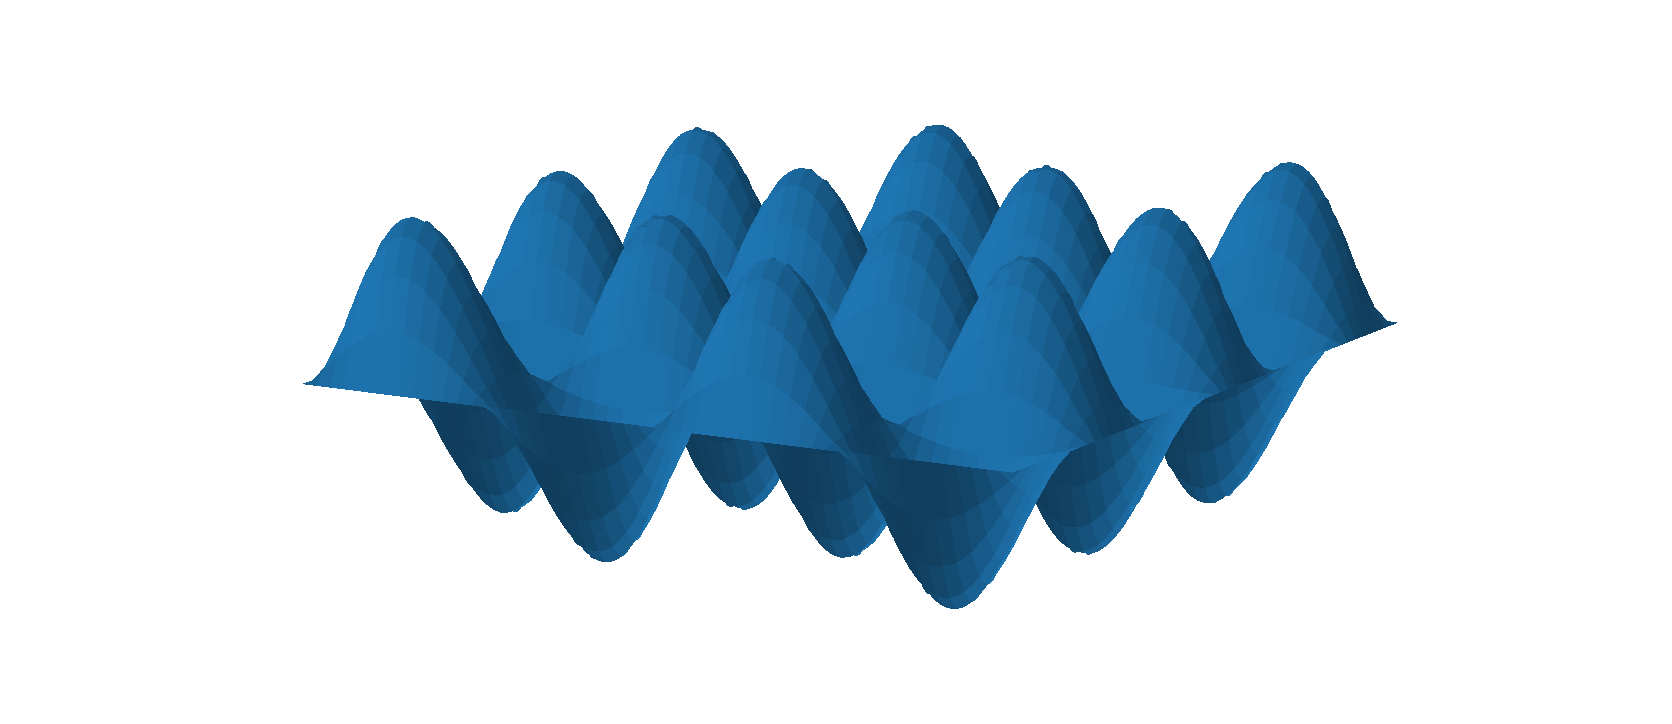
\includegraphics[width=.8\textwidth]{images/optlat/default.pdf}
  \captionsetup{width=.8\textwidth}
  \caption{Periodic potential of a 2D optical lattice. If the kinetic energy
  of the atoms is below the potential energy of the lattice, the atoms will
  locate around the potential minimas.}
  \label{fig:optlat}
\end{figure}

One of the parameters of interest is the ability to apply local potentials
to the system, that can be used to, among others, study lattice inpurities
or quantum interactions. In this work we will present and characterize one
possible implementation of such a local potential generating apparatus.

\section{Related Work}

Local manipulations of atoms inside optical lattices have been known for some
time in the embodiment of optical tweezers that allow trapping, stacking and
sorting of particles \cite{Tadmor2004}. Yet, only recently attempts to
interact with local particle clusters through high-precision time-averaged
optical potentials have been reported \cite{Roy2016}.

In the following we continue on the laid out work \cite{Hertlein2017} which
provided us with an optical setup for single-site manipulation using
\gls{aod} as well as considerations with regard to aperture limited
gaussian beam propagation.

\chapter{Optical potentials}

\textit{In the introduction we emphasized the importance of optical lattices,
yet we left out many details, for instance, how these optical lattices are
created and how the optical quantities enter the potential energy of the
atoms. In this chapter we will make up for said gaps. First we will
recapitulate the theory behind laser light intensities and then derive a
formulation of the effective lattice potentials felt by the atoms.}

\section{Atom-light interaction}

At first we need to ask ourselves how the laser field acts as a perturbation
to the Hamiltonian of the atomic system and how this perturbation leads to an
intensity dependent potential for the atoms, which we can control in the
experiment. In deviations are loosely based on
references~\cite{Gerry2004,Jackson2005,Bartelmann2018}.

\subsection{Dipole potential}

We will use \gls{si} units unless stated otherwise. The Hamiltonian of an electron
in an external electromagnetic field reads
\begin{equation}
  \hat{H}_\text{em}
  =\frac{1}{2m_e}{\left(\hat{\vb{p}}+e\vb{A}\right)}^2-e\Phi+\hat{V}_0
  \label{eq:hamiltonian_em},
\end{equation}
with vector potential $\vb{A}$ and scalar potential $\Phi$ of the external
field and the Coulomb potential of the nucleus $\hat{V}_0$. Further $m_e$
denotes the electron mass and $e$ the elementary charge.
\Cref{eq:hamiltonian_em} is exact for the hydrogen atom that only hosts one
electron. For alkali atoms we know that inner electron shells are closed and
the single outer electron is approximately described by
\cref{eq:hamiltonian_em}. The electromagnetic field relates to the
vector and scalar potential through
\begin{align}
  \vb{E}=-\grad{\Phi}-\pdv{\vb{A}}{t}, &&
  \vb{B}=\curl{\vb{A}},
  \label{eq:field_em_potentials}
\end{align}
where $\vb{E}$ is the electric and $\vb{B}$ the magnetic field component.

The canonical momentum $\hat{\vb{p}}+e\vb{A}$ in \cref{eq:hamiltonian_em} is
difficult to work with. Fortunately Gauge transforms
\begin{align}
  \vb{A}\to\vb{A}+\grad{\chi}
  &&
  \Phi\to\Phi-\pdv{\chi}{t}
  \label{eq:gauge_transform_em}
\end{align}
allow us to simplify \cref{eq:hamiltonian_em} by choosing a specific Gauge
function $\chi(\vb{x},t)$. The Gauge function itself $\chi$ does not amend the
electromagnetic field components \cref{eq:field_em_potentials} which we
usually consider to represent physical reality --- in contrast to the
electromagnetic potentials $\vb{A},\Phi$ which are usually only considered
mathematical aid.\footnote{The Aharonov-Bohm effect actually provides evidence
that aso the electromagnetic potentials represent physical reality.} In the
following we choose the gauge function $\chi=-\vb{A}\cdot\vb{x}$ and assume
the dipole approximation $\vb{A}(\vb{x},t)\approx\vb{A}(t)$. The dipole
approximation neglects the spatial variation of the electromagnetic field
over the atom and instead assumes a small separation of opposite charges at
the nucleus. The dipole approximation is reasonable as wave length of visible
light are much larger than atomic length scales~\cite{Gerry2004}. For a
rigorous upper error bound on the dipole approximation see
Ref.~\cite{Bossmann2016}. In the dipole approximation $\chi$ satisfies the
Coulomb gauge condition $\divergence{\vb{A}}=0$ allowing us to set $\Phi=0$
as no external sources are present~\cite{Jackson2005}. Finally we can rewrite
\cref{eq:hamiltonian_em} as
\begin{equation}
  \hat{H}_\text{dip}
  =\frac{\hat{\vb{p}}^2}{2m}+\hat{V}_0+\hat{V}_\text{dip}
  =\hat{H}_0+\hat{V}_\text{dip}
  \label{eq:hamiltonian_dip}
\end{equation}
with the dipole potential
\begin{equation}
  \hat{V}_\text{dip}
  =-\hat{\vb{d}}\cdot\vb{E}
  \label{eq:potential_dip},
\end{equation}
the dipole operator $\hat{\vb{d}}=-e\vb{x}$ and the spatially homogeneous
light field $\vb{E}(t)$.

\subsection{AC-Stark effect}

We are now going to solve \cref{eq:hamiltonian_dip} for an arbitrary light
field of the form
\begin{equation}
  \vb{E}(t,\vb{x})
  =\vb{E}_0(\vb{x})\cos(\omega t)
  \label{eq:light_field}
\end{equation}
where $\vb{E}_0(\vb{x})$ should be compatible with Maxwell's equations and
be approximately constant on atomic length scales to not violate the dipole
approximation. Further we need the laser frequency $\omega$ to be
far-off-resonant to the atomic transition frequencies to avoid population
dynamics.

At $t<0$ the system is in the energy eigenstate $\ket{n}$ of the
unperturbated Hamiltonian $\hat{H}_0$
\begin{equation}
  \hat{H}_0\ket{n}
  =E_n\ket{n}
  =\hbar\omega_n\ket{n}
  \label{eq:eigenvalue_energy_unperturbated}.
\end{equation}
At $t>0$ the external light field appears immediately. The new state
$\ket{\psi}$ can be expanded in the complete basis of the previous energy
eigenstates
\begin{equation}
  \ket{\psi}
  =
  \sum_n{c_n(t)}{e^{-i{\omega_n}t}}\ket{n}
  \label{eq:state_expansion_unperturbated}.
\end{equation}
Inserting \cref{eq:state_expansion_unperturbated} into the time-dependent
Schrödinger equation with the dipole Hamiltonian \cref{eq:hamiltonian_dip} and
applying $\bra{m}{e^{i{\omega_m}t}}$ to the right hand side leads us to a set
of differential equations
\begin{equation}
  \dot{c}_m
  =
  -\frac{i}{\hbar}\sum_n{c_n(t)}{e^{-i\omega_{nm}t}}
  \bra{m}\hat{V}_\text{dip}\ket{n}
  \label{eq:differential_equation_population_dynamics}
\end{equation}
with $\omega_{nm}=\omega_n-\omega_m$. One can read
\cref{eq:differential_equation_population_dynamics} as the rate by which
the probability amplitude of a state $m$ changes in time. It is equal to the
sum of oscillations between states $n$ and $m$ weighted by the current
probability of state $c_n(t)$ and the interaction strength. If we are able to
solve \cref{eq:differential_equation_population_dynamics} for $c_n(t)$ the
population dynamic is entirely described by the time-dependent probabilities
$\abs{c_n(t)}^2$. By using \cref{eq:light_field} we can rewrite the dipole
transition matrix elements
\begin{equation}
  \bra{m}\hat{V}_\text{dip}\ket{n}
  =\Omega_{nm}(\vb{x})\cos(\omega t)\hbar
  \label{eq:elements_dipole_transition_matrix}
\end{equation}
where we introduced the Rabi frequency
\begin{equation}
  \Omega_{nm}(\vb{x})
  =\bra{n}\hat{\vb{d}}\cdot\vb{E}_0(\vb{x})\ket{m}/\hbar
  \label{eq:rabi_frequency}.
\end{equation}
More general expressions for dipole transition elements of one and two
electron systems can be found in Reference~\cite{Bethe1957}. 

\subsubsection{Two-level system}

From now on we assume a two state system that initially is in the ground
state $c_g(0)=1,c_e(0)=0$. Under these circumstances the dynamics described in
\cref{eq:differential_equation_population_dynamics} simplify to
\begin{align}
  i\dot{c}_g=\Omega_{ge}c_e(t)\cos(\omega t)e^{+i\omega_0 t} &&
  i\dot{c}_e=\Omega_{ge}c_g(t)\cos(\omega t)e^{-i\omega_0 t}
  \label{eq:differential_equation_population_dynamics_two_state_system}
\end{align}
Writing $\cos(\omega t)$ in terms of exponential functions and dropping
$e^{\pm i(\omega+\omega_{ge})t}$ yields the so-called \gls{rwa}
\begin{align}
  i\dot{c}_g\approx\frac{\Omega_{ge}}{2}c_e(t)e^{+i\Delta\omega t} &&
  i\dot{c}_e\approx\frac{\Omega_{ge}}{2}c_g(t)e^{-i\Delta\omega t}
  \label{eq:differential_equation_population_dynamics_two_state_system_rwa}
\end{align}
where we introduced the frequency detuning
$\Delta\omega=\abs{\omega-\omega_0}$. The \gls{rwa} is motivated by the fact
that oscillations of frequency $\omega+\omega_0$ are fast compared to changes
in the population dynamics and therefore vanish on average.

We now define $a_g=c_g$ and $a_e=c_e e^{i\Delta\omega t}$ and rewrite
\cref{eq:differential_equation_population_dynamics_two_state_system_rwa} by
\begin{align}
  i\dot{a}_g=\frac{\Omega_{ge}}{2}a_e(t) &&
  i\dot{a}_e=\frac{\Omega_{ge}}{2}a_g(t)-a_e\Delta\omega
  \label{eq:differential_equation_population_dynamics_two_state_system_shift}.
\end{align}
Using
\cref{eq:differential_equation_population_dynamics_two_state_system_shift} we
can diagonalize the Hamiltonian and find the energy eigenvalues to be
\begin{equation}
  E_{e,g}
  =\frac{\hbar}{2}\left(-\Delta\omega\mp\sqrt{\Omega_{ge}^2+\Delta\omega^2}\right)
  \approx
  \mp\frac{\hbar\Omega_{ge}^2}{4\Delta\omega}
  \label{eq:eigenvalues_energy_light_shift}
\end{equation}
where we applied a Taylor expansion for $\Omega_{ge}/\Delta\omega\ll1$ around
$\Omega_{ge}/\Delta\omega=0$ and omitted terms of higher order.

Consequently, atoms in an external off-resonant light field experience an
effective periodic lattice potential
\begin{equation}
  \hat{V}_\text{lat}(\vb{x})
  =
  \mp\frac{\hbar\Omega_{ge}^2(\vb{x})}{4\Delta\omega}
  =
  \mp\frac{d_0^2E_0^2(\vb{x})}{4\hbar\Delta\omega}
  \label{eq:potential_lattice}
\end{equation}
with dipole element $d_0$. The sign has to be chosen with respect to the
direction of the laser detuning from resonance. If the laser is red-shifted
compared to the resonance frequency, $\omega-\omega_0>0$, we need to choose
the negative sign as the particles are drawn towards the areas of maximum
intensity. If the laser is blue-shifted compared to the resonance frequency,
$\omega-\omega_0<0$, we need to choose the positive sign as the particles are
drawn towards the area of minimum intensity. The same results can also be
obtained by the use of second order perturbation theory~\cite{Grimm2008}.

\section{Laser light fields}

In this section our focus will be on the spatial distribution of the lattice
and perturbation laser light fields that create the time-averaged dynamical
potentials we discussed in the introduction.

\subsection{Gaussian beams}

The predominant output mode of most lasers is the fundamental transverse
gaussian mode. For a laser beam propagating along the $z$-direction it is
described by
\begin{equation}
  \vb{E}(r,z)
  =
  \vb{E}_0\frac{w(0)}{w(z)}
  \exp{-\frac{r^2}{w{(z)}^2}}
  \exp{-ik\left(z+\frac{r^2}{2R(z)}-\arctan(\frac{z}{z_R})\right)}
  \label{eq:gaussian_beam}
\end{equation}
where $w{(z)}$ is the waist radius, $z_R=\pi w{(0)}^2/\lambda$ the Rayleigh
range and $R(z)$ the radius of curvature of the beam's wavefront at position
$z$.
\begin{figure}[ht]
  \centering
  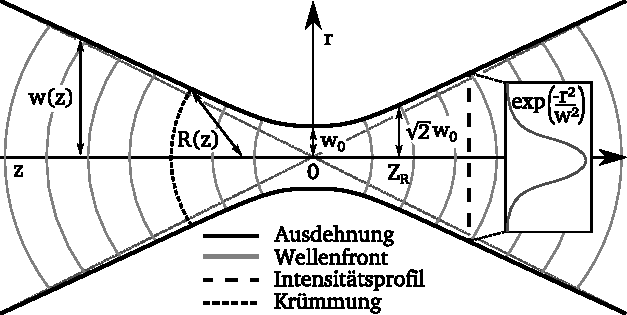
\includegraphics[width=.9\textwidth]{\mediadir{image/gaussian-beam.pdf}}
  \captionsetup{width=.9\textwidth}
  \caption{Illustration of Gaussian beam parameters from Ref.~\cite{Aleph2014}
    translated into English with changed radius of curvature.
  }\label{fig:gaussian_beam}
\end{figure}
\Cref{fig:gaussian_beam} unveils how the parameters relate to the beam
profile as a function of propagation distance $z$. The waist radius $w(z)$
corresponds to the \gls{fwhm} by $w(z)=FWHM(z)/\sqrt{2\ln2}$, $R(z)$ relates
to the wavefront curvature and $z_R$ is the distance from origin $z=0$ where
the beam waist is $w(z)=\sqrt{2}w(0)$. Beam waist and curvature of radius
evolve according to
\begin{align}
  w{(z)}
  =
  w{(0)}{\left[1+{\left(\frac{z}{z_R}\right)}^2\right]}^{1/2}
  &&
  R{(z)}=z{\left[1+{\left(\frac{z_R}{z}\right)}^2\right]}
  \label{eq:gaussian_beam_evolvement}.
\end{align}

Fortunately \cref{eq:potential_lattice} only depends on the absolute
square of the electric field, thus we can drop the complex exponential from
\cref{eq:gaussian_beam} to find an expression for the Gaussian intensity
distribution
\begin{equation}
  I(r,z)
  =
  I_0
  {\left(\frac{w(0)}{w(z)}\right)}^2
  \exp{-\frac{2r^2}{w{(z)}^2}}
  =
  I_0
  \frac{\exp{-\frac{2r^2}{w{(z)}^2}}}{1+{\left(\frac{z}{z_R}\right)}^2}
  \label{eq:gaussian_intensity}
\end{equation}
where $I_0$ is the maximum intensity at $r=z=0$.

\subsubsection{Lattice intensity}

A \gls{1d} optical lattices can be generated through the interference
of two counter-propagating Gaussian beams. One way to achieve
counter-propagation while keeping the coherence stable, is to use a mirror.
Under the assumption of perfect reflection of the mirror, the electrical field
component of the laser beam is described by
\begin{align*}
  \vb{E}_\rightarrow(\vb{x},t)+\vb{E}_\leftarrow(\vb{x},t)
  &=
  \vb{E}_0(r,z)\cos(\omega t-kz)+\vb{E}_0(r,z)\cos(\omega t+kz)\\
  &=
  2\vb{E}_0(r,z)\cos(kz)\cos(\omega t).
\end{align*}
Hence, the intensity distribution equals
\cref{eq:gaussian_intensity} with an additional $4\cos^2(kz)$ factor
\begin{equation}
  I(r,z)
  =
  4I_0\cos^2(kz)
  \frac{\exp{-\frac{2r^2}{w{(z)}^2}}}{1+{\left(\frac{z}{z_R}\right)}^2}
  \label{eq:lattice_intensity}
\end{equation}
caused by the constructive interference.
\begin{table}[ht]
  \centering
  \begin{tabular}{cccc}
    \toprule
    Laser wavelength $\lambda$ &
    Lattice constant $a=\lambda/2$ &
    Beam waist $w(0)$ &
    Rayleigh length $z_R$ \\
    \midrule
    \SI{1064}{\nano\meter} &
    \SI{532}{\nano\meter} &
    \SI{150}{\micro\meter} &
    \SI{66}{\milli\meter} \\
    \bottomrule
  \end{tabular}
  \captionsetup{width=.8\textwidth}
  \caption{Typical values for a Gaussian beam used to generate an optical
    lattice potential.
  }\label{tab:gaussian_beam_lattice}
\end{table}
\Cref{tab:gaussian_beam_lattice} lists typical values for a Gaussian beam
used to construct an optical lattice potential. Typical atom clouds occupy
about 50--100 lattice sites spanning over a range of
$l=50a\approx\SI{27}{\micro\meter}$~\cite{Rom2009}. As typical atom clouds
are much smaller then the typical beam waists used for optical lattices, we
have $r/w(z)\ll1$ and can approximate \cref{eq:lattice_intensity}
\begin{equation}
  I(r,z)
  \approx
  4I_0\cos^2(kz)
  \label{eq:gaussian_intensity_approx}
\end{equation}
which we will use from now on as the intensity distribution for \gls{1d}
optical lattices.

\subsubsection{Perturbation intensity}

For the generation of optical lattices we want large beam waists because
otherwise the potential is not homogeneous and there is a potential energy
difference between neighboring lattice sites. For our perturbation potential,
however, we need very high resolution on the order of a single lattice site,
and therefore need a tightly focused beam.
\begin{table}[ht]
  \centering
  \begin{tabular}{cccc}
    \toprule
    Laser wavelength $\lambda$ &
    Beam waist $w(0)$ &
    Rayleigh length $z_R$ \\
    \midrule
    \SI{532}{\nano\meter} &
    \SI{1}{\micro\meter} &
    \SI{6}{\micro\meter} \\
    \bottomrule
  \end{tabular}
  \captionsetup{width=.8\textwidth}
  \caption{Typical values for a Gaussian beam used to perturbate the optical
    lattice potential reported by~\cite{Hertlein2017}.
  }\label{tab:gaussian_beam_perturbation}
\end{table}
\Cref{tab:gaussian_beam_perturbation} summarizes the beam parameter of the
perturbation potential as suggested in Ref.~\cite{Hertlein2017}. For these
parameters approximations made for optical lattice are not valid because of
the small beam waist and Rayleigh length and we need to the exact
\cref{eq:gaussian_intensity} formula. In fact for an actual experiment we
would like to focus the laser beam to even smaller waists. The ultimate goal
would be the ability to address single lattice sites.

\section{Effective local potentials}

With \cref{eq:potential_lattice} we found an expression of the potential
energy in terms of atomic properties like the dipole transition element, the
atomic resonance and the laser intensity distribution. For the laser intensity
distribution of the optical lattice we derived
\cref{eq:gaussian_intensity_approx} and we concluded that the intensity of the
laser used for the creation of local potentials obeys
\cref{eq:gaussian_intensity}. If we add these pieces together we can calculate
the effective potential with local perturbation as seen by the atoms. We will
find that its shape deviates from the idealized local potentials we presented
in the introduction in \Cref{fig:optical_lattice_local_pot} and 
\Cref{fig:optical_lattice_local_barrier}.

\subsubsection{Barrier}

One embodiment of local potentials we described in the introduction was the
barrier potential. A barrier potential confines atoms to a subspace of the
global lattice and could be used to model thermodynamical equilibrium
processes.
\begin{figure}[htb]
  \centering
  \begin{adjustbox}{width=\textwidth}
    %% Creator: Matplotlib, PGF backend
%%
%% To include the figure in your LaTeX document, write
%%   \input{<filename>.pgf}
%%
%% Make sure the required packages are loaded in your preamble
%%   \usepackage{pgf}
%%
%% Figures using additional raster images can only be included by \input if
%% they are in the same directory as the main LaTeX file. For loading figures
%% from other directories you can use the `import` package
%%   \usepackage{import}
%% and then include the figures with
%%   \import{<path to file>}{<filename>.pgf}
%%
%% Matplotlib used the following preamble
%%   \usepackage{amsmath}\usepackage{siunitx}\usepackage{lmodern}
%%   \usepackage{fontspec}
%%
\begingroup%
\makeatletter%
\begin{pgfpicture}%
\pgfpathrectangle{\pgfpointorigin}{\pgfqpoint{12.000000in}{8.000000in}}%
\pgfusepath{use as bounding box, clip}%
\begin{pgfscope}%
\pgfsetbuttcap%
\pgfsetmiterjoin%
\pgfsetlinewidth{0.000000pt}%
\definecolor{currentstroke}{rgb}{1.000000,1.000000,1.000000}%
\pgfsetstrokecolor{currentstroke}%
\pgfsetdash{}{0pt}%
\pgfpathmoveto{\pgfqpoint{0.000000in}{0.000000in}}%
\pgfpathlineto{\pgfqpoint{12.000000in}{0.000000in}}%
\pgfpathlineto{\pgfqpoint{12.000000in}{8.000000in}}%
\pgfpathlineto{\pgfqpoint{0.000000in}{8.000000in}}%
\pgfpathclose%
\pgfusepath{}%
\end{pgfscope}%
\begin{pgfscope}%
\pgfsetbuttcap%
\pgfsetmiterjoin%
\definecolor{currentfill}{rgb}{1.000000,1.000000,1.000000}%
\pgfsetfillcolor{currentfill}%
\pgfsetlinewidth{0.000000pt}%
\definecolor{currentstroke}{rgb}{0.000000,0.000000,0.000000}%
\pgfsetstrokecolor{currentstroke}%
\pgfsetstrokeopacity{0.000000}%
\pgfsetdash{}{0pt}%
\pgfpathmoveto{\pgfqpoint{1.500000in}{5.740000in}}%
\pgfpathlineto{\pgfqpoint{10.800000in}{5.740000in}}%
\pgfpathlineto{\pgfqpoint{10.800000in}{7.840000in}}%
\pgfpathlineto{\pgfqpoint{1.500000in}{7.840000in}}%
\pgfpathclose%
\pgfusepath{fill}%
\end{pgfscope}%
\begin{pgfscope}%
\pgfsetbuttcap%
\pgfsetroundjoin%
\definecolor{currentfill}{rgb}{0.000000,0.000000,0.000000}%
\pgfsetfillcolor{currentfill}%
\pgfsetlinewidth{1.003750pt}%
\definecolor{currentstroke}{rgb}{0.000000,0.000000,0.000000}%
\pgfsetstrokecolor{currentstroke}%
\pgfsetdash{}{0pt}%
\pgfsys@defobject{currentmarker}{\pgfqpoint{0.000000in}{0.000000in}}{\pgfqpoint{0.000000in}{0.055556in}}{%
\pgfpathmoveto{\pgfqpoint{0.000000in}{0.000000in}}%
\pgfpathlineto{\pgfqpoint{0.000000in}{0.055556in}}%
\pgfusepath{stroke,fill}%
}%
\begin{pgfscope}%
\pgfsys@transformshift{3.003069in}{5.740000in}%
\pgfsys@useobject{currentmarker}{}%
\end{pgfscope}%
\end{pgfscope}%
\begin{pgfscope}%
\pgfsetbuttcap%
\pgfsetroundjoin%
\definecolor{currentfill}{rgb}{0.000000,0.000000,0.000000}%
\pgfsetfillcolor{currentfill}%
\pgfsetlinewidth{1.003750pt}%
\definecolor{currentstroke}{rgb}{0.000000,0.000000,0.000000}%
\pgfsetstrokecolor{currentstroke}%
\pgfsetdash{}{0pt}%
\pgfsys@defobject{currentmarker}{\pgfqpoint{0.000000in}{-0.055556in}}{\pgfqpoint{0.000000in}{0.000000in}}{%
\pgfpathmoveto{\pgfqpoint{0.000000in}{0.000000in}}%
\pgfpathlineto{\pgfqpoint{0.000000in}{-0.055556in}}%
\pgfusepath{stroke,fill}%
}%
\begin{pgfscope}%
\pgfsys@transformshift{3.003069in}{7.840000in}%
\pgfsys@useobject{currentmarker}{}%
\end{pgfscope}%
\end{pgfscope}%
\begin{pgfscope}%
\pgfsetbuttcap%
\pgfsetroundjoin%
\definecolor{currentfill}{rgb}{0.000000,0.000000,0.000000}%
\pgfsetfillcolor{currentfill}%
\pgfsetlinewidth{1.003750pt}%
\definecolor{currentstroke}{rgb}{0.000000,0.000000,0.000000}%
\pgfsetstrokecolor{currentstroke}%
\pgfsetdash{}{0pt}%
\pgfsys@defobject{currentmarker}{\pgfqpoint{0.000000in}{0.000000in}}{\pgfqpoint{0.000000in}{0.055556in}}{%
\pgfpathmoveto{\pgfqpoint{0.000000in}{0.000000in}}%
\pgfpathlineto{\pgfqpoint{0.000000in}{0.055556in}}%
\pgfusepath{stroke,fill}%
}%
\begin{pgfscope}%
\pgfsys@transformshift{4.576534in}{5.740000in}%
\pgfsys@useobject{currentmarker}{}%
\end{pgfscope}%
\end{pgfscope}%
\begin{pgfscope}%
\pgfsetbuttcap%
\pgfsetroundjoin%
\definecolor{currentfill}{rgb}{0.000000,0.000000,0.000000}%
\pgfsetfillcolor{currentfill}%
\pgfsetlinewidth{1.003750pt}%
\definecolor{currentstroke}{rgb}{0.000000,0.000000,0.000000}%
\pgfsetstrokecolor{currentstroke}%
\pgfsetdash{}{0pt}%
\pgfsys@defobject{currentmarker}{\pgfqpoint{0.000000in}{-0.055556in}}{\pgfqpoint{0.000000in}{0.000000in}}{%
\pgfpathmoveto{\pgfqpoint{0.000000in}{0.000000in}}%
\pgfpathlineto{\pgfqpoint{0.000000in}{-0.055556in}}%
\pgfusepath{stroke,fill}%
}%
\begin{pgfscope}%
\pgfsys@transformshift{4.576534in}{7.840000in}%
\pgfsys@useobject{currentmarker}{}%
\end{pgfscope}%
\end{pgfscope}%
\begin{pgfscope}%
\pgfsetbuttcap%
\pgfsetroundjoin%
\definecolor{currentfill}{rgb}{0.000000,0.000000,0.000000}%
\pgfsetfillcolor{currentfill}%
\pgfsetlinewidth{1.003750pt}%
\definecolor{currentstroke}{rgb}{0.000000,0.000000,0.000000}%
\pgfsetstrokecolor{currentstroke}%
\pgfsetdash{}{0pt}%
\pgfsys@defobject{currentmarker}{\pgfqpoint{0.000000in}{0.000000in}}{\pgfqpoint{0.000000in}{0.055556in}}{%
\pgfpathmoveto{\pgfqpoint{0.000000in}{0.000000in}}%
\pgfpathlineto{\pgfqpoint{0.000000in}{0.055556in}}%
\pgfusepath{stroke,fill}%
}%
\begin{pgfscope}%
\pgfsys@transformshift{6.150000in}{5.740000in}%
\pgfsys@useobject{currentmarker}{}%
\end{pgfscope}%
\end{pgfscope}%
\begin{pgfscope}%
\pgfsetbuttcap%
\pgfsetroundjoin%
\definecolor{currentfill}{rgb}{0.000000,0.000000,0.000000}%
\pgfsetfillcolor{currentfill}%
\pgfsetlinewidth{1.003750pt}%
\definecolor{currentstroke}{rgb}{0.000000,0.000000,0.000000}%
\pgfsetstrokecolor{currentstroke}%
\pgfsetdash{}{0pt}%
\pgfsys@defobject{currentmarker}{\pgfqpoint{0.000000in}{-0.055556in}}{\pgfqpoint{0.000000in}{0.000000in}}{%
\pgfpathmoveto{\pgfqpoint{0.000000in}{0.000000in}}%
\pgfpathlineto{\pgfqpoint{0.000000in}{-0.055556in}}%
\pgfusepath{stroke,fill}%
}%
\begin{pgfscope}%
\pgfsys@transformshift{6.150000in}{7.840000in}%
\pgfsys@useobject{currentmarker}{}%
\end{pgfscope}%
\end{pgfscope}%
\begin{pgfscope}%
\pgfsetbuttcap%
\pgfsetroundjoin%
\definecolor{currentfill}{rgb}{0.000000,0.000000,0.000000}%
\pgfsetfillcolor{currentfill}%
\pgfsetlinewidth{1.003750pt}%
\definecolor{currentstroke}{rgb}{0.000000,0.000000,0.000000}%
\pgfsetstrokecolor{currentstroke}%
\pgfsetdash{}{0pt}%
\pgfsys@defobject{currentmarker}{\pgfqpoint{0.000000in}{0.000000in}}{\pgfqpoint{0.000000in}{0.055556in}}{%
\pgfpathmoveto{\pgfqpoint{0.000000in}{0.000000in}}%
\pgfpathlineto{\pgfqpoint{0.000000in}{0.055556in}}%
\pgfusepath{stroke,fill}%
}%
\begin{pgfscope}%
\pgfsys@transformshift{7.723466in}{5.740000in}%
\pgfsys@useobject{currentmarker}{}%
\end{pgfscope}%
\end{pgfscope}%
\begin{pgfscope}%
\pgfsetbuttcap%
\pgfsetroundjoin%
\definecolor{currentfill}{rgb}{0.000000,0.000000,0.000000}%
\pgfsetfillcolor{currentfill}%
\pgfsetlinewidth{1.003750pt}%
\definecolor{currentstroke}{rgb}{0.000000,0.000000,0.000000}%
\pgfsetstrokecolor{currentstroke}%
\pgfsetdash{}{0pt}%
\pgfsys@defobject{currentmarker}{\pgfqpoint{0.000000in}{-0.055556in}}{\pgfqpoint{0.000000in}{0.000000in}}{%
\pgfpathmoveto{\pgfqpoint{0.000000in}{0.000000in}}%
\pgfpathlineto{\pgfqpoint{0.000000in}{-0.055556in}}%
\pgfusepath{stroke,fill}%
}%
\begin{pgfscope}%
\pgfsys@transformshift{7.723466in}{7.840000in}%
\pgfsys@useobject{currentmarker}{}%
\end{pgfscope}%
\end{pgfscope}%
\begin{pgfscope}%
\pgfsetbuttcap%
\pgfsetroundjoin%
\definecolor{currentfill}{rgb}{0.000000,0.000000,0.000000}%
\pgfsetfillcolor{currentfill}%
\pgfsetlinewidth{1.003750pt}%
\definecolor{currentstroke}{rgb}{0.000000,0.000000,0.000000}%
\pgfsetstrokecolor{currentstroke}%
\pgfsetdash{}{0pt}%
\pgfsys@defobject{currentmarker}{\pgfqpoint{0.000000in}{0.000000in}}{\pgfqpoint{0.000000in}{0.055556in}}{%
\pgfpathmoveto{\pgfqpoint{0.000000in}{0.000000in}}%
\pgfpathlineto{\pgfqpoint{0.000000in}{0.055556in}}%
\pgfusepath{stroke,fill}%
}%
\begin{pgfscope}%
\pgfsys@transformshift{9.296931in}{5.740000in}%
\pgfsys@useobject{currentmarker}{}%
\end{pgfscope}%
\end{pgfscope}%
\begin{pgfscope}%
\pgfsetbuttcap%
\pgfsetroundjoin%
\definecolor{currentfill}{rgb}{0.000000,0.000000,0.000000}%
\pgfsetfillcolor{currentfill}%
\pgfsetlinewidth{1.003750pt}%
\definecolor{currentstroke}{rgb}{0.000000,0.000000,0.000000}%
\pgfsetstrokecolor{currentstroke}%
\pgfsetdash{}{0pt}%
\pgfsys@defobject{currentmarker}{\pgfqpoint{0.000000in}{-0.055556in}}{\pgfqpoint{0.000000in}{0.000000in}}{%
\pgfpathmoveto{\pgfqpoint{0.000000in}{0.000000in}}%
\pgfpathlineto{\pgfqpoint{0.000000in}{-0.055556in}}%
\pgfusepath{stroke,fill}%
}%
\begin{pgfscope}%
\pgfsys@transformshift{9.296931in}{7.840000in}%
\pgfsys@useobject{currentmarker}{}%
\end{pgfscope}%
\end{pgfscope}%
\begin{pgfscope}%
\pgfsetbuttcap%
\pgfsetroundjoin%
\definecolor{currentfill}{rgb}{0.000000,0.000000,0.000000}%
\pgfsetfillcolor{currentfill}%
\pgfsetlinewidth{1.003750pt}%
\definecolor{currentstroke}{rgb}{0.000000,0.000000,0.000000}%
\pgfsetstrokecolor{currentstroke}%
\pgfsetdash{}{0pt}%
\pgfsys@defobject{currentmarker}{\pgfqpoint{0.000000in}{0.000000in}}{\pgfqpoint{0.055556in}{0.000000in}}{%
\pgfpathmoveto{\pgfqpoint{0.000000in}{0.000000in}}%
\pgfpathlineto{\pgfqpoint{0.055556in}{0.000000in}}%
\pgfusepath{stroke,fill}%
}%
\begin{pgfscope}%
\pgfsys@transformshift{1.500000in}{5.835454in}%
\pgfsys@useobject{currentmarker}{}%
\end{pgfscope}%
\end{pgfscope}%
\begin{pgfscope}%
\pgfsetbuttcap%
\pgfsetroundjoin%
\definecolor{currentfill}{rgb}{0.000000,0.000000,0.000000}%
\pgfsetfillcolor{currentfill}%
\pgfsetlinewidth{1.003750pt}%
\definecolor{currentstroke}{rgb}{0.000000,0.000000,0.000000}%
\pgfsetstrokecolor{currentstroke}%
\pgfsetdash{}{0pt}%
\pgfsys@defobject{currentmarker}{\pgfqpoint{-0.055556in}{0.000000in}}{\pgfqpoint{0.000000in}{0.000000in}}{%
\pgfpathmoveto{\pgfqpoint{0.000000in}{0.000000in}}%
\pgfpathlineto{\pgfqpoint{-0.055556in}{0.000000in}}%
\pgfusepath{stroke,fill}%
}%
\begin{pgfscope}%
\pgfsys@transformshift{10.800000in}{5.835454in}%
\pgfsys@useobject{currentmarker}{}%
\end{pgfscope}%
\end{pgfscope}%
\begin{pgfscope}%
\pgftext[x=1.155864in,y=5.787260in,left,base]{\fontsize{10.000000}{12.000000}\selectfont \(\displaystyle -10\)}%
\end{pgfscope}%
\begin{pgfscope}%
\pgfsetbuttcap%
\pgfsetroundjoin%
\definecolor{currentfill}{rgb}{0.000000,0.000000,0.000000}%
\pgfsetfillcolor{currentfill}%
\pgfsetlinewidth{1.003750pt}%
\definecolor{currentstroke}{rgb}{0.000000,0.000000,0.000000}%
\pgfsetstrokecolor{currentstroke}%
\pgfsetdash{}{0pt}%
\pgfsys@defobject{currentmarker}{\pgfqpoint{0.000000in}{0.000000in}}{\pgfqpoint{0.055556in}{0.000000in}}{%
\pgfpathmoveto{\pgfqpoint{0.000000in}{0.000000in}}%
\pgfpathlineto{\pgfqpoint{0.055556in}{0.000000in}}%
\pgfusepath{stroke,fill}%
}%
\begin{pgfscope}%
\pgfsys@transformshift{1.500000in}{6.312788in}%
\pgfsys@useobject{currentmarker}{}%
\end{pgfscope}%
\end{pgfscope}%
\begin{pgfscope}%
\pgfsetbuttcap%
\pgfsetroundjoin%
\definecolor{currentfill}{rgb}{0.000000,0.000000,0.000000}%
\pgfsetfillcolor{currentfill}%
\pgfsetlinewidth{1.003750pt}%
\definecolor{currentstroke}{rgb}{0.000000,0.000000,0.000000}%
\pgfsetstrokecolor{currentstroke}%
\pgfsetdash{}{0pt}%
\pgfsys@defobject{currentmarker}{\pgfqpoint{-0.055556in}{0.000000in}}{\pgfqpoint{0.000000in}{0.000000in}}{%
\pgfpathmoveto{\pgfqpoint{0.000000in}{0.000000in}}%
\pgfpathlineto{\pgfqpoint{-0.055556in}{0.000000in}}%
\pgfusepath{stroke,fill}%
}%
\begin{pgfscope}%
\pgfsys@transformshift{10.800000in}{6.312788in}%
\pgfsys@useobject{currentmarker}{}%
\end{pgfscope}%
\end{pgfscope}%
\begin{pgfscope}%
\pgftext[x=1.225308in,y=6.264593in,left,base]{\fontsize{10.000000}{12.000000}\selectfont \(\displaystyle -5\)}%
\end{pgfscope}%
\begin{pgfscope}%
\pgfsetbuttcap%
\pgfsetroundjoin%
\definecolor{currentfill}{rgb}{0.000000,0.000000,0.000000}%
\pgfsetfillcolor{currentfill}%
\pgfsetlinewidth{1.003750pt}%
\definecolor{currentstroke}{rgb}{0.000000,0.000000,0.000000}%
\pgfsetstrokecolor{currentstroke}%
\pgfsetdash{}{0pt}%
\pgfsys@defobject{currentmarker}{\pgfqpoint{0.000000in}{0.000000in}}{\pgfqpoint{0.055556in}{0.000000in}}{%
\pgfpathmoveto{\pgfqpoint{0.000000in}{0.000000in}}%
\pgfpathlineto{\pgfqpoint{0.055556in}{0.000000in}}%
\pgfusepath{stroke,fill}%
}%
\begin{pgfscope}%
\pgfsys@transformshift{1.500000in}{6.790122in}%
\pgfsys@useobject{currentmarker}{}%
\end{pgfscope}%
\end{pgfscope}%
\begin{pgfscope}%
\pgfsetbuttcap%
\pgfsetroundjoin%
\definecolor{currentfill}{rgb}{0.000000,0.000000,0.000000}%
\pgfsetfillcolor{currentfill}%
\pgfsetlinewidth{1.003750pt}%
\definecolor{currentstroke}{rgb}{0.000000,0.000000,0.000000}%
\pgfsetstrokecolor{currentstroke}%
\pgfsetdash{}{0pt}%
\pgfsys@defobject{currentmarker}{\pgfqpoint{-0.055556in}{0.000000in}}{\pgfqpoint{0.000000in}{0.000000in}}{%
\pgfpathmoveto{\pgfqpoint{0.000000in}{0.000000in}}%
\pgfpathlineto{\pgfqpoint{-0.055556in}{0.000000in}}%
\pgfusepath{stroke,fill}%
}%
\begin{pgfscope}%
\pgfsys@transformshift{10.800000in}{6.790122in}%
\pgfsys@useobject{currentmarker}{}%
\end{pgfscope}%
\end{pgfscope}%
\begin{pgfscope}%
\pgftext[x=1.333333in,y=6.741927in,left,base]{\fontsize{10.000000}{12.000000}\selectfont \(\displaystyle 0\)}%
\end{pgfscope}%
\begin{pgfscope}%
\pgfsetbuttcap%
\pgfsetroundjoin%
\definecolor{currentfill}{rgb}{0.000000,0.000000,0.000000}%
\pgfsetfillcolor{currentfill}%
\pgfsetlinewidth{1.003750pt}%
\definecolor{currentstroke}{rgb}{0.000000,0.000000,0.000000}%
\pgfsetstrokecolor{currentstroke}%
\pgfsetdash{}{0pt}%
\pgfsys@defobject{currentmarker}{\pgfqpoint{0.000000in}{0.000000in}}{\pgfqpoint{0.055556in}{0.000000in}}{%
\pgfpathmoveto{\pgfqpoint{0.000000in}{0.000000in}}%
\pgfpathlineto{\pgfqpoint{0.055556in}{0.000000in}}%
\pgfusepath{stroke,fill}%
}%
\begin{pgfscope}%
\pgfsys@transformshift{1.500000in}{7.267456in}%
\pgfsys@useobject{currentmarker}{}%
\end{pgfscope}%
\end{pgfscope}%
\begin{pgfscope}%
\pgfsetbuttcap%
\pgfsetroundjoin%
\definecolor{currentfill}{rgb}{0.000000,0.000000,0.000000}%
\pgfsetfillcolor{currentfill}%
\pgfsetlinewidth{1.003750pt}%
\definecolor{currentstroke}{rgb}{0.000000,0.000000,0.000000}%
\pgfsetstrokecolor{currentstroke}%
\pgfsetdash{}{0pt}%
\pgfsys@defobject{currentmarker}{\pgfqpoint{-0.055556in}{0.000000in}}{\pgfqpoint{0.000000in}{0.000000in}}{%
\pgfpathmoveto{\pgfqpoint{0.000000in}{0.000000in}}%
\pgfpathlineto{\pgfqpoint{-0.055556in}{0.000000in}}%
\pgfusepath{stroke,fill}%
}%
\begin{pgfscope}%
\pgfsys@transformshift{10.800000in}{7.267456in}%
\pgfsys@useobject{currentmarker}{}%
\end{pgfscope}%
\end{pgfscope}%
\begin{pgfscope}%
\pgftext[x=1.333333in,y=7.219261in,left,base]{\fontsize{10.000000}{12.000000}\selectfont \(\displaystyle 5\)}%
\end{pgfscope}%
\begin{pgfscope}%
\pgfsetbuttcap%
\pgfsetroundjoin%
\definecolor{currentfill}{rgb}{0.000000,0.000000,0.000000}%
\pgfsetfillcolor{currentfill}%
\pgfsetlinewidth{1.003750pt}%
\definecolor{currentstroke}{rgb}{0.000000,0.000000,0.000000}%
\pgfsetstrokecolor{currentstroke}%
\pgfsetdash{}{0pt}%
\pgfsys@defobject{currentmarker}{\pgfqpoint{0.000000in}{0.000000in}}{\pgfqpoint{0.055556in}{0.000000in}}{%
\pgfpathmoveto{\pgfqpoint{0.000000in}{0.000000in}}%
\pgfpathlineto{\pgfqpoint{0.055556in}{0.000000in}}%
\pgfusepath{stroke,fill}%
}%
\begin{pgfscope}%
\pgfsys@transformshift{1.500000in}{7.744790in}%
\pgfsys@useobject{currentmarker}{}%
\end{pgfscope}%
\end{pgfscope}%
\begin{pgfscope}%
\pgfsetbuttcap%
\pgfsetroundjoin%
\definecolor{currentfill}{rgb}{0.000000,0.000000,0.000000}%
\pgfsetfillcolor{currentfill}%
\pgfsetlinewidth{1.003750pt}%
\definecolor{currentstroke}{rgb}{0.000000,0.000000,0.000000}%
\pgfsetstrokecolor{currentstroke}%
\pgfsetdash{}{0pt}%
\pgfsys@defobject{currentmarker}{\pgfqpoint{-0.055556in}{0.000000in}}{\pgfqpoint{0.000000in}{0.000000in}}{%
\pgfpathmoveto{\pgfqpoint{0.000000in}{0.000000in}}%
\pgfpathlineto{\pgfqpoint{-0.055556in}{0.000000in}}%
\pgfusepath{stroke,fill}%
}%
\begin{pgfscope}%
\pgfsys@transformshift{10.800000in}{7.744790in}%
\pgfsys@useobject{currentmarker}{}%
\end{pgfscope}%
\end{pgfscope}%
\begin{pgfscope}%
\pgftext[x=1.263889in,y=7.696595in,left,base]{\fontsize{10.000000}{12.000000}\selectfont \(\displaystyle 10\)}%
\end{pgfscope}%
\begin{pgfscope}%
\pgfsetbuttcap%
\pgfsetroundjoin%
\definecolor{currentfill}{rgb}{0.000000,0.000000,0.000000}%
\pgfsetfillcolor{currentfill}%
\pgfsetlinewidth{0.501875pt}%
\definecolor{currentstroke}{rgb}{0.000000,0.000000,0.000000}%
\pgfsetstrokecolor{currentstroke}%
\pgfsetdash{}{0pt}%
\pgfsys@defobject{currentmarker}{\pgfqpoint{0.000000in}{0.000000in}}{\pgfqpoint{0.027778in}{0.000000in}}{%
\pgfpathmoveto{\pgfqpoint{0.000000in}{0.000000in}}%
\pgfpathlineto{\pgfqpoint{0.027778in}{0.000000in}}%
\pgfusepath{stroke,fill}%
}%
\begin{pgfscope}%
\pgfsys@transformshift{1.500000in}{5.930921in}%
\pgfsys@useobject{currentmarker}{}%
\end{pgfscope}%
\end{pgfscope}%
\begin{pgfscope}%
\pgfsetbuttcap%
\pgfsetroundjoin%
\definecolor{currentfill}{rgb}{0.000000,0.000000,0.000000}%
\pgfsetfillcolor{currentfill}%
\pgfsetlinewidth{0.501875pt}%
\definecolor{currentstroke}{rgb}{0.000000,0.000000,0.000000}%
\pgfsetstrokecolor{currentstroke}%
\pgfsetdash{}{0pt}%
\pgfsys@defobject{currentmarker}{\pgfqpoint{-0.027778in}{0.000000in}}{\pgfqpoint{0.000000in}{0.000000in}}{%
\pgfpathmoveto{\pgfqpoint{0.000000in}{0.000000in}}%
\pgfpathlineto{\pgfqpoint{-0.027778in}{0.000000in}}%
\pgfusepath{stroke,fill}%
}%
\begin{pgfscope}%
\pgfsys@transformshift{10.800000in}{5.930921in}%
\pgfsys@useobject{currentmarker}{}%
\end{pgfscope}%
\end{pgfscope}%
\begin{pgfscope}%
\pgfsetbuttcap%
\pgfsetroundjoin%
\definecolor{currentfill}{rgb}{0.000000,0.000000,0.000000}%
\pgfsetfillcolor{currentfill}%
\pgfsetlinewidth{0.501875pt}%
\definecolor{currentstroke}{rgb}{0.000000,0.000000,0.000000}%
\pgfsetstrokecolor{currentstroke}%
\pgfsetdash{}{0pt}%
\pgfsys@defobject{currentmarker}{\pgfqpoint{0.000000in}{0.000000in}}{\pgfqpoint{0.027778in}{0.000000in}}{%
\pgfpathmoveto{\pgfqpoint{0.000000in}{0.000000in}}%
\pgfpathlineto{\pgfqpoint{0.027778in}{0.000000in}}%
\pgfusepath{stroke,fill}%
}%
\begin{pgfscope}%
\pgfsys@transformshift{1.500000in}{6.026388in}%
\pgfsys@useobject{currentmarker}{}%
\end{pgfscope}%
\end{pgfscope}%
\begin{pgfscope}%
\pgfsetbuttcap%
\pgfsetroundjoin%
\definecolor{currentfill}{rgb}{0.000000,0.000000,0.000000}%
\pgfsetfillcolor{currentfill}%
\pgfsetlinewidth{0.501875pt}%
\definecolor{currentstroke}{rgb}{0.000000,0.000000,0.000000}%
\pgfsetstrokecolor{currentstroke}%
\pgfsetdash{}{0pt}%
\pgfsys@defobject{currentmarker}{\pgfqpoint{-0.027778in}{0.000000in}}{\pgfqpoint{0.000000in}{0.000000in}}{%
\pgfpathmoveto{\pgfqpoint{0.000000in}{0.000000in}}%
\pgfpathlineto{\pgfqpoint{-0.027778in}{0.000000in}}%
\pgfusepath{stroke,fill}%
}%
\begin{pgfscope}%
\pgfsys@transformshift{10.800000in}{6.026388in}%
\pgfsys@useobject{currentmarker}{}%
\end{pgfscope}%
\end{pgfscope}%
\begin{pgfscope}%
\pgfsetbuttcap%
\pgfsetroundjoin%
\definecolor{currentfill}{rgb}{0.000000,0.000000,0.000000}%
\pgfsetfillcolor{currentfill}%
\pgfsetlinewidth{0.501875pt}%
\definecolor{currentstroke}{rgb}{0.000000,0.000000,0.000000}%
\pgfsetstrokecolor{currentstroke}%
\pgfsetdash{}{0pt}%
\pgfsys@defobject{currentmarker}{\pgfqpoint{0.000000in}{0.000000in}}{\pgfqpoint{0.027778in}{0.000000in}}{%
\pgfpathmoveto{\pgfqpoint{0.000000in}{0.000000in}}%
\pgfpathlineto{\pgfqpoint{0.027778in}{0.000000in}}%
\pgfusepath{stroke,fill}%
}%
\begin{pgfscope}%
\pgfsys@transformshift{1.500000in}{6.121854in}%
\pgfsys@useobject{currentmarker}{}%
\end{pgfscope}%
\end{pgfscope}%
\begin{pgfscope}%
\pgfsetbuttcap%
\pgfsetroundjoin%
\definecolor{currentfill}{rgb}{0.000000,0.000000,0.000000}%
\pgfsetfillcolor{currentfill}%
\pgfsetlinewidth{0.501875pt}%
\definecolor{currentstroke}{rgb}{0.000000,0.000000,0.000000}%
\pgfsetstrokecolor{currentstroke}%
\pgfsetdash{}{0pt}%
\pgfsys@defobject{currentmarker}{\pgfqpoint{-0.027778in}{0.000000in}}{\pgfqpoint{0.000000in}{0.000000in}}{%
\pgfpathmoveto{\pgfqpoint{0.000000in}{0.000000in}}%
\pgfpathlineto{\pgfqpoint{-0.027778in}{0.000000in}}%
\pgfusepath{stroke,fill}%
}%
\begin{pgfscope}%
\pgfsys@transformshift{10.800000in}{6.121854in}%
\pgfsys@useobject{currentmarker}{}%
\end{pgfscope}%
\end{pgfscope}%
\begin{pgfscope}%
\pgfsetbuttcap%
\pgfsetroundjoin%
\definecolor{currentfill}{rgb}{0.000000,0.000000,0.000000}%
\pgfsetfillcolor{currentfill}%
\pgfsetlinewidth{0.501875pt}%
\definecolor{currentstroke}{rgb}{0.000000,0.000000,0.000000}%
\pgfsetstrokecolor{currentstroke}%
\pgfsetdash{}{0pt}%
\pgfsys@defobject{currentmarker}{\pgfqpoint{0.000000in}{0.000000in}}{\pgfqpoint{0.027778in}{0.000000in}}{%
\pgfpathmoveto{\pgfqpoint{0.000000in}{0.000000in}}%
\pgfpathlineto{\pgfqpoint{0.027778in}{0.000000in}}%
\pgfusepath{stroke,fill}%
}%
\begin{pgfscope}%
\pgfsys@transformshift{1.500000in}{6.217321in}%
\pgfsys@useobject{currentmarker}{}%
\end{pgfscope}%
\end{pgfscope}%
\begin{pgfscope}%
\pgfsetbuttcap%
\pgfsetroundjoin%
\definecolor{currentfill}{rgb}{0.000000,0.000000,0.000000}%
\pgfsetfillcolor{currentfill}%
\pgfsetlinewidth{0.501875pt}%
\definecolor{currentstroke}{rgb}{0.000000,0.000000,0.000000}%
\pgfsetstrokecolor{currentstroke}%
\pgfsetdash{}{0pt}%
\pgfsys@defobject{currentmarker}{\pgfqpoint{-0.027778in}{0.000000in}}{\pgfqpoint{0.000000in}{0.000000in}}{%
\pgfpathmoveto{\pgfqpoint{0.000000in}{0.000000in}}%
\pgfpathlineto{\pgfqpoint{-0.027778in}{0.000000in}}%
\pgfusepath{stroke,fill}%
}%
\begin{pgfscope}%
\pgfsys@transformshift{10.800000in}{6.217321in}%
\pgfsys@useobject{currentmarker}{}%
\end{pgfscope}%
\end{pgfscope}%
\begin{pgfscope}%
\pgfsetbuttcap%
\pgfsetroundjoin%
\definecolor{currentfill}{rgb}{0.000000,0.000000,0.000000}%
\pgfsetfillcolor{currentfill}%
\pgfsetlinewidth{0.501875pt}%
\definecolor{currentstroke}{rgb}{0.000000,0.000000,0.000000}%
\pgfsetstrokecolor{currentstroke}%
\pgfsetdash{}{0pt}%
\pgfsys@defobject{currentmarker}{\pgfqpoint{0.000000in}{0.000000in}}{\pgfqpoint{0.027778in}{0.000000in}}{%
\pgfpathmoveto{\pgfqpoint{0.000000in}{0.000000in}}%
\pgfpathlineto{\pgfqpoint{0.027778in}{0.000000in}}%
\pgfusepath{stroke,fill}%
}%
\begin{pgfscope}%
\pgfsys@transformshift{1.500000in}{6.408255in}%
\pgfsys@useobject{currentmarker}{}%
\end{pgfscope}%
\end{pgfscope}%
\begin{pgfscope}%
\pgfsetbuttcap%
\pgfsetroundjoin%
\definecolor{currentfill}{rgb}{0.000000,0.000000,0.000000}%
\pgfsetfillcolor{currentfill}%
\pgfsetlinewidth{0.501875pt}%
\definecolor{currentstroke}{rgb}{0.000000,0.000000,0.000000}%
\pgfsetstrokecolor{currentstroke}%
\pgfsetdash{}{0pt}%
\pgfsys@defobject{currentmarker}{\pgfqpoint{-0.027778in}{0.000000in}}{\pgfqpoint{0.000000in}{0.000000in}}{%
\pgfpathmoveto{\pgfqpoint{0.000000in}{0.000000in}}%
\pgfpathlineto{\pgfqpoint{-0.027778in}{0.000000in}}%
\pgfusepath{stroke,fill}%
}%
\begin{pgfscope}%
\pgfsys@transformshift{10.800000in}{6.408255in}%
\pgfsys@useobject{currentmarker}{}%
\end{pgfscope}%
\end{pgfscope}%
\begin{pgfscope}%
\pgfsetbuttcap%
\pgfsetroundjoin%
\definecolor{currentfill}{rgb}{0.000000,0.000000,0.000000}%
\pgfsetfillcolor{currentfill}%
\pgfsetlinewidth{0.501875pt}%
\definecolor{currentstroke}{rgb}{0.000000,0.000000,0.000000}%
\pgfsetstrokecolor{currentstroke}%
\pgfsetdash{}{0pt}%
\pgfsys@defobject{currentmarker}{\pgfqpoint{0.000000in}{0.000000in}}{\pgfqpoint{0.027778in}{0.000000in}}{%
\pgfpathmoveto{\pgfqpoint{0.000000in}{0.000000in}}%
\pgfpathlineto{\pgfqpoint{0.027778in}{0.000000in}}%
\pgfusepath{stroke,fill}%
}%
\begin{pgfscope}%
\pgfsys@transformshift{1.500000in}{6.503721in}%
\pgfsys@useobject{currentmarker}{}%
\end{pgfscope}%
\end{pgfscope}%
\begin{pgfscope}%
\pgfsetbuttcap%
\pgfsetroundjoin%
\definecolor{currentfill}{rgb}{0.000000,0.000000,0.000000}%
\pgfsetfillcolor{currentfill}%
\pgfsetlinewidth{0.501875pt}%
\definecolor{currentstroke}{rgb}{0.000000,0.000000,0.000000}%
\pgfsetstrokecolor{currentstroke}%
\pgfsetdash{}{0pt}%
\pgfsys@defobject{currentmarker}{\pgfqpoint{-0.027778in}{0.000000in}}{\pgfqpoint{0.000000in}{0.000000in}}{%
\pgfpathmoveto{\pgfqpoint{0.000000in}{0.000000in}}%
\pgfpathlineto{\pgfqpoint{-0.027778in}{0.000000in}}%
\pgfusepath{stroke,fill}%
}%
\begin{pgfscope}%
\pgfsys@transformshift{10.800000in}{6.503721in}%
\pgfsys@useobject{currentmarker}{}%
\end{pgfscope}%
\end{pgfscope}%
\begin{pgfscope}%
\pgfsetbuttcap%
\pgfsetroundjoin%
\definecolor{currentfill}{rgb}{0.000000,0.000000,0.000000}%
\pgfsetfillcolor{currentfill}%
\pgfsetlinewidth{0.501875pt}%
\definecolor{currentstroke}{rgb}{0.000000,0.000000,0.000000}%
\pgfsetstrokecolor{currentstroke}%
\pgfsetdash{}{0pt}%
\pgfsys@defobject{currentmarker}{\pgfqpoint{0.000000in}{0.000000in}}{\pgfqpoint{0.027778in}{0.000000in}}{%
\pgfpathmoveto{\pgfqpoint{0.000000in}{0.000000in}}%
\pgfpathlineto{\pgfqpoint{0.027778in}{0.000000in}}%
\pgfusepath{stroke,fill}%
}%
\begin{pgfscope}%
\pgfsys@transformshift{1.500000in}{6.599188in}%
\pgfsys@useobject{currentmarker}{}%
\end{pgfscope}%
\end{pgfscope}%
\begin{pgfscope}%
\pgfsetbuttcap%
\pgfsetroundjoin%
\definecolor{currentfill}{rgb}{0.000000,0.000000,0.000000}%
\pgfsetfillcolor{currentfill}%
\pgfsetlinewidth{0.501875pt}%
\definecolor{currentstroke}{rgb}{0.000000,0.000000,0.000000}%
\pgfsetstrokecolor{currentstroke}%
\pgfsetdash{}{0pt}%
\pgfsys@defobject{currentmarker}{\pgfqpoint{-0.027778in}{0.000000in}}{\pgfqpoint{0.000000in}{0.000000in}}{%
\pgfpathmoveto{\pgfqpoint{0.000000in}{0.000000in}}%
\pgfpathlineto{\pgfqpoint{-0.027778in}{0.000000in}}%
\pgfusepath{stroke,fill}%
}%
\begin{pgfscope}%
\pgfsys@transformshift{10.800000in}{6.599188in}%
\pgfsys@useobject{currentmarker}{}%
\end{pgfscope}%
\end{pgfscope}%
\begin{pgfscope}%
\pgfsetbuttcap%
\pgfsetroundjoin%
\definecolor{currentfill}{rgb}{0.000000,0.000000,0.000000}%
\pgfsetfillcolor{currentfill}%
\pgfsetlinewidth{0.501875pt}%
\definecolor{currentstroke}{rgb}{0.000000,0.000000,0.000000}%
\pgfsetstrokecolor{currentstroke}%
\pgfsetdash{}{0pt}%
\pgfsys@defobject{currentmarker}{\pgfqpoint{0.000000in}{0.000000in}}{\pgfqpoint{0.027778in}{0.000000in}}{%
\pgfpathmoveto{\pgfqpoint{0.000000in}{0.000000in}}%
\pgfpathlineto{\pgfqpoint{0.027778in}{0.000000in}}%
\pgfusepath{stroke,fill}%
}%
\begin{pgfscope}%
\pgfsys@transformshift{1.500000in}{6.694655in}%
\pgfsys@useobject{currentmarker}{}%
\end{pgfscope}%
\end{pgfscope}%
\begin{pgfscope}%
\pgfsetbuttcap%
\pgfsetroundjoin%
\definecolor{currentfill}{rgb}{0.000000,0.000000,0.000000}%
\pgfsetfillcolor{currentfill}%
\pgfsetlinewidth{0.501875pt}%
\definecolor{currentstroke}{rgb}{0.000000,0.000000,0.000000}%
\pgfsetstrokecolor{currentstroke}%
\pgfsetdash{}{0pt}%
\pgfsys@defobject{currentmarker}{\pgfqpoint{-0.027778in}{0.000000in}}{\pgfqpoint{0.000000in}{0.000000in}}{%
\pgfpathmoveto{\pgfqpoint{0.000000in}{0.000000in}}%
\pgfpathlineto{\pgfqpoint{-0.027778in}{0.000000in}}%
\pgfusepath{stroke,fill}%
}%
\begin{pgfscope}%
\pgfsys@transformshift{10.800000in}{6.694655in}%
\pgfsys@useobject{currentmarker}{}%
\end{pgfscope}%
\end{pgfscope}%
\begin{pgfscope}%
\pgfsetbuttcap%
\pgfsetroundjoin%
\definecolor{currentfill}{rgb}{0.000000,0.000000,0.000000}%
\pgfsetfillcolor{currentfill}%
\pgfsetlinewidth{0.501875pt}%
\definecolor{currentstroke}{rgb}{0.000000,0.000000,0.000000}%
\pgfsetstrokecolor{currentstroke}%
\pgfsetdash{}{0pt}%
\pgfsys@defobject{currentmarker}{\pgfqpoint{0.000000in}{0.000000in}}{\pgfqpoint{0.027778in}{0.000000in}}{%
\pgfpathmoveto{\pgfqpoint{0.000000in}{0.000000in}}%
\pgfpathlineto{\pgfqpoint{0.027778in}{0.000000in}}%
\pgfusepath{stroke,fill}%
}%
\begin{pgfscope}%
\pgfsys@transformshift{1.500000in}{6.885589in}%
\pgfsys@useobject{currentmarker}{}%
\end{pgfscope}%
\end{pgfscope}%
\begin{pgfscope}%
\pgfsetbuttcap%
\pgfsetroundjoin%
\definecolor{currentfill}{rgb}{0.000000,0.000000,0.000000}%
\pgfsetfillcolor{currentfill}%
\pgfsetlinewidth{0.501875pt}%
\definecolor{currentstroke}{rgb}{0.000000,0.000000,0.000000}%
\pgfsetstrokecolor{currentstroke}%
\pgfsetdash{}{0pt}%
\pgfsys@defobject{currentmarker}{\pgfqpoint{-0.027778in}{0.000000in}}{\pgfqpoint{0.000000in}{0.000000in}}{%
\pgfpathmoveto{\pgfqpoint{0.000000in}{0.000000in}}%
\pgfpathlineto{\pgfqpoint{-0.027778in}{0.000000in}}%
\pgfusepath{stroke,fill}%
}%
\begin{pgfscope}%
\pgfsys@transformshift{10.800000in}{6.885589in}%
\pgfsys@useobject{currentmarker}{}%
\end{pgfscope}%
\end{pgfscope}%
\begin{pgfscope}%
\pgfsetbuttcap%
\pgfsetroundjoin%
\definecolor{currentfill}{rgb}{0.000000,0.000000,0.000000}%
\pgfsetfillcolor{currentfill}%
\pgfsetlinewidth{0.501875pt}%
\definecolor{currentstroke}{rgb}{0.000000,0.000000,0.000000}%
\pgfsetstrokecolor{currentstroke}%
\pgfsetdash{}{0pt}%
\pgfsys@defobject{currentmarker}{\pgfqpoint{0.000000in}{0.000000in}}{\pgfqpoint{0.027778in}{0.000000in}}{%
\pgfpathmoveto{\pgfqpoint{0.000000in}{0.000000in}}%
\pgfpathlineto{\pgfqpoint{0.027778in}{0.000000in}}%
\pgfusepath{stroke,fill}%
}%
\begin{pgfscope}%
\pgfsys@transformshift{1.500000in}{6.981055in}%
\pgfsys@useobject{currentmarker}{}%
\end{pgfscope}%
\end{pgfscope}%
\begin{pgfscope}%
\pgfsetbuttcap%
\pgfsetroundjoin%
\definecolor{currentfill}{rgb}{0.000000,0.000000,0.000000}%
\pgfsetfillcolor{currentfill}%
\pgfsetlinewidth{0.501875pt}%
\definecolor{currentstroke}{rgb}{0.000000,0.000000,0.000000}%
\pgfsetstrokecolor{currentstroke}%
\pgfsetdash{}{0pt}%
\pgfsys@defobject{currentmarker}{\pgfqpoint{-0.027778in}{0.000000in}}{\pgfqpoint{0.000000in}{0.000000in}}{%
\pgfpathmoveto{\pgfqpoint{0.000000in}{0.000000in}}%
\pgfpathlineto{\pgfqpoint{-0.027778in}{0.000000in}}%
\pgfusepath{stroke,fill}%
}%
\begin{pgfscope}%
\pgfsys@transformshift{10.800000in}{6.981055in}%
\pgfsys@useobject{currentmarker}{}%
\end{pgfscope}%
\end{pgfscope}%
\begin{pgfscope}%
\pgfsetbuttcap%
\pgfsetroundjoin%
\definecolor{currentfill}{rgb}{0.000000,0.000000,0.000000}%
\pgfsetfillcolor{currentfill}%
\pgfsetlinewidth{0.501875pt}%
\definecolor{currentstroke}{rgb}{0.000000,0.000000,0.000000}%
\pgfsetstrokecolor{currentstroke}%
\pgfsetdash{}{0pt}%
\pgfsys@defobject{currentmarker}{\pgfqpoint{0.000000in}{0.000000in}}{\pgfqpoint{0.027778in}{0.000000in}}{%
\pgfpathmoveto{\pgfqpoint{0.000000in}{0.000000in}}%
\pgfpathlineto{\pgfqpoint{0.027778in}{0.000000in}}%
\pgfusepath{stroke,fill}%
}%
\begin{pgfscope}%
\pgfsys@transformshift{1.500000in}{7.076522in}%
\pgfsys@useobject{currentmarker}{}%
\end{pgfscope}%
\end{pgfscope}%
\begin{pgfscope}%
\pgfsetbuttcap%
\pgfsetroundjoin%
\definecolor{currentfill}{rgb}{0.000000,0.000000,0.000000}%
\pgfsetfillcolor{currentfill}%
\pgfsetlinewidth{0.501875pt}%
\definecolor{currentstroke}{rgb}{0.000000,0.000000,0.000000}%
\pgfsetstrokecolor{currentstroke}%
\pgfsetdash{}{0pt}%
\pgfsys@defobject{currentmarker}{\pgfqpoint{-0.027778in}{0.000000in}}{\pgfqpoint{0.000000in}{0.000000in}}{%
\pgfpathmoveto{\pgfqpoint{0.000000in}{0.000000in}}%
\pgfpathlineto{\pgfqpoint{-0.027778in}{0.000000in}}%
\pgfusepath{stroke,fill}%
}%
\begin{pgfscope}%
\pgfsys@transformshift{10.800000in}{7.076522in}%
\pgfsys@useobject{currentmarker}{}%
\end{pgfscope}%
\end{pgfscope}%
\begin{pgfscope}%
\pgfsetbuttcap%
\pgfsetroundjoin%
\definecolor{currentfill}{rgb}{0.000000,0.000000,0.000000}%
\pgfsetfillcolor{currentfill}%
\pgfsetlinewidth{0.501875pt}%
\definecolor{currentstroke}{rgb}{0.000000,0.000000,0.000000}%
\pgfsetstrokecolor{currentstroke}%
\pgfsetdash{}{0pt}%
\pgfsys@defobject{currentmarker}{\pgfqpoint{0.000000in}{0.000000in}}{\pgfqpoint{0.027778in}{0.000000in}}{%
\pgfpathmoveto{\pgfqpoint{0.000000in}{0.000000in}}%
\pgfpathlineto{\pgfqpoint{0.027778in}{0.000000in}}%
\pgfusepath{stroke,fill}%
}%
\begin{pgfscope}%
\pgfsys@transformshift{1.500000in}{7.171989in}%
\pgfsys@useobject{currentmarker}{}%
\end{pgfscope}%
\end{pgfscope}%
\begin{pgfscope}%
\pgfsetbuttcap%
\pgfsetroundjoin%
\definecolor{currentfill}{rgb}{0.000000,0.000000,0.000000}%
\pgfsetfillcolor{currentfill}%
\pgfsetlinewidth{0.501875pt}%
\definecolor{currentstroke}{rgb}{0.000000,0.000000,0.000000}%
\pgfsetstrokecolor{currentstroke}%
\pgfsetdash{}{0pt}%
\pgfsys@defobject{currentmarker}{\pgfqpoint{-0.027778in}{0.000000in}}{\pgfqpoint{0.000000in}{0.000000in}}{%
\pgfpathmoveto{\pgfqpoint{0.000000in}{0.000000in}}%
\pgfpathlineto{\pgfqpoint{-0.027778in}{0.000000in}}%
\pgfusepath{stroke,fill}%
}%
\begin{pgfscope}%
\pgfsys@transformshift{10.800000in}{7.171989in}%
\pgfsys@useobject{currentmarker}{}%
\end{pgfscope}%
\end{pgfscope}%
\begin{pgfscope}%
\pgfsetbuttcap%
\pgfsetroundjoin%
\definecolor{currentfill}{rgb}{0.000000,0.000000,0.000000}%
\pgfsetfillcolor{currentfill}%
\pgfsetlinewidth{0.501875pt}%
\definecolor{currentstroke}{rgb}{0.000000,0.000000,0.000000}%
\pgfsetstrokecolor{currentstroke}%
\pgfsetdash{}{0pt}%
\pgfsys@defobject{currentmarker}{\pgfqpoint{0.000000in}{0.000000in}}{\pgfqpoint{0.027778in}{0.000000in}}{%
\pgfpathmoveto{\pgfqpoint{0.000000in}{0.000000in}}%
\pgfpathlineto{\pgfqpoint{0.027778in}{0.000000in}}%
\pgfusepath{stroke,fill}%
}%
\begin{pgfscope}%
\pgfsys@transformshift{1.500000in}{7.362923in}%
\pgfsys@useobject{currentmarker}{}%
\end{pgfscope}%
\end{pgfscope}%
\begin{pgfscope}%
\pgfsetbuttcap%
\pgfsetroundjoin%
\definecolor{currentfill}{rgb}{0.000000,0.000000,0.000000}%
\pgfsetfillcolor{currentfill}%
\pgfsetlinewidth{0.501875pt}%
\definecolor{currentstroke}{rgb}{0.000000,0.000000,0.000000}%
\pgfsetstrokecolor{currentstroke}%
\pgfsetdash{}{0pt}%
\pgfsys@defobject{currentmarker}{\pgfqpoint{-0.027778in}{0.000000in}}{\pgfqpoint{0.000000in}{0.000000in}}{%
\pgfpathmoveto{\pgfqpoint{0.000000in}{0.000000in}}%
\pgfpathlineto{\pgfqpoint{-0.027778in}{0.000000in}}%
\pgfusepath{stroke,fill}%
}%
\begin{pgfscope}%
\pgfsys@transformshift{10.800000in}{7.362923in}%
\pgfsys@useobject{currentmarker}{}%
\end{pgfscope}%
\end{pgfscope}%
\begin{pgfscope}%
\pgfsetbuttcap%
\pgfsetroundjoin%
\definecolor{currentfill}{rgb}{0.000000,0.000000,0.000000}%
\pgfsetfillcolor{currentfill}%
\pgfsetlinewidth{0.501875pt}%
\definecolor{currentstroke}{rgb}{0.000000,0.000000,0.000000}%
\pgfsetstrokecolor{currentstroke}%
\pgfsetdash{}{0pt}%
\pgfsys@defobject{currentmarker}{\pgfqpoint{0.000000in}{0.000000in}}{\pgfqpoint{0.027778in}{0.000000in}}{%
\pgfpathmoveto{\pgfqpoint{0.000000in}{0.000000in}}%
\pgfpathlineto{\pgfqpoint{0.027778in}{0.000000in}}%
\pgfusepath{stroke,fill}%
}%
\begin{pgfscope}%
\pgfsys@transformshift{1.500000in}{7.458389in}%
\pgfsys@useobject{currentmarker}{}%
\end{pgfscope}%
\end{pgfscope}%
\begin{pgfscope}%
\pgfsetbuttcap%
\pgfsetroundjoin%
\definecolor{currentfill}{rgb}{0.000000,0.000000,0.000000}%
\pgfsetfillcolor{currentfill}%
\pgfsetlinewidth{0.501875pt}%
\definecolor{currentstroke}{rgb}{0.000000,0.000000,0.000000}%
\pgfsetstrokecolor{currentstroke}%
\pgfsetdash{}{0pt}%
\pgfsys@defobject{currentmarker}{\pgfqpoint{-0.027778in}{0.000000in}}{\pgfqpoint{0.000000in}{0.000000in}}{%
\pgfpathmoveto{\pgfqpoint{0.000000in}{0.000000in}}%
\pgfpathlineto{\pgfqpoint{-0.027778in}{0.000000in}}%
\pgfusepath{stroke,fill}%
}%
\begin{pgfscope}%
\pgfsys@transformshift{10.800000in}{7.458389in}%
\pgfsys@useobject{currentmarker}{}%
\end{pgfscope}%
\end{pgfscope}%
\begin{pgfscope}%
\pgfsetbuttcap%
\pgfsetroundjoin%
\definecolor{currentfill}{rgb}{0.000000,0.000000,0.000000}%
\pgfsetfillcolor{currentfill}%
\pgfsetlinewidth{0.501875pt}%
\definecolor{currentstroke}{rgb}{0.000000,0.000000,0.000000}%
\pgfsetstrokecolor{currentstroke}%
\pgfsetdash{}{0pt}%
\pgfsys@defobject{currentmarker}{\pgfqpoint{0.000000in}{0.000000in}}{\pgfqpoint{0.027778in}{0.000000in}}{%
\pgfpathmoveto{\pgfqpoint{0.000000in}{0.000000in}}%
\pgfpathlineto{\pgfqpoint{0.027778in}{0.000000in}}%
\pgfusepath{stroke,fill}%
}%
\begin{pgfscope}%
\pgfsys@transformshift{1.500000in}{7.553856in}%
\pgfsys@useobject{currentmarker}{}%
\end{pgfscope}%
\end{pgfscope}%
\begin{pgfscope}%
\pgfsetbuttcap%
\pgfsetroundjoin%
\definecolor{currentfill}{rgb}{0.000000,0.000000,0.000000}%
\pgfsetfillcolor{currentfill}%
\pgfsetlinewidth{0.501875pt}%
\definecolor{currentstroke}{rgb}{0.000000,0.000000,0.000000}%
\pgfsetstrokecolor{currentstroke}%
\pgfsetdash{}{0pt}%
\pgfsys@defobject{currentmarker}{\pgfqpoint{-0.027778in}{0.000000in}}{\pgfqpoint{0.000000in}{0.000000in}}{%
\pgfpathmoveto{\pgfqpoint{0.000000in}{0.000000in}}%
\pgfpathlineto{\pgfqpoint{-0.027778in}{0.000000in}}%
\pgfusepath{stroke,fill}%
}%
\begin{pgfscope}%
\pgfsys@transformshift{10.800000in}{7.553856in}%
\pgfsys@useobject{currentmarker}{}%
\end{pgfscope}%
\end{pgfscope}%
\begin{pgfscope}%
\pgfsetbuttcap%
\pgfsetroundjoin%
\definecolor{currentfill}{rgb}{0.000000,0.000000,0.000000}%
\pgfsetfillcolor{currentfill}%
\pgfsetlinewidth{0.501875pt}%
\definecolor{currentstroke}{rgb}{0.000000,0.000000,0.000000}%
\pgfsetstrokecolor{currentstroke}%
\pgfsetdash{}{0pt}%
\pgfsys@defobject{currentmarker}{\pgfqpoint{0.000000in}{0.000000in}}{\pgfqpoint{0.027778in}{0.000000in}}{%
\pgfpathmoveto{\pgfqpoint{0.000000in}{0.000000in}}%
\pgfpathlineto{\pgfqpoint{0.027778in}{0.000000in}}%
\pgfusepath{stroke,fill}%
}%
\begin{pgfscope}%
\pgfsys@transformshift{1.500000in}{7.649323in}%
\pgfsys@useobject{currentmarker}{}%
\end{pgfscope}%
\end{pgfscope}%
\begin{pgfscope}%
\pgfsetbuttcap%
\pgfsetroundjoin%
\definecolor{currentfill}{rgb}{0.000000,0.000000,0.000000}%
\pgfsetfillcolor{currentfill}%
\pgfsetlinewidth{0.501875pt}%
\definecolor{currentstroke}{rgb}{0.000000,0.000000,0.000000}%
\pgfsetstrokecolor{currentstroke}%
\pgfsetdash{}{0pt}%
\pgfsys@defobject{currentmarker}{\pgfqpoint{-0.027778in}{0.000000in}}{\pgfqpoint{0.000000in}{0.000000in}}{%
\pgfpathmoveto{\pgfqpoint{0.000000in}{0.000000in}}%
\pgfpathlineto{\pgfqpoint{-0.027778in}{0.000000in}}%
\pgfusepath{stroke,fill}%
}%
\begin{pgfscope}%
\pgfsys@transformshift{10.800000in}{7.649323in}%
\pgfsys@useobject{currentmarker}{}%
\end{pgfscope}%
\end{pgfscope}%
\begin{pgfscope}%
\pgftext[x=1.016975in,y=6.790000in,,bottom,rotate=90.000000]{\fontsize{16.000000}{19.200000}\selectfont \(\displaystyle V/E_r\)}%
\end{pgfscope}%
\begin{pgfscope}%
\pgfpathrectangle{\pgfqpoint{1.500000in}{5.740000in}}{\pgfqpoint{9.300000in}{2.100000in}}%
\pgfusepath{clip}%
\pgfsetrectcap%
\pgfsetroundjoin%
\pgfsetlinewidth{2.007500pt}%
\definecolor{currentstroke}{rgb}{0.121569,0.466667,0.705882}%
\pgfsetstrokecolor{currentstroke}%
\pgfsetdash{}{0pt}%
\pgfpathmoveto{\pgfqpoint{1.922727in}{6.790122in}}%
\pgfpathlineto{\pgfqpoint{6.672329in}{6.790441in}}%
\pgfpathlineto{\pgfqpoint{6.697706in}{6.791223in}}%
\pgfpathlineto{\pgfqpoint{6.714623in}{6.792496in}}%
\pgfpathlineto{\pgfqpoint{6.727311in}{6.794218in}}%
\pgfpathlineto{\pgfqpoint{6.735770in}{6.795930in}}%
\pgfpathlineto{\pgfqpoint{6.744229in}{6.798263in}}%
\pgfpathlineto{\pgfqpoint{6.752688in}{6.801402in}}%
\pgfpathlineto{\pgfqpoint{6.761146in}{6.805572in}}%
\pgfpathlineto{\pgfqpoint{6.769605in}{6.811040in}}%
\pgfpathlineto{\pgfqpoint{6.778064in}{6.818118in}}%
\pgfpathlineto{\pgfqpoint{6.782293in}{6.822369in}}%
\pgfpathlineto{\pgfqpoint{6.786523in}{6.827159in}}%
\pgfpathlineto{\pgfqpoint{6.790752in}{6.832538in}}%
\pgfpathlineto{\pgfqpoint{6.794982in}{6.838558in}}%
\pgfpathlineto{\pgfqpoint{6.799211in}{6.845272in}}%
\pgfpathlineto{\pgfqpoint{6.803440in}{6.852736in}}%
\pgfpathlineto{\pgfqpoint{6.807670in}{6.861005in}}%
\pgfpathlineto{\pgfqpoint{6.811899in}{6.870135in}}%
\pgfpathlineto{\pgfqpoint{6.816129in}{6.880179in}}%
\pgfpathlineto{\pgfqpoint{6.824587in}{6.903225in}}%
\pgfpathlineto{\pgfqpoint{6.833046in}{6.930536in}}%
\pgfpathlineto{\pgfqpoint{6.841505in}{6.962438in}}%
\pgfpathlineto{\pgfqpoint{6.849964in}{6.999157in}}%
\pgfpathlineto{\pgfqpoint{6.858422in}{7.040787in}}%
\pgfpathlineto{\pgfqpoint{6.866881in}{7.087252in}}%
\pgfpathlineto{\pgfqpoint{6.875340in}{7.138282in}}%
\pgfpathlineto{\pgfqpoint{6.883799in}{7.193388in}}%
\pgfpathlineto{\pgfqpoint{6.896487in}{7.282044in}}%
\pgfpathlineto{\pgfqpoint{6.930322in}{7.526020in}}%
\pgfpathlineto{\pgfqpoint{6.938781in}{7.580795in}}%
\pgfpathlineto{\pgfqpoint{6.947240in}{7.629883in}}%
\pgfpathlineto{\pgfqpoint{6.951469in}{7.651814in}}%
\pgfpathlineto{\pgfqpoint{6.955698in}{7.671767in}}%
\pgfpathlineto{\pgfqpoint{6.959928in}{7.689578in}}%
\pgfpathlineto{\pgfqpoint{6.964157in}{7.705102in}}%
\pgfpathlineto{\pgfqpoint{6.968386in}{7.718207in}}%
\pgfpathlineto{\pgfqpoint{6.972616in}{7.728783in}}%
\pgfpathlineto{\pgfqpoint{6.976845in}{7.736740in}}%
\pgfpathlineto{\pgfqpoint{6.981075in}{7.742009in}}%
\pgfpathlineto{\pgfqpoint{6.985304in}{7.744545in}}%
\pgfpathlineto{\pgfqpoint{6.989533in}{7.744327in}}%
\pgfpathlineto{\pgfqpoint{6.993763in}{7.741356in}}%
\pgfpathlineto{\pgfqpoint{6.997992in}{7.735657in}}%
\pgfpathlineto{\pgfqpoint{7.002222in}{7.727280in}}%
\pgfpathlineto{\pgfqpoint{7.006451in}{7.716297in}}%
\pgfpathlineto{\pgfqpoint{7.010680in}{7.702801in}}%
\pgfpathlineto{\pgfqpoint{7.014910in}{7.686906in}}%
\pgfpathlineto{\pgfqpoint{7.019139in}{7.668745in}}%
\pgfpathlineto{\pgfqpoint{7.023369in}{7.648467in}}%
\pgfpathlineto{\pgfqpoint{7.031827in}{7.602234in}}%
\pgfpathlineto{\pgfqpoint{7.040286in}{7.549660in}}%
\pgfpathlineto{\pgfqpoint{7.048745in}{7.492325in}}%
\pgfpathlineto{\pgfqpoint{7.061433in}{7.400949in}}%
\pgfpathlineto{\pgfqpoint{7.082580in}{7.247115in}}%
\pgfpathlineto{\pgfqpoint{7.095268in}{7.161010in}}%
\pgfpathlineto{\pgfqpoint{7.103727in}{7.108192in}}%
\pgfpathlineto{\pgfqpoint{7.112186in}{7.059760in}}%
\pgfpathlineto{\pgfqpoint{7.120644in}{7.016076in}}%
\pgfpathlineto{\pgfqpoint{7.129103in}{6.977293in}}%
\pgfpathlineto{\pgfqpoint{7.137562in}{6.943385in}}%
\pgfpathlineto{\pgfqpoint{7.146021in}{6.914177in}}%
\pgfpathlineto{\pgfqpoint{7.154480in}{6.889381in}}%
\pgfpathlineto{\pgfqpoint{7.162938in}{6.868629in}}%
\pgfpathlineto{\pgfqpoint{7.171397in}{6.851502in}}%
\pgfpathlineto{\pgfqpoint{7.179856in}{6.837559in}}%
\pgfpathlineto{\pgfqpoint{7.188315in}{6.826362in}}%
\pgfpathlineto{\pgfqpoint{7.196773in}{6.817490in}}%
\pgfpathlineto{\pgfqpoint{7.205232in}{6.810553in}}%
\pgfpathlineto{\pgfqpoint{7.213691in}{6.805198in}}%
\pgfpathlineto{\pgfqpoint{7.222150in}{6.801119in}}%
\pgfpathlineto{\pgfqpoint{7.230608in}{6.798052in}}%
\pgfpathlineto{\pgfqpoint{7.239067in}{6.795774in}}%
\pgfpathlineto{\pgfqpoint{7.247526in}{6.794104in}}%
\pgfpathlineto{\pgfqpoint{7.260214in}{6.792427in}}%
\pgfpathlineto{\pgfqpoint{7.277132in}{6.791189in}}%
\pgfpathlineto{\pgfqpoint{7.298279in}{6.790504in}}%
\pgfpathlineto{\pgfqpoint{7.336343in}{6.790172in}}%
\pgfpathlineto{\pgfqpoint{7.501289in}{6.790122in}}%
\pgfpathlineto{\pgfqpoint{10.377273in}{6.790122in}}%
\pgfpathlineto{\pgfqpoint{10.377273in}{6.790122in}}%
\pgfusepath{stroke}%
\end{pgfscope}%
\begin{pgfscope}%
\pgfpathrectangle{\pgfqpoint{1.500000in}{5.740000in}}{\pgfqpoint{9.300000in}{2.100000in}}%
\pgfusepath{clip}%
\pgfsetrectcap%
\pgfsetroundjoin%
\pgfsetlinewidth{2.007500pt}%
\definecolor{currentstroke}{rgb}{0.682353,0.780392,0.909804}%
\pgfsetstrokecolor{currentstroke}%
\pgfsetdash{}{0pt}%
\pgfpathmoveto{\pgfqpoint{1.922727in}{6.790122in}}%
\pgfpathlineto{\pgfqpoint{1.926957in}{6.766270in}}%
\pgfpathlineto{\pgfqpoint{1.931186in}{6.697099in}}%
\pgfpathlineto{\pgfqpoint{1.935415in}{6.589521in}}%
\pgfpathlineto{\pgfqpoint{1.939645in}{6.454286in}}%
\pgfpathlineto{\pgfqpoint{1.948104in}{6.156324in}}%
\pgfpathlineto{\pgfqpoint{1.952333in}{6.023372in}}%
\pgfpathlineto{\pgfqpoint{1.956562in}{5.919344in}}%
\pgfpathlineto{\pgfqpoint{1.960792in}{5.854636in}}%
\pgfpathlineto{\pgfqpoint{1.965021in}{5.835714in}}%
\pgfpathlineto{\pgfqpoint{1.969251in}{5.864469in}}%
\pgfpathlineto{\pgfqpoint{1.973480in}{5.938028in}}%
\pgfpathlineto{\pgfqpoint{1.977709in}{6.049040in}}%
\pgfpathlineto{\pgfqpoint{1.981939in}{6.186409in}}%
\pgfpathlineto{\pgfqpoint{1.990397in}{6.484047in}}%
\pgfpathlineto{\pgfqpoint{1.994627in}{6.614571in}}%
\pgfpathlineto{\pgfqpoint{1.998856in}{6.714936in}}%
\pgfpathlineto{\pgfqpoint{2.003086in}{6.775111in}}%
\pgfpathlineto{\pgfqpoint{2.007315in}{6.789082in}}%
\pgfpathlineto{\pgfqpoint{2.011544in}{6.755455in}}%
\pgfpathlineto{\pgfqpoint{2.015774in}{6.677588in}}%
\pgfpathlineto{\pgfqpoint{2.020003in}{6.563265in}}%
\pgfpathlineto{\pgfqpoint{2.028462in}{6.273449in}}%
\pgfpathlineto{\pgfqpoint{2.032691in}{6.126920in}}%
\pgfpathlineto{\pgfqpoint{2.036921in}{5.998966in}}%
\pgfpathlineto{\pgfqpoint{2.041150in}{5.902374in}}%
\pgfpathlineto{\pgfqpoint{2.045380in}{5.846798in}}%
\pgfpathlineto{\pgfqpoint{2.049609in}{5.837792in}}%
\pgfpathlineto{\pgfqpoint{2.053838in}{5.876255in}}%
\pgfpathlineto{\pgfqpoint{2.058068in}{5.958344in}}%
\pgfpathlineto{\pgfqpoint{2.062297in}{6.075855in}}%
\pgfpathlineto{\pgfqpoint{2.070756in}{6.367803in}}%
\pgfpathlineto{\pgfqpoint{2.074985in}{6.513063in}}%
\pgfpathlineto{\pgfqpoint{2.079215in}{6.638308in}}%
\pgfpathlineto{\pgfqpoint{2.083444in}{6.731021in}}%
\pgfpathlineto{\pgfqpoint{2.087673in}{6.781937in}}%
\pgfpathlineto{\pgfqpoint{2.091903in}{6.785969in}}%
\pgfpathlineto{\pgfqpoint{2.096132in}{6.742711in}}%
\pgfpathlineto{\pgfqpoint{2.100362in}{6.656489in}}%
\pgfpathlineto{\pgfqpoint{2.104591in}{6.535918in}}%
\pgfpathlineto{\pgfqpoint{2.121508in}{5.975926in}}%
\pgfpathlineto{\pgfqpoint{2.125738in}{5.887191in}}%
\pgfpathlineto{\pgfqpoint{2.129967in}{5.840990in}}%
\pgfpathlineto{\pgfqpoint{2.134197in}{5.841938in}}%
\pgfpathlineto{\pgfqpoint{2.138426in}{5.889942in}}%
\pgfpathlineto{\pgfqpoint{2.142655in}{5.980204in}}%
\pgfpathlineto{\pgfqpoint{2.146885in}{6.103703in}}%
\pgfpathlineto{\pgfqpoint{2.159573in}{6.541205in}}%
\pgfpathlineto{\pgfqpoint{2.163802in}{6.660626in}}%
\pgfpathlineto{\pgfqpoint{2.168032in}{6.745285in}}%
\pgfpathlineto{\pgfqpoint{2.172261in}{6.786721in}}%
\pgfpathlineto{\pgfqpoint{2.176491in}{6.780794in}}%
\pgfpathlineto{\pgfqpoint{2.180720in}{6.728095in}}%
\pgfpathlineto{\pgfqpoint{2.184949in}{6.633893in}}%
\pgfpathlineto{\pgfqpoint{2.189179in}{6.507599in}}%
\pgfpathlineto{\pgfqpoint{2.201867in}{6.070664in}}%
\pgfpathlineto{\pgfqpoint{2.206096in}{5.954353in}}%
\pgfpathlineto{\pgfqpoint{2.210326in}{5.873862in}}%
\pgfpathlineto{\pgfqpoint{2.214555in}{5.837236in}}%
\pgfpathlineto{\pgfqpoint{2.218784in}{5.848135in}}%
\pgfpathlineto{\pgfqpoint{2.223014in}{5.905471in}}%
\pgfpathlineto{\pgfqpoint{2.227243in}{6.003512in}}%
\pgfpathlineto{\pgfqpoint{2.231473in}{6.132462in}}%
\pgfpathlineto{\pgfqpoint{2.244161in}{6.568353in}}%
\pgfpathlineto{\pgfqpoint{2.248390in}{6.681430in}}%
\pgfpathlineto{\pgfqpoint{2.252619in}{6.757665in}}%
\pgfpathlineto{\pgfqpoint{2.256849in}{6.789441in}}%
\pgfpathlineto{\pgfqpoint{2.261078in}{6.773581in}}%
\pgfpathlineto{\pgfqpoint{2.265308in}{6.711671in}}%
\pgfpathlineto{\pgfqpoint{2.269537in}{6.609898in}}%
\pgfpathlineto{\pgfqpoint{2.273766in}{6.478432in}}%
\pgfpathlineto{\pgfqpoint{2.286455in}{6.044058in}}%
\pgfpathlineto{\pgfqpoint{2.290684in}{5.934341in}}%
\pgfpathlineto{\pgfqpoint{2.294913in}{5.862444in}}%
\pgfpathlineto{\pgfqpoint{2.299143in}{5.835554in}}%
\pgfpathlineto{\pgfqpoint{2.303372in}{5.856356in}}%
\pgfpathlineto{\pgfqpoint{2.307602in}{5.922773in}}%
\pgfpathlineto{\pgfqpoint{2.311831in}{6.028167in}}%
\pgfpathlineto{\pgfqpoint{2.316060in}{6.162006in}}%
\pgfpathlineto{\pgfqpoint{2.324519in}{6.460007in}}%
\pgfpathlineto{\pgfqpoint{2.328748in}{6.594388in}}%
\pgfpathlineto{\pgfqpoint{2.332978in}{6.700628in}}%
\pgfpathlineto{\pgfqpoint{2.337207in}{6.768108in}}%
\pgfpathlineto{\pgfqpoint{2.341437in}{6.790084in}}%
\pgfpathlineto{\pgfqpoint{2.345666in}{6.764361in}}%
\pgfpathlineto{\pgfqpoint{2.349895in}{6.693509in}}%
\pgfpathlineto{\pgfqpoint{2.354125in}{6.584609in}}%
\pgfpathlineto{\pgfqpoint{2.358354in}{6.448544in}}%
\pgfpathlineto{\pgfqpoint{2.366813in}{6.150666in}}%
\pgfpathlineto{\pgfqpoint{2.371042in}{6.018623in}}%
\pgfpathlineto{\pgfqpoint{2.375272in}{5.915977in}}%
\pgfpathlineto{\pgfqpoint{2.379501in}{5.852988in}}%
\pgfpathlineto{\pgfqpoint{2.383731in}{5.835950in}}%
\pgfpathlineto{\pgfqpoint{2.387960in}{5.866565in}}%
\pgfpathlineto{\pgfqpoint{2.392189in}{5.941775in}}%
\pgfpathlineto{\pgfqpoint{2.396419in}{6.054062in}}%
\pgfpathlineto{\pgfqpoint{2.404877in}{6.342401in}}%
\pgfpathlineto{\pgfqpoint{2.409107in}{6.489636in}}%
\pgfpathlineto{\pgfqpoint{2.413336in}{6.619197in}}%
\pgfpathlineto{\pgfqpoint{2.417566in}{6.718137in}}%
\pgfpathlineto{\pgfqpoint{2.421795in}{6.776567in}}%
\pgfpathlineto{\pgfqpoint{2.426024in}{6.788649in}}%
\pgfpathlineto{\pgfqpoint{2.430254in}{6.753174in}}%
\pgfpathlineto{\pgfqpoint{2.434483in}{6.673689in}}%
\pgfpathlineto{\pgfqpoint{2.438713in}{6.558136in}}%
\pgfpathlineto{\pgfqpoint{2.447171in}{6.267471in}}%
\pgfpathlineto{\pgfqpoint{2.451401in}{6.121407in}}%
\pgfpathlineto{\pgfqpoint{2.455630in}{5.994468in}}%
\pgfpathlineto{\pgfqpoint{2.459859in}{5.899342in}}%
\pgfpathlineto{\pgfqpoint{2.464089in}{5.845534in}}%
\pgfpathlineto{\pgfqpoint{2.468318in}{5.838422in}}%
\pgfpathlineto{\pgfqpoint{2.472548in}{5.878717in}}%
\pgfpathlineto{\pgfqpoint{2.476777in}{5.962392in}}%
\pgfpathlineto{\pgfqpoint{2.481006in}{6.081084in}}%
\pgfpathlineto{\pgfqpoint{2.497924in}{6.642671in}}%
\pgfpathlineto{\pgfqpoint{2.502153in}{6.733880in}}%
\pgfpathlineto{\pgfqpoint{2.506383in}{6.783007in}}%
\pgfpathlineto{\pgfqpoint{2.510612in}{6.785141in}}%
\pgfpathlineto{\pgfqpoint{2.514842in}{6.740070in}}%
\pgfpathlineto{\pgfqpoint{2.519071in}{6.652297in}}%
\pgfpathlineto{\pgfqpoint{2.523300in}{6.530595in}}%
\pgfpathlineto{\pgfqpoint{2.535988in}{6.092981in}}%
\pgfpathlineto{\pgfqpoint{2.540218in}{5.971700in}}%
\pgfpathlineto{\pgfqpoint{2.544447in}{5.884507in}}%
\pgfpathlineto{\pgfqpoint{2.548677in}{5.840116in}}%
\pgfpathlineto{\pgfqpoint{2.552906in}{5.842961in}}%
\pgfpathlineto{\pgfqpoint{2.557135in}{5.892760in}}%
\pgfpathlineto{\pgfqpoint{2.561365in}{5.984535in}}%
\pgfpathlineto{\pgfqpoint{2.565594in}{6.109115in}}%
\pgfpathlineto{\pgfqpoint{2.578282in}{6.546457in}}%
\pgfpathlineto{\pgfqpoint{2.582512in}{6.664708in}}%
\pgfpathlineto{\pgfqpoint{2.586741in}{6.747790in}}%
\pgfpathlineto{\pgfqpoint{2.590970in}{6.787399in}}%
\pgfpathlineto{\pgfqpoint{2.595200in}{6.779576in}}%
\pgfpathlineto{\pgfqpoint{2.599429in}{6.725104in}}%
\pgfpathlineto{\pgfqpoint{2.603659in}{6.629427in}}%
\pgfpathlineto{\pgfqpoint{2.607888in}{6.502105in}}%
\pgfpathlineto{\pgfqpoint{2.620576in}{6.065512in}}%
\pgfpathlineto{\pgfqpoint{2.624806in}{5.950418in}}%
\pgfpathlineto{\pgfqpoint{2.629035in}{5.871538in}}%
\pgfpathlineto{\pgfqpoint{2.633264in}{5.836756in}}%
\pgfpathlineto{\pgfqpoint{2.637494in}{5.849546in}}%
\pgfpathlineto{\pgfqpoint{2.641723in}{5.908632in}}%
\pgfpathlineto{\pgfqpoint{2.645953in}{6.008108in}}%
\pgfpathlineto{\pgfqpoint{2.650182in}{6.138032in}}%
\pgfpathlineto{\pgfqpoint{2.662870in}{6.573402in}}%
\pgfpathlineto{\pgfqpoint{2.667099in}{6.685213in}}%
\pgfpathlineto{\pgfqpoint{2.671329in}{6.759805in}}%
\pgfpathlineto{\pgfqpoint{2.675558in}{6.789723in}}%
\pgfpathlineto{\pgfqpoint{2.679788in}{6.771978in}}%
\pgfpathlineto{\pgfqpoint{2.684017in}{6.708343in}}%
\pgfpathlineto{\pgfqpoint{2.688246in}{6.605177in}}%
\pgfpathlineto{\pgfqpoint{2.692476in}{6.472791in}}%
\pgfpathlineto{\pgfqpoint{2.705164in}{6.039120in}}%
\pgfpathlineto{\pgfqpoint{2.709393in}{5.930713in}}%
\pgfpathlineto{\pgfqpoint{2.713623in}{5.860490in}}%
\pgfpathlineto{\pgfqpoint{2.717852in}{5.835469in}}%
\pgfpathlineto{\pgfqpoint{2.722081in}{5.858149in}}%
\pgfpathlineto{\pgfqpoint{2.726311in}{5.926264in}}%
\pgfpathlineto{\pgfqpoint{2.730540in}{6.033008in}}%
\pgfpathlineto{\pgfqpoint{2.734770in}{6.167711in}}%
\pgfpathlineto{\pgfqpoint{2.743228in}{6.465704in}}%
\pgfpathlineto{\pgfqpoint{2.747458in}{6.599212in}}%
\pgfpathlineto{\pgfqpoint{2.751687in}{6.704096in}}%
\pgfpathlineto{\pgfqpoint{2.755917in}{6.769873in}}%
\pgfpathlineto{\pgfqpoint{2.760146in}{6.789971in}}%
\pgfpathlineto{\pgfqpoint{2.764375in}{6.762380in}}%
\pgfpathlineto{\pgfqpoint{2.768605in}{6.689859in}}%
\pgfpathlineto{\pgfqpoint{2.772834in}{6.579654in}}%
\pgfpathlineto{\pgfqpoint{2.777064in}{6.442780in}}%
\pgfpathlineto{\pgfqpoint{2.785522in}{6.145035in}}%
\pgfpathlineto{\pgfqpoint{2.789752in}{6.013920in}}%
\pgfpathlineto{\pgfqpoint{2.793981in}{5.912673in}}%
\pgfpathlineto{\pgfqpoint{2.798210in}{5.851413in}}%
\pgfpathlineto{\pgfqpoint{2.802440in}{5.836261in}}%
\pgfpathlineto{\pgfqpoint{2.806669in}{5.868731in}}%
\pgfpathlineto{\pgfqpoint{2.810899in}{5.945580in}}%
\pgfpathlineto{\pgfqpoint{2.815128in}{6.059126in}}%
\pgfpathlineto{\pgfqpoint{2.823587in}{6.348388in}}%
\pgfpathlineto{\pgfqpoint{2.827816in}{6.495196in}}%
\pgfpathlineto{\pgfqpoint{2.832046in}{6.623774in}}%
\pgfpathlineto{\pgfqpoint{2.836275in}{6.721274in}}%
\pgfpathlineto{\pgfqpoint{2.840504in}{6.777951in}}%
\pgfpathlineto{\pgfqpoint{2.844734in}{6.788140in}}%
\pgfpathlineto{\pgfqpoint{2.848963in}{6.750825in}}%
\pgfpathlineto{\pgfqpoint{2.853193in}{6.669733in}}%
\pgfpathlineto{\pgfqpoint{2.857422in}{6.552969in}}%
\pgfpathlineto{\pgfqpoint{2.865881in}{6.261500in}}%
\pgfpathlineto{\pgfqpoint{2.870110in}{6.115924in}}%
\pgfpathlineto{\pgfqpoint{2.874339in}{5.990022in}}%
\pgfpathlineto{\pgfqpoint{2.878569in}{5.896376in}}%
\pgfpathlineto{\pgfqpoint{2.882798in}{5.844344in}}%
\pgfpathlineto{\pgfqpoint{2.887028in}{5.839128in}}%
\pgfpathlineto{\pgfqpoint{2.891257in}{5.881248in}}%
\pgfpathlineto{\pgfqpoint{2.895486in}{5.966495in}}%
\pgfpathlineto{\pgfqpoint{2.899716in}{6.086349in}}%
\pgfpathlineto{\pgfqpoint{2.916633in}{6.646982in}}%
\pgfpathlineto{\pgfqpoint{2.920863in}{6.736673in}}%
\pgfpathlineto{\pgfqpoint{2.925092in}{6.784002in}}%
\pgfpathlineto{\pgfqpoint{2.929321in}{6.784239in}}%
\pgfpathlineto{\pgfqpoint{2.933551in}{6.737361in}}%
\pgfpathlineto{\pgfqpoint{2.937780in}{6.648052in}}%
\pgfpathlineto{\pgfqpoint{2.942010in}{6.525238in}}%
\pgfpathlineto{\pgfqpoint{2.954698in}{6.087671in}}%
\pgfpathlineto{\pgfqpoint{2.958927in}{5.967529in}}%
\pgfpathlineto{\pgfqpoint{2.963157in}{5.881891in}}%
\pgfpathlineto{\pgfqpoint{2.967386in}{5.839316in}}%
\pgfpathlineto{\pgfqpoint{2.971615in}{5.844059in}}%
\pgfpathlineto{\pgfqpoint{2.975845in}{5.895644in}}%
\pgfpathlineto{\pgfqpoint{2.980074in}{5.988918in}}%
\pgfpathlineto{\pgfqpoint{2.984304in}{6.114558in}}%
\pgfpathlineto{\pgfqpoint{2.996992in}{6.551671in}}%
\pgfpathlineto{\pgfqpoint{3.001221in}{6.668735in}}%
\pgfpathlineto{\pgfqpoint{3.005450in}{6.750226in}}%
\pgfpathlineto{\pgfqpoint{3.009680in}{6.788001in}}%
\pgfpathlineto{\pgfqpoint{3.013909in}{6.778285in}}%
\pgfpathlineto{\pgfqpoint{3.018139in}{6.722048in}}%
\pgfpathlineto{\pgfqpoint{3.022368in}{6.624911in}}%
\pgfpathlineto{\pgfqpoint{3.026597in}{6.496581in}}%
\pgfpathlineto{\pgfqpoint{3.039286in}{6.060398in}}%
\pgfpathlineto{\pgfqpoint{3.043515in}{5.946540in}}%
\pgfpathlineto{\pgfqpoint{3.047744in}{5.869284in}}%
\pgfpathlineto{\pgfqpoint{3.051974in}{5.836350in}}%
\pgfpathlineto{\pgfqpoint{3.056203in}{5.851030in}}%
\pgfpathlineto{\pgfqpoint{3.060432in}{5.911857in}}%
\pgfpathlineto{\pgfqpoint{3.064662in}{6.012752in}}%
\pgfpathlineto{\pgfqpoint{3.068891in}{6.143631in}}%
\pgfpathlineto{\pgfqpoint{3.081579in}{6.578409in}}%
\pgfpathlineto{\pgfqpoint{3.085809in}{6.688937in}}%
\pgfpathlineto{\pgfqpoint{3.090038in}{6.761874in}}%
\pgfpathlineto{\pgfqpoint{3.094268in}{6.789931in}}%
\pgfpathlineto{\pgfqpoint{3.098497in}{6.770303in}}%
\pgfpathlineto{\pgfqpoint{3.102726in}{6.704953in}}%
\pgfpathlineto{\pgfqpoint{3.106956in}{6.600411in}}%
\pgfpathlineto{\pgfqpoint{3.111185in}{6.467124in}}%
\pgfpathlineto{\pgfqpoint{3.119644in}{6.169142in}}%
\pgfpathlineto{\pgfqpoint{3.123873in}{6.034225in}}%
\pgfpathlineto{\pgfqpoint{3.128103in}{5.927146in}}%
\pgfpathlineto{\pgfqpoint{3.132332in}{5.858608in}}%
\pgfpathlineto{\pgfqpoint{3.136561in}{5.835459in}}%
\pgfpathlineto{\pgfqpoint{3.140791in}{5.860013in}}%
\pgfpathlineto{\pgfqpoint{3.145020in}{5.929816in}}%
\pgfpathlineto{\pgfqpoint{3.149250in}{6.037892in}}%
\pgfpathlineto{\pgfqpoint{3.153479in}{6.173440in}}%
\pgfpathlineto{\pgfqpoint{3.161938in}{6.471377in}}%
\pgfpathlineto{\pgfqpoint{3.166167in}{6.603990in}}%
\pgfpathlineto{\pgfqpoint{3.170397in}{6.707501in}}%
\pgfpathlineto{\pgfqpoint{3.174626in}{6.771566in}}%
\pgfpathlineto{\pgfqpoint{3.178855in}{6.789782in}}%
\pgfpathlineto{\pgfqpoint{3.183085in}{6.760329in}}%
\pgfpathlineto{\pgfqpoint{3.187314in}{6.686150in}}%
\pgfpathlineto{\pgfqpoint{3.191543in}{6.574658in}}%
\pgfpathlineto{\pgfqpoint{3.195773in}{6.436995in}}%
\pgfpathlineto{\pgfqpoint{3.204232in}{6.139430in}}%
\pgfpathlineto{\pgfqpoint{3.208461in}{6.009264in}}%
\pgfpathlineto{\pgfqpoint{3.212690in}{5.909432in}}%
\pgfpathlineto{\pgfqpoint{3.216920in}{5.849910in}}%
\pgfpathlineto{\pgfqpoint{3.221149in}{5.836647in}}%
\pgfpathlineto{\pgfqpoint{3.225379in}{5.870968in}}%
\pgfpathlineto{\pgfqpoint{3.229608in}{5.949443in}}%
\pgfpathlineto{\pgfqpoint{3.233837in}{6.064230in}}%
\pgfpathlineto{\pgfqpoint{3.242296in}{6.354370in}}%
\pgfpathlineto{\pgfqpoint{3.246526in}{6.500727in}}%
\pgfpathlineto{\pgfqpoint{3.250755in}{6.628303in}}%
\pgfpathlineto{\pgfqpoint{3.254984in}{6.724346in}}%
\pgfpathlineto{\pgfqpoint{3.259214in}{6.779260in}}%
\pgfpathlineto{\pgfqpoint{3.263443in}{6.787556in}}%
\pgfpathlineto{\pgfqpoint{3.267672in}{6.748405in}}%
\pgfpathlineto{\pgfqpoint{3.271902in}{6.665720in}}%
\pgfpathlineto{\pgfqpoint{3.276131in}{6.547764in}}%
\pgfpathlineto{\pgfqpoint{3.284590in}{6.255538in}}%
\pgfpathlineto{\pgfqpoint{3.288819in}{6.110473in}}%
\pgfpathlineto{\pgfqpoint{3.293049in}{5.985626in}}%
\pgfpathlineto{\pgfqpoint{3.297278in}{5.893475in}}%
\pgfpathlineto{\pgfqpoint{3.301508in}{5.843229in}}%
\pgfpathlineto{\pgfqpoint{3.305737in}{5.839909in}}%
\pgfpathlineto{\pgfqpoint{3.309966in}{5.883847in}}%
\pgfpathlineto{\pgfqpoint{3.314196in}{5.970652in}}%
\pgfpathlineto{\pgfqpoint{3.318425in}{6.091650in}}%
\pgfpathlineto{\pgfqpoint{3.331113in}{6.529259in}}%
\pgfpathlineto{\pgfqpoint{3.335343in}{6.651241in}}%
\pgfpathlineto{\pgfqpoint{3.339572in}{6.739399in}}%
\pgfpathlineto{\pgfqpoint{3.343801in}{6.784923in}}%
\pgfpathlineto{\pgfqpoint{3.348031in}{6.783263in}}%
\pgfpathlineto{\pgfqpoint{3.352260in}{6.734585in}}%
\pgfpathlineto{\pgfqpoint{3.356490in}{6.643754in}}%
\pgfpathlineto{\pgfqpoint{3.360719in}{6.519847in}}%
\pgfpathlineto{\pgfqpoint{3.373407in}{6.082397in}}%
\pgfpathlineto{\pgfqpoint{3.377637in}{5.963412in}}%
\pgfpathlineto{\pgfqpoint{3.381866in}{5.879344in}}%
\pgfpathlineto{\pgfqpoint{3.386095in}{5.838592in}}%
\pgfpathlineto{\pgfqpoint{3.390325in}{5.845230in}}%
\pgfpathlineto{\pgfqpoint{3.394554in}{5.898594in}}%
\pgfpathlineto{\pgfqpoint{3.398783in}{5.993352in}}%
\pgfpathlineto{\pgfqpoint{3.403013in}{6.120033in}}%
\pgfpathlineto{\pgfqpoint{3.415701in}{6.556848in}}%
\pgfpathlineto{\pgfqpoint{3.419930in}{6.672705in}}%
\pgfpathlineto{\pgfqpoint{3.424160in}{6.752593in}}%
\pgfpathlineto{\pgfqpoint{3.428389in}{6.788529in}}%
\pgfpathlineto{\pgfqpoint{3.432619in}{6.776920in}}%
\pgfpathlineto{\pgfqpoint{3.436848in}{6.718927in}}%
\pgfpathlineto{\pgfqpoint{3.441077in}{6.620346in}}%
\pgfpathlineto{\pgfqpoint{3.445307in}{6.491028in}}%
\pgfpathlineto{\pgfqpoint{3.457995in}{6.055324in}}%
\pgfpathlineto{\pgfqpoint{3.462224in}{5.942720in}}%
\pgfpathlineto{\pgfqpoint{3.466454in}{5.867100in}}%
\pgfpathlineto{\pgfqpoint{3.470683in}{5.836020in}}%
\pgfpathlineto{\pgfqpoint{3.474912in}{5.852587in}}%
\pgfpathlineto{\pgfqpoint{3.479142in}{5.915145in}}%
\pgfpathlineto{\pgfqpoint{3.483371in}{6.017443in}}%
\pgfpathlineto{\pgfqpoint{3.487601in}{6.149256in}}%
\pgfpathlineto{\pgfqpoint{3.500289in}{6.583374in}}%
\pgfpathlineto{\pgfqpoint{3.504518in}{6.692602in}}%
\pgfpathlineto{\pgfqpoint{3.508748in}{6.763873in}}%
\pgfpathlineto{\pgfqpoint{3.512977in}{6.790063in}}%
\pgfpathlineto{\pgfqpoint{3.517206in}{6.768556in}}%
\pgfpathlineto{\pgfqpoint{3.521436in}{6.701501in}}%
\pgfpathlineto{\pgfqpoint{3.525665in}{6.595599in}}%
\pgfpathlineto{\pgfqpoint{3.529894in}{6.461433in}}%
\pgfpathlineto{\pgfqpoint{3.538353in}{6.163430in}}%
\pgfpathlineto{\pgfqpoint{3.542583in}{6.029373in}}%
\pgfpathlineto{\pgfqpoint{3.546812in}{5.923640in}}%
\pgfpathlineto{\pgfqpoint{3.551041in}{5.856798in}}%
\pgfpathlineto{\pgfqpoint{3.555271in}{5.835525in}}%
\pgfpathlineto{\pgfqpoint{3.559500in}{5.861949in}}%
\pgfpathlineto{\pgfqpoint{3.563730in}{5.933428in}}%
\pgfpathlineto{\pgfqpoint{3.567959in}{6.042820in}}%
\pgfpathlineto{\pgfqpoint{3.572188in}{6.179191in}}%
\pgfpathlineto{\pgfqpoint{3.580647in}{6.477024in}}%
\pgfpathlineto{\pgfqpoint{3.584877in}{6.608722in}}%
\pgfpathlineto{\pgfqpoint{3.589106in}{6.710845in}}%
\pgfpathlineto{\pgfqpoint{3.593335in}{6.773187in}}%
\pgfpathlineto{\pgfqpoint{3.597565in}{6.789518in}}%
\pgfpathlineto{\pgfqpoint{3.601794in}{6.758207in}}%
\pgfpathlineto{\pgfqpoint{3.606023in}{6.682381in}}%
\pgfpathlineto{\pgfqpoint{3.610253in}{6.569619in}}%
\pgfpathlineto{\pgfqpoint{3.618712in}{6.280929in}}%
\pgfpathlineto{\pgfqpoint{3.622941in}{6.133852in}}%
\pgfpathlineto{\pgfqpoint{3.627170in}{6.004657in}}%
\pgfpathlineto{\pgfqpoint{3.631400in}{5.906255in}}%
\pgfpathlineto{\pgfqpoint{3.635629in}{5.848481in}}%
\pgfpathlineto{\pgfqpoint{3.639859in}{5.837109in}}%
\pgfpathlineto{\pgfqpoint{3.644088in}{5.873274in}}%
\pgfpathlineto{\pgfqpoint{3.648317in}{5.953364in}}%
\pgfpathlineto{\pgfqpoint{3.652547in}{6.069373in}}%
\pgfpathlineto{\pgfqpoint{3.661006in}{6.360345in}}%
\pgfpathlineto{\pgfqpoint{3.665235in}{6.506229in}}%
\pgfpathlineto{\pgfqpoint{3.669464in}{6.632781in}}%
\pgfpathlineto{\pgfqpoint{3.673694in}{6.727354in}}%
\pgfpathlineto{\pgfqpoint{3.677923in}{6.780496in}}%
\pgfpathlineto{\pgfqpoint{3.682152in}{6.786897in}}%
\pgfpathlineto{\pgfqpoint{3.686382in}{6.745917in}}%
\pgfpathlineto{\pgfqpoint{3.690611in}{6.661652in}}%
\pgfpathlineto{\pgfqpoint{3.694841in}{6.542522in}}%
\pgfpathlineto{\pgfqpoint{3.711758in}{5.981282in}}%
\pgfpathlineto{\pgfqpoint{3.715988in}{5.890640in}}%
\pgfpathlineto{\pgfqpoint{3.720217in}{5.842187in}}%
\pgfpathlineto{\pgfqpoint{3.724446in}{5.840764in}}%
\pgfpathlineto{\pgfqpoint{3.728676in}{5.886514in}}%
\pgfpathlineto{\pgfqpoint{3.732905in}{5.974864in}}%
\pgfpathlineto{\pgfqpoint{3.737134in}{6.096986in}}%
\pgfpathlineto{\pgfqpoint{3.749823in}{6.534590in}}%
\pgfpathlineto{\pgfqpoint{3.754052in}{6.655446in}}%
\pgfpathlineto{\pgfqpoint{3.758281in}{6.742057in}}%
\pgfpathlineto{\pgfqpoint{3.762511in}{6.785769in}}%
\pgfpathlineto{\pgfqpoint{3.766740in}{6.782212in}}%
\pgfpathlineto{\pgfqpoint{3.770970in}{6.731742in}}%
\pgfpathlineto{\pgfqpoint{3.775199in}{6.639403in}}%
\pgfpathlineto{\pgfqpoint{3.779428in}{6.514423in}}%
\pgfpathlineto{\pgfqpoint{3.792117in}{6.077159in}}%
\pgfpathlineto{\pgfqpoint{3.796346in}{5.959351in}}%
\pgfpathlineto{\pgfqpoint{3.800575in}{5.876864in}}%
\pgfpathlineto{\pgfqpoint{3.804805in}{5.837942in}}%
\pgfpathlineto{\pgfqpoint{3.809034in}{5.846475in}}%
\pgfpathlineto{\pgfqpoint{3.813263in}{5.901610in}}%
\pgfpathlineto{\pgfqpoint{3.817493in}{5.997837in}}%
\pgfpathlineto{\pgfqpoint{3.821722in}{6.125539in}}%
\pgfpathlineto{\pgfqpoint{3.834410in}{6.561986in}}%
\pgfpathlineto{\pgfqpoint{3.838640in}{6.676619in}}%
\pgfpathlineto{\pgfqpoint{3.842869in}{6.754891in}}%
\pgfpathlineto{\pgfqpoint{3.847099in}{6.788981in}}%
\pgfpathlineto{\pgfqpoint{3.851328in}{6.775482in}}%
\pgfpathlineto{\pgfqpoint{3.855557in}{6.715742in}}%
\pgfpathlineto{\pgfqpoint{3.859787in}{6.615732in}}%
\pgfpathlineto{\pgfqpoint{3.864016in}{6.485447in}}%
\pgfpathlineto{\pgfqpoint{3.876704in}{6.050291in}}%
\pgfpathlineto{\pgfqpoint{3.880934in}{5.938959in}}%
\pgfpathlineto{\pgfqpoint{3.885163in}{5.864987in}}%
\pgfpathlineto{\pgfqpoint{3.889392in}{5.835766in}}%
\pgfpathlineto{\pgfqpoint{3.893622in}{5.854217in}}%
\pgfpathlineto{\pgfqpoint{3.897851in}{5.918497in}}%
\pgfpathlineto{\pgfqpoint{3.902081in}{6.022181in}}%
\pgfpathlineto{\pgfqpoint{3.906310in}{6.154907in}}%
\pgfpathlineto{\pgfqpoint{3.918998in}{6.588297in}}%
\pgfpathlineto{\pgfqpoint{3.923228in}{6.696207in}}%
\pgfpathlineto{\pgfqpoint{3.927457in}{6.765800in}}%
\pgfpathlineto{\pgfqpoint{3.931686in}{6.790119in}}%
\pgfpathlineto{\pgfqpoint{3.935916in}{6.766736in}}%
\pgfpathlineto{\pgfqpoint{3.940145in}{6.697987in}}%
\pgfpathlineto{\pgfqpoint{3.944374in}{6.590742in}}%
\pgfpathlineto{\pgfqpoint{3.948604in}{6.455719in}}%
\pgfpathlineto{\pgfqpoint{3.957063in}{6.157742in}}%
\pgfpathlineto{\pgfqpoint{3.961292in}{6.024567in}}%
\pgfpathlineto{\pgfqpoint{3.965521in}{5.920196in}}%
\pgfpathlineto{\pgfqpoint{3.969751in}{5.855059in}}%
\pgfpathlineto{\pgfqpoint{3.973980in}{5.835667in}}%
\pgfpathlineto{\pgfqpoint{3.978210in}{5.863956in}}%
\pgfpathlineto{\pgfqpoint{3.982439in}{5.937101in}}%
\pgfpathlineto{\pgfqpoint{3.986668in}{6.047790in}}%
\pgfpathlineto{\pgfqpoint{3.990898in}{6.184963in}}%
\pgfpathlineto{\pgfqpoint{3.999356in}{6.482646in}}%
\pgfpathlineto{\pgfqpoint{4.003586in}{6.613407in}}%
\pgfpathlineto{\pgfqpoint{4.007815in}{6.714125in}}%
\pgfpathlineto{\pgfqpoint{4.012045in}{6.774735in}}%
\pgfpathlineto{\pgfqpoint{4.016274in}{6.789179in}}%
\pgfpathlineto{\pgfqpoint{4.020503in}{6.756014in}}%
\pgfpathlineto{\pgfqpoint{4.024733in}{6.678554in}}%
\pgfpathlineto{\pgfqpoint{4.028962in}{6.564541in}}%
\pgfpathlineto{\pgfqpoint{4.037421in}{6.274944in}}%
\pgfpathlineto{\pgfqpoint{4.041650in}{6.128302in}}%
\pgfpathlineto{\pgfqpoint{4.045880in}{6.000098in}}%
\pgfpathlineto{\pgfqpoint{4.050109in}{5.903142in}}%
\pgfpathlineto{\pgfqpoint{4.054339in}{5.847125in}}%
\pgfpathlineto{\pgfqpoint{4.058568in}{5.837646in}}%
\pgfpathlineto{\pgfqpoint{4.062797in}{5.875650in}}%
\pgfpathlineto{\pgfqpoint{4.067027in}{5.957341in}}%
\pgfpathlineto{\pgfqpoint{4.071256in}{6.074554in}}%
\pgfpathlineto{\pgfqpoint{4.079715in}{6.366312in}}%
\pgfpathlineto{\pgfqpoint{4.083944in}{6.511700in}}%
\pgfpathlineto{\pgfqpoint{4.088174in}{6.637209in}}%
\pgfpathlineto{\pgfqpoint{4.092403in}{6.730296in}}%
\pgfpathlineto{\pgfqpoint{4.096632in}{6.781658in}}%
\pgfpathlineto{\pgfqpoint{4.100862in}{6.786164in}}%
\pgfpathlineto{\pgfqpoint{4.105091in}{6.743361in}}%
\pgfpathlineto{\pgfqpoint{4.109321in}{6.657528in}}%
\pgfpathlineto{\pgfqpoint{4.113550in}{6.537243in}}%
\pgfpathlineto{\pgfqpoint{4.130468in}{5.976990in}}%
\pgfpathlineto{\pgfqpoint{4.134697in}{5.887873in}}%
\pgfpathlineto{\pgfqpoint{4.138926in}{5.841220in}}%
\pgfpathlineto{\pgfqpoint{4.143156in}{5.841694in}}%
\pgfpathlineto{\pgfqpoint{4.147385in}{5.889248in}}%
\pgfpathlineto{\pgfqpoint{4.151614in}{5.979129in}}%
\pgfpathlineto{\pgfqpoint{4.155844in}{6.102356in}}%
\pgfpathlineto{\pgfqpoint{4.168532in}{6.539887in}}%
\pgfpathlineto{\pgfqpoint{4.172761in}{6.659597in}}%
\pgfpathlineto{\pgfqpoint{4.176991in}{6.744648in}}%
\pgfpathlineto{\pgfqpoint{4.181220in}{6.786540in}}%
\pgfpathlineto{\pgfqpoint{4.185450in}{6.781087in}}%
\pgfpathlineto{\pgfqpoint{4.189679in}{6.728833in}}%
\pgfpathlineto{\pgfqpoint{4.193908in}{6.635001in}}%
\pgfpathlineto{\pgfqpoint{4.198138in}{6.508968in}}%
\pgfpathlineto{\pgfqpoint{4.210826in}{6.071959in}}%
\pgfpathlineto{\pgfqpoint{4.215055in}{5.955345in}}%
\pgfpathlineto{\pgfqpoint{4.219285in}{5.874454in}}%
\pgfpathlineto{\pgfqpoint{4.223514in}{5.837368in}}%
\pgfpathlineto{\pgfqpoint{4.227743in}{5.847794in}}%
\pgfpathlineto{\pgfqpoint{4.231973in}{5.904691in}}%
\pgfpathlineto{\pgfqpoint{4.236202in}{6.002371in}}%
\pgfpathlineto{\pgfqpoint{4.240432in}{6.131073in}}%
\pgfpathlineto{\pgfqpoint{4.253120in}{6.567085in}}%
\pgfpathlineto{\pgfqpoint{4.257349in}{6.680475in}}%
\pgfpathlineto{\pgfqpoint{4.261579in}{6.757119in}}%
\pgfpathlineto{\pgfqpoint{4.265808in}{6.789358in}}%
\pgfpathlineto{\pgfqpoint{4.270037in}{6.773970in}}%
\pgfpathlineto{\pgfqpoint{4.274267in}{6.712493in}}%
\pgfpathlineto{\pgfqpoint{4.278496in}{6.611071in}}%
\pgfpathlineto{\pgfqpoint{4.282725in}{6.479839in}}%
\pgfpathlineto{\pgfqpoint{4.295414in}{6.045300in}}%
\pgfpathlineto{\pgfqpoint{4.299643in}{5.935257in}}%
\pgfpathlineto{\pgfqpoint{4.303872in}{5.862944in}}%
\pgfpathlineto{\pgfqpoint{4.308102in}{5.835587in}}%
\pgfpathlineto{\pgfqpoint{4.312331in}{5.855919in}}%
\pgfpathlineto{\pgfqpoint{4.316561in}{5.921910in}}%
\pgfpathlineto{\pgfqpoint{4.320790in}{6.026964in}}%
\pgfpathlineto{\pgfqpoint{4.325019in}{6.160583in}}%
\pgfpathlineto{\pgfqpoint{4.333478in}{6.458579in}}%
\pgfpathlineto{\pgfqpoint{4.337707in}{6.593176in}}%
\pgfpathlineto{\pgfqpoint{4.341937in}{6.699751in}}%
\pgfpathlineto{\pgfqpoint{4.346166in}{6.767655in}}%
\pgfpathlineto{\pgfqpoint{4.350396in}{6.790101in}}%
\pgfpathlineto{\pgfqpoint{4.354625in}{6.764845in}}%
\pgfpathlineto{\pgfqpoint{4.358854in}{6.694412in}}%
\pgfpathlineto{\pgfqpoint{4.363084in}{6.585841in}}%
\pgfpathlineto{\pgfqpoint{4.367313in}{6.449982in}}%
\pgfpathlineto{\pgfqpoint{4.375772in}{6.152078in}}%
\pgfpathlineto{\pgfqpoint{4.380001in}{6.019806in}}%
\pgfpathlineto{\pgfqpoint{4.384231in}{5.916813in}}%
\pgfpathlineto{\pgfqpoint{4.388460in}{5.853393in}}%
\pgfpathlineto{\pgfqpoint{4.392690in}{5.835884in}}%
\pgfpathlineto{\pgfqpoint{4.396919in}{5.866034in}}%
\pgfpathlineto{\pgfqpoint{4.401148in}{5.940833in}}%
\pgfpathlineto{\pgfqpoint{4.405378in}{6.052803in}}%
\pgfpathlineto{\pgfqpoint{4.409607in}{6.190755in}}%
\pgfpathlineto{\pgfqpoint{4.418066in}{6.488241in}}%
\pgfpathlineto{\pgfqpoint{4.422295in}{6.618045in}}%
\pgfpathlineto{\pgfqpoint{4.426525in}{6.717342in}}%
\pgfpathlineto{\pgfqpoint{4.430754in}{6.776210in}}%
\pgfpathlineto{\pgfqpoint{4.434983in}{6.788764in}}%
\pgfpathlineto{\pgfqpoint{4.439213in}{6.753751in}}%
\pgfpathlineto{\pgfqpoint{4.443442in}{6.674669in}}%
\pgfpathlineto{\pgfqpoint{4.447672in}{6.559422in}}%
\pgfpathlineto{\pgfqpoint{4.456130in}{6.268965in}}%
\pgfpathlineto{\pgfqpoint{4.460360in}{6.122782in}}%
\pgfpathlineto{\pgfqpoint{4.464589in}{5.995588in}}%
\pgfpathlineto{\pgfqpoint{4.468819in}{5.900094in}}%
\pgfpathlineto{\pgfqpoint{4.473048in}{5.845843in}}%
\pgfpathlineto{\pgfqpoint{4.477277in}{5.838258in}}%
\pgfpathlineto{\pgfqpoint{4.481507in}{5.878095in}}%
\pgfpathlineto{\pgfqpoint{4.485736in}{5.961375in}}%
\pgfpathlineto{\pgfqpoint{4.489965in}{6.079773in}}%
\pgfpathlineto{\pgfqpoint{4.506883in}{6.641585in}}%
\pgfpathlineto{\pgfqpoint{4.511112in}{6.733172in}}%
\pgfpathlineto{\pgfqpoint{4.515342in}{6.782746in}}%
\pgfpathlineto{\pgfqpoint{4.519571in}{6.785355in}}%
\pgfpathlineto{\pgfqpoint{4.523801in}{6.740737in}}%
\pgfpathlineto{\pgfqpoint{4.528030in}{6.653350in}}%
\pgfpathlineto{\pgfqpoint{4.532259in}{6.531929in}}%
\pgfpathlineto{\pgfqpoint{4.544947in}{6.094313in}}%
\pgfpathlineto{\pgfqpoint{4.549177in}{5.972752in}}%
\pgfpathlineto{\pgfqpoint{4.553406in}{5.885172in}}%
\pgfpathlineto{\pgfqpoint{4.557636in}{5.840327in}}%
\pgfpathlineto{\pgfqpoint{4.561865in}{5.842698in}}%
\pgfpathlineto{\pgfqpoint{4.566094in}{5.892049in}}%
\pgfpathlineto{\pgfqpoint{4.570324in}{5.983447in}}%
\pgfpathlineto{\pgfqpoint{4.574553in}{6.107759in}}%
\pgfpathlineto{\pgfqpoint{4.587241in}{6.545147in}}%
\pgfpathlineto{\pgfqpoint{4.591471in}{6.663693in}}%
\pgfpathlineto{\pgfqpoint{4.595700in}{6.747170in}}%
\pgfpathlineto{\pgfqpoint{4.599930in}{6.787236in}}%
\pgfpathlineto{\pgfqpoint{4.604159in}{6.779888in}}%
\pgfpathlineto{\pgfqpoint{4.608388in}{6.725858in}}%
\pgfpathlineto{\pgfqpoint{4.612618in}{6.630548in}}%
\pgfpathlineto{\pgfqpoint{4.616847in}{6.503482in}}%
\pgfpathlineto{\pgfqpoint{4.629535in}{6.066796in}}%
\pgfpathlineto{\pgfqpoint{4.633765in}{5.951396in}}%
\pgfpathlineto{\pgfqpoint{4.637994in}{5.872112in}}%
\pgfpathlineto{\pgfqpoint{4.642223in}{5.836869in}}%
\pgfpathlineto{\pgfqpoint{4.646453in}{5.849187in}}%
\pgfpathlineto{\pgfqpoint{4.650682in}{5.907836in}}%
\pgfpathlineto{\pgfqpoint{4.654912in}{6.006954in}}%
\pgfpathlineto{\pgfqpoint{4.659141in}{6.136637in}}%
\pgfpathlineto{\pgfqpoint{4.671829in}{6.572144in}}%
\pgfpathlineto{\pgfqpoint{4.676058in}{6.684273in}}%
\pgfpathlineto{\pgfqpoint{4.680288in}{6.759277in}}%
\pgfpathlineto{\pgfqpoint{4.684517in}{6.789660in}}%
\pgfpathlineto{\pgfqpoint{4.688747in}{6.772386in}}%
\pgfpathlineto{\pgfqpoint{4.692976in}{6.709181in}}%
\pgfpathlineto{\pgfqpoint{4.697205in}{6.606362in}}%
\pgfpathlineto{\pgfqpoint{4.701435in}{6.474204in}}%
\pgfpathlineto{\pgfqpoint{4.714123in}{6.040351in}}%
\pgfpathlineto{\pgfqpoint{4.718352in}{5.931615in}}%
\pgfpathlineto{\pgfqpoint{4.722582in}{5.860972in}}%
\pgfpathlineto{\pgfqpoint{4.726811in}{5.835483in}}%
\pgfpathlineto{\pgfqpoint{4.731041in}{5.857694in}}%
\pgfpathlineto{\pgfqpoint{4.735270in}{5.925386in}}%
\pgfpathlineto{\pgfqpoint{4.739499in}{6.031793in}}%
\pgfpathlineto{\pgfqpoint{4.743729in}{6.166283in}}%
\pgfpathlineto{\pgfqpoint{4.752187in}{6.464282in}}%
\pgfpathlineto{\pgfqpoint{4.756417in}{6.598010in}}%
\pgfpathlineto{\pgfqpoint{4.760646in}{6.703234in}}%
\pgfpathlineto{\pgfqpoint{4.764876in}{6.769438in}}%
\pgfpathlineto{\pgfqpoint{4.769105in}{6.790006in}}%
\pgfpathlineto{\pgfqpoint{4.773334in}{6.762882in}}%
\pgfpathlineto{\pgfqpoint{4.777564in}{6.690777in}}%
\pgfpathlineto{\pgfqpoint{4.781793in}{6.580897in}}%
\pgfpathlineto{\pgfqpoint{4.786023in}{6.444223in}}%
\pgfpathlineto{\pgfqpoint{4.794481in}{6.146440in}}%
\pgfpathlineto{\pgfqpoint{4.798711in}{6.015091in}}%
\pgfpathlineto{\pgfqpoint{4.802940in}{5.913493in}}%
\pgfpathlineto{\pgfqpoint{4.807169in}{5.851800in}}%
\pgfpathlineto{\pgfqpoint{4.811399in}{5.836176in}}%
\pgfpathlineto{\pgfqpoint{4.815628in}{5.868183in}}%
\pgfpathlineto{\pgfqpoint{4.819858in}{5.944623in}}%
\pgfpathlineto{\pgfqpoint{4.824087in}{6.057856in}}%
\pgfpathlineto{\pgfqpoint{4.832546in}{6.346892in}}%
\pgfpathlineto{\pgfqpoint{4.836775in}{6.493808in}}%
\pgfpathlineto{\pgfqpoint{4.841005in}{6.622635in}}%
\pgfpathlineto{\pgfqpoint{4.845234in}{6.720496in}}%
\pgfpathlineto{\pgfqpoint{4.849463in}{6.777612in}}%
\pgfpathlineto{\pgfqpoint{4.853693in}{6.788274in}}%
\pgfpathlineto{\pgfqpoint{4.857922in}{6.751419in}}%
\pgfpathlineto{\pgfqpoint{4.862152in}{6.670727in}}%
\pgfpathlineto{\pgfqpoint{4.866381in}{6.554265in}}%
\pgfpathlineto{\pgfqpoint{4.874840in}{6.262992in}}%
\pgfpathlineto{\pgfqpoint{4.879069in}{6.117292in}}%
\pgfpathlineto{\pgfqpoint{4.883298in}{5.991129in}}%
\pgfpathlineto{\pgfqpoint{4.887528in}{5.897111in}}%
\pgfpathlineto{\pgfqpoint{4.891757in}{5.844635in}}%
\pgfpathlineto{\pgfqpoint{4.895987in}{5.838945in}}%
\pgfpathlineto{\pgfqpoint{4.900216in}{5.880609in}}%
\pgfpathlineto{\pgfqpoint{4.904445in}{5.965464in}}%
\pgfpathlineto{\pgfqpoint{4.908675in}{6.085029in}}%
\pgfpathlineto{\pgfqpoint{4.925592in}{6.645909in}}%
\pgfpathlineto{\pgfqpoint{4.929822in}{6.735981in}}%
\pgfpathlineto{\pgfqpoint{4.934051in}{6.783760in}}%
\pgfpathlineto{\pgfqpoint{4.938281in}{6.784472in}}%
\pgfpathlineto{\pgfqpoint{4.942510in}{6.738044in}}%
\pgfpathlineto{\pgfqpoint{4.946739in}{6.649118in}}%
\pgfpathlineto{\pgfqpoint{4.950969in}{6.526580in}}%
\pgfpathlineto{\pgfqpoint{4.963657in}{6.088995in}}%
\pgfpathlineto{\pgfqpoint{4.967886in}{5.968567in}}%
\pgfpathlineto{\pgfqpoint{4.972116in}{5.882539in}}%
\pgfpathlineto{\pgfqpoint{4.976345in}{5.839509in}}%
\pgfpathlineto{\pgfqpoint{4.980574in}{5.843777in}}%
\pgfpathlineto{\pgfqpoint{4.984804in}{5.894917in}}%
\pgfpathlineto{\pgfqpoint{4.989033in}{5.987817in}}%
\pgfpathlineto{\pgfqpoint{4.993263in}{6.113194in}}%
\pgfpathlineto{\pgfqpoint{5.005951in}{6.550371in}}%
\pgfpathlineto{\pgfqpoint{5.010180in}{6.667734in}}%
\pgfpathlineto{\pgfqpoint{5.014409in}{6.749624in}}%
\pgfpathlineto{\pgfqpoint{5.018639in}{6.787858in}}%
\pgfpathlineto{\pgfqpoint{5.022868in}{6.778615in}}%
\pgfpathlineto{\pgfqpoint{5.027098in}{6.722818in}}%
\pgfpathlineto{\pgfqpoint{5.031327in}{6.626045in}}%
\pgfpathlineto{\pgfqpoint{5.035556in}{6.497965in}}%
\pgfpathlineto{\pgfqpoint{5.048245in}{6.061673in}}%
\pgfpathlineto{\pgfqpoint{5.052474in}{5.947504in}}%
\pgfpathlineto{\pgfqpoint{5.056703in}{5.869841in}}%
\pgfpathlineto{\pgfqpoint{5.060933in}{5.836445in}}%
\pgfpathlineto{\pgfqpoint{5.065162in}{5.850652in}}%
\pgfpathlineto{\pgfqpoint{5.069392in}{5.911045in}}%
\pgfpathlineto{\pgfqpoint{5.073621in}{6.011586in}}%
\pgfpathlineto{\pgfqpoint{5.077850in}{6.142229in}}%
\pgfpathlineto{\pgfqpoint{5.090538in}{6.577161in}}%
\pgfpathlineto{\pgfqpoint{5.094768in}{6.688012in}}%
\pgfpathlineto{\pgfqpoint{5.098997in}{6.761364in}}%
\pgfpathlineto{\pgfqpoint{5.103227in}{6.789886in}}%
\pgfpathlineto{\pgfqpoint{5.107456in}{6.770729in}}%
\pgfpathlineto{\pgfqpoint{5.111685in}{6.705806in}}%
\pgfpathlineto{\pgfqpoint{5.115915in}{6.601607in}}%
\pgfpathlineto{\pgfqpoint{5.120144in}{6.468543in}}%
\pgfpathlineto{\pgfqpoint{5.132832in}{6.035444in}}%
\pgfpathlineto{\pgfqpoint{5.137062in}{5.928033in}}%
\pgfpathlineto{\pgfqpoint{5.141291in}{5.859072in}}%
\pgfpathlineto{\pgfqpoint{5.145520in}{5.835455in}}%
\pgfpathlineto{\pgfqpoint{5.149750in}{5.859540in}}%
\pgfpathlineto{\pgfqpoint{5.153979in}{5.928922in}}%
\pgfpathlineto{\pgfqpoint{5.158209in}{6.036667in}}%
\pgfpathlineto{\pgfqpoint{5.162438in}{6.172006in}}%
\pgfpathlineto{\pgfqpoint{5.170897in}{6.469961in}}%
\pgfpathlineto{\pgfqpoint{5.175126in}{6.602800in}}%
\pgfpathlineto{\pgfqpoint{5.179356in}{6.706656in}}%
\pgfpathlineto{\pgfqpoint{5.183585in}{6.771150in}}%
\pgfpathlineto{\pgfqpoint{5.187814in}{6.789837in}}%
\pgfpathlineto{\pgfqpoint{5.192044in}{6.760848in}}%
\pgfpathlineto{\pgfqpoint{5.196273in}{6.687083in}}%
\pgfpathlineto{\pgfqpoint{5.200503in}{6.575911in}}%
\pgfpathlineto{\pgfqpoint{5.204732in}{6.438443in}}%
\pgfpathlineto{\pgfqpoint{5.213191in}{6.140828in}}%
\pgfpathlineto{\pgfqpoint{5.217420in}{6.010424in}}%
\pgfpathlineto{\pgfqpoint{5.221649in}{5.910237in}}%
\pgfpathlineto{\pgfqpoint{5.225879in}{5.850279in}}%
\pgfpathlineto{\pgfqpoint{5.230108in}{5.836543in}}%
\pgfpathlineto{\pgfqpoint{5.234338in}{5.870402in}}%
\pgfpathlineto{\pgfqpoint{5.238567in}{5.948472in}}%
\pgfpathlineto{\pgfqpoint{5.242796in}{6.062950in}}%
\pgfpathlineto{\pgfqpoint{5.251255in}{6.352875in}}%
\pgfpathlineto{\pgfqpoint{5.255485in}{6.499347in}}%
\pgfpathlineto{\pgfqpoint{5.259714in}{6.627175in}}%
\pgfpathlineto{\pgfqpoint{5.263943in}{6.723584in}}%
\pgfpathlineto{\pgfqpoint{5.268173in}{6.778940in}}%
\pgfpathlineto{\pgfqpoint{5.272402in}{6.787709in}}%
\pgfpathlineto{\pgfqpoint{5.276631in}{6.749017in}}%
\pgfpathlineto{\pgfqpoint{5.280861in}{6.666729in}}%
\pgfpathlineto{\pgfqpoint{5.285090in}{6.549069in}}%
\pgfpathlineto{\pgfqpoint{5.293549in}{6.257028in}}%
\pgfpathlineto{\pgfqpoint{5.297778in}{6.111832in}}%
\pgfpathlineto{\pgfqpoint{5.302008in}{5.986720in}}%
\pgfpathlineto{\pgfqpoint{5.306237in}{5.894194in}}%
\pgfpathlineto{\pgfqpoint{5.310467in}{5.843501in}}%
\pgfpathlineto{\pgfqpoint{5.314696in}{5.839707in}}%
\pgfpathlineto{\pgfqpoint{5.318925in}{5.883191in}}%
\pgfpathlineto{\pgfqpoint{5.323155in}{5.969608in}}%
\pgfpathlineto{\pgfqpoint{5.327384in}{6.090321in}}%
\pgfpathlineto{\pgfqpoint{5.344302in}{6.650181in}}%
\pgfpathlineto{\pgfqpoint{5.348531in}{6.738724in}}%
\pgfpathlineto{\pgfqpoint{5.352760in}{6.784700in}}%
\pgfpathlineto{\pgfqpoint{5.356990in}{6.783514in}}%
\pgfpathlineto{\pgfqpoint{5.361219in}{6.735285in}}%
\pgfpathlineto{\pgfqpoint{5.365449in}{6.644833in}}%
\pgfpathlineto{\pgfqpoint{5.369678in}{6.521198in}}%
\pgfpathlineto{\pgfqpoint{5.382366in}{6.083712in}}%
\pgfpathlineto{\pgfqpoint{5.386596in}{5.964436in}}%
\pgfpathlineto{\pgfqpoint{5.390825in}{5.879974in}}%
\pgfpathlineto{\pgfqpoint{5.395054in}{5.838766in}}%
\pgfpathlineto{\pgfqpoint{5.399284in}{5.844930in}}%
\pgfpathlineto{\pgfqpoint{5.403513in}{5.897851in}}%
\pgfpathlineto{\pgfqpoint{5.407743in}{5.992239in}}%
\pgfpathlineto{\pgfqpoint{5.411972in}{6.118662in}}%
\pgfpathlineto{\pgfqpoint{5.424660in}{6.555558in}}%
\pgfpathlineto{\pgfqpoint{5.428889in}{6.671718in}}%
\pgfpathlineto{\pgfqpoint{5.433119in}{6.752008in}}%
\pgfpathlineto{\pgfqpoint{5.437348in}{6.788404in}}%
\pgfpathlineto{\pgfqpoint{5.441578in}{6.777268in}}%
\pgfpathlineto{\pgfqpoint{5.445807in}{6.719713in}}%
\pgfpathlineto{\pgfqpoint{5.450036in}{6.621492in}}%
\pgfpathlineto{\pgfqpoint{5.454266in}{6.492419in}}%
\pgfpathlineto{\pgfqpoint{5.466954in}{6.056589in}}%
\pgfpathlineto{\pgfqpoint{5.471183in}{5.943670in}}%
\pgfpathlineto{\pgfqpoint{5.475413in}{5.867639in}}%
\pgfpathlineto{\pgfqpoint{5.479642in}{5.836096in}}%
\pgfpathlineto{\pgfqpoint{5.483871in}{5.852191in}}%
\pgfpathlineto{\pgfqpoint{5.488101in}{5.914317in}}%
\pgfpathlineto{\pgfqpoint{5.492330in}{6.016266in}}%
\pgfpathlineto{\pgfqpoint{5.496560in}{6.147847in}}%
\pgfpathlineto{\pgfqpoint{5.509248in}{6.582137in}}%
\pgfpathlineto{\pgfqpoint{5.513477in}{6.691692in}}%
\pgfpathlineto{\pgfqpoint{5.517707in}{6.763380in}}%
\pgfpathlineto{\pgfqpoint{5.521936in}{6.790037in}}%
\pgfpathlineto{\pgfqpoint{5.526165in}{6.768999in}}%
\pgfpathlineto{\pgfqpoint{5.530395in}{6.702369in}}%
\pgfpathlineto{\pgfqpoint{5.534624in}{6.596806in}}%
\pgfpathlineto{\pgfqpoint{5.538854in}{6.462858in}}%
\pgfpathlineto{\pgfqpoint{5.547312in}{6.164856in}}%
\pgfpathlineto{\pgfqpoint{5.551542in}{6.030582in}}%
\pgfpathlineto{\pgfqpoint{5.555771in}{5.924511in}}%
\pgfpathlineto{\pgfqpoint{5.560000in}{5.857244in}}%
\pgfpathlineto{\pgfqpoint{5.564230in}{5.835502in}}%
\pgfpathlineto{\pgfqpoint{5.568459in}{5.861458in}}%
\pgfpathlineto{\pgfqpoint{5.572689in}{5.932520in}}%
\pgfpathlineto{\pgfqpoint{5.576918in}{6.041584in}}%
\pgfpathlineto{\pgfqpoint{5.581147in}{6.177751in}}%
\pgfpathlineto{\pgfqpoint{5.589606in}{6.475615in}}%
\pgfpathlineto{\pgfqpoint{5.593836in}{6.607543in}}%
\pgfpathlineto{\pgfqpoint{5.598065in}{6.710015in}}%
\pgfpathlineto{\pgfqpoint{5.602294in}{6.772789in}}%
\pgfpathlineto{\pgfqpoint{5.606524in}{6.789591in}}%
\pgfpathlineto{\pgfqpoint{5.610753in}{6.758744in}}%
\pgfpathlineto{\pgfqpoint{5.614982in}{6.683329in}}%
\pgfpathlineto{\pgfqpoint{5.619212in}{6.570883in}}%
\pgfpathlineto{\pgfqpoint{5.627671in}{6.282427in}}%
\pgfpathlineto{\pgfqpoint{5.631900in}{6.135244in}}%
\pgfpathlineto{\pgfqpoint{5.636129in}{6.005804in}}%
\pgfpathlineto{\pgfqpoint{5.640359in}{5.907043in}}%
\pgfpathlineto{\pgfqpoint{5.644588in}{5.848832in}}%
\pgfpathlineto{\pgfqpoint{5.648818in}{5.836986in}}%
\pgfpathlineto{\pgfqpoint{5.653047in}{5.872691in}}%
\pgfpathlineto{\pgfqpoint{5.657276in}{5.952378in}}%
\pgfpathlineto{\pgfqpoint{5.661506in}{6.068083in}}%
\pgfpathlineto{\pgfqpoint{5.669965in}{6.358852in}}%
\pgfpathlineto{\pgfqpoint{5.674194in}{6.504856in}}%
\pgfpathlineto{\pgfqpoint{5.678423in}{6.631666in}}%
\pgfpathlineto{\pgfqpoint{5.682653in}{6.726608in}}%
\pgfpathlineto{\pgfqpoint{5.686882in}{6.780194in}}%
\pgfpathlineto{\pgfqpoint{5.691111in}{6.787069in}}%
\pgfpathlineto{\pgfqpoint{5.695341in}{6.746546in}}%
\pgfpathlineto{\pgfqpoint{5.699570in}{6.662674in}}%
\pgfpathlineto{\pgfqpoint{5.703800in}{6.543836in}}%
\pgfpathlineto{\pgfqpoint{5.720717in}{5.982363in}}%
\pgfpathlineto{\pgfqpoint{5.724947in}{5.891343in}}%
\pgfpathlineto{\pgfqpoint{5.729176in}{5.842440in}}%
\pgfpathlineto{\pgfqpoint{5.733405in}{5.840543in}}%
\pgfpathlineto{\pgfqpoint{5.737635in}{5.885841in}}%
\pgfpathlineto{\pgfqpoint{5.741864in}{5.973806in}}%
\pgfpathlineto{\pgfqpoint{5.746094in}{6.095648in}}%
\pgfpathlineto{\pgfqpoint{5.758782in}{6.533261in}}%
\pgfpathlineto{\pgfqpoint{5.763011in}{6.654400in}}%
\pgfpathlineto{\pgfqpoint{5.767240in}{6.741399in}}%
\pgfpathlineto{\pgfqpoint{5.771470in}{6.785564in}}%
\pgfpathlineto{\pgfqpoint{5.775699in}{6.782481in}}%
\pgfpathlineto{\pgfqpoint{5.779929in}{6.732459in}}%
\pgfpathlineto{\pgfqpoint{5.784158in}{6.640496in}}%
\pgfpathlineto{\pgfqpoint{5.788387in}{6.515782in}}%
\pgfpathlineto{\pgfqpoint{5.801076in}{6.078465in}}%
\pgfpathlineto{\pgfqpoint{5.805305in}{5.960361in}}%
\pgfpathlineto{\pgfqpoint{5.809534in}{5.877478in}}%
\pgfpathlineto{\pgfqpoint{5.813764in}{5.838098in}}%
\pgfpathlineto{\pgfqpoint{5.817993in}{5.846157in}}%
\pgfpathlineto{\pgfqpoint{5.822222in}{5.900850in}}%
\pgfpathlineto{\pgfqpoint{5.826452in}{5.996711in}}%
\pgfpathlineto{\pgfqpoint{5.830681in}{6.124159in}}%
\pgfpathlineto{\pgfqpoint{5.843369in}{6.560705in}}%
\pgfpathlineto{\pgfqpoint{5.847599in}{6.675646in}}%
\pgfpathlineto{\pgfqpoint{5.851828in}{6.754323in}}%
\pgfpathlineto{\pgfqpoint{5.856058in}{6.788875in}}%
\pgfpathlineto{\pgfqpoint{5.860287in}{6.775848in}}%
\pgfpathlineto{\pgfqpoint{5.864516in}{6.716544in}}%
\pgfpathlineto{\pgfqpoint{5.868746in}{6.616890in}}%
\pgfpathlineto{\pgfqpoint{5.872975in}{6.486845in}}%
\pgfpathlineto{\pgfqpoint{5.885663in}{6.051546in}}%
\pgfpathlineto{\pgfqpoint{5.889893in}{5.939894in}}%
\pgfpathlineto{\pgfqpoint{5.894122in}{5.865508in}}%
\pgfpathlineto{\pgfqpoint{5.898351in}{5.835822in}}%
\pgfpathlineto{\pgfqpoint{5.902581in}{5.853803in}}%
\pgfpathlineto{\pgfqpoint{5.906810in}{5.917653in}}%
\pgfpathlineto{\pgfqpoint{5.911040in}{6.020992in}}%
\pgfpathlineto{\pgfqpoint{5.915269in}{6.153492in}}%
\pgfpathlineto{\pgfqpoint{5.927957in}{6.587070in}}%
\pgfpathlineto{\pgfqpoint{5.932187in}{6.695311in}}%
\pgfpathlineto{\pgfqpoint{5.936416in}{6.765325in}}%
\pgfpathlineto{\pgfqpoint{5.940645in}{6.790112in}}%
\pgfpathlineto{\pgfqpoint{5.944875in}{6.767198in}}%
\pgfpathlineto{\pgfqpoint{5.949104in}{6.698871in}}%
\pgfpathlineto{\pgfqpoint{5.953333in}{6.591960in}}%
\pgfpathlineto{\pgfqpoint{5.957563in}{6.457149in}}%
\pgfpathlineto{\pgfqpoint{5.966022in}{6.159162in}}%
\pgfpathlineto{\pgfqpoint{5.970251in}{6.025764in}}%
\pgfpathlineto{\pgfqpoint{5.974480in}{5.921051in}}%
\pgfpathlineto{\pgfqpoint{5.978710in}{5.855487in}}%
\pgfpathlineto{\pgfqpoint{5.982939in}{5.835624in}}%
\pgfpathlineto{\pgfqpoint{5.987169in}{5.863448in}}%
\pgfpathlineto{\pgfqpoint{5.991398in}{5.936177in}}%
\pgfpathlineto{\pgfqpoint{5.995627in}{6.046544in}}%
\pgfpathlineto{\pgfqpoint{5.999857in}{6.183518in}}%
\pgfpathlineto{\pgfqpoint{6.008316in}{6.481243in}}%
\pgfpathlineto{\pgfqpoint{6.012545in}{6.612240in}}%
\pgfpathlineto{\pgfqpoint{6.016774in}{6.713311in}}%
\pgfpathlineto{\pgfqpoint{6.021004in}{6.774355in}}%
\pgfpathlineto{\pgfqpoint{6.025233in}{6.789271in}}%
\pgfpathlineto{\pgfqpoint{6.029462in}{6.756569in}}%
\pgfpathlineto{\pgfqpoint{6.033692in}{6.679516in}}%
\pgfpathlineto{\pgfqpoint{6.037921in}{6.565814in}}%
\pgfpathlineto{\pgfqpoint{6.046380in}{6.276440in}}%
\pgfpathlineto{\pgfqpoint{6.050609in}{6.129687in}}%
\pgfpathlineto{\pgfqpoint{6.054839in}{6.001233in}}%
\pgfpathlineto{\pgfqpoint{6.059068in}{5.903914in}}%
\pgfpathlineto{\pgfqpoint{6.063298in}{5.847458in}}%
\pgfpathlineto{\pgfqpoint{6.067527in}{5.837504in}}%
\pgfpathlineto{\pgfqpoint{6.071756in}{5.875050in}}%
\pgfpathlineto{\pgfqpoint{6.075986in}{5.956341in}}%
\pgfpathlineto{\pgfqpoint{6.080215in}{6.073255in}}%
\pgfpathlineto{\pgfqpoint{6.088674in}{6.364821in}}%
\pgfpathlineto{\pgfqpoint{6.092903in}{6.510335in}}%
\pgfpathlineto{\pgfqpoint{6.097133in}{6.636106in}}%
\pgfpathlineto{\pgfqpoint{6.101362in}{6.729566in}}%
\pgfpathlineto{\pgfqpoint{6.105591in}{6.781375in}}%
\pgfpathlineto{\pgfqpoint{6.109821in}{6.786354in}}%
\pgfpathlineto{\pgfqpoint{6.114050in}{6.744007in}}%
\pgfpathlineto{\pgfqpoint{6.118280in}{6.658564in}}%
\pgfpathlineto{\pgfqpoint{6.122509in}{6.538566in}}%
\pgfpathlineto{\pgfqpoint{6.139427in}{5.978058in}}%
\pgfpathlineto{\pgfqpoint{6.143656in}{5.888558in}}%
\pgfpathlineto{\pgfqpoint{6.147885in}{5.841455in}}%
\pgfpathlineto{\pgfqpoint{6.152115in}{5.841455in}}%
\pgfpathlineto{\pgfqpoint{6.156344in}{5.888558in}}%
\pgfpathlineto{\pgfqpoint{6.160573in}{5.978058in}}%
\pgfpathlineto{\pgfqpoint{6.164803in}{6.101010in}}%
\pgfpathlineto{\pgfqpoint{6.177491in}{6.538566in}}%
\pgfpathlineto{\pgfqpoint{6.181720in}{6.658564in}}%
\pgfpathlineto{\pgfqpoint{6.185950in}{6.744007in}}%
\pgfpathlineto{\pgfqpoint{6.190179in}{6.786354in}}%
\pgfpathlineto{\pgfqpoint{6.194409in}{6.781375in}}%
\pgfpathlineto{\pgfqpoint{6.198638in}{6.729566in}}%
\pgfpathlineto{\pgfqpoint{6.202867in}{6.636106in}}%
\pgfpathlineto{\pgfqpoint{6.207097in}{6.510335in}}%
\pgfpathlineto{\pgfqpoint{6.219785in}{6.073255in}}%
\pgfpathlineto{\pgfqpoint{6.224014in}{5.956341in}}%
\pgfpathlineto{\pgfqpoint{6.228244in}{5.875050in}}%
\pgfpathlineto{\pgfqpoint{6.232473in}{5.837504in}}%
\pgfpathlineto{\pgfqpoint{6.236702in}{5.847458in}}%
\pgfpathlineto{\pgfqpoint{6.240932in}{5.903914in}}%
\pgfpathlineto{\pgfqpoint{6.245161in}{6.001233in}}%
\pgfpathlineto{\pgfqpoint{6.249391in}{6.129687in}}%
\pgfpathlineto{\pgfqpoint{6.262079in}{6.565814in}}%
\pgfpathlineto{\pgfqpoint{6.266308in}{6.679516in}}%
\pgfpathlineto{\pgfqpoint{6.270538in}{6.756569in}}%
\pgfpathlineto{\pgfqpoint{6.274767in}{6.789271in}}%
\pgfpathlineto{\pgfqpoint{6.278996in}{6.774355in}}%
\pgfpathlineto{\pgfqpoint{6.283226in}{6.713311in}}%
\pgfpathlineto{\pgfqpoint{6.287455in}{6.612240in}}%
\pgfpathlineto{\pgfqpoint{6.291684in}{6.481243in}}%
\pgfpathlineto{\pgfqpoint{6.304373in}{6.046544in}}%
\pgfpathlineto{\pgfqpoint{6.308602in}{5.936177in}}%
\pgfpathlineto{\pgfqpoint{6.312831in}{5.863448in}}%
\pgfpathlineto{\pgfqpoint{6.317061in}{5.835624in}}%
\pgfpathlineto{\pgfqpoint{6.321290in}{5.855487in}}%
\pgfpathlineto{\pgfqpoint{6.325520in}{5.921051in}}%
\pgfpathlineto{\pgfqpoint{6.329749in}{6.025764in}}%
\pgfpathlineto{\pgfqpoint{6.333978in}{6.159162in}}%
\pgfpathlineto{\pgfqpoint{6.342437in}{6.457149in}}%
\pgfpathlineto{\pgfqpoint{6.346667in}{6.591960in}}%
\pgfpathlineto{\pgfqpoint{6.350896in}{6.698871in}}%
\pgfpathlineto{\pgfqpoint{6.355125in}{6.767198in}}%
\pgfpathlineto{\pgfqpoint{6.359355in}{6.790112in}}%
\pgfpathlineto{\pgfqpoint{6.363584in}{6.765325in}}%
\pgfpathlineto{\pgfqpoint{6.367813in}{6.695311in}}%
\pgfpathlineto{\pgfqpoint{6.372043in}{6.587070in}}%
\pgfpathlineto{\pgfqpoint{6.376272in}{6.451418in}}%
\pgfpathlineto{\pgfqpoint{6.384731in}{6.153492in}}%
\pgfpathlineto{\pgfqpoint{6.388960in}{6.020992in}}%
\pgfpathlineto{\pgfqpoint{6.393190in}{5.917653in}}%
\pgfpathlineto{\pgfqpoint{6.397419in}{5.853803in}}%
\pgfpathlineto{\pgfqpoint{6.401649in}{5.835822in}}%
\pgfpathlineto{\pgfqpoint{6.405878in}{5.865508in}}%
\pgfpathlineto{\pgfqpoint{6.410107in}{5.939894in}}%
\pgfpathlineto{\pgfqpoint{6.414337in}{6.051546in}}%
\pgfpathlineto{\pgfqpoint{6.418566in}{6.189305in}}%
\pgfpathlineto{\pgfqpoint{6.427025in}{6.486845in}}%
\pgfpathlineto{\pgfqpoint{6.431254in}{6.616890in}}%
\pgfpathlineto{\pgfqpoint{6.435484in}{6.716544in}}%
\pgfpathlineto{\pgfqpoint{6.439713in}{6.775848in}}%
\pgfpathlineto{\pgfqpoint{6.443942in}{6.788875in}}%
\pgfpathlineto{\pgfqpoint{6.448172in}{6.754323in}}%
\pgfpathlineto{\pgfqpoint{6.452401in}{6.675646in}}%
\pgfpathlineto{\pgfqpoint{6.456631in}{6.560705in}}%
\pgfpathlineto{\pgfqpoint{6.465089in}{6.270459in}}%
\pgfpathlineto{\pgfqpoint{6.469319in}{6.124159in}}%
\pgfpathlineto{\pgfqpoint{6.473548in}{5.996711in}}%
\pgfpathlineto{\pgfqpoint{6.477778in}{5.900850in}}%
\pgfpathlineto{\pgfqpoint{6.482007in}{5.846157in}}%
\pgfpathlineto{\pgfqpoint{6.486236in}{5.838098in}}%
\pgfpathlineto{\pgfqpoint{6.490466in}{5.877478in}}%
\pgfpathlineto{\pgfqpoint{6.494695in}{5.960361in}}%
\pgfpathlineto{\pgfqpoint{6.498924in}{6.078465in}}%
\pgfpathlineto{\pgfqpoint{6.507383in}{6.370782in}}%
\pgfpathlineto{\pgfqpoint{6.511613in}{6.515782in}}%
\pgfpathlineto{\pgfqpoint{6.515842in}{6.640496in}}%
\pgfpathlineto{\pgfqpoint{6.520071in}{6.732459in}}%
\pgfpathlineto{\pgfqpoint{6.524301in}{6.782481in}}%
\pgfpathlineto{\pgfqpoint{6.528530in}{6.785564in}}%
\pgfpathlineto{\pgfqpoint{6.532760in}{6.741399in}}%
\pgfpathlineto{\pgfqpoint{6.536989in}{6.654400in}}%
\pgfpathlineto{\pgfqpoint{6.541218in}{6.533261in}}%
\pgfpathlineto{\pgfqpoint{6.553906in}{6.095649in}}%
\pgfpathlineto{\pgfqpoint{6.558136in}{5.973807in}}%
\pgfpathlineto{\pgfqpoint{6.562365in}{5.885841in}}%
\pgfpathlineto{\pgfqpoint{6.566595in}{5.840544in}}%
\pgfpathlineto{\pgfqpoint{6.570824in}{5.842441in}}%
\pgfpathlineto{\pgfqpoint{6.575053in}{5.891344in}}%
\pgfpathlineto{\pgfqpoint{6.579283in}{5.982364in}}%
\pgfpathlineto{\pgfqpoint{6.583512in}{6.106407in}}%
\pgfpathlineto{\pgfqpoint{6.596200in}{6.543840in}}%
\pgfpathlineto{\pgfqpoint{6.600430in}{6.662680in}}%
\pgfpathlineto{\pgfqpoint{6.604659in}{6.746553in}}%
\pgfpathlineto{\pgfqpoint{6.608889in}{6.787078in}}%
\pgfpathlineto{\pgfqpoint{6.613118in}{6.780206in}}%
\pgfpathlineto{\pgfqpoint{6.617347in}{6.726623in}}%
\pgfpathlineto{\pgfqpoint{6.621577in}{6.631686in}}%
\pgfpathlineto{\pgfqpoint{6.625806in}{6.504881in}}%
\pgfpathlineto{\pgfqpoint{6.638494in}{6.068135in}}%
\pgfpathlineto{\pgfqpoint{6.642724in}{5.952444in}}%
\pgfpathlineto{\pgfqpoint{6.646953in}{5.872775in}}%
\pgfpathlineto{\pgfqpoint{6.651182in}{5.837091in}}%
\pgfpathlineto{\pgfqpoint{6.655412in}{5.848964in}}%
\pgfpathlineto{\pgfqpoint{6.659641in}{5.907209in}}%
\pgfpathlineto{\pgfqpoint{6.663871in}{6.006010in}}%
\pgfpathlineto{\pgfqpoint{6.668100in}{6.135501in}}%
\pgfpathlineto{\pgfqpoint{6.680788in}{6.571371in}}%
\pgfpathlineto{\pgfqpoint{6.685018in}{6.683929in}}%
\pgfpathlineto{\pgfqpoint{6.689247in}{6.759481in}}%
\pgfpathlineto{\pgfqpoint{6.693476in}{6.790494in}}%
\pgfpathlineto{\pgfqpoint{6.697706in}{6.773890in}}%
\pgfpathlineto{\pgfqpoint{6.701935in}{6.711355in}}%
\pgfpathlineto{\pgfqpoint{6.706164in}{6.609170in}}%
\pgfpathlineto{\pgfqpoint{6.710394in}{6.477583in}}%
\pgfpathlineto{\pgfqpoint{6.723082in}{6.045009in}}%
\pgfpathlineto{\pgfqpoint{6.727311in}{5.936616in}}%
\pgfpathlineto{\pgfqpoint{6.731541in}{5.866343in}}%
\pgfpathlineto{\pgfqpoint{6.735770in}{5.841310in}}%
\pgfpathlineto{\pgfqpoint{6.740000in}{5.864130in}}%
\pgfpathlineto{\pgfqpoint{6.744229in}{5.932652in}}%
\pgfpathlineto{\pgfqpoint{6.748458in}{6.040179in}}%
\pgfpathlineto{\pgfqpoint{6.752688in}{6.176136in}}%
\pgfpathlineto{\pgfqpoint{6.761146in}{6.478308in}}%
\pgfpathlineto{\pgfqpoint{6.765376in}{6.614809in}}%
\pgfpathlineto{\pgfqpoint{6.769605in}{6.723288in}}%
\pgfpathlineto{\pgfqpoint{6.773835in}{6.793234in}}%
\pgfpathlineto{\pgfqpoint{6.778064in}{6.818033in}}%
\pgfpathlineto{\pgfqpoint{6.782293in}{6.795627in}}%
\pgfpathlineto{\pgfqpoint{6.786523in}{6.728729in}}%
\pgfpathlineto{\pgfqpoint{6.790752in}{6.624553in}}%
\pgfpathlineto{\pgfqpoint{6.794982in}{6.494100in}}%
\pgfpathlineto{\pgfqpoint{6.803440in}{6.210462in}}%
\pgfpathlineto{\pgfqpoint{6.807670in}{6.087149in}}%
\pgfpathlineto{\pgfqpoint{6.811899in}{5.994330in}}%
\pgfpathlineto{\pgfqpoint{6.816129in}{5.942249in}}%
\pgfpathlineto{\pgfqpoint{6.820358in}{5.937167in}}%
\pgfpathlineto{\pgfqpoint{6.824587in}{5.980743in}}%
\pgfpathlineto{\pgfqpoint{6.828817in}{6.069873in}}%
\pgfpathlineto{\pgfqpoint{6.833046in}{6.197003in}}%
\pgfpathlineto{\pgfqpoint{6.841505in}{6.517711in}}%
\pgfpathlineto{\pgfqpoint{6.845734in}{6.682483in}}%
\pgfpathlineto{\pgfqpoint{6.849964in}{6.830527in}}%
\pgfpathlineto{\pgfqpoint{6.854193in}{6.948950in}}%
\pgfpathlineto{\pgfqpoint{6.858422in}{7.027933in}}%
\pgfpathlineto{\pgfqpoint{6.862652in}{7.061709in}}%
\pgfpathlineto{\pgfqpoint{6.866881in}{7.049138in}}%
\pgfpathlineto{\pgfqpoint{6.871111in}{6.993818in}}%
\pgfpathlineto{\pgfqpoint{6.875340in}{6.903718in}}%
\pgfpathlineto{\pgfqpoint{6.883799in}{6.667751in}}%
\pgfpathlineto{\pgfqpoint{6.888028in}{6.550792in}}%
\pgfpathlineto{\pgfqpoint{6.892257in}{6.453964in}}%
\pgfpathlineto{\pgfqpoint{6.896487in}{6.389773in}}%
\pgfpathlineto{\pgfqpoint{6.900716in}{6.367512in}}%
\pgfpathlineto{\pgfqpoint{6.904946in}{6.392317in}}%
\pgfpathlineto{\pgfqpoint{6.909175in}{6.464637in}}%
\pgfpathlineto{\pgfqpoint{6.913404in}{6.580177in}}%
\pgfpathlineto{\pgfqpoint{6.917634in}{6.730312in}}%
\pgfpathlineto{\pgfqpoint{6.934551in}{7.408730in}}%
\pgfpathlineto{\pgfqpoint{6.938781in}{7.525958in}}%
\pgfpathlineto{\pgfqpoint{6.943010in}{7.599539in}}%
\pgfpathlineto{\pgfqpoint{6.947240in}{7.624460in}}%
\pgfpathlineto{\pgfqpoint{6.951469in}{7.600416in}}%
\pgfpathlineto{\pgfqpoint{6.955698in}{7.531826in}}%
\pgfpathlineto{\pgfqpoint{6.959928in}{7.427377in}}%
\pgfpathlineto{\pgfqpoint{6.968386in}{7.161352in}}%
\pgfpathlineto{\pgfqpoint{6.972616in}{7.028982in}}%
\pgfpathlineto{\pgfqpoint{6.976845in}{6.916226in}}%
\pgfpathlineto{\pgfqpoint{6.981075in}{6.835078in}}%
\pgfpathlineto{\pgfqpoint{6.985304in}{6.794130in}}%
\pgfpathlineto{\pgfqpoint{6.989533in}{6.797706in}}%
\pgfpathlineto{\pgfqpoint{6.993763in}{6.845427in}}%
\pgfpathlineto{\pgfqpoint{6.997992in}{6.932255in}}%
\pgfpathlineto{\pgfqpoint{7.002222in}{7.048990in}}%
\pgfpathlineto{\pgfqpoint{7.014910in}{7.445853in}}%
\pgfpathlineto{\pgfqpoint{7.019139in}{7.545352in}}%
\pgfpathlineto{\pgfqpoint{7.023369in}{7.607362in}}%
\pgfpathlineto{\pgfqpoint{7.027598in}{7.623826in}}%
\pgfpathlineto{\pgfqpoint{7.031827in}{7.591052in}}%
\pgfpathlineto{\pgfqpoint{7.036057in}{7.510105in}}%
\pgfpathlineto{\pgfqpoint{7.040286in}{7.386713in}}%
\pgfpathlineto{\pgfqpoint{7.044515in}{7.230711in}}%
\pgfpathlineto{\pgfqpoint{7.057204in}{6.704684in}}%
\pgfpathlineto{\pgfqpoint{7.061433in}{6.559299in}}%
\pgfpathlineto{\pgfqpoint{7.065662in}{6.450134in}}%
\pgfpathlineto{\pgfqpoint{7.069892in}{6.385175in}}%
\pgfpathlineto{\pgfqpoint{7.074121in}{6.367980in}}%
\pgfpathlineto{\pgfqpoint{7.078351in}{6.397341in}}%
\pgfpathlineto{\pgfqpoint{7.082580in}{6.467417in}}%
\pgfpathlineto{\pgfqpoint{7.086809in}{6.568335in}}%
\pgfpathlineto{\pgfqpoint{7.099497in}{6.919873in}}%
\pgfpathlineto{\pgfqpoint{7.103727in}{7.005153in}}%
\pgfpathlineto{\pgfqpoint{7.107956in}{7.054127in}}%
\pgfpathlineto{\pgfqpoint{7.112186in}{7.059475in}}%
\pgfpathlineto{\pgfqpoint{7.116415in}{7.018339in}}%
\pgfpathlineto{\pgfqpoint{7.120644in}{6.932610in}}%
\pgfpathlineto{\pgfqpoint{7.124874in}{6.808748in}}%
\pgfpathlineto{\pgfqpoint{7.129103in}{6.657132in}}%
\pgfpathlineto{\pgfqpoint{7.137562in}{6.325269in}}%
\pgfpathlineto{\pgfqpoint{7.141791in}{6.174754in}}%
\pgfpathlineto{\pgfqpoint{7.146021in}{6.052978in}}%
\pgfpathlineto{\pgfqpoint{7.150250in}{5.970668in}}%
\pgfpathlineto{\pgfqpoint{7.154480in}{5.934714in}}%
\pgfpathlineto{\pgfqpoint{7.158709in}{5.947475in}}%
\pgfpathlineto{\pgfqpoint{7.162938in}{6.006540in}}%
\pgfpathlineto{\pgfqpoint{7.167168in}{6.104962in}}%
\pgfpathlineto{\pgfqpoint{7.171397in}{6.231953in}}%
\pgfpathlineto{\pgfqpoint{7.179856in}{6.515981in}}%
\pgfpathlineto{\pgfqpoint{7.184085in}{6.643129in}}%
\pgfpathlineto{\pgfqpoint{7.188315in}{6.742047in}}%
\pgfpathlineto{\pgfqpoint{7.192544in}{6.802268in}}%
\pgfpathlineto{\pgfqpoint{7.196773in}{6.817255in}}%
\pgfpathlineto{\pgfqpoint{7.201003in}{6.785044in}}%
\pgfpathlineto{\pgfqpoint{7.205232in}{6.708443in}}%
\pgfpathlineto{\pgfqpoint{7.209462in}{6.594737in}}%
\pgfpathlineto{\pgfqpoint{7.213691in}{6.454966in}}%
\pgfpathlineto{\pgfqpoint{7.222150in}{6.153226in}}%
\pgfpathlineto{\pgfqpoint{7.226379in}{6.020938in}}%
\pgfpathlineto{\pgfqpoint{7.230608in}{5.918975in}}%
\pgfpathlineto{\pgfqpoint{7.234838in}{5.857357in}}%
\pgfpathlineto{\pgfqpoint{7.239067in}{5.842097in}}%
\pgfpathlineto{\pgfqpoint{7.243297in}{5.874592in}}%
\pgfpathlineto{\pgfqpoint{7.247526in}{5.951487in}}%
\pgfpathlineto{\pgfqpoint{7.251755in}{6.065001in}}%
\pgfpathlineto{\pgfqpoint{7.260214in}{6.353684in}}%
\pgfpathlineto{\pgfqpoint{7.264444in}{6.499875in}}%
\pgfpathlineto{\pgfqpoint{7.268673in}{6.627622in}}%
\pgfpathlineto{\pgfqpoint{7.272902in}{6.724118in}}%
\pgfpathlineto{\pgfqpoint{7.277132in}{6.779682in}}%
\pgfpathlineto{\pgfqpoint{7.281361in}{6.788732in}}%
\pgfpathlineto{\pgfqpoint{7.285591in}{6.750338in}}%
\pgfpathlineto{\pgfqpoint{7.289820in}{6.668315in}}%
\pgfpathlineto{\pgfqpoint{7.294049in}{6.550843in}}%
\pgfpathlineto{\pgfqpoint{7.302508in}{6.258827in}}%
\pgfpathlineto{\pgfqpoint{7.306737in}{6.113443in}}%
\pgfpathlineto{\pgfqpoint{7.310967in}{5.988017in}}%
\pgfpathlineto{\pgfqpoint{7.315196in}{5.895076in}}%
\pgfpathlineto{\pgfqpoint{7.319426in}{5.843905in}}%
\pgfpathlineto{\pgfqpoint{7.323655in}{5.839610in}}%
\pgfpathlineto{\pgfqpoint{7.327884in}{5.882619in}}%
\pgfpathlineto{\pgfqpoint{7.332114in}{5.968630in}}%
\pgfpathlineto{\pgfqpoint{7.336343in}{6.089045in}}%
\pgfpathlineto{\pgfqpoint{7.353261in}{6.649137in}}%
\pgfpathlineto{\pgfqpoint{7.357490in}{6.738059in}}%
\pgfpathlineto{\pgfqpoint{7.361719in}{6.784483in}}%
\pgfpathlineto{\pgfqpoint{7.365949in}{6.783769in}}%
\pgfpathlineto{\pgfqpoint{7.370178in}{6.735988in}}%
\pgfpathlineto{\pgfqpoint{7.374408in}{6.645915in}}%
\pgfpathlineto{\pgfqpoint{7.378637in}{6.522551in}}%
\pgfpathlineto{\pgfqpoint{7.391325in}{6.085031in}}%
\pgfpathlineto{\pgfqpoint{7.395555in}{5.965465in}}%
\pgfpathlineto{\pgfqpoint{7.399784in}{5.880610in}}%
\pgfpathlineto{\pgfqpoint{7.404013in}{5.838945in}}%
\pgfpathlineto{\pgfqpoint{7.408243in}{5.844636in}}%
\pgfpathlineto{\pgfqpoint{7.412472in}{5.897111in}}%
\pgfpathlineto{\pgfqpoint{7.416702in}{5.991129in}}%
\pgfpathlineto{\pgfqpoint{7.420931in}{6.117292in}}%
\pgfpathlineto{\pgfqpoint{7.433619in}{6.554265in}}%
\pgfpathlineto{\pgfqpoint{7.437848in}{6.670727in}}%
\pgfpathlineto{\pgfqpoint{7.442078in}{6.751419in}}%
\pgfpathlineto{\pgfqpoint{7.446307in}{6.788274in}}%
\pgfpathlineto{\pgfqpoint{7.450537in}{6.777612in}}%
\pgfpathlineto{\pgfqpoint{7.454766in}{6.720496in}}%
\pgfpathlineto{\pgfqpoint{7.458995in}{6.622635in}}%
\pgfpathlineto{\pgfqpoint{7.463225in}{6.493808in}}%
\pgfpathlineto{\pgfqpoint{7.475913in}{6.057856in}}%
\pgfpathlineto{\pgfqpoint{7.480142in}{5.944623in}}%
\pgfpathlineto{\pgfqpoint{7.484372in}{5.868183in}}%
\pgfpathlineto{\pgfqpoint{7.488601in}{5.836176in}}%
\pgfpathlineto{\pgfqpoint{7.492831in}{5.851800in}}%
\pgfpathlineto{\pgfqpoint{7.497060in}{5.913493in}}%
\pgfpathlineto{\pgfqpoint{7.501289in}{6.015091in}}%
\pgfpathlineto{\pgfqpoint{7.505519in}{6.146440in}}%
\pgfpathlineto{\pgfqpoint{7.518207in}{6.580897in}}%
\pgfpathlineto{\pgfqpoint{7.522436in}{6.690777in}}%
\pgfpathlineto{\pgfqpoint{7.526666in}{6.762882in}}%
\pgfpathlineto{\pgfqpoint{7.530895in}{6.790006in}}%
\pgfpathlineto{\pgfqpoint{7.535124in}{6.769438in}}%
\pgfpathlineto{\pgfqpoint{7.539354in}{6.703234in}}%
\pgfpathlineto{\pgfqpoint{7.543583in}{6.598010in}}%
\pgfpathlineto{\pgfqpoint{7.547813in}{6.464282in}}%
\pgfpathlineto{\pgfqpoint{7.556271in}{6.166283in}}%
\pgfpathlineto{\pgfqpoint{7.560501in}{6.031793in}}%
\pgfpathlineto{\pgfqpoint{7.564730in}{5.925386in}}%
\pgfpathlineto{\pgfqpoint{7.568959in}{5.857694in}}%
\pgfpathlineto{\pgfqpoint{7.573189in}{5.835483in}}%
\pgfpathlineto{\pgfqpoint{7.577418in}{5.860972in}}%
\pgfpathlineto{\pgfqpoint{7.581648in}{5.931615in}}%
\pgfpathlineto{\pgfqpoint{7.585877in}{6.040351in}}%
\pgfpathlineto{\pgfqpoint{7.590106in}{6.176313in}}%
\pgfpathlineto{\pgfqpoint{7.598565in}{6.474204in}}%
\pgfpathlineto{\pgfqpoint{7.602795in}{6.606362in}}%
\pgfpathlineto{\pgfqpoint{7.607024in}{6.709181in}}%
\pgfpathlineto{\pgfqpoint{7.611253in}{6.772386in}}%
\pgfpathlineto{\pgfqpoint{7.615483in}{6.789660in}}%
\pgfpathlineto{\pgfqpoint{7.619712in}{6.759277in}}%
\pgfpathlineto{\pgfqpoint{7.623942in}{6.684273in}}%
\pgfpathlineto{\pgfqpoint{7.628171in}{6.572144in}}%
\pgfpathlineto{\pgfqpoint{7.632400in}{6.434095in}}%
\pgfpathlineto{\pgfqpoint{7.640859in}{6.136637in}}%
\pgfpathlineto{\pgfqpoint{7.645088in}{6.006954in}}%
\pgfpathlineto{\pgfqpoint{7.649318in}{5.907836in}}%
\pgfpathlineto{\pgfqpoint{7.653547in}{5.849187in}}%
\pgfpathlineto{\pgfqpoint{7.657777in}{5.836869in}}%
\pgfpathlineto{\pgfqpoint{7.662006in}{5.872112in}}%
\pgfpathlineto{\pgfqpoint{7.666235in}{5.951396in}}%
\pgfpathlineto{\pgfqpoint{7.670465in}{6.066796in}}%
\pgfpathlineto{\pgfqpoint{7.678924in}{6.357358in}}%
\pgfpathlineto{\pgfqpoint{7.683153in}{6.503482in}}%
\pgfpathlineto{\pgfqpoint{7.687382in}{6.630548in}}%
\pgfpathlineto{\pgfqpoint{7.691612in}{6.725858in}}%
\pgfpathlineto{\pgfqpoint{7.695841in}{6.779888in}}%
\pgfpathlineto{\pgfqpoint{7.700070in}{6.787236in}}%
\pgfpathlineto{\pgfqpoint{7.704300in}{6.747170in}}%
\pgfpathlineto{\pgfqpoint{7.708529in}{6.663693in}}%
\pgfpathlineto{\pgfqpoint{7.712759in}{6.545147in}}%
\pgfpathlineto{\pgfqpoint{7.729676in}{5.983447in}}%
\pgfpathlineto{\pgfqpoint{7.733906in}{5.892049in}}%
\pgfpathlineto{\pgfqpoint{7.738135in}{5.842698in}}%
\pgfpathlineto{\pgfqpoint{7.742364in}{5.840327in}}%
\pgfpathlineto{\pgfqpoint{7.746594in}{5.885172in}}%
\pgfpathlineto{\pgfqpoint{7.750823in}{5.972752in}}%
\pgfpathlineto{\pgfqpoint{7.755053in}{6.094313in}}%
\pgfpathlineto{\pgfqpoint{7.767741in}{6.531929in}}%
\pgfpathlineto{\pgfqpoint{7.771970in}{6.653350in}}%
\pgfpathlineto{\pgfqpoint{7.776199in}{6.740737in}}%
\pgfpathlineto{\pgfqpoint{7.780429in}{6.785355in}}%
\pgfpathlineto{\pgfqpoint{7.784658in}{6.782746in}}%
\pgfpathlineto{\pgfqpoint{7.788888in}{6.733172in}}%
\pgfpathlineto{\pgfqpoint{7.793117in}{6.641585in}}%
\pgfpathlineto{\pgfqpoint{7.797346in}{6.517139in}}%
\pgfpathlineto{\pgfqpoint{7.810035in}{6.079773in}}%
\pgfpathlineto{\pgfqpoint{7.814264in}{5.961375in}}%
\pgfpathlineto{\pgfqpoint{7.818493in}{5.878095in}}%
\pgfpathlineto{\pgfqpoint{7.822723in}{5.838258in}}%
\pgfpathlineto{\pgfqpoint{7.826952in}{5.845843in}}%
\pgfpathlineto{\pgfqpoint{7.831181in}{5.900094in}}%
\pgfpathlineto{\pgfqpoint{7.835411in}{5.995588in}}%
\pgfpathlineto{\pgfqpoint{7.839640in}{6.122782in}}%
\pgfpathlineto{\pgfqpoint{7.852328in}{6.559422in}}%
\pgfpathlineto{\pgfqpoint{7.856558in}{6.674669in}}%
\pgfpathlineto{\pgfqpoint{7.860787in}{6.753751in}}%
\pgfpathlineto{\pgfqpoint{7.865017in}{6.788764in}}%
\pgfpathlineto{\pgfqpoint{7.869246in}{6.776210in}}%
\pgfpathlineto{\pgfqpoint{7.873475in}{6.717342in}}%
\pgfpathlineto{\pgfqpoint{7.877705in}{6.618045in}}%
\pgfpathlineto{\pgfqpoint{7.881934in}{6.488241in}}%
\pgfpathlineto{\pgfqpoint{7.894622in}{6.052803in}}%
\pgfpathlineto{\pgfqpoint{7.898852in}{5.940833in}}%
\pgfpathlineto{\pgfqpoint{7.903081in}{5.866034in}}%
\pgfpathlineto{\pgfqpoint{7.907310in}{5.835884in}}%
\pgfpathlineto{\pgfqpoint{7.911540in}{5.853393in}}%
\pgfpathlineto{\pgfqpoint{7.915769in}{5.916813in}}%
\pgfpathlineto{\pgfqpoint{7.919999in}{6.019806in}}%
\pgfpathlineto{\pgfqpoint{7.924228in}{6.152078in}}%
\pgfpathlineto{\pgfqpoint{7.936916in}{6.585841in}}%
\pgfpathlineto{\pgfqpoint{7.941146in}{6.694412in}}%
\pgfpathlineto{\pgfqpoint{7.945375in}{6.764845in}}%
\pgfpathlineto{\pgfqpoint{7.949604in}{6.790101in}}%
\pgfpathlineto{\pgfqpoint{7.953834in}{6.767655in}}%
\pgfpathlineto{\pgfqpoint{7.958063in}{6.699751in}}%
\pgfpathlineto{\pgfqpoint{7.962293in}{6.593176in}}%
\pgfpathlineto{\pgfqpoint{7.966522in}{6.458579in}}%
\pgfpathlineto{\pgfqpoint{7.974981in}{6.160583in}}%
\pgfpathlineto{\pgfqpoint{7.979210in}{6.026964in}}%
\pgfpathlineto{\pgfqpoint{7.983439in}{5.921910in}}%
\pgfpathlineto{\pgfqpoint{7.987669in}{5.855919in}}%
\pgfpathlineto{\pgfqpoint{7.991898in}{5.835587in}}%
\pgfpathlineto{\pgfqpoint{7.996128in}{5.862944in}}%
\pgfpathlineto{\pgfqpoint{8.000357in}{5.935257in}}%
\pgfpathlineto{\pgfqpoint{8.004586in}{6.045300in}}%
\pgfpathlineto{\pgfqpoint{8.008816in}{6.182074in}}%
\pgfpathlineto{\pgfqpoint{8.017275in}{6.479839in}}%
\pgfpathlineto{\pgfqpoint{8.021504in}{6.611071in}}%
\pgfpathlineto{\pgfqpoint{8.025733in}{6.712493in}}%
\pgfpathlineto{\pgfqpoint{8.029963in}{6.773970in}}%
\pgfpathlineto{\pgfqpoint{8.034192in}{6.789358in}}%
\pgfpathlineto{\pgfqpoint{8.038421in}{6.757119in}}%
\pgfpathlineto{\pgfqpoint{8.042651in}{6.680475in}}%
\pgfpathlineto{\pgfqpoint{8.046880in}{6.567085in}}%
\pgfpathlineto{\pgfqpoint{8.055339in}{6.277936in}}%
\pgfpathlineto{\pgfqpoint{8.059568in}{6.131073in}}%
\pgfpathlineto{\pgfqpoint{8.063798in}{6.002371in}}%
\pgfpathlineto{\pgfqpoint{8.068027in}{5.904691in}}%
\pgfpathlineto{\pgfqpoint{8.072257in}{5.847794in}}%
\pgfpathlineto{\pgfqpoint{8.076486in}{5.837368in}}%
\pgfpathlineto{\pgfqpoint{8.080715in}{5.874454in}}%
\pgfpathlineto{\pgfqpoint{8.084945in}{5.955345in}}%
\pgfpathlineto{\pgfqpoint{8.089174in}{6.071959in}}%
\pgfpathlineto{\pgfqpoint{8.097633in}{6.363329in}}%
\pgfpathlineto{\pgfqpoint{8.101862in}{6.508968in}}%
\pgfpathlineto{\pgfqpoint{8.106092in}{6.635001in}}%
\pgfpathlineto{\pgfqpoint{8.110321in}{6.728833in}}%
\pgfpathlineto{\pgfqpoint{8.114550in}{6.781087in}}%
\pgfpathlineto{\pgfqpoint{8.118780in}{6.786540in}}%
\pgfpathlineto{\pgfqpoint{8.123009in}{6.744648in}}%
\pgfpathlineto{\pgfqpoint{8.127239in}{6.659597in}}%
\pgfpathlineto{\pgfqpoint{8.131468in}{6.539887in}}%
\pgfpathlineto{\pgfqpoint{8.148386in}{5.979129in}}%
\pgfpathlineto{\pgfqpoint{8.152615in}{5.889248in}}%
\pgfpathlineto{\pgfqpoint{8.156844in}{5.841694in}}%
\pgfpathlineto{\pgfqpoint{8.161074in}{5.841220in}}%
\pgfpathlineto{\pgfqpoint{8.165303in}{5.887873in}}%
\pgfpathlineto{\pgfqpoint{8.169532in}{5.976990in}}%
\pgfpathlineto{\pgfqpoint{8.173762in}{6.099666in}}%
\pgfpathlineto{\pgfqpoint{8.186450in}{6.537243in}}%
\pgfpathlineto{\pgfqpoint{8.190679in}{6.657528in}}%
\pgfpathlineto{\pgfqpoint{8.194909in}{6.743361in}}%
\pgfpathlineto{\pgfqpoint{8.199138in}{6.786164in}}%
\pgfpathlineto{\pgfqpoint{8.203368in}{6.781658in}}%
\pgfpathlineto{\pgfqpoint{8.207597in}{6.730296in}}%
\pgfpathlineto{\pgfqpoint{8.211826in}{6.637209in}}%
\pgfpathlineto{\pgfqpoint{8.216056in}{6.511700in}}%
\pgfpathlineto{\pgfqpoint{8.228744in}{6.074554in}}%
\pgfpathlineto{\pgfqpoint{8.232973in}{5.957341in}}%
\pgfpathlineto{\pgfqpoint{8.237203in}{5.875650in}}%
\pgfpathlineto{\pgfqpoint{8.241432in}{5.837646in}}%
\pgfpathlineto{\pgfqpoint{8.245661in}{5.847125in}}%
\pgfpathlineto{\pgfqpoint{8.249891in}{5.903142in}}%
\pgfpathlineto{\pgfqpoint{8.254120in}{6.000098in}}%
\pgfpathlineto{\pgfqpoint{8.258350in}{6.128302in}}%
\pgfpathlineto{\pgfqpoint{8.271038in}{6.564541in}}%
\pgfpathlineto{\pgfqpoint{8.275267in}{6.678554in}}%
\pgfpathlineto{\pgfqpoint{8.279497in}{6.756014in}}%
\pgfpathlineto{\pgfqpoint{8.283726in}{6.789179in}}%
\pgfpathlineto{\pgfqpoint{8.287955in}{6.774735in}}%
\pgfpathlineto{\pgfqpoint{8.292185in}{6.714125in}}%
\pgfpathlineto{\pgfqpoint{8.296414in}{6.613407in}}%
\pgfpathlineto{\pgfqpoint{8.300644in}{6.482646in}}%
\pgfpathlineto{\pgfqpoint{8.313332in}{6.047790in}}%
\pgfpathlineto{\pgfqpoint{8.317561in}{5.937101in}}%
\pgfpathlineto{\pgfqpoint{8.321790in}{5.863956in}}%
\pgfpathlineto{\pgfqpoint{8.326020in}{5.835667in}}%
\pgfpathlineto{\pgfqpoint{8.330249in}{5.855059in}}%
\pgfpathlineto{\pgfqpoint{8.334479in}{5.920196in}}%
\pgfpathlineto{\pgfqpoint{8.338708in}{6.024567in}}%
\pgfpathlineto{\pgfqpoint{8.342937in}{6.157742in}}%
\pgfpathlineto{\pgfqpoint{8.355626in}{6.590742in}}%
\pgfpathlineto{\pgfqpoint{8.359855in}{6.697987in}}%
\pgfpathlineto{\pgfqpoint{8.364084in}{6.766736in}}%
\pgfpathlineto{\pgfqpoint{8.368314in}{6.790119in}}%
\pgfpathlineto{\pgfqpoint{8.372543in}{6.765800in}}%
\pgfpathlineto{\pgfqpoint{8.376772in}{6.696207in}}%
\pgfpathlineto{\pgfqpoint{8.381002in}{6.588297in}}%
\pgfpathlineto{\pgfqpoint{8.385231in}{6.452853in}}%
\pgfpathlineto{\pgfqpoint{8.393690in}{6.154907in}}%
\pgfpathlineto{\pgfqpoint{8.397919in}{6.022181in}}%
\pgfpathlineto{\pgfqpoint{8.402149in}{5.918497in}}%
\pgfpathlineto{\pgfqpoint{8.406378in}{5.854217in}}%
\pgfpathlineto{\pgfqpoint{8.410608in}{5.835766in}}%
\pgfpathlineto{\pgfqpoint{8.414837in}{5.864987in}}%
\pgfpathlineto{\pgfqpoint{8.419066in}{5.938959in}}%
\pgfpathlineto{\pgfqpoint{8.423296in}{6.050291in}}%
\pgfpathlineto{\pgfqpoint{8.427525in}{6.187857in}}%
\pgfpathlineto{\pgfqpoint{8.435984in}{6.485447in}}%
\pgfpathlineto{\pgfqpoint{8.440213in}{6.615732in}}%
\pgfpathlineto{\pgfqpoint{8.444443in}{6.715742in}}%
\pgfpathlineto{\pgfqpoint{8.448672in}{6.775482in}}%
\pgfpathlineto{\pgfqpoint{8.452901in}{6.788981in}}%
\pgfpathlineto{\pgfqpoint{8.457131in}{6.754891in}}%
\pgfpathlineto{\pgfqpoint{8.461360in}{6.676619in}}%
\pgfpathlineto{\pgfqpoint{8.465590in}{6.561986in}}%
\pgfpathlineto{\pgfqpoint{8.474048in}{6.271954in}}%
\pgfpathlineto{\pgfqpoint{8.478278in}{6.125539in}}%
\pgfpathlineto{\pgfqpoint{8.482507in}{5.997837in}}%
\pgfpathlineto{\pgfqpoint{8.486737in}{5.901610in}}%
\pgfpathlineto{\pgfqpoint{8.490966in}{5.846475in}}%
\pgfpathlineto{\pgfqpoint{8.495195in}{5.837942in}}%
\pgfpathlineto{\pgfqpoint{8.499425in}{5.876864in}}%
\pgfpathlineto{\pgfqpoint{8.503654in}{5.959351in}}%
\pgfpathlineto{\pgfqpoint{8.507883in}{6.077159in}}%
\pgfpathlineto{\pgfqpoint{8.516342in}{6.369293in}}%
\pgfpathlineto{\pgfqpoint{8.520572in}{6.514423in}}%
\pgfpathlineto{\pgfqpoint{8.524801in}{6.639403in}}%
\pgfpathlineto{\pgfqpoint{8.529030in}{6.731742in}}%
\pgfpathlineto{\pgfqpoint{8.533260in}{6.782212in}}%
\pgfpathlineto{\pgfqpoint{8.537489in}{6.785769in}}%
\pgfpathlineto{\pgfqpoint{8.541719in}{6.742057in}}%
\pgfpathlineto{\pgfqpoint{8.545948in}{6.655446in}}%
\pgfpathlineto{\pgfqpoint{8.550177in}{6.534590in}}%
\pgfpathlineto{\pgfqpoint{8.567095in}{5.974864in}}%
\pgfpathlineto{\pgfqpoint{8.571324in}{5.886514in}}%
\pgfpathlineto{\pgfqpoint{8.575554in}{5.840764in}}%
\pgfpathlineto{\pgfqpoint{8.579783in}{5.842187in}}%
\pgfpathlineto{\pgfqpoint{8.584012in}{5.890640in}}%
\pgfpathlineto{\pgfqpoint{8.588242in}{5.981282in}}%
\pgfpathlineto{\pgfqpoint{8.592471in}{6.105053in}}%
\pgfpathlineto{\pgfqpoint{8.605159in}{6.542522in}}%
\pgfpathlineto{\pgfqpoint{8.609389in}{6.661652in}}%
\pgfpathlineto{\pgfqpoint{8.613618in}{6.745917in}}%
\pgfpathlineto{\pgfqpoint{8.617848in}{6.786897in}}%
\pgfpathlineto{\pgfqpoint{8.622077in}{6.780496in}}%
\pgfpathlineto{\pgfqpoint{8.626306in}{6.727354in}}%
\pgfpathlineto{\pgfqpoint{8.630536in}{6.632781in}}%
\pgfpathlineto{\pgfqpoint{8.634765in}{6.506229in}}%
\pgfpathlineto{\pgfqpoint{8.647453in}{6.069373in}}%
\pgfpathlineto{\pgfqpoint{8.651683in}{5.953364in}}%
\pgfpathlineto{\pgfqpoint{8.655912in}{5.873274in}}%
\pgfpathlineto{\pgfqpoint{8.660141in}{5.837109in}}%
\pgfpathlineto{\pgfqpoint{8.664371in}{5.848481in}}%
\pgfpathlineto{\pgfqpoint{8.668600in}{5.906255in}}%
\pgfpathlineto{\pgfqpoint{8.672830in}{6.004657in}}%
\pgfpathlineto{\pgfqpoint{8.677059in}{6.133852in}}%
\pgfpathlineto{\pgfqpoint{8.689747in}{6.569619in}}%
\pgfpathlineto{\pgfqpoint{8.693977in}{6.682381in}}%
\pgfpathlineto{\pgfqpoint{8.698206in}{6.758207in}}%
\pgfpathlineto{\pgfqpoint{8.702435in}{6.789518in}}%
\pgfpathlineto{\pgfqpoint{8.706665in}{6.773187in}}%
\pgfpathlineto{\pgfqpoint{8.710894in}{6.710845in}}%
\pgfpathlineto{\pgfqpoint{8.715123in}{6.608722in}}%
\pgfpathlineto{\pgfqpoint{8.719353in}{6.477024in}}%
\pgfpathlineto{\pgfqpoint{8.732041in}{6.042820in}}%
\pgfpathlineto{\pgfqpoint{8.736270in}{5.933428in}}%
\pgfpathlineto{\pgfqpoint{8.740500in}{5.861949in}}%
\pgfpathlineto{\pgfqpoint{8.744729in}{5.835525in}}%
\pgfpathlineto{\pgfqpoint{8.748959in}{5.856798in}}%
\pgfpathlineto{\pgfqpoint{8.753188in}{5.923640in}}%
\pgfpathlineto{\pgfqpoint{8.757417in}{6.029373in}}%
\pgfpathlineto{\pgfqpoint{8.761647in}{6.163430in}}%
\pgfpathlineto{\pgfqpoint{8.770106in}{6.461433in}}%
\pgfpathlineto{\pgfqpoint{8.774335in}{6.595599in}}%
\pgfpathlineto{\pgfqpoint{8.778564in}{6.701501in}}%
\pgfpathlineto{\pgfqpoint{8.782794in}{6.768556in}}%
\pgfpathlineto{\pgfqpoint{8.787023in}{6.790063in}}%
\pgfpathlineto{\pgfqpoint{8.791252in}{6.763873in}}%
\pgfpathlineto{\pgfqpoint{8.795482in}{6.692602in}}%
\pgfpathlineto{\pgfqpoint{8.799711in}{6.583374in}}%
\pgfpathlineto{\pgfqpoint{8.803941in}{6.447105in}}%
\pgfpathlineto{\pgfqpoint{8.812399in}{6.149256in}}%
\pgfpathlineto{\pgfqpoint{8.816629in}{6.017443in}}%
\pgfpathlineto{\pgfqpoint{8.820858in}{5.915145in}}%
\pgfpathlineto{\pgfqpoint{8.825088in}{5.852587in}}%
\pgfpathlineto{\pgfqpoint{8.829317in}{5.836020in}}%
\pgfpathlineto{\pgfqpoint{8.833546in}{5.867100in}}%
\pgfpathlineto{\pgfqpoint{8.837776in}{5.942720in}}%
\pgfpathlineto{\pgfqpoint{8.842005in}{6.055324in}}%
\pgfpathlineto{\pgfqpoint{8.850464in}{6.343898in}}%
\pgfpathlineto{\pgfqpoint{8.854693in}{6.491028in}}%
\pgfpathlineto{\pgfqpoint{8.858923in}{6.620346in}}%
\pgfpathlineto{\pgfqpoint{8.863152in}{6.718927in}}%
\pgfpathlineto{\pgfqpoint{8.867381in}{6.776920in}}%
\pgfpathlineto{\pgfqpoint{8.871611in}{6.788529in}}%
\pgfpathlineto{\pgfqpoint{8.875840in}{6.752593in}}%
\pgfpathlineto{\pgfqpoint{8.880070in}{6.672705in}}%
\pgfpathlineto{\pgfqpoint{8.884299in}{6.556848in}}%
\pgfpathlineto{\pgfqpoint{8.892758in}{6.265978in}}%
\pgfpathlineto{\pgfqpoint{8.896987in}{6.120033in}}%
\pgfpathlineto{\pgfqpoint{8.901217in}{5.993352in}}%
\pgfpathlineto{\pgfqpoint{8.905446in}{5.898594in}}%
\pgfpathlineto{\pgfqpoint{8.909675in}{5.845230in}}%
\pgfpathlineto{\pgfqpoint{8.913905in}{5.838592in}}%
\pgfpathlineto{\pgfqpoint{8.918134in}{5.879344in}}%
\pgfpathlineto{\pgfqpoint{8.922363in}{5.963412in}}%
\pgfpathlineto{\pgfqpoint{8.926593in}{6.082397in}}%
\pgfpathlineto{\pgfqpoint{8.943510in}{6.643754in}}%
\pgfpathlineto{\pgfqpoint{8.947740in}{6.734585in}}%
\pgfpathlineto{\pgfqpoint{8.951969in}{6.783263in}}%
\pgfpathlineto{\pgfqpoint{8.956199in}{6.784923in}}%
\pgfpathlineto{\pgfqpoint{8.960428in}{6.739399in}}%
\pgfpathlineto{\pgfqpoint{8.964657in}{6.651241in}}%
\pgfpathlineto{\pgfqpoint{8.968887in}{6.529259in}}%
\pgfpathlineto{\pgfqpoint{8.981575in}{6.091650in}}%
\pgfpathlineto{\pgfqpoint{8.985804in}{5.970652in}}%
\pgfpathlineto{\pgfqpoint{8.990034in}{5.883847in}}%
\pgfpathlineto{\pgfqpoint{8.994263in}{5.839909in}}%
\pgfpathlineto{\pgfqpoint{8.998492in}{5.843229in}}%
\pgfpathlineto{\pgfqpoint{9.002722in}{5.893475in}}%
\pgfpathlineto{\pgfqpoint{9.006951in}{5.985626in}}%
\pgfpathlineto{\pgfqpoint{9.011181in}{6.110473in}}%
\pgfpathlineto{\pgfqpoint{9.023869in}{6.547764in}}%
\pgfpathlineto{\pgfqpoint{9.028098in}{6.665720in}}%
\pgfpathlineto{\pgfqpoint{9.032328in}{6.748405in}}%
\pgfpathlineto{\pgfqpoint{9.036557in}{6.787556in}}%
\pgfpathlineto{\pgfqpoint{9.040786in}{6.779260in}}%
\pgfpathlineto{\pgfqpoint{9.045016in}{6.724346in}}%
\pgfpathlineto{\pgfqpoint{9.049245in}{6.628303in}}%
\pgfpathlineto{\pgfqpoint{9.053474in}{6.500727in}}%
\pgfpathlineto{\pgfqpoint{9.066163in}{6.064230in}}%
\pgfpathlineto{\pgfqpoint{9.070392in}{5.949443in}}%
\pgfpathlineto{\pgfqpoint{9.074621in}{5.870968in}}%
\pgfpathlineto{\pgfqpoint{9.078851in}{5.836647in}}%
\pgfpathlineto{\pgfqpoint{9.083080in}{5.849910in}}%
\pgfpathlineto{\pgfqpoint{9.087310in}{5.909432in}}%
\pgfpathlineto{\pgfqpoint{9.091539in}{6.009264in}}%
\pgfpathlineto{\pgfqpoint{9.095768in}{6.139430in}}%
\pgfpathlineto{\pgfqpoint{9.108457in}{6.574658in}}%
\pgfpathlineto{\pgfqpoint{9.112686in}{6.686150in}}%
\pgfpathlineto{\pgfqpoint{9.116915in}{6.760329in}}%
\pgfpathlineto{\pgfqpoint{9.121145in}{6.789782in}}%
\pgfpathlineto{\pgfqpoint{9.125374in}{6.771566in}}%
\pgfpathlineto{\pgfqpoint{9.129603in}{6.707501in}}%
\pgfpathlineto{\pgfqpoint{9.133833in}{6.603990in}}%
\pgfpathlineto{\pgfqpoint{9.138062in}{6.471377in}}%
\pgfpathlineto{\pgfqpoint{9.150750in}{6.037892in}}%
\pgfpathlineto{\pgfqpoint{9.154980in}{5.929816in}}%
\pgfpathlineto{\pgfqpoint{9.159209in}{5.860013in}}%
\pgfpathlineto{\pgfqpoint{9.163439in}{5.835459in}}%
\pgfpathlineto{\pgfqpoint{9.167668in}{5.858608in}}%
\pgfpathlineto{\pgfqpoint{9.171897in}{5.927146in}}%
\pgfpathlineto{\pgfqpoint{9.176127in}{6.034225in}}%
\pgfpathlineto{\pgfqpoint{9.180356in}{6.169142in}}%
\pgfpathlineto{\pgfqpoint{9.188815in}{6.467124in}}%
\pgfpathlineto{\pgfqpoint{9.193044in}{6.600411in}}%
\pgfpathlineto{\pgfqpoint{9.197274in}{6.704953in}}%
\pgfpathlineto{\pgfqpoint{9.201503in}{6.770303in}}%
\pgfpathlineto{\pgfqpoint{9.205732in}{6.789931in}}%
\pgfpathlineto{\pgfqpoint{9.209962in}{6.761874in}}%
\pgfpathlineto{\pgfqpoint{9.214191in}{6.688937in}}%
\pgfpathlineto{\pgfqpoint{9.218421in}{6.578409in}}%
\pgfpathlineto{\pgfqpoint{9.222650in}{6.441335in}}%
\pgfpathlineto{\pgfqpoint{9.231109in}{6.143631in}}%
\pgfpathlineto{\pgfqpoint{9.235338in}{6.012752in}}%
\pgfpathlineto{\pgfqpoint{9.239568in}{5.911857in}}%
\pgfpathlineto{\pgfqpoint{9.243797in}{5.851030in}}%
\pgfpathlineto{\pgfqpoint{9.248026in}{5.836350in}}%
\pgfpathlineto{\pgfqpoint{9.252256in}{5.869284in}}%
\pgfpathlineto{\pgfqpoint{9.256485in}{5.946540in}}%
\pgfpathlineto{\pgfqpoint{9.260714in}{6.060398in}}%
\pgfpathlineto{\pgfqpoint{9.269173in}{6.349884in}}%
\pgfpathlineto{\pgfqpoint{9.273403in}{6.496581in}}%
\pgfpathlineto{\pgfqpoint{9.277632in}{6.624911in}}%
\pgfpathlineto{\pgfqpoint{9.281861in}{6.722048in}}%
\pgfpathlineto{\pgfqpoint{9.286091in}{6.778285in}}%
\pgfpathlineto{\pgfqpoint{9.290320in}{6.788001in}}%
\pgfpathlineto{\pgfqpoint{9.294550in}{6.750226in}}%
\pgfpathlineto{\pgfqpoint{9.298779in}{6.668735in}}%
\pgfpathlineto{\pgfqpoint{9.303008in}{6.551671in}}%
\pgfpathlineto{\pgfqpoint{9.311467in}{6.260009in}}%
\pgfpathlineto{\pgfqpoint{9.315696in}{6.114558in}}%
\pgfpathlineto{\pgfqpoint{9.319926in}{5.988918in}}%
\pgfpathlineto{\pgfqpoint{9.324155in}{5.895644in}}%
\pgfpathlineto{\pgfqpoint{9.328385in}{5.844059in}}%
\pgfpathlineto{\pgfqpoint{9.332614in}{5.839316in}}%
\pgfpathlineto{\pgfqpoint{9.336843in}{5.881891in}}%
\pgfpathlineto{\pgfqpoint{9.341073in}{5.967529in}}%
\pgfpathlineto{\pgfqpoint{9.345302in}{6.087671in}}%
\pgfpathlineto{\pgfqpoint{9.362220in}{6.648052in}}%
\pgfpathlineto{\pgfqpoint{9.366449in}{6.737361in}}%
\pgfpathlineto{\pgfqpoint{9.370679in}{6.784239in}}%
\pgfpathlineto{\pgfqpoint{9.374908in}{6.784002in}}%
\pgfpathlineto{\pgfqpoint{9.379137in}{6.736673in}}%
\pgfpathlineto{\pgfqpoint{9.383367in}{6.646982in}}%
\pgfpathlineto{\pgfqpoint{9.387596in}{6.523893in}}%
\pgfpathlineto{\pgfqpoint{9.400284in}{6.086349in}}%
\pgfpathlineto{\pgfqpoint{9.404514in}{5.966495in}}%
\pgfpathlineto{\pgfqpoint{9.408743in}{5.881248in}}%
\pgfpathlineto{\pgfqpoint{9.412972in}{5.839128in}}%
\pgfpathlineto{\pgfqpoint{9.417202in}{5.844344in}}%
\pgfpathlineto{\pgfqpoint{9.421431in}{5.896376in}}%
\pgfpathlineto{\pgfqpoint{9.425661in}{5.990022in}}%
\pgfpathlineto{\pgfqpoint{9.429890in}{6.115924in}}%
\pgfpathlineto{\pgfqpoint{9.442578in}{6.552969in}}%
\pgfpathlineto{\pgfqpoint{9.446807in}{6.669733in}}%
\pgfpathlineto{\pgfqpoint{9.451037in}{6.750825in}}%
\pgfpathlineto{\pgfqpoint{9.455266in}{6.788140in}}%
\pgfpathlineto{\pgfqpoint{9.459496in}{6.777951in}}%
\pgfpathlineto{\pgfqpoint{9.463725in}{6.721274in}}%
\pgfpathlineto{\pgfqpoint{9.467954in}{6.623774in}}%
\pgfpathlineto{\pgfqpoint{9.472184in}{6.495196in}}%
\pgfpathlineto{\pgfqpoint{9.484872in}{6.059126in}}%
\pgfpathlineto{\pgfqpoint{9.489101in}{5.945580in}}%
\pgfpathlineto{\pgfqpoint{9.493331in}{5.868731in}}%
\pgfpathlineto{\pgfqpoint{9.497560in}{5.836261in}}%
\pgfpathlineto{\pgfqpoint{9.501790in}{5.851413in}}%
\pgfpathlineto{\pgfqpoint{9.506019in}{5.912673in}}%
\pgfpathlineto{\pgfqpoint{9.510248in}{6.013920in}}%
\pgfpathlineto{\pgfqpoint{9.514478in}{6.145035in}}%
\pgfpathlineto{\pgfqpoint{9.527166in}{6.579654in}}%
\pgfpathlineto{\pgfqpoint{9.531395in}{6.689859in}}%
\pgfpathlineto{\pgfqpoint{9.535625in}{6.762380in}}%
\pgfpathlineto{\pgfqpoint{9.539854in}{6.789971in}}%
\pgfpathlineto{\pgfqpoint{9.544083in}{6.769873in}}%
\pgfpathlineto{\pgfqpoint{9.548313in}{6.704096in}}%
\pgfpathlineto{\pgfqpoint{9.552542in}{6.599212in}}%
\pgfpathlineto{\pgfqpoint{9.556772in}{6.465704in}}%
\pgfpathlineto{\pgfqpoint{9.565230in}{6.167711in}}%
\pgfpathlineto{\pgfqpoint{9.569460in}{6.033008in}}%
\pgfpathlineto{\pgfqpoint{9.573689in}{5.926264in}}%
\pgfpathlineto{\pgfqpoint{9.577919in}{5.858149in}}%
\pgfpathlineto{\pgfqpoint{9.582148in}{5.835469in}}%
\pgfpathlineto{\pgfqpoint{9.586377in}{5.860490in}}%
\pgfpathlineto{\pgfqpoint{9.590607in}{5.930713in}}%
\pgfpathlineto{\pgfqpoint{9.594836in}{6.039120in}}%
\pgfpathlineto{\pgfqpoint{9.599065in}{6.174876in}}%
\pgfpathlineto{\pgfqpoint{9.607524in}{6.472791in}}%
\pgfpathlineto{\pgfqpoint{9.611754in}{6.605177in}}%
\pgfpathlineto{\pgfqpoint{9.615983in}{6.708343in}}%
\pgfpathlineto{\pgfqpoint{9.620212in}{6.771978in}}%
\pgfpathlineto{\pgfqpoint{9.624442in}{6.789723in}}%
\pgfpathlineto{\pgfqpoint{9.628671in}{6.759805in}}%
\pgfpathlineto{\pgfqpoint{9.632901in}{6.685213in}}%
\pgfpathlineto{\pgfqpoint{9.637130in}{6.573402in}}%
\pgfpathlineto{\pgfqpoint{9.641359in}{6.435546in}}%
\pgfpathlineto{\pgfqpoint{9.649818in}{6.138032in}}%
\pgfpathlineto{\pgfqpoint{9.654047in}{6.008108in}}%
\pgfpathlineto{\pgfqpoint{9.658277in}{5.908632in}}%
\pgfpathlineto{\pgfqpoint{9.662506in}{5.849546in}}%
\pgfpathlineto{\pgfqpoint{9.666736in}{5.836756in}}%
\pgfpathlineto{\pgfqpoint{9.670965in}{5.871538in}}%
\pgfpathlineto{\pgfqpoint{9.675194in}{5.950418in}}%
\pgfpathlineto{\pgfqpoint{9.679424in}{6.065512in}}%
\pgfpathlineto{\pgfqpoint{9.687883in}{6.355864in}}%
\pgfpathlineto{\pgfqpoint{9.692112in}{6.502105in}}%
\pgfpathlineto{\pgfqpoint{9.696341in}{6.629427in}}%
\pgfpathlineto{\pgfqpoint{9.700571in}{6.725104in}}%
\pgfpathlineto{\pgfqpoint{9.704800in}{6.779576in}}%
\pgfpathlineto{\pgfqpoint{9.709030in}{6.787399in}}%
\pgfpathlineto{\pgfqpoint{9.713259in}{6.747790in}}%
\pgfpathlineto{\pgfqpoint{9.717488in}{6.664708in}}%
\pgfpathlineto{\pgfqpoint{9.721718in}{6.546457in}}%
\pgfpathlineto{\pgfqpoint{9.730176in}{6.254049in}}%
\pgfpathlineto{\pgfqpoint{9.734406in}{6.109115in}}%
\pgfpathlineto{\pgfqpoint{9.738635in}{5.984535in}}%
\pgfpathlineto{\pgfqpoint{9.742865in}{5.892760in}}%
\pgfpathlineto{\pgfqpoint{9.747094in}{5.842961in}}%
\pgfpathlineto{\pgfqpoint{9.751323in}{5.840116in}}%
\pgfpathlineto{\pgfqpoint{9.755553in}{5.884507in}}%
\pgfpathlineto{\pgfqpoint{9.759782in}{5.971700in}}%
\pgfpathlineto{\pgfqpoint{9.764012in}{6.092981in}}%
\pgfpathlineto{\pgfqpoint{9.776700in}{6.530595in}}%
\pgfpathlineto{\pgfqpoint{9.780929in}{6.652297in}}%
\pgfpathlineto{\pgfqpoint{9.785158in}{6.740070in}}%
\pgfpathlineto{\pgfqpoint{9.789388in}{6.785141in}}%
\pgfpathlineto{\pgfqpoint{9.793617in}{6.783007in}}%
\pgfpathlineto{\pgfqpoint{9.797847in}{6.733880in}}%
\pgfpathlineto{\pgfqpoint{9.802076in}{6.642671in}}%
\pgfpathlineto{\pgfqpoint{9.806305in}{6.518494in}}%
\pgfpathlineto{\pgfqpoint{9.818994in}{6.081084in}}%
\pgfpathlineto{\pgfqpoint{9.823223in}{5.962392in}}%
\pgfpathlineto{\pgfqpoint{9.827452in}{5.878717in}}%
\pgfpathlineto{\pgfqpoint{9.831682in}{5.838422in}}%
\pgfpathlineto{\pgfqpoint{9.835911in}{5.845534in}}%
\pgfpathlineto{\pgfqpoint{9.840141in}{5.899342in}}%
\pgfpathlineto{\pgfqpoint{9.844370in}{5.994468in}}%
\pgfpathlineto{\pgfqpoint{9.848599in}{6.121407in}}%
\pgfpathlineto{\pgfqpoint{9.861287in}{6.558136in}}%
\pgfpathlineto{\pgfqpoint{9.865517in}{6.673689in}}%
\pgfpathlineto{\pgfqpoint{9.869746in}{6.753174in}}%
\pgfpathlineto{\pgfqpoint{9.873976in}{6.788649in}}%
\pgfpathlineto{\pgfqpoint{9.878205in}{6.776567in}}%
\pgfpathlineto{\pgfqpoint{9.882434in}{6.718137in}}%
\pgfpathlineto{\pgfqpoint{9.886664in}{6.619197in}}%
\pgfpathlineto{\pgfqpoint{9.890893in}{6.489636in}}%
\pgfpathlineto{\pgfqpoint{9.903581in}{6.054062in}}%
\pgfpathlineto{\pgfqpoint{9.907811in}{5.941775in}}%
\pgfpathlineto{\pgfqpoint{9.912040in}{5.866565in}}%
\pgfpathlineto{\pgfqpoint{9.916269in}{5.835950in}}%
\pgfpathlineto{\pgfqpoint{9.920499in}{5.852988in}}%
\pgfpathlineto{\pgfqpoint{9.924728in}{5.915977in}}%
\pgfpathlineto{\pgfqpoint{9.928958in}{6.018623in}}%
\pgfpathlineto{\pgfqpoint{9.933187in}{6.150666in}}%
\pgfpathlineto{\pgfqpoint{9.945875in}{6.584609in}}%
\pgfpathlineto{\pgfqpoint{9.950105in}{6.693509in}}%
\pgfpathlineto{\pgfqpoint{9.954334in}{6.764361in}}%
\pgfpathlineto{\pgfqpoint{9.958563in}{6.790084in}}%
\pgfpathlineto{\pgfqpoint{9.962793in}{6.768108in}}%
\pgfpathlineto{\pgfqpoint{9.967022in}{6.700628in}}%
\pgfpathlineto{\pgfqpoint{9.971252in}{6.594388in}}%
\pgfpathlineto{\pgfqpoint{9.975481in}{6.460007in}}%
\pgfpathlineto{\pgfqpoint{9.983940in}{6.162006in}}%
\pgfpathlineto{\pgfqpoint{9.988169in}{6.028167in}}%
\pgfpathlineto{\pgfqpoint{9.992398in}{5.922773in}}%
\pgfpathlineto{\pgfqpoint{9.996628in}{5.856356in}}%
\pgfpathlineto{\pgfqpoint{10.000857in}{5.835554in}}%
\pgfpathlineto{\pgfqpoint{10.005087in}{5.862444in}}%
\pgfpathlineto{\pgfqpoint{10.009316in}{5.934341in}}%
\pgfpathlineto{\pgfqpoint{10.013545in}{6.044058in}}%
\pgfpathlineto{\pgfqpoint{10.017775in}{6.180632in}}%
\pgfpathlineto{\pgfqpoint{10.026234in}{6.478432in}}%
\pgfpathlineto{\pgfqpoint{10.030463in}{6.609898in}}%
\pgfpathlineto{\pgfqpoint{10.034692in}{6.711671in}}%
\pgfpathlineto{\pgfqpoint{10.038922in}{6.773581in}}%
\pgfpathlineto{\pgfqpoint{10.043151in}{6.789441in}}%
\pgfpathlineto{\pgfqpoint{10.047381in}{6.757665in}}%
\pgfpathlineto{\pgfqpoint{10.051610in}{6.681430in}}%
\pgfpathlineto{\pgfqpoint{10.055839in}{6.568353in}}%
\pgfpathlineto{\pgfqpoint{10.064298in}{6.279433in}}%
\pgfpathlineto{\pgfqpoint{10.068527in}{6.132462in}}%
\pgfpathlineto{\pgfqpoint{10.072757in}{6.003512in}}%
\pgfpathlineto{\pgfqpoint{10.076986in}{5.905471in}}%
\pgfpathlineto{\pgfqpoint{10.081216in}{5.848135in}}%
\pgfpathlineto{\pgfqpoint{10.085445in}{5.837236in}}%
\pgfpathlineto{\pgfqpoint{10.089674in}{5.873862in}}%
\pgfpathlineto{\pgfqpoint{10.093904in}{5.954353in}}%
\pgfpathlineto{\pgfqpoint{10.098133in}{6.070664in}}%
\pgfpathlineto{\pgfqpoint{10.106592in}{6.361837in}}%
\pgfpathlineto{\pgfqpoint{10.110821in}{6.507599in}}%
\pgfpathlineto{\pgfqpoint{10.115051in}{6.633893in}}%
\pgfpathlineto{\pgfqpoint{10.119280in}{6.728095in}}%
\pgfpathlineto{\pgfqpoint{10.123509in}{6.780794in}}%
\pgfpathlineto{\pgfqpoint{10.127739in}{6.786721in}}%
\pgfpathlineto{\pgfqpoint{10.131968in}{6.745285in}}%
\pgfpathlineto{\pgfqpoint{10.136198in}{6.660626in}}%
\pgfpathlineto{\pgfqpoint{10.140427in}{6.541205in}}%
\pgfpathlineto{\pgfqpoint{10.157345in}{5.980204in}}%
\pgfpathlineto{\pgfqpoint{10.161574in}{5.889942in}}%
\pgfpathlineto{\pgfqpoint{10.165803in}{5.841938in}}%
\pgfpathlineto{\pgfqpoint{10.170033in}{5.840990in}}%
\pgfpathlineto{\pgfqpoint{10.174262in}{5.887191in}}%
\pgfpathlineto{\pgfqpoint{10.178492in}{5.975926in}}%
\pgfpathlineto{\pgfqpoint{10.182721in}{6.098325in}}%
\pgfpathlineto{\pgfqpoint{10.195409in}{6.535918in}}%
\pgfpathlineto{\pgfqpoint{10.199638in}{6.656489in}}%
\pgfpathlineto{\pgfqpoint{10.203868in}{6.742711in}}%
\pgfpathlineto{\pgfqpoint{10.208097in}{6.785969in}}%
\pgfpathlineto{\pgfqpoint{10.212327in}{6.781937in}}%
\pgfpathlineto{\pgfqpoint{10.216556in}{6.731021in}}%
\pgfpathlineto{\pgfqpoint{10.220785in}{6.638308in}}%
\pgfpathlineto{\pgfqpoint{10.225015in}{6.513063in}}%
\pgfpathlineto{\pgfqpoint{10.237703in}{6.075855in}}%
\pgfpathlineto{\pgfqpoint{10.241932in}{5.958344in}}%
\pgfpathlineto{\pgfqpoint{10.246162in}{5.876255in}}%
\pgfpathlineto{\pgfqpoint{10.250391in}{5.837792in}}%
\pgfpathlineto{\pgfqpoint{10.254620in}{5.846798in}}%
\pgfpathlineto{\pgfqpoint{10.258850in}{5.902374in}}%
\pgfpathlineto{\pgfqpoint{10.263079in}{5.998966in}}%
\pgfpathlineto{\pgfqpoint{10.267309in}{6.126920in}}%
\pgfpathlineto{\pgfqpoint{10.279997in}{6.563265in}}%
\pgfpathlineto{\pgfqpoint{10.284226in}{6.677588in}}%
\pgfpathlineto{\pgfqpoint{10.288456in}{6.755455in}}%
\pgfpathlineto{\pgfqpoint{10.292685in}{6.789082in}}%
\pgfpathlineto{\pgfqpoint{10.296914in}{6.775111in}}%
\pgfpathlineto{\pgfqpoint{10.301144in}{6.714936in}}%
\pgfpathlineto{\pgfqpoint{10.305373in}{6.614571in}}%
\pgfpathlineto{\pgfqpoint{10.309603in}{6.484047in}}%
\pgfpathlineto{\pgfqpoint{10.322291in}{6.049040in}}%
\pgfpathlineto{\pgfqpoint{10.326520in}{5.938028in}}%
\pgfpathlineto{\pgfqpoint{10.330749in}{5.864469in}}%
\pgfpathlineto{\pgfqpoint{10.334979in}{5.835714in}}%
\pgfpathlineto{\pgfqpoint{10.339208in}{5.854636in}}%
\pgfpathlineto{\pgfqpoint{10.343438in}{5.919344in}}%
\pgfpathlineto{\pgfqpoint{10.347667in}{6.023372in}}%
\pgfpathlineto{\pgfqpoint{10.351896in}{6.156324in}}%
\pgfpathlineto{\pgfqpoint{10.364585in}{6.589521in}}%
\pgfpathlineto{\pgfqpoint{10.368814in}{6.697099in}}%
\pgfpathlineto{\pgfqpoint{10.373043in}{6.766270in}}%
\pgfpathlineto{\pgfqpoint{10.377273in}{6.790122in}}%
\pgfpathlineto{\pgfqpoint{10.377273in}{6.790122in}}%
\pgfusepath{stroke}%
\end{pgfscope}%
\begin{pgfscope}%
\pgfsetrectcap%
\pgfsetmiterjoin%
\pgfsetlinewidth{1.003750pt}%
\definecolor{currentstroke}{rgb}{0.000000,0.000000,0.000000}%
\pgfsetstrokecolor{currentstroke}%
\pgfsetdash{}{0pt}%
\pgfpathmoveto{\pgfqpoint{1.500000in}{5.740000in}}%
\pgfpathlineto{\pgfqpoint{1.500000in}{7.840000in}}%
\pgfusepath{stroke}%
\end{pgfscope}%
\begin{pgfscope}%
\pgfsetrectcap%
\pgfsetmiterjoin%
\pgfsetlinewidth{1.003750pt}%
\definecolor{currentstroke}{rgb}{0.000000,0.000000,0.000000}%
\pgfsetstrokecolor{currentstroke}%
\pgfsetdash{}{0pt}%
\pgfpathmoveto{\pgfqpoint{10.800000in}{5.740000in}}%
\pgfpathlineto{\pgfqpoint{10.800000in}{7.840000in}}%
\pgfusepath{stroke}%
\end{pgfscope}%
\begin{pgfscope}%
\pgfsetrectcap%
\pgfsetmiterjoin%
\pgfsetlinewidth{1.003750pt}%
\definecolor{currentstroke}{rgb}{0.000000,0.000000,0.000000}%
\pgfsetstrokecolor{currentstroke}%
\pgfsetdash{}{0pt}%
\pgfpathmoveto{\pgfqpoint{1.500000in}{5.740000in}}%
\pgfpathlineto{\pgfqpoint{10.800000in}{5.740000in}}%
\pgfusepath{stroke}%
\end{pgfscope}%
\begin{pgfscope}%
\pgfsetrectcap%
\pgfsetmiterjoin%
\pgfsetlinewidth{1.003750pt}%
\definecolor{currentstroke}{rgb}{0.000000,0.000000,0.000000}%
\pgfsetstrokecolor{currentstroke}%
\pgfsetdash{}{0pt}%
\pgfpathmoveto{\pgfqpoint{1.500000in}{7.840000in}}%
\pgfpathlineto{\pgfqpoint{10.800000in}{7.840000in}}%
\pgfusepath{stroke}%
\end{pgfscope}%
\begin{pgfscope}%
\pgfsetbuttcap%
\pgfsetmiterjoin%
\definecolor{currentfill}{rgb}{1.000000,1.000000,1.000000}%
\pgfsetfillcolor{currentfill}%
\pgfsetlinewidth{0.000000pt}%
\definecolor{currentstroke}{rgb}{0.000000,0.000000,0.000000}%
\pgfsetstrokecolor{currentstroke}%
\pgfsetstrokeopacity{0.000000}%
\pgfsetdash{}{0pt}%
\pgfpathmoveto{\pgfqpoint{1.500000in}{3.430000in}}%
\pgfpathlineto{\pgfqpoint{10.800000in}{3.430000in}}%
\pgfpathlineto{\pgfqpoint{10.800000in}{5.530000in}}%
\pgfpathlineto{\pgfqpoint{1.500000in}{5.530000in}}%
\pgfpathclose%
\pgfusepath{fill}%
\end{pgfscope}%
\begin{pgfscope}%
\pgfsetbuttcap%
\pgfsetroundjoin%
\definecolor{currentfill}{rgb}{0.000000,0.000000,0.000000}%
\pgfsetfillcolor{currentfill}%
\pgfsetlinewidth{1.003750pt}%
\definecolor{currentstroke}{rgb}{0.000000,0.000000,0.000000}%
\pgfsetstrokecolor{currentstroke}%
\pgfsetdash{}{0pt}%
\pgfsys@defobject{currentmarker}{\pgfqpoint{0.000000in}{0.000000in}}{\pgfqpoint{0.000000in}{0.055556in}}{%
\pgfpathmoveto{\pgfqpoint{0.000000in}{0.000000in}}%
\pgfpathlineto{\pgfqpoint{0.000000in}{0.055556in}}%
\pgfusepath{stroke,fill}%
}%
\begin{pgfscope}%
\pgfsys@transformshift{3.003069in}{3.430000in}%
\pgfsys@useobject{currentmarker}{}%
\end{pgfscope}%
\end{pgfscope}%
\begin{pgfscope}%
\pgfsetbuttcap%
\pgfsetroundjoin%
\definecolor{currentfill}{rgb}{0.000000,0.000000,0.000000}%
\pgfsetfillcolor{currentfill}%
\pgfsetlinewidth{1.003750pt}%
\definecolor{currentstroke}{rgb}{0.000000,0.000000,0.000000}%
\pgfsetstrokecolor{currentstroke}%
\pgfsetdash{}{0pt}%
\pgfsys@defobject{currentmarker}{\pgfqpoint{0.000000in}{-0.055556in}}{\pgfqpoint{0.000000in}{0.000000in}}{%
\pgfpathmoveto{\pgfqpoint{0.000000in}{0.000000in}}%
\pgfpathlineto{\pgfqpoint{0.000000in}{-0.055556in}}%
\pgfusepath{stroke,fill}%
}%
\begin{pgfscope}%
\pgfsys@transformshift{3.003069in}{5.530000in}%
\pgfsys@useobject{currentmarker}{}%
\end{pgfscope}%
\end{pgfscope}%
\begin{pgfscope}%
\pgfsetbuttcap%
\pgfsetroundjoin%
\definecolor{currentfill}{rgb}{0.000000,0.000000,0.000000}%
\pgfsetfillcolor{currentfill}%
\pgfsetlinewidth{1.003750pt}%
\definecolor{currentstroke}{rgb}{0.000000,0.000000,0.000000}%
\pgfsetstrokecolor{currentstroke}%
\pgfsetdash{}{0pt}%
\pgfsys@defobject{currentmarker}{\pgfqpoint{0.000000in}{0.000000in}}{\pgfqpoint{0.000000in}{0.055556in}}{%
\pgfpathmoveto{\pgfqpoint{0.000000in}{0.000000in}}%
\pgfpathlineto{\pgfqpoint{0.000000in}{0.055556in}}%
\pgfusepath{stroke,fill}%
}%
\begin{pgfscope}%
\pgfsys@transformshift{4.576534in}{3.430000in}%
\pgfsys@useobject{currentmarker}{}%
\end{pgfscope}%
\end{pgfscope}%
\begin{pgfscope}%
\pgfsetbuttcap%
\pgfsetroundjoin%
\definecolor{currentfill}{rgb}{0.000000,0.000000,0.000000}%
\pgfsetfillcolor{currentfill}%
\pgfsetlinewidth{1.003750pt}%
\definecolor{currentstroke}{rgb}{0.000000,0.000000,0.000000}%
\pgfsetstrokecolor{currentstroke}%
\pgfsetdash{}{0pt}%
\pgfsys@defobject{currentmarker}{\pgfqpoint{0.000000in}{-0.055556in}}{\pgfqpoint{0.000000in}{0.000000in}}{%
\pgfpathmoveto{\pgfqpoint{0.000000in}{0.000000in}}%
\pgfpathlineto{\pgfqpoint{0.000000in}{-0.055556in}}%
\pgfusepath{stroke,fill}%
}%
\begin{pgfscope}%
\pgfsys@transformshift{4.576534in}{5.530000in}%
\pgfsys@useobject{currentmarker}{}%
\end{pgfscope}%
\end{pgfscope}%
\begin{pgfscope}%
\pgfsetbuttcap%
\pgfsetroundjoin%
\definecolor{currentfill}{rgb}{0.000000,0.000000,0.000000}%
\pgfsetfillcolor{currentfill}%
\pgfsetlinewidth{1.003750pt}%
\definecolor{currentstroke}{rgb}{0.000000,0.000000,0.000000}%
\pgfsetstrokecolor{currentstroke}%
\pgfsetdash{}{0pt}%
\pgfsys@defobject{currentmarker}{\pgfqpoint{0.000000in}{0.000000in}}{\pgfqpoint{0.000000in}{0.055556in}}{%
\pgfpathmoveto{\pgfqpoint{0.000000in}{0.000000in}}%
\pgfpathlineto{\pgfqpoint{0.000000in}{0.055556in}}%
\pgfusepath{stroke,fill}%
}%
\begin{pgfscope}%
\pgfsys@transformshift{6.150000in}{3.430000in}%
\pgfsys@useobject{currentmarker}{}%
\end{pgfscope}%
\end{pgfscope}%
\begin{pgfscope}%
\pgfsetbuttcap%
\pgfsetroundjoin%
\definecolor{currentfill}{rgb}{0.000000,0.000000,0.000000}%
\pgfsetfillcolor{currentfill}%
\pgfsetlinewidth{1.003750pt}%
\definecolor{currentstroke}{rgb}{0.000000,0.000000,0.000000}%
\pgfsetstrokecolor{currentstroke}%
\pgfsetdash{}{0pt}%
\pgfsys@defobject{currentmarker}{\pgfqpoint{0.000000in}{-0.055556in}}{\pgfqpoint{0.000000in}{0.000000in}}{%
\pgfpathmoveto{\pgfqpoint{0.000000in}{0.000000in}}%
\pgfpathlineto{\pgfqpoint{0.000000in}{-0.055556in}}%
\pgfusepath{stroke,fill}%
}%
\begin{pgfscope}%
\pgfsys@transformshift{6.150000in}{5.530000in}%
\pgfsys@useobject{currentmarker}{}%
\end{pgfscope}%
\end{pgfscope}%
\begin{pgfscope}%
\pgfsetbuttcap%
\pgfsetroundjoin%
\definecolor{currentfill}{rgb}{0.000000,0.000000,0.000000}%
\pgfsetfillcolor{currentfill}%
\pgfsetlinewidth{1.003750pt}%
\definecolor{currentstroke}{rgb}{0.000000,0.000000,0.000000}%
\pgfsetstrokecolor{currentstroke}%
\pgfsetdash{}{0pt}%
\pgfsys@defobject{currentmarker}{\pgfqpoint{0.000000in}{0.000000in}}{\pgfqpoint{0.000000in}{0.055556in}}{%
\pgfpathmoveto{\pgfqpoint{0.000000in}{0.000000in}}%
\pgfpathlineto{\pgfqpoint{0.000000in}{0.055556in}}%
\pgfusepath{stroke,fill}%
}%
\begin{pgfscope}%
\pgfsys@transformshift{7.723466in}{3.430000in}%
\pgfsys@useobject{currentmarker}{}%
\end{pgfscope}%
\end{pgfscope}%
\begin{pgfscope}%
\pgfsetbuttcap%
\pgfsetroundjoin%
\definecolor{currentfill}{rgb}{0.000000,0.000000,0.000000}%
\pgfsetfillcolor{currentfill}%
\pgfsetlinewidth{1.003750pt}%
\definecolor{currentstroke}{rgb}{0.000000,0.000000,0.000000}%
\pgfsetstrokecolor{currentstroke}%
\pgfsetdash{}{0pt}%
\pgfsys@defobject{currentmarker}{\pgfqpoint{0.000000in}{-0.055556in}}{\pgfqpoint{0.000000in}{0.000000in}}{%
\pgfpathmoveto{\pgfqpoint{0.000000in}{0.000000in}}%
\pgfpathlineto{\pgfqpoint{0.000000in}{-0.055556in}}%
\pgfusepath{stroke,fill}%
}%
\begin{pgfscope}%
\pgfsys@transformshift{7.723466in}{5.530000in}%
\pgfsys@useobject{currentmarker}{}%
\end{pgfscope}%
\end{pgfscope}%
\begin{pgfscope}%
\pgfsetbuttcap%
\pgfsetroundjoin%
\definecolor{currentfill}{rgb}{0.000000,0.000000,0.000000}%
\pgfsetfillcolor{currentfill}%
\pgfsetlinewidth{1.003750pt}%
\definecolor{currentstroke}{rgb}{0.000000,0.000000,0.000000}%
\pgfsetstrokecolor{currentstroke}%
\pgfsetdash{}{0pt}%
\pgfsys@defobject{currentmarker}{\pgfqpoint{0.000000in}{0.000000in}}{\pgfqpoint{0.000000in}{0.055556in}}{%
\pgfpathmoveto{\pgfqpoint{0.000000in}{0.000000in}}%
\pgfpathlineto{\pgfqpoint{0.000000in}{0.055556in}}%
\pgfusepath{stroke,fill}%
}%
\begin{pgfscope}%
\pgfsys@transformshift{9.296931in}{3.430000in}%
\pgfsys@useobject{currentmarker}{}%
\end{pgfscope}%
\end{pgfscope}%
\begin{pgfscope}%
\pgfsetbuttcap%
\pgfsetroundjoin%
\definecolor{currentfill}{rgb}{0.000000,0.000000,0.000000}%
\pgfsetfillcolor{currentfill}%
\pgfsetlinewidth{1.003750pt}%
\definecolor{currentstroke}{rgb}{0.000000,0.000000,0.000000}%
\pgfsetstrokecolor{currentstroke}%
\pgfsetdash{}{0pt}%
\pgfsys@defobject{currentmarker}{\pgfqpoint{0.000000in}{-0.055556in}}{\pgfqpoint{0.000000in}{0.000000in}}{%
\pgfpathmoveto{\pgfqpoint{0.000000in}{0.000000in}}%
\pgfpathlineto{\pgfqpoint{0.000000in}{-0.055556in}}%
\pgfusepath{stroke,fill}%
}%
\begin{pgfscope}%
\pgfsys@transformshift{9.296931in}{5.530000in}%
\pgfsys@useobject{currentmarker}{}%
\end{pgfscope}%
\end{pgfscope}%
\begin{pgfscope}%
\pgfsetbuttcap%
\pgfsetroundjoin%
\definecolor{currentfill}{rgb}{0.000000,0.000000,0.000000}%
\pgfsetfillcolor{currentfill}%
\pgfsetlinewidth{1.003750pt}%
\definecolor{currentstroke}{rgb}{0.000000,0.000000,0.000000}%
\pgfsetstrokecolor{currentstroke}%
\pgfsetdash{}{0pt}%
\pgfsys@defobject{currentmarker}{\pgfqpoint{0.000000in}{0.000000in}}{\pgfqpoint{0.055556in}{0.000000in}}{%
\pgfpathmoveto{\pgfqpoint{0.000000in}{0.000000in}}%
\pgfpathlineto{\pgfqpoint{0.055556in}{0.000000in}}%
\pgfusepath{stroke,fill}%
}%
\begin{pgfscope}%
\pgfsys@transformshift{1.500000in}{3.525454in}%
\pgfsys@useobject{currentmarker}{}%
\end{pgfscope}%
\end{pgfscope}%
\begin{pgfscope}%
\pgfsetbuttcap%
\pgfsetroundjoin%
\definecolor{currentfill}{rgb}{0.000000,0.000000,0.000000}%
\pgfsetfillcolor{currentfill}%
\pgfsetlinewidth{1.003750pt}%
\definecolor{currentstroke}{rgb}{0.000000,0.000000,0.000000}%
\pgfsetstrokecolor{currentstroke}%
\pgfsetdash{}{0pt}%
\pgfsys@defobject{currentmarker}{\pgfqpoint{-0.055556in}{0.000000in}}{\pgfqpoint{0.000000in}{0.000000in}}{%
\pgfpathmoveto{\pgfqpoint{0.000000in}{0.000000in}}%
\pgfpathlineto{\pgfqpoint{-0.055556in}{0.000000in}}%
\pgfusepath{stroke,fill}%
}%
\begin{pgfscope}%
\pgfsys@transformshift{10.800000in}{3.525454in}%
\pgfsys@useobject{currentmarker}{}%
\end{pgfscope}%
\end{pgfscope}%
\begin{pgfscope}%
\pgftext[x=1.155864in,y=3.477260in,left,base]{\fontsize{10.000000}{12.000000}\selectfont \(\displaystyle -10\)}%
\end{pgfscope}%
\begin{pgfscope}%
\pgfsetbuttcap%
\pgfsetroundjoin%
\definecolor{currentfill}{rgb}{0.000000,0.000000,0.000000}%
\pgfsetfillcolor{currentfill}%
\pgfsetlinewidth{1.003750pt}%
\definecolor{currentstroke}{rgb}{0.000000,0.000000,0.000000}%
\pgfsetstrokecolor{currentstroke}%
\pgfsetdash{}{0pt}%
\pgfsys@defobject{currentmarker}{\pgfqpoint{0.000000in}{0.000000in}}{\pgfqpoint{0.055556in}{0.000000in}}{%
\pgfpathmoveto{\pgfqpoint{0.000000in}{0.000000in}}%
\pgfpathlineto{\pgfqpoint{0.055556in}{0.000000in}}%
\pgfusepath{stroke,fill}%
}%
\begin{pgfscope}%
\pgfsys@transformshift{1.500000in}{4.002788in}%
\pgfsys@useobject{currentmarker}{}%
\end{pgfscope}%
\end{pgfscope}%
\begin{pgfscope}%
\pgfsetbuttcap%
\pgfsetroundjoin%
\definecolor{currentfill}{rgb}{0.000000,0.000000,0.000000}%
\pgfsetfillcolor{currentfill}%
\pgfsetlinewidth{1.003750pt}%
\definecolor{currentstroke}{rgb}{0.000000,0.000000,0.000000}%
\pgfsetstrokecolor{currentstroke}%
\pgfsetdash{}{0pt}%
\pgfsys@defobject{currentmarker}{\pgfqpoint{-0.055556in}{0.000000in}}{\pgfqpoint{0.000000in}{0.000000in}}{%
\pgfpathmoveto{\pgfqpoint{0.000000in}{0.000000in}}%
\pgfpathlineto{\pgfqpoint{-0.055556in}{0.000000in}}%
\pgfusepath{stroke,fill}%
}%
\begin{pgfscope}%
\pgfsys@transformshift{10.800000in}{4.002788in}%
\pgfsys@useobject{currentmarker}{}%
\end{pgfscope}%
\end{pgfscope}%
\begin{pgfscope}%
\pgftext[x=1.225308in,y=3.954593in,left,base]{\fontsize{10.000000}{12.000000}\selectfont \(\displaystyle -5\)}%
\end{pgfscope}%
\begin{pgfscope}%
\pgfsetbuttcap%
\pgfsetroundjoin%
\definecolor{currentfill}{rgb}{0.000000,0.000000,0.000000}%
\pgfsetfillcolor{currentfill}%
\pgfsetlinewidth{1.003750pt}%
\definecolor{currentstroke}{rgb}{0.000000,0.000000,0.000000}%
\pgfsetstrokecolor{currentstroke}%
\pgfsetdash{}{0pt}%
\pgfsys@defobject{currentmarker}{\pgfqpoint{0.000000in}{0.000000in}}{\pgfqpoint{0.055556in}{0.000000in}}{%
\pgfpathmoveto{\pgfqpoint{0.000000in}{0.000000in}}%
\pgfpathlineto{\pgfqpoint{0.055556in}{0.000000in}}%
\pgfusepath{stroke,fill}%
}%
\begin{pgfscope}%
\pgfsys@transformshift{1.500000in}{4.480122in}%
\pgfsys@useobject{currentmarker}{}%
\end{pgfscope}%
\end{pgfscope}%
\begin{pgfscope}%
\pgfsetbuttcap%
\pgfsetroundjoin%
\definecolor{currentfill}{rgb}{0.000000,0.000000,0.000000}%
\pgfsetfillcolor{currentfill}%
\pgfsetlinewidth{1.003750pt}%
\definecolor{currentstroke}{rgb}{0.000000,0.000000,0.000000}%
\pgfsetstrokecolor{currentstroke}%
\pgfsetdash{}{0pt}%
\pgfsys@defobject{currentmarker}{\pgfqpoint{-0.055556in}{0.000000in}}{\pgfqpoint{0.000000in}{0.000000in}}{%
\pgfpathmoveto{\pgfqpoint{0.000000in}{0.000000in}}%
\pgfpathlineto{\pgfqpoint{-0.055556in}{0.000000in}}%
\pgfusepath{stroke,fill}%
}%
\begin{pgfscope}%
\pgfsys@transformshift{10.800000in}{4.480122in}%
\pgfsys@useobject{currentmarker}{}%
\end{pgfscope}%
\end{pgfscope}%
\begin{pgfscope}%
\pgftext[x=1.333333in,y=4.431927in,left,base]{\fontsize{10.000000}{12.000000}\selectfont \(\displaystyle 0\)}%
\end{pgfscope}%
\begin{pgfscope}%
\pgfsetbuttcap%
\pgfsetroundjoin%
\definecolor{currentfill}{rgb}{0.000000,0.000000,0.000000}%
\pgfsetfillcolor{currentfill}%
\pgfsetlinewidth{1.003750pt}%
\definecolor{currentstroke}{rgb}{0.000000,0.000000,0.000000}%
\pgfsetstrokecolor{currentstroke}%
\pgfsetdash{}{0pt}%
\pgfsys@defobject{currentmarker}{\pgfqpoint{0.000000in}{0.000000in}}{\pgfqpoint{0.055556in}{0.000000in}}{%
\pgfpathmoveto{\pgfqpoint{0.000000in}{0.000000in}}%
\pgfpathlineto{\pgfqpoint{0.055556in}{0.000000in}}%
\pgfusepath{stroke,fill}%
}%
\begin{pgfscope}%
\pgfsys@transformshift{1.500000in}{4.957456in}%
\pgfsys@useobject{currentmarker}{}%
\end{pgfscope}%
\end{pgfscope}%
\begin{pgfscope}%
\pgfsetbuttcap%
\pgfsetroundjoin%
\definecolor{currentfill}{rgb}{0.000000,0.000000,0.000000}%
\pgfsetfillcolor{currentfill}%
\pgfsetlinewidth{1.003750pt}%
\definecolor{currentstroke}{rgb}{0.000000,0.000000,0.000000}%
\pgfsetstrokecolor{currentstroke}%
\pgfsetdash{}{0pt}%
\pgfsys@defobject{currentmarker}{\pgfqpoint{-0.055556in}{0.000000in}}{\pgfqpoint{0.000000in}{0.000000in}}{%
\pgfpathmoveto{\pgfqpoint{0.000000in}{0.000000in}}%
\pgfpathlineto{\pgfqpoint{-0.055556in}{0.000000in}}%
\pgfusepath{stroke,fill}%
}%
\begin{pgfscope}%
\pgfsys@transformshift{10.800000in}{4.957456in}%
\pgfsys@useobject{currentmarker}{}%
\end{pgfscope}%
\end{pgfscope}%
\begin{pgfscope}%
\pgftext[x=1.333333in,y=4.909261in,left,base]{\fontsize{10.000000}{12.000000}\selectfont \(\displaystyle 5\)}%
\end{pgfscope}%
\begin{pgfscope}%
\pgfsetbuttcap%
\pgfsetroundjoin%
\definecolor{currentfill}{rgb}{0.000000,0.000000,0.000000}%
\pgfsetfillcolor{currentfill}%
\pgfsetlinewidth{1.003750pt}%
\definecolor{currentstroke}{rgb}{0.000000,0.000000,0.000000}%
\pgfsetstrokecolor{currentstroke}%
\pgfsetdash{}{0pt}%
\pgfsys@defobject{currentmarker}{\pgfqpoint{0.000000in}{0.000000in}}{\pgfqpoint{0.055556in}{0.000000in}}{%
\pgfpathmoveto{\pgfqpoint{0.000000in}{0.000000in}}%
\pgfpathlineto{\pgfqpoint{0.055556in}{0.000000in}}%
\pgfusepath{stroke,fill}%
}%
\begin{pgfscope}%
\pgfsys@transformshift{1.500000in}{5.434790in}%
\pgfsys@useobject{currentmarker}{}%
\end{pgfscope}%
\end{pgfscope}%
\begin{pgfscope}%
\pgfsetbuttcap%
\pgfsetroundjoin%
\definecolor{currentfill}{rgb}{0.000000,0.000000,0.000000}%
\pgfsetfillcolor{currentfill}%
\pgfsetlinewidth{1.003750pt}%
\definecolor{currentstroke}{rgb}{0.000000,0.000000,0.000000}%
\pgfsetstrokecolor{currentstroke}%
\pgfsetdash{}{0pt}%
\pgfsys@defobject{currentmarker}{\pgfqpoint{-0.055556in}{0.000000in}}{\pgfqpoint{0.000000in}{0.000000in}}{%
\pgfpathmoveto{\pgfqpoint{0.000000in}{0.000000in}}%
\pgfpathlineto{\pgfqpoint{-0.055556in}{0.000000in}}%
\pgfusepath{stroke,fill}%
}%
\begin{pgfscope}%
\pgfsys@transformshift{10.800000in}{5.434790in}%
\pgfsys@useobject{currentmarker}{}%
\end{pgfscope}%
\end{pgfscope}%
\begin{pgfscope}%
\pgftext[x=1.263889in,y=5.386595in,left,base]{\fontsize{10.000000}{12.000000}\selectfont \(\displaystyle 10\)}%
\end{pgfscope}%
\begin{pgfscope}%
\pgfsetbuttcap%
\pgfsetroundjoin%
\definecolor{currentfill}{rgb}{0.000000,0.000000,0.000000}%
\pgfsetfillcolor{currentfill}%
\pgfsetlinewidth{0.501875pt}%
\definecolor{currentstroke}{rgb}{0.000000,0.000000,0.000000}%
\pgfsetstrokecolor{currentstroke}%
\pgfsetdash{}{0pt}%
\pgfsys@defobject{currentmarker}{\pgfqpoint{0.000000in}{0.000000in}}{\pgfqpoint{0.027778in}{0.000000in}}{%
\pgfpathmoveto{\pgfqpoint{0.000000in}{0.000000in}}%
\pgfpathlineto{\pgfqpoint{0.027778in}{0.000000in}}%
\pgfusepath{stroke,fill}%
}%
\begin{pgfscope}%
\pgfsys@transformshift{1.500000in}{3.620921in}%
\pgfsys@useobject{currentmarker}{}%
\end{pgfscope}%
\end{pgfscope}%
\begin{pgfscope}%
\pgfsetbuttcap%
\pgfsetroundjoin%
\definecolor{currentfill}{rgb}{0.000000,0.000000,0.000000}%
\pgfsetfillcolor{currentfill}%
\pgfsetlinewidth{0.501875pt}%
\definecolor{currentstroke}{rgb}{0.000000,0.000000,0.000000}%
\pgfsetstrokecolor{currentstroke}%
\pgfsetdash{}{0pt}%
\pgfsys@defobject{currentmarker}{\pgfqpoint{-0.027778in}{0.000000in}}{\pgfqpoint{0.000000in}{0.000000in}}{%
\pgfpathmoveto{\pgfqpoint{0.000000in}{0.000000in}}%
\pgfpathlineto{\pgfqpoint{-0.027778in}{0.000000in}}%
\pgfusepath{stroke,fill}%
}%
\begin{pgfscope}%
\pgfsys@transformshift{10.800000in}{3.620921in}%
\pgfsys@useobject{currentmarker}{}%
\end{pgfscope}%
\end{pgfscope}%
\begin{pgfscope}%
\pgfsetbuttcap%
\pgfsetroundjoin%
\definecolor{currentfill}{rgb}{0.000000,0.000000,0.000000}%
\pgfsetfillcolor{currentfill}%
\pgfsetlinewidth{0.501875pt}%
\definecolor{currentstroke}{rgb}{0.000000,0.000000,0.000000}%
\pgfsetstrokecolor{currentstroke}%
\pgfsetdash{}{0pt}%
\pgfsys@defobject{currentmarker}{\pgfqpoint{0.000000in}{0.000000in}}{\pgfqpoint{0.027778in}{0.000000in}}{%
\pgfpathmoveto{\pgfqpoint{0.000000in}{0.000000in}}%
\pgfpathlineto{\pgfqpoint{0.027778in}{0.000000in}}%
\pgfusepath{stroke,fill}%
}%
\begin{pgfscope}%
\pgfsys@transformshift{1.500000in}{3.716388in}%
\pgfsys@useobject{currentmarker}{}%
\end{pgfscope}%
\end{pgfscope}%
\begin{pgfscope}%
\pgfsetbuttcap%
\pgfsetroundjoin%
\definecolor{currentfill}{rgb}{0.000000,0.000000,0.000000}%
\pgfsetfillcolor{currentfill}%
\pgfsetlinewidth{0.501875pt}%
\definecolor{currentstroke}{rgb}{0.000000,0.000000,0.000000}%
\pgfsetstrokecolor{currentstroke}%
\pgfsetdash{}{0pt}%
\pgfsys@defobject{currentmarker}{\pgfqpoint{-0.027778in}{0.000000in}}{\pgfqpoint{0.000000in}{0.000000in}}{%
\pgfpathmoveto{\pgfqpoint{0.000000in}{0.000000in}}%
\pgfpathlineto{\pgfqpoint{-0.027778in}{0.000000in}}%
\pgfusepath{stroke,fill}%
}%
\begin{pgfscope}%
\pgfsys@transformshift{10.800000in}{3.716388in}%
\pgfsys@useobject{currentmarker}{}%
\end{pgfscope}%
\end{pgfscope}%
\begin{pgfscope}%
\pgfsetbuttcap%
\pgfsetroundjoin%
\definecolor{currentfill}{rgb}{0.000000,0.000000,0.000000}%
\pgfsetfillcolor{currentfill}%
\pgfsetlinewidth{0.501875pt}%
\definecolor{currentstroke}{rgb}{0.000000,0.000000,0.000000}%
\pgfsetstrokecolor{currentstroke}%
\pgfsetdash{}{0pt}%
\pgfsys@defobject{currentmarker}{\pgfqpoint{0.000000in}{0.000000in}}{\pgfqpoint{0.027778in}{0.000000in}}{%
\pgfpathmoveto{\pgfqpoint{0.000000in}{0.000000in}}%
\pgfpathlineto{\pgfqpoint{0.027778in}{0.000000in}}%
\pgfusepath{stroke,fill}%
}%
\begin{pgfscope}%
\pgfsys@transformshift{1.500000in}{3.811854in}%
\pgfsys@useobject{currentmarker}{}%
\end{pgfscope}%
\end{pgfscope}%
\begin{pgfscope}%
\pgfsetbuttcap%
\pgfsetroundjoin%
\definecolor{currentfill}{rgb}{0.000000,0.000000,0.000000}%
\pgfsetfillcolor{currentfill}%
\pgfsetlinewidth{0.501875pt}%
\definecolor{currentstroke}{rgb}{0.000000,0.000000,0.000000}%
\pgfsetstrokecolor{currentstroke}%
\pgfsetdash{}{0pt}%
\pgfsys@defobject{currentmarker}{\pgfqpoint{-0.027778in}{0.000000in}}{\pgfqpoint{0.000000in}{0.000000in}}{%
\pgfpathmoveto{\pgfqpoint{0.000000in}{0.000000in}}%
\pgfpathlineto{\pgfqpoint{-0.027778in}{0.000000in}}%
\pgfusepath{stroke,fill}%
}%
\begin{pgfscope}%
\pgfsys@transformshift{10.800000in}{3.811854in}%
\pgfsys@useobject{currentmarker}{}%
\end{pgfscope}%
\end{pgfscope}%
\begin{pgfscope}%
\pgfsetbuttcap%
\pgfsetroundjoin%
\definecolor{currentfill}{rgb}{0.000000,0.000000,0.000000}%
\pgfsetfillcolor{currentfill}%
\pgfsetlinewidth{0.501875pt}%
\definecolor{currentstroke}{rgb}{0.000000,0.000000,0.000000}%
\pgfsetstrokecolor{currentstroke}%
\pgfsetdash{}{0pt}%
\pgfsys@defobject{currentmarker}{\pgfqpoint{0.000000in}{0.000000in}}{\pgfqpoint{0.027778in}{0.000000in}}{%
\pgfpathmoveto{\pgfqpoint{0.000000in}{0.000000in}}%
\pgfpathlineto{\pgfqpoint{0.027778in}{0.000000in}}%
\pgfusepath{stroke,fill}%
}%
\begin{pgfscope}%
\pgfsys@transformshift{1.500000in}{3.907321in}%
\pgfsys@useobject{currentmarker}{}%
\end{pgfscope}%
\end{pgfscope}%
\begin{pgfscope}%
\pgfsetbuttcap%
\pgfsetroundjoin%
\definecolor{currentfill}{rgb}{0.000000,0.000000,0.000000}%
\pgfsetfillcolor{currentfill}%
\pgfsetlinewidth{0.501875pt}%
\definecolor{currentstroke}{rgb}{0.000000,0.000000,0.000000}%
\pgfsetstrokecolor{currentstroke}%
\pgfsetdash{}{0pt}%
\pgfsys@defobject{currentmarker}{\pgfqpoint{-0.027778in}{0.000000in}}{\pgfqpoint{0.000000in}{0.000000in}}{%
\pgfpathmoveto{\pgfqpoint{0.000000in}{0.000000in}}%
\pgfpathlineto{\pgfqpoint{-0.027778in}{0.000000in}}%
\pgfusepath{stroke,fill}%
}%
\begin{pgfscope}%
\pgfsys@transformshift{10.800000in}{3.907321in}%
\pgfsys@useobject{currentmarker}{}%
\end{pgfscope}%
\end{pgfscope}%
\begin{pgfscope}%
\pgfsetbuttcap%
\pgfsetroundjoin%
\definecolor{currentfill}{rgb}{0.000000,0.000000,0.000000}%
\pgfsetfillcolor{currentfill}%
\pgfsetlinewidth{0.501875pt}%
\definecolor{currentstroke}{rgb}{0.000000,0.000000,0.000000}%
\pgfsetstrokecolor{currentstroke}%
\pgfsetdash{}{0pt}%
\pgfsys@defobject{currentmarker}{\pgfqpoint{0.000000in}{0.000000in}}{\pgfqpoint{0.027778in}{0.000000in}}{%
\pgfpathmoveto{\pgfqpoint{0.000000in}{0.000000in}}%
\pgfpathlineto{\pgfqpoint{0.027778in}{0.000000in}}%
\pgfusepath{stroke,fill}%
}%
\begin{pgfscope}%
\pgfsys@transformshift{1.500000in}{4.098255in}%
\pgfsys@useobject{currentmarker}{}%
\end{pgfscope}%
\end{pgfscope}%
\begin{pgfscope}%
\pgfsetbuttcap%
\pgfsetroundjoin%
\definecolor{currentfill}{rgb}{0.000000,0.000000,0.000000}%
\pgfsetfillcolor{currentfill}%
\pgfsetlinewidth{0.501875pt}%
\definecolor{currentstroke}{rgb}{0.000000,0.000000,0.000000}%
\pgfsetstrokecolor{currentstroke}%
\pgfsetdash{}{0pt}%
\pgfsys@defobject{currentmarker}{\pgfqpoint{-0.027778in}{0.000000in}}{\pgfqpoint{0.000000in}{0.000000in}}{%
\pgfpathmoveto{\pgfqpoint{0.000000in}{0.000000in}}%
\pgfpathlineto{\pgfqpoint{-0.027778in}{0.000000in}}%
\pgfusepath{stroke,fill}%
}%
\begin{pgfscope}%
\pgfsys@transformshift{10.800000in}{4.098255in}%
\pgfsys@useobject{currentmarker}{}%
\end{pgfscope}%
\end{pgfscope}%
\begin{pgfscope}%
\pgfsetbuttcap%
\pgfsetroundjoin%
\definecolor{currentfill}{rgb}{0.000000,0.000000,0.000000}%
\pgfsetfillcolor{currentfill}%
\pgfsetlinewidth{0.501875pt}%
\definecolor{currentstroke}{rgb}{0.000000,0.000000,0.000000}%
\pgfsetstrokecolor{currentstroke}%
\pgfsetdash{}{0pt}%
\pgfsys@defobject{currentmarker}{\pgfqpoint{0.000000in}{0.000000in}}{\pgfqpoint{0.027778in}{0.000000in}}{%
\pgfpathmoveto{\pgfqpoint{0.000000in}{0.000000in}}%
\pgfpathlineto{\pgfqpoint{0.027778in}{0.000000in}}%
\pgfusepath{stroke,fill}%
}%
\begin{pgfscope}%
\pgfsys@transformshift{1.500000in}{4.193721in}%
\pgfsys@useobject{currentmarker}{}%
\end{pgfscope}%
\end{pgfscope}%
\begin{pgfscope}%
\pgfsetbuttcap%
\pgfsetroundjoin%
\definecolor{currentfill}{rgb}{0.000000,0.000000,0.000000}%
\pgfsetfillcolor{currentfill}%
\pgfsetlinewidth{0.501875pt}%
\definecolor{currentstroke}{rgb}{0.000000,0.000000,0.000000}%
\pgfsetstrokecolor{currentstroke}%
\pgfsetdash{}{0pt}%
\pgfsys@defobject{currentmarker}{\pgfqpoint{-0.027778in}{0.000000in}}{\pgfqpoint{0.000000in}{0.000000in}}{%
\pgfpathmoveto{\pgfqpoint{0.000000in}{0.000000in}}%
\pgfpathlineto{\pgfqpoint{-0.027778in}{0.000000in}}%
\pgfusepath{stroke,fill}%
}%
\begin{pgfscope}%
\pgfsys@transformshift{10.800000in}{4.193721in}%
\pgfsys@useobject{currentmarker}{}%
\end{pgfscope}%
\end{pgfscope}%
\begin{pgfscope}%
\pgfsetbuttcap%
\pgfsetroundjoin%
\definecolor{currentfill}{rgb}{0.000000,0.000000,0.000000}%
\pgfsetfillcolor{currentfill}%
\pgfsetlinewidth{0.501875pt}%
\definecolor{currentstroke}{rgb}{0.000000,0.000000,0.000000}%
\pgfsetstrokecolor{currentstroke}%
\pgfsetdash{}{0pt}%
\pgfsys@defobject{currentmarker}{\pgfqpoint{0.000000in}{0.000000in}}{\pgfqpoint{0.027778in}{0.000000in}}{%
\pgfpathmoveto{\pgfqpoint{0.000000in}{0.000000in}}%
\pgfpathlineto{\pgfqpoint{0.027778in}{0.000000in}}%
\pgfusepath{stroke,fill}%
}%
\begin{pgfscope}%
\pgfsys@transformshift{1.500000in}{4.289188in}%
\pgfsys@useobject{currentmarker}{}%
\end{pgfscope}%
\end{pgfscope}%
\begin{pgfscope}%
\pgfsetbuttcap%
\pgfsetroundjoin%
\definecolor{currentfill}{rgb}{0.000000,0.000000,0.000000}%
\pgfsetfillcolor{currentfill}%
\pgfsetlinewidth{0.501875pt}%
\definecolor{currentstroke}{rgb}{0.000000,0.000000,0.000000}%
\pgfsetstrokecolor{currentstroke}%
\pgfsetdash{}{0pt}%
\pgfsys@defobject{currentmarker}{\pgfqpoint{-0.027778in}{0.000000in}}{\pgfqpoint{0.000000in}{0.000000in}}{%
\pgfpathmoveto{\pgfqpoint{0.000000in}{0.000000in}}%
\pgfpathlineto{\pgfqpoint{-0.027778in}{0.000000in}}%
\pgfusepath{stroke,fill}%
}%
\begin{pgfscope}%
\pgfsys@transformshift{10.800000in}{4.289188in}%
\pgfsys@useobject{currentmarker}{}%
\end{pgfscope}%
\end{pgfscope}%
\begin{pgfscope}%
\pgfsetbuttcap%
\pgfsetroundjoin%
\definecolor{currentfill}{rgb}{0.000000,0.000000,0.000000}%
\pgfsetfillcolor{currentfill}%
\pgfsetlinewidth{0.501875pt}%
\definecolor{currentstroke}{rgb}{0.000000,0.000000,0.000000}%
\pgfsetstrokecolor{currentstroke}%
\pgfsetdash{}{0pt}%
\pgfsys@defobject{currentmarker}{\pgfqpoint{0.000000in}{0.000000in}}{\pgfqpoint{0.027778in}{0.000000in}}{%
\pgfpathmoveto{\pgfqpoint{0.000000in}{0.000000in}}%
\pgfpathlineto{\pgfqpoint{0.027778in}{0.000000in}}%
\pgfusepath{stroke,fill}%
}%
\begin{pgfscope}%
\pgfsys@transformshift{1.500000in}{4.384655in}%
\pgfsys@useobject{currentmarker}{}%
\end{pgfscope}%
\end{pgfscope}%
\begin{pgfscope}%
\pgfsetbuttcap%
\pgfsetroundjoin%
\definecolor{currentfill}{rgb}{0.000000,0.000000,0.000000}%
\pgfsetfillcolor{currentfill}%
\pgfsetlinewidth{0.501875pt}%
\definecolor{currentstroke}{rgb}{0.000000,0.000000,0.000000}%
\pgfsetstrokecolor{currentstroke}%
\pgfsetdash{}{0pt}%
\pgfsys@defobject{currentmarker}{\pgfqpoint{-0.027778in}{0.000000in}}{\pgfqpoint{0.000000in}{0.000000in}}{%
\pgfpathmoveto{\pgfqpoint{0.000000in}{0.000000in}}%
\pgfpathlineto{\pgfqpoint{-0.027778in}{0.000000in}}%
\pgfusepath{stroke,fill}%
}%
\begin{pgfscope}%
\pgfsys@transformshift{10.800000in}{4.384655in}%
\pgfsys@useobject{currentmarker}{}%
\end{pgfscope}%
\end{pgfscope}%
\begin{pgfscope}%
\pgfsetbuttcap%
\pgfsetroundjoin%
\definecolor{currentfill}{rgb}{0.000000,0.000000,0.000000}%
\pgfsetfillcolor{currentfill}%
\pgfsetlinewidth{0.501875pt}%
\definecolor{currentstroke}{rgb}{0.000000,0.000000,0.000000}%
\pgfsetstrokecolor{currentstroke}%
\pgfsetdash{}{0pt}%
\pgfsys@defobject{currentmarker}{\pgfqpoint{0.000000in}{0.000000in}}{\pgfqpoint{0.027778in}{0.000000in}}{%
\pgfpathmoveto{\pgfqpoint{0.000000in}{0.000000in}}%
\pgfpathlineto{\pgfqpoint{0.027778in}{0.000000in}}%
\pgfusepath{stroke,fill}%
}%
\begin{pgfscope}%
\pgfsys@transformshift{1.500000in}{4.575589in}%
\pgfsys@useobject{currentmarker}{}%
\end{pgfscope}%
\end{pgfscope}%
\begin{pgfscope}%
\pgfsetbuttcap%
\pgfsetroundjoin%
\definecolor{currentfill}{rgb}{0.000000,0.000000,0.000000}%
\pgfsetfillcolor{currentfill}%
\pgfsetlinewidth{0.501875pt}%
\definecolor{currentstroke}{rgb}{0.000000,0.000000,0.000000}%
\pgfsetstrokecolor{currentstroke}%
\pgfsetdash{}{0pt}%
\pgfsys@defobject{currentmarker}{\pgfqpoint{-0.027778in}{0.000000in}}{\pgfqpoint{0.000000in}{0.000000in}}{%
\pgfpathmoveto{\pgfqpoint{0.000000in}{0.000000in}}%
\pgfpathlineto{\pgfqpoint{-0.027778in}{0.000000in}}%
\pgfusepath{stroke,fill}%
}%
\begin{pgfscope}%
\pgfsys@transformshift{10.800000in}{4.575589in}%
\pgfsys@useobject{currentmarker}{}%
\end{pgfscope}%
\end{pgfscope}%
\begin{pgfscope}%
\pgfsetbuttcap%
\pgfsetroundjoin%
\definecolor{currentfill}{rgb}{0.000000,0.000000,0.000000}%
\pgfsetfillcolor{currentfill}%
\pgfsetlinewidth{0.501875pt}%
\definecolor{currentstroke}{rgb}{0.000000,0.000000,0.000000}%
\pgfsetstrokecolor{currentstroke}%
\pgfsetdash{}{0pt}%
\pgfsys@defobject{currentmarker}{\pgfqpoint{0.000000in}{0.000000in}}{\pgfqpoint{0.027778in}{0.000000in}}{%
\pgfpathmoveto{\pgfqpoint{0.000000in}{0.000000in}}%
\pgfpathlineto{\pgfqpoint{0.027778in}{0.000000in}}%
\pgfusepath{stroke,fill}%
}%
\begin{pgfscope}%
\pgfsys@transformshift{1.500000in}{4.671055in}%
\pgfsys@useobject{currentmarker}{}%
\end{pgfscope}%
\end{pgfscope}%
\begin{pgfscope}%
\pgfsetbuttcap%
\pgfsetroundjoin%
\definecolor{currentfill}{rgb}{0.000000,0.000000,0.000000}%
\pgfsetfillcolor{currentfill}%
\pgfsetlinewidth{0.501875pt}%
\definecolor{currentstroke}{rgb}{0.000000,0.000000,0.000000}%
\pgfsetstrokecolor{currentstroke}%
\pgfsetdash{}{0pt}%
\pgfsys@defobject{currentmarker}{\pgfqpoint{-0.027778in}{0.000000in}}{\pgfqpoint{0.000000in}{0.000000in}}{%
\pgfpathmoveto{\pgfqpoint{0.000000in}{0.000000in}}%
\pgfpathlineto{\pgfqpoint{-0.027778in}{0.000000in}}%
\pgfusepath{stroke,fill}%
}%
\begin{pgfscope}%
\pgfsys@transformshift{10.800000in}{4.671055in}%
\pgfsys@useobject{currentmarker}{}%
\end{pgfscope}%
\end{pgfscope}%
\begin{pgfscope}%
\pgfsetbuttcap%
\pgfsetroundjoin%
\definecolor{currentfill}{rgb}{0.000000,0.000000,0.000000}%
\pgfsetfillcolor{currentfill}%
\pgfsetlinewidth{0.501875pt}%
\definecolor{currentstroke}{rgb}{0.000000,0.000000,0.000000}%
\pgfsetstrokecolor{currentstroke}%
\pgfsetdash{}{0pt}%
\pgfsys@defobject{currentmarker}{\pgfqpoint{0.000000in}{0.000000in}}{\pgfqpoint{0.027778in}{0.000000in}}{%
\pgfpathmoveto{\pgfqpoint{0.000000in}{0.000000in}}%
\pgfpathlineto{\pgfqpoint{0.027778in}{0.000000in}}%
\pgfusepath{stroke,fill}%
}%
\begin{pgfscope}%
\pgfsys@transformshift{1.500000in}{4.766522in}%
\pgfsys@useobject{currentmarker}{}%
\end{pgfscope}%
\end{pgfscope}%
\begin{pgfscope}%
\pgfsetbuttcap%
\pgfsetroundjoin%
\definecolor{currentfill}{rgb}{0.000000,0.000000,0.000000}%
\pgfsetfillcolor{currentfill}%
\pgfsetlinewidth{0.501875pt}%
\definecolor{currentstroke}{rgb}{0.000000,0.000000,0.000000}%
\pgfsetstrokecolor{currentstroke}%
\pgfsetdash{}{0pt}%
\pgfsys@defobject{currentmarker}{\pgfqpoint{-0.027778in}{0.000000in}}{\pgfqpoint{0.000000in}{0.000000in}}{%
\pgfpathmoveto{\pgfqpoint{0.000000in}{0.000000in}}%
\pgfpathlineto{\pgfqpoint{-0.027778in}{0.000000in}}%
\pgfusepath{stroke,fill}%
}%
\begin{pgfscope}%
\pgfsys@transformshift{10.800000in}{4.766522in}%
\pgfsys@useobject{currentmarker}{}%
\end{pgfscope}%
\end{pgfscope}%
\begin{pgfscope}%
\pgfsetbuttcap%
\pgfsetroundjoin%
\definecolor{currentfill}{rgb}{0.000000,0.000000,0.000000}%
\pgfsetfillcolor{currentfill}%
\pgfsetlinewidth{0.501875pt}%
\definecolor{currentstroke}{rgb}{0.000000,0.000000,0.000000}%
\pgfsetstrokecolor{currentstroke}%
\pgfsetdash{}{0pt}%
\pgfsys@defobject{currentmarker}{\pgfqpoint{0.000000in}{0.000000in}}{\pgfqpoint{0.027778in}{0.000000in}}{%
\pgfpathmoveto{\pgfqpoint{0.000000in}{0.000000in}}%
\pgfpathlineto{\pgfqpoint{0.027778in}{0.000000in}}%
\pgfusepath{stroke,fill}%
}%
\begin{pgfscope}%
\pgfsys@transformshift{1.500000in}{4.861989in}%
\pgfsys@useobject{currentmarker}{}%
\end{pgfscope}%
\end{pgfscope}%
\begin{pgfscope}%
\pgfsetbuttcap%
\pgfsetroundjoin%
\definecolor{currentfill}{rgb}{0.000000,0.000000,0.000000}%
\pgfsetfillcolor{currentfill}%
\pgfsetlinewidth{0.501875pt}%
\definecolor{currentstroke}{rgb}{0.000000,0.000000,0.000000}%
\pgfsetstrokecolor{currentstroke}%
\pgfsetdash{}{0pt}%
\pgfsys@defobject{currentmarker}{\pgfqpoint{-0.027778in}{0.000000in}}{\pgfqpoint{0.000000in}{0.000000in}}{%
\pgfpathmoveto{\pgfqpoint{0.000000in}{0.000000in}}%
\pgfpathlineto{\pgfqpoint{-0.027778in}{0.000000in}}%
\pgfusepath{stroke,fill}%
}%
\begin{pgfscope}%
\pgfsys@transformshift{10.800000in}{4.861989in}%
\pgfsys@useobject{currentmarker}{}%
\end{pgfscope}%
\end{pgfscope}%
\begin{pgfscope}%
\pgfsetbuttcap%
\pgfsetroundjoin%
\definecolor{currentfill}{rgb}{0.000000,0.000000,0.000000}%
\pgfsetfillcolor{currentfill}%
\pgfsetlinewidth{0.501875pt}%
\definecolor{currentstroke}{rgb}{0.000000,0.000000,0.000000}%
\pgfsetstrokecolor{currentstroke}%
\pgfsetdash{}{0pt}%
\pgfsys@defobject{currentmarker}{\pgfqpoint{0.000000in}{0.000000in}}{\pgfqpoint{0.027778in}{0.000000in}}{%
\pgfpathmoveto{\pgfqpoint{0.000000in}{0.000000in}}%
\pgfpathlineto{\pgfqpoint{0.027778in}{0.000000in}}%
\pgfusepath{stroke,fill}%
}%
\begin{pgfscope}%
\pgfsys@transformshift{1.500000in}{5.052923in}%
\pgfsys@useobject{currentmarker}{}%
\end{pgfscope}%
\end{pgfscope}%
\begin{pgfscope}%
\pgfsetbuttcap%
\pgfsetroundjoin%
\definecolor{currentfill}{rgb}{0.000000,0.000000,0.000000}%
\pgfsetfillcolor{currentfill}%
\pgfsetlinewidth{0.501875pt}%
\definecolor{currentstroke}{rgb}{0.000000,0.000000,0.000000}%
\pgfsetstrokecolor{currentstroke}%
\pgfsetdash{}{0pt}%
\pgfsys@defobject{currentmarker}{\pgfqpoint{-0.027778in}{0.000000in}}{\pgfqpoint{0.000000in}{0.000000in}}{%
\pgfpathmoveto{\pgfqpoint{0.000000in}{0.000000in}}%
\pgfpathlineto{\pgfqpoint{-0.027778in}{0.000000in}}%
\pgfusepath{stroke,fill}%
}%
\begin{pgfscope}%
\pgfsys@transformshift{10.800000in}{5.052923in}%
\pgfsys@useobject{currentmarker}{}%
\end{pgfscope}%
\end{pgfscope}%
\begin{pgfscope}%
\pgfsetbuttcap%
\pgfsetroundjoin%
\definecolor{currentfill}{rgb}{0.000000,0.000000,0.000000}%
\pgfsetfillcolor{currentfill}%
\pgfsetlinewidth{0.501875pt}%
\definecolor{currentstroke}{rgb}{0.000000,0.000000,0.000000}%
\pgfsetstrokecolor{currentstroke}%
\pgfsetdash{}{0pt}%
\pgfsys@defobject{currentmarker}{\pgfqpoint{0.000000in}{0.000000in}}{\pgfqpoint{0.027778in}{0.000000in}}{%
\pgfpathmoveto{\pgfqpoint{0.000000in}{0.000000in}}%
\pgfpathlineto{\pgfqpoint{0.027778in}{0.000000in}}%
\pgfusepath{stroke,fill}%
}%
\begin{pgfscope}%
\pgfsys@transformshift{1.500000in}{5.148389in}%
\pgfsys@useobject{currentmarker}{}%
\end{pgfscope}%
\end{pgfscope}%
\begin{pgfscope}%
\pgfsetbuttcap%
\pgfsetroundjoin%
\definecolor{currentfill}{rgb}{0.000000,0.000000,0.000000}%
\pgfsetfillcolor{currentfill}%
\pgfsetlinewidth{0.501875pt}%
\definecolor{currentstroke}{rgb}{0.000000,0.000000,0.000000}%
\pgfsetstrokecolor{currentstroke}%
\pgfsetdash{}{0pt}%
\pgfsys@defobject{currentmarker}{\pgfqpoint{-0.027778in}{0.000000in}}{\pgfqpoint{0.000000in}{0.000000in}}{%
\pgfpathmoveto{\pgfqpoint{0.000000in}{0.000000in}}%
\pgfpathlineto{\pgfqpoint{-0.027778in}{0.000000in}}%
\pgfusepath{stroke,fill}%
}%
\begin{pgfscope}%
\pgfsys@transformshift{10.800000in}{5.148389in}%
\pgfsys@useobject{currentmarker}{}%
\end{pgfscope}%
\end{pgfscope}%
\begin{pgfscope}%
\pgfsetbuttcap%
\pgfsetroundjoin%
\definecolor{currentfill}{rgb}{0.000000,0.000000,0.000000}%
\pgfsetfillcolor{currentfill}%
\pgfsetlinewidth{0.501875pt}%
\definecolor{currentstroke}{rgb}{0.000000,0.000000,0.000000}%
\pgfsetstrokecolor{currentstroke}%
\pgfsetdash{}{0pt}%
\pgfsys@defobject{currentmarker}{\pgfqpoint{0.000000in}{0.000000in}}{\pgfqpoint{0.027778in}{0.000000in}}{%
\pgfpathmoveto{\pgfqpoint{0.000000in}{0.000000in}}%
\pgfpathlineto{\pgfqpoint{0.027778in}{0.000000in}}%
\pgfusepath{stroke,fill}%
}%
\begin{pgfscope}%
\pgfsys@transformshift{1.500000in}{5.243856in}%
\pgfsys@useobject{currentmarker}{}%
\end{pgfscope}%
\end{pgfscope}%
\begin{pgfscope}%
\pgfsetbuttcap%
\pgfsetroundjoin%
\definecolor{currentfill}{rgb}{0.000000,0.000000,0.000000}%
\pgfsetfillcolor{currentfill}%
\pgfsetlinewidth{0.501875pt}%
\definecolor{currentstroke}{rgb}{0.000000,0.000000,0.000000}%
\pgfsetstrokecolor{currentstroke}%
\pgfsetdash{}{0pt}%
\pgfsys@defobject{currentmarker}{\pgfqpoint{-0.027778in}{0.000000in}}{\pgfqpoint{0.000000in}{0.000000in}}{%
\pgfpathmoveto{\pgfqpoint{0.000000in}{0.000000in}}%
\pgfpathlineto{\pgfqpoint{-0.027778in}{0.000000in}}%
\pgfusepath{stroke,fill}%
}%
\begin{pgfscope}%
\pgfsys@transformshift{10.800000in}{5.243856in}%
\pgfsys@useobject{currentmarker}{}%
\end{pgfscope}%
\end{pgfscope}%
\begin{pgfscope}%
\pgfsetbuttcap%
\pgfsetroundjoin%
\definecolor{currentfill}{rgb}{0.000000,0.000000,0.000000}%
\pgfsetfillcolor{currentfill}%
\pgfsetlinewidth{0.501875pt}%
\definecolor{currentstroke}{rgb}{0.000000,0.000000,0.000000}%
\pgfsetstrokecolor{currentstroke}%
\pgfsetdash{}{0pt}%
\pgfsys@defobject{currentmarker}{\pgfqpoint{0.000000in}{0.000000in}}{\pgfqpoint{0.027778in}{0.000000in}}{%
\pgfpathmoveto{\pgfqpoint{0.000000in}{0.000000in}}%
\pgfpathlineto{\pgfqpoint{0.027778in}{0.000000in}}%
\pgfusepath{stroke,fill}%
}%
\begin{pgfscope}%
\pgfsys@transformshift{1.500000in}{5.339323in}%
\pgfsys@useobject{currentmarker}{}%
\end{pgfscope}%
\end{pgfscope}%
\begin{pgfscope}%
\pgfsetbuttcap%
\pgfsetroundjoin%
\definecolor{currentfill}{rgb}{0.000000,0.000000,0.000000}%
\pgfsetfillcolor{currentfill}%
\pgfsetlinewidth{0.501875pt}%
\definecolor{currentstroke}{rgb}{0.000000,0.000000,0.000000}%
\pgfsetstrokecolor{currentstroke}%
\pgfsetdash{}{0pt}%
\pgfsys@defobject{currentmarker}{\pgfqpoint{-0.027778in}{0.000000in}}{\pgfqpoint{0.000000in}{0.000000in}}{%
\pgfpathmoveto{\pgfqpoint{0.000000in}{0.000000in}}%
\pgfpathlineto{\pgfqpoint{-0.027778in}{0.000000in}}%
\pgfusepath{stroke,fill}%
}%
\begin{pgfscope}%
\pgfsys@transformshift{10.800000in}{5.339323in}%
\pgfsys@useobject{currentmarker}{}%
\end{pgfscope}%
\end{pgfscope}%
\begin{pgfscope}%
\pgftext[x=1.016975in,y=4.480000in,,bottom,rotate=90.000000]{\fontsize{16.000000}{19.200000}\selectfont \(\displaystyle V/E_r\)}%
\end{pgfscope}%
\begin{pgfscope}%
\pgfpathrectangle{\pgfqpoint{1.500000in}{3.430000in}}{\pgfqpoint{9.300000in}{2.100000in}}%
\pgfusepath{clip}%
\pgfsetrectcap%
\pgfsetroundjoin%
\pgfsetlinewidth{2.007500pt}%
\definecolor{currentstroke}{rgb}{0.121569,0.466667,0.705882}%
\pgfsetstrokecolor{currentstroke}%
\pgfsetdash{}{0pt}%
\pgfpathmoveto{\pgfqpoint{1.922727in}{4.480122in}}%
\pgfpathlineto{\pgfqpoint{4.997492in}{4.480430in}}%
\pgfpathlineto{\pgfqpoint{5.022868in}{4.481189in}}%
\pgfpathlineto{\pgfqpoint{5.039786in}{4.482427in}}%
\pgfpathlineto{\pgfqpoint{5.052474in}{4.484104in}}%
\pgfpathlineto{\pgfqpoint{5.060933in}{4.485774in}}%
\pgfpathlineto{\pgfqpoint{5.069392in}{4.488052in}}%
\pgfpathlineto{\pgfqpoint{5.077850in}{4.491119in}}%
\pgfpathlineto{\pgfqpoint{5.086309in}{4.495198in}}%
\pgfpathlineto{\pgfqpoint{5.094768in}{4.500553in}}%
\pgfpathlineto{\pgfqpoint{5.103227in}{4.507490in}}%
\pgfpathlineto{\pgfqpoint{5.107456in}{4.511661in}}%
\pgfpathlineto{\pgfqpoint{5.111685in}{4.516362in}}%
\pgfpathlineto{\pgfqpoint{5.115915in}{4.521645in}}%
\pgfpathlineto{\pgfqpoint{5.120144in}{4.527559in}}%
\pgfpathlineto{\pgfqpoint{5.124374in}{4.534160in}}%
\pgfpathlineto{\pgfqpoint{5.128603in}{4.541502in}}%
\pgfpathlineto{\pgfqpoint{5.132832in}{4.549639in}}%
\pgfpathlineto{\pgfqpoint{5.137062in}{4.558629in}}%
\pgfpathlineto{\pgfqpoint{5.141291in}{4.568525in}}%
\pgfpathlineto{\pgfqpoint{5.149750in}{4.591249in}}%
\pgfpathlineto{\pgfqpoint{5.158209in}{4.618209in}}%
\pgfpathlineto{\pgfqpoint{5.166667in}{4.649738in}}%
\pgfpathlineto{\pgfqpoint{5.175126in}{4.686070in}}%
\pgfpathlineto{\pgfqpoint{5.183585in}{4.727311in}}%
\pgfpathlineto{\pgfqpoint{5.192044in}{4.773400in}}%
\pgfpathlineto{\pgfqpoint{5.200503in}{4.824084in}}%
\pgfpathlineto{\pgfqpoint{5.208961in}{4.878890in}}%
\pgfpathlineto{\pgfqpoint{5.221649in}{4.967226in}}%
\pgfpathlineto{\pgfqpoint{5.255485in}{5.211486in}}%
\pgfpathlineto{\pgfqpoint{5.263943in}{5.266643in}}%
\pgfpathlineto{\pgfqpoint{5.272402in}{5.316238in}}%
\pgfpathlineto{\pgfqpoint{5.280861in}{5.358745in}}%
\pgfpathlineto{\pgfqpoint{5.285090in}{5.376906in}}%
\pgfpathlineto{\pgfqpoint{5.289320in}{5.392801in}}%
\pgfpathlineto{\pgfqpoint{5.293549in}{5.406297in}}%
\pgfpathlineto{\pgfqpoint{5.297778in}{5.417280in}}%
\pgfpathlineto{\pgfqpoint{5.302008in}{5.425657in}}%
\pgfpathlineto{\pgfqpoint{5.306237in}{5.431356in}}%
\pgfpathlineto{\pgfqpoint{5.310467in}{5.434327in}}%
\pgfpathlineto{\pgfqpoint{5.314696in}{5.434545in}}%
\pgfpathlineto{\pgfqpoint{5.318925in}{5.432009in}}%
\pgfpathlineto{\pgfqpoint{5.323155in}{5.426740in}}%
\pgfpathlineto{\pgfqpoint{5.327384in}{5.418783in}}%
\pgfpathlineto{\pgfqpoint{5.331614in}{5.408207in}}%
\pgfpathlineto{\pgfqpoint{5.335843in}{5.395102in}}%
\pgfpathlineto{\pgfqpoint{5.340072in}{5.379578in}}%
\pgfpathlineto{\pgfqpoint{5.344302in}{5.361767in}}%
\pgfpathlineto{\pgfqpoint{5.348531in}{5.341814in}}%
\pgfpathlineto{\pgfqpoint{5.356990in}{5.296147in}}%
\pgfpathlineto{\pgfqpoint{5.365449in}{5.244019in}}%
\pgfpathlineto{\pgfqpoint{5.373907in}{5.187002in}}%
\pgfpathlineto{\pgfqpoint{5.386596in}{5.095863in}}%
\pgfpathlineto{\pgfqpoint{5.407743in}{4.941847in}}%
\pgfpathlineto{\pgfqpoint{5.420431in}{4.855365in}}%
\pgfpathlineto{\pgfqpoint{5.428889in}{4.802222in}}%
\pgfpathlineto{\pgfqpoint{5.437348in}{4.753427in}}%
\pgfpathlineto{\pgfqpoint{5.445807in}{4.709359in}}%
\pgfpathlineto{\pgfqpoint{5.454266in}{4.670186in}}%
\pgfpathlineto{\pgfqpoint{5.462725in}{4.635896in}}%
\pgfpathlineto{\pgfqpoint{5.471183in}{4.606325in}}%
\pgfpathlineto{\pgfqpoint{5.479642in}{4.581193in}}%
\pgfpathlineto{\pgfqpoint{5.488101in}{4.560135in}}%
\pgfpathlineto{\pgfqpoint{5.496560in}{4.542736in}}%
\pgfpathlineto{\pgfqpoint{5.505018in}{4.528558in}}%
\pgfpathlineto{\pgfqpoint{5.513477in}{4.517159in}}%
\pgfpathlineto{\pgfqpoint{5.521936in}{4.508118in}}%
\pgfpathlineto{\pgfqpoint{5.530395in}{4.501040in}}%
\pgfpathlineto{\pgfqpoint{5.538854in}{4.495572in}}%
\pgfpathlineto{\pgfqpoint{5.547312in}{4.491402in}}%
\pgfpathlineto{\pgfqpoint{5.555771in}{4.488263in}}%
\pgfpathlineto{\pgfqpoint{5.564230in}{4.485930in}}%
\pgfpathlineto{\pgfqpoint{5.572689in}{4.484218in}}%
\pgfpathlineto{\pgfqpoint{5.585377in}{4.482496in}}%
\pgfpathlineto{\pgfqpoint{5.602294in}{4.481223in}}%
\pgfpathlineto{\pgfqpoint{5.623441in}{4.480517in}}%
\pgfpathlineto{\pgfqpoint{5.661506in}{4.480174in}}%
\pgfpathlineto{\pgfqpoint{5.822222in}{4.480122in}}%
\pgfpathlineto{\pgfqpoint{10.377273in}{4.480122in}}%
\pgfpathlineto{\pgfqpoint{10.377273in}{4.480122in}}%
\pgfusepath{stroke}%
\end{pgfscope}%
\begin{pgfscope}%
\pgfpathrectangle{\pgfqpoint{1.500000in}{3.430000in}}{\pgfqpoint{9.300000in}{2.100000in}}%
\pgfusepath{clip}%
\pgfsetrectcap%
\pgfsetroundjoin%
\pgfsetlinewidth{2.007500pt}%
\definecolor{currentstroke}{rgb}{0.682353,0.780392,0.909804}%
\pgfsetstrokecolor{currentstroke}%
\pgfsetdash{}{0pt}%
\pgfpathmoveto{\pgfqpoint{1.922727in}{4.480122in}}%
\pgfpathlineto{\pgfqpoint{1.926957in}{4.456270in}}%
\pgfpathlineto{\pgfqpoint{1.931186in}{4.387099in}}%
\pgfpathlineto{\pgfqpoint{1.935415in}{4.279521in}}%
\pgfpathlineto{\pgfqpoint{1.939645in}{4.144286in}}%
\pgfpathlineto{\pgfqpoint{1.948104in}{3.846324in}}%
\pgfpathlineto{\pgfqpoint{1.952333in}{3.713372in}}%
\pgfpathlineto{\pgfqpoint{1.956562in}{3.609344in}}%
\pgfpathlineto{\pgfqpoint{1.960792in}{3.544636in}}%
\pgfpathlineto{\pgfqpoint{1.965021in}{3.525714in}}%
\pgfpathlineto{\pgfqpoint{1.969251in}{3.554469in}}%
\pgfpathlineto{\pgfqpoint{1.973480in}{3.628028in}}%
\pgfpathlineto{\pgfqpoint{1.977709in}{3.739040in}}%
\pgfpathlineto{\pgfqpoint{1.981939in}{3.876409in}}%
\pgfpathlineto{\pgfqpoint{1.990397in}{4.174047in}}%
\pgfpathlineto{\pgfqpoint{1.994627in}{4.304571in}}%
\pgfpathlineto{\pgfqpoint{1.998856in}{4.404936in}}%
\pgfpathlineto{\pgfqpoint{2.003086in}{4.465111in}}%
\pgfpathlineto{\pgfqpoint{2.007315in}{4.479082in}}%
\pgfpathlineto{\pgfqpoint{2.011544in}{4.445455in}}%
\pgfpathlineto{\pgfqpoint{2.015774in}{4.367588in}}%
\pgfpathlineto{\pgfqpoint{2.020003in}{4.253265in}}%
\pgfpathlineto{\pgfqpoint{2.028462in}{3.963449in}}%
\pgfpathlineto{\pgfqpoint{2.032691in}{3.816920in}}%
\pgfpathlineto{\pgfqpoint{2.036921in}{3.688966in}}%
\pgfpathlineto{\pgfqpoint{2.041150in}{3.592374in}}%
\pgfpathlineto{\pgfqpoint{2.045380in}{3.536798in}}%
\pgfpathlineto{\pgfqpoint{2.049609in}{3.527792in}}%
\pgfpathlineto{\pgfqpoint{2.053838in}{3.566255in}}%
\pgfpathlineto{\pgfqpoint{2.058068in}{3.648344in}}%
\pgfpathlineto{\pgfqpoint{2.062297in}{3.765855in}}%
\pgfpathlineto{\pgfqpoint{2.070756in}{4.057803in}}%
\pgfpathlineto{\pgfqpoint{2.074985in}{4.203063in}}%
\pgfpathlineto{\pgfqpoint{2.079215in}{4.328308in}}%
\pgfpathlineto{\pgfqpoint{2.083444in}{4.421021in}}%
\pgfpathlineto{\pgfqpoint{2.087673in}{4.471937in}}%
\pgfpathlineto{\pgfqpoint{2.091903in}{4.475969in}}%
\pgfpathlineto{\pgfqpoint{2.096132in}{4.432711in}}%
\pgfpathlineto{\pgfqpoint{2.100362in}{4.346489in}}%
\pgfpathlineto{\pgfqpoint{2.104591in}{4.225918in}}%
\pgfpathlineto{\pgfqpoint{2.121508in}{3.665926in}}%
\pgfpathlineto{\pgfqpoint{2.125738in}{3.577191in}}%
\pgfpathlineto{\pgfqpoint{2.129967in}{3.530990in}}%
\pgfpathlineto{\pgfqpoint{2.134197in}{3.531938in}}%
\pgfpathlineto{\pgfqpoint{2.138426in}{3.579942in}}%
\pgfpathlineto{\pgfqpoint{2.142655in}{3.670204in}}%
\pgfpathlineto{\pgfqpoint{2.146885in}{3.793703in}}%
\pgfpathlineto{\pgfqpoint{2.159573in}{4.231205in}}%
\pgfpathlineto{\pgfqpoint{2.163802in}{4.350626in}}%
\pgfpathlineto{\pgfqpoint{2.168032in}{4.435285in}}%
\pgfpathlineto{\pgfqpoint{2.172261in}{4.476721in}}%
\pgfpathlineto{\pgfqpoint{2.176491in}{4.470794in}}%
\pgfpathlineto{\pgfqpoint{2.180720in}{4.418095in}}%
\pgfpathlineto{\pgfqpoint{2.184949in}{4.323893in}}%
\pgfpathlineto{\pgfqpoint{2.189179in}{4.197599in}}%
\pgfpathlineto{\pgfqpoint{2.201867in}{3.760664in}}%
\pgfpathlineto{\pgfqpoint{2.206096in}{3.644353in}}%
\pgfpathlineto{\pgfqpoint{2.210326in}{3.563862in}}%
\pgfpathlineto{\pgfqpoint{2.214555in}{3.527236in}}%
\pgfpathlineto{\pgfqpoint{2.218784in}{3.538135in}}%
\pgfpathlineto{\pgfqpoint{2.223014in}{3.595471in}}%
\pgfpathlineto{\pgfqpoint{2.227243in}{3.693512in}}%
\pgfpathlineto{\pgfqpoint{2.231473in}{3.822462in}}%
\pgfpathlineto{\pgfqpoint{2.244161in}{4.258353in}}%
\pgfpathlineto{\pgfqpoint{2.248390in}{4.371430in}}%
\pgfpathlineto{\pgfqpoint{2.252619in}{4.447665in}}%
\pgfpathlineto{\pgfqpoint{2.256849in}{4.479441in}}%
\pgfpathlineto{\pgfqpoint{2.261078in}{4.463581in}}%
\pgfpathlineto{\pgfqpoint{2.265308in}{4.401671in}}%
\pgfpathlineto{\pgfqpoint{2.269537in}{4.299898in}}%
\pgfpathlineto{\pgfqpoint{2.273766in}{4.168432in}}%
\pgfpathlineto{\pgfqpoint{2.286455in}{3.734058in}}%
\pgfpathlineto{\pgfqpoint{2.290684in}{3.624341in}}%
\pgfpathlineto{\pgfqpoint{2.294913in}{3.552444in}}%
\pgfpathlineto{\pgfqpoint{2.299143in}{3.525554in}}%
\pgfpathlineto{\pgfqpoint{2.303372in}{3.546356in}}%
\pgfpathlineto{\pgfqpoint{2.307602in}{3.612773in}}%
\pgfpathlineto{\pgfqpoint{2.311831in}{3.718167in}}%
\pgfpathlineto{\pgfqpoint{2.316060in}{3.852006in}}%
\pgfpathlineto{\pgfqpoint{2.324519in}{4.150007in}}%
\pgfpathlineto{\pgfqpoint{2.328748in}{4.284388in}}%
\pgfpathlineto{\pgfqpoint{2.332978in}{4.390628in}}%
\pgfpathlineto{\pgfqpoint{2.337207in}{4.458108in}}%
\pgfpathlineto{\pgfqpoint{2.341437in}{4.480084in}}%
\pgfpathlineto{\pgfqpoint{2.345666in}{4.454361in}}%
\pgfpathlineto{\pgfqpoint{2.349895in}{4.383509in}}%
\pgfpathlineto{\pgfqpoint{2.354125in}{4.274609in}}%
\pgfpathlineto{\pgfqpoint{2.358354in}{4.138544in}}%
\pgfpathlineto{\pgfqpoint{2.366813in}{3.840666in}}%
\pgfpathlineto{\pgfqpoint{2.371042in}{3.708623in}}%
\pgfpathlineto{\pgfqpoint{2.375272in}{3.605977in}}%
\pgfpathlineto{\pgfqpoint{2.379501in}{3.542988in}}%
\pgfpathlineto{\pgfqpoint{2.383731in}{3.525950in}}%
\pgfpathlineto{\pgfqpoint{2.387960in}{3.556565in}}%
\pgfpathlineto{\pgfqpoint{2.392189in}{3.631775in}}%
\pgfpathlineto{\pgfqpoint{2.396419in}{3.744062in}}%
\pgfpathlineto{\pgfqpoint{2.404877in}{4.032401in}}%
\pgfpathlineto{\pgfqpoint{2.409107in}{4.179636in}}%
\pgfpathlineto{\pgfqpoint{2.413336in}{4.309197in}}%
\pgfpathlineto{\pgfqpoint{2.417566in}{4.408137in}}%
\pgfpathlineto{\pgfqpoint{2.421795in}{4.466567in}}%
\pgfpathlineto{\pgfqpoint{2.426024in}{4.478649in}}%
\pgfpathlineto{\pgfqpoint{2.430254in}{4.443174in}}%
\pgfpathlineto{\pgfqpoint{2.434483in}{4.363689in}}%
\pgfpathlineto{\pgfqpoint{2.438713in}{4.248136in}}%
\pgfpathlineto{\pgfqpoint{2.447171in}{3.957471in}}%
\pgfpathlineto{\pgfqpoint{2.451401in}{3.811407in}}%
\pgfpathlineto{\pgfqpoint{2.455630in}{3.684468in}}%
\pgfpathlineto{\pgfqpoint{2.459859in}{3.589342in}}%
\pgfpathlineto{\pgfqpoint{2.464089in}{3.535534in}}%
\pgfpathlineto{\pgfqpoint{2.468318in}{3.528422in}}%
\pgfpathlineto{\pgfqpoint{2.472548in}{3.568717in}}%
\pgfpathlineto{\pgfqpoint{2.476777in}{3.652392in}}%
\pgfpathlineto{\pgfqpoint{2.481006in}{3.771084in}}%
\pgfpathlineto{\pgfqpoint{2.497924in}{4.332671in}}%
\pgfpathlineto{\pgfqpoint{2.502153in}{4.423880in}}%
\pgfpathlineto{\pgfqpoint{2.506383in}{4.473007in}}%
\pgfpathlineto{\pgfqpoint{2.510612in}{4.475141in}}%
\pgfpathlineto{\pgfqpoint{2.514842in}{4.430070in}}%
\pgfpathlineto{\pgfqpoint{2.519071in}{4.342297in}}%
\pgfpathlineto{\pgfqpoint{2.523300in}{4.220595in}}%
\pgfpathlineto{\pgfqpoint{2.535988in}{3.782981in}}%
\pgfpathlineto{\pgfqpoint{2.540218in}{3.661700in}}%
\pgfpathlineto{\pgfqpoint{2.544447in}{3.574507in}}%
\pgfpathlineto{\pgfqpoint{2.548677in}{3.530116in}}%
\pgfpathlineto{\pgfqpoint{2.552906in}{3.532961in}}%
\pgfpathlineto{\pgfqpoint{2.557135in}{3.582760in}}%
\pgfpathlineto{\pgfqpoint{2.561365in}{3.674535in}}%
\pgfpathlineto{\pgfqpoint{2.565594in}{3.799115in}}%
\pgfpathlineto{\pgfqpoint{2.578282in}{4.236457in}}%
\pgfpathlineto{\pgfqpoint{2.582512in}{4.354708in}}%
\pgfpathlineto{\pgfqpoint{2.586741in}{4.437790in}}%
\pgfpathlineto{\pgfqpoint{2.590970in}{4.477399in}}%
\pgfpathlineto{\pgfqpoint{2.595200in}{4.469576in}}%
\pgfpathlineto{\pgfqpoint{2.599429in}{4.415104in}}%
\pgfpathlineto{\pgfqpoint{2.603659in}{4.319427in}}%
\pgfpathlineto{\pgfqpoint{2.607888in}{4.192105in}}%
\pgfpathlineto{\pgfqpoint{2.620576in}{3.755512in}}%
\pgfpathlineto{\pgfqpoint{2.624806in}{3.640418in}}%
\pgfpathlineto{\pgfqpoint{2.629035in}{3.561538in}}%
\pgfpathlineto{\pgfqpoint{2.633264in}{3.526756in}}%
\pgfpathlineto{\pgfqpoint{2.637494in}{3.539546in}}%
\pgfpathlineto{\pgfqpoint{2.641723in}{3.598632in}}%
\pgfpathlineto{\pgfqpoint{2.645953in}{3.698108in}}%
\pgfpathlineto{\pgfqpoint{2.650182in}{3.828032in}}%
\pgfpathlineto{\pgfqpoint{2.662870in}{4.263402in}}%
\pgfpathlineto{\pgfqpoint{2.667099in}{4.375213in}}%
\pgfpathlineto{\pgfqpoint{2.671329in}{4.449805in}}%
\pgfpathlineto{\pgfqpoint{2.675558in}{4.479723in}}%
\pgfpathlineto{\pgfqpoint{2.679788in}{4.461978in}}%
\pgfpathlineto{\pgfqpoint{2.684017in}{4.398343in}}%
\pgfpathlineto{\pgfqpoint{2.688246in}{4.295177in}}%
\pgfpathlineto{\pgfqpoint{2.692476in}{4.162791in}}%
\pgfpathlineto{\pgfqpoint{2.705164in}{3.729120in}}%
\pgfpathlineto{\pgfqpoint{2.709393in}{3.620713in}}%
\pgfpathlineto{\pgfqpoint{2.713623in}{3.550490in}}%
\pgfpathlineto{\pgfqpoint{2.717852in}{3.525469in}}%
\pgfpathlineto{\pgfqpoint{2.722081in}{3.548149in}}%
\pgfpathlineto{\pgfqpoint{2.726311in}{3.616264in}}%
\pgfpathlineto{\pgfqpoint{2.730540in}{3.723008in}}%
\pgfpathlineto{\pgfqpoint{2.734770in}{3.857711in}}%
\pgfpathlineto{\pgfqpoint{2.743228in}{4.155704in}}%
\pgfpathlineto{\pgfqpoint{2.747458in}{4.289212in}}%
\pgfpathlineto{\pgfqpoint{2.751687in}{4.394096in}}%
\pgfpathlineto{\pgfqpoint{2.755917in}{4.459873in}}%
\pgfpathlineto{\pgfqpoint{2.760146in}{4.479971in}}%
\pgfpathlineto{\pgfqpoint{2.764375in}{4.452380in}}%
\pgfpathlineto{\pgfqpoint{2.768605in}{4.379859in}}%
\pgfpathlineto{\pgfqpoint{2.772834in}{4.269654in}}%
\pgfpathlineto{\pgfqpoint{2.777064in}{4.132780in}}%
\pgfpathlineto{\pgfqpoint{2.785522in}{3.835035in}}%
\pgfpathlineto{\pgfqpoint{2.789752in}{3.703920in}}%
\pgfpathlineto{\pgfqpoint{2.793981in}{3.602673in}}%
\pgfpathlineto{\pgfqpoint{2.798210in}{3.541413in}}%
\pgfpathlineto{\pgfqpoint{2.802440in}{3.526261in}}%
\pgfpathlineto{\pgfqpoint{2.806669in}{3.558731in}}%
\pgfpathlineto{\pgfqpoint{2.810899in}{3.635580in}}%
\pgfpathlineto{\pgfqpoint{2.815128in}{3.749126in}}%
\pgfpathlineto{\pgfqpoint{2.823587in}{4.038388in}}%
\pgfpathlineto{\pgfqpoint{2.827816in}{4.185196in}}%
\pgfpathlineto{\pgfqpoint{2.832046in}{4.313774in}}%
\pgfpathlineto{\pgfqpoint{2.836275in}{4.411274in}}%
\pgfpathlineto{\pgfqpoint{2.840504in}{4.467951in}}%
\pgfpathlineto{\pgfqpoint{2.844734in}{4.478140in}}%
\pgfpathlineto{\pgfqpoint{2.848963in}{4.440825in}}%
\pgfpathlineto{\pgfqpoint{2.853193in}{4.359733in}}%
\pgfpathlineto{\pgfqpoint{2.857422in}{4.242969in}}%
\pgfpathlineto{\pgfqpoint{2.865881in}{3.951500in}}%
\pgfpathlineto{\pgfqpoint{2.870110in}{3.805924in}}%
\pgfpathlineto{\pgfqpoint{2.874339in}{3.680022in}}%
\pgfpathlineto{\pgfqpoint{2.878569in}{3.586376in}}%
\pgfpathlineto{\pgfqpoint{2.882798in}{3.534344in}}%
\pgfpathlineto{\pgfqpoint{2.887028in}{3.529128in}}%
\pgfpathlineto{\pgfqpoint{2.891257in}{3.571248in}}%
\pgfpathlineto{\pgfqpoint{2.895486in}{3.656495in}}%
\pgfpathlineto{\pgfqpoint{2.899716in}{3.776349in}}%
\pgfpathlineto{\pgfqpoint{2.916633in}{4.336982in}}%
\pgfpathlineto{\pgfqpoint{2.920863in}{4.426673in}}%
\pgfpathlineto{\pgfqpoint{2.925092in}{4.474002in}}%
\pgfpathlineto{\pgfqpoint{2.929321in}{4.474239in}}%
\pgfpathlineto{\pgfqpoint{2.933551in}{4.427361in}}%
\pgfpathlineto{\pgfqpoint{2.937780in}{4.338052in}}%
\pgfpathlineto{\pgfqpoint{2.942010in}{4.215238in}}%
\pgfpathlineto{\pgfqpoint{2.954698in}{3.777671in}}%
\pgfpathlineto{\pgfqpoint{2.958927in}{3.657529in}}%
\pgfpathlineto{\pgfqpoint{2.963157in}{3.571891in}}%
\pgfpathlineto{\pgfqpoint{2.967386in}{3.529316in}}%
\pgfpathlineto{\pgfqpoint{2.971615in}{3.534059in}}%
\pgfpathlineto{\pgfqpoint{2.975845in}{3.585644in}}%
\pgfpathlineto{\pgfqpoint{2.980074in}{3.678918in}}%
\pgfpathlineto{\pgfqpoint{2.984304in}{3.804558in}}%
\pgfpathlineto{\pgfqpoint{2.996992in}{4.241671in}}%
\pgfpathlineto{\pgfqpoint{3.001221in}{4.358735in}}%
\pgfpathlineto{\pgfqpoint{3.005450in}{4.440226in}}%
\pgfpathlineto{\pgfqpoint{3.009680in}{4.478001in}}%
\pgfpathlineto{\pgfqpoint{3.013909in}{4.468285in}}%
\pgfpathlineto{\pgfqpoint{3.018139in}{4.412048in}}%
\pgfpathlineto{\pgfqpoint{3.022368in}{4.314911in}}%
\pgfpathlineto{\pgfqpoint{3.026597in}{4.186581in}}%
\pgfpathlineto{\pgfqpoint{3.039286in}{3.750398in}}%
\pgfpathlineto{\pgfqpoint{3.043515in}{3.636540in}}%
\pgfpathlineto{\pgfqpoint{3.047744in}{3.559284in}}%
\pgfpathlineto{\pgfqpoint{3.051974in}{3.526350in}}%
\pgfpathlineto{\pgfqpoint{3.056203in}{3.541030in}}%
\pgfpathlineto{\pgfqpoint{3.060432in}{3.601857in}}%
\pgfpathlineto{\pgfqpoint{3.064662in}{3.702752in}}%
\pgfpathlineto{\pgfqpoint{3.068891in}{3.833631in}}%
\pgfpathlineto{\pgfqpoint{3.081579in}{4.268409in}}%
\pgfpathlineto{\pgfqpoint{3.085809in}{4.378937in}}%
\pgfpathlineto{\pgfqpoint{3.090038in}{4.451874in}}%
\pgfpathlineto{\pgfqpoint{3.094268in}{4.479931in}}%
\pgfpathlineto{\pgfqpoint{3.098497in}{4.460303in}}%
\pgfpathlineto{\pgfqpoint{3.102726in}{4.394953in}}%
\pgfpathlineto{\pgfqpoint{3.106956in}{4.290411in}}%
\pgfpathlineto{\pgfqpoint{3.111185in}{4.157124in}}%
\pgfpathlineto{\pgfqpoint{3.119644in}{3.859142in}}%
\pgfpathlineto{\pgfqpoint{3.123873in}{3.724225in}}%
\pgfpathlineto{\pgfqpoint{3.128103in}{3.617146in}}%
\pgfpathlineto{\pgfqpoint{3.132332in}{3.548608in}}%
\pgfpathlineto{\pgfqpoint{3.136561in}{3.525459in}}%
\pgfpathlineto{\pgfqpoint{3.140791in}{3.550013in}}%
\pgfpathlineto{\pgfqpoint{3.145020in}{3.619816in}}%
\pgfpathlineto{\pgfqpoint{3.149250in}{3.727892in}}%
\pgfpathlineto{\pgfqpoint{3.153479in}{3.863440in}}%
\pgfpathlineto{\pgfqpoint{3.161938in}{4.161377in}}%
\pgfpathlineto{\pgfqpoint{3.166167in}{4.293990in}}%
\pgfpathlineto{\pgfqpoint{3.170397in}{4.397501in}}%
\pgfpathlineto{\pgfqpoint{3.174626in}{4.461566in}}%
\pgfpathlineto{\pgfqpoint{3.178855in}{4.479782in}}%
\pgfpathlineto{\pgfqpoint{3.183085in}{4.450329in}}%
\pgfpathlineto{\pgfqpoint{3.187314in}{4.376150in}}%
\pgfpathlineto{\pgfqpoint{3.191543in}{4.264658in}}%
\pgfpathlineto{\pgfqpoint{3.195773in}{4.126995in}}%
\pgfpathlineto{\pgfqpoint{3.204232in}{3.829430in}}%
\pgfpathlineto{\pgfqpoint{3.208461in}{3.699264in}}%
\pgfpathlineto{\pgfqpoint{3.212690in}{3.599432in}}%
\pgfpathlineto{\pgfqpoint{3.216920in}{3.539910in}}%
\pgfpathlineto{\pgfqpoint{3.221149in}{3.526647in}}%
\pgfpathlineto{\pgfqpoint{3.225379in}{3.560968in}}%
\pgfpathlineto{\pgfqpoint{3.229608in}{3.639443in}}%
\pgfpathlineto{\pgfqpoint{3.233837in}{3.754230in}}%
\pgfpathlineto{\pgfqpoint{3.242296in}{4.044370in}}%
\pgfpathlineto{\pgfqpoint{3.246526in}{4.190727in}}%
\pgfpathlineto{\pgfqpoint{3.250755in}{4.318303in}}%
\pgfpathlineto{\pgfqpoint{3.254984in}{4.414346in}}%
\pgfpathlineto{\pgfqpoint{3.259214in}{4.469260in}}%
\pgfpathlineto{\pgfqpoint{3.263443in}{4.477556in}}%
\pgfpathlineto{\pgfqpoint{3.267672in}{4.438405in}}%
\pgfpathlineto{\pgfqpoint{3.271902in}{4.355720in}}%
\pgfpathlineto{\pgfqpoint{3.276131in}{4.237764in}}%
\pgfpathlineto{\pgfqpoint{3.284590in}{3.945538in}}%
\pgfpathlineto{\pgfqpoint{3.288819in}{3.800473in}}%
\pgfpathlineto{\pgfqpoint{3.293049in}{3.675626in}}%
\pgfpathlineto{\pgfqpoint{3.297278in}{3.583475in}}%
\pgfpathlineto{\pgfqpoint{3.301508in}{3.533229in}}%
\pgfpathlineto{\pgfqpoint{3.305737in}{3.529909in}}%
\pgfpathlineto{\pgfqpoint{3.309966in}{3.573847in}}%
\pgfpathlineto{\pgfqpoint{3.314196in}{3.660652in}}%
\pgfpathlineto{\pgfqpoint{3.318425in}{3.781650in}}%
\pgfpathlineto{\pgfqpoint{3.331113in}{4.219259in}}%
\pgfpathlineto{\pgfqpoint{3.335343in}{4.341241in}}%
\pgfpathlineto{\pgfqpoint{3.339572in}{4.429399in}}%
\pgfpathlineto{\pgfqpoint{3.343801in}{4.474923in}}%
\pgfpathlineto{\pgfqpoint{3.348031in}{4.473263in}}%
\pgfpathlineto{\pgfqpoint{3.352260in}{4.424585in}}%
\pgfpathlineto{\pgfqpoint{3.356490in}{4.333754in}}%
\pgfpathlineto{\pgfqpoint{3.360719in}{4.209847in}}%
\pgfpathlineto{\pgfqpoint{3.373407in}{3.772397in}}%
\pgfpathlineto{\pgfqpoint{3.377637in}{3.653412in}}%
\pgfpathlineto{\pgfqpoint{3.381866in}{3.569344in}}%
\pgfpathlineto{\pgfqpoint{3.386095in}{3.528592in}}%
\pgfpathlineto{\pgfqpoint{3.390325in}{3.535230in}}%
\pgfpathlineto{\pgfqpoint{3.394554in}{3.588594in}}%
\pgfpathlineto{\pgfqpoint{3.398783in}{3.683352in}}%
\pgfpathlineto{\pgfqpoint{3.403013in}{3.810033in}}%
\pgfpathlineto{\pgfqpoint{3.415701in}{4.246848in}}%
\pgfpathlineto{\pgfqpoint{3.419930in}{4.362705in}}%
\pgfpathlineto{\pgfqpoint{3.424160in}{4.442593in}}%
\pgfpathlineto{\pgfqpoint{3.428389in}{4.478529in}}%
\pgfpathlineto{\pgfqpoint{3.432619in}{4.466920in}}%
\pgfpathlineto{\pgfqpoint{3.436848in}{4.408927in}}%
\pgfpathlineto{\pgfqpoint{3.441077in}{4.310346in}}%
\pgfpathlineto{\pgfqpoint{3.445307in}{4.181028in}}%
\pgfpathlineto{\pgfqpoint{3.457995in}{3.745324in}}%
\pgfpathlineto{\pgfqpoint{3.462224in}{3.632720in}}%
\pgfpathlineto{\pgfqpoint{3.466454in}{3.557100in}}%
\pgfpathlineto{\pgfqpoint{3.470683in}{3.526020in}}%
\pgfpathlineto{\pgfqpoint{3.474912in}{3.542587in}}%
\pgfpathlineto{\pgfqpoint{3.479142in}{3.605145in}}%
\pgfpathlineto{\pgfqpoint{3.483371in}{3.707443in}}%
\pgfpathlineto{\pgfqpoint{3.487601in}{3.839256in}}%
\pgfpathlineto{\pgfqpoint{3.500289in}{4.273374in}}%
\pgfpathlineto{\pgfqpoint{3.504518in}{4.382602in}}%
\pgfpathlineto{\pgfqpoint{3.508748in}{4.453873in}}%
\pgfpathlineto{\pgfqpoint{3.512977in}{4.480063in}}%
\pgfpathlineto{\pgfqpoint{3.517206in}{4.458556in}}%
\pgfpathlineto{\pgfqpoint{3.521436in}{4.391501in}}%
\pgfpathlineto{\pgfqpoint{3.525665in}{4.285599in}}%
\pgfpathlineto{\pgfqpoint{3.529894in}{4.151433in}}%
\pgfpathlineto{\pgfqpoint{3.538353in}{3.853430in}}%
\pgfpathlineto{\pgfqpoint{3.542583in}{3.719373in}}%
\pgfpathlineto{\pgfqpoint{3.546812in}{3.613640in}}%
\pgfpathlineto{\pgfqpoint{3.551041in}{3.546798in}}%
\pgfpathlineto{\pgfqpoint{3.555271in}{3.525525in}}%
\pgfpathlineto{\pgfqpoint{3.559500in}{3.551949in}}%
\pgfpathlineto{\pgfqpoint{3.563730in}{3.623428in}}%
\pgfpathlineto{\pgfqpoint{3.567959in}{3.732820in}}%
\pgfpathlineto{\pgfqpoint{3.572188in}{3.869191in}}%
\pgfpathlineto{\pgfqpoint{3.580647in}{4.167024in}}%
\pgfpathlineto{\pgfqpoint{3.584877in}{4.298722in}}%
\pgfpathlineto{\pgfqpoint{3.589106in}{4.400845in}}%
\pgfpathlineto{\pgfqpoint{3.593335in}{4.463187in}}%
\pgfpathlineto{\pgfqpoint{3.597565in}{4.479518in}}%
\pgfpathlineto{\pgfqpoint{3.601794in}{4.448207in}}%
\pgfpathlineto{\pgfqpoint{3.606023in}{4.372381in}}%
\pgfpathlineto{\pgfqpoint{3.610253in}{4.259619in}}%
\pgfpathlineto{\pgfqpoint{3.618712in}{3.970929in}}%
\pgfpathlineto{\pgfqpoint{3.622941in}{3.823852in}}%
\pgfpathlineto{\pgfqpoint{3.627170in}{3.694657in}}%
\pgfpathlineto{\pgfqpoint{3.631400in}{3.596255in}}%
\pgfpathlineto{\pgfqpoint{3.635629in}{3.538481in}}%
\pgfpathlineto{\pgfqpoint{3.639859in}{3.527109in}}%
\pgfpathlineto{\pgfqpoint{3.644088in}{3.563274in}}%
\pgfpathlineto{\pgfqpoint{3.648317in}{3.643364in}}%
\pgfpathlineto{\pgfqpoint{3.652547in}{3.759373in}}%
\pgfpathlineto{\pgfqpoint{3.661006in}{4.050345in}}%
\pgfpathlineto{\pgfqpoint{3.665235in}{4.196229in}}%
\pgfpathlineto{\pgfqpoint{3.669464in}{4.322781in}}%
\pgfpathlineto{\pgfqpoint{3.673694in}{4.417354in}}%
\pgfpathlineto{\pgfqpoint{3.677923in}{4.470496in}}%
\pgfpathlineto{\pgfqpoint{3.682152in}{4.476897in}}%
\pgfpathlineto{\pgfqpoint{3.686382in}{4.435917in}}%
\pgfpathlineto{\pgfqpoint{3.690611in}{4.351652in}}%
\pgfpathlineto{\pgfqpoint{3.694841in}{4.232522in}}%
\pgfpathlineto{\pgfqpoint{3.711758in}{3.671282in}}%
\pgfpathlineto{\pgfqpoint{3.715988in}{3.580640in}}%
\pgfpathlineto{\pgfqpoint{3.720217in}{3.532187in}}%
\pgfpathlineto{\pgfqpoint{3.724446in}{3.530764in}}%
\pgfpathlineto{\pgfqpoint{3.728676in}{3.576514in}}%
\pgfpathlineto{\pgfqpoint{3.732905in}{3.664864in}}%
\pgfpathlineto{\pgfqpoint{3.737134in}{3.786986in}}%
\pgfpathlineto{\pgfqpoint{3.749823in}{4.224590in}}%
\pgfpathlineto{\pgfqpoint{3.754052in}{4.345446in}}%
\pgfpathlineto{\pgfqpoint{3.758281in}{4.432057in}}%
\pgfpathlineto{\pgfqpoint{3.762511in}{4.475769in}}%
\pgfpathlineto{\pgfqpoint{3.766740in}{4.472212in}}%
\pgfpathlineto{\pgfqpoint{3.770970in}{4.421742in}}%
\pgfpathlineto{\pgfqpoint{3.775199in}{4.329403in}}%
\pgfpathlineto{\pgfqpoint{3.779428in}{4.204423in}}%
\pgfpathlineto{\pgfqpoint{3.792117in}{3.767159in}}%
\pgfpathlineto{\pgfqpoint{3.796346in}{3.649351in}}%
\pgfpathlineto{\pgfqpoint{3.800575in}{3.566864in}}%
\pgfpathlineto{\pgfqpoint{3.804805in}{3.527942in}}%
\pgfpathlineto{\pgfqpoint{3.809034in}{3.536475in}}%
\pgfpathlineto{\pgfqpoint{3.813263in}{3.591610in}}%
\pgfpathlineto{\pgfqpoint{3.817493in}{3.687837in}}%
\pgfpathlineto{\pgfqpoint{3.821722in}{3.815539in}}%
\pgfpathlineto{\pgfqpoint{3.834410in}{4.251986in}}%
\pgfpathlineto{\pgfqpoint{3.838640in}{4.366619in}}%
\pgfpathlineto{\pgfqpoint{3.842869in}{4.444891in}}%
\pgfpathlineto{\pgfqpoint{3.847099in}{4.478981in}}%
\pgfpathlineto{\pgfqpoint{3.851328in}{4.465482in}}%
\pgfpathlineto{\pgfqpoint{3.855557in}{4.405742in}}%
\pgfpathlineto{\pgfqpoint{3.859787in}{4.305732in}}%
\pgfpathlineto{\pgfqpoint{3.864016in}{4.175447in}}%
\pgfpathlineto{\pgfqpoint{3.876704in}{3.740291in}}%
\pgfpathlineto{\pgfqpoint{3.880934in}{3.628959in}}%
\pgfpathlineto{\pgfqpoint{3.885163in}{3.554987in}}%
\pgfpathlineto{\pgfqpoint{3.889392in}{3.525766in}}%
\pgfpathlineto{\pgfqpoint{3.893622in}{3.544217in}}%
\pgfpathlineto{\pgfqpoint{3.897851in}{3.608497in}}%
\pgfpathlineto{\pgfqpoint{3.902081in}{3.712181in}}%
\pgfpathlineto{\pgfqpoint{3.906310in}{3.844907in}}%
\pgfpathlineto{\pgfqpoint{3.918998in}{4.278297in}}%
\pgfpathlineto{\pgfqpoint{3.923228in}{4.386207in}}%
\pgfpathlineto{\pgfqpoint{3.927457in}{4.455800in}}%
\pgfpathlineto{\pgfqpoint{3.931686in}{4.480119in}}%
\pgfpathlineto{\pgfqpoint{3.935916in}{4.456736in}}%
\pgfpathlineto{\pgfqpoint{3.940145in}{4.387987in}}%
\pgfpathlineto{\pgfqpoint{3.944374in}{4.280742in}}%
\pgfpathlineto{\pgfqpoint{3.948604in}{4.145719in}}%
\pgfpathlineto{\pgfqpoint{3.957063in}{3.847742in}}%
\pgfpathlineto{\pgfqpoint{3.961292in}{3.714567in}}%
\pgfpathlineto{\pgfqpoint{3.965521in}{3.610196in}}%
\pgfpathlineto{\pgfqpoint{3.969751in}{3.545059in}}%
\pgfpathlineto{\pgfqpoint{3.973980in}{3.525667in}}%
\pgfpathlineto{\pgfqpoint{3.978210in}{3.553956in}}%
\pgfpathlineto{\pgfqpoint{3.982439in}{3.627101in}}%
\pgfpathlineto{\pgfqpoint{3.986668in}{3.737790in}}%
\pgfpathlineto{\pgfqpoint{3.990898in}{3.874963in}}%
\pgfpathlineto{\pgfqpoint{3.999356in}{4.172646in}}%
\pgfpathlineto{\pgfqpoint{4.003586in}{4.303407in}}%
\pgfpathlineto{\pgfqpoint{4.007815in}{4.404125in}}%
\pgfpathlineto{\pgfqpoint{4.012045in}{4.464735in}}%
\pgfpathlineto{\pgfqpoint{4.016274in}{4.479179in}}%
\pgfpathlineto{\pgfqpoint{4.020503in}{4.446014in}}%
\pgfpathlineto{\pgfqpoint{4.024733in}{4.368554in}}%
\pgfpathlineto{\pgfqpoint{4.028962in}{4.254541in}}%
\pgfpathlineto{\pgfqpoint{4.037421in}{3.964944in}}%
\pgfpathlineto{\pgfqpoint{4.041650in}{3.818302in}}%
\pgfpathlineto{\pgfqpoint{4.045880in}{3.690098in}}%
\pgfpathlineto{\pgfqpoint{4.050109in}{3.593142in}}%
\pgfpathlineto{\pgfqpoint{4.054339in}{3.537125in}}%
\pgfpathlineto{\pgfqpoint{4.058568in}{3.527646in}}%
\pgfpathlineto{\pgfqpoint{4.062797in}{3.565650in}}%
\pgfpathlineto{\pgfqpoint{4.067027in}{3.647341in}}%
\pgfpathlineto{\pgfqpoint{4.071256in}{3.764554in}}%
\pgfpathlineto{\pgfqpoint{4.079715in}{4.056312in}}%
\pgfpathlineto{\pgfqpoint{4.083944in}{4.201700in}}%
\pgfpathlineto{\pgfqpoint{4.088174in}{4.327209in}}%
\pgfpathlineto{\pgfqpoint{4.092403in}{4.420296in}}%
\pgfpathlineto{\pgfqpoint{4.096632in}{4.471658in}}%
\pgfpathlineto{\pgfqpoint{4.100862in}{4.476164in}}%
\pgfpathlineto{\pgfqpoint{4.105091in}{4.433361in}}%
\pgfpathlineto{\pgfqpoint{4.109321in}{4.347528in}}%
\pgfpathlineto{\pgfqpoint{4.113550in}{4.227243in}}%
\pgfpathlineto{\pgfqpoint{4.130468in}{3.666990in}}%
\pgfpathlineto{\pgfqpoint{4.134697in}{3.577873in}}%
\pgfpathlineto{\pgfqpoint{4.138926in}{3.531220in}}%
\pgfpathlineto{\pgfqpoint{4.143156in}{3.531694in}}%
\pgfpathlineto{\pgfqpoint{4.147385in}{3.579248in}}%
\pgfpathlineto{\pgfqpoint{4.151614in}{3.669129in}}%
\pgfpathlineto{\pgfqpoint{4.155844in}{3.792356in}}%
\pgfpathlineto{\pgfqpoint{4.168532in}{4.229887in}}%
\pgfpathlineto{\pgfqpoint{4.172761in}{4.349597in}}%
\pgfpathlineto{\pgfqpoint{4.176991in}{4.434648in}}%
\pgfpathlineto{\pgfqpoint{4.181220in}{4.476540in}}%
\pgfpathlineto{\pgfqpoint{4.185450in}{4.471087in}}%
\pgfpathlineto{\pgfqpoint{4.189679in}{4.418833in}}%
\pgfpathlineto{\pgfqpoint{4.193908in}{4.325001in}}%
\pgfpathlineto{\pgfqpoint{4.198138in}{4.198968in}}%
\pgfpathlineto{\pgfqpoint{4.210826in}{3.761959in}}%
\pgfpathlineto{\pgfqpoint{4.215055in}{3.645345in}}%
\pgfpathlineto{\pgfqpoint{4.219285in}{3.564454in}}%
\pgfpathlineto{\pgfqpoint{4.223514in}{3.527368in}}%
\pgfpathlineto{\pgfqpoint{4.227743in}{3.537794in}}%
\pgfpathlineto{\pgfqpoint{4.231973in}{3.594691in}}%
\pgfpathlineto{\pgfqpoint{4.236202in}{3.692371in}}%
\pgfpathlineto{\pgfqpoint{4.240432in}{3.821073in}}%
\pgfpathlineto{\pgfqpoint{4.253120in}{4.257085in}}%
\pgfpathlineto{\pgfqpoint{4.257349in}{4.370475in}}%
\pgfpathlineto{\pgfqpoint{4.261579in}{4.447119in}}%
\pgfpathlineto{\pgfqpoint{4.265808in}{4.479358in}}%
\pgfpathlineto{\pgfqpoint{4.270037in}{4.463970in}}%
\pgfpathlineto{\pgfqpoint{4.274267in}{4.402493in}}%
\pgfpathlineto{\pgfqpoint{4.278496in}{4.301071in}}%
\pgfpathlineto{\pgfqpoint{4.282725in}{4.169839in}}%
\pgfpathlineto{\pgfqpoint{4.295414in}{3.735300in}}%
\pgfpathlineto{\pgfqpoint{4.299643in}{3.625257in}}%
\pgfpathlineto{\pgfqpoint{4.303872in}{3.552944in}}%
\pgfpathlineto{\pgfqpoint{4.308102in}{3.525587in}}%
\pgfpathlineto{\pgfqpoint{4.312331in}{3.545919in}}%
\pgfpathlineto{\pgfqpoint{4.316561in}{3.611910in}}%
\pgfpathlineto{\pgfqpoint{4.320790in}{3.716964in}}%
\pgfpathlineto{\pgfqpoint{4.325019in}{3.850583in}}%
\pgfpathlineto{\pgfqpoint{4.333478in}{4.148579in}}%
\pgfpathlineto{\pgfqpoint{4.337707in}{4.283176in}}%
\pgfpathlineto{\pgfqpoint{4.341937in}{4.389751in}}%
\pgfpathlineto{\pgfqpoint{4.346166in}{4.457655in}}%
\pgfpathlineto{\pgfqpoint{4.350396in}{4.480101in}}%
\pgfpathlineto{\pgfqpoint{4.354625in}{4.454845in}}%
\pgfpathlineto{\pgfqpoint{4.358854in}{4.384412in}}%
\pgfpathlineto{\pgfqpoint{4.363084in}{4.275841in}}%
\pgfpathlineto{\pgfqpoint{4.367313in}{4.139982in}}%
\pgfpathlineto{\pgfqpoint{4.375772in}{3.842078in}}%
\pgfpathlineto{\pgfqpoint{4.380001in}{3.709806in}}%
\pgfpathlineto{\pgfqpoint{4.384231in}{3.606813in}}%
\pgfpathlineto{\pgfqpoint{4.388460in}{3.543393in}}%
\pgfpathlineto{\pgfqpoint{4.392690in}{3.525884in}}%
\pgfpathlineto{\pgfqpoint{4.396919in}{3.556034in}}%
\pgfpathlineto{\pgfqpoint{4.401148in}{3.630833in}}%
\pgfpathlineto{\pgfqpoint{4.405378in}{3.742803in}}%
\pgfpathlineto{\pgfqpoint{4.409607in}{3.880755in}}%
\pgfpathlineto{\pgfqpoint{4.418066in}{4.178241in}}%
\pgfpathlineto{\pgfqpoint{4.422295in}{4.308045in}}%
\pgfpathlineto{\pgfqpoint{4.426525in}{4.407342in}}%
\pgfpathlineto{\pgfqpoint{4.430754in}{4.466210in}}%
\pgfpathlineto{\pgfqpoint{4.434983in}{4.478764in}}%
\pgfpathlineto{\pgfqpoint{4.439213in}{4.443751in}}%
\pgfpathlineto{\pgfqpoint{4.443442in}{4.364669in}}%
\pgfpathlineto{\pgfqpoint{4.447672in}{4.249422in}}%
\pgfpathlineto{\pgfqpoint{4.456130in}{3.958965in}}%
\pgfpathlineto{\pgfqpoint{4.460360in}{3.812782in}}%
\pgfpathlineto{\pgfqpoint{4.464589in}{3.685588in}}%
\pgfpathlineto{\pgfqpoint{4.468819in}{3.590094in}}%
\pgfpathlineto{\pgfqpoint{4.473048in}{3.535843in}}%
\pgfpathlineto{\pgfqpoint{4.477277in}{3.528258in}}%
\pgfpathlineto{\pgfqpoint{4.481507in}{3.568095in}}%
\pgfpathlineto{\pgfqpoint{4.485736in}{3.651375in}}%
\pgfpathlineto{\pgfqpoint{4.489965in}{3.769773in}}%
\pgfpathlineto{\pgfqpoint{4.506883in}{4.331585in}}%
\pgfpathlineto{\pgfqpoint{4.511112in}{4.423172in}}%
\pgfpathlineto{\pgfqpoint{4.515342in}{4.472746in}}%
\pgfpathlineto{\pgfqpoint{4.519571in}{4.475355in}}%
\pgfpathlineto{\pgfqpoint{4.523801in}{4.430737in}}%
\pgfpathlineto{\pgfqpoint{4.528030in}{4.343350in}}%
\pgfpathlineto{\pgfqpoint{4.532259in}{4.221929in}}%
\pgfpathlineto{\pgfqpoint{4.544947in}{3.784313in}}%
\pgfpathlineto{\pgfqpoint{4.549177in}{3.662752in}}%
\pgfpathlineto{\pgfqpoint{4.553406in}{3.575172in}}%
\pgfpathlineto{\pgfqpoint{4.557636in}{3.530327in}}%
\pgfpathlineto{\pgfqpoint{4.561865in}{3.532698in}}%
\pgfpathlineto{\pgfqpoint{4.566094in}{3.582049in}}%
\pgfpathlineto{\pgfqpoint{4.570324in}{3.673447in}}%
\pgfpathlineto{\pgfqpoint{4.574553in}{3.797759in}}%
\pgfpathlineto{\pgfqpoint{4.587241in}{4.235147in}}%
\pgfpathlineto{\pgfqpoint{4.591471in}{4.353693in}}%
\pgfpathlineto{\pgfqpoint{4.595700in}{4.437170in}}%
\pgfpathlineto{\pgfqpoint{4.599930in}{4.477236in}}%
\pgfpathlineto{\pgfqpoint{4.604159in}{4.469888in}}%
\pgfpathlineto{\pgfqpoint{4.608388in}{4.415858in}}%
\pgfpathlineto{\pgfqpoint{4.612618in}{4.320548in}}%
\pgfpathlineto{\pgfqpoint{4.616847in}{4.193482in}}%
\pgfpathlineto{\pgfqpoint{4.629535in}{3.756796in}}%
\pgfpathlineto{\pgfqpoint{4.633765in}{3.641396in}}%
\pgfpathlineto{\pgfqpoint{4.637994in}{3.562112in}}%
\pgfpathlineto{\pgfqpoint{4.642223in}{3.526869in}}%
\pgfpathlineto{\pgfqpoint{4.646453in}{3.539187in}}%
\pgfpathlineto{\pgfqpoint{4.650682in}{3.597836in}}%
\pgfpathlineto{\pgfqpoint{4.654912in}{3.696954in}}%
\pgfpathlineto{\pgfqpoint{4.659141in}{3.826637in}}%
\pgfpathlineto{\pgfqpoint{4.671829in}{4.262144in}}%
\pgfpathlineto{\pgfqpoint{4.676058in}{4.374273in}}%
\pgfpathlineto{\pgfqpoint{4.680288in}{4.449277in}}%
\pgfpathlineto{\pgfqpoint{4.684517in}{4.479660in}}%
\pgfpathlineto{\pgfqpoint{4.688747in}{4.462386in}}%
\pgfpathlineto{\pgfqpoint{4.692976in}{4.399181in}}%
\pgfpathlineto{\pgfqpoint{4.697205in}{4.296362in}}%
\pgfpathlineto{\pgfqpoint{4.701435in}{4.164204in}}%
\pgfpathlineto{\pgfqpoint{4.714123in}{3.730351in}}%
\pgfpathlineto{\pgfqpoint{4.718352in}{3.621615in}}%
\pgfpathlineto{\pgfqpoint{4.722582in}{3.550972in}}%
\pgfpathlineto{\pgfqpoint{4.726811in}{3.525483in}}%
\pgfpathlineto{\pgfqpoint{4.731041in}{3.547694in}}%
\pgfpathlineto{\pgfqpoint{4.735270in}{3.615386in}}%
\pgfpathlineto{\pgfqpoint{4.739499in}{3.721793in}}%
\pgfpathlineto{\pgfqpoint{4.743729in}{3.856283in}}%
\pgfpathlineto{\pgfqpoint{4.752187in}{4.154282in}}%
\pgfpathlineto{\pgfqpoint{4.756417in}{4.288010in}}%
\pgfpathlineto{\pgfqpoint{4.760646in}{4.393234in}}%
\pgfpathlineto{\pgfqpoint{4.764876in}{4.459438in}}%
\pgfpathlineto{\pgfqpoint{4.769105in}{4.480006in}}%
\pgfpathlineto{\pgfqpoint{4.773334in}{4.452882in}}%
\pgfpathlineto{\pgfqpoint{4.777564in}{4.380777in}}%
\pgfpathlineto{\pgfqpoint{4.781793in}{4.270897in}}%
\pgfpathlineto{\pgfqpoint{4.786023in}{4.134223in}}%
\pgfpathlineto{\pgfqpoint{4.794481in}{3.836440in}}%
\pgfpathlineto{\pgfqpoint{4.798711in}{3.705091in}}%
\pgfpathlineto{\pgfqpoint{4.802940in}{3.603493in}}%
\pgfpathlineto{\pgfqpoint{4.807169in}{3.541800in}}%
\pgfpathlineto{\pgfqpoint{4.811399in}{3.526176in}}%
\pgfpathlineto{\pgfqpoint{4.815628in}{3.558183in}}%
\pgfpathlineto{\pgfqpoint{4.819858in}{3.634623in}}%
\pgfpathlineto{\pgfqpoint{4.824087in}{3.747856in}}%
\pgfpathlineto{\pgfqpoint{4.832546in}{4.036892in}}%
\pgfpathlineto{\pgfqpoint{4.836775in}{4.183808in}}%
\pgfpathlineto{\pgfqpoint{4.841005in}{4.312635in}}%
\pgfpathlineto{\pgfqpoint{4.845234in}{4.410496in}}%
\pgfpathlineto{\pgfqpoint{4.849463in}{4.467612in}}%
\pgfpathlineto{\pgfqpoint{4.853693in}{4.478274in}}%
\pgfpathlineto{\pgfqpoint{4.857922in}{4.441419in}}%
\pgfpathlineto{\pgfqpoint{4.862152in}{4.360727in}}%
\pgfpathlineto{\pgfqpoint{4.866381in}{4.244265in}}%
\pgfpathlineto{\pgfqpoint{4.874840in}{3.952993in}}%
\pgfpathlineto{\pgfqpoint{4.879069in}{3.807292in}}%
\pgfpathlineto{\pgfqpoint{4.883298in}{3.681129in}}%
\pgfpathlineto{\pgfqpoint{4.887528in}{3.587111in}}%
\pgfpathlineto{\pgfqpoint{4.891757in}{3.534636in}}%
\pgfpathlineto{\pgfqpoint{4.895987in}{3.528945in}}%
\pgfpathlineto{\pgfqpoint{4.900216in}{3.570610in}}%
\pgfpathlineto{\pgfqpoint{4.904445in}{3.655465in}}%
\pgfpathlineto{\pgfqpoint{4.908675in}{3.775031in}}%
\pgfpathlineto{\pgfqpoint{4.925592in}{4.335915in}}%
\pgfpathlineto{\pgfqpoint{4.929822in}{4.425988in}}%
\pgfpathlineto{\pgfqpoint{4.934051in}{4.473769in}}%
\pgfpathlineto{\pgfqpoint{4.938281in}{4.474483in}}%
\pgfpathlineto{\pgfqpoint{4.942510in}{4.428059in}}%
\pgfpathlineto{\pgfqpoint{4.946739in}{4.339137in}}%
\pgfpathlineto{\pgfqpoint{4.950969in}{4.216605in}}%
\pgfpathlineto{\pgfqpoint{4.963657in}{3.779045in}}%
\pgfpathlineto{\pgfqpoint{4.967886in}{3.658630in}}%
\pgfpathlineto{\pgfqpoint{4.972116in}{3.572619in}}%
\pgfpathlineto{\pgfqpoint{4.976345in}{3.529610in}}%
\pgfpathlineto{\pgfqpoint{4.980574in}{3.533905in}}%
\pgfpathlineto{\pgfqpoint{4.984804in}{3.585076in}}%
\pgfpathlineto{\pgfqpoint{4.989033in}{3.678017in}}%
\pgfpathlineto{\pgfqpoint{4.993263in}{3.803443in}}%
\pgfpathlineto{\pgfqpoint{5.005951in}{4.240843in}}%
\pgfpathlineto{\pgfqpoint{5.010180in}{4.358315in}}%
\pgfpathlineto{\pgfqpoint{5.014409in}{4.440338in}}%
\pgfpathlineto{\pgfqpoint{5.018639in}{4.478732in}}%
\pgfpathlineto{\pgfqpoint{5.022868in}{4.469682in}}%
\pgfpathlineto{\pgfqpoint{5.027098in}{4.414118in}}%
\pgfpathlineto{\pgfqpoint{5.031327in}{4.317622in}}%
\pgfpathlineto{\pgfqpoint{5.035556in}{4.189875in}}%
\pgfpathlineto{\pgfqpoint{5.048245in}{3.755001in}}%
\pgfpathlineto{\pgfqpoint{5.052474in}{3.641487in}}%
\pgfpathlineto{\pgfqpoint{5.056703in}{3.564592in}}%
\pgfpathlineto{\pgfqpoint{5.060933in}{3.532097in}}%
\pgfpathlineto{\pgfqpoint{5.065162in}{3.547357in}}%
\pgfpathlineto{\pgfqpoint{5.069392in}{3.608975in}}%
\pgfpathlineto{\pgfqpoint{5.073621in}{3.710938in}}%
\pgfpathlineto{\pgfqpoint{5.077850in}{3.843226in}}%
\pgfpathlineto{\pgfqpoint{5.090538in}{4.284737in}}%
\pgfpathlineto{\pgfqpoint{5.094768in}{4.398443in}}%
\pgfpathlineto{\pgfqpoint{5.098997in}{4.475044in}}%
\pgfpathlineto{\pgfqpoint{5.103227in}{4.507255in}}%
\pgfpathlineto{\pgfqpoint{5.107456in}{4.492268in}}%
\pgfpathlineto{\pgfqpoint{5.111685in}{4.432047in}}%
\pgfpathlineto{\pgfqpoint{5.115915in}{4.333129in}}%
\pgfpathlineto{\pgfqpoint{5.120144in}{4.205981in}}%
\pgfpathlineto{\pgfqpoint{5.128603in}{3.921953in}}%
\pgfpathlineto{\pgfqpoint{5.132832in}{3.794962in}}%
\pgfpathlineto{\pgfqpoint{5.137062in}{3.696540in}}%
\pgfpathlineto{\pgfqpoint{5.141291in}{3.637475in}}%
\pgfpathlineto{\pgfqpoint{5.145520in}{3.624714in}}%
\pgfpathlineto{\pgfqpoint{5.149750in}{3.660668in}}%
\pgfpathlineto{\pgfqpoint{5.153979in}{3.742978in}}%
\pgfpathlineto{\pgfqpoint{5.158209in}{3.864754in}}%
\pgfpathlineto{\pgfqpoint{5.162438in}{4.015269in}}%
\pgfpathlineto{\pgfqpoint{5.175126in}{4.498748in}}%
\pgfpathlineto{\pgfqpoint{5.179356in}{4.622610in}}%
\pgfpathlineto{\pgfqpoint{5.183585in}{4.708339in}}%
\pgfpathlineto{\pgfqpoint{5.187814in}{4.749475in}}%
\pgfpathlineto{\pgfqpoint{5.192044in}{4.744127in}}%
\pgfpathlineto{\pgfqpoint{5.196273in}{4.695153in}}%
\pgfpathlineto{\pgfqpoint{5.200503in}{4.609873in}}%
\pgfpathlineto{\pgfqpoint{5.204732in}{4.499331in}}%
\pgfpathlineto{\pgfqpoint{5.213191in}{4.258335in}}%
\pgfpathlineto{\pgfqpoint{5.217420in}{4.157417in}}%
\pgfpathlineto{\pgfqpoint{5.221649in}{4.087341in}}%
\pgfpathlineto{\pgfqpoint{5.225879in}{4.057980in}}%
\pgfpathlineto{\pgfqpoint{5.230108in}{4.075175in}}%
\pgfpathlineto{\pgfqpoint{5.234338in}{4.140134in}}%
\pgfpathlineto{\pgfqpoint{5.238567in}{4.249299in}}%
\pgfpathlineto{\pgfqpoint{5.242796in}{4.394684in}}%
\pgfpathlineto{\pgfqpoint{5.251255in}{4.745077in}}%
\pgfpathlineto{\pgfqpoint{5.255485in}{4.920711in}}%
\pgfpathlineto{\pgfqpoint{5.259714in}{5.076713in}}%
\pgfpathlineto{\pgfqpoint{5.263943in}{5.200105in}}%
\pgfpathlineto{\pgfqpoint{5.268173in}{5.281052in}}%
\pgfpathlineto{\pgfqpoint{5.272402in}{5.313826in}}%
\pgfpathlineto{\pgfqpoint{5.276631in}{5.297362in}}%
\pgfpathlineto{\pgfqpoint{5.280861in}{5.235352in}}%
\pgfpathlineto{\pgfqpoint{5.285090in}{5.135853in}}%
\pgfpathlineto{\pgfqpoint{5.289320in}{5.010474in}}%
\pgfpathlineto{\pgfqpoint{5.297778in}{4.738990in}}%
\pgfpathlineto{\pgfqpoint{5.302008in}{4.622255in}}%
\pgfpathlineto{\pgfqpoint{5.306237in}{4.535427in}}%
\pgfpathlineto{\pgfqpoint{5.310467in}{4.487706in}}%
\pgfpathlineto{\pgfqpoint{5.314696in}{4.484130in}}%
\pgfpathlineto{\pgfqpoint{5.318925in}{4.525078in}}%
\pgfpathlineto{\pgfqpoint{5.323155in}{4.606226in}}%
\pgfpathlineto{\pgfqpoint{5.327384in}{4.718982in}}%
\pgfpathlineto{\pgfqpoint{5.340072in}{5.117377in}}%
\pgfpathlineto{\pgfqpoint{5.344302in}{5.221826in}}%
\pgfpathlineto{\pgfqpoint{5.348531in}{5.290416in}}%
\pgfpathlineto{\pgfqpoint{5.352760in}{5.314460in}}%
\pgfpathlineto{\pgfqpoint{5.356990in}{5.289539in}}%
\pgfpathlineto{\pgfqpoint{5.361219in}{5.215958in}}%
\pgfpathlineto{\pgfqpoint{5.365449in}{5.098730in}}%
\pgfpathlineto{\pgfqpoint{5.369678in}{4.947096in}}%
\pgfpathlineto{\pgfqpoint{5.382366in}{4.420312in}}%
\pgfpathlineto{\pgfqpoint{5.386596in}{4.270177in}}%
\pgfpathlineto{\pgfqpoint{5.390825in}{4.154637in}}%
\pgfpathlineto{\pgfqpoint{5.395054in}{4.082317in}}%
\pgfpathlineto{\pgfqpoint{5.399284in}{4.057512in}}%
\pgfpathlineto{\pgfqpoint{5.403513in}{4.079773in}}%
\pgfpathlineto{\pgfqpoint{5.407743in}{4.143964in}}%
\pgfpathlineto{\pgfqpoint{5.411972in}{4.240792in}}%
\pgfpathlineto{\pgfqpoint{5.424660in}{4.593718in}}%
\pgfpathlineto{\pgfqpoint{5.428889in}{4.683818in}}%
\pgfpathlineto{\pgfqpoint{5.433119in}{4.739138in}}%
\pgfpathlineto{\pgfqpoint{5.437348in}{4.751709in}}%
\pgfpathlineto{\pgfqpoint{5.441578in}{4.717933in}}%
\pgfpathlineto{\pgfqpoint{5.445807in}{4.638950in}}%
\pgfpathlineto{\pgfqpoint{5.450036in}{4.520527in}}%
\pgfpathlineto{\pgfqpoint{5.454266in}{4.372483in}}%
\pgfpathlineto{\pgfqpoint{5.466954in}{3.887003in}}%
\pgfpathlineto{\pgfqpoint{5.471183in}{3.759873in}}%
\pgfpathlineto{\pgfqpoint{5.475413in}{3.670743in}}%
\pgfpathlineto{\pgfqpoint{5.479642in}{3.627167in}}%
\pgfpathlineto{\pgfqpoint{5.483871in}{3.632249in}}%
\pgfpathlineto{\pgfqpoint{5.488101in}{3.684330in}}%
\pgfpathlineto{\pgfqpoint{5.492330in}{3.777149in}}%
\pgfpathlineto{\pgfqpoint{5.496560in}{3.900462in}}%
\pgfpathlineto{\pgfqpoint{5.509248in}{4.314553in}}%
\pgfpathlineto{\pgfqpoint{5.513477in}{4.418729in}}%
\pgfpathlineto{\pgfqpoint{5.517707in}{4.485627in}}%
\pgfpathlineto{\pgfqpoint{5.521936in}{4.508033in}}%
\pgfpathlineto{\pgfqpoint{5.526165in}{4.483234in}}%
\pgfpathlineto{\pgfqpoint{5.530395in}{4.413288in}}%
\pgfpathlineto{\pgfqpoint{5.534624in}{4.304809in}}%
\pgfpathlineto{\pgfqpoint{5.538854in}{4.168308in}}%
\pgfpathlineto{\pgfqpoint{5.547312in}{3.866136in}}%
\pgfpathlineto{\pgfqpoint{5.551542in}{3.730179in}}%
\pgfpathlineto{\pgfqpoint{5.555771in}{3.622652in}}%
\pgfpathlineto{\pgfqpoint{5.560000in}{3.554130in}}%
\pgfpathlineto{\pgfqpoint{5.564230in}{3.531310in}}%
\pgfpathlineto{\pgfqpoint{5.568459in}{3.556343in}}%
\pgfpathlineto{\pgfqpoint{5.572689in}{3.626616in}}%
\pgfpathlineto{\pgfqpoint{5.576918in}{3.735009in}}%
\pgfpathlineto{\pgfqpoint{5.581147in}{3.870607in}}%
\pgfpathlineto{\pgfqpoint{5.589606in}{4.167583in}}%
\pgfpathlineto{\pgfqpoint{5.593836in}{4.299170in}}%
\pgfpathlineto{\pgfqpoint{5.598065in}{4.401355in}}%
\pgfpathlineto{\pgfqpoint{5.602294in}{4.463890in}}%
\pgfpathlineto{\pgfqpoint{5.606524in}{4.480494in}}%
\pgfpathlineto{\pgfqpoint{5.610753in}{4.449481in}}%
\pgfpathlineto{\pgfqpoint{5.614982in}{4.373929in}}%
\pgfpathlineto{\pgfqpoint{5.619212in}{4.261371in}}%
\pgfpathlineto{\pgfqpoint{5.627671in}{3.972746in}}%
\pgfpathlineto{\pgfqpoint{5.631900in}{3.825501in}}%
\pgfpathlineto{\pgfqpoint{5.636129in}{3.696010in}}%
\pgfpathlineto{\pgfqpoint{5.640359in}{3.597209in}}%
\pgfpathlineto{\pgfqpoint{5.644588in}{3.538964in}}%
\pgfpathlineto{\pgfqpoint{5.648818in}{3.527091in}}%
\pgfpathlineto{\pgfqpoint{5.653047in}{3.562775in}}%
\pgfpathlineto{\pgfqpoint{5.657276in}{3.642444in}}%
\pgfpathlineto{\pgfqpoint{5.661506in}{3.758135in}}%
\pgfpathlineto{\pgfqpoint{5.669965in}{4.048884in}}%
\pgfpathlineto{\pgfqpoint{5.674194in}{4.194881in}}%
\pgfpathlineto{\pgfqpoint{5.678423in}{4.321686in}}%
\pgfpathlineto{\pgfqpoint{5.682653in}{4.416623in}}%
\pgfpathlineto{\pgfqpoint{5.686882in}{4.470206in}}%
\pgfpathlineto{\pgfqpoint{5.691111in}{4.477078in}}%
\pgfpathlineto{\pgfqpoint{5.695341in}{4.436553in}}%
\pgfpathlineto{\pgfqpoint{5.699570in}{4.352680in}}%
\pgfpathlineto{\pgfqpoint{5.703800in}{4.233840in}}%
\pgfpathlineto{\pgfqpoint{5.720717in}{3.672364in}}%
\pgfpathlineto{\pgfqpoint{5.724947in}{3.581344in}}%
\pgfpathlineto{\pgfqpoint{5.729176in}{3.532441in}}%
\pgfpathlineto{\pgfqpoint{5.733405in}{3.530544in}}%
\pgfpathlineto{\pgfqpoint{5.737635in}{3.575841in}}%
\pgfpathlineto{\pgfqpoint{5.741864in}{3.663807in}}%
\pgfpathlineto{\pgfqpoint{5.746094in}{3.785649in}}%
\pgfpathlineto{\pgfqpoint{5.758782in}{4.223261in}}%
\pgfpathlineto{\pgfqpoint{5.763011in}{4.344400in}}%
\pgfpathlineto{\pgfqpoint{5.767240in}{4.431399in}}%
\pgfpathlineto{\pgfqpoint{5.771470in}{4.475564in}}%
\pgfpathlineto{\pgfqpoint{5.775699in}{4.472481in}}%
\pgfpathlineto{\pgfqpoint{5.779929in}{4.422459in}}%
\pgfpathlineto{\pgfqpoint{5.784158in}{4.330496in}}%
\pgfpathlineto{\pgfqpoint{5.788387in}{4.205782in}}%
\pgfpathlineto{\pgfqpoint{5.801076in}{3.768465in}}%
\pgfpathlineto{\pgfqpoint{5.805305in}{3.650361in}}%
\pgfpathlineto{\pgfqpoint{5.809534in}{3.567478in}}%
\pgfpathlineto{\pgfqpoint{5.813764in}{3.528098in}}%
\pgfpathlineto{\pgfqpoint{5.817993in}{3.536157in}}%
\pgfpathlineto{\pgfqpoint{5.822222in}{3.590850in}}%
\pgfpathlineto{\pgfqpoint{5.826452in}{3.686711in}}%
\pgfpathlineto{\pgfqpoint{5.830681in}{3.814159in}}%
\pgfpathlineto{\pgfqpoint{5.843369in}{4.250705in}}%
\pgfpathlineto{\pgfqpoint{5.847599in}{4.365646in}}%
\pgfpathlineto{\pgfqpoint{5.851828in}{4.444323in}}%
\pgfpathlineto{\pgfqpoint{5.856058in}{4.478875in}}%
\pgfpathlineto{\pgfqpoint{5.860287in}{4.465848in}}%
\pgfpathlineto{\pgfqpoint{5.864516in}{4.406544in}}%
\pgfpathlineto{\pgfqpoint{5.868746in}{4.306890in}}%
\pgfpathlineto{\pgfqpoint{5.872975in}{4.176845in}}%
\pgfpathlineto{\pgfqpoint{5.885663in}{3.741546in}}%
\pgfpathlineto{\pgfqpoint{5.889893in}{3.629894in}}%
\pgfpathlineto{\pgfqpoint{5.894122in}{3.555508in}}%
\pgfpathlineto{\pgfqpoint{5.898351in}{3.525822in}}%
\pgfpathlineto{\pgfqpoint{5.902581in}{3.543803in}}%
\pgfpathlineto{\pgfqpoint{5.906810in}{3.607653in}}%
\pgfpathlineto{\pgfqpoint{5.911040in}{3.710992in}}%
\pgfpathlineto{\pgfqpoint{5.915269in}{3.843492in}}%
\pgfpathlineto{\pgfqpoint{5.927957in}{4.277070in}}%
\pgfpathlineto{\pgfqpoint{5.932187in}{4.385311in}}%
\pgfpathlineto{\pgfqpoint{5.936416in}{4.455325in}}%
\pgfpathlineto{\pgfqpoint{5.940645in}{4.480112in}}%
\pgfpathlineto{\pgfqpoint{5.944875in}{4.457198in}}%
\pgfpathlineto{\pgfqpoint{5.949104in}{4.388871in}}%
\pgfpathlineto{\pgfqpoint{5.953333in}{4.281960in}}%
\pgfpathlineto{\pgfqpoint{5.957563in}{4.147149in}}%
\pgfpathlineto{\pgfqpoint{5.966022in}{3.849162in}}%
\pgfpathlineto{\pgfqpoint{5.970251in}{3.715764in}}%
\pgfpathlineto{\pgfqpoint{5.974480in}{3.611051in}}%
\pgfpathlineto{\pgfqpoint{5.978710in}{3.545487in}}%
\pgfpathlineto{\pgfqpoint{5.982939in}{3.525624in}}%
\pgfpathlineto{\pgfqpoint{5.987169in}{3.553448in}}%
\pgfpathlineto{\pgfqpoint{5.991398in}{3.626177in}}%
\pgfpathlineto{\pgfqpoint{5.995627in}{3.736544in}}%
\pgfpathlineto{\pgfqpoint{5.999857in}{3.873518in}}%
\pgfpathlineto{\pgfqpoint{6.008316in}{4.171243in}}%
\pgfpathlineto{\pgfqpoint{6.012545in}{4.302240in}}%
\pgfpathlineto{\pgfqpoint{6.016774in}{4.403311in}}%
\pgfpathlineto{\pgfqpoint{6.021004in}{4.464355in}}%
\pgfpathlineto{\pgfqpoint{6.025233in}{4.479271in}}%
\pgfpathlineto{\pgfqpoint{6.029462in}{4.446569in}}%
\pgfpathlineto{\pgfqpoint{6.033692in}{4.369516in}}%
\pgfpathlineto{\pgfqpoint{6.037921in}{4.255814in}}%
\pgfpathlineto{\pgfqpoint{6.046380in}{3.966440in}}%
\pgfpathlineto{\pgfqpoint{6.050609in}{3.819687in}}%
\pgfpathlineto{\pgfqpoint{6.054839in}{3.691233in}}%
\pgfpathlineto{\pgfqpoint{6.059068in}{3.593914in}}%
\pgfpathlineto{\pgfqpoint{6.063298in}{3.537458in}}%
\pgfpathlineto{\pgfqpoint{6.067527in}{3.527504in}}%
\pgfpathlineto{\pgfqpoint{6.071756in}{3.565050in}}%
\pgfpathlineto{\pgfqpoint{6.075986in}{3.646341in}}%
\pgfpathlineto{\pgfqpoint{6.080215in}{3.763255in}}%
\pgfpathlineto{\pgfqpoint{6.088674in}{4.054821in}}%
\pgfpathlineto{\pgfqpoint{6.092903in}{4.200335in}}%
\pgfpathlineto{\pgfqpoint{6.097133in}{4.326106in}}%
\pgfpathlineto{\pgfqpoint{6.101362in}{4.419566in}}%
\pgfpathlineto{\pgfqpoint{6.105591in}{4.471375in}}%
\pgfpathlineto{\pgfqpoint{6.109821in}{4.476354in}}%
\pgfpathlineto{\pgfqpoint{6.114050in}{4.434007in}}%
\pgfpathlineto{\pgfqpoint{6.118280in}{4.348564in}}%
\pgfpathlineto{\pgfqpoint{6.122509in}{4.228566in}}%
\pgfpathlineto{\pgfqpoint{6.139427in}{3.668058in}}%
\pgfpathlineto{\pgfqpoint{6.143656in}{3.578558in}}%
\pgfpathlineto{\pgfqpoint{6.147885in}{3.531455in}}%
\pgfpathlineto{\pgfqpoint{6.152115in}{3.531455in}}%
\pgfpathlineto{\pgfqpoint{6.156344in}{3.578558in}}%
\pgfpathlineto{\pgfqpoint{6.160573in}{3.668058in}}%
\pgfpathlineto{\pgfqpoint{6.164803in}{3.791010in}}%
\pgfpathlineto{\pgfqpoint{6.177491in}{4.228566in}}%
\pgfpathlineto{\pgfqpoint{6.181720in}{4.348564in}}%
\pgfpathlineto{\pgfqpoint{6.185950in}{4.434007in}}%
\pgfpathlineto{\pgfqpoint{6.190179in}{4.476354in}}%
\pgfpathlineto{\pgfqpoint{6.194409in}{4.471375in}}%
\pgfpathlineto{\pgfqpoint{6.198638in}{4.419566in}}%
\pgfpathlineto{\pgfqpoint{6.202867in}{4.326106in}}%
\pgfpathlineto{\pgfqpoint{6.207097in}{4.200335in}}%
\pgfpathlineto{\pgfqpoint{6.219785in}{3.763255in}}%
\pgfpathlineto{\pgfqpoint{6.224014in}{3.646341in}}%
\pgfpathlineto{\pgfqpoint{6.228244in}{3.565050in}}%
\pgfpathlineto{\pgfqpoint{6.232473in}{3.527504in}}%
\pgfpathlineto{\pgfqpoint{6.236702in}{3.537458in}}%
\pgfpathlineto{\pgfqpoint{6.240932in}{3.593914in}}%
\pgfpathlineto{\pgfqpoint{6.245161in}{3.691233in}}%
\pgfpathlineto{\pgfqpoint{6.249391in}{3.819687in}}%
\pgfpathlineto{\pgfqpoint{6.262079in}{4.255814in}}%
\pgfpathlineto{\pgfqpoint{6.266308in}{4.369516in}}%
\pgfpathlineto{\pgfqpoint{6.270538in}{4.446569in}}%
\pgfpathlineto{\pgfqpoint{6.274767in}{4.479271in}}%
\pgfpathlineto{\pgfqpoint{6.278996in}{4.464355in}}%
\pgfpathlineto{\pgfqpoint{6.283226in}{4.403311in}}%
\pgfpathlineto{\pgfqpoint{6.287455in}{4.302240in}}%
\pgfpathlineto{\pgfqpoint{6.291684in}{4.171243in}}%
\pgfpathlineto{\pgfqpoint{6.304373in}{3.736544in}}%
\pgfpathlineto{\pgfqpoint{6.308602in}{3.626177in}}%
\pgfpathlineto{\pgfqpoint{6.312831in}{3.553448in}}%
\pgfpathlineto{\pgfqpoint{6.317061in}{3.525624in}}%
\pgfpathlineto{\pgfqpoint{6.321290in}{3.545487in}}%
\pgfpathlineto{\pgfqpoint{6.325520in}{3.611051in}}%
\pgfpathlineto{\pgfqpoint{6.329749in}{3.715764in}}%
\pgfpathlineto{\pgfqpoint{6.333978in}{3.849162in}}%
\pgfpathlineto{\pgfqpoint{6.342437in}{4.147149in}}%
\pgfpathlineto{\pgfqpoint{6.346667in}{4.281960in}}%
\pgfpathlineto{\pgfqpoint{6.350896in}{4.388871in}}%
\pgfpathlineto{\pgfqpoint{6.355125in}{4.457198in}}%
\pgfpathlineto{\pgfqpoint{6.359355in}{4.480112in}}%
\pgfpathlineto{\pgfqpoint{6.363584in}{4.455325in}}%
\pgfpathlineto{\pgfqpoint{6.367813in}{4.385311in}}%
\pgfpathlineto{\pgfqpoint{6.372043in}{4.277070in}}%
\pgfpathlineto{\pgfqpoint{6.376272in}{4.141418in}}%
\pgfpathlineto{\pgfqpoint{6.384731in}{3.843492in}}%
\pgfpathlineto{\pgfqpoint{6.388960in}{3.710992in}}%
\pgfpathlineto{\pgfqpoint{6.393190in}{3.607653in}}%
\pgfpathlineto{\pgfqpoint{6.397419in}{3.543803in}}%
\pgfpathlineto{\pgfqpoint{6.401649in}{3.525822in}}%
\pgfpathlineto{\pgfqpoint{6.405878in}{3.555508in}}%
\pgfpathlineto{\pgfqpoint{6.410107in}{3.629894in}}%
\pgfpathlineto{\pgfqpoint{6.414337in}{3.741546in}}%
\pgfpathlineto{\pgfqpoint{6.418566in}{3.879305in}}%
\pgfpathlineto{\pgfqpoint{6.427025in}{4.176845in}}%
\pgfpathlineto{\pgfqpoint{6.431254in}{4.306890in}}%
\pgfpathlineto{\pgfqpoint{6.435484in}{4.406544in}}%
\pgfpathlineto{\pgfqpoint{6.439713in}{4.465848in}}%
\pgfpathlineto{\pgfqpoint{6.443942in}{4.478875in}}%
\pgfpathlineto{\pgfqpoint{6.448172in}{4.444323in}}%
\pgfpathlineto{\pgfqpoint{6.452401in}{4.365646in}}%
\pgfpathlineto{\pgfqpoint{6.456631in}{4.250705in}}%
\pgfpathlineto{\pgfqpoint{6.465089in}{3.960459in}}%
\pgfpathlineto{\pgfqpoint{6.469319in}{3.814159in}}%
\pgfpathlineto{\pgfqpoint{6.473548in}{3.686711in}}%
\pgfpathlineto{\pgfqpoint{6.477778in}{3.590850in}}%
\pgfpathlineto{\pgfqpoint{6.482007in}{3.536157in}}%
\pgfpathlineto{\pgfqpoint{6.486236in}{3.528098in}}%
\pgfpathlineto{\pgfqpoint{6.490466in}{3.567478in}}%
\pgfpathlineto{\pgfqpoint{6.494695in}{3.650361in}}%
\pgfpathlineto{\pgfqpoint{6.498924in}{3.768465in}}%
\pgfpathlineto{\pgfqpoint{6.507383in}{4.060782in}}%
\pgfpathlineto{\pgfqpoint{6.511613in}{4.205782in}}%
\pgfpathlineto{\pgfqpoint{6.515842in}{4.330496in}}%
\pgfpathlineto{\pgfqpoint{6.520071in}{4.422459in}}%
\pgfpathlineto{\pgfqpoint{6.524301in}{4.472481in}}%
\pgfpathlineto{\pgfqpoint{6.528530in}{4.475564in}}%
\pgfpathlineto{\pgfqpoint{6.532760in}{4.431399in}}%
\pgfpathlineto{\pgfqpoint{6.536989in}{4.344400in}}%
\pgfpathlineto{\pgfqpoint{6.541218in}{4.223261in}}%
\pgfpathlineto{\pgfqpoint{6.553906in}{3.785648in}}%
\pgfpathlineto{\pgfqpoint{6.558136in}{3.663806in}}%
\pgfpathlineto{\pgfqpoint{6.562365in}{3.575841in}}%
\pgfpathlineto{\pgfqpoint{6.566595in}{3.530543in}}%
\pgfpathlineto{\pgfqpoint{6.570824in}{3.532440in}}%
\pgfpathlineto{\pgfqpoint{6.575053in}{3.581343in}}%
\pgfpathlineto{\pgfqpoint{6.579283in}{3.672363in}}%
\pgfpathlineto{\pgfqpoint{6.583512in}{3.796405in}}%
\pgfpathlineto{\pgfqpoint{6.596200in}{4.233836in}}%
\pgfpathlineto{\pgfqpoint{6.600430in}{4.352674in}}%
\pgfpathlineto{\pgfqpoint{6.604659in}{4.436546in}}%
\pgfpathlineto{\pgfqpoint{6.608889in}{4.477069in}}%
\pgfpathlineto{\pgfqpoint{6.613118in}{4.470194in}}%
\pgfpathlineto{\pgfqpoint{6.617347in}{4.416608in}}%
\pgfpathlineto{\pgfqpoint{6.621577in}{4.321666in}}%
\pgfpathlineto{\pgfqpoint{6.625806in}{4.194856in}}%
\pgfpathlineto{\pgfqpoint{6.638494in}{3.758083in}}%
\pgfpathlineto{\pgfqpoint{6.642724in}{3.642378in}}%
\pgfpathlineto{\pgfqpoint{6.646953in}{3.562691in}}%
\pgfpathlineto{\pgfqpoint{6.651182in}{3.526986in}}%
\pgfpathlineto{\pgfqpoint{6.655412in}{3.538832in}}%
\pgfpathlineto{\pgfqpoint{6.659641in}{3.597043in}}%
\pgfpathlineto{\pgfqpoint{6.663871in}{3.695804in}}%
\pgfpathlineto{\pgfqpoint{6.668100in}{3.825244in}}%
\pgfpathlineto{\pgfqpoint{6.680788in}{4.260883in}}%
\pgfpathlineto{\pgfqpoint{6.685018in}{4.373329in}}%
\pgfpathlineto{\pgfqpoint{6.689247in}{4.448744in}}%
\pgfpathlineto{\pgfqpoint{6.693476in}{4.479591in}}%
\pgfpathlineto{\pgfqpoint{6.697706in}{4.462789in}}%
\pgfpathlineto{\pgfqpoint{6.701935in}{4.400015in}}%
\pgfpathlineto{\pgfqpoint{6.706164in}{4.297543in}}%
\pgfpathlineto{\pgfqpoint{6.710394in}{4.165615in}}%
\pgfpathlineto{\pgfqpoint{6.723082in}{3.731584in}}%
\pgfpathlineto{\pgfqpoint{6.727311in}{3.622520in}}%
\pgfpathlineto{\pgfqpoint{6.731541in}{3.551458in}}%
\pgfpathlineto{\pgfqpoint{6.735770in}{3.525502in}}%
\pgfpathlineto{\pgfqpoint{6.740000in}{3.547244in}}%
\pgfpathlineto{\pgfqpoint{6.744229in}{3.614511in}}%
\pgfpathlineto{\pgfqpoint{6.748458in}{3.720582in}}%
\pgfpathlineto{\pgfqpoint{6.752688in}{3.854856in}}%
\pgfpathlineto{\pgfqpoint{6.761146in}{4.152858in}}%
\pgfpathlineto{\pgfqpoint{6.765376in}{4.286806in}}%
\pgfpathlineto{\pgfqpoint{6.769605in}{4.392369in}}%
\pgfpathlineto{\pgfqpoint{6.773835in}{4.458999in}}%
\pgfpathlineto{\pgfqpoint{6.778064in}{4.480037in}}%
\pgfpathlineto{\pgfqpoint{6.782293in}{4.453380in}}%
\pgfpathlineto{\pgfqpoint{6.786523in}{4.381692in}}%
\pgfpathlineto{\pgfqpoint{6.790752in}{4.272137in}}%
\pgfpathlineto{\pgfqpoint{6.794982in}{4.135664in}}%
\pgfpathlineto{\pgfqpoint{6.803440in}{3.837847in}}%
\pgfpathlineto{\pgfqpoint{6.807670in}{3.706266in}}%
\pgfpathlineto{\pgfqpoint{6.811899in}{3.604317in}}%
\pgfpathlineto{\pgfqpoint{6.816129in}{3.542191in}}%
\pgfpathlineto{\pgfqpoint{6.820358in}{3.526096in}}%
\pgfpathlineto{\pgfqpoint{6.824587in}{3.557639in}}%
\pgfpathlineto{\pgfqpoint{6.828817in}{3.633670in}}%
\pgfpathlineto{\pgfqpoint{6.833046in}{3.746589in}}%
\pgfpathlineto{\pgfqpoint{6.841505in}{4.035395in}}%
\pgfpathlineto{\pgfqpoint{6.845734in}{4.182419in}}%
\pgfpathlineto{\pgfqpoint{6.849964in}{4.311492in}}%
\pgfpathlineto{\pgfqpoint{6.854193in}{4.409713in}}%
\pgfpathlineto{\pgfqpoint{6.858422in}{4.467268in}}%
\pgfpathlineto{\pgfqpoint{6.862652in}{4.478404in}}%
\pgfpathlineto{\pgfqpoint{6.866881in}{4.442008in}}%
\pgfpathlineto{\pgfqpoint{6.871111in}{4.361718in}}%
\pgfpathlineto{\pgfqpoint{6.875340in}{4.245558in}}%
\pgfpathlineto{\pgfqpoint{6.883799in}{3.954485in}}%
\pgfpathlineto{\pgfqpoint{6.888028in}{3.808662in}}%
\pgfpathlineto{\pgfqpoint{6.892257in}{3.682239in}}%
\pgfpathlineto{\pgfqpoint{6.896487in}{3.587851in}}%
\pgfpathlineto{\pgfqpoint{6.900716in}{3.534930in}}%
\pgfpathlineto{\pgfqpoint{6.904946in}{3.528766in}}%
\pgfpathlineto{\pgfqpoint{6.909175in}{3.569974in}}%
\pgfpathlineto{\pgfqpoint{6.913404in}{3.654436in}}%
\pgfpathlineto{\pgfqpoint{6.917634in}{3.773712in}}%
\pgfpathlineto{\pgfqpoint{6.934551in}{4.334833in}}%
\pgfpathlineto{\pgfqpoint{6.938781in}{4.425285in}}%
\pgfpathlineto{\pgfqpoint{6.943010in}{4.473514in}}%
\pgfpathlineto{\pgfqpoint{6.947240in}{4.474700in}}%
\pgfpathlineto{\pgfqpoint{6.951469in}{4.428724in}}%
\pgfpathlineto{\pgfqpoint{6.955698in}{4.340181in}}%
\pgfpathlineto{\pgfqpoint{6.959928in}{4.217921in}}%
\pgfpathlineto{\pgfqpoint{6.972616in}{3.780321in}}%
\pgfpathlineto{\pgfqpoint{6.976845in}{3.659608in}}%
\pgfpathlineto{\pgfqpoint{6.981075in}{3.573191in}}%
\pgfpathlineto{\pgfqpoint{6.985304in}{3.529707in}}%
\pgfpathlineto{\pgfqpoint{6.989533in}{3.533501in}}%
\pgfpathlineto{\pgfqpoint{6.993763in}{3.584194in}}%
\pgfpathlineto{\pgfqpoint{6.997992in}{3.676720in}}%
\pgfpathlineto{\pgfqpoint{7.002222in}{3.801832in}}%
\pgfpathlineto{\pgfqpoint{7.014910in}{4.239069in}}%
\pgfpathlineto{\pgfqpoint{7.019139in}{4.356729in}}%
\pgfpathlineto{\pgfqpoint{7.023369in}{4.439017in}}%
\pgfpathlineto{\pgfqpoint{7.027598in}{4.477709in}}%
\pgfpathlineto{\pgfqpoint{7.031827in}{4.468940in}}%
\pgfpathlineto{\pgfqpoint{7.036057in}{4.413584in}}%
\pgfpathlineto{\pgfqpoint{7.040286in}{4.317175in}}%
\pgfpathlineto{\pgfqpoint{7.044515in}{4.189347in}}%
\pgfpathlineto{\pgfqpoint{7.057204in}{3.752950in}}%
\pgfpathlineto{\pgfqpoint{7.061433in}{3.638472in}}%
\pgfpathlineto{\pgfqpoint{7.065662in}{3.560402in}}%
\pgfpathlineto{\pgfqpoint{7.069892in}{3.526543in}}%
\pgfpathlineto{\pgfqpoint{7.074121in}{3.540279in}}%
\pgfpathlineto{\pgfqpoint{7.078351in}{3.600237in}}%
\pgfpathlineto{\pgfqpoint{7.082580in}{3.700424in}}%
\pgfpathlineto{\pgfqpoint{7.086809in}{3.830828in}}%
\pgfpathlineto{\pgfqpoint{7.099497in}{4.265911in}}%
\pgfpathlineto{\pgfqpoint{7.103727in}{4.377083in}}%
\pgfpathlineto{\pgfqpoint{7.107956in}{4.450848in}}%
\pgfpathlineto{\pgfqpoint{7.112186in}{4.479837in}}%
\pgfpathlineto{\pgfqpoint{7.116415in}{4.461150in}}%
\pgfpathlineto{\pgfqpoint{7.120644in}{4.396656in}}%
\pgfpathlineto{\pgfqpoint{7.124874in}{4.292800in}}%
\pgfpathlineto{\pgfqpoint{7.129103in}{4.159961in}}%
\pgfpathlineto{\pgfqpoint{7.141791in}{3.726667in}}%
\pgfpathlineto{\pgfqpoint{7.146021in}{3.618922in}}%
\pgfpathlineto{\pgfqpoint{7.150250in}{3.549540in}}%
\pgfpathlineto{\pgfqpoint{7.154480in}{3.525455in}}%
\pgfpathlineto{\pgfqpoint{7.158709in}{3.549072in}}%
\pgfpathlineto{\pgfqpoint{7.162938in}{3.618033in}}%
\pgfpathlineto{\pgfqpoint{7.167168in}{3.725444in}}%
\pgfpathlineto{\pgfqpoint{7.171397in}{3.860573in}}%
\pgfpathlineto{\pgfqpoint{7.179856in}{4.158543in}}%
\pgfpathlineto{\pgfqpoint{7.184085in}{4.291607in}}%
\pgfpathlineto{\pgfqpoint{7.188315in}{4.395806in}}%
\pgfpathlineto{\pgfqpoint{7.192544in}{4.460729in}}%
\pgfpathlineto{\pgfqpoint{7.196773in}{4.479886in}}%
\pgfpathlineto{\pgfqpoint{7.201003in}{4.451364in}}%
\pgfpathlineto{\pgfqpoint{7.205232in}{4.378012in}}%
\pgfpathlineto{\pgfqpoint{7.209462in}{4.267161in}}%
\pgfpathlineto{\pgfqpoint{7.213691in}{4.129890in}}%
\pgfpathlineto{\pgfqpoint{7.222150in}{3.832229in}}%
\pgfpathlineto{\pgfqpoint{7.226379in}{3.701586in}}%
\pgfpathlineto{\pgfqpoint{7.230608in}{3.601045in}}%
\pgfpathlineto{\pgfqpoint{7.234838in}{3.540652in}}%
\pgfpathlineto{\pgfqpoint{7.239067in}{3.526445in}}%
\pgfpathlineto{\pgfqpoint{7.243297in}{3.559841in}}%
\pgfpathlineto{\pgfqpoint{7.247526in}{3.637504in}}%
\pgfpathlineto{\pgfqpoint{7.251755in}{3.751673in}}%
\pgfpathlineto{\pgfqpoint{7.260214in}{4.041379in}}%
\pgfpathlineto{\pgfqpoint{7.264444in}{4.187965in}}%
\pgfpathlineto{\pgfqpoint{7.268673in}{4.316045in}}%
\pgfpathlineto{\pgfqpoint{7.272902in}{4.412818in}}%
\pgfpathlineto{\pgfqpoint{7.277132in}{4.468615in}}%
\pgfpathlineto{\pgfqpoint{7.281361in}{4.477858in}}%
\pgfpathlineto{\pgfqpoint{7.285591in}{4.439624in}}%
\pgfpathlineto{\pgfqpoint{7.289820in}{4.357734in}}%
\pgfpathlineto{\pgfqpoint{7.294049in}{4.240371in}}%
\pgfpathlineto{\pgfqpoint{7.302508in}{3.948518in}}%
\pgfpathlineto{\pgfqpoint{7.306737in}{3.803194in}}%
\pgfpathlineto{\pgfqpoint{7.310967in}{3.677817in}}%
\pgfpathlineto{\pgfqpoint{7.315196in}{3.584917in}}%
\pgfpathlineto{\pgfqpoint{7.319426in}{3.533777in}}%
\pgfpathlineto{\pgfqpoint{7.323655in}{3.529509in}}%
\pgfpathlineto{\pgfqpoint{7.327884in}{3.572539in}}%
\pgfpathlineto{\pgfqpoint{7.332114in}{3.658567in}}%
\pgfpathlineto{\pgfqpoint{7.336343in}{3.778995in}}%
\pgfpathlineto{\pgfqpoint{7.353261in}{4.339118in}}%
\pgfpathlineto{\pgfqpoint{7.357490in}{4.428044in}}%
\pgfpathlineto{\pgfqpoint{7.361719in}{4.474472in}}%
\pgfpathlineto{\pgfqpoint{7.365949in}{4.473760in}}%
\pgfpathlineto{\pgfqpoint{7.370178in}{4.425981in}}%
\pgfpathlineto{\pgfqpoint{7.374408in}{4.335909in}}%
\pgfpathlineto{\pgfqpoint{7.378637in}{4.212547in}}%
\pgfpathlineto{\pgfqpoint{7.391325in}{3.775029in}}%
\pgfpathlineto{\pgfqpoint{7.395555in}{3.655464in}}%
\pgfpathlineto{\pgfqpoint{7.399784in}{3.570609in}}%
\pgfpathlineto{\pgfqpoint{7.404013in}{3.528945in}}%
\pgfpathlineto{\pgfqpoint{7.408243in}{3.534635in}}%
\pgfpathlineto{\pgfqpoint{7.412472in}{3.587111in}}%
\pgfpathlineto{\pgfqpoint{7.416702in}{3.681129in}}%
\pgfpathlineto{\pgfqpoint{7.420931in}{3.807292in}}%
\pgfpathlineto{\pgfqpoint{7.433619in}{4.244265in}}%
\pgfpathlineto{\pgfqpoint{7.437848in}{4.360727in}}%
\pgfpathlineto{\pgfqpoint{7.442078in}{4.441419in}}%
\pgfpathlineto{\pgfqpoint{7.446307in}{4.478274in}}%
\pgfpathlineto{\pgfqpoint{7.450537in}{4.467612in}}%
\pgfpathlineto{\pgfqpoint{7.454766in}{4.410496in}}%
\pgfpathlineto{\pgfqpoint{7.458995in}{4.312635in}}%
\pgfpathlineto{\pgfqpoint{7.463225in}{4.183808in}}%
\pgfpathlineto{\pgfqpoint{7.475913in}{3.747856in}}%
\pgfpathlineto{\pgfqpoint{7.480142in}{3.634623in}}%
\pgfpathlineto{\pgfqpoint{7.484372in}{3.558183in}}%
\pgfpathlineto{\pgfqpoint{7.488601in}{3.526176in}}%
\pgfpathlineto{\pgfqpoint{7.492831in}{3.541800in}}%
\pgfpathlineto{\pgfqpoint{7.497060in}{3.603493in}}%
\pgfpathlineto{\pgfqpoint{7.501289in}{3.705091in}}%
\pgfpathlineto{\pgfqpoint{7.505519in}{3.836440in}}%
\pgfpathlineto{\pgfqpoint{7.518207in}{4.270897in}}%
\pgfpathlineto{\pgfqpoint{7.522436in}{4.380777in}}%
\pgfpathlineto{\pgfqpoint{7.526666in}{4.452882in}}%
\pgfpathlineto{\pgfqpoint{7.530895in}{4.480006in}}%
\pgfpathlineto{\pgfqpoint{7.535124in}{4.459438in}}%
\pgfpathlineto{\pgfqpoint{7.539354in}{4.393234in}}%
\pgfpathlineto{\pgfqpoint{7.543583in}{4.288010in}}%
\pgfpathlineto{\pgfqpoint{7.547813in}{4.154282in}}%
\pgfpathlineto{\pgfqpoint{7.556271in}{3.856283in}}%
\pgfpathlineto{\pgfqpoint{7.560501in}{3.721793in}}%
\pgfpathlineto{\pgfqpoint{7.564730in}{3.615386in}}%
\pgfpathlineto{\pgfqpoint{7.568959in}{3.547694in}}%
\pgfpathlineto{\pgfqpoint{7.573189in}{3.525483in}}%
\pgfpathlineto{\pgfqpoint{7.577418in}{3.550972in}}%
\pgfpathlineto{\pgfqpoint{7.581648in}{3.621615in}}%
\pgfpathlineto{\pgfqpoint{7.585877in}{3.730351in}}%
\pgfpathlineto{\pgfqpoint{7.590106in}{3.866313in}}%
\pgfpathlineto{\pgfqpoint{7.598565in}{4.164204in}}%
\pgfpathlineto{\pgfqpoint{7.602795in}{4.296362in}}%
\pgfpathlineto{\pgfqpoint{7.607024in}{4.399181in}}%
\pgfpathlineto{\pgfqpoint{7.611253in}{4.462386in}}%
\pgfpathlineto{\pgfqpoint{7.615483in}{4.479660in}}%
\pgfpathlineto{\pgfqpoint{7.619712in}{4.449277in}}%
\pgfpathlineto{\pgfqpoint{7.623942in}{4.374273in}}%
\pgfpathlineto{\pgfqpoint{7.628171in}{4.262144in}}%
\pgfpathlineto{\pgfqpoint{7.632400in}{4.124095in}}%
\pgfpathlineto{\pgfqpoint{7.640859in}{3.826637in}}%
\pgfpathlineto{\pgfqpoint{7.645088in}{3.696954in}}%
\pgfpathlineto{\pgfqpoint{7.649318in}{3.597836in}}%
\pgfpathlineto{\pgfqpoint{7.653547in}{3.539187in}}%
\pgfpathlineto{\pgfqpoint{7.657777in}{3.526869in}}%
\pgfpathlineto{\pgfqpoint{7.662006in}{3.562112in}}%
\pgfpathlineto{\pgfqpoint{7.666235in}{3.641396in}}%
\pgfpathlineto{\pgfqpoint{7.670465in}{3.756796in}}%
\pgfpathlineto{\pgfqpoint{7.678924in}{4.047358in}}%
\pgfpathlineto{\pgfqpoint{7.683153in}{4.193482in}}%
\pgfpathlineto{\pgfqpoint{7.687382in}{4.320548in}}%
\pgfpathlineto{\pgfqpoint{7.691612in}{4.415858in}}%
\pgfpathlineto{\pgfqpoint{7.695841in}{4.469888in}}%
\pgfpathlineto{\pgfqpoint{7.700070in}{4.477236in}}%
\pgfpathlineto{\pgfqpoint{7.704300in}{4.437170in}}%
\pgfpathlineto{\pgfqpoint{7.708529in}{4.353693in}}%
\pgfpathlineto{\pgfqpoint{7.712759in}{4.235147in}}%
\pgfpathlineto{\pgfqpoint{7.729676in}{3.673447in}}%
\pgfpathlineto{\pgfqpoint{7.733906in}{3.582049in}}%
\pgfpathlineto{\pgfqpoint{7.738135in}{3.532698in}}%
\pgfpathlineto{\pgfqpoint{7.742364in}{3.530327in}}%
\pgfpathlineto{\pgfqpoint{7.746594in}{3.575172in}}%
\pgfpathlineto{\pgfqpoint{7.750823in}{3.662752in}}%
\pgfpathlineto{\pgfqpoint{7.755053in}{3.784313in}}%
\pgfpathlineto{\pgfqpoint{7.767741in}{4.221929in}}%
\pgfpathlineto{\pgfqpoint{7.771970in}{4.343350in}}%
\pgfpathlineto{\pgfqpoint{7.776199in}{4.430737in}}%
\pgfpathlineto{\pgfqpoint{7.780429in}{4.475355in}}%
\pgfpathlineto{\pgfqpoint{7.784658in}{4.472746in}}%
\pgfpathlineto{\pgfqpoint{7.788888in}{4.423172in}}%
\pgfpathlineto{\pgfqpoint{7.793117in}{4.331585in}}%
\pgfpathlineto{\pgfqpoint{7.797346in}{4.207139in}}%
\pgfpathlineto{\pgfqpoint{7.810035in}{3.769773in}}%
\pgfpathlineto{\pgfqpoint{7.814264in}{3.651375in}}%
\pgfpathlineto{\pgfqpoint{7.818493in}{3.568095in}}%
\pgfpathlineto{\pgfqpoint{7.822723in}{3.528258in}}%
\pgfpathlineto{\pgfqpoint{7.826952in}{3.535843in}}%
\pgfpathlineto{\pgfqpoint{7.831181in}{3.590094in}}%
\pgfpathlineto{\pgfqpoint{7.835411in}{3.685588in}}%
\pgfpathlineto{\pgfqpoint{7.839640in}{3.812782in}}%
\pgfpathlineto{\pgfqpoint{7.852328in}{4.249422in}}%
\pgfpathlineto{\pgfqpoint{7.856558in}{4.364669in}}%
\pgfpathlineto{\pgfqpoint{7.860787in}{4.443751in}}%
\pgfpathlineto{\pgfqpoint{7.865017in}{4.478764in}}%
\pgfpathlineto{\pgfqpoint{7.869246in}{4.466210in}}%
\pgfpathlineto{\pgfqpoint{7.873475in}{4.407342in}}%
\pgfpathlineto{\pgfqpoint{7.877705in}{4.308045in}}%
\pgfpathlineto{\pgfqpoint{7.881934in}{4.178241in}}%
\pgfpathlineto{\pgfqpoint{7.894622in}{3.742803in}}%
\pgfpathlineto{\pgfqpoint{7.898852in}{3.630833in}}%
\pgfpathlineto{\pgfqpoint{7.903081in}{3.556034in}}%
\pgfpathlineto{\pgfqpoint{7.907310in}{3.525884in}}%
\pgfpathlineto{\pgfqpoint{7.911540in}{3.543393in}}%
\pgfpathlineto{\pgfqpoint{7.915769in}{3.606813in}}%
\pgfpathlineto{\pgfqpoint{7.919999in}{3.709806in}}%
\pgfpathlineto{\pgfqpoint{7.924228in}{3.842078in}}%
\pgfpathlineto{\pgfqpoint{7.936916in}{4.275841in}}%
\pgfpathlineto{\pgfqpoint{7.941146in}{4.384412in}}%
\pgfpathlineto{\pgfqpoint{7.945375in}{4.454845in}}%
\pgfpathlineto{\pgfqpoint{7.949604in}{4.480101in}}%
\pgfpathlineto{\pgfqpoint{7.953834in}{4.457655in}}%
\pgfpathlineto{\pgfqpoint{7.958063in}{4.389751in}}%
\pgfpathlineto{\pgfqpoint{7.962293in}{4.283176in}}%
\pgfpathlineto{\pgfqpoint{7.966522in}{4.148579in}}%
\pgfpathlineto{\pgfqpoint{7.974981in}{3.850583in}}%
\pgfpathlineto{\pgfqpoint{7.979210in}{3.716964in}}%
\pgfpathlineto{\pgfqpoint{7.983439in}{3.611910in}}%
\pgfpathlineto{\pgfqpoint{7.987669in}{3.545919in}}%
\pgfpathlineto{\pgfqpoint{7.991898in}{3.525587in}}%
\pgfpathlineto{\pgfqpoint{7.996128in}{3.552944in}}%
\pgfpathlineto{\pgfqpoint{8.000357in}{3.625257in}}%
\pgfpathlineto{\pgfqpoint{8.004586in}{3.735300in}}%
\pgfpathlineto{\pgfqpoint{8.008816in}{3.872074in}}%
\pgfpathlineto{\pgfqpoint{8.017275in}{4.169839in}}%
\pgfpathlineto{\pgfqpoint{8.021504in}{4.301071in}}%
\pgfpathlineto{\pgfqpoint{8.025733in}{4.402493in}}%
\pgfpathlineto{\pgfqpoint{8.029963in}{4.463970in}}%
\pgfpathlineto{\pgfqpoint{8.034192in}{4.479358in}}%
\pgfpathlineto{\pgfqpoint{8.038421in}{4.447119in}}%
\pgfpathlineto{\pgfqpoint{8.042651in}{4.370475in}}%
\pgfpathlineto{\pgfqpoint{8.046880in}{4.257085in}}%
\pgfpathlineto{\pgfqpoint{8.055339in}{3.967936in}}%
\pgfpathlineto{\pgfqpoint{8.059568in}{3.821073in}}%
\pgfpathlineto{\pgfqpoint{8.063798in}{3.692371in}}%
\pgfpathlineto{\pgfqpoint{8.068027in}{3.594691in}}%
\pgfpathlineto{\pgfqpoint{8.072257in}{3.537794in}}%
\pgfpathlineto{\pgfqpoint{8.076486in}{3.527368in}}%
\pgfpathlineto{\pgfqpoint{8.080715in}{3.564454in}}%
\pgfpathlineto{\pgfqpoint{8.084945in}{3.645345in}}%
\pgfpathlineto{\pgfqpoint{8.089174in}{3.761959in}}%
\pgfpathlineto{\pgfqpoint{8.097633in}{4.053329in}}%
\pgfpathlineto{\pgfqpoint{8.101862in}{4.198968in}}%
\pgfpathlineto{\pgfqpoint{8.106092in}{4.325001in}}%
\pgfpathlineto{\pgfqpoint{8.110321in}{4.418833in}}%
\pgfpathlineto{\pgfqpoint{8.114550in}{4.471087in}}%
\pgfpathlineto{\pgfqpoint{8.118780in}{4.476540in}}%
\pgfpathlineto{\pgfqpoint{8.123009in}{4.434648in}}%
\pgfpathlineto{\pgfqpoint{8.127239in}{4.349597in}}%
\pgfpathlineto{\pgfqpoint{8.131468in}{4.229887in}}%
\pgfpathlineto{\pgfqpoint{8.148386in}{3.669129in}}%
\pgfpathlineto{\pgfqpoint{8.152615in}{3.579248in}}%
\pgfpathlineto{\pgfqpoint{8.156844in}{3.531694in}}%
\pgfpathlineto{\pgfqpoint{8.161074in}{3.531220in}}%
\pgfpathlineto{\pgfqpoint{8.165303in}{3.577873in}}%
\pgfpathlineto{\pgfqpoint{8.169532in}{3.666990in}}%
\pgfpathlineto{\pgfqpoint{8.173762in}{3.789666in}}%
\pgfpathlineto{\pgfqpoint{8.186450in}{4.227243in}}%
\pgfpathlineto{\pgfqpoint{8.190679in}{4.347528in}}%
\pgfpathlineto{\pgfqpoint{8.194909in}{4.433361in}}%
\pgfpathlineto{\pgfqpoint{8.199138in}{4.476164in}}%
\pgfpathlineto{\pgfqpoint{8.203368in}{4.471658in}}%
\pgfpathlineto{\pgfqpoint{8.207597in}{4.420296in}}%
\pgfpathlineto{\pgfqpoint{8.211826in}{4.327209in}}%
\pgfpathlineto{\pgfqpoint{8.216056in}{4.201700in}}%
\pgfpathlineto{\pgfqpoint{8.228744in}{3.764554in}}%
\pgfpathlineto{\pgfqpoint{8.232973in}{3.647341in}}%
\pgfpathlineto{\pgfqpoint{8.237203in}{3.565650in}}%
\pgfpathlineto{\pgfqpoint{8.241432in}{3.527646in}}%
\pgfpathlineto{\pgfqpoint{8.245661in}{3.537125in}}%
\pgfpathlineto{\pgfqpoint{8.249891in}{3.593142in}}%
\pgfpathlineto{\pgfqpoint{8.254120in}{3.690098in}}%
\pgfpathlineto{\pgfqpoint{8.258350in}{3.818302in}}%
\pgfpathlineto{\pgfqpoint{8.271038in}{4.254541in}}%
\pgfpathlineto{\pgfqpoint{8.275267in}{4.368554in}}%
\pgfpathlineto{\pgfqpoint{8.279497in}{4.446014in}}%
\pgfpathlineto{\pgfqpoint{8.283726in}{4.479179in}}%
\pgfpathlineto{\pgfqpoint{8.287955in}{4.464735in}}%
\pgfpathlineto{\pgfqpoint{8.292185in}{4.404125in}}%
\pgfpathlineto{\pgfqpoint{8.296414in}{4.303407in}}%
\pgfpathlineto{\pgfqpoint{8.300644in}{4.172646in}}%
\pgfpathlineto{\pgfqpoint{8.313332in}{3.737790in}}%
\pgfpathlineto{\pgfqpoint{8.317561in}{3.627101in}}%
\pgfpathlineto{\pgfqpoint{8.321790in}{3.553956in}}%
\pgfpathlineto{\pgfqpoint{8.326020in}{3.525667in}}%
\pgfpathlineto{\pgfqpoint{8.330249in}{3.545059in}}%
\pgfpathlineto{\pgfqpoint{8.334479in}{3.610196in}}%
\pgfpathlineto{\pgfqpoint{8.338708in}{3.714567in}}%
\pgfpathlineto{\pgfqpoint{8.342937in}{3.847742in}}%
\pgfpathlineto{\pgfqpoint{8.355626in}{4.280742in}}%
\pgfpathlineto{\pgfqpoint{8.359855in}{4.387987in}}%
\pgfpathlineto{\pgfqpoint{8.364084in}{4.456736in}}%
\pgfpathlineto{\pgfqpoint{8.368314in}{4.480119in}}%
\pgfpathlineto{\pgfqpoint{8.372543in}{4.455800in}}%
\pgfpathlineto{\pgfqpoint{8.376772in}{4.386207in}}%
\pgfpathlineto{\pgfqpoint{8.381002in}{4.278297in}}%
\pgfpathlineto{\pgfqpoint{8.385231in}{4.142853in}}%
\pgfpathlineto{\pgfqpoint{8.393690in}{3.844907in}}%
\pgfpathlineto{\pgfqpoint{8.397919in}{3.712181in}}%
\pgfpathlineto{\pgfqpoint{8.402149in}{3.608497in}}%
\pgfpathlineto{\pgfqpoint{8.406378in}{3.544217in}}%
\pgfpathlineto{\pgfqpoint{8.410608in}{3.525766in}}%
\pgfpathlineto{\pgfqpoint{8.414837in}{3.554987in}}%
\pgfpathlineto{\pgfqpoint{8.419066in}{3.628959in}}%
\pgfpathlineto{\pgfqpoint{8.423296in}{3.740291in}}%
\pgfpathlineto{\pgfqpoint{8.427525in}{3.877857in}}%
\pgfpathlineto{\pgfqpoint{8.435984in}{4.175447in}}%
\pgfpathlineto{\pgfqpoint{8.440213in}{4.305732in}}%
\pgfpathlineto{\pgfqpoint{8.444443in}{4.405742in}}%
\pgfpathlineto{\pgfqpoint{8.448672in}{4.465482in}}%
\pgfpathlineto{\pgfqpoint{8.452901in}{4.478981in}}%
\pgfpathlineto{\pgfqpoint{8.457131in}{4.444891in}}%
\pgfpathlineto{\pgfqpoint{8.461360in}{4.366619in}}%
\pgfpathlineto{\pgfqpoint{8.465590in}{4.251986in}}%
\pgfpathlineto{\pgfqpoint{8.474048in}{3.961954in}}%
\pgfpathlineto{\pgfqpoint{8.478278in}{3.815539in}}%
\pgfpathlineto{\pgfqpoint{8.482507in}{3.687837in}}%
\pgfpathlineto{\pgfqpoint{8.486737in}{3.591610in}}%
\pgfpathlineto{\pgfqpoint{8.490966in}{3.536475in}}%
\pgfpathlineto{\pgfqpoint{8.495195in}{3.527942in}}%
\pgfpathlineto{\pgfqpoint{8.499425in}{3.566864in}}%
\pgfpathlineto{\pgfqpoint{8.503654in}{3.649351in}}%
\pgfpathlineto{\pgfqpoint{8.507883in}{3.767159in}}%
\pgfpathlineto{\pgfqpoint{8.516342in}{4.059293in}}%
\pgfpathlineto{\pgfqpoint{8.520572in}{4.204423in}}%
\pgfpathlineto{\pgfqpoint{8.524801in}{4.329403in}}%
\pgfpathlineto{\pgfqpoint{8.529030in}{4.421742in}}%
\pgfpathlineto{\pgfqpoint{8.533260in}{4.472212in}}%
\pgfpathlineto{\pgfqpoint{8.537489in}{4.475769in}}%
\pgfpathlineto{\pgfqpoint{8.541719in}{4.432057in}}%
\pgfpathlineto{\pgfqpoint{8.545948in}{4.345446in}}%
\pgfpathlineto{\pgfqpoint{8.550177in}{4.224590in}}%
\pgfpathlineto{\pgfqpoint{8.567095in}{3.664864in}}%
\pgfpathlineto{\pgfqpoint{8.571324in}{3.576514in}}%
\pgfpathlineto{\pgfqpoint{8.575554in}{3.530764in}}%
\pgfpathlineto{\pgfqpoint{8.579783in}{3.532187in}}%
\pgfpathlineto{\pgfqpoint{8.584012in}{3.580640in}}%
\pgfpathlineto{\pgfqpoint{8.588242in}{3.671282in}}%
\pgfpathlineto{\pgfqpoint{8.592471in}{3.795053in}}%
\pgfpathlineto{\pgfqpoint{8.605159in}{4.232522in}}%
\pgfpathlineto{\pgfqpoint{8.609389in}{4.351652in}}%
\pgfpathlineto{\pgfqpoint{8.613618in}{4.435917in}}%
\pgfpathlineto{\pgfqpoint{8.617848in}{4.476897in}}%
\pgfpathlineto{\pgfqpoint{8.622077in}{4.470496in}}%
\pgfpathlineto{\pgfqpoint{8.626306in}{4.417354in}}%
\pgfpathlineto{\pgfqpoint{8.630536in}{4.322781in}}%
\pgfpathlineto{\pgfqpoint{8.634765in}{4.196229in}}%
\pgfpathlineto{\pgfqpoint{8.647453in}{3.759373in}}%
\pgfpathlineto{\pgfqpoint{8.651683in}{3.643364in}}%
\pgfpathlineto{\pgfqpoint{8.655912in}{3.563274in}}%
\pgfpathlineto{\pgfqpoint{8.660141in}{3.527109in}}%
\pgfpathlineto{\pgfqpoint{8.664371in}{3.538481in}}%
\pgfpathlineto{\pgfqpoint{8.668600in}{3.596255in}}%
\pgfpathlineto{\pgfqpoint{8.672830in}{3.694657in}}%
\pgfpathlineto{\pgfqpoint{8.677059in}{3.823852in}}%
\pgfpathlineto{\pgfqpoint{8.689747in}{4.259619in}}%
\pgfpathlineto{\pgfqpoint{8.693977in}{4.372381in}}%
\pgfpathlineto{\pgfqpoint{8.698206in}{4.448207in}}%
\pgfpathlineto{\pgfqpoint{8.702435in}{4.479518in}}%
\pgfpathlineto{\pgfqpoint{8.706665in}{4.463187in}}%
\pgfpathlineto{\pgfqpoint{8.710894in}{4.400845in}}%
\pgfpathlineto{\pgfqpoint{8.715123in}{4.298722in}}%
\pgfpathlineto{\pgfqpoint{8.719353in}{4.167024in}}%
\pgfpathlineto{\pgfqpoint{8.732041in}{3.732820in}}%
\pgfpathlineto{\pgfqpoint{8.736270in}{3.623428in}}%
\pgfpathlineto{\pgfqpoint{8.740500in}{3.551949in}}%
\pgfpathlineto{\pgfqpoint{8.744729in}{3.525525in}}%
\pgfpathlineto{\pgfqpoint{8.748959in}{3.546798in}}%
\pgfpathlineto{\pgfqpoint{8.753188in}{3.613640in}}%
\pgfpathlineto{\pgfqpoint{8.757417in}{3.719373in}}%
\pgfpathlineto{\pgfqpoint{8.761647in}{3.853430in}}%
\pgfpathlineto{\pgfqpoint{8.770106in}{4.151433in}}%
\pgfpathlineto{\pgfqpoint{8.774335in}{4.285599in}}%
\pgfpathlineto{\pgfqpoint{8.778564in}{4.391501in}}%
\pgfpathlineto{\pgfqpoint{8.782794in}{4.458556in}}%
\pgfpathlineto{\pgfqpoint{8.787023in}{4.480063in}}%
\pgfpathlineto{\pgfqpoint{8.791252in}{4.453873in}}%
\pgfpathlineto{\pgfqpoint{8.795482in}{4.382602in}}%
\pgfpathlineto{\pgfqpoint{8.799711in}{4.273374in}}%
\pgfpathlineto{\pgfqpoint{8.803941in}{4.137105in}}%
\pgfpathlineto{\pgfqpoint{8.812399in}{3.839256in}}%
\pgfpathlineto{\pgfqpoint{8.816629in}{3.707443in}}%
\pgfpathlineto{\pgfqpoint{8.820858in}{3.605145in}}%
\pgfpathlineto{\pgfqpoint{8.825088in}{3.542587in}}%
\pgfpathlineto{\pgfqpoint{8.829317in}{3.526020in}}%
\pgfpathlineto{\pgfqpoint{8.833546in}{3.557100in}}%
\pgfpathlineto{\pgfqpoint{8.837776in}{3.632720in}}%
\pgfpathlineto{\pgfqpoint{8.842005in}{3.745324in}}%
\pgfpathlineto{\pgfqpoint{8.850464in}{4.033898in}}%
\pgfpathlineto{\pgfqpoint{8.854693in}{4.181028in}}%
\pgfpathlineto{\pgfqpoint{8.858923in}{4.310346in}}%
\pgfpathlineto{\pgfqpoint{8.863152in}{4.408927in}}%
\pgfpathlineto{\pgfqpoint{8.867381in}{4.466920in}}%
\pgfpathlineto{\pgfqpoint{8.871611in}{4.478529in}}%
\pgfpathlineto{\pgfqpoint{8.875840in}{4.442593in}}%
\pgfpathlineto{\pgfqpoint{8.880070in}{4.362705in}}%
\pgfpathlineto{\pgfqpoint{8.884299in}{4.246848in}}%
\pgfpathlineto{\pgfqpoint{8.892758in}{3.955978in}}%
\pgfpathlineto{\pgfqpoint{8.896987in}{3.810033in}}%
\pgfpathlineto{\pgfqpoint{8.901217in}{3.683352in}}%
\pgfpathlineto{\pgfqpoint{8.905446in}{3.588594in}}%
\pgfpathlineto{\pgfqpoint{8.909675in}{3.535230in}}%
\pgfpathlineto{\pgfqpoint{8.913905in}{3.528592in}}%
\pgfpathlineto{\pgfqpoint{8.918134in}{3.569344in}}%
\pgfpathlineto{\pgfqpoint{8.922363in}{3.653412in}}%
\pgfpathlineto{\pgfqpoint{8.926593in}{3.772397in}}%
\pgfpathlineto{\pgfqpoint{8.943510in}{4.333754in}}%
\pgfpathlineto{\pgfqpoint{8.947740in}{4.424585in}}%
\pgfpathlineto{\pgfqpoint{8.951969in}{4.473263in}}%
\pgfpathlineto{\pgfqpoint{8.956199in}{4.474923in}}%
\pgfpathlineto{\pgfqpoint{8.960428in}{4.429399in}}%
\pgfpathlineto{\pgfqpoint{8.964657in}{4.341241in}}%
\pgfpathlineto{\pgfqpoint{8.968887in}{4.219259in}}%
\pgfpathlineto{\pgfqpoint{8.981575in}{3.781650in}}%
\pgfpathlineto{\pgfqpoint{8.985804in}{3.660652in}}%
\pgfpathlineto{\pgfqpoint{8.990034in}{3.573847in}}%
\pgfpathlineto{\pgfqpoint{8.994263in}{3.529909in}}%
\pgfpathlineto{\pgfqpoint{8.998492in}{3.533229in}}%
\pgfpathlineto{\pgfqpoint{9.002722in}{3.583475in}}%
\pgfpathlineto{\pgfqpoint{9.006951in}{3.675626in}}%
\pgfpathlineto{\pgfqpoint{9.011181in}{3.800473in}}%
\pgfpathlineto{\pgfqpoint{9.023869in}{4.237764in}}%
\pgfpathlineto{\pgfqpoint{9.028098in}{4.355720in}}%
\pgfpathlineto{\pgfqpoint{9.032328in}{4.438405in}}%
\pgfpathlineto{\pgfqpoint{9.036557in}{4.477556in}}%
\pgfpathlineto{\pgfqpoint{9.040786in}{4.469260in}}%
\pgfpathlineto{\pgfqpoint{9.045016in}{4.414346in}}%
\pgfpathlineto{\pgfqpoint{9.049245in}{4.318303in}}%
\pgfpathlineto{\pgfqpoint{9.053474in}{4.190727in}}%
\pgfpathlineto{\pgfqpoint{9.066163in}{3.754230in}}%
\pgfpathlineto{\pgfqpoint{9.070392in}{3.639443in}}%
\pgfpathlineto{\pgfqpoint{9.074621in}{3.560968in}}%
\pgfpathlineto{\pgfqpoint{9.078851in}{3.526647in}}%
\pgfpathlineto{\pgfqpoint{9.083080in}{3.539910in}}%
\pgfpathlineto{\pgfqpoint{9.087310in}{3.599432in}}%
\pgfpathlineto{\pgfqpoint{9.091539in}{3.699264in}}%
\pgfpathlineto{\pgfqpoint{9.095768in}{3.829430in}}%
\pgfpathlineto{\pgfqpoint{9.108457in}{4.264658in}}%
\pgfpathlineto{\pgfqpoint{9.112686in}{4.376150in}}%
\pgfpathlineto{\pgfqpoint{9.116915in}{4.450329in}}%
\pgfpathlineto{\pgfqpoint{9.121145in}{4.479782in}}%
\pgfpathlineto{\pgfqpoint{9.125374in}{4.461566in}}%
\pgfpathlineto{\pgfqpoint{9.129603in}{4.397501in}}%
\pgfpathlineto{\pgfqpoint{9.133833in}{4.293990in}}%
\pgfpathlineto{\pgfqpoint{9.138062in}{4.161377in}}%
\pgfpathlineto{\pgfqpoint{9.150750in}{3.727892in}}%
\pgfpathlineto{\pgfqpoint{9.154980in}{3.619816in}}%
\pgfpathlineto{\pgfqpoint{9.159209in}{3.550013in}}%
\pgfpathlineto{\pgfqpoint{9.163439in}{3.525459in}}%
\pgfpathlineto{\pgfqpoint{9.167668in}{3.548608in}}%
\pgfpathlineto{\pgfqpoint{9.171897in}{3.617146in}}%
\pgfpathlineto{\pgfqpoint{9.176127in}{3.724225in}}%
\pgfpathlineto{\pgfqpoint{9.180356in}{3.859142in}}%
\pgfpathlineto{\pgfqpoint{9.188815in}{4.157124in}}%
\pgfpathlineto{\pgfqpoint{9.193044in}{4.290411in}}%
\pgfpathlineto{\pgfqpoint{9.197274in}{4.394953in}}%
\pgfpathlineto{\pgfqpoint{9.201503in}{4.460303in}}%
\pgfpathlineto{\pgfqpoint{9.205732in}{4.479931in}}%
\pgfpathlineto{\pgfqpoint{9.209962in}{4.451874in}}%
\pgfpathlineto{\pgfqpoint{9.214191in}{4.378937in}}%
\pgfpathlineto{\pgfqpoint{9.218421in}{4.268409in}}%
\pgfpathlineto{\pgfqpoint{9.222650in}{4.131335in}}%
\pgfpathlineto{\pgfqpoint{9.231109in}{3.833631in}}%
\pgfpathlineto{\pgfqpoint{9.235338in}{3.702752in}}%
\pgfpathlineto{\pgfqpoint{9.239568in}{3.601857in}}%
\pgfpathlineto{\pgfqpoint{9.243797in}{3.541030in}}%
\pgfpathlineto{\pgfqpoint{9.248026in}{3.526350in}}%
\pgfpathlineto{\pgfqpoint{9.252256in}{3.559284in}}%
\pgfpathlineto{\pgfqpoint{9.256485in}{3.636540in}}%
\pgfpathlineto{\pgfqpoint{9.260714in}{3.750398in}}%
\pgfpathlineto{\pgfqpoint{9.269173in}{4.039884in}}%
\pgfpathlineto{\pgfqpoint{9.273403in}{4.186581in}}%
\pgfpathlineto{\pgfqpoint{9.277632in}{4.314911in}}%
\pgfpathlineto{\pgfqpoint{9.281861in}{4.412048in}}%
\pgfpathlineto{\pgfqpoint{9.286091in}{4.468285in}}%
\pgfpathlineto{\pgfqpoint{9.290320in}{4.478001in}}%
\pgfpathlineto{\pgfqpoint{9.294550in}{4.440226in}}%
\pgfpathlineto{\pgfqpoint{9.298779in}{4.358735in}}%
\pgfpathlineto{\pgfqpoint{9.303008in}{4.241671in}}%
\pgfpathlineto{\pgfqpoint{9.311467in}{3.950009in}}%
\pgfpathlineto{\pgfqpoint{9.315696in}{3.804558in}}%
\pgfpathlineto{\pgfqpoint{9.319926in}{3.678918in}}%
\pgfpathlineto{\pgfqpoint{9.324155in}{3.585644in}}%
\pgfpathlineto{\pgfqpoint{9.328385in}{3.534059in}}%
\pgfpathlineto{\pgfqpoint{9.332614in}{3.529316in}}%
\pgfpathlineto{\pgfqpoint{9.336843in}{3.571891in}}%
\pgfpathlineto{\pgfqpoint{9.341073in}{3.657529in}}%
\pgfpathlineto{\pgfqpoint{9.345302in}{3.777671in}}%
\pgfpathlineto{\pgfqpoint{9.362220in}{4.338052in}}%
\pgfpathlineto{\pgfqpoint{9.366449in}{4.427361in}}%
\pgfpathlineto{\pgfqpoint{9.370679in}{4.474239in}}%
\pgfpathlineto{\pgfqpoint{9.374908in}{4.474002in}}%
\pgfpathlineto{\pgfqpoint{9.379137in}{4.426673in}}%
\pgfpathlineto{\pgfqpoint{9.383367in}{4.336982in}}%
\pgfpathlineto{\pgfqpoint{9.387596in}{4.213893in}}%
\pgfpathlineto{\pgfqpoint{9.400284in}{3.776349in}}%
\pgfpathlineto{\pgfqpoint{9.404514in}{3.656495in}}%
\pgfpathlineto{\pgfqpoint{9.408743in}{3.571248in}}%
\pgfpathlineto{\pgfqpoint{9.412972in}{3.529128in}}%
\pgfpathlineto{\pgfqpoint{9.417202in}{3.534344in}}%
\pgfpathlineto{\pgfqpoint{9.421431in}{3.586376in}}%
\pgfpathlineto{\pgfqpoint{9.425661in}{3.680022in}}%
\pgfpathlineto{\pgfqpoint{9.429890in}{3.805924in}}%
\pgfpathlineto{\pgfqpoint{9.442578in}{4.242969in}}%
\pgfpathlineto{\pgfqpoint{9.446807in}{4.359733in}}%
\pgfpathlineto{\pgfqpoint{9.451037in}{4.440825in}}%
\pgfpathlineto{\pgfqpoint{9.455266in}{4.478140in}}%
\pgfpathlineto{\pgfqpoint{9.459496in}{4.467951in}}%
\pgfpathlineto{\pgfqpoint{9.463725in}{4.411274in}}%
\pgfpathlineto{\pgfqpoint{9.467954in}{4.313774in}}%
\pgfpathlineto{\pgfqpoint{9.472184in}{4.185196in}}%
\pgfpathlineto{\pgfqpoint{9.484872in}{3.749126in}}%
\pgfpathlineto{\pgfqpoint{9.489101in}{3.635580in}}%
\pgfpathlineto{\pgfqpoint{9.493331in}{3.558731in}}%
\pgfpathlineto{\pgfqpoint{9.497560in}{3.526261in}}%
\pgfpathlineto{\pgfqpoint{9.501790in}{3.541413in}}%
\pgfpathlineto{\pgfqpoint{9.506019in}{3.602673in}}%
\pgfpathlineto{\pgfqpoint{9.510248in}{3.703920in}}%
\pgfpathlineto{\pgfqpoint{9.514478in}{3.835035in}}%
\pgfpathlineto{\pgfqpoint{9.527166in}{4.269654in}}%
\pgfpathlineto{\pgfqpoint{9.531395in}{4.379859in}}%
\pgfpathlineto{\pgfqpoint{9.535625in}{4.452380in}}%
\pgfpathlineto{\pgfqpoint{9.539854in}{4.479971in}}%
\pgfpathlineto{\pgfqpoint{9.544083in}{4.459873in}}%
\pgfpathlineto{\pgfqpoint{9.548313in}{4.394096in}}%
\pgfpathlineto{\pgfqpoint{9.552542in}{4.289212in}}%
\pgfpathlineto{\pgfqpoint{9.556772in}{4.155704in}}%
\pgfpathlineto{\pgfqpoint{9.565230in}{3.857711in}}%
\pgfpathlineto{\pgfqpoint{9.569460in}{3.723008in}}%
\pgfpathlineto{\pgfqpoint{9.573689in}{3.616264in}}%
\pgfpathlineto{\pgfqpoint{9.577919in}{3.548149in}}%
\pgfpathlineto{\pgfqpoint{9.582148in}{3.525469in}}%
\pgfpathlineto{\pgfqpoint{9.586377in}{3.550490in}}%
\pgfpathlineto{\pgfqpoint{9.590607in}{3.620713in}}%
\pgfpathlineto{\pgfqpoint{9.594836in}{3.729120in}}%
\pgfpathlineto{\pgfqpoint{9.599065in}{3.864876in}}%
\pgfpathlineto{\pgfqpoint{9.607524in}{4.162791in}}%
\pgfpathlineto{\pgfqpoint{9.611754in}{4.295177in}}%
\pgfpathlineto{\pgfqpoint{9.615983in}{4.398343in}}%
\pgfpathlineto{\pgfqpoint{9.620212in}{4.461978in}}%
\pgfpathlineto{\pgfqpoint{9.624442in}{4.479723in}}%
\pgfpathlineto{\pgfqpoint{9.628671in}{4.449805in}}%
\pgfpathlineto{\pgfqpoint{9.632901in}{4.375213in}}%
\pgfpathlineto{\pgfqpoint{9.637130in}{4.263402in}}%
\pgfpathlineto{\pgfqpoint{9.641359in}{4.125546in}}%
\pgfpathlineto{\pgfqpoint{9.649818in}{3.828032in}}%
\pgfpathlineto{\pgfqpoint{9.654047in}{3.698108in}}%
\pgfpathlineto{\pgfqpoint{9.658277in}{3.598632in}}%
\pgfpathlineto{\pgfqpoint{9.662506in}{3.539546in}}%
\pgfpathlineto{\pgfqpoint{9.666736in}{3.526756in}}%
\pgfpathlineto{\pgfqpoint{9.670965in}{3.561538in}}%
\pgfpathlineto{\pgfqpoint{9.675194in}{3.640418in}}%
\pgfpathlineto{\pgfqpoint{9.679424in}{3.755512in}}%
\pgfpathlineto{\pgfqpoint{9.687883in}{4.045864in}}%
\pgfpathlineto{\pgfqpoint{9.692112in}{4.192105in}}%
\pgfpathlineto{\pgfqpoint{9.696341in}{4.319427in}}%
\pgfpathlineto{\pgfqpoint{9.700571in}{4.415104in}}%
\pgfpathlineto{\pgfqpoint{9.704800in}{4.469576in}}%
\pgfpathlineto{\pgfqpoint{9.709030in}{4.477399in}}%
\pgfpathlineto{\pgfqpoint{9.713259in}{4.437790in}}%
\pgfpathlineto{\pgfqpoint{9.717488in}{4.354708in}}%
\pgfpathlineto{\pgfqpoint{9.721718in}{4.236457in}}%
\pgfpathlineto{\pgfqpoint{9.730176in}{3.944049in}}%
\pgfpathlineto{\pgfqpoint{9.734406in}{3.799115in}}%
\pgfpathlineto{\pgfqpoint{9.738635in}{3.674535in}}%
\pgfpathlineto{\pgfqpoint{9.742865in}{3.582760in}}%
\pgfpathlineto{\pgfqpoint{9.747094in}{3.532961in}}%
\pgfpathlineto{\pgfqpoint{9.751323in}{3.530116in}}%
\pgfpathlineto{\pgfqpoint{9.755553in}{3.574507in}}%
\pgfpathlineto{\pgfqpoint{9.759782in}{3.661700in}}%
\pgfpathlineto{\pgfqpoint{9.764012in}{3.782981in}}%
\pgfpathlineto{\pgfqpoint{9.776700in}{4.220595in}}%
\pgfpathlineto{\pgfqpoint{9.780929in}{4.342297in}}%
\pgfpathlineto{\pgfqpoint{9.785158in}{4.430070in}}%
\pgfpathlineto{\pgfqpoint{9.789388in}{4.475141in}}%
\pgfpathlineto{\pgfqpoint{9.793617in}{4.473007in}}%
\pgfpathlineto{\pgfqpoint{9.797847in}{4.423880in}}%
\pgfpathlineto{\pgfqpoint{9.802076in}{4.332671in}}%
\pgfpathlineto{\pgfqpoint{9.806305in}{4.208494in}}%
\pgfpathlineto{\pgfqpoint{9.818994in}{3.771084in}}%
\pgfpathlineto{\pgfqpoint{9.823223in}{3.652392in}}%
\pgfpathlineto{\pgfqpoint{9.827452in}{3.568717in}}%
\pgfpathlineto{\pgfqpoint{9.831682in}{3.528422in}}%
\pgfpathlineto{\pgfqpoint{9.835911in}{3.535534in}}%
\pgfpathlineto{\pgfqpoint{9.840141in}{3.589342in}}%
\pgfpathlineto{\pgfqpoint{9.844370in}{3.684468in}}%
\pgfpathlineto{\pgfqpoint{9.848599in}{3.811407in}}%
\pgfpathlineto{\pgfqpoint{9.861287in}{4.248136in}}%
\pgfpathlineto{\pgfqpoint{9.865517in}{4.363689in}}%
\pgfpathlineto{\pgfqpoint{9.869746in}{4.443174in}}%
\pgfpathlineto{\pgfqpoint{9.873976in}{4.478649in}}%
\pgfpathlineto{\pgfqpoint{9.878205in}{4.466567in}}%
\pgfpathlineto{\pgfqpoint{9.882434in}{4.408137in}}%
\pgfpathlineto{\pgfqpoint{9.886664in}{4.309197in}}%
\pgfpathlineto{\pgfqpoint{9.890893in}{4.179636in}}%
\pgfpathlineto{\pgfqpoint{9.903581in}{3.744062in}}%
\pgfpathlineto{\pgfqpoint{9.907811in}{3.631775in}}%
\pgfpathlineto{\pgfqpoint{9.912040in}{3.556565in}}%
\pgfpathlineto{\pgfqpoint{9.916269in}{3.525950in}}%
\pgfpathlineto{\pgfqpoint{9.920499in}{3.542988in}}%
\pgfpathlineto{\pgfqpoint{9.924728in}{3.605977in}}%
\pgfpathlineto{\pgfqpoint{9.928958in}{3.708623in}}%
\pgfpathlineto{\pgfqpoint{9.933187in}{3.840666in}}%
\pgfpathlineto{\pgfqpoint{9.945875in}{4.274609in}}%
\pgfpathlineto{\pgfqpoint{9.950105in}{4.383509in}}%
\pgfpathlineto{\pgfqpoint{9.954334in}{4.454361in}}%
\pgfpathlineto{\pgfqpoint{9.958563in}{4.480084in}}%
\pgfpathlineto{\pgfqpoint{9.962793in}{4.458108in}}%
\pgfpathlineto{\pgfqpoint{9.967022in}{4.390628in}}%
\pgfpathlineto{\pgfqpoint{9.971252in}{4.284388in}}%
\pgfpathlineto{\pgfqpoint{9.975481in}{4.150007in}}%
\pgfpathlineto{\pgfqpoint{9.983940in}{3.852006in}}%
\pgfpathlineto{\pgfqpoint{9.988169in}{3.718167in}}%
\pgfpathlineto{\pgfqpoint{9.992398in}{3.612773in}}%
\pgfpathlineto{\pgfqpoint{9.996628in}{3.546356in}}%
\pgfpathlineto{\pgfqpoint{10.000857in}{3.525554in}}%
\pgfpathlineto{\pgfqpoint{10.005087in}{3.552444in}}%
\pgfpathlineto{\pgfqpoint{10.009316in}{3.624341in}}%
\pgfpathlineto{\pgfqpoint{10.013545in}{3.734058in}}%
\pgfpathlineto{\pgfqpoint{10.017775in}{3.870632in}}%
\pgfpathlineto{\pgfqpoint{10.026234in}{4.168432in}}%
\pgfpathlineto{\pgfqpoint{10.030463in}{4.299898in}}%
\pgfpathlineto{\pgfqpoint{10.034692in}{4.401671in}}%
\pgfpathlineto{\pgfqpoint{10.038922in}{4.463581in}}%
\pgfpathlineto{\pgfqpoint{10.043151in}{4.479441in}}%
\pgfpathlineto{\pgfqpoint{10.047381in}{4.447665in}}%
\pgfpathlineto{\pgfqpoint{10.051610in}{4.371430in}}%
\pgfpathlineto{\pgfqpoint{10.055839in}{4.258353in}}%
\pgfpathlineto{\pgfqpoint{10.064298in}{3.969433in}}%
\pgfpathlineto{\pgfqpoint{10.068527in}{3.822462in}}%
\pgfpathlineto{\pgfqpoint{10.072757in}{3.693512in}}%
\pgfpathlineto{\pgfqpoint{10.076986in}{3.595471in}}%
\pgfpathlineto{\pgfqpoint{10.081216in}{3.538135in}}%
\pgfpathlineto{\pgfqpoint{10.085445in}{3.527236in}}%
\pgfpathlineto{\pgfqpoint{10.089674in}{3.563862in}}%
\pgfpathlineto{\pgfqpoint{10.093904in}{3.644353in}}%
\pgfpathlineto{\pgfqpoint{10.098133in}{3.760664in}}%
\pgfpathlineto{\pgfqpoint{10.106592in}{4.051837in}}%
\pgfpathlineto{\pgfqpoint{10.110821in}{4.197599in}}%
\pgfpathlineto{\pgfqpoint{10.115051in}{4.323893in}}%
\pgfpathlineto{\pgfqpoint{10.119280in}{4.418095in}}%
\pgfpathlineto{\pgfqpoint{10.123509in}{4.470794in}}%
\pgfpathlineto{\pgfqpoint{10.127739in}{4.476721in}}%
\pgfpathlineto{\pgfqpoint{10.131968in}{4.435285in}}%
\pgfpathlineto{\pgfqpoint{10.136198in}{4.350626in}}%
\pgfpathlineto{\pgfqpoint{10.140427in}{4.231205in}}%
\pgfpathlineto{\pgfqpoint{10.157345in}{3.670204in}}%
\pgfpathlineto{\pgfqpoint{10.161574in}{3.579942in}}%
\pgfpathlineto{\pgfqpoint{10.165803in}{3.531938in}}%
\pgfpathlineto{\pgfqpoint{10.170033in}{3.530990in}}%
\pgfpathlineto{\pgfqpoint{10.174262in}{3.577191in}}%
\pgfpathlineto{\pgfqpoint{10.178492in}{3.665926in}}%
\pgfpathlineto{\pgfqpoint{10.182721in}{3.788325in}}%
\pgfpathlineto{\pgfqpoint{10.195409in}{4.225918in}}%
\pgfpathlineto{\pgfqpoint{10.199638in}{4.346489in}}%
\pgfpathlineto{\pgfqpoint{10.203868in}{4.432711in}}%
\pgfpathlineto{\pgfqpoint{10.208097in}{4.475969in}}%
\pgfpathlineto{\pgfqpoint{10.212327in}{4.471937in}}%
\pgfpathlineto{\pgfqpoint{10.216556in}{4.421021in}}%
\pgfpathlineto{\pgfqpoint{10.220785in}{4.328308in}}%
\pgfpathlineto{\pgfqpoint{10.225015in}{4.203063in}}%
\pgfpathlineto{\pgfqpoint{10.237703in}{3.765855in}}%
\pgfpathlineto{\pgfqpoint{10.241932in}{3.648344in}}%
\pgfpathlineto{\pgfqpoint{10.246162in}{3.566255in}}%
\pgfpathlineto{\pgfqpoint{10.250391in}{3.527792in}}%
\pgfpathlineto{\pgfqpoint{10.254620in}{3.536798in}}%
\pgfpathlineto{\pgfqpoint{10.258850in}{3.592374in}}%
\pgfpathlineto{\pgfqpoint{10.263079in}{3.688966in}}%
\pgfpathlineto{\pgfqpoint{10.267309in}{3.816920in}}%
\pgfpathlineto{\pgfqpoint{10.279997in}{4.253265in}}%
\pgfpathlineto{\pgfqpoint{10.284226in}{4.367588in}}%
\pgfpathlineto{\pgfqpoint{10.288456in}{4.445455in}}%
\pgfpathlineto{\pgfqpoint{10.292685in}{4.479082in}}%
\pgfpathlineto{\pgfqpoint{10.296914in}{4.465111in}}%
\pgfpathlineto{\pgfqpoint{10.301144in}{4.404936in}}%
\pgfpathlineto{\pgfqpoint{10.305373in}{4.304571in}}%
\pgfpathlineto{\pgfqpoint{10.309603in}{4.174047in}}%
\pgfpathlineto{\pgfqpoint{10.322291in}{3.739040in}}%
\pgfpathlineto{\pgfqpoint{10.326520in}{3.628028in}}%
\pgfpathlineto{\pgfqpoint{10.330749in}{3.554469in}}%
\pgfpathlineto{\pgfqpoint{10.334979in}{3.525714in}}%
\pgfpathlineto{\pgfqpoint{10.339208in}{3.544636in}}%
\pgfpathlineto{\pgfqpoint{10.343438in}{3.609344in}}%
\pgfpathlineto{\pgfqpoint{10.347667in}{3.713372in}}%
\pgfpathlineto{\pgfqpoint{10.351896in}{3.846324in}}%
\pgfpathlineto{\pgfqpoint{10.364585in}{4.279521in}}%
\pgfpathlineto{\pgfqpoint{10.368814in}{4.387099in}}%
\pgfpathlineto{\pgfqpoint{10.373043in}{4.456270in}}%
\pgfpathlineto{\pgfqpoint{10.377273in}{4.480122in}}%
\pgfpathlineto{\pgfqpoint{10.377273in}{4.480122in}}%
\pgfusepath{stroke}%
\end{pgfscope}%
\begin{pgfscope}%
\pgfsetrectcap%
\pgfsetmiterjoin%
\pgfsetlinewidth{1.003750pt}%
\definecolor{currentstroke}{rgb}{0.000000,0.000000,0.000000}%
\pgfsetstrokecolor{currentstroke}%
\pgfsetdash{}{0pt}%
\pgfpathmoveto{\pgfqpoint{1.500000in}{3.430000in}}%
\pgfpathlineto{\pgfqpoint{1.500000in}{5.530000in}}%
\pgfusepath{stroke}%
\end{pgfscope}%
\begin{pgfscope}%
\pgfsetrectcap%
\pgfsetmiterjoin%
\pgfsetlinewidth{1.003750pt}%
\definecolor{currentstroke}{rgb}{0.000000,0.000000,0.000000}%
\pgfsetstrokecolor{currentstroke}%
\pgfsetdash{}{0pt}%
\pgfpathmoveto{\pgfqpoint{10.800000in}{3.430000in}}%
\pgfpathlineto{\pgfqpoint{10.800000in}{5.530000in}}%
\pgfusepath{stroke}%
\end{pgfscope}%
\begin{pgfscope}%
\pgfsetrectcap%
\pgfsetmiterjoin%
\pgfsetlinewidth{1.003750pt}%
\definecolor{currentstroke}{rgb}{0.000000,0.000000,0.000000}%
\pgfsetstrokecolor{currentstroke}%
\pgfsetdash{}{0pt}%
\pgfpathmoveto{\pgfqpoint{1.500000in}{3.430000in}}%
\pgfpathlineto{\pgfqpoint{10.800000in}{3.430000in}}%
\pgfusepath{stroke}%
\end{pgfscope}%
\begin{pgfscope}%
\pgfsetrectcap%
\pgfsetmiterjoin%
\pgfsetlinewidth{1.003750pt}%
\definecolor{currentstroke}{rgb}{0.000000,0.000000,0.000000}%
\pgfsetstrokecolor{currentstroke}%
\pgfsetdash{}{0pt}%
\pgfpathmoveto{\pgfqpoint{1.500000in}{5.530000in}}%
\pgfpathlineto{\pgfqpoint{10.800000in}{5.530000in}}%
\pgfusepath{stroke}%
\end{pgfscope}%
\begin{pgfscope}%
\pgfsetbuttcap%
\pgfsetmiterjoin%
\definecolor{currentfill}{rgb}{1.000000,1.000000,1.000000}%
\pgfsetfillcolor{currentfill}%
\pgfsetlinewidth{0.000000pt}%
\definecolor{currentstroke}{rgb}{0.000000,0.000000,0.000000}%
\pgfsetstrokecolor{currentstroke}%
\pgfsetstrokeopacity{0.000000}%
\pgfsetdash{}{0pt}%
\pgfpathmoveto{\pgfqpoint{1.500000in}{1.120000in}}%
\pgfpathlineto{\pgfqpoint{10.800000in}{1.120000in}}%
\pgfpathlineto{\pgfqpoint{10.800000in}{3.220000in}}%
\pgfpathlineto{\pgfqpoint{1.500000in}{3.220000in}}%
\pgfpathclose%
\pgfusepath{fill}%
\end{pgfscope}%
\begin{pgfscope}%
\pgfsetbuttcap%
\pgfsetroundjoin%
\definecolor{currentfill}{rgb}{0.000000,0.000000,0.000000}%
\pgfsetfillcolor{currentfill}%
\pgfsetlinewidth{1.003750pt}%
\definecolor{currentstroke}{rgb}{0.000000,0.000000,0.000000}%
\pgfsetstrokecolor{currentstroke}%
\pgfsetdash{}{0pt}%
\pgfsys@defobject{currentmarker}{\pgfqpoint{0.000000in}{0.000000in}}{\pgfqpoint{0.000000in}{0.055556in}}{%
\pgfpathmoveto{\pgfqpoint{0.000000in}{0.000000in}}%
\pgfpathlineto{\pgfqpoint{0.000000in}{0.055556in}}%
\pgfusepath{stroke,fill}%
}%
\begin{pgfscope}%
\pgfsys@transformshift{3.003069in}{1.120000in}%
\pgfsys@useobject{currentmarker}{}%
\end{pgfscope}%
\end{pgfscope}%
\begin{pgfscope}%
\pgfsetbuttcap%
\pgfsetroundjoin%
\definecolor{currentfill}{rgb}{0.000000,0.000000,0.000000}%
\pgfsetfillcolor{currentfill}%
\pgfsetlinewidth{1.003750pt}%
\definecolor{currentstroke}{rgb}{0.000000,0.000000,0.000000}%
\pgfsetstrokecolor{currentstroke}%
\pgfsetdash{}{0pt}%
\pgfsys@defobject{currentmarker}{\pgfqpoint{0.000000in}{-0.055556in}}{\pgfqpoint{0.000000in}{0.000000in}}{%
\pgfpathmoveto{\pgfqpoint{0.000000in}{0.000000in}}%
\pgfpathlineto{\pgfqpoint{0.000000in}{-0.055556in}}%
\pgfusepath{stroke,fill}%
}%
\begin{pgfscope}%
\pgfsys@transformshift{3.003069in}{3.220000in}%
\pgfsys@useobject{currentmarker}{}%
\end{pgfscope}%
\end{pgfscope}%
\begin{pgfscope}%
\pgftext[x=3.003069in,y=1.022778in,,top]{\fontsize{10.000000}{12.000000}\selectfont \(\displaystyle -20\)}%
\end{pgfscope}%
\begin{pgfscope}%
\pgfsetbuttcap%
\pgfsetroundjoin%
\definecolor{currentfill}{rgb}{0.000000,0.000000,0.000000}%
\pgfsetfillcolor{currentfill}%
\pgfsetlinewidth{1.003750pt}%
\definecolor{currentstroke}{rgb}{0.000000,0.000000,0.000000}%
\pgfsetstrokecolor{currentstroke}%
\pgfsetdash{}{0pt}%
\pgfsys@defobject{currentmarker}{\pgfqpoint{0.000000in}{0.000000in}}{\pgfqpoint{0.000000in}{0.055556in}}{%
\pgfpathmoveto{\pgfqpoint{0.000000in}{0.000000in}}%
\pgfpathlineto{\pgfqpoint{0.000000in}{0.055556in}}%
\pgfusepath{stroke,fill}%
}%
\begin{pgfscope}%
\pgfsys@transformshift{4.576534in}{1.120000in}%
\pgfsys@useobject{currentmarker}{}%
\end{pgfscope}%
\end{pgfscope}%
\begin{pgfscope}%
\pgfsetbuttcap%
\pgfsetroundjoin%
\definecolor{currentfill}{rgb}{0.000000,0.000000,0.000000}%
\pgfsetfillcolor{currentfill}%
\pgfsetlinewidth{1.003750pt}%
\definecolor{currentstroke}{rgb}{0.000000,0.000000,0.000000}%
\pgfsetstrokecolor{currentstroke}%
\pgfsetdash{}{0pt}%
\pgfsys@defobject{currentmarker}{\pgfqpoint{0.000000in}{-0.055556in}}{\pgfqpoint{0.000000in}{0.000000in}}{%
\pgfpathmoveto{\pgfqpoint{0.000000in}{0.000000in}}%
\pgfpathlineto{\pgfqpoint{0.000000in}{-0.055556in}}%
\pgfusepath{stroke,fill}%
}%
\begin{pgfscope}%
\pgfsys@transformshift{4.576534in}{3.220000in}%
\pgfsys@useobject{currentmarker}{}%
\end{pgfscope}%
\end{pgfscope}%
\begin{pgfscope}%
\pgftext[x=4.576534in,y=1.022778in,,top]{\fontsize{10.000000}{12.000000}\selectfont \(\displaystyle -10\)}%
\end{pgfscope}%
\begin{pgfscope}%
\pgfsetbuttcap%
\pgfsetroundjoin%
\definecolor{currentfill}{rgb}{0.000000,0.000000,0.000000}%
\pgfsetfillcolor{currentfill}%
\pgfsetlinewidth{1.003750pt}%
\definecolor{currentstroke}{rgb}{0.000000,0.000000,0.000000}%
\pgfsetstrokecolor{currentstroke}%
\pgfsetdash{}{0pt}%
\pgfsys@defobject{currentmarker}{\pgfqpoint{0.000000in}{0.000000in}}{\pgfqpoint{0.000000in}{0.055556in}}{%
\pgfpathmoveto{\pgfqpoint{0.000000in}{0.000000in}}%
\pgfpathlineto{\pgfqpoint{0.000000in}{0.055556in}}%
\pgfusepath{stroke,fill}%
}%
\begin{pgfscope}%
\pgfsys@transformshift{6.150000in}{1.120000in}%
\pgfsys@useobject{currentmarker}{}%
\end{pgfscope}%
\end{pgfscope}%
\begin{pgfscope}%
\pgfsetbuttcap%
\pgfsetroundjoin%
\definecolor{currentfill}{rgb}{0.000000,0.000000,0.000000}%
\pgfsetfillcolor{currentfill}%
\pgfsetlinewidth{1.003750pt}%
\definecolor{currentstroke}{rgb}{0.000000,0.000000,0.000000}%
\pgfsetstrokecolor{currentstroke}%
\pgfsetdash{}{0pt}%
\pgfsys@defobject{currentmarker}{\pgfqpoint{0.000000in}{-0.055556in}}{\pgfqpoint{0.000000in}{0.000000in}}{%
\pgfpathmoveto{\pgfqpoint{0.000000in}{0.000000in}}%
\pgfpathlineto{\pgfqpoint{0.000000in}{-0.055556in}}%
\pgfusepath{stroke,fill}%
}%
\begin{pgfscope}%
\pgfsys@transformshift{6.150000in}{3.220000in}%
\pgfsys@useobject{currentmarker}{}%
\end{pgfscope}%
\end{pgfscope}%
\begin{pgfscope}%
\pgftext[x=6.150000in,y=1.022778in,,top]{\fontsize{10.000000}{12.000000}\selectfont \(\displaystyle 0\)}%
\end{pgfscope}%
\begin{pgfscope}%
\pgfsetbuttcap%
\pgfsetroundjoin%
\definecolor{currentfill}{rgb}{0.000000,0.000000,0.000000}%
\pgfsetfillcolor{currentfill}%
\pgfsetlinewidth{1.003750pt}%
\definecolor{currentstroke}{rgb}{0.000000,0.000000,0.000000}%
\pgfsetstrokecolor{currentstroke}%
\pgfsetdash{}{0pt}%
\pgfsys@defobject{currentmarker}{\pgfqpoint{0.000000in}{0.000000in}}{\pgfqpoint{0.000000in}{0.055556in}}{%
\pgfpathmoveto{\pgfqpoint{0.000000in}{0.000000in}}%
\pgfpathlineto{\pgfqpoint{0.000000in}{0.055556in}}%
\pgfusepath{stroke,fill}%
}%
\begin{pgfscope}%
\pgfsys@transformshift{7.723466in}{1.120000in}%
\pgfsys@useobject{currentmarker}{}%
\end{pgfscope}%
\end{pgfscope}%
\begin{pgfscope}%
\pgfsetbuttcap%
\pgfsetroundjoin%
\definecolor{currentfill}{rgb}{0.000000,0.000000,0.000000}%
\pgfsetfillcolor{currentfill}%
\pgfsetlinewidth{1.003750pt}%
\definecolor{currentstroke}{rgb}{0.000000,0.000000,0.000000}%
\pgfsetstrokecolor{currentstroke}%
\pgfsetdash{}{0pt}%
\pgfsys@defobject{currentmarker}{\pgfqpoint{0.000000in}{-0.055556in}}{\pgfqpoint{0.000000in}{0.000000in}}{%
\pgfpathmoveto{\pgfqpoint{0.000000in}{0.000000in}}%
\pgfpathlineto{\pgfqpoint{0.000000in}{-0.055556in}}%
\pgfusepath{stroke,fill}%
}%
\begin{pgfscope}%
\pgfsys@transformshift{7.723466in}{3.220000in}%
\pgfsys@useobject{currentmarker}{}%
\end{pgfscope}%
\end{pgfscope}%
\begin{pgfscope}%
\pgftext[x=7.723466in,y=1.022778in,,top]{\fontsize{10.000000}{12.000000}\selectfont \(\displaystyle 10\)}%
\end{pgfscope}%
\begin{pgfscope}%
\pgfsetbuttcap%
\pgfsetroundjoin%
\definecolor{currentfill}{rgb}{0.000000,0.000000,0.000000}%
\pgfsetfillcolor{currentfill}%
\pgfsetlinewidth{1.003750pt}%
\definecolor{currentstroke}{rgb}{0.000000,0.000000,0.000000}%
\pgfsetstrokecolor{currentstroke}%
\pgfsetdash{}{0pt}%
\pgfsys@defobject{currentmarker}{\pgfqpoint{0.000000in}{0.000000in}}{\pgfqpoint{0.000000in}{0.055556in}}{%
\pgfpathmoveto{\pgfqpoint{0.000000in}{0.000000in}}%
\pgfpathlineto{\pgfqpoint{0.000000in}{0.055556in}}%
\pgfusepath{stroke,fill}%
}%
\begin{pgfscope}%
\pgfsys@transformshift{9.296931in}{1.120000in}%
\pgfsys@useobject{currentmarker}{}%
\end{pgfscope}%
\end{pgfscope}%
\begin{pgfscope}%
\pgfsetbuttcap%
\pgfsetroundjoin%
\definecolor{currentfill}{rgb}{0.000000,0.000000,0.000000}%
\pgfsetfillcolor{currentfill}%
\pgfsetlinewidth{1.003750pt}%
\definecolor{currentstroke}{rgb}{0.000000,0.000000,0.000000}%
\pgfsetstrokecolor{currentstroke}%
\pgfsetdash{}{0pt}%
\pgfsys@defobject{currentmarker}{\pgfqpoint{0.000000in}{-0.055556in}}{\pgfqpoint{0.000000in}{0.000000in}}{%
\pgfpathmoveto{\pgfqpoint{0.000000in}{0.000000in}}%
\pgfpathlineto{\pgfqpoint{0.000000in}{-0.055556in}}%
\pgfusepath{stroke,fill}%
}%
\begin{pgfscope}%
\pgfsys@transformshift{9.296931in}{3.220000in}%
\pgfsys@useobject{currentmarker}{}%
\end{pgfscope}%
\end{pgfscope}%
\begin{pgfscope}%
\pgftext[x=9.296931in,y=1.022778in,,top]{\fontsize{10.000000}{12.000000}\selectfont \(\displaystyle 20\)}%
\end{pgfscope}%
\begin{pgfscope}%
\pgftext[x=6.150000in,y=0.760556in,,top]{\fontsize{16.000000}{19.200000}\selectfont \(\displaystyle z\) (\si{\micro\meter})}%
\end{pgfscope}%
\begin{pgfscope}%
\pgfsetbuttcap%
\pgfsetroundjoin%
\definecolor{currentfill}{rgb}{0.000000,0.000000,0.000000}%
\pgfsetfillcolor{currentfill}%
\pgfsetlinewidth{1.003750pt}%
\definecolor{currentstroke}{rgb}{0.000000,0.000000,0.000000}%
\pgfsetstrokecolor{currentstroke}%
\pgfsetdash{}{0pt}%
\pgfsys@defobject{currentmarker}{\pgfqpoint{0.000000in}{0.000000in}}{\pgfqpoint{0.055556in}{0.000000in}}{%
\pgfpathmoveto{\pgfqpoint{0.000000in}{0.000000in}}%
\pgfpathlineto{\pgfqpoint{0.055556in}{0.000000in}}%
\pgfusepath{stroke,fill}%
}%
\begin{pgfscope}%
\pgfsys@transformshift{1.500000in}{1.215447in}%
\pgfsys@useobject{currentmarker}{}%
\end{pgfscope}%
\end{pgfscope}%
\begin{pgfscope}%
\pgfsetbuttcap%
\pgfsetroundjoin%
\definecolor{currentfill}{rgb}{0.000000,0.000000,0.000000}%
\pgfsetfillcolor{currentfill}%
\pgfsetlinewidth{1.003750pt}%
\definecolor{currentstroke}{rgb}{0.000000,0.000000,0.000000}%
\pgfsetstrokecolor{currentstroke}%
\pgfsetdash{}{0pt}%
\pgfsys@defobject{currentmarker}{\pgfqpoint{-0.055556in}{0.000000in}}{\pgfqpoint{0.000000in}{0.000000in}}{%
\pgfpathmoveto{\pgfqpoint{0.000000in}{0.000000in}}%
\pgfpathlineto{\pgfqpoint{-0.055556in}{0.000000in}}%
\pgfusepath{stroke,fill}%
}%
\begin{pgfscope}%
\pgfsys@transformshift{10.800000in}{1.215447in}%
\pgfsys@useobject{currentmarker}{}%
\end{pgfscope}%
\end{pgfscope}%
\begin{pgfscope}%
\pgftext[x=1.047839in,y=1.167253in,left,base]{\fontsize{10.000000}{12.000000}\selectfont \(\displaystyle -10.0\)}%
\end{pgfscope}%
\begin{pgfscope}%
\pgfsetbuttcap%
\pgfsetroundjoin%
\definecolor{currentfill}{rgb}{0.000000,0.000000,0.000000}%
\pgfsetfillcolor{currentfill}%
\pgfsetlinewidth{1.003750pt}%
\definecolor{currentstroke}{rgb}{0.000000,0.000000,0.000000}%
\pgfsetstrokecolor{currentstroke}%
\pgfsetdash{}{0pt}%
\pgfsys@defobject{currentmarker}{\pgfqpoint{0.000000in}{0.000000in}}{\pgfqpoint{0.055556in}{0.000000in}}{%
\pgfpathmoveto{\pgfqpoint{0.000000in}{0.000000in}}%
\pgfpathlineto{\pgfqpoint{0.055556in}{0.000000in}}%
\pgfusepath{stroke,fill}%
}%
\begin{pgfscope}%
\pgfsys@transformshift{1.500000in}{1.533658in}%
\pgfsys@useobject{currentmarker}{}%
\end{pgfscope}%
\end{pgfscope}%
\begin{pgfscope}%
\pgfsetbuttcap%
\pgfsetroundjoin%
\definecolor{currentfill}{rgb}{0.000000,0.000000,0.000000}%
\pgfsetfillcolor{currentfill}%
\pgfsetlinewidth{1.003750pt}%
\definecolor{currentstroke}{rgb}{0.000000,0.000000,0.000000}%
\pgfsetstrokecolor{currentstroke}%
\pgfsetdash{}{0pt}%
\pgfsys@defobject{currentmarker}{\pgfqpoint{-0.055556in}{0.000000in}}{\pgfqpoint{0.000000in}{0.000000in}}{%
\pgfpathmoveto{\pgfqpoint{0.000000in}{0.000000in}}%
\pgfpathlineto{\pgfqpoint{-0.055556in}{0.000000in}}%
\pgfusepath{stroke,fill}%
}%
\begin{pgfscope}%
\pgfsys@transformshift{10.800000in}{1.533658in}%
\pgfsys@useobject{currentmarker}{}%
\end{pgfscope}%
\end{pgfscope}%
\begin{pgfscope}%
\pgftext[x=1.117283in,y=1.485463in,left,base]{\fontsize{10.000000}{12.000000}\selectfont \(\displaystyle -7.5\)}%
\end{pgfscope}%
\begin{pgfscope}%
\pgfsetbuttcap%
\pgfsetroundjoin%
\definecolor{currentfill}{rgb}{0.000000,0.000000,0.000000}%
\pgfsetfillcolor{currentfill}%
\pgfsetlinewidth{1.003750pt}%
\definecolor{currentstroke}{rgb}{0.000000,0.000000,0.000000}%
\pgfsetstrokecolor{currentstroke}%
\pgfsetdash{}{0pt}%
\pgfsys@defobject{currentmarker}{\pgfqpoint{0.000000in}{0.000000in}}{\pgfqpoint{0.055556in}{0.000000in}}{%
\pgfpathmoveto{\pgfqpoint{0.000000in}{0.000000in}}%
\pgfpathlineto{\pgfqpoint{0.055556in}{0.000000in}}%
\pgfusepath{stroke,fill}%
}%
\begin{pgfscope}%
\pgfsys@transformshift{1.500000in}{1.851868in}%
\pgfsys@useobject{currentmarker}{}%
\end{pgfscope}%
\end{pgfscope}%
\begin{pgfscope}%
\pgfsetbuttcap%
\pgfsetroundjoin%
\definecolor{currentfill}{rgb}{0.000000,0.000000,0.000000}%
\pgfsetfillcolor{currentfill}%
\pgfsetlinewidth{1.003750pt}%
\definecolor{currentstroke}{rgb}{0.000000,0.000000,0.000000}%
\pgfsetstrokecolor{currentstroke}%
\pgfsetdash{}{0pt}%
\pgfsys@defobject{currentmarker}{\pgfqpoint{-0.055556in}{0.000000in}}{\pgfqpoint{0.000000in}{0.000000in}}{%
\pgfpathmoveto{\pgfqpoint{0.000000in}{0.000000in}}%
\pgfpathlineto{\pgfqpoint{-0.055556in}{0.000000in}}%
\pgfusepath{stroke,fill}%
}%
\begin{pgfscope}%
\pgfsys@transformshift{10.800000in}{1.851868in}%
\pgfsys@useobject{currentmarker}{}%
\end{pgfscope}%
\end{pgfscope}%
\begin{pgfscope}%
\pgftext[x=1.117283in,y=1.803673in,left,base]{\fontsize{10.000000}{12.000000}\selectfont \(\displaystyle -5.0\)}%
\end{pgfscope}%
\begin{pgfscope}%
\pgfsetbuttcap%
\pgfsetroundjoin%
\definecolor{currentfill}{rgb}{0.000000,0.000000,0.000000}%
\pgfsetfillcolor{currentfill}%
\pgfsetlinewidth{1.003750pt}%
\definecolor{currentstroke}{rgb}{0.000000,0.000000,0.000000}%
\pgfsetstrokecolor{currentstroke}%
\pgfsetdash{}{0pt}%
\pgfsys@defobject{currentmarker}{\pgfqpoint{0.000000in}{0.000000in}}{\pgfqpoint{0.055556in}{0.000000in}}{%
\pgfpathmoveto{\pgfqpoint{0.000000in}{0.000000in}}%
\pgfpathlineto{\pgfqpoint{0.055556in}{0.000000in}}%
\pgfusepath{stroke,fill}%
}%
\begin{pgfscope}%
\pgfsys@transformshift{1.500000in}{2.170078in}%
\pgfsys@useobject{currentmarker}{}%
\end{pgfscope}%
\end{pgfscope}%
\begin{pgfscope}%
\pgfsetbuttcap%
\pgfsetroundjoin%
\definecolor{currentfill}{rgb}{0.000000,0.000000,0.000000}%
\pgfsetfillcolor{currentfill}%
\pgfsetlinewidth{1.003750pt}%
\definecolor{currentstroke}{rgb}{0.000000,0.000000,0.000000}%
\pgfsetstrokecolor{currentstroke}%
\pgfsetdash{}{0pt}%
\pgfsys@defobject{currentmarker}{\pgfqpoint{-0.055556in}{0.000000in}}{\pgfqpoint{0.000000in}{0.000000in}}{%
\pgfpathmoveto{\pgfqpoint{0.000000in}{0.000000in}}%
\pgfpathlineto{\pgfqpoint{-0.055556in}{0.000000in}}%
\pgfusepath{stroke,fill}%
}%
\begin{pgfscope}%
\pgfsys@transformshift{10.800000in}{2.170078in}%
\pgfsys@useobject{currentmarker}{}%
\end{pgfscope}%
\end{pgfscope}%
\begin{pgfscope}%
\pgftext[x=1.117283in,y=2.121883in,left,base]{\fontsize{10.000000}{12.000000}\selectfont \(\displaystyle -2.5\)}%
\end{pgfscope}%
\begin{pgfscope}%
\pgfsetbuttcap%
\pgfsetroundjoin%
\definecolor{currentfill}{rgb}{0.000000,0.000000,0.000000}%
\pgfsetfillcolor{currentfill}%
\pgfsetlinewidth{1.003750pt}%
\definecolor{currentstroke}{rgb}{0.000000,0.000000,0.000000}%
\pgfsetstrokecolor{currentstroke}%
\pgfsetdash{}{0pt}%
\pgfsys@defobject{currentmarker}{\pgfqpoint{0.000000in}{0.000000in}}{\pgfqpoint{0.055556in}{0.000000in}}{%
\pgfpathmoveto{\pgfqpoint{0.000000in}{0.000000in}}%
\pgfpathlineto{\pgfqpoint{0.055556in}{0.000000in}}%
\pgfusepath{stroke,fill}%
}%
\begin{pgfscope}%
\pgfsys@transformshift{1.500000in}{2.488288in}%
\pgfsys@useobject{currentmarker}{}%
\end{pgfscope}%
\end{pgfscope}%
\begin{pgfscope}%
\pgfsetbuttcap%
\pgfsetroundjoin%
\definecolor{currentfill}{rgb}{0.000000,0.000000,0.000000}%
\pgfsetfillcolor{currentfill}%
\pgfsetlinewidth{1.003750pt}%
\definecolor{currentstroke}{rgb}{0.000000,0.000000,0.000000}%
\pgfsetstrokecolor{currentstroke}%
\pgfsetdash{}{0pt}%
\pgfsys@defobject{currentmarker}{\pgfqpoint{-0.055556in}{0.000000in}}{\pgfqpoint{0.000000in}{0.000000in}}{%
\pgfpathmoveto{\pgfqpoint{0.000000in}{0.000000in}}%
\pgfpathlineto{\pgfqpoint{-0.055556in}{0.000000in}}%
\pgfusepath{stroke,fill}%
}%
\begin{pgfscope}%
\pgfsys@transformshift{10.800000in}{2.488288in}%
\pgfsys@useobject{currentmarker}{}%
\end{pgfscope}%
\end{pgfscope}%
\begin{pgfscope}%
\pgftext[x=1.225308in,y=2.440094in,left,base]{\fontsize{10.000000}{12.000000}\selectfont \(\displaystyle 0.0\)}%
\end{pgfscope}%
\begin{pgfscope}%
\pgfsetbuttcap%
\pgfsetroundjoin%
\definecolor{currentfill}{rgb}{0.000000,0.000000,0.000000}%
\pgfsetfillcolor{currentfill}%
\pgfsetlinewidth{1.003750pt}%
\definecolor{currentstroke}{rgb}{0.000000,0.000000,0.000000}%
\pgfsetstrokecolor{currentstroke}%
\pgfsetdash{}{0pt}%
\pgfsys@defobject{currentmarker}{\pgfqpoint{0.000000in}{0.000000in}}{\pgfqpoint{0.055556in}{0.000000in}}{%
\pgfpathmoveto{\pgfqpoint{0.000000in}{0.000000in}}%
\pgfpathlineto{\pgfqpoint{0.055556in}{0.000000in}}%
\pgfusepath{stroke,fill}%
}%
\begin{pgfscope}%
\pgfsys@transformshift{1.500000in}{2.806498in}%
\pgfsys@useobject{currentmarker}{}%
\end{pgfscope}%
\end{pgfscope}%
\begin{pgfscope}%
\pgfsetbuttcap%
\pgfsetroundjoin%
\definecolor{currentfill}{rgb}{0.000000,0.000000,0.000000}%
\pgfsetfillcolor{currentfill}%
\pgfsetlinewidth{1.003750pt}%
\definecolor{currentstroke}{rgb}{0.000000,0.000000,0.000000}%
\pgfsetstrokecolor{currentstroke}%
\pgfsetdash{}{0pt}%
\pgfsys@defobject{currentmarker}{\pgfqpoint{-0.055556in}{0.000000in}}{\pgfqpoint{0.000000in}{0.000000in}}{%
\pgfpathmoveto{\pgfqpoint{0.000000in}{0.000000in}}%
\pgfpathlineto{\pgfqpoint{-0.055556in}{0.000000in}}%
\pgfusepath{stroke,fill}%
}%
\begin{pgfscope}%
\pgfsys@transformshift{10.800000in}{2.806498in}%
\pgfsys@useobject{currentmarker}{}%
\end{pgfscope}%
\end{pgfscope}%
\begin{pgfscope}%
\pgftext[x=1.225308in,y=2.758304in,left,base]{\fontsize{10.000000}{12.000000}\selectfont \(\displaystyle 2.5\)}%
\end{pgfscope}%
\begin{pgfscope}%
\pgfsetbuttcap%
\pgfsetroundjoin%
\definecolor{currentfill}{rgb}{0.000000,0.000000,0.000000}%
\pgfsetfillcolor{currentfill}%
\pgfsetlinewidth{1.003750pt}%
\definecolor{currentstroke}{rgb}{0.000000,0.000000,0.000000}%
\pgfsetstrokecolor{currentstroke}%
\pgfsetdash{}{0pt}%
\pgfsys@defobject{currentmarker}{\pgfqpoint{0.000000in}{0.000000in}}{\pgfqpoint{0.055556in}{0.000000in}}{%
\pgfpathmoveto{\pgfqpoint{0.000000in}{0.000000in}}%
\pgfpathlineto{\pgfqpoint{0.055556in}{0.000000in}}%
\pgfusepath{stroke,fill}%
}%
\begin{pgfscope}%
\pgfsys@transformshift{1.500000in}{3.124708in}%
\pgfsys@useobject{currentmarker}{}%
\end{pgfscope}%
\end{pgfscope}%
\begin{pgfscope}%
\pgfsetbuttcap%
\pgfsetroundjoin%
\definecolor{currentfill}{rgb}{0.000000,0.000000,0.000000}%
\pgfsetfillcolor{currentfill}%
\pgfsetlinewidth{1.003750pt}%
\definecolor{currentstroke}{rgb}{0.000000,0.000000,0.000000}%
\pgfsetstrokecolor{currentstroke}%
\pgfsetdash{}{0pt}%
\pgfsys@defobject{currentmarker}{\pgfqpoint{-0.055556in}{0.000000in}}{\pgfqpoint{0.000000in}{0.000000in}}{%
\pgfpathmoveto{\pgfqpoint{0.000000in}{0.000000in}}%
\pgfpathlineto{\pgfqpoint{-0.055556in}{0.000000in}}%
\pgfusepath{stroke,fill}%
}%
\begin{pgfscope}%
\pgfsys@transformshift{10.800000in}{3.124708in}%
\pgfsys@useobject{currentmarker}{}%
\end{pgfscope}%
\end{pgfscope}%
\begin{pgfscope}%
\pgftext[x=1.225308in,y=3.076514in,left,base]{\fontsize{10.000000}{12.000000}\selectfont \(\displaystyle 5.0\)}%
\end{pgfscope}%
\begin{pgfscope}%
\pgfsetbuttcap%
\pgfsetroundjoin%
\definecolor{currentfill}{rgb}{0.000000,0.000000,0.000000}%
\pgfsetfillcolor{currentfill}%
\pgfsetlinewidth{0.501875pt}%
\definecolor{currentstroke}{rgb}{0.000000,0.000000,0.000000}%
\pgfsetstrokecolor{currentstroke}%
\pgfsetdash{}{0pt}%
\pgfsys@defobject{currentmarker}{\pgfqpoint{0.000000in}{0.000000in}}{\pgfqpoint{0.027778in}{0.000000in}}{%
\pgfpathmoveto{\pgfqpoint{0.000000in}{0.000000in}}%
\pgfpathlineto{\pgfqpoint{0.027778in}{0.000000in}}%
\pgfusepath{stroke,fill}%
}%
\begin{pgfscope}%
\pgfsys@transformshift{1.500000in}{1.135895in}%
\pgfsys@useobject{currentmarker}{}%
\end{pgfscope}%
\end{pgfscope}%
\begin{pgfscope}%
\pgfsetbuttcap%
\pgfsetroundjoin%
\definecolor{currentfill}{rgb}{0.000000,0.000000,0.000000}%
\pgfsetfillcolor{currentfill}%
\pgfsetlinewidth{0.501875pt}%
\definecolor{currentstroke}{rgb}{0.000000,0.000000,0.000000}%
\pgfsetstrokecolor{currentstroke}%
\pgfsetdash{}{0pt}%
\pgfsys@defobject{currentmarker}{\pgfqpoint{-0.027778in}{0.000000in}}{\pgfqpoint{0.000000in}{0.000000in}}{%
\pgfpathmoveto{\pgfqpoint{0.000000in}{0.000000in}}%
\pgfpathlineto{\pgfqpoint{-0.027778in}{0.000000in}}%
\pgfusepath{stroke,fill}%
}%
\begin{pgfscope}%
\pgfsys@transformshift{10.800000in}{1.135895in}%
\pgfsys@useobject{currentmarker}{}%
\end{pgfscope}%
\end{pgfscope}%
\begin{pgfscope}%
\pgfsetbuttcap%
\pgfsetroundjoin%
\definecolor{currentfill}{rgb}{0.000000,0.000000,0.000000}%
\pgfsetfillcolor{currentfill}%
\pgfsetlinewidth{0.501875pt}%
\definecolor{currentstroke}{rgb}{0.000000,0.000000,0.000000}%
\pgfsetstrokecolor{currentstroke}%
\pgfsetdash{}{0pt}%
\pgfsys@defobject{currentmarker}{\pgfqpoint{0.000000in}{0.000000in}}{\pgfqpoint{0.027778in}{0.000000in}}{%
\pgfpathmoveto{\pgfqpoint{0.000000in}{0.000000in}}%
\pgfpathlineto{\pgfqpoint{0.027778in}{0.000000in}}%
\pgfusepath{stroke,fill}%
}%
\begin{pgfscope}%
\pgfsys@transformshift{1.500000in}{1.295000in}%
\pgfsys@useobject{currentmarker}{}%
\end{pgfscope}%
\end{pgfscope}%
\begin{pgfscope}%
\pgfsetbuttcap%
\pgfsetroundjoin%
\definecolor{currentfill}{rgb}{0.000000,0.000000,0.000000}%
\pgfsetfillcolor{currentfill}%
\pgfsetlinewidth{0.501875pt}%
\definecolor{currentstroke}{rgb}{0.000000,0.000000,0.000000}%
\pgfsetstrokecolor{currentstroke}%
\pgfsetdash{}{0pt}%
\pgfsys@defobject{currentmarker}{\pgfqpoint{-0.027778in}{0.000000in}}{\pgfqpoint{0.000000in}{0.000000in}}{%
\pgfpathmoveto{\pgfqpoint{0.000000in}{0.000000in}}%
\pgfpathlineto{\pgfqpoint{-0.027778in}{0.000000in}}%
\pgfusepath{stroke,fill}%
}%
\begin{pgfscope}%
\pgfsys@transformshift{10.800000in}{1.295000in}%
\pgfsys@useobject{currentmarker}{}%
\end{pgfscope}%
\end{pgfscope}%
\begin{pgfscope}%
\pgfsetbuttcap%
\pgfsetroundjoin%
\definecolor{currentfill}{rgb}{0.000000,0.000000,0.000000}%
\pgfsetfillcolor{currentfill}%
\pgfsetlinewidth{0.501875pt}%
\definecolor{currentstroke}{rgb}{0.000000,0.000000,0.000000}%
\pgfsetstrokecolor{currentstroke}%
\pgfsetdash{}{0pt}%
\pgfsys@defobject{currentmarker}{\pgfqpoint{0.000000in}{0.000000in}}{\pgfqpoint{0.027778in}{0.000000in}}{%
\pgfpathmoveto{\pgfqpoint{0.000000in}{0.000000in}}%
\pgfpathlineto{\pgfqpoint{0.027778in}{0.000000in}}%
\pgfusepath{stroke,fill}%
}%
\begin{pgfscope}%
\pgfsys@transformshift{1.500000in}{1.374553in}%
\pgfsys@useobject{currentmarker}{}%
\end{pgfscope}%
\end{pgfscope}%
\begin{pgfscope}%
\pgfsetbuttcap%
\pgfsetroundjoin%
\definecolor{currentfill}{rgb}{0.000000,0.000000,0.000000}%
\pgfsetfillcolor{currentfill}%
\pgfsetlinewidth{0.501875pt}%
\definecolor{currentstroke}{rgb}{0.000000,0.000000,0.000000}%
\pgfsetstrokecolor{currentstroke}%
\pgfsetdash{}{0pt}%
\pgfsys@defobject{currentmarker}{\pgfqpoint{-0.027778in}{0.000000in}}{\pgfqpoint{0.000000in}{0.000000in}}{%
\pgfpathmoveto{\pgfqpoint{0.000000in}{0.000000in}}%
\pgfpathlineto{\pgfqpoint{-0.027778in}{0.000000in}}%
\pgfusepath{stroke,fill}%
}%
\begin{pgfscope}%
\pgfsys@transformshift{10.800000in}{1.374553in}%
\pgfsys@useobject{currentmarker}{}%
\end{pgfscope}%
\end{pgfscope}%
\begin{pgfscope}%
\pgfsetbuttcap%
\pgfsetroundjoin%
\definecolor{currentfill}{rgb}{0.000000,0.000000,0.000000}%
\pgfsetfillcolor{currentfill}%
\pgfsetlinewidth{0.501875pt}%
\definecolor{currentstroke}{rgb}{0.000000,0.000000,0.000000}%
\pgfsetstrokecolor{currentstroke}%
\pgfsetdash{}{0pt}%
\pgfsys@defobject{currentmarker}{\pgfqpoint{0.000000in}{0.000000in}}{\pgfqpoint{0.027778in}{0.000000in}}{%
\pgfpathmoveto{\pgfqpoint{0.000000in}{0.000000in}}%
\pgfpathlineto{\pgfqpoint{0.027778in}{0.000000in}}%
\pgfusepath{stroke,fill}%
}%
\begin{pgfscope}%
\pgfsys@transformshift{1.500000in}{1.454105in}%
\pgfsys@useobject{currentmarker}{}%
\end{pgfscope}%
\end{pgfscope}%
\begin{pgfscope}%
\pgfsetbuttcap%
\pgfsetroundjoin%
\definecolor{currentfill}{rgb}{0.000000,0.000000,0.000000}%
\pgfsetfillcolor{currentfill}%
\pgfsetlinewidth{0.501875pt}%
\definecolor{currentstroke}{rgb}{0.000000,0.000000,0.000000}%
\pgfsetstrokecolor{currentstroke}%
\pgfsetdash{}{0pt}%
\pgfsys@defobject{currentmarker}{\pgfqpoint{-0.027778in}{0.000000in}}{\pgfqpoint{0.000000in}{0.000000in}}{%
\pgfpathmoveto{\pgfqpoint{0.000000in}{0.000000in}}%
\pgfpathlineto{\pgfqpoint{-0.027778in}{0.000000in}}%
\pgfusepath{stroke,fill}%
}%
\begin{pgfscope}%
\pgfsys@transformshift{10.800000in}{1.454105in}%
\pgfsys@useobject{currentmarker}{}%
\end{pgfscope}%
\end{pgfscope}%
\begin{pgfscope}%
\pgfsetbuttcap%
\pgfsetroundjoin%
\definecolor{currentfill}{rgb}{0.000000,0.000000,0.000000}%
\pgfsetfillcolor{currentfill}%
\pgfsetlinewidth{0.501875pt}%
\definecolor{currentstroke}{rgb}{0.000000,0.000000,0.000000}%
\pgfsetstrokecolor{currentstroke}%
\pgfsetdash{}{0pt}%
\pgfsys@defobject{currentmarker}{\pgfqpoint{0.000000in}{0.000000in}}{\pgfqpoint{0.027778in}{0.000000in}}{%
\pgfpathmoveto{\pgfqpoint{0.000000in}{0.000000in}}%
\pgfpathlineto{\pgfqpoint{0.027778in}{0.000000in}}%
\pgfusepath{stroke,fill}%
}%
\begin{pgfscope}%
\pgfsys@transformshift{1.500000in}{1.613210in}%
\pgfsys@useobject{currentmarker}{}%
\end{pgfscope}%
\end{pgfscope}%
\begin{pgfscope}%
\pgfsetbuttcap%
\pgfsetroundjoin%
\definecolor{currentfill}{rgb}{0.000000,0.000000,0.000000}%
\pgfsetfillcolor{currentfill}%
\pgfsetlinewidth{0.501875pt}%
\definecolor{currentstroke}{rgb}{0.000000,0.000000,0.000000}%
\pgfsetstrokecolor{currentstroke}%
\pgfsetdash{}{0pt}%
\pgfsys@defobject{currentmarker}{\pgfqpoint{-0.027778in}{0.000000in}}{\pgfqpoint{0.000000in}{0.000000in}}{%
\pgfpathmoveto{\pgfqpoint{0.000000in}{0.000000in}}%
\pgfpathlineto{\pgfqpoint{-0.027778in}{0.000000in}}%
\pgfusepath{stroke,fill}%
}%
\begin{pgfscope}%
\pgfsys@transformshift{10.800000in}{1.613210in}%
\pgfsys@useobject{currentmarker}{}%
\end{pgfscope}%
\end{pgfscope}%
\begin{pgfscope}%
\pgfsetbuttcap%
\pgfsetroundjoin%
\definecolor{currentfill}{rgb}{0.000000,0.000000,0.000000}%
\pgfsetfillcolor{currentfill}%
\pgfsetlinewidth{0.501875pt}%
\definecolor{currentstroke}{rgb}{0.000000,0.000000,0.000000}%
\pgfsetstrokecolor{currentstroke}%
\pgfsetdash{}{0pt}%
\pgfsys@defobject{currentmarker}{\pgfqpoint{0.000000in}{0.000000in}}{\pgfqpoint{0.027778in}{0.000000in}}{%
\pgfpathmoveto{\pgfqpoint{0.000000in}{0.000000in}}%
\pgfpathlineto{\pgfqpoint{0.027778in}{0.000000in}}%
\pgfusepath{stroke,fill}%
}%
\begin{pgfscope}%
\pgfsys@transformshift{1.500000in}{1.692763in}%
\pgfsys@useobject{currentmarker}{}%
\end{pgfscope}%
\end{pgfscope}%
\begin{pgfscope}%
\pgfsetbuttcap%
\pgfsetroundjoin%
\definecolor{currentfill}{rgb}{0.000000,0.000000,0.000000}%
\pgfsetfillcolor{currentfill}%
\pgfsetlinewidth{0.501875pt}%
\definecolor{currentstroke}{rgb}{0.000000,0.000000,0.000000}%
\pgfsetstrokecolor{currentstroke}%
\pgfsetdash{}{0pt}%
\pgfsys@defobject{currentmarker}{\pgfqpoint{-0.027778in}{0.000000in}}{\pgfqpoint{0.000000in}{0.000000in}}{%
\pgfpathmoveto{\pgfqpoint{0.000000in}{0.000000in}}%
\pgfpathlineto{\pgfqpoint{-0.027778in}{0.000000in}}%
\pgfusepath{stroke,fill}%
}%
\begin{pgfscope}%
\pgfsys@transformshift{10.800000in}{1.692763in}%
\pgfsys@useobject{currentmarker}{}%
\end{pgfscope}%
\end{pgfscope}%
\begin{pgfscope}%
\pgfsetbuttcap%
\pgfsetroundjoin%
\definecolor{currentfill}{rgb}{0.000000,0.000000,0.000000}%
\pgfsetfillcolor{currentfill}%
\pgfsetlinewidth{0.501875pt}%
\definecolor{currentstroke}{rgb}{0.000000,0.000000,0.000000}%
\pgfsetstrokecolor{currentstroke}%
\pgfsetdash{}{0pt}%
\pgfsys@defobject{currentmarker}{\pgfqpoint{0.000000in}{0.000000in}}{\pgfqpoint{0.027778in}{0.000000in}}{%
\pgfpathmoveto{\pgfqpoint{0.000000in}{0.000000in}}%
\pgfpathlineto{\pgfqpoint{0.027778in}{0.000000in}}%
\pgfusepath{stroke,fill}%
}%
\begin{pgfscope}%
\pgfsys@transformshift{1.500000in}{1.772315in}%
\pgfsys@useobject{currentmarker}{}%
\end{pgfscope}%
\end{pgfscope}%
\begin{pgfscope}%
\pgfsetbuttcap%
\pgfsetroundjoin%
\definecolor{currentfill}{rgb}{0.000000,0.000000,0.000000}%
\pgfsetfillcolor{currentfill}%
\pgfsetlinewidth{0.501875pt}%
\definecolor{currentstroke}{rgb}{0.000000,0.000000,0.000000}%
\pgfsetstrokecolor{currentstroke}%
\pgfsetdash{}{0pt}%
\pgfsys@defobject{currentmarker}{\pgfqpoint{-0.027778in}{0.000000in}}{\pgfqpoint{0.000000in}{0.000000in}}{%
\pgfpathmoveto{\pgfqpoint{0.000000in}{0.000000in}}%
\pgfpathlineto{\pgfqpoint{-0.027778in}{0.000000in}}%
\pgfusepath{stroke,fill}%
}%
\begin{pgfscope}%
\pgfsys@transformshift{10.800000in}{1.772315in}%
\pgfsys@useobject{currentmarker}{}%
\end{pgfscope}%
\end{pgfscope}%
\begin{pgfscope}%
\pgfsetbuttcap%
\pgfsetroundjoin%
\definecolor{currentfill}{rgb}{0.000000,0.000000,0.000000}%
\pgfsetfillcolor{currentfill}%
\pgfsetlinewidth{0.501875pt}%
\definecolor{currentstroke}{rgb}{0.000000,0.000000,0.000000}%
\pgfsetstrokecolor{currentstroke}%
\pgfsetdash{}{0pt}%
\pgfsys@defobject{currentmarker}{\pgfqpoint{0.000000in}{0.000000in}}{\pgfqpoint{0.027778in}{0.000000in}}{%
\pgfpathmoveto{\pgfqpoint{0.000000in}{0.000000in}}%
\pgfpathlineto{\pgfqpoint{0.027778in}{0.000000in}}%
\pgfusepath{stroke,fill}%
}%
\begin{pgfscope}%
\pgfsys@transformshift{1.500000in}{1.931420in}%
\pgfsys@useobject{currentmarker}{}%
\end{pgfscope}%
\end{pgfscope}%
\begin{pgfscope}%
\pgfsetbuttcap%
\pgfsetroundjoin%
\definecolor{currentfill}{rgb}{0.000000,0.000000,0.000000}%
\pgfsetfillcolor{currentfill}%
\pgfsetlinewidth{0.501875pt}%
\definecolor{currentstroke}{rgb}{0.000000,0.000000,0.000000}%
\pgfsetstrokecolor{currentstroke}%
\pgfsetdash{}{0pt}%
\pgfsys@defobject{currentmarker}{\pgfqpoint{-0.027778in}{0.000000in}}{\pgfqpoint{0.000000in}{0.000000in}}{%
\pgfpathmoveto{\pgfqpoint{0.000000in}{0.000000in}}%
\pgfpathlineto{\pgfqpoint{-0.027778in}{0.000000in}}%
\pgfusepath{stroke,fill}%
}%
\begin{pgfscope}%
\pgfsys@transformshift{10.800000in}{1.931420in}%
\pgfsys@useobject{currentmarker}{}%
\end{pgfscope}%
\end{pgfscope}%
\begin{pgfscope}%
\pgfsetbuttcap%
\pgfsetroundjoin%
\definecolor{currentfill}{rgb}{0.000000,0.000000,0.000000}%
\pgfsetfillcolor{currentfill}%
\pgfsetlinewidth{0.501875pt}%
\definecolor{currentstroke}{rgb}{0.000000,0.000000,0.000000}%
\pgfsetstrokecolor{currentstroke}%
\pgfsetdash{}{0pt}%
\pgfsys@defobject{currentmarker}{\pgfqpoint{0.000000in}{0.000000in}}{\pgfqpoint{0.027778in}{0.000000in}}{%
\pgfpathmoveto{\pgfqpoint{0.000000in}{0.000000in}}%
\pgfpathlineto{\pgfqpoint{0.027778in}{0.000000in}}%
\pgfusepath{stroke,fill}%
}%
\begin{pgfscope}%
\pgfsys@transformshift{1.500000in}{2.010973in}%
\pgfsys@useobject{currentmarker}{}%
\end{pgfscope}%
\end{pgfscope}%
\begin{pgfscope}%
\pgfsetbuttcap%
\pgfsetroundjoin%
\definecolor{currentfill}{rgb}{0.000000,0.000000,0.000000}%
\pgfsetfillcolor{currentfill}%
\pgfsetlinewidth{0.501875pt}%
\definecolor{currentstroke}{rgb}{0.000000,0.000000,0.000000}%
\pgfsetstrokecolor{currentstroke}%
\pgfsetdash{}{0pt}%
\pgfsys@defobject{currentmarker}{\pgfqpoint{-0.027778in}{0.000000in}}{\pgfqpoint{0.000000in}{0.000000in}}{%
\pgfpathmoveto{\pgfqpoint{0.000000in}{0.000000in}}%
\pgfpathlineto{\pgfqpoint{-0.027778in}{0.000000in}}%
\pgfusepath{stroke,fill}%
}%
\begin{pgfscope}%
\pgfsys@transformshift{10.800000in}{2.010973in}%
\pgfsys@useobject{currentmarker}{}%
\end{pgfscope}%
\end{pgfscope}%
\begin{pgfscope}%
\pgfsetbuttcap%
\pgfsetroundjoin%
\definecolor{currentfill}{rgb}{0.000000,0.000000,0.000000}%
\pgfsetfillcolor{currentfill}%
\pgfsetlinewidth{0.501875pt}%
\definecolor{currentstroke}{rgb}{0.000000,0.000000,0.000000}%
\pgfsetstrokecolor{currentstroke}%
\pgfsetdash{}{0pt}%
\pgfsys@defobject{currentmarker}{\pgfqpoint{0.000000in}{0.000000in}}{\pgfqpoint{0.027778in}{0.000000in}}{%
\pgfpathmoveto{\pgfqpoint{0.000000in}{0.000000in}}%
\pgfpathlineto{\pgfqpoint{0.027778in}{0.000000in}}%
\pgfusepath{stroke,fill}%
}%
\begin{pgfscope}%
\pgfsys@transformshift{1.500000in}{2.090525in}%
\pgfsys@useobject{currentmarker}{}%
\end{pgfscope}%
\end{pgfscope}%
\begin{pgfscope}%
\pgfsetbuttcap%
\pgfsetroundjoin%
\definecolor{currentfill}{rgb}{0.000000,0.000000,0.000000}%
\pgfsetfillcolor{currentfill}%
\pgfsetlinewidth{0.501875pt}%
\definecolor{currentstroke}{rgb}{0.000000,0.000000,0.000000}%
\pgfsetstrokecolor{currentstroke}%
\pgfsetdash{}{0pt}%
\pgfsys@defobject{currentmarker}{\pgfqpoint{-0.027778in}{0.000000in}}{\pgfqpoint{0.000000in}{0.000000in}}{%
\pgfpathmoveto{\pgfqpoint{0.000000in}{0.000000in}}%
\pgfpathlineto{\pgfqpoint{-0.027778in}{0.000000in}}%
\pgfusepath{stroke,fill}%
}%
\begin{pgfscope}%
\pgfsys@transformshift{10.800000in}{2.090525in}%
\pgfsys@useobject{currentmarker}{}%
\end{pgfscope}%
\end{pgfscope}%
\begin{pgfscope}%
\pgfsetbuttcap%
\pgfsetroundjoin%
\definecolor{currentfill}{rgb}{0.000000,0.000000,0.000000}%
\pgfsetfillcolor{currentfill}%
\pgfsetlinewidth{0.501875pt}%
\definecolor{currentstroke}{rgb}{0.000000,0.000000,0.000000}%
\pgfsetstrokecolor{currentstroke}%
\pgfsetdash{}{0pt}%
\pgfsys@defobject{currentmarker}{\pgfqpoint{0.000000in}{0.000000in}}{\pgfqpoint{0.027778in}{0.000000in}}{%
\pgfpathmoveto{\pgfqpoint{0.000000in}{0.000000in}}%
\pgfpathlineto{\pgfqpoint{0.027778in}{0.000000in}}%
\pgfusepath{stroke,fill}%
}%
\begin{pgfscope}%
\pgfsys@transformshift{1.500000in}{2.249630in}%
\pgfsys@useobject{currentmarker}{}%
\end{pgfscope}%
\end{pgfscope}%
\begin{pgfscope}%
\pgfsetbuttcap%
\pgfsetroundjoin%
\definecolor{currentfill}{rgb}{0.000000,0.000000,0.000000}%
\pgfsetfillcolor{currentfill}%
\pgfsetlinewidth{0.501875pt}%
\definecolor{currentstroke}{rgb}{0.000000,0.000000,0.000000}%
\pgfsetstrokecolor{currentstroke}%
\pgfsetdash{}{0pt}%
\pgfsys@defobject{currentmarker}{\pgfqpoint{-0.027778in}{0.000000in}}{\pgfqpoint{0.000000in}{0.000000in}}{%
\pgfpathmoveto{\pgfqpoint{0.000000in}{0.000000in}}%
\pgfpathlineto{\pgfqpoint{-0.027778in}{0.000000in}}%
\pgfusepath{stroke,fill}%
}%
\begin{pgfscope}%
\pgfsys@transformshift{10.800000in}{2.249630in}%
\pgfsys@useobject{currentmarker}{}%
\end{pgfscope}%
\end{pgfscope}%
\begin{pgfscope}%
\pgfsetbuttcap%
\pgfsetroundjoin%
\definecolor{currentfill}{rgb}{0.000000,0.000000,0.000000}%
\pgfsetfillcolor{currentfill}%
\pgfsetlinewidth{0.501875pt}%
\definecolor{currentstroke}{rgb}{0.000000,0.000000,0.000000}%
\pgfsetstrokecolor{currentstroke}%
\pgfsetdash{}{0pt}%
\pgfsys@defobject{currentmarker}{\pgfqpoint{0.000000in}{0.000000in}}{\pgfqpoint{0.027778in}{0.000000in}}{%
\pgfpathmoveto{\pgfqpoint{0.000000in}{0.000000in}}%
\pgfpathlineto{\pgfqpoint{0.027778in}{0.000000in}}%
\pgfusepath{stroke,fill}%
}%
\begin{pgfscope}%
\pgfsys@transformshift{1.500000in}{2.329183in}%
\pgfsys@useobject{currentmarker}{}%
\end{pgfscope}%
\end{pgfscope}%
\begin{pgfscope}%
\pgfsetbuttcap%
\pgfsetroundjoin%
\definecolor{currentfill}{rgb}{0.000000,0.000000,0.000000}%
\pgfsetfillcolor{currentfill}%
\pgfsetlinewidth{0.501875pt}%
\definecolor{currentstroke}{rgb}{0.000000,0.000000,0.000000}%
\pgfsetstrokecolor{currentstroke}%
\pgfsetdash{}{0pt}%
\pgfsys@defobject{currentmarker}{\pgfqpoint{-0.027778in}{0.000000in}}{\pgfqpoint{0.000000in}{0.000000in}}{%
\pgfpathmoveto{\pgfqpoint{0.000000in}{0.000000in}}%
\pgfpathlineto{\pgfqpoint{-0.027778in}{0.000000in}}%
\pgfusepath{stroke,fill}%
}%
\begin{pgfscope}%
\pgfsys@transformshift{10.800000in}{2.329183in}%
\pgfsys@useobject{currentmarker}{}%
\end{pgfscope}%
\end{pgfscope}%
\begin{pgfscope}%
\pgfsetbuttcap%
\pgfsetroundjoin%
\definecolor{currentfill}{rgb}{0.000000,0.000000,0.000000}%
\pgfsetfillcolor{currentfill}%
\pgfsetlinewidth{0.501875pt}%
\definecolor{currentstroke}{rgb}{0.000000,0.000000,0.000000}%
\pgfsetstrokecolor{currentstroke}%
\pgfsetdash{}{0pt}%
\pgfsys@defobject{currentmarker}{\pgfqpoint{0.000000in}{0.000000in}}{\pgfqpoint{0.027778in}{0.000000in}}{%
\pgfpathmoveto{\pgfqpoint{0.000000in}{0.000000in}}%
\pgfpathlineto{\pgfqpoint{0.027778in}{0.000000in}}%
\pgfusepath{stroke,fill}%
}%
\begin{pgfscope}%
\pgfsys@transformshift{1.500000in}{2.408735in}%
\pgfsys@useobject{currentmarker}{}%
\end{pgfscope}%
\end{pgfscope}%
\begin{pgfscope}%
\pgfsetbuttcap%
\pgfsetroundjoin%
\definecolor{currentfill}{rgb}{0.000000,0.000000,0.000000}%
\pgfsetfillcolor{currentfill}%
\pgfsetlinewidth{0.501875pt}%
\definecolor{currentstroke}{rgb}{0.000000,0.000000,0.000000}%
\pgfsetstrokecolor{currentstroke}%
\pgfsetdash{}{0pt}%
\pgfsys@defobject{currentmarker}{\pgfqpoint{-0.027778in}{0.000000in}}{\pgfqpoint{0.000000in}{0.000000in}}{%
\pgfpathmoveto{\pgfqpoint{0.000000in}{0.000000in}}%
\pgfpathlineto{\pgfqpoint{-0.027778in}{0.000000in}}%
\pgfusepath{stroke,fill}%
}%
\begin{pgfscope}%
\pgfsys@transformshift{10.800000in}{2.408735in}%
\pgfsys@useobject{currentmarker}{}%
\end{pgfscope}%
\end{pgfscope}%
\begin{pgfscope}%
\pgfsetbuttcap%
\pgfsetroundjoin%
\definecolor{currentfill}{rgb}{0.000000,0.000000,0.000000}%
\pgfsetfillcolor{currentfill}%
\pgfsetlinewidth{0.501875pt}%
\definecolor{currentstroke}{rgb}{0.000000,0.000000,0.000000}%
\pgfsetstrokecolor{currentstroke}%
\pgfsetdash{}{0pt}%
\pgfsys@defobject{currentmarker}{\pgfqpoint{0.000000in}{0.000000in}}{\pgfqpoint{0.027778in}{0.000000in}}{%
\pgfpathmoveto{\pgfqpoint{0.000000in}{0.000000in}}%
\pgfpathlineto{\pgfqpoint{0.027778in}{0.000000in}}%
\pgfusepath{stroke,fill}%
}%
\begin{pgfscope}%
\pgfsys@transformshift{1.500000in}{2.567841in}%
\pgfsys@useobject{currentmarker}{}%
\end{pgfscope}%
\end{pgfscope}%
\begin{pgfscope}%
\pgfsetbuttcap%
\pgfsetroundjoin%
\definecolor{currentfill}{rgb}{0.000000,0.000000,0.000000}%
\pgfsetfillcolor{currentfill}%
\pgfsetlinewidth{0.501875pt}%
\definecolor{currentstroke}{rgb}{0.000000,0.000000,0.000000}%
\pgfsetstrokecolor{currentstroke}%
\pgfsetdash{}{0pt}%
\pgfsys@defobject{currentmarker}{\pgfqpoint{-0.027778in}{0.000000in}}{\pgfqpoint{0.000000in}{0.000000in}}{%
\pgfpathmoveto{\pgfqpoint{0.000000in}{0.000000in}}%
\pgfpathlineto{\pgfqpoint{-0.027778in}{0.000000in}}%
\pgfusepath{stroke,fill}%
}%
\begin{pgfscope}%
\pgfsys@transformshift{10.800000in}{2.567841in}%
\pgfsys@useobject{currentmarker}{}%
\end{pgfscope}%
\end{pgfscope}%
\begin{pgfscope}%
\pgfsetbuttcap%
\pgfsetroundjoin%
\definecolor{currentfill}{rgb}{0.000000,0.000000,0.000000}%
\pgfsetfillcolor{currentfill}%
\pgfsetlinewidth{0.501875pt}%
\definecolor{currentstroke}{rgb}{0.000000,0.000000,0.000000}%
\pgfsetstrokecolor{currentstroke}%
\pgfsetdash{}{0pt}%
\pgfsys@defobject{currentmarker}{\pgfqpoint{0.000000in}{0.000000in}}{\pgfqpoint{0.027778in}{0.000000in}}{%
\pgfpathmoveto{\pgfqpoint{0.000000in}{0.000000in}}%
\pgfpathlineto{\pgfqpoint{0.027778in}{0.000000in}}%
\pgfusepath{stroke,fill}%
}%
\begin{pgfscope}%
\pgfsys@transformshift{1.500000in}{2.647393in}%
\pgfsys@useobject{currentmarker}{}%
\end{pgfscope}%
\end{pgfscope}%
\begin{pgfscope}%
\pgfsetbuttcap%
\pgfsetroundjoin%
\definecolor{currentfill}{rgb}{0.000000,0.000000,0.000000}%
\pgfsetfillcolor{currentfill}%
\pgfsetlinewidth{0.501875pt}%
\definecolor{currentstroke}{rgb}{0.000000,0.000000,0.000000}%
\pgfsetstrokecolor{currentstroke}%
\pgfsetdash{}{0pt}%
\pgfsys@defobject{currentmarker}{\pgfqpoint{-0.027778in}{0.000000in}}{\pgfqpoint{0.000000in}{0.000000in}}{%
\pgfpathmoveto{\pgfqpoint{0.000000in}{0.000000in}}%
\pgfpathlineto{\pgfqpoint{-0.027778in}{0.000000in}}%
\pgfusepath{stroke,fill}%
}%
\begin{pgfscope}%
\pgfsys@transformshift{10.800000in}{2.647393in}%
\pgfsys@useobject{currentmarker}{}%
\end{pgfscope}%
\end{pgfscope}%
\begin{pgfscope}%
\pgfsetbuttcap%
\pgfsetroundjoin%
\definecolor{currentfill}{rgb}{0.000000,0.000000,0.000000}%
\pgfsetfillcolor{currentfill}%
\pgfsetlinewidth{0.501875pt}%
\definecolor{currentstroke}{rgb}{0.000000,0.000000,0.000000}%
\pgfsetstrokecolor{currentstroke}%
\pgfsetdash{}{0pt}%
\pgfsys@defobject{currentmarker}{\pgfqpoint{0.000000in}{0.000000in}}{\pgfqpoint{0.027778in}{0.000000in}}{%
\pgfpathmoveto{\pgfqpoint{0.000000in}{0.000000in}}%
\pgfpathlineto{\pgfqpoint{0.027778in}{0.000000in}}%
\pgfusepath{stroke,fill}%
}%
\begin{pgfscope}%
\pgfsys@transformshift{1.500000in}{2.726946in}%
\pgfsys@useobject{currentmarker}{}%
\end{pgfscope}%
\end{pgfscope}%
\begin{pgfscope}%
\pgfsetbuttcap%
\pgfsetroundjoin%
\definecolor{currentfill}{rgb}{0.000000,0.000000,0.000000}%
\pgfsetfillcolor{currentfill}%
\pgfsetlinewidth{0.501875pt}%
\definecolor{currentstroke}{rgb}{0.000000,0.000000,0.000000}%
\pgfsetstrokecolor{currentstroke}%
\pgfsetdash{}{0pt}%
\pgfsys@defobject{currentmarker}{\pgfqpoint{-0.027778in}{0.000000in}}{\pgfqpoint{0.000000in}{0.000000in}}{%
\pgfpathmoveto{\pgfqpoint{0.000000in}{0.000000in}}%
\pgfpathlineto{\pgfqpoint{-0.027778in}{0.000000in}}%
\pgfusepath{stroke,fill}%
}%
\begin{pgfscope}%
\pgfsys@transformshift{10.800000in}{2.726946in}%
\pgfsys@useobject{currentmarker}{}%
\end{pgfscope}%
\end{pgfscope}%
\begin{pgfscope}%
\pgfsetbuttcap%
\pgfsetroundjoin%
\definecolor{currentfill}{rgb}{0.000000,0.000000,0.000000}%
\pgfsetfillcolor{currentfill}%
\pgfsetlinewidth{0.501875pt}%
\definecolor{currentstroke}{rgb}{0.000000,0.000000,0.000000}%
\pgfsetstrokecolor{currentstroke}%
\pgfsetdash{}{0pt}%
\pgfsys@defobject{currentmarker}{\pgfqpoint{0.000000in}{0.000000in}}{\pgfqpoint{0.027778in}{0.000000in}}{%
\pgfpathmoveto{\pgfqpoint{0.000000in}{0.000000in}}%
\pgfpathlineto{\pgfqpoint{0.027778in}{0.000000in}}%
\pgfusepath{stroke,fill}%
}%
\begin{pgfscope}%
\pgfsys@transformshift{1.500000in}{2.886051in}%
\pgfsys@useobject{currentmarker}{}%
\end{pgfscope}%
\end{pgfscope}%
\begin{pgfscope}%
\pgfsetbuttcap%
\pgfsetroundjoin%
\definecolor{currentfill}{rgb}{0.000000,0.000000,0.000000}%
\pgfsetfillcolor{currentfill}%
\pgfsetlinewidth{0.501875pt}%
\definecolor{currentstroke}{rgb}{0.000000,0.000000,0.000000}%
\pgfsetstrokecolor{currentstroke}%
\pgfsetdash{}{0pt}%
\pgfsys@defobject{currentmarker}{\pgfqpoint{-0.027778in}{0.000000in}}{\pgfqpoint{0.000000in}{0.000000in}}{%
\pgfpathmoveto{\pgfqpoint{0.000000in}{0.000000in}}%
\pgfpathlineto{\pgfqpoint{-0.027778in}{0.000000in}}%
\pgfusepath{stroke,fill}%
}%
\begin{pgfscope}%
\pgfsys@transformshift{10.800000in}{2.886051in}%
\pgfsys@useobject{currentmarker}{}%
\end{pgfscope}%
\end{pgfscope}%
\begin{pgfscope}%
\pgfsetbuttcap%
\pgfsetroundjoin%
\definecolor{currentfill}{rgb}{0.000000,0.000000,0.000000}%
\pgfsetfillcolor{currentfill}%
\pgfsetlinewidth{0.501875pt}%
\definecolor{currentstroke}{rgb}{0.000000,0.000000,0.000000}%
\pgfsetstrokecolor{currentstroke}%
\pgfsetdash{}{0pt}%
\pgfsys@defobject{currentmarker}{\pgfqpoint{0.000000in}{0.000000in}}{\pgfqpoint{0.027778in}{0.000000in}}{%
\pgfpathmoveto{\pgfqpoint{0.000000in}{0.000000in}}%
\pgfpathlineto{\pgfqpoint{0.027778in}{0.000000in}}%
\pgfusepath{stroke,fill}%
}%
\begin{pgfscope}%
\pgfsys@transformshift{1.500000in}{2.965603in}%
\pgfsys@useobject{currentmarker}{}%
\end{pgfscope}%
\end{pgfscope}%
\begin{pgfscope}%
\pgfsetbuttcap%
\pgfsetroundjoin%
\definecolor{currentfill}{rgb}{0.000000,0.000000,0.000000}%
\pgfsetfillcolor{currentfill}%
\pgfsetlinewidth{0.501875pt}%
\definecolor{currentstroke}{rgb}{0.000000,0.000000,0.000000}%
\pgfsetstrokecolor{currentstroke}%
\pgfsetdash{}{0pt}%
\pgfsys@defobject{currentmarker}{\pgfqpoint{-0.027778in}{0.000000in}}{\pgfqpoint{0.000000in}{0.000000in}}{%
\pgfpathmoveto{\pgfqpoint{0.000000in}{0.000000in}}%
\pgfpathlineto{\pgfqpoint{-0.027778in}{0.000000in}}%
\pgfusepath{stroke,fill}%
}%
\begin{pgfscope}%
\pgfsys@transformshift{10.800000in}{2.965603in}%
\pgfsys@useobject{currentmarker}{}%
\end{pgfscope}%
\end{pgfscope}%
\begin{pgfscope}%
\pgfsetbuttcap%
\pgfsetroundjoin%
\definecolor{currentfill}{rgb}{0.000000,0.000000,0.000000}%
\pgfsetfillcolor{currentfill}%
\pgfsetlinewidth{0.501875pt}%
\definecolor{currentstroke}{rgb}{0.000000,0.000000,0.000000}%
\pgfsetstrokecolor{currentstroke}%
\pgfsetdash{}{0pt}%
\pgfsys@defobject{currentmarker}{\pgfqpoint{0.000000in}{0.000000in}}{\pgfqpoint{0.027778in}{0.000000in}}{%
\pgfpathmoveto{\pgfqpoint{0.000000in}{0.000000in}}%
\pgfpathlineto{\pgfqpoint{0.027778in}{0.000000in}}%
\pgfusepath{stroke,fill}%
}%
\begin{pgfscope}%
\pgfsys@transformshift{1.500000in}{3.045156in}%
\pgfsys@useobject{currentmarker}{}%
\end{pgfscope}%
\end{pgfscope}%
\begin{pgfscope}%
\pgfsetbuttcap%
\pgfsetroundjoin%
\definecolor{currentfill}{rgb}{0.000000,0.000000,0.000000}%
\pgfsetfillcolor{currentfill}%
\pgfsetlinewidth{0.501875pt}%
\definecolor{currentstroke}{rgb}{0.000000,0.000000,0.000000}%
\pgfsetstrokecolor{currentstroke}%
\pgfsetdash{}{0pt}%
\pgfsys@defobject{currentmarker}{\pgfqpoint{-0.027778in}{0.000000in}}{\pgfqpoint{0.000000in}{0.000000in}}{%
\pgfpathmoveto{\pgfqpoint{0.000000in}{0.000000in}}%
\pgfpathlineto{\pgfqpoint{-0.027778in}{0.000000in}}%
\pgfusepath{stroke,fill}%
}%
\begin{pgfscope}%
\pgfsys@transformshift{10.800000in}{3.045156in}%
\pgfsys@useobject{currentmarker}{}%
\end{pgfscope}%
\end{pgfscope}%
\begin{pgfscope}%
\pgfsetbuttcap%
\pgfsetroundjoin%
\definecolor{currentfill}{rgb}{0.000000,0.000000,0.000000}%
\pgfsetfillcolor{currentfill}%
\pgfsetlinewidth{0.501875pt}%
\definecolor{currentstroke}{rgb}{0.000000,0.000000,0.000000}%
\pgfsetstrokecolor{currentstroke}%
\pgfsetdash{}{0pt}%
\pgfsys@defobject{currentmarker}{\pgfqpoint{0.000000in}{0.000000in}}{\pgfqpoint{0.027778in}{0.000000in}}{%
\pgfpathmoveto{\pgfqpoint{0.000000in}{0.000000in}}%
\pgfpathlineto{\pgfqpoint{0.027778in}{0.000000in}}%
\pgfusepath{stroke,fill}%
}%
\begin{pgfscope}%
\pgfsys@transformshift{1.500000in}{3.204261in}%
\pgfsys@useobject{currentmarker}{}%
\end{pgfscope}%
\end{pgfscope}%
\begin{pgfscope}%
\pgfsetbuttcap%
\pgfsetroundjoin%
\definecolor{currentfill}{rgb}{0.000000,0.000000,0.000000}%
\pgfsetfillcolor{currentfill}%
\pgfsetlinewidth{0.501875pt}%
\definecolor{currentstroke}{rgb}{0.000000,0.000000,0.000000}%
\pgfsetstrokecolor{currentstroke}%
\pgfsetdash{}{0pt}%
\pgfsys@defobject{currentmarker}{\pgfqpoint{-0.027778in}{0.000000in}}{\pgfqpoint{0.000000in}{0.000000in}}{%
\pgfpathmoveto{\pgfqpoint{0.000000in}{0.000000in}}%
\pgfpathlineto{\pgfqpoint{-0.027778in}{0.000000in}}%
\pgfusepath{stroke,fill}%
}%
\begin{pgfscope}%
\pgfsys@transformshift{10.800000in}{3.204261in}%
\pgfsys@useobject{currentmarker}{}%
\end{pgfscope}%
\end{pgfscope}%
\begin{pgfscope}%
\pgftext[x=0.908950in,y=2.170000in,,bottom,rotate=90.000000]{\fontsize{16.000000}{19.200000}\selectfont \(\displaystyle V/E_r\)}%
\end{pgfscope}%
\begin{pgfscope}%
\pgfpathrectangle{\pgfqpoint{1.500000in}{1.120000in}}{\pgfqpoint{9.300000in}{2.100000in}}%
\pgfusepath{clip}%
\pgfsetrectcap%
\pgfsetroundjoin%
\pgfsetlinewidth{2.007500pt}%
\definecolor{currentstroke}{rgb}{0.121569,0.466667,0.705882}%
\pgfsetstrokecolor{currentstroke}%
\pgfsetdash{}{0pt}%
\pgfpathmoveto{\pgfqpoint{1.922727in}{2.488288in}}%
\pgfpathlineto{\pgfqpoint{5.005951in}{2.488603in}}%
\pgfpathlineto{\pgfqpoint{5.031327in}{2.489340in}}%
\pgfpathlineto{\pgfqpoint{5.048245in}{2.490507in}}%
\pgfpathlineto{\pgfqpoint{5.060933in}{2.492056in}}%
\pgfpathlineto{\pgfqpoint{5.073621in}{2.494522in}}%
\pgfpathlineto{\pgfqpoint{5.082080in}{2.496884in}}%
\pgfpathlineto{\pgfqpoint{5.090538in}{2.500005in}}%
\pgfpathlineto{\pgfqpoint{5.098997in}{2.504075in}}%
\pgfpathlineto{\pgfqpoint{5.107456in}{2.509313in}}%
\pgfpathlineto{\pgfqpoint{5.115915in}{2.515969in}}%
\pgfpathlineto{\pgfqpoint{5.124374in}{2.524312in}}%
\pgfpathlineto{\pgfqpoint{5.132832in}{2.534631in}}%
\pgfpathlineto{\pgfqpoint{5.141291in}{2.547221in}}%
\pgfpathlineto{\pgfqpoint{5.149750in}{2.562370in}}%
\pgfpathlineto{\pgfqpoint{5.158209in}{2.580343in}}%
\pgfpathlineto{\pgfqpoint{5.166667in}{2.601361in}}%
\pgfpathlineto{\pgfqpoint{5.175126in}{2.625581in}}%
\pgfpathlineto{\pgfqpoint{5.183585in}{2.653074in}}%
\pgfpathlineto{\pgfqpoint{5.192044in}{2.683799in}}%
\pgfpathlineto{\pgfqpoint{5.200503in}{2.717587in}}%
\pgfpathlineto{\pgfqpoint{5.208961in}{2.754123in}}%
\pgfpathlineto{\pgfqpoint{5.221649in}{2.813011in}}%
\pgfpathlineto{\pgfqpoint{5.255485in}{2.975845in}}%
\pgfpathlineto{\pgfqpoint{5.263943in}{3.012615in}}%
\pgfpathlineto{\pgfqpoint{5.272402in}{3.045677in}}%
\pgfpathlineto{\pgfqpoint{5.280861in}{3.074014in}}%
\pgfpathlineto{\pgfqpoint{5.285090in}{3.086120in}}%
\pgfpathlineto{\pgfqpoint{5.289320in}{3.096717in}}%
\pgfpathlineto{\pgfqpoint{5.293549in}{3.105714in}}%
\pgfpathlineto{\pgfqpoint{5.297778in}{3.113035in}}%
\pgfpathlineto{\pgfqpoint{5.302008in}{3.118620in}}%
\pgfpathlineto{\pgfqpoint{5.306237in}{3.122419in}}%
\pgfpathlineto{\pgfqpoint{5.310467in}{3.124400in}}%
\pgfpathlineto{\pgfqpoint{5.314696in}{3.124545in}}%
\pgfpathlineto{\pgfqpoint{5.318925in}{3.122855in}}%
\pgfpathlineto{\pgfqpoint{5.323155in}{3.119342in}}%
\pgfpathlineto{\pgfqpoint{5.327384in}{3.114037in}}%
\pgfpathlineto{\pgfqpoint{5.331614in}{3.106987in}}%
\pgfpathlineto{\pgfqpoint{5.335843in}{3.098251in}}%
\pgfpathlineto{\pgfqpoint{5.340072in}{3.087902in}}%
\pgfpathlineto{\pgfqpoint{5.344302in}{3.076028in}}%
\pgfpathlineto{\pgfqpoint{5.348531in}{3.062727in}}%
\pgfpathlineto{\pgfqpoint{5.356990in}{3.032284in}}%
\pgfpathlineto{\pgfqpoint{5.365449in}{2.997533in}}%
\pgfpathlineto{\pgfqpoint{5.373907in}{2.959523in}}%
\pgfpathlineto{\pgfqpoint{5.386596in}{2.898766in}}%
\pgfpathlineto{\pgfqpoint{5.407743in}{2.796093in}}%
\pgfpathlineto{\pgfqpoint{5.420431in}{2.738440in}}%
\pgfpathlineto{\pgfqpoint{5.428889in}{2.703013in}}%
\pgfpathlineto{\pgfqpoint{5.437348in}{2.670484in}}%
\pgfpathlineto{\pgfqpoint{5.445807in}{2.641107in}}%
\pgfpathlineto{\pgfqpoint{5.454266in}{2.614993in}}%
\pgfpathlineto{\pgfqpoint{5.462725in}{2.592134in}}%
\pgfpathlineto{\pgfqpoint{5.471183in}{2.572420in}}%
\pgfpathlineto{\pgfqpoint{5.479642in}{2.555666in}}%
\pgfpathlineto{\pgfqpoint{5.488101in}{2.541628in}}%
\pgfpathlineto{\pgfqpoint{5.496560in}{2.530029in}}%
\pgfpathlineto{\pgfqpoint{5.505018in}{2.520577in}}%
\pgfpathlineto{\pgfqpoint{5.513477in}{2.512979in}}%
\pgfpathlineto{\pgfqpoint{5.521936in}{2.506951in}}%
\pgfpathlineto{\pgfqpoint{5.530395in}{2.502233in}}%
\pgfpathlineto{\pgfqpoint{5.538854in}{2.498588in}}%
\pgfpathlineto{\pgfqpoint{5.547312in}{2.495808in}}%
\pgfpathlineto{\pgfqpoint{5.555771in}{2.493715in}}%
\pgfpathlineto{\pgfqpoint{5.568459in}{2.491544in}}%
\pgfpathlineto{\pgfqpoint{5.581147in}{2.490192in}}%
\pgfpathlineto{\pgfqpoint{5.598065in}{2.489182in}}%
\pgfpathlineto{\pgfqpoint{5.623441in}{2.488552in}}%
\pgfpathlineto{\pgfqpoint{5.674194in}{2.488305in}}%
\pgfpathlineto{\pgfqpoint{6.114050in}{2.488288in}}%
\pgfpathlineto{\pgfqpoint{6.680788in}{2.488613in}}%
\pgfpathlineto{\pgfqpoint{6.706164in}{2.489372in}}%
\pgfpathlineto{\pgfqpoint{6.723082in}{2.490571in}}%
\pgfpathlineto{\pgfqpoint{6.735770in}{2.492160in}}%
\pgfpathlineto{\pgfqpoint{6.748458in}{2.494686in}}%
\pgfpathlineto{\pgfqpoint{6.756917in}{2.497102in}}%
\pgfpathlineto{\pgfqpoint{6.765376in}{2.500290in}}%
\pgfpathlineto{\pgfqpoint{6.773835in}{2.504444in}}%
\pgfpathlineto{\pgfqpoint{6.782293in}{2.509785in}}%
\pgfpathlineto{\pgfqpoint{6.790752in}{2.516564in}}%
\pgfpathlineto{\pgfqpoint{6.799211in}{2.525053in}}%
\pgfpathlineto{\pgfqpoint{6.807670in}{2.535542in}}%
\pgfpathlineto{\pgfqpoint{6.816129in}{2.548324in}}%
\pgfpathlineto{\pgfqpoint{6.824587in}{2.563687in}}%
\pgfpathlineto{\pgfqpoint{6.833046in}{2.581894in}}%
\pgfpathlineto{\pgfqpoint{6.841505in}{2.603161in}}%
\pgfpathlineto{\pgfqpoint{6.849964in}{2.627639in}}%
\pgfpathlineto{\pgfqpoint{6.858422in}{2.655391in}}%
\pgfpathlineto{\pgfqpoint{6.866881in}{2.686367in}}%
\pgfpathlineto{\pgfqpoint{6.875340in}{2.720386in}}%
\pgfpathlineto{\pgfqpoint{6.883799in}{2.757121in}}%
\pgfpathlineto{\pgfqpoint{6.896487in}{2.816223in}}%
\pgfpathlineto{\pgfqpoint{6.930322in}{2.978868in}}%
\pgfpathlineto{\pgfqpoint{6.938781in}{3.015383in}}%
\pgfpathlineto{\pgfqpoint{6.947240in}{3.048107in}}%
\pgfpathlineto{\pgfqpoint{6.955698in}{3.076028in}}%
\pgfpathlineto{\pgfqpoint{6.959928in}{3.087902in}}%
\pgfpathlineto{\pgfqpoint{6.964157in}{3.098251in}}%
\pgfpathlineto{\pgfqpoint{6.968386in}{3.106987in}}%
\pgfpathlineto{\pgfqpoint{6.972616in}{3.114037in}}%
\pgfpathlineto{\pgfqpoint{6.976845in}{3.119342in}}%
\pgfpathlineto{\pgfqpoint{6.981075in}{3.122855in}}%
\pgfpathlineto{\pgfqpoint{6.985304in}{3.124545in}}%
\pgfpathlineto{\pgfqpoint{6.989533in}{3.124400in}}%
\pgfpathlineto{\pgfqpoint{6.993763in}{3.122419in}}%
\pgfpathlineto{\pgfqpoint{6.997992in}{3.118620in}}%
\pgfpathlineto{\pgfqpoint{7.002222in}{3.113035in}}%
\pgfpathlineto{\pgfqpoint{7.006451in}{3.105714in}}%
\pgfpathlineto{\pgfqpoint{7.010680in}{3.096717in}}%
\pgfpathlineto{\pgfqpoint{7.014910in}{3.086120in}}%
\pgfpathlineto{\pgfqpoint{7.019139in}{3.074014in}}%
\pgfpathlineto{\pgfqpoint{7.023369in}{3.060496in}}%
\pgfpathlineto{\pgfqpoint{7.031827in}{3.029675in}}%
\pgfpathlineto{\pgfqpoint{7.040286in}{2.994627in}}%
\pgfpathlineto{\pgfqpoint{7.048745in}{2.956405in}}%
\pgfpathlineto{\pgfqpoint{7.061433in}{2.895490in}}%
\pgfpathlineto{\pgfqpoint{7.082580in}{2.792938in}}%
\pgfpathlineto{\pgfqpoint{7.095268in}{2.735537in}}%
\pgfpathlineto{\pgfqpoint{7.103727in}{2.700326in}}%
\pgfpathlineto{\pgfqpoint{7.112186in}{2.668040in}}%
\pgfpathlineto{\pgfqpoint{7.120644in}{2.638918in}}%
\pgfpathlineto{\pgfqpoint{7.129103in}{2.613064in}}%
\pgfpathlineto{\pgfqpoint{7.137562in}{2.590459in}}%
\pgfpathlineto{\pgfqpoint{7.146021in}{2.570988in}}%
\pgfpathlineto{\pgfqpoint{7.154480in}{2.554458in}}%
\pgfpathlineto{\pgfqpoint{7.162938in}{2.540624in}}%
\pgfpathlineto{\pgfqpoint{7.171397in}{2.529206in}}%
\pgfpathlineto{\pgfqpoint{7.179856in}{2.519912in}}%
\pgfpathlineto{\pgfqpoint{7.188315in}{2.512447in}}%
\pgfpathlineto{\pgfqpoint{7.196773in}{2.506533in}}%
\pgfpathlineto{\pgfqpoint{7.205232in}{2.501908in}}%
\pgfpathlineto{\pgfqpoint{7.213691in}{2.498339in}}%
\pgfpathlineto{\pgfqpoint{7.222150in}{2.495619in}}%
\pgfpathlineto{\pgfqpoint{7.230608in}{2.493574in}}%
\pgfpathlineto{\pgfqpoint{7.243297in}{2.491455in}}%
\pgfpathlineto{\pgfqpoint{7.255985in}{2.490137in}}%
\pgfpathlineto{\pgfqpoint{7.272902in}{2.489154in}}%
\pgfpathlineto{\pgfqpoint{7.298279in}{2.488543in}}%
\pgfpathlineto{\pgfqpoint{7.349031in}{2.488304in}}%
\pgfpathlineto{\pgfqpoint{7.805805in}{2.488288in}}%
\pgfpathlineto{\pgfqpoint{10.377273in}{2.488288in}}%
\pgfpathlineto{\pgfqpoint{10.377273in}{2.488288in}}%
\pgfusepath{stroke}%
\end{pgfscope}%
\begin{pgfscope}%
\pgfpathrectangle{\pgfqpoint{1.500000in}{1.120000in}}{\pgfqpoint{9.300000in}{2.100000in}}%
\pgfusepath{clip}%
\pgfsetrectcap%
\pgfsetroundjoin%
\pgfsetlinewidth{2.007500pt}%
\definecolor{currentstroke}{rgb}{0.682353,0.780392,0.909804}%
\pgfsetstrokecolor{currentstroke}%
\pgfsetdash{}{0pt}%
\pgfpathmoveto{\pgfqpoint{1.922727in}{2.488288in}}%
\pgfpathlineto{\pgfqpoint{1.926957in}{2.456487in}}%
\pgfpathlineto{\pgfqpoint{1.931186in}{2.364262in}}%
\pgfpathlineto{\pgfqpoint{1.935415in}{2.220830in}}%
\pgfpathlineto{\pgfqpoint{1.939645in}{2.040525in}}%
\pgfpathlineto{\pgfqpoint{1.948104in}{1.643257in}}%
\pgfpathlineto{\pgfqpoint{1.952333in}{1.465995in}}%
\pgfpathlineto{\pgfqpoint{1.956562in}{1.327297in}}%
\pgfpathlineto{\pgfqpoint{1.960792in}{1.241022in}}%
\pgfpathlineto{\pgfqpoint{1.965021in}{1.215794in}}%
\pgfpathlineto{\pgfqpoint{1.969251in}{1.254133in}}%
\pgfpathlineto{\pgfqpoint{1.973480in}{1.352208in}}%
\pgfpathlineto{\pgfqpoint{1.977709in}{1.500217in}}%
\pgfpathlineto{\pgfqpoint{1.981939in}{1.683369in}}%
\pgfpathlineto{\pgfqpoint{1.990397in}{2.080205in}}%
\pgfpathlineto{\pgfqpoint{1.994627in}{2.254230in}}%
\pgfpathlineto{\pgfqpoint{1.998856in}{2.388044in}}%
\pgfpathlineto{\pgfqpoint{2.003086in}{2.468274in}}%
\pgfpathlineto{\pgfqpoint{2.007315in}{2.486902in}}%
\pgfpathlineto{\pgfqpoint{2.011544in}{2.442067in}}%
\pgfpathlineto{\pgfqpoint{2.015774in}{2.338249in}}%
\pgfpathlineto{\pgfqpoint{2.020003in}{2.185824in}}%
\pgfpathlineto{\pgfqpoint{2.028462in}{1.799417in}}%
\pgfpathlineto{\pgfqpoint{2.032691in}{1.604053in}}%
\pgfpathlineto{\pgfqpoint{2.036921in}{1.433454in}}%
\pgfpathlineto{\pgfqpoint{2.041150in}{1.304671in}}%
\pgfpathlineto{\pgfqpoint{2.045380in}{1.230572in}}%
\pgfpathlineto{\pgfqpoint{2.049609in}{1.218564in}}%
\pgfpathlineto{\pgfqpoint{2.053838in}{1.269847in}}%
\pgfpathlineto{\pgfqpoint{2.058068in}{1.379295in}}%
\pgfpathlineto{\pgfqpoint{2.062297in}{1.535970in}}%
\pgfpathlineto{\pgfqpoint{2.070756in}{1.925218in}}%
\pgfpathlineto{\pgfqpoint{2.074985in}{2.118890in}}%
\pgfpathlineto{\pgfqpoint{2.079215in}{2.285877in}}%
\pgfpathlineto{\pgfqpoint{2.083444in}{2.409490in}}%
\pgfpathlineto{\pgfqpoint{2.087673in}{2.477376in}}%
\pgfpathlineto{\pgfqpoint{2.091903in}{2.482750in}}%
\pgfpathlineto{\pgfqpoint{2.096132in}{2.425076in}}%
\pgfpathlineto{\pgfqpoint{2.100362in}{2.310118in}}%
\pgfpathlineto{\pgfqpoint{2.104591in}{2.149363in}}%
\pgfpathlineto{\pgfqpoint{2.121508in}{1.402736in}}%
\pgfpathlineto{\pgfqpoint{2.125738in}{1.284428in}}%
\pgfpathlineto{\pgfqpoint{2.129967in}{1.222828in}}%
\pgfpathlineto{\pgfqpoint{2.134197in}{1.224093in}}%
\pgfpathlineto{\pgfqpoint{2.138426in}{1.288095in}}%
\pgfpathlineto{\pgfqpoint{2.142655in}{1.408440in}}%
\pgfpathlineto{\pgfqpoint{2.146885in}{1.573099in}}%
\pgfpathlineto{\pgfqpoint{2.159573in}{2.156413in}}%
\pgfpathlineto{\pgfqpoint{2.163802in}{2.315634in}}%
\pgfpathlineto{\pgfqpoint{2.168032in}{2.428508in}}%
\pgfpathlineto{\pgfqpoint{2.172261in}{2.483754in}}%
\pgfpathlineto{\pgfqpoint{2.176491in}{2.475851in}}%
\pgfpathlineto{\pgfqpoint{2.180720in}{2.405589in}}%
\pgfpathlineto{\pgfqpoint{2.184949in}{2.279990in}}%
\pgfpathlineto{\pgfqpoint{2.189179in}{2.111606in}}%
\pgfpathlineto{\pgfqpoint{2.201867in}{1.529049in}}%
\pgfpathlineto{\pgfqpoint{2.206096in}{1.373973in}}%
\pgfpathlineto{\pgfqpoint{2.210326in}{1.266656in}}%
\pgfpathlineto{\pgfqpoint{2.214555in}{1.217823in}}%
\pgfpathlineto{\pgfqpoint{2.218784in}{1.232355in}}%
\pgfpathlineto{\pgfqpoint{2.223014in}{1.308800in}}%
\pgfpathlineto{\pgfqpoint{2.227243in}{1.439516in}}%
\pgfpathlineto{\pgfqpoint{2.231473in}{1.611442in}}%
\pgfpathlineto{\pgfqpoint{2.244161in}{2.192608in}}%
\pgfpathlineto{\pgfqpoint{2.248390in}{2.343371in}}%
\pgfpathlineto{\pgfqpoint{2.252619in}{2.445014in}}%
\pgfpathlineto{\pgfqpoint{2.256849in}{2.487380in}}%
\pgfpathlineto{\pgfqpoint{2.261078in}{2.466234in}}%
\pgfpathlineto{\pgfqpoint{2.265308in}{2.383691in}}%
\pgfpathlineto{\pgfqpoint{2.269537in}{2.247999in}}%
\pgfpathlineto{\pgfqpoint{2.273766in}{2.072718in}}%
\pgfpathlineto{\pgfqpoint{2.286455in}{1.493576in}}%
\pgfpathlineto{\pgfqpoint{2.290684in}{1.347292in}}%
\pgfpathlineto{\pgfqpoint{2.294913in}{1.251433in}}%
\pgfpathlineto{\pgfqpoint{2.299143in}{1.215580in}}%
\pgfpathlineto{\pgfqpoint{2.303372in}{1.243316in}}%
\pgfpathlineto{\pgfqpoint{2.307602in}{1.331869in}}%
\pgfpathlineto{\pgfqpoint{2.311831in}{1.472389in}}%
\pgfpathlineto{\pgfqpoint{2.316060in}{1.650833in}}%
\pgfpathlineto{\pgfqpoint{2.324519in}{2.048152in}}%
\pgfpathlineto{\pgfqpoint{2.328748in}{2.227320in}}%
\pgfpathlineto{\pgfqpoint{2.332978in}{2.368967in}}%
\pgfpathlineto{\pgfqpoint{2.337207in}{2.458937in}}%
\pgfpathlineto{\pgfqpoint{2.341437in}{2.488238in}}%
\pgfpathlineto{\pgfqpoint{2.345666in}{2.453942in}}%
\pgfpathlineto{\pgfqpoint{2.349895in}{2.359476in}}%
\pgfpathlineto{\pgfqpoint{2.354125in}{2.214282in}}%
\pgfpathlineto{\pgfqpoint{2.358354in}{2.032869in}}%
\pgfpathlineto{\pgfqpoint{2.366813in}{1.635714in}}%
\pgfpathlineto{\pgfqpoint{2.371042in}{1.459663in}}%
\pgfpathlineto{\pgfqpoint{2.375272in}{1.322808in}}%
\pgfpathlineto{\pgfqpoint{2.379501in}{1.238825in}}%
\pgfpathlineto{\pgfqpoint{2.383731in}{1.216108in}}%
\pgfpathlineto{\pgfqpoint{2.387960in}{1.256927in}}%
\pgfpathlineto{\pgfqpoint{2.392189in}{1.357203in}}%
\pgfpathlineto{\pgfqpoint{2.396419in}{1.506914in}}%
\pgfpathlineto{\pgfqpoint{2.404877in}{1.891350in}}%
\pgfpathlineto{\pgfqpoint{2.409107in}{2.087655in}}%
\pgfpathlineto{\pgfqpoint{2.413336in}{2.260397in}}%
\pgfpathlineto{\pgfqpoint{2.417566in}{2.392312in}}%
\pgfpathlineto{\pgfqpoint{2.421795in}{2.470216in}}%
\pgfpathlineto{\pgfqpoint{2.426024in}{2.486324in}}%
\pgfpathlineto{\pgfqpoint{2.430254in}{2.439027in}}%
\pgfpathlineto{\pgfqpoint{2.434483in}{2.333050in}}%
\pgfpathlineto{\pgfqpoint{2.438713in}{2.178986in}}%
\pgfpathlineto{\pgfqpoint{2.447171in}{1.791448in}}%
\pgfpathlineto{\pgfqpoint{2.451401in}{1.596703in}}%
\pgfpathlineto{\pgfqpoint{2.455630in}{1.427458in}}%
\pgfpathlineto{\pgfqpoint{2.459859in}{1.300628in}}%
\pgfpathlineto{\pgfqpoint{2.464089in}{1.228887in}}%
\pgfpathlineto{\pgfqpoint{2.468318in}{1.219405in}}%
\pgfpathlineto{\pgfqpoint{2.472548in}{1.273130in}}%
\pgfpathlineto{\pgfqpoint{2.476777in}{1.384691in}}%
\pgfpathlineto{\pgfqpoint{2.481006in}{1.542941in}}%
\pgfpathlineto{\pgfqpoint{2.497924in}{2.291695in}}%
\pgfpathlineto{\pgfqpoint{2.502153in}{2.413302in}}%
\pgfpathlineto{\pgfqpoint{2.506383in}{2.478802in}}%
\pgfpathlineto{\pgfqpoint{2.510612in}{2.481647in}}%
\pgfpathlineto{\pgfqpoint{2.514842in}{2.421555in}}%
\pgfpathlineto{\pgfqpoint{2.519071in}{2.304529in}}%
\pgfpathlineto{\pgfqpoint{2.523300in}{2.142266in}}%
\pgfpathlineto{\pgfqpoint{2.535988in}{1.558803in}}%
\pgfpathlineto{\pgfqpoint{2.540218in}{1.397102in}}%
\pgfpathlineto{\pgfqpoint{2.544447in}{1.280850in}}%
\pgfpathlineto{\pgfqpoint{2.548677in}{1.221663in}}%
\pgfpathlineto{\pgfqpoint{2.552906in}{1.225457in}}%
\pgfpathlineto{\pgfqpoint{2.557135in}{1.291852in}}%
\pgfpathlineto{\pgfqpoint{2.561365in}{1.414214in}}%
\pgfpathlineto{\pgfqpoint{2.565594in}{1.580314in}}%
\pgfpathlineto{\pgfqpoint{2.578282in}{2.163414in}}%
\pgfpathlineto{\pgfqpoint{2.582512in}{2.321077in}}%
\pgfpathlineto{\pgfqpoint{2.586741in}{2.431848in}}%
\pgfpathlineto{\pgfqpoint{2.590970in}{2.484657in}}%
\pgfpathlineto{\pgfqpoint{2.595200in}{2.474228in}}%
\pgfpathlineto{\pgfqpoint{2.599429in}{2.401601in}}%
\pgfpathlineto{\pgfqpoint{2.603659in}{2.274036in}}%
\pgfpathlineto{\pgfqpoint{2.607888in}{2.104281in}}%
\pgfpathlineto{\pgfqpoint{2.620576in}{1.522179in}}%
\pgfpathlineto{\pgfqpoint{2.624806in}{1.368727in}}%
\pgfpathlineto{\pgfqpoint{2.629035in}{1.263558in}}%
\pgfpathlineto{\pgfqpoint{2.633264in}{1.217183in}}%
\pgfpathlineto{\pgfqpoint{2.637494in}{1.234236in}}%
\pgfpathlineto{\pgfqpoint{2.641723in}{1.313014in}}%
\pgfpathlineto{\pgfqpoint{2.645953in}{1.445644in}}%
\pgfpathlineto{\pgfqpoint{2.650182in}{1.618870in}}%
\pgfpathlineto{\pgfqpoint{2.662870in}{2.199339in}}%
\pgfpathlineto{\pgfqpoint{2.667099in}{2.348415in}}%
\pgfpathlineto{\pgfqpoint{2.671329in}{2.447867in}}%
\pgfpathlineto{\pgfqpoint{2.675558in}{2.487757in}}%
\pgfpathlineto{\pgfqpoint{2.679788in}{2.464098in}}%
\pgfpathlineto{\pgfqpoint{2.684017in}{2.379254in}}%
\pgfpathlineto{\pgfqpoint{2.688246in}{2.241705in}}%
\pgfpathlineto{\pgfqpoint{2.692476in}{2.065197in}}%
\pgfpathlineto{\pgfqpoint{2.705164in}{1.486991in}}%
\pgfpathlineto{\pgfqpoint{2.709393in}{1.342455in}}%
\pgfpathlineto{\pgfqpoint{2.713623in}{1.248828in}}%
\pgfpathlineto{\pgfqpoint{2.717852in}{1.215467in}}%
\pgfpathlineto{\pgfqpoint{2.722081in}{1.245706in}}%
\pgfpathlineto{\pgfqpoint{2.726311in}{1.336523in}}%
\pgfpathlineto{\pgfqpoint{2.730540in}{1.478842in}}%
\pgfpathlineto{\pgfqpoint{2.734770in}{1.658440in}}%
\pgfpathlineto{\pgfqpoint{2.743228in}{2.055748in}}%
\pgfpathlineto{\pgfqpoint{2.747458in}{2.233751in}}%
\pgfpathlineto{\pgfqpoint{2.751687in}{2.373591in}}%
\pgfpathlineto{\pgfqpoint{2.755917in}{2.461291in}}%
\pgfpathlineto{\pgfqpoint{2.760146in}{2.488087in}}%
\pgfpathlineto{\pgfqpoint{2.764375in}{2.451301in}}%
\pgfpathlineto{\pgfqpoint{2.768605in}{2.354610in}}%
\pgfpathlineto{\pgfqpoint{2.772834in}{2.207676in}}%
\pgfpathlineto{\pgfqpoint{2.777064in}{2.025183in}}%
\pgfpathlineto{\pgfqpoint{2.785522in}{1.628206in}}%
\pgfpathlineto{\pgfqpoint{2.789752in}{1.453393in}}%
\pgfpathlineto{\pgfqpoint{2.793981in}{1.318402in}}%
\pgfpathlineto{\pgfqpoint{2.798210in}{1.236725in}}%
\pgfpathlineto{\pgfqpoint{2.802440in}{1.216523in}}%
\pgfpathlineto{\pgfqpoint{2.806669in}{1.259816in}}%
\pgfpathlineto{\pgfqpoint{2.810899in}{1.362276in}}%
\pgfpathlineto{\pgfqpoint{2.815128in}{1.513665in}}%
\pgfpathlineto{\pgfqpoint{2.823587in}{1.899332in}}%
\pgfpathlineto{\pgfqpoint{2.827816in}{2.095069in}}%
\pgfpathlineto{\pgfqpoint{2.832046in}{2.266500in}}%
\pgfpathlineto{\pgfqpoint{2.836275in}{2.396494in}}%
\pgfpathlineto{\pgfqpoint{2.840504in}{2.472060in}}%
\pgfpathlineto{\pgfqpoint{2.844734in}{2.485646in}}%
\pgfpathlineto{\pgfqpoint{2.848963in}{2.435894in}}%
\pgfpathlineto{\pgfqpoint{2.853193in}{2.327776in}}%
\pgfpathlineto{\pgfqpoint{2.857422in}{2.172097in}}%
\pgfpathlineto{\pgfqpoint{2.865881in}{1.783487in}}%
\pgfpathlineto{\pgfqpoint{2.870110in}{1.589393in}}%
\pgfpathlineto{\pgfqpoint{2.874339in}{1.421530in}}%
\pgfpathlineto{\pgfqpoint{2.878569in}{1.296673in}}%
\pgfpathlineto{\pgfqpoint{2.882798in}{1.227301in}}%
\pgfpathlineto{\pgfqpoint{2.887028in}{1.220346in}}%
\pgfpathlineto{\pgfqpoint{2.891257in}{1.276504in}}%
\pgfpathlineto{\pgfqpoint{2.895486in}{1.390162in}}%
\pgfpathlineto{\pgfqpoint{2.899716in}{1.549961in}}%
\pgfpathlineto{\pgfqpoint{2.916633in}{2.297443in}}%
\pgfpathlineto{\pgfqpoint{2.920863in}{2.417026in}}%
\pgfpathlineto{\pgfqpoint{2.925092in}{2.480129in}}%
\pgfpathlineto{\pgfqpoint{2.929321in}{2.480445in}}%
\pgfpathlineto{\pgfqpoint{2.933551in}{2.417943in}}%
\pgfpathlineto{\pgfqpoint{2.937780in}{2.298869in}}%
\pgfpathlineto{\pgfqpoint{2.942010in}{2.135123in}}%
\pgfpathlineto{\pgfqpoint{2.954698in}{1.551723in}}%
\pgfpathlineto{\pgfqpoint{2.958927in}{1.391541in}}%
\pgfpathlineto{\pgfqpoint{2.963157in}{1.277362in}}%
\pgfpathlineto{\pgfqpoint{2.967386in}{1.220597in}}%
\pgfpathlineto{\pgfqpoint{2.971615in}{1.226920in}}%
\pgfpathlineto{\pgfqpoint{2.975845in}{1.295698in}}%
\pgfpathlineto{\pgfqpoint{2.980074in}{1.420058in}}%
\pgfpathlineto{\pgfqpoint{2.984304in}{1.587572in}}%
\pgfpathlineto{\pgfqpoint{2.996992in}{2.170367in}}%
\pgfpathlineto{\pgfqpoint{3.001221in}{2.326445in}}%
\pgfpathlineto{\pgfqpoint{3.005450in}{2.435096in}}%
\pgfpathlineto{\pgfqpoint{3.009680in}{2.485461in}}%
\pgfpathlineto{\pgfqpoint{3.013909in}{2.472506in}}%
\pgfpathlineto{\pgfqpoint{3.018139in}{2.397527in}}%
\pgfpathlineto{\pgfqpoint{3.022368in}{2.268016in}}%
\pgfpathlineto{\pgfqpoint{3.026597in}{2.096916in}}%
\pgfpathlineto{\pgfqpoint{3.039286in}{1.515361in}}%
\pgfpathlineto{\pgfqpoint{3.043515in}{1.363557in}}%
\pgfpathlineto{\pgfqpoint{3.047744in}{1.260552in}}%
\pgfpathlineto{\pgfqpoint{3.051974in}{1.216643in}}%
\pgfpathlineto{\pgfqpoint{3.056203in}{1.236215in}}%
\pgfpathlineto{\pgfqpoint{3.060432in}{1.317314in}}%
\pgfpathlineto{\pgfqpoint{3.064662in}{1.451835in}}%
\pgfpathlineto{\pgfqpoint{3.068891in}{1.626334in}}%
\pgfpathlineto{\pgfqpoint{3.081579in}{2.206015in}}%
\pgfpathlineto{\pgfqpoint{3.085809in}{2.353381in}}%
\pgfpathlineto{\pgfqpoint{3.090038in}{2.450626in}}%
\pgfpathlineto{\pgfqpoint{3.094268in}{2.488033in}}%
\pgfpathlineto{\pgfqpoint{3.098497in}{2.461864in}}%
\pgfpathlineto{\pgfqpoint{3.102726in}{2.374734in}}%
\pgfpathlineto{\pgfqpoint{3.106956in}{2.235350in}}%
\pgfpathlineto{\pgfqpoint{3.111185in}{2.057642in}}%
\pgfpathlineto{\pgfqpoint{3.119644in}{1.660347in}}%
\pgfpathlineto{\pgfqpoint{3.123873in}{1.480465in}}%
\pgfpathlineto{\pgfqpoint{3.128103in}{1.337699in}}%
\pgfpathlineto{\pgfqpoint{3.132332in}{1.246319in}}%
\pgfpathlineto{\pgfqpoint{3.136561in}{1.215455in}}%
\pgfpathlineto{\pgfqpoint{3.140791in}{1.248192in}}%
\pgfpathlineto{\pgfqpoint{3.145020in}{1.341259in}}%
\pgfpathlineto{\pgfqpoint{3.149250in}{1.485354in}}%
\pgfpathlineto{\pgfqpoint{3.153479in}{1.666078in}}%
\pgfpathlineto{\pgfqpoint{3.161938in}{2.063311in}}%
\pgfpathlineto{\pgfqpoint{3.166167in}{2.240122in}}%
\pgfpathlineto{\pgfqpoint{3.170397in}{2.378132in}}%
\pgfpathlineto{\pgfqpoint{3.174626in}{2.463548in}}%
\pgfpathlineto{\pgfqpoint{3.178855in}{2.487835in}}%
\pgfpathlineto{\pgfqpoint{3.183085in}{2.448566in}}%
\pgfpathlineto{\pgfqpoint{3.187314in}{2.349664in}}%
\pgfpathlineto{\pgfqpoint{3.191543in}{2.201014in}}%
\pgfpathlineto{\pgfqpoint{3.195773in}{2.017471in}}%
\pgfpathlineto{\pgfqpoint{3.204232in}{1.620732in}}%
\pgfpathlineto{\pgfqpoint{3.208461in}{1.447185in}}%
\pgfpathlineto{\pgfqpoint{3.212690in}{1.314081in}}%
\pgfpathlineto{\pgfqpoint{3.216920in}{1.234722in}}%
\pgfpathlineto{\pgfqpoint{3.221149in}{1.217038in}}%
\pgfpathlineto{\pgfqpoint{3.225379in}{1.262798in}}%
\pgfpathlineto{\pgfqpoint{3.229608in}{1.367427in}}%
\pgfpathlineto{\pgfqpoint{3.233837in}{1.520470in}}%
\pgfpathlineto{\pgfqpoint{3.242296in}{1.907308in}}%
\pgfpathlineto{\pgfqpoint{3.246526in}{2.102443in}}%
\pgfpathlineto{\pgfqpoint{3.250755in}{2.272537in}}%
\pgfpathlineto{\pgfqpoint{3.254984in}{2.400591in}}%
\pgfpathlineto{\pgfqpoint{3.259214in}{2.473807in}}%
\pgfpathlineto{\pgfqpoint{3.263443in}{2.484868in}}%
\pgfpathlineto{\pgfqpoint{3.267672in}{2.432668in}}%
\pgfpathlineto{\pgfqpoint{3.271902in}{2.322426in}}%
\pgfpathlineto{\pgfqpoint{3.276131in}{2.165157in}}%
\pgfpathlineto{\pgfqpoint{3.284590in}{1.775538in}}%
\pgfpathlineto{\pgfqpoint{3.288819in}{1.582125in}}%
\pgfpathlineto{\pgfqpoint{3.293049in}{1.415669in}}%
\pgfpathlineto{\pgfqpoint{3.297278in}{1.292806in}}%
\pgfpathlineto{\pgfqpoint{3.301508in}{1.225813in}}%
\pgfpathlineto{\pgfqpoint{3.305737in}{1.221387in}}%
\pgfpathlineto{\pgfqpoint{3.309966in}{1.279969in}}%
\pgfpathlineto{\pgfqpoint{3.314196in}{1.395705in}}%
\pgfpathlineto{\pgfqpoint{3.318425in}{1.557029in}}%
\pgfpathlineto{\pgfqpoint{3.331113in}{2.140485in}}%
\pgfpathlineto{\pgfqpoint{3.335343in}{2.303121in}}%
\pgfpathlineto{\pgfqpoint{3.339572in}{2.420660in}}%
\pgfpathlineto{\pgfqpoint{3.343801in}{2.481356in}}%
\pgfpathlineto{\pgfqpoint{3.348031in}{2.479143in}}%
\pgfpathlineto{\pgfqpoint{3.352260in}{2.414242in}}%
\pgfpathlineto{\pgfqpoint{3.356490in}{2.293138in}}%
\pgfpathlineto{\pgfqpoint{3.360719in}{2.127936in}}%
\pgfpathlineto{\pgfqpoint{3.373407in}{1.544692in}}%
\pgfpathlineto{\pgfqpoint{3.377637in}{1.386052in}}%
\pgfpathlineto{\pgfqpoint{3.381866in}{1.273965in}}%
\pgfpathlineto{\pgfqpoint{3.386095in}{1.219631in}}%
\pgfpathlineto{\pgfqpoint{3.390325in}{1.228482in}}%
\pgfpathlineto{\pgfqpoint{3.394554in}{1.299631in}}%
\pgfpathlineto{\pgfqpoint{3.398783in}{1.425970in}}%
\pgfpathlineto{\pgfqpoint{3.403013in}{1.594872in}}%
\pgfpathlineto{\pgfqpoint{3.415701in}{2.177269in}}%
\pgfpathlineto{\pgfqpoint{3.419930in}{2.331739in}}%
\pgfpathlineto{\pgfqpoint{3.424160in}{2.438252in}}%
\pgfpathlineto{\pgfqpoint{3.428389in}{2.486164in}}%
\pgfpathlineto{\pgfqpoint{3.432619in}{2.470686in}}%
\pgfpathlineto{\pgfqpoint{3.436848in}{2.393365in}}%
\pgfpathlineto{\pgfqpoint{3.441077in}{2.261929in}}%
\pgfpathlineto{\pgfqpoint{3.445307in}{2.089512in}}%
\pgfpathlineto{\pgfqpoint{3.457995in}{1.508597in}}%
\pgfpathlineto{\pgfqpoint{3.462224in}{1.358464in}}%
\pgfpathlineto{\pgfqpoint{3.466454in}{1.257641in}}%
\pgfpathlineto{\pgfqpoint{3.470683in}{1.216203in}}%
\pgfpathlineto{\pgfqpoint{3.474912in}{1.238291in}}%
\pgfpathlineto{\pgfqpoint{3.479142in}{1.321699in}}%
\pgfpathlineto{\pgfqpoint{3.483371in}{1.458090in}}%
\pgfpathlineto{\pgfqpoint{3.487601in}{1.633834in}}%
\pgfpathlineto{\pgfqpoint{3.500289in}{2.212635in}}%
\pgfpathlineto{\pgfqpoint{3.504518in}{2.358267in}}%
\pgfpathlineto{\pgfqpoint{3.508748in}{2.453290in}}%
\pgfpathlineto{\pgfqpoint{3.512977in}{2.488209in}}%
\pgfpathlineto{\pgfqpoint{3.517206in}{2.459534in}}%
\pgfpathlineto{\pgfqpoint{3.521436in}{2.370131in}}%
\pgfpathlineto{\pgfqpoint{3.525665in}{2.228934in}}%
\pgfpathlineto{\pgfqpoint{3.529894in}{2.050054in}}%
\pgfpathlineto{\pgfqpoint{3.538353in}{1.652732in}}%
\pgfpathlineto{\pgfqpoint{3.542583in}{1.473996in}}%
\pgfpathlineto{\pgfqpoint{3.546812in}{1.333025in}}%
\pgfpathlineto{\pgfqpoint{3.551041in}{1.243905in}}%
\pgfpathlineto{\pgfqpoint{3.555271in}{1.215543in}}%
\pgfpathlineto{\pgfqpoint{3.559500in}{1.250773in}}%
\pgfpathlineto{\pgfqpoint{3.563730in}{1.346075in}}%
\pgfpathlineto{\pgfqpoint{3.567959in}{1.491924in}}%
\pgfpathlineto{\pgfqpoint{3.572188in}{1.673746in}}%
\pgfpathlineto{\pgfqpoint{3.580647in}{2.070841in}}%
\pgfpathlineto{\pgfqpoint{3.584877in}{2.246431in}}%
\pgfpathlineto{\pgfqpoint{3.589106in}{2.382590in}}%
\pgfpathlineto{\pgfqpoint{3.593335in}{2.465709in}}%
\pgfpathlineto{\pgfqpoint{3.597565in}{2.487483in}}%
\pgfpathlineto{\pgfqpoint{3.601794in}{2.445736in}}%
\pgfpathlineto{\pgfqpoint{3.606023in}{2.344639in}}%
\pgfpathlineto{\pgfqpoint{3.610253in}{2.194296in}}%
\pgfpathlineto{\pgfqpoint{3.618712in}{1.809391in}}%
\pgfpathlineto{\pgfqpoint{3.622941in}{1.613296in}}%
\pgfpathlineto{\pgfqpoint{3.627170in}{1.441042in}}%
\pgfpathlineto{\pgfqpoint{3.631400in}{1.309845in}}%
\pgfpathlineto{\pgfqpoint{3.635629in}{1.232816in}}%
\pgfpathlineto{\pgfqpoint{3.639859in}{1.217654in}}%
\pgfpathlineto{\pgfqpoint{3.644088in}{1.265873in}}%
\pgfpathlineto{\pgfqpoint{3.648317in}{1.372654in}}%
\pgfpathlineto{\pgfqpoint{3.652547in}{1.527327in}}%
\pgfpathlineto{\pgfqpoint{3.661006in}{1.915274in}}%
\pgfpathlineto{\pgfqpoint{3.665235in}{2.109779in}}%
\pgfpathlineto{\pgfqpoint{3.669464in}{2.278508in}}%
\pgfpathlineto{\pgfqpoint{3.673694in}{2.404601in}}%
\pgfpathlineto{\pgfqpoint{3.677923in}{2.475455in}}%
\pgfpathlineto{\pgfqpoint{3.682152in}{2.483989in}}%
\pgfpathlineto{\pgfqpoint{3.686382in}{2.429351in}}%
\pgfpathlineto{\pgfqpoint{3.690611in}{2.317001in}}%
\pgfpathlineto{\pgfqpoint{3.694841in}{2.158167in}}%
\pgfpathlineto{\pgfqpoint{3.711758in}{1.409877in}}%
\pgfpathlineto{\pgfqpoint{3.715988in}{1.289026in}}%
\pgfpathlineto{\pgfqpoint{3.720217in}{1.224424in}}%
\pgfpathlineto{\pgfqpoint{3.724446in}{1.222527in}}%
\pgfpathlineto{\pgfqpoint{3.728676in}{1.283525in}}%
\pgfpathlineto{\pgfqpoint{3.732905in}{1.401321in}}%
\pgfpathlineto{\pgfqpoint{3.737134in}{1.564143in}}%
\pgfpathlineto{\pgfqpoint{3.749823in}{2.147593in}}%
\pgfpathlineto{\pgfqpoint{3.754052in}{2.308727in}}%
\pgfpathlineto{\pgfqpoint{3.758281in}{2.424204in}}%
\pgfpathlineto{\pgfqpoint{3.762511in}{2.482484in}}%
\pgfpathlineto{\pgfqpoint{3.766740in}{2.477742in}}%
\pgfpathlineto{\pgfqpoint{3.770970in}{2.410451in}}%
\pgfpathlineto{\pgfqpoint{3.775199in}{2.287338in}}%
\pgfpathlineto{\pgfqpoint{3.779428in}{2.120705in}}%
\pgfpathlineto{\pgfqpoint{3.792117in}{1.537708in}}%
\pgfpathlineto{\pgfqpoint{3.796346in}{1.380637in}}%
\pgfpathlineto{\pgfqpoint{3.800575in}{1.270659in}}%
\pgfpathlineto{\pgfqpoint{3.804805in}{1.218765in}}%
\pgfpathlineto{\pgfqpoint{3.809034in}{1.230142in}}%
\pgfpathlineto{\pgfqpoint{3.813263in}{1.303652in}}%
\pgfpathlineto{\pgfqpoint{3.817493in}{1.431949in}}%
\pgfpathlineto{\pgfqpoint{3.821722in}{1.602212in}}%
\pgfpathlineto{\pgfqpoint{3.834410in}{2.184119in}}%
\pgfpathlineto{\pgfqpoint{3.838640in}{2.336957in}}%
\pgfpathlineto{\pgfqpoint{3.842869in}{2.441316in}}%
\pgfpathlineto{\pgfqpoint{3.847099in}{2.486767in}}%
\pgfpathlineto{\pgfqpoint{3.851328in}{2.468768in}}%
\pgfpathlineto{\pgfqpoint{3.855557in}{2.389119in}}%
\pgfpathlineto{\pgfqpoint{3.859787in}{2.255778in}}%
\pgfpathlineto{\pgfqpoint{3.864016in}{2.082071in}}%
\pgfpathlineto{\pgfqpoint{3.876704in}{1.501886in}}%
\pgfpathlineto{\pgfqpoint{3.880934in}{1.353449in}}%
\pgfpathlineto{\pgfqpoint{3.885163in}{1.254823in}}%
\pgfpathlineto{\pgfqpoint{3.889392in}{1.215863in}}%
\pgfpathlineto{\pgfqpoint{3.893622in}{1.240464in}}%
\pgfpathlineto{\pgfqpoint{3.897851in}{1.326167in}}%
\pgfpathlineto{\pgfqpoint{3.902081in}{1.464407in}}%
\pgfpathlineto{\pgfqpoint{3.906310in}{1.641368in}}%
\pgfpathlineto{\pgfqpoint{3.918998in}{2.219198in}}%
\pgfpathlineto{\pgfqpoint{3.923228in}{2.363073in}}%
\pgfpathlineto{\pgfqpoint{3.927457in}{2.455860in}}%
\pgfpathlineto{\pgfqpoint{3.931686in}{2.488285in}}%
\pgfpathlineto{\pgfqpoint{3.935916in}{2.457108in}}%
\pgfpathlineto{\pgfqpoint{3.940145in}{2.365446in}}%
\pgfpathlineto{\pgfqpoint{3.944374in}{2.222458in}}%
\pgfpathlineto{\pgfqpoint{3.948604in}{2.042435in}}%
\pgfpathlineto{\pgfqpoint{3.957063in}{1.645148in}}%
\pgfpathlineto{\pgfqpoint{3.961292in}{1.467588in}}%
\pgfpathlineto{\pgfqpoint{3.965521in}{1.328432in}}%
\pgfpathlineto{\pgfqpoint{3.969751in}{1.241587in}}%
\pgfpathlineto{\pgfqpoint{3.973980in}{1.215731in}}%
\pgfpathlineto{\pgfqpoint{3.978210in}{1.253449in}}%
\pgfpathlineto{\pgfqpoint{3.982439in}{1.350971in}}%
\pgfpathlineto{\pgfqpoint{3.986668in}{1.498552in}}%
\pgfpathlineto{\pgfqpoint{3.990898in}{1.681441in}}%
\pgfpathlineto{\pgfqpoint{3.999356in}{2.078337in}}%
\pgfpathlineto{\pgfqpoint{4.003586in}{2.252678in}}%
\pgfpathlineto{\pgfqpoint{4.007815in}{2.386963in}}%
\pgfpathlineto{\pgfqpoint{4.012045in}{2.467773in}}%
\pgfpathlineto{\pgfqpoint{4.016274in}{2.487031in}}%
\pgfpathlineto{\pgfqpoint{4.020503in}{2.442812in}}%
\pgfpathlineto{\pgfqpoint{4.024733in}{2.339537in}}%
\pgfpathlineto{\pgfqpoint{4.028962in}{2.187525in}}%
\pgfpathlineto{\pgfqpoint{4.037421in}{1.801411in}}%
\pgfpathlineto{\pgfqpoint{4.041650in}{1.605897in}}%
\pgfpathlineto{\pgfqpoint{4.045880in}{1.434964in}}%
\pgfpathlineto{\pgfqpoint{4.050109in}{1.305695in}}%
\pgfpathlineto{\pgfqpoint{4.054339in}{1.231009in}}%
\pgfpathlineto{\pgfqpoint{4.058568in}{1.218370in}}%
\pgfpathlineto{\pgfqpoint{4.062797in}{1.269040in}}%
\pgfpathlineto{\pgfqpoint{4.067027in}{1.377957in}}%
\pgfpathlineto{\pgfqpoint{4.071256in}{1.534235in}}%
\pgfpathlineto{\pgfqpoint{4.079715in}{1.923231in}}%
\pgfpathlineto{\pgfqpoint{4.083944in}{2.117073in}}%
\pgfpathlineto{\pgfqpoint{4.088174in}{2.284412in}}%
\pgfpathlineto{\pgfqpoint{4.092403in}{2.408523in}}%
\pgfpathlineto{\pgfqpoint{4.096632in}{2.477004in}}%
\pgfpathlineto{\pgfqpoint{4.100862in}{2.483011in}}%
\pgfpathlineto{\pgfqpoint{4.105091in}{2.425943in}}%
\pgfpathlineto{\pgfqpoint{4.109321in}{2.311504in}}%
\pgfpathlineto{\pgfqpoint{4.113550in}{2.151130in}}%
\pgfpathlineto{\pgfqpoint{4.130468in}{1.404155in}}%
\pgfpathlineto{\pgfqpoint{4.134697in}{1.285336in}}%
\pgfpathlineto{\pgfqpoint{4.138926in}{1.223135in}}%
\pgfpathlineto{\pgfqpoint{4.143156in}{1.223767in}}%
\pgfpathlineto{\pgfqpoint{4.147385in}{1.287170in}}%
\pgfpathlineto{\pgfqpoint{4.151614in}{1.407007in}}%
\pgfpathlineto{\pgfqpoint{4.155844in}{1.571302in}}%
\pgfpathlineto{\pgfqpoint{4.168532in}{2.154655in}}%
\pgfpathlineto{\pgfqpoint{4.172761in}{2.314262in}}%
\pgfpathlineto{\pgfqpoint{4.176991in}{2.427658in}}%
\pgfpathlineto{\pgfqpoint{4.181220in}{2.483512in}}%
\pgfpathlineto{\pgfqpoint{4.185450in}{2.476242in}}%
\pgfpathlineto{\pgfqpoint{4.189679in}{2.406573in}}%
\pgfpathlineto{\pgfqpoint{4.193908in}{2.281468in}}%
\pgfpathlineto{\pgfqpoint{4.198138in}{2.113431in}}%
\pgfpathlineto{\pgfqpoint{4.210826in}{1.530775in}}%
\pgfpathlineto{\pgfqpoint{4.215055in}{1.375296in}}%
\pgfpathlineto{\pgfqpoint{4.219285in}{1.267445in}}%
\pgfpathlineto{\pgfqpoint{4.223514in}{1.217999in}}%
\pgfpathlineto{\pgfqpoint{4.227743in}{1.231900in}}%
\pgfpathlineto{\pgfqpoint{4.231973in}{1.307759in}}%
\pgfpathlineto{\pgfqpoint{4.236202in}{1.437995in}}%
\pgfpathlineto{\pgfqpoint{4.240432in}{1.609591in}}%
\pgfpathlineto{\pgfqpoint{4.253120in}{2.190917in}}%
\pgfpathlineto{\pgfqpoint{4.257349in}{2.342098in}}%
\pgfpathlineto{\pgfqpoint{4.261579in}{2.444286in}}%
\pgfpathlineto{\pgfqpoint{4.265808in}{2.487270in}}%
\pgfpathlineto{\pgfqpoint{4.270037in}{2.466753in}}%
\pgfpathlineto{\pgfqpoint{4.274267in}{2.384787in}}%
\pgfpathlineto{\pgfqpoint{4.278496in}{2.249562in}}%
\pgfpathlineto{\pgfqpoint{4.282725in}{2.074593in}}%
\pgfpathlineto{\pgfqpoint{4.295414in}{1.495231in}}%
\pgfpathlineto{\pgfqpoint{4.299643in}{1.348513in}}%
\pgfpathlineto{\pgfqpoint{4.303872in}{1.252099in}}%
\pgfpathlineto{\pgfqpoint{4.308102in}{1.215624in}}%
\pgfpathlineto{\pgfqpoint{4.312331in}{1.242734in}}%
\pgfpathlineto{\pgfqpoint{4.316561in}{1.330718in}}%
\pgfpathlineto{\pgfqpoint{4.320790in}{1.470785in}}%
\pgfpathlineto{\pgfqpoint{4.325019in}{1.648936in}}%
\pgfpathlineto{\pgfqpoint{4.333478in}{2.046248in}}%
\pgfpathlineto{\pgfqpoint{4.337707in}{2.225703in}}%
\pgfpathlineto{\pgfqpoint{4.341937in}{2.367799in}}%
\pgfpathlineto{\pgfqpoint{4.346166in}{2.458333in}}%
\pgfpathlineto{\pgfqpoint{4.350396in}{2.488260in}}%
\pgfpathlineto{\pgfqpoint{4.354625in}{2.454587in}}%
\pgfpathlineto{\pgfqpoint{4.358854in}{2.360680in}}%
\pgfpathlineto{\pgfqpoint{4.363084in}{2.215924in}}%
\pgfpathlineto{\pgfqpoint{4.367313in}{2.034785in}}%
\pgfpathlineto{\pgfqpoint{4.375772in}{1.637597in}}%
\pgfpathlineto{\pgfqpoint{4.380001in}{1.461240in}}%
\pgfpathlineto{\pgfqpoint{4.384231in}{1.323922in}}%
\pgfpathlineto{\pgfqpoint{4.388460in}{1.239365in}}%
\pgfpathlineto{\pgfqpoint{4.392690in}{1.216020in}}%
\pgfpathlineto{\pgfqpoint{4.396919in}{1.256220in}}%
\pgfpathlineto{\pgfqpoint{4.401148in}{1.355947in}}%
\pgfpathlineto{\pgfqpoint{4.405378in}{1.505234in}}%
\pgfpathlineto{\pgfqpoint{4.409607in}{1.689164in}}%
\pgfpathlineto{\pgfqpoint{4.418066in}{2.085796in}}%
\pgfpathlineto{\pgfqpoint{4.422295in}{2.258861in}}%
\pgfpathlineto{\pgfqpoint{4.426525in}{2.391253in}}%
\pgfpathlineto{\pgfqpoint{4.430754in}{2.469740in}}%
\pgfpathlineto{\pgfqpoint{4.434983in}{2.486478in}}%
\pgfpathlineto{\pgfqpoint{4.439213in}{2.439796in}}%
\pgfpathlineto{\pgfqpoint{4.443442in}{2.334357in}}%
\pgfpathlineto{\pgfqpoint{4.447672in}{2.180700in}}%
\pgfpathlineto{\pgfqpoint{4.456130in}{1.793439in}}%
\pgfpathlineto{\pgfqpoint{4.460360in}{1.598537in}}%
\pgfpathlineto{\pgfqpoint{4.464589in}{1.428951in}}%
\pgfpathlineto{\pgfqpoint{4.468819in}{1.301631in}}%
\pgfpathlineto{\pgfqpoint{4.473048in}{1.229299in}}%
\pgfpathlineto{\pgfqpoint{4.477277in}{1.219186in}}%
\pgfpathlineto{\pgfqpoint{4.481507in}{1.272300in}}%
\pgfpathlineto{\pgfqpoint{4.485736in}{1.383335in}}%
\pgfpathlineto{\pgfqpoint{4.489965in}{1.541194in}}%
\pgfpathlineto{\pgfqpoint{4.506883in}{2.290247in}}%
\pgfpathlineto{\pgfqpoint{4.511112in}{2.412358in}}%
\pgfpathlineto{\pgfqpoint{4.515342in}{2.478455in}}%
\pgfpathlineto{\pgfqpoint{4.519571in}{2.481933in}}%
\pgfpathlineto{\pgfqpoint{4.523801in}{2.422444in}}%
\pgfpathlineto{\pgfqpoint{4.528030in}{2.305933in}}%
\pgfpathlineto{\pgfqpoint{4.532259in}{2.144045in}}%
\pgfpathlineto{\pgfqpoint{4.544947in}{1.560580in}}%
\pgfpathlineto{\pgfqpoint{4.549177in}{1.398504in}}%
\pgfpathlineto{\pgfqpoint{4.553406in}{1.281736in}}%
\pgfpathlineto{\pgfqpoint{4.557636in}{1.221945in}}%
\pgfpathlineto{\pgfqpoint{4.561865in}{1.225106in}}%
\pgfpathlineto{\pgfqpoint{4.566094in}{1.290905in}}%
\pgfpathlineto{\pgfqpoint{4.570324in}{1.412764in}}%
\pgfpathlineto{\pgfqpoint{4.574553in}{1.578506in}}%
\pgfpathlineto{\pgfqpoint{4.587241in}{2.161668in}}%
\pgfpathlineto{\pgfqpoint{4.591471in}{2.319723in}}%
\pgfpathlineto{\pgfqpoint{4.595700in}{2.431021in}}%
\pgfpathlineto{\pgfqpoint{4.599930in}{2.484441in}}%
\pgfpathlineto{\pgfqpoint{4.604159in}{2.474643in}}%
\pgfpathlineto{\pgfqpoint{4.608388in}{2.402607in}}%
\pgfpathlineto{\pgfqpoint{4.612618in}{2.275531in}}%
\pgfpathlineto{\pgfqpoint{4.616847in}{2.106116in}}%
\pgfpathlineto{\pgfqpoint{4.629535in}{1.523892in}}%
\pgfpathlineto{\pgfqpoint{4.633765in}{1.370031in}}%
\pgfpathlineto{\pgfqpoint{4.637994in}{1.264324in}}%
\pgfpathlineto{\pgfqpoint{4.642223in}{1.217334in}}%
\pgfpathlineto{\pgfqpoint{4.646453in}{1.233757in}}%
\pgfpathlineto{\pgfqpoint{4.650682in}{1.311953in}}%
\pgfpathlineto{\pgfqpoint{4.654912in}{1.444106in}}%
\pgfpathlineto{\pgfqpoint{4.659141in}{1.617009in}}%
\pgfpathlineto{\pgfqpoint{4.671829in}{2.197662in}}%
\pgfpathlineto{\pgfqpoint{4.676058in}{2.347161in}}%
\pgfpathlineto{\pgfqpoint{4.680288in}{2.447163in}}%
\pgfpathlineto{\pgfqpoint{4.684517in}{2.487672in}}%
\pgfpathlineto{\pgfqpoint{4.688747in}{2.464641in}}%
\pgfpathlineto{\pgfqpoint{4.692976in}{2.380371in}}%
\pgfpathlineto{\pgfqpoint{4.697205in}{2.243284in}}%
\pgfpathlineto{\pgfqpoint{4.701435in}{2.067080in}}%
\pgfpathlineto{\pgfqpoint{4.714123in}{1.488632in}}%
\pgfpathlineto{\pgfqpoint{4.718352in}{1.343657in}}%
\pgfpathlineto{\pgfqpoint{4.722582in}{1.249470in}}%
\pgfpathlineto{\pgfqpoint{4.726811in}{1.215486in}}%
\pgfpathlineto{\pgfqpoint{4.731041in}{1.245100in}}%
\pgfpathlineto{\pgfqpoint{4.735270in}{1.335352in}}%
\pgfpathlineto{\pgfqpoint{4.739499in}{1.477223in}}%
\pgfpathlineto{\pgfqpoint{4.743729in}{1.656535in}}%
\pgfpathlineto{\pgfqpoint{4.752187in}{2.053852in}}%
\pgfpathlineto{\pgfqpoint{4.756417in}{2.232149in}}%
\pgfpathlineto{\pgfqpoint{4.760646in}{2.372443in}}%
\pgfpathlineto{\pgfqpoint{4.764876in}{2.460711in}}%
\pgfpathlineto{\pgfqpoint{4.769105in}{2.488134in}}%
\pgfpathlineto{\pgfqpoint{4.773334in}{2.451970in}}%
\pgfpathlineto{\pgfqpoint{4.777564in}{2.355834in}}%
\pgfpathlineto{\pgfqpoint{4.781793in}{2.209333in}}%
\pgfpathlineto{\pgfqpoint{4.786023in}{2.027107in}}%
\pgfpathlineto{\pgfqpoint{4.794481in}{1.630079in}}%
\pgfpathlineto{\pgfqpoint{4.798711in}{1.454954in}}%
\pgfpathlineto{\pgfqpoint{4.802940in}{1.319496in}}%
\pgfpathlineto{\pgfqpoint{4.807169in}{1.237241in}}%
\pgfpathlineto{\pgfqpoint{4.811399in}{1.216410in}}%
\pgfpathlineto{\pgfqpoint{4.815628in}{1.259085in}}%
\pgfpathlineto{\pgfqpoint{4.819858in}{1.361001in}}%
\pgfpathlineto{\pgfqpoint{4.824087in}{1.511972in}}%
\pgfpathlineto{\pgfqpoint{4.832546in}{1.897337in}}%
\pgfpathlineto{\pgfqpoint{4.836775in}{2.093219in}}%
\pgfpathlineto{\pgfqpoint{4.841005in}{2.264980in}}%
\pgfpathlineto{\pgfqpoint{4.845234in}{2.395457in}}%
\pgfpathlineto{\pgfqpoint{4.849463in}{2.471608in}}%
\pgfpathlineto{\pgfqpoint{4.853693in}{2.485825in}}%
\pgfpathlineto{\pgfqpoint{4.857922in}{2.436686in}}%
\pgfpathlineto{\pgfqpoint{4.862152in}{2.329102in}}%
\pgfpathlineto{\pgfqpoint{4.866381in}{2.173824in}}%
\pgfpathlineto{\pgfqpoint{4.874840in}{1.785476in}}%
\pgfpathlineto{\pgfqpoint{4.879069in}{1.591217in}}%
\pgfpathlineto{\pgfqpoint{4.883298in}{1.423006in}}%
\pgfpathlineto{\pgfqpoint{4.887528in}{1.297654in}}%
\pgfpathlineto{\pgfqpoint{4.891757in}{1.227689in}}%
\pgfpathlineto{\pgfqpoint{4.895987in}{1.220102in}}%
\pgfpathlineto{\pgfqpoint{4.900216in}{1.275652in}}%
\pgfpathlineto{\pgfqpoint{4.904445in}{1.388788in}}%
\pgfpathlineto{\pgfqpoint{4.908675in}{1.548203in}}%
\pgfpathlineto{\pgfqpoint{4.925592in}{2.296016in}}%
\pgfpathlineto{\pgfqpoint{4.929822in}{2.416108in}}%
\pgfpathlineto{\pgfqpoint{4.934051in}{2.479812in}}%
\pgfpathlineto{\pgfqpoint{4.938281in}{2.480762in}}%
\pgfpathlineto{\pgfqpoint{4.942510in}{2.418864in}}%
\pgfpathlineto{\pgfqpoint{4.946739in}{2.300303in}}%
\pgfpathlineto{\pgfqpoint{4.950969in}{2.136929in}}%
\pgfpathlineto{\pgfqpoint{4.963657in}{1.553522in}}%
\pgfpathlineto{\pgfqpoint{4.967886in}{1.392967in}}%
\pgfpathlineto{\pgfqpoint{4.972116in}{1.278279in}}%
\pgfpathlineto{\pgfqpoint{4.976345in}{1.220922in}}%
\pgfpathlineto{\pgfqpoint{4.980574in}{1.226630in}}%
\pgfpathlineto{\pgfqpoint{4.984804in}{1.294835in}}%
\pgfpathlineto{\pgfqpoint{4.989033in}{1.418724in}}%
\pgfpathlineto{\pgfqpoint{4.993263in}{1.585919in}}%
\pgfpathlineto{\pgfqpoint{5.005951in}{2.168948in}}%
\pgfpathlineto{\pgfqpoint{5.010180in}{2.325498in}}%
\pgfpathlineto{\pgfqpoint{5.014409in}{2.434769in}}%
\pgfpathlineto{\pgfqpoint{5.018639in}{2.485852in}}%
\pgfpathlineto{\pgfqpoint{5.022868in}{2.473657in}}%
\pgfpathlineto{\pgfqpoint{5.027098in}{2.399420in}}%
\pgfpathlineto{\pgfqpoint{5.031327in}{2.270579in}}%
\pgfpathlineto{\pgfqpoint{5.035556in}{2.100034in}}%
\pgfpathlineto{\pgfqpoint{5.048245in}{1.519280in}}%
\pgfpathlineto{\pgfqpoint{5.052474in}{1.367497in}}%
\pgfpathlineto{\pgfqpoint{5.056703in}{1.264462in}}%
\pgfpathlineto{\pgfqpoint{5.060933in}{1.220536in}}%
\pgfpathlineto{\pgfqpoint{5.065162in}{1.240181in}}%
\pgfpathlineto{\pgfqpoint{5.069392in}{1.321518in}}%
\pgfpathlineto{\pgfqpoint{5.073621in}{1.456516in}}%
\pgfpathlineto{\pgfqpoint{5.077850in}{1.631796in}}%
\pgfpathlineto{\pgfqpoint{5.090538in}{2.216068in}}%
\pgfpathlineto{\pgfqpoint{5.094768in}{2.365767in}}%
\pgfpathlineto{\pgfqpoint{5.098997in}{2.465732in}}%
\pgfpathlineto{\pgfqpoint{5.103227in}{2.506219in}}%
\pgfpathlineto{\pgfqpoint{5.107456in}{2.483457in}}%
\pgfpathlineto{\pgfqpoint{5.111685in}{2.400031in}}%
\pgfpathlineto{\pgfqpoint{5.115915in}{2.264625in}}%
\pgfpathlineto{\pgfqpoint{5.120144in}{2.091157in}}%
\pgfpathlineto{\pgfqpoint{5.128603in}{1.703174in}}%
\pgfpathlineto{\pgfqpoint{5.132832in}{1.528434in}}%
\pgfpathlineto{\pgfqpoint{5.137062in}{1.391217in}}%
\pgfpathlineto{\pgfqpoint{5.141291in}{1.305870in}}%
\pgfpathlineto{\pgfqpoint{5.145520in}{1.281619in}}%
\pgfpathlineto{\pgfqpoint{5.149750in}{1.321643in}}%
\pgfpathlineto{\pgfqpoint{5.153979in}{1.422767in}}%
\pgfpathlineto{\pgfqpoint{5.158209in}{1.575775in}}%
\pgfpathlineto{\pgfqpoint{5.162438in}{1.766337in}}%
\pgfpathlineto{\pgfqpoint{5.170897in}{2.186199in}}%
\pgfpathlineto{\pgfqpoint{5.175126in}{2.375828in}}%
\pgfpathlineto{\pgfqpoint{5.179356in}{2.527635in}}%
\pgfpathlineto{\pgfqpoint{5.183585in}{2.627779in}}%
\pgfpathlineto{\pgfqpoint{5.187814in}{2.667660in}}%
\pgfpathlineto{\pgfqpoint{5.192044in}{2.644770in}}%
\pgfpathlineto{\pgfqpoint{5.196273in}{2.562946in}}%
\pgfpathlineto{\pgfqpoint{5.200503in}{2.431983in}}%
\pgfpathlineto{\pgfqpoint{5.204732in}{2.266651in}}%
\pgfpathlineto{\pgfqpoint{5.213191in}{1.907590in}}%
\pgfpathlineto{\pgfqpoint{5.217420in}{1.753381in}}%
\pgfpathlineto{\pgfqpoint{5.221649in}{1.639877in}}%
\pgfpathlineto{\pgfqpoint{5.225879in}{1.580334in}}%
\pgfpathlineto{\pgfqpoint{5.230108in}{1.582640in}}%
\pgfpathlineto{\pgfqpoint{5.234338in}{1.648516in}}%
\pgfpathlineto{\pgfqpoint{5.238567in}{1.773334in}}%
\pgfpathlineto{\pgfqpoint{5.242796in}{1.946569in}}%
\pgfpathlineto{\pgfqpoint{5.251255in}{2.373431in}}%
\pgfpathlineto{\pgfqpoint{5.255485in}{2.588160in}}%
\pgfpathlineto{\pgfqpoint{5.259714in}{2.777373in}}%
\pgfpathlineto{\pgfqpoint{5.263943in}{2.923902in}}%
\pgfpathlineto{\pgfqpoint{5.268173in}{3.014766in}}%
\pgfpathlineto{\pgfqpoint{5.272402in}{3.042461in}}%
\pgfpathlineto{\pgfqpoint{5.276631in}{3.005691in}}%
\pgfpathlineto{\pgfqpoint{5.280861in}{2.909496in}}%
\pgfpathlineto{\pgfqpoint{5.285090in}{2.764729in}}%
\pgfpathlineto{\pgfqpoint{5.293549in}{2.394950in}}%
\pgfpathlineto{\pgfqpoint{5.297778in}{2.208685in}}%
\pgfpathlineto{\pgfqpoint{5.302008in}{2.047460in}}%
\pgfpathlineto{\pgfqpoint{5.306237in}{1.927895in}}%
\pgfpathlineto{\pgfqpoint{5.310467in}{1.862288in}}%
\pgfpathlineto{\pgfqpoint{5.314696in}{1.857375in}}%
\pgfpathlineto{\pgfqpoint{5.318925in}{1.913661in}}%
\pgfpathlineto{\pgfqpoint{5.323155in}{2.025366in}}%
\pgfpathlineto{\pgfqpoint{5.327384in}{2.181007in}}%
\pgfpathlineto{\pgfqpoint{5.340072in}{2.738314in}}%
\pgfpathlineto{\pgfqpoint{5.344302in}{2.889448in}}%
\pgfpathlineto{\pgfqpoint{5.348531in}{2.994199in}}%
\pgfpathlineto{\pgfqpoint{5.352760in}{3.040877in}}%
\pgfpathlineto{\pgfqpoint{5.356990in}{3.023473in}}%
\pgfpathlineto{\pgfqpoint{5.361219in}{2.942270in}}%
\pgfpathlineto{\pgfqpoint{5.365449in}{2.803822in}}%
\pgfpathlineto{\pgfqpoint{5.369678in}{2.620316in}}%
\pgfpathlineto{\pgfqpoint{5.382366in}{1.977495in}}%
\pgfpathlineto{\pgfqpoint{5.386596in}{1.797895in}}%
\pgfpathlineto{\pgfqpoint{5.390825in}{1.664565in}}%
\pgfpathlineto{\pgfqpoint{5.395054in}{1.588883in}}%
\pgfpathlineto{\pgfqpoint{5.399284in}{1.576456in}}%
\pgfpathlineto{\pgfqpoint{5.403513in}{1.626575in}}%
\pgfpathlineto{\pgfqpoint{5.407743in}{1.732290in}}%
\pgfpathlineto{\pgfqpoint{5.411972in}{1.881119in}}%
\pgfpathlineto{\pgfqpoint{5.424660in}{2.407646in}}%
\pgfpathlineto{\pgfqpoint{5.428889in}{2.545147in}}%
\pgfpathlineto{\pgfqpoint{5.433119in}{2.635551in}}%
\pgfpathlineto{\pgfqpoint{5.437348in}{2.668194in}}%
\pgfpathlineto{\pgfqpoint{5.441578in}{2.638254in}}%
\pgfpathlineto{\pgfqpoint{5.445807in}{2.547232in}}%
\pgfpathlineto{\pgfqpoint{5.450036in}{2.402808in}}%
\pgfpathlineto{\pgfqpoint{5.454266in}{2.218071in}}%
\pgfpathlineto{\pgfqpoint{5.466954in}{1.603888in}}%
\pgfpathlineto{\pgfqpoint{5.471183in}{1.443862in}}%
\pgfpathlineto{\pgfqpoint{5.475413in}{1.333759in}}%
\pgfpathlineto{\pgfqpoint{5.479642in}{1.283681in}}%
\pgfpathlineto{\pgfqpoint{5.483871in}{1.297799in}}%
\pgfpathlineto{\pgfqpoint{5.488101in}{1.373934in}}%
\pgfpathlineto{\pgfqpoint{5.492330in}{1.503774in}}%
\pgfpathlineto{\pgfqpoint{5.496560in}{1.673697in}}%
\pgfpathlineto{\pgfqpoint{5.509248in}{2.239262in}}%
\pgfpathlineto{\pgfqpoint{5.513477in}{2.381743in}}%
\pgfpathlineto{\pgfqpoint{5.517707in}{2.474131in}}%
\pgfpathlineto{\pgfqpoint{5.521936in}{2.506838in}}%
\pgfpathlineto{\pgfqpoint{5.526165in}{2.476282in}}%
\pgfpathlineto{\pgfqpoint{5.530395in}{2.385234in}}%
\pgfpathlineto{\pgfqpoint{5.534624in}{2.242545in}}%
\pgfpathlineto{\pgfqpoint{5.538854in}{2.062253in}}%
\pgfpathlineto{\pgfqpoint{5.547312in}{1.662152in}}%
\pgfpathlineto{\pgfqpoint{5.551542in}{1.482006in}}%
\pgfpathlineto{\pgfqpoint{5.555771in}{1.339613in}}%
\pgfpathlineto{\pgfqpoint{5.560000in}{1.249090in}}%
\pgfpathlineto{\pgfqpoint{5.564230in}{1.219383in}}%
\pgfpathlineto{\pgfqpoint{5.568459in}{1.253375in}}%
\pgfpathlineto{\pgfqpoint{5.572689in}{1.347594in}}%
\pgfpathlineto{\pgfqpoint{5.576918in}{1.492560in}}%
\pgfpathlineto{\pgfqpoint{5.581147in}{1.673730in}}%
\pgfpathlineto{\pgfqpoint{5.589606in}{2.070274in}}%
\pgfpathlineto{\pgfqpoint{5.593836in}{2.245944in}}%
\pgfpathlineto{\pgfqpoint{5.598065in}{2.382376in}}%
\pgfpathlineto{\pgfqpoint{5.602294in}{2.465912in}}%
\pgfpathlineto{\pgfqpoint{5.606524in}{2.488182in}}%
\pgfpathlineto{\pgfqpoint{5.610753in}{2.446944in}}%
\pgfpathlineto{\pgfqpoint{5.614982in}{2.346303in}}%
\pgfpathlineto{\pgfqpoint{5.619212in}{2.196306in}}%
\pgfpathlineto{\pgfqpoint{5.627671in}{1.811600in}}%
\pgfpathlineto{\pgfqpoint{5.631900in}{1.615323in}}%
\pgfpathlineto{\pgfqpoint{5.636129in}{1.442710in}}%
\pgfpathlineto{\pgfqpoint{5.640359in}{1.311006in}}%
\pgfpathlineto{\pgfqpoint{5.644588in}{1.233372in}}%
\pgfpathlineto{\pgfqpoint{5.648818in}{1.217561in}}%
\pgfpathlineto{\pgfqpoint{5.653047in}{1.265151in}}%
\pgfpathlineto{\pgfqpoint{5.657276in}{1.371384in}}%
\pgfpathlineto{\pgfqpoint{5.661506in}{1.525642in}}%
\pgfpathlineto{\pgfqpoint{5.669965in}{1.913305in}}%
\pgfpathlineto{\pgfqpoint{5.674194in}{2.107965in}}%
\pgfpathlineto{\pgfqpoint{5.678423in}{2.277035in}}%
\pgfpathlineto{\pgfqpoint{5.682653in}{2.403617in}}%
\pgfpathlineto{\pgfqpoint{5.686882in}{2.475060in}}%
\pgfpathlineto{\pgfqpoint{5.691111in}{2.484224in}}%
\pgfpathlineto{\pgfqpoint{5.695341in}{2.430194in}}%
\pgfpathlineto{\pgfqpoint{5.699570in}{2.318368in}}%
\pgfpathlineto{\pgfqpoint{5.703800in}{2.159922in}}%
\pgfpathlineto{\pgfqpoint{5.720717in}{1.411319in}}%
\pgfpathlineto{\pgfqpoint{5.724947in}{1.289964in}}%
\pgfpathlineto{\pgfqpoint{5.729176in}{1.224763in}}%
\pgfpathlineto{\pgfqpoint{5.733405in}{1.222233in}}%
\pgfpathlineto{\pgfqpoint{5.737635in}{1.282628in}}%
\pgfpathlineto{\pgfqpoint{5.741864in}{1.399910in}}%
\pgfpathlineto{\pgfqpoint{5.746094in}{1.562360in}}%
\pgfpathlineto{\pgfqpoint{5.758782in}{2.145820in}}%
\pgfpathlineto{\pgfqpoint{5.763011in}{2.307332in}}%
\pgfpathlineto{\pgfqpoint{5.767240in}{2.423327in}}%
\pgfpathlineto{\pgfqpoint{5.771470in}{2.482211in}}%
\pgfpathlineto{\pgfqpoint{5.775699in}{2.478101in}}%
\pgfpathlineto{\pgfqpoint{5.779929in}{2.411407in}}%
\pgfpathlineto{\pgfqpoint{5.784158in}{2.288794in}}%
\pgfpathlineto{\pgfqpoint{5.788387in}{2.122516in}}%
\pgfpathlineto{\pgfqpoint{5.801076in}{1.539450in}}%
\pgfpathlineto{\pgfqpoint{5.805305in}{1.381984in}}%
\pgfpathlineto{\pgfqpoint{5.809534in}{1.271477in}}%
\pgfpathlineto{\pgfqpoint{5.813764in}{1.218972in}}%
\pgfpathlineto{\pgfqpoint{5.817993in}{1.229718in}}%
\pgfpathlineto{\pgfqpoint{5.822222in}{1.302639in}}%
\pgfpathlineto{\pgfqpoint{5.826452in}{1.430448in}}%
\pgfpathlineto{\pgfqpoint{5.830681in}{1.600373in}}%
\pgfpathlineto{\pgfqpoint{5.843369in}{2.182411in}}%
\pgfpathlineto{\pgfqpoint{5.847599in}{2.335659in}}%
\pgfpathlineto{\pgfqpoint{5.851828in}{2.440559in}}%
\pgfpathlineto{\pgfqpoint{5.856058in}{2.486626in}}%
\pgfpathlineto{\pgfqpoint{5.860287in}{2.469257in}}%
\pgfpathlineto{\pgfqpoint{5.864516in}{2.390188in}}%
\pgfpathlineto{\pgfqpoint{5.868746in}{2.257321in}}%
\pgfpathlineto{\pgfqpoint{5.872975in}{2.083935in}}%
\pgfpathlineto{\pgfqpoint{5.885663in}{1.503559in}}%
\pgfpathlineto{\pgfqpoint{5.889893in}{1.354695in}}%
\pgfpathlineto{\pgfqpoint{5.894122in}{1.255518in}}%
\pgfpathlineto{\pgfqpoint{5.898351in}{1.215939in}}%
\pgfpathlineto{\pgfqpoint{5.902581in}{1.239912in}}%
\pgfpathlineto{\pgfqpoint{5.906810in}{1.325042in}}%
\pgfpathlineto{\pgfqpoint{5.911040in}{1.462822in}}%
\pgfpathlineto{\pgfqpoint{5.915269in}{1.639481in}}%
\pgfpathlineto{\pgfqpoint{5.927957in}{2.217563in}}%
\pgfpathlineto{\pgfqpoint{5.932187in}{2.361879in}}%
\pgfpathlineto{\pgfqpoint{5.936416in}{2.455226in}}%
\pgfpathlineto{\pgfqpoint{5.940645in}{2.488275in}}%
\pgfpathlineto{\pgfqpoint{5.944875in}{2.457724in}}%
\pgfpathlineto{\pgfqpoint{5.949104in}{2.366625in}}%
\pgfpathlineto{\pgfqpoint{5.953333in}{2.224083in}}%
\pgfpathlineto{\pgfqpoint{5.957563in}{2.044342in}}%
\pgfpathlineto{\pgfqpoint{5.966022in}{1.647041in}}%
\pgfpathlineto{\pgfqpoint{5.970251in}{1.469184in}}%
\pgfpathlineto{\pgfqpoint{5.974480in}{1.329573in}}%
\pgfpathlineto{\pgfqpoint{5.978710in}{1.242157in}}%
\pgfpathlineto{\pgfqpoint{5.982939in}{1.215675in}}%
\pgfpathlineto{\pgfqpoint{5.987169in}{1.252771in}}%
\pgfpathlineto{\pgfqpoint{5.991398in}{1.349740in}}%
\pgfpathlineto{\pgfqpoint{5.995627in}{1.496889in}}%
\pgfpathlineto{\pgfqpoint{5.999857in}{1.679515in}}%
\pgfpathlineto{\pgfqpoint{6.008316in}{2.076466in}}%
\pgfpathlineto{\pgfqpoint{6.012545in}{2.251122in}}%
\pgfpathlineto{\pgfqpoint{6.016774in}{2.385878in}}%
\pgfpathlineto{\pgfqpoint{6.021004in}{2.467266in}}%
\pgfpathlineto{\pgfqpoint{6.025233in}{2.487153in}}%
\pgfpathlineto{\pgfqpoint{6.029462in}{2.443552in}}%
\pgfpathlineto{\pgfqpoint{6.033692in}{2.340820in}}%
\pgfpathlineto{\pgfqpoint{6.037921in}{2.189223in}}%
\pgfpathlineto{\pgfqpoint{6.046380in}{1.803406in}}%
\pgfpathlineto{\pgfqpoint{6.050609in}{1.607743in}}%
\pgfpathlineto{\pgfqpoint{6.054839in}{1.436477in}}%
\pgfpathlineto{\pgfqpoint{6.059068in}{1.306724in}}%
\pgfpathlineto{\pgfqpoint{6.063298in}{1.231452in}}%
\pgfpathlineto{\pgfqpoint{6.067527in}{1.218181in}}%
\pgfpathlineto{\pgfqpoint{6.071756in}{1.268240in}}%
\pgfpathlineto{\pgfqpoint{6.075986in}{1.376624in}}%
\pgfpathlineto{\pgfqpoint{6.080215in}{1.532503in}}%
\pgfpathlineto{\pgfqpoint{6.088674in}{1.921243in}}%
\pgfpathlineto{\pgfqpoint{6.092903in}{2.115253in}}%
\pgfpathlineto{\pgfqpoint{6.097133in}{2.282942in}}%
\pgfpathlineto{\pgfqpoint{6.101362in}{2.407551in}}%
\pgfpathlineto{\pgfqpoint{6.105591in}{2.476626in}}%
\pgfpathlineto{\pgfqpoint{6.109821in}{2.483265in}}%
\pgfpathlineto{\pgfqpoint{6.114050in}{2.426803in}}%
\pgfpathlineto{\pgfqpoint{6.118280in}{2.312885in}}%
\pgfpathlineto{\pgfqpoint{6.122509in}{2.152894in}}%
\pgfpathlineto{\pgfqpoint{6.139427in}{1.405579in}}%
\pgfpathlineto{\pgfqpoint{6.143656in}{1.286250in}}%
\pgfpathlineto{\pgfqpoint{6.147885in}{1.223448in}}%
\pgfpathlineto{\pgfqpoint{6.152115in}{1.223448in}}%
\pgfpathlineto{\pgfqpoint{6.156344in}{1.286250in}}%
\pgfpathlineto{\pgfqpoint{6.160573in}{1.405579in}}%
\pgfpathlineto{\pgfqpoint{6.164803in}{1.569508in}}%
\pgfpathlineto{\pgfqpoint{6.177491in}{2.152894in}}%
\pgfpathlineto{\pgfqpoint{6.181720in}{2.312885in}}%
\pgfpathlineto{\pgfqpoint{6.185950in}{2.426803in}}%
\pgfpathlineto{\pgfqpoint{6.190179in}{2.483265in}}%
\pgfpathlineto{\pgfqpoint{6.194409in}{2.476626in}}%
\pgfpathlineto{\pgfqpoint{6.198638in}{2.407551in}}%
\pgfpathlineto{\pgfqpoint{6.202867in}{2.282942in}}%
\pgfpathlineto{\pgfqpoint{6.207097in}{2.115253in}}%
\pgfpathlineto{\pgfqpoint{6.219785in}{1.532503in}}%
\pgfpathlineto{\pgfqpoint{6.224014in}{1.376624in}}%
\pgfpathlineto{\pgfqpoint{6.228244in}{1.268240in}}%
\pgfpathlineto{\pgfqpoint{6.232473in}{1.218181in}}%
\pgfpathlineto{\pgfqpoint{6.236702in}{1.231452in}}%
\pgfpathlineto{\pgfqpoint{6.240932in}{1.306724in}}%
\pgfpathlineto{\pgfqpoint{6.245161in}{1.436477in}}%
\pgfpathlineto{\pgfqpoint{6.249391in}{1.607743in}}%
\pgfpathlineto{\pgfqpoint{6.262079in}{2.189223in}}%
\pgfpathlineto{\pgfqpoint{6.266308in}{2.340820in}}%
\pgfpathlineto{\pgfqpoint{6.270538in}{2.443552in}}%
\pgfpathlineto{\pgfqpoint{6.274767in}{2.487153in}}%
\pgfpathlineto{\pgfqpoint{6.278996in}{2.467266in}}%
\pgfpathlineto{\pgfqpoint{6.283226in}{2.385878in}}%
\pgfpathlineto{\pgfqpoint{6.287455in}{2.251122in}}%
\pgfpathlineto{\pgfqpoint{6.291684in}{2.076466in}}%
\pgfpathlineto{\pgfqpoint{6.304373in}{1.496889in}}%
\pgfpathlineto{\pgfqpoint{6.308602in}{1.349740in}}%
\pgfpathlineto{\pgfqpoint{6.312831in}{1.252771in}}%
\pgfpathlineto{\pgfqpoint{6.317061in}{1.215675in}}%
\pgfpathlineto{\pgfqpoint{6.321290in}{1.242157in}}%
\pgfpathlineto{\pgfqpoint{6.325520in}{1.329573in}}%
\pgfpathlineto{\pgfqpoint{6.329749in}{1.469184in}}%
\pgfpathlineto{\pgfqpoint{6.333978in}{1.647041in}}%
\pgfpathlineto{\pgfqpoint{6.342437in}{2.044342in}}%
\pgfpathlineto{\pgfqpoint{6.346667in}{2.224083in}}%
\pgfpathlineto{\pgfqpoint{6.350896in}{2.366625in}}%
\pgfpathlineto{\pgfqpoint{6.355125in}{2.457724in}}%
\pgfpathlineto{\pgfqpoint{6.359355in}{2.488275in}}%
\pgfpathlineto{\pgfqpoint{6.363584in}{2.455226in}}%
\pgfpathlineto{\pgfqpoint{6.367813in}{2.361879in}}%
\pgfpathlineto{\pgfqpoint{6.372043in}{2.217563in}}%
\pgfpathlineto{\pgfqpoint{6.376272in}{2.036701in}}%
\pgfpathlineto{\pgfqpoint{6.384731in}{1.639481in}}%
\pgfpathlineto{\pgfqpoint{6.388960in}{1.462822in}}%
\pgfpathlineto{\pgfqpoint{6.393190in}{1.325042in}}%
\pgfpathlineto{\pgfqpoint{6.397419in}{1.239912in}}%
\pgfpathlineto{\pgfqpoint{6.401649in}{1.215939in}}%
\pgfpathlineto{\pgfqpoint{6.405878in}{1.255518in}}%
\pgfpathlineto{\pgfqpoint{6.410107in}{1.354695in}}%
\pgfpathlineto{\pgfqpoint{6.414337in}{1.503559in}}%
\pgfpathlineto{\pgfqpoint{6.418566in}{1.687231in}}%
\pgfpathlineto{\pgfqpoint{6.427025in}{2.083935in}}%
\pgfpathlineto{\pgfqpoint{6.431254in}{2.257321in}}%
\pgfpathlineto{\pgfqpoint{6.435484in}{2.390188in}}%
\pgfpathlineto{\pgfqpoint{6.439713in}{2.469257in}}%
\pgfpathlineto{\pgfqpoint{6.443942in}{2.486626in}}%
\pgfpathlineto{\pgfqpoint{6.448172in}{2.440559in}}%
\pgfpathlineto{\pgfqpoint{6.452401in}{2.335659in}}%
\pgfpathlineto{\pgfqpoint{6.456631in}{2.182411in}}%
\pgfpathlineto{\pgfqpoint{6.465089in}{1.795431in}}%
\pgfpathlineto{\pgfqpoint{6.469319in}{1.600373in}}%
\pgfpathlineto{\pgfqpoint{6.473548in}{1.430448in}}%
\pgfpathlineto{\pgfqpoint{6.477778in}{1.302639in}}%
\pgfpathlineto{\pgfqpoint{6.482007in}{1.229718in}}%
\pgfpathlineto{\pgfqpoint{6.486236in}{1.218972in}}%
\pgfpathlineto{\pgfqpoint{6.490466in}{1.271477in}}%
\pgfpathlineto{\pgfqpoint{6.494695in}{1.381984in}}%
\pgfpathlineto{\pgfqpoint{6.498924in}{1.539450in}}%
\pgfpathlineto{\pgfqpoint{6.507383in}{1.929191in}}%
\pgfpathlineto{\pgfqpoint{6.511613in}{2.122516in}}%
\pgfpathlineto{\pgfqpoint{6.515842in}{2.288794in}}%
\pgfpathlineto{\pgfqpoint{6.520071in}{2.411407in}}%
\pgfpathlineto{\pgfqpoint{6.524301in}{2.478101in}}%
\pgfpathlineto{\pgfqpoint{6.528530in}{2.482211in}}%
\pgfpathlineto{\pgfqpoint{6.532760in}{2.423327in}}%
\pgfpathlineto{\pgfqpoint{6.536989in}{2.307332in}}%
\pgfpathlineto{\pgfqpoint{6.541218in}{2.145820in}}%
\pgfpathlineto{\pgfqpoint{6.553906in}{1.562360in}}%
\pgfpathlineto{\pgfqpoint{6.558136in}{1.399910in}}%
\pgfpathlineto{\pgfqpoint{6.562365in}{1.282628in}}%
\pgfpathlineto{\pgfqpoint{6.566595in}{1.222233in}}%
\pgfpathlineto{\pgfqpoint{6.570824in}{1.224763in}}%
\pgfpathlineto{\pgfqpoint{6.575053in}{1.289964in}}%
\pgfpathlineto{\pgfqpoint{6.579283in}{1.411319in}}%
\pgfpathlineto{\pgfqpoint{6.583512in}{1.576702in}}%
\pgfpathlineto{\pgfqpoint{6.596200in}{2.159922in}}%
\pgfpathlineto{\pgfqpoint{6.600430in}{2.318368in}}%
\pgfpathlineto{\pgfqpoint{6.604659in}{2.430194in}}%
\pgfpathlineto{\pgfqpoint{6.608889in}{2.484224in}}%
\pgfpathlineto{\pgfqpoint{6.613118in}{2.475060in}}%
\pgfpathlineto{\pgfqpoint{6.617347in}{2.403617in}}%
\pgfpathlineto{\pgfqpoint{6.621577in}{2.277035in}}%
\pgfpathlineto{\pgfqpoint{6.625806in}{2.107965in}}%
\pgfpathlineto{\pgfqpoint{6.638494in}{1.525642in}}%
\pgfpathlineto{\pgfqpoint{6.642724in}{1.371384in}}%
\pgfpathlineto{\pgfqpoint{6.646953in}{1.265151in}}%
\pgfpathlineto{\pgfqpoint{6.651182in}{1.217561in}}%
\pgfpathlineto{\pgfqpoint{6.655412in}{1.233372in}}%
\pgfpathlineto{\pgfqpoint{6.659641in}{1.311006in}}%
\pgfpathlineto{\pgfqpoint{6.663871in}{1.442710in}}%
\pgfpathlineto{\pgfqpoint{6.668100in}{1.615323in}}%
\pgfpathlineto{\pgfqpoint{6.680788in}{2.196306in}}%
\pgfpathlineto{\pgfqpoint{6.685018in}{2.346303in}}%
\pgfpathlineto{\pgfqpoint{6.689247in}{2.446944in}}%
\pgfpathlineto{\pgfqpoint{6.693476in}{2.488182in}}%
\pgfpathlineto{\pgfqpoint{6.697706in}{2.465912in}}%
\pgfpathlineto{\pgfqpoint{6.701935in}{2.382376in}}%
\pgfpathlineto{\pgfqpoint{6.706164in}{2.245944in}}%
\pgfpathlineto{\pgfqpoint{6.710394in}{2.070274in}}%
\pgfpathlineto{\pgfqpoint{6.723082in}{1.492560in}}%
\pgfpathlineto{\pgfqpoint{6.727311in}{1.347594in}}%
\pgfpathlineto{\pgfqpoint{6.731541in}{1.253375in}}%
\pgfpathlineto{\pgfqpoint{6.735770in}{1.219383in}}%
\pgfpathlineto{\pgfqpoint{6.740000in}{1.249090in}}%
\pgfpathlineto{\pgfqpoint{6.744229in}{1.339613in}}%
\pgfpathlineto{\pgfqpoint{6.748458in}{1.482006in}}%
\pgfpathlineto{\pgfqpoint{6.752688in}{1.662152in}}%
\pgfpathlineto{\pgfqpoint{6.761146in}{2.062253in}}%
\pgfpathlineto{\pgfqpoint{6.765376in}{2.242545in}}%
\pgfpathlineto{\pgfqpoint{6.769605in}{2.385234in}}%
\pgfpathlineto{\pgfqpoint{6.773835in}{2.476282in}}%
\pgfpathlineto{\pgfqpoint{6.778064in}{2.506838in}}%
\pgfpathlineto{\pgfqpoint{6.782293in}{2.474131in}}%
\pgfpathlineto{\pgfqpoint{6.786523in}{2.381743in}}%
\pgfpathlineto{\pgfqpoint{6.790752in}{2.239262in}}%
\pgfpathlineto{\pgfqpoint{6.794982in}{2.061319in}}%
\pgfpathlineto{\pgfqpoint{6.803440in}{1.673697in}}%
\pgfpathlineto{\pgfqpoint{6.807670in}{1.503774in}}%
\pgfpathlineto{\pgfqpoint{6.811899in}{1.373934in}}%
\pgfpathlineto{\pgfqpoint{6.816129in}{1.297799in}}%
\pgfpathlineto{\pgfqpoint{6.820358in}{1.283681in}}%
\pgfpathlineto{\pgfqpoint{6.824587in}{1.333759in}}%
\pgfpathlineto{\pgfqpoint{6.828817in}{1.443862in}}%
\pgfpathlineto{\pgfqpoint{6.833046in}{1.603888in}}%
\pgfpathlineto{\pgfqpoint{6.841505in}{2.010215in}}%
\pgfpathlineto{\pgfqpoint{6.845734in}{2.218071in}}%
\pgfpathlineto{\pgfqpoint{6.849964in}{2.402808in}}%
\pgfpathlineto{\pgfqpoint{6.854193in}{2.547232in}}%
\pgfpathlineto{\pgfqpoint{6.858422in}{2.638254in}}%
\pgfpathlineto{\pgfqpoint{6.862652in}{2.668194in}}%
\pgfpathlineto{\pgfqpoint{6.866881in}{2.635551in}}%
\pgfpathlineto{\pgfqpoint{6.871111in}{2.545147in}}%
\pgfpathlineto{\pgfqpoint{6.875340in}{2.407646in}}%
\pgfpathlineto{\pgfqpoint{6.883799in}{2.056300in}}%
\pgfpathlineto{\pgfqpoint{6.888028in}{1.881119in}}%
\pgfpathlineto{\pgfqpoint{6.892257in}{1.732290in}}%
\pgfpathlineto{\pgfqpoint{6.896487in}{1.626575in}}%
\pgfpathlineto{\pgfqpoint{6.900716in}{1.576456in}}%
\pgfpathlineto{\pgfqpoint{6.904946in}{1.588883in}}%
\pgfpathlineto{\pgfqpoint{6.909175in}{1.664565in}}%
\pgfpathlineto{\pgfqpoint{6.913404in}{1.797895in}}%
\pgfpathlineto{\pgfqpoint{6.917634in}{1.977495in}}%
\pgfpathlineto{\pgfqpoint{6.934551in}{2.803822in}}%
\pgfpathlineto{\pgfqpoint{6.938781in}{2.942270in}}%
\pgfpathlineto{\pgfqpoint{6.943010in}{3.023473in}}%
\pgfpathlineto{\pgfqpoint{6.947240in}{3.040877in}}%
\pgfpathlineto{\pgfqpoint{6.951469in}{2.994199in}}%
\pgfpathlineto{\pgfqpoint{6.955698in}{2.889448in}}%
\pgfpathlineto{\pgfqpoint{6.959928in}{2.738314in}}%
\pgfpathlineto{\pgfqpoint{6.976845in}{2.025366in}}%
\pgfpathlineto{\pgfqpoint{6.981075in}{1.913661in}}%
\pgfpathlineto{\pgfqpoint{6.985304in}{1.857375in}}%
\pgfpathlineto{\pgfqpoint{6.989533in}{1.862288in}}%
\pgfpathlineto{\pgfqpoint{6.993763in}{1.927895in}}%
\pgfpathlineto{\pgfqpoint{6.997992in}{2.047460in}}%
\pgfpathlineto{\pgfqpoint{7.002222in}{2.208685in}}%
\pgfpathlineto{\pgfqpoint{7.014910in}{2.764729in}}%
\pgfpathlineto{\pgfqpoint{7.019139in}{2.909496in}}%
\pgfpathlineto{\pgfqpoint{7.023369in}{3.005691in}}%
\pgfpathlineto{\pgfqpoint{7.027598in}{3.042461in}}%
\pgfpathlineto{\pgfqpoint{7.031827in}{3.014766in}}%
\pgfpathlineto{\pgfqpoint{7.036057in}{2.923902in}}%
\pgfpathlineto{\pgfqpoint{7.040286in}{2.777373in}}%
\pgfpathlineto{\pgfqpoint{7.044515in}{2.588160in}}%
\pgfpathlineto{\pgfqpoint{7.057204in}{1.946569in}}%
\pgfpathlineto{\pgfqpoint{7.061433in}{1.773334in}}%
\pgfpathlineto{\pgfqpoint{7.065662in}{1.648516in}}%
\pgfpathlineto{\pgfqpoint{7.069892in}{1.582640in}}%
\pgfpathlineto{\pgfqpoint{7.074121in}{1.580334in}}%
\pgfpathlineto{\pgfqpoint{7.078351in}{1.639877in}}%
\pgfpathlineto{\pgfqpoint{7.082580in}{1.753381in}}%
\pgfpathlineto{\pgfqpoint{7.086809in}{1.907590in}}%
\pgfpathlineto{\pgfqpoint{7.099497in}{2.431983in}}%
\pgfpathlineto{\pgfqpoint{7.103727in}{2.562946in}}%
\pgfpathlineto{\pgfqpoint{7.107956in}{2.644770in}}%
\pgfpathlineto{\pgfqpoint{7.112186in}{2.667660in}}%
\pgfpathlineto{\pgfqpoint{7.116415in}{2.627779in}}%
\pgfpathlineto{\pgfqpoint{7.120644in}{2.527635in}}%
\pgfpathlineto{\pgfqpoint{7.124874in}{2.375828in}}%
\pgfpathlineto{\pgfqpoint{7.129103in}{2.186199in}}%
\pgfpathlineto{\pgfqpoint{7.137562in}{1.766337in}}%
\pgfpathlineto{\pgfqpoint{7.141791in}{1.575775in}}%
\pgfpathlineto{\pgfqpoint{7.146021in}{1.422767in}}%
\pgfpathlineto{\pgfqpoint{7.150250in}{1.321643in}}%
\pgfpathlineto{\pgfqpoint{7.154480in}{1.281619in}}%
\pgfpathlineto{\pgfqpoint{7.158709in}{1.305870in}}%
\pgfpathlineto{\pgfqpoint{7.162938in}{1.391217in}}%
\pgfpathlineto{\pgfqpoint{7.167168in}{1.528434in}}%
\pgfpathlineto{\pgfqpoint{7.171397in}{1.703174in}}%
\pgfpathlineto{\pgfqpoint{7.179856in}{2.091157in}}%
\pgfpathlineto{\pgfqpoint{7.184085in}{2.264625in}}%
\pgfpathlineto{\pgfqpoint{7.188315in}{2.400031in}}%
\pgfpathlineto{\pgfqpoint{7.192544in}{2.483457in}}%
\pgfpathlineto{\pgfqpoint{7.196773in}{2.506219in}}%
\pgfpathlineto{\pgfqpoint{7.201003in}{2.465732in}}%
\pgfpathlineto{\pgfqpoint{7.205232in}{2.365767in}}%
\pgfpathlineto{\pgfqpoint{7.209462in}{2.216068in}}%
\pgfpathlineto{\pgfqpoint{7.213691in}{2.031381in}}%
\pgfpathlineto{\pgfqpoint{7.222150in}{1.631796in}}%
\pgfpathlineto{\pgfqpoint{7.226379in}{1.456516in}}%
\pgfpathlineto{\pgfqpoint{7.230608in}{1.321518in}}%
\pgfpathlineto{\pgfqpoint{7.234838in}{1.240181in}}%
\pgfpathlineto{\pgfqpoint{7.239067in}{1.220536in}}%
\pgfpathlineto{\pgfqpoint{7.243297in}{1.264462in}}%
\pgfpathlineto{\pgfqpoint{7.247526in}{1.367497in}}%
\pgfpathlineto{\pgfqpoint{7.251755in}{1.519280in}}%
\pgfpathlineto{\pgfqpoint{7.260214in}{1.904858in}}%
\pgfpathlineto{\pgfqpoint{7.264444in}{2.100034in}}%
\pgfpathlineto{\pgfqpoint{7.268673in}{2.270579in}}%
\pgfpathlineto{\pgfqpoint{7.272902in}{2.399420in}}%
\pgfpathlineto{\pgfqpoint{7.277132in}{2.473657in}}%
\pgfpathlineto{\pgfqpoint{7.281361in}{2.485852in}}%
\pgfpathlineto{\pgfqpoint{7.285591in}{2.434769in}}%
\pgfpathlineto{\pgfqpoint{7.289820in}{2.325498in}}%
\pgfpathlineto{\pgfqpoint{7.294049in}{2.168948in}}%
\pgfpathlineto{\pgfqpoint{7.302508in}{1.779717in}}%
\pgfpathlineto{\pgfqpoint{7.306737in}{1.585919in}}%
\pgfpathlineto{\pgfqpoint{7.310967in}{1.418724in}}%
\pgfpathlineto{\pgfqpoint{7.315196in}{1.294835in}}%
\pgfpathlineto{\pgfqpoint{7.319426in}{1.226630in}}%
\pgfpathlineto{\pgfqpoint{7.323655in}{1.220922in}}%
\pgfpathlineto{\pgfqpoint{7.327884in}{1.278279in}}%
\pgfpathlineto{\pgfqpoint{7.332114in}{1.392967in}}%
\pgfpathlineto{\pgfqpoint{7.336343in}{1.553522in}}%
\pgfpathlineto{\pgfqpoint{7.353261in}{2.300303in}}%
\pgfpathlineto{\pgfqpoint{7.357490in}{2.418864in}}%
\pgfpathlineto{\pgfqpoint{7.361719in}{2.480762in}}%
\pgfpathlineto{\pgfqpoint{7.365949in}{2.479812in}}%
\pgfpathlineto{\pgfqpoint{7.370178in}{2.416108in}}%
\pgfpathlineto{\pgfqpoint{7.374408in}{2.296016in}}%
\pgfpathlineto{\pgfqpoint{7.378637in}{2.131538in}}%
\pgfpathlineto{\pgfqpoint{7.391325in}{1.548203in}}%
\pgfpathlineto{\pgfqpoint{7.395555in}{1.388788in}}%
\pgfpathlineto{\pgfqpoint{7.399784in}{1.275652in}}%
\pgfpathlineto{\pgfqpoint{7.404013in}{1.220102in}}%
\pgfpathlineto{\pgfqpoint{7.408243in}{1.227689in}}%
\pgfpathlineto{\pgfqpoint{7.412472in}{1.297654in}}%
\pgfpathlineto{\pgfqpoint{7.416702in}{1.423006in}}%
\pgfpathlineto{\pgfqpoint{7.420931in}{1.591217in}}%
\pgfpathlineto{\pgfqpoint{7.433619in}{2.173824in}}%
\pgfpathlineto{\pgfqpoint{7.437848in}{2.329102in}}%
\pgfpathlineto{\pgfqpoint{7.442078in}{2.436686in}}%
\pgfpathlineto{\pgfqpoint{7.446307in}{2.485825in}}%
\pgfpathlineto{\pgfqpoint{7.450537in}{2.471608in}}%
\pgfpathlineto{\pgfqpoint{7.454766in}{2.395457in}}%
\pgfpathlineto{\pgfqpoint{7.458995in}{2.264980in}}%
\pgfpathlineto{\pgfqpoint{7.463225in}{2.093219in}}%
\pgfpathlineto{\pgfqpoint{7.475913in}{1.511972in}}%
\pgfpathlineto{\pgfqpoint{7.480142in}{1.361001in}}%
\pgfpathlineto{\pgfqpoint{7.484372in}{1.259085in}}%
\pgfpathlineto{\pgfqpoint{7.488601in}{1.216410in}}%
\pgfpathlineto{\pgfqpoint{7.492831in}{1.237241in}}%
\pgfpathlineto{\pgfqpoint{7.497060in}{1.319496in}}%
\pgfpathlineto{\pgfqpoint{7.501289in}{1.454954in}}%
\pgfpathlineto{\pgfqpoint{7.505519in}{1.630079in}}%
\pgfpathlineto{\pgfqpoint{7.518207in}{2.209333in}}%
\pgfpathlineto{\pgfqpoint{7.522436in}{2.355834in}}%
\pgfpathlineto{\pgfqpoint{7.526666in}{2.451970in}}%
\pgfpathlineto{\pgfqpoint{7.530895in}{2.488134in}}%
\pgfpathlineto{\pgfqpoint{7.535124in}{2.460711in}}%
\pgfpathlineto{\pgfqpoint{7.539354in}{2.372443in}}%
\pgfpathlineto{\pgfqpoint{7.543583in}{2.232149in}}%
\pgfpathlineto{\pgfqpoint{7.547813in}{2.053852in}}%
\pgfpathlineto{\pgfqpoint{7.556271in}{1.656535in}}%
\pgfpathlineto{\pgfqpoint{7.560501in}{1.477223in}}%
\pgfpathlineto{\pgfqpoint{7.564730in}{1.335352in}}%
\pgfpathlineto{\pgfqpoint{7.568959in}{1.245100in}}%
\pgfpathlineto{\pgfqpoint{7.573189in}{1.215486in}}%
\pgfpathlineto{\pgfqpoint{7.577418in}{1.249470in}}%
\pgfpathlineto{\pgfqpoint{7.581648in}{1.343657in}}%
\pgfpathlineto{\pgfqpoint{7.585877in}{1.488632in}}%
\pgfpathlineto{\pgfqpoint{7.590106in}{1.669908in}}%
\pgfpathlineto{\pgfqpoint{7.598565in}{2.067080in}}%
\pgfpathlineto{\pgfqpoint{7.602795in}{2.243284in}}%
\pgfpathlineto{\pgfqpoint{7.607024in}{2.380371in}}%
\pgfpathlineto{\pgfqpoint{7.611253in}{2.464641in}}%
\pgfpathlineto{\pgfqpoint{7.615483in}{2.487672in}}%
\pgfpathlineto{\pgfqpoint{7.619712in}{2.447163in}}%
\pgfpathlineto{\pgfqpoint{7.623942in}{2.347161in}}%
\pgfpathlineto{\pgfqpoint{7.628171in}{2.197662in}}%
\pgfpathlineto{\pgfqpoint{7.632400in}{2.013605in}}%
\pgfpathlineto{\pgfqpoint{7.640859in}{1.617009in}}%
\pgfpathlineto{\pgfqpoint{7.645088in}{1.444106in}}%
\pgfpathlineto{\pgfqpoint{7.649318in}{1.311953in}}%
\pgfpathlineto{\pgfqpoint{7.653547in}{1.233757in}}%
\pgfpathlineto{\pgfqpoint{7.657777in}{1.217334in}}%
\pgfpathlineto{\pgfqpoint{7.662006in}{1.264324in}}%
\pgfpathlineto{\pgfqpoint{7.666235in}{1.370031in}}%
\pgfpathlineto{\pgfqpoint{7.670465in}{1.523892in}}%
\pgfpathlineto{\pgfqpoint{7.678924in}{1.911292in}}%
\pgfpathlineto{\pgfqpoint{7.683153in}{2.106116in}}%
\pgfpathlineto{\pgfqpoint{7.687382in}{2.275531in}}%
\pgfpathlineto{\pgfqpoint{7.691612in}{2.402607in}}%
\pgfpathlineto{\pgfqpoint{7.695841in}{2.474643in}}%
\pgfpathlineto{\pgfqpoint{7.700070in}{2.484441in}}%
\pgfpathlineto{\pgfqpoint{7.704300in}{2.431021in}}%
\pgfpathlineto{\pgfqpoint{7.708529in}{2.319723in}}%
\pgfpathlineto{\pgfqpoint{7.712759in}{2.161668in}}%
\pgfpathlineto{\pgfqpoint{7.729676in}{1.412764in}}%
\pgfpathlineto{\pgfqpoint{7.733906in}{1.290905in}}%
\pgfpathlineto{\pgfqpoint{7.738135in}{1.225106in}}%
\pgfpathlineto{\pgfqpoint{7.742364in}{1.221945in}}%
\pgfpathlineto{\pgfqpoint{7.746594in}{1.281736in}}%
\pgfpathlineto{\pgfqpoint{7.750823in}{1.398504in}}%
\pgfpathlineto{\pgfqpoint{7.755053in}{1.560580in}}%
\pgfpathlineto{\pgfqpoint{7.767741in}{2.144045in}}%
\pgfpathlineto{\pgfqpoint{7.771970in}{2.305933in}}%
\pgfpathlineto{\pgfqpoint{7.776199in}{2.422444in}}%
\pgfpathlineto{\pgfqpoint{7.780429in}{2.481933in}}%
\pgfpathlineto{\pgfqpoint{7.784658in}{2.478455in}}%
\pgfpathlineto{\pgfqpoint{7.788888in}{2.412358in}}%
\pgfpathlineto{\pgfqpoint{7.793117in}{2.290247in}}%
\pgfpathlineto{\pgfqpoint{7.797346in}{2.124326in}}%
\pgfpathlineto{\pgfqpoint{7.810035in}{1.541194in}}%
\pgfpathlineto{\pgfqpoint{7.814264in}{1.383335in}}%
\pgfpathlineto{\pgfqpoint{7.818493in}{1.272300in}}%
\pgfpathlineto{\pgfqpoint{7.822723in}{1.219186in}}%
\pgfpathlineto{\pgfqpoint{7.826952in}{1.229299in}}%
\pgfpathlineto{\pgfqpoint{7.831181in}{1.301631in}}%
\pgfpathlineto{\pgfqpoint{7.835411in}{1.428951in}}%
\pgfpathlineto{\pgfqpoint{7.839640in}{1.598537in}}%
\pgfpathlineto{\pgfqpoint{7.852328in}{2.180700in}}%
\pgfpathlineto{\pgfqpoint{7.856558in}{2.334357in}}%
\pgfpathlineto{\pgfqpoint{7.860787in}{2.439796in}}%
\pgfpathlineto{\pgfqpoint{7.865017in}{2.486478in}}%
\pgfpathlineto{\pgfqpoint{7.869246in}{2.469740in}}%
\pgfpathlineto{\pgfqpoint{7.873475in}{2.391253in}}%
\pgfpathlineto{\pgfqpoint{7.877705in}{2.258861in}}%
\pgfpathlineto{\pgfqpoint{7.881934in}{2.085796in}}%
\pgfpathlineto{\pgfqpoint{7.894622in}{1.505234in}}%
\pgfpathlineto{\pgfqpoint{7.898852in}{1.355947in}}%
\pgfpathlineto{\pgfqpoint{7.903081in}{1.256220in}}%
\pgfpathlineto{\pgfqpoint{7.907310in}{1.216020in}}%
\pgfpathlineto{\pgfqpoint{7.911540in}{1.239365in}}%
\pgfpathlineto{\pgfqpoint{7.915769in}{1.323922in}}%
\pgfpathlineto{\pgfqpoint{7.919999in}{1.461240in}}%
\pgfpathlineto{\pgfqpoint{7.924228in}{1.637597in}}%
\pgfpathlineto{\pgfqpoint{7.936916in}{2.215924in}}%
\pgfpathlineto{\pgfqpoint{7.941146in}{2.360680in}}%
\pgfpathlineto{\pgfqpoint{7.945375in}{2.454587in}}%
\pgfpathlineto{\pgfqpoint{7.949604in}{2.488260in}}%
\pgfpathlineto{\pgfqpoint{7.953834in}{2.458333in}}%
\pgfpathlineto{\pgfqpoint{7.958063in}{2.367799in}}%
\pgfpathlineto{\pgfqpoint{7.962293in}{2.225703in}}%
\pgfpathlineto{\pgfqpoint{7.966522in}{2.046248in}}%
\pgfpathlineto{\pgfqpoint{7.974981in}{1.648936in}}%
\pgfpathlineto{\pgfqpoint{7.979210in}{1.470785in}}%
\pgfpathlineto{\pgfqpoint{7.983439in}{1.330718in}}%
\pgfpathlineto{\pgfqpoint{7.987669in}{1.242734in}}%
\pgfpathlineto{\pgfqpoint{7.991898in}{1.215624in}}%
\pgfpathlineto{\pgfqpoint{7.996128in}{1.252099in}}%
\pgfpathlineto{\pgfqpoint{8.000357in}{1.348513in}}%
\pgfpathlineto{\pgfqpoint{8.004586in}{1.495231in}}%
\pgfpathlineto{\pgfqpoint{8.008816in}{1.677590in}}%
\pgfpathlineto{\pgfqpoint{8.017275in}{2.074593in}}%
\pgfpathlineto{\pgfqpoint{8.021504in}{2.249562in}}%
\pgfpathlineto{\pgfqpoint{8.025733in}{2.384787in}}%
\pgfpathlineto{\pgfqpoint{8.029963in}{2.466753in}}%
\pgfpathlineto{\pgfqpoint{8.034192in}{2.487270in}}%
\pgfpathlineto{\pgfqpoint{8.038421in}{2.444286in}}%
\pgfpathlineto{\pgfqpoint{8.042651in}{2.342098in}}%
\pgfpathlineto{\pgfqpoint{8.046880in}{2.190917in}}%
\pgfpathlineto{\pgfqpoint{8.055339in}{1.805400in}}%
\pgfpathlineto{\pgfqpoint{8.059568in}{1.609591in}}%
\pgfpathlineto{\pgfqpoint{8.063798in}{1.437995in}}%
\pgfpathlineto{\pgfqpoint{8.068027in}{1.307759in}}%
\pgfpathlineto{\pgfqpoint{8.072257in}{1.231900in}}%
\pgfpathlineto{\pgfqpoint{8.076486in}{1.217999in}}%
\pgfpathlineto{\pgfqpoint{8.080715in}{1.267445in}}%
\pgfpathlineto{\pgfqpoint{8.084945in}{1.375296in}}%
\pgfpathlineto{\pgfqpoint{8.089174in}{1.530775in}}%
\pgfpathlineto{\pgfqpoint{8.097633in}{1.919254in}}%
\pgfpathlineto{\pgfqpoint{8.101862in}{2.113431in}}%
\pgfpathlineto{\pgfqpoint{8.106092in}{2.281468in}}%
\pgfpathlineto{\pgfqpoint{8.110321in}{2.406573in}}%
\pgfpathlineto{\pgfqpoint{8.114550in}{2.476242in}}%
\pgfpathlineto{\pgfqpoint{8.118780in}{2.483512in}}%
\pgfpathlineto{\pgfqpoint{8.123009in}{2.427658in}}%
\pgfpathlineto{\pgfqpoint{8.127239in}{2.314262in}}%
\pgfpathlineto{\pgfqpoint{8.131468in}{2.154655in}}%
\pgfpathlineto{\pgfqpoint{8.148386in}{1.407007in}}%
\pgfpathlineto{\pgfqpoint{8.152615in}{1.287170in}}%
\pgfpathlineto{\pgfqpoint{8.156844in}{1.223767in}}%
\pgfpathlineto{\pgfqpoint{8.161074in}{1.223135in}}%
\pgfpathlineto{\pgfqpoint{8.165303in}{1.285336in}}%
\pgfpathlineto{\pgfqpoint{8.169532in}{1.404155in}}%
\pgfpathlineto{\pgfqpoint{8.173762in}{1.567717in}}%
\pgfpathlineto{\pgfqpoint{8.186450in}{2.151130in}}%
\pgfpathlineto{\pgfqpoint{8.190679in}{2.311504in}}%
\pgfpathlineto{\pgfqpoint{8.194909in}{2.425943in}}%
\pgfpathlineto{\pgfqpoint{8.199138in}{2.483011in}}%
\pgfpathlineto{\pgfqpoint{8.203368in}{2.477004in}}%
\pgfpathlineto{\pgfqpoint{8.207597in}{2.408523in}}%
\pgfpathlineto{\pgfqpoint{8.211826in}{2.284412in}}%
\pgfpathlineto{\pgfqpoint{8.216056in}{2.117073in}}%
\pgfpathlineto{\pgfqpoint{8.228744in}{1.534235in}}%
\pgfpathlineto{\pgfqpoint{8.232973in}{1.377957in}}%
\pgfpathlineto{\pgfqpoint{8.237203in}{1.269040in}}%
\pgfpathlineto{\pgfqpoint{8.241432in}{1.218370in}}%
\pgfpathlineto{\pgfqpoint{8.245661in}{1.231009in}}%
\pgfpathlineto{\pgfqpoint{8.249891in}{1.305695in}}%
\pgfpathlineto{\pgfqpoint{8.254120in}{1.434964in}}%
\pgfpathlineto{\pgfqpoint{8.258350in}{1.605897in}}%
\pgfpathlineto{\pgfqpoint{8.271038in}{2.187525in}}%
\pgfpathlineto{\pgfqpoint{8.275267in}{2.339537in}}%
\pgfpathlineto{\pgfqpoint{8.279497in}{2.442812in}}%
\pgfpathlineto{\pgfqpoint{8.283726in}{2.487031in}}%
\pgfpathlineto{\pgfqpoint{8.287955in}{2.467773in}}%
\pgfpathlineto{\pgfqpoint{8.292185in}{2.386963in}}%
\pgfpathlineto{\pgfqpoint{8.296414in}{2.252678in}}%
\pgfpathlineto{\pgfqpoint{8.300644in}{2.078337in}}%
\pgfpathlineto{\pgfqpoint{8.313332in}{1.498552in}}%
\pgfpathlineto{\pgfqpoint{8.317561in}{1.350971in}}%
\pgfpathlineto{\pgfqpoint{8.321790in}{1.253449in}}%
\pgfpathlineto{\pgfqpoint{8.326020in}{1.215731in}}%
\pgfpathlineto{\pgfqpoint{8.330249in}{1.241587in}}%
\pgfpathlineto{\pgfqpoint{8.334479in}{1.328432in}}%
\pgfpathlineto{\pgfqpoint{8.338708in}{1.467588in}}%
\pgfpathlineto{\pgfqpoint{8.342937in}{1.645148in}}%
\pgfpathlineto{\pgfqpoint{8.355626in}{2.222458in}}%
\pgfpathlineto{\pgfqpoint{8.359855in}{2.365446in}}%
\pgfpathlineto{\pgfqpoint{8.364084in}{2.457108in}}%
\pgfpathlineto{\pgfqpoint{8.368314in}{2.488285in}}%
\pgfpathlineto{\pgfqpoint{8.372543in}{2.455860in}}%
\pgfpathlineto{\pgfqpoint{8.376772in}{2.363073in}}%
\pgfpathlineto{\pgfqpoint{8.381002in}{2.219198in}}%
\pgfpathlineto{\pgfqpoint{8.385231in}{2.038614in}}%
\pgfpathlineto{\pgfqpoint{8.393690in}{1.641368in}}%
\pgfpathlineto{\pgfqpoint{8.397919in}{1.464407in}}%
\pgfpathlineto{\pgfqpoint{8.402149in}{1.326167in}}%
\pgfpathlineto{\pgfqpoint{8.406378in}{1.240464in}}%
\pgfpathlineto{\pgfqpoint{8.410608in}{1.215863in}}%
\pgfpathlineto{\pgfqpoint{8.414837in}{1.254823in}}%
\pgfpathlineto{\pgfqpoint{8.419066in}{1.353449in}}%
\pgfpathlineto{\pgfqpoint{8.423296in}{1.501886in}}%
\pgfpathlineto{\pgfqpoint{8.427525in}{1.685299in}}%
\pgfpathlineto{\pgfqpoint{8.435984in}{2.082071in}}%
\pgfpathlineto{\pgfqpoint{8.440213in}{2.255778in}}%
\pgfpathlineto{\pgfqpoint{8.444443in}{2.389119in}}%
\pgfpathlineto{\pgfqpoint{8.448672in}{2.468768in}}%
\pgfpathlineto{\pgfqpoint{8.452901in}{2.486767in}}%
\pgfpathlineto{\pgfqpoint{8.457131in}{2.441316in}}%
\pgfpathlineto{\pgfqpoint{8.461360in}{2.336957in}}%
\pgfpathlineto{\pgfqpoint{8.465590in}{2.184119in}}%
\pgfpathlineto{\pgfqpoint{8.474048in}{1.797424in}}%
\pgfpathlineto{\pgfqpoint{8.478278in}{1.602212in}}%
\pgfpathlineto{\pgfqpoint{8.482507in}{1.431949in}}%
\pgfpathlineto{\pgfqpoint{8.486737in}{1.303652in}}%
\pgfpathlineto{\pgfqpoint{8.490966in}{1.230142in}}%
\pgfpathlineto{\pgfqpoint{8.495195in}{1.218765in}}%
\pgfpathlineto{\pgfqpoint{8.499425in}{1.270659in}}%
\pgfpathlineto{\pgfqpoint{8.503654in}{1.380637in}}%
\pgfpathlineto{\pgfqpoint{8.507883in}{1.537708in}}%
\pgfpathlineto{\pgfqpoint{8.516342in}{1.927205in}}%
\pgfpathlineto{\pgfqpoint{8.520572in}{2.120705in}}%
\pgfpathlineto{\pgfqpoint{8.524801in}{2.287338in}}%
\pgfpathlineto{\pgfqpoint{8.529030in}{2.410451in}}%
\pgfpathlineto{\pgfqpoint{8.533260in}{2.477742in}}%
\pgfpathlineto{\pgfqpoint{8.537489in}{2.482484in}}%
\pgfpathlineto{\pgfqpoint{8.541719in}{2.424204in}}%
\pgfpathlineto{\pgfqpoint{8.545948in}{2.308727in}}%
\pgfpathlineto{\pgfqpoint{8.550177in}{2.147593in}}%
\pgfpathlineto{\pgfqpoint{8.567095in}{1.401321in}}%
\pgfpathlineto{\pgfqpoint{8.571324in}{1.283525in}}%
\pgfpathlineto{\pgfqpoint{8.575554in}{1.222527in}}%
\pgfpathlineto{\pgfqpoint{8.579783in}{1.224424in}}%
\pgfpathlineto{\pgfqpoint{8.584012in}{1.289026in}}%
\pgfpathlineto{\pgfqpoint{8.588242in}{1.409877in}}%
\pgfpathlineto{\pgfqpoint{8.592471in}{1.574899in}}%
\pgfpathlineto{\pgfqpoint{8.605159in}{2.158167in}}%
\pgfpathlineto{\pgfqpoint{8.609389in}{2.317001in}}%
\pgfpathlineto{\pgfqpoint{8.613618in}{2.429351in}}%
\pgfpathlineto{\pgfqpoint{8.617848in}{2.483989in}}%
\pgfpathlineto{\pgfqpoint{8.622077in}{2.475455in}}%
\pgfpathlineto{\pgfqpoint{8.626306in}{2.404601in}}%
\pgfpathlineto{\pgfqpoint{8.630536in}{2.278508in}}%
\pgfpathlineto{\pgfqpoint{8.634765in}{2.109779in}}%
\pgfpathlineto{\pgfqpoint{8.647453in}{1.527327in}}%
\pgfpathlineto{\pgfqpoint{8.651683in}{1.372654in}}%
\pgfpathlineto{\pgfqpoint{8.655912in}{1.265873in}}%
\pgfpathlineto{\pgfqpoint{8.660141in}{1.217654in}}%
\pgfpathlineto{\pgfqpoint{8.664371in}{1.232816in}}%
\pgfpathlineto{\pgfqpoint{8.668600in}{1.309845in}}%
\pgfpathlineto{\pgfqpoint{8.672830in}{1.441042in}}%
\pgfpathlineto{\pgfqpoint{8.677059in}{1.613296in}}%
\pgfpathlineto{\pgfqpoint{8.689747in}{2.194296in}}%
\pgfpathlineto{\pgfqpoint{8.693977in}{2.344639in}}%
\pgfpathlineto{\pgfqpoint{8.698206in}{2.445736in}}%
\pgfpathlineto{\pgfqpoint{8.702435in}{2.487483in}}%
\pgfpathlineto{\pgfqpoint{8.706665in}{2.465709in}}%
\pgfpathlineto{\pgfqpoint{8.710894in}{2.382590in}}%
\pgfpathlineto{\pgfqpoint{8.715123in}{2.246431in}}%
\pgfpathlineto{\pgfqpoint{8.719353in}{2.070841in}}%
\pgfpathlineto{\pgfqpoint{8.732041in}{1.491924in}}%
\pgfpathlineto{\pgfqpoint{8.736270in}{1.346075in}}%
\pgfpathlineto{\pgfqpoint{8.740500in}{1.250773in}}%
\pgfpathlineto{\pgfqpoint{8.744729in}{1.215543in}}%
\pgfpathlineto{\pgfqpoint{8.748959in}{1.243905in}}%
\pgfpathlineto{\pgfqpoint{8.753188in}{1.333025in}}%
\pgfpathlineto{\pgfqpoint{8.757417in}{1.473996in}}%
\pgfpathlineto{\pgfqpoint{8.761647in}{1.652732in}}%
\pgfpathlineto{\pgfqpoint{8.770106in}{2.050054in}}%
\pgfpathlineto{\pgfqpoint{8.774335in}{2.228934in}}%
\pgfpathlineto{\pgfqpoint{8.778564in}{2.370131in}}%
\pgfpathlineto{\pgfqpoint{8.782794in}{2.459534in}}%
\pgfpathlineto{\pgfqpoint{8.787023in}{2.488209in}}%
\pgfpathlineto{\pgfqpoint{8.791252in}{2.453290in}}%
\pgfpathlineto{\pgfqpoint{8.795482in}{2.358267in}}%
\pgfpathlineto{\pgfqpoint{8.799711in}{2.212635in}}%
\pgfpathlineto{\pgfqpoint{8.803941in}{2.030950in}}%
\pgfpathlineto{\pgfqpoint{8.812399in}{1.633834in}}%
\pgfpathlineto{\pgfqpoint{8.816629in}{1.458090in}}%
\pgfpathlineto{\pgfqpoint{8.820858in}{1.321699in}}%
\pgfpathlineto{\pgfqpoint{8.825088in}{1.238291in}}%
\pgfpathlineto{\pgfqpoint{8.829317in}{1.216203in}}%
\pgfpathlineto{\pgfqpoint{8.833546in}{1.257641in}}%
\pgfpathlineto{\pgfqpoint{8.837776in}{1.358464in}}%
\pgfpathlineto{\pgfqpoint{8.842005in}{1.508597in}}%
\pgfpathlineto{\pgfqpoint{8.850464in}{1.893346in}}%
\pgfpathlineto{\pgfqpoint{8.854693in}{2.089512in}}%
\pgfpathlineto{\pgfqpoint{8.858923in}{2.261929in}}%
\pgfpathlineto{\pgfqpoint{8.863152in}{2.393365in}}%
\pgfpathlineto{\pgfqpoint{8.867381in}{2.470686in}}%
\pgfpathlineto{\pgfqpoint{8.871611in}{2.486164in}}%
\pgfpathlineto{\pgfqpoint{8.875840in}{2.438252in}}%
\pgfpathlineto{\pgfqpoint{8.880070in}{2.331739in}}%
\pgfpathlineto{\pgfqpoint{8.884299in}{2.177269in}}%
\pgfpathlineto{\pgfqpoint{8.892758in}{1.789457in}}%
\pgfpathlineto{\pgfqpoint{8.896987in}{1.594872in}}%
\pgfpathlineto{\pgfqpoint{8.901217in}{1.425970in}}%
\pgfpathlineto{\pgfqpoint{8.905446in}{1.299631in}}%
\pgfpathlineto{\pgfqpoint{8.909675in}{1.228482in}}%
\pgfpathlineto{\pgfqpoint{8.913905in}{1.219631in}}%
\pgfpathlineto{\pgfqpoint{8.918134in}{1.273965in}}%
\pgfpathlineto{\pgfqpoint{8.922363in}{1.386052in}}%
\pgfpathlineto{\pgfqpoint{8.926593in}{1.544692in}}%
\pgfpathlineto{\pgfqpoint{8.943510in}{2.293138in}}%
\pgfpathlineto{\pgfqpoint{8.947740in}{2.414242in}}%
\pgfpathlineto{\pgfqpoint{8.951969in}{2.479143in}}%
\pgfpathlineto{\pgfqpoint{8.956199in}{2.481356in}}%
\pgfpathlineto{\pgfqpoint{8.960428in}{2.420660in}}%
\pgfpathlineto{\pgfqpoint{8.964657in}{2.303121in}}%
\pgfpathlineto{\pgfqpoint{8.968887in}{2.140485in}}%
\pgfpathlineto{\pgfqpoint{8.981575in}{1.557029in}}%
\pgfpathlineto{\pgfqpoint{8.985804in}{1.395705in}}%
\pgfpathlineto{\pgfqpoint{8.990034in}{1.279969in}}%
\pgfpathlineto{\pgfqpoint{8.994263in}{1.221387in}}%
\pgfpathlineto{\pgfqpoint{8.998492in}{1.225813in}}%
\pgfpathlineto{\pgfqpoint{9.002722in}{1.292806in}}%
\pgfpathlineto{\pgfqpoint{9.006951in}{1.415669in}}%
\pgfpathlineto{\pgfqpoint{9.011181in}{1.582125in}}%
\pgfpathlineto{\pgfqpoint{9.023869in}{2.165157in}}%
\pgfpathlineto{\pgfqpoint{9.028098in}{2.322426in}}%
\pgfpathlineto{\pgfqpoint{9.032328in}{2.432668in}}%
\pgfpathlineto{\pgfqpoint{9.036557in}{2.484868in}}%
\pgfpathlineto{\pgfqpoint{9.040786in}{2.473807in}}%
\pgfpathlineto{\pgfqpoint{9.045016in}{2.400591in}}%
\pgfpathlineto{\pgfqpoint{9.049245in}{2.272537in}}%
\pgfpathlineto{\pgfqpoint{9.053474in}{2.102443in}}%
\pgfpathlineto{\pgfqpoint{9.066163in}{1.520470in}}%
\pgfpathlineto{\pgfqpoint{9.070392in}{1.367427in}}%
\pgfpathlineto{\pgfqpoint{9.074621in}{1.262798in}}%
\pgfpathlineto{\pgfqpoint{9.078851in}{1.217038in}}%
\pgfpathlineto{\pgfqpoint{9.083080in}{1.234722in}}%
\pgfpathlineto{\pgfqpoint{9.087310in}{1.314081in}}%
\pgfpathlineto{\pgfqpoint{9.091539in}{1.447185in}}%
\pgfpathlineto{\pgfqpoint{9.095768in}{1.620732in}}%
\pgfpathlineto{\pgfqpoint{9.108457in}{2.201014in}}%
\pgfpathlineto{\pgfqpoint{9.112686in}{2.349664in}}%
\pgfpathlineto{\pgfqpoint{9.116915in}{2.448566in}}%
\pgfpathlineto{\pgfqpoint{9.121145in}{2.487835in}}%
\pgfpathlineto{\pgfqpoint{9.125374in}{2.463548in}}%
\pgfpathlineto{\pgfqpoint{9.129603in}{2.378132in}}%
\pgfpathlineto{\pgfqpoint{9.133833in}{2.240122in}}%
\pgfpathlineto{\pgfqpoint{9.138062in}{2.063311in}}%
\pgfpathlineto{\pgfqpoint{9.150750in}{1.485354in}}%
\pgfpathlineto{\pgfqpoint{9.154980in}{1.341259in}}%
\pgfpathlineto{\pgfqpoint{9.159209in}{1.248192in}}%
\pgfpathlineto{\pgfqpoint{9.163439in}{1.215455in}}%
\pgfpathlineto{\pgfqpoint{9.167668in}{1.246319in}}%
\pgfpathlineto{\pgfqpoint{9.171897in}{1.337699in}}%
\pgfpathlineto{\pgfqpoint{9.176127in}{1.480465in}}%
\pgfpathlineto{\pgfqpoint{9.180356in}{1.660347in}}%
\pgfpathlineto{\pgfqpoint{9.188815in}{2.057642in}}%
\pgfpathlineto{\pgfqpoint{9.193044in}{2.235350in}}%
\pgfpathlineto{\pgfqpoint{9.197274in}{2.374734in}}%
\pgfpathlineto{\pgfqpoint{9.201503in}{2.461864in}}%
\pgfpathlineto{\pgfqpoint{9.205732in}{2.488033in}}%
\pgfpathlineto{\pgfqpoint{9.209962in}{2.450626in}}%
\pgfpathlineto{\pgfqpoint{9.214191in}{2.353381in}}%
\pgfpathlineto{\pgfqpoint{9.218421in}{2.206015in}}%
\pgfpathlineto{\pgfqpoint{9.222650in}{2.023258in}}%
\pgfpathlineto{\pgfqpoint{9.231109in}{1.626334in}}%
\pgfpathlineto{\pgfqpoint{9.235338in}{1.451835in}}%
\pgfpathlineto{\pgfqpoint{9.239568in}{1.317314in}}%
\pgfpathlineto{\pgfqpoint{9.243797in}{1.236215in}}%
\pgfpathlineto{\pgfqpoint{9.248026in}{1.216643in}}%
\pgfpathlineto{\pgfqpoint{9.252256in}{1.260552in}}%
\pgfpathlineto{\pgfqpoint{9.256485in}{1.363557in}}%
\pgfpathlineto{\pgfqpoint{9.260714in}{1.515361in}}%
\pgfpathlineto{\pgfqpoint{9.269173in}{1.901327in}}%
\pgfpathlineto{\pgfqpoint{9.273403in}{2.096916in}}%
\pgfpathlineto{\pgfqpoint{9.277632in}{2.268016in}}%
\pgfpathlineto{\pgfqpoint{9.281861in}{2.397527in}}%
\pgfpathlineto{\pgfqpoint{9.286091in}{2.472506in}}%
\pgfpathlineto{\pgfqpoint{9.290320in}{2.485461in}}%
\pgfpathlineto{\pgfqpoint{9.294550in}{2.435096in}}%
\pgfpathlineto{\pgfqpoint{9.298779in}{2.326445in}}%
\pgfpathlineto{\pgfqpoint{9.303008in}{2.170367in}}%
\pgfpathlineto{\pgfqpoint{9.311467in}{1.781499in}}%
\pgfpathlineto{\pgfqpoint{9.315696in}{1.587572in}}%
\pgfpathlineto{\pgfqpoint{9.319926in}{1.420058in}}%
\pgfpathlineto{\pgfqpoint{9.324155in}{1.295698in}}%
\pgfpathlineto{\pgfqpoint{9.328385in}{1.226920in}}%
\pgfpathlineto{\pgfqpoint{9.332614in}{1.220597in}}%
\pgfpathlineto{\pgfqpoint{9.336843in}{1.277362in}}%
\pgfpathlineto{\pgfqpoint{9.341073in}{1.391541in}}%
\pgfpathlineto{\pgfqpoint{9.345302in}{1.551723in}}%
\pgfpathlineto{\pgfqpoint{9.362220in}{2.298869in}}%
\pgfpathlineto{\pgfqpoint{9.366449in}{2.417943in}}%
\pgfpathlineto{\pgfqpoint{9.370679in}{2.480445in}}%
\pgfpathlineto{\pgfqpoint{9.374908in}{2.480129in}}%
\pgfpathlineto{\pgfqpoint{9.379137in}{2.417026in}}%
\pgfpathlineto{\pgfqpoint{9.383367in}{2.297443in}}%
\pgfpathlineto{\pgfqpoint{9.387596in}{2.133331in}}%
\pgfpathlineto{\pgfqpoint{9.400284in}{1.549961in}}%
\pgfpathlineto{\pgfqpoint{9.404514in}{1.390162in}}%
\pgfpathlineto{\pgfqpoint{9.408743in}{1.276504in}}%
\pgfpathlineto{\pgfqpoint{9.412972in}{1.220346in}}%
\pgfpathlineto{\pgfqpoint{9.417202in}{1.227301in}}%
\pgfpathlineto{\pgfqpoint{9.421431in}{1.296673in}}%
\pgfpathlineto{\pgfqpoint{9.425661in}{1.421530in}}%
\pgfpathlineto{\pgfqpoint{9.429890in}{1.589393in}}%
\pgfpathlineto{\pgfqpoint{9.442578in}{2.172097in}}%
\pgfpathlineto{\pgfqpoint{9.446807in}{2.327776in}}%
\pgfpathlineto{\pgfqpoint{9.451037in}{2.435894in}}%
\pgfpathlineto{\pgfqpoint{9.455266in}{2.485646in}}%
\pgfpathlineto{\pgfqpoint{9.459496in}{2.472060in}}%
\pgfpathlineto{\pgfqpoint{9.463725in}{2.396494in}}%
\pgfpathlineto{\pgfqpoint{9.467954in}{2.266500in}}%
\pgfpathlineto{\pgfqpoint{9.472184in}{2.095069in}}%
\pgfpathlineto{\pgfqpoint{9.484872in}{1.513665in}}%
\pgfpathlineto{\pgfqpoint{9.489101in}{1.362276in}}%
\pgfpathlineto{\pgfqpoint{9.493331in}{1.259816in}}%
\pgfpathlineto{\pgfqpoint{9.497560in}{1.216523in}}%
\pgfpathlineto{\pgfqpoint{9.501790in}{1.236725in}}%
\pgfpathlineto{\pgfqpoint{9.506019in}{1.318402in}}%
\pgfpathlineto{\pgfqpoint{9.510248in}{1.453393in}}%
\pgfpathlineto{\pgfqpoint{9.514478in}{1.628206in}}%
\pgfpathlineto{\pgfqpoint{9.527166in}{2.207676in}}%
\pgfpathlineto{\pgfqpoint{9.531395in}{2.354610in}}%
\pgfpathlineto{\pgfqpoint{9.535625in}{2.451301in}}%
\pgfpathlineto{\pgfqpoint{9.539854in}{2.488087in}}%
\pgfpathlineto{\pgfqpoint{9.544083in}{2.461291in}}%
\pgfpathlineto{\pgfqpoint{9.548313in}{2.373591in}}%
\pgfpathlineto{\pgfqpoint{9.552542in}{2.233751in}}%
\pgfpathlineto{\pgfqpoint{9.556772in}{2.055748in}}%
\pgfpathlineto{\pgfqpoint{9.565230in}{1.658440in}}%
\pgfpathlineto{\pgfqpoint{9.569460in}{1.478842in}}%
\pgfpathlineto{\pgfqpoint{9.573689in}{1.336523in}}%
\pgfpathlineto{\pgfqpoint{9.577919in}{1.245706in}}%
\pgfpathlineto{\pgfqpoint{9.582148in}{1.215467in}}%
\pgfpathlineto{\pgfqpoint{9.586377in}{1.248828in}}%
\pgfpathlineto{\pgfqpoint{9.590607in}{1.342455in}}%
\pgfpathlineto{\pgfqpoint{9.594836in}{1.486991in}}%
\pgfpathlineto{\pgfqpoint{9.599065in}{1.667992in}}%
\pgfpathlineto{\pgfqpoint{9.607524in}{2.065197in}}%
\pgfpathlineto{\pgfqpoint{9.611754in}{2.241705in}}%
\pgfpathlineto{\pgfqpoint{9.615983in}{2.379254in}}%
\pgfpathlineto{\pgfqpoint{9.620212in}{2.464098in}}%
\pgfpathlineto{\pgfqpoint{9.624442in}{2.487757in}}%
\pgfpathlineto{\pgfqpoint{9.628671in}{2.447867in}}%
\pgfpathlineto{\pgfqpoint{9.632901in}{2.348415in}}%
\pgfpathlineto{\pgfqpoint{9.637130in}{2.199339in}}%
\pgfpathlineto{\pgfqpoint{9.641359in}{2.015539in}}%
\pgfpathlineto{\pgfqpoint{9.649818in}{1.618870in}}%
\pgfpathlineto{\pgfqpoint{9.654047in}{1.445644in}}%
\pgfpathlineto{\pgfqpoint{9.658277in}{1.313014in}}%
\pgfpathlineto{\pgfqpoint{9.662506in}{1.234236in}}%
\pgfpathlineto{\pgfqpoint{9.666736in}{1.217183in}}%
\pgfpathlineto{\pgfqpoint{9.670965in}{1.263558in}}%
\pgfpathlineto{\pgfqpoint{9.675194in}{1.368727in}}%
\pgfpathlineto{\pgfqpoint{9.679424in}{1.522179in}}%
\pgfpathlineto{\pgfqpoint{9.687883in}{1.909300in}}%
\pgfpathlineto{\pgfqpoint{9.692112in}{2.104281in}}%
\pgfpathlineto{\pgfqpoint{9.696341in}{2.274036in}}%
\pgfpathlineto{\pgfqpoint{9.700571in}{2.401601in}}%
\pgfpathlineto{\pgfqpoint{9.704800in}{2.474228in}}%
\pgfpathlineto{\pgfqpoint{9.709030in}{2.484657in}}%
\pgfpathlineto{\pgfqpoint{9.713259in}{2.431848in}}%
\pgfpathlineto{\pgfqpoint{9.717488in}{2.321077in}}%
\pgfpathlineto{\pgfqpoint{9.721718in}{2.163414in}}%
\pgfpathlineto{\pgfqpoint{9.730176in}{1.773552in}}%
\pgfpathlineto{\pgfqpoint{9.734406in}{1.580314in}}%
\pgfpathlineto{\pgfqpoint{9.738635in}{1.414214in}}%
\pgfpathlineto{\pgfqpoint{9.742865in}{1.291852in}}%
\pgfpathlineto{\pgfqpoint{9.747094in}{1.225457in}}%
\pgfpathlineto{\pgfqpoint{9.751323in}{1.221663in}}%
\pgfpathlineto{\pgfqpoint{9.755553in}{1.280850in}}%
\pgfpathlineto{\pgfqpoint{9.759782in}{1.397102in}}%
\pgfpathlineto{\pgfqpoint{9.764012in}{1.558803in}}%
\pgfpathlineto{\pgfqpoint{9.776700in}{2.142266in}}%
\pgfpathlineto{\pgfqpoint{9.780929in}{2.304529in}}%
\pgfpathlineto{\pgfqpoint{9.785158in}{2.421555in}}%
\pgfpathlineto{\pgfqpoint{9.789388in}{2.481647in}}%
\pgfpathlineto{\pgfqpoint{9.793617in}{2.478802in}}%
\pgfpathlineto{\pgfqpoint{9.797847in}{2.413302in}}%
\pgfpathlineto{\pgfqpoint{9.802076in}{2.291695in}}%
\pgfpathlineto{\pgfqpoint{9.806305in}{2.126132in}}%
\pgfpathlineto{\pgfqpoint{9.818994in}{1.542941in}}%
\pgfpathlineto{\pgfqpoint{9.823223in}{1.384691in}}%
\pgfpathlineto{\pgfqpoint{9.827452in}{1.273130in}}%
\pgfpathlineto{\pgfqpoint{9.831682in}{1.219405in}}%
\pgfpathlineto{\pgfqpoint{9.835911in}{1.228887in}}%
\pgfpathlineto{\pgfqpoint{9.840141in}{1.300628in}}%
\pgfpathlineto{\pgfqpoint{9.844370in}{1.427458in}}%
\pgfpathlineto{\pgfqpoint{9.848599in}{1.596703in}}%
\pgfpathlineto{\pgfqpoint{9.861287in}{2.178986in}}%
\pgfpathlineto{\pgfqpoint{9.865517in}{2.333050in}}%
\pgfpathlineto{\pgfqpoint{9.869746in}{2.439027in}}%
\pgfpathlineto{\pgfqpoint{9.873976in}{2.486324in}}%
\pgfpathlineto{\pgfqpoint{9.878205in}{2.470216in}}%
\pgfpathlineto{\pgfqpoint{9.882434in}{2.392312in}}%
\pgfpathlineto{\pgfqpoint{9.886664in}{2.260397in}}%
\pgfpathlineto{\pgfqpoint{9.890893in}{2.087655in}}%
\pgfpathlineto{\pgfqpoint{9.903581in}{1.506914in}}%
\pgfpathlineto{\pgfqpoint{9.907811in}{1.357203in}}%
\pgfpathlineto{\pgfqpoint{9.912040in}{1.256927in}}%
\pgfpathlineto{\pgfqpoint{9.916269in}{1.216108in}}%
\pgfpathlineto{\pgfqpoint{9.920499in}{1.238825in}}%
\pgfpathlineto{\pgfqpoint{9.924728in}{1.322808in}}%
\pgfpathlineto{\pgfqpoint{9.928958in}{1.459663in}}%
\pgfpathlineto{\pgfqpoint{9.933187in}{1.635714in}}%
\pgfpathlineto{\pgfqpoint{9.945875in}{2.214282in}}%
\pgfpathlineto{\pgfqpoint{9.950105in}{2.359476in}}%
\pgfpathlineto{\pgfqpoint{9.954334in}{2.453942in}}%
\pgfpathlineto{\pgfqpoint{9.958563in}{2.488238in}}%
\pgfpathlineto{\pgfqpoint{9.962793in}{2.458937in}}%
\pgfpathlineto{\pgfqpoint{9.967022in}{2.368967in}}%
\pgfpathlineto{\pgfqpoint{9.971252in}{2.227320in}}%
\pgfpathlineto{\pgfqpoint{9.975481in}{2.048152in}}%
\pgfpathlineto{\pgfqpoint{9.983940in}{1.650833in}}%
\pgfpathlineto{\pgfqpoint{9.988169in}{1.472389in}}%
\pgfpathlineto{\pgfqpoint{9.992398in}{1.331869in}}%
\pgfpathlineto{\pgfqpoint{9.996628in}{1.243316in}}%
\pgfpathlineto{\pgfqpoint{10.000857in}{1.215580in}}%
\pgfpathlineto{\pgfqpoint{10.005087in}{1.251433in}}%
\pgfpathlineto{\pgfqpoint{10.009316in}{1.347292in}}%
\pgfpathlineto{\pgfqpoint{10.013545in}{1.493576in}}%
\pgfpathlineto{\pgfqpoint{10.017775in}{1.675667in}}%
\pgfpathlineto{\pgfqpoint{10.026234in}{2.072718in}}%
\pgfpathlineto{\pgfqpoint{10.030463in}{2.247999in}}%
\pgfpathlineto{\pgfqpoint{10.034692in}{2.383691in}}%
\pgfpathlineto{\pgfqpoint{10.038922in}{2.466234in}}%
\pgfpathlineto{\pgfqpoint{10.043151in}{2.487380in}}%
\pgfpathlineto{\pgfqpoint{10.047381in}{2.445014in}}%
\pgfpathlineto{\pgfqpoint{10.051610in}{2.343371in}}%
\pgfpathlineto{\pgfqpoint{10.055839in}{2.192608in}}%
\pgfpathlineto{\pgfqpoint{10.064298in}{1.807396in}}%
\pgfpathlineto{\pgfqpoint{10.068527in}{1.611442in}}%
\pgfpathlineto{\pgfqpoint{10.072757in}{1.439516in}}%
\pgfpathlineto{\pgfqpoint{10.076986in}{1.308800in}}%
\pgfpathlineto{\pgfqpoint{10.081216in}{1.232355in}}%
\pgfpathlineto{\pgfqpoint{10.085445in}{1.217823in}}%
\pgfpathlineto{\pgfqpoint{10.089674in}{1.266656in}}%
\pgfpathlineto{\pgfqpoint{10.093904in}{1.373973in}}%
\pgfpathlineto{\pgfqpoint{10.098133in}{1.529049in}}%
\pgfpathlineto{\pgfqpoint{10.106592in}{1.917264in}}%
\pgfpathlineto{\pgfqpoint{10.110821in}{2.111606in}}%
\pgfpathlineto{\pgfqpoint{10.115051in}{2.279990in}}%
\pgfpathlineto{\pgfqpoint{10.119280in}{2.405589in}}%
\pgfpathlineto{\pgfqpoint{10.123509in}{2.475851in}}%
\pgfpathlineto{\pgfqpoint{10.127739in}{2.483754in}}%
\pgfpathlineto{\pgfqpoint{10.131968in}{2.428508in}}%
\pgfpathlineto{\pgfqpoint{10.136198in}{2.315634in}}%
\pgfpathlineto{\pgfqpoint{10.140427in}{2.156413in}}%
\pgfpathlineto{\pgfqpoint{10.157345in}{1.408440in}}%
\pgfpathlineto{\pgfqpoint{10.161574in}{1.288095in}}%
\pgfpathlineto{\pgfqpoint{10.165803in}{1.224093in}}%
\pgfpathlineto{\pgfqpoint{10.170033in}{1.222828in}}%
\pgfpathlineto{\pgfqpoint{10.174262in}{1.284428in}}%
\pgfpathlineto{\pgfqpoint{10.178492in}{1.402736in}}%
\pgfpathlineto{\pgfqpoint{10.182721in}{1.565928in}}%
\pgfpathlineto{\pgfqpoint{10.195409in}{2.149363in}}%
\pgfpathlineto{\pgfqpoint{10.199638in}{2.310118in}}%
\pgfpathlineto{\pgfqpoint{10.203868in}{2.425076in}}%
\pgfpathlineto{\pgfqpoint{10.208097in}{2.482750in}}%
\pgfpathlineto{\pgfqpoint{10.212327in}{2.477376in}}%
\pgfpathlineto{\pgfqpoint{10.216556in}{2.409490in}}%
\pgfpathlineto{\pgfqpoint{10.220785in}{2.285877in}}%
\pgfpathlineto{\pgfqpoint{10.225015in}{2.118890in}}%
\pgfpathlineto{\pgfqpoint{10.237703in}{1.535970in}}%
\pgfpathlineto{\pgfqpoint{10.241932in}{1.379295in}}%
\pgfpathlineto{\pgfqpoint{10.246162in}{1.269847in}}%
\pgfpathlineto{\pgfqpoint{10.250391in}{1.218564in}}%
\pgfpathlineto{\pgfqpoint{10.254620in}{1.230572in}}%
\pgfpathlineto{\pgfqpoint{10.258850in}{1.304671in}}%
\pgfpathlineto{\pgfqpoint{10.263079in}{1.433454in}}%
\pgfpathlineto{\pgfqpoint{10.267309in}{1.604053in}}%
\pgfpathlineto{\pgfqpoint{10.279997in}{2.185824in}}%
\pgfpathlineto{\pgfqpoint{10.284226in}{2.338249in}}%
\pgfpathlineto{\pgfqpoint{10.288456in}{2.442067in}}%
\pgfpathlineto{\pgfqpoint{10.292685in}{2.486902in}}%
\pgfpathlineto{\pgfqpoint{10.296914in}{2.468274in}}%
\pgfpathlineto{\pgfqpoint{10.301144in}{2.388044in}}%
\pgfpathlineto{\pgfqpoint{10.305373in}{2.254230in}}%
\pgfpathlineto{\pgfqpoint{10.309603in}{2.080205in}}%
\pgfpathlineto{\pgfqpoint{10.322291in}{1.500217in}}%
\pgfpathlineto{\pgfqpoint{10.326520in}{1.352208in}}%
\pgfpathlineto{\pgfqpoint{10.330749in}{1.254133in}}%
\pgfpathlineto{\pgfqpoint{10.334979in}{1.215794in}}%
\pgfpathlineto{\pgfqpoint{10.339208in}{1.241022in}}%
\pgfpathlineto{\pgfqpoint{10.343438in}{1.327297in}}%
\pgfpathlineto{\pgfqpoint{10.347667in}{1.465995in}}%
\pgfpathlineto{\pgfqpoint{10.351896in}{1.643257in}}%
\pgfpathlineto{\pgfqpoint{10.364585in}{2.220830in}}%
\pgfpathlineto{\pgfqpoint{10.368814in}{2.364262in}}%
\pgfpathlineto{\pgfqpoint{10.373043in}{2.456487in}}%
\pgfpathlineto{\pgfqpoint{10.377273in}{2.488288in}}%
\pgfpathlineto{\pgfqpoint{10.377273in}{2.488288in}}%
\pgfusepath{stroke}%
\end{pgfscope}%
\begin{pgfscope}%
\pgfsetrectcap%
\pgfsetmiterjoin%
\pgfsetlinewidth{1.003750pt}%
\definecolor{currentstroke}{rgb}{0.000000,0.000000,0.000000}%
\pgfsetstrokecolor{currentstroke}%
\pgfsetdash{}{0pt}%
\pgfpathmoveto{\pgfqpoint{1.500000in}{1.120000in}}%
\pgfpathlineto{\pgfqpoint{1.500000in}{3.220000in}}%
\pgfusepath{stroke}%
\end{pgfscope}%
\begin{pgfscope}%
\pgfsetrectcap%
\pgfsetmiterjoin%
\pgfsetlinewidth{1.003750pt}%
\definecolor{currentstroke}{rgb}{0.000000,0.000000,0.000000}%
\pgfsetstrokecolor{currentstroke}%
\pgfsetdash{}{0pt}%
\pgfpathmoveto{\pgfqpoint{10.800000in}{1.120000in}}%
\pgfpathlineto{\pgfqpoint{10.800000in}{3.220000in}}%
\pgfusepath{stroke}%
\end{pgfscope}%
\begin{pgfscope}%
\pgfsetrectcap%
\pgfsetmiterjoin%
\pgfsetlinewidth{1.003750pt}%
\definecolor{currentstroke}{rgb}{0.000000,0.000000,0.000000}%
\pgfsetstrokecolor{currentstroke}%
\pgfsetdash{}{0pt}%
\pgfpathmoveto{\pgfqpoint{1.500000in}{1.120000in}}%
\pgfpathlineto{\pgfqpoint{10.800000in}{1.120000in}}%
\pgfusepath{stroke}%
\end{pgfscope}%
\begin{pgfscope}%
\pgfsetrectcap%
\pgfsetmiterjoin%
\pgfsetlinewidth{1.003750pt}%
\definecolor{currentstroke}{rgb}{0.000000,0.000000,0.000000}%
\pgfsetstrokecolor{currentstroke}%
\pgfsetdash{}{0pt}%
\pgfpathmoveto{\pgfqpoint{1.500000in}{3.220000in}}%
\pgfpathlineto{\pgfqpoint{10.800000in}{3.220000in}}%
\pgfusepath{stroke}%
\end{pgfscope}%
\begin{pgfscope}%
\pgfsetbuttcap%
\pgfsetmiterjoin%
\definecolor{currentfill}{rgb}{1.000000,1.000000,1.000000}%
\pgfsetfillcolor{currentfill}%
\pgfsetfillopacity{0.800000}%
\pgfsetlinewidth{1.003750pt}%
\definecolor{currentstroke}{rgb}{1.000000,1.000000,1.000000}%
\pgfsetstrokecolor{currentstroke}%
\pgfsetstrokeopacity{0.800000}%
\pgfsetdash{}{0pt}%
\pgfpathmoveto{\pgfqpoint{4.599000in}{0.002222in}}%
\pgfpathlineto{\pgfqpoint{7.701000in}{0.002222in}}%
\pgfpathlineto{\pgfqpoint{7.701000in}{0.378889in}}%
\pgfpathlineto{\pgfqpoint{4.599000in}{0.378889in}}%
\pgfpathclose%
\pgfusepath{stroke,fill}%
\end{pgfscope}%
\begin{pgfscope}%
\pgfsetrectcap%
\pgfsetroundjoin%
\pgfsetlinewidth{2.007500pt}%
\definecolor{currentstroke}{rgb}{0.121569,0.466667,0.705882}%
\pgfsetstrokecolor{currentstroke}%
\pgfsetdash{}{0pt}%
\pgfpathmoveto{\pgfqpoint{4.687889in}{0.212222in}}%
\pgfpathlineto{\pgfqpoint{4.910111in}{0.212222in}}%
\pgfusepath{stroke}%
\end{pgfscope}%
\begin{pgfscope}%
\pgftext[x=5.087889in,y=0.134444in,left,base]{\fontsize{16.000000}{19.200000}\selectfont Perturbation}%
\end{pgfscope}%
\begin{pgfscope}%
\pgfsetrectcap%
\pgfsetroundjoin%
\pgfsetlinewidth{2.007500pt}%
\definecolor{currentstroke}{rgb}{0.682353,0.780392,0.909804}%
\pgfsetstrokecolor{currentstroke}%
\pgfsetdash{}{0pt}%
\pgfpathmoveto{\pgfqpoint{6.449000in}{0.212222in}}%
\pgfpathlineto{\pgfqpoint{6.671222in}{0.212222in}}%
\pgfusepath{stroke}%
\end{pgfscope}%
\begin{pgfscope}%
\pgftext[x=6.849000in,y=0.134444in,left,base]{\fontsize{16.000000}{19.200000}\selectfont Effective}%
\end{pgfscope}%
\end{pgfpicture}%
\makeatother%
\endgroup%

  \end{adjustbox}
  \caption{Local barrier potential and lattice potential in recoil energies.
    The barrier potential is created by targetting two different focus points
    with the perturbation beam (first two rows). If both focus points are
    targetted in a sufficiently short period an average potential (last row)
    can be created.}\label{fig:effective_potential_barrier}
\end{figure}
In \Cref{fig:effective_potential_barrier} the potential energies in terms
of recoil energy are drawn for the barrier potential. To create a two sided
barrier the perturbation beam needs to change between two focus points (first
and second row). If we average over these two focus points we yield the
effective potential (third row).

\subsubsection{Box}

As a second example of local potentials we named a pot potential that could
draw surrounding atoms.
\begin{figure}[htb]
  \centering
  \begin{adjustbox}{width=\textwidth}
    %% Creator: Matplotlib, PGF backend
%%
%% To include the figure in your LaTeX document, write
%%   \input{<filename>.pgf}
%%
%% Make sure the required packages are loaded in your preamble
%%   \usepackage{pgf}
%%
%% Figures using additional raster images can only be included by \input if
%% they are in the same directory as the main LaTeX file. For loading figures
%% from other directories you can use the `import` package
%%   \usepackage{import}
%% and then include the figures with
%%   \import{<path to file>}{<filename>.pgf}
%%
%% Matplotlib used the following preamble
%%   \usepackage{amsmath}\usepackage{siunitx}\usepackage{lmodern}
%%   \usepackage{fontspec}
%%
\begingroup%
\makeatletter%
\begin{pgfpicture}%
\pgfpathrectangle{\pgfpointorigin}{\pgfqpoint{12.000000in}{10.000000in}}%
\pgfusepath{use as bounding box, clip}%
\begin{pgfscope}%
\pgfsetbuttcap%
\pgfsetmiterjoin%
\pgfsetlinewidth{0.000000pt}%
\definecolor{currentstroke}{rgb}{1.000000,1.000000,1.000000}%
\pgfsetstrokecolor{currentstroke}%
\pgfsetdash{}{0pt}%
\pgfpathmoveto{\pgfqpoint{0.000000in}{0.000000in}}%
\pgfpathlineto{\pgfqpoint{12.000000in}{0.000000in}}%
\pgfpathlineto{\pgfqpoint{12.000000in}{10.000000in}}%
\pgfpathlineto{\pgfqpoint{0.000000in}{10.000000in}}%
\pgfpathclose%
\pgfusepath{}%
\end{pgfscope}%
\begin{pgfscope}%
\pgfsetbuttcap%
\pgfsetmiterjoin%
\definecolor{currentfill}{rgb}{1.000000,1.000000,1.000000}%
\pgfsetfillcolor{currentfill}%
\pgfsetlinewidth{0.000000pt}%
\definecolor{currentstroke}{rgb}{0.000000,0.000000,0.000000}%
\pgfsetstrokecolor{currentstroke}%
\pgfsetstrokeopacity{0.000000}%
\pgfsetdash{}{0pt}%
\pgfpathmoveto{\pgfqpoint{1.500000in}{7.800000in}}%
\pgfpathlineto{\pgfqpoint{10.800000in}{7.800000in}}%
\pgfpathlineto{\pgfqpoint{10.800000in}{9.800000in}}%
\pgfpathlineto{\pgfqpoint{1.500000in}{9.800000in}}%
\pgfpathclose%
\pgfusepath{fill}%
\end{pgfscope}%
\begin{pgfscope}%
\pgfsetbuttcap%
\pgfsetroundjoin%
\definecolor{currentfill}{rgb}{0.000000,0.000000,0.000000}%
\pgfsetfillcolor{currentfill}%
\pgfsetlinewidth{1.003750pt}%
\definecolor{currentstroke}{rgb}{0.000000,0.000000,0.000000}%
\pgfsetstrokecolor{currentstroke}%
\pgfsetdash{}{0pt}%
\pgfsys@defobject{currentmarker}{\pgfqpoint{0.000000in}{0.000000in}}{\pgfqpoint{0.000000in}{0.055556in}}{%
\pgfpathmoveto{\pgfqpoint{0.000000in}{0.000000in}}%
\pgfpathlineto{\pgfqpoint{0.000000in}{0.055556in}}%
\pgfusepath{stroke,fill}%
}%
\begin{pgfscope}%
\pgfsys@transformshift{3.003069in}{7.800000in}%
\pgfsys@useobject{currentmarker}{}%
\end{pgfscope}%
\end{pgfscope}%
\begin{pgfscope}%
\pgfsetbuttcap%
\pgfsetroundjoin%
\definecolor{currentfill}{rgb}{0.000000,0.000000,0.000000}%
\pgfsetfillcolor{currentfill}%
\pgfsetlinewidth{1.003750pt}%
\definecolor{currentstroke}{rgb}{0.000000,0.000000,0.000000}%
\pgfsetstrokecolor{currentstroke}%
\pgfsetdash{}{0pt}%
\pgfsys@defobject{currentmarker}{\pgfqpoint{0.000000in}{-0.055556in}}{\pgfqpoint{0.000000in}{0.000000in}}{%
\pgfpathmoveto{\pgfqpoint{0.000000in}{0.000000in}}%
\pgfpathlineto{\pgfqpoint{0.000000in}{-0.055556in}}%
\pgfusepath{stroke,fill}%
}%
\begin{pgfscope}%
\pgfsys@transformshift{3.003069in}{9.800000in}%
\pgfsys@useobject{currentmarker}{}%
\end{pgfscope}%
\end{pgfscope}%
\begin{pgfscope}%
\pgfsetbuttcap%
\pgfsetroundjoin%
\definecolor{currentfill}{rgb}{0.000000,0.000000,0.000000}%
\pgfsetfillcolor{currentfill}%
\pgfsetlinewidth{1.003750pt}%
\definecolor{currentstroke}{rgb}{0.000000,0.000000,0.000000}%
\pgfsetstrokecolor{currentstroke}%
\pgfsetdash{}{0pt}%
\pgfsys@defobject{currentmarker}{\pgfqpoint{0.000000in}{0.000000in}}{\pgfqpoint{0.000000in}{0.055556in}}{%
\pgfpathmoveto{\pgfqpoint{0.000000in}{0.000000in}}%
\pgfpathlineto{\pgfqpoint{0.000000in}{0.055556in}}%
\pgfusepath{stroke,fill}%
}%
\begin{pgfscope}%
\pgfsys@transformshift{4.576534in}{7.800000in}%
\pgfsys@useobject{currentmarker}{}%
\end{pgfscope}%
\end{pgfscope}%
\begin{pgfscope}%
\pgfsetbuttcap%
\pgfsetroundjoin%
\definecolor{currentfill}{rgb}{0.000000,0.000000,0.000000}%
\pgfsetfillcolor{currentfill}%
\pgfsetlinewidth{1.003750pt}%
\definecolor{currentstroke}{rgb}{0.000000,0.000000,0.000000}%
\pgfsetstrokecolor{currentstroke}%
\pgfsetdash{}{0pt}%
\pgfsys@defobject{currentmarker}{\pgfqpoint{0.000000in}{-0.055556in}}{\pgfqpoint{0.000000in}{0.000000in}}{%
\pgfpathmoveto{\pgfqpoint{0.000000in}{0.000000in}}%
\pgfpathlineto{\pgfqpoint{0.000000in}{-0.055556in}}%
\pgfusepath{stroke,fill}%
}%
\begin{pgfscope}%
\pgfsys@transformshift{4.576534in}{9.800000in}%
\pgfsys@useobject{currentmarker}{}%
\end{pgfscope}%
\end{pgfscope}%
\begin{pgfscope}%
\pgfsetbuttcap%
\pgfsetroundjoin%
\definecolor{currentfill}{rgb}{0.000000,0.000000,0.000000}%
\pgfsetfillcolor{currentfill}%
\pgfsetlinewidth{1.003750pt}%
\definecolor{currentstroke}{rgb}{0.000000,0.000000,0.000000}%
\pgfsetstrokecolor{currentstroke}%
\pgfsetdash{}{0pt}%
\pgfsys@defobject{currentmarker}{\pgfqpoint{0.000000in}{0.000000in}}{\pgfqpoint{0.000000in}{0.055556in}}{%
\pgfpathmoveto{\pgfqpoint{0.000000in}{0.000000in}}%
\pgfpathlineto{\pgfqpoint{0.000000in}{0.055556in}}%
\pgfusepath{stroke,fill}%
}%
\begin{pgfscope}%
\pgfsys@transformshift{6.150000in}{7.800000in}%
\pgfsys@useobject{currentmarker}{}%
\end{pgfscope}%
\end{pgfscope}%
\begin{pgfscope}%
\pgfsetbuttcap%
\pgfsetroundjoin%
\definecolor{currentfill}{rgb}{0.000000,0.000000,0.000000}%
\pgfsetfillcolor{currentfill}%
\pgfsetlinewidth{1.003750pt}%
\definecolor{currentstroke}{rgb}{0.000000,0.000000,0.000000}%
\pgfsetstrokecolor{currentstroke}%
\pgfsetdash{}{0pt}%
\pgfsys@defobject{currentmarker}{\pgfqpoint{0.000000in}{-0.055556in}}{\pgfqpoint{0.000000in}{0.000000in}}{%
\pgfpathmoveto{\pgfqpoint{0.000000in}{0.000000in}}%
\pgfpathlineto{\pgfqpoint{0.000000in}{-0.055556in}}%
\pgfusepath{stroke,fill}%
}%
\begin{pgfscope}%
\pgfsys@transformshift{6.150000in}{9.800000in}%
\pgfsys@useobject{currentmarker}{}%
\end{pgfscope}%
\end{pgfscope}%
\begin{pgfscope}%
\pgfsetbuttcap%
\pgfsetroundjoin%
\definecolor{currentfill}{rgb}{0.000000,0.000000,0.000000}%
\pgfsetfillcolor{currentfill}%
\pgfsetlinewidth{1.003750pt}%
\definecolor{currentstroke}{rgb}{0.000000,0.000000,0.000000}%
\pgfsetstrokecolor{currentstroke}%
\pgfsetdash{}{0pt}%
\pgfsys@defobject{currentmarker}{\pgfqpoint{0.000000in}{0.000000in}}{\pgfqpoint{0.000000in}{0.055556in}}{%
\pgfpathmoveto{\pgfqpoint{0.000000in}{0.000000in}}%
\pgfpathlineto{\pgfqpoint{0.000000in}{0.055556in}}%
\pgfusepath{stroke,fill}%
}%
\begin{pgfscope}%
\pgfsys@transformshift{7.723466in}{7.800000in}%
\pgfsys@useobject{currentmarker}{}%
\end{pgfscope}%
\end{pgfscope}%
\begin{pgfscope}%
\pgfsetbuttcap%
\pgfsetroundjoin%
\definecolor{currentfill}{rgb}{0.000000,0.000000,0.000000}%
\pgfsetfillcolor{currentfill}%
\pgfsetlinewidth{1.003750pt}%
\definecolor{currentstroke}{rgb}{0.000000,0.000000,0.000000}%
\pgfsetstrokecolor{currentstroke}%
\pgfsetdash{}{0pt}%
\pgfsys@defobject{currentmarker}{\pgfqpoint{0.000000in}{-0.055556in}}{\pgfqpoint{0.000000in}{0.000000in}}{%
\pgfpathmoveto{\pgfqpoint{0.000000in}{0.000000in}}%
\pgfpathlineto{\pgfqpoint{0.000000in}{-0.055556in}}%
\pgfusepath{stroke,fill}%
}%
\begin{pgfscope}%
\pgfsys@transformshift{7.723466in}{9.800000in}%
\pgfsys@useobject{currentmarker}{}%
\end{pgfscope}%
\end{pgfscope}%
\begin{pgfscope}%
\pgfsetbuttcap%
\pgfsetroundjoin%
\definecolor{currentfill}{rgb}{0.000000,0.000000,0.000000}%
\pgfsetfillcolor{currentfill}%
\pgfsetlinewidth{1.003750pt}%
\definecolor{currentstroke}{rgb}{0.000000,0.000000,0.000000}%
\pgfsetstrokecolor{currentstroke}%
\pgfsetdash{}{0pt}%
\pgfsys@defobject{currentmarker}{\pgfqpoint{0.000000in}{0.000000in}}{\pgfqpoint{0.000000in}{0.055556in}}{%
\pgfpathmoveto{\pgfqpoint{0.000000in}{0.000000in}}%
\pgfpathlineto{\pgfqpoint{0.000000in}{0.055556in}}%
\pgfusepath{stroke,fill}%
}%
\begin{pgfscope}%
\pgfsys@transformshift{9.296931in}{7.800000in}%
\pgfsys@useobject{currentmarker}{}%
\end{pgfscope}%
\end{pgfscope}%
\begin{pgfscope}%
\pgfsetbuttcap%
\pgfsetroundjoin%
\definecolor{currentfill}{rgb}{0.000000,0.000000,0.000000}%
\pgfsetfillcolor{currentfill}%
\pgfsetlinewidth{1.003750pt}%
\definecolor{currentstroke}{rgb}{0.000000,0.000000,0.000000}%
\pgfsetstrokecolor{currentstroke}%
\pgfsetdash{}{0pt}%
\pgfsys@defobject{currentmarker}{\pgfqpoint{0.000000in}{-0.055556in}}{\pgfqpoint{0.000000in}{0.000000in}}{%
\pgfpathmoveto{\pgfqpoint{0.000000in}{0.000000in}}%
\pgfpathlineto{\pgfqpoint{0.000000in}{-0.055556in}}%
\pgfusepath{stroke,fill}%
}%
\begin{pgfscope}%
\pgfsys@transformshift{9.296931in}{9.800000in}%
\pgfsys@useobject{currentmarker}{}%
\end{pgfscope}%
\end{pgfscope}%
\begin{pgfscope}%
\pgfsetbuttcap%
\pgfsetroundjoin%
\definecolor{currentfill}{rgb}{0.000000,0.000000,0.000000}%
\pgfsetfillcolor{currentfill}%
\pgfsetlinewidth{1.003750pt}%
\definecolor{currentstroke}{rgb}{0.000000,0.000000,0.000000}%
\pgfsetstrokecolor{currentstroke}%
\pgfsetdash{}{0pt}%
\pgfsys@defobject{currentmarker}{\pgfqpoint{0.000000in}{0.000000in}}{\pgfqpoint{0.055556in}{0.000000in}}{%
\pgfpathmoveto{\pgfqpoint{0.000000in}{0.000000in}}%
\pgfpathlineto{\pgfqpoint{0.055556in}{0.000000in}}%
\pgfusepath{stroke,fill}%
}%
\begin{pgfscope}%
\pgfsys@transformshift{1.500000in}{7.890789in}%
\pgfsys@useobject{currentmarker}{}%
\end{pgfscope}%
\end{pgfscope}%
\begin{pgfscope}%
\pgfsetbuttcap%
\pgfsetroundjoin%
\definecolor{currentfill}{rgb}{0.000000,0.000000,0.000000}%
\pgfsetfillcolor{currentfill}%
\pgfsetlinewidth{1.003750pt}%
\definecolor{currentstroke}{rgb}{0.000000,0.000000,0.000000}%
\pgfsetstrokecolor{currentstroke}%
\pgfsetdash{}{0pt}%
\pgfsys@defobject{currentmarker}{\pgfqpoint{-0.055556in}{0.000000in}}{\pgfqpoint{0.000000in}{0.000000in}}{%
\pgfpathmoveto{\pgfqpoint{0.000000in}{0.000000in}}%
\pgfpathlineto{\pgfqpoint{-0.055556in}{0.000000in}}%
\pgfusepath{stroke,fill}%
}%
\begin{pgfscope}%
\pgfsys@transformshift{10.800000in}{7.890789in}%
\pgfsys@useobject{currentmarker}{}%
\end{pgfscope}%
\end{pgfscope}%
\begin{pgfscope}%
\pgftext[x=1.155864in,y=7.842594in,left,base]{\fontsize{10.000000}{12.000000}\selectfont \(\displaystyle -30\)}%
\end{pgfscope}%
\begin{pgfscope}%
\pgfsetbuttcap%
\pgfsetroundjoin%
\definecolor{currentfill}{rgb}{0.000000,0.000000,0.000000}%
\pgfsetfillcolor{currentfill}%
\pgfsetlinewidth{1.003750pt}%
\definecolor{currentstroke}{rgb}{0.000000,0.000000,0.000000}%
\pgfsetstrokecolor{currentstroke}%
\pgfsetdash{}{0pt}%
\pgfsys@defobject{currentmarker}{\pgfqpoint{0.000000in}{0.000000in}}{\pgfqpoint{0.055556in}{0.000000in}}{%
\pgfpathmoveto{\pgfqpoint{0.000000in}{0.000000in}}%
\pgfpathlineto{\pgfqpoint{0.055556in}{0.000000in}}%
\pgfusepath{stroke,fill}%
}%
\begin{pgfscope}%
\pgfsys@transformshift{1.500000in}{8.193839in}%
\pgfsys@useobject{currentmarker}{}%
\end{pgfscope}%
\end{pgfscope}%
\begin{pgfscope}%
\pgfsetbuttcap%
\pgfsetroundjoin%
\definecolor{currentfill}{rgb}{0.000000,0.000000,0.000000}%
\pgfsetfillcolor{currentfill}%
\pgfsetlinewidth{1.003750pt}%
\definecolor{currentstroke}{rgb}{0.000000,0.000000,0.000000}%
\pgfsetstrokecolor{currentstroke}%
\pgfsetdash{}{0pt}%
\pgfsys@defobject{currentmarker}{\pgfqpoint{-0.055556in}{0.000000in}}{\pgfqpoint{0.000000in}{0.000000in}}{%
\pgfpathmoveto{\pgfqpoint{0.000000in}{0.000000in}}%
\pgfpathlineto{\pgfqpoint{-0.055556in}{0.000000in}}%
\pgfusepath{stroke,fill}%
}%
\begin{pgfscope}%
\pgfsys@transformshift{10.800000in}{8.193839in}%
\pgfsys@useobject{currentmarker}{}%
\end{pgfscope}%
\end{pgfscope}%
\begin{pgfscope}%
\pgftext[x=1.155864in,y=8.145644in,left,base]{\fontsize{10.000000}{12.000000}\selectfont \(\displaystyle -25\)}%
\end{pgfscope}%
\begin{pgfscope}%
\pgfsetbuttcap%
\pgfsetroundjoin%
\definecolor{currentfill}{rgb}{0.000000,0.000000,0.000000}%
\pgfsetfillcolor{currentfill}%
\pgfsetlinewidth{1.003750pt}%
\definecolor{currentstroke}{rgb}{0.000000,0.000000,0.000000}%
\pgfsetstrokecolor{currentstroke}%
\pgfsetdash{}{0pt}%
\pgfsys@defobject{currentmarker}{\pgfqpoint{0.000000in}{0.000000in}}{\pgfqpoint{0.055556in}{0.000000in}}{%
\pgfpathmoveto{\pgfqpoint{0.000000in}{0.000000in}}%
\pgfpathlineto{\pgfqpoint{0.055556in}{0.000000in}}%
\pgfusepath{stroke,fill}%
}%
\begin{pgfscope}%
\pgfsys@transformshift{1.500000in}{8.496889in}%
\pgfsys@useobject{currentmarker}{}%
\end{pgfscope}%
\end{pgfscope}%
\begin{pgfscope}%
\pgfsetbuttcap%
\pgfsetroundjoin%
\definecolor{currentfill}{rgb}{0.000000,0.000000,0.000000}%
\pgfsetfillcolor{currentfill}%
\pgfsetlinewidth{1.003750pt}%
\definecolor{currentstroke}{rgb}{0.000000,0.000000,0.000000}%
\pgfsetstrokecolor{currentstroke}%
\pgfsetdash{}{0pt}%
\pgfsys@defobject{currentmarker}{\pgfqpoint{-0.055556in}{0.000000in}}{\pgfqpoint{0.000000in}{0.000000in}}{%
\pgfpathmoveto{\pgfqpoint{0.000000in}{0.000000in}}%
\pgfpathlineto{\pgfqpoint{-0.055556in}{0.000000in}}%
\pgfusepath{stroke,fill}%
}%
\begin{pgfscope}%
\pgfsys@transformshift{10.800000in}{8.496889in}%
\pgfsys@useobject{currentmarker}{}%
\end{pgfscope}%
\end{pgfscope}%
\begin{pgfscope}%
\pgftext[x=1.155864in,y=8.448695in,left,base]{\fontsize{10.000000}{12.000000}\selectfont \(\displaystyle -20\)}%
\end{pgfscope}%
\begin{pgfscope}%
\pgfsetbuttcap%
\pgfsetroundjoin%
\definecolor{currentfill}{rgb}{0.000000,0.000000,0.000000}%
\pgfsetfillcolor{currentfill}%
\pgfsetlinewidth{1.003750pt}%
\definecolor{currentstroke}{rgb}{0.000000,0.000000,0.000000}%
\pgfsetstrokecolor{currentstroke}%
\pgfsetdash{}{0pt}%
\pgfsys@defobject{currentmarker}{\pgfqpoint{0.000000in}{0.000000in}}{\pgfqpoint{0.055556in}{0.000000in}}{%
\pgfpathmoveto{\pgfqpoint{0.000000in}{0.000000in}}%
\pgfpathlineto{\pgfqpoint{0.055556in}{0.000000in}}%
\pgfusepath{stroke,fill}%
}%
\begin{pgfscope}%
\pgfsys@transformshift{1.500000in}{8.799940in}%
\pgfsys@useobject{currentmarker}{}%
\end{pgfscope}%
\end{pgfscope}%
\begin{pgfscope}%
\pgfsetbuttcap%
\pgfsetroundjoin%
\definecolor{currentfill}{rgb}{0.000000,0.000000,0.000000}%
\pgfsetfillcolor{currentfill}%
\pgfsetlinewidth{1.003750pt}%
\definecolor{currentstroke}{rgb}{0.000000,0.000000,0.000000}%
\pgfsetstrokecolor{currentstroke}%
\pgfsetdash{}{0pt}%
\pgfsys@defobject{currentmarker}{\pgfqpoint{-0.055556in}{0.000000in}}{\pgfqpoint{0.000000in}{0.000000in}}{%
\pgfpathmoveto{\pgfqpoint{0.000000in}{0.000000in}}%
\pgfpathlineto{\pgfqpoint{-0.055556in}{0.000000in}}%
\pgfusepath{stroke,fill}%
}%
\begin{pgfscope}%
\pgfsys@transformshift{10.800000in}{8.799940in}%
\pgfsys@useobject{currentmarker}{}%
\end{pgfscope}%
\end{pgfscope}%
\begin{pgfscope}%
\pgftext[x=1.155864in,y=8.751745in,left,base]{\fontsize{10.000000}{12.000000}\selectfont \(\displaystyle -15\)}%
\end{pgfscope}%
\begin{pgfscope}%
\pgfsetbuttcap%
\pgfsetroundjoin%
\definecolor{currentfill}{rgb}{0.000000,0.000000,0.000000}%
\pgfsetfillcolor{currentfill}%
\pgfsetlinewidth{1.003750pt}%
\definecolor{currentstroke}{rgb}{0.000000,0.000000,0.000000}%
\pgfsetstrokecolor{currentstroke}%
\pgfsetdash{}{0pt}%
\pgfsys@defobject{currentmarker}{\pgfqpoint{0.000000in}{0.000000in}}{\pgfqpoint{0.055556in}{0.000000in}}{%
\pgfpathmoveto{\pgfqpoint{0.000000in}{0.000000in}}%
\pgfpathlineto{\pgfqpoint{0.055556in}{0.000000in}}%
\pgfusepath{stroke,fill}%
}%
\begin{pgfscope}%
\pgfsys@transformshift{1.500000in}{9.102990in}%
\pgfsys@useobject{currentmarker}{}%
\end{pgfscope}%
\end{pgfscope}%
\begin{pgfscope}%
\pgfsetbuttcap%
\pgfsetroundjoin%
\definecolor{currentfill}{rgb}{0.000000,0.000000,0.000000}%
\pgfsetfillcolor{currentfill}%
\pgfsetlinewidth{1.003750pt}%
\definecolor{currentstroke}{rgb}{0.000000,0.000000,0.000000}%
\pgfsetstrokecolor{currentstroke}%
\pgfsetdash{}{0pt}%
\pgfsys@defobject{currentmarker}{\pgfqpoint{-0.055556in}{0.000000in}}{\pgfqpoint{0.000000in}{0.000000in}}{%
\pgfpathmoveto{\pgfqpoint{0.000000in}{0.000000in}}%
\pgfpathlineto{\pgfqpoint{-0.055556in}{0.000000in}}%
\pgfusepath{stroke,fill}%
}%
\begin{pgfscope}%
\pgfsys@transformshift{10.800000in}{9.102990in}%
\pgfsys@useobject{currentmarker}{}%
\end{pgfscope}%
\end{pgfscope}%
\begin{pgfscope}%
\pgftext[x=1.155864in,y=9.054796in,left,base]{\fontsize{10.000000}{12.000000}\selectfont \(\displaystyle -10\)}%
\end{pgfscope}%
\begin{pgfscope}%
\pgfsetbuttcap%
\pgfsetroundjoin%
\definecolor{currentfill}{rgb}{0.000000,0.000000,0.000000}%
\pgfsetfillcolor{currentfill}%
\pgfsetlinewidth{1.003750pt}%
\definecolor{currentstroke}{rgb}{0.000000,0.000000,0.000000}%
\pgfsetstrokecolor{currentstroke}%
\pgfsetdash{}{0pt}%
\pgfsys@defobject{currentmarker}{\pgfqpoint{0.000000in}{0.000000in}}{\pgfqpoint{0.055556in}{0.000000in}}{%
\pgfpathmoveto{\pgfqpoint{0.000000in}{0.000000in}}%
\pgfpathlineto{\pgfqpoint{0.055556in}{0.000000in}}%
\pgfusepath{stroke,fill}%
}%
\begin{pgfscope}%
\pgfsys@transformshift{1.500000in}{9.406041in}%
\pgfsys@useobject{currentmarker}{}%
\end{pgfscope}%
\end{pgfscope}%
\begin{pgfscope}%
\pgfsetbuttcap%
\pgfsetroundjoin%
\definecolor{currentfill}{rgb}{0.000000,0.000000,0.000000}%
\pgfsetfillcolor{currentfill}%
\pgfsetlinewidth{1.003750pt}%
\definecolor{currentstroke}{rgb}{0.000000,0.000000,0.000000}%
\pgfsetstrokecolor{currentstroke}%
\pgfsetdash{}{0pt}%
\pgfsys@defobject{currentmarker}{\pgfqpoint{-0.055556in}{0.000000in}}{\pgfqpoint{0.000000in}{0.000000in}}{%
\pgfpathmoveto{\pgfqpoint{0.000000in}{0.000000in}}%
\pgfpathlineto{\pgfqpoint{-0.055556in}{0.000000in}}%
\pgfusepath{stroke,fill}%
}%
\begin{pgfscope}%
\pgfsys@transformshift{10.800000in}{9.406041in}%
\pgfsys@useobject{currentmarker}{}%
\end{pgfscope}%
\end{pgfscope}%
\begin{pgfscope}%
\pgftext[x=1.225308in,y=9.357846in,left,base]{\fontsize{10.000000}{12.000000}\selectfont \(\displaystyle -5\)}%
\end{pgfscope}%
\begin{pgfscope}%
\pgfsetbuttcap%
\pgfsetroundjoin%
\definecolor{currentfill}{rgb}{0.000000,0.000000,0.000000}%
\pgfsetfillcolor{currentfill}%
\pgfsetlinewidth{1.003750pt}%
\definecolor{currentstroke}{rgb}{0.000000,0.000000,0.000000}%
\pgfsetstrokecolor{currentstroke}%
\pgfsetdash{}{0pt}%
\pgfsys@defobject{currentmarker}{\pgfqpoint{0.000000in}{0.000000in}}{\pgfqpoint{0.055556in}{0.000000in}}{%
\pgfpathmoveto{\pgfqpoint{0.000000in}{0.000000in}}%
\pgfpathlineto{\pgfqpoint{0.055556in}{0.000000in}}%
\pgfusepath{stroke,fill}%
}%
\begin{pgfscope}%
\pgfsys@transformshift{1.500000in}{9.709091in}%
\pgfsys@useobject{currentmarker}{}%
\end{pgfscope}%
\end{pgfscope}%
\begin{pgfscope}%
\pgfsetbuttcap%
\pgfsetroundjoin%
\definecolor{currentfill}{rgb}{0.000000,0.000000,0.000000}%
\pgfsetfillcolor{currentfill}%
\pgfsetlinewidth{1.003750pt}%
\definecolor{currentstroke}{rgb}{0.000000,0.000000,0.000000}%
\pgfsetstrokecolor{currentstroke}%
\pgfsetdash{}{0pt}%
\pgfsys@defobject{currentmarker}{\pgfqpoint{-0.055556in}{0.000000in}}{\pgfqpoint{0.000000in}{0.000000in}}{%
\pgfpathmoveto{\pgfqpoint{0.000000in}{0.000000in}}%
\pgfpathlineto{\pgfqpoint{-0.055556in}{0.000000in}}%
\pgfusepath{stroke,fill}%
}%
\begin{pgfscope}%
\pgfsys@transformshift{10.800000in}{9.709091in}%
\pgfsys@useobject{currentmarker}{}%
\end{pgfscope}%
\end{pgfscope}%
\begin{pgfscope}%
\pgftext[x=1.333333in,y=9.660896in,left,base]{\fontsize{10.000000}{12.000000}\selectfont \(\displaystyle 0\)}%
\end{pgfscope}%
\begin{pgfscope}%
\pgfsetbuttcap%
\pgfsetroundjoin%
\definecolor{currentfill}{rgb}{0.000000,0.000000,0.000000}%
\pgfsetfillcolor{currentfill}%
\pgfsetlinewidth{0.501875pt}%
\definecolor{currentstroke}{rgb}{0.000000,0.000000,0.000000}%
\pgfsetstrokecolor{currentstroke}%
\pgfsetdash{}{0pt}%
\pgfsys@defobject{currentmarker}{\pgfqpoint{0.000000in}{0.000000in}}{\pgfqpoint{0.027778in}{0.000000in}}{%
\pgfpathmoveto{\pgfqpoint{0.000000in}{0.000000in}}%
\pgfpathlineto{\pgfqpoint{0.027778in}{0.000000in}}%
\pgfusepath{stroke,fill}%
}%
\begin{pgfscope}%
\pgfsys@transformshift{1.500000in}{7.830178in}%
\pgfsys@useobject{currentmarker}{}%
\end{pgfscope}%
\end{pgfscope}%
\begin{pgfscope}%
\pgfsetbuttcap%
\pgfsetroundjoin%
\definecolor{currentfill}{rgb}{0.000000,0.000000,0.000000}%
\pgfsetfillcolor{currentfill}%
\pgfsetlinewidth{0.501875pt}%
\definecolor{currentstroke}{rgb}{0.000000,0.000000,0.000000}%
\pgfsetstrokecolor{currentstroke}%
\pgfsetdash{}{0pt}%
\pgfsys@defobject{currentmarker}{\pgfqpoint{-0.027778in}{0.000000in}}{\pgfqpoint{0.000000in}{0.000000in}}{%
\pgfpathmoveto{\pgfqpoint{0.000000in}{0.000000in}}%
\pgfpathlineto{\pgfqpoint{-0.027778in}{0.000000in}}%
\pgfusepath{stroke,fill}%
}%
\begin{pgfscope}%
\pgfsys@transformshift{10.800000in}{7.830178in}%
\pgfsys@useobject{currentmarker}{}%
\end{pgfscope}%
\end{pgfscope}%
\begin{pgfscope}%
\pgfsetbuttcap%
\pgfsetroundjoin%
\definecolor{currentfill}{rgb}{0.000000,0.000000,0.000000}%
\pgfsetfillcolor{currentfill}%
\pgfsetlinewidth{0.501875pt}%
\definecolor{currentstroke}{rgb}{0.000000,0.000000,0.000000}%
\pgfsetstrokecolor{currentstroke}%
\pgfsetdash{}{0pt}%
\pgfsys@defobject{currentmarker}{\pgfqpoint{0.000000in}{0.000000in}}{\pgfqpoint{0.027778in}{0.000000in}}{%
\pgfpathmoveto{\pgfqpoint{0.000000in}{0.000000in}}%
\pgfpathlineto{\pgfqpoint{0.027778in}{0.000000in}}%
\pgfusepath{stroke,fill}%
}%
\begin{pgfscope}%
\pgfsys@transformshift{1.500000in}{7.951399in}%
\pgfsys@useobject{currentmarker}{}%
\end{pgfscope}%
\end{pgfscope}%
\begin{pgfscope}%
\pgfsetbuttcap%
\pgfsetroundjoin%
\definecolor{currentfill}{rgb}{0.000000,0.000000,0.000000}%
\pgfsetfillcolor{currentfill}%
\pgfsetlinewidth{0.501875pt}%
\definecolor{currentstroke}{rgb}{0.000000,0.000000,0.000000}%
\pgfsetstrokecolor{currentstroke}%
\pgfsetdash{}{0pt}%
\pgfsys@defobject{currentmarker}{\pgfqpoint{-0.027778in}{0.000000in}}{\pgfqpoint{0.000000in}{0.000000in}}{%
\pgfpathmoveto{\pgfqpoint{0.000000in}{0.000000in}}%
\pgfpathlineto{\pgfqpoint{-0.027778in}{0.000000in}}%
\pgfusepath{stroke,fill}%
}%
\begin{pgfscope}%
\pgfsys@transformshift{10.800000in}{7.951399in}%
\pgfsys@useobject{currentmarker}{}%
\end{pgfscope}%
\end{pgfscope}%
\begin{pgfscope}%
\pgfsetbuttcap%
\pgfsetroundjoin%
\definecolor{currentfill}{rgb}{0.000000,0.000000,0.000000}%
\pgfsetfillcolor{currentfill}%
\pgfsetlinewidth{0.501875pt}%
\definecolor{currentstroke}{rgb}{0.000000,0.000000,0.000000}%
\pgfsetstrokecolor{currentstroke}%
\pgfsetdash{}{0pt}%
\pgfsys@defobject{currentmarker}{\pgfqpoint{0.000000in}{0.000000in}}{\pgfqpoint{0.027778in}{0.000000in}}{%
\pgfpathmoveto{\pgfqpoint{0.000000in}{0.000000in}}%
\pgfpathlineto{\pgfqpoint{0.027778in}{0.000000in}}%
\pgfusepath{stroke,fill}%
}%
\begin{pgfscope}%
\pgfsys@transformshift{1.500000in}{8.012009in}%
\pgfsys@useobject{currentmarker}{}%
\end{pgfscope}%
\end{pgfscope}%
\begin{pgfscope}%
\pgfsetbuttcap%
\pgfsetroundjoin%
\definecolor{currentfill}{rgb}{0.000000,0.000000,0.000000}%
\pgfsetfillcolor{currentfill}%
\pgfsetlinewidth{0.501875pt}%
\definecolor{currentstroke}{rgb}{0.000000,0.000000,0.000000}%
\pgfsetstrokecolor{currentstroke}%
\pgfsetdash{}{0pt}%
\pgfsys@defobject{currentmarker}{\pgfqpoint{-0.027778in}{0.000000in}}{\pgfqpoint{0.000000in}{0.000000in}}{%
\pgfpathmoveto{\pgfqpoint{0.000000in}{0.000000in}}%
\pgfpathlineto{\pgfqpoint{-0.027778in}{0.000000in}}%
\pgfusepath{stroke,fill}%
}%
\begin{pgfscope}%
\pgfsys@transformshift{10.800000in}{8.012009in}%
\pgfsys@useobject{currentmarker}{}%
\end{pgfscope}%
\end{pgfscope}%
\begin{pgfscope}%
\pgfsetbuttcap%
\pgfsetroundjoin%
\definecolor{currentfill}{rgb}{0.000000,0.000000,0.000000}%
\pgfsetfillcolor{currentfill}%
\pgfsetlinewidth{0.501875pt}%
\definecolor{currentstroke}{rgb}{0.000000,0.000000,0.000000}%
\pgfsetstrokecolor{currentstroke}%
\pgfsetdash{}{0pt}%
\pgfsys@defobject{currentmarker}{\pgfqpoint{0.000000in}{0.000000in}}{\pgfqpoint{0.027778in}{0.000000in}}{%
\pgfpathmoveto{\pgfqpoint{0.000000in}{0.000000in}}%
\pgfpathlineto{\pgfqpoint{0.027778in}{0.000000in}}%
\pgfusepath{stroke,fill}%
}%
\begin{pgfscope}%
\pgfsys@transformshift{1.500000in}{8.072619in}%
\pgfsys@useobject{currentmarker}{}%
\end{pgfscope}%
\end{pgfscope}%
\begin{pgfscope}%
\pgfsetbuttcap%
\pgfsetroundjoin%
\definecolor{currentfill}{rgb}{0.000000,0.000000,0.000000}%
\pgfsetfillcolor{currentfill}%
\pgfsetlinewidth{0.501875pt}%
\definecolor{currentstroke}{rgb}{0.000000,0.000000,0.000000}%
\pgfsetstrokecolor{currentstroke}%
\pgfsetdash{}{0pt}%
\pgfsys@defobject{currentmarker}{\pgfqpoint{-0.027778in}{0.000000in}}{\pgfqpoint{0.000000in}{0.000000in}}{%
\pgfpathmoveto{\pgfqpoint{0.000000in}{0.000000in}}%
\pgfpathlineto{\pgfqpoint{-0.027778in}{0.000000in}}%
\pgfusepath{stroke,fill}%
}%
\begin{pgfscope}%
\pgfsys@transformshift{10.800000in}{8.072619in}%
\pgfsys@useobject{currentmarker}{}%
\end{pgfscope}%
\end{pgfscope}%
\begin{pgfscope}%
\pgfsetbuttcap%
\pgfsetroundjoin%
\definecolor{currentfill}{rgb}{0.000000,0.000000,0.000000}%
\pgfsetfillcolor{currentfill}%
\pgfsetlinewidth{0.501875pt}%
\definecolor{currentstroke}{rgb}{0.000000,0.000000,0.000000}%
\pgfsetstrokecolor{currentstroke}%
\pgfsetdash{}{0pt}%
\pgfsys@defobject{currentmarker}{\pgfqpoint{0.000000in}{0.000000in}}{\pgfqpoint{0.027778in}{0.000000in}}{%
\pgfpathmoveto{\pgfqpoint{0.000000in}{0.000000in}}%
\pgfpathlineto{\pgfqpoint{0.027778in}{0.000000in}}%
\pgfusepath{stroke,fill}%
}%
\begin{pgfscope}%
\pgfsys@transformshift{1.500000in}{8.133229in}%
\pgfsys@useobject{currentmarker}{}%
\end{pgfscope}%
\end{pgfscope}%
\begin{pgfscope}%
\pgfsetbuttcap%
\pgfsetroundjoin%
\definecolor{currentfill}{rgb}{0.000000,0.000000,0.000000}%
\pgfsetfillcolor{currentfill}%
\pgfsetlinewidth{0.501875pt}%
\definecolor{currentstroke}{rgb}{0.000000,0.000000,0.000000}%
\pgfsetstrokecolor{currentstroke}%
\pgfsetdash{}{0pt}%
\pgfsys@defobject{currentmarker}{\pgfqpoint{-0.027778in}{0.000000in}}{\pgfqpoint{0.000000in}{0.000000in}}{%
\pgfpathmoveto{\pgfqpoint{0.000000in}{0.000000in}}%
\pgfpathlineto{\pgfqpoint{-0.027778in}{0.000000in}}%
\pgfusepath{stroke,fill}%
}%
\begin{pgfscope}%
\pgfsys@transformshift{10.800000in}{8.133229in}%
\pgfsys@useobject{currentmarker}{}%
\end{pgfscope}%
\end{pgfscope}%
\begin{pgfscope}%
\pgfsetbuttcap%
\pgfsetroundjoin%
\definecolor{currentfill}{rgb}{0.000000,0.000000,0.000000}%
\pgfsetfillcolor{currentfill}%
\pgfsetlinewidth{0.501875pt}%
\definecolor{currentstroke}{rgb}{0.000000,0.000000,0.000000}%
\pgfsetstrokecolor{currentstroke}%
\pgfsetdash{}{0pt}%
\pgfsys@defobject{currentmarker}{\pgfqpoint{0.000000in}{0.000000in}}{\pgfqpoint{0.027778in}{0.000000in}}{%
\pgfpathmoveto{\pgfqpoint{0.000000in}{0.000000in}}%
\pgfpathlineto{\pgfqpoint{0.027778in}{0.000000in}}%
\pgfusepath{stroke,fill}%
}%
\begin{pgfscope}%
\pgfsys@transformshift{1.500000in}{8.254449in}%
\pgfsys@useobject{currentmarker}{}%
\end{pgfscope}%
\end{pgfscope}%
\begin{pgfscope}%
\pgfsetbuttcap%
\pgfsetroundjoin%
\definecolor{currentfill}{rgb}{0.000000,0.000000,0.000000}%
\pgfsetfillcolor{currentfill}%
\pgfsetlinewidth{0.501875pt}%
\definecolor{currentstroke}{rgb}{0.000000,0.000000,0.000000}%
\pgfsetstrokecolor{currentstroke}%
\pgfsetdash{}{0pt}%
\pgfsys@defobject{currentmarker}{\pgfqpoint{-0.027778in}{0.000000in}}{\pgfqpoint{0.000000in}{0.000000in}}{%
\pgfpathmoveto{\pgfqpoint{0.000000in}{0.000000in}}%
\pgfpathlineto{\pgfqpoint{-0.027778in}{0.000000in}}%
\pgfusepath{stroke,fill}%
}%
\begin{pgfscope}%
\pgfsys@transformshift{10.800000in}{8.254449in}%
\pgfsys@useobject{currentmarker}{}%
\end{pgfscope}%
\end{pgfscope}%
\begin{pgfscope}%
\pgfsetbuttcap%
\pgfsetroundjoin%
\definecolor{currentfill}{rgb}{0.000000,0.000000,0.000000}%
\pgfsetfillcolor{currentfill}%
\pgfsetlinewidth{0.501875pt}%
\definecolor{currentstroke}{rgb}{0.000000,0.000000,0.000000}%
\pgfsetstrokecolor{currentstroke}%
\pgfsetdash{}{0pt}%
\pgfsys@defobject{currentmarker}{\pgfqpoint{0.000000in}{0.000000in}}{\pgfqpoint{0.027778in}{0.000000in}}{%
\pgfpathmoveto{\pgfqpoint{0.000000in}{0.000000in}}%
\pgfpathlineto{\pgfqpoint{0.027778in}{0.000000in}}%
\pgfusepath{stroke,fill}%
}%
\begin{pgfscope}%
\pgfsys@transformshift{1.500000in}{8.315059in}%
\pgfsys@useobject{currentmarker}{}%
\end{pgfscope}%
\end{pgfscope}%
\begin{pgfscope}%
\pgfsetbuttcap%
\pgfsetroundjoin%
\definecolor{currentfill}{rgb}{0.000000,0.000000,0.000000}%
\pgfsetfillcolor{currentfill}%
\pgfsetlinewidth{0.501875pt}%
\definecolor{currentstroke}{rgb}{0.000000,0.000000,0.000000}%
\pgfsetstrokecolor{currentstroke}%
\pgfsetdash{}{0pt}%
\pgfsys@defobject{currentmarker}{\pgfqpoint{-0.027778in}{0.000000in}}{\pgfqpoint{0.000000in}{0.000000in}}{%
\pgfpathmoveto{\pgfqpoint{0.000000in}{0.000000in}}%
\pgfpathlineto{\pgfqpoint{-0.027778in}{0.000000in}}%
\pgfusepath{stroke,fill}%
}%
\begin{pgfscope}%
\pgfsys@transformshift{10.800000in}{8.315059in}%
\pgfsys@useobject{currentmarker}{}%
\end{pgfscope}%
\end{pgfscope}%
\begin{pgfscope}%
\pgfsetbuttcap%
\pgfsetroundjoin%
\definecolor{currentfill}{rgb}{0.000000,0.000000,0.000000}%
\pgfsetfillcolor{currentfill}%
\pgfsetlinewidth{0.501875pt}%
\definecolor{currentstroke}{rgb}{0.000000,0.000000,0.000000}%
\pgfsetstrokecolor{currentstroke}%
\pgfsetdash{}{0pt}%
\pgfsys@defobject{currentmarker}{\pgfqpoint{0.000000in}{0.000000in}}{\pgfqpoint{0.027778in}{0.000000in}}{%
\pgfpathmoveto{\pgfqpoint{0.000000in}{0.000000in}}%
\pgfpathlineto{\pgfqpoint{0.027778in}{0.000000in}}%
\pgfusepath{stroke,fill}%
}%
\begin{pgfscope}%
\pgfsys@transformshift{1.500000in}{8.375669in}%
\pgfsys@useobject{currentmarker}{}%
\end{pgfscope}%
\end{pgfscope}%
\begin{pgfscope}%
\pgfsetbuttcap%
\pgfsetroundjoin%
\definecolor{currentfill}{rgb}{0.000000,0.000000,0.000000}%
\pgfsetfillcolor{currentfill}%
\pgfsetlinewidth{0.501875pt}%
\definecolor{currentstroke}{rgb}{0.000000,0.000000,0.000000}%
\pgfsetstrokecolor{currentstroke}%
\pgfsetdash{}{0pt}%
\pgfsys@defobject{currentmarker}{\pgfqpoint{-0.027778in}{0.000000in}}{\pgfqpoint{0.000000in}{0.000000in}}{%
\pgfpathmoveto{\pgfqpoint{0.000000in}{0.000000in}}%
\pgfpathlineto{\pgfqpoint{-0.027778in}{0.000000in}}%
\pgfusepath{stroke,fill}%
}%
\begin{pgfscope}%
\pgfsys@transformshift{10.800000in}{8.375669in}%
\pgfsys@useobject{currentmarker}{}%
\end{pgfscope}%
\end{pgfscope}%
\begin{pgfscope}%
\pgfsetbuttcap%
\pgfsetroundjoin%
\definecolor{currentfill}{rgb}{0.000000,0.000000,0.000000}%
\pgfsetfillcolor{currentfill}%
\pgfsetlinewidth{0.501875pt}%
\definecolor{currentstroke}{rgb}{0.000000,0.000000,0.000000}%
\pgfsetstrokecolor{currentstroke}%
\pgfsetdash{}{0pt}%
\pgfsys@defobject{currentmarker}{\pgfqpoint{0.000000in}{0.000000in}}{\pgfqpoint{0.027778in}{0.000000in}}{%
\pgfpathmoveto{\pgfqpoint{0.000000in}{0.000000in}}%
\pgfpathlineto{\pgfqpoint{0.027778in}{0.000000in}}%
\pgfusepath{stroke,fill}%
}%
\begin{pgfscope}%
\pgfsys@transformshift{1.500000in}{8.436279in}%
\pgfsys@useobject{currentmarker}{}%
\end{pgfscope}%
\end{pgfscope}%
\begin{pgfscope}%
\pgfsetbuttcap%
\pgfsetroundjoin%
\definecolor{currentfill}{rgb}{0.000000,0.000000,0.000000}%
\pgfsetfillcolor{currentfill}%
\pgfsetlinewidth{0.501875pt}%
\definecolor{currentstroke}{rgb}{0.000000,0.000000,0.000000}%
\pgfsetstrokecolor{currentstroke}%
\pgfsetdash{}{0pt}%
\pgfsys@defobject{currentmarker}{\pgfqpoint{-0.027778in}{0.000000in}}{\pgfqpoint{0.000000in}{0.000000in}}{%
\pgfpathmoveto{\pgfqpoint{0.000000in}{0.000000in}}%
\pgfpathlineto{\pgfqpoint{-0.027778in}{0.000000in}}%
\pgfusepath{stroke,fill}%
}%
\begin{pgfscope}%
\pgfsys@transformshift{10.800000in}{8.436279in}%
\pgfsys@useobject{currentmarker}{}%
\end{pgfscope}%
\end{pgfscope}%
\begin{pgfscope}%
\pgfsetbuttcap%
\pgfsetroundjoin%
\definecolor{currentfill}{rgb}{0.000000,0.000000,0.000000}%
\pgfsetfillcolor{currentfill}%
\pgfsetlinewidth{0.501875pt}%
\definecolor{currentstroke}{rgb}{0.000000,0.000000,0.000000}%
\pgfsetstrokecolor{currentstroke}%
\pgfsetdash{}{0pt}%
\pgfsys@defobject{currentmarker}{\pgfqpoint{0.000000in}{0.000000in}}{\pgfqpoint{0.027778in}{0.000000in}}{%
\pgfpathmoveto{\pgfqpoint{0.000000in}{0.000000in}}%
\pgfpathlineto{\pgfqpoint{0.027778in}{0.000000in}}%
\pgfusepath{stroke,fill}%
}%
\begin{pgfscope}%
\pgfsys@transformshift{1.500000in}{8.557499in}%
\pgfsys@useobject{currentmarker}{}%
\end{pgfscope}%
\end{pgfscope}%
\begin{pgfscope}%
\pgfsetbuttcap%
\pgfsetroundjoin%
\definecolor{currentfill}{rgb}{0.000000,0.000000,0.000000}%
\pgfsetfillcolor{currentfill}%
\pgfsetlinewidth{0.501875pt}%
\definecolor{currentstroke}{rgb}{0.000000,0.000000,0.000000}%
\pgfsetstrokecolor{currentstroke}%
\pgfsetdash{}{0pt}%
\pgfsys@defobject{currentmarker}{\pgfqpoint{-0.027778in}{0.000000in}}{\pgfqpoint{0.000000in}{0.000000in}}{%
\pgfpathmoveto{\pgfqpoint{0.000000in}{0.000000in}}%
\pgfpathlineto{\pgfqpoint{-0.027778in}{0.000000in}}%
\pgfusepath{stroke,fill}%
}%
\begin{pgfscope}%
\pgfsys@transformshift{10.800000in}{8.557499in}%
\pgfsys@useobject{currentmarker}{}%
\end{pgfscope}%
\end{pgfscope}%
\begin{pgfscope}%
\pgfsetbuttcap%
\pgfsetroundjoin%
\definecolor{currentfill}{rgb}{0.000000,0.000000,0.000000}%
\pgfsetfillcolor{currentfill}%
\pgfsetlinewidth{0.501875pt}%
\definecolor{currentstroke}{rgb}{0.000000,0.000000,0.000000}%
\pgfsetstrokecolor{currentstroke}%
\pgfsetdash{}{0pt}%
\pgfsys@defobject{currentmarker}{\pgfqpoint{0.000000in}{0.000000in}}{\pgfqpoint{0.027778in}{0.000000in}}{%
\pgfpathmoveto{\pgfqpoint{0.000000in}{0.000000in}}%
\pgfpathlineto{\pgfqpoint{0.027778in}{0.000000in}}%
\pgfusepath{stroke,fill}%
}%
\begin{pgfscope}%
\pgfsys@transformshift{1.500000in}{8.618109in}%
\pgfsys@useobject{currentmarker}{}%
\end{pgfscope}%
\end{pgfscope}%
\begin{pgfscope}%
\pgfsetbuttcap%
\pgfsetroundjoin%
\definecolor{currentfill}{rgb}{0.000000,0.000000,0.000000}%
\pgfsetfillcolor{currentfill}%
\pgfsetlinewidth{0.501875pt}%
\definecolor{currentstroke}{rgb}{0.000000,0.000000,0.000000}%
\pgfsetstrokecolor{currentstroke}%
\pgfsetdash{}{0pt}%
\pgfsys@defobject{currentmarker}{\pgfqpoint{-0.027778in}{0.000000in}}{\pgfqpoint{0.000000in}{0.000000in}}{%
\pgfpathmoveto{\pgfqpoint{0.000000in}{0.000000in}}%
\pgfpathlineto{\pgfqpoint{-0.027778in}{0.000000in}}%
\pgfusepath{stroke,fill}%
}%
\begin{pgfscope}%
\pgfsys@transformshift{10.800000in}{8.618109in}%
\pgfsys@useobject{currentmarker}{}%
\end{pgfscope}%
\end{pgfscope}%
\begin{pgfscope}%
\pgfsetbuttcap%
\pgfsetroundjoin%
\definecolor{currentfill}{rgb}{0.000000,0.000000,0.000000}%
\pgfsetfillcolor{currentfill}%
\pgfsetlinewidth{0.501875pt}%
\definecolor{currentstroke}{rgb}{0.000000,0.000000,0.000000}%
\pgfsetstrokecolor{currentstroke}%
\pgfsetdash{}{0pt}%
\pgfsys@defobject{currentmarker}{\pgfqpoint{0.000000in}{0.000000in}}{\pgfqpoint{0.027778in}{0.000000in}}{%
\pgfpathmoveto{\pgfqpoint{0.000000in}{0.000000in}}%
\pgfpathlineto{\pgfqpoint{0.027778in}{0.000000in}}%
\pgfusepath{stroke,fill}%
}%
\begin{pgfscope}%
\pgfsys@transformshift{1.500000in}{8.678720in}%
\pgfsys@useobject{currentmarker}{}%
\end{pgfscope}%
\end{pgfscope}%
\begin{pgfscope}%
\pgfsetbuttcap%
\pgfsetroundjoin%
\definecolor{currentfill}{rgb}{0.000000,0.000000,0.000000}%
\pgfsetfillcolor{currentfill}%
\pgfsetlinewidth{0.501875pt}%
\definecolor{currentstroke}{rgb}{0.000000,0.000000,0.000000}%
\pgfsetstrokecolor{currentstroke}%
\pgfsetdash{}{0pt}%
\pgfsys@defobject{currentmarker}{\pgfqpoint{-0.027778in}{0.000000in}}{\pgfqpoint{0.000000in}{0.000000in}}{%
\pgfpathmoveto{\pgfqpoint{0.000000in}{0.000000in}}%
\pgfpathlineto{\pgfqpoint{-0.027778in}{0.000000in}}%
\pgfusepath{stroke,fill}%
}%
\begin{pgfscope}%
\pgfsys@transformshift{10.800000in}{8.678720in}%
\pgfsys@useobject{currentmarker}{}%
\end{pgfscope}%
\end{pgfscope}%
\begin{pgfscope}%
\pgfsetbuttcap%
\pgfsetroundjoin%
\definecolor{currentfill}{rgb}{0.000000,0.000000,0.000000}%
\pgfsetfillcolor{currentfill}%
\pgfsetlinewidth{0.501875pt}%
\definecolor{currentstroke}{rgb}{0.000000,0.000000,0.000000}%
\pgfsetstrokecolor{currentstroke}%
\pgfsetdash{}{0pt}%
\pgfsys@defobject{currentmarker}{\pgfqpoint{0.000000in}{0.000000in}}{\pgfqpoint{0.027778in}{0.000000in}}{%
\pgfpathmoveto{\pgfqpoint{0.000000in}{0.000000in}}%
\pgfpathlineto{\pgfqpoint{0.027778in}{0.000000in}}%
\pgfusepath{stroke,fill}%
}%
\begin{pgfscope}%
\pgfsys@transformshift{1.500000in}{8.739330in}%
\pgfsys@useobject{currentmarker}{}%
\end{pgfscope}%
\end{pgfscope}%
\begin{pgfscope}%
\pgfsetbuttcap%
\pgfsetroundjoin%
\definecolor{currentfill}{rgb}{0.000000,0.000000,0.000000}%
\pgfsetfillcolor{currentfill}%
\pgfsetlinewidth{0.501875pt}%
\definecolor{currentstroke}{rgb}{0.000000,0.000000,0.000000}%
\pgfsetstrokecolor{currentstroke}%
\pgfsetdash{}{0pt}%
\pgfsys@defobject{currentmarker}{\pgfqpoint{-0.027778in}{0.000000in}}{\pgfqpoint{0.000000in}{0.000000in}}{%
\pgfpathmoveto{\pgfqpoint{0.000000in}{0.000000in}}%
\pgfpathlineto{\pgfqpoint{-0.027778in}{0.000000in}}%
\pgfusepath{stroke,fill}%
}%
\begin{pgfscope}%
\pgfsys@transformshift{10.800000in}{8.739330in}%
\pgfsys@useobject{currentmarker}{}%
\end{pgfscope}%
\end{pgfscope}%
\begin{pgfscope}%
\pgfsetbuttcap%
\pgfsetroundjoin%
\definecolor{currentfill}{rgb}{0.000000,0.000000,0.000000}%
\pgfsetfillcolor{currentfill}%
\pgfsetlinewidth{0.501875pt}%
\definecolor{currentstroke}{rgb}{0.000000,0.000000,0.000000}%
\pgfsetstrokecolor{currentstroke}%
\pgfsetdash{}{0pt}%
\pgfsys@defobject{currentmarker}{\pgfqpoint{0.000000in}{0.000000in}}{\pgfqpoint{0.027778in}{0.000000in}}{%
\pgfpathmoveto{\pgfqpoint{0.000000in}{0.000000in}}%
\pgfpathlineto{\pgfqpoint{0.027778in}{0.000000in}}%
\pgfusepath{stroke,fill}%
}%
\begin{pgfscope}%
\pgfsys@transformshift{1.500000in}{8.860550in}%
\pgfsys@useobject{currentmarker}{}%
\end{pgfscope}%
\end{pgfscope}%
\begin{pgfscope}%
\pgfsetbuttcap%
\pgfsetroundjoin%
\definecolor{currentfill}{rgb}{0.000000,0.000000,0.000000}%
\pgfsetfillcolor{currentfill}%
\pgfsetlinewidth{0.501875pt}%
\definecolor{currentstroke}{rgb}{0.000000,0.000000,0.000000}%
\pgfsetstrokecolor{currentstroke}%
\pgfsetdash{}{0pt}%
\pgfsys@defobject{currentmarker}{\pgfqpoint{-0.027778in}{0.000000in}}{\pgfqpoint{0.000000in}{0.000000in}}{%
\pgfpathmoveto{\pgfqpoint{0.000000in}{0.000000in}}%
\pgfpathlineto{\pgfqpoint{-0.027778in}{0.000000in}}%
\pgfusepath{stroke,fill}%
}%
\begin{pgfscope}%
\pgfsys@transformshift{10.800000in}{8.860550in}%
\pgfsys@useobject{currentmarker}{}%
\end{pgfscope}%
\end{pgfscope}%
\begin{pgfscope}%
\pgfsetbuttcap%
\pgfsetroundjoin%
\definecolor{currentfill}{rgb}{0.000000,0.000000,0.000000}%
\pgfsetfillcolor{currentfill}%
\pgfsetlinewidth{0.501875pt}%
\definecolor{currentstroke}{rgb}{0.000000,0.000000,0.000000}%
\pgfsetstrokecolor{currentstroke}%
\pgfsetdash{}{0pt}%
\pgfsys@defobject{currentmarker}{\pgfqpoint{0.000000in}{0.000000in}}{\pgfqpoint{0.027778in}{0.000000in}}{%
\pgfpathmoveto{\pgfqpoint{0.000000in}{0.000000in}}%
\pgfpathlineto{\pgfqpoint{0.027778in}{0.000000in}}%
\pgfusepath{stroke,fill}%
}%
\begin{pgfscope}%
\pgfsys@transformshift{1.500000in}{8.921160in}%
\pgfsys@useobject{currentmarker}{}%
\end{pgfscope}%
\end{pgfscope}%
\begin{pgfscope}%
\pgfsetbuttcap%
\pgfsetroundjoin%
\definecolor{currentfill}{rgb}{0.000000,0.000000,0.000000}%
\pgfsetfillcolor{currentfill}%
\pgfsetlinewidth{0.501875pt}%
\definecolor{currentstroke}{rgb}{0.000000,0.000000,0.000000}%
\pgfsetstrokecolor{currentstroke}%
\pgfsetdash{}{0pt}%
\pgfsys@defobject{currentmarker}{\pgfqpoint{-0.027778in}{0.000000in}}{\pgfqpoint{0.000000in}{0.000000in}}{%
\pgfpathmoveto{\pgfqpoint{0.000000in}{0.000000in}}%
\pgfpathlineto{\pgfqpoint{-0.027778in}{0.000000in}}%
\pgfusepath{stroke,fill}%
}%
\begin{pgfscope}%
\pgfsys@transformshift{10.800000in}{8.921160in}%
\pgfsys@useobject{currentmarker}{}%
\end{pgfscope}%
\end{pgfscope}%
\begin{pgfscope}%
\pgfsetbuttcap%
\pgfsetroundjoin%
\definecolor{currentfill}{rgb}{0.000000,0.000000,0.000000}%
\pgfsetfillcolor{currentfill}%
\pgfsetlinewidth{0.501875pt}%
\definecolor{currentstroke}{rgb}{0.000000,0.000000,0.000000}%
\pgfsetstrokecolor{currentstroke}%
\pgfsetdash{}{0pt}%
\pgfsys@defobject{currentmarker}{\pgfqpoint{0.000000in}{0.000000in}}{\pgfqpoint{0.027778in}{0.000000in}}{%
\pgfpathmoveto{\pgfqpoint{0.000000in}{0.000000in}}%
\pgfpathlineto{\pgfqpoint{0.027778in}{0.000000in}}%
\pgfusepath{stroke,fill}%
}%
\begin{pgfscope}%
\pgfsys@transformshift{1.500000in}{8.981770in}%
\pgfsys@useobject{currentmarker}{}%
\end{pgfscope}%
\end{pgfscope}%
\begin{pgfscope}%
\pgfsetbuttcap%
\pgfsetroundjoin%
\definecolor{currentfill}{rgb}{0.000000,0.000000,0.000000}%
\pgfsetfillcolor{currentfill}%
\pgfsetlinewidth{0.501875pt}%
\definecolor{currentstroke}{rgb}{0.000000,0.000000,0.000000}%
\pgfsetstrokecolor{currentstroke}%
\pgfsetdash{}{0pt}%
\pgfsys@defobject{currentmarker}{\pgfqpoint{-0.027778in}{0.000000in}}{\pgfqpoint{0.000000in}{0.000000in}}{%
\pgfpathmoveto{\pgfqpoint{0.000000in}{0.000000in}}%
\pgfpathlineto{\pgfqpoint{-0.027778in}{0.000000in}}%
\pgfusepath{stroke,fill}%
}%
\begin{pgfscope}%
\pgfsys@transformshift{10.800000in}{8.981770in}%
\pgfsys@useobject{currentmarker}{}%
\end{pgfscope}%
\end{pgfscope}%
\begin{pgfscope}%
\pgfsetbuttcap%
\pgfsetroundjoin%
\definecolor{currentfill}{rgb}{0.000000,0.000000,0.000000}%
\pgfsetfillcolor{currentfill}%
\pgfsetlinewidth{0.501875pt}%
\definecolor{currentstroke}{rgb}{0.000000,0.000000,0.000000}%
\pgfsetstrokecolor{currentstroke}%
\pgfsetdash{}{0pt}%
\pgfsys@defobject{currentmarker}{\pgfqpoint{0.000000in}{0.000000in}}{\pgfqpoint{0.027778in}{0.000000in}}{%
\pgfpathmoveto{\pgfqpoint{0.000000in}{0.000000in}}%
\pgfpathlineto{\pgfqpoint{0.027778in}{0.000000in}}%
\pgfusepath{stroke,fill}%
}%
\begin{pgfscope}%
\pgfsys@transformshift{1.500000in}{9.042380in}%
\pgfsys@useobject{currentmarker}{}%
\end{pgfscope}%
\end{pgfscope}%
\begin{pgfscope}%
\pgfsetbuttcap%
\pgfsetroundjoin%
\definecolor{currentfill}{rgb}{0.000000,0.000000,0.000000}%
\pgfsetfillcolor{currentfill}%
\pgfsetlinewidth{0.501875pt}%
\definecolor{currentstroke}{rgb}{0.000000,0.000000,0.000000}%
\pgfsetstrokecolor{currentstroke}%
\pgfsetdash{}{0pt}%
\pgfsys@defobject{currentmarker}{\pgfqpoint{-0.027778in}{0.000000in}}{\pgfqpoint{0.000000in}{0.000000in}}{%
\pgfpathmoveto{\pgfqpoint{0.000000in}{0.000000in}}%
\pgfpathlineto{\pgfqpoint{-0.027778in}{0.000000in}}%
\pgfusepath{stroke,fill}%
}%
\begin{pgfscope}%
\pgfsys@transformshift{10.800000in}{9.042380in}%
\pgfsys@useobject{currentmarker}{}%
\end{pgfscope}%
\end{pgfscope}%
\begin{pgfscope}%
\pgfsetbuttcap%
\pgfsetroundjoin%
\definecolor{currentfill}{rgb}{0.000000,0.000000,0.000000}%
\pgfsetfillcolor{currentfill}%
\pgfsetlinewidth{0.501875pt}%
\definecolor{currentstroke}{rgb}{0.000000,0.000000,0.000000}%
\pgfsetstrokecolor{currentstroke}%
\pgfsetdash{}{0pt}%
\pgfsys@defobject{currentmarker}{\pgfqpoint{0.000000in}{0.000000in}}{\pgfqpoint{0.027778in}{0.000000in}}{%
\pgfpathmoveto{\pgfqpoint{0.000000in}{0.000000in}}%
\pgfpathlineto{\pgfqpoint{0.027778in}{0.000000in}}%
\pgfusepath{stroke,fill}%
}%
\begin{pgfscope}%
\pgfsys@transformshift{1.500000in}{9.163600in}%
\pgfsys@useobject{currentmarker}{}%
\end{pgfscope}%
\end{pgfscope}%
\begin{pgfscope}%
\pgfsetbuttcap%
\pgfsetroundjoin%
\definecolor{currentfill}{rgb}{0.000000,0.000000,0.000000}%
\pgfsetfillcolor{currentfill}%
\pgfsetlinewidth{0.501875pt}%
\definecolor{currentstroke}{rgb}{0.000000,0.000000,0.000000}%
\pgfsetstrokecolor{currentstroke}%
\pgfsetdash{}{0pt}%
\pgfsys@defobject{currentmarker}{\pgfqpoint{-0.027778in}{0.000000in}}{\pgfqpoint{0.000000in}{0.000000in}}{%
\pgfpathmoveto{\pgfqpoint{0.000000in}{0.000000in}}%
\pgfpathlineto{\pgfqpoint{-0.027778in}{0.000000in}}%
\pgfusepath{stroke,fill}%
}%
\begin{pgfscope}%
\pgfsys@transformshift{10.800000in}{9.163600in}%
\pgfsys@useobject{currentmarker}{}%
\end{pgfscope}%
\end{pgfscope}%
\begin{pgfscope}%
\pgfsetbuttcap%
\pgfsetroundjoin%
\definecolor{currentfill}{rgb}{0.000000,0.000000,0.000000}%
\pgfsetfillcolor{currentfill}%
\pgfsetlinewidth{0.501875pt}%
\definecolor{currentstroke}{rgb}{0.000000,0.000000,0.000000}%
\pgfsetstrokecolor{currentstroke}%
\pgfsetdash{}{0pt}%
\pgfsys@defobject{currentmarker}{\pgfqpoint{0.000000in}{0.000000in}}{\pgfqpoint{0.027778in}{0.000000in}}{%
\pgfpathmoveto{\pgfqpoint{0.000000in}{0.000000in}}%
\pgfpathlineto{\pgfqpoint{0.027778in}{0.000000in}}%
\pgfusepath{stroke,fill}%
}%
\begin{pgfscope}%
\pgfsys@transformshift{1.500000in}{9.224210in}%
\pgfsys@useobject{currentmarker}{}%
\end{pgfscope}%
\end{pgfscope}%
\begin{pgfscope}%
\pgfsetbuttcap%
\pgfsetroundjoin%
\definecolor{currentfill}{rgb}{0.000000,0.000000,0.000000}%
\pgfsetfillcolor{currentfill}%
\pgfsetlinewidth{0.501875pt}%
\definecolor{currentstroke}{rgb}{0.000000,0.000000,0.000000}%
\pgfsetstrokecolor{currentstroke}%
\pgfsetdash{}{0pt}%
\pgfsys@defobject{currentmarker}{\pgfqpoint{-0.027778in}{0.000000in}}{\pgfqpoint{0.000000in}{0.000000in}}{%
\pgfpathmoveto{\pgfqpoint{0.000000in}{0.000000in}}%
\pgfpathlineto{\pgfqpoint{-0.027778in}{0.000000in}}%
\pgfusepath{stroke,fill}%
}%
\begin{pgfscope}%
\pgfsys@transformshift{10.800000in}{9.224210in}%
\pgfsys@useobject{currentmarker}{}%
\end{pgfscope}%
\end{pgfscope}%
\begin{pgfscope}%
\pgfsetbuttcap%
\pgfsetroundjoin%
\definecolor{currentfill}{rgb}{0.000000,0.000000,0.000000}%
\pgfsetfillcolor{currentfill}%
\pgfsetlinewidth{0.501875pt}%
\definecolor{currentstroke}{rgb}{0.000000,0.000000,0.000000}%
\pgfsetstrokecolor{currentstroke}%
\pgfsetdash{}{0pt}%
\pgfsys@defobject{currentmarker}{\pgfqpoint{0.000000in}{0.000000in}}{\pgfqpoint{0.027778in}{0.000000in}}{%
\pgfpathmoveto{\pgfqpoint{0.000000in}{0.000000in}}%
\pgfpathlineto{\pgfqpoint{0.027778in}{0.000000in}}%
\pgfusepath{stroke,fill}%
}%
\begin{pgfscope}%
\pgfsys@transformshift{1.500000in}{9.284820in}%
\pgfsys@useobject{currentmarker}{}%
\end{pgfscope}%
\end{pgfscope}%
\begin{pgfscope}%
\pgfsetbuttcap%
\pgfsetroundjoin%
\definecolor{currentfill}{rgb}{0.000000,0.000000,0.000000}%
\pgfsetfillcolor{currentfill}%
\pgfsetlinewidth{0.501875pt}%
\definecolor{currentstroke}{rgb}{0.000000,0.000000,0.000000}%
\pgfsetstrokecolor{currentstroke}%
\pgfsetdash{}{0pt}%
\pgfsys@defobject{currentmarker}{\pgfqpoint{-0.027778in}{0.000000in}}{\pgfqpoint{0.000000in}{0.000000in}}{%
\pgfpathmoveto{\pgfqpoint{0.000000in}{0.000000in}}%
\pgfpathlineto{\pgfqpoint{-0.027778in}{0.000000in}}%
\pgfusepath{stroke,fill}%
}%
\begin{pgfscope}%
\pgfsys@transformshift{10.800000in}{9.284820in}%
\pgfsys@useobject{currentmarker}{}%
\end{pgfscope}%
\end{pgfscope}%
\begin{pgfscope}%
\pgfsetbuttcap%
\pgfsetroundjoin%
\definecolor{currentfill}{rgb}{0.000000,0.000000,0.000000}%
\pgfsetfillcolor{currentfill}%
\pgfsetlinewidth{0.501875pt}%
\definecolor{currentstroke}{rgb}{0.000000,0.000000,0.000000}%
\pgfsetstrokecolor{currentstroke}%
\pgfsetdash{}{0pt}%
\pgfsys@defobject{currentmarker}{\pgfqpoint{0.000000in}{0.000000in}}{\pgfqpoint{0.027778in}{0.000000in}}{%
\pgfpathmoveto{\pgfqpoint{0.000000in}{0.000000in}}%
\pgfpathlineto{\pgfqpoint{0.027778in}{0.000000in}}%
\pgfusepath{stroke,fill}%
}%
\begin{pgfscope}%
\pgfsys@transformshift{1.500000in}{9.345430in}%
\pgfsys@useobject{currentmarker}{}%
\end{pgfscope}%
\end{pgfscope}%
\begin{pgfscope}%
\pgfsetbuttcap%
\pgfsetroundjoin%
\definecolor{currentfill}{rgb}{0.000000,0.000000,0.000000}%
\pgfsetfillcolor{currentfill}%
\pgfsetlinewidth{0.501875pt}%
\definecolor{currentstroke}{rgb}{0.000000,0.000000,0.000000}%
\pgfsetstrokecolor{currentstroke}%
\pgfsetdash{}{0pt}%
\pgfsys@defobject{currentmarker}{\pgfqpoint{-0.027778in}{0.000000in}}{\pgfqpoint{0.000000in}{0.000000in}}{%
\pgfpathmoveto{\pgfqpoint{0.000000in}{0.000000in}}%
\pgfpathlineto{\pgfqpoint{-0.027778in}{0.000000in}}%
\pgfusepath{stroke,fill}%
}%
\begin{pgfscope}%
\pgfsys@transformshift{10.800000in}{9.345430in}%
\pgfsys@useobject{currentmarker}{}%
\end{pgfscope}%
\end{pgfscope}%
\begin{pgfscope}%
\pgfsetbuttcap%
\pgfsetroundjoin%
\definecolor{currentfill}{rgb}{0.000000,0.000000,0.000000}%
\pgfsetfillcolor{currentfill}%
\pgfsetlinewidth{0.501875pt}%
\definecolor{currentstroke}{rgb}{0.000000,0.000000,0.000000}%
\pgfsetstrokecolor{currentstroke}%
\pgfsetdash{}{0pt}%
\pgfsys@defobject{currentmarker}{\pgfqpoint{0.000000in}{0.000000in}}{\pgfqpoint{0.027778in}{0.000000in}}{%
\pgfpathmoveto{\pgfqpoint{0.000000in}{0.000000in}}%
\pgfpathlineto{\pgfqpoint{0.027778in}{0.000000in}}%
\pgfusepath{stroke,fill}%
}%
\begin{pgfscope}%
\pgfsys@transformshift{1.500000in}{9.466651in}%
\pgfsys@useobject{currentmarker}{}%
\end{pgfscope}%
\end{pgfscope}%
\begin{pgfscope}%
\pgfsetbuttcap%
\pgfsetroundjoin%
\definecolor{currentfill}{rgb}{0.000000,0.000000,0.000000}%
\pgfsetfillcolor{currentfill}%
\pgfsetlinewidth{0.501875pt}%
\definecolor{currentstroke}{rgb}{0.000000,0.000000,0.000000}%
\pgfsetstrokecolor{currentstroke}%
\pgfsetdash{}{0pt}%
\pgfsys@defobject{currentmarker}{\pgfqpoint{-0.027778in}{0.000000in}}{\pgfqpoint{0.000000in}{0.000000in}}{%
\pgfpathmoveto{\pgfqpoint{0.000000in}{0.000000in}}%
\pgfpathlineto{\pgfqpoint{-0.027778in}{0.000000in}}%
\pgfusepath{stroke,fill}%
}%
\begin{pgfscope}%
\pgfsys@transformshift{10.800000in}{9.466651in}%
\pgfsys@useobject{currentmarker}{}%
\end{pgfscope}%
\end{pgfscope}%
\begin{pgfscope}%
\pgfsetbuttcap%
\pgfsetroundjoin%
\definecolor{currentfill}{rgb}{0.000000,0.000000,0.000000}%
\pgfsetfillcolor{currentfill}%
\pgfsetlinewidth{0.501875pt}%
\definecolor{currentstroke}{rgb}{0.000000,0.000000,0.000000}%
\pgfsetstrokecolor{currentstroke}%
\pgfsetdash{}{0pt}%
\pgfsys@defobject{currentmarker}{\pgfqpoint{0.000000in}{0.000000in}}{\pgfqpoint{0.027778in}{0.000000in}}{%
\pgfpathmoveto{\pgfqpoint{0.000000in}{0.000000in}}%
\pgfpathlineto{\pgfqpoint{0.027778in}{0.000000in}}%
\pgfusepath{stroke,fill}%
}%
\begin{pgfscope}%
\pgfsys@transformshift{1.500000in}{9.527261in}%
\pgfsys@useobject{currentmarker}{}%
\end{pgfscope}%
\end{pgfscope}%
\begin{pgfscope}%
\pgfsetbuttcap%
\pgfsetroundjoin%
\definecolor{currentfill}{rgb}{0.000000,0.000000,0.000000}%
\pgfsetfillcolor{currentfill}%
\pgfsetlinewidth{0.501875pt}%
\definecolor{currentstroke}{rgb}{0.000000,0.000000,0.000000}%
\pgfsetstrokecolor{currentstroke}%
\pgfsetdash{}{0pt}%
\pgfsys@defobject{currentmarker}{\pgfqpoint{-0.027778in}{0.000000in}}{\pgfqpoint{0.000000in}{0.000000in}}{%
\pgfpathmoveto{\pgfqpoint{0.000000in}{0.000000in}}%
\pgfpathlineto{\pgfqpoint{-0.027778in}{0.000000in}}%
\pgfusepath{stroke,fill}%
}%
\begin{pgfscope}%
\pgfsys@transformshift{10.800000in}{9.527261in}%
\pgfsys@useobject{currentmarker}{}%
\end{pgfscope}%
\end{pgfscope}%
\begin{pgfscope}%
\pgfsetbuttcap%
\pgfsetroundjoin%
\definecolor{currentfill}{rgb}{0.000000,0.000000,0.000000}%
\pgfsetfillcolor{currentfill}%
\pgfsetlinewidth{0.501875pt}%
\definecolor{currentstroke}{rgb}{0.000000,0.000000,0.000000}%
\pgfsetstrokecolor{currentstroke}%
\pgfsetdash{}{0pt}%
\pgfsys@defobject{currentmarker}{\pgfqpoint{0.000000in}{0.000000in}}{\pgfqpoint{0.027778in}{0.000000in}}{%
\pgfpathmoveto{\pgfqpoint{0.000000in}{0.000000in}}%
\pgfpathlineto{\pgfqpoint{0.027778in}{0.000000in}}%
\pgfusepath{stroke,fill}%
}%
\begin{pgfscope}%
\pgfsys@transformshift{1.500000in}{9.587871in}%
\pgfsys@useobject{currentmarker}{}%
\end{pgfscope}%
\end{pgfscope}%
\begin{pgfscope}%
\pgfsetbuttcap%
\pgfsetroundjoin%
\definecolor{currentfill}{rgb}{0.000000,0.000000,0.000000}%
\pgfsetfillcolor{currentfill}%
\pgfsetlinewidth{0.501875pt}%
\definecolor{currentstroke}{rgb}{0.000000,0.000000,0.000000}%
\pgfsetstrokecolor{currentstroke}%
\pgfsetdash{}{0pt}%
\pgfsys@defobject{currentmarker}{\pgfqpoint{-0.027778in}{0.000000in}}{\pgfqpoint{0.000000in}{0.000000in}}{%
\pgfpathmoveto{\pgfqpoint{0.000000in}{0.000000in}}%
\pgfpathlineto{\pgfqpoint{-0.027778in}{0.000000in}}%
\pgfusepath{stroke,fill}%
}%
\begin{pgfscope}%
\pgfsys@transformshift{10.800000in}{9.587871in}%
\pgfsys@useobject{currentmarker}{}%
\end{pgfscope}%
\end{pgfscope}%
\begin{pgfscope}%
\pgfsetbuttcap%
\pgfsetroundjoin%
\definecolor{currentfill}{rgb}{0.000000,0.000000,0.000000}%
\pgfsetfillcolor{currentfill}%
\pgfsetlinewidth{0.501875pt}%
\definecolor{currentstroke}{rgb}{0.000000,0.000000,0.000000}%
\pgfsetstrokecolor{currentstroke}%
\pgfsetdash{}{0pt}%
\pgfsys@defobject{currentmarker}{\pgfqpoint{0.000000in}{0.000000in}}{\pgfqpoint{0.027778in}{0.000000in}}{%
\pgfpathmoveto{\pgfqpoint{0.000000in}{0.000000in}}%
\pgfpathlineto{\pgfqpoint{0.027778in}{0.000000in}}%
\pgfusepath{stroke,fill}%
}%
\begin{pgfscope}%
\pgfsys@transformshift{1.500000in}{9.648481in}%
\pgfsys@useobject{currentmarker}{}%
\end{pgfscope}%
\end{pgfscope}%
\begin{pgfscope}%
\pgfsetbuttcap%
\pgfsetroundjoin%
\definecolor{currentfill}{rgb}{0.000000,0.000000,0.000000}%
\pgfsetfillcolor{currentfill}%
\pgfsetlinewidth{0.501875pt}%
\definecolor{currentstroke}{rgb}{0.000000,0.000000,0.000000}%
\pgfsetstrokecolor{currentstroke}%
\pgfsetdash{}{0pt}%
\pgfsys@defobject{currentmarker}{\pgfqpoint{-0.027778in}{0.000000in}}{\pgfqpoint{0.000000in}{0.000000in}}{%
\pgfpathmoveto{\pgfqpoint{0.000000in}{0.000000in}}%
\pgfpathlineto{\pgfqpoint{-0.027778in}{0.000000in}}%
\pgfusepath{stroke,fill}%
}%
\begin{pgfscope}%
\pgfsys@transformshift{10.800000in}{9.648481in}%
\pgfsys@useobject{currentmarker}{}%
\end{pgfscope}%
\end{pgfscope}%
\begin{pgfscope}%
\pgfsetbuttcap%
\pgfsetroundjoin%
\definecolor{currentfill}{rgb}{0.000000,0.000000,0.000000}%
\pgfsetfillcolor{currentfill}%
\pgfsetlinewidth{0.501875pt}%
\definecolor{currentstroke}{rgb}{0.000000,0.000000,0.000000}%
\pgfsetstrokecolor{currentstroke}%
\pgfsetdash{}{0pt}%
\pgfsys@defobject{currentmarker}{\pgfqpoint{0.000000in}{0.000000in}}{\pgfqpoint{0.027778in}{0.000000in}}{%
\pgfpathmoveto{\pgfqpoint{0.000000in}{0.000000in}}%
\pgfpathlineto{\pgfqpoint{0.027778in}{0.000000in}}%
\pgfusepath{stroke,fill}%
}%
\begin{pgfscope}%
\pgfsys@transformshift{1.500000in}{9.769701in}%
\pgfsys@useobject{currentmarker}{}%
\end{pgfscope}%
\end{pgfscope}%
\begin{pgfscope}%
\pgfsetbuttcap%
\pgfsetroundjoin%
\definecolor{currentfill}{rgb}{0.000000,0.000000,0.000000}%
\pgfsetfillcolor{currentfill}%
\pgfsetlinewidth{0.501875pt}%
\definecolor{currentstroke}{rgb}{0.000000,0.000000,0.000000}%
\pgfsetstrokecolor{currentstroke}%
\pgfsetdash{}{0pt}%
\pgfsys@defobject{currentmarker}{\pgfqpoint{-0.027778in}{0.000000in}}{\pgfqpoint{0.000000in}{0.000000in}}{%
\pgfpathmoveto{\pgfqpoint{0.000000in}{0.000000in}}%
\pgfpathlineto{\pgfqpoint{-0.027778in}{0.000000in}}%
\pgfusepath{stroke,fill}%
}%
\begin{pgfscope}%
\pgfsys@transformshift{10.800000in}{9.769701in}%
\pgfsys@useobject{currentmarker}{}%
\end{pgfscope}%
\end{pgfscope}%
\begin{pgfscope}%
\pgftext[x=1.016975in,y=8.800000in,,bottom,rotate=90.000000]{\fontsize{16.000000}{19.200000}\selectfont \(\displaystyle V/E_r\)}%
\end{pgfscope}%
\begin{pgfscope}%
\pgfpathrectangle{\pgfqpoint{1.500000in}{7.800000in}}{\pgfqpoint{9.300000in}{2.000000in}}%
\pgfusepath{clip}%
\pgfsetrectcap%
\pgfsetroundjoin%
\pgfsetlinewidth{2.007500pt}%
\definecolor{currentstroke}{rgb}{0.121569,0.466667,0.705882}%
\pgfsetstrokecolor{currentstroke}%
\pgfsetdash{}{0pt}%
\pgfpathmoveto{\pgfqpoint{1.922727in}{9.709091in}}%
\pgfpathlineto{\pgfqpoint{5.999857in}{9.708740in}}%
\pgfpathlineto{\pgfqpoint{6.025233in}{9.707865in}}%
\pgfpathlineto{\pgfqpoint{6.042151in}{9.706429in}}%
\pgfpathlineto{\pgfqpoint{6.054839in}{9.704470in}}%
\pgfpathlineto{\pgfqpoint{6.063298in}{9.702514in}}%
\pgfpathlineto{\pgfqpoint{6.071756in}{9.699837in}}%
\pgfpathlineto{\pgfqpoint{6.080215in}{9.696219in}}%
\pgfpathlineto{\pgfqpoint{6.088674in}{9.691394in}}%
\pgfpathlineto{\pgfqpoint{6.097133in}{9.685039in}}%
\pgfpathlineto{\pgfqpoint{6.101362in}{9.681172in}}%
\pgfpathlineto{\pgfqpoint{6.105591in}{9.676777in}}%
\pgfpathlineto{\pgfqpoint{6.109821in}{9.671798in}}%
\pgfpathlineto{\pgfqpoint{6.114050in}{9.666176in}}%
\pgfpathlineto{\pgfqpoint{6.118280in}{9.659850in}}%
\pgfpathlineto{\pgfqpoint{6.122509in}{9.652754in}}%
\pgfpathlineto{\pgfqpoint{6.126738in}{9.644821in}}%
\pgfpathlineto{\pgfqpoint{6.130968in}{9.635982in}}%
\pgfpathlineto{\pgfqpoint{6.135197in}{9.626169in}}%
\pgfpathlineto{\pgfqpoint{6.139427in}{9.615309in}}%
\pgfpathlineto{\pgfqpoint{6.143656in}{9.603333in}}%
\pgfpathlineto{\pgfqpoint{6.147885in}{9.590172in}}%
\pgfpathlineto{\pgfqpoint{6.152115in}{9.575759in}}%
\pgfpathlineto{\pgfqpoint{6.160573in}{9.542928in}}%
\pgfpathlineto{\pgfqpoint{6.169032in}{9.504393in}}%
\pgfpathlineto{\pgfqpoint{6.177491in}{9.459819in}}%
\pgfpathlineto{\pgfqpoint{6.185950in}{9.409029in}}%
\pgfpathlineto{\pgfqpoint{6.194409in}{9.352040in}}%
\pgfpathlineto{\pgfqpoint{6.202867in}{9.289112in}}%
\pgfpathlineto{\pgfqpoint{6.211326in}{9.220770in}}%
\pgfpathlineto{\pgfqpoint{6.224014in}{9.109979in}}%
\pgfpathlineto{\pgfqpoint{6.245161in}{8.914012in}}%
\pgfpathlineto{\pgfqpoint{6.257849in}{8.798989in}}%
\pgfpathlineto{\pgfqpoint{6.266308in}{8.727491in}}%
\pgfpathlineto{\pgfqpoint{6.274767in}{8.662545in}}%
\pgfpathlineto{\pgfqpoint{6.283226in}{8.606126in}}%
\pgfpathlineto{\pgfqpoint{6.287455in}{8.581684in}}%
\pgfpathlineto{\pgfqpoint{6.291684in}{8.560026in}}%
\pgfpathlineto{\pgfqpoint{6.295914in}{8.541332in}}%
\pgfpathlineto{\pgfqpoint{6.300143in}{8.525758in}}%
\pgfpathlineto{\pgfqpoint{6.304373in}{8.513437in}}%
\pgfpathlineto{\pgfqpoint{6.308602in}{8.504474in}}%
\pgfpathlineto{\pgfqpoint{6.312831in}{8.498946in}}%
\pgfpathlineto{\pgfqpoint{6.317061in}{8.496902in}}%
\pgfpathlineto{\pgfqpoint{6.321290in}{8.498358in}}%
\pgfpathlineto{\pgfqpoint{6.325520in}{8.503302in}}%
\pgfpathlineto{\pgfqpoint{6.329749in}{8.511691in}}%
\pgfpathlineto{\pgfqpoint{6.333978in}{8.523453in}}%
\pgfpathlineto{\pgfqpoint{6.338208in}{8.538488in}}%
\pgfpathlineto{\pgfqpoint{6.342437in}{8.556668in}}%
\pgfpathlineto{\pgfqpoint{6.346667in}{8.577839in}}%
\pgfpathlineto{\pgfqpoint{6.350896in}{8.601826in}}%
\pgfpathlineto{\pgfqpoint{6.355125in}{8.628432in}}%
\pgfpathlineto{\pgfqpoint{6.363584in}{8.688627in}}%
\pgfpathlineto{\pgfqpoint{6.372043in}{8.756545in}}%
\pgfpathlineto{\pgfqpoint{6.380502in}{8.830161in}}%
\pgfpathlineto{\pgfqpoint{6.397419in}{8.986274in}}%
\pgfpathlineto{\pgfqpoint{6.414337in}{9.141519in}}%
\pgfpathlineto{\pgfqpoint{6.427025in}{9.249801in}}%
\pgfpathlineto{\pgfqpoint{6.435484in}{9.315974in}}%
\pgfpathlineto{\pgfqpoint{6.443942in}{9.376480in}}%
\pgfpathlineto{\pgfqpoint{6.452401in}{9.430908in}}%
\pgfpathlineto{\pgfqpoint{6.460860in}{9.479104in}}%
\pgfpathlineto{\pgfqpoint{6.469319in}{9.521135in}}%
\pgfpathlineto{\pgfqpoint{6.477778in}{9.557250in}}%
\pgfpathlineto{\pgfqpoint{6.486236in}{9.587836in}}%
\pgfpathlineto{\pgfqpoint{6.494695in}{9.613373in}}%
\pgfpathlineto{\pgfqpoint{6.498924in}{9.624416in}}%
\pgfpathlineto{\pgfqpoint{6.503154in}{9.634401in}}%
\pgfpathlineto{\pgfqpoint{6.507383in}{9.643398in}}%
\pgfpathlineto{\pgfqpoint{6.511613in}{9.651479in}}%
\pgfpathlineto{\pgfqpoint{6.515842in}{9.658711in}}%
\pgfpathlineto{\pgfqpoint{6.520071in}{9.665163in}}%
\pgfpathlineto{\pgfqpoint{6.524301in}{9.670899in}}%
\pgfpathlineto{\pgfqpoint{6.528530in}{9.675981in}}%
\pgfpathlineto{\pgfqpoint{6.536989in}{9.684422in}}%
\pgfpathlineto{\pgfqpoint{6.545448in}{9.690923in}}%
\pgfpathlineto{\pgfqpoint{6.553906in}{9.695864in}}%
\pgfpathlineto{\pgfqpoint{6.562365in}{9.699572in}}%
\pgfpathlineto{\pgfqpoint{6.570824in}{9.702319in}}%
\pgfpathlineto{\pgfqpoint{6.579283in}{9.704329in}}%
\pgfpathlineto{\pgfqpoint{6.591971in}{9.706343in}}%
\pgfpathlineto{\pgfqpoint{6.604659in}{9.707546in}}%
\pgfpathlineto{\pgfqpoint{6.621577in}{9.708402in}}%
\pgfpathlineto{\pgfqpoint{6.646953in}{9.708903in}}%
\pgfpathlineto{\pgfqpoint{6.706164in}{9.709085in}}%
\pgfpathlineto{\pgfqpoint{7.826952in}{9.709091in}}%
\pgfpathlineto{\pgfqpoint{10.377273in}{9.709091in}}%
\pgfpathlineto{\pgfqpoint{10.377273in}{9.709091in}}%
\pgfusepath{stroke}%
\end{pgfscope}%
\begin{pgfscope}%
\pgfpathrectangle{\pgfqpoint{1.500000in}{7.800000in}}{\pgfqpoint{9.300000in}{2.000000in}}%
\pgfusepath{clip}%
\pgfsetrectcap%
\pgfsetroundjoin%
\pgfsetlinewidth{2.007500pt}%
\definecolor{currentstroke}{rgb}{0.682353,0.780392,0.909804}%
\pgfsetstrokecolor{currentstroke}%
\pgfsetdash{}{0pt}%
\pgfpathmoveto{\pgfqpoint{1.922727in}{9.709091in}}%
\pgfpathlineto{\pgfqpoint{1.926957in}{9.693948in}}%
\pgfpathlineto{\pgfqpoint{1.931186in}{9.650032in}}%
\pgfpathlineto{\pgfqpoint{1.935415in}{9.581733in}}%
\pgfpathlineto{\pgfqpoint{1.939645in}{9.495875in}}%
\pgfpathlineto{\pgfqpoint{1.948104in}{9.306704in}}%
\pgfpathlineto{\pgfqpoint{1.952333in}{9.222296in}}%
\pgfpathlineto{\pgfqpoint{1.956562in}{9.156251in}}%
\pgfpathlineto{\pgfqpoint{1.960792in}{9.115168in}}%
\pgfpathlineto{\pgfqpoint{1.965021in}{9.103155in}}%
\pgfpathlineto{\pgfqpoint{1.969251in}{9.121411in}}%
\pgfpathlineto{\pgfqpoint{1.973480in}{9.168113in}}%
\pgfpathlineto{\pgfqpoint{1.977709in}{9.238592in}}%
\pgfpathlineto{\pgfqpoint{1.981939in}{9.325805in}}%
\pgfpathlineto{\pgfqpoint{1.990397in}{9.514770in}}%
\pgfpathlineto{\pgfqpoint{1.994627in}{9.597637in}}%
\pgfpathlineto{\pgfqpoint{1.998856in}{9.661357in}}%
\pgfpathlineto{\pgfqpoint{2.003086in}{9.699561in}}%
\pgfpathlineto{\pgfqpoint{2.007315in}{9.708431in}}%
\pgfpathlineto{\pgfqpoint{2.011544in}{9.687081in}}%
\pgfpathlineto{\pgfqpoint{2.015774in}{9.637645in}}%
\pgfpathlineto{\pgfqpoint{2.020003in}{9.565064in}}%
\pgfpathlineto{\pgfqpoint{2.028462in}{9.381065in}}%
\pgfpathlineto{\pgfqpoint{2.032691in}{9.288036in}}%
\pgfpathlineto{\pgfqpoint{2.036921in}{9.206801in}}%
\pgfpathlineto{\pgfqpoint{2.041150in}{9.145476in}}%
\pgfpathlineto{\pgfqpoint{2.045380in}{9.110192in}}%
\pgfpathlineto{\pgfqpoint{2.049609in}{9.104474in}}%
\pgfpathlineto{\pgfqpoint{2.053838in}{9.128894in}}%
\pgfpathlineto{\pgfqpoint{2.058068in}{9.181011in}}%
\pgfpathlineto{\pgfqpoint{2.062297in}{9.255617in}}%
\pgfpathlineto{\pgfqpoint{2.070756in}{9.440968in}}%
\pgfpathlineto{\pgfqpoint{2.074985in}{9.533191in}}%
\pgfpathlineto{\pgfqpoint{2.079215in}{9.612707in}}%
\pgfpathlineto{\pgfqpoint{2.083444in}{9.671569in}}%
\pgfpathlineto{\pgfqpoint{2.087673in}{9.703895in}}%
\pgfpathlineto{\pgfqpoint{2.091903in}{9.706454in}}%
\pgfpathlineto{\pgfqpoint{2.096132in}{9.678991in}}%
\pgfpathlineto{\pgfqpoint{2.100362in}{9.624250in}}%
\pgfpathlineto{\pgfqpoint{2.104591in}{9.547702in}}%
\pgfpathlineto{\pgfqpoint{2.121508in}{9.192173in}}%
\pgfpathlineto{\pgfqpoint{2.125738in}{9.135837in}}%
\pgfpathlineto{\pgfqpoint{2.129967in}{9.106505in}}%
\pgfpathlineto{\pgfqpoint{2.134197in}{9.107107in}}%
\pgfpathlineto{\pgfqpoint{2.138426in}{9.137584in}}%
\pgfpathlineto{\pgfqpoint{2.142655in}{9.194889in}}%
\pgfpathlineto{\pgfqpoint{2.146885in}{9.273297in}}%
\pgfpathlineto{\pgfqpoint{2.159573in}{9.551059in}}%
\pgfpathlineto{\pgfqpoint{2.163802in}{9.626876in}}%
\pgfpathlineto{\pgfqpoint{2.168032in}{9.680625in}}%
\pgfpathlineto{\pgfqpoint{2.172261in}{9.706932in}}%
\pgfpathlineto{\pgfqpoint{2.176491in}{9.703169in}}%
\pgfpathlineto{\pgfqpoint{2.180720in}{9.669712in}}%
\pgfpathlineto{\pgfqpoint{2.184949in}{9.609904in}}%
\pgfpathlineto{\pgfqpoint{2.189179in}{9.529723in}}%
\pgfpathlineto{\pgfqpoint{2.201867in}{9.252321in}}%
\pgfpathlineto{\pgfqpoint{2.206096in}{9.178477in}}%
\pgfpathlineto{\pgfqpoint{2.210326in}{9.127375in}}%
\pgfpathlineto{\pgfqpoint{2.214555in}{9.104122in}}%
\pgfpathlineto{\pgfqpoint{2.218784in}{9.111041in}}%
\pgfpathlineto{\pgfqpoint{2.223014in}{9.147442in}}%
\pgfpathlineto{\pgfqpoint{2.227243in}{9.209687in}}%
\pgfpathlineto{\pgfqpoint{2.231473in}{9.291555in}}%
\pgfpathlineto{\pgfqpoint{2.244161in}{9.568294in}}%
\pgfpathlineto{\pgfqpoint{2.248390in}{9.640084in}}%
\pgfpathlineto{\pgfqpoint{2.252619in}{9.688485in}}%
\pgfpathlineto{\pgfqpoint{2.256849in}{9.708658in}}%
\pgfpathlineto{\pgfqpoint{2.261078in}{9.698589in}}%
\pgfpathlineto{\pgfqpoint{2.265308in}{9.659284in}}%
\pgfpathlineto{\pgfqpoint{2.269537in}{9.594670in}}%
\pgfpathlineto{\pgfqpoint{2.273766in}{9.511205in}}%
\pgfpathlineto{\pgfqpoint{2.286455in}{9.235429in}}%
\pgfpathlineto{\pgfqpoint{2.290684in}{9.165772in}}%
\pgfpathlineto{\pgfqpoint{2.294913in}{9.120126in}}%
\pgfpathlineto{\pgfqpoint{2.299143in}{9.103053in}}%
\pgfpathlineto{\pgfqpoint{2.303372in}{9.116261in}}%
\pgfpathlineto{\pgfqpoint{2.307602in}{9.158428in}}%
\pgfpathlineto{\pgfqpoint{2.311831in}{9.225340in}}%
\pgfpathlineto{\pgfqpoint{2.316060in}{9.310312in}}%
\pgfpathlineto{\pgfqpoint{2.324519in}{9.499507in}}%
\pgfpathlineto{\pgfqpoint{2.328748in}{9.584823in}}%
\pgfpathlineto{\pgfqpoint{2.332978in}{9.652273in}}%
\pgfpathlineto{\pgfqpoint{2.337207in}{9.695114in}}%
\pgfpathlineto{\pgfqpoint{2.341437in}{9.709067in}}%
\pgfpathlineto{\pgfqpoint{2.345666in}{9.692736in}}%
\pgfpathlineto{\pgfqpoint{2.349895in}{9.647753in}}%
\pgfpathlineto{\pgfqpoint{2.354125in}{9.578615in}}%
\pgfpathlineto{\pgfqpoint{2.358354in}{9.492229in}}%
\pgfpathlineto{\pgfqpoint{2.366813in}{9.303113in}}%
\pgfpathlineto{\pgfqpoint{2.371042in}{9.219281in}}%
\pgfpathlineto{\pgfqpoint{2.375272in}{9.154113in}}%
\pgfpathlineto{\pgfqpoint{2.379501in}{9.114122in}}%
\pgfpathlineto{\pgfqpoint{2.383731in}{9.103305in}}%
\pgfpathlineto{\pgfqpoint{2.387960in}{9.122742in}}%
\pgfpathlineto{\pgfqpoint{2.392189in}{9.170491in}}%
\pgfpathlineto{\pgfqpoint{2.396419in}{9.241780in}}%
\pgfpathlineto{\pgfqpoint{2.404877in}{9.424841in}}%
\pgfpathlineto{\pgfqpoint{2.409107in}{9.518318in}}%
\pgfpathlineto{\pgfqpoint{2.413336in}{9.600574in}}%
\pgfpathlineto{\pgfqpoint{2.417566in}{9.663389in}}%
\pgfpathlineto{\pgfqpoint{2.421795in}{9.700485in}}%
\pgfpathlineto{\pgfqpoint{2.426024in}{9.708156in}}%
\pgfpathlineto{\pgfqpoint{2.430254in}{9.685634in}}%
\pgfpathlineto{\pgfqpoint{2.434483in}{9.635170in}}%
\pgfpathlineto{\pgfqpoint{2.438713in}{9.561808in}}%
\pgfpathlineto{\pgfqpoint{2.447171in}{9.377270in}}%
\pgfpathlineto{\pgfqpoint{2.451401in}{9.284536in}}%
\pgfpathlineto{\pgfqpoint{2.455630in}{9.203945in}}%
\pgfpathlineto{\pgfqpoint{2.459859in}{9.143551in}}%
\pgfpathlineto{\pgfqpoint{2.464089in}{9.109390in}}%
\pgfpathlineto{\pgfqpoint{2.468318in}{9.104875in}}%
\pgfpathlineto{\pgfqpoint{2.472548in}{9.130457in}}%
\pgfpathlineto{\pgfqpoint{2.476777in}{9.183581in}}%
\pgfpathlineto{\pgfqpoint{2.481006in}{9.258936in}}%
\pgfpathlineto{\pgfqpoint{2.497924in}{9.615477in}}%
\pgfpathlineto{\pgfqpoint{2.502153in}{9.673384in}}%
\pgfpathlineto{\pgfqpoint{2.506383in}{9.704574in}}%
\pgfpathlineto{\pgfqpoint{2.510612in}{9.705929in}}%
\pgfpathlineto{\pgfqpoint{2.514842in}{9.677314in}}%
\pgfpathlineto{\pgfqpoint{2.519071in}{9.621589in}}%
\pgfpathlineto{\pgfqpoint{2.523300in}{9.544322in}}%
\pgfpathlineto{\pgfqpoint{2.535988in}{9.266489in}}%
\pgfpathlineto{\pgfqpoint{2.540218in}{9.189490in}}%
\pgfpathlineto{\pgfqpoint{2.544447in}{9.134133in}}%
\pgfpathlineto{\pgfqpoint{2.548677in}{9.105950in}}%
\pgfpathlineto{\pgfqpoint{2.552906in}{9.107756in}}%
\pgfpathlineto{\pgfqpoint{2.557135in}{9.139373in}}%
\pgfpathlineto{\pgfqpoint{2.561365in}{9.197639in}}%
\pgfpathlineto{\pgfqpoint{2.565594in}{9.276732in}}%
\pgfpathlineto{\pgfqpoint{2.578282in}{9.554393in}}%
\pgfpathlineto{\pgfqpoint{2.582512in}{9.629468in}}%
\pgfpathlineto{\pgfqpoint{2.586741in}{9.682215in}}%
\pgfpathlineto{\pgfqpoint{2.590970in}{9.707362in}}%
\pgfpathlineto{\pgfqpoint{2.595200in}{9.702396in}}%
\pgfpathlineto{\pgfqpoint{2.599429in}{9.667813in}}%
\pgfpathlineto{\pgfqpoint{2.603659in}{9.607069in}}%
\pgfpathlineto{\pgfqpoint{2.607888in}{9.526235in}}%
\pgfpathlineto{\pgfqpoint{2.620576in}{9.249050in}}%
\pgfpathlineto{\pgfqpoint{2.624806in}{9.175979in}}%
\pgfpathlineto{\pgfqpoint{2.629035in}{9.125899in}}%
\pgfpathlineto{\pgfqpoint{2.633264in}{9.103816in}}%
\pgfpathlineto{\pgfqpoint{2.637494in}{9.111937in}}%
\pgfpathlineto{\pgfqpoint{2.641723in}{9.149449in}}%
\pgfpathlineto{\pgfqpoint{2.645953in}{9.212605in}}%
\pgfpathlineto{\pgfqpoint{2.650182in}{9.295092in}}%
\pgfpathlineto{\pgfqpoint{2.662870in}{9.571499in}}%
\pgfpathlineto{\pgfqpoint{2.667099in}{9.642486in}}%
\pgfpathlineto{\pgfqpoint{2.671329in}{9.689843in}}%
\pgfpathlineto{\pgfqpoint{2.675558in}{9.708838in}}%
\pgfpathlineto{\pgfqpoint{2.679788in}{9.697572in}}%
\pgfpathlineto{\pgfqpoint{2.684017in}{9.657171in}}%
\pgfpathlineto{\pgfqpoint{2.688246in}{9.591673in}}%
\pgfpathlineto{\pgfqpoint{2.692476in}{9.507623in}}%
\pgfpathlineto{\pgfqpoint{2.705164in}{9.232294in}}%
\pgfpathlineto{\pgfqpoint{2.709393in}{9.163469in}}%
\pgfpathlineto{\pgfqpoint{2.713623in}{9.118885in}}%
\pgfpathlineto{\pgfqpoint{2.717852in}{9.102999in}}%
\pgfpathlineto{\pgfqpoint{2.722081in}{9.117399in}}%
\pgfpathlineto{\pgfqpoint{2.726311in}{9.160644in}}%
\pgfpathlineto{\pgfqpoint{2.730540in}{9.228413in}}%
\pgfpathlineto{\pgfqpoint{2.734770in}{9.313934in}}%
\pgfpathlineto{\pgfqpoint{2.743228in}{9.503124in}}%
\pgfpathlineto{\pgfqpoint{2.747458in}{9.587886in}}%
\pgfpathlineto{\pgfqpoint{2.751687in}{9.654474in}}%
\pgfpathlineto{\pgfqpoint{2.755917in}{9.696235in}}%
\pgfpathlineto{\pgfqpoint{2.760146in}{9.708995in}}%
\pgfpathlineto{\pgfqpoint{2.764375in}{9.691478in}}%
\pgfpathlineto{\pgfqpoint{2.768605in}{9.645436in}}%
\pgfpathlineto{\pgfqpoint{2.772834in}{9.575469in}}%
\pgfpathlineto{\pgfqpoint{2.777064in}{9.488570in}}%
\pgfpathlineto{\pgfqpoint{2.785522in}{9.299537in}}%
\pgfpathlineto{\pgfqpoint{2.789752in}{9.216295in}}%
\pgfpathlineto{\pgfqpoint{2.793981in}{9.152015in}}%
\pgfpathlineto{\pgfqpoint{2.798210in}{9.113122in}}%
\pgfpathlineto{\pgfqpoint{2.802440in}{9.103502in}}%
\pgfpathlineto{\pgfqpoint{2.806669in}{9.124117in}}%
\pgfpathlineto{\pgfqpoint{2.810899in}{9.172907in}}%
\pgfpathlineto{\pgfqpoint{2.815128in}{9.244995in}}%
\pgfpathlineto{\pgfqpoint{2.823587in}{9.428642in}}%
\pgfpathlineto{\pgfqpoint{2.827816in}{9.521848in}}%
\pgfpathlineto{\pgfqpoint{2.832046in}{9.603480in}}%
\pgfpathlineto{\pgfqpoint{2.836275in}{9.665381in}}%
\pgfpathlineto{\pgfqpoint{2.840504in}{9.701364in}}%
\pgfpathlineto{\pgfqpoint{2.844734in}{9.707833in}}%
\pgfpathlineto{\pgfqpoint{2.848963in}{9.684142in}}%
\pgfpathlineto{\pgfqpoint{2.853193in}{9.632658in}}%
\pgfpathlineto{\pgfqpoint{2.857422in}{9.558527in}}%
\pgfpathlineto{\pgfqpoint{2.865881in}{9.373479in}}%
\pgfpathlineto{\pgfqpoint{2.870110in}{9.281055in}}%
\pgfpathlineto{\pgfqpoint{2.874339in}{9.201122in}}%
\pgfpathlineto{\pgfqpoint{2.878569in}{9.141668in}}%
\pgfpathlineto{\pgfqpoint{2.882798in}{9.108635in}}%
\pgfpathlineto{\pgfqpoint{2.887028in}{9.105323in}}%
\pgfpathlineto{\pgfqpoint{2.891257in}{9.132064in}}%
\pgfpathlineto{\pgfqpoint{2.895486in}{9.186185in}}%
\pgfpathlineto{\pgfqpoint{2.899716in}{9.262279in}}%
\pgfpathlineto{\pgfqpoint{2.916633in}{9.618214in}}%
\pgfpathlineto{\pgfqpoint{2.920863in}{9.675157in}}%
\pgfpathlineto{\pgfqpoint{2.925092in}{9.705206in}}%
\pgfpathlineto{\pgfqpoint{2.929321in}{9.705356in}}%
\pgfpathlineto{\pgfqpoint{2.933551in}{9.675594in}}%
\pgfpathlineto{\pgfqpoint{2.937780in}{9.618893in}}%
\pgfpathlineto{\pgfqpoint{2.942010in}{9.540921in}}%
\pgfpathlineto{\pgfqpoint{2.954698in}{9.263118in}}%
\pgfpathlineto{\pgfqpoint{2.958927in}{9.186842in}}%
\pgfpathlineto{\pgfqpoint{2.963157in}{9.132472in}}%
\pgfpathlineto{\pgfqpoint{2.967386in}{9.105442in}}%
\pgfpathlineto{\pgfqpoint{2.971615in}{9.108453in}}%
\pgfpathlineto{\pgfqpoint{2.975845in}{9.141204in}}%
\pgfpathlineto{\pgfqpoint{2.980074in}{9.200422in}}%
\pgfpathlineto{\pgfqpoint{2.984304in}{9.280188in}}%
\pgfpathlineto{\pgfqpoint{2.996992in}{9.557703in}}%
\pgfpathlineto{\pgfqpoint{3.001221in}{9.632025in}}%
\pgfpathlineto{\pgfqpoint{3.005450in}{9.683762in}}%
\pgfpathlineto{\pgfqpoint{3.009680in}{9.707745in}}%
\pgfpathlineto{\pgfqpoint{3.013909in}{9.701576in}}%
\pgfpathlineto{\pgfqpoint{3.018139in}{9.665872in}}%
\pgfpathlineto{\pgfqpoint{3.022368in}{9.604202in}}%
\pgfpathlineto{\pgfqpoint{3.026597in}{9.522728in}}%
\pgfpathlineto{\pgfqpoint{3.039286in}{9.245803in}}%
\pgfpathlineto{\pgfqpoint{3.043515in}{9.173517in}}%
\pgfpathlineto{\pgfqpoint{3.047744in}{9.124468in}}%
\pgfpathlineto{\pgfqpoint{3.051974in}{9.103559in}}%
\pgfpathlineto{\pgfqpoint{3.056203in}{9.112879in}}%
\pgfpathlineto{\pgfqpoint{3.060432in}{9.151497in}}%
\pgfpathlineto{\pgfqpoint{3.064662in}{9.215553in}}%
\pgfpathlineto{\pgfqpoint{3.068891in}{9.298646in}}%
\pgfpathlineto{\pgfqpoint{3.081579in}{9.574678in}}%
\pgfpathlineto{\pgfqpoint{3.085809in}{9.644851in}}%
\pgfpathlineto{\pgfqpoint{3.090038in}{9.691157in}}%
\pgfpathlineto{\pgfqpoint{3.094268in}{9.708970in}}%
\pgfpathlineto{\pgfqpoint{3.098497in}{9.696508in}}%
\pgfpathlineto{\pgfqpoint{3.102726in}{9.655019in}}%
\pgfpathlineto{\pgfqpoint{3.106956in}{9.588647in}}%
\pgfpathlineto{\pgfqpoint{3.111185in}{9.504026in}}%
\pgfpathlineto{\pgfqpoint{3.119644in}{9.314842in}}%
\pgfpathlineto{\pgfqpoint{3.123873in}{9.229186in}}%
\pgfpathlineto{\pgfqpoint{3.128103in}{9.161204in}}%
\pgfpathlineto{\pgfqpoint{3.132332in}{9.117690in}}%
\pgfpathlineto{\pgfqpoint{3.136561in}{9.102993in}}%
\pgfpathlineto{\pgfqpoint{3.140791in}{9.118582in}}%
\pgfpathlineto{\pgfqpoint{3.145020in}{9.162899in}}%
\pgfpathlineto{\pgfqpoint{3.149250in}{9.231514in}}%
\pgfpathlineto{\pgfqpoint{3.153479in}{9.317571in}}%
\pgfpathlineto{\pgfqpoint{3.161938in}{9.506726in}}%
\pgfpathlineto{\pgfqpoint{3.166167in}{9.590919in}}%
\pgfpathlineto{\pgfqpoint{3.170397in}{9.656637in}}%
\pgfpathlineto{\pgfqpoint{3.174626in}{9.697310in}}%
\pgfpathlineto{\pgfqpoint{3.178855in}{9.708875in}}%
\pgfpathlineto{\pgfqpoint{3.183085in}{9.690176in}}%
\pgfpathlineto{\pgfqpoint{3.187314in}{9.643081in}}%
\pgfpathlineto{\pgfqpoint{3.191543in}{9.572297in}}%
\pgfpathlineto{\pgfqpoint{3.195773in}{9.484897in}}%
\pgfpathlineto{\pgfqpoint{3.204232in}{9.295979in}}%
\pgfpathlineto{\pgfqpoint{3.208461in}{9.213339in}}%
\pgfpathlineto{\pgfqpoint{3.212690in}{9.149958in}}%
\pgfpathlineto{\pgfqpoint{3.216920in}{9.112168in}}%
\pgfpathlineto{\pgfqpoint{3.221149in}{9.103748in}}%
\pgfpathlineto{\pgfqpoint{3.225379in}{9.125537in}}%
\pgfpathlineto{\pgfqpoint{3.229608in}{9.175360in}}%
\pgfpathlineto{\pgfqpoint{3.233837in}{9.248236in}}%
\pgfpathlineto{\pgfqpoint{3.242296in}{9.432440in}}%
\pgfpathlineto{\pgfqpoint{3.246526in}{9.525360in}}%
\pgfpathlineto{\pgfqpoint{3.250755in}{9.606355in}}%
\pgfpathlineto{\pgfqpoint{3.254984in}{9.667331in}}%
\pgfpathlineto{\pgfqpoint{3.259214in}{9.702195in}}%
\pgfpathlineto{\pgfqpoint{3.263443in}{9.707462in}}%
\pgfpathlineto{\pgfqpoint{3.267672in}{9.682606in}}%
\pgfpathlineto{\pgfqpoint{3.271902in}{9.630111in}}%
\pgfpathlineto{\pgfqpoint{3.276131in}{9.555222in}}%
\pgfpathlineto{\pgfqpoint{3.284590in}{9.369694in}}%
\pgfpathlineto{\pgfqpoint{3.288819in}{9.277594in}}%
\pgfpathlineto{\pgfqpoint{3.293049in}{9.198331in}}%
\pgfpathlineto{\pgfqpoint{3.297278in}{9.139826in}}%
\pgfpathlineto{\pgfqpoint{3.301508in}{9.107926in}}%
\pgfpathlineto{\pgfqpoint{3.305737in}{9.105818in}}%
\pgfpathlineto{\pgfqpoint{3.309966in}{9.133714in}}%
\pgfpathlineto{\pgfqpoint{3.314196in}{9.188825in}}%
\pgfpathlineto{\pgfqpoint{3.318425in}{9.265644in}}%
\pgfpathlineto{\pgfqpoint{3.331113in}{9.543474in}}%
\pgfpathlineto{\pgfqpoint{3.335343in}{9.620918in}}%
\pgfpathlineto{\pgfqpoint{3.339572in}{9.676888in}}%
\pgfpathlineto{\pgfqpoint{3.343801in}{9.705790in}}%
\pgfpathlineto{\pgfqpoint{3.348031in}{9.704736in}}%
\pgfpathlineto{\pgfqpoint{3.352260in}{9.673831in}}%
\pgfpathlineto{\pgfqpoint{3.356490in}{9.616165in}}%
\pgfpathlineto{\pgfqpoint{3.360719in}{9.537499in}}%
\pgfpathlineto{\pgfqpoint{3.373407in}{9.259769in}}%
\pgfpathlineto{\pgfqpoint{3.377637in}{9.184229in}}%
\pgfpathlineto{\pgfqpoint{3.381866in}{9.130855in}}%
\pgfpathlineto{\pgfqpoint{3.386095in}{9.104982in}}%
\pgfpathlineto{\pgfqpoint{3.390325in}{9.109197in}}%
\pgfpathlineto{\pgfqpoint{3.394554in}{9.143077in}}%
\pgfpathlineto{\pgfqpoint{3.398783in}{9.203237in}}%
\pgfpathlineto{\pgfqpoint{3.403013in}{9.283664in}}%
\pgfpathlineto{\pgfqpoint{3.415701in}{9.560990in}}%
\pgfpathlineto{\pgfqpoint{3.419930in}{9.634545in}}%
\pgfpathlineto{\pgfqpoint{3.424160in}{9.685265in}}%
\pgfpathlineto{\pgfqpoint{3.428389in}{9.708080in}}%
\pgfpathlineto{\pgfqpoint{3.432619in}{9.700709in}}%
\pgfpathlineto{\pgfqpoint{3.436848in}{9.663891in}}%
\pgfpathlineto{\pgfqpoint{3.441077in}{9.601303in}}%
\pgfpathlineto{\pgfqpoint{3.445307in}{9.519202in}}%
\pgfpathlineto{\pgfqpoint{3.457995in}{9.242582in}}%
\pgfpathlineto{\pgfqpoint{3.462224in}{9.171092in}}%
\pgfpathlineto{\pgfqpoint{3.466454in}{9.123082in}}%
\pgfpathlineto{\pgfqpoint{3.470683in}{9.103350in}}%
\pgfpathlineto{\pgfqpoint{3.474912in}{9.113868in}}%
\pgfpathlineto{\pgfqpoint{3.479142in}{9.153585in}}%
\pgfpathlineto{\pgfqpoint{3.483371in}{9.218531in}}%
\pgfpathlineto{\pgfqpoint{3.487601in}{9.302217in}}%
\pgfpathlineto{\pgfqpoint{3.500289in}{9.577831in}}%
\pgfpathlineto{\pgfqpoint{3.504518in}{9.647178in}}%
\pgfpathlineto{\pgfqpoint{3.508748in}{9.692426in}}%
\pgfpathlineto{\pgfqpoint{3.512977in}{9.709053in}}%
\pgfpathlineto{\pgfqpoint{3.517206in}{9.695399in}}%
\pgfpathlineto{\pgfqpoint{3.521436in}{9.652827in}}%
\pgfpathlineto{\pgfqpoint{3.525665in}{9.585592in}}%
\pgfpathlineto{\pgfqpoint{3.529894in}{9.500413in}}%
\pgfpathlineto{\pgfqpoint{3.538353in}{9.311216in}}%
\pgfpathlineto{\pgfqpoint{3.542583in}{9.226106in}}%
\pgfpathlineto{\pgfqpoint{3.546812in}{9.158978in}}%
\pgfpathlineto{\pgfqpoint{3.551041in}{9.116541in}}%
\pgfpathlineto{\pgfqpoint{3.555271in}{9.103035in}}%
\pgfpathlineto{\pgfqpoint{3.559500in}{9.119811in}}%
\pgfpathlineto{\pgfqpoint{3.563730in}{9.165192in}}%
\pgfpathlineto{\pgfqpoint{3.567959in}{9.234643in}}%
\pgfpathlineto{\pgfqpoint{3.572188in}{9.321222in}}%
\pgfpathlineto{\pgfqpoint{3.580647in}{9.510311in}}%
\pgfpathlineto{\pgfqpoint{3.584877in}{9.593924in}}%
\pgfpathlineto{\pgfqpoint{3.589106in}{9.658759in}}%
\pgfpathlineto{\pgfqpoint{3.593335in}{9.698339in}}%
\pgfpathlineto{\pgfqpoint{3.597565in}{9.708708in}}%
\pgfpathlineto{\pgfqpoint{3.601794in}{9.688829in}}%
\pgfpathlineto{\pgfqpoint{3.606023in}{9.640688in}}%
\pgfpathlineto{\pgfqpoint{3.610253in}{9.569098in}}%
\pgfpathlineto{\pgfqpoint{3.618712in}{9.385814in}}%
\pgfpathlineto{\pgfqpoint{3.622941in}{9.292437in}}%
\pgfpathlineto{\pgfqpoint{3.627170in}{9.210414in}}%
\pgfpathlineto{\pgfqpoint{3.631400in}{9.147940in}}%
\pgfpathlineto{\pgfqpoint{3.635629in}{9.111261in}}%
\pgfpathlineto{\pgfqpoint{3.639859in}{9.104041in}}%
\pgfpathlineto{\pgfqpoint{3.644088in}{9.127002in}}%
\pgfpathlineto{\pgfqpoint{3.648317in}{9.177849in}}%
\pgfpathlineto{\pgfqpoint{3.652547in}{9.251501in}}%
\pgfpathlineto{\pgfqpoint{3.661006in}{9.436233in}}%
\pgfpathlineto{\pgfqpoint{3.665235in}{9.528852in}}%
\pgfpathlineto{\pgfqpoint{3.669464in}{9.609198in}}%
\pgfpathlineto{\pgfqpoint{3.673694in}{9.669241in}}%
\pgfpathlineto{\pgfqpoint{3.677923in}{9.702980in}}%
\pgfpathlineto{\pgfqpoint{3.682152in}{9.707044in}}%
\pgfpathlineto{\pgfqpoint{3.686382in}{9.681026in}}%
\pgfpathlineto{\pgfqpoint{3.690611in}{9.627528in}}%
\pgfpathlineto{\pgfqpoint{3.694841in}{9.551894in}}%
\pgfpathlineto{\pgfqpoint{3.711758in}{9.195574in}}%
\pgfpathlineto{\pgfqpoint{3.715988in}{9.138027in}}%
\pgfpathlineto{\pgfqpoint{3.720217in}{9.107265in}}%
\pgfpathlineto{\pgfqpoint{3.724446in}{9.106361in}}%
\pgfpathlineto{\pgfqpoint{3.728676in}{9.135407in}}%
\pgfpathlineto{\pgfqpoint{3.732905in}{9.191499in}}%
\pgfpathlineto{\pgfqpoint{3.737134in}{9.269032in}}%
\pgfpathlineto{\pgfqpoint{3.749823in}{9.546859in}}%
\pgfpathlineto{\pgfqpoint{3.754052in}{9.623588in}}%
\pgfpathlineto{\pgfqpoint{3.758281in}{9.678576in}}%
\pgfpathlineto{\pgfqpoint{3.762511in}{9.706327in}}%
\pgfpathlineto{\pgfqpoint{3.766740in}{9.704069in}}%
\pgfpathlineto{\pgfqpoint{3.770970in}{9.672027in}}%
\pgfpathlineto{\pgfqpoint{3.775199in}{9.613402in}}%
\pgfpathlineto{\pgfqpoint{3.779428in}{9.534055in}}%
\pgfpathlineto{\pgfqpoint{3.792117in}{9.256444in}}%
\pgfpathlineto{\pgfqpoint{3.796346in}{9.181650in}}%
\pgfpathlineto{\pgfqpoint{3.800575in}{9.129281in}}%
\pgfpathlineto{\pgfqpoint{3.804805in}{9.104570in}}%
\pgfpathlineto{\pgfqpoint{3.809034in}{9.109987in}}%
\pgfpathlineto{\pgfqpoint{3.813263in}{9.144991in}}%
\pgfpathlineto{\pgfqpoint{3.817493in}{9.206084in}}%
\pgfpathlineto{\pgfqpoint{3.821722in}{9.287159in}}%
\pgfpathlineto{\pgfqpoint{3.834410in}{9.564252in}}%
\pgfpathlineto{\pgfqpoint{3.838640in}{9.637030in}}%
\pgfpathlineto{\pgfqpoint{3.842869in}{9.686724in}}%
\pgfpathlineto{\pgfqpoint{3.847099in}{9.708367in}}%
\pgfpathlineto{\pgfqpoint{3.851328in}{9.699796in}}%
\pgfpathlineto{\pgfqpoint{3.855557in}{9.661868in}}%
\pgfpathlineto{\pgfqpoint{3.859787in}{9.598374in}}%
\pgfpathlineto{\pgfqpoint{3.864016in}{9.515659in}}%
\pgfpathlineto{\pgfqpoint{3.876704in}{9.239386in}}%
\pgfpathlineto{\pgfqpoint{3.880934in}{9.168704in}}%
\pgfpathlineto{\pgfqpoint{3.885163in}{9.121740in}}%
\pgfpathlineto{\pgfqpoint{3.889392in}{9.103188in}}%
\pgfpathlineto{\pgfqpoint{3.893622in}{9.114903in}}%
\pgfpathlineto{\pgfqpoint{3.897851in}{9.155712in}}%
\pgfpathlineto{\pgfqpoint{3.902081in}{9.221539in}}%
\pgfpathlineto{\pgfqpoint{3.906310in}{9.305805in}}%
\pgfpathlineto{\pgfqpoint{3.918998in}{9.580956in}}%
\pgfpathlineto{\pgfqpoint{3.923228in}{9.649466in}}%
\pgfpathlineto{\pgfqpoint{3.927457in}{9.693649in}}%
\pgfpathlineto{\pgfqpoint{3.931686in}{9.709089in}}%
\pgfpathlineto{\pgfqpoint{3.935916in}{9.694244in}}%
\pgfpathlineto{\pgfqpoint{3.940145in}{9.650596in}}%
\pgfpathlineto{\pgfqpoint{3.944374in}{9.582508in}}%
\pgfpathlineto{\pgfqpoint{3.948604in}{9.496785in}}%
\pgfpathlineto{\pgfqpoint{3.957063in}{9.307605in}}%
\pgfpathlineto{\pgfqpoint{3.961292in}{9.223054in}}%
\pgfpathlineto{\pgfqpoint{3.965521in}{9.156791in}}%
\pgfpathlineto{\pgfqpoint{3.969751in}{9.115437in}}%
\pgfpathlineto{\pgfqpoint{3.973980in}{9.103125in}}%
\pgfpathlineto{\pgfqpoint{3.978210in}{9.121086in}}%
\pgfpathlineto{\pgfqpoint{3.982439in}{9.167524in}}%
\pgfpathlineto{\pgfqpoint{3.986668in}{9.237799in}}%
\pgfpathlineto{\pgfqpoint{3.990898in}{9.324887in}}%
\pgfpathlineto{\pgfqpoint{3.999356in}{9.513880in}}%
\pgfpathlineto{\pgfqpoint{4.003586in}{9.596898in}}%
\pgfpathlineto{\pgfqpoint{4.007815in}{9.660842in}}%
\pgfpathlineto{\pgfqpoint{4.012045in}{9.699322in}}%
\pgfpathlineto{\pgfqpoint{4.016274in}{9.708492in}}%
\pgfpathlineto{\pgfqpoint{4.020503in}{9.687436in}}%
\pgfpathlineto{\pgfqpoint{4.024733in}{9.638259in}}%
\pgfpathlineto{\pgfqpoint{4.028962in}{9.565874in}}%
\pgfpathlineto{\pgfqpoint{4.037421in}{9.382014in}}%
\pgfpathlineto{\pgfqpoint{4.041650in}{9.288914in}}%
\pgfpathlineto{\pgfqpoint{4.045880in}{9.207519in}}%
\pgfpathlineto{\pgfqpoint{4.050109in}{9.145964in}}%
\pgfpathlineto{\pgfqpoint{4.054339in}{9.110400in}}%
\pgfpathlineto{\pgfqpoint{4.058568in}{9.104382in}}%
\pgfpathlineto{\pgfqpoint{4.062797in}{9.128510in}}%
\pgfpathlineto{\pgfqpoint{4.067027in}{9.180374in}}%
\pgfpathlineto{\pgfqpoint{4.071256in}{9.254790in}}%
\pgfpathlineto{\pgfqpoint{4.079715in}{9.440022in}}%
\pgfpathlineto{\pgfqpoint{4.083944in}{9.532326in}}%
\pgfpathlineto{\pgfqpoint{4.088174in}{9.612009in}}%
\pgfpathlineto{\pgfqpoint{4.092403in}{9.671108in}}%
\pgfpathlineto{\pgfqpoint{4.096632in}{9.703718in}}%
\pgfpathlineto{\pgfqpoint{4.100862in}{9.706578in}}%
\pgfpathlineto{\pgfqpoint{4.105091in}{9.679403in}}%
\pgfpathlineto{\pgfqpoint{4.109321in}{9.624910in}}%
\pgfpathlineto{\pgfqpoint{4.113550in}{9.548543in}}%
\pgfpathlineto{\pgfqpoint{4.130468in}{9.192849in}}%
\pgfpathlineto{\pgfqpoint{4.134697in}{9.136270in}}%
\pgfpathlineto{\pgfqpoint{4.138926in}{9.106651in}}%
\pgfpathlineto{\pgfqpoint{4.143156in}{9.106952in}}%
\pgfpathlineto{\pgfqpoint{4.147385in}{9.137143in}}%
\pgfpathlineto{\pgfqpoint{4.151614in}{9.194207in}}%
\pgfpathlineto{\pgfqpoint{4.155844in}{9.272441in}}%
\pgfpathlineto{\pgfqpoint{4.168532in}{9.550221in}}%
\pgfpathlineto{\pgfqpoint{4.172761in}{9.626223in}}%
\pgfpathlineto{\pgfqpoint{4.176991in}{9.680220in}}%
\pgfpathlineto{\pgfqpoint{4.181220in}{9.706817in}}%
\pgfpathlineto{\pgfqpoint{4.185450in}{9.703355in}}%
\pgfpathlineto{\pgfqpoint{4.189679in}{9.670180in}}%
\pgfpathlineto{\pgfqpoint{4.193908in}{9.610608in}}%
\pgfpathlineto{\pgfqpoint{4.198138in}{9.530592in}}%
\pgfpathlineto{\pgfqpoint{4.210826in}{9.253143in}}%
\pgfpathlineto{\pgfqpoint{4.215055in}{9.179107in}}%
\pgfpathlineto{\pgfqpoint{4.219285in}{9.127750in}}%
\pgfpathlineto{\pgfqpoint{4.223514in}{9.104205in}}%
\pgfpathlineto{\pgfqpoint{4.227743in}{9.110825in}}%
\pgfpathlineto{\pgfqpoint{4.231973in}{9.146947in}}%
\pgfpathlineto{\pgfqpoint{4.236202in}{9.208963in}}%
\pgfpathlineto{\pgfqpoint{4.240432in}{9.290673in}}%
\pgfpathlineto{\pgfqpoint{4.253120in}{9.567489in}}%
\pgfpathlineto{\pgfqpoint{4.257349in}{9.639478in}}%
\pgfpathlineto{\pgfqpoint{4.261579in}{9.688138in}}%
\pgfpathlineto{\pgfqpoint{4.265808in}{9.708606in}}%
\pgfpathlineto{\pgfqpoint{4.270037in}{9.698837in}}%
\pgfpathlineto{\pgfqpoint{4.274267in}{9.659806in}}%
\pgfpathlineto{\pgfqpoint{4.278496in}{9.595415in}}%
\pgfpathlineto{\pgfqpoint{4.282725in}{9.512098in}}%
\pgfpathlineto{\pgfqpoint{4.295414in}{9.236217in}}%
\pgfpathlineto{\pgfqpoint{4.299643in}{9.166353in}}%
\pgfpathlineto{\pgfqpoint{4.303872in}{9.120443in}}%
\pgfpathlineto{\pgfqpoint{4.308102in}{9.103074in}}%
\pgfpathlineto{\pgfqpoint{4.312331in}{9.115983in}}%
\pgfpathlineto{\pgfqpoint{4.316561in}{9.157880in}}%
\pgfpathlineto{\pgfqpoint{4.320790in}{9.224577in}}%
\pgfpathlineto{\pgfqpoint{4.325019in}{9.309408in}}%
\pgfpathlineto{\pgfqpoint{4.333478in}{9.498600in}}%
\pgfpathlineto{\pgfqpoint{4.337707in}{9.584053in}}%
\pgfpathlineto{\pgfqpoint{4.341937in}{9.651716in}}%
\pgfpathlineto{\pgfqpoint{4.346166in}{9.694827in}}%
\pgfpathlineto{\pgfqpoint{4.350396in}{9.709077in}}%
\pgfpathlineto{\pgfqpoint{4.354625in}{9.693043in}}%
\pgfpathlineto{\pgfqpoint{4.358854in}{9.648327in}}%
\pgfpathlineto{\pgfqpoint{4.363084in}{9.579397in}}%
\pgfpathlineto{\pgfqpoint{4.367313in}{9.493142in}}%
\pgfpathlineto{\pgfqpoint{4.375772in}{9.304009in}}%
\pgfpathlineto{\pgfqpoint{4.380001in}{9.220032in}}%
\pgfpathlineto{\pgfqpoint{4.384231in}{9.154644in}}%
\pgfpathlineto{\pgfqpoint{4.388460in}{9.114379in}}%
\pgfpathlineto{\pgfqpoint{4.392690in}{9.103263in}}%
\pgfpathlineto{\pgfqpoint{4.396919in}{9.122405in}}%
\pgfpathlineto{\pgfqpoint{4.401148in}{9.169893in}}%
\pgfpathlineto{\pgfqpoint{4.405378in}{9.240981in}}%
\pgfpathlineto{\pgfqpoint{4.409607in}{9.328564in}}%
\pgfpathlineto{\pgfqpoint{4.418066in}{9.517433in}}%
\pgfpathlineto{\pgfqpoint{4.422295in}{9.599843in}}%
\pgfpathlineto{\pgfqpoint{4.426525in}{9.662885in}}%
\pgfpathlineto{\pgfqpoint{4.430754in}{9.700258in}}%
\pgfpathlineto{\pgfqpoint{4.434983in}{9.708229in}}%
\pgfpathlineto{\pgfqpoint{4.439213in}{9.686000in}}%
\pgfpathlineto{\pgfqpoint{4.443442in}{9.635792in}}%
\pgfpathlineto{\pgfqpoint{4.447672in}{9.562624in}}%
\pgfpathlineto{\pgfqpoint{4.456130in}{9.378218in}}%
\pgfpathlineto{\pgfqpoint{4.460360in}{9.285409in}}%
\pgfpathlineto{\pgfqpoint{4.464589in}{9.204656in}}%
\pgfpathlineto{\pgfqpoint{4.468819in}{9.144029in}}%
\pgfpathlineto{\pgfqpoint{4.473048in}{9.109586in}}%
\pgfpathlineto{\pgfqpoint{4.477277in}{9.104770in}}%
\pgfpathlineto{\pgfqpoint{4.481507in}{9.130062in}}%
\pgfpathlineto{\pgfqpoint{4.485736in}{9.182935in}}%
\pgfpathlineto{\pgfqpoint{4.489965in}{9.258104in}}%
\pgfpathlineto{\pgfqpoint{4.506883in}{9.614788in}}%
\pgfpathlineto{\pgfqpoint{4.511112in}{9.672934in}}%
\pgfpathlineto{\pgfqpoint{4.515342in}{9.704408in}}%
\pgfpathlineto{\pgfqpoint{4.519571in}{9.706065in}}%
\pgfpathlineto{\pgfqpoint{4.523801in}{9.677737in}}%
\pgfpathlineto{\pgfqpoint{4.528030in}{9.622257in}}%
\pgfpathlineto{\pgfqpoint{4.532259in}{9.545169in}}%
\pgfpathlineto{\pgfqpoint{4.544947in}{9.267335in}}%
\pgfpathlineto{\pgfqpoint{4.549177in}{9.190158in}}%
\pgfpathlineto{\pgfqpoint{4.553406in}{9.134555in}}%
\pgfpathlineto{\pgfqpoint{4.557636in}{9.106084in}}%
\pgfpathlineto{\pgfqpoint{4.561865in}{9.107590in}}%
\pgfpathlineto{\pgfqpoint{4.566094in}{9.138921in}}%
\pgfpathlineto{\pgfqpoint{4.570324in}{9.196948in}}%
\pgfpathlineto{\pgfqpoint{4.574553in}{9.275871in}}%
\pgfpathlineto{\pgfqpoint{4.587241in}{9.553561in}}%
\pgfpathlineto{\pgfqpoint{4.591471in}{9.628824in}}%
\pgfpathlineto{\pgfqpoint{4.595700in}{9.681822in}}%
\pgfpathlineto{\pgfqpoint{4.599930in}{9.707259in}}%
\pgfpathlineto{\pgfqpoint{4.604159in}{9.702593in}}%
\pgfpathlineto{\pgfqpoint{4.608388in}{9.668291in}}%
\pgfpathlineto{\pgfqpoint{4.612618in}{9.607780in}}%
\pgfpathlineto{\pgfqpoint{4.616847in}{9.527108in}}%
\pgfpathlineto{\pgfqpoint{4.629535in}{9.249865in}}%
\pgfpathlineto{\pgfqpoint{4.633765in}{9.176600in}}%
\pgfpathlineto{\pgfqpoint{4.637994in}{9.126264in}}%
\pgfpathlineto{\pgfqpoint{4.642223in}{9.103888in}}%
\pgfpathlineto{\pgfqpoint{4.646453in}{9.111709in}}%
\pgfpathlineto{\pgfqpoint{4.650682in}{9.148944in}}%
\pgfpathlineto{\pgfqpoint{4.654912in}{9.211873in}}%
\pgfpathlineto{\pgfqpoint{4.659141in}{9.294206in}}%
\pgfpathlineto{\pgfqpoint{4.671829in}{9.570701in}}%
\pgfpathlineto{\pgfqpoint{4.676058in}{9.641889in}}%
\pgfpathlineto{\pgfqpoint{4.680288in}{9.689508in}}%
\pgfpathlineto{\pgfqpoint{4.684517in}{9.708798in}}%
\pgfpathlineto{\pgfqpoint{4.688747in}{9.697831in}}%
\pgfpathlineto{\pgfqpoint{4.692976in}{9.657703in}}%
\pgfpathlineto{\pgfqpoint{4.697205in}{9.592425in}}%
\pgfpathlineto{\pgfqpoint{4.701435in}{9.508520in}}%
\pgfpathlineto{\pgfqpoint{4.714123in}{9.233075in}}%
\pgfpathlineto{\pgfqpoint{4.718352in}{9.164041in}}%
\pgfpathlineto{\pgfqpoint{4.722582in}{9.119191in}}%
\pgfpathlineto{\pgfqpoint{4.726811in}{9.103008in}}%
\pgfpathlineto{\pgfqpoint{4.731041in}{9.117110in}}%
\pgfpathlineto{\pgfqpoint{4.735270in}{9.160086in}}%
\pgfpathlineto{\pgfqpoint{4.739499in}{9.227642in}}%
\pgfpathlineto{\pgfqpoint{4.743729in}{9.313027in}}%
\pgfpathlineto{\pgfqpoint{4.752187in}{9.502221in}}%
\pgfpathlineto{\pgfqpoint{4.756417in}{9.587123in}}%
\pgfpathlineto{\pgfqpoint{4.760646in}{9.653928in}}%
\pgfpathlineto{\pgfqpoint{4.764876in}{9.695959in}}%
\pgfpathlineto{\pgfqpoint{4.769105in}{9.709018in}}%
\pgfpathlineto{\pgfqpoint{4.773334in}{9.691797in}}%
\pgfpathlineto{\pgfqpoint{4.777564in}{9.646019in}}%
\pgfpathlineto{\pgfqpoint{4.781793in}{9.576258in}}%
\pgfpathlineto{\pgfqpoint{4.786023in}{9.489486in}}%
\pgfpathlineto{\pgfqpoint{4.794481in}{9.300429in}}%
\pgfpathlineto{\pgfqpoint{4.798711in}{9.217038in}}%
\pgfpathlineto{\pgfqpoint{4.802940in}{9.152536in}}%
\pgfpathlineto{\pgfqpoint{4.807169in}{9.113368in}}%
\pgfpathlineto{\pgfqpoint{4.811399in}{9.103448in}}%
\pgfpathlineto{\pgfqpoint{4.815628in}{9.123769in}}%
\pgfpathlineto{\pgfqpoint{4.819858in}{9.172300in}}%
\pgfpathlineto{\pgfqpoint{4.824087in}{9.244189in}}%
\pgfpathlineto{\pgfqpoint{4.832546in}{9.427692in}}%
\pgfpathlineto{\pgfqpoint{4.836775in}{9.520967in}}%
\pgfpathlineto{\pgfqpoint{4.841005in}{9.602756in}}%
\pgfpathlineto{\pgfqpoint{4.845234in}{9.664887in}}%
\pgfpathlineto{\pgfqpoint{4.849463in}{9.701148in}}%
\pgfpathlineto{\pgfqpoint{4.853693in}{9.707918in}}%
\pgfpathlineto{\pgfqpoint{4.857922in}{9.684519in}}%
\pgfpathlineto{\pgfqpoint{4.862152in}{9.633290in}}%
\pgfpathlineto{\pgfqpoint{4.866381in}{9.559350in}}%
\pgfpathlineto{\pgfqpoint{4.874840in}{9.374426in}}%
\pgfpathlineto{\pgfqpoint{4.879069in}{9.281924in}}%
\pgfpathlineto{\pgfqpoint{4.883298in}{9.201825in}}%
\pgfpathlineto{\pgfqpoint{4.887528in}{9.142135in}}%
\pgfpathlineto{\pgfqpoint{4.891757in}{9.108819in}}%
\pgfpathlineto{\pgfqpoint{4.895987in}{9.105206in}}%
\pgfpathlineto{\pgfqpoint{4.900216in}{9.131658in}}%
\pgfpathlineto{\pgfqpoint{4.904445in}{9.185531in}}%
\pgfpathlineto{\pgfqpoint{4.908675in}{9.261441in}}%
\pgfpathlineto{\pgfqpoint{4.925592in}{9.617533in}}%
\pgfpathlineto{\pgfqpoint{4.929822in}{9.674718in}}%
\pgfpathlineto{\pgfqpoint{4.934051in}{9.705052in}}%
\pgfpathlineto{\pgfqpoint{4.938281in}{9.705504in}}%
\pgfpathlineto{\pgfqpoint{4.942510in}{9.676028in}}%
\pgfpathlineto{\pgfqpoint{4.946739in}{9.619570in}}%
\pgfpathlineto{\pgfqpoint{4.950969in}{9.541773in}}%
\pgfpathlineto{\pgfqpoint{4.963657in}{9.263959in}}%
\pgfpathlineto{\pgfqpoint{4.967886in}{9.187501in}}%
\pgfpathlineto{\pgfqpoint{4.972116in}{9.132884in}}%
\pgfpathlineto{\pgfqpoint{4.976345in}{9.105565in}}%
\pgfpathlineto{\pgfqpoint{4.980574in}{9.108274in}}%
\pgfpathlineto{\pgfqpoint{4.984804in}{9.140742in}}%
\pgfpathlineto{\pgfqpoint{4.989033in}{9.199723in}}%
\pgfpathlineto{\pgfqpoint{4.993263in}{9.279322in}}%
\pgfpathlineto{\pgfqpoint{5.005951in}{9.556878in}}%
\pgfpathlineto{\pgfqpoint{5.010180in}{9.631389in}}%
\pgfpathlineto{\pgfqpoint{5.014409in}{9.683379in}}%
\pgfpathlineto{\pgfqpoint{5.018639in}{9.707653in}}%
\pgfpathlineto{\pgfqpoint{5.022868in}{9.701785in}}%
\pgfpathlineto{\pgfqpoint{5.027098in}{9.666361in}}%
\pgfpathlineto{\pgfqpoint{5.031327in}{9.604921in}}%
\pgfpathlineto{\pgfqpoint{5.035556in}{9.523606in}}%
\pgfpathlineto{\pgfqpoint{5.048245in}{9.246612in}}%
\pgfpathlineto{\pgfqpoint{5.052474in}{9.174129in}}%
\pgfpathlineto{\pgfqpoint{5.056703in}{9.124822in}}%
\pgfpathlineto{\pgfqpoint{5.060933in}{9.103619in}}%
\pgfpathlineto{\pgfqpoint{5.065162in}{9.112639in}}%
\pgfpathlineto{\pgfqpoint{5.069392in}{9.150981in}}%
\pgfpathlineto{\pgfqpoint{5.073621in}{9.214813in}}%
\pgfpathlineto{\pgfqpoint{5.077850in}{9.297756in}}%
\pgfpathlineto{\pgfqpoint{5.090538in}{9.573886in}}%
\pgfpathlineto{\pgfqpoint{5.094768in}{9.644263in}}%
\pgfpathlineto{\pgfqpoint{5.098997in}{9.690833in}}%
\pgfpathlineto{\pgfqpoint{5.103227in}{9.708941in}}%
\pgfpathlineto{\pgfqpoint{5.107456in}{9.696779in}}%
\pgfpathlineto{\pgfqpoint{5.111685in}{9.655561in}}%
\pgfpathlineto{\pgfqpoint{5.115915in}{9.589406in}}%
\pgfpathlineto{\pgfqpoint{5.120144in}{9.504927in}}%
\pgfpathlineto{\pgfqpoint{5.132832in}{9.229960in}}%
\pgfpathlineto{\pgfqpoint{5.137062in}{9.161767in}}%
\pgfpathlineto{\pgfqpoint{5.141291in}{9.117985in}}%
\pgfpathlineto{\pgfqpoint{5.145520in}{9.102990in}}%
\pgfpathlineto{\pgfqpoint{5.149750in}{9.118282in}}%
\pgfpathlineto{\pgfqpoint{5.153979in}{9.162331in}}%
\pgfpathlineto{\pgfqpoint{5.158209in}{9.230736in}}%
\pgfpathlineto{\pgfqpoint{5.162438in}{9.316661in}}%
\pgfpathlineto{\pgfqpoint{5.170897in}{9.505827in}}%
\pgfpathlineto{\pgfqpoint{5.175126in}{9.590164in}}%
\pgfpathlineto{\pgfqpoint{5.179356in}{9.656100in}}%
\pgfpathlineto{\pgfqpoint{5.183585in}{9.697046in}}%
\pgfpathlineto{\pgfqpoint{5.187814in}{9.708910in}}%
\pgfpathlineto{\pgfqpoint{5.192044in}{9.690506in}}%
\pgfpathlineto{\pgfqpoint{5.196273in}{9.643673in}}%
\pgfpathlineto{\pgfqpoint{5.200503in}{9.573092in}}%
\pgfpathlineto{\pgfqpoint{5.204732in}{9.485817in}}%
\pgfpathlineto{\pgfqpoint{5.213191in}{9.296867in}}%
\pgfpathlineto{\pgfqpoint{5.217420in}{9.214075in}}%
\pgfpathlineto{\pgfqpoint{5.221649in}{9.150468in}}%
\pgfpathlineto{\pgfqpoint{5.225879in}{9.112402in}}%
\pgfpathlineto{\pgfqpoint{5.230108in}{9.103682in}}%
\pgfpathlineto{\pgfqpoint{5.234338in}{9.125178in}}%
\pgfpathlineto{\pgfqpoint{5.238567in}{9.174743in}}%
\pgfpathlineto{\pgfqpoint{5.242796in}{9.247423in}}%
\pgfpathlineto{\pgfqpoint{5.251255in}{9.431491in}}%
\pgfpathlineto{\pgfqpoint{5.255485in}{9.524483in}}%
\pgfpathlineto{\pgfqpoint{5.259714in}{9.605639in}}%
\pgfpathlineto{\pgfqpoint{5.263943in}{9.666848in}}%
\pgfpathlineto{\pgfqpoint{5.268173in}{9.701992in}}%
\pgfpathlineto{\pgfqpoint{5.272402in}{9.707559in}}%
\pgfpathlineto{\pgfqpoint{5.276631in}{9.682994in}}%
\pgfpathlineto{\pgfqpoint{5.280861in}{9.630751in}}%
\pgfpathlineto{\pgfqpoint{5.285090in}{9.556051in}}%
\pgfpathlineto{\pgfqpoint{5.293549in}{9.370640in}}%
\pgfpathlineto{\pgfqpoint{5.297778in}{9.278458in}}%
\pgfpathlineto{\pgfqpoint{5.302008in}{9.199026in}}%
\pgfpathlineto{\pgfqpoint{5.306237in}{9.140283in}}%
\pgfpathlineto{\pgfqpoint{5.310467in}{9.108099in}}%
\pgfpathlineto{\pgfqpoint{5.314696in}{9.105690in}}%
\pgfpathlineto{\pgfqpoint{5.318925in}{9.133297in}}%
\pgfpathlineto{\pgfqpoint{5.323155in}{9.188162in}}%
\pgfpathlineto{\pgfqpoint{5.327384in}{9.264801in}}%
\pgfpathlineto{\pgfqpoint{5.344302in}{9.620245in}}%
\pgfpathlineto{\pgfqpoint{5.348531in}{9.676459in}}%
\pgfpathlineto{\pgfqpoint{5.352760in}{9.705648in}}%
\pgfpathlineto{\pgfqpoint{5.356990in}{9.704896in}}%
\pgfpathlineto{\pgfqpoint{5.361219in}{9.674276in}}%
\pgfpathlineto{\pgfqpoint{5.365449in}{9.616850in}}%
\pgfpathlineto{\pgfqpoint{5.369678in}{9.538356in}}%
\pgfpathlineto{\pgfqpoint{5.382366in}{9.260604in}}%
\pgfpathlineto{\pgfqpoint{5.386596in}{9.184879in}}%
\pgfpathlineto{\pgfqpoint{5.390825in}{9.131255in}}%
\pgfpathlineto{\pgfqpoint{5.395054in}{9.105093in}}%
\pgfpathlineto{\pgfqpoint{5.399284in}{9.109006in}}%
\pgfpathlineto{\pgfqpoint{5.403513in}{9.142605in}}%
\pgfpathlineto{\pgfqpoint{5.407743in}{9.202530in}}%
\pgfpathlineto{\pgfqpoint{5.411972in}{9.282793in}}%
\pgfpathlineto{\pgfqpoint{5.424660in}{9.560170in}}%
\pgfpathlineto{\pgfqpoint{5.428889in}{9.633919in}}%
\pgfpathlineto{\pgfqpoint{5.433119in}{9.684893in}}%
\pgfpathlineto{\pgfqpoint{5.437348in}{9.708000in}}%
\pgfpathlineto{\pgfqpoint{5.441578in}{9.700930in}}%
\pgfpathlineto{\pgfqpoint{5.445807in}{9.664390in}}%
\pgfpathlineto{\pgfqpoint{5.450036in}{9.602031in}}%
\pgfpathlineto{\pgfqpoint{5.454266in}{9.520085in}}%
\pgfpathlineto{\pgfqpoint{5.466954in}{9.243385in}}%
\pgfpathlineto{\pgfqpoint{5.471183in}{9.171694in}}%
\pgfpathlineto{\pgfqpoint{5.475413in}{9.123424in}}%
\pgfpathlineto{\pgfqpoint{5.479642in}{9.103398in}}%
\pgfpathlineto{\pgfqpoint{5.483871in}{9.113616in}}%
\pgfpathlineto{\pgfqpoint{5.488101in}{9.153059in}}%
\pgfpathlineto{\pgfqpoint{5.492330in}{9.217784in}}%
\pgfpathlineto{\pgfqpoint{5.496560in}{9.301323in}}%
\pgfpathlineto{\pgfqpoint{5.509248in}{9.577045in}}%
\pgfpathlineto{\pgfqpoint{5.513477in}{9.646599in}}%
\pgfpathlineto{\pgfqpoint{5.517707in}{9.692113in}}%
\pgfpathlineto{\pgfqpoint{5.521936in}{9.709037in}}%
\pgfpathlineto{\pgfqpoint{5.526165in}{9.695681in}}%
\pgfpathlineto{\pgfqpoint{5.530395in}{9.653379in}}%
\pgfpathlineto{\pgfqpoint{5.534624in}{9.586358in}}%
\pgfpathlineto{\pgfqpoint{5.538854in}{9.501317in}}%
\pgfpathlineto{\pgfqpoint{5.547312in}{9.312121in}}%
\pgfpathlineto{\pgfqpoint{5.551542in}{9.226873in}}%
\pgfpathlineto{\pgfqpoint{5.555771in}{9.159531in}}%
\pgfpathlineto{\pgfqpoint{5.560000in}{9.116824in}}%
\pgfpathlineto{\pgfqpoint{5.564230in}{9.103020in}}%
\pgfpathlineto{\pgfqpoint{5.568459in}{9.119500in}}%
\pgfpathlineto{\pgfqpoint{5.572689in}{9.164615in}}%
\pgfpathlineto{\pgfqpoint{5.576918in}{9.233858in}}%
\pgfpathlineto{\pgfqpoint{5.581147in}{9.320308in}}%
\pgfpathlineto{\pgfqpoint{5.589606in}{9.509416in}}%
\pgfpathlineto{\pgfqpoint{5.593836in}{9.593175in}}%
\pgfpathlineto{\pgfqpoint{5.598065in}{9.658232in}}%
\pgfpathlineto{\pgfqpoint{5.602294in}{9.698086in}}%
\pgfpathlineto{\pgfqpoint{5.606524in}{9.708754in}}%
\pgfpathlineto{\pgfqpoint{5.610753in}{9.689170in}}%
\pgfpathlineto{\pgfqpoint{5.614982in}{9.641290in}}%
\pgfpathlineto{\pgfqpoint{5.619212in}{9.569900in}}%
\pgfpathlineto{\pgfqpoint{5.627671in}{9.386765in}}%
\pgfpathlineto{\pgfqpoint{5.631900in}{9.293321in}}%
\pgfpathlineto{\pgfqpoint{5.636129in}{9.211142in}}%
\pgfpathlineto{\pgfqpoint{5.640359in}{9.148441in}}%
\pgfpathlineto{\pgfqpoint{5.644588in}{9.111483in}}%
\pgfpathlineto{\pgfqpoint{5.648818in}{9.103963in}}%
\pgfpathlineto{\pgfqpoint{5.653047in}{9.126631in}}%
\pgfpathlineto{\pgfqpoint{5.657276in}{9.177223in}}%
\pgfpathlineto{\pgfqpoint{5.661506in}{9.250682in}}%
\pgfpathlineto{\pgfqpoint{5.669965in}{9.435285in}}%
\pgfpathlineto{\pgfqpoint{5.674194in}{9.527981in}}%
\pgfpathlineto{\pgfqpoint{5.678423in}{9.608490in}}%
\pgfpathlineto{\pgfqpoint{5.682653in}{9.668767in}}%
\pgfpathlineto{\pgfqpoint{5.686882in}{9.702788in}}%
\pgfpathlineto{\pgfqpoint{5.691111in}{9.707153in}}%
\pgfpathlineto{\pgfqpoint{5.695341in}{9.681425in}}%
\pgfpathlineto{\pgfqpoint{5.699570in}{9.628177in}}%
\pgfpathlineto{\pgfqpoint{5.703800in}{9.552728in}}%
\pgfpathlineto{\pgfqpoint{5.720717in}{9.196260in}}%
\pgfpathlineto{\pgfqpoint{5.724947in}{9.138473in}}%
\pgfpathlineto{\pgfqpoint{5.729176in}{9.107426in}}%
\pgfpathlineto{\pgfqpoint{5.733405in}{9.106221in}}%
\pgfpathlineto{\pgfqpoint{5.737635in}{9.134980in}}%
\pgfpathlineto{\pgfqpoint{5.741864in}{9.190827in}}%
\pgfpathlineto{\pgfqpoint{5.746094in}{9.268183in}}%
\pgfpathlineto{\pgfqpoint{5.758782in}{9.546015in}}%
\pgfpathlineto{\pgfqpoint{5.763011in}{9.622924in}}%
\pgfpathlineto{\pgfqpoint{5.767240in}{9.678158in}}%
\pgfpathlineto{\pgfqpoint{5.771470in}{9.706197in}}%
\pgfpathlineto{\pgfqpoint{5.775699in}{9.704240in}}%
\pgfpathlineto{\pgfqpoint{5.779929in}{9.672482in}}%
\pgfpathlineto{\pgfqpoint{5.784158in}{9.614096in}}%
\pgfpathlineto{\pgfqpoint{5.788387in}{9.534918in}}%
\pgfpathlineto{\pgfqpoint{5.801076in}{9.257273in}}%
\pgfpathlineto{\pgfqpoint{5.805305in}{9.182291in}}%
\pgfpathlineto{\pgfqpoint{5.809534in}{9.129670in}}%
\pgfpathlineto{\pgfqpoint{5.813764in}{9.104669in}}%
\pgfpathlineto{\pgfqpoint{5.817993in}{9.109785in}}%
\pgfpathlineto{\pgfqpoint{5.822222in}{9.144509in}}%
\pgfpathlineto{\pgfqpoint{5.826452in}{9.205369in}}%
\pgfpathlineto{\pgfqpoint{5.830681in}{9.286284in}}%
\pgfpathlineto{\pgfqpoint{5.843369in}{9.563439in}}%
\pgfpathlineto{\pgfqpoint{5.847599in}{9.636412in}}%
\pgfpathlineto{\pgfqpoint{5.851828in}{9.686363in}}%
\pgfpathlineto{\pgfqpoint{5.856058in}{9.708299in}}%
\pgfpathlineto{\pgfqpoint{5.860287in}{9.700029in}}%
\pgfpathlineto{\pgfqpoint{5.864516in}{9.662378in}}%
\pgfpathlineto{\pgfqpoint{5.868746in}{9.599109in}}%
\pgfpathlineto{\pgfqpoint{5.872975in}{9.516546in}}%
\pgfpathlineto{\pgfqpoint{5.885663in}{9.240182in}}%
\pgfpathlineto{\pgfqpoint{5.889893in}{9.169297in}}%
\pgfpathlineto{\pgfqpoint{5.894122in}{9.122070in}}%
\pgfpathlineto{\pgfqpoint{5.898351in}{9.103223in}}%
\pgfpathlineto{\pgfqpoint{5.902581in}{9.114638in}}%
\pgfpathlineto{\pgfqpoint{5.906810in}{9.155175in}}%
\pgfpathlineto{\pgfqpoint{5.911040in}{9.220783in}}%
\pgfpathlineto{\pgfqpoint{5.915269in}{9.304904in}}%
\pgfpathlineto{\pgfqpoint{5.927957in}{9.580171in}}%
\pgfpathlineto{\pgfqpoint{5.932187in}{9.648890in}}%
\pgfpathlineto{\pgfqpoint{5.936416in}{9.693338in}}%
\pgfpathlineto{\pgfqpoint{5.940645in}{9.709072in}}%
\pgfpathlineto{\pgfqpoint{5.944875in}{9.694521in}}%
\pgfpathlineto{\pgfqpoint{5.949104in}{9.651136in}}%
\pgfpathlineto{\pgfqpoint{5.953333in}{9.583255in}}%
\pgfpathlineto{\pgfqpoint{5.957563in}{9.497658in}}%
\pgfpathlineto{\pgfqpoint{5.966022in}{9.308450in}}%
\pgfpathlineto{\pgfqpoint{5.970251in}{9.223743in}}%
\pgfpathlineto{\pgfqpoint{5.974480in}{9.157243in}}%
\pgfpathlineto{\pgfqpoint{5.978710in}{9.115594in}}%
\pgfpathlineto{\pgfqpoint{5.982939in}{9.102954in}}%
\pgfpathlineto{\pgfqpoint{5.987169in}{9.120582in}}%
\pgfpathlineto{\pgfqpoint{5.991398in}{9.166711in}}%
\pgfpathlineto{\pgfqpoint{5.995627in}{9.236725in}}%
\pgfpathlineto{\pgfqpoint{5.999857in}{9.323618in}}%
\pgfpathlineto{\pgfqpoint{6.008316in}{9.512451in}}%
\pgfpathlineto{\pgfqpoint{6.012545in}{9.595493in}}%
\pgfpathlineto{\pgfqpoint{6.016774in}{9.659508in}}%
\pgfpathlineto{\pgfqpoint{6.021004in}{9.698078in}}%
\pgfpathlineto{\pgfqpoint{6.025233in}{9.707325in}}%
\pgfpathlineto{\pgfqpoint{6.029462in}{9.686294in}}%
\pgfpathlineto{\pgfqpoint{6.033692in}{9.637052in}}%
\pgfpathlineto{\pgfqpoint{6.037921in}{9.564479in}}%
\pgfpathlineto{\pgfqpoint{6.046380in}{9.379755in}}%
\pgfpathlineto{\pgfqpoint{6.050609in}{9.285937in}}%
\pgfpathlineto{\pgfqpoint{6.054839in}{9.203620in}}%
\pgfpathlineto{\pgfqpoint{6.059068in}{9.140934in}}%
\pgfpathlineto{\pgfqpoint{6.063298in}{9.104034in}}%
\pgfpathlineto{\pgfqpoint{6.067527in}{9.096479in}}%
\pgfpathlineto{\pgfqpoint{6.071756in}{9.118875in}}%
\pgfpathlineto{\pgfqpoint{6.075986in}{9.168810in}}%
\pgfpathlineto{\pgfqpoint{6.080215in}{9.241094in}}%
\pgfpathlineto{\pgfqpoint{6.088674in}{9.421378in}}%
\pgfpathlineto{\pgfqpoint{6.092903in}{9.510798in}}%
\pgfpathlineto{\pgfqpoint{6.097133in}{9.587257in}}%
\pgfpathlineto{\pgfqpoint{6.101362in}{9.642726in}}%
\pgfpathlineto{\pgfqpoint{6.105591in}{9.671224in}}%
\pgfpathlineto{\pgfqpoint{6.109821in}{9.669406in}}%
\pgfpathlineto{\pgfqpoint{6.114050in}{9.636899in}}%
\pgfpathlineto{\pgfqpoint{6.118280in}{9.576326in}}%
\pgfpathlineto{\pgfqpoint{6.122509in}{9.493046in}}%
\pgfpathlineto{\pgfqpoint{6.130968in}{9.289975in}}%
\pgfpathlineto{\pgfqpoint{6.135197in}{9.188664in}}%
\pgfpathlineto{\pgfqpoint{6.139427in}{9.099745in}}%
\pgfpathlineto{\pgfqpoint{6.143656in}{9.030947in}}%
\pgfpathlineto{\pgfqpoint{6.147885in}{8.987881in}}%
\pgfpathlineto{\pgfqpoint{6.152115in}{8.973468in}}%
\pgfpathlineto{\pgfqpoint{6.156344in}{8.987645in}}%
\pgfpathlineto{\pgfqpoint{6.160573in}{9.027364in}}%
\pgfpathlineto{\pgfqpoint{6.164803in}{9.086893in}}%
\pgfpathlineto{\pgfqpoint{6.177491in}{9.300111in}}%
\pgfpathlineto{\pgfqpoint{6.181720in}{9.351682in}}%
\pgfpathlineto{\pgfqpoint{6.185950in}{9.379751in}}%
\pgfpathlineto{\pgfqpoint{6.190179in}{9.378907in}}%
\pgfpathlineto{\pgfqpoint{6.194409in}{9.346487in}}%
\pgfpathlineto{\pgfqpoint{6.198638in}{9.282847in}}%
\pgfpathlineto{\pgfqpoint{6.202867in}{9.191330in}}%
\pgfpathlineto{\pgfqpoint{6.207097in}{9.077942in}}%
\pgfpathlineto{\pgfqpoint{6.219785in}{8.692708in}}%
\pgfpathlineto{\pgfqpoint{6.224014in}{8.580627in}}%
\pgfpathlineto{\pgfqpoint{6.228244in}{8.490455in}}%
\pgfpathlineto{\pgfqpoint{6.232473in}{8.427533in}}%
\pgfpathlineto{\pgfqpoint{6.236702in}{8.394444in}}%
\pgfpathlineto{\pgfqpoint{6.240932in}{8.390771in}}%
\pgfpathlineto{\pgfqpoint{6.245161in}{8.413161in}}%
\pgfpathlineto{\pgfqpoint{6.249391in}{8.455680in}}%
\pgfpathlineto{\pgfqpoint{6.262079in}{8.620140in}}%
\pgfpathlineto{\pgfqpoint{6.266308in}{8.657270in}}%
\pgfpathlineto{\pgfqpoint{6.270538in}{8.672770in}}%
\pgfpathlineto{\pgfqpoint{6.274767in}{8.662005in}}%
\pgfpathlineto{\pgfqpoint{6.278996in}{8.623142in}}%
\pgfpathlineto{\pgfqpoint{6.283226in}{8.557361in}}%
\pgfpathlineto{\pgfqpoint{6.287455in}{8.468751in}}%
\pgfpathlineto{\pgfqpoint{6.295914in}{8.251375in}}%
\pgfpathlineto{\pgfqpoint{6.300143in}{8.140637in}}%
\pgfpathlineto{\pgfqpoint{6.304373in}{8.041353in}}%
\pgfpathlineto{\pgfqpoint{6.308602in}{7.962321in}}%
\pgfpathlineto{\pgfqpoint{6.312831in}{7.910618in}}%
\pgfpathlineto{\pgfqpoint{6.317061in}{7.890909in}}%
\pgfpathlineto{\pgfqpoint{6.321290in}{7.904976in}}%
\pgfpathlineto{\pgfqpoint{6.325520in}{7.951545in}}%
\pgfpathlineto{\pgfqpoint{6.329749in}{8.026415in}}%
\pgfpathlineto{\pgfqpoint{6.333978in}{8.122868in}}%
\pgfpathlineto{\pgfqpoint{6.346667in}{8.452030in}}%
\pgfpathlineto{\pgfqpoint{6.350896in}{8.543892in}}%
\pgfpathlineto{\pgfqpoint{6.355125in}{8.613878in}}%
\pgfpathlineto{\pgfqpoint{6.359355in}{8.657436in}}%
\pgfpathlineto{\pgfqpoint{6.363584in}{8.672884in}}%
\pgfpathlineto{\pgfqpoint{6.367813in}{8.661551in}}%
\pgfpathlineto{\pgfqpoint{6.372043in}{8.627631in}}%
\pgfpathlineto{\pgfqpoint{6.376272in}{8.577733in}}%
\pgfpathlineto{\pgfqpoint{6.384731in}{8.464276in}}%
\pgfpathlineto{\pgfqpoint{6.388960in}{8.419104in}}%
\pgfpathlineto{\pgfqpoint{6.393190in}{8.392848in}}%
\pgfpathlineto{\pgfqpoint{6.397419in}{8.391822in}}%
\pgfpathlineto{\pgfqpoint{6.401649in}{8.419849in}}%
\pgfpathlineto{\pgfqpoint{6.405878in}{8.477850in}}%
\pgfpathlineto{\pgfqpoint{6.410107in}{8.563739in}}%
\pgfpathlineto{\pgfqpoint{6.414337in}{8.672611in}}%
\pgfpathlineto{\pgfqpoint{6.431254in}{9.173578in}}%
\pgfpathlineto{\pgfqpoint{6.435484in}{9.269261in}}%
\pgfpathlineto{\pgfqpoint{6.439713in}{9.337906in}}%
\pgfpathlineto{\pgfqpoint{6.443942in}{9.375689in}}%
\pgfpathlineto{\pgfqpoint{6.448172in}{9.381742in}}%
\pgfpathlineto{\pgfqpoint{6.452401in}{9.358230in}}%
\pgfpathlineto{\pgfqpoint{6.456631in}{9.310133in}}%
\pgfpathlineto{\pgfqpoint{6.460860in}{9.244748in}}%
\pgfpathlineto{\pgfqpoint{6.469319in}{9.098328in}}%
\pgfpathlineto{\pgfqpoint{6.473548in}{9.036189in}}%
\pgfpathlineto{\pgfqpoint{6.477778in}{8.992668in}}%
\pgfpathlineto{\pgfqpoint{6.482007in}{8.973900in}}%
\pgfpathlineto{\pgfqpoint{6.486236in}{8.983413in}}%
\pgfpathlineto{\pgfqpoint{6.490466in}{9.021782in}}%
\pgfpathlineto{\pgfqpoint{6.494695in}{9.086574in}}%
\pgfpathlineto{\pgfqpoint{6.498924in}{9.172598in}}%
\pgfpathlineto{\pgfqpoint{6.515842in}{9.563716in}}%
\pgfpathlineto{\pgfqpoint{6.520071in}{9.628554in}}%
\pgfpathlineto{\pgfqpoint{6.524301in}{9.666048in}}%
\pgfpathlineto{\pgfqpoint{6.528530in}{9.673088in}}%
\pgfpathlineto{\pgfqpoint{6.532760in}{9.649537in}}%
\pgfpathlineto{\pgfqpoint{6.536989in}{9.598255in}}%
\pgfpathlineto{\pgfqpoint{6.541218in}{9.524814in}}%
\pgfpathlineto{\pgfqpoint{6.558136in}{9.179590in}}%
\pgfpathlineto{\pgfqpoint{6.562365in}{9.125461in}}%
\pgfpathlineto{\pgfqpoint{6.566595in}{9.098181in}}%
\pgfpathlineto{\pgfqpoint{6.570824in}{9.100654in}}%
\pgfpathlineto{\pgfqpoint{6.575053in}{9.132786in}}%
\pgfpathlineto{\pgfqpoint{6.579283in}{9.191498in}}%
\pgfpathlineto{\pgfqpoint{6.583512in}{9.271036in}}%
\pgfpathlineto{\pgfqpoint{6.596200in}{9.550454in}}%
\pgfpathlineto{\pgfqpoint{6.600430in}{9.626299in}}%
\pgfpathlineto{\pgfqpoint{6.604659in}{9.679880in}}%
\pgfpathlineto{\pgfqpoint{6.608889in}{9.705885in}}%
\pgfpathlineto{\pgfqpoint{6.613118in}{9.701751in}}%
\pgfpathlineto{\pgfqpoint{6.617347in}{9.667921in}}%
\pgfpathlineto{\pgfqpoint{6.621577in}{9.607802in}}%
\pgfpathlineto{\pgfqpoint{6.625806in}{9.527423in}}%
\pgfpathlineto{\pgfqpoint{6.638494in}{9.250389in}}%
\pgfpathlineto{\pgfqpoint{6.642724in}{9.176988in}}%
\pgfpathlineto{\pgfqpoint{6.646953in}{9.126444in}}%
\pgfpathlineto{\pgfqpoint{6.651182in}{9.103813in}}%
\pgfpathlineto{\pgfqpoint{6.655412in}{9.111364in}}%
\pgfpathlineto{\pgfqpoint{6.659641in}{9.148347in}}%
\pgfpathlineto{\pgfqpoint{6.663871in}{9.211068in}}%
\pgfpathlineto{\pgfqpoint{6.668100in}{9.293262in}}%
\pgfpathlineto{\pgfqpoint{6.680788in}{9.569872in}}%
\pgfpathlineto{\pgfqpoint{6.685018in}{9.641268in}}%
\pgfpathlineto{\pgfqpoint{6.689247in}{9.689152in}}%
\pgfpathlineto{\pgfqpoint{6.693476in}{9.708741in}}%
\pgfpathlineto{\pgfqpoint{6.697706in}{9.698076in}}%
\pgfpathlineto{\pgfqpoint{6.701935in}{9.658225in}}%
\pgfpathlineto{\pgfqpoint{6.706164in}{9.593169in}}%
\pgfpathlineto{\pgfqpoint{6.710394in}{9.509412in}}%
\pgfpathlineto{\pgfqpoint{6.723082in}{9.233856in}}%
\pgfpathlineto{\pgfqpoint{6.727311in}{9.164614in}}%
\pgfpathlineto{\pgfqpoint{6.731541in}{9.119499in}}%
\pgfpathlineto{\pgfqpoint{6.735770in}{9.103020in}}%
\pgfpathlineto{\pgfqpoint{6.740000in}{9.116823in}}%
\pgfpathlineto{\pgfqpoint{6.744229in}{9.159530in}}%
\pgfpathlineto{\pgfqpoint{6.748458in}{9.226873in}}%
\pgfpathlineto{\pgfqpoint{6.752688in}{9.312121in}}%
\pgfpathlineto{\pgfqpoint{6.761146in}{9.501317in}}%
\pgfpathlineto{\pgfqpoint{6.765376in}{9.586358in}}%
\pgfpathlineto{\pgfqpoint{6.769605in}{9.653378in}}%
\pgfpathlineto{\pgfqpoint{6.773835in}{9.695681in}}%
\pgfpathlineto{\pgfqpoint{6.778064in}{9.709037in}}%
\pgfpathlineto{\pgfqpoint{6.782293in}{9.692113in}}%
\pgfpathlineto{\pgfqpoint{6.786523in}{9.646599in}}%
\pgfpathlineto{\pgfqpoint{6.790752in}{9.577045in}}%
\pgfpathlineto{\pgfqpoint{6.794982in}{9.490401in}}%
\pgfpathlineto{\pgfqpoint{6.803440in}{9.301323in}}%
\pgfpathlineto{\pgfqpoint{6.807670in}{9.217784in}}%
\pgfpathlineto{\pgfqpoint{6.811899in}{9.153059in}}%
\pgfpathlineto{\pgfqpoint{6.816129in}{9.113616in}}%
\pgfpathlineto{\pgfqpoint{6.820358in}{9.103398in}}%
\pgfpathlineto{\pgfqpoint{6.824587in}{9.123424in}}%
\pgfpathlineto{\pgfqpoint{6.828817in}{9.171694in}}%
\pgfpathlineto{\pgfqpoint{6.833046in}{9.243385in}}%
\pgfpathlineto{\pgfqpoint{6.841505in}{9.426742in}}%
\pgfpathlineto{\pgfqpoint{6.845734in}{9.520085in}}%
\pgfpathlineto{\pgfqpoint{6.849964in}{9.602031in}}%
\pgfpathlineto{\pgfqpoint{6.854193in}{9.664390in}}%
\pgfpathlineto{\pgfqpoint{6.858422in}{9.700930in}}%
\pgfpathlineto{\pgfqpoint{6.862652in}{9.708000in}}%
\pgfpathlineto{\pgfqpoint{6.866881in}{9.684893in}}%
\pgfpathlineto{\pgfqpoint{6.871111in}{9.633919in}}%
\pgfpathlineto{\pgfqpoint{6.875340in}{9.560170in}}%
\pgfpathlineto{\pgfqpoint{6.883799in}{9.375374in}}%
\pgfpathlineto{\pgfqpoint{6.888028in}{9.282793in}}%
\pgfpathlineto{\pgfqpoint{6.892257in}{9.202530in}}%
\pgfpathlineto{\pgfqpoint{6.896487in}{9.142605in}}%
\pgfpathlineto{\pgfqpoint{6.900716in}{9.109006in}}%
\pgfpathlineto{\pgfqpoint{6.904946in}{9.105093in}}%
\pgfpathlineto{\pgfqpoint{6.909175in}{9.131255in}}%
\pgfpathlineto{\pgfqpoint{6.913404in}{9.184879in}}%
\pgfpathlineto{\pgfqpoint{6.917634in}{9.260604in}}%
\pgfpathlineto{\pgfqpoint{6.934551in}{9.616850in}}%
\pgfpathlineto{\pgfqpoint{6.938781in}{9.674276in}}%
\pgfpathlineto{\pgfqpoint{6.943010in}{9.704896in}}%
\pgfpathlineto{\pgfqpoint{6.947240in}{9.705648in}}%
\pgfpathlineto{\pgfqpoint{6.951469in}{9.676459in}}%
\pgfpathlineto{\pgfqpoint{6.955698in}{9.620245in}}%
\pgfpathlineto{\pgfqpoint{6.959928in}{9.542624in}}%
\pgfpathlineto{\pgfqpoint{6.972616in}{9.264801in}}%
\pgfpathlineto{\pgfqpoint{6.976845in}{9.188162in}}%
\pgfpathlineto{\pgfqpoint{6.981075in}{9.133297in}}%
\pgfpathlineto{\pgfqpoint{6.985304in}{9.105690in}}%
\pgfpathlineto{\pgfqpoint{6.989533in}{9.108099in}}%
\pgfpathlineto{\pgfqpoint{6.993763in}{9.140283in}}%
\pgfpathlineto{\pgfqpoint{6.997992in}{9.199026in}}%
\pgfpathlineto{\pgfqpoint{7.002222in}{9.278458in}}%
\pgfpathlineto{\pgfqpoint{7.014910in}{9.556051in}}%
\pgfpathlineto{\pgfqpoint{7.019139in}{9.630751in}}%
\pgfpathlineto{\pgfqpoint{7.023369in}{9.682994in}}%
\pgfpathlineto{\pgfqpoint{7.027598in}{9.707559in}}%
\pgfpathlineto{\pgfqpoint{7.031827in}{9.701992in}}%
\pgfpathlineto{\pgfqpoint{7.036057in}{9.666848in}}%
\pgfpathlineto{\pgfqpoint{7.040286in}{9.605639in}}%
\pgfpathlineto{\pgfqpoint{7.044515in}{9.524483in}}%
\pgfpathlineto{\pgfqpoint{7.057204in}{9.247423in}}%
\pgfpathlineto{\pgfqpoint{7.061433in}{9.174743in}}%
\pgfpathlineto{\pgfqpoint{7.065662in}{9.125178in}}%
\pgfpathlineto{\pgfqpoint{7.069892in}{9.103682in}}%
\pgfpathlineto{\pgfqpoint{7.074121in}{9.112402in}}%
\pgfpathlineto{\pgfqpoint{7.078351in}{9.150468in}}%
\pgfpathlineto{\pgfqpoint{7.082580in}{9.214075in}}%
\pgfpathlineto{\pgfqpoint{7.086809in}{9.296867in}}%
\pgfpathlineto{\pgfqpoint{7.099497in}{9.573092in}}%
\pgfpathlineto{\pgfqpoint{7.103727in}{9.643673in}}%
\pgfpathlineto{\pgfqpoint{7.107956in}{9.690506in}}%
\pgfpathlineto{\pgfqpoint{7.112186in}{9.708910in}}%
\pgfpathlineto{\pgfqpoint{7.116415in}{9.697046in}}%
\pgfpathlineto{\pgfqpoint{7.120644in}{9.656100in}}%
\pgfpathlineto{\pgfqpoint{7.124874in}{9.590164in}}%
\pgfpathlineto{\pgfqpoint{7.129103in}{9.505827in}}%
\pgfpathlineto{\pgfqpoint{7.141791in}{9.230736in}}%
\pgfpathlineto{\pgfqpoint{7.146021in}{9.162331in}}%
\pgfpathlineto{\pgfqpoint{7.150250in}{9.118282in}}%
\pgfpathlineto{\pgfqpoint{7.154480in}{9.102990in}}%
\pgfpathlineto{\pgfqpoint{7.158709in}{9.117985in}}%
\pgfpathlineto{\pgfqpoint{7.162938in}{9.161767in}}%
\pgfpathlineto{\pgfqpoint{7.167168in}{9.229960in}}%
\pgfpathlineto{\pgfqpoint{7.171397in}{9.315751in}}%
\pgfpathlineto{\pgfqpoint{7.179856in}{9.504927in}}%
\pgfpathlineto{\pgfqpoint{7.184085in}{9.589406in}}%
\pgfpathlineto{\pgfqpoint{7.188315in}{9.655561in}}%
\pgfpathlineto{\pgfqpoint{7.192544in}{9.696779in}}%
\pgfpathlineto{\pgfqpoint{7.196773in}{9.708941in}}%
\pgfpathlineto{\pgfqpoint{7.201003in}{9.690833in}}%
\pgfpathlineto{\pgfqpoint{7.205232in}{9.644263in}}%
\pgfpathlineto{\pgfqpoint{7.209462in}{9.573886in}}%
\pgfpathlineto{\pgfqpoint{7.213691in}{9.486735in}}%
\pgfpathlineto{\pgfqpoint{7.222150in}{9.297756in}}%
\pgfpathlineto{\pgfqpoint{7.226379in}{9.214813in}}%
\pgfpathlineto{\pgfqpoint{7.230608in}{9.150981in}}%
\pgfpathlineto{\pgfqpoint{7.234838in}{9.112639in}}%
\pgfpathlineto{\pgfqpoint{7.239067in}{9.103619in}}%
\pgfpathlineto{\pgfqpoint{7.243297in}{9.124822in}}%
\pgfpathlineto{\pgfqpoint{7.247526in}{9.174129in}}%
\pgfpathlineto{\pgfqpoint{7.251755in}{9.246612in}}%
\pgfpathlineto{\pgfqpoint{7.260214in}{9.430542in}}%
\pgfpathlineto{\pgfqpoint{7.264444in}{9.523606in}}%
\pgfpathlineto{\pgfqpoint{7.268673in}{9.604921in}}%
\pgfpathlineto{\pgfqpoint{7.272902in}{9.666361in}}%
\pgfpathlineto{\pgfqpoint{7.277132in}{9.701785in}}%
\pgfpathlineto{\pgfqpoint{7.281361in}{9.707653in}}%
\pgfpathlineto{\pgfqpoint{7.285591in}{9.683379in}}%
\pgfpathlineto{\pgfqpoint{7.289820in}{9.631389in}}%
\pgfpathlineto{\pgfqpoint{7.294049in}{9.556878in}}%
\pgfpathlineto{\pgfqpoint{7.302508in}{9.371586in}}%
\pgfpathlineto{\pgfqpoint{7.306737in}{9.279322in}}%
\pgfpathlineto{\pgfqpoint{7.310967in}{9.199723in}}%
\pgfpathlineto{\pgfqpoint{7.315196in}{9.140742in}}%
\pgfpathlineto{\pgfqpoint{7.319426in}{9.108274in}}%
\pgfpathlineto{\pgfqpoint{7.323655in}{9.105565in}}%
\pgfpathlineto{\pgfqpoint{7.327884in}{9.132884in}}%
\pgfpathlineto{\pgfqpoint{7.332114in}{9.187501in}}%
\pgfpathlineto{\pgfqpoint{7.336343in}{9.263959in}}%
\pgfpathlineto{\pgfqpoint{7.353261in}{9.619570in}}%
\pgfpathlineto{\pgfqpoint{7.357490in}{9.676028in}}%
\pgfpathlineto{\pgfqpoint{7.361719in}{9.705504in}}%
\pgfpathlineto{\pgfqpoint{7.365949in}{9.705052in}}%
\pgfpathlineto{\pgfqpoint{7.370178in}{9.674718in}}%
\pgfpathlineto{\pgfqpoint{7.374408in}{9.617533in}}%
\pgfpathlineto{\pgfqpoint{7.378637in}{9.539212in}}%
\pgfpathlineto{\pgfqpoint{7.391325in}{9.261441in}}%
\pgfpathlineto{\pgfqpoint{7.395555in}{9.185531in}}%
\pgfpathlineto{\pgfqpoint{7.399784in}{9.131658in}}%
\pgfpathlineto{\pgfqpoint{7.404013in}{9.105206in}}%
\pgfpathlineto{\pgfqpoint{7.408243in}{9.108819in}}%
\pgfpathlineto{\pgfqpoint{7.412472in}{9.142135in}}%
\pgfpathlineto{\pgfqpoint{7.416702in}{9.201825in}}%
\pgfpathlineto{\pgfqpoint{7.420931in}{9.281924in}}%
\pgfpathlineto{\pgfqpoint{7.433619in}{9.559350in}}%
\pgfpathlineto{\pgfqpoint{7.437848in}{9.633290in}}%
\pgfpathlineto{\pgfqpoint{7.442078in}{9.684519in}}%
\pgfpathlineto{\pgfqpoint{7.446307in}{9.707918in}}%
\pgfpathlineto{\pgfqpoint{7.450537in}{9.701148in}}%
\pgfpathlineto{\pgfqpoint{7.454766in}{9.664887in}}%
\pgfpathlineto{\pgfqpoint{7.458995in}{9.602756in}}%
\pgfpathlineto{\pgfqpoint{7.463225in}{9.520967in}}%
\pgfpathlineto{\pgfqpoint{7.475913in}{9.244189in}}%
\pgfpathlineto{\pgfqpoint{7.480142in}{9.172300in}}%
\pgfpathlineto{\pgfqpoint{7.484372in}{9.123769in}}%
\pgfpathlineto{\pgfqpoint{7.488601in}{9.103448in}}%
\pgfpathlineto{\pgfqpoint{7.492831in}{9.113368in}}%
\pgfpathlineto{\pgfqpoint{7.497060in}{9.152536in}}%
\pgfpathlineto{\pgfqpoint{7.501289in}{9.217038in}}%
\pgfpathlineto{\pgfqpoint{7.505519in}{9.300429in}}%
\pgfpathlineto{\pgfqpoint{7.518207in}{9.576258in}}%
\pgfpathlineto{\pgfqpoint{7.522436in}{9.646019in}}%
\pgfpathlineto{\pgfqpoint{7.526666in}{9.691797in}}%
\pgfpathlineto{\pgfqpoint{7.530895in}{9.709018in}}%
\pgfpathlineto{\pgfqpoint{7.535124in}{9.695959in}}%
\pgfpathlineto{\pgfqpoint{7.539354in}{9.653928in}}%
\pgfpathlineto{\pgfqpoint{7.543583in}{9.587123in}}%
\pgfpathlineto{\pgfqpoint{7.547813in}{9.502221in}}%
\pgfpathlineto{\pgfqpoint{7.556271in}{9.313027in}}%
\pgfpathlineto{\pgfqpoint{7.560501in}{9.227642in}}%
\pgfpathlineto{\pgfqpoint{7.564730in}{9.160086in}}%
\pgfpathlineto{\pgfqpoint{7.568959in}{9.117110in}}%
\pgfpathlineto{\pgfqpoint{7.573189in}{9.103008in}}%
\pgfpathlineto{\pgfqpoint{7.577418in}{9.119191in}}%
\pgfpathlineto{\pgfqpoint{7.581648in}{9.164041in}}%
\pgfpathlineto{\pgfqpoint{7.585877in}{9.233075in}}%
\pgfpathlineto{\pgfqpoint{7.590106in}{9.319395in}}%
\pgfpathlineto{\pgfqpoint{7.598565in}{9.508520in}}%
\pgfpathlineto{\pgfqpoint{7.602795in}{9.592425in}}%
\pgfpathlineto{\pgfqpoint{7.607024in}{9.657703in}}%
\pgfpathlineto{\pgfqpoint{7.611253in}{9.697831in}}%
\pgfpathlineto{\pgfqpoint{7.615483in}{9.708798in}}%
\pgfpathlineto{\pgfqpoint{7.619712in}{9.689508in}}%
\pgfpathlineto{\pgfqpoint{7.623942in}{9.641889in}}%
\pgfpathlineto{\pgfqpoint{7.628171in}{9.570701in}}%
\pgfpathlineto{\pgfqpoint{7.632400in}{9.483056in}}%
\pgfpathlineto{\pgfqpoint{7.640859in}{9.294206in}}%
\pgfpathlineto{\pgfqpoint{7.645088in}{9.211873in}}%
\pgfpathlineto{\pgfqpoint{7.649318in}{9.148944in}}%
\pgfpathlineto{\pgfqpoint{7.653547in}{9.111709in}}%
\pgfpathlineto{\pgfqpoint{7.657777in}{9.103888in}}%
\pgfpathlineto{\pgfqpoint{7.662006in}{9.126264in}}%
\pgfpathlineto{\pgfqpoint{7.666235in}{9.176600in}}%
\pgfpathlineto{\pgfqpoint{7.670465in}{9.249865in}}%
\pgfpathlineto{\pgfqpoint{7.678924in}{9.434337in}}%
\pgfpathlineto{\pgfqpoint{7.683153in}{9.527108in}}%
\pgfpathlineto{\pgfqpoint{7.687382in}{9.607780in}}%
\pgfpathlineto{\pgfqpoint{7.691612in}{9.668291in}}%
\pgfpathlineto{\pgfqpoint{7.695841in}{9.702593in}}%
\pgfpathlineto{\pgfqpoint{7.700070in}{9.707259in}}%
\pgfpathlineto{\pgfqpoint{7.704300in}{9.681822in}}%
\pgfpathlineto{\pgfqpoint{7.708529in}{9.628824in}}%
\pgfpathlineto{\pgfqpoint{7.712759in}{9.553561in}}%
\pgfpathlineto{\pgfqpoint{7.729676in}{9.196948in}}%
\pgfpathlineto{\pgfqpoint{7.733906in}{9.138921in}}%
\pgfpathlineto{\pgfqpoint{7.738135in}{9.107590in}}%
\pgfpathlineto{\pgfqpoint{7.742364in}{9.106084in}}%
\pgfpathlineto{\pgfqpoint{7.746594in}{9.134555in}}%
\pgfpathlineto{\pgfqpoint{7.750823in}{9.190158in}}%
\pgfpathlineto{\pgfqpoint{7.755053in}{9.267335in}}%
\pgfpathlineto{\pgfqpoint{7.767741in}{9.545169in}}%
\pgfpathlineto{\pgfqpoint{7.771970in}{9.622257in}}%
\pgfpathlineto{\pgfqpoint{7.776199in}{9.677737in}}%
\pgfpathlineto{\pgfqpoint{7.780429in}{9.706065in}}%
\pgfpathlineto{\pgfqpoint{7.784658in}{9.704408in}}%
\pgfpathlineto{\pgfqpoint{7.788888in}{9.672934in}}%
\pgfpathlineto{\pgfqpoint{7.793117in}{9.614788in}}%
\pgfpathlineto{\pgfqpoint{7.797346in}{9.535779in}}%
\pgfpathlineto{\pgfqpoint{7.810035in}{9.258104in}}%
\pgfpathlineto{\pgfqpoint{7.814264in}{9.182935in}}%
\pgfpathlineto{\pgfqpoint{7.818493in}{9.130062in}}%
\pgfpathlineto{\pgfqpoint{7.822723in}{9.104770in}}%
\pgfpathlineto{\pgfqpoint{7.826952in}{9.109586in}}%
\pgfpathlineto{\pgfqpoint{7.831181in}{9.144029in}}%
\pgfpathlineto{\pgfqpoint{7.835411in}{9.204656in}}%
\pgfpathlineto{\pgfqpoint{7.839640in}{9.285409in}}%
\pgfpathlineto{\pgfqpoint{7.852328in}{9.562624in}}%
\pgfpathlineto{\pgfqpoint{7.856558in}{9.635792in}}%
\pgfpathlineto{\pgfqpoint{7.860787in}{9.686000in}}%
\pgfpathlineto{\pgfqpoint{7.865017in}{9.708229in}}%
\pgfpathlineto{\pgfqpoint{7.869246in}{9.700258in}}%
\pgfpathlineto{\pgfqpoint{7.873475in}{9.662885in}}%
\pgfpathlineto{\pgfqpoint{7.877705in}{9.599843in}}%
\pgfpathlineto{\pgfqpoint{7.881934in}{9.517433in}}%
\pgfpathlineto{\pgfqpoint{7.894622in}{9.240981in}}%
\pgfpathlineto{\pgfqpoint{7.898852in}{9.169893in}}%
\pgfpathlineto{\pgfqpoint{7.903081in}{9.122405in}}%
\pgfpathlineto{\pgfqpoint{7.907310in}{9.103263in}}%
\pgfpathlineto{\pgfqpoint{7.911540in}{9.114379in}}%
\pgfpathlineto{\pgfqpoint{7.915769in}{9.154644in}}%
\pgfpathlineto{\pgfqpoint{7.919999in}{9.220032in}}%
\pgfpathlineto{\pgfqpoint{7.924228in}{9.304009in}}%
\pgfpathlineto{\pgfqpoint{7.936916in}{9.579397in}}%
\pgfpathlineto{\pgfqpoint{7.941146in}{9.648327in}}%
\pgfpathlineto{\pgfqpoint{7.945375in}{9.693043in}}%
\pgfpathlineto{\pgfqpoint{7.949604in}{9.709077in}}%
\pgfpathlineto{\pgfqpoint{7.953834in}{9.694827in}}%
\pgfpathlineto{\pgfqpoint{7.958063in}{9.651716in}}%
\pgfpathlineto{\pgfqpoint{7.962293in}{9.584053in}}%
\pgfpathlineto{\pgfqpoint{7.966522in}{9.498600in}}%
\pgfpathlineto{\pgfqpoint{7.974981in}{9.309408in}}%
\pgfpathlineto{\pgfqpoint{7.979210in}{9.224577in}}%
\pgfpathlineto{\pgfqpoint{7.983439in}{9.157880in}}%
\pgfpathlineto{\pgfqpoint{7.987669in}{9.115983in}}%
\pgfpathlineto{\pgfqpoint{7.991898in}{9.103074in}}%
\pgfpathlineto{\pgfqpoint{7.996128in}{9.120443in}}%
\pgfpathlineto{\pgfqpoint{8.000357in}{9.166353in}}%
\pgfpathlineto{\pgfqpoint{8.004586in}{9.236217in}}%
\pgfpathlineto{\pgfqpoint{8.008816in}{9.323053in}}%
\pgfpathlineto{\pgfqpoint{8.017275in}{9.512098in}}%
\pgfpathlineto{\pgfqpoint{8.021504in}{9.595415in}}%
\pgfpathlineto{\pgfqpoint{8.025733in}{9.659806in}}%
\pgfpathlineto{\pgfqpoint{8.029963in}{9.698837in}}%
\pgfpathlineto{\pgfqpoint{8.034192in}{9.708606in}}%
\pgfpathlineto{\pgfqpoint{8.038421in}{9.688138in}}%
\pgfpathlineto{\pgfqpoint{8.042651in}{9.639478in}}%
\pgfpathlineto{\pgfqpoint{8.046880in}{9.567489in}}%
\pgfpathlineto{\pgfqpoint{8.055339in}{9.383914in}}%
\pgfpathlineto{\pgfqpoint{8.059568in}{9.290673in}}%
\pgfpathlineto{\pgfqpoint{8.063798in}{9.208963in}}%
\pgfpathlineto{\pgfqpoint{8.068027in}{9.146947in}}%
\pgfpathlineto{\pgfqpoint{8.072257in}{9.110825in}}%
\pgfpathlineto{\pgfqpoint{8.076486in}{9.104205in}}%
\pgfpathlineto{\pgfqpoint{8.080715in}{9.127750in}}%
\pgfpathlineto{\pgfqpoint{8.084945in}{9.179107in}}%
\pgfpathlineto{\pgfqpoint{8.089174in}{9.253143in}}%
\pgfpathlineto{\pgfqpoint{8.097633in}{9.438128in}}%
\pgfpathlineto{\pgfqpoint{8.101862in}{9.530592in}}%
\pgfpathlineto{\pgfqpoint{8.106092in}{9.610608in}}%
\pgfpathlineto{\pgfqpoint{8.110321in}{9.670180in}}%
\pgfpathlineto{\pgfqpoint{8.114550in}{9.703355in}}%
\pgfpathlineto{\pgfqpoint{8.118780in}{9.706817in}}%
\pgfpathlineto{\pgfqpoint{8.123009in}{9.680220in}}%
\pgfpathlineto{\pgfqpoint{8.127239in}{9.626223in}}%
\pgfpathlineto{\pgfqpoint{8.131468in}{9.550221in}}%
\pgfpathlineto{\pgfqpoint{8.148386in}{9.194207in}}%
\pgfpathlineto{\pgfqpoint{8.152615in}{9.137143in}}%
\pgfpathlineto{\pgfqpoint{8.156844in}{9.106952in}}%
\pgfpathlineto{\pgfqpoint{8.161074in}{9.106651in}}%
\pgfpathlineto{\pgfqpoint{8.165303in}{9.136270in}}%
\pgfpathlineto{\pgfqpoint{8.169532in}{9.192849in}}%
\pgfpathlineto{\pgfqpoint{8.173762in}{9.270734in}}%
\pgfpathlineto{\pgfqpoint{8.186450in}{9.548543in}}%
\pgfpathlineto{\pgfqpoint{8.190679in}{9.624910in}}%
\pgfpathlineto{\pgfqpoint{8.194909in}{9.679403in}}%
\pgfpathlineto{\pgfqpoint{8.199138in}{9.706578in}}%
\pgfpathlineto{\pgfqpoint{8.203368in}{9.703718in}}%
\pgfpathlineto{\pgfqpoint{8.207597in}{9.671108in}}%
\pgfpathlineto{\pgfqpoint{8.211826in}{9.612009in}}%
\pgfpathlineto{\pgfqpoint{8.216056in}{9.532326in}}%
\pgfpathlineto{\pgfqpoint{8.228744in}{9.254790in}}%
\pgfpathlineto{\pgfqpoint{8.232973in}{9.180374in}}%
\pgfpathlineto{\pgfqpoint{8.237203in}{9.128510in}}%
\pgfpathlineto{\pgfqpoint{8.241432in}{9.104382in}}%
\pgfpathlineto{\pgfqpoint{8.245661in}{9.110400in}}%
\pgfpathlineto{\pgfqpoint{8.249891in}{9.145964in}}%
\pgfpathlineto{\pgfqpoint{8.254120in}{9.207519in}}%
\pgfpathlineto{\pgfqpoint{8.258350in}{9.288914in}}%
\pgfpathlineto{\pgfqpoint{8.271038in}{9.565874in}}%
\pgfpathlineto{\pgfqpoint{8.275267in}{9.638259in}}%
\pgfpathlineto{\pgfqpoint{8.279497in}{9.687436in}}%
\pgfpathlineto{\pgfqpoint{8.283726in}{9.708492in}}%
\pgfpathlineto{\pgfqpoint{8.287955in}{9.699322in}}%
\pgfpathlineto{\pgfqpoint{8.292185in}{9.660842in}}%
\pgfpathlineto{\pgfqpoint{8.296414in}{9.596898in}}%
\pgfpathlineto{\pgfqpoint{8.300644in}{9.513880in}}%
\pgfpathlineto{\pgfqpoint{8.313332in}{9.237799in}}%
\pgfpathlineto{\pgfqpoint{8.317561in}{9.167524in}}%
\pgfpathlineto{\pgfqpoint{8.321790in}{9.121086in}}%
\pgfpathlineto{\pgfqpoint{8.326020in}{9.103125in}}%
\pgfpathlineto{\pgfqpoint{8.330249in}{9.115437in}}%
\pgfpathlineto{\pgfqpoint{8.334479in}{9.156791in}}%
\pgfpathlineto{\pgfqpoint{8.338708in}{9.223054in}}%
\pgfpathlineto{\pgfqpoint{8.342937in}{9.307605in}}%
\pgfpathlineto{\pgfqpoint{8.355626in}{9.582508in}}%
\pgfpathlineto{\pgfqpoint{8.359855in}{9.650596in}}%
\pgfpathlineto{\pgfqpoint{8.364084in}{9.694244in}}%
\pgfpathlineto{\pgfqpoint{8.368314in}{9.709089in}}%
\pgfpathlineto{\pgfqpoint{8.372543in}{9.693649in}}%
\pgfpathlineto{\pgfqpoint{8.376772in}{9.649466in}}%
\pgfpathlineto{\pgfqpoint{8.381002in}{9.580956in}}%
\pgfpathlineto{\pgfqpoint{8.385231in}{9.494965in}}%
\pgfpathlineto{\pgfqpoint{8.393690in}{9.305805in}}%
\pgfpathlineto{\pgfqpoint{8.397919in}{9.221539in}}%
\pgfpathlineto{\pgfqpoint{8.402149in}{9.155712in}}%
\pgfpathlineto{\pgfqpoint{8.406378in}{9.114903in}}%
\pgfpathlineto{\pgfqpoint{8.410608in}{9.103188in}}%
\pgfpathlineto{\pgfqpoint{8.414837in}{9.121740in}}%
\pgfpathlineto{\pgfqpoint{8.419066in}{9.168704in}}%
\pgfpathlineto{\pgfqpoint{8.423296in}{9.239386in}}%
\pgfpathlineto{\pgfqpoint{8.427525in}{9.326724in}}%
\pgfpathlineto{\pgfqpoint{8.435984in}{9.515659in}}%
\pgfpathlineto{\pgfqpoint{8.440213in}{9.598374in}}%
\pgfpathlineto{\pgfqpoint{8.444443in}{9.661868in}}%
\pgfpathlineto{\pgfqpoint{8.448672in}{9.699796in}}%
\pgfpathlineto{\pgfqpoint{8.452901in}{9.708367in}}%
\pgfpathlineto{\pgfqpoint{8.457131in}{9.686724in}}%
\pgfpathlineto{\pgfqpoint{8.461360in}{9.637030in}}%
\pgfpathlineto{\pgfqpoint{8.465590in}{9.564252in}}%
\pgfpathlineto{\pgfqpoint{8.474048in}{9.380116in}}%
\pgfpathlineto{\pgfqpoint{8.478278in}{9.287159in}}%
\pgfpathlineto{\pgfqpoint{8.482507in}{9.206084in}}%
\pgfpathlineto{\pgfqpoint{8.486737in}{9.144991in}}%
\pgfpathlineto{\pgfqpoint{8.490966in}{9.109987in}}%
\pgfpathlineto{\pgfqpoint{8.495195in}{9.104570in}}%
\pgfpathlineto{\pgfqpoint{8.499425in}{9.129281in}}%
\pgfpathlineto{\pgfqpoint{8.503654in}{9.181650in}}%
\pgfpathlineto{\pgfqpoint{8.507883in}{9.256444in}}%
\pgfpathlineto{\pgfqpoint{8.516342in}{9.441914in}}%
\pgfpathlineto{\pgfqpoint{8.520572in}{9.534055in}}%
\pgfpathlineto{\pgfqpoint{8.524801in}{9.613402in}}%
\pgfpathlineto{\pgfqpoint{8.529030in}{9.672027in}}%
\pgfpathlineto{\pgfqpoint{8.533260in}{9.704069in}}%
\pgfpathlineto{\pgfqpoint{8.537489in}{9.706327in}}%
\pgfpathlineto{\pgfqpoint{8.541719in}{9.678576in}}%
\pgfpathlineto{\pgfqpoint{8.545948in}{9.623588in}}%
\pgfpathlineto{\pgfqpoint{8.550177in}{9.546859in}}%
\pgfpathlineto{\pgfqpoint{8.567095in}{9.191499in}}%
\pgfpathlineto{\pgfqpoint{8.571324in}{9.135407in}}%
\pgfpathlineto{\pgfqpoint{8.575554in}{9.106361in}}%
\pgfpathlineto{\pgfqpoint{8.579783in}{9.107265in}}%
\pgfpathlineto{\pgfqpoint{8.584012in}{9.138027in}}%
\pgfpathlineto{\pgfqpoint{8.588242in}{9.195574in}}%
\pgfpathlineto{\pgfqpoint{8.592471in}{9.274154in}}%
\pgfpathlineto{\pgfqpoint{8.605159in}{9.551894in}}%
\pgfpathlineto{\pgfqpoint{8.609389in}{9.627528in}}%
\pgfpathlineto{\pgfqpoint{8.613618in}{9.681026in}}%
\pgfpathlineto{\pgfqpoint{8.617848in}{9.707044in}}%
\pgfpathlineto{\pgfqpoint{8.622077in}{9.702980in}}%
\pgfpathlineto{\pgfqpoint{8.626306in}{9.669241in}}%
\pgfpathlineto{\pgfqpoint{8.630536in}{9.609198in}}%
\pgfpathlineto{\pgfqpoint{8.634765in}{9.528852in}}%
\pgfpathlineto{\pgfqpoint{8.647453in}{9.251501in}}%
\pgfpathlineto{\pgfqpoint{8.651683in}{9.177849in}}%
\pgfpathlineto{\pgfqpoint{8.655912in}{9.127002in}}%
\pgfpathlineto{\pgfqpoint{8.660141in}{9.104041in}}%
\pgfpathlineto{\pgfqpoint{8.664371in}{9.111261in}}%
\pgfpathlineto{\pgfqpoint{8.668600in}{9.147940in}}%
\pgfpathlineto{\pgfqpoint{8.672830in}{9.210414in}}%
\pgfpathlineto{\pgfqpoint{8.677059in}{9.292437in}}%
\pgfpathlineto{\pgfqpoint{8.689747in}{9.569098in}}%
\pgfpathlineto{\pgfqpoint{8.693977in}{9.640688in}}%
\pgfpathlineto{\pgfqpoint{8.698206in}{9.688829in}}%
\pgfpathlineto{\pgfqpoint{8.702435in}{9.708708in}}%
\pgfpathlineto{\pgfqpoint{8.706665in}{9.698339in}}%
\pgfpathlineto{\pgfqpoint{8.710894in}{9.658759in}}%
\pgfpathlineto{\pgfqpoint{8.715123in}{9.593924in}}%
\pgfpathlineto{\pgfqpoint{8.719353in}{9.510311in}}%
\pgfpathlineto{\pgfqpoint{8.732041in}{9.234643in}}%
\pgfpathlineto{\pgfqpoint{8.736270in}{9.165192in}}%
\pgfpathlineto{\pgfqpoint{8.740500in}{9.119811in}}%
\pgfpathlineto{\pgfqpoint{8.744729in}{9.103035in}}%
\pgfpathlineto{\pgfqpoint{8.748959in}{9.116541in}}%
\pgfpathlineto{\pgfqpoint{8.753188in}{9.158978in}}%
\pgfpathlineto{\pgfqpoint{8.757417in}{9.226106in}}%
\pgfpathlineto{\pgfqpoint{8.761647in}{9.311216in}}%
\pgfpathlineto{\pgfqpoint{8.770106in}{9.500413in}}%
\pgfpathlineto{\pgfqpoint{8.774335in}{9.585592in}}%
\pgfpathlineto{\pgfqpoint{8.778564in}{9.652827in}}%
\pgfpathlineto{\pgfqpoint{8.782794in}{9.695399in}}%
\pgfpathlineto{\pgfqpoint{8.787023in}{9.709053in}}%
\pgfpathlineto{\pgfqpoint{8.791252in}{9.692426in}}%
\pgfpathlineto{\pgfqpoint{8.795482in}{9.647178in}}%
\pgfpathlineto{\pgfqpoint{8.799711in}{9.577831in}}%
\pgfpathlineto{\pgfqpoint{8.803941in}{9.491316in}}%
\pgfpathlineto{\pgfqpoint{8.812399in}{9.302217in}}%
\pgfpathlineto{\pgfqpoint{8.816629in}{9.218531in}}%
\pgfpathlineto{\pgfqpoint{8.820858in}{9.153585in}}%
\pgfpathlineto{\pgfqpoint{8.825088in}{9.113868in}}%
\pgfpathlineto{\pgfqpoint{8.829317in}{9.103350in}}%
\pgfpathlineto{\pgfqpoint{8.833546in}{9.123082in}}%
\pgfpathlineto{\pgfqpoint{8.837776in}{9.171092in}}%
\pgfpathlineto{\pgfqpoint{8.842005in}{9.242582in}}%
\pgfpathlineto{\pgfqpoint{8.850464in}{9.425792in}}%
\pgfpathlineto{\pgfqpoint{8.854693in}{9.519202in}}%
\pgfpathlineto{\pgfqpoint{8.858923in}{9.601303in}}%
\pgfpathlineto{\pgfqpoint{8.863152in}{9.663891in}}%
\pgfpathlineto{\pgfqpoint{8.867381in}{9.700709in}}%
\pgfpathlineto{\pgfqpoint{8.871611in}{9.708080in}}%
\pgfpathlineto{\pgfqpoint{8.875840in}{9.685265in}}%
\pgfpathlineto{\pgfqpoint{8.880070in}{9.634545in}}%
\pgfpathlineto{\pgfqpoint{8.884299in}{9.560990in}}%
\pgfpathlineto{\pgfqpoint{8.892758in}{9.376322in}}%
\pgfpathlineto{\pgfqpoint{8.896987in}{9.283664in}}%
\pgfpathlineto{\pgfqpoint{8.901217in}{9.203237in}}%
\pgfpathlineto{\pgfqpoint{8.905446in}{9.143077in}}%
\pgfpathlineto{\pgfqpoint{8.909675in}{9.109197in}}%
\pgfpathlineto{\pgfqpoint{8.913905in}{9.104982in}}%
\pgfpathlineto{\pgfqpoint{8.918134in}{9.130855in}}%
\pgfpathlineto{\pgfqpoint{8.922363in}{9.184229in}}%
\pgfpathlineto{\pgfqpoint{8.926593in}{9.259769in}}%
\pgfpathlineto{\pgfqpoint{8.943510in}{9.616165in}}%
\pgfpathlineto{\pgfqpoint{8.947740in}{9.673831in}}%
\pgfpathlineto{\pgfqpoint{8.951969in}{9.704736in}}%
\pgfpathlineto{\pgfqpoint{8.956199in}{9.705790in}}%
\pgfpathlineto{\pgfqpoint{8.960428in}{9.676888in}}%
\pgfpathlineto{\pgfqpoint{8.964657in}{9.620918in}}%
\pgfpathlineto{\pgfqpoint{8.968887in}{9.543474in}}%
\pgfpathlineto{\pgfqpoint{8.981575in}{9.265644in}}%
\pgfpathlineto{\pgfqpoint{8.985804in}{9.188825in}}%
\pgfpathlineto{\pgfqpoint{8.990034in}{9.133714in}}%
\pgfpathlineto{\pgfqpoint{8.994263in}{9.105818in}}%
\pgfpathlineto{\pgfqpoint{8.998492in}{9.107926in}}%
\pgfpathlineto{\pgfqpoint{9.002722in}{9.139826in}}%
\pgfpathlineto{\pgfqpoint{9.006951in}{9.198331in}}%
\pgfpathlineto{\pgfqpoint{9.011181in}{9.277594in}}%
\pgfpathlineto{\pgfqpoint{9.023869in}{9.555222in}}%
\pgfpathlineto{\pgfqpoint{9.028098in}{9.630111in}}%
\pgfpathlineto{\pgfqpoint{9.032328in}{9.682606in}}%
\pgfpathlineto{\pgfqpoint{9.036557in}{9.707462in}}%
\pgfpathlineto{\pgfqpoint{9.040786in}{9.702195in}}%
\pgfpathlineto{\pgfqpoint{9.045016in}{9.667331in}}%
\pgfpathlineto{\pgfqpoint{9.049245in}{9.606355in}}%
\pgfpathlineto{\pgfqpoint{9.053474in}{9.525360in}}%
\pgfpathlineto{\pgfqpoint{9.066163in}{9.248236in}}%
\pgfpathlineto{\pgfqpoint{9.070392in}{9.175360in}}%
\pgfpathlineto{\pgfqpoint{9.074621in}{9.125537in}}%
\pgfpathlineto{\pgfqpoint{9.078851in}{9.103748in}}%
\pgfpathlineto{\pgfqpoint{9.083080in}{9.112168in}}%
\pgfpathlineto{\pgfqpoint{9.087310in}{9.149958in}}%
\pgfpathlineto{\pgfqpoint{9.091539in}{9.213339in}}%
\pgfpathlineto{\pgfqpoint{9.095768in}{9.295979in}}%
\pgfpathlineto{\pgfqpoint{9.108457in}{9.572297in}}%
\pgfpathlineto{\pgfqpoint{9.112686in}{9.643081in}}%
\pgfpathlineto{\pgfqpoint{9.116915in}{9.690176in}}%
\pgfpathlineto{\pgfqpoint{9.121145in}{9.708875in}}%
\pgfpathlineto{\pgfqpoint{9.125374in}{9.697310in}}%
\pgfpathlineto{\pgfqpoint{9.129603in}{9.656637in}}%
\pgfpathlineto{\pgfqpoint{9.133833in}{9.590919in}}%
\pgfpathlineto{\pgfqpoint{9.138062in}{9.506726in}}%
\pgfpathlineto{\pgfqpoint{9.150750in}{9.231514in}}%
\pgfpathlineto{\pgfqpoint{9.154980in}{9.162899in}}%
\pgfpathlineto{\pgfqpoint{9.159209in}{9.118582in}}%
\pgfpathlineto{\pgfqpoint{9.163439in}{9.102993in}}%
\pgfpathlineto{\pgfqpoint{9.167668in}{9.117690in}}%
\pgfpathlineto{\pgfqpoint{9.171897in}{9.161204in}}%
\pgfpathlineto{\pgfqpoint{9.176127in}{9.229186in}}%
\pgfpathlineto{\pgfqpoint{9.180356in}{9.314842in}}%
\pgfpathlineto{\pgfqpoint{9.188815in}{9.504026in}}%
\pgfpathlineto{\pgfqpoint{9.193044in}{9.588647in}}%
\pgfpathlineto{\pgfqpoint{9.197274in}{9.655019in}}%
\pgfpathlineto{\pgfqpoint{9.201503in}{9.696508in}}%
\pgfpathlineto{\pgfqpoint{9.205732in}{9.708970in}}%
\pgfpathlineto{\pgfqpoint{9.209962in}{9.691157in}}%
\pgfpathlineto{\pgfqpoint{9.214191in}{9.644851in}}%
\pgfpathlineto{\pgfqpoint{9.218421in}{9.574678in}}%
\pgfpathlineto{\pgfqpoint{9.222650in}{9.487653in}}%
\pgfpathlineto{\pgfqpoint{9.231109in}{9.298646in}}%
\pgfpathlineto{\pgfqpoint{9.235338in}{9.215553in}}%
\pgfpathlineto{\pgfqpoint{9.239568in}{9.151497in}}%
\pgfpathlineto{\pgfqpoint{9.243797in}{9.112879in}}%
\pgfpathlineto{\pgfqpoint{9.248026in}{9.103559in}}%
\pgfpathlineto{\pgfqpoint{9.252256in}{9.124468in}}%
\pgfpathlineto{\pgfqpoint{9.256485in}{9.173517in}}%
\pgfpathlineto{\pgfqpoint{9.260714in}{9.245803in}}%
\pgfpathlineto{\pgfqpoint{9.269173in}{9.429592in}}%
\pgfpathlineto{\pgfqpoint{9.273403in}{9.522728in}}%
\pgfpathlineto{\pgfqpoint{9.277632in}{9.604202in}}%
\pgfpathlineto{\pgfqpoint{9.281861in}{9.665872in}}%
\pgfpathlineto{\pgfqpoint{9.286091in}{9.701576in}}%
\pgfpathlineto{\pgfqpoint{9.290320in}{9.707745in}}%
\pgfpathlineto{\pgfqpoint{9.294550in}{9.683762in}}%
\pgfpathlineto{\pgfqpoint{9.298779in}{9.632025in}}%
\pgfpathlineto{\pgfqpoint{9.303008in}{9.557703in}}%
\pgfpathlineto{\pgfqpoint{9.311467in}{9.372532in}}%
\pgfpathlineto{\pgfqpoint{9.315696in}{9.280188in}}%
\pgfpathlineto{\pgfqpoint{9.319926in}{9.200422in}}%
\pgfpathlineto{\pgfqpoint{9.324155in}{9.141204in}}%
\pgfpathlineto{\pgfqpoint{9.328385in}{9.108453in}}%
\pgfpathlineto{\pgfqpoint{9.332614in}{9.105442in}}%
\pgfpathlineto{\pgfqpoint{9.336843in}{9.132472in}}%
\pgfpathlineto{\pgfqpoint{9.341073in}{9.186842in}}%
\pgfpathlineto{\pgfqpoint{9.345302in}{9.263118in}}%
\pgfpathlineto{\pgfqpoint{9.362220in}{9.618893in}}%
\pgfpathlineto{\pgfqpoint{9.366449in}{9.675594in}}%
\pgfpathlineto{\pgfqpoint{9.370679in}{9.705356in}}%
\pgfpathlineto{\pgfqpoint{9.374908in}{9.705206in}}%
\pgfpathlineto{\pgfqpoint{9.379137in}{9.675157in}}%
\pgfpathlineto{\pgfqpoint{9.383367in}{9.618214in}}%
\pgfpathlineto{\pgfqpoint{9.387596in}{9.540067in}}%
\pgfpathlineto{\pgfqpoint{9.400284in}{9.262279in}}%
\pgfpathlineto{\pgfqpoint{9.404514in}{9.186185in}}%
\pgfpathlineto{\pgfqpoint{9.408743in}{9.132064in}}%
\pgfpathlineto{\pgfqpoint{9.412972in}{9.105323in}}%
\pgfpathlineto{\pgfqpoint{9.417202in}{9.108635in}}%
\pgfpathlineto{\pgfqpoint{9.421431in}{9.141668in}}%
\pgfpathlineto{\pgfqpoint{9.425661in}{9.201122in}}%
\pgfpathlineto{\pgfqpoint{9.429890in}{9.281055in}}%
\pgfpathlineto{\pgfqpoint{9.442578in}{9.558527in}}%
\pgfpathlineto{\pgfqpoint{9.446807in}{9.632658in}}%
\pgfpathlineto{\pgfqpoint{9.451037in}{9.684142in}}%
\pgfpathlineto{\pgfqpoint{9.455266in}{9.707833in}}%
\pgfpathlineto{\pgfqpoint{9.459496in}{9.701364in}}%
\pgfpathlineto{\pgfqpoint{9.463725in}{9.665381in}}%
\pgfpathlineto{\pgfqpoint{9.467954in}{9.603480in}}%
\pgfpathlineto{\pgfqpoint{9.472184in}{9.521848in}}%
\pgfpathlineto{\pgfqpoint{9.484872in}{9.244995in}}%
\pgfpathlineto{\pgfqpoint{9.489101in}{9.172907in}}%
\pgfpathlineto{\pgfqpoint{9.493331in}{9.124117in}}%
\pgfpathlineto{\pgfqpoint{9.497560in}{9.103502in}}%
\pgfpathlineto{\pgfqpoint{9.501790in}{9.113122in}}%
\pgfpathlineto{\pgfqpoint{9.506019in}{9.152015in}}%
\pgfpathlineto{\pgfqpoint{9.510248in}{9.216295in}}%
\pgfpathlineto{\pgfqpoint{9.514478in}{9.299537in}}%
\pgfpathlineto{\pgfqpoint{9.527166in}{9.575469in}}%
\pgfpathlineto{\pgfqpoint{9.531395in}{9.645436in}}%
\pgfpathlineto{\pgfqpoint{9.535625in}{9.691478in}}%
\pgfpathlineto{\pgfqpoint{9.539854in}{9.708995in}}%
\pgfpathlineto{\pgfqpoint{9.544083in}{9.696235in}}%
\pgfpathlineto{\pgfqpoint{9.548313in}{9.654474in}}%
\pgfpathlineto{\pgfqpoint{9.552542in}{9.587886in}}%
\pgfpathlineto{\pgfqpoint{9.556772in}{9.503124in}}%
\pgfpathlineto{\pgfqpoint{9.565230in}{9.313934in}}%
\pgfpathlineto{\pgfqpoint{9.569460in}{9.228413in}}%
\pgfpathlineto{\pgfqpoint{9.573689in}{9.160644in}}%
\pgfpathlineto{\pgfqpoint{9.577919in}{9.117399in}}%
\pgfpathlineto{\pgfqpoint{9.582148in}{9.102999in}}%
\pgfpathlineto{\pgfqpoint{9.586377in}{9.118885in}}%
\pgfpathlineto{\pgfqpoint{9.590607in}{9.163469in}}%
\pgfpathlineto{\pgfqpoint{9.594836in}{9.232294in}}%
\pgfpathlineto{\pgfqpoint{9.599065in}{9.318483in}}%
\pgfpathlineto{\pgfqpoint{9.607524in}{9.507623in}}%
\pgfpathlineto{\pgfqpoint{9.611754in}{9.591673in}}%
\pgfpathlineto{\pgfqpoint{9.615983in}{9.657171in}}%
\pgfpathlineto{\pgfqpoint{9.620212in}{9.697572in}}%
\pgfpathlineto{\pgfqpoint{9.624442in}{9.708838in}}%
\pgfpathlineto{\pgfqpoint{9.628671in}{9.689843in}}%
\pgfpathlineto{\pgfqpoint{9.632901in}{9.642486in}}%
\pgfpathlineto{\pgfqpoint{9.637130in}{9.571499in}}%
\pgfpathlineto{\pgfqpoint{9.641359in}{9.483977in}}%
\pgfpathlineto{\pgfqpoint{9.649818in}{9.295092in}}%
\pgfpathlineto{\pgfqpoint{9.654047in}{9.212605in}}%
\pgfpathlineto{\pgfqpoint{9.658277in}{9.149449in}}%
\pgfpathlineto{\pgfqpoint{9.662506in}{9.111937in}}%
\pgfpathlineto{\pgfqpoint{9.666736in}{9.103816in}}%
\pgfpathlineto{\pgfqpoint{9.670965in}{9.125899in}}%
\pgfpathlineto{\pgfqpoint{9.675194in}{9.175979in}}%
\pgfpathlineto{\pgfqpoint{9.679424in}{9.249050in}}%
\pgfpathlineto{\pgfqpoint{9.687883in}{9.433389in}}%
\pgfpathlineto{\pgfqpoint{9.692112in}{9.526235in}}%
\pgfpathlineto{\pgfqpoint{9.696341in}{9.607069in}}%
\pgfpathlineto{\pgfqpoint{9.700571in}{9.667813in}}%
\pgfpathlineto{\pgfqpoint{9.704800in}{9.702396in}}%
\pgfpathlineto{\pgfqpoint{9.709030in}{9.707362in}}%
\pgfpathlineto{\pgfqpoint{9.713259in}{9.682215in}}%
\pgfpathlineto{\pgfqpoint{9.717488in}{9.629468in}}%
\pgfpathlineto{\pgfqpoint{9.721718in}{9.554393in}}%
\pgfpathlineto{\pgfqpoint{9.730176in}{9.368748in}}%
\pgfpathlineto{\pgfqpoint{9.734406in}{9.276732in}}%
\pgfpathlineto{\pgfqpoint{9.738635in}{9.197639in}}%
\pgfpathlineto{\pgfqpoint{9.742865in}{9.139373in}}%
\pgfpathlineto{\pgfqpoint{9.747094in}{9.107756in}}%
\pgfpathlineto{\pgfqpoint{9.751323in}{9.105950in}}%
\pgfpathlineto{\pgfqpoint{9.755553in}{9.134133in}}%
\pgfpathlineto{\pgfqpoint{9.759782in}{9.189490in}}%
\pgfpathlineto{\pgfqpoint{9.764012in}{9.266489in}}%
\pgfpathlineto{\pgfqpoint{9.776700in}{9.544322in}}%
\pgfpathlineto{\pgfqpoint{9.780929in}{9.621589in}}%
\pgfpathlineto{\pgfqpoint{9.785158in}{9.677314in}}%
\pgfpathlineto{\pgfqpoint{9.789388in}{9.705929in}}%
\pgfpathlineto{\pgfqpoint{9.793617in}{9.704574in}}%
\pgfpathlineto{\pgfqpoint{9.797847in}{9.673384in}}%
\pgfpathlineto{\pgfqpoint{9.802076in}{9.615477in}}%
\pgfpathlineto{\pgfqpoint{9.806305in}{9.536640in}}%
\pgfpathlineto{\pgfqpoint{9.818994in}{9.258936in}}%
\pgfpathlineto{\pgfqpoint{9.823223in}{9.183581in}}%
\pgfpathlineto{\pgfqpoint{9.827452in}{9.130457in}}%
\pgfpathlineto{\pgfqpoint{9.831682in}{9.104875in}}%
\pgfpathlineto{\pgfqpoint{9.835911in}{9.109390in}}%
\pgfpathlineto{\pgfqpoint{9.840141in}{9.143551in}}%
\pgfpathlineto{\pgfqpoint{9.844370in}{9.203945in}}%
\pgfpathlineto{\pgfqpoint{9.848599in}{9.284536in}}%
\pgfpathlineto{\pgfqpoint{9.861287in}{9.561808in}}%
\pgfpathlineto{\pgfqpoint{9.865517in}{9.635170in}}%
\pgfpathlineto{\pgfqpoint{9.869746in}{9.685634in}}%
\pgfpathlineto{\pgfqpoint{9.873976in}{9.708156in}}%
\pgfpathlineto{\pgfqpoint{9.878205in}{9.700485in}}%
\pgfpathlineto{\pgfqpoint{9.882434in}{9.663389in}}%
\pgfpathlineto{\pgfqpoint{9.886664in}{9.600574in}}%
\pgfpathlineto{\pgfqpoint{9.890893in}{9.518318in}}%
\pgfpathlineto{\pgfqpoint{9.903581in}{9.241780in}}%
\pgfpathlineto{\pgfqpoint{9.907811in}{9.170491in}}%
\pgfpathlineto{\pgfqpoint{9.912040in}{9.122742in}}%
\pgfpathlineto{\pgfqpoint{9.916269in}{9.103305in}}%
\pgfpathlineto{\pgfqpoint{9.920499in}{9.114122in}}%
\pgfpathlineto{\pgfqpoint{9.924728in}{9.154113in}}%
\pgfpathlineto{\pgfqpoint{9.928958in}{9.219281in}}%
\pgfpathlineto{\pgfqpoint{9.933187in}{9.303113in}}%
\pgfpathlineto{\pgfqpoint{9.945875in}{9.578615in}}%
\pgfpathlineto{\pgfqpoint{9.950105in}{9.647753in}}%
\pgfpathlineto{\pgfqpoint{9.954334in}{9.692736in}}%
\pgfpathlineto{\pgfqpoint{9.958563in}{9.709067in}}%
\pgfpathlineto{\pgfqpoint{9.962793in}{9.695114in}}%
\pgfpathlineto{\pgfqpoint{9.967022in}{9.652273in}}%
\pgfpathlineto{\pgfqpoint{9.971252in}{9.584823in}}%
\pgfpathlineto{\pgfqpoint{9.975481in}{9.499507in}}%
\pgfpathlineto{\pgfqpoint{9.983940in}{9.310312in}}%
\pgfpathlineto{\pgfqpoint{9.988169in}{9.225340in}}%
\pgfpathlineto{\pgfqpoint{9.992398in}{9.158428in}}%
\pgfpathlineto{\pgfqpoint{9.996628in}{9.116261in}}%
\pgfpathlineto{\pgfqpoint{10.000857in}{9.103053in}}%
\pgfpathlineto{\pgfqpoint{10.005087in}{9.120126in}}%
\pgfpathlineto{\pgfqpoint{10.009316in}{9.165772in}}%
\pgfpathlineto{\pgfqpoint{10.013545in}{9.235429in}}%
\pgfpathlineto{\pgfqpoint{10.017775in}{9.322137in}}%
\pgfpathlineto{\pgfqpoint{10.026234in}{9.511205in}}%
\pgfpathlineto{\pgfqpoint{10.030463in}{9.594670in}}%
\pgfpathlineto{\pgfqpoint{10.034692in}{9.659284in}}%
\pgfpathlineto{\pgfqpoint{10.038922in}{9.698589in}}%
\pgfpathlineto{\pgfqpoint{10.043151in}{9.708658in}}%
\pgfpathlineto{\pgfqpoint{10.047381in}{9.688485in}}%
\pgfpathlineto{\pgfqpoint{10.051610in}{9.640084in}}%
\pgfpathlineto{\pgfqpoint{10.055839in}{9.568294in}}%
\pgfpathlineto{\pgfqpoint{10.064298in}{9.384864in}}%
\pgfpathlineto{\pgfqpoint{10.068527in}{9.291555in}}%
\pgfpathlineto{\pgfqpoint{10.072757in}{9.209687in}}%
\pgfpathlineto{\pgfqpoint{10.076986in}{9.147442in}}%
\pgfpathlineto{\pgfqpoint{10.081216in}{9.111041in}}%
\pgfpathlineto{\pgfqpoint{10.085445in}{9.104122in}}%
\pgfpathlineto{\pgfqpoint{10.089674in}{9.127375in}}%
\pgfpathlineto{\pgfqpoint{10.093904in}{9.178477in}}%
\pgfpathlineto{\pgfqpoint{10.098133in}{9.252321in}}%
\pgfpathlineto{\pgfqpoint{10.106592in}{9.437181in}}%
\pgfpathlineto{\pgfqpoint{10.110821in}{9.529723in}}%
\pgfpathlineto{\pgfqpoint{10.115051in}{9.609904in}}%
\pgfpathlineto{\pgfqpoint{10.119280in}{9.669712in}}%
\pgfpathlineto{\pgfqpoint{10.123509in}{9.703169in}}%
\pgfpathlineto{\pgfqpoint{10.127739in}{9.706932in}}%
\pgfpathlineto{\pgfqpoint{10.131968in}{9.680625in}}%
\pgfpathlineto{\pgfqpoint{10.136198in}{9.626876in}}%
\pgfpathlineto{\pgfqpoint{10.140427in}{9.551059in}}%
\pgfpathlineto{\pgfqpoint{10.157345in}{9.194889in}}%
\pgfpathlineto{\pgfqpoint{10.161574in}{9.137584in}}%
\pgfpathlineto{\pgfqpoint{10.165803in}{9.107107in}}%
\pgfpathlineto{\pgfqpoint{10.170033in}{9.106505in}}%
\pgfpathlineto{\pgfqpoint{10.174262in}{9.135837in}}%
\pgfpathlineto{\pgfqpoint{10.178492in}{9.192173in}}%
\pgfpathlineto{\pgfqpoint{10.182721in}{9.269882in}}%
\pgfpathlineto{\pgfqpoint{10.195409in}{9.547702in}}%
\pgfpathlineto{\pgfqpoint{10.199638in}{9.624250in}}%
\pgfpathlineto{\pgfqpoint{10.203868in}{9.678991in}}%
\pgfpathlineto{\pgfqpoint{10.208097in}{9.706454in}}%
\pgfpathlineto{\pgfqpoint{10.212327in}{9.703895in}}%
\pgfpathlineto{\pgfqpoint{10.216556in}{9.671569in}}%
\pgfpathlineto{\pgfqpoint{10.220785in}{9.612707in}}%
\pgfpathlineto{\pgfqpoint{10.225015in}{9.533191in}}%
\pgfpathlineto{\pgfqpoint{10.237703in}{9.255617in}}%
\pgfpathlineto{\pgfqpoint{10.241932in}{9.181011in}}%
\pgfpathlineto{\pgfqpoint{10.246162in}{9.128894in}}%
\pgfpathlineto{\pgfqpoint{10.250391in}{9.104474in}}%
\pgfpathlineto{\pgfqpoint{10.254620in}{9.110192in}}%
\pgfpathlineto{\pgfqpoint{10.258850in}{9.145476in}}%
\pgfpathlineto{\pgfqpoint{10.263079in}{9.206801in}}%
\pgfpathlineto{\pgfqpoint{10.267309in}{9.288036in}}%
\pgfpathlineto{\pgfqpoint{10.279997in}{9.565064in}}%
\pgfpathlineto{\pgfqpoint{10.284226in}{9.637645in}}%
\pgfpathlineto{\pgfqpoint{10.288456in}{9.687081in}}%
\pgfpathlineto{\pgfqpoint{10.292685in}{9.708431in}}%
\pgfpathlineto{\pgfqpoint{10.296914in}{9.699561in}}%
\pgfpathlineto{\pgfqpoint{10.301144in}{9.661357in}}%
\pgfpathlineto{\pgfqpoint{10.305373in}{9.597637in}}%
\pgfpathlineto{\pgfqpoint{10.309603in}{9.514770in}}%
\pgfpathlineto{\pgfqpoint{10.322291in}{9.238592in}}%
\pgfpathlineto{\pgfqpoint{10.326520in}{9.168113in}}%
\pgfpathlineto{\pgfqpoint{10.330749in}{9.121411in}}%
\pgfpathlineto{\pgfqpoint{10.334979in}{9.103155in}}%
\pgfpathlineto{\pgfqpoint{10.339208in}{9.115168in}}%
\pgfpathlineto{\pgfqpoint{10.343438in}{9.156251in}}%
\pgfpathlineto{\pgfqpoint{10.347667in}{9.222296in}}%
\pgfpathlineto{\pgfqpoint{10.351896in}{9.306704in}}%
\pgfpathlineto{\pgfqpoint{10.364585in}{9.581733in}}%
\pgfpathlineto{\pgfqpoint{10.368814in}{9.650032in}}%
\pgfpathlineto{\pgfqpoint{10.373043in}{9.693948in}}%
\pgfpathlineto{\pgfqpoint{10.377273in}{9.709091in}}%
\pgfpathlineto{\pgfqpoint{10.377273in}{9.709091in}}%
\pgfusepath{stroke}%
\end{pgfscope}%
\begin{pgfscope}%
\pgfsetrectcap%
\pgfsetmiterjoin%
\pgfsetlinewidth{1.003750pt}%
\definecolor{currentstroke}{rgb}{0.000000,0.000000,0.000000}%
\pgfsetstrokecolor{currentstroke}%
\pgfsetdash{}{0pt}%
\pgfpathmoveto{\pgfqpoint{1.500000in}{7.800000in}}%
\pgfpathlineto{\pgfqpoint{1.500000in}{9.800000in}}%
\pgfusepath{stroke}%
\end{pgfscope}%
\begin{pgfscope}%
\pgfsetrectcap%
\pgfsetmiterjoin%
\pgfsetlinewidth{1.003750pt}%
\definecolor{currentstroke}{rgb}{0.000000,0.000000,0.000000}%
\pgfsetstrokecolor{currentstroke}%
\pgfsetdash{}{0pt}%
\pgfpathmoveto{\pgfqpoint{10.800000in}{7.800000in}}%
\pgfpathlineto{\pgfqpoint{10.800000in}{9.800000in}}%
\pgfusepath{stroke}%
\end{pgfscope}%
\begin{pgfscope}%
\pgfsetrectcap%
\pgfsetmiterjoin%
\pgfsetlinewidth{1.003750pt}%
\definecolor{currentstroke}{rgb}{0.000000,0.000000,0.000000}%
\pgfsetstrokecolor{currentstroke}%
\pgfsetdash{}{0pt}%
\pgfpathmoveto{\pgfqpoint{1.500000in}{7.800000in}}%
\pgfpathlineto{\pgfqpoint{10.800000in}{7.800000in}}%
\pgfusepath{stroke}%
\end{pgfscope}%
\begin{pgfscope}%
\pgfsetrectcap%
\pgfsetmiterjoin%
\pgfsetlinewidth{1.003750pt}%
\definecolor{currentstroke}{rgb}{0.000000,0.000000,0.000000}%
\pgfsetstrokecolor{currentstroke}%
\pgfsetdash{}{0pt}%
\pgfpathmoveto{\pgfqpoint{1.500000in}{9.800000in}}%
\pgfpathlineto{\pgfqpoint{10.800000in}{9.800000in}}%
\pgfusepath{stroke}%
\end{pgfscope}%
\begin{pgfscope}%
\pgfsetbuttcap%
\pgfsetmiterjoin%
\definecolor{currentfill}{rgb}{1.000000,1.000000,1.000000}%
\pgfsetfillcolor{currentfill}%
\pgfsetlinewidth{0.000000pt}%
\definecolor{currentstroke}{rgb}{0.000000,0.000000,0.000000}%
\pgfsetstrokecolor{currentstroke}%
\pgfsetstrokeopacity{0.000000}%
\pgfsetdash{}{0pt}%
\pgfpathmoveto{\pgfqpoint{1.500000in}{5.600000in}}%
\pgfpathlineto{\pgfqpoint{10.800000in}{5.600000in}}%
\pgfpathlineto{\pgfqpoint{10.800000in}{7.600000in}}%
\pgfpathlineto{\pgfqpoint{1.500000in}{7.600000in}}%
\pgfpathclose%
\pgfusepath{fill}%
\end{pgfscope}%
\begin{pgfscope}%
\pgfsetbuttcap%
\pgfsetroundjoin%
\definecolor{currentfill}{rgb}{0.000000,0.000000,0.000000}%
\pgfsetfillcolor{currentfill}%
\pgfsetlinewidth{1.003750pt}%
\definecolor{currentstroke}{rgb}{0.000000,0.000000,0.000000}%
\pgfsetstrokecolor{currentstroke}%
\pgfsetdash{}{0pt}%
\pgfsys@defobject{currentmarker}{\pgfqpoint{0.000000in}{0.000000in}}{\pgfqpoint{0.000000in}{0.055556in}}{%
\pgfpathmoveto{\pgfqpoint{0.000000in}{0.000000in}}%
\pgfpathlineto{\pgfqpoint{0.000000in}{0.055556in}}%
\pgfusepath{stroke,fill}%
}%
\begin{pgfscope}%
\pgfsys@transformshift{3.003069in}{5.600000in}%
\pgfsys@useobject{currentmarker}{}%
\end{pgfscope}%
\end{pgfscope}%
\begin{pgfscope}%
\pgfsetbuttcap%
\pgfsetroundjoin%
\definecolor{currentfill}{rgb}{0.000000,0.000000,0.000000}%
\pgfsetfillcolor{currentfill}%
\pgfsetlinewidth{1.003750pt}%
\definecolor{currentstroke}{rgb}{0.000000,0.000000,0.000000}%
\pgfsetstrokecolor{currentstroke}%
\pgfsetdash{}{0pt}%
\pgfsys@defobject{currentmarker}{\pgfqpoint{0.000000in}{-0.055556in}}{\pgfqpoint{0.000000in}{0.000000in}}{%
\pgfpathmoveto{\pgfqpoint{0.000000in}{0.000000in}}%
\pgfpathlineto{\pgfqpoint{0.000000in}{-0.055556in}}%
\pgfusepath{stroke,fill}%
}%
\begin{pgfscope}%
\pgfsys@transformshift{3.003069in}{7.600000in}%
\pgfsys@useobject{currentmarker}{}%
\end{pgfscope}%
\end{pgfscope}%
\begin{pgfscope}%
\pgfsetbuttcap%
\pgfsetroundjoin%
\definecolor{currentfill}{rgb}{0.000000,0.000000,0.000000}%
\pgfsetfillcolor{currentfill}%
\pgfsetlinewidth{1.003750pt}%
\definecolor{currentstroke}{rgb}{0.000000,0.000000,0.000000}%
\pgfsetstrokecolor{currentstroke}%
\pgfsetdash{}{0pt}%
\pgfsys@defobject{currentmarker}{\pgfqpoint{0.000000in}{0.000000in}}{\pgfqpoint{0.000000in}{0.055556in}}{%
\pgfpathmoveto{\pgfqpoint{0.000000in}{0.000000in}}%
\pgfpathlineto{\pgfqpoint{0.000000in}{0.055556in}}%
\pgfusepath{stroke,fill}%
}%
\begin{pgfscope}%
\pgfsys@transformshift{4.576534in}{5.600000in}%
\pgfsys@useobject{currentmarker}{}%
\end{pgfscope}%
\end{pgfscope}%
\begin{pgfscope}%
\pgfsetbuttcap%
\pgfsetroundjoin%
\definecolor{currentfill}{rgb}{0.000000,0.000000,0.000000}%
\pgfsetfillcolor{currentfill}%
\pgfsetlinewidth{1.003750pt}%
\definecolor{currentstroke}{rgb}{0.000000,0.000000,0.000000}%
\pgfsetstrokecolor{currentstroke}%
\pgfsetdash{}{0pt}%
\pgfsys@defobject{currentmarker}{\pgfqpoint{0.000000in}{-0.055556in}}{\pgfqpoint{0.000000in}{0.000000in}}{%
\pgfpathmoveto{\pgfqpoint{0.000000in}{0.000000in}}%
\pgfpathlineto{\pgfqpoint{0.000000in}{-0.055556in}}%
\pgfusepath{stroke,fill}%
}%
\begin{pgfscope}%
\pgfsys@transformshift{4.576534in}{7.600000in}%
\pgfsys@useobject{currentmarker}{}%
\end{pgfscope}%
\end{pgfscope}%
\begin{pgfscope}%
\pgfsetbuttcap%
\pgfsetroundjoin%
\definecolor{currentfill}{rgb}{0.000000,0.000000,0.000000}%
\pgfsetfillcolor{currentfill}%
\pgfsetlinewidth{1.003750pt}%
\definecolor{currentstroke}{rgb}{0.000000,0.000000,0.000000}%
\pgfsetstrokecolor{currentstroke}%
\pgfsetdash{}{0pt}%
\pgfsys@defobject{currentmarker}{\pgfqpoint{0.000000in}{0.000000in}}{\pgfqpoint{0.000000in}{0.055556in}}{%
\pgfpathmoveto{\pgfqpoint{0.000000in}{0.000000in}}%
\pgfpathlineto{\pgfqpoint{0.000000in}{0.055556in}}%
\pgfusepath{stroke,fill}%
}%
\begin{pgfscope}%
\pgfsys@transformshift{6.150000in}{5.600000in}%
\pgfsys@useobject{currentmarker}{}%
\end{pgfscope}%
\end{pgfscope}%
\begin{pgfscope}%
\pgfsetbuttcap%
\pgfsetroundjoin%
\definecolor{currentfill}{rgb}{0.000000,0.000000,0.000000}%
\pgfsetfillcolor{currentfill}%
\pgfsetlinewidth{1.003750pt}%
\definecolor{currentstroke}{rgb}{0.000000,0.000000,0.000000}%
\pgfsetstrokecolor{currentstroke}%
\pgfsetdash{}{0pt}%
\pgfsys@defobject{currentmarker}{\pgfqpoint{0.000000in}{-0.055556in}}{\pgfqpoint{0.000000in}{0.000000in}}{%
\pgfpathmoveto{\pgfqpoint{0.000000in}{0.000000in}}%
\pgfpathlineto{\pgfqpoint{0.000000in}{-0.055556in}}%
\pgfusepath{stroke,fill}%
}%
\begin{pgfscope}%
\pgfsys@transformshift{6.150000in}{7.600000in}%
\pgfsys@useobject{currentmarker}{}%
\end{pgfscope}%
\end{pgfscope}%
\begin{pgfscope}%
\pgfsetbuttcap%
\pgfsetroundjoin%
\definecolor{currentfill}{rgb}{0.000000,0.000000,0.000000}%
\pgfsetfillcolor{currentfill}%
\pgfsetlinewidth{1.003750pt}%
\definecolor{currentstroke}{rgb}{0.000000,0.000000,0.000000}%
\pgfsetstrokecolor{currentstroke}%
\pgfsetdash{}{0pt}%
\pgfsys@defobject{currentmarker}{\pgfqpoint{0.000000in}{0.000000in}}{\pgfqpoint{0.000000in}{0.055556in}}{%
\pgfpathmoveto{\pgfqpoint{0.000000in}{0.000000in}}%
\pgfpathlineto{\pgfqpoint{0.000000in}{0.055556in}}%
\pgfusepath{stroke,fill}%
}%
\begin{pgfscope}%
\pgfsys@transformshift{7.723466in}{5.600000in}%
\pgfsys@useobject{currentmarker}{}%
\end{pgfscope}%
\end{pgfscope}%
\begin{pgfscope}%
\pgfsetbuttcap%
\pgfsetroundjoin%
\definecolor{currentfill}{rgb}{0.000000,0.000000,0.000000}%
\pgfsetfillcolor{currentfill}%
\pgfsetlinewidth{1.003750pt}%
\definecolor{currentstroke}{rgb}{0.000000,0.000000,0.000000}%
\pgfsetstrokecolor{currentstroke}%
\pgfsetdash{}{0pt}%
\pgfsys@defobject{currentmarker}{\pgfqpoint{0.000000in}{-0.055556in}}{\pgfqpoint{0.000000in}{0.000000in}}{%
\pgfpathmoveto{\pgfqpoint{0.000000in}{0.000000in}}%
\pgfpathlineto{\pgfqpoint{0.000000in}{-0.055556in}}%
\pgfusepath{stroke,fill}%
}%
\begin{pgfscope}%
\pgfsys@transformshift{7.723466in}{7.600000in}%
\pgfsys@useobject{currentmarker}{}%
\end{pgfscope}%
\end{pgfscope}%
\begin{pgfscope}%
\pgfsetbuttcap%
\pgfsetroundjoin%
\definecolor{currentfill}{rgb}{0.000000,0.000000,0.000000}%
\pgfsetfillcolor{currentfill}%
\pgfsetlinewidth{1.003750pt}%
\definecolor{currentstroke}{rgb}{0.000000,0.000000,0.000000}%
\pgfsetstrokecolor{currentstroke}%
\pgfsetdash{}{0pt}%
\pgfsys@defobject{currentmarker}{\pgfqpoint{0.000000in}{0.000000in}}{\pgfqpoint{0.000000in}{0.055556in}}{%
\pgfpathmoveto{\pgfqpoint{0.000000in}{0.000000in}}%
\pgfpathlineto{\pgfqpoint{0.000000in}{0.055556in}}%
\pgfusepath{stroke,fill}%
}%
\begin{pgfscope}%
\pgfsys@transformshift{9.296931in}{5.600000in}%
\pgfsys@useobject{currentmarker}{}%
\end{pgfscope}%
\end{pgfscope}%
\begin{pgfscope}%
\pgfsetbuttcap%
\pgfsetroundjoin%
\definecolor{currentfill}{rgb}{0.000000,0.000000,0.000000}%
\pgfsetfillcolor{currentfill}%
\pgfsetlinewidth{1.003750pt}%
\definecolor{currentstroke}{rgb}{0.000000,0.000000,0.000000}%
\pgfsetstrokecolor{currentstroke}%
\pgfsetdash{}{0pt}%
\pgfsys@defobject{currentmarker}{\pgfqpoint{0.000000in}{-0.055556in}}{\pgfqpoint{0.000000in}{0.000000in}}{%
\pgfpathmoveto{\pgfqpoint{0.000000in}{0.000000in}}%
\pgfpathlineto{\pgfqpoint{0.000000in}{-0.055556in}}%
\pgfusepath{stroke,fill}%
}%
\begin{pgfscope}%
\pgfsys@transformshift{9.296931in}{7.600000in}%
\pgfsys@useobject{currentmarker}{}%
\end{pgfscope}%
\end{pgfscope}%
\begin{pgfscope}%
\pgfsetbuttcap%
\pgfsetroundjoin%
\definecolor{currentfill}{rgb}{0.000000,0.000000,0.000000}%
\pgfsetfillcolor{currentfill}%
\pgfsetlinewidth{1.003750pt}%
\definecolor{currentstroke}{rgb}{0.000000,0.000000,0.000000}%
\pgfsetstrokecolor{currentstroke}%
\pgfsetdash{}{0pt}%
\pgfsys@defobject{currentmarker}{\pgfqpoint{0.000000in}{0.000000in}}{\pgfqpoint{0.055556in}{0.000000in}}{%
\pgfpathmoveto{\pgfqpoint{0.000000in}{0.000000in}}%
\pgfpathlineto{\pgfqpoint{0.055556in}{0.000000in}}%
\pgfusepath{stroke,fill}%
}%
\begin{pgfscope}%
\pgfsys@transformshift{1.500000in}{5.686652in}%
\pgfsys@useobject{currentmarker}{}%
\end{pgfscope}%
\end{pgfscope}%
\begin{pgfscope}%
\pgfsetbuttcap%
\pgfsetroundjoin%
\definecolor{currentfill}{rgb}{0.000000,0.000000,0.000000}%
\pgfsetfillcolor{currentfill}%
\pgfsetlinewidth{1.003750pt}%
\definecolor{currentstroke}{rgb}{0.000000,0.000000,0.000000}%
\pgfsetstrokecolor{currentstroke}%
\pgfsetdash{}{0pt}%
\pgfsys@defobject{currentmarker}{\pgfqpoint{-0.055556in}{0.000000in}}{\pgfqpoint{0.000000in}{0.000000in}}{%
\pgfpathmoveto{\pgfqpoint{0.000000in}{0.000000in}}%
\pgfpathlineto{\pgfqpoint{-0.055556in}{0.000000in}}%
\pgfusepath{stroke,fill}%
}%
\begin{pgfscope}%
\pgfsys@transformshift{10.800000in}{5.686652in}%
\pgfsys@useobject{currentmarker}{}%
\end{pgfscope}%
\end{pgfscope}%
\begin{pgfscope}%
\pgftext[x=1.155864in,y=5.638457in,left,base]{\fontsize{10.000000}{12.000000}\selectfont \(\displaystyle -30\)}%
\end{pgfscope}%
\begin{pgfscope}%
\pgfsetbuttcap%
\pgfsetroundjoin%
\definecolor{currentfill}{rgb}{0.000000,0.000000,0.000000}%
\pgfsetfillcolor{currentfill}%
\pgfsetlinewidth{1.003750pt}%
\definecolor{currentstroke}{rgb}{0.000000,0.000000,0.000000}%
\pgfsetstrokecolor{currentstroke}%
\pgfsetdash{}{0pt}%
\pgfsys@defobject{currentmarker}{\pgfqpoint{0.000000in}{0.000000in}}{\pgfqpoint{0.055556in}{0.000000in}}{%
\pgfpathmoveto{\pgfqpoint{0.000000in}{0.000000in}}%
\pgfpathlineto{\pgfqpoint{0.055556in}{0.000000in}}%
\pgfusepath{stroke,fill}%
}%
\begin{pgfscope}%
\pgfsys@transformshift{1.500000in}{5.990392in}%
\pgfsys@useobject{currentmarker}{}%
\end{pgfscope}%
\end{pgfscope}%
\begin{pgfscope}%
\pgfsetbuttcap%
\pgfsetroundjoin%
\definecolor{currentfill}{rgb}{0.000000,0.000000,0.000000}%
\pgfsetfillcolor{currentfill}%
\pgfsetlinewidth{1.003750pt}%
\definecolor{currentstroke}{rgb}{0.000000,0.000000,0.000000}%
\pgfsetstrokecolor{currentstroke}%
\pgfsetdash{}{0pt}%
\pgfsys@defobject{currentmarker}{\pgfqpoint{-0.055556in}{0.000000in}}{\pgfqpoint{0.000000in}{0.000000in}}{%
\pgfpathmoveto{\pgfqpoint{0.000000in}{0.000000in}}%
\pgfpathlineto{\pgfqpoint{-0.055556in}{0.000000in}}%
\pgfusepath{stroke,fill}%
}%
\begin{pgfscope}%
\pgfsys@transformshift{10.800000in}{5.990392in}%
\pgfsys@useobject{currentmarker}{}%
\end{pgfscope}%
\end{pgfscope}%
\begin{pgfscope}%
\pgftext[x=1.155864in,y=5.942197in,left,base]{\fontsize{10.000000}{12.000000}\selectfont \(\displaystyle -25\)}%
\end{pgfscope}%
\begin{pgfscope}%
\pgfsetbuttcap%
\pgfsetroundjoin%
\definecolor{currentfill}{rgb}{0.000000,0.000000,0.000000}%
\pgfsetfillcolor{currentfill}%
\pgfsetlinewidth{1.003750pt}%
\definecolor{currentstroke}{rgb}{0.000000,0.000000,0.000000}%
\pgfsetstrokecolor{currentstroke}%
\pgfsetdash{}{0pt}%
\pgfsys@defobject{currentmarker}{\pgfqpoint{0.000000in}{0.000000in}}{\pgfqpoint{0.055556in}{0.000000in}}{%
\pgfpathmoveto{\pgfqpoint{0.000000in}{0.000000in}}%
\pgfpathlineto{\pgfqpoint{0.055556in}{0.000000in}}%
\pgfusepath{stroke,fill}%
}%
\begin{pgfscope}%
\pgfsys@transformshift{1.500000in}{6.294132in}%
\pgfsys@useobject{currentmarker}{}%
\end{pgfscope}%
\end{pgfscope}%
\begin{pgfscope}%
\pgfsetbuttcap%
\pgfsetroundjoin%
\definecolor{currentfill}{rgb}{0.000000,0.000000,0.000000}%
\pgfsetfillcolor{currentfill}%
\pgfsetlinewidth{1.003750pt}%
\definecolor{currentstroke}{rgb}{0.000000,0.000000,0.000000}%
\pgfsetstrokecolor{currentstroke}%
\pgfsetdash{}{0pt}%
\pgfsys@defobject{currentmarker}{\pgfqpoint{-0.055556in}{0.000000in}}{\pgfqpoint{0.000000in}{0.000000in}}{%
\pgfpathmoveto{\pgfqpoint{0.000000in}{0.000000in}}%
\pgfpathlineto{\pgfqpoint{-0.055556in}{0.000000in}}%
\pgfusepath{stroke,fill}%
}%
\begin{pgfscope}%
\pgfsys@transformshift{10.800000in}{6.294132in}%
\pgfsys@useobject{currentmarker}{}%
\end{pgfscope}%
\end{pgfscope}%
\begin{pgfscope}%
\pgftext[x=1.155864in,y=6.245937in,left,base]{\fontsize{10.000000}{12.000000}\selectfont \(\displaystyle -20\)}%
\end{pgfscope}%
\begin{pgfscope}%
\pgfsetbuttcap%
\pgfsetroundjoin%
\definecolor{currentfill}{rgb}{0.000000,0.000000,0.000000}%
\pgfsetfillcolor{currentfill}%
\pgfsetlinewidth{1.003750pt}%
\definecolor{currentstroke}{rgb}{0.000000,0.000000,0.000000}%
\pgfsetstrokecolor{currentstroke}%
\pgfsetdash{}{0pt}%
\pgfsys@defobject{currentmarker}{\pgfqpoint{0.000000in}{0.000000in}}{\pgfqpoint{0.055556in}{0.000000in}}{%
\pgfpathmoveto{\pgfqpoint{0.000000in}{0.000000in}}%
\pgfpathlineto{\pgfqpoint{0.055556in}{0.000000in}}%
\pgfusepath{stroke,fill}%
}%
\begin{pgfscope}%
\pgfsys@transformshift{1.500000in}{6.597871in}%
\pgfsys@useobject{currentmarker}{}%
\end{pgfscope}%
\end{pgfscope}%
\begin{pgfscope}%
\pgfsetbuttcap%
\pgfsetroundjoin%
\definecolor{currentfill}{rgb}{0.000000,0.000000,0.000000}%
\pgfsetfillcolor{currentfill}%
\pgfsetlinewidth{1.003750pt}%
\definecolor{currentstroke}{rgb}{0.000000,0.000000,0.000000}%
\pgfsetstrokecolor{currentstroke}%
\pgfsetdash{}{0pt}%
\pgfsys@defobject{currentmarker}{\pgfqpoint{-0.055556in}{0.000000in}}{\pgfqpoint{0.000000in}{0.000000in}}{%
\pgfpathmoveto{\pgfqpoint{0.000000in}{0.000000in}}%
\pgfpathlineto{\pgfqpoint{-0.055556in}{0.000000in}}%
\pgfusepath{stroke,fill}%
}%
\begin{pgfscope}%
\pgfsys@transformshift{10.800000in}{6.597871in}%
\pgfsys@useobject{currentmarker}{}%
\end{pgfscope}%
\end{pgfscope}%
\begin{pgfscope}%
\pgftext[x=1.155864in,y=6.549677in,left,base]{\fontsize{10.000000}{12.000000}\selectfont \(\displaystyle -15\)}%
\end{pgfscope}%
\begin{pgfscope}%
\pgfsetbuttcap%
\pgfsetroundjoin%
\definecolor{currentfill}{rgb}{0.000000,0.000000,0.000000}%
\pgfsetfillcolor{currentfill}%
\pgfsetlinewidth{1.003750pt}%
\definecolor{currentstroke}{rgb}{0.000000,0.000000,0.000000}%
\pgfsetstrokecolor{currentstroke}%
\pgfsetdash{}{0pt}%
\pgfsys@defobject{currentmarker}{\pgfqpoint{0.000000in}{0.000000in}}{\pgfqpoint{0.055556in}{0.000000in}}{%
\pgfpathmoveto{\pgfqpoint{0.000000in}{0.000000in}}%
\pgfpathlineto{\pgfqpoint{0.055556in}{0.000000in}}%
\pgfusepath{stroke,fill}%
}%
\begin{pgfscope}%
\pgfsys@transformshift{1.500000in}{6.901611in}%
\pgfsys@useobject{currentmarker}{}%
\end{pgfscope}%
\end{pgfscope}%
\begin{pgfscope}%
\pgfsetbuttcap%
\pgfsetroundjoin%
\definecolor{currentfill}{rgb}{0.000000,0.000000,0.000000}%
\pgfsetfillcolor{currentfill}%
\pgfsetlinewidth{1.003750pt}%
\definecolor{currentstroke}{rgb}{0.000000,0.000000,0.000000}%
\pgfsetstrokecolor{currentstroke}%
\pgfsetdash{}{0pt}%
\pgfsys@defobject{currentmarker}{\pgfqpoint{-0.055556in}{0.000000in}}{\pgfqpoint{0.000000in}{0.000000in}}{%
\pgfpathmoveto{\pgfqpoint{0.000000in}{0.000000in}}%
\pgfpathlineto{\pgfqpoint{-0.055556in}{0.000000in}}%
\pgfusepath{stroke,fill}%
}%
\begin{pgfscope}%
\pgfsys@transformshift{10.800000in}{6.901611in}%
\pgfsys@useobject{currentmarker}{}%
\end{pgfscope}%
\end{pgfscope}%
\begin{pgfscope}%
\pgftext[x=1.155864in,y=6.853417in,left,base]{\fontsize{10.000000}{12.000000}\selectfont \(\displaystyle -10\)}%
\end{pgfscope}%
\begin{pgfscope}%
\pgfsetbuttcap%
\pgfsetroundjoin%
\definecolor{currentfill}{rgb}{0.000000,0.000000,0.000000}%
\pgfsetfillcolor{currentfill}%
\pgfsetlinewidth{1.003750pt}%
\definecolor{currentstroke}{rgb}{0.000000,0.000000,0.000000}%
\pgfsetstrokecolor{currentstroke}%
\pgfsetdash{}{0pt}%
\pgfsys@defobject{currentmarker}{\pgfqpoint{0.000000in}{0.000000in}}{\pgfqpoint{0.055556in}{0.000000in}}{%
\pgfpathmoveto{\pgfqpoint{0.000000in}{0.000000in}}%
\pgfpathlineto{\pgfqpoint{0.055556in}{0.000000in}}%
\pgfusepath{stroke,fill}%
}%
\begin{pgfscope}%
\pgfsys@transformshift{1.500000in}{7.205351in}%
\pgfsys@useobject{currentmarker}{}%
\end{pgfscope}%
\end{pgfscope}%
\begin{pgfscope}%
\pgfsetbuttcap%
\pgfsetroundjoin%
\definecolor{currentfill}{rgb}{0.000000,0.000000,0.000000}%
\pgfsetfillcolor{currentfill}%
\pgfsetlinewidth{1.003750pt}%
\definecolor{currentstroke}{rgb}{0.000000,0.000000,0.000000}%
\pgfsetstrokecolor{currentstroke}%
\pgfsetdash{}{0pt}%
\pgfsys@defobject{currentmarker}{\pgfqpoint{-0.055556in}{0.000000in}}{\pgfqpoint{0.000000in}{0.000000in}}{%
\pgfpathmoveto{\pgfqpoint{0.000000in}{0.000000in}}%
\pgfpathlineto{\pgfqpoint{-0.055556in}{0.000000in}}%
\pgfusepath{stroke,fill}%
}%
\begin{pgfscope}%
\pgfsys@transformshift{10.800000in}{7.205351in}%
\pgfsys@useobject{currentmarker}{}%
\end{pgfscope}%
\end{pgfscope}%
\begin{pgfscope}%
\pgftext[x=1.225308in,y=7.157157in,left,base]{\fontsize{10.000000}{12.000000}\selectfont \(\displaystyle -5\)}%
\end{pgfscope}%
\begin{pgfscope}%
\pgfsetbuttcap%
\pgfsetroundjoin%
\definecolor{currentfill}{rgb}{0.000000,0.000000,0.000000}%
\pgfsetfillcolor{currentfill}%
\pgfsetlinewidth{1.003750pt}%
\definecolor{currentstroke}{rgb}{0.000000,0.000000,0.000000}%
\pgfsetstrokecolor{currentstroke}%
\pgfsetdash{}{0pt}%
\pgfsys@defobject{currentmarker}{\pgfqpoint{0.000000in}{0.000000in}}{\pgfqpoint{0.055556in}{0.000000in}}{%
\pgfpathmoveto{\pgfqpoint{0.000000in}{0.000000in}}%
\pgfpathlineto{\pgfqpoint{0.055556in}{0.000000in}}%
\pgfusepath{stroke,fill}%
}%
\begin{pgfscope}%
\pgfsys@transformshift{1.500000in}{7.509091in}%
\pgfsys@useobject{currentmarker}{}%
\end{pgfscope}%
\end{pgfscope}%
\begin{pgfscope}%
\pgfsetbuttcap%
\pgfsetroundjoin%
\definecolor{currentfill}{rgb}{0.000000,0.000000,0.000000}%
\pgfsetfillcolor{currentfill}%
\pgfsetlinewidth{1.003750pt}%
\definecolor{currentstroke}{rgb}{0.000000,0.000000,0.000000}%
\pgfsetstrokecolor{currentstroke}%
\pgfsetdash{}{0pt}%
\pgfsys@defobject{currentmarker}{\pgfqpoint{-0.055556in}{0.000000in}}{\pgfqpoint{0.000000in}{0.000000in}}{%
\pgfpathmoveto{\pgfqpoint{0.000000in}{0.000000in}}%
\pgfpathlineto{\pgfqpoint{-0.055556in}{0.000000in}}%
\pgfusepath{stroke,fill}%
}%
\begin{pgfscope}%
\pgfsys@transformshift{10.800000in}{7.509091in}%
\pgfsys@useobject{currentmarker}{}%
\end{pgfscope}%
\end{pgfscope}%
\begin{pgfscope}%
\pgftext[x=1.333333in,y=7.460896in,left,base]{\fontsize{10.000000}{12.000000}\selectfont \(\displaystyle 0\)}%
\end{pgfscope}%
\begin{pgfscope}%
\pgfsetbuttcap%
\pgfsetroundjoin%
\definecolor{currentfill}{rgb}{0.000000,0.000000,0.000000}%
\pgfsetfillcolor{currentfill}%
\pgfsetlinewidth{0.501875pt}%
\definecolor{currentstroke}{rgb}{0.000000,0.000000,0.000000}%
\pgfsetstrokecolor{currentstroke}%
\pgfsetdash{}{0pt}%
\pgfsys@defobject{currentmarker}{\pgfqpoint{0.000000in}{0.000000in}}{\pgfqpoint{0.027778in}{0.000000in}}{%
\pgfpathmoveto{\pgfqpoint{0.000000in}{0.000000in}}%
\pgfpathlineto{\pgfqpoint{0.027778in}{0.000000in}}%
\pgfusepath{stroke,fill}%
}%
\begin{pgfscope}%
\pgfsys@transformshift{1.500000in}{5.625904in}%
\pgfsys@useobject{currentmarker}{}%
\end{pgfscope}%
\end{pgfscope}%
\begin{pgfscope}%
\pgfsetbuttcap%
\pgfsetroundjoin%
\definecolor{currentfill}{rgb}{0.000000,0.000000,0.000000}%
\pgfsetfillcolor{currentfill}%
\pgfsetlinewidth{0.501875pt}%
\definecolor{currentstroke}{rgb}{0.000000,0.000000,0.000000}%
\pgfsetstrokecolor{currentstroke}%
\pgfsetdash{}{0pt}%
\pgfsys@defobject{currentmarker}{\pgfqpoint{-0.027778in}{0.000000in}}{\pgfqpoint{0.000000in}{0.000000in}}{%
\pgfpathmoveto{\pgfqpoint{0.000000in}{0.000000in}}%
\pgfpathlineto{\pgfqpoint{-0.027778in}{0.000000in}}%
\pgfusepath{stroke,fill}%
}%
\begin{pgfscope}%
\pgfsys@transformshift{10.800000in}{5.625904in}%
\pgfsys@useobject{currentmarker}{}%
\end{pgfscope}%
\end{pgfscope}%
\begin{pgfscope}%
\pgfsetbuttcap%
\pgfsetroundjoin%
\definecolor{currentfill}{rgb}{0.000000,0.000000,0.000000}%
\pgfsetfillcolor{currentfill}%
\pgfsetlinewidth{0.501875pt}%
\definecolor{currentstroke}{rgb}{0.000000,0.000000,0.000000}%
\pgfsetstrokecolor{currentstroke}%
\pgfsetdash{}{0pt}%
\pgfsys@defobject{currentmarker}{\pgfqpoint{0.000000in}{0.000000in}}{\pgfqpoint{0.027778in}{0.000000in}}{%
\pgfpathmoveto{\pgfqpoint{0.000000in}{0.000000in}}%
\pgfpathlineto{\pgfqpoint{0.027778in}{0.000000in}}%
\pgfusepath{stroke,fill}%
}%
\begin{pgfscope}%
\pgfsys@transformshift{1.500000in}{5.747400in}%
\pgfsys@useobject{currentmarker}{}%
\end{pgfscope}%
\end{pgfscope}%
\begin{pgfscope}%
\pgfsetbuttcap%
\pgfsetroundjoin%
\definecolor{currentfill}{rgb}{0.000000,0.000000,0.000000}%
\pgfsetfillcolor{currentfill}%
\pgfsetlinewidth{0.501875pt}%
\definecolor{currentstroke}{rgb}{0.000000,0.000000,0.000000}%
\pgfsetstrokecolor{currentstroke}%
\pgfsetdash{}{0pt}%
\pgfsys@defobject{currentmarker}{\pgfqpoint{-0.027778in}{0.000000in}}{\pgfqpoint{0.000000in}{0.000000in}}{%
\pgfpathmoveto{\pgfqpoint{0.000000in}{0.000000in}}%
\pgfpathlineto{\pgfqpoint{-0.027778in}{0.000000in}}%
\pgfusepath{stroke,fill}%
}%
\begin{pgfscope}%
\pgfsys@transformshift{10.800000in}{5.747400in}%
\pgfsys@useobject{currentmarker}{}%
\end{pgfscope}%
\end{pgfscope}%
\begin{pgfscope}%
\pgfsetbuttcap%
\pgfsetroundjoin%
\definecolor{currentfill}{rgb}{0.000000,0.000000,0.000000}%
\pgfsetfillcolor{currentfill}%
\pgfsetlinewidth{0.501875pt}%
\definecolor{currentstroke}{rgb}{0.000000,0.000000,0.000000}%
\pgfsetstrokecolor{currentstroke}%
\pgfsetdash{}{0pt}%
\pgfsys@defobject{currentmarker}{\pgfqpoint{0.000000in}{0.000000in}}{\pgfqpoint{0.027778in}{0.000000in}}{%
\pgfpathmoveto{\pgfqpoint{0.000000in}{0.000000in}}%
\pgfpathlineto{\pgfqpoint{0.027778in}{0.000000in}}%
\pgfusepath{stroke,fill}%
}%
\begin{pgfscope}%
\pgfsys@transformshift{1.500000in}{5.808148in}%
\pgfsys@useobject{currentmarker}{}%
\end{pgfscope}%
\end{pgfscope}%
\begin{pgfscope}%
\pgfsetbuttcap%
\pgfsetroundjoin%
\definecolor{currentfill}{rgb}{0.000000,0.000000,0.000000}%
\pgfsetfillcolor{currentfill}%
\pgfsetlinewidth{0.501875pt}%
\definecolor{currentstroke}{rgb}{0.000000,0.000000,0.000000}%
\pgfsetstrokecolor{currentstroke}%
\pgfsetdash{}{0pt}%
\pgfsys@defobject{currentmarker}{\pgfqpoint{-0.027778in}{0.000000in}}{\pgfqpoint{0.000000in}{0.000000in}}{%
\pgfpathmoveto{\pgfqpoint{0.000000in}{0.000000in}}%
\pgfpathlineto{\pgfqpoint{-0.027778in}{0.000000in}}%
\pgfusepath{stroke,fill}%
}%
\begin{pgfscope}%
\pgfsys@transformshift{10.800000in}{5.808148in}%
\pgfsys@useobject{currentmarker}{}%
\end{pgfscope}%
\end{pgfscope}%
\begin{pgfscope}%
\pgfsetbuttcap%
\pgfsetroundjoin%
\definecolor{currentfill}{rgb}{0.000000,0.000000,0.000000}%
\pgfsetfillcolor{currentfill}%
\pgfsetlinewidth{0.501875pt}%
\definecolor{currentstroke}{rgb}{0.000000,0.000000,0.000000}%
\pgfsetstrokecolor{currentstroke}%
\pgfsetdash{}{0pt}%
\pgfsys@defobject{currentmarker}{\pgfqpoint{0.000000in}{0.000000in}}{\pgfqpoint{0.027778in}{0.000000in}}{%
\pgfpathmoveto{\pgfqpoint{0.000000in}{0.000000in}}%
\pgfpathlineto{\pgfqpoint{0.027778in}{0.000000in}}%
\pgfusepath{stroke,fill}%
}%
\begin{pgfscope}%
\pgfsys@transformshift{1.500000in}{5.868896in}%
\pgfsys@useobject{currentmarker}{}%
\end{pgfscope}%
\end{pgfscope}%
\begin{pgfscope}%
\pgfsetbuttcap%
\pgfsetroundjoin%
\definecolor{currentfill}{rgb}{0.000000,0.000000,0.000000}%
\pgfsetfillcolor{currentfill}%
\pgfsetlinewidth{0.501875pt}%
\definecolor{currentstroke}{rgb}{0.000000,0.000000,0.000000}%
\pgfsetstrokecolor{currentstroke}%
\pgfsetdash{}{0pt}%
\pgfsys@defobject{currentmarker}{\pgfqpoint{-0.027778in}{0.000000in}}{\pgfqpoint{0.000000in}{0.000000in}}{%
\pgfpathmoveto{\pgfqpoint{0.000000in}{0.000000in}}%
\pgfpathlineto{\pgfqpoint{-0.027778in}{0.000000in}}%
\pgfusepath{stroke,fill}%
}%
\begin{pgfscope}%
\pgfsys@transformshift{10.800000in}{5.868896in}%
\pgfsys@useobject{currentmarker}{}%
\end{pgfscope}%
\end{pgfscope}%
\begin{pgfscope}%
\pgfsetbuttcap%
\pgfsetroundjoin%
\definecolor{currentfill}{rgb}{0.000000,0.000000,0.000000}%
\pgfsetfillcolor{currentfill}%
\pgfsetlinewidth{0.501875pt}%
\definecolor{currentstroke}{rgb}{0.000000,0.000000,0.000000}%
\pgfsetstrokecolor{currentstroke}%
\pgfsetdash{}{0pt}%
\pgfsys@defobject{currentmarker}{\pgfqpoint{0.000000in}{0.000000in}}{\pgfqpoint{0.027778in}{0.000000in}}{%
\pgfpathmoveto{\pgfqpoint{0.000000in}{0.000000in}}%
\pgfpathlineto{\pgfqpoint{0.027778in}{0.000000in}}%
\pgfusepath{stroke,fill}%
}%
\begin{pgfscope}%
\pgfsys@transformshift{1.500000in}{5.929644in}%
\pgfsys@useobject{currentmarker}{}%
\end{pgfscope}%
\end{pgfscope}%
\begin{pgfscope}%
\pgfsetbuttcap%
\pgfsetroundjoin%
\definecolor{currentfill}{rgb}{0.000000,0.000000,0.000000}%
\pgfsetfillcolor{currentfill}%
\pgfsetlinewidth{0.501875pt}%
\definecolor{currentstroke}{rgb}{0.000000,0.000000,0.000000}%
\pgfsetstrokecolor{currentstroke}%
\pgfsetdash{}{0pt}%
\pgfsys@defobject{currentmarker}{\pgfqpoint{-0.027778in}{0.000000in}}{\pgfqpoint{0.000000in}{0.000000in}}{%
\pgfpathmoveto{\pgfqpoint{0.000000in}{0.000000in}}%
\pgfpathlineto{\pgfqpoint{-0.027778in}{0.000000in}}%
\pgfusepath{stroke,fill}%
}%
\begin{pgfscope}%
\pgfsys@transformshift{10.800000in}{5.929644in}%
\pgfsys@useobject{currentmarker}{}%
\end{pgfscope}%
\end{pgfscope}%
\begin{pgfscope}%
\pgfsetbuttcap%
\pgfsetroundjoin%
\definecolor{currentfill}{rgb}{0.000000,0.000000,0.000000}%
\pgfsetfillcolor{currentfill}%
\pgfsetlinewidth{0.501875pt}%
\definecolor{currentstroke}{rgb}{0.000000,0.000000,0.000000}%
\pgfsetstrokecolor{currentstroke}%
\pgfsetdash{}{0pt}%
\pgfsys@defobject{currentmarker}{\pgfqpoint{0.000000in}{0.000000in}}{\pgfqpoint{0.027778in}{0.000000in}}{%
\pgfpathmoveto{\pgfqpoint{0.000000in}{0.000000in}}%
\pgfpathlineto{\pgfqpoint{0.027778in}{0.000000in}}%
\pgfusepath{stroke,fill}%
}%
\begin{pgfscope}%
\pgfsys@transformshift{1.500000in}{6.051140in}%
\pgfsys@useobject{currentmarker}{}%
\end{pgfscope}%
\end{pgfscope}%
\begin{pgfscope}%
\pgfsetbuttcap%
\pgfsetroundjoin%
\definecolor{currentfill}{rgb}{0.000000,0.000000,0.000000}%
\pgfsetfillcolor{currentfill}%
\pgfsetlinewidth{0.501875pt}%
\definecolor{currentstroke}{rgb}{0.000000,0.000000,0.000000}%
\pgfsetstrokecolor{currentstroke}%
\pgfsetdash{}{0pt}%
\pgfsys@defobject{currentmarker}{\pgfqpoint{-0.027778in}{0.000000in}}{\pgfqpoint{0.000000in}{0.000000in}}{%
\pgfpathmoveto{\pgfqpoint{0.000000in}{0.000000in}}%
\pgfpathlineto{\pgfqpoint{-0.027778in}{0.000000in}}%
\pgfusepath{stroke,fill}%
}%
\begin{pgfscope}%
\pgfsys@transformshift{10.800000in}{6.051140in}%
\pgfsys@useobject{currentmarker}{}%
\end{pgfscope}%
\end{pgfscope}%
\begin{pgfscope}%
\pgfsetbuttcap%
\pgfsetroundjoin%
\definecolor{currentfill}{rgb}{0.000000,0.000000,0.000000}%
\pgfsetfillcolor{currentfill}%
\pgfsetlinewidth{0.501875pt}%
\definecolor{currentstroke}{rgb}{0.000000,0.000000,0.000000}%
\pgfsetstrokecolor{currentstroke}%
\pgfsetdash{}{0pt}%
\pgfsys@defobject{currentmarker}{\pgfqpoint{0.000000in}{0.000000in}}{\pgfqpoint{0.027778in}{0.000000in}}{%
\pgfpathmoveto{\pgfqpoint{0.000000in}{0.000000in}}%
\pgfpathlineto{\pgfqpoint{0.027778in}{0.000000in}}%
\pgfusepath{stroke,fill}%
}%
\begin{pgfscope}%
\pgfsys@transformshift{1.500000in}{6.111888in}%
\pgfsys@useobject{currentmarker}{}%
\end{pgfscope}%
\end{pgfscope}%
\begin{pgfscope}%
\pgfsetbuttcap%
\pgfsetroundjoin%
\definecolor{currentfill}{rgb}{0.000000,0.000000,0.000000}%
\pgfsetfillcolor{currentfill}%
\pgfsetlinewidth{0.501875pt}%
\definecolor{currentstroke}{rgb}{0.000000,0.000000,0.000000}%
\pgfsetstrokecolor{currentstroke}%
\pgfsetdash{}{0pt}%
\pgfsys@defobject{currentmarker}{\pgfqpoint{-0.027778in}{0.000000in}}{\pgfqpoint{0.000000in}{0.000000in}}{%
\pgfpathmoveto{\pgfqpoint{0.000000in}{0.000000in}}%
\pgfpathlineto{\pgfqpoint{-0.027778in}{0.000000in}}%
\pgfusepath{stroke,fill}%
}%
\begin{pgfscope}%
\pgfsys@transformshift{10.800000in}{6.111888in}%
\pgfsys@useobject{currentmarker}{}%
\end{pgfscope}%
\end{pgfscope}%
\begin{pgfscope}%
\pgfsetbuttcap%
\pgfsetroundjoin%
\definecolor{currentfill}{rgb}{0.000000,0.000000,0.000000}%
\pgfsetfillcolor{currentfill}%
\pgfsetlinewidth{0.501875pt}%
\definecolor{currentstroke}{rgb}{0.000000,0.000000,0.000000}%
\pgfsetstrokecolor{currentstroke}%
\pgfsetdash{}{0pt}%
\pgfsys@defobject{currentmarker}{\pgfqpoint{0.000000in}{0.000000in}}{\pgfqpoint{0.027778in}{0.000000in}}{%
\pgfpathmoveto{\pgfqpoint{0.000000in}{0.000000in}}%
\pgfpathlineto{\pgfqpoint{0.027778in}{0.000000in}}%
\pgfusepath{stroke,fill}%
}%
\begin{pgfscope}%
\pgfsys@transformshift{1.500000in}{6.172636in}%
\pgfsys@useobject{currentmarker}{}%
\end{pgfscope}%
\end{pgfscope}%
\begin{pgfscope}%
\pgfsetbuttcap%
\pgfsetroundjoin%
\definecolor{currentfill}{rgb}{0.000000,0.000000,0.000000}%
\pgfsetfillcolor{currentfill}%
\pgfsetlinewidth{0.501875pt}%
\definecolor{currentstroke}{rgb}{0.000000,0.000000,0.000000}%
\pgfsetstrokecolor{currentstroke}%
\pgfsetdash{}{0pt}%
\pgfsys@defobject{currentmarker}{\pgfqpoint{-0.027778in}{0.000000in}}{\pgfqpoint{0.000000in}{0.000000in}}{%
\pgfpathmoveto{\pgfqpoint{0.000000in}{0.000000in}}%
\pgfpathlineto{\pgfqpoint{-0.027778in}{0.000000in}}%
\pgfusepath{stroke,fill}%
}%
\begin{pgfscope}%
\pgfsys@transformshift{10.800000in}{6.172636in}%
\pgfsys@useobject{currentmarker}{}%
\end{pgfscope}%
\end{pgfscope}%
\begin{pgfscope}%
\pgfsetbuttcap%
\pgfsetroundjoin%
\definecolor{currentfill}{rgb}{0.000000,0.000000,0.000000}%
\pgfsetfillcolor{currentfill}%
\pgfsetlinewidth{0.501875pt}%
\definecolor{currentstroke}{rgb}{0.000000,0.000000,0.000000}%
\pgfsetstrokecolor{currentstroke}%
\pgfsetdash{}{0pt}%
\pgfsys@defobject{currentmarker}{\pgfqpoint{0.000000in}{0.000000in}}{\pgfqpoint{0.027778in}{0.000000in}}{%
\pgfpathmoveto{\pgfqpoint{0.000000in}{0.000000in}}%
\pgfpathlineto{\pgfqpoint{0.027778in}{0.000000in}}%
\pgfusepath{stroke,fill}%
}%
\begin{pgfscope}%
\pgfsys@transformshift{1.500000in}{6.233384in}%
\pgfsys@useobject{currentmarker}{}%
\end{pgfscope}%
\end{pgfscope}%
\begin{pgfscope}%
\pgfsetbuttcap%
\pgfsetroundjoin%
\definecolor{currentfill}{rgb}{0.000000,0.000000,0.000000}%
\pgfsetfillcolor{currentfill}%
\pgfsetlinewidth{0.501875pt}%
\definecolor{currentstroke}{rgb}{0.000000,0.000000,0.000000}%
\pgfsetstrokecolor{currentstroke}%
\pgfsetdash{}{0pt}%
\pgfsys@defobject{currentmarker}{\pgfqpoint{-0.027778in}{0.000000in}}{\pgfqpoint{0.000000in}{0.000000in}}{%
\pgfpathmoveto{\pgfqpoint{0.000000in}{0.000000in}}%
\pgfpathlineto{\pgfqpoint{-0.027778in}{0.000000in}}%
\pgfusepath{stroke,fill}%
}%
\begin{pgfscope}%
\pgfsys@transformshift{10.800000in}{6.233384in}%
\pgfsys@useobject{currentmarker}{}%
\end{pgfscope}%
\end{pgfscope}%
\begin{pgfscope}%
\pgfsetbuttcap%
\pgfsetroundjoin%
\definecolor{currentfill}{rgb}{0.000000,0.000000,0.000000}%
\pgfsetfillcolor{currentfill}%
\pgfsetlinewidth{0.501875pt}%
\definecolor{currentstroke}{rgb}{0.000000,0.000000,0.000000}%
\pgfsetstrokecolor{currentstroke}%
\pgfsetdash{}{0pt}%
\pgfsys@defobject{currentmarker}{\pgfqpoint{0.000000in}{0.000000in}}{\pgfqpoint{0.027778in}{0.000000in}}{%
\pgfpathmoveto{\pgfqpoint{0.000000in}{0.000000in}}%
\pgfpathlineto{\pgfqpoint{0.027778in}{0.000000in}}%
\pgfusepath{stroke,fill}%
}%
\begin{pgfscope}%
\pgfsys@transformshift{1.500000in}{6.354880in}%
\pgfsys@useobject{currentmarker}{}%
\end{pgfscope}%
\end{pgfscope}%
\begin{pgfscope}%
\pgfsetbuttcap%
\pgfsetroundjoin%
\definecolor{currentfill}{rgb}{0.000000,0.000000,0.000000}%
\pgfsetfillcolor{currentfill}%
\pgfsetlinewidth{0.501875pt}%
\definecolor{currentstroke}{rgb}{0.000000,0.000000,0.000000}%
\pgfsetstrokecolor{currentstroke}%
\pgfsetdash{}{0pt}%
\pgfsys@defobject{currentmarker}{\pgfqpoint{-0.027778in}{0.000000in}}{\pgfqpoint{0.000000in}{0.000000in}}{%
\pgfpathmoveto{\pgfqpoint{0.000000in}{0.000000in}}%
\pgfpathlineto{\pgfqpoint{-0.027778in}{0.000000in}}%
\pgfusepath{stroke,fill}%
}%
\begin{pgfscope}%
\pgfsys@transformshift{10.800000in}{6.354880in}%
\pgfsys@useobject{currentmarker}{}%
\end{pgfscope}%
\end{pgfscope}%
\begin{pgfscope}%
\pgfsetbuttcap%
\pgfsetroundjoin%
\definecolor{currentfill}{rgb}{0.000000,0.000000,0.000000}%
\pgfsetfillcolor{currentfill}%
\pgfsetlinewidth{0.501875pt}%
\definecolor{currentstroke}{rgb}{0.000000,0.000000,0.000000}%
\pgfsetstrokecolor{currentstroke}%
\pgfsetdash{}{0pt}%
\pgfsys@defobject{currentmarker}{\pgfqpoint{0.000000in}{0.000000in}}{\pgfqpoint{0.027778in}{0.000000in}}{%
\pgfpathmoveto{\pgfqpoint{0.000000in}{0.000000in}}%
\pgfpathlineto{\pgfqpoint{0.027778in}{0.000000in}}%
\pgfusepath{stroke,fill}%
}%
\begin{pgfscope}%
\pgfsys@transformshift{1.500000in}{6.415628in}%
\pgfsys@useobject{currentmarker}{}%
\end{pgfscope}%
\end{pgfscope}%
\begin{pgfscope}%
\pgfsetbuttcap%
\pgfsetroundjoin%
\definecolor{currentfill}{rgb}{0.000000,0.000000,0.000000}%
\pgfsetfillcolor{currentfill}%
\pgfsetlinewidth{0.501875pt}%
\definecolor{currentstroke}{rgb}{0.000000,0.000000,0.000000}%
\pgfsetstrokecolor{currentstroke}%
\pgfsetdash{}{0pt}%
\pgfsys@defobject{currentmarker}{\pgfqpoint{-0.027778in}{0.000000in}}{\pgfqpoint{0.000000in}{0.000000in}}{%
\pgfpathmoveto{\pgfqpoint{0.000000in}{0.000000in}}%
\pgfpathlineto{\pgfqpoint{-0.027778in}{0.000000in}}%
\pgfusepath{stroke,fill}%
}%
\begin{pgfscope}%
\pgfsys@transformshift{10.800000in}{6.415628in}%
\pgfsys@useobject{currentmarker}{}%
\end{pgfscope}%
\end{pgfscope}%
\begin{pgfscope}%
\pgfsetbuttcap%
\pgfsetroundjoin%
\definecolor{currentfill}{rgb}{0.000000,0.000000,0.000000}%
\pgfsetfillcolor{currentfill}%
\pgfsetlinewidth{0.501875pt}%
\definecolor{currentstroke}{rgb}{0.000000,0.000000,0.000000}%
\pgfsetstrokecolor{currentstroke}%
\pgfsetdash{}{0pt}%
\pgfsys@defobject{currentmarker}{\pgfqpoint{0.000000in}{0.000000in}}{\pgfqpoint{0.027778in}{0.000000in}}{%
\pgfpathmoveto{\pgfqpoint{0.000000in}{0.000000in}}%
\pgfpathlineto{\pgfqpoint{0.027778in}{0.000000in}}%
\pgfusepath{stroke,fill}%
}%
\begin{pgfscope}%
\pgfsys@transformshift{1.500000in}{6.476375in}%
\pgfsys@useobject{currentmarker}{}%
\end{pgfscope}%
\end{pgfscope}%
\begin{pgfscope}%
\pgfsetbuttcap%
\pgfsetroundjoin%
\definecolor{currentfill}{rgb}{0.000000,0.000000,0.000000}%
\pgfsetfillcolor{currentfill}%
\pgfsetlinewidth{0.501875pt}%
\definecolor{currentstroke}{rgb}{0.000000,0.000000,0.000000}%
\pgfsetstrokecolor{currentstroke}%
\pgfsetdash{}{0pt}%
\pgfsys@defobject{currentmarker}{\pgfqpoint{-0.027778in}{0.000000in}}{\pgfqpoint{0.000000in}{0.000000in}}{%
\pgfpathmoveto{\pgfqpoint{0.000000in}{0.000000in}}%
\pgfpathlineto{\pgfqpoint{-0.027778in}{0.000000in}}%
\pgfusepath{stroke,fill}%
}%
\begin{pgfscope}%
\pgfsys@transformshift{10.800000in}{6.476375in}%
\pgfsys@useobject{currentmarker}{}%
\end{pgfscope}%
\end{pgfscope}%
\begin{pgfscope}%
\pgfsetbuttcap%
\pgfsetroundjoin%
\definecolor{currentfill}{rgb}{0.000000,0.000000,0.000000}%
\pgfsetfillcolor{currentfill}%
\pgfsetlinewidth{0.501875pt}%
\definecolor{currentstroke}{rgb}{0.000000,0.000000,0.000000}%
\pgfsetstrokecolor{currentstroke}%
\pgfsetdash{}{0pt}%
\pgfsys@defobject{currentmarker}{\pgfqpoint{0.000000in}{0.000000in}}{\pgfqpoint{0.027778in}{0.000000in}}{%
\pgfpathmoveto{\pgfqpoint{0.000000in}{0.000000in}}%
\pgfpathlineto{\pgfqpoint{0.027778in}{0.000000in}}%
\pgfusepath{stroke,fill}%
}%
\begin{pgfscope}%
\pgfsys@transformshift{1.500000in}{6.537123in}%
\pgfsys@useobject{currentmarker}{}%
\end{pgfscope}%
\end{pgfscope}%
\begin{pgfscope}%
\pgfsetbuttcap%
\pgfsetroundjoin%
\definecolor{currentfill}{rgb}{0.000000,0.000000,0.000000}%
\pgfsetfillcolor{currentfill}%
\pgfsetlinewidth{0.501875pt}%
\definecolor{currentstroke}{rgb}{0.000000,0.000000,0.000000}%
\pgfsetstrokecolor{currentstroke}%
\pgfsetdash{}{0pt}%
\pgfsys@defobject{currentmarker}{\pgfqpoint{-0.027778in}{0.000000in}}{\pgfqpoint{0.000000in}{0.000000in}}{%
\pgfpathmoveto{\pgfqpoint{0.000000in}{0.000000in}}%
\pgfpathlineto{\pgfqpoint{-0.027778in}{0.000000in}}%
\pgfusepath{stroke,fill}%
}%
\begin{pgfscope}%
\pgfsys@transformshift{10.800000in}{6.537123in}%
\pgfsys@useobject{currentmarker}{}%
\end{pgfscope}%
\end{pgfscope}%
\begin{pgfscope}%
\pgfsetbuttcap%
\pgfsetroundjoin%
\definecolor{currentfill}{rgb}{0.000000,0.000000,0.000000}%
\pgfsetfillcolor{currentfill}%
\pgfsetlinewidth{0.501875pt}%
\definecolor{currentstroke}{rgb}{0.000000,0.000000,0.000000}%
\pgfsetstrokecolor{currentstroke}%
\pgfsetdash{}{0pt}%
\pgfsys@defobject{currentmarker}{\pgfqpoint{0.000000in}{0.000000in}}{\pgfqpoint{0.027778in}{0.000000in}}{%
\pgfpathmoveto{\pgfqpoint{0.000000in}{0.000000in}}%
\pgfpathlineto{\pgfqpoint{0.027778in}{0.000000in}}%
\pgfusepath{stroke,fill}%
}%
\begin{pgfscope}%
\pgfsys@transformshift{1.500000in}{6.658619in}%
\pgfsys@useobject{currentmarker}{}%
\end{pgfscope}%
\end{pgfscope}%
\begin{pgfscope}%
\pgfsetbuttcap%
\pgfsetroundjoin%
\definecolor{currentfill}{rgb}{0.000000,0.000000,0.000000}%
\pgfsetfillcolor{currentfill}%
\pgfsetlinewidth{0.501875pt}%
\definecolor{currentstroke}{rgb}{0.000000,0.000000,0.000000}%
\pgfsetstrokecolor{currentstroke}%
\pgfsetdash{}{0pt}%
\pgfsys@defobject{currentmarker}{\pgfqpoint{-0.027778in}{0.000000in}}{\pgfqpoint{0.000000in}{0.000000in}}{%
\pgfpathmoveto{\pgfqpoint{0.000000in}{0.000000in}}%
\pgfpathlineto{\pgfqpoint{-0.027778in}{0.000000in}}%
\pgfusepath{stroke,fill}%
}%
\begin{pgfscope}%
\pgfsys@transformshift{10.800000in}{6.658619in}%
\pgfsys@useobject{currentmarker}{}%
\end{pgfscope}%
\end{pgfscope}%
\begin{pgfscope}%
\pgfsetbuttcap%
\pgfsetroundjoin%
\definecolor{currentfill}{rgb}{0.000000,0.000000,0.000000}%
\pgfsetfillcolor{currentfill}%
\pgfsetlinewidth{0.501875pt}%
\definecolor{currentstroke}{rgb}{0.000000,0.000000,0.000000}%
\pgfsetstrokecolor{currentstroke}%
\pgfsetdash{}{0pt}%
\pgfsys@defobject{currentmarker}{\pgfqpoint{0.000000in}{0.000000in}}{\pgfqpoint{0.027778in}{0.000000in}}{%
\pgfpathmoveto{\pgfqpoint{0.000000in}{0.000000in}}%
\pgfpathlineto{\pgfqpoint{0.027778in}{0.000000in}}%
\pgfusepath{stroke,fill}%
}%
\begin{pgfscope}%
\pgfsys@transformshift{1.500000in}{6.719367in}%
\pgfsys@useobject{currentmarker}{}%
\end{pgfscope}%
\end{pgfscope}%
\begin{pgfscope}%
\pgfsetbuttcap%
\pgfsetroundjoin%
\definecolor{currentfill}{rgb}{0.000000,0.000000,0.000000}%
\pgfsetfillcolor{currentfill}%
\pgfsetlinewidth{0.501875pt}%
\definecolor{currentstroke}{rgb}{0.000000,0.000000,0.000000}%
\pgfsetstrokecolor{currentstroke}%
\pgfsetdash{}{0pt}%
\pgfsys@defobject{currentmarker}{\pgfqpoint{-0.027778in}{0.000000in}}{\pgfqpoint{0.000000in}{0.000000in}}{%
\pgfpathmoveto{\pgfqpoint{0.000000in}{0.000000in}}%
\pgfpathlineto{\pgfqpoint{-0.027778in}{0.000000in}}%
\pgfusepath{stroke,fill}%
}%
\begin{pgfscope}%
\pgfsys@transformshift{10.800000in}{6.719367in}%
\pgfsys@useobject{currentmarker}{}%
\end{pgfscope}%
\end{pgfscope}%
\begin{pgfscope}%
\pgfsetbuttcap%
\pgfsetroundjoin%
\definecolor{currentfill}{rgb}{0.000000,0.000000,0.000000}%
\pgfsetfillcolor{currentfill}%
\pgfsetlinewidth{0.501875pt}%
\definecolor{currentstroke}{rgb}{0.000000,0.000000,0.000000}%
\pgfsetstrokecolor{currentstroke}%
\pgfsetdash{}{0pt}%
\pgfsys@defobject{currentmarker}{\pgfqpoint{0.000000in}{0.000000in}}{\pgfqpoint{0.027778in}{0.000000in}}{%
\pgfpathmoveto{\pgfqpoint{0.000000in}{0.000000in}}%
\pgfpathlineto{\pgfqpoint{0.027778in}{0.000000in}}%
\pgfusepath{stroke,fill}%
}%
\begin{pgfscope}%
\pgfsys@transformshift{1.500000in}{6.780115in}%
\pgfsys@useobject{currentmarker}{}%
\end{pgfscope}%
\end{pgfscope}%
\begin{pgfscope}%
\pgfsetbuttcap%
\pgfsetroundjoin%
\definecolor{currentfill}{rgb}{0.000000,0.000000,0.000000}%
\pgfsetfillcolor{currentfill}%
\pgfsetlinewidth{0.501875pt}%
\definecolor{currentstroke}{rgb}{0.000000,0.000000,0.000000}%
\pgfsetstrokecolor{currentstroke}%
\pgfsetdash{}{0pt}%
\pgfsys@defobject{currentmarker}{\pgfqpoint{-0.027778in}{0.000000in}}{\pgfqpoint{0.000000in}{0.000000in}}{%
\pgfpathmoveto{\pgfqpoint{0.000000in}{0.000000in}}%
\pgfpathlineto{\pgfqpoint{-0.027778in}{0.000000in}}%
\pgfusepath{stroke,fill}%
}%
\begin{pgfscope}%
\pgfsys@transformshift{10.800000in}{6.780115in}%
\pgfsys@useobject{currentmarker}{}%
\end{pgfscope}%
\end{pgfscope}%
\begin{pgfscope}%
\pgfsetbuttcap%
\pgfsetroundjoin%
\definecolor{currentfill}{rgb}{0.000000,0.000000,0.000000}%
\pgfsetfillcolor{currentfill}%
\pgfsetlinewidth{0.501875pt}%
\definecolor{currentstroke}{rgb}{0.000000,0.000000,0.000000}%
\pgfsetstrokecolor{currentstroke}%
\pgfsetdash{}{0pt}%
\pgfsys@defobject{currentmarker}{\pgfqpoint{0.000000in}{0.000000in}}{\pgfqpoint{0.027778in}{0.000000in}}{%
\pgfpathmoveto{\pgfqpoint{0.000000in}{0.000000in}}%
\pgfpathlineto{\pgfqpoint{0.027778in}{0.000000in}}%
\pgfusepath{stroke,fill}%
}%
\begin{pgfscope}%
\pgfsys@transformshift{1.500000in}{6.840863in}%
\pgfsys@useobject{currentmarker}{}%
\end{pgfscope}%
\end{pgfscope}%
\begin{pgfscope}%
\pgfsetbuttcap%
\pgfsetroundjoin%
\definecolor{currentfill}{rgb}{0.000000,0.000000,0.000000}%
\pgfsetfillcolor{currentfill}%
\pgfsetlinewidth{0.501875pt}%
\definecolor{currentstroke}{rgb}{0.000000,0.000000,0.000000}%
\pgfsetstrokecolor{currentstroke}%
\pgfsetdash{}{0pt}%
\pgfsys@defobject{currentmarker}{\pgfqpoint{-0.027778in}{0.000000in}}{\pgfqpoint{0.000000in}{0.000000in}}{%
\pgfpathmoveto{\pgfqpoint{0.000000in}{0.000000in}}%
\pgfpathlineto{\pgfqpoint{-0.027778in}{0.000000in}}%
\pgfusepath{stroke,fill}%
}%
\begin{pgfscope}%
\pgfsys@transformshift{10.800000in}{6.840863in}%
\pgfsys@useobject{currentmarker}{}%
\end{pgfscope}%
\end{pgfscope}%
\begin{pgfscope}%
\pgfsetbuttcap%
\pgfsetroundjoin%
\definecolor{currentfill}{rgb}{0.000000,0.000000,0.000000}%
\pgfsetfillcolor{currentfill}%
\pgfsetlinewidth{0.501875pt}%
\definecolor{currentstroke}{rgb}{0.000000,0.000000,0.000000}%
\pgfsetstrokecolor{currentstroke}%
\pgfsetdash{}{0pt}%
\pgfsys@defobject{currentmarker}{\pgfqpoint{0.000000in}{0.000000in}}{\pgfqpoint{0.027778in}{0.000000in}}{%
\pgfpathmoveto{\pgfqpoint{0.000000in}{0.000000in}}%
\pgfpathlineto{\pgfqpoint{0.027778in}{0.000000in}}%
\pgfusepath{stroke,fill}%
}%
\begin{pgfscope}%
\pgfsys@transformshift{1.500000in}{6.962359in}%
\pgfsys@useobject{currentmarker}{}%
\end{pgfscope}%
\end{pgfscope}%
\begin{pgfscope}%
\pgfsetbuttcap%
\pgfsetroundjoin%
\definecolor{currentfill}{rgb}{0.000000,0.000000,0.000000}%
\pgfsetfillcolor{currentfill}%
\pgfsetlinewidth{0.501875pt}%
\definecolor{currentstroke}{rgb}{0.000000,0.000000,0.000000}%
\pgfsetstrokecolor{currentstroke}%
\pgfsetdash{}{0pt}%
\pgfsys@defobject{currentmarker}{\pgfqpoint{-0.027778in}{0.000000in}}{\pgfqpoint{0.000000in}{0.000000in}}{%
\pgfpathmoveto{\pgfqpoint{0.000000in}{0.000000in}}%
\pgfpathlineto{\pgfqpoint{-0.027778in}{0.000000in}}%
\pgfusepath{stroke,fill}%
}%
\begin{pgfscope}%
\pgfsys@transformshift{10.800000in}{6.962359in}%
\pgfsys@useobject{currentmarker}{}%
\end{pgfscope}%
\end{pgfscope}%
\begin{pgfscope}%
\pgfsetbuttcap%
\pgfsetroundjoin%
\definecolor{currentfill}{rgb}{0.000000,0.000000,0.000000}%
\pgfsetfillcolor{currentfill}%
\pgfsetlinewidth{0.501875pt}%
\definecolor{currentstroke}{rgb}{0.000000,0.000000,0.000000}%
\pgfsetstrokecolor{currentstroke}%
\pgfsetdash{}{0pt}%
\pgfsys@defobject{currentmarker}{\pgfqpoint{0.000000in}{0.000000in}}{\pgfqpoint{0.027778in}{0.000000in}}{%
\pgfpathmoveto{\pgfqpoint{0.000000in}{0.000000in}}%
\pgfpathlineto{\pgfqpoint{0.027778in}{0.000000in}}%
\pgfusepath{stroke,fill}%
}%
\begin{pgfscope}%
\pgfsys@transformshift{1.500000in}{7.023107in}%
\pgfsys@useobject{currentmarker}{}%
\end{pgfscope}%
\end{pgfscope}%
\begin{pgfscope}%
\pgfsetbuttcap%
\pgfsetroundjoin%
\definecolor{currentfill}{rgb}{0.000000,0.000000,0.000000}%
\pgfsetfillcolor{currentfill}%
\pgfsetlinewidth{0.501875pt}%
\definecolor{currentstroke}{rgb}{0.000000,0.000000,0.000000}%
\pgfsetstrokecolor{currentstroke}%
\pgfsetdash{}{0pt}%
\pgfsys@defobject{currentmarker}{\pgfqpoint{-0.027778in}{0.000000in}}{\pgfqpoint{0.000000in}{0.000000in}}{%
\pgfpathmoveto{\pgfqpoint{0.000000in}{0.000000in}}%
\pgfpathlineto{\pgfqpoint{-0.027778in}{0.000000in}}%
\pgfusepath{stroke,fill}%
}%
\begin{pgfscope}%
\pgfsys@transformshift{10.800000in}{7.023107in}%
\pgfsys@useobject{currentmarker}{}%
\end{pgfscope}%
\end{pgfscope}%
\begin{pgfscope}%
\pgfsetbuttcap%
\pgfsetroundjoin%
\definecolor{currentfill}{rgb}{0.000000,0.000000,0.000000}%
\pgfsetfillcolor{currentfill}%
\pgfsetlinewidth{0.501875pt}%
\definecolor{currentstroke}{rgb}{0.000000,0.000000,0.000000}%
\pgfsetstrokecolor{currentstroke}%
\pgfsetdash{}{0pt}%
\pgfsys@defobject{currentmarker}{\pgfqpoint{0.000000in}{0.000000in}}{\pgfqpoint{0.027778in}{0.000000in}}{%
\pgfpathmoveto{\pgfqpoint{0.000000in}{0.000000in}}%
\pgfpathlineto{\pgfqpoint{0.027778in}{0.000000in}}%
\pgfusepath{stroke,fill}%
}%
\begin{pgfscope}%
\pgfsys@transformshift{1.500000in}{7.083855in}%
\pgfsys@useobject{currentmarker}{}%
\end{pgfscope}%
\end{pgfscope}%
\begin{pgfscope}%
\pgfsetbuttcap%
\pgfsetroundjoin%
\definecolor{currentfill}{rgb}{0.000000,0.000000,0.000000}%
\pgfsetfillcolor{currentfill}%
\pgfsetlinewidth{0.501875pt}%
\definecolor{currentstroke}{rgb}{0.000000,0.000000,0.000000}%
\pgfsetstrokecolor{currentstroke}%
\pgfsetdash{}{0pt}%
\pgfsys@defobject{currentmarker}{\pgfqpoint{-0.027778in}{0.000000in}}{\pgfqpoint{0.000000in}{0.000000in}}{%
\pgfpathmoveto{\pgfqpoint{0.000000in}{0.000000in}}%
\pgfpathlineto{\pgfqpoint{-0.027778in}{0.000000in}}%
\pgfusepath{stroke,fill}%
}%
\begin{pgfscope}%
\pgfsys@transformshift{10.800000in}{7.083855in}%
\pgfsys@useobject{currentmarker}{}%
\end{pgfscope}%
\end{pgfscope}%
\begin{pgfscope}%
\pgfsetbuttcap%
\pgfsetroundjoin%
\definecolor{currentfill}{rgb}{0.000000,0.000000,0.000000}%
\pgfsetfillcolor{currentfill}%
\pgfsetlinewidth{0.501875pt}%
\definecolor{currentstroke}{rgb}{0.000000,0.000000,0.000000}%
\pgfsetstrokecolor{currentstroke}%
\pgfsetdash{}{0pt}%
\pgfsys@defobject{currentmarker}{\pgfqpoint{0.000000in}{0.000000in}}{\pgfqpoint{0.027778in}{0.000000in}}{%
\pgfpathmoveto{\pgfqpoint{0.000000in}{0.000000in}}%
\pgfpathlineto{\pgfqpoint{0.027778in}{0.000000in}}%
\pgfusepath{stroke,fill}%
}%
\begin{pgfscope}%
\pgfsys@transformshift{1.500000in}{7.144603in}%
\pgfsys@useobject{currentmarker}{}%
\end{pgfscope}%
\end{pgfscope}%
\begin{pgfscope}%
\pgfsetbuttcap%
\pgfsetroundjoin%
\definecolor{currentfill}{rgb}{0.000000,0.000000,0.000000}%
\pgfsetfillcolor{currentfill}%
\pgfsetlinewidth{0.501875pt}%
\definecolor{currentstroke}{rgb}{0.000000,0.000000,0.000000}%
\pgfsetstrokecolor{currentstroke}%
\pgfsetdash{}{0pt}%
\pgfsys@defobject{currentmarker}{\pgfqpoint{-0.027778in}{0.000000in}}{\pgfqpoint{0.000000in}{0.000000in}}{%
\pgfpathmoveto{\pgfqpoint{0.000000in}{0.000000in}}%
\pgfpathlineto{\pgfqpoint{-0.027778in}{0.000000in}}%
\pgfusepath{stroke,fill}%
}%
\begin{pgfscope}%
\pgfsys@transformshift{10.800000in}{7.144603in}%
\pgfsys@useobject{currentmarker}{}%
\end{pgfscope}%
\end{pgfscope}%
\begin{pgfscope}%
\pgfsetbuttcap%
\pgfsetroundjoin%
\definecolor{currentfill}{rgb}{0.000000,0.000000,0.000000}%
\pgfsetfillcolor{currentfill}%
\pgfsetlinewidth{0.501875pt}%
\definecolor{currentstroke}{rgb}{0.000000,0.000000,0.000000}%
\pgfsetstrokecolor{currentstroke}%
\pgfsetdash{}{0pt}%
\pgfsys@defobject{currentmarker}{\pgfqpoint{0.000000in}{0.000000in}}{\pgfqpoint{0.027778in}{0.000000in}}{%
\pgfpathmoveto{\pgfqpoint{0.000000in}{0.000000in}}%
\pgfpathlineto{\pgfqpoint{0.027778in}{0.000000in}}%
\pgfusepath{stroke,fill}%
}%
\begin{pgfscope}%
\pgfsys@transformshift{1.500000in}{7.266099in}%
\pgfsys@useobject{currentmarker}{}%
\end{pgfscope}%
\end{pgfscope}%
\begin{pgfscope}%
\pgfsetbuttcap%
\pgfsetroundjoin%
\definecolor{currentfill}{rgb}{0.000000,0.000000,0.000000}%
\pgfsetfillcolor{currentfill}%
\pgfsetlinewidth{0.501875pt}%
\definecolor{currentstroke}{rgb}{0.000000,0.000000,0.000000}%
\pgfsetstrokecolor{currentstroke}%
\pgfsetdash{}{0pt}%
\pgfsys@defobject{currentmarker}{\pgfqpoint{-0.027778in}{0.000000in}}{\pgfqpoint{0.000000in}{0.000000in}}{%
\pgfpathmoveto{\pgfqpoint{0.000000in}{0.000000in}}%
\pgfpathlineto{\pgfqpoint{-0.027778in}{0.000000in}}%
\pgfusepath{stroke,fill}%
}%
\begin{pgfscope}%
\pgfsys@transformshift{10.800000in}{7.266099in}%
\pgfsys@useobject{currentmarker}{}%
\end{pgfscope}%
\end{pgfscope}%
\begin{pgfscope}%
\pgfsetbuttcap%
\pgfsetroundjoin%
\definecolor{currentfill}{rgb}{0.000000,0.000000,0.000000}%
\pgfsetfillcolor{currentfill}%
\pgfsetlinewidth{0.501875pt}%
\definecolor{currentstroke}{rgb}{0.000000,0.000000,0.000000}%
\pgfsetstrokecolor{currentstroke}%
\pgfsetdash{}{0pt}%
\pgfsys@defobject{currentmarker}{\pgfqpoint{0.000000in}{0.000000in}}{\pgfqpoint{0.027778in}{0.000000in}}{%
\pgfpathmoveto{\pgfqpoint{0.000000in}{0.000000in}}%
\pgfpathlineto{\pgfqpoint{0.027778in}{0.000000in}}%
\pgfusepath{stroke,fill}%
}%
\begin{pgfscope}%
\pgfsys@transformshift{1.500000in}{7.326847in}%
\pgfsys@useobject{currentmarker}{}%
\end{pgfscope}%
\end{pgfscope}%
\begin{pgfscope}%
\pgfsetbuttcap%
\pgfsetroundjoin%
\definecolor{currentfill}{rgb}{0.000000,0.000000,0.000000}%
\pgfsetfillcolor{currentfill}%
\pgfsetlinewidth{0.501875pt}%
\definecolor{currentstroke}{rgb}{0.000000,0.000000,0.000000}%
\pgfsetstrokecolor{currentstroke}%
\pgfsetdash{}{0pt}%
\pgfsys@defobject{currentmarker}{\pgfqpoint{-0.027778in}{0.000000in}}{\pgfqpoint{0.000000in}{0.000000in}}{%
\pgfpathmoveto{\pgfqpoint{0.000000in}{0.000000in}}%
\pgfpathlineto{\pgfqpoint{-0.027778in}{0.000000in}}%
\pgfusepath{stroke,fill}%
}%
\begin{pgfscope}%
\pgfsys@transformshift{10.800000in}{7.326847in}%
\pgfsys@useobject{currentmarker}{}%
\end{pgfscope}%
\end{pgfscope}%
\begin{pgfscope}%
\pgfsetbuttcap%
\pgfsetroundjoin%
\definecolor{currentfill}{rgb}{0.000000,0.000000,0.000000}%
\pgfsetfillcolor{currentfill}%
\pgfsetlinewidth{0.501875pt}%
\definecolor{currentstroke}{rgb}{0.000000,0.000000,0.000000}%
\pgfsetstrokecolor{currentstroke}%
\pgfsetdash{}{0pt}%
\pgfsys@defobject{currentmarker}{\pgfqpoint{0.000000in}{0.000000in}}{\pgfqpoint{0.027778in}{0.000000in}}{%
\pgfpathmoveto{\pgfqpoint{0.000000in}{0.000000in}}%
\pgfpathlineto{\pgfqpoint{0.027778in}{0.000000in}}%
\pgfusepath{stroke,fill}%
}%
\begin{pgfscope}%
\pgfsys@transformshift{1.500000in}{7.387595in}%
\pgfsys@useobject{currentmarker}{}%
\end{pgfscope}%
\end{pgfscope}%
\begin{pgfscope}%
\pgfsetbuttcap%
\pgfsetroundjoin%
\definecolor{currentfill}{rgb}{0.000000,0.000000,0.000000}%
\pgfsetfillcolor{currentfill}%
\pgfsetlinewidth{0.501875pt}%
\definecolor{currentstroke}{rgb}{0.000000,0.000000,0.000000}%
\pgfsetstrokecolor{currentstroke}%
\pgfsetdash{}{0pt}%
\pgfsys@defobject{currentmarker}{\pgfqpoint{-0.027778in}{0.000000in}}{\pgfqpoint{0.000000in}{0.000000in}}{%
\pgfpathmoveto{\pgfqpoint{0.000000in}{0.000000in}}%
\pgfpathlineto{\pgfqpoint{-0.027778in}{0.000000in}}%
\pgfusepath{stroke,fill}%
}%
\begin{pgfscope}%
\pgfsys@transformshift{10.800000in}{7.387595in}%
\pgfsys@useobject{currentmarker}{}%
\end{pgfscope}%
\end{pgfscope}%
\begin{pgfscope}%
\pgfsetbuttcap%
\pgfsetroundjoin%
\definecolor{currentfill}{rgb}{0.000000,0.000000,0.000000}%
\pgfsetfillcolor{currentfill}%
\pgfsetlinewidth{0.501875pt}%
\definecolor{currentstroke}{rgb}{0.000000,0.000000,0.000000}%
\pgfsetstrokecolor{currentstroke}%
\pgfsetdash{}{0pt}%
\pgfsys@defobject{currentmarker}{\pgfqpoint{0.000000in}{0.000000in}}{\pgfqpoint{0.027778in}{0.000000in}}{%
\pgfpathmoveto{\pgfqpoint{0.000000in}{0.000000in}}%
\pgfpathlineto{\pgfqpoint{0.027778in}{0.000000in}}%
\pgfusepath{stroke,fill}%
}%
\begin{pgfscope}%
\pgfsys@transformshift{1.500000in}{7.448343in}%
\pgfsys@useobject{currentmarker}{}%
\end{pgfscope}%
\end{pgfscope}%
\begin{pgfscope}%
\pgfsetbuttcap%
\pgfsetroundjoin%
\definecolor{currentfill}{rgb}{0.000000,0.000000,0.000000}%
\pgfsetfillcolor{currentfill}%
\pgfsetlinewidth{0.501875pt}%
\definecolor{currentstroke}{rgb}{0.000000,0.000000,0.000000}%
\pgfsetstrokecolor{currentstroke}%
\pgfsetdash{}{0pt}%
\pgfsys@defobject{currentmarker}{\pgfqpoint{-0.027778in}{0.000000in}}{\pgfqpoint{0.000000in}{0.000000in}}{%
\pgfpathmoveto{\pgfqpoint{0.000000in}{0.000000in}}%
\pgfpathlineto{\pgfqpoint{-0.027778in}{0.000000in}}%
\pgfusepath{stroke,fill}%
}%
\begin{pgfscope}%
\pgfsys@transformshift{10.800000in}{7.448343in}%
\pgfsys@useobject{currentmarker}{}%
\end{pgfscope}%
\end{pgfscope}%
\begin{pgfscope}%
\pgfsetbuttcap%
\pgfsetroundjoin%
\definecolor{currentfill}{rgb}{0.000000,0.000000,0.000000}%
\pgfsetfillcolor{currentfill}%
\pgfsetlinewidth{0.501875pt}%
\definecolor{currentstroke}{rgb}{0.000000,0.000000,0.000000}%
\pgfsetstrokecolor{currentstroke}%
\pgfsetdash{}{0pt}%
\pgfsys@defobject{currentmarker}{\pgfqpoint{0.000000in}{0.000000in}}{\pgfqpoint{0.027778in}{0.000000in}}{%
\pgfpathmoveto{\pgfqpoint{0.000000in}{0.000000in}}%
\pgfpathlineto{\pgfqpoint{0.027778in}{0.000000in}}%
\pgfusepath{stroke,fill}%
}%
\begin{pgfscope}%
\pgfsys@transformshift{1.500000in}{7.569839in}%
\pgfsys@useobject{currentmarker}{}%
\end{pgfscope}%
\end{pgfscope}%
\begin{pgfscope}%
\pgfsetbuttcap%
\pgfsetroundjoin%
\definecolor{currentfill}{rgb}{0.000000,0.000000,0.000000}%
\pgfsetfillcolor{currentfill}%
\pgfsetlinewidth{0.501875pt}%
\definecolor{currentstroke}{rgb}{0.000000,0.000000,0.000000}%
\pgfsetstrokecolor{currentstroke}%
\pgfsetdash{}{0pt}%
\pgfsys@defobject{currentmarker}{\pgfqpoint{-0.027778in}{0.000000in}}{\pgfqpoint{0.000000in}{0.000000in}}{%
\pgfpathmoveto{\pgfqpoint{0.000000in}{0.000000in}}%
\pgfpathlineto{\pgfqpoint{-0.027778in}{0.000000in}}%
\pgfusepath{stroke,fill}%
}%
\begin{pgfscope}%
\pgfsys@transformshift{10.800000in}{7.569839in}%
\pgfsys@useobject{currentmarker}{}%
\end{pgfscope}%
\end{pgfscope}%
\begin{pgfscope}%
\pgftext[x=1.016975in,y=6.600000in,,bottom,rotate=90.000000]{\fontsize{16.000000}{19.200000}\selectfont \(\displaystyle V/E_r\)}%
\end{pgfscope}%
\begin{pgfscope}%
\pgfpathrectangle{\pgfqpoint{1.500000in}{5.600000in}}{\pgfqpoint{9.300000in}{2.000000in}}%
\pgfusepath{clip}%
\pgfsetrectcap%
\pgfsetroundjoin%
\pgfsetlinewidth{2.007500pt}%
\definecolor{currentstroke}{rgb}{0.121569,0.466667,0.705882}%
\pgfsetstrokecolor{currentstroke}%
\pgfsetdash{}{0pt}%
\pgfpathmoveto{\pgfqpoint{1.922727in}{7.509091in}}%
\pgfpathlineto{\pgfqpoint{5.830681in}{7.508769in}}%
\pgfpathlineto{\pgfqpoint{5.856058in}{7.507960in}}%
\pgfpathlineto{\pgfqpoint{5.872975in}{7.506624in}}%
\pgfpathlineto{\pgfqpoint{5.885663in}{7.504794in}}%
\pgfpathlineto{\pgfqpoint{5.894122in}{7.502960in}}%
\pgfpathlineto{\pgfqpoint{5.902581in}{7.500443in}}%
\pgfpathlineto{\pgfqpoint{5.911040in}{7.497034in}}%
\pgfpathlineto{\pgfqpoint{5.919498in}{7.492474in}}%
\pgfpathlineto{\pgfqpoint{5.927957in}{7.486452in}}%
\pgfpathlineto{\pgfqpoint{5.932187in}{7.482781in}}%
\pgfpathlineto{\pgfqpoint{5.936416in}{7.478603in}}%
\pgfpathlineto{\pgfqpoint{5.940645in}{7.473863in}}%
\pgfpathlineto{\pgfqpoint{5.944875in}{7.468504in}}%
\pgfpathlineto{\pgfqpoint{5.949104in}{7.462465in}}%
\pgfpathlineto{\pgfqpoint{5.953333in}{7.455681in}}%
\pgfpathlineto{\pgfqpoint{5.957563in}{7.448087in}}%
\pgfpathlineto{\pgfqpoint{5.961792in}{7.439614in}}%
\pgfpathlineto{\pgfqpoint{5.966022in}{7.430193in}}%
\pgfpathlineto{\pgfqpoint{5.970251in}{7.419754in}}%
\pgfpathlineto{\pgfqpoint{5.974480in}{7.408224in}}%
\pgfpathlineto{\pgfqpoint{5.978710in}{7.395536in}}%
\pgfpathlineto{\pgfqpoint{5.982939in}{7.381620in}}%
\pgfpathlineto{\pgfqpoint{5.991398in}{7.349849in}}%
\pgfpathlineto{\pgfqpoint{5.999857in}{7.312447in}}%
\pgfpathlineto{\pgfqpoint{6.008316in}{7.269051in}}%
\pgfpathlineto{\pgfqpoint{6.016774in}{7.219446in}}%
\pgfpathlineto{\pgfqpoint{6.025233in}{7.163607in}}%
\pgfpathlineto{\pgfqpoint{6.033692in}{7.101739in}}%
\pgfpathlineto{\pgfqpoint{6.042151in}{7.034312in}}%
\pgfpathlineto{\pgfqpoint{6.054839in}{6.924489in}}%
\pgfpathlineto{\pgfqpoint{6.071756in}{6.768157in}}%
\pgfpathlineto{\pgfqpoint{6.088674in}{6.612452in}}%
\pgfpathlineto{\pgfqpoint{6.097133in}{6.539685in}}%
\pgfpathlineto{\pgfqpoint{6.105591in}{6.473059in}}%
\pgfpathlineto{\pgfqpoint{6.114050in}{6.414579in}}%
\pgfpathlineto{\pgfqpoint{6.118280in}{6.388979in}}%
\pgfpathlineto{\pgfqpoint{6.122509in}{6.366088in}}%
\pgfpathlineto{\pgfqpoint{6.126738in}{6.346095in}}%
\pgfpathlineto{\pgfqpoint{6.130968in}{6.329168in}}%
\pgfpathlineto{\pgfqpoint{6.135197in}{6.315449in}}%
\pgfpathlineto{\pgfqpoint{6.139427in}{6.305055in}}%
\pgfpathlineto{\pgfqpoint{6.143656in}{6.298075in}}%
\pgfpathlineto{\pgfqpoint{6.147885in}{6.294570in}}%
\pgfpathlineto{\pgfqpoint{6.152115in}{6.294570in}}%
\pgfpathlineto{\pgfqpoint{6.156344in}{6.298075in}}%
\pgfpathlineto{\pgfqpoint{6.160573in}{6.305055in}}%
\pgfpathlineto{\pgfqpoint{6.164803in}{6.315449in}}%
\pgfpathlineto{\pgfqpoint{6.169032in}{6.329168in}}%
\pgfpathlineto{\pgfqpoint{6.173262in}{6.346095in}}%
\pgfpathlineto{\pgfqpoint{6.177491in}{6.366088in}}%
\pgfpathlineto{\pgfqpoint{6.181720in}{6.388979in}}%
\pgfpathlineto{\pgfqpoint{6.185950in}{6.414579in}}%
\pgfpathlineto{\pgfqpoint{6.194409in}{6.473059in}}%
\pgfpathlineto{\pgfqpoint{6.202867in}{6.539685in}}%
\pgfpathlineto{\pgfqpoint{6.211326in}{6.612452in}}%
\pgfpathlineto{\pgfqpoint{6.224014in}{6.728593in}}%
\pgfpathlineto{\pgfqpoint{6.245161in}{6.924489in}}%
\pgfpathlineto{\pgfqpoint{6.257849in}{7.034312in}}%
\pgfpathlineto{\pgfqpoint{6.266308in}{7.101739in}}%
\pgfpathlineto{\pgfqpoint{6.274767in}{7.163607in}}%
\pgfpathlineto{\pgfqpoint{6.283226in}{7.219446in}}%
\pgfpathlineto{\pgfqpoint{6.291684in}{7.269051in}}%
\pgfpathlineto{\pgfqpoint{6.300143in}{7.312447in}}%
\pgfpathlineto{\pgfqpoint{6.308602in}{7.349849in}}%
\pgfpathlineto{\pgfqpoint{6.317061in}{7.381620in}}%
\pgfpathlineto{\pgfqpoint{6.325520in}{7.408224in}}%
\pgfpathlineto{\pgfqpoint{6.329749in}{7.419754in}}%
\pgfpathlineto{\pgfqpoint{6.333978in}{7.430193in}}%
\pgfpathlineto{\pgfqpoint{6.338208in}{7.439614in}}%
\pgfpathlineto{\pgfqpoint{6.342437in}{7.448087in}}%
\pgfpathlineto{\pgfqpoint{6.346667in}{7.455681in}}%
\pgfpathlineto{\pgfqpoint{6.350896in}{7.462465in}}%
\pgfpathlineto{\pgfqpoint{6.355125in}{7.468504in}}%
\pgfpathlineto{\pgfqpoint{6.359355in}{7.473863in}}%
\pgfpathlineto{\pgfqpoint{6.363584in}{7.478603in}}%
\pgfpathlineto{\pgfqpoint{6.372043in}{7.486452in}}%
\pgfpathlineto{\pgfqpoint{6.380502in}{7.492474in}}%
\pgfpathlineto{\pgfqpoint{6.388960in}{7.497034in}}%
\pgfpathlineto{\pgfqpoint{6.397419in}{7.500443in}}%
\pgfpathlineto{\pgfqpoint{6.405878in}{7.502960in}}%
\pgfpathlineto{\pgfqpoint{6.414337in}{7.504794in}}%
\pgfpathlineto{\pgfqpoint{6.427025in}{7.506624in}}%
\pgfpathlineto{\pgfqpoint{6.439713in}{7.507711in}}%
\pgfpathlineto{\pgfqpoint{6.460860in}{7.508596in}}%
\pgfpathlineto{\pgfqpoint{6.494695in}{7.509008in}}%
\pgfpathlineto{\pgfqpoint{6.604659in}{7.509091in}}%
\pgfpathlineto{\pgfqpoint{10.377273in}{7.509091in}}%
\pgfpathlineto{\pgfqpoint{10.377273in}{7.509091in}}%
\pgfusepath{stroke}%
\end{pgfscope}%
\begin{pgfscope}%
\pgfpathrectangle{\pgfqpoint{1.500000in}{5.600000in}}{\pgfqpoint{9.300000in}{2.000000in}}%
\pgfusepath{clip}%
\pgfsetrectcap%
\pgfsetroundjoin%
\pgfsetlinewidth{2.007500pt}%
\definecolor{currentstroke}{rgb}{0.682353,0.780392,0.909804}%
\pgfsetstrokecolor{currentstroke}%
\pgfsetdash{}{0pt}%
\pgfpathmoveto{\pgfqpoint{1.922727in}{7.509091in}}%
\pgfpathlineto{\pgfqpoint{1.926957in}{7.493913in}}%
\pgfpathlineto{\pgfqpoint{1.931186in}{7.449898in}}%
\pgfpathlineto{\pgfqpoint{1.935415in}{7.381443in}}%
\pgfpathlineto{\pgfqpoint{1.939645in}{7.295390in}}%
\pgfpathlineto{\pgfqpoint{1.948104in}{7.105789in}}%
\pgfpathlineto{\pgfqpoint{1.952333in}{7.021188in}}%
\pgfpathlineto{\pgfqpoint{1.956562in}{6.954993in}}%
\pgfpathlineto{\pgfqpoint{1.960792in}{6.913817in}}%
\pgfpathlineto{\pgfqpoint{1.965021in}{6.901777in}}%
\pgfpathlineto{\pgfqpoint{1.969251in}{6.920074in}}%
\pgfpathlineto{\pgfqpoint{1.973480in}{6.966882in}}%
\pgfpathlineto{\pgfqpoint{1.977709in}{7.037521in}}%
\pgfpathlineto{\pgfqpoint{1.981939in}{7.124933in}}%
\pgfpathlineto{\pgfqpoint{1.990397in}{7.314328in}}%
\pgfpathlineto{\pgfqpoint{1.994627in}{7.397384in}}%
\pgfpathlineto{\pgfqpoint{1.998856in}{7.461248in}}%
\pgfpathlineto{\pgfqpoint{2.003086in}{7.499539in}}%
\pgfpathlineto{\pgfqpoint{2.007315in}{7.508429in}}%
\pgfpathlineto{\pgfqpoint{2.011544in}{7.487031in}}%
\pgfpathlineto{\pgfqpoint{2.015774in}{7.437483in}}%
\pgfpathlineto{\pgfqpoint{2.020003in}{7.364736in}}%
\pgfpathlineto{\pgfqpoint{2.028462in}{7.180319in}}%
\pgfpathlineto{\pgfqpoint{2.032691in}{7.087078in}}%
\pgfpathlineto{\pgfqpoint{2.036921in}{7.005658in}}%
\pgfpathlineto{\pgfqpoint{2.041150in}{6.944194in}}%
\pgfpathlineto{\pgfqpoint{2.045380in}{6.908830in}}%
\pgfpathlineto{\pgfqpoint{2.049609in}{6.903099in}}%
\pgfpathlineto{\pgfqpoint{2.053838in}{6.927574in}}%
\pgfpathlineto{\pgfqpoint{2.058068in}{6.979809in}}%
\pgfpathlineto{\pgfqpoint{2.062297in}{7.054585in}}%
\pgfpathlineto{\pgfqpoint{2.070756in}{7.240358in}}%
\pgfpathlineto{\pgfqpoint{2.074985in}{7.332791in}}%
\pgfpathlineto{\pgfqpoint{2.079215in}{7.412488in}}%
\pgfpathlineto{\pgfqpoint{2.083444in}{7.471484in}}%
\pgfpathlineto{\pgfqpoint{2.087673in}{7.503883in}}%
\pgfpathlineto{\pgfqpoint{2.091903in}{7.506448in}}%
\pgfpathlineto{\pgfqpoint{2.096132in}{7.478922in}}%
\pgfpathlineto{\pgfqpoint{2.100362in}{7.424057in}}%
\pgfpathlineto{\pgfqpoint{2.104591in}{7.347334in}}%
\pgfpathlineto{\pgfqpoint{2.121508in}{6.990997in}}%
\pgfpathlineto{\pgfqpoint{2.125738in}{6.934533in}}%
\pgfpathlineto{\pgfqpoint{2.129967in}{6.905134in}}%
\pgfpathlineto{\pgfqpoint{2.134197in}{6.905737in}}%
\pgfpathlineto{\pgfqpoint{2.138426in}{6.936283in}}%
\pgfpathlineto{\pgfqpoint{2.142655in}{6.993719in}}%
\pgfpathlineto{\pgfqpoint{2.146885in}{7.072305in}}%
\pgfpathlineto{\pgfqpoint{2.159573in}{7.350699in}}%
\pgfpathlineto{\pgfqpoint{2.163802in}{7.426689in}}%
\pgfpathlineto{\pgfqpoint{2.168032in}{7.480560in}}%
\pgfpathlineto{\pgfqpoint{2.172261in}{7.506927in}}%
\pgfpathlineto{\pgfqpoint{2.176491in}{7.503155in}}%
\pgfpathlineto{\pgfqpoint{2.180720in}{7.469622in}}%
\pgfpathlineto{\pgfqpoint{2.184949in}{7.409678in}}%
\pgfpathlineto{\pgfqpoint{2.189179in}{7.329315in}}%
\pgfpathlineto{\pgfqpoint{2.201867in}{7.051282in}}%
\pgfpathlineto{\pgfqpoint{2.206096in}{6.977270in}}%
\pgfpathlineto{\pgfqpoint{2.210326in}{6.926051in}}%
\pgfpathlineto{\pgfqpoint{2.214555in}{6.902745in}}%
\pgfpathlineto{\pgfqpoint{2.218784in}{6.909681in}}%
\pgfpathlineto{\pgfqpoint{2.223014in}{6.946165in}}%
\pgfpathlineto{\pgfqpoint{2.227243in}{7.008551in}}%
\pgfpathlineto{\pgfqpoint{2.231473in}{7.090605in}}%
\pgfpathlineto{\pgfqpoint{2.244161in}{7.367974in}}%
\pgfpathlineto{\pgfqpoint{2.248390in}{7.439927in}}%
\pgfpathlineto{\pgfqpoint{2.252619in}{7.488438in}}%
\pgfpathlineto{\pgfqpoint{2.256849in}{7.508657in}}%
\pgfpathlineto{\pgfqpoint{2.261078in}{7.498565in}}%
\pgfpathlineto{\pgfqpoint{2.265308in}{7.459171in}}%
\pgfpathlineto{\pgfqpoint{2.269537in}{7.394410in}}%
\pgfpathlineto{\pgfqpoint{2.273766in}{7.310755in}}%
\pgfpathlineto{\pgfqpoint{2.286455in}{7.034352in}}%
\pgfpathlineto{\pgfqpoint{2.290684in}{6.964536in}}%
\pgfpathlineto{\pgfqpoint{2.294913in}{6.918786in}}%
\pgfpathlineto{\pgfqpoint{2.299143in}{6.901675in}}%
\pgfpathlineto{\pgfqpoint{2.303372in}{6.914912in}}%
\pgfpathlineto{\pgfqpoint{2.307602in}{6.957175in}}%
\pgfpathlineto{\pgfqpoint{2.311831in}{7.024240in}}%
\pgfpathlineto{\pgfqpoint{2.316060in}{7.109404in}}%
\pgfpathlineto{\pgfqpoint{2.324519in}{7.299030in}}%
\pgfpathlineto{\pgfqpoint{2.328748in}{7.384541in}}%
\pgfpathlineto{\pgfqpoint{2.332978in}{7.452144in}}%
\pgfpathlineto{\pgfqpoint{2.337207in}{7.495083in}}%
\pgfpathlineto{\pgfqpoint{2.341437in}{7.509067in}}%
\pgfpathlineto{\pgfqpoint{2.345666in}{7.492699in}}%
\pgfpathlineto{\pgfqpoint{2.349895in}{7.447614in}}%
\pgfpathlineto{\pgfqpoint{2.354125in}{7.378318in}}%
\pgfpathlineto{\pgfqpoint{2.358354in}{7.291736in}}%
\pgfpathlineto{\pgfqpoint{2.366813in}{7.102189in}}%
\pgfpathlineto{\pgfqpoint{2.371042in}{7.018166in}}%
\pgfpathlineto{\pgfqpoint{2.375272in}{6.952850in}}%
\pgfpathlineto{\pgfqpoint{2.379501in}{6.912769in}}%
\pgfpathlineto{\pgfqpoint{2.383731in}{6.901927in}}%
\pgfpathlineto{\pgfqpoint{2.387960in}{6.921408in}}%
\pgfpathlineto{\pgfqpoint{2.392189in}{6.969266in}}%
\pgfpathlineto{\pgfqpoint{2.396419in}{7.040717in}}%
\pgfpathlineto{\pgfqpoint{2.404877in}{7.224194in}}%
\pgfpathlineto{\pgfqpoint{2.409107in}{7.317884in}}%
\pgfpathlineto{\pgfqpoint{2.413336in}{7.400327in}}%
\pgfpathlineto{\pgfqpoint{2.417566in}{7.463285in}}%
\pgfpathlineto{\pgfqpoint{2.421795in}{7.500466in}}%
\pgfpathlineto{\pgfqpoint{2.426024in}{7.508154in}}%
\pgfpathlineto{\pgfqpoint{2.430254in}{7.485580in}}%
\pgfpathlineto{\pgfqpoint{2.434483in}{7.435002in}}%
\pgfpathlineto{\pgfqpoint{2.438713in}{7.361473in}}%
\pgfpathlineto{\pgfqpoint{2.447171in}{7.176515in}}%
\pgfpathlineto{\pgfqpoint{2.451401in}{7.083570in}}%
\pgfpathlineto{\pgfqpoint{2.455630in}{7.002796in}}%
\pgfpathlineto{\pgfqpoint{2.459859in}{6.942265in}}%
\pgfpathlineto{\pgfqpoint{2.464089in}{6.908026in}}%
\pgfpathlineto{\pgfqpoint{2.468318in}{6.903500in}}%
\pgfpathlineto{\pgfqpoint{2.472548in}{6.929141in}}%
\pgfpathlineto{\pgfqpoint{2.476777in}{6.982385in}}%
\pgfpathlineto{\pgfqpoint{2.481006in}{7.057912in}}%
\pgfpathlineto{\pgfqpoint{2.497924in}{7.415264in}}%
\pgfpathlineto{\pgfqpoint{2.502153in}{7.473303in}}%
\pgfpathlineto{\pgfqpoint{2.506383in}{7.504564in}}%
\pgfpathlineto{\pgfqpoint{2.510612in}{7.505922in}}%
\pgfpathlineto{\pgfqpoint{2.514842in}{7.477242in}}%
\pgfpathlineto{\pgfqpoint{2.519071in}{7.421390in}}%
\pgfpathlineto{\pgfqpoint{2.523300in}{7.343947in}}%
\pgfpathlineto{\pgfqpoint{2.535988in}{7.065482in}}%
\pgfpathlineto{\pgfqpoint{2.540218in}{6.988308in}}%
\pgfpathlineto{\pgfqpoint{2.544447in}{6.932825in}}%
\pgfpathlineto{\pgfqpoint{2.548677in}{6.904578in}}%
\pgfpathlineto{\pgfqpoint{2.552906in}{6.906388in}}%
\pgfpathlineto{\pgfqpoint{2.557135in}{6.938077in}}%
\pgfpathlineto{\pgfqpoint{2.561365in}{6.996475in}}%
\pgfpathlineto{\pgfqpoint{2.565594in}{7.075749in}}%
\pgfpathlineto{\pgfqpoint{2.578282in}{7.354041in}}%
\pgfpathlineto{\pgfqpoint{2.582512in}{7.429287in}}%
\pgfpathlineto{\pgfqpoint{2.586741in}{7.482154in}}%
\pgfpathlineto{\pgfqpoint{2.590970in}{7.507358in}}%
\pgfpathlineto{\pgfqpoint{2.595200in}{7.502380in}}%
\pgfpathlineto{\pgfqpoint{2.599429in}{7.467719in}}%
\pgfpathlineto{\pgfqpoint{2.603659in}{7.406837in}}%
\pgfpathlineto{\pgfqpoint{2.607888in}{7.325819in}}%
\pgfpathlineto{\pgfqpoint{2.620576in}{7.048003in}}%
\pgfpathlineto{\pgfqpoint{2.624806in}{6.974766in}}%
\pgfpathlineto{\pgfqpoint{2.629035in}{6.924572in}}%
\pgfpathlineto{\pgfqpoint{2.633264in}{6.902439in}}%
\pgfpathlineto{\pgfqpoint{2.637494in}{6.910579in}}%
\pgfpathlineto{\pgfqpoint{2.641723in}{6.948176in}}%
\pgfpathlineto{\pgfqpoint{2.645953in}{7.011475in}}%
\pgfpathlineto{\pgfqpoint{2.650182in}{7.094150in}}%
\pgfpathlineto{\pgfqpoint{2.662870in}{7.371186in}}%
\pgfpathlineto{\pgfqpoint{2.667099in}{7.442335in}}%
\pgfpathlineto{\pgfqpoint{2.671329in}{7.489800in}}%
\pgfpathlineto{\pgfqpoint{2.675558in}{7.508837in}}%
\pgfpathlineto{\pgfqpoint{2.679788in}{7.497546in}}%
\pgfpathlineto{\pgfqpoint{2.684017in}{7.457053in}}%
\pgfpathlineto{\pgfqpoint{2.688246in}{7.391406in}}%
\pgfpathlineto{\pgfqpoint{2.692476in}{7.307165in}}%
\pgfpathlineto{\pgfqpoint{2.705164in}{7.031209in}}%
\pgfpathlineto{\pgfqpoint{2.709393in}{6.962227in}}%
\pgfpathlineto{\pgfqpoint{2.713623in}{6.917543in}}%
\pgfpathlineto{\pgfqpoint{2.717852in}{6.901621in}}%
\pgfpathlineto{\pgfqpoint{2.722081in}{6.916053in}}%
\pgfpathlineto{\pgfqpoint{2.726311in}{6.959396in}}%
\pgfpathlineto{\pgfqpoint{2.730540in}{7.027320in}}%
\pgfpathlineto{\pgfqpoint{2.734770in}{7.113035in}}%
\pgfpathlineto{\pgfqpoint{2.743228in}{7.302655in}}%
\pgfpathlineto{\pgfqpoint{2.747458in}{7.387610in}}%
\pgfpathlineto{\pgfqpoint{2.751687in}{7.454350in}}%
\pgfpathlineto{\pgfqpoint{2.755917in}{7.496206in}}%
\pgfpathlineto{\pgfqpoint{2.760146in}{7.508995in}}%
\pgfpathlineto{\pgfqpoint{2.764375in}{7.491438in}}%
\pgfpathlineto{\pgfqpoint{2.768605in}{7.445291in}}%
\pgfpathlineto{\pgfqpoint{2.772834in}{7.375165in}}%
\pgfpathlineto{\pgfqpoint{2.777064in}{7.288068in}}%
\pgfpathlineto{\pgfqpoint{2.785522in}{7.098605in}}%
\pgfpathlineto{\pgfqpoint{2.789752in}{7.015174in}}%
\pgfpathlineto{\pgfqpoint{2.793981in}{6.950748in}}%
\pgfpathlineto{\pgfqpoint{2.798210in}{6.911766in}}%
\pgfpathlineto{\pgfqpoint{2.802440in}{6.902125in}}%
\pgfpathlineto{\pgfqpoint{2.806669in}{6.922787in}}%
\pgfpathlineto{\pgfqpoint{2.810899in}{6.971687in}}%
\pgfpathlineto{\pgfqpoint{2.815128in}{7.043939in}}%
\pgfpathlineto{\pgfqpoint{2.823587in}{7.228004in}}%
\pgfpathlineto{\pgfqpoint{2.827816in}{7.321422in}}%
\pgfpathlineto{\pgfqpoint{2.832046in}{7.403240in}}%
\pgfpathlineto{\pgfqpoint{2.836275in}{7.465281in}}%
\pgfpathlineto{\pgfqpoint{2.840504in}{7.501346in}}%
\pgfpathlineto{\pgfqpoint{2.844734in}{7.507830in}}%
\pgfpathlineto{\pgfqpoint{2.848963in}{7.484085in}}%
\pgfpathlineto{\pgfqpoint{2.853193in}{7.432484in}}%
\pgfpathlineto{\pgfqpoint{2.857422in}{7.358185in}}%
\pgfpathlineto{\pgfqpoint{2.865881in}{7.172716in}}%
\pgfpathlineto{\pgfqpoint{2.870110in}{7.080082in}}%
\pgfpathlineto{\pgfqpoint{2.874339in}{6.999967in}}%
\pgfpathlineto{\pgfqpoint{2.878569in}{6.940377in}}%
\pgfpathlineto{\pgfqpoint{2.882798in}{6.907268in}}%
\pgfpathlineto{\pgfqpoint{2.887028in}{6.903949in}}%
\pgfpathlineto{\pgfqpoint{2.891257in}{6.930751in}}%
\pgfpathlineto{\pgfqpoint{2.895486in}{6.984996in}}%
\pgfpathlineto{\pgfqpoint{2.899716in}{7.061262in}}%
\pgfpathlineto{\pgfqpoint{2.916633in}{7.418008in}}%
\pgfpathlineto{\pgfqpoint{2.920863in}{7.475080in}}%
\pgfpathlineto{\pgfqpoint{2.925092in}{7.505197in}}%
\pgfpathlineto{\pgfqpoint{2.929321in}{7.505348in}}%
\pgfpathlineto{\pgfqpoint{2.933551in}{7.475518in}}%
\pgfpathlineto{\pgfqpoint{2.937780in}{7.418688in}}%
\pgfpathlineto{\pgfqpoint{2.942010in}{7.340538in}}%
\pgfpathlineto{\pgfqpoint{2.954698in}{7.062103in}}%
\pgfpathlineto{\pgfqpoint{2.958927in}{6.985654in}}%
\pgfpathlineto{\pgfqpoint{2.963157in}{6.931161in}}%
\pgfpathlineto{\pgfqpoint{2.967386in}{6.904069in}}%
\pgfpathlineto{\pgfqpoint{2.971615in}{6.907087in}}%
\pgfpathlineto{\pgfqpoint{2.975845in}{6.939912in}}%
\pgfpathlineto{\pgfqpoint{2.980074in}{6.999264in}}%
\pgfpathlineto{\pgfqpoint{2.984304in}{7.079212in}}%
\pgfpathlineto{\pgfqpoint{2.996992in}{7.357359in}}%
\pgfpathlineto{\pgfqpoint{3.001221in}{7.431849in}}%
\pgfpathlineto{\pgfqpoint{3.005450in}{7.483704in}}%
\pgfpathlineto{\pgfqpoint{3.009680in}{7.507742in}}%
\pgfpathlineto{\pgfqpoint{3.013909in}{7.501559in}}%
\pgfpathlineto{\pgfqpoint{3.018139in}{7.465774in}}%
\pgfpathlineto{\pgfqpoint{3.022368in}{7.403963in}}%
\pgfpathlineto{\pgfqpoint{3.026597in}{7.322304in}}%
\pgfpathlineto{\pgfqpoint{3.039286in}{7.044749in}}%
\pgfpathlineto{\pgfqpoint{3.043515in}{6.972298in}}%
\pgfpathlineto{\pgfqpoint{3.047744in}{6.923138in}}%
\pgfpathlineto{\pgfqpoint{3.051974in}{6.902182in}}%
\pgfpathlineto{\pgfqpoint{3.056203in}{6.911523in}}%
\pgfpathlineto{\pgfqpoint{3.060432in}{6.950228in}}%
\pgfpathlineto{\pgfqpoint{3.064662in}{7.014430in}}%
\pgfpathlineto{\pgfqpoint{3.068891in}{7.097712in}}%
\pgfpathlineto{\pgfqpoint{3.081579in}{7.374373in}}%
\pgfpathlineto{\pgfqpoint{3.085809in}{7.444705in}}%
\pgfpathlineto{\pgfqpoint{3.090038in}{7.491116in}}%
\pgfpathlineto{\pgfqpoint{3.094268in}{7.508969in}}%
\pgfpathlineto{\pgfqpoint{3.098497in}{7.496480in}}%
\pgfpathlineto{\pgfqpoint{3.102726in}{7.454896in}}%
\pgfpathlineto{\pgfqpoint{3.106956in}{7.388373in}}%
\pgfpathlineto{\pgfqpoint{3.111185in}{7.303559in}}%
\pgfpathlineto{\pgfqpoint{3.119644in}{7.113945in}}%
\pgfpathlineto{\pgfqpoint{3.123873in}{7.028094in}}%
\pgfpathlineto{\pgfqpoint{3.128103in}{6.959958in}}%
\pgfpathlineto{\pgfqpoint{3.132332in}{6.916345in}}%
\pgfpathlineto{\pgfqpoint{3.136561in}{6.901615in}}%
\pgfpathlineto{\pgfqpoint{3.140791in}{6.917239in}}%
\pgfpathlineto{\pgfqpoint{3.145020in}{6.961656in}}%
\pgfpathlineto{\pgfqpoint{3.149250in}{7.030428in}}%
\pgfpathlineto{\pgfqpoint{3.153479in}{7.116681in}}%
\pgfpathlineto{\pgfqpoint{3.161938in}{7.306265in}}%
\pgfpathlineto{\pgfqpoint{3.166167in}{7.390650in}}%
\pgfpathlineto{\pgfqpoint{3.170397in}{7.456517in}}%
\pgfpathlineto{\pgfqpoint{3.174626in}{7.497284in}}%
\pgfpathlineto{\pgfqpoint{3.178855in}{7.508875in}}%
\pgfpathlineto{\pgfqpoint{3.183085in}{7.490133in}}%
\pgfpathlineto{\pgfqpoint{3.187314in}{7.442931in}}%
\pgfpathlineto{\pgfqpoint{3.191543in}{7.371985in}}%
\pgfpathlineto{\pgfqpoint{3.195773in}{7.284387in}}%
\pgfpathlineto{\pgfqpoint{3.204232in}{7.095039in}}%
\pgfpathlineto{\pgfqpoint{3.208461in}{7.012211in}}%
\pgfpathlineto{\pgfqpoint{3.212690in}{6.948686in}}%
\pgfpathlineto{\pgfqpoint{3.216920in}{6.910810in}}%
\pgfpathlineto{\pgfqpoint{3.221149in}{6.902371in}}%
\pgfpathlineto{\pgfqpoint{3.225379in}{6.924210in}}%
\pgfpathlineto{\pgfqpoint{3.229608in}{6.974145in}}%
\pgfpathlineto{\pgfqpoint{3.233837in}{7.047187in}}%
\pgfpathlineto{\pgfqpoint{3.242296in}{7.231811in}}%
\pgfpathlineto{\pgfqpoint{3.246526in}{7.324942in}}%
\pgfpathlineto{\pgfqpoint{3.250755in}{7.406121in}}%
\pgfpathlineto{\pgfqpoint{3.254984in}{7.467236in}}%
\pgfpathlineto{\pgfqpoint{3.259214in}{7.502179in}}%
\pgfpathlineto{\pgfqpoint{3.263443in}{7.507458in}}%
\pgfpathlineto{\pgfqpoint{3.267672in}{7.482546in}}%
\pgfpathlineto{\pgfqpoint{3.271902in}{7.429931in}}%
\pgfpathlineto{\pgfqpoint{3.276131in}{7.354872in}}%
\pgfpathlineto{\pgfqpoint{3.284590in}{7.168922in}}%
\pgfpathlineto{\pgfqpoint{3.288819in}{7.076613in}}%
\pgfpathlineto{\pgfqpoint{3.293049in}{6.997169in}}%
\pgfpathlineto{\pgfqpoint{3.297278in}{6.938531in}}%
\pgfpathlineto{\pgfqpoint{3.301508in}{6.906558in}}%
\pgfpathlineto{\pgfqpoint{3.305737in}{6.904446in}}%
\pgfpathlineto{\pgfqpoint{3.309966in}{6.932405in}}%
\pgfpathlineto{\pgfqpoint{3.314196in}{6.987642in}}%
\pgfpathlineto{\pgfqpoint{3.318425in}{7.064635in}}%
\pgfpathlineto{\pgfqpoint{3.331113in}{7.343097in}}%
\pgfpathlineto{\pgfqpoint{3.335343in}{7.420717in}}%
\pgfpathlineto{\pgfqpoint{3.339572in}{7.476815in}}%
\pgfpathlineto{\pgfqpoint{3.343801in}{7.505783in}}%
\pgfpathlineto{\pgfqpoint{3.348031in}{7.504726in}}%
\pgfpathlineto{\pgfqpoint{3.352260in}{7.473751in}}%
\pgfpathlineto{\pgfqpoint{3.356490in}{7.415953in}}%
\pgfpathlineto{\pgfqpoint{3.360719in}{7.337108in}}%
\pgfpathlineto{\pgfqpoint{3.373407in}{7.058747in}}%
\pgfpathlineto{\pgfqpoint{3.377637in}{6.983034in}}%
\pgfpathlineto{\pgfqpoint{3.381866in}{6.929539in}}%
\pgfpathlineto{\pgfqpoint{3.386095in}{6.903608in}}%
\pgfpathlineto{\pgfqpoint{3.390325in}{6.907832in}}%
\pgfpathlineto{\pgfqpoint{3.394554in}{6.941789in}}%
\pgfpathlineto{\pgfqpoint{3.398783in}{7.002086in}}%
\pgfpathlineto{\pgfqpoint{3.403013in}{7.082696in}}%
\pgfpathlineto{\pgfqpoint{3.415701in}{7.360653in}}%
\pgfpathlineto{\pgfqpoint{3.419930in}{7.434376in}}%
\pgfpathlineto{\pgfqpoint{3.424160in}{7.485211in}}%
\pgfpathlineto{\pgfqpoint{3.428389in}{7.508077in}}%
\pgfpathlineto{\pgfqpoint{3.432619in}{7.500690in}}%
\pgfpathlineto{\pgfqpoint{3.436848in}{7.463788in}}%
\pgfpathlineto{\pgfqpoint{3.441077in}{7.401058in}}%
\pgfpathlineto{\pgfqpoint{3.445307in}{7.318770in}}%
\pgfpathlineto{\pgfqpoint{3.457995in}{7.041520in}}%
\pgfpathlineto{\pgfqpoint{3.462224in}{6.969868in}}%
\pgfpathlineto{\pgfqpoint{3.466454in}{6.921748in}}%
\pgfpathlineto{\pgfqpoint{3.470683in}{6.901972in}}%
\pgfpathlineto{\pgfqpoint{3.474912in}{6.912514in}}%
\pgfpathlineto{\pgfqpoint{3.479142in}{6.952321in}}%
\pgfpathlineto{\pgfqpoint{3.483371in}{7.017415in}}%
\pgfpathlineto{\pgfqpoint{3.487601in}{7.101292in}}%
\pgfpathlineto{\pgfqpoint{3.500289in}{7.377532in}}%
\pgfpathlineto{\pgfqpoint{3.504518in}{7.447037in}}%
\pgfpathlineto{\pgfqpoint{3.508748in}{7.492388in}}%
\pgfpathlineto{\pgfqpoint{3.512977in}{7.509053in}}%
\pgfpathlineto{\pgfqpoint{3.517206in}{7.495368in}}%
\pgfpathlineto{\pgfqpoint{3.521436in}{7.452699in}}%
\pgfpathlineto{\pgfqpoint{3.525665in}{7.385311in}}%
\pgfpathlineto{\pgfqpoint{3.529894in}{7.299938in}}%
\pgfpathlineto{\pgfqpoint{3.538353in}{7.110311in}}%
\pgfpathlineto{\pgfqpoint{3.542583in}{7.025007in}}%
\pgfpathlineto{\pgfqpoint{3.546812in}{6.957727in}}%
\pgfpathlineto{\pgfqpoint{3.551041in}{6.915193in}}%
\pgfpathlineto{\pgfqpoint{3.555271in}{6.901657in}}%
\pgfpathlineto{\pgfqpoint{3.559500in}{6.918471in}}%
\pgfpathlineto{\pgfqpoint{3.563730in}{6.963955in}}%
\pgfpathlineto{\pgfqpoint{3.567959in}{7.033563in}}%
\pgfpathlineto{\pgfqpoint{3.572188in}{7.120340in}}%
\pgfpathlineto{\pgfqpoint{3.580647in}{7.309859in}}%
\pgfpathlineto{\pgfqpoint{3.584877in}{7.393662in}}%
\pgfpathlineto{\pgfqpoint{3.589106in}{7.458645in}}%
\pgfpathlineto{\pgfqpoint{3.593335in}{7.498315in}}%
\pgfpathlineto{\pgfqpoint{3.597565in}{7.508707in}}%
\pgfpathlineto{\pgfqpoint{3.601794in}{7.488782in}}%
\pgfpathlineto{\pgfqpoint{3.606023in}{7.440533in}}%
\pgfpathlineto{\pgfqpoint{3.610253in}{7.368780in}}%
\pgfpathlineto{\pgfqpoint{3.618712in}{7.185079in}}%
\pgfpathlineto{\pgfqpoint{3.622941in}{7.091489in}}%
\pgfpathlineto{\pgfqpoint{3.627170in}{7.009279in}}%
\pgfpathlineto{\pgfqpoint{3.631400in}{6.946664in}}%
\pgfpathlineto{\pgfqpoint{3.635629in}{6.909901in}}%
\pgfpathlineto{\pgfqpoint{3.639859in}{6.902664in}}%
\pgfpathlineto{\pgfqpoint{3.644088in}{6.925677in}}%
\pgfpathlineto{\pgfqpoint{3.648317in}{6.976640in}}%
\pgfpathlineto{\pgfqpoint{3.652547in}{7.050460in}}%
\pgfpathlineto{\pgfqpoint{3.661006in}{7.235613in}}%
\pgfpathlineto{\pgfqpoint{3.665235in}{7.328442in}}%
\pgfpathlineto{\pgfqpoint{3.669464in}{7.408971in}}%
\pgfpathlineto{\pgfqpoint{3.673694in}{7.469150in}}%
\pgfpathlineto{\pgfqpoint{3.677923in}{7.502966in}}%
\pgfpathlineto{\pgfqpoint{3.682152in}{7.507039in}}%
\pgfpathlineto{\pgfqpoint{3.686382in}{7.480963in}}%
\pgfpathlineto{\pgfqpoint{3.690611in}{7.427342in}}%
\pgfpathlineto{\pgfqpoint{3.694841in}{7.351537in}}%
\pgfpathlineto{\pgfqpoint{3.711758in}{6.994405in}}%
\pgfpathlineto{\pgfqpoint{3.715988in}{6.936728in}}%
\pgfpathlineto{\pgfqpoint{3.720217in}{6.905896in}}%
\pgfpathlineto{\pgfqpoint{3.724446in}{6.904990in}}%
\pgfpathlineto{\pgfqpoint{3.728676in}{6.934102in}}%
\pgfpathlineto{\pgfqpoint{3.732905in}{6.990322in}}%
\pgfpathlineto{\pgfqpoint{3.737134in}{7.068031in}}%
\pgfpathlineto{\pgfqpoint{3.749823in}{7.346490in}}%
\pgfpathlineto{\pgfqpoint{3.754052in}{7.423393in}}%
\pgfpathlineto{\pgfqpoint{3.758281in}{7.478506in}}%
\pgfpathlineto{\pgfqpoint{3.762511in}{7.506321in}}%
\pgfpathlineto{\pgfqpoint{3.766740in}{7.504058in}}%
\pgfpathlineto{\pgfqpoint{3.770970in}{7.471942in}}%
\pgfpathlineto{\pgfqpoint{3.775199in}{7.413185in}}%
\pgfpathlineto{\pgfqpoint{3.779428in}{7.333657in}}%
\pgfpathlineto{\pgfqpoint{3.792117in}{7.055414in}}%
\pgfpathlineto{\pgfqpoint{3.796346in}{6.980450in}}%
\pgfpathlineto{\pgfqpoint{3.800575in}{6.927962in}}%
\pgfpathlineto{\pgfqpoint{3.804805in}{6.903195in}}%
\pgfpathlineto{\pgfqpoint{3.809034in}{6.908624in}}%
\pgfpathlineto{\pgfqpoint{3.813263in}{6.943708in}}%
\pgfpathlineto{\pgfqpoint{3.817493in}{7.004939in}}%
\pgfpathlineto{\pgfqpoint{3.821722in}{7.086199in}}%
\pgfpathlineto{\pgfqpoint{3.834410in}{7.363922in}}%
\pgfpathlineto{\pgfqpoint{3.838640in}{7.436866in}}%
\pgfpathlineto{\pgfqpoint{3.842869in}{7.486673in}}%
\pgfpathlineto{\pgfqpoint{3.847099in}{7.508365in}}%
\pgfpathlineto{\pgfqpoint{3.851328in}{7.499775in}}%
\pgfpathlineto{\pgfqpoint{3.855557in}{7.461761in}}%
\pgfpathlineto{\pgfqpoint{3.859787in}{7.398122in}}%
\pgfpathlineto{\pgfqpoint{3.864016in}{7.315219in}}%
\pgfpathlineto{\pgfqpoint{3.876704in}{7.038318in}}%
\pgfpathlineto{\pgfqpoint{3.880934in}{6.967474in}}%
\pgfpathlineto{\pgfqpoint{3.885163in}{6.920404in}}%
\pgfpathlineto{\pgfqpoint{3.889392in}{6.901810in}}%
\pgfpathlineto{\pgfqpoint{3.893622in}{6.913551in}}%
\pgfpathlineto{\pgfqpoint{3.897851in}{6.954453in}}%
\pgfpathlineto{\pgfqpoint{3.902081in}{7.020430in}}%
\pgfpathlineto{\pgfqpoint{3.906310in}{7.104887in}}%
\pgfpathlineto{\pgfqpoint{3.918998in}{7.380664in}}%
\pgfpathlineto{\pgfqpoint{3.923228in}{7.449331in}}%
\pgfpathlineto{\pgfqpoint{3.927457in}{7.493614in}}%
\pgfpathlineto{\pgfqpoint{3.931686in}{7.509089in}}%
\pgfpathlineto{\pgfqpoint{3.935916in}{7.494210in}}%
\pgfpathlineto{\pgfqpoint{3.940145in}{7.450463in}}%
\pgfpathlineto{\pgfqpoint{3.944374in}{7.382220in}}%
\pgfpathlineto{\pgfqpoint{3.948604in}{7.296302in}}%
\pgfpathlineto{\pgfqpoint{3.957063in}{7.106691in}}%
\pgfpathlineto{\pgfqpoint{3.961292in}{7.021949in}}%
\pgfpathlineto{\pgfqpoint{3.965521in}{6.955535in}}%
\pgfpathlineto{\pgfqpoint{3.969751in}{6.914087in}}%
\pgfpathlineto{\pgfqpoint{3.973980in}{6.901747in}}%
\pgfpathlineto{\pgfqpoint{3.978210in}{6.919748in}}%
\pgfpathlineto{\pgfqpoint{3.982439in}{6.966292in}}%
\pgfpathlineto{\pgfqpoint{3.986668in}{7.036726in}}%
\pgfpathlineto{\pgfqpoint{3.990898in}{7.124013in}}%
\pgfpathlineto{\pgfqpoint{3.999356in}{7.313436in}}%
\pgfpathlineto{\pgfqpoint{4.003586in}{7.396643in}}%
\pgfpathlineto{\pgfqpoint{4.007815in}{7.460732in}}%
\pgfpathlineto{\pgfqpoint{4.012045in}{7.499300in}}%
\pgfpathlineto{\pgfqpoint{4.016274in}{7.508491in}}%
\pgfpathlineto{\pgfqpoint{4.020503in}{7.487387in}}%
\pgfpathlineto{\pgfqpoint{4.024733in}{7.438097in}}%
\pgfpathlineto{\pgfqpoint{4.028962in}{7.365548in}}%
\pgfpathlineto{\pgfqpoint{4.037421in}{7.181270in}}%
\pgfpathlineto{\pgfqpoint{4.041650in}{7.087958in}}%
\pgfpathlineto{\pgfqpoint{4.045880in}{7.006378in}}%
\pgfpathlineto{\pgfqpoint{4.050109in}{6.944683in}}%
\pgfpathlineto{\pgfqpoint{4.054339in}{6.909038in}}%
\pgfpathlineto{\pgfqpoint{4.058568in}{6.903006in}}%
\pgfpathlineto{\pgfqpoint{4.062797in}{6.927189in}}%
\pgfpathlineto{\pgfqpoint{4.067027in}{6.979171in}}%
\pgfpathlineto{\pgfqpoint{4.071256in}{7.053757in}}%
\pgfpathlineto{\pgfqpoint{4.079715in}{7.239410in}}%
\pgfpathlineto{\pgfqpoint{4.083944in}{7.331924in}}%
\pgfpathlineto{\pgfqpoint{4.088174in}{7.411788in}}%
\pgfpathlineto{\pgfqpoint{4.092403in}{7.471022in}}%
\pgfpathlineto{\pgfqpoint{4.096632in}{7.503705in}}%
\pgfpathlineto{\pgfqpoint{4.100862in}{7.506572in}}%
\pgfpathlineto{\pgfqpoint{4.105091in}{7.479336in}}%
\pgfpathlineto{\pgfqpoint{4.109321in}{7.424718in}}%
\pgfpathlineto{\pgfqpoint{4.113550in}{7.348178in}}%
\pgfpathlineto{\pgfqpoint{4.130468in}{6.991674in}}%
\pgfpathlineto{\pgfqpoint{4.134697in}{6.934967in}}%
\pgfpathlineto{\pgfqpoint{4.138926in}{6.905280in}}%
\pgfpathlineto{\pgfqpoint{4.143156in}{6.905582in}}%
\pgfpathlineto{\pgfqpoint{4.147385in}{6.935842in}}%
\pgfpathlineto{\pgfqpoint{4.151614in}{6.993036in}}%
\pgfpathlineto{\pgfqpoint{4.155844in}{7.071448in}}%
\pgfpathlineto{\pgfqpoint{4.168532in}{7.349860in}}%
\pgfpathlineto{\pgfqpoint{4.172761in}{7.426035in}}%
\pgfpathlineto{\pgfqpoint{4.176991in}{7.480155in}}%
\pgfpathlineto{\pgfqpoint{4.181220in}{7.506812in}}%
\pgfpathlineto{\pgfqpoint{4.185450in}{7.503342in}}%
\pgfpathlineto{\pgfqpoint{4.189679in}{7.470091in}}%
\pgfpathlineto{\pgfqpoint{4.193908in}{7.410384in}}%
\pgfpathlineto{\pgfqpoint{4.198138in}{7.330186in}}%
\pgfpathlineto{\pgfqpoint{4.210826in}{7.052105in}}%
\pgfpathlineto{\pgfqpoint{4.215055in}{6.977901in}}%
\pgfpathlineto{\pgfqpoint{4.219285in}{6.926428in}}%
\pgfpathlineto{\pgfqpoint{4.223514in}{6.902829in}}%
\pgfpathlineto{\pgfqpoint{4.227743in}{6.909464in}}%
\pgfpathlineto{\pgfqpoint{4.231973in}{6.945668in}}%
\pgfpathlineto{\pgfqpoint{4.236202in}{7.007825in}}%
\pgfpathlineto{\pgfqpoint{4.240432in}{7.089722in}}%
\pgfpathlineto{\pgfqpoint{4.253120in}{7.367167in}}%
\pgfpathlineto{\pgfqpoint{4.257349in}{7.439320in}}%
\pgfpathlineto{\pgfqpoint{4.261579in}{7.488090in}}%
\pgfpathlineto{\pgfqpoint{4.265808in}{7.508605in}}%
\pgfpathlineto{\pgfqpoint{4.270037in}{7.498813in}}%
\pgfpathlineto{\pgfqpoint{4.274267in}{7.459694in}}%
\pgfpathlineto{\pgfqpoint{4.278496in}{7.395156in}}%
\pgfpathlineto{\pgfqpoint{4.282725in}{7.311650in}}%
\pgfpathlineto{\pgfqpoint{4.295414in}{7.035142in}}%
\pgfpathlineto{\pgfqpoint{4.299643in}{6.965119in}}%
\pgfpathlineto{\pgfqpoint{4.303872in}{6.919104in}}%
\pgfpathlineto{\pgfqpoint{4.308102in}{6.901696in}}%
\pgfpathlineto{\pgfqpoint{4.312331in}{6.914634in}}%
\pgfpathlineto{\pgfqpoint{4.316561in}{6.956626in}}%
\pgfpathlineto{\pgfqpoint{4.320790in}{7.023474in}}%
\pgfpathlineto{\pgfqpoint{4.325019in}{7.108499in}}%
\pgfpathlineto{\pgfqpoint{4.333478in}{7.298122in}}%
\pgfpathlineto{\pgfqpoint{4.337707in}{7.383769in}}%
\pgfpathlineto{\pgfqpoint{4.341937in}{7.451586in}}%
\pgfpathlineto{\pgfqpoint{4.346166in}{7.494795in}}%
\pgfpathlineto{\pgfqpoint{4.350396in}{7.509077in}}%
\pgfpathlineto{\pgfqpoint{4.354625in}{7.493007in}}%
\pgfpathlineto{\pgfqpoint{4.358854in}{7.448188in}}%
\pgfpathlineto{\pgfqpoint{4.363084in}{7.379102in}}%
\pgfpathlineto{\pgfqpoint{4.367313in}{7.292651in}}%
\pgfpathlineto{\pgfqpoint{4.375772in}{7.103087in}}%
\pgfpathlineto{\pgfqpoint{4.380001in}{7.018919in}}%
\pgfpathlineto{\pgfqpoint{4.384231in}{6.953382in}}%
\pgfpathlineto{\pgfqpoint{4.388460in}{6.913026in}}%
\pgfpathlineto{\pgfqpoint{4.392690in}{6.901885in}}%
\pgfpathlineto{\pgfqpoint{4.396919in}{6.921070in}}%
\pgfpathlineto{\pgfqpoint{4.401148in}{6.968666in}}%
\pgfpathlineto{\pgfqpoint{4.405378in}{7.039916in}}%
\pgfpathlineto{\pgfqpoint{4.409607in}{7.127698in}}%
\pgfpathlineto{\pgfqpoint{4.418066in}{7.316996in}}%
\pgfpathlineto{\pgfqpoint{4.422295in}{7.399594in}}%
\pgfpathlineto{\pgfqpoint{4.426525in}{7.462780in}}%
\pgfpathlineto{\pgfqpoint{4.430754in}{7.500238in}}%
\pgfpathlineto{\pgfqpoint{4.434983in}{7.508227in}}%
\pgfpathlineto{\pgfqpoint{4.439213in}{7.485947in}}%
\pgfpathlineto{\pgfqpoint{4.443442in}{7.435625in}}%
\pgfpathlineto{\pgfqpoint{4.447672in}{7.362291in}}%
\pgfpathlineto{\pgfqpoint{4.456130in}{7.177465in}}%
\pgfpathlineto{\pgfqpoint{4.460360in}{7.084446in}}%
\pgfpathlineto{\pgfqpoint{4.464589in}{7.003509in}}%
\pgfpathlineto{\pgfqpoint{4.468819in}{6.942743in}}%
\pgfpathlineto{\pgfqpoint{4.473048in}{6.908222in}}%
\pgfpathlineto{\pgfqpoint{4.477277in}{6.903395in}}%
\pgfpathlineto{\pgfqpoint{4.481507in}{6.928745in}}%
\pgfpathlineto{\pgfqpoint{4.485736in}{6.981738in}}%
\pgfpathlineto{\pgfqpoint{4.489965in}{7.057078in}}%
\pgfpathlineto{\pgfqpoint{4.506883in}{7.414573in}}%
\pgfpathlineto{\pgfqpoint{4.511112in}{7.472852in}}%
\pgfpathlineto{\pgfqpoint{4.515342in}{7.504398in}}%
\pgfpathlineto{\pgfqpoint{4.519571in}{7.506058in}}%
\pgfpathlineto{\pgfqpoint{4.523801in}{7.477666in}}%
\pgfpathlineto{\pgfqpoint{4.528030in}{7.422060in}}%
\pgfpathlineto{\pgfqpoint{4.532259in}{7.344796in}}%
\pgfpathlineto{\pgfqpoint{4.544947in}{7.066330in}}%
\pgfpathlineto{\pgfqpoint{4.549177in}{6.988977in}}%
\pgfpathlineto{\pgfqpoint{4.553406in}{6.933248in}}%
\pgfpathlineto{\pgfqpoint{4.557636in}{6.904712in}}%
\pgfpathlineto{\pgfqpoint{4.561865in}{6.906221in}}%
\pgfpathlineto{\pgfqpoint{4.566094in}{6.937624in}}%
\pgfpathlineto{\pgfqpoint{4.570324in}{6.995783in}}%
\pgfpathlineto{\pgfqpoint{4.574553in}{7.074886in}}%
\pgfpathlineto{\pgfqpoint{4.587241in}{7.353207in}}%
\pgfpathlineto{\pgfqpoint{4.591471in}{7.428641in}}%
\pgfpathlineto{\pgfqpoint{4.595700in}{7.481760in}}%
\pgfpathlineto{\pgfqpoint{4.599930in}{7.507255in}}%
\pgfpathlineto{\pgfqpoint{4.604159in}{7.502579in}}%
\pgfpathlineto{\pgfqpoint{4.608388in}{7.468198in}}%
\pgfpathlineto{\pgfqpoint{4.612618in}{7.407550in}}%
\pgfpathlineto{\pgfqpoint{4.616847in}{7.326694in}}%
\pgfpathlineto{\pgfqpoint{4.629535in}{7.048820in}}%
\pgfpathlineto{\pgfqpoint{4.633765in}{6.975388in}}%
\pgfpathlineto{\pgfqpoint{4.637994in}{6.924938in}}%
\pgfpathlineto{\pgfqpoint{4.642223in}{6.902511in}}%
\pgfpathlineto{\pgfqpoint{4.646453in}{6.910350in}}%
\pgfpathlineto{\pgfqpoint{4.650682in}{6.947670in}}%
\pgfpathlineto{\pgfqpoint{4.654912in}{7.010741in}}%
\pgfpathlineto{\pgfqpoint{4.659141in}{7.093262in}}%
\pgfpathlineto{\pgfqpoint{4.671829in}{7.370386in}}%
\pgfpathlineto{\pgfqpoint{4.676058in}{7.441736in}}%
\pgfpathlineto{\pgfqpoint{4.680288in}{7.489463in}}%
\pgfpathlineto{\pgfqpoint{4.684517in}{7.508797in}}%
\pgfpathlineto{\pgfqpoint{4.688747in}{7.497805in}}%
\pgfpathlineto{\pgfqpoint{4.692976in}{7.457586in}}%
\pgfpathlineto{\pgfqpoint{4.697205in}{7.392160in}}%
\pgfpathlineto{\pgfqpoint{4.701435in}{7.308064in}}%
\pgfpathlineto{\pgfqpoint{4.714123in}{7.031992in}}%
\pgfpathlineto{\pgfqpoint{4.718352in}{6.962801in}}%
\pgfpathlineto{\pgfqpoint{4.722582in}{6.917849in}}%
\pgfpathlineto{\pgfqpoint{4.726811in}{6.901630in}}%
\pgfpathlineto{\pgfqpoint{4.731041in}{6.915763in}}%
\pgfpathlineto{\pgfqpoint{4.735270in}{6.958837in}}%
\pgfpathlineto{\pgfqpoint{4.739499in}{7.026547in}}%
\pgfpathlineto{\pgfqpoint{4.743729in}{7.112126in}}%
\pgfpathlineto{\pgfqpoint{4.752187in}{7.301751in}}%
\pgfpathlineto{\pgfqpoint{4.756417in}{7.386845in}}%
\pgfpathlineto{\pgfqpoint{4.760646in}{7.453802in}}%
\pgfpathlineto{\pgfqpoint{4.764876in}{7.495930in}}%
\pgfpathlineto{\pgfqpoint{4.769105in}{7.509017in}}%
\pgfpathlineto{\pgfqpoint{4.773334in}{7.491758in}}%
\pgfpathlineto{\pgfqpoint{4.777564in}{7.445875in}}%
\pgfpathlineto{\pgfqpoint{4.781793in}{7.375956in}}%
\pgfpathlineto{\pgfqpoint{4.786023in}{7.288986in}}%
\pgfpathlineto{\pgfqpoint{4.794481in}{7.099500in}}%
\pgfpathlineto{\pgfqpoint{4.798711in}{7.015919in}}%
\pgfpathlineto{\pgfqpoint{4.802940in}{6.951270in}}%
\pgfpathlineto{\pgfqpoint{4.807169in}{6.912012in}}%
\pgfpathlineto{\pgfqpoint{4.811399in}{6.902071in}}%
\pgfpathlineto{\pgfqpoint{4.815628in}{6.922438in}}%
\pgfpathlineto{\pgfqpoint{4.819858in}{6.971078in}}%
\pgfpathlineto{\pgfqpoint{4.824087in}{7.043131in}}%
\pgfpathlineto{\pgfqpoint{4.832546in}{7.227052in}}%
\pgfpathlineto{\pgfqpoint{4.836775in}{7.320539in}}%
\pgfpathlineto{\pgfqpoint{4.841005in}{7.402514in}}%
\pgfpathlineto{\pgfqpoint{4.845234in}{7.464786in}}%
\pgfpathlineto{\pgfqpoint{4.849463in}{7.501130in}}%
\pgfpathlineto{\pgfqpoint{4.853693in}{7.507915in}}%
\pgfpathlineto{\pgfqpoint{4.857922in}{7.484463in}}%
\pgfpathlineto{\pgfqpoint{4.862152in}{7.433117in}}%
\pgfpathlineto{\pgfqpoint{4.866381in}{7.359009in}}%
\pgfpathlineto{\pgfqpoint{4.874840in}{7.173665in}}%
\pgfpathlineto{\pgfqpoint{4.879069in}{7.080952in}}%
\pgfpathlineto{\pgfqpoint{4.883298in}{7.000671in}}%
\pgfpathlineto{\pgfqpoint{4.887528in}{6.940845in}}%
\pgfpathlineto{\pgfqpoint{4.891757in}{6.907453in}}%
\pgfpathlineto{\pgfqpoint{4.895987in}{6.903832in}}%
\pgfpathlineto{\pgfqpoint{4.900216in}{6.930345in}}%
\pgfpathlineto{\pgfqpoint{4.904445in}{6.984340in}}%
\pgfpathlineto{\pgfqpoint{4.908675in}{7.060422in}}%
\pgfpathlineto{\pgfqpoint{4.925592in}{7.417325in}}%
\pgfpathlineto{\pgfqpoint{4.929822in}{7.474640in}}%
\pgfpathlineto{\pgfqpoint{4.934051in}{7.505043in}}%
\pgfpathlineto{\pgfqpoint{4.938281in}{7.505496in}}%
\pgfpathlineto{\pgfqpoint{4.942510in}{7.475953in}}%
\pgfpathlineto{\pgfqpoint{4.946739in}{7.419367in}}%
\pgfpathlineto{\pgfqpoint{4.950969in}{7.341393in}}%
\pgfpathlineto{\pgfqpoint{4.963657in}{7.062946in}}%
\pgfpathlineto{\pgfqpoint{4.967886in}{6.986314in}}%
\pgfpathlineto{\pgfqpoint{4.972116in}{6.931573in}}%
\pgfpathlineto{\pgfqpoint{4.976345in}{6.904192in}}%
\pgfpathlineto{\pgfqpoint{4.980574in}{6.906908in}}%
\pgfpathlineto{\pgfqpoint{4.984804in}{6.939449in}}%
\pgfpathlineto{\pgfqpoint{4.989033in}{6.998564in}}%
\pgfpathlineto{\pgfqpoint{4.993263in}{7.078345in}}%
\pgfpathlineto{\pgfqpoint{5.005951in}{7.356531in}}%
\pgfpathlineto{\pgfqpoint{5.010180in}{7.431212in}}%
\pgfpathlineto{\pgfqpoint{5.014409in}{7.483321in}}%
\pgfpathlineto{\pgfqpoint{5.018639in}{7.507650in}}%
\pgfpathlineto{\pgfqpoint{5.022868in}{7.501769in}}%
\pgfpathlineto{\pgfqpoint{5.027098in}{7.466264in}}%
\pgfpathlineto{\pgfqpoint{5.031327in}{7.404684in}}%
\pgfpathlineto{\pgfqpoint{5.035556in}{7.323184in}}%
\pgfpathlineto{\pgfqpoint{5.048245in}{7.045560in}}%
\pgfpathlineto{\pgfqpoint{5.052474in}{6.972912in}}%
\pgfpathlineto{\pgfqpoint{5.056703in}{6.923493in}}%
\pgfpathlineto{\pgfqpoint{5.060933in}{6.902242in}}%
\pgfpathlineto{\pgfqpoint{5.065162in}{6.911282in}}%
\pgfpathlineto{\pgfqpoint{5.069392in}{6.949712in}}%
\pgfpathlineto{\pgfqpoint{5.073621in}{7.013689in}}%
\pgfpathlineto{\pgfqpoint{5.077850in}{7.096820in}}%
\pgfpathlineto{\pgfqpoint{5.090538in}{7.373579in}}%
\pgfpathlineto{\pgfqpoint{5.094768in}{7.444116in}}%
\pgfpathlineto{\pgfqpoint{5.098997in}{7.490791in}}%
\pgfpathlineto{\pgfqpoint{5.103227in}{7.508941in}}%
\pgfpathlineto{\pgfqpoint{5.107456in}{7.496751in}}%
\pgfpathlineto{\pgfqpoint{5.111685in}{7.455439in}}%
\pgfpathlineto{\pgfqpoint{5.115915in}{7.389134in}}%
\pgfpathlineto{\pgfqpoint{5.120144in}{7.304462in}}%
\pgfpathlineto{\pgfqpoint{5.132832in}{7.028870in}}%
\pgfpathlineto{\pgfqpoint{5.137062in}{6.960521in}}%
\pgfpathlineto{\pgfqpoint{5.141291in}{6.916640in}}%
\pgfpathlineto{\pgfqpoint{5.145520in}{6.901612in}}%
\pgfpathlineto{\pgfqpoint{5.149750in}{6.916938in}}%
\pgfpathlineto{\pgfqpoint{5.153979in}{6.961088in}}%
\pgfpathlineto{\pgfqpoint{5.158209in}{7.029648in}}%
\pgfpathlineto{\pgfqpoint{5.162438in}{7.115768in}}%
\pgfpathlineto{\pgfqpoint{5.170897in}{7.305364in}}%
\pgfpathlineto{\pgfqpoint{5.175126in}{7.389893in}}%
\pgfpathlineto{\pgfqpoint{5.179356in}{7.455979in}}%
\pgfpathlineto{\pgfqpoint{5.183585in}{7.497019in}}%
\pgfpathlineto{\pgfqpoint{5.187814in}{7.508909in}}%
\pgfpathlineto{\pgfqpoint{5.192044in}{7.490464in}}%
\pgfpathlineto{\pgfqpoint{5.196273in}{7.443524in}}%
\pgfpathlineto{\pgfqpoint{5.200503in}{7.372783in}}%
\pgfpathlineto{\pgfqpoint{5.204732in}{7.285309in}}%
\pgfpathlineto{\pgfqpoint{5.213191in}{7.095929in}}%
\pgfpathlineto{\pgfqpoint{5.217420in}{7.012949in}}%
\pgfpathlineto{\pgfqpoint{5.221649in}{6.949197in}}%
\pgfpathlineto{\pgfqpoint{5.225879in}{6.911045in}}%
\pgfpathlineto{\pgfqpoint{5.230108in}{6.902305in}}%
\pgfpathlineto{\pgfqpoint{5.234338in}{6.923850in}}%
\pgfpathlineto{\pgfqpoint{5.238567in}{6.973527in}}%
\pgfpathlineto{\pgfqpoint{5.242796in}{7.046373in}}%
\pgfpathlineto{\pgfqpoint{5.251255in}{7.230859in}}%
\pgfpathlineto{\pgfqpoint{5.255485in}{7.324063in}}%
\pgfpathlineto{\pgfqpoint{5.259714in}{7.405404in}}%
\pgfpathlineto{\pgfqpoint{5.263943in}{7.466751in}}%
\pgfpathlineto{\pgfqpoint{5.268173in}{7.501975in}}%
\pgfpathlineto{\pgfqpoint{5.272402in}{7.507556in}}%
\pgfpathlineto{\pgfqpoint{5.276631in}{7.482935in}}%
\pgfpathlineto{\pgfqpoint{5.280861in}{7.430573in}}%
\pgfpathlineto{\pgfqpoint{5.285090in}{7.355703in}}%
\pgfpathlineto{\pgfqpoint{5.293549in}{7.169870in}}%
\pgfpathlineto{\pgfqpoint{5.297778in}{7.077478in}}%
\pgfpathlineto{\pgfqpoint{5.302008in}{6.997866in}}%
\pgfpathlineto{\pgfqpoint{5.306237in}{6.938989in}}%
\pgfpathlineto{\pgfqpoint{5.310467in}{6.906732in}}%
\pgfpathlineto{\pgfqpoint{5.314696in}{6.904317in}}%
\pgfpathlineto{\pgfqpoint{5.318925in}{6.931988in}}%
\pgfpathlineto{\pgfqpoint{5.323155in}{6.986977in}}%
\pgfpathlineto{\pgfqpoint{5.327384in}{7.063790in}}%
\pgfpathlineto{\pgfqpoint{5.344302in}{7.420043in}}%
\pgfpathlineto{\pgfqpoint{5.348531in}{7.476385in}}%
\pgfpathlineto{\pgfqpoint{5.352760in}{7.505641in}}%
\pgfpathlineto{\pgfqpoint{5.356990in}{7.504886in}}%
\pgfpathlineto{\pgfqpoint{5.361219in}{7.474197in}}%
\pgfpathlineto{\pgfqpoint{5.365449in}{7.416640in}}%
\pgfpathlineto{\pgfqpoint{5.369678in}{7.337968in}}%
\pgfpathlineto{\pgfqpoint{5.382366in}{7.059584in}}%
\pgfpathlineto{\pgfqpoint{5.386596in}{6.983686in}}%
\pgfpathlineto{\pgfqpoint{5.390825in}{6.929941in}}%
\pgfpathlineto{\pgfqpoint{5.395054in}{6.903719in}}%
\pgfpathlineto{\pgfqpoint{5.399284in}{6.907641in}}%
\pgfpathlineto{\pgfqpoint{5.403513in}{6.941316in}}%
\pgfpathlineto{\pgfqpoint{5.407743in}{7.001377in}}%
\pgfpathlineto{\pgfqpoint{5.411972in}{7.081823in}}%
\pgfpathlineto{\pgfqpoint{5.424660in}{7.359832in}}%
\pgfpathlineto{\pgfqpoint{5.428889in}{7.433748in}}%
\pgfpathlineto{\pgfqpoint{5.433119in}{7.484838in}}%
\pgfpathlineto{\pgfqpoint{5.437348in}{7.507998in}}%
\pgfpathlineto{\pgfqpoint{5.441578in}{7.500912in}}%
\pgfpathlineto{\pgfqpoint{5.445807in}{7.464288in}}%
\pgfpathlineto{\pgfqpoint{5.450036in}{7.401787in}}%
\pgfpathlineto{\pgfqpoint{5.454266in}{7.319655in}}%
\pgfpathlineto{\pgfqpoint{5.466954in}{7.042325in}}%
\pgfpathlineto{\pgfqpoint{5.471183in}{6.970472in}}%
\pgfpathlineto{\pgfqpoint{5.475413in}{6.922092in}}%
\pgfpathlineto{\pgfqpoint{5.479642in}{6.902020in}}%
\pgfpathlineto{\pgfqpoint{5.483871in}{6.912262in}}%
\pgfpathlineto{\pgfqpoint{5.488101in}{6.951794in}}%
\pgfpathlineto{\pgfqpoint{5.492330in}{7.016666in}}%
\pgfpathlineto{\pgfqpoint{5.496560in}{7.100395in}}%
\pgfpathlineto{\pgfqpoint{5.509248in}{7.376745in}}%
\pgfpathlineto{\pgfqpoint{5.513477in}{7.446457in}}%
\pgfpathlineto{\pgfqpoint{5.517707in}{7.492074in}}%
\pgfpathlineto{\pgfqpoint{5.521936in}{7.509037in}}%
\pgfpathlineto{\pgfqpoint{5.526165in}{7.495650in}}%
\pgfpathlineto{\pgfqpoint{5.530395in}{7.453252in}}%
\pgfpathlineto{\pgfqpoint{5.534624in}{7.386079in}}%
\pgfpathlineto{\pgfqpoint{5.538854in}{7.300845in}}%
\pgfpathlineto{\pgfqpoint{5.547312in}{7.111218in}}%
\pgfpathlineto{\pgfqpoint{5.551542in}{7.025776in}}%
\pgfpathlineto{\pgfqpoint{5.555771in}{6.958281in}}%
\pgfpathlineto{\pgfqpoint{5.560000in}{6.915477in}}%
\pgfpathlineto{\pgfqpoint{5.564230in}{6.901642in}}%
\pgfpathlineto{\pgfqpoint{5.568459in}{6.918159in}}%
\pgfpathlineto{\pgfqpoint{5.572689in}{6.963377in}}%
\pgfpathlineto{\pgfqpoint{5.576918in}{7.032777in}}%
\pgfpathlineto{\pgfqpoint{5.581147in}{7.119424in}}%
\pgfpathlineto{\pgfqpoint{5.589606in}{7.308962in}}%
\pgfpathlineto{\pgfqpoint{5.593836in}{7.392912in}}%
\pgfpathlineto{\pgfqpoint{5.598065in}{7.458117in}}%
\pgfpathlineto{\pgfqpoint{5.602294in}{7.498061in}}%
\pgfpathlineto{\pgfqpoint{5.606524in}{7.508753in}}%
\pgfpathlineto{\pgfqpoint{5.610753in}{7.489124in}}%
\pgfpathlineto{\pgfqpoint{5.614982in}{7.441136in}}%
\pgfpathlineto{\pgfqpoint{5.619212in}{7.369583in}}%
\pgfpathlineto{\pgfqpoint{5.627671in}{7.186031in}}%
\pgfpathlineto{\pgfqpoint{5.631900in}{7.092375in}}%
\pgfpathlineto{\pgfqpoint{5.636129in}{7.010009in}}%
\pgfpathlineto{\pgfqpoint{5.640359in}{6.947165in}}%
\pgfpathlineto{\pgfqpoint{5.644588in}{6.910124in}}%
\pgfpathlineto{\pgfqpoint{5.648818in}{6.902586in}}%
\pgfpathlineto{\pgfqpoint{5.653047in}{6.925306in}}%
\pgfpathlineto{\pgfqpoint{5.657276in}{6.976013in}}%
\pgfpathlineto{\pgfqpoint{5.661506in}{7.049639in}}%
\pgfpathlineto{\pgfqpoint{5.669965in}{7.234663in}}%
\pgfpathlineto{\pgfqpoint{5.674194in}{7.327569in}}%
\pgfpathlineto{\pgfqpoint{5.678423in}{7.408261in}}%
\pgfpathlineto{\pgfqpoint{5.682653in}{7.468675in}}%
\pgfpathlineto{\pgfqpoint{5.686882in}{7.502774in}}%
\pgfpathlineto{\pgfqpoint{5.691111in}{7.507148in}}%
\pgfpathlineto{\pgfqpoint{5.695341in}{7.481362in}}%
\pgfpathlineto{\pgfqpoint{5.699570in}{7.427993in}}%
\pgfpathlineto{\pgfqpoint{5.703800in}{7.352373in}}%
\pgfpathlineto{\pgfqpoint{5.720717in}{6.995093in}}%
\pgfpathlineto{\pgfqpoint{5.724947in}{6.937174in}}%
\pgfpathlineto{\pgfqpoint{5.729176in}{6.906056in}}%
\pgfpathlineto{\pgfqpoint{5.733405in}{6.904849in}}%
\pgfpathlineto{\pgfqpoint{5.737635in}{6.933672in}}%
\pgfpathlineto{\pgfqpoint{5.741864in}{6.989647in}}%
\pgfpathlineto{\pgfqpoint{5.746094in}{7.067177in}}%
\pgfpathlineto{\pgfqpoint{5.758782in}{7.345638in}}%
\pgfpathlineto{\pgfqpoint{5.763011in}{7.422721in}}%
\pgfpathlineto{\pgfqpoint{5.767240in}{7.478079in}}%
\pgfpathlineto{\pgfqpoint{5.771470in}{7.506179in}}%
\pgfpathlineto{\pgfqpoint{5.775699in}{7.504214in}}%
\pgfpathlineto{\pgfqpoint{5.779929in}{7.472379in}}%
\pgfpathlineto{\pgfqpoint{5.784158in}{7.413856in}}%
\pgfpathlineto{\pgfqpoint{5.788387in}{7.334490in}}%
\pgfpathlineto{\pgfqpoint{5.801076in}{7.056180in}}%
\pgfpathlineto{\pgfqpoint{5.805305in}{6.981010in}}%
\pgfpathlineto{\pgfqpoint{5.809534in}{6.928248in}}%
\pgfpathlineto{\pgfqpoint{5.813764in}{6.903162in}}%
\pgfpathlineto{\pgfqpoint{5.817993in}{6.908257in}}%
\pgfpathlineto{\pgfqpoint{5.822222in}{6.943018in}}%
\pgfpathlineto{\pgfqpoint{5.826452in}{7.003965in}}%
\pgfpathlineto{\pgfqpoint{5.830681in}{7.085000in}}%
\pgfpathlineto{\pgfqpoint{5.843369in}{7.362496in}}%
\pgfpathlineto{\pgfqpoint{5.847599in}{7.435495in}}%
\pgfpathlineto{\pgfqpoint{5.851828in}{7.485388in}}%
\pgfpathlineto{\pgfqpoint{5.856058in}{7.507167in}}%
\pgfpathlineto{\pgfqpoint{5.860287in}{7.498628in}}%
\pgfpathlineto{\pgfqpoint{5.864516in}{7.460592in}}%
\pgfpathlineto{\pgfqpoint{5.868746in}{7.396821in}}%
\pgfpathlineto{\pgfqpoint{5.872975in}{7.313641in}}%
\pgfpathlineto{\pgfqpoint{5.885663in}{7.034819in}}%
\pgfpathlineto{\pgfqpoint{5.889893in}{6.962929in}}%
\pgfpathlineto{\pgfqpoint{5.894122in}{6.914604in}}%
\pgfpathlineto{\pgfqpoint{5.898351in}{6.894554in}}%
\pgfpathlineto{\pgfqpoint{5.902581in}{6.904640in}}%
\pgfpathlineto{\pgfqpoint{5.906810in}{6.943691in}}%
\pgfpathlineto{\pgfqpoint{5.911040in}{7.007617in}}%
\pgfpathlineto{\pgfqpoint{5.915269in}{7.089812in}}%
\pgfpathlineto{\pgfqpoint{5.923728in}{7.274141in}}%
\pgfpathlineto{\pgfqpoint{5.927957in}{7.357245in}}%
\pgfpathlineto{\pgfqpoint{5.932187in}{7.422451in}}%
\pgfpathlineto{\pgfqpoint{5.936416in}{7.462824in}}%
\pgfpathlineto{\pgfqpoint{5.940645in}{7.473857in}}%
\pgfpathlineto{\pgfqpoint{5.944875in}{7.453917in}}%
\pgfpathlineto{\pgfqpoint{5.949104in}{7.404399in}}%
\pgfpathlineto{\pgfqpoint{5.953333in}{7.329586in}}%
\pgfpathlineto{\pgfqpoint{5.957563in}{7.236208in}}%
\pgfpathlineto{\pgfqpoint{5.970251in}{6.933373in}}%
\pgfpathlineto{\pgfqpoint{5.974480in}{6.855212in}}%
\pgfpathlineto{\pgfqpoint{5.978710in}{6.800803in}}%
\pgfpathlineto{\pgfqpoint{5.982939in}{6.774248in}}%
\pgfpathlineto{\pgfqpoint{5.987169in}{6.776745in}}%
\pgfpathlineto{\pgfqpoint{5.991398in}{6.806462in}}%
\pgfpathlineto{\pgfqpoint{5.995627in}{6.858720in}}%
\pgfpathlineto{\pgfqpoint{5.999857in}{6.926450in}}%
\pgfpathlineto{\pgfqpoint{6.008316in}{7.072504in}}%
\pgfpathlineto{\pgfqpoint{6.012545in}{7.131841in}}%
\pgfpathlineto{\pgfqpoint{6.016774in}{7.170569in}}%
\pgfpathlineto{\pgfqpoint{6.021004in}{7.182266in}}%
\pgfpathlineto{\pgfqpoint{6.025233in}{7.163065in}}%
\pgfpathlineto{\pgfqpoint{6.029462in}{7.112053in}}%
\pgfpathlineto{\pgfqpoint{6.033692in}{7.031358in}}%
\pgfpathlineto{\pgfqpoint{6.037921in}{6.925947in}}%
\pgfpathlineto{\pgfqpoint{6.046380in}{6.671871in}}%
\pgfpathlineto{\pgfqpoint{6.054839in}{6.422499in}}%
\pgfpathlineto{\pgfqpoint{6.059068in}{6.322197in}}%
\pgfpathlineto{\pgfqpoint{6.063298in}{6.247292in}}%
\pgfpathlineto{\pgfqpoint{6.067527in}{6.201570in}}%
\pgfpathlineto{\pgfqpoint{6.071756in}{6.185873in}}%
\pgfpathlineto{\pgfqpoint{6.075986in}{6.198037in}}%
\pgfpathlineto{\pgfqpoint{6.080215in}{6.233129in}}%
\pgfpathlineto{\pgfqpoint{6.084444in}{6.283959in}}%
\pgfpathlineto{\pgfqpoint{6.092903in}{6.397395in}}%
\pgfpathlineto{\pgfqpoint{6.097133in}{6.441681in}}%
\pgfpathlineto{\pgfqpoint{6.101362in}{6.466943in}}%
\pgfpathlineto{\pgfqpoint{6.105591in}{6.467493in}}%
\pgfpathlineto{\pgfqpoint{6.109821in}{6.440283in}}%
\pgfpathlineto{\pgfqpoint{6.114050in}{6.385234in}}%
\pgfpathlineto{\pgfqpoint{6.118280in}{6.305265in}}%
\pgfpathlineto{\pgfqpoint{6.122509in}{6.206017in}}%
\pgfpathlineto{\pgfqpoint{6.135197in}{5.876949in}}%
\pgfpathlineto{\pgfqpoint{6.139427in}{5.788318in}}%
\pgfpathlineto{\pgfqpoint{6.143656in}{5.724387in}}%
\pgfpathlineto{\pgfqpoint{6.147885in}{5.690909in}}%
\pgfpathlineto{\pgfqpoint{6.152115in}{5.690909in}}%
\pgfpathlineto{\pgfqpoint{6.156344in}{5.724387in}}%
\pgfpathlineto{\pgfqpoint{6.160573in}{5.788318in}}%
\pgfpathlineto{\pgfqpoint{6.164803in}{5.876949in}}%
\pgfpathlineto{\pgfqpoint{6.173262in}{6.095308in}}%
\pgfpathlineto{\pgfqpoint{6.177491in}{6.206017in}}%
\pgfpathlineto{\pgfqpoint{6.181720in}{6.305265in}}%
\pgfpathlineto{\pgfqpoint{6.185950in}{6.385234in}}%
\pgfpathlineto{\pgfqpoint{6.190179in}{6.440283in}}%
\pgfpathlineto{\pgfqpoint{6.194409in}{6.467493in}}%
\pgfpathlineto{\pgfqpoint{6.198638in}{6.466943in}}%
\pgfpathlineto{\pgfqpoint{6.202867in}{6.441681in}}%
\pgfpathlineto{\pgfqpoint{6.207097in}{6.397395in}}%
\pgfpathlineto{\pgfqpoint{6.219785in}{6.233129in}}%
\pgfpathlineto{\pgfqpoint{6.224014in}{6.198037in}}%
\pgfpathlineto{\pgfqpoint{6.228244in}{6.185873in}}%
\pgfpathlineto{\pgfqpoint{6.232473in}{6.201570in}}%
\pgfpathlineto{\pgfqpoint{6.236702in}{6.247292in}}%
\pgfpathlineto{\pgfqpoint{6.240932in}{6.322197in}}%
\pgfpathlineto{\pgfqpoint{6.245161in}{6.422499in}}%
\pgfpathlineto{\pgfqpoint{6.249391in}{6.541833in}}%
\pgfpathlineto{\pgfqpoint{6.262079in}{6.925947in}}%
\pgfpathlineto{\pgfqpoint{6.266308in}{7.031358in}}%
\pgfpathlineto{\pgfqpoint{6.270538in}{7.112053in}}%
\pgfpathlineto{\pgfqpoint{6.274767in}{7.163065in}}%
\pgfpathlineto{\pgfqpoint{6.278996in}{7.182266in}}%
\pgfpathlineto{\pgfqpoint{6.283226in}{7.170569in}}%
\pgfpathlineto{\pgfqpoint{6.287455in}{7.131841in}}%
\pgfpathlineto{\pgfqpoint{6.291684in}{7.072504in}}%
\pgfpathlineto{\pgfqpoint{6.304373in}{6.858720in}}%
\pgfpathlineto{\pgfqpoint{6.308602in}{6.806462in}}%
\pgfpathlineto{\pgfqpoint{6.312831in}{6.776745in}}%
\pgfpathlineto{\pgfqpoint{6.317061in}{6.774248in}}%
\pgfpathlineto{\pgfqpoint{6.321290in}{6.800803in}}%
\pgfpathlineto{\pgfqpoint{6.325520in}{6.855212in}}%
\pgfpathlineto{\pgfqpoint{6.329749in}{6.933373in}}%
\pgfpathlineto{\pgfqpoint{6.333978in}{7.028697in}}%
\pgfpathlineto{\pgfqpoint{6.342437in}{7.236208in}}%
\pgfpathlineto{\pgfqpoint{6.346667in}{7.329586in}}%
\pgfpathlineto{\pgfqpoint{6.350896in}{7.404399in}}%
\pgfpathlineto{\pgfqpoint{6.355125in}{7.453917in}}%
\pgfpathlineto{\pgfqpoint{6.359355in}{7.473857in}}%
\pgfpathlineto{\pgfqpoint{6.363584in}{7.462824in}}%
\pgfpathlineto{\pgfqpoint{6.367813in}{7.422451in}}%
\pgfpathlineto{\pgfqpoint{6.372043in}{7.357245in}}%
\pgfpathlineto{\pgfqpoint{6.376272in}{7.274141in}}%
\pgfpathlineto{\pgfqpoint{6.384731in}{7.089812in}}%
\pgfpathlineto{\pgfqpoint{6.388960in}{7.007617in}}%
\pgfpathlineto{\pgfqpoint{6.393190in}{6.943691in}}%
\pgfpathlineto{\pgfqpoint{6.397419in}{6.904640in}}%
\pgfpathlineto{\pgfqpoint{6.401649in}{6.894554in}}%
\pgfpathlineto{\pgfqpoint{6.405878in}{6.914604in}}%
\pgfpathlineto{\pgfqpoint{6.410107in}{6.962929in}}%
\pgfpathlineto{\pgfqpoint{6.414337in}{7.034819in}}%
\pgfpathlineto{\pgfqpoint{6.422795in}{7.219311in}}%
\pgfpathlineto{\pgfqpoint{6.427025in}{7.313641in}}%
\pgfpathlineto{\pgfqpoint{6.431254in}{7.396821in}}%
\pgfpathlineto{\pgfqpoint{6.435484in}{7.460592in}}%
\pgfpathlineto{\pgfqpoint{6.439713in}{7.498628in}}%
\pgfpathlineto{\pgfqpoint{6.443942in}{7.507167in}}%
\pgfpathlineto{\pgfqpoint{6.448172in}{7.485388in}}%
\pgfpathlineto{\pgfqpoint{6.452401in}{7.435495in}}%
\pgfpathlineto{\pgfqpoint{6.456631in}{7.362496in}}%
\pgfpathlineto{\pgfqpoint{6.465089in}{7.178017in}}%
\pgfpathlineto{\pgfqpoint{6.469319in}{7.085000in}}%
\pgfpathlineto{\pgfqpoint{6.473548in}{7.003965in}}%
\pgfpathlineto{\pgfqpoint{6.477778in}{6.943018in}}%
\pgfpathlineto{\pgfqpoint{6.482007in}{6.908257in}}%
\pgfpathlineto{\pgfqpoint{6.486236in}{6.903162in}}%
\pgfpathlineto{\pgfqpoint{6.490466in}{6.928248in}}%
\pgfpathlineto{\pgfqpoint{6.494695in}{6.981010in}}%
\pgfpathlineto{\pgfqpoint{6.498924in}{7.056180in}}%
\pgfpathlineto{\pgfqpoint{6.507383in}{7.242214in}}%
\pgfpathlineto{\pgfqpoint{6.511613in}{7.334490in}}%
\pgfpathlineto{\pgfqpoint{6.515842in}{7.413856in}}%
\pgfpathlineto{\pgfqpoint{6.520071in}{7.472379in}}%
\pgfpathlineto{\pgfqpoint{6.524301in}{7.504214in}}%
\pgfpathlineto{\pgfqpoint{6.528530in}{7.506179in}}%
\pgfpathlineto{\pgfqpoint{6.532760in}{7.478079in}}%
\pgfpathlineto{\pgfqpoint{6.536989in}{7.422721in}}%
\pgfpathlineto{\pgfqpoint{6.541218in}{7.345638in}}%
\pgfpathlineto{\pgfqpoint{6.553906in}{7.067177in}}%
\pgfpathlineto{\pgfqpoint{6.558136in}{6.989647in}}%
\pgfpathlineto{\pgfqpoint{6.562365in}{6.933672in}}%
\pgfpathlineto{\pgfqpoint{6.566595in}{6.904849in}}%
\pgfpathlineto{\pgfqpoint{6.570824in}{6.906056in}}%
\pgfpathlineto{\pgfqpoint{6.575053in}{6.937174in}}%
\pgfpathlineto{\pgfqpoint{6.579283in}{6.995093in}}%
\pgfpathlineto{\pgfqpoint{6.583512in}{7.074024in}}%
\pgfpathlineto{\pgfqpoint{6.596200in}{7.352373in}}%
\pgfpathlineto{\pgfqpoint{6.600430in}{7.427993in}}%
\pgfpathlineto{\pgfqpoint{6.604659in}{7.481362in}}%
\pgfpathlineto{\pgfqpoint{6.608889in}{7.507148in}}%
\pgfpathlineto{\pgfqpoint{6.613118in}{7.502774in}}%
\pgfpathlineto{\pgfqpoint{6.617347in}{7.468675in}}%
\pgfpathlineto{\pgfqpoint{6.621577in}{7.408261in}}%
\pgfpathlineto{\pgfqpoint{6.625806in}{7.327569in}}%
\pgfpathlineto{\pgfqpoint{6.638494in}{7.049639in}}%
\pgfpathlineto{\pgfqpoint{6.642724in}{6.976013in}}%
\pgfpathlineto{\pgfqpoint{6.646953in}{6.925306in}}%
\pgfpathlineto{\pgfqpoint{6.651182in}{6.902586in}}%
\pgfpathlineto{\pgfqpoint{6.655412in}{6.910124in}}%
\pgfpathlineto{\pgfqpoint{6.659641in}{6.947165in}}%
\pgfpathlineto{\pgfqpoint{6.663871in}{7.010009in}}%
\pgfpathlineto{\pgfqpoint{6.668100in}{7.092375in}}%
\pgfpathlineto{\pgfqpoint{6.680788in}{7.369583in}}%
\pgfpathlineto{\pgfqpoint{6.685018in}{7.441136in}}%
\pgfpathlineto{\pgfqpoint{6.689247in}{7.489124in}}%
\pgfpathlineto{\pgfqpoint{6.693476in}{7.508753in}}%
\pgfpathlineto{\pgfqpoint{6.697706in}{7.498061in}}%
\pgfpathlineto{\pgfqpoint{6.701935in}{7.458117in}}%
\pgfpathlineto{\pgfqpoint{6.706164in}{7.392912in}}%
\pgfpathlineto{\pgfqpoint{6.710394in}{7.308962in}}%
\pgfpathlineto{\pgfqpoint{6.723082in}{7.032777in}}%
\pgfpathlineto{\pgfqpoint{6.727311in}{6.963377in}}%
\pgfpathlineto{\pgfqpoint{6.731541in}{6.918159in}}%
\pgfpathlineto{\pgfqpoint{6.735770in}{6.901642in}}%
\pgfpathlineto{\pgfqpoint{6.740000in}{6.915477in}}%
\pgfpathlineto{\pgfqpoint{6.744229in}{6.958281in}}%
\pgfpathlineto{\pgfqpoint{6.748458in}{7.025776in}}%
\pgfpathlineto{\pgfqpoint{6.752688in}{7.111218in}}%
\pgfpathlineto{\pgfqpoint{6.761146in}{7.300845in}}%
\pgfpathlineto{\pgfqpoint{6.765376in}{7.386079in}}%
\pgfpathlineto{\pgfqpoint{6.769605in}{7.453252in}}%
\pgfpathlineto{\pgfqpoint{6.773835in}{7.495650in}}%
\pgfpathlineto{\pgfqpoint{6.778064in}{7.509037in}}%
\pgfpathlineto{\pgfqpoint{6.782293in}{7.492074in}}%
\pgfpathlineto{\pgfqpoint{6.786523in}{7.446457in}}%
\pgfpathlineto{\pgfqpoint{6.790752in}{7.376745in}}%
\pgfpathlineto{\pgfqpoint{6.794982in}{7.289904in}}%
\pgfpathlineto{\pgfqpoint{6.803440in}{7.100395in}}%
\pgfpathlineto{\pgfqpoint{6.807670in}{7.016666in}}%
\pgfpathlineto{\pgfqpoint{6.811899in}{6.951794in}}%
\pgfpathlineto{\pgfqpoint{6.816129in}{6.912262in}}%
\pgfpathlineto{\pgfqpoint{6.820358in}{6.902020in}}%
\pgfpathlineto{\pgfqpoint{6.824587in}{6.922092in}}%
\pgfpathlineto{\pgfqpoint{6.828817in}{6.970472in}}%
\pgfpathlineto{\pgfqpoint{6.833046in}{7.042325in}}%
\pgfpathlineto{\pgfqpoint{6.841505in}{7.226100in}}%
\pgfpathlineto{\pgfqpoint{6.845734in}{7.319655in}}%
\pgfpathlineto{\pgfqpoint{6.849964in}{7.401787in}}%
\pgfpathlineto{\pgfqpoint{6.854193in}{7.464288in}}%
\pgfpathlineto{\pgfqpoint{6.858422in}{7.500912in}}%
\pgfpathlineto{\pgfqpoint{6.862652in}{7.507998in}}%
\pgfpathlineto{\pgfqpoint{6.866881in}{7.484838in}}%
\pgfpathlineto{\pgfqpoint{6.871111in}{7.433748in}}%
\pgfpathlineto{\pgfqpoint{6.875340in}{7.359832in}}%
\pgfpathlineto{\pgfqpoint{6.883799in}{7.174615in}}%
\pgfpathlineto{\pgfqpoint{6.888028in}{7.081823in}}%
\pgfpathlineto{\pgfqpoint{6.892257in}{7.001377in}}%
\pgfpathlineto{\pgfqpoint{6.896487in}{6.941316in}}%
\pgfpathlineto{\pgfqpoint{6.900716in}{6.907641in}}%
\pgfpathlineto{\pgfqpoint{6.904946in}{6.903719in}}%
\pgfpathlineto{\pgfqpoint{6.909175in}{6.929941in}}%
\pgfpathlineto{\pgfqpoint{6.913404in}{6.983686in}}%
\pgfpathlineto{\pgfqpoint{6.917634in}{7.059584in}}%
\pgfpathlineto{\pgfqpoint{6.934551in}{7.416640in}}%
\pgfpathlineto{\pgfqpoint{6.938781in}{7.474197in}}%
\pgfpathlineto{\pgfqpoint{6.943010in}{7.504886in}}%
\pgfpathlineto{\pgfqpoint{6.947240in}{7.505641in}}%
\pgfpathlineto{\pgfqpoint{6.951469in}{7.476385in}}%
\pgfpathlineto{\pgfqpoint{6.955698in}{7.420043in}}%
\pgfpathlineto{\pgfqpoint{6.959928in}{7.342246in}}%
\pgfpathlineto{\pgfqpoint{6.972616in}{7.063790in}}%
\pgfpathlineto{\pgfqpoint{6.976845in}{6.986977in}}%
\pgfpathlineto{\pgfqpoint{6.981075in}{6.931988in}}%
\pgfpathlineto{\pgfqpoint{6.985304in}{6.904317in}}%
\pgfpathlineto{\pgfqpoint{6.989533in}{6.906732in}}%
\pgfpathlineto{\pgfqpoint{6.993763in}{6.938989in}}%
\pgfpathlineto{\pgfqpoint{6.997992in}{6.997866in}}%
\pgfpathlineto{\pgfqpoint{7.002222in}{7.077478in}}%
\pgfpathlineto{\pgfqpoint{7.014910in}{7.355703in}}%
\pgfpathlineto{\pgfqpoint{7.019139in}{7.430573in}}%
\pgfpathlineto{\pgfqpoint{7.023369in}{7.482935in}}%
\pgfpathlineto{\pgfqpoint{7.027598in}{7.507556in}}%
\pgfpathlineto{\pgfqpoint{7.031827in}{7.501975in}}%
\pgfpathlineto{\pgfqpoint{7.036057in}{7.466751in}}%
\pgfpathlineto{\pgfqpoint{7.040286in}{7.405404in}}%
\pgfpathlineto{\pgfqpoint{7.044515in}{7.324063in}}%
\pgfpathlineto{\pgfqpoint{7.057204in}{7.046373in}}%
\pgfpathlineto{\pgfqpoint{7.061433in}{6.973527in}}%
\pgfpathlineto{\pgfqpoint{7.065662in}{6.923850in}}%
\pgfpathlineto{\pgfqpoint{7.069892in}{6.902305in}}%
\pgfpathlineto{\pgfqpoint{7.074121in}{6.911045in}}%
\pgfpathlineto{\pgfqpoint{7.078351in}{6.949197in}}%
\pgfpathlineto{\pgfqpoint{7.082580in}{7.012949in}}%
\pgfpathlineto{\pgfqpoint{7.086809in}{7.095929in}}%
\pgfpathlineto{\pgfqpoint{7.099497in}{7.372783in}}%
\pgfpathlineto{\pgfqpoint{7.103727in}{7.443524in}}%
\pgfpathlineto{\pgfqpoint{7.107956in}{7.490464in}}%
\pgfpathlineto{\pgfqpoint{7.112186in}{7.508909in}}%
\pgfpathlineto{\pgfqpoint{7.116415in}{7.497019in}}%
\pgfpathlineto{\pgfqpoint{7.120644in}{7.455979in}}%
\pgfpathlineto{\pgfqpoint{7.124874in}{7.389893in}}%
\pgfpathlineto{\pgfqpoint{7.129103in}{7.305364in}}%
\pgfpathlineto{\pgfqpoint{7.141791in}{7.029648in}}%
\pgfpathlineto{\pgfqpoint{7.146021in}{6.961088in}}%
\pgfpathlineto{\pgfqpoint{7.150250in}{6.916938in}}%
\pgfpathlineto{\pgfqpoint{7.154480in}{6.901612in}}%
\pgfpathlineto{\pgfqpoint{7.158709in}{6.916640in}}%
\pgfpathlineto{\pgfqpoint{7.162938in}{6.960521in}}%
\pgfpathlineto{\pgfqpoint{7.167168in}{7.028870in}}%
\pgfpathlineto{\pgfqpoint{7.171397in}{7.114856in}}%
\pgfpathlineto{\pgfqpoint{7.179856in}{7.304462in}}%
\pgfpathlineto{\pgfqpoint{7.184085in}{7.389134in}}%
\pgfpathlineto{\pgfqpoint{7.188315in}{7.455439in}}%
\pgfpathlineto{\pgfqpoint{7.192544in}{7.496751in}}%
\pgfpathlineto{\pgfqpoint{7.196773in}{7.508941in}}%
\pgfpathlineto{\pgfqpoint{7.201003in}{7.490791in}}%
\pgfpathlineto{\pgfqpoint{7.205232in}{7.444116in}}%
\pgfpathlineto{\pgfqpoint{7.209462in}{7.373579in}}%
\pgfpathlineto{\pgfqpoint{7.213691in}{7.286229in}}%
\pgfpathlineto{\pgfqpoint{7.222150in}{7.096820in}}%
\pgfpathlineto{\pgfqpoint{7.226379in}{7.013689in}}%
\pgfpathlineto{\pgfqpoint{7.230608in}{6.949712in}}%
\pgfpathlineto{\pgfqpoint{7.234838in}{6.911282in}}%
\pgfpathlineto{\pgfqpoint{7.239067in}{6.902242in}}%
\pgfpathlineto{\pgfqpoint{7.243297in}{6.923493in}}%
\pgfpathlineto{\pgfqpoint{7.247526in}{6.972912in}}%
\pgfpathlineto{\pgfqpoint{7.251755in}{7.045560in}}%
\pgfpathlineto{\pgfqpoint{7.260214in}{7.229908in}}%
\pgfpathlineto{\pgfqpoint{7.264444in}{7.323184in}}%
\pgfpathlineto{\pgfqpoint{7.268673in}{7.404684in}}%
\pgfpathlineto{\pgfqpoint{7.272902in}{7.466264in}}%
\pgfpathlineto{\pgfqpoint{7.277132in}{7.501769in}}%
\pgfpathlineto{\pgfqpoint{7.281361in}{7.507650in}}%
\pgfpathlineto{\pgfqpoint{7.285591in}{7.483321in}}%
\pgfpathlineto{\pgfqpoint{7.289820in}{7.431212in}}%
\pgfpathlineto{\pgfqpoint{7.294049in}{7.356531in}}%
\pgfpathlineto{\pgfqpoint{7.302508in}{7.170818in}}%
\pgfpathlineto{\pgfqpoint{7.306737in}{7.078345in}}%
\pgfpathlineto{\pgfqpoint{7.310967in}{6.998564in}}%
\pgfpathlineto{\pgfqpoint{7.315196in}{6.939449in}}%
\pgfpathlineto{\pgfqpoint{7.319426in}{6.906908in}}%
\pgfpathlineto{\pgfqpoint{7.323655in}{6.904192in}}%
\pgfpathlineto{\pgfqpoint{7.327884in}{6.931573in}}%
\pgfpathlineto{\pgfqpoint{7.332114in}{6.986314in}}%
\pgfpathlineto{\pgfqpoint{7.336343in}{7.062946in}}%
\pgfpathlineto{\pgfqpoint{7.353261in}{7.419367in}}%
\pgfpathlineto{\pgfqpoint{7.357490in}{7.475953in}}%
\pgfpathlineto{\pgfqpoint{7.361719in}{7.505496in}}%
\pgfpathlineto{\pgfqpoint{7.365949in}{7.505043in}}%
\pgfpathlineto{\pgfqpoint{7.370178in}{7.474640in}}%
\pgfpathlineto{\pgfqpoint{7.374408in}{7.417325in}}%
\pgfpathlineto{\pgfqpoint{7.378637in}{7.338826in}}%
\pgfpathlineto{\pgfqpoint{7.391325in}{7.060422in}}%
\pgfpathlineto{\pgfqpoint{7.395555in}{6.984340in}}%
\pgfpathlineto{\pgfqpoint{7.399784in}{6.930345in}}%
\pgfpathlineto{\pgfqpoint{7.404013in}{6.903832in}}%
\pgfpathlineto{\pgfqpoint{7.408243in}{6.907453in}}%
\pgfpathlineto{\pgfqpoint{7.412472in}{6.940845in}}%
\pgfpathlineto{\pgfqpoint{7.416702in}{7.000671in}}%
\pgfpathlineto{\pgfqpoint{7.420931in}{7.080952in}}%
\pgfpathlineto{\pgfqpoint{7.433619in}{7.359009in}}%
\pgfpathlineto{\pgfqpoint{7.437848in}{7.433117in}}%
\pgfpathlineto{\pgfqpoint{7.442078in}{7.484463in}}%
\pgfpathlineto{\pgfqpoint{7.446307in}{7.507915in}}%
\pgfpathlineto{\pgfqpoint{7.450537in}{7.501130in}}%
\pgfpathlineto{\pgfqpoint{7.454766in}{7.464786in}}%
\pgfpathlineto{\pgfqpoint{7.458995in}{7.402514in}}%
\pgfpathlineto{\pgfqpoint{7.463225in}{7.320539in}}%
\pgfpathlineto{\pgfqpoint{7.475913in}{7.043131in}}%
\pgfpathlineto{\pgfqpoint{7.480142in}{6.971078in}}%
\pgfpathlineto{\pgfqpoint{7.484372in}{6.922438in}}%
\pgfpathlineto{\pgfqpoint{7.488601in}{6.902071in}}%
\pgfpathlineto{\pgfqpoint{7.492831in}{6.912012in}}%
\pgfpathlineto{\pgfqpoint{7.497060in}{6.951270in}}%
\pgfpathlineto{\pgfqpoint{7.501289in}{7.015919in}}%
\pgfpathlineto{\pgfqpoint{7.505519in}{7.099500in}}%
\pgfpathlineto{\pgfqpoint{7.518207in}{7.375956in}}%
\pgfpathlineto{\pgfqpoint{7.522436in}{7.445875in}}%
\pgfpathlineto{\pgfqpoint{7.526666in}{7.491758in}}%
\pgfpathlineto{\pgfqpoint{7.530895in}{7.509017in}}%
\pgfpathlineto{\pgfqpoint{7.535124in}{7.495930in}}%
\pgfpathlineto{\pgfqpoint{7.539354in}{7.453802in}}%
\pgfpathlineto{\pgfqpoint{7.543583in}{7.386845in}}%
\pgfpathlineto{\pgfqpoint{7.547813in}{7.301751in}}%
\pgfpathlineto{\pgfqpoint{7.556271in}{7.112126in}}%
\pgfpathlineto{\pgfqpoint{7.560501in}{7.026547in}}%
\pgfpathlineto{\pgfqpoint{7.564730in}{6.958837in}}%
\pgfpathlineto{\pgfqpoint{7.568959in}{6.915763in}}%
\pgfpathlineto{\pgfqpoint{7.573189in}{6.901630in}}%
\pgfpathlineto{\pgfqpoint{7.577418in}{6.917849in}}%
\pgfpathlineto{\pgfqpoint{7.581648in}{6.962801in}}%
\pgfpathlineto{\pgfqpoint{7.585877in}{7.031992in}}%
\pgfpathlineto{\pgfqpoint{7.590106in}{7.118509in}}%
\pgfpathlineto{\pgfqpoint{7.598565in}{7.308064in}}%
\pgfpathlineto{\pgfqpoint{7.602795in}{7.392160in}}%
\pgfpathlineto{\pgfqpoint{7.607024in}{7.457586in}}%
\pgfpathlineto{\pgfqpoint{7.611253in}{7.497805in}}%
\pgfpathlineto{\pgfqpoint{7.615483in}{7.508797in}}%
\pgfpathlineto{\pgfqpoint{7.619712in}{7.489463in}}%
\pgfpathlineto{\pgfqpoint{7.623942in}{7.441736in}}%
\pgfpathlineto{\pgfqpoint{7.628171in}{7.370386in}}%
\pgfpathlineto{\pgfqpoint{7.632400in}{7.282542in}}%
\pgfpathlineto{\pgfqpoint{7.640859in}{7.093262in}}%
\pgfpathlineto{\pgfqpoint{7.645088in}{7.010741in}}%
\pgfpathlineto{\pgfqpoint{7.649318in}{6.947670in}}%
\pgfpathlineto{\pgfqpoint{7.653547in}{6.910350in}}%
\pgfpathlineto{\pgfqpoint{7.657777in}{6.902511in}}%
\pgfpathlineto{\pgfqpoint{7.662006in}{6.924938in}}%
\pgfpathlineto{\pgfqpoint{7.666235in}{6.975388in}}%
\pgfpathlineto{\pgfqpoint{7.670465in}{7.048820in}}%
\pgfpathlineto{\pgfqpoint{7.678924in}{7.233712in}}%
\pgfpathlineto{\pgfqpoint{7.683153in}{7.326694in}}%
\pgfpathlineto{\pgfqpoint{7.687382in}{7.407550in}}%
\pgfpathlineto{\pgfqpoint{7.691612in}{7.468198in}}%
\pgfpathlineto{\pgfqpoint{7.695841in}{7.502579in}}%
\pgfpathlineto{\pgfqpoint{7.700070in}{7.507255in}}%
\pgfpathlineto{\pgfqpoint{7.704300in}{7.481760in}}%
\pgfpathlineto{\pgfqpoint{7.708529in}{7.428641in}}%
\pgfpathlineto{\pgfqpoint{7.712759in}{7.353207in}}%
\pgfpathlineto{\pgfqpoint{7.729676in}{6.995783in}}%
\pgfpathlineto{\pgfqpoint{7.733906in}{6.937624in}}%
\pgfpathlineto{\pgfqpoint{7.738135in}{6.906221in}}%
\pgfpathlineto{\pgfqpoint{7.742364in}{6.904712in}}%
\pgfpathlineto{\pgfqpoint{7.746594in}{6.933248in}}%
\pgfpathlineto{\pgfqpoint{7.750823in}{6.988977in}}%
\pgfpathlineto{\pgfqpoint{7.755053in}{7.066330in}}%
\pgfpathlineto{\pgfqpoint{7.767741in}{7.344796in}}%
\pgfpathlineto{\pgfqpoint{7.771970in}{7.422060in}}%
\pgfpathlineto{\pgfqpoint{7.776199in}{7.477666in}}%
\pgfpathlineto{\pgfqpoint{7.780429in}{7.506058in}}%
\pgfpathlineto{\pgfqpoint{7.784658in}{7.504398in}}%
\pgfpathlineto{\pgfqpoint{7.788888in}{7.472852in}}%
\pgfpathlineto{\pgfqpoint{7.793117in}{7.414573in}}%
\pgfpathlineto{\pgfqpoint{7.797346in}{7.335385in}}%
\pgfpathlineto{\pgfqpoint{7.810035in}{7.057078in}}%
\pgfpathlineto{\pgfqpoint{7.814264in}{6.981738in}}%
\pgfpathlineto{\pgfqpoint{7.818493in}{6.928745in}}%
\pgfpathlineto{\pgfqpoint{7.822723in}{6.903395in}}%
\pgfpathlineto{\pgfqpoint{7.826952in}{6.908222in}}%
\pgfpathlineto{\pgfqpoint{7.831181in}{6.942743in}}%
\pgfpathlineto{\pgfqpoint{7.835411in}{7.003509in}}%
\pgfpathlineto{\pgfqpoint{7.839640in}{7.084446in}}%
\pgfpathlineto{\pgfqpoint{7.852328in}{7.362291in}}%
\pgfpathlineto{\pgfqpoint{7.856558in}{7.435625in}}%
\pgfpathlineto{\pgfqpoint{7.860787in}{7.485947in}}%
\pgfpathlineto{\pgfqpoint{7.865017in}{7.508227in}}%
\pgfpathlineto{\pgfqpoint{7.869246in}{7.500238in}}%
\pgfpathlineto{\pgfqpoint{7.873475in}{7.462780in}}%
\pgfpathlineto{\pgfqpoint{7.877705in}{7.399594in}}%
\pgfpathlineto{\pgfqpoint{7.881934in}{7.316996in}}%
\pgfpathlineto{\pgfqpoint{7.894622in}{7.039916in}}%
\pgfpathlineto{\pgfqpoint{7.898852in}{6.968666in}}%
\pgfpathlineto{\pgfqpoint{7.903081in}{6.921070in}}%
\pgfpathlineto{\pgfqpoint{7.907310in}{6.901885in}}%
\pgfpathlineto{\pgfqpoint{7.911540in}{6.913026in}}%
\pgfpathlineto{\pgfqpoint{7.915769in}{6.953382in}}%
\pgfpathlineto{\pgfqpoint{7.919999in}{7.018919in}}%
\pgfpathlineto{\pgfqpoint{7.924228in}{7.103087in}}%
\pgfpathlineto{\pgfqpoint{7.936916in}{7.379102in}}%
\pgfpathlineto{\pgfqpoint{7.941146in}{7.448188in}}%
\pgfpathlineto{\pgfqpoint{7.945375in}{7.493007in}}%
\pgfpathlineto{\pgfqpoint{7.949604in}{7.509077in}}%
\pgfpathlineto{\pgfqpoint{7.953834in}{7.494795in}}%
\pgfpathlineto{\pgfqpoint{7.958063in}{7.451586in}}%
\pgfpathlineto{\pgfqpoint{7.962293in}{7.383769in}}%
\pgfpathlineto{\pgfqpoint{7.966522in}{7.298122in}}%
\pgfpathlineto{\pgfqpoint{7.974981in}{7.108499in}}%
\pgfpathlineto{\pgfqpoint{7.979210in}{7.023474in}}%
\pgfpathlineto{\pgfqpoint{7.983439in}{6.956626in}}%
\pgfpathlineto{\pgfqpoint{7.987669in}{6.914634in}}%
\pgfpathlineto{\pgfqpoint{7.991898in}{6.901696in}}%
\pgfpathlineto{\pgfqpoint{7.996128in}{6.919104in}}%
\pgfpathlineto{\pgfqpoint{8.000357in}{6.965119in}}%
\pgfpathlineto{\pgfqpoint{8.004586in}{7.035142in}}%
\pgfpathlineto{\pgfqpoint{8.008816in}{7.122175in}}%
\pgfpathlineto{\pgfqpoint{8.017275in}{7.311650in}}%
\pgfpathlineto{\pgfqpoint{8.021504in}{7.395156in}}%
\pgfpathlineto{\pgfqpoint{8.025733in}{7.459694in}}%
\pgfpathlineto{\pgfqpoint{8.029963in}{7.498813in}}%
\pgfpathlineto{\pgfqpoint{8.034192in}{7.508605in}}%
\pgfpathlineto{\pgfqpoint{8.038421in}{7.488090in}}%
\pgfpathlineto{\pgfqpoint{8.042651in}{7.439320in}}%
\pgfpathlineto{\pgfqpoint{8.046880in}{7.367167in}}%
\pgfpathlineto{\pgfqpoint{8.055339in}{7.183174in}}%
\pgfpathlineto{\pgfqpoint{8.059568in}{7.089722in}}%
\pgfpathlineto{\pgfqpoint{8.063798in}{7.007825in}}%
\pgfpathlineto{\pgfqpoint{8.068027in}{6.945668in}}%
\pgfpathlineto{\pgfqpoint{8.072257in}{6.909464in}}%
\pgfpathlineto{\pgfqpoint{8.076486in}{6.902829in}}%
\pgfpathlineto{\pgfqpoint{8.080715in}{6.926428in}}%
\pgfpathlineto{\pgfqpoint{8.084945in}{6.977901in}}%
\pgfpathlineto{\pgfqpoint{8.089174in}{7.052105in}}%
\pgfpathlineto{\pgfqpoint{8.097633in}{7.237512in}}%
\pgfpathlineto{\pgfqpoint{8.101862in}{7.330186in}}%
\pgfpathlineto{\pgfqpoint{8.106092in}{7.410384in}}%
\pgfpathlineto{\pgfqpoint{8.110321in}{7.470091in}}%
\pgfpathlineto{\pgfqpoint{8.114550in}{7.503342in}}%
\pgfpathlineto{\pgfqpoint{8.118780in}{7.506812in}}%
\pgfpathlineto{\pgfqpoint{8.123009in}{7.480155in}}%
\pgfpathlineto{\pgfqpoint{8.127239in}{7.426035in}}%
\pgfpathlineto{\pgfqpoint{8.131468in}{7.349860in}}%
\pgfpathlineto{\pgfqpoint{8.148386in}{6.993036in}}%
\pgfpathlineto{\pgfqpoint{8.152615in}{6.935842in}}%
\pgfpathlineto{\pgfqpoint{8.156844in}{6.905582in}}%
\pgfpathlineto{\pgfqpoint{8.161074in}{6.905280in}}%
\pgfpathlineto{\pgfqpoint{8.165303in}{6.934967in}}%
\pgfpathlineto{\pgfqpoint{8.169532in}{6.991674in}}%
\pgfpathlineto{\pgfqpoint{8.173762in}{7.069736in}}%
\pgfpathlineto{\pgfqpoint{8.186450in}{7.348178in}}%
\pgfpathlineto{\pgfqpoint{8.190679in}{7.424718in}}%
\pgfpathlineto{\pgfqpoint{8.194909in}{7.479336in}}%
\pgfpathlineto{\pgfqpoint{8.199138in}{7.506572in}}%
\pgfpathlineto{\pgfqpoint{8.203368in}{7.503705in}}%
\pgfpathlineto{\pgfqpoint{8.207597in}{7.471022in}}%
\pgfpathlineto{\pgfqpoint{8.211826in}{7.411788in}}%
\pgfpathlineto{\pgfqpoint{8.216056in}{7.331924in}}%
\pgfpathlineto{\pgfqpoint{8.228744in}{7.053757in}}%
\pgfpathlineto{\pgfqpoint{8.232973in}{6.979171in}}%
\pgfpathlineto{\pgfqpoint{8.237203in}{6.927189in}}%
\pgfpathlineto{\pgfqpoint{8.241432in}{6.903006in}}%
\pgfpathlineto{\pgfqpoint{8.245661in}{6.909038in}}%
\pgfpathlineto{\pgfqpoint{8.249891in}{6.944683in}}%
\pgfpathlineto{\pgfqpoint{8.254120in}{7.006378in}}%
\pgfpathlineto{\pgfqpoint{8.258350in}{7.087958in}}%
\pgfpathlineto{\pgfqpoint{8.271038in}{7.365548in}}%
\pgfpathlineto{\pgfqpoint{8.275267in}{7.438097in}}%
\pgfpathlineto{\pgfqpoint{8.279497in}{7.487387in}}%
\pgfpathlineto{\pgfqpoint{8.283726in}{7.508491in}}%
\pgfpathlineto{\pgfqpoint{8.287955in}{7.499300in}}%
\pgfpathlineto{\pgfqpoint{8.292185in}{7.460732in}}%
\pgfpathlineto{\pgfqpoint{8.296414in}{7.396643in}}%
\pgfpathlineto{\pgfqpoint{8.300644in}{7.313436in}}%
\pgfpathlineto{\pgfqpoint{8.313332in}{7.036726in}}%
\pgfpathlineto{\pgfqpoint{8.317561in}{6.966292in}}%
\pgfpathlineto{\pgfqpoint{8.321790in}{6.919748in}}%
\pgfpathlineto{\pgfqpoint{8.326020in}{6.901747in}}%
\pgfpathlineto{\pgfqpoint{8.330249in}{6.914087in}}%
\pgfpathlineto{\pgfqpoint{8.334479in}{6.955535in}}%
\pgfpathlineto{\pgfqpoint{8.338708in}{7.021949in}}%
\pgfpathlineto{\pgfqpoint{8.342937in}{7.106691in}}%
\pgfpathlineto{\pgfqpoint{8.355626in}{7.382220in}}%
\pgfpathlineto{\pgfqpoint{8.359855in}{7.450463in}}%
\pgfpathlineto{\pgfqpoint{8.364084in}{7.494210in}}%
\pgfpathlineto{\pgfqpoint{8.368314in}{7.509089in}}%
\pgfpathlineto{\pgfqpoint{8.372543in}{7.493614in}}%
\pgfpathlineto{\pgfqpoint{8.376772in}{7.449331in}}%
\pgfpathlineto{\pgfqpoint{8.381002in}{7.380664in}}%
\pgfpathlineto{\pgfqpoint{8.385231in}{7.294478in}}%
\pgfpathlineto{\pgfqpoint{8.393690in}{7.104887in}}%
\pgfpathlineto{\pgfqpoint{8.397919in}{7.020430in}}%
\pgfpathlineto{\pgfqpoint{8.402149in}{6.954453in}}%
\pgfpathlineto{\pgfqpoint{8.406378in}{6.913551in}}%
\pgfpathlineto{\pgfqpoint{8.410608in}{6.901810in}}%
\pgfpathlineto{\pgfqpoint{8.414837in}{6.920404in}}%
\pgfpathlineto{\pgfqpoint{8.419066in}{6.967474in}}%
\pgfpathlineto{\pgfqpoint{8.423296in}{7.038318in}}%
\pgfpathlineto{\pgfqpoint{8.427525in}{7.125854in}}%
\pgfpathlineto{\pgfqpoint{8.435984in}{7.315219in}}%
\pgfpathlineto{\pgfqpoint{8.440213in}{7.398122in}}%
\pgfpathlineto{\pgfqpoint{8.444443in}{7.461761in}}%
\pgfpathlineto{\pgfqpoint{8.448672in}{7.499775in}}%
\pgfpathlineto{\pgfqpoint{8.452901in}{7.508365in}}%
\pgfpathlineto{\pgfqpoint{8.457131in}{7.486673in}}%
\pgfpathlineto{\pgfqpoint{8.461360in}{7.436866in}}%
\pgfpathlineto{\pgfqpoint{8.465590in}{7.363922in}}%
\pgfpathlineto{\pgfqpoint{8.474048in}{7.179367in}}%
\pgfpathlineto{\pgfqpoint{8.478278in}{7.086199in}}%
\pgfpathlineto{\pgfqpoint{8.482507in}{7.004939in}}%
\pgfpathlineto{\pgfqpoint{8.486737in}{6.943708in}}%
\pgfpathlineto{\pgfqpoint{8.490966in}{6.908624in}}%
\pgfpathlineto{\pgfqpoint{8.495195in}{6.903195in}}%
\pgfpathlineto{\pgfqpoint{8.499425in}{6.927962in}}%
\pgfpathlineto{\pgfqpoint{8.503654in}{6.980450in}}%
\pgfpathlineto{\pgfqpoint{8.507883in}{7.055414in}}%
\pgfpathlineto{\pgfqpoint{8.516342in}{7.241307in}}%
\pgfpathlineto{\pgfqpoint{8.520572in}{7.333657in}}%
\pgfpathlineto{\pgfqpoint{8.524801in}{7.413185in}}%
\pgfpathlineto{\pgfqpoint{8.529030in}{7.471942in}}%
\pgfpathlineto{\pgfqpoint{8.533260in}{7.504058in}}%
\pgfpathlineto{\pgfqpoint{8.537489in}{7.506321in}}%
\pgfpathlineto{\pgfqpoint{8.541719in}{7.478506in}}%
\pgfpathlineto{\pgfqpoint{8.545948in}{7.423393in}}%
\pgfpathlineto{\pgfqpoint{8.550177in}{7.346490in}}%
\pgfpathlineto{\pgfqpoint{8.567095in}{6.990322in}}%
\pgfpathlineto{\pgfqpoint{8.571324in}{6.934102in}}%
\pgfpathlineto{\pgfqpoint{8.575554in}{6.904990in}}%
\pgfpathlineto{\pgfqpoint{8.579783in}{6.905896in}}%
\pgfpathlineto{\pgfqpoint{8.584012in}{6.936728in}}%
\pgfpathlineto{\pgfqpoint{8.588242in}{6.994405in}}%
\pgfpathlineto{\pgfqpoint{8.592471in}{7.073164in}}%
\pgfpathlineto{\pgfqpoint{8.605159in}{7.351537in}}%
\pgfpathlineto{\pgfqpoint{8.609389in}{7.427342in}}%
\pgfpathlineto{\pgfqpoint{8.613618in}{7.480963in}}%
\pgfpathlineto{\pgfqpoint{8.617848in}{7.507039in}}%
\pgfpathlineto{\pgfqpoint{8.622077in}{7.502966in}}%
\pgfpathlineto{\pgfqpoint{8.626306in}{7.469150in}}%
\pgfpathlineto{\pgfqpoint{8.630536in}{7.408971in}}%
\pgfpathlineto{\pgfqpoint{8.634765in}{7.328442in}}%
\pgfpathlineto{\pgfqpoint{8.647453in}{7.050460in}}%
\pgfpathlineto{\pgfqpoint{8.651683in}{6.976640in}}%
\pgfpathlineto{\pgfqpoint{8.655912in}{6.925677in}}%
\pgfpathlineto{\pgfqpoint{8.660141in}{6.902664in}}%
\pgfpathlineto{\pgfqpoint{8.664371in}{6.909901in}}%
\pgfpathlineto{\pgfqpoint{8.668600in}{6.946664in}}%
\pgfpathlineto{\pgfqpoint{8.672830in}{7.009279in}}%
\pgfpathlineto{\pgfqpoint{8.677059in}{7.091489in}}%
\pgfpathlineto{\pgfqpoint{8.689747in}{7.368780in}}%
\pgfpathlineto{\pgfqpoint{8.693977in}{7.440533in}}%
\pgfpathlineto{\pgfqpoint{8.698206in}{7.488782in}}%
\pgfpathlineto{\pgfqpoint{8.702435in}{7.508707in}}%
\pgfpathlineto{\pgfqpoint{8.706665in}{7.498315in}}%
\pgfpathlineto{\pgfqpoint{8.710894in}{7.458645in}}%
\pgfpathlineto{\pgfqpoint{8.715123in}{7.393662in}}%
\pgfpathlineto{\pgfqpoint{8.719353in}{7.309859in}}%
\pgfpathlineto{\pgfqpoint{8.732041in}{7.033563in}}%
\pgfpathlineto{\pgfqpoint{8.736270in}{6.963955in}}%
\pgfpathlineto{\pgfqpoint{8.740500in}{6.918471in}}%
\pgfpathlineto{\pgfqpoint{8.744729in}{6.901657in}}%
\pgfpathlineto{\pgfqpoint{8.748959in}{6.915193in}}%
\pgfpathlineto{\pgfqpoint{8.753188in}{6.957727in}}%
\pgfpathlineto{\pgfqpoint{8.757417in}{7.025007in}}%
\pgfpathlineto{\pgfqpoint{8.761647in}{7.110311in}}%
\pgfpathlineto{\pgfqpoint{8.770106in}{7.299938in}}%
\pgfpathlineto{\pgfqpoint{8.774335in}{7.385311in}}%
\pgfpathlineto{\pgfqpoint{8.778564in}{7.452699in}}%
\pgfpathlineto{\pgfqpoint{8.782794in}{7.495368in}}%
\pgfpathlineto{\pgfqpoint{8.787023in}{7.509053in}}%
\pgfpathlineto{\pgfqpoint{8.791252in}{7.492388in}}%
\pgfpathlineto{\pgfqpoint{8.795482in}{7.447037in}}%
\pgfpathlineto{\pgfqpoint{8.799711in}{7.377532in}}%
\pgfpathlineto{\pgfqpoint{8.803941in}{7.290820in}}%
\pgfpathlineto{\pgfqpoint{8.812399in}{7.101292in}}%
\pgfpathlineto{\pgfqpoint{8.816629in}{7.017415in}}%
\pgfpathlineto{\pgfqpoint{8.820858in}{6.952321in}}%
\pgfpathlineto{\pgfqpoint{8.825088in}{6.912514in}}%
\pgfpathlineto{\pgfqpoint{8.829317in}{6.901972in}}%
\pgfpathlineto{\pgfqpoint{8.833546in}{6.921748in}}%
\pgfpathlineto{\pgfqpoint{8.837776in}{6.969868in}}%
\pgfpathlineto{\pgfqpoint{8.842005in}{7.041520in}}%
\pgfpathlineto{\pgfqpoint{8.850464in}{7.225147in}}%
\pgfpathlineto{\pgfqpoint{8.854693in}{7.318770in}}%
\pgfpathlineto{\pgfqpoint{8.858923in}{7.401058in}}%
\pgfpathlineto{\pgfqpoint{8.863152in}{7.463788in}}%
\pgfpathlineto{\pgfqpoint{8.867381in}{7.500690in}}%
\pgfpathlineto{\pgfqpoint{8.871611in}{7.508077in}}%
\pgfpathlineto{\pgfqpoint{8.875840in}{7.485211in}}%
\pgfpathlineto{\pgfqpoint{8.880070in}{7.434376in}}%
\pgfpathlineto{\pgfqpoint{8.884299in}{7.360653in}}%
\pgfpathlineto{\pgfqpoint{8.892758in}{7.175565in}}%
\pgfpathlineto{\pgfqpoint{8.896987in}{7.082696in}}%
\pgfpathlineto{\pgfqpoint{8.901217in}{7.002086in}}%
\pgfpathlineto{\pgfqpoint{8.905446in}{6.941789in}}%
\pgfpathlineto{\pgfqpoint{8.909675in}{6.907832in}}%
\pgfpathlineto{\pgfqpoint{8.913905in}{6.903608in}}%
\pgfpathlineto{\pgfqpoint{8.918134in}{6.929539in}}%
\pgfpathlineto{\pgfqpoint{8.922363in}{6.983034in}}%
\pgfpathlineto{\pgfqpoint{8.926593in}{7.058747in}}%
\pgfpathlineto{\pgfqpoint{8.943510in}{7.415953in}}%
\pgfpathlineto{\pgfqpoint{8.947740in}{7.473751in}}%
\pgfpathlineto{\pgfqpoint{8.951969in}{7.504726in}}%
\pgfpathlineto{\pgfqpoint{8.956199in}{7.505783in}}%
\pgfpathlineto{\pgfqpoint{8.960428in}{7.476815in}}%
\pgfpathlineto{\pgfqpoint{8.964657in}{7.420717in}}%
\pgfpathlineto{\pgfqpoint{8.968887in}{7.343097in}}%
\pgfpathlineto{\pgfqpoint{8.981575in}{7.064635in}}%
\pgfpathlineto{\pgfqpoint{8.985804in}{6.987642in}}%
\pgfpathlineto{\pgfqpoint{8.990034in}{6.932405in}}%
\pgfpathlineto{\pgfqpoint{8.994263in}{6.904446in}}%
\pgfpathlineto{\pgfqpoint{8.998492in}{6.906558in}}%
\pgfpathlineto{\pgfqpoint{9.002722in}{6.938531in}}%
\pgfpathlineto{\pgfqpoint{9.006951in}{6.997169in}}%
\pgfpathlineto{\pgfqpoint{9.011181in}{7.076613in}}%
\pgfpathlineto{\pgfqpoint{9.023869in}{7.354872in}}%
\pgfpathlineto{\pgfqpoint{9.028098in}{7.429931in}}%
\pgfpathlineto{\pgfqpoint{9.032328in}{7.482546in}}%
\pgfpathlineto{\pgfqpoint{9.036557in}{7.507458in}}%
\pgfpathlineto{\pgfqpoint{9.040786in}{7.502179in}}%
\pgfpathlineto{\pgfqpoint{9.045016in}{7.467236in}}%
\pgfpathlineto{\pgfqpoint{9.049245in}{7.406121in}}%
\pgfpathlineto{\pgfqpoint{9.053474in}{7.324942in}}%
\pgfpathlineto{\pgfqpoint{9.066163in}{7.047187in}}%
\pgfpathlineto{\pgfqpoint{9.070392in}{6.974145in}}%
\pgfpathlineto{\pgfqpoint{9.074621in}{6.924210in}}%
\pgfpathlineto{\pgfqpoint{9.078851in}{6.902371in}}%
\pgfpathlineto{\pgfqpoint{9.083080in}{6.910810in}}%
\pgfpathlineto{\pgfqpoint{9.087310in}{6.948686in}}%
\pgfpathlineto{\pgfqpoint{9.091539in}{7.012211in}}%
\pgfpathlineto{\pgfqpoint{9.095768in}{7.095039in}}%
\pgfpathlineto{\pgfqpoint{9.108457in}{7.371985in}}%
\pgfpathlineto{\pgfqpoint{9.112686in}{7.442931in}}%
\pgfpathlineto{\pgfqpoint{9.116915in}{7.490133in}}%
\pgfpathlineto{\pgfqpoint{9.121145in}{7.508875in}}%
\pgfpathlineto{\pgfqpoint{9.125374in}{7.497284in}}%
\pgfpathlineto{\pgfqpoint{9.129603in}{7.456517in}}%
\pgfpathlineto{\pgfqpoint{9.133833in}{7.390650in}}%
\pgfpathlineto{\pgfqpoint{9.138062in}{7.306265in}}%
\pgfpathlineto{\pgfqpoint{9.150750in}{7.030428in}}%
\pgfpathlineto{\pgfqpoint{9.154980in}{6.961656in}}%
\pgfpathlineto{\pgfqpoint{9.159209in}{6.917239in}}%
\pgfpathlineto{\pgfqpoint{9.163439in}{6.901615in}}%
\pgfpathlineto{\pgfqpoint{9.167668in}{6.916345in}}%
\pgfpathlineto{\pgfqpoint{9.171897in}{6.959958in}}%
\pgfpathlineto{\pgfqpoint{9.176127in}{7.028094in}}%
\pgfpathlineto{\pgfqpoint{9.180356in}{7.113945in}}%
\pgfpathlineto{\pgfqpoint{9.188815in}{7.303559in}}%
\pgfpathlineto{\pgfqpoint{9.193044in}{7.388373in}}%
\pgfpathlineto{\pgfqpoint{9.197274in}{7.454896in}}%
\pgfpathlineto{\pgfqpoint{9.201503in}{7.496480in}}%
\pgfpathlineto{\pgfqpoint{9.205732in}{7.508969in}}%
\pgfpathlineto{\pgfqpoint{9.209962in}{7.491116in}}%
\pgfpathlineto{\pgfqpoint{9.214191in}{7.444705in}}%
\pgfpathlineto{\pgfqpoint{9.218421in}{7.374373in}}%
\pgfpathlineto{\pgfqpoint{9.222650in}{7.287149in}}%
\pgfpathlineto{\pgfqpoint{9.231109in}{7.097712in}}%
\pgfpathlineto{\pgfqpoint{9.235338in}{7.014430in}}%
\pgfpathlineto{\pgfqpoint{9.239568in}{6.950228in}}%
\pgfpathlineto{\pgfqpoint{9.243797in}{6.911523in}}%
\pgfpathlineto{\pgfqpoint{9.248026in}{6.902182in}}%
\pgfpathlineto{\pgfqpoint{9.252256in}{6.923138in}}%
\pgfpathlineto{\pgfqpoint{9.256485in}{6.972298in}}%
\pgfpathlineto{\pgfqpoint{9.260714in}{7.044749in}}%
\pgfpathlineto{\pgfqpoint{9.269173in}{7.228956in}}%
\pgfpathlineto{\pgfqpoint{9.273403in}{7.322304in}}%
\pgfpathlineto{\pgfqpoint{9.277632in}{7.403963in}}%
\pgfpathlineto{\pgfqpoint{9.281861in}{7.465774in}}%
\pgfpathlineto{\pgfqpoint{9.286091in}{7.501559in}}%
\pgfpathlineto{\pgfqpoint{9.290320in}{7.507742in}}%
\pgfpathlineto{\pgfqpoint{9.294550in}{7.483704in}}%
\pgfpathlineto{\pgfqpoint{9.298779in}{7.431849in}}%
\pgfpathlineto{\pgfqpoint{9.303008in}{7.357359in}}%
\pgfpathlineto{\pgfqpoint{9.311467in}{7.171767in}}%
\pgfpathlineto{\pgfqpoint{9.315696in}{7.079212in}}%
\pgfpathlineto{\pgfqpoint{9.319926in}{6.999264in}}%
\pgfpathlineto{\pgfqpoint{9.324155in}{6.939912in}}%
\pgfpathlineto{\pgfqpoint{9.328385in}{6.907087in}}%
\pgfpathlineto{\pgfqpoint{9.332614in}{6.904069in}}%
\pgfpathlineto{\pgfqpoint{9.336843in}{6.931161in}}%
\pgfpathlineto{\pgfqpoint{9.341073in}{6.985654in}}%
\pgfpathlineto{\pgfqpoint{9.345302in}{7.062103in}}%
\pgfpathlineto{\pgfqpoint{9.362220in}{7.418688in}}%
\pgfpathlineto{\pgfqpoint{9.366449in}{7.475518in}}%
\pgfpathlineto{\pgfqpoint{9.370679in}{7.505348in}}%
\pgfpathlineto{\pgfqpoint{9.374908in}{7.505197in}}%
\pgfpathlineto{\pgfqpoint{9.379137in}{7.475080in}}%
\pgfpathlineto{\pgfqpoint{9.383367in}{7.418008in}}%
\pgfpathlineto{\pgfqpoint{9.387596in}{7.339683in}}%
\pgfpathlineto{\pgfqpoint{9.400284in}{7.061262in}}%
\pgfpathlineto{\pgfqpoint{9.404514in}{6.984996in}}%
\pgfpathlineto{\pgfqpoint{9.408743in}{6.930751in}}%
\pgfpathlineto{\pgfqpoint{9.412972in}{6.903949in}}%
\pgfpathlineto{\pgfqpoint{9.417202in}{6.907268in}}%
\pgfpathlineto{\pgfqpoint{9.421431in}{6.940377in}}%
\pgfpathlineto{\pgfqpoint{9.425661in}{6.999967in}}%
\pgfpathlineto{\pgfqpoint{9.429890in}{7.080082in}}%
\pgfpathlineto{\pgfqpoint{9.442578in}{7.358185in}}%
\pgfpathlineto{\pgfqpoint{9.446807in}{7.432484in}}%
\pgfpathlineto{\pgfqpoint{9.451037in}{7.484085in}}%
\pgfpathlineto{\pgfqpoint{9.455266in}{7.507830in}}%
\pgfpathlineto{\pgfqpoint{9.459496in}{7.501346in}}%
\pgfpathlineto{\pgfqpoint{9.463725in}{7.465281in}}%
\pgfpathlineto{\pgfqpoint{9.467954in}{7.403240in}}%
\pgfpathlineto{\pgfqpoint{9.472184in}{7.321422in}}%
\pgfpathlineto{\pgfqpoint{9.484872in}{7.043939in}}%
\pgfpathlineto{\pgfqpoint{9.489101in}{6.971687in}}%
\pgfpathlineto{\pgfqpoint{9.493331in}{6.922787in}}%
\pgfpathlineto{\pgfqpoint{9.497560in}{6.902125in}}%
\pgfpathlineto{\pgfqpoint{9.501790in}{6.911766in}}%
\pgfpathlineto{\pgfqpoint{9.506019in}{6.950748in}}%
\pgfpathlineto{\pgfqpoint{9.510248in}{7.015174in}}%
\pgfpathlineto{\pgfqpoint{9.514478in}{7.098605in}}%
\pgfpathlineto{\pgfqpoint{9.527166in}{7.375165in}}%
\pgfpathlineto{\pgfqpoint{9.531395in}{7.445291in}}%
\pgfpathlineto{\pgfqpoint{9.535625in}{7.491438in}}%
\pgfpathlineto{\pgfqpoint{9.539854in}{7.508995in}}%
\pgfpathlineto{\pgfqpoint{9.544083in}{7.496206in}}%
\pgfpathlineto{\pgfqpoint{9.548313in}{7.454350in}}%
\pgfpathlineto{\pgfqpoint{9.552542in}{7.387610in}}%
\pgfpathlineto{\pgfqpoint{9.556772in}{7.302655in}}%
\pgfpathlineto{\pgfqpoint{9.565230in}{7.113035in}}%
\pgfpathlineto{\pgfqpoint{9.569460in}{7.027320in}}%
\pgfpathlineto{\pgfqpoint{9.573689in}{6.959396in}}%
\pgfpathlineto{\pgfqpoint{9.577919in}{6.916053in}}%
\pgfpathlineto{\pgfqpoint{9.582148in}{6.901621in}}%
\pgfpathlineto{\pgfqpoint{9.586377in}{6.917543in}}%
\pgfpathlineto{\pgfqpoint{9.590607in}{6.962227in}}%
\pgfpathlineto{\pgfqpoint{9.594836in}{7.031209in}}%
\pgfpathlineto{\pgfqpoint{9.599065in}{7.117594in}}%
\pgfpathlineto{\pgfqpoint{9.607524in}{7.307165in}}%
\pgfpathlineto{\pgfqpoint{9.611754in}{7.391406in}}%
\pgfpathlineto{\pgfqpoint{9.615983in}{7.457053in}}%
\pgfpathlineto{\pgfqpoint{9.620212in}{7.497546in}}%
\pgfpathlineto{\pgfqpoint{9.624442in}{7.508837in}}%
\pgfpathlineto{\pgfqpoint{9.628671in}{7.489800in}}%
\pgfpathlineto{\pgfqpoint{9.632901in}{7.442335in}}%
\pgfpathlineto{\pgfqpoint{9.637130in}{7.371186in}}%
\pgfpathlineto{\pgfqpoint{9.641359in}{7.283465in}}%
\pgfpathlineto{\pgfqpoint{9.649818in}{7.094150in}}%
\pgfpathlineto{\pgfqpoint{9.654047in}{7.011475in}}%
\pgfpathlineto{\pgfqpoint{9.658277in}{6.948176in}}%
\pgfpathlineto{\pgfqpoint{9.662506in}{6.910579in}}%
\pgfpathlineto{\pgfqpoint{9.666736in}{6.902439in}}%
\pgfpathlineto{\pgfqpoint{9.670965in}{6.924572in}}%
\pgfpathlineto{\pgfqpoint{9.675194in}{6.974766in}}%
\pgfpathlineto{\pgfqpoint{9.679424in}{7.048003in}}%
\pgfpathlineto{\pgfqpoint{9.687883in}{7.232761in}}%
\pgfpathlineto{\pgfqpoint{9.692112in}{7.325819in}}%
\pgfpathlineto{\pgfqpoint{9.696341in}{7.406837in}}%
\pgfpathlineto{\pgfqpoint{9.700571in}{7.467719in}}%
\pgfpathlineto{\pgfqpoint{9.704800in}{7.502380in}}%
\pgfpathlineto{\pgfqpoint{9.709030in}{7.507358in}}%
\pgfpathlineto{\pgfqpoint{9.713259in}{7.482154in}}%
\pgfpathlineto{\pgfqpoint{9.717488in}{7.429287in}}%
\pgfpathlineto{\pgfqpoint{9.721718in}{7.354041in}}%
\pgfpathlineto{\pgfqpoint{9.730176in}{7.167974in}}%
\pgfpathlineto{\pgfqpoint{9.734406in}{7.075749in}}%
\pgfpathlineto{\pgfqpoint{9.738635in}{6.996475in}}%
\pgfpathlineto{\pgfqpoint{9.742865in}{6.938077in}}%
\pgfpathlineto{\pgfqpoint{9.747094in}{6.906388in}}%
\pgfpathlineto{\pgfqpoint{9.751323in}{6.904578in}}%
\pgfpathlineto{\pgfqpoint{9.755553in}{6.932825in}}%
\pgfpathlineto{\pgfqpoint{9.759782in}{6.988308in}}%
\pgfpathlineto{\pgfqpoint{9.764012in}{7.065482in}}%
\pgfpathlineto{\pgfqpoint{9.776700in}{7.343947in}}%
\pgfpathlineto{\pgfqpoint{9.780929in}{7.421390in}}%
\pgfpathlineto{\pgfqpoint{9.785158in}{7.477242in}}%
\pgfpathlineto{\pgfqpoint{9.789388in}{7.505922in}}%
\pgfpathlineto{\pgfqpoint{9.793617in}{7.504564in}}%
\pgfpathlineto{\pgfqpoint{9.797847in}{7.473303in}}%
\pgfpathlineto{\pgfqpoint{9.802076in}{7.415264in}}%
\pgfpathlineto{\pgfqpoint{9.806305in}{7.336247in}}%
\pgfpathlineto{\pgfqpoint{9.818994in}{7.057912in}}%
\pgfpathlineto{\pgfqpoint{9.823223in}{6.982385in}}%
\pgfpathlineto{\pgfqpoint{9.827452in}{6.929141in}}%
\pgfpathlineto{\pgfqpoint{9.831682in}{6.903500in}}%
\pgfpathlineto{\pgfqpoint{9.835911in}{6.908026in}}%
\pgfpathlineto{\pgfqpoint{9.840141in}{6.942265in}}%
\pgfpathlineto{\pgfqpoint{9.844370in}{7.002796in}}%
\pgfpathlineto{\pgfqpoint{9.848599in}{7.083570in}}%
\pgfpathlineto{\pgfqpoint{9.861287in}{7.361473in}}%
\pgfpathlineto{\pgfqpoint{9.865517in}{7.435002in}}%
\pgfpathlineto{\pgfqpoint{9.869746in}{7.485580in}}%
\pgfpathlineto{\pgfqpoint{9.873976in}{7.508154in}}%
\pgfpathlineto{\pgfqpoint{9.878205in}{7.500466in}}%
\pgfpathlineto{\pgfqpoint{9.882434in}{7.463285in}}%
\pgfpathlineto{\pgfqpoint{9.886664in}{7.400327in}}%
\pgfpathlineto{\pgfqpoint{9.890893in}{7.317884in}}%
\pgfpathlineto{\pgfqpoint{9.903581in}{7.040717in}}%
\pgfpathlineto{\pgfqpoint{9.907811in}{6.969266in}}%
\pgfpathlineto{\pgfqpoint{9.912040in}{6.921408in}}%
\pgfpathlineto{\pgfqpoint{9.916269in}{6.901927in}}%
\pgfpathlineto{\pgfqpoint{9.920499in}{6.912769in}}%
\pgfpathlineto{\pgfqpoint{9.924728in}{6.952850in}}%
\pgfpathlineto{\pgfqpoint{9.928958in}{7.018166in}}%
\pgfpathlineto{\pgfqpoint{9.933187in}{7.102189in}}%
\pgfpathlineto{\pgfqpoint{9.945875in}{7.378318in}}%
\pgfpathlineto{\pgfqpoint{9.950105in}{7.447614in}}%
\pgfpathlineto{\pgfqpoint{9.954334in}{7.492699in}}%
\pgfpathlineto{\pgfqpoint{9.958563in}{7.509067in}}%
\pgfpathlineto{\pgfqpoint{9.962793in}{7.495083in}}%
\pgfpathlineto{\pgfqpoint{9.967022in}{7.452144in}}%
\pgfpathlineto{\pgfqpoint{9.971252in}{7.384541in}}%
\pgfpathlineto{\pgfqpoint{9.975481in}{7.299030in}}%
\pgfpathlineto{\pgfqpoint{9.983940in}{7.109404in}}%
\pgfpathlineto{\pgfqpoint{9.988169in}{7.024240in}}%
\pgfpathlineto{\pgfqpoint{9.992398in}{6.957175in}}%
\pgfpathlineto{\pgfqpoint{9.996628in}{6.914912in}}%
\pgfpathlineto{\pgfqpoint{10.000857in}{6.901675in}}%
\pgfpathlineto{\pgfqpoint{10.005087in}{6.918786in}}%
\pgfpathlineto{\pgfqpoint{10.009316in}{6.964536in}}%
\pgfpathlineto{\pgfqpoint{10.013545in}{7.034352in}}%
\pgfpathlineto{\pgfqpoint{10.017775in}{7.121257in}}%
\pgfpathlineto{\pgfqpoint{10.026234in}{7.310755in}}%
\pgfpathlineto{\pgfqpoint{10.030463in}{7.394410in}}%
\pgfpathlineto{\pgfqpoint{10.034692in}{7.459171in}}%
\pgfpathlineto{\pgfqpoint{10.038922in}{7.498565in}}%
\pgfpathlineto{\pgfqpoint{10.043151in}{7.508657in}}%
\pgfpathlineto{\pgfqpoint{10.047381in}{7.488438in}}%
\pgfpathlineto{\pgfqpoint{10.051610in}{7.439927in}}%
\pgfpathlineto{\pgfqpoint{10.055839in}{7.367974in}}%
\pgfpathlineto{\pgfqpoint{10.064298in}{7.184126in}}%
\pgfpathlineto{\pgfqpoint{10.068527in}{7.090605in}}%
\pgfpathlineto{\pgfqpoint{10.072757in}{7.008551in}}%
\pgfpathlineto{\pgfqpoint{10.076986in}{6.946165in}}%
\pgfpathlineto{\pgfqpoint{10.081216in}{6.909681in}}%
\pgfpathlineto{\pgfqpoint{10.085445in}{6.902745in}}%
\pgfpathlineto{\pgfqpoint{10.089674in}{6.926051in}}%
\pgfpathlineto{\pgfqpoint{10.093904in}{6.977270in}}%
\pgfpathlineto{\pgfqpoint{10.098133in}{7.051282in}}%
\pgfpathlineto{\pgfqpoint{10.106592in}{7.236562in}}%
\pgfpathlineto{\pgfqpoint{10.110821in}{7.329315in}}%
\pgfpathlineto{\pgfqpoint{10.115051in}{7.409678in}}%
\pgfpathlineto{\pgfqpoint{10.119280in}{7.469622in}}%
\pgfpathlineto{\pgfqpoint{10.123509in}{7.503155in}}%
\pgfpathlineto{\pgfqpoint{10.127739in}{7.506927in}}%
\pgfpathlineto{\pgfqpoint{10.131968in}{7.480560in}}%
\pgfpathlineto{\pgfqpoint{10.136198in}{7.426689in}}%
\pgfpathlineto{\pgfqpoint{10.140427in}{7.350699in}}%
\pgfpathlineto{\pgfqpoint{10.157345in}{6.993719in}}%
\pgfpathlineto{\pgfqpoint{10.161574in}{6.936283in}}%
\pgfpathlineto{\pgfqpoint{10.165803in}{6.905737in}}%
\pgfpathlineto{\pgfqpoint{10.170033in}{6.905134in}}%
\pgfpathlineto{\pgfqpoint{10.174262in}{6.934533in}}%
\pgfpathlineto{\pgfqpoint{10.178492in}{6.990997in}}%
\pgfpathlineto{\pgfqpoint{10.182721in}{7.068883in}}%
\pgfpathlineto{\pgfqpoint{10.195409in}{7.347334in}}%
\pgfpathlineto{\pgfqpoint{10.199638in}{7.424057in}}%
\pgfpathlineto{\pgfqpoint{10.203868in}{7.478922in}}%
\pgfpathlineto{\pgfqpoint{10.208097in}{7.506448in}}%
\pgfpathlineto{\pgfqpoint{10.212327in}{7.503883in}}%
\pgfpathlineto{\pgfqpoint{10.216556in}{7.471484in}}%
\pgfpathlineto{\pgfqpoint{10.220785in}{7.412488in}}%
\pgfpathlineto{\pgfqpoint{10.225015in}{7.332791in}}%
\pgfpathlineto{\pgfqpoint{10.237703in}{7.054585in}}%
\pgfpathlineto{\pgfqpoint{10.241932in}{6.979809in}}%
\pgfpathlineto{\pgfqpoint{10.246162in}{6.927574in}}%
\pgfpathlineto{\pgfqpoint{10.250391in}{6.903099in}}%
\pgfpathlineto{\pgfqpoint{10.254620in}{6.908830in}}%
\pgfpathlineto{\pgfqpoint{10.258850in}{6.944194in}}%
\pgfpathlineto{\pgfqpoint{10.263079in}{7.005658in}}%
\pgfpathlineto{\pgfqpoint{10.267309in}{7.087078in}}%
\pgfpathlineto{\pgfqpoint{10.279997in}{7.364736in}}%
\pgfpathlineto{\pgfqpoint{10.284226in}{7.437483in}}%
\pgfpathlineto{\pgfqpoint{10.288456in}{7.487031in}}%
\pgfpathlineto{\pgfqpoint{10.292685in}{7.508429in}}%
\pgfpathlineto{\pgfqpoint{10.296914in}{7.499539in}}%
\pgfpathlineto{\pgfqpoint{10.301144in}{7.461248in}}%
\pgfpathlineto{\pgfqpoint{10.305373in}{7.397384in}}%
\pgfpathlineto{\pgfqpoint{10.309603in}{7.314328in}}%
\pgfpathlineto{\pgfqpoint{10.322291in}{7.037521in}}%
\pgfpathlineto{\pgfqpoint{10.326520in}{6.966882in}}%
\pgfpathlineto{\pgfqpoint{10.330749in}{6.920074in}}%
\pgfpathlineto{\pgfqpoint{10.334979in}{6.901777in}}%
\pgfpathlineto{\pgfqpoint{10.339208in}{6.913817in}}%
\pgfpathlineto{\pgfqpoint{10.343438in}{6.954993in}}%
\pgfpathlineto{\pgfqpoint{10.347667in}{7.021188in}}%
\pgfpathlineto{\pgfqpoint{10.351896in}{7.105789in}}%
\pgfpathlineto{\pgfqpoint{10.364585in}{7.381443in}}%
\pgfpathlineto{\pgfqpoint{10.368814in}{7.449898in}}%
\pgfpathlineto{\pgfqpoint{10.373043in}{7.493913in}}%
\pgfpathlineto{\pgfqpoint{10.377273in}{7.509091in}}%
\pgfpathlineto{\pgfqpoint{10.377273in}{7.509091in}}%
\pgfusepath{stroke}%
\end{pgfscope}%
\begin{pgfscope}%
\pgfsetrectcap%
\pgfsetmiterjoin%
\pgfsetlinewidth{1.003750pt}%
\definecolor{currentstroke}{rgb}{0.000000,0.000000,0.000000}%
\pgfsetstrokecolor{currentstroke}%
\pgfsetdash{}{0pt}%
\pgfpathmoveto{\pgfqpoint{1.500000in}{5.600000in}}%
\pgfpathlineto{\pgfqpoint{1.500000in}{7.600000in}}%
\pgfusepath{stroke}%
\end{pgfscope}%
\begin{pgfscope}%
\pgfsetrectcap%
\pgfsetmiterjoin%
\pgfsetlinewidth{1.003750pt}%
\definecolor{currentstroke}{rgb}{0.000000,0.000000,0.000000}%
\pgfsetstrokecolor{currentstroke}%
\pgfsetdash{}{0pt}%
\pgfpathmoveto{\pgfqpoint{10.800000in}{5.600000in}}%
\pgfpathlineto{\pgfqpoint{10.800000in}{7.600000in}}%
\pgfusepath{stroke}%
\end{pgfscope}%
\begin{pgfscope}%
\pgfsetrectcap%
\pgfsetmiterjoin%
\pgfsetlinewidth{1.003750pt}%
\definecolor{currentstroke}{rgb}{0.000000,0.000000,0.000000}%
\pgfsetstrokecolor{currentstroke}%
\pgfsetdash{}{0pt}%
\pgfpathmoveto{\pgfqpoint{1.500000in}{5.600000in}}%
\pgfpathlineto{\pgfqpoint{10.800000in}{5.600000in}}%
\pgfusepath{stroke}%
\end{pgfscope}%
\begin{pgfscope}%
\pgfsetrectcap%
\pgfsetmiterjoin%
\pgfsetlinewidth{1.003750pt}%
\definecolor{currentstroke}{rgb}{0.000000,0.000000,0.000000}%
\pgfsetstrokecolor{currentstroke}%
\pgfsetdash{}{0pt}%
\pgfpathmoveto{\pgfqpoint{1.500000in}{7.600000in}}%
\pgfpathlineto{\pgfqpoint{10.800000in}{7.600000in}}%
\pgfusepath{stroke}%
\end{pgfscope}%
\begin{pgfscope}%
\pgfsetbuttcap%
\pgfsetmiterjoin%
\definecolor{currentfill}{rgb}{1.000000,1.000000,1.000000}%
\pgfsetfillcolor{currentfill}%
\pgfsetlinewidth{0.000000pt}%
\definecolor{currentstroke}{rgb}{0.000000,0.000000,0.000000}%
\pgfsetstrokecolor{currentstroke}%
\pgfsetstrokeopacity{0.000000}%
\pgfsetdash{}{0pt}%
\pgfpathmoveto{\pgfqpoint{1.500000in}{3.400000in}}%
\pgfpathlineto{\pgfqpoint{10.800000in}{3.400000in}}%
\pgfpathlineto{\pgfqpoint{10.800000in}{5.400000in}}%
\pgfpathlineto{\pgfqpoint{1.500000in}{5.400000in}}%
\pgfpathclose%
\pgfusepath{fill}%
\end{pgfscope}%
\begin{pgfscope}%
\pgfsetbuttcap%
\pgfsetroundjoin%
\definecolor{currentfill}{rgb}{0.000000,0.000000,0.000000}%
\pgfsetfillcolor{currentfill}%
\pgfsetlinewidth{1.003750pt}%
\definecolor{currentstroke}{rgb}{0.000000,0.000000,0.000000}%
\pgfsetstrokecolor{currentstroke}%
\pgfsetdash{}{0pt}%
\pgfsys@defobject{currentmarker}{\pgfqpoint{0.000000in}{0.000000in}}{\pgfqpoint{0.000000in}{0.055556in}}{%
\pgfpathmoveto{\pgfqpoint{0.000000in}{0.000000in}}%
\pgfpathlineto{\pgfqpoint{0.000000in}{0.055556in}}%
\pgfusepath{stroke,fill}%
}%
\begin{pgfscope}%
\pgfsys@transformshift{3.003069in}{3.400000in}%
\pgfsys@useobject{currentmarker}{}%
\end{pgfscope}%
\end{pgfscope}%
\begin{pgfscope}%
\pgfsetbuttcap%
\pgfsetroundjoin%
\definecolor{currentfill}{rgb}{0.000000,0.000000,0.000000}%
\pgfsetfillcolor{currentfill}%
\pgfsetlinewidth{1.003750pt}%
\definecolor{currentstroke}{rgb}{0.000000,0.000000,0.000000}%
\pgfsetstrokecolor{currentstroke}%
\pgfsetdash{}{0pt}%
\pgfsys@defobject{currentmarker}{\pgfqpoint{0.000000in}{-0.055556in}}{\pgfqpoint{0.000000in}{0.000000in}}{%
\pgfpathmoveto{\pgfqpoint{0.000000in}{0.000000in}}%
\pgfpathlineto{\pgfqpoint{0.000000in}{-0.055556in}}%
\pgfusepath{stroke,fill}%
}%
\begin{pgfscope}%
\pgfsys@transformshift{3.003069in}{5.400000in}%
\pgfsys@useobject{currentmarker}{}%
\end{pgfscope}%
\end{pgfscope}%
\begin{pgfscope}%
\pgfsetbuttcap%
\pgfsetroundjoin%
\definecolor{currentfill}{rgb}{0.000000,0.000000,0.000000}%
\pgfsetfillcolor{currentfill}%
\pgfsetlinewidth{1.003750pt}%
\definecolor{currentstroke}{rgb}{0.000000,0.000000,0.000000}%
\pgfsetstrokecolor{currentstroke}%
\pgfsetdash{}{0pt}%
\pgfsys@defobject{currentmarker}{\pgfqpoint{0.000000in}{0.000000in}}{\pgfqpoint{0.000000in}{0.055556in}}{%
\pgfpathmoveto{\pgfqpoint{0.000000in}{0.000000in}}%
\pgfpathlineto{\pgfqpoint{0.000000in}{0.055556in}}%
\pgfusepath{stroke,fill}%
}%
\begin{pgfscope}%
\pgfsys@transformshift{4.576534in}{3.400000in}%
\pgfsys@useobject{currentmarker}{}%
\end{pgfscope}%
\end{pgfscope}%
\begin{pgfscope}%
\pgfsetbuttcap%
\pgfsetroundjoin%
\definecolor{currentfill}{rgb}{0.000000,0.000000,0.000000}%
\pgfsetfillcolor{currentfill}%
\pgfsetlinewidth{1.003750pt}%
\definecolor{currentstroke}{rgb}{0.000000,0.000000,0.000000}%
\pgfsetstrokecolor{currentstroke}%
\pgfsetdash{}{0pt}%
\pgfsys@defobject{currentmarker}{\pgfqpoint{0.000000in}{-0.055556in}}{\pgfqpoint{0.000000in}{0.000000in}}{%
\pgfpathmoveto{\pgfqpoint{0.000000in}{0.000000in}}%
\pgfpathlineto{\pgfqpoint{0.000000in}{-0.055556in}}%
\pgfusepath{stroke,fill}%
}%
\begin{pgfscope}%
\pgfsys@transformshift{4.576534in}{5.400000in}%
\pgfsys@useobject{currentmarker}{}%
\end{pgfscope}%
\end{pgfscope}%
\begin{pgfscope}%
\pgfsetbuttcap%
\pgfsetroundjoin%
\definecolor{currentfill}{rgb}{0.000000,0.000000,0.000000}%
\pgfsetfillcolor{currentfill}%
\pgfsetlinewidth{1.003750pt}%
\definecolor{currentstroke}{rgb}{0.000000,0.000000,0.000000}%
\pgfsetstrokecolor{currentstroke}%
\pgfsetdash{}{0pt}%
\pgfsys@defobject{currentmarker}{\pgfqpoint{0.000000in}{0.000000in}}{\pgfqpoint{0.000000in}{0.055556in}}{%
\pgfpathmoveto{\pgfqpoint{0.000000in}{0.000000in}}%
\pgfpathlineto{\pgfqpoint{0.000000in}{0.055556in}}%
\pgfusepath{stroke,fill}%
}%
\begin{pgfscope}%
\pgfsys@transformshift{6.150000in}{3.400000in}%
\pgfsys@useobject{currentmarker}{}%
\end{pgfscope}%
\end{pgfscope}%
\begin{pgfscope}%
\pgfsetbuttcap%
\pgfsetroundjoin%
\definecolor{currentfill}{rgb}{0.000000,0.000000,0.000000}%
\pgfsetfillcolor{currentfill}%
\pgfsetlinewidth{1.003750pt}%
\definecolor{currentstroke}{rgb}{0.000000,0.000000,0.000000}%
\pgfsetstrokecolor{currentstroke}%
\pgfsetdash{}{0pt}%
\pgfsys@defobject{currentmarker}{\pgfqpoint{0.000000in}{-0.055556in}}{\pgfqpoint{0.000000in}{0.000000in}}{%
\pgfpathmoveto{\pgfqpoint{0.000000in}{0.000000in}}%
\pgfpathlineto{\pgfqpoint{0.000000in}{-0.055556in}}%
\pgfusepath{stroke,fill}%
}%
\begin{pgfscope}%
\pgfsys@transformshift{6.150000in}{5.400000in}%
\pgfsys@useobject{currentmarker}{}%
\end{pgfscope}%
\end{pgfscope}%
\begin{pgfscope}%
\pgfsetbuttcap%
\pgfsetroundjoin%
\definecolor{currentfill}{rgb}{0.000000,0.000000,0.000000}%
\pgfsetfillcolor{currentfill}%
\pgfsetlinewidth{1.003750pt}%
\definecolor{currentstroke}{rgb}{0.000000,0.000000,0.000000}%
\pgfsetstrokecolor{currentstroke}%
\pgfsetdash{}{0pt}%
\pgfsys@defobject{currentmarker}{\pgfqpoint{0.000000in}{0.000000in}}{\pgfqpoint{0.000000in}{0.055556in}}{%
\pgfpathmoveto{\pgfqpoint{0.000000in}{0.000000in}}%
\pgfpathlineto{\pgfqpoint{0.000000in}{0.055556in}}%
\pgfusepath{stroke,fill}%
}%
\begin{pgfscope}%
\pgfsys@transformshift{7.723466in}{3.400000in}%
\pgfsys@useobject{currentmarker}{}%
\end{pgfscope}%
\end{pgfscope}%
\begin{pgfscope}%
\pgfsetbuttcap%
\pgfsetroundjoin%
\definecolor{currentfill}{rgb}{0.000000,0.000000,0.000000}%
\pgfsetfillcolor{currentfill}%
\pgfsetlinewidth{1.003750pt}%
\definecolor{currentstroke}{rgb}{0.000000,0.000000,0.000000}%
\pgfsetstrokecolor{currentstroke}%
\pgfsetdash{}{0pt}%
\pgfsys@defobject{currentmarker}{\pgfqpoint{0.000000in}{-0.055556in}}{\pgfqpoint{0.000000in}{0.000000in}}{%
\pgfpathmoveto{\pgfqpoint{0.000000in}{0.000000in}}%
\pgfpathlineto{\pgfqpoint{0.000000in}{-0.055556in}}%
\pgfusepath{stroke,fill}%
}%
\begin{pgfscope}%
\pgfsys@transformshift{7.723466in}{5.400000in}%
\pgfsys@useobject{currentmarker}{}%
\end{pgfscope}%
\end{pgfscope}%
\begin{pgfscope}%
\pgfsetbuttcap%
\pgfsetroundjoin%
\definecolor{currentfill}{rgb}{0.000000,0.000000,0.000000}%
\pgfsetfillcolor{currentfill}%
\pgfsetlinewidth{1.003750pt}%
\definecolor{currentstroke}{rgb}{0.000000,0.000000,0.000000}%
\pgfsetstrokecolor{currentstroke}%
\pgfsetdash{}{0pt}%
\pgfsys@defobject{currentmarker}{\pgfqpoint{0.000000in}{0.000000in}}{\pgfqpoint{0.000000in}{0.055556in}}{%
\pgfpathmoveto{\pgfqpoint{0.000000in}{0.000000in}}%
\pgfpathlineto{\pgfqpoint{0.000000in}{0.055556in}}%
\pgfusepath{stroke,fill}%
}%
\begin{pgfscope}%
\pgfsys@transformshift{9.296931in}{3.400000in}%
\pgfsys@useobject{currentmarker}{}%
\end{pgfscope}%
\end{pgfscope}%
\begin{pgfscope}%
\pgfsetbuttcap%
\pgfsetroundjoin%
\definecolor{currentfill}{rgb}{0.000000,0.000000,0.000000}%
\pgfsetfillcolor{currentfill}%
\pgfsetlinewidth{1.003750pt}%
\definecolor{currentstroke}{rgb}{0.000000,0.000000,0.000000}%
\pgfsetstrokecolor{currentstroke}%
\pgfsetdash{}{0pt}%
\pgfsys@defobject{currentmarker}{\pgfqpoint{0.000000in}{-0.055556in}}{\pgfqpoint{0.000000in}{0.000000in}}{%
\pgfpathmoveto{\pgfqpoint{0.000000in}{0.000000in}}%
\pgfpathlineto{\pgfqpoint{0.000000in}{-0.055556in}}%
\pgfusepath{stroke,fill}%
}%
\begin{pgfscope}%
\pgfsys@transformshift{9.296931in}{5.400000in}%
\pgfsys@useobject{currentmarker}{}%
\end{pgfscope}%
\end{pgfscope}%
\begin{pgfscope}%
\pgfsetbuttcap%
\pgfsetroundjoin%
\definecolor{currentfill}{rgb}{0.000000,0.000000,0.000000}%
\pgfsetfillcolor{currentfill}%
\pgfsetlinewidth{1.003750pt}%
\definecolor{currentstroke}{rgb}{0.000000,0.000000,0.000000}%
\pgfsetstrokecolor{currentstroke}%
\pgfsetdash{}{0pt}%
\pgfsys@defobject{currentmarker}{\pgfqpoint{0.000000in}{0.000000in}}{\pgfqpoint{0.055556in}{0.000000in}}{%
\pgfpathmoveto{\pgfqpoint{0.000000in}{0.000000in}}%
\pgfpathlineto{\pgfqpoint{0.055556in}{0.000000in}}%
\pgfusepath{stroke,fill}%
}%
\begin{pgfscope}%
\pgfsys@transformshift{1.500000in}{3.490789in}%
\pgfsys@useobject{currentmarker}{}%
\end{pgfscope}%
\end{pgfscope}%
\begin{pgfscope}%
\pgfsetbuttcap%
\pgfsetroundjoin%
\definecolor{currentfill}{rgb}{0.000000,0.000000,0.000000}%
\pgfsetfillcolor{currentfill}%
\pgfsetlinewidth{1.003750pt}%
\definecolor{currentstroke}{rgb}{0.000000,0.000000,0.000000}%
\pgfsetstrokecolor{currentstroke}%
\pgfsetdash{}{0pt}%
\pgfsys@defobject{currentmarker}{\pgfqpoint{-0.055556in}{0.000000in}}{\pgfqpoint{0.000000in}{0.000000in}}{%
\pgfpathmoveto{\pgfqpoint{0.000000in}{0.000000in}}%
\pgfpathlineto{\pgfqpoint{-0.055556in}{0.000000in}}%
\pgfusepath{stroke,fill}%
}%
\begin{pgfscope}%
\pgfsys@transformshift{10.800000in}{3.490789in}%
\pgfsys@useobject{currentmarker}{}%
\end{pgfscope}%
\end{pgfscope}%
\begin{pgfscope}%
\pgftext[x=1.155864in,y=3.442594in,left,base]{\fontsize{10.000000}{12.000000}\selectfont \(\displaystyle -30\)}%
\end{pgfscope}%
\begin{pgfscope}%
\pgfsetbuttcap%
\pgfsetroundjoin%
\definecolor{currentfill}{rgb}{0.000000,0.000000,0.000000}%
\pgfsetfillcolor{currentfill}%
\pgfsetlinewidth{1.003750pt}%
\definecolor{currentstroke}{rgb}{0.000000,0.000000,0.000000}%
\pgfsetstrokecolor{currentstroke}%
\pgfsetdash{}{0pt}%
\pgfsys@defobject{currentmarker}{\pgfqpoint{0.000000in}{0.000000in}}{\pgfqpoint{0.055556in}{0.000000in}}{%
\pgfpathmoveto{\pgfqpoint{0.000000in}{0.000000in}}%
\pgfpathlineto{\pgfqpoint{0.055556in}{0.000000in}}%
\pgfusepath{stroke,fill}%
}%
\begin{pgfscope}%
\pgfsys@transformshift{1.500000in}{3.793839in}%
\pgfsys@useobject{currentmarker}{}%
\end{pgfscope}%
\end{pgfscope}%
\begin{pgfscope}%
\pgfsetbuttcap%
\pgfsetroundjoin%
\definecolor{currentfill}{rgb}{0.000000,0.000000,0.000000}%
\pgfsetfillcolor{currentfill}%
\pgfsetlinewidth{1.003750pt}%
\definecolor{currentstroke}{rgb}{0.000000,0.000000,0.000000}%
\pgfsetstrokecolor{currentstroke}%
\pgfsetdash{}{0pt}%
\pgfsys@defobject{currentmarker}{\pgfqpoint{-0.055556in}{0.000000in}}{\pgfqpoint{0.000000in}{0.000000in}}{%
\pgfpathmoveto{\pgfqpoint{0.000000in}{0.000000in}}%
\pgfpathlineto{\pgfqpoint{-0.055556in}{0.000000in}}%
\pgfusepath{stroke,fill}%
}%
\begin{pgfscope}%
\pgfsys@transformshift{10.800000in}{3.793839in}%
\pgfsys@useobject{currentmarker}{}%
\end{pgfscope}%
\end{pgfscope}%
\begin{pgfscope}%
\pgftext[x=1.155864in,y=3.745644in,left,base]{\fontsize{10.000000}{12.000000}\selectfont \(\displaystyle -25\)}%
\end{pgfscope}%
\begin{pgfscope}%
\pgfsetbuttcap%
\pgfsetroundjoin%
\definecolor{currentfill}{rgb}{0.000000,0.000000,0.000000}%
\pgfsetfillcolor{currentfill}%
\pgfsetlinewidth{1.003750pt}%
\definecolor{currentstroke}{rgb}{0.000000,0.000000,0.000000}%
\pgfsetstrokecolor{currentstroke}%
\pgfsetdash{}{0pt}%
\pgfsys@defobject{currentmarker}{\pgfqpoint{0.000000in}{0.000000in}}{\pgfqpoint{0.055556in}{0.000000in}}{%
\pgfpathmoveto{\pgfqpoint{0.000000in}{0.000000in}}%
\pgfpathlineto{\pgfqpoint{0.055556in}{0.000000in}}%
\pgfusepath{stroke,fill}%
}%
\begin{pgfscope}%
\pgfsys@transformshift{1.500000in}{4.096889in}%
\pgfsys@useobject{currentmarker}{}%
\end{pgfscope}%
\end{pgfscope}%
\begin{pgfscope}%
\pgfsetbuttcap%
\pgfsetroundjoin%
\definecolor{currentfill}{rgb}{0.000000,0.000000,0.000000}%
\pgfsetfillcolor{currentfill}%
\pgfsetlinewidth{1.003750pt}%
\definecolor{currentstroke}{rgb}{0.000000,0.000000,0.000000}%
\pgfsetstrokecolor{currentstroke}%
\pgfsetdash{}{0pt}%
\pgfsys@defobject{currentmarker}{\pgfqpoint{-0.055556in}{0.000000in}}{\pgfqpoint{0.000000in}{0.000000in}}{%
\pgfpathmoveto{\pgfqpoint{0.000000in}{0.000000in}}%
\pgfpathlineto{\pgfqpoint{-0.055556in}{0.000000in}}%
\pgfusepath{stroke,fill}%
}%
\begin{pgfscope}%
\pgfsys@transformshift{10.800000in}{4.096889in}%
\pgfsys@useobject{currentmarker}{}%
\end{pgfscope}%
\end{pgfscope}%
\begin{pgfscope}%
\pgftext[x=1.155864in,y=4.048695in,left,base]{\fontsize{10.000000}{12.000000}\selectfont \(\displaystyle -20\)}%
\end{pgfscope}%
\begin{pgfscope}%
\pgfsetbuttcap%
\pgfsetroundjoin%
\definecolor{currentfill}{rgb}{0.000000,0.000000,0.000000}%
\pgfsetfillcolor{currentfill}%
\pgfsetlinewidth{1.003750pt}%
\definecolor{currentstroke}{rgb}{0.000000,0.000000,0.000000}%
\pgfsetstrokecolor{currentstroke}%
\pgfsetdash{}{0pt}%
\pgfsys@defobject{currentmarker}{\pgfqpoint{0.000000in}{0.000000in}}{\pgfqpoint{0.055556in}{0.000000in}}{%
\pgfpathmoveto{\pgfqpoint{0.000000in}{0.000000in}}%
\pgfpathlineto{\pgfqpoint{0.055556in}{0.000000in}}%
\pgfusepath{stroke,fill}%
}%
\begin{pgfscope}%
\pgfsys@transformshift{1.500000in}{4.399940in}%
\pgfsys@useobject{currentmarker}{}%
\end{pgfscope}%
\end{pgfscope}%
\begin{pgfscope}%
\pgfsetbuttcap%
\pgfsetroundjoin%
\definecolor{currentfill}{rgb}{0.000000,0.000000,0.000000}%
\pgfsetfillcolor{currentfill}%
\pgfsetlinewidth{1.003750pt}%
\definecolor{currentstroke}{rgb}{0.000000,0.000000,0.000000}%
\pgfsetstrokecolor{currentstroke}%
\pgfsetdash{}{0pt}%
\pgfsys@defobject{currentmarker}{\pgfqpoint{-0.055556in}{0.000000in}}{\pgfqpoint{0.000000in}{0.000000in}}{%
\pgfpathmoveto{\pgfqpoint{0.000000in}{0.000000in}}%
\pgfpathlineto{\pgfqpoint{-0.055556in}{0.000000in}}%
\pgfusepath{stroke,fill}%
}%
\begin{pgfscope}%
\pgfsys@transformshift{10.800000in}{4.399940in}%
\pgfsys@useobject{currentmarker}{}%
\end{pgfscope}%
\end{pgfscope}%
\begin{pgfscope}%
\pgftext[x=1.155864in,y=4.351745in,left,base]{\fontsize{10.000000}{12.000000}\selectfont \(\displaystyle -15\)}%
\end{pgfscope}%
\begin{pgfscope}%
\pgfsetbuttcap%
\pgfsetroundjoin%
\definecolor{currentfill}{rgb}{0.000000,0.000000,0.000000}%
\pgfsetfillcolor{currentfill}%
\pgfsetlinewidth{1.003750pt}%
\definecolor{currentstroke}{rgb}{0.000000,0.000000,0.000000}%
\pgfsetstrokecolor{currentstroke}%
\pgfsetdash{}{0pt}%
\pgfsys@defobject{currentmarker}{\pgfqpoint{0.000000in}{0.000000in}}{\pgfqpoint{0.055556in}{0.000000in}}{%
\pgfpathmoveto{\pgfqpoint{0.000000in}{0.000000in}}%
\pgfpathlineto{\pgfqpoint{0.055556in}{0.000000in}}%
\pgfusepath{stroke,fill}%
}%
\begin{pgfscope}%
\pgfsys@transformshift{1.500000in}{4.702990in}%
\pgfsys@useobject{currentmarker}{}%
\end{pgfscope}%
\end{pgfscope}%
\begin{pgfscope}%
\pgfsetbuttcap%
\pgfsetroundjoin%
\definecolor{currentfill}{rgb}{0.000000,0.000000,0.000000}%
\pgfsetfillcolor{currentfill}%
\pgfsetlinewidth{1.003750pt}%
\definecolor{currentstroke}{rgb}{0.000000,0.000000,0.000000}%
\pgfsetstrokecolor{currentstroke}%
\pgfsetdash{}{0pt}%
\pgfsys@defobject{currentmarker}{\pgfqpoint{-0.055556in}{0.000000in}}{\pgfqpoint{0.000000in}{0.000000in}}{%
\pgfpathmoveto{\pgfqpoint{0.000000in}{0.000000in}}%
\pgfpathlineto{\pgfqpoint{-0.055556in}{0.000000in}}%
\pgfusepath{stroke,fill}%
}%
\begin{pgfscope}%
\pgfsys@transformshift{10.800000in}{4.702990in}%
\pgfsys@useobject{currentmarker}{}%
\end{pgfscope}%
\end{pgfscope}%
\begin{pgfscope}%
\pgftext[x=1.155864in,y=4.654796in,left,base]{\fontsize{10.000000}{12.000000}\selectfont \(\displaystyle -10\)}%
\end{pgfscope}%
\begin{pgfscope}%
\pgfsetbuttcap%
\pgfsetroundjoin%
\definecolor{currentfill}{rgb}{0.000000,0.000000,0.000000}%
\pgfsetfillcolor{currentfill}%
\pgfsetlinewidth{1.003750pt}%
\definecolor{currentstroke}{rgb}{0.000000,0.000000,0.000000}%
\pgfsetstrokecolor{currentstroke}%
\pgfsetdash{}{0pt}%
\pgfsys@defobject{currentmarker}{\pgfqpoint{0.000000in}{0.000000in}}{\pgfqpoint{0.055556in}{0.000000in}}{%
\pgfpathmoveto{\pgfqpoint{0.000000in}{0.000000in}}%
\pgfpathlineto{\pgfqpoint{0.055556in}{0.000000in}}%
\pgfusepath{stroke,fill}%
}%
\begin{pgfscope}%
\pgfsys@transformshift{1.500000in}{5.006041in}%
\pgfsys@useobject{currentmarker}{}%
\end{pgfscope}%
\end{pgfscope}%
\begin{pgfscope}%
\pgfsetbuttcap%
\pgfsetroundjoin%
\definecolor{currentfill}{rgb}{0.000000,0.000000,0.000000}%
\pgfsetfillcolor{currentfill}%
\pgfsetlinewidth{1.003750pt}%
\definecolor{currentstroke}{rgb}{0.000000,0.000000,0.000000}%
\pgfsetstrokecolor{currentstroke}%
\pgfsetdash{}{0pt}%
\pgfsys@defobject{currentmarker}{\pgfqpoint{-0.055556in}{0.000000in}}{\pgfqpoint{0.000000in}{0.000000in}}{%
\pgfpathmoveto{\pgfqpoint{0.000000in}{0.000000in}}%
\pgfpathlineto{\pgfqpoint{-0.055556in}{0.000000in}}%
\pgfusepath{stroke,fill}%
}%
\begin{pgfscope}%
\pgfsys@transformshift{10.800000in}{5.006041in}%
\pgfsys@useobject{currentmarker}{}%
\end{pgfscope}%
\end{pgfscope}%
\begin{pgfscope}%
\pgftext[x=1.225308in,y=4.957846in,left,base]{\fontsize{10.000000}{12.000000}\selectfont \(\displaystyle -5\)}%
\end{pgfscope}%
\begin{pgfscope}%
\pgfsetbuttcap%
\pgfsetroundjoin%
\definecolor{currentfill}{rgb}{0.000000,0.000000,0.000000}%
\pgfsetfillcolor{currentfill}%
\pgfsetlinewidth{1.003750pt}%
\definecolor{currentstroke}{rgb}{0.000000,0.000000,0.000000}%
\pgfsetstrokecolor{currentstroke}%
\pgfsetdash{}{0pt}%
\pgfsys@defobject{currentmarker}{\pgfqpoint{0.000000in}{0.000000in}}{\pgfqpoint{0.055556in}{0.000000in}}{%
\pgfpathmoveto{\pgfqpoint{0.000000in}{0.000000in}}%
\pgfpathlineto{\pgfqpoint{0.055556in}{0.000000in}}%
\pgfusepath{stroke,fill}%
}%
\begin{pgfscope}%
\pgfsys@transformshift{1.500000in}{5.309091in}%
\pgfsys@useobject{currentmarker}{}%
\end{pgfscope}%
\end{pgfscope}%
\begin{pgfscope}%
\pgfsetbuttcap%
\pgfsetroundjoin%
\definecolor{currentfill}{rgb}{0.000000,0.000000,0.000000}%
\pgfsetfillcolor{currentfill}%
\pgfsetlinewidth{1.003750pt}%
\definecolor{currentstroke}{rgb}{0.000000,0.000000,0.000000}%
\pgfsetstrokecolor{currentstroke}%
\pgfsetdash{}{0pt}%
\pgfsys@defobject{currentmarker}{\pgfqpoint{-0.055556in}{0.000000in}}{\pgfqpoint{0.000000in}{0.000000in}}{%
\pgfpathmoveto{\pgfqpoint{0.000000in}{0.000000in}}%
\pgfpathlineto{\pgfqpoint{-0.055556in}{0.000000in}}%
\pgfusepath{stroke,fill}%
}%
\begin{pgfscope}%
\pgfsys@transformshift{10.800000in}{5.309091in}%
\pgfsys@useobject{currentmarker}{}%
\end{pgfscope}%
\end{pgfscope}%
\begin{pgfscope}%
\pgftext[x=1.333333in,y=5.260896in,left,base]{\fontsize{10.000000}{12.000000}\selectfont \(\displaystyle 0\)}%
\end{pgfscope}%
\begin{pgfscope}%
\pgfsetbuttcap%
\pgfsetroundjoin%
\definecolor{currentfill}{rgb}{0.000000,0.000000,0.000000}%
\pgfsetfillcolor{currentfill}%
\pgfsetlinewidth{0.501875pt}%
\definecolor{currentstroke}{rgb}{0.000000,0.000000,0.000000}%
\pgfsetstrokecolor{currentstroke}%
\pgfsetdash{}{0pt}%
\pgfsys@defobject{currentmarker}{\pgfqpoint{0.000000in}{0.000000in}}{\pgfqpoint{0.027778in}{0.000000in}}{%
\pgfpathmoveto{\pgfqpoint{0.000000in}{0.000000in}}%
\pgfpathlineto{\pgfqpoint{0.027778in}{0.000000in}}%
\pgfusepath{stroke,fill}%
}%
\begin{pgfscope}%
\pgfsys@transformshift{1.500000in}{3.430178in}%
\pgfsys@useobject{currentmarker}{}%
\end{pgfscope}%
\end{pgfscope}%
\begin{pgfscope}%
\pgfsetbuttcap%
\pgfsetroundjoin%
\definecolor{currentfill}{rgb}{0.000000,0.000000,0.000000}%
\pgfsetfillcolor{currentfill}%
\pgfsetlinewidth{0.501875pt}%
\definecolor{currentstroke}{rgb}{0.000000,0.000000,0.000000}%
\pgfsetstrokecolor{currentstroke}%
\pgfsetdash{}{0pt}%
\pgfsys@defobject{currentmarker}{\pgfqpoint{-0.027778in}{0.000000in}}{\pgfqpoint{0.000000in}{0.000000in}}{%
\pgfpathmoveto{\pgfqpoint{0.000000in}{0.000000in}}%
\pgfpathlineto{\pgfqpoint{-0.027778in}{0.000000in}}%
\pgfusepath{stroke,fill}%
}%
\begin{pgfscope}%
\pgfsys@transformshift{10.800000in}{3.430178in}%
\pgfsys@useobject{currentmarker}{}%
\end{pgfscope}%
\end{pgfscope}%
\begin{pgfscope}%
\pgfsetbuttcap%
\pgfsetroundjoin%
\definecolor{currentfill}{rgb}{0.000000,0.000000,0.000000}%
\pgfsetfillcolor{currentfill}%
\pgfsetlinewidth{0.501875pt}%
\definecolor{currentstroke}{rgb}{0.000000,0.000000,0.000000}%
\pgfsetstrokecolor{currentstroke}%
\pgfsetdash{}{0pt}%
\pgfsys@defobject{currentmarker}{\pgfqpoint{0.000000in}{0.000000in}}{\pgfqpoint{0.027778in}{0.000000in}}{%
\pgfpathmoveto{\pgfqpoint{0.000000in}{0.000000in}}%
\pgfpathlineto{\pgfqpoint{0.027778in}{0.000000in}}%
\pgfusepath{stroke,fill}%
}%
\begin{pgfscope}%
\pgfsys@transformshift{1.500000in}{3.551399in}%
\pgfsys@useobject{currentmarker}{}%
\end{pgfscope}%
\end{pgfscope}%
\begin{pgfscope}%
\pgfsetbuttcap%
\pgfsetroundjoin%
\definecolor{currentfill}{rgb}{0.000000,0.000000,0.000000}%
\pgfsetfillcolor{currentfill}%
\pgfsetlinewidth{0.501875pt}%
\definecolor{currentstroke}{rgb}{0.000000,0.000000,0.000000}%
\pgfsetstrokecolor{currentstroke}%
\pgfsetdash{}{0pt}%
\pgfsys@defobject{currentmarker}{\pgfqpoint{-0.027778in}{0.000000in}}{\pgfqpoint{0.000000in}{0.000000in}}{%
\pgfpathmoveto{\pgfqpoint{0.000000in}{0.000000in}}%
\pgfpathlineto{\pgfqpoint{-0.027778in}{0.000000in}}%
\pgfusepath{stroke,fill}%
}%
\begin{pgfscope}%
\pgfsys@transformshift{10.800000in}{3.551399in}%
\pgfsys@useobject{currentmarker}{}%
\end{pgfscope}%
\end{pgfscope}%
\begin{pgfscope}%
\pgfsetbuttcap%
\pgfsetroundjoin%
\definecolor{currentfill}{rgb}{0.000000,0.000000,0.000000}%
\pgfsetfillcolor{currentfill}%
\pgfsetlinewidth{0.501875pt}%
\definecolor{currentstroke}{rgb}{0.000000,0.000000,0.000000}%
\pgfsetstrokecolor{currentstroke}%
\pgfsetdash{}{0pt}%
\pgfsys@defobject{currentmarker}{\pgfqpoint{0.000000in}{0.000000in}}{\pgfqpoint{0.027778in}{0.000000in}}{%
\pgfpathmoveto{\pgfqpoint{0.000000in}{0.000000in}}%
\pgfpathlineto{\pgfqpoint{0.027778in}{0.000000in}}%
\pgfusepath{stroke,fill}%
}%
\begin{pgfscope}%
\pgfsys@transformshift{1.500000in}{3.612009in}%
\pgfsys@useobject{currentmarker}{}%
\end{pgfscope}%
\end{pgfscope}%
\begin{pgfscope}%
\pgfsetbuttcap%
\pgfsetroundjoin%
\definecolor{currentfill}{rgb}{0.000000,0.000000,0.000000}%
\pgfsetfillcolor{currentfill}%
\pgfsetlinewidth{0.501875pt}%
\definecolor{currentstroke}{rgb}{0.000000,0.000000,0.000000}%
\pgfsetstrokecolor{currentstroke}%
\pgfsetdash{}{0pt}%
\pgfsys@defobject{currentmarker}{\pgfqpoint{-0.027778in}{0.000000in}}{\pgfqpoint{0.000000in}{0.000000in}}{%
\pgfpathmoveto{\pgfqpoint{0.000000in}{0.000000in}}%
\pgfpathlineto{\pgfqpoint{-0.027778in}{0.000000in}}%
\pgfusepath{stroke,fill}%
}%
\begin{pgfscope}%
\pgfsys@transformshift{10.800000in}{3.612009in}%
\pgfsys@useobject{currentmarker}{}%
\end{pgfscope}%
\end{pgfscope}%
\begin{pgfscope}%
\pgfsetbuttcap%
\pgfsetroundjoin%
\definecolor{currentfill}{rgb}{0.000000,0.000000,0.000000}%
\pgfsetfillcolor{currentfill}%
\pgfsetlinewidth{0.501875pt}%
\definecolor{currentstroke}{rgb}{0.000000,0.000000,0.000000}%
\pgfsetstrokecolor{currentstroke}%
\pgfsetdash{}{0pt}%
\pgfsys@defobject{currentmarker}{\pgfqpoint{0.000000in}{0.000000in}}{\pgfqpoint{0.027778in}{0.000000in}}{%
\pgfpathmoveto{\pgfqpoint{0.000000in}{0.000000in}}%
\pgfpathlineto{\pgfqpoint{0.027778in}{0.000000in}}%
\pgfusepath{stroke,fill}%
}%
\begin{pgfscope}%
\pgfsys@transformshift{1.500000in}{3.672619in}%
\pgfsys@useobject{currentmarker}{}%
\end{pgfscope}%
\end{pgfscope}%
\begin{pgfscope}%
\pgfsetbuttcap%
\pgfsetroundjoin%
\definecolor{currentfill}{rgb}{0.000000,0.000000,0.000000}%
\pgfsetfillcolor{currentfill}%
\pgfsetlinewidth{0.501875pt}%
\definecolor{currentstroke}{rgb}{0.000000,0.000000,0.000000}%
\pgfsetstrokecolor{currentstroke}%
\pgfsetdash{}{0pt}%
\pgfsys@defobject{currentmarker}{\pgfqpoint{-0.027778in}{0.000000in}}{\pgfqpoint{0.000000in}{0.000000in}}{%
\pgfpathmoveto{\pgfqpoint{0.000000in}{0.000000in}}%
\pgfpathlineto{\pgfqpoint{-0.027778in}{0.000000in}}%
\pgfusepath{stroke,fill}%
}%
\begin{pgfscope}%
\pgfsys@transformshift{10.800000in}{3.672619in}%
\pgfsys@useobject{currentmarker}{}%
\end{pgfscope}%
\end{pgfscope}%
\begin{pgfscope}%
\pgfsetbuttcap%
\pgfsetroundjoin%
\definecolor{currentfill}{rgb}{0.000000,0.000000,0.000000}%
\pgfsetfillcolor{currentfill}%
\pgfsetlinewidth{0.501875pt}%
\definecolor{currentstroke}{rgb}{0.000000,0.000000,0.000000}%
\pgfsetstrokecolor{currentstroke}%
\pgfsetdash{}{0pt}%
\pgfsys@defobject{currentmarker}{\pgfqpoint{0.000000in}{0.000000in}}{\pgfqpoint{0.027778in}{0.000000in}}{%
\pgfpathmoveto{\pgfqpoint{0.000000in}{0.000000in}}%
\pgfpathlineto{\pgfqpoint{0.027778in}{0.000000in}}%
\pgfusepath{stroke,fill}%
}%
\begin{pgfscope}%
\pgfsys@transformshift{1.500000in}{3.733229in}%
\pgfsys@useobject{currentmarker}{}%
\end{pgfscope}%
\end{pgfscope}%
\begin{pgfscope}%
\pgfsetbuttcap%
\pgfsetroundjoin%
\definecolor{currentfill}{rgb}{0.000000,0.000000,0.000000}%
\pgfsetfillcolor{currentfill}%
\pgfsetlinewidth{0.501875pt}%
\definecolor{currentstroke}{rgb}{0.000000,0.000000,0.000000}%
\pgfsetstrokecolor{currentstroke}%
\pgfsetdash{}{0pt}%
\pgfsys@defobject{currentmarker}{\pgfqpoint{-0.027778in}{0.000000in}}{\pgfqpoint{0.000000in}{0.000000in}}{%
\pgfpathmoveto{\pgfqpoint{0.000000in}{0.000000in}}%
\pgfpathlineto{\pgfqpoint{-0.027778in}{0.000000in}}%
\pgfusepath{stroke,fill}%
}%
\begin{pgfscope}%
\pgfsys@transformshift{10.800000in}{3.733229in}%
\pgfsys@useobject{currentmarker}{}%
\end{pgfscope}%
\end{pgfscope}%
\begin{pgfscope}%
\pgfsetbuttcap%
\pgfsetroundjoin%
\definecolor{currentfill}{rgb}{0.000000,0.000000,0.000000}%
\pgfsetfillcolor{currentfill}%
\pgfsetlinewidth{0.501875pt}%
\definecolor{currentstroke}{rgb}{0.000000,0.000000,0.000000}%
\pgfsetstrokecolor{currentstroke}%
\pgfsetdash{}{0pt}%
\pgfsys@defobject{currentmarker}{\pgfqpoint{0.000000in}{0.000000in}}{\pgfqpoint{0.027778in}{0.000000in}}{%
\pgfpathmoveto{\pgfqpoint{0.000000in}{0.000000in}}%
\pgfpathlineto{\pgfqpoint{0.027778in}{0.000000in}}%
\pgfusepath{stroke,fill}%
}%
\begin{pgfscope}%
\pgfsys@transformshift{1.500000in}{3.854449in}%
\pgfsys@useobject{currentmarker}{}%
\end{pgfscope}%
\end{pgfscope}%
\begin{pgfscope}%
\pgfsetbuttcap%
\pgfsetroundjoin%
\definecolor{currentfill}{rgb}{0.000000,0.000000,0.000000}%
\pgfsetfillcolor{currentfill}%
\pgfsetlinewidth{0.501875pt}%
\definecolor{currentstroke}{rgb}{0.000000,0.000000,0.000000}%
\pgfsetstrokecolor{currentstroke}%
\pgfsetdash{}{0pt}%
\pgfsys@defobject{currentmarker}{\pgfqpoint{-0.027778in}{0.000000in}}{\pgfqpoint{0.000000in}{0.000000in}}{%
\pgfpathmoveto{\pgfqpoint{0.000000in}{0.000000in}}%
\pgfpathlineto{\pgfqpoint{-0.027778in}{0.000000in}}%
\pgfusepath{stroke,fill}%
}%
\begin{pgfscope}%
\pgfsys@transformshift{10.800000in}{3.854449in}%
\pgfsys@useobject{currentmarker}{}%
\end{pgfscope}%
\end{pgfscope}%
\begin{pgfscope}%
\pgfsetbuttcap%
\pgfsetroundjoin%
\definecolor{currentfill}{rgb}{0.000000,0.000000,0.000000}%
\pgfsetfillcolor{currentfill}%
\pgfsetlinewidth{0.501875pt}%
\definecolor{currentstroke}{rgb}{0.000000,0.000000,0.000000}%
\pgfsetstrokecolor{currentstroke}%
\pgfsetdash{}{0pt}%
\pgfsys@defobject{currentmarker}{\pgfqpoint{0.000000in}{0.000000in}}{\pgfqpoint{0.027778in}{0.000000in}}{%
\pgfpathmoveto{\pgfqpoint{0.000000in}{0.000000in}}%
\pgfpathlineto{\pgfqpoint{0.027778in}{0.000000in}}%
\pgfusepath{stroke,fill}%
}%
\begin{pgfscope}%
\pgfsys@transformshift{1.500000in}{3.915059in}%
\pgfsys@useobject{currentmarker}{}%
\end{pgfscope}%
\end{pgfscope}%
\begin{pgfscope}%
\pgfsetbuttcap%
\pgfsetroundjoin%
\definecolor{currentfill}{rgb}{0.000000,0.000000,0.000000}%
\pgfsetfillcolor{currentfill}%
\pgfsetlinewidth{0.501875pt}%
\definecolor{currentstroke}{rgb}{0.000000,0.000000,0.000000}%
\pgfsetstrokecolor{currentstroke}%
\pgfsetdash{}{0pt}%
\pgfsys@defobject{currentmarker}{\pgfqpoint{-0.027778in}{0.000000in}}{\pgfqpoint{0.000000in}{0.000000in}}{%
\pgfpathmoveto{\pgfqpoint{0.000000in}{0.000000in}}%
\pgfpathlineto{\pgfqpoint{-0.027778in}{0.000000in}}%
\pgfusepath{stroke,fill}%
}%
\begin{pgfscope}%
\pgfsys@transformshift{10.800000in}{3.915059in}%
\pgfsys@useobject{currentmarker}{}%
\end{pgfscope}%
\end{pgfscope}%
\begin{pgfscope}%
\pgfsetbuttcap%
\pgfsetroundjoin%
\definecolor{currentfill}{rgb}{0.000000,0.000000,0.000000}%
\pgfsetfillcolor{currentfill}%
\pgfsetlinewidth{0.501875pt}%
\definecolor{currentstroke}{rgb}{0.000000,0.000000,0.000000}%
\pgfsetstrokecolor{currentstroke}%
\pgfsetdash{}{0pt}%
\pgfsys@defobject{currentmarker}{\pgfqpoint{0.000000in}{0.000000in}}{\pgfqpoint{0.027778in}{0.000000in}}{%
\pgfpathmoveto{\pgfqpoint{0.000000in}{0.000000in}}%
\pgfpathlineto{\pgfqpoint{0.027778in}{0.000000in}}%
\pgfusepath{stroke,fill}%
}%
\begin{pgfscope}%
\pgfsys@transformshift{1.500000in}{3.975669in}%
\pgfsys@useobject{currentmarker}{}%
\end{pgfscope}%
\end{pgfscope}%
\begin{pgfscope}%
\pgfsetbuttcap%
\pgfsetroundjoin%
\definecolor{currentfill}{rgb}{0.000000,0.000000,0.000000}%
\pgfsetfillcolor{currentfill}%
\pgfsetlinewidth{0.501875pt}%
\definecolor{currentstroke}{rgb}{0.000000,0.000000,0.000000}%
\pgfsetstrokecolor{currentstroke}%
\pgfsetdash{}{0pt}%
\pgfsys@defobject{currentmarker}{\pgfqpoint{-0.027778in}{0.000000in}}{\pgfqpoint{0.000000in}{0.000000in}}{%
\pgfpathmoveto{\pgfqpoint{0.000000in}{0.000000in}}%
\pgfpathlineto{\pgfqpoint{-0.027778in}{0.000000in}}%
\pgfusepath{stroke,fill}%
}%
\begin{pgfscope}%
\pgfsys@transformshift{10.800000in}{3.975669in}%
\pgfsys@useobject{currentmarker}{}%
\end{pgfscope}%
\end{pgfscope}%
\begin{pgfscope}%
\pgfsetbuttcap%
\pgfsetroundjoin%
\definecolor{currentfill}{rgb}{0.000000,0.000000,0.000000}%
\pgfsetfillcolor{currentfill}%
\pgfsetlinewidth{0.501875pt}%
\definecolor{currentstroke}{rgb}{0.000000,0.000000,0.000000}%
\pgfsetstrokecolor{currentstroke}%
\pgfsetdash{}{0pt}%
\pgfsys@defobject{currentmarker}{\pgfqpoint{0.000000in}{0.000000in}}{\pgfqpoint{0.027778in}{0.000000in}}{%
\pgfpathmoveto{\pgfqpoint{0.000000in}{0.000000in}}%
\pgfpathlineto{\pgfqpoint{0.027778in}{0.000000in}}%
\pgfusepath{stroke,fill}%
}%
\begin{pgfscope}%
\pgfsys@transformshift{1.500000in}{4.036279in}%
\pgfsys@useobject{currentmarker}{}%
\end{pgfscope}%
\end{pgfscope}%
\begin{pgfscope}%
\pgfsetbuttcap%
\pgfsetroundjoin%
\definecolor{currentfill}{rgb}{0.000000,0.000000,0.000000}%
\pgfsetfillcolor{currentfill}%
\pgfsetlinewidth{0.501875pt}%
\definecolor{currentstroke}{rgb}{0.000000,0.000000,0.000000}%
\pgfsetstrokecolor{currentstroke}%
\pgfsetdash{}{0pt}%
\pgfsys@defobject{currentmarker}{\pgfqpoint{-0.027778in}{0.000000in}}{\pgfqpoint{0.000000in}{0.000000in}}{%
\pgfpathmoveto{\pgfqpoint{0.000000in}{0.000000in}}%
\pgfpathlineto{\pgfqpoint{-0.027778in}{0.000000in}}%
\pgfusepath{stroke,fill}%
}%
\begin{pgfscope}%
\pgfsys@transformshift{10.800000in}{4.036279in}%
\pgfsys@useobject{currentmarker}{}%
\end{pgfscope}%
\end{pgfscope}%
\begin{pgfscope}%
\pgfsetbuttcap%
\pgfsetroundjoin%
\definecolor{currentfill}{rgb}{0.000000,0.000000,0.000000}%
\pgfsetfillcolor{currentfill}%
\pgfsetlinewidth{0.501875pt}%
\definecolor{currentstroke}{rgb}{0.000000,0.000000,0.000000}%
\pgfsetstrokecolor{currentstroke}%
\pgfsetdash{}{0pt}%
\pgfsys@defobject{currentmarker}{\pgfqpoint{0.000000in}{0.000000in}}{\pgfqpoint{0.027778in}{0.000000in}}{%
\pgfpathmoveto{\pgfqpoint{0.000000in}{0.000000in}}%
\pgfpathlineto{\pgfqpoint{0.027778in}{0.000000in}}%
\pgfusepath{stroke,fill}%
}%
\begin{pgfscope}%
\pgfsys@transformshift{1.500000in}{4.157499in}%
\pgfsys@useobject{currentmarker}{}%
\end{pgfscope}%
\end{pgfscope}%
\begin{pgfscope}%
\pgfsetbuttcap%
\pgfsetroundjoin%
\definecolor{currentfill}{rgb}{0.000000,0.000000,0.000000}%
\pgfsetfillcolor{currentfill}%
\pgfsetlinewidth{0.501875pt}%
\definecolor{currentstroke}{rgb}{0.000000,0.000000,0.000000}%
\pgfsetstrokecolor{currentstroke}%
\pgfsetdash{}{0pt}%
\pgfsys@defobject{currentmarker}{\pgfqpoint{-0.027778in}{0.000000in}}{\pgfqpoint{0.000000in}{0.000000in}}{%
\pgfpathmoveto{\pgfqpoint{0.000000in}{0.000000in}}%
\pgfpathlineto{\pgfqpoint{-0.027778in}{0.000000in}}%
\pgfusepath{stroke,fill}%
}%
\begin{pgfscope}%
\pgfsys@transformshift{10.800000in}{4.157499in}%
\pgfsys@useobject{currentmarker}{}%
\end{pgfscope}%
\end{pgfscope}%
\begin{pgfscope}%
\pgfsetbuttcap%
\pgfsetroundjoin%
\definecolor{currentfill}{rgb}{0.000000,0.000000,0.000000}%
\pgfsetfillcolor{currentfill}%
\pgfsetlinewidth{0.501875pt}%
\definecolor{currentstroke}{rgb}{0.000000,0.000000,0.000000}%
\pgfsetstrokecolor{currentstroke}%
\pgfsetdash{}{0pt}%
\pgfsys@defobject{currentmarker}{\pgfqpoint{0.000000in}{0.000000in}}{\pgfqpoint{0.027778in}{0.000000in}}{%
\pgfpathmoveto{\pgfqpoint{0.000000in}{0.000000in}}%
\pgfpathlineto{\pgfqpoint{0.027778in}{0.000000in}}%
\pgfusepath{stroke,fill}%
}%
\begin{pgfscope}%
\pgfsys@transformshift{1.500000in}{4.218109in}%
\pgfsys@useobject{currentmarker}{}%
\end{pgfscope}%
\end{pgfscope}%
\begin{pgfscope}%
\pgfsetbuttcap%
\pgfsetroundjoin%
\definecolor{currentfill}{rgb}{0.000000,0.000000,0.000000}%
\pgfsetfillcolor{currentfill}%
\pgfsetlinewidth{0.501875pt}%
\definecolor{currentstroke}{rgb}{0.000000,0.000000,0.000000}%
\pgfsetstrokecolor{currentstroke}%
\pgfsetdash{}{0pt}%
\pgfsys@defobject{currentmarker}{\pgfqpoint{-0.027778in}{0.000000in}}{\pgfqpoint{0.000000in}{0.000000in}}{%
\pgfpathmoveto{\pgfqpoint{0.000000in}{0.000000in}}%
\pgfpathlineto{\pgfqpoint{-0.027778in}{0.000000in}}%
\pgfusepath{stroke,fill}%
}%
\begin{pgfscope}%
\pgfsys@transformshift{10.800000in}{4.218109in}%
\pgfsys@useobject{currentmarker}{}%
\end{pgfscope}%
\end{pgfscope}%
\begin{pgfscope}%
\pgfsetbuttcap%
\pgfsetroundjoin%
\definecolor{currentfill}{rgb}{0.000000,0.000000,0.000000}%
\pgfsetfillcolor{currentfill}%
\pgfsetlinewidth{0.501875pt}%
\definecolor{currentstroke}{rgb}{0.000000,0.000000,0.000000}%
\pgfsetstrokecolor{currentstroke}%
\pgfsetdash{}{0pt}%
\pgfsys@defobject{currentmarker}{\pgfqpoint{0.000000in}{0.000000in}}{\pgfqpoint{0.027778in}{0.000000in}}{%
\pgfpathmoveto{\pgfqpoint{0.000000in}{0.000000in}}%
\pgfpathlineto{\pgfqpoint{0.027778in}{0.000000in}}%
\pgfusepath{stroke,fill}%
}%
\begin{pgfscope}%
\pgfsys@transformshift{1.500000in}{4.278720in}%
\pgfsys@useobject{currentmarker}{}%
\end{pgfscope}%
\end{pgfscope}%
\begin{pgfscope}%
\pgfsetbuttcap%
\pgfsetroundjoin%
\definecolor{currentfill}{rgb}{0.000000,0.000000,0.000000}%
\pgfsetfillcolor{currentfill}%
\pgfsetlinewidth{0.501875pt}%
\definecolor{currentstroke}{rgb}{0.000000,0.000000,0.000000}%
\pgfsetstrokecolor{currentstroke}%
\pgfsetdash{}{0pt}%
\pgfsys@defobject{currentmarker}{\pgfqpoint{-0.027778in}{0.000000in}}{\pgfqpoint{0.000000in}{0.000000in}}{%
\pgfpathmoveto{\pgfqpoint{0.000000in}{0.000000in}}%
\pgfpathlineto{\pgfqpoint{-0.027778in}{0.000000in}}%
\pgfusepath{stroke,fill}%
}%
\begin{pgfscope}%
\pgfsys@transformshift{10.800000in}{4.278720in}%
\pgfsys@useobject{currentmarker}{}%
\end{pgfscope}%
\end{pgfscope}%
\begin{pgfscope}%
\pgfsetbuttcap%
\pgfsetroundjoin%
\definecolor{currentfill}{rgb}{0.000000,0.000000,0.000000}%
\pgfsetfillcolor{currentfill}%
\pgfsetlinewidth{0.501875pt}%
\definecolor{currentstroke}{rgb}{0.000000,0.000000,0.000000}%
\pgfsetstrokecolor{currentstroke}%
\pgfsetdash{}{0pt}%
\pgfsys@defobject{currentmarker}{\pgfqpoint{0.000000in}{0.000000in}}{\pgfqpoint{0.027778in}{0.000000in}}{%
\pgfpathmoveto{\pgfqpoint{0.000000in}{0.000000in}}%
\pgfpathlineto{\pgfqpoint{0.027778in}{0.000000in}}%
\pgfusepath{stroke,fill}%
}%
\begin{pgfscope}%
\pgfsys@transformshift{1.500000in}{4.339330in}%
\pgfsys@useobject{currentmarker}{}%
\end{pgfscope}%
\end{pgfscope}%
\begin{pgfscope}%
\pgfsetbuttcap%
\pgfsetroundjoin%
\definecolor{currentfill}{rgb}{0.000000,0.000000,0.000000}%
\pgfsetfillcolor{currentfill}%
\pgfsetlinewidth{0.501875pt}%
\definecolor{currentstroke}{rgb}{0.000000,0.000000,0.000000}%
\pgfsetstrokecolor{currentstroke}%
\pgfsetdash{}{0pt}%
\pgfsys@defobject{currentmarker}{\pgfqpoint{-0.027778in}{0.000000in}}{\pgfqpoint{0.000000in}{0.000000in}}{%
\pgfpathmoveto{\pgfqpoint{0.000000in}{0.000000in}}%
\pgfpathlineto{\pgfqpoint{-0.027778in}{0.000000in}}%
\pgfusepath{stroke,fill}%
}%
\begin{pgfscope}%
\pgfsys@transformshift{10.800000in}{4.339330in}%
\pgfsys@useobject{currentmarker}{}%
\end{pgfscope}%
\end{pgfscope}%
\begin{pgfscope}%
\pgfsetbuttcap%
\pgfsetroundjoin%
\definecolor{currentfill}{rgb}{0.000000,0.000000,0.000000}%
\pgfsetfillcolor{currentfill}%
\pgfsetlinewidth{0.501875pt}%
\definecolor{currentstroke}{rgb}{0.000000,0.000000,0.000000}%
\pgfsetstrokecolor{currentstroke}%
\pgfsetdash{}{0pt}%
\pgfsys@defobject{currentmarker}{\pgfqpoint{0.000000in}{0.000000in}}{\pgfqpoint{0.027778in}{0.000000in}}{%
\pgfpathmoveto{\pgfqpoint{0.000000in}{0.000000in}}%
\pgfpathlineto{\pgfqpoint{0.027778in}{0.000000in}}%
\pgfusepath{stroke,fill}%
}%
\begin{pgfscope}%
\pgfsys@transformshift{1.500000in}{4.460550in}%
\pgfsys@useobject{currentmarker}{}%
\end{pgfscope}%
\end{pgfscope}%
\begin{pgfscope}%
\pgfsetbuttcap%
\pgfsetroundjoin%
\definecolor{currentfill}{rgb}{0.000000,0.000000,0.000000}%
\pgfsetfillcolor{currentfill}%
\pgfsetlinewidth{0.501875pt}%
\definecolor{currentstroke}{rgb}{0.000000,0.000000,0.000000}%
\pgfsetstrokecolor{currentstroke}%
\pgfsetdash{}{0pt}%
\pgfsys@defobject{currentmarker}{\pgfqpoint{-0.027778in}{0.000000in}}{\pgfqpoint{0.000000in}{0.000000in}}{%
\pgfpathmoveto{\pgfqpoint{0.000000in}{0.000000in}}%
\pgfpathlineto{\pgfqpoint{-0.027778in}{0.000000in}}%
\pgfusepath{stroke,fill}%
}%
\begin{pgfscope}%
\pgfsys@transformshift{10.800000in}{4.460550in}%
\pgfsys@useobject{currentmarker}{}%
\end{pgfscope}%
\end{pgfscope}%
\begin{pgfscope}%
\pgfsetbuttcap%
\pgfsetroundjoin%
\definecolor{currentfill}{rgb}{0.000000,0.000000,0.000000}%
\pgfsetfillcolor{currentfill}%
\pgfsetlinewidth{0.501875pt}%
\definecolor{currentstroke}{rgb}{0.000000,0.000000,0.000000}%
\pgfsetstrokecolor{currentstroke}%
\pgfsetdash{}{0pt}%
\pgfsys@defobject{currentmarker}{\pgfqpoint{0.000000in}{0.000000in}}{\pgfqpoint{0.027778in}{0.000000in}}{%
\pgfpathmoveto{\pgfqpoint{0.000000in}{0.000000in}}%
\pgfpathlineto{\pgfqpoint{0.027778in}{0.000000in}}%
\pgfusepath{stroke,fill}%
}%
\begin{pgfscope}%
\pgfsys@transformshift{1.500000in}{4.521160in}%
\pgfsys@useobject{currentmarker}{}%
\end{pgfscope}%
\end{pgfscope}%
\begin{pgfscope}%
\pgfsetbuttcap%
\pgfsetroundjoin%
\definecolor{currentfill}{rgb}{0.000000,0.000000,0.000000}%
\pgfsetfillcolor{currentfill}%
\pgfsetlinewidth{0.501875pt}%
\definecolor{currentstroke}{rgb}{0.000000,0.000000,0.000000}%
\pgfsetstrokecolor{currentstroke}%
\pgfsetdash{}{0pt}%
\pgfsys@defobject{currentmarker}{\pgfqpoint{-0.027778in}{0.000000in}}{\pgfqpoint{0.000000in}{0.000000in}}{%
\pgfpathmoveto{\pgfqpoint{0.000000in}{0.000000in}}%
\pgfpathlineto{\pgfqpoint{-0.027778in}{0.000000in}}%
\pgfusepath{stroke,fill}%
}%
\begin{pgfscope}%
\pgfsys@transformshift{10.800000in}{4.521160in}%
\pgfsys@useobject{currentmarker}{}%
\end{pgfscope}%
\end{pgfscope}%
\begin{pgfscope}%
\pgfsetbuttcap%
\pgfsetroundjoin%
\definecolor{currentfill}{rgb}{0.000000,0.000000,0.000000}%
\pgfsetfillcolor{currentfill}%
\pgfsetlinewidth{0.501875pt}%
\definecolor{currentstroke}{rgb}{0.000000,0.000000,0.000000}%
\pgfsetstrokecolor{currentstroke}%
\pgfsetdash{}{0pt}%
\pgfsys@defobject{currentmarker}{\pgfqpoint{0.000000in}{0.000000in}}{\pgfqpoint{0.027778in}{0.000000in}}{%
\pgfpathmoveto{\pgfqpoint{0.000000in}{0.000000in}}%
\pgfpathlineto{\pgfqpoint{0.027778in}{0.000000in}}%
\pgfusepath{stroke,fill}%
}%
\begin{pgfscope}%
\pgfsys@transformshift{1.500000in}{4.581770in}%
\pgfsys@useobject{currentmarker}{}%
\end{pgfscope}%
\end{pgfscope}%
\begin{pgfscope}%
\pgfsetbuttcap%
\pgfsetroundjoin%
\definecolor{currentfill}{rgb}{0.000000,0.000000,0.000000}%
\pgfsetfillcolor{currentfill}%
\pgfsetlinewidth{0.501875pt}%
\definecolor{currentstroke}{rgb}{0.000000,0.000000,0.000000}%
\pgfsetstrokecolor{currentstroke}%
\pgfsetdash{}{0pt}%
\pgfsys@defobject{currentmarker}{\pgfqpoint{-0.027778in}{0.000000in}}{\pgfqpoint{0.000000in}{0.000000in}}{%
\pgfpathmoveto{\pgfqpoint{0.000000in}{0.000000in}}%
\pgfpathlineto{\pgfqpoint{-0.027778in}{0.000000in}}%
\pgfusepath{stroke,fill}%
}%
\begin{pgfscope}%
\pgfsys@transformshift{10.800000in}{4.581770in}%
\pgfsys@useobject{currentmarker}{}%
\end{pgfscope}%
\end{pgfscope}%
\begin{pgfscope}%
\pgfsetbuttcap%
\pgfsetroundjoin%
\definecolor{currentfill}{rgb}{0.000000,0.000000,0.000000}%
\pgfsetfillcolor{currentfill}%
\pgfsetlinewidth{0.501875pt}%
\definecolor{currentstroke}{rgb}{0.000000,0.000000,0.000000}%
\pgfsetstrokecolor{currentstroke}%
\pgfsetdash{}{0pt}%
\pgfsys@defobject{currentmarker}{\pgfqpoint{0.000000in}{0.000000in}}{\pgfqpoint{0.027778in}{0.000000in}}{%
\pgfpathmoveto{\pgfqpoint{0.000000in}{0.000000in}}%
\pgfpathlineto{\pgfqpoint{0.027778in}{0.000000in}}%
\pgfusepath{stroke,fill}%
}%
\begin{pgfscope}%
\pgfsys@transformshift{1.500000in}{4.642380in}%
\pgfsys@useobject{currentmarker}{}%
\end{pgfscope}%
\end{pgfscope}%
\begin{pgfscope}%
\pgfsetbuttcap%
\pgfsetroundjoin%
\definecolor{currentfill}{rgb}{0.000000,0.000000,0.000000}%
\pgfsetfillcolor{currentfill}%
\pgfsetlinewidth{0.501875pt}%
\definecolor{currentstroke}{rgb}{0.000000,0.000000,0.000000}%
\pgfsetstrokecolor{currentstroke}%
\pgfsetdash{}{0pt}%
\pgfsys@defobject{currentmarker}{\pgfqpoint{-0.027778in}{0.000000in}}{\pgfqpoint{0.000000in}{0.000000in}}{%
\pgfpathmoveto{\pgfqpoint{0.000000in}{0.000000in}}%
\pgfpathlineto{\pgfqpoint{-0.027778in}{0.000000in}}%
\pgfusepath{stroke,fill}%
}%
\begin{pgfscope}%
\pgfsys@transformshift{10.800000in}{4.642380in}%
\pgfsys@useobject{currentmarker}{}%
\end{pgfscope}%
\end{pgfscope}%
\begin{pgfscope}%
\pgfsetbuttcap%
\pgfsetroundjoin%
\definecolor{currentfill}{rgb}{0.000000,0.000000,0.000000}%
\pgfsetfillcolor{currentfill}%
\pgfsetlinewidth{0.501875pt}%
\definecolor{currentstroke}{rgb}{0.000000,0.000000,0.000000}%
\pgfsetstrokecolor{currentstroke}%
\pgfsetdash{}{0pt}%
\pgfsys@defobject{currentmarker}{\pgfqpoint{0.000000in}{0.000000in}}{\pgfqpoint{0.027778in}{0.000000in}}{%
\pgfpathmoveto{\pgfqpoint{0.000000in}{0.000000in}}%
\pgfpathlineto{\pgfqpoint{0.027778in}{0.000000in}}%
\pgfusepath{stroke,fill}%
}%
\begin{pgfscope}%
\pgfsys@transformshift{1.500000in}{4.763600in}%
\pgfsys@useobject{currentmarker}{}%
\end{pgfscope}%
\end{pgfscope}%
\begin{pgfscope}%
\pgfsetbuttcap%
\pgfsetroundjoin%
\definecolor{currentfill}{rgb}{0.000000,0.000000,0.000000}%
\pgfsetfillcolor{currentfill}%
\pgfsetlinewidth{0.501875pt}%
\definecolor{currentstroke}{rgb}{0.000000,0.000000,0.000000}%
\pgfsetstrokecolor{currentstroke}%
\pgfsetdash{}{0pt}%
\pgfsys@defobject{currentmarker}{\pgfqpoint{-0.027778in}{0.000000in}}{\pgfqpoint{0.000000in}{0.000000in}}{%
\pgfpathmoveto{\pgfqpoint{0.000000in}{0.000000in}}%
\pgfpathlineto{\pgfqpoint{-0.027778in}{0.000000in}}%
\pgfusepath{stroke,fill}%
}%
\begin{pgfscope}%
\pgfsys@transformshift{10.800000in}{4.763600in}%
\pgfsys@useobject{currentmarker}{}%
\end{pgfscope}%
\end{pgfscope}%
\begin{pgfscope}%
\pgfsetbuttcap%
\pgfsetroundjoin%
\definecolor{currentfill}{rgb}{0.000000,0.000000,0.000000}%
\pgfsetfillcolor{currentfill}%
\pgfsetlinewidth{0.501875pt}%
\definecolor{currentstroke}{rgb}{0.000000,0.000000,0.000000}%
\pgfsetstrokecolor{currentstroke}%
\pgfsetdash{}{0pt}%
\pgfsys@defobject{currentmarker}{\pgfqpoint{0.000000in}{0.000000in}}{\pgfqpoint{0.027778in}{0.000000in}}{%
\pgfpathmoveto{\pgfqpoint{0.000000in}{0.000000in}}%
\pgfpathlineto{\pgfqpoint{0.027778in}{0.000000in}}%
\pgfusepath{stroke,fill}%
}%
\begin{pgfscope}%
\pgfsys@transformshift{1.500000in}{4.824210in}%
\pgfsys@useobject{currentmarker}{}%
\end{pgfscope}%
\end{pgfscope}%
\begin{pgfscope}%
\pgfsetbuttcap%
\pgfsetroundjoin%
\definecolor{currentfill}{rgb}{0.000000,0.000000,0.000000}%
\pgfsetfillcolor{currentfill}%
\pgfsetlinewidth{0.501875pt}%
\definecolor{currentstroke}{rgb}{0.000000,0.000000,0.000000}%
\pgfsetstrokecolor{currentstroke}%
\pgfsetdash{}{0pt}%
\pgfsys@defobject{currentmarker}{\pgfqpoint{-0.027778in}{0.000000in}}{\pgfqpoint{0.000000in}{0.000000in}}{%
\pgfpathmoveto{\pgfqpoint{0.000000in}{0.000000in}}%
\pgfpathlineto{\pgfqpoint{-0.027778in}{0.000000in}}%
\pgfusepath{stroke,fill}%
}%
\begin{pgfscope}%
\pgfsys@transformshift{10.800000in}{4.824210in}%
\pgfsys@useobject{currentmarker}{}%
\end{pgfscope}%
\end{pgfscope}%
\begin{pgfscope}%
\pgfsetbuttcap%
\pgfsetroundjoin%
\definecolor{currentfill}{rgb}{0.000000,0.000000,0.000000}%
\pgfsetfillcolor{currentfill}%
\pgfsetlinewidth{0.501875pt}%
\definecolor{currentstroke}{rgb}{0.000000,0.000000,0.000000}%
\pgfsetstrokecolor{currentstroke}%
\pgfsetdash{}{0pt}%
\pgfsys@defobject{currentmarker}{\pgfqpoint{0.000000in}{0.000000in}}{\pgfqpoint{0.027778in}{0.000000in}}{%
\pgfpathmoveto{\pgfqpoint{0.000000in}{0.000000in}}%
\pgfpathlineto{\pgfqpoint{0.027778in}{0.000000in}}%
\pgfusepath{stroke,fill}%
}%
\begin{pgfscope}%
\pgfsys@transformshift{1.500000in}{4.884820in}%
\pgfsys@useobject{currentmarker}{}%
\end{pgfscope}%
\end{pgfscope}%
\begin{pgfscope}%
\pgfsetbuttcap%
\pgfsetroundjoin%
\definecolor{currentfill}{rgb}{0.000000,0.000000,0.000000}%
\pgfsetfillcolor{currentfill}%
\pgfsetlinewidth{0.501875pt}%
\definecolor{currentstroke}{rgb}{0.000000,0.000000,0.000000}%
\pgfsetstrokecolor{currentstroke}%
\pgfsetdash{}{0pt}%
\pgfsys@defobject{currentmarker}{\pgfqpoint{-0.027778in}{0.000000in}}{\pgfqpoint{0.000000in}{0.000000in}}{%
\pgfpathmoveto{\pgfqpoint{0.000000in}{0.000000in}}%
\pgfpathlineto{\pgfqpoint{-0.027778in}{0.000000in}}%
\pgfusepath{stroke,fill}%
}%
\begin{pgfscope}%
\pgfsys@transformshift{10.800000in}{4.884820in}%
\pgfsys@useobject{currentmarker}{}%
\end{pgfscope}%
\end{pgfscope}%
\begin{pgfscope}%
\pgfsetbuttcap%
\pgfsetroundjoin%
\definecolor{currentfill}{rgb}{0.000000,0.000000,0.000000}%
\pgfsetfillcolor{currentfill}%
\pgfsetlinewidth{0.501875pt}%
\definecolor{currentstroke}{rgb}{0.000000,0.000000,0.000000}%
\pgfsetstrokecolor{currentstroke}%
\pgfsetdash{}{0pt}%
\pgfsys@defobject{currentmarker}{\pgfqpoint{0.000000in}{0.000000in}}{\pgfqpoint{0.027778in}{0.000000in}}{%
\pgfpathmoveto{\pgfqpoint{0.000000in}{0.000000in}}%
\pgfpathlineto{\pgfqpoint{0.027778in}{0.000000in}}%
\pgfusepath{stroke,fill}%
}%
\begin{pgfscope}%
\pgfsys@transformshift{1.500000in}{4.945430in}%
\pgfsys@useobject{currentmarker}{}%
\end{pgfscope}%
\end{pgfscope}%
\begin{pgfscope}%
\pgfsetbuttcap%
\pgfsetroundjoin%
\definecolor{currentfill}{rgb}{0.000000,0.000000,0.000000}%
\pgfsetfillcolor{currentfill}%
\pgfsetlinewidth{0.501875pt}%
\definecolor{currentstroke}{rgb}{0.000000,0.000000,0.000000}%
\pgfsetstrokecolor{currentstroke}%
\pgfsetdash{}{0pt}%
\pgfsys@defobject{currentmarker}{\pgfqpoint{-0.027778in}{0.000000in}}{\pgfqpoint{0.000000in}{0.000000in}}{%
\pgfpathmoveto{\pgfqpoint{0.000000in}{0.000000in}}%
\pgfpathlineto{\pgfqpoint{-0.027778in}{0.000000in}}%
\pgfusepath{stroke,fill}%
}%
\begin{pgfscope}%
\pgfsys@transformshift{10.800000in}{4.945430in}%
\pgfsys@useobject{currentmarker}{}%
\end{pgfscope}%
\end{pgfscope}%
\begin{pgfscope}%
\pgfsetbuttcap%
\pgfsetroundjoin%
\definecolor{currentfill}{rgb}{0.000000,0.000000,0.000000}%
\pgfsetfillcolor{currentfill}%
\pgfsetlinewidth{0.501875pt}%
\definecolor{currentstroke}{rgb}{0.000000,0.000000,0.000000}%
\pgfsetstrokecolor{currentstroke}%
\pgfsetdash{}{0pt}%
\pgfsys@defobject{currentmarker}{\pgfqpoint{0.000000in}{0.000000in}}{\pgfqpoint{0.027778in}{0.000000in}}{%
\pgfpathmoveto{\pgfqpoint{0.000000in}{0.000000in}}%
\pgfpathlineto{\pgfqpoint{0.027778in}{0.000000in}}%
\pgfusepath{stroke,fill}%
}%
\begin{pgfscope}%
\pgfsys@transformshift{1.500000in}{5.066651in}%
\pgfsys@useobject{currentmarker}{}%
\end{pgfscope}%
\end{pgfscope}%
\begin{pgfscope}%
\pgfsetbuttcap%
\pgfsetroundjoin%
\definecolor{currentfill}{rgb}{0.000000,0.000000,0.000000}%
\pgfsetfillcolor{currentfill}%
\pgfsetlinewidth{0.501875pt}%
\definecolor{currentstroke}{rgb}{0.000000,0.000000,0.000000}%
\pgfsetstrokecolor{currentstroke}%
\pgfsetdash{}{0pt}%
\pgfsys@defobject{currentmarker}{\pgfqpoint{-0.027778in}{0.000000in}}{\pgfqpoint{0.000000in}{0.000000in}}{%
\pgfpathmoveto{\pgfqpoint{0.000000in}{0.000000in}}%
\pgfpathlineto{\pgfqpoint{-0.027778in}{0.000000in}}%
\pgfusepath{stroke,fill}%
}%
\begin{pgfscope}%
\pgfsys@transformshift{10.800000in}{5.066651in}%
\pgfsys@useobject{currentmarker}{}%
\end{pgfscope}%
\end{pgfscope}%
\begin{pgfscope}%
\pgfsetbuttcap%
\pgfsetroundjoin%
\definecolor{currentfill}{rgb}{0.000000,0.000000,0.000000}%
\pgfsetfillcolor{currentfill}%
\pgfsetlinewidth{0.501875pt}%
\definecolor{currentstroke}{rgb}{0.000000,0.000000,0.000000}%
\pgfsetstrokecolor{currentstroke}%
\pgfsetdash{}{0pt}%
\pgfsys@defobject{currentmarker}{\pgfqpoint{0.000000in}{0.000000in}}{\pgfqpoint{0.027778in}{0.000000in}}{%
\pgfpathmoveto{\pgfqpoint{0.000000in}{0.000000in}}%
\pgfpathlineto{\pgfqpoint{0.027778in}{0.000000in}}%
\pgfusepath{stroke,fill}%
}%
\begin{pgfscope}%
\pgfsys@transformshift{1.500000in}{5.127261in}%
\pgfsys@useobject{currentmarker}{}%
\end{pgfscope}%
\end{pgfscope}%
\begin{pgfscope}%
\pgfsetbuttcap%
\pgfsetroundjoin%
\definecolor{currentfill}{rgb}{0.000000,0.000000,0.000000}%
\pgfsetfillcolor{currentfill}%
\pgfsetlinewidth{0.501875pt}%
\definecolor{currentstroke}{rgb}{0.000000,0.000000,0.000000}%
\pgfsetstrokecolor{currentstroke}%
\pgfsetdash{}{0pt}%
\pgfsys@defobject{currentmarker}{\pgfqpoint{-0.027778in}{0.000000in}}{\pgfqpoint{0.000000in}{0.000000in}}{%
\pgfpathmoveto{\pgfqpoint{0.000000in}{0.000000in}}%
\pgfpathlineto{\pgfqpoint{-0.027778in}{0.000000in}}%
\pgfusepath{stroke,fill}%
}%
\begin{pgfscope}%
\pgfsys@transformshift{10.800000in}{5.127261in}%
\pgfsys@useobject{currentmarker}{}%
\end{pgfscope}%
\end{pgfscope}%
\begin{pgfscope}%
\pgfsetbuttcap%
\pgfsetroundjoin%
\definecolor{currentfill}{rgb}{0.000000,0.000000,0.000000}%
\pgfsetfillcolor{currentfill}%
\pgfsetlinewidth{0.501875pt}%
\definecolor{currentstroke}{rgb}{0.000000,0.000000,0.000000}%
\pgfsetstrokecolor{currentstroke}%
\pgfsetdash{}{0pt}%
\pgfsys@defobject{currentmarker}{\pgfqpoint{0.000000in}{0.000000in}}{\pgfqpoint{0.027778in}{0.000000in}}{%
\pgfpathmoveto{\pgfqpoint{0.000000in}{0.000000in}}%
\pgfpathlineto{\pgfqpoint{0.027778in}{0.000000in}}%
\pgfusepath{stroke,fill}%
}%
\begin{pgfscope}%
\pgfsys@transformshift{1.500000in}{5.187871in}%
\pgfsys@useobject{currentmarker}{}%
\end{pgfscope}%
\end{pgfscope}%
\begin{pgfscope}%
\pgfsetbuttcap%
\pgfsetroundjoin%
\definecolor{currentfill}{rgb}{0.000000,0.000000,0.000000}%
\pgfsetfillcolor{currentfill}%
\pgfsetlinewidth{0.501875pt}%
\definecolor{currentstroke}{rgb}{0.000000,0.000000,0.000000}%
\pgfsetstrokecolor{currentstroke}%
\pgfsetdash{}{0pt}%
\pgfsys@defobject{currentmarker}{\pgfqpoint{-0.027778in}{0.000000in}}{\pgfqpoint{0.000000in}{0.000000in}}{%
\pgfpathmoveto{\pgfqpoint{0.000000in}{0.000000in}}%
\pgfpathlineto{\pgfqpoint{-0.027778in}{0.000000in}}%
\pgfusepath{stroke,fill}%
}%
\begin{pgfscope}%
\pgfsys@transformshift{10.800000in}{5.187871in}%
\pgfsys@useobject{currentmarker}{}%
\end{pgfscope}%
\end{pgfscope}%
\begin{pgfscope}%
\pgfsetbuttcap%
\pgfsetroundjoin%
\definecolor{currentfill}{rgb}{0.000000,0.000000,0.000000}%
\pgfsetfillcolor{currentfill}%
\pgfsetlinewidth{0.501875pt}%
\definecolor{currentstroke}{rgb}{0.000000,0.000000,0.000000}%
\pgfsetstrokecolor{currentstroke}%
\pgfsetdash{}{0pt}%
\pgfsys@defobject{currentmarker}{\pgfqpoint{0.000000in}{0.000000in}}{\pgfqpoint{0.027778in}{0.000000in}}{%
\pgfpathmoveto{\pgfqpoint{0.000000in}{0.000000in}}%
\pgfpathlineto{\pgfqpoint{0.027778in}{0.000000in}}%
\pgfusepath{stroke,fill}%
}%
\begin{pgfscope}%
\pgfsys@transformshift{1.500000in}{5.248481in}%
\pgfsys@useobject{currentmarker}{}%
\end{pgfscope}%
\end{pgfscope}%
\begin{pgfscope}%
\pgfsetbuttcap%
\pgfsetroundjoin%
\definecolor{currentfill}{rgb}{0.000000,0.000000,0.000000}%
\pgfsetfillcolor{currentfill}%
\pgfsetlinewidth{0.501875pt}%
\definecolor{currentstroke}{rgb}{0.000000,0.000000,0.000000}%
\pgfsetstrokecolor{currentstroke}%
\pgfsetdash{}{0pt}%
\pgfsys@defobject{currentmarker}{\pgfqpoint{-0.027778in}{0.000000in}}{\pgfqpoint{0.000000in}{0.000000in}}{%
\pgfpathmoveto{\pgfqpoint{0.000000in}{0.000000in}}%
\pgfpathlineto{\pgfqpoint{-0.027778in}{0.000000in}}%
\pgfusepath{stroke,fill}%
}%
\begin{pgfscope}%
\pgfsys@transformshift{10.800000in}{5.248481in}%
\pgfsys@useobject{currentmarker}{}%
\end{pgfscope}%
\end{pgfscope}%
\begin{pgfscope}%
\pgfsetbuttcap%
\pgfsetroundjoin%
\definecolor{currentfill}{rgb}{0.000000,0.000000,0.000000}%
\pgfsetfillcolor{currentfill}%
\pgfsetlinewidth{0.501875pt}%
\definecolor{currentstroke}{rgb}{0.000000,0.000000,0.000000}%
\pgfsetstrokecolor{currentstroke}%
\pgfsetdash{}{0pt}%
\pgfsys@defobject{currentmarker}{\pgfqpoint{0.000000in}{0.000000in}}{\pgfqpoint{0.027778in}{0.000000in}}{%
\pgfpathmoveto{\pgfqpoint{0.000000in}{0.000000in}}%
\pgfpathlineto{\pgfqpoint{0.027778in}{0.000000in}}%
\pgfusepath{stroke,fill}%
}%
\begin{pgfscope}%
\pgfsys@transformshift{1.500000in}{5.369701in}%
\pgfsys@useobject{currentmarker}{}%
\end{pgfscope}%
\end{pgfscope}%
\begin{pgfscope}%
\pgfsetbuttcap%
\pgfsetroundjoin%
\definecolor{currentfill}{rgb}{0.000000,0.000000,0.000000}%
\pgfsetfillcolor{currentfill}%
\pgfsetlinewidth{0.501875pt}%
\definecolor{currentstroke}{rgb}{0.000000,0.000000,0.000000}%
\pgfsetstrokecolor{currentstroke}%
\pgfsetdash{}{0pt}%
\pgfsys@defobject{currentmarker}{\pgfqpoint{-0.027778in}{0.000000in}}{\pgfqpoint{0.000000in}{0.000000in}}{%
\pgfpathmoveto{\pgfqpoint{0.000000in}{0.000000in}}%
\pgfpathlineto{\pgfqpoint{-0.027778in}{0.000000in}}%
\pgfusepath{stroke,fill}%
}%
\begin{pgfscope}%
\pgfsys@transformshift{10.800000in}{5.369701in}%
\pgfsys@useobject{currentmarker}{}%
\end{pgfscope}%
\end{pgfscope}%
\begin{pgfscope}%
\pgftext[x=1.016975in,y=4.400000in,,bottom,rotate=90.000000]{\fontsize{16.000000}{19.200000}\selectfont \(\displaystyle V/E_r\)}%
\end{pgfscope}%
\begin{pgfscope}%
\pgfpathrectangle{\pgfqpoint{1.500000in}{3.400000in}}{\pgfqpoint{9.300000in}{2.000000in}}%
\pgfusepath{clip}%
\pgfsetrectcap%
\pgfsetroundjoin%
\pgfsetlinewidth{2.007500pt}%
\definecolor{currentstroke}{rgb}{0.121569,0.466667,0.705882}%
\pgfsetstrokecolor{currentstroke}%
\pgfsetdash{}{0pt}%
\pgfpathmoveto{\pgfqpoint{1.922727in}{5.309091in}}%
\pgfpathlineto{\pgfqpoint{5.665735in}{5.308727in}}%
\pgfpathlineto{\pgfqpoint{5.686882in}{5.308054in}}%
\pgfpathlineto{\pgfqpoint{5.703800in}{5.306816in}}%
\pgfpathlineto{\pgfqpoint{5.716488in}{5.305115in}}%
\pgfpathlineto{\pgfqpoint{5.724947in}{5.303404in}}%
\pgfpathlineto{\pgfqpoint{5.733405in}{5.301051in}}%
\pgfpathlineto{\pgfqpoint{5.741864in}{5.297854in}}%
\pgfpathlineto{\pgfqpoint{5.750323in}{5.293567in}}%
\pgfpathlineto{\pgfqpoint{5.758782in}{5.287890in}}%
\pgfpathlineto{\pgfqpoint{5.763011in}{5.284422in}}%
\pgfpathlineto{\pgfqpoint{5.767240in}{5.280470in}}%
\pgfpathlineto{\pgfqpoint{5.771470in}{5.275981in}}%
\pgfpathlineto{\pgfqpoint{5.775699in}{5.270899in}}%
\pgfpathlineto{\pgfqpoint{5.779929in}{5.265163in}}%
\pgfpathlineto{\pgfqpoint{5.784158in}{5.258711in}}%
\pgfpathlineto{\pgfqpoint{5.788387in}{5.251479in}}%
\pgfpathlineto{\pgfqpoint{5.792617in}{5.243398in}}%
\pgfpathlineto{\pgfqpoint{5.796846in}{5.234401in}}%
\pgfpathlineto{\pgfqpoint{5.801076in}{5.224416in}}%
\pgfpathlineto{\pgfqpoint{5.805305in}{5.213373in}}%
\pgfpathlineto{\pgfqpoint{5.809534in}{5.201203in}}%
\pgfpathlineto{\pgfqpoint{5.813764in}{5.187836in}}%
\pgfpathlineto{\pgfqpoint{5.822222in}{5.157250in}}%
\pgfpathlineto{\pgfqpoint{5.830681in}{5.121135in}}%
\pgfpathlineto{\pgfqpoint{5.839140in}{5.079104in}}%
\pgfpathlineto{\pgfqpoint{5.847599in}{5.030908in}}%
\pgfpathlineto{\pgfqpoint{5.856058in}{4.976480in}}%
\pgfpathlineto{\pgfqpoint{5.864516in}{4.915974in}}%
\pgfpathlineto{\pgfqpoint{5.872975in}{4.849801in}}%
\pgfpathlineto{\pgfqpoint{5.881434in}{4.778657in}}%
\pgfpathlineto{\pgfqpoint{5.894122in}{4.664870in}}%
\pgfpathlineto{\pgfqpoint{5.923728in}{4.392770in}}%
\pgfpathlineto{\pgfqpoint{5.932187in}{4.321745in}}%
\pgfpathlineto{\pgfqpoint{5.940645in}{4.257442in}}%
\pgfpathlineto{\pgfqpoint{5.949104in}{4.201826in}}%
\pgfpathlineto{\pgfqpoint{5.953333in}{4.177839in}}%
\pgfpathlineto{\pgfqpoint{5.957563in}{4.156668in}}%
\pgfpathlineto{\pgfqpoint{5.961792in}{4.138488in}}%
\pgfpathlineto{\pgfqpoint{5.966022in}{4.123453in}}%
\pgfpathlineto{\pgfqpoint{5.970251in}{4.111691in}}%
\pgfpathlineto{\pgfqpoint{5.974480in}{4.103302in}}%
\pgfpathlineto{\pgfqpoint{5.978710in}{4.098358in}}%
\pgfpathlineto{\pgfqpoint{5.982939in}{4.096902in}}%
\pgfpathlineto{\pgfqpoint{5.987169in}{4.098946in}}%
\pgfpathlineto{\pgfqpoint{5.991398in}{4.104474in}}%
\pgfpathlineto{\pgfqpoint{5.995627in}{4.113437in}}%
\pgfpathlineto{\pgfqpoint{5.999857in}{4.125758in}}%
\pgfpathlineto{\pgfqpoint{6.004086in}{4.141332in}}%
\pgfpathlineto{\pgfqpoint{6.008316in}{4.160026in}}%
\pgfpathlineto{\pgfqpoint{6.012545in}{4.181684in}}%
\pgfpathlineto{\pgfqpoint{6.016774in}{4.206126in}}%
\pgfpathlineto{\pgfqpoint{6.025233in}{4.262545in}}%
\pgfpathlineto{\pgfqpoint{6.033692in}{4.327491in}}%
\pgfpathlineto{\pgfqpoint{6.042151in}{4.398989in}}%
\pgfpathlineto{\pgfqpoint{6.054839in}{4.514012in}}%
\pgfpathlineto{\pgfqpoint{6.080215in}{4.747833in}}%
\pgfpathlineto{\pgfqpoint{6.092903in}{4.855573in}}%
\pgfpathlineto{\pgfqpoint{6.101362in}{4.921292in}}%
\pgfpathlineto{\pgfqpoint{6.109821in}{4.981299in}}%
\pgfpathlineto{\pgfqpoint{6.118280in}{5.035205in}}%
\pgfpathlineto{\pgfqpoint{6.126738in}{5.082876in}}%
\pgfpathlineto{\pgfqpoint{6.135197in}{5.124398in}}%
\pgfpathlineto{\pgfqpoint{6.143656in}{5.160031in}}%
\pgfpathlineto{\pgfqpoint{6.152115in}{5.190172in}}%
\pgfpathlineto{\pgfqpoint{6.160573in}{5.215309in}}%
\pgfpathlineto{\pgfqpoint{6.164803in}{5.226169in}}%
\pgfpathlineto{\pgfqpoint{6.169032in}{5.235982in}}%
\pgfpathlineto{\pgfqpoint{6.173262in}{5.244821in}}%
\pgfpathlineto{\pgfqpoint{6.177491in}{5.252754in}}%
\pgfpathlineto{\pgfqpoint{6.181720in}{5.259850in}}%
\pgfpathlineto{\pgfqpoint{6.185950in}{5.266176in}}%
\pgfpathlineto{\pgfqpoint{6.190179in}{5.271798in}}%
\pgfpathlineto{\pgfqpoint{6.194409in}{5.276777in}}%
\pgfpathlineto{\pgfqpoint{6.202867in}{5.285039in}}%
\pgfpathlineto{\pgfqpoint{6.211326in}{5.291394in}}%
\pgfpathlineto{\pgfqpoint{6.219785in}{5.296219in}}%
\pgfpathlineto{\pgfqpoint{6.228244in}{5.299837in}}%
\pgfpathlineto{\pgfqpoint{6.236702in}{5.302514in}}%
\pgfpathlineto{\pgfqpoint{6.245161in}{5.304470in}}%
\pgfpathlineto{\pgfqpoint{6.257849in}{5.306429in}}%
\pgfpathlineto{\pgfqpoint{6.270538in}{5.307596in}}%
\pgfpathlineto{\pgfqpoint{6.287455in}{5.308426in}}%
\pgfpathlineto{\pgfqpoint{6.317061in}{5.308947in}}%
\pgfpathlineto{\pgfqpoint{6.388960in}{5.309089in}}%
\pgfpathlineto{\pgfqpoint{9.704800in}{5.309091in}}%
\pgfpathlineto{\pgfqpoint{10.377273in}{5.309091in}}%
\pgfpathlineto{\pgfqpoint{10.377273in}{5.309091in}}%
\pgfusepath{stroke}%
\end{pgfscope}%
\begin{pgfscope}%
\pgfpathrectangle{\pgfqpoint{1.500000in}{3.400000in}}{\pgfqpoint{9.300000in}{2.000000in}}%
\pgfusepath{clip}%
\pgfsetrectcap%
\pgfsetroundjoin%
\pgfsetlinewidth{2.007500pt}%
\definecolor{currentstroke}{rgb}{0.682353,0.780392,0.909804}%
\pgfsetstrokecolor{currentstroke}%
\pgfsetdash{}{0pt}%
\pgfpathmoveto{\pgfqpoint{1.922727in}{5.309091in}}%
\pgfpathlineto{\pgfqpoint{1.926957in}{5.293948in}}%
\pgfpathlineto{\pgfqpoint{1.931186in}{5.250032in}}%
\pgfpathlineto{\pgfqpoint{1.935415in}{5.181733in}}%
\pgfpathlineto{\pgfqpoint{1.939645in}{5.095875in}}%
\pgfpathlineto{\pgfqpoint{1.948104in}{4.906704in}}%
\pgfpathlineto{\pgfqpoint{1.952333in}{4.822296in}}%
\pgfpathlineto{\pgfqpoint{1.956562in}{4.756251in}}%
\pgfpathlineto{\pgfqpoint{1.960792in}{4.715168in}}%
\pgfpathlineto{\pgfqpoint{1.965021in}{4.703155in}}%
\pgfpathlineto{\pgfqpoint{1.969251in}{4.721411in}}%
\pgfpathlineto{\pgfqpoint{1.973480in}{4.768113in}}%
\pgfpathlineto{\pgfqpoint{1.977709in}{4.838592in}}%
\pgfpathlineto{\pgfqpoint{1.981939in}{4.925805in}}%
\pgfpathlineto{\pgfqpoint{1.990397in}{5.114770in}}%
\pgfpathlineto{\pgfqpoint{1.994627in}{5.197637in}}%
\pgfpathlineto{\pgfqpoint{1.998856in}{5.261357in}}%
\pgfpathlineto{\pgfqpoint{2.003086in}{5.299561in}}%
\pgfpathlineto{\pgfqpoint{2.007315in}{5.308431in}}%
\pgfpathlineto{\pgfqpoint{2.011544in}{5.287081in}}%
\pgfpathlineto{\pgfqpoint{2.015774in}{5.237645in}}%
\pgfpathlineto{\pgfqpoint{2.020003in}{5.165064in}}%
\pgfpathlineto{\pgfqpoint{2.028462in}{4.981065in}}%
\pgfpathlineto{\pgfqpoint{2.032691in}{4.888036in}}%
\pgfpathlineto{\pgfqpoint{2.036921in}{4.806801in}}%
\pgfpathlineto{\pgfqpoint{2.041150in}{4.745476in}}%
\pgfpathlineto{\pgfqpoint{2.045380in}{4.710192in}}%
\pgfpathlineto{\pgfqpoint{2.049609in}{4.704474in}}%
\pgfpathlineto{\pgfqpoint{2.053838in}{4.728894in}}%
\pgfpathlineto{\pgfqpoint{2.058068in}{4.781011in}}%
\pgfpathlineto{\pgfqpoint{2.062297in}{4.855617in}}%
\pgfpathlineto{\pgfqpoint{2.070756in}{5.040968in}}%
\pgfpathlineto{\pgfqpoint{2.074985in}{5.133191in}}%
\pgfpathlineto{\pgfqpoint{2.079215in}{5.212707in}}%
\pgfpathlineto{\pgfqpoint{2.083444in}{5.271569in}}%
\pgfpathlineto{\pgfqpoint{2.087673in}{5.303895in}}%
\pgfpathlineto{\pgfqpoint{2.091903in}{5.306454in}}%
\pgfpathlineto{\pgfqpoint{2.096132in}{5.278991in}}%
\pgfpathlineto{\pgfqpoint{2.100362in}{5.224250in}}%
\pgfpathlineto{\pgfqpoint{2.104591in}{5.147702in}}%
\pgfpathlineto{\pgfqpoint{2.121508in}{4.792173in}}%
\pgfpathlineto{\pgfqpoint{2.125738in}{4.735837in}}%
\pgfpathlineto{\pgfqpoint{2.129967in}{4.706505in}}%
\pgfpathlineto{\pgfqpoint{2.134197in}{4.707107in}}%
\pgfpathlineto{\pgfqpoint{2.138426in}{4.737584in}}%
\pgfpathlineto{\pgfqpoint{2.142655in}{4.794889in}}%
\pgfpathlineto{\pgfqpoint{2.146885in}{4.873297in}}%
\pgfpathlineto{\pgfqpoint{2.159573in}{5.151059in}}%
\pgfpathlineto{\pgfqpoint{2.163802in}{5.226876in}}%
\pgfpathlineto{\pgfqpoint{2.168032in}{5.280625in}}%
\pgfpathlineto{\pgfqpoint{2.172261in}{5.306932in}}%
\pgfpathlineto{\pgfqpoint{2.176491in}{5.303169in}}%
\pgfpathlineto{\pgfqpoint{2.180720in}{5.269712in}}%
\pgfpathlineto{\pgfqpoint{2.184949in}{5.209904in}}%
\pgfpathlineto{\pgfqpoint{2.189179in}{5.129723in}}%
\pgfpathlineto{\pgfqpoint{2.201867in}{4.852321in}}%
\pgfpathlineto{\pgfqpoint{2.206096in}{4.778477in}}%
\pgfpathlineto{\pgfqpoint{2.210326in}{4.727375in}}%
\pgfpathlineto{\pgfqpoint{2.214555in}{4.704122in}}%
\pgfpathlineto{\pgfqpoint{2.218784in}{4.711041in}}%
\pgfpathlineto{\pgfqpoint{2.223014in}{4.747442in}}%
\pgfpathlineto{\pgfqpoint{2.227243in}{4.809687in}}%
\pgfpathlineto{\pgfqpoint{2.231473in}{4.891555in}}%
\pgfpathlineto{\pgfqpoint{2.244161in}{5.168294in}}%
\pgfpathlineto{\pgfqpoint{2.248390in}{5.240084in}}%
\pgfpathlineto{\pgfqpoint{2.252619in}{5.288485in}}%
\pgfpathlineto{\pgfqpoint{2.256849in}{5.308658in}}%
\pgfpathlineto{\pgfqpoint{2.261078in}{5.298589in}}%
\pgfpathlineto{\pgfqpoint{2.265308in}{5.259284in}}%
\pgfpathlineto{\pgfqpoint{2.269537in}{5.194670in}}%
\pgfpathlineto{\pgfqpoint{2.273766in}{5.111205in}}%
\pgfpathlineto{\pgfqpoint{2.286455in}{4.835429in}}%
\pgfpathlineto{\pgfqpoint{2.290684in}{4.765772in}}%
\pgfpathlineto{\pgfqpoint{2.294913in}{4.720126in}}%
\pgfpathlineto{\pgfqpoint{2.299143in}{4.703053in}}%
\pgfpathlineto{\pgfqpoint{2.303372in}{4.716261in}}%
\pgfpathlineto{\pgfqpoint{2.307602in}{4.758428in}}%
\pgfpathlineto{\pgfqpoint{2.311831in}{4.825340in}}%
\pgfpathlineto{\pgfqpoint{2.316060in}{4.910312in}}%
\pgfpathlineto{\pgfqpoint{2.324519in}{5.099507in}}%
\pgfpathlineto{\pgfqpoint{2.328748in}{5.184823in}}%
\pgfpathlineto{\pgfqpoint{2.332978in}{5.252273in}}%
\pgfpathlineto{\pgfqpoint{2.337207in}{5.295114in}}%
\pgfpathlineto{\pgfqpoint{2.341437in}{5.309067in}}%
\pgfpathlineto{\pgfqpoint{2.345666in}{5.292736in}}%
\pgfpathlineto{\pgfqpoint{2.349895in}{5.247753in}}%
\pgfpathlineto{\pgfqpoint{2.354125in}{5.178615in}}%
\pgfpathlineto{\pgfqpoint{2.358354in}{5.092229in}}%
\pgfpathlineto{\pgfqpoint{2.366813in}{4.903113in}}%
\pgfpathlineto{\pgfqpoint{2.371042in}{4.819281in}}%
\pgfpathlineto{\pgfqpoint{2.375272in}{4.754113in}}%
\pgfpathlineto{\pgfqpoint{2.379501in}{4.714122in}}%
\pgfpathlineto{\pgfqpoint{2.383731in}{4.703305in}}%
\pgfpathlineto{\pgfqpoint{2.387960in}{4.722742in}}%
\pgfpathlineto{\pgfqpoint{2.392189in}{4.770491in}}%
\pgfpathlineto{\pgfqpoint{2.396419in}{4.841780in}}%
\pgfpathlineto{\pgfqpoint{2.404877in}{5.024841in}}%
\pgfpathlineto{\pgfqpoint{2.409107in}{5.118318in}}%
\pgfpathlineto{\pgfqpoint{2.413336in}{5.200574in}}%
\pgfpathlineto{\pgfqpoint{2.417566in}{5.263389in}}%
\pgfpathlineto{\pgfqpoint{2.421795in}{5.300485in}}%
\pgfpathlineto{\pgfqpoint{2.426024in}{5.308156in}}%
\pgfpathlineto{\pgfqpoint{2.430254in}{5.285634in}}%
\pgfpathlineto{\pgfqpoint{2.434483in}{5.235170in}}%
\pgfpathlineto{\pgfqpoint{2.438713in}{5.161808in}}%
\pgfpathlineto{\pgfqpoint{2.447171in}{4.977270in}}%
\pgfpathlineto{\pgfqpoint{2.451401in}{4.884536in}}%
\pgfpathlineto{\pgfqpoint{2.455630in}{4.803945in}}%
\pgfpathlineto{\pgfqpoint{2.459859in}{4.743551in}}%
\pgfpathlineto{\pgfqpoint{2.464089in}{4.709390in}}%
\pgfpathlineto{\pgfqpoint{2.468318in}{4.704875in}}%
\pgfpathlineto{\pgfqpoint{2.472548in}{4.730457in}}%
\pgfpathlineto{\pgfqpoint{2.476777in}{4.783581in}}%
\pgfpathlineto{\pgfqpoint{2.481006in}{4.858936in}}%
\pgfpathlineto{\pgfqpoint{2.497924in}{5.215477in}}%
\pgfpathlineto{\pgfqpoint{2.502153in}{5.273384in}}%
\pgfpathlineto{\pgfqpoint{2.506383in}{5.304574in}}%
\pgfpathlineto{\pgfqpoint{2.510612in}{5.305929in}}%
\pgfpathlineto{\pgfqpoint{2.514842in}{5.277314in}}%
\pgfpathlineto{\pgfqpoint{2.519071in}{5.221589in}}%
\pgfpathlineto{\pgfqpoint{2.523300in}{5.144322in}}%
\pgfpathlineto{\pgfqpoint{2.535988in}{4.866489in}}%
\pgfpathlineto{\pgfqpoint{2.540218in}{4.789490in}}%
\pgfpathlineto{\pgfqpoint{2.544447in}{4.734133in}}%
\pgfpathlineto{\pgfqpoint{2.548677in}{4.705950in}}%
\pgfpathlineto{\pgfqpoint{2.552906in}{4.707756in}}%
\pgfpathlineto{\pgfqpoint{2.557135in}{4.739373in}}%
\pgfpathlineto{\pgfqpoint{2.561365in}{4.797639in}}%
\pgfpathlineto{\pgfqpoint{2.565594in}{4.876732in}}%
\pgfpathlineto{\pgfqpoint{2.578282in}{5.154393in}}%
\pgfpathlineto{\pgfqpoint{2.582512in}{5.229468in}}%
\pgfpathlineto{\pgfqpoint{2.586741in}{5.282215in}}%
\pgfpathlineto{\pgfqpoint{2.590970in}{5.307362in}}%
\pgfpathlineto{\pgfqpoint{2.595200in}{5.302396in}}%
\pgfpathlineto{\pgfqpoint{2.599429in}{5.267813in}}%
\pgfpathlineto{\pgfqpoint{2.603659in}{5.207069in}}%
\pgfpathlineto{\pgfqpoint{2.607888in}{5.126235in}}%
\pgfpathlineto{\pgfqpoint{2.620576in}{4.849050in}}%
\pgfpathlineto{\pgfqpoint{2.624806in}{4.775979in}}%
\pgfpathlineto{\pgfqpoint{2.629035in}{4.725899in}}%
\pgfpathlineto{\pgfqpoint{2.633264in}{4.703816in}}%
\pgfpathlineto{\pgfqpoint{2.637494in}{4.711937in}}%
\pgfpathlineto{\pgfqpoint{2.641723in}{4.749449in}}%
\pgfpathlineto{\pgfqpoint{2.645953in}{4.812605in}}%
\pgfpathlineto{\pgfqpoint{2.650182in}{4.895092in}}%
\pgfpathlineto{\pgfqpoint{2.662870in}{5.171499in}}%
\pgfpathlineto{\pgfqpoint{2.667099in}{5.242486in}}%
\pgfpathlineto{\pgfqpoint{2.671329in}{5.289843in}}%
\pgfpathlineto{\pgfqpoint{2.675558in}{5.308838in}}%
\pgfpathlineto{\pgfqpoint{2.679788in}{5.297572in}}%
\pgfpathlineto{\pgfqpoint{2.684017in}{5.257171in}}%
\pgfpathlineto{\pgfqpoint{2.688246in}{5.191673in}}%
\pgfpathlineto{\pgfqpoint{2.692476in}{5.107623in}}%
\pgfpathlineto{\pgfqpoint{2.705164in}{4.832294in}}%
\pgfpathlineto{\pgfqpoint{2.709393in}{4.763469in}}%
\pgfpathlineto{\pgfqpoint{2.713623in}{4.718885in}}%
\pgfpathlineto{\pgfqpoint{2.717852in}{4.702999in}}%
\pgfpathlineto{\pgfqpoint{2.722081in}{4.717399in}}%
\pgfpathlineto{\pgfqpoint{2.726311in}{4.760644in}}%
\pgfpathlineto{\pgfqpoint{2.730540in}{4.828413in}}%
\pgfpathlineto{\pgfqpoint{2.734770in}{4.913934in}}%
\pgfpathlineto{\pgfqpoint{2.743228in}{5.103124in}}%
\pgfpathlineto{\pgfqpoint{2.747458in}{5.187886in}}%
\pgfpathlineto{\pgfqpoint{2.751687in}{5.254474in}}%
\pgfpathlineto{\pgfqpoint{2.755917in}{5.296235in}}%
\pgfpathlineto{\pgfqpoint{2.760146in}{5.308995in}}%
\pgfpathlineto{\pgfqpoint{2.764375in}{5.291478in}}%
\pgfpathlineto{\pgfqpoint{2.768605in}{5.245436in}}%
\pgfpathlineto{\pgfqpoint{2.772834in}{5.175469in}}%
\pgfpathlineto{\pgfqpoint{2.777064in}{5.088570in}}%
\pgfpathlineto{\pgfqpoint{2.785522in}{4.899537in}}%
\pgfpathlineto{\pgfqpoint{2.789752in}{4.816295in}}%
\pgfpathlineto{\pgfqpoint{2.793981in}{4.752015in}}%
\pgfpathlineto{\pgfqpoint{2.798210in}{4.713122in}}%
\pgfpathlineto{\pgfqpoint{2.802440in}{4.703502in}}%
\pgfpathlineto{\pgfqpoint{2.806669in}{4.724117in}}%
\pgfpathlineto{\pgfqpoint{2.810899in}{4.772907in}}%
\pgfpathlineto{\pgfqpoint{2.815128in}{4.844995in}}%
\pgfpathlineto{\pgfqpoint{2.823587in}{5.028642in}}%
\pgfpathlineto{\pgfqpoint{2.827816in}{5.121848in}}%
\pgfpathlineto{\pgfqpoint{2.832046in}{5.203480in}}%
\pgfpathlineto{\pgfqpoint{2.836275in}{5.265381in}}%
\pgfpathlineto{\pgfqpoint{2.840504in}{5.301364in}}%
\pgfpathlineto{\pgfqpoint{2.844734in}{5.307833in}}%
\pgfpathlineto{\pgfqpoint{2.848963in}{5.284142in}}%
\pgfpathlineto{\pgfqpoint{2.853193in}{5.232658in}}%
\pgfpathlineto{\pgfqpoint{2.857422in}{5.158527in}}%
\pgfpathlineto{\pgfqpoint{2.865881in}{4.973479in}}%
\pgfpathlineto{\pgfqpoint{2.870110in}{4.881055in}}%
\pgfpathlineto{\pgfqpoint{2.874339in}{4.801122in}}%
\pgfpathlineto{\pgfqpoint{2.878569in}{4.741668in}}%
\pgfpathlineto{\pgfqpoint{2.882798in}{4.708635in}}%
\pgfpathlineto{\pgfqpoint{2.887028in}{4.705323in}}%
\pgfpathlineto{\pgfqpoint{2.891257in}{4.732064in}}%
\pgfpathlineto{\pgfqpoint{2.895486in}{4.786185in}}%
\pgfpathlineto{\pgfqpoint{2.899716in}{4.862279in}}%
\pgfpathlineto{\pgfqpoint{2.916633in}{5.218214in}}%
\pgfpathlineto{\pgfqpoint{2.920863in}{5.275157in}}%
\pgfpathlineto{\pgfqpoint{2.925092in}{5.305206in}}%
\pgfpathlineto{\pgfqpoint{2.929321in}{5.305356in}}%
\pgfpathlineto{\pgfqpoint{2.933551in}{5.275594in}}%
\pgfpathlineto{\pgfqpoint{2.937780in}{5.218893in}}%
\pgfpathlineto{\pgfqpoint{2.942010in}{5.140921in}}%
\pgfpathlineto{\pgfqpoint{2.954698in}{4.863118in}}%
\pgfpathlineto{\pgfqpoint{2.958927in}{4.786842in}}%
\pgfpathlineto{\pgfqpoint{2.963157in}{4.732472in}}%
\pgfpathlineto{\pgfqpoint{2.967386in}{4.705442in}}%
\pgfpathlineto{\pgfqpoint{2.971615in}{4.708453in}}%
\pgfpathlineto{\pgfqpoint{2.975845in}{4.741204in}}%
\pgfpathlineto{\pgfqpoint{2.980074in}{4.800422in}}%
\pgfpathlineto{\pgfqpoint{2.984304in}{4.880188in}}%
\pgfpathlineto{\pgfqpoint{2.996992in}{5.157703in}}%
\pgfpathlineto{\pgfqpoint{3.001221in}{5.232025in}}%
\pgfpathlineto{\pgfqpoint{3.005450in}{5.283762in}}%
\pgfpathlineto{\pgfqpoint{3.009680in}{5.307745in}}%
\pgfpathlineto{\pgfqpoint{3.013909in}{5.301576in}}%
\pgfpathlineto{\pgfqpoint{3.018139in}{5.265872in}}%
\pgfpathlineto{\pgfqpoint{3.022368in}{5.204202in}}%
\pgfpathlineto{\pgfqpoint{3.026597in}{5.122728in}}%
\pgfpathlineto{\pgfqpoint{3.039286in}{4.845803in}}%
\pgfpathlineto{\pgfqpoint{3.043515in}{4.773517in}}%
\pgfpathlineto{\pgfqpoint{3.047744in}{4.724468in}}%
\pgfpathlineto{\pgfqpoint{3.051974in}{4.703559in}}%
\pgfpathlineto{\pgfqpoint{3.056203in}{4.712879in}}%
\pgfpathlineto{\pgfqpoint{3.060432in}{4.751497in}}%
\pgfpathlineto{\pgfqpoint{3.064662in}{4.815553in}}%
\pgfpathlineto{\pgfqpoint{3.068891in}{4.898646in}}%
\pgfpathlineto{\pgfqpoint{3.081579in}{5.174678in}}%
\pgfpathlineto{\pgfqpoint{3.085809in}{5.244851in}}%
\pgfpathlineto{\pgfqpoint{3.090038in}{5.291157in}}%
\pgfpathlineto{\pgfqpoint{3.094268in}{5.308970in}}%
\pgfpathlineto{\pgfqpoint{3.098497in}{5.296508in}}%
\pgfpathlineto{\pgfqpoint{3.102726in}{5.255019in}}%
\pgfpathlineto{\pgfqpoint{3.106956in}{5.188647in}}%
\pgfpathlineto{\pgfqpoint{3.111185in}{5.104026in}}%
\pgfpathlineto{\pgfqpoint{3.119644in}{4.914842in}}%
\pgfpathlineto{\pgfqpoint{3.123873in}{4.829186in}}%
\pgfpathlineto{\pgfqpoint{3.128103in}{4.761204in}}%
\pgfpathlineto{\pgfqpoint{3.132332in}{4.717690in}}%
\pgfpathlineto{\pgfqpoint{3.136561in}{4.702993in}}%
\pgfpathlineto{\pgfqpoint{3.140791in}{4.718582in}}%
\pgfpathlineto{\pgfqpoint{3.145020in}{4.762899in}}%
\pgfpathlineto{\pgfqpoint{3.149250in}{4.831514in}}%
\pgfpathlineto{\pgfqpoint{3.153479in}{4.917571in}}%
\pgfpathlineto{\pgfqpoint{3.161938in}{5.106726in}}%
\pgfpathlineto{\pgfqpoint{3.166167in}{5.190919in}}%
\pgfpathlineto{\pgfqpoint{3.170397in}{5.256637in}}%
\pgfpathlineto{\pgfqpoint{3.174626in}{5.297310in}}%
\pgfpathlineto{\pgfqpoint{3.178855in}{5.308875in}}%
\pgfpathlineto{\pgfqpoint{3.183085in}{5.290176in}}%
\pgfpathlineto{\pgfqpoint{3.187314in}{5.243081in}}%
\pgfpathlineto{\pgfqpoint{3.191543in}{5.172297in}}%
\pgfpathlineto{\pgfqpoint{3.195773in}{5.084897in}}%
\pgfpathlineto{\pgfqpoint{3.204232in}{4.895979in}}%
\pgfpathlineto{\pgfqpoint{3.208461in}{4.813339in}}%
\pgfpathlineto{\pgfqpoint{3.212690in}{4.749958in}}%
\pgfpathlineto{\pgfqpoint{3.216920in}{4.712168in}}%
\pgfpathlineto{\pgfqpoint{3.221149in}{4.703748in}}%
\pgfpathlineto{\pgfqpoint{3.225379in}{4.725537in}}%
\pgfpathlineto{\pgfqpoint{3.229608in}{4.775360in}}%
\pgfpathlineto{\pgfqpoint{3.233837in}{4.848236in}}%
\pgfpathlineto{\pgfqpoint{3.242296in}{5.032440in}}%
\pgfpathlineto{\pgfqpoint{3.246526in}{5.125360in}}%
\pgfpathlineto{\pgfqpoint{3.250755in}{5.206355in}}%
\pgfpathlineto{\pgfqpoint{3.254984in}{5.267331in}}%
\pgfpathlineto{\pgfqpoint{3.259214in}{5.302195in}}%
\pgfpathlineto{\pgfqpoint{3.263443in}{5.307462in}}%
\pgfpathlineto{\pgfqpoint{3.267672in}{5.282606in}}%
\pgfpathlineto{\pgfqpoint{3.271902in}{5.230111in}}%
\pgfpathlineto{\pgfqpoint{3.276131in}{5.155222in}}%
\pgfpathlineto{\pgfqpoint{3.284590in}{4.969694in}}%
\pgfpathlineto{\pgfqpoint{3.288819in}{4.877594in}}%
\pgfpathlineto{\pgfqpoint{3.293049in}{4.798331in}}%
\pgfpathlineto{\pgfqpoint{3.297278in}{4.739826in}}%
\pgfpathlineto{\pgfqpoint{3.301508in}{4.707926in}}%
\pgfpathlineto{\pgfqpoint{3.305737in}{4.705818in}}%
\pgfpathlineto{\pgfqpoint{3.309966in}{4.733714in}}%
\pgfpathlineto{\pgfqpoint{3.314196in}{4.788825in}}%
\pgfpathlineto{\pgfqpoint{3.318425in}{4.865644in}}%
\pgfpathlineto{\pgfqpoint{3.331113in}{5.143474in}}%
\pgfpathlineto{\pgfqpoint{3.335343in}{5.220918in}}%
\pgfpathlineto{\pgfqpoint{3.339572in}{5.276888in}}%
\pgfpathlineto{\pgfqpoint{3.343801in}{5.305790in}}%
\pgfpathlineto{\pgfqpoint{3.348031in}{5.304736in}}%
\pgfpathlineto{\pgfqpoint{3.352260in}{5.273831in}}%
\pgfpathlineto{\pgfqpoint{3.356490in}{5.216165in}}%
\pgfpathlineto{\pgfqpoint{3.360719in}{5.137499in}}%
\pgfpathlineto{\pgfqpoint{3.373407in}{4.859769in}}%
\pgfpathlineto{\pgfqpoint{3.377637in}{4.784229in}}%
\pgfpathlineto{\pgfqpoint{3.381866in}{4.730855in}}%
\pgfpathlineto{\pgfqpoint{3.386095in}{4.704982in}}%
\pgfpathlineto{\pgfqpoint{3.390325in}{4.709197in}}%
\pgfpathlineto{\pgfqpoint{3.394554in}{4.743077in}}%
\pgfpathlineto{\pgfqpoint{3.398783in}{4.803237in}}%
\pgfpathlineto{\pgfqpoint{3.403013in}{4.883664in}}%
\pgfpathlineto{\pgfqpoint{3.415701in}{5.160990in}}%
\pgfpathlineto{\pgfqpoint{3.419930in}{5.234545in}}%
\pgfpathlineto{\pgfqpoint{3.424160in}{5.285265in}}%
\pgfpathlineto{\pgfqpoint{3.428389in}{5.308080in}}%
\pgfpathlineto{\pgfqpoint{3.432619in}{5.300709in}}%
\pgfpathlineto{\pgfqpoint{3.436848in}{5.263891in}}%
\pgfpathlineto{\pgfqpoint{3.441077in}{5.201303in}}%
\pgfpathlineto{\pgfqpoint{3.445307in}{5.119202in}}%
\pgfpathlineto{\pgfqpoint{3.457995in}{4.842582in}}%
\pgfpathlineto{\pgfqpoint{3.462224in}{4.771092in}}%
\pgfpathlineto{\pgfqpoint{3.466454in}{4.723082in}}%
\pgfpathlineto{\pgfqpoint{3.470683in}{4.703350in}}%
\pgfpathlineto{\pgfqpoint{3.474912in}{4.713868in}}%
\pgfpathlineto{\pgfqpoint{3.479142in}{4.753585in}}%
\pgfpathlineto{\pgfqpoint{3.483371in}{4.818531in}}%
\pgfpathlineto{\pgfqpoint{3.487601in}{4.902217in}}%
\pgfpathlineto{\pgfqpoint{3.500289in}{5.177831in}}%
\pgfpathlineto{\pgfqpoint{3.504518in}{5.247178in}}%
\pgfpathlineto{\pgfqpoint{3.508748in}{5.292426in}}%
\pgfpathlineto{\pgfqpoint{3.512977in}{5.309053in}}%
\pgfpathlineto{\pgfqpoint{3.517206in}{5.295399in}}%
\pgfpathlineto{\pgfqpoint{3.521436in}{5.252827in}}%
\pgfpathlineto{\pgfqpoint{3.525665in}{5.185592in}}%
\pgfpathlineto{\pgfqpoint{3.529894in}{5.100413in}}%
\pgfpathlineto{\pgfqpoint{3.538353in}{4.911216in}}%
\pgfpathlineto{\pgfqpoint{3.542583in}{4.826106in}}%
\pgfpathlineto{\pgfqpoint{3.546812in}{4.758978in}}%
\pgfpathlineto{\pgfqpoint{3.551041in}{4.716541in}}%
\pgfpathlineto{\pgfqpoint{3.555271in}{4.703035in}}%
\pgfpathlineto{\pgfqpoint{3.559500in}{4.719811in}}%
\pgfpathlineto{\pgfqpoint{3.563730in}{4.765192in}}%
\pgfpathlineto{\pgfqpoint{3.567959in}{4.834643in}}%
\pgfpathlineto{\pgfqpoint{3.572188in}{4.921222in}}%
\pgfpathlineto{\pgfqpoint{3.580647in}{5.110311in}}%
\pgfpathlineto{\pgfqpoint{3.584877in}{5.193924in}}%
\pgfpathlineto{\pgfqpoint{3.589106in}{5.258759in}}%
\pgfpathlineto{\pgfqpoint{3.593335in}{5.298339in}}%
\pgfpathlineto{\pgfqpoint{3.597565in}{5.308708in}}%
\pgfpathlineto{\pgfqpoint{3.601794in}{5.288829in}}%
\pgfpathlineto{\pgfqpoint{3.606023in}{5.240688in}}%
\pgfpathlineto{\pgfqpoint{3.610253in}{5.169098in}}%
\pgfpathlineto{\pgfqpoint{3.618712in}{4.985814in}}%
\pgfpathlineto{\pgfqpoint{3.622941in}{4.892437in}}%
\pgfpathlineto{\pgfqpoint{3.627170in}{4.810414in}}%
\pgfpathlineto{\pgfqpoint{3.631400in}{4.747940in}}%
\pgfpathlineto{\pgfqpoint{3.635629in}{4.711261in}}%
\pgfpathlineto{\pgfqpoint{3.639859in}{4.704041in}}%
\pgfpathlineto{\pgfqpoint{3.644088in}{4.727002in}}%
\pgfpathlineto{\pgfqpoint{3.648317in}{4.777849in}}%
\pgfpathlineto{\pgfqpoint{3.652547in}{4.851501in}}%
\pgfpathlineto{\pgfqpoint{3.661006in}{5.036233in}}%
\pgfpathlineto{\pgfqpoint{3.665235in}{5.128852in}}%
\pgfpathlineto{\pgfqpoint{3.669464in}{5.209198in}}%
\pgfpathlineto{\pgfqpoint{3.673694in}{5.269241in}}%
\pgfpathlineto{\pgfqpoint{3.677923in}{5.302980in}}%
\pgfpathlineto{\pgfqpoint{3.682152in}{5.307044in}}%
\pgfpathlineto{\pgfqpoint{3.686382in}{5.281026in}}%
\pgfpathlineto{\pgfqpoint{3.690611in}{5.227528in}}%
\pgfpathlineto{\pgfqpoint{3.694841in}{5.151894in}}%
\pgfpathlineto{\pgfqpoint{3.711758in}{4.795574in}}%
\pgfpathlineto{\pgfqpoint{3.715988in}{4.738027in}}%
\pgfpathlineto{\pgfqpoint{3.720217in}{4.707265in}}%
\pgfpathlineto{\pgfqpoint{3.724446in}{4.706361in}}%
\pgfpathlineto{\pgfqpoint{3.728676in}{4.735407in}}%
\pgfpathlineto{\pgfqpoint{3.732905in}{4.791499in}}%
\pgfpathlineto{\pgfqpoint{3.737134in}{4.869032in}}%
\pgfpathlineto{\pgfqpoint{3.749823in}{5.146859in}}%
\pgfpathlineto{\pgfqpoint{3.754052in}{5.223588in}}%
\pgfpathlineto{\pgfqpoint{3.758281in}{5.278576in}}%
\pgfpathlineto{\pgfqpoint{3.762511in}{5.306327in}}%
\pgfpathlineto{\pgfqpoint{3.766740in}{5.304069in}}%
\pgfpathlineto{\pgfqpoint{3.770970in}{5.272027in}}%
\pgfpathlineto{\pgfqpoint{3.775199in}{5.213402in}}%
\pgfpathlineto{\pgfqpoint{3.779428in}{5.134055in}}%
\pgfpathlineto{\pgfqpoint{3.792117in}{4.856444in}}%
\pgfpathlineto{\pgfqpoint{3.796346in}{4.781650in}}%
\pgfpathlineto{\pgfqpoint{3.800575in}{4.729281in}}%
\pgfpathlineto{\pgfqpoint{3.804805in}{4.704570in}}%
\pgfpathlineto{\pgfqpoint{3.809034in}{4.709987in}}%
\pgfpathlineto{\pgfqpoint{3.813263in}{4.744991in}}%
\pgfpathlineto{\pgfqpoint{3.817493in}{4.806084in}}%
\pgfpathlineto{\pgfqpoint{3.821722in}{4.887159in}}%
\pgfpathlineto{\pgfqpoint{3.834410in}{5.164252in}}%
\pgfpathlineto{\pgfqpoint{3.838640in}{5.237030in}}%
\pgfpathlineto{\pgfqpoint{3.842869in}{5.286724in}}%
\pgfpathlineto{\pgfqpoint{3.847099in}{5.308367in}}%
\pgfpathlineto{\pgfqpoint{3.851328in}{5.299796in}}%
\pgfpathlineto{\pgfqpoint{3.855557in}{5.261868in}}%
\pgfpathlineto{\pgfqpoint{3.859787in}{5.198374in}}%
\pgfpathlineto{\pgfqpoint{3.864016in}{5.115659in}}%
\pgfpathlineto{\pgfqpoint{3.876704in}{4.839386in}}%
\pgfpathlineto{\pgfqpoint{3.880934in}{4.768704in}}%
\pgfpathlineto{\pgfqpoint{3.885163in}{4.721740in}}%
\pgfpathlineto{\pgfqpoint{3.889392in}{4.703188in}}%
\pgfpathlineto{\pgfqpoint{3.893622in}{4.714903in}}%
\pgfpathlineto{\pgfqpoint{3.897851in}{4.755712in}}%
\pgfpathlineto{\pgfqpoint{3.902081in}{4.821539in}}%
\pgfpathlineto{\pgfqpoint{3.906310in}{4.905805in}}%
\pgfpathlineto{\pgfqpoint{3.918998in}{5.180956in}}%
\pgfpathlineto{\pgfqpoint{3.923228in}{5.249466in}}%
\pgfpathlineto{\pgfqpoint{3.927457in}{5.293649in}}%
\pgfpathlineto{\pgfqpoint{3.931686in}{5.309089in}}%
\pgfpathlineto{\pgfqpoint{3.935916in}{5.294244in}}%
\pgfpathlineto{\pgfqpoint{3.940145in}{5.250596in}}%
\pgfpathlineto{\pgfqpoint{3.944374in}{5.182508in}}%
\pgfpathlineto{\pgfqpoint{3.948604in}{5.096785in}}%
\pgfpathlineto{\pgfqpoint{3.957063in}{4.907605in}}%
\pgfpathlineto{\pgfqpoint{3.961292in}{4.823054in}}%
\pgfpathlineto{\pgfqpoint{3.965521in}{4.756791in}}%
\pgfpathlineto{\pgfqpoint{3.969751in}{4.715437in}}%
\pgfpathlineto{\pgfqpoint{3.973980in}{4.703125in}}%
\pgfpathlineto{\pgfqpoint{3.978210in}{4.721086in}}%
\pgfpathlineto{\pgfqpoint{3.982439in}{4.767524in}}%
\pgfpathlineto{\pgfqpoint{3.986668in}{4.837799in}}%
\pgfpathlineto{\pgfqpoint{3.990898in}{4.924887in}}%
\pgfpathlineto{\pgfqpoint{3.999356in}{5.113880in}}%
\pgfpathlineto{\pgfqpoint{4.003586in}{5.196898in}}%
\pgfpathlineto{\pgfqpoint{4.007815in}{5.260842in}}%
\pgfpathlineto{\pgfqpoint{4.012045in}{5.299322in}}%
\pgfpathlineto{\pgfqpoint{4.016274in}{5.308492in}}%
\pgfpathlineto{\pgfqpoint{4.020503in}{5.287436in}}%
\pgfpathlineto{\pgfqpoint{4.024733in}{5.238259in}}%
\pgfpathlineto{\pgfqpoint{4.028962in}{5.165874in}}%
\pgfpathlineto{\pgfqpoint{4.037421in}{4.982014in}}%
\pgfpathlineto{\pgfqpoint{4.041650in}{4.888914in}}%
\pgfpathlineto{\pgfqpoint{4.045880in}{4.807519in}}%
\pgfpathlineto{\pgfqpoint{4.050109in}{4.745964in}}%
\pgfpathlineto{\pgfqpoint{4.054339in}{4.710400in}}%
\pgfpathlineto{\pgfqpoint{4.058568in}{4.704382in}}%
\pgfpathlineto{\pgfqpoint{4.062797in}{4.728510in}}%
\pgfpathlineto{\pgfqpoint{4.067027in}{4.780374in}}%
\pgfpathlineto{\pgfqpoint{4.071256in}{4.854790in}}%
\pgfpathlineto{\pgfqpoint{4.079715in}{5.040022in}}%
\pgfpathlineto{\pgfqpoint{4.083944in}{5.132326in}}%
\pgfpathlineto{\pgfqpoint{4.088174in}{5.212009in}}%
\pgfpathlineto{\pgfqpoint{4.092403in}{5.271108in}}%
\pgfpathlineto{\pgfqpoint{4.096632in}{5.303718in}}%
\pgfpathlineto{\pgfqpoint{4.100862in}{5.306578in}}%
\pgfpathlineto{\pgfqpoint{4.105091in}{5.279403in}}%
\pgfpathlineto{\pgfqpoint{4.109321in}{5.224910in}}%
\pgfpathlineto{\pgfqpoint{4.113550in}{5.148543in}}%
\pgfpathlineto{\pgfqpoint{4.130468in}{4.792849in}}%
\pgfpathlineto{\pgfqpoint{4.134697in}{4.736270in}}%
\pgfpathlineto{\pgfqpoint{4.138926in}{4.706651in}}%
\pgfpathlineto{\pgfqpoint{4.143156in}{4.706952in}}%
\pgfpathlineto{\pgfqpoint{4.147385in}{4.737143in}}%
\pgfpathlineto{\pgfqpoint{4.151614in}{4.794207in}}%
\pgfpathlineto{\pgfqpoint{4.155844in}{4.872441in}}%
\pgfpathlineto{\pgfqpoint{4.168532in}{5.150221in}}%
\pgfpathlineto{\pgfqpoint{4.172761in}{5.226223in}}%
\pgfpathlineto{\pgfqpoint{4.176991in}{5.280220in}}%
\pgfpathlineto{\pgfqpoint{4.181220in}{5.306817in}}%
\pgfpathlineto{\pgfqpoint{4.185450in}{5.303355in}}%
\pgfpathlineto{\pgfqpoint{4.189679in}{5.270180in}}%
\pgfpathlineto{\pgfqpoint{4.193908in}{5.210608in}}%
\pgfpathlineto{\pgfqpoint{4.198138in}{5.130592in}}%
\pgfpathlineto{\pgfqpoint{4.210826in}{4.853143in}}%
\pgfpathlineto{\pgfqpoint{4.215055in}{4.779107in}}%
\pgfpathlineto{\pgfqpoint{4.219285in}{4.727750in}}%
\pgfpathlineto{\pgfqpoint{4.223514in}{4.704205in}}%
\pgfpathlineto{\pgfqpoint{4.227743in}{4.710825in}}%
\pgfpathlineto{\pgfqpoint{4.231973in}{4.746947in}}%
\pgfpathlineto{\pgfqpoint{4.236202in}{4.808963in}}%
\pgfpathlineto{\pgfqpoint{4.240432in}{4.890673in}}%
\pgfpathlineto{\pgfqpoint{4.253120in}{5.167489in}}%
\pgfpathlineto{\pgfqpoint{4.257349in}{5.239478in}}%
\pgfpathlineto{\pgfqpoint{4.261579in}{5.288138in}}%
\pgfpathlineto{\pgfqpoint{4.265808in}{5.308606in}}%
\pgfpathlineto{\pgfqpoint{4.270037in}{5.298837in}}%
\pgfpathlineto{\pgfqpoint{4.274267in}{5.259806in}}%
\pgfpathlineto{\pgfqpoint{4.278496in}{5.195415in}}%
\pgfpathlineto{\pgfqpoint{4.282725in}{5.112098in}}%
\pgfpathlineto{\pgfqpoint{4.295414in}{4.836217in}}%
\pgfpathlineto{\pgfqpoint{4.299643in}{4.766353in}}%
\pgfpathlineto{\pgfqpoint{4.303872in}{4.720443in}}%
\pgfpathlineto{\pgfqpoint{4.308102in}{4.703074in}}%
\pgfpathlineto{\pgfqpoint{4.312331in}{4.715983in}}%
\pgfpathlineto{\pgfqpoint{4.316561in}{4.757880in}}%
\pgfpathlineto{\pgfqpoint{4.320790in}{4.824577in}}%
\pgfpathlineto{\pgfqpoint{4.325019in}{4.909408in}}%
\pgfpathlineto{\pgfqpoint{4.333478in}{5.098600in}}%
\pgfpathlineto{\pgfqpoint{4.337707in}{5.184053in}}%
\pgfpathlineto{\pgfqpoint{4.341937in}{5.251716in}}%
\pgfpathlineto{\pgfqpoint{4.346166in}{5.294827in}}%
\pgfpathlineto{\pgfqpoint{4.350396in}{5.309077in}}%
\pgfpathlineto{\pgfqpoint{4.354625in}{5.293043in}}%
\pgfpathlineto{\pgfqpoint{4.358854in}{5.248327in}}%
\pgfpathlineto{\pgfqpoint{4.363084in}{5.179397in}}%
\pgfpathlineto{\pgfqpoint{4.367313in}{5.093142in}}%
\pgfpathlineto{\pgfqpoint{4.375772in}{4.904009in}}%
\pgfpathlineto{\pgfqpoint{4.380001in}{4.820032in}}%
\pgfpathlineto{\pgfqpoint{4.384231in}{4.754644in}}%
\pgfpathlineto{\pgfqpoint{4.388460in}{4.714379in}}%
\pgfpathlineto{\pgfqpoint{4.392690in}{4.703263in}}%
\pgfpathlineto{\pgfqpoint{4.396919in}{4.722405in}}%
\pgfpathlineto{\pgfqpoint{4.401148in}{4.769893in}}%
\pgfpathlineto{\pgfqpoint{4.405378in}{4.840981in}}%
\pgfpathlineto{\pgfqpoint{4.409607in}{4.928564in}}%
\pgfpathlineto{\pgfqpoint{4.418066in}{5.117433in}}%
\pgfpathlineto{\pgfqpoint{4.422295in}{5.199843in}}%
\pgfpathlineto{\pgfqpoint{4.426525in}{5.262885in}}%
\pgfpathlineto{\pgfqpoint{4.430754in}{5.300258in}}%
\pgfpathlineto{\pgfqpoint{4.434983in}{5.308229in}}%
\pgfpathlineto{\pgfqpoint{4.439213in}{5.286000in}}%
\pgfpathlineto{\pgfqpoint{4.443442in}{5.235792in}}%
\pgfpathlineto{\pgfqpoint{4.447672in}{5.162624in}}%
\pgfpathlineto{\pgfqpoint{4.456130in}{4.978218in}}%
\pgfpathlineto{\pgfqpoint{4.460360in}{4.885409in}}%
\pgfpathlineto{\pgfqpoint{4.464589in}{4.804656in}}%
\pgfpathlineto{\pgfqpoint{4.468819in}{4.744029in}}%
\pgfpathlineto{\pgfqpoint{4.473048in}{4.709586in}}%
\pgfpathlineto{\pgfqpoint{4.477277in}{4.704770in}}%
\pgfpathlineto{\pgfqpoint{4.481507in}{4.730062in}}%
\pgfpathlineto{\pgfqpoint{4.485736in}{4.782935in}}%
\pgfpathlineto{\pgfqpoint{4.489965in}{4.858104in}}%
\pgfpathlineto{\pgfqpoint{4.506883in}{5.214788in}}%
\pgfpathlineto{\pgfqpoint{4.511112in}{5.272934in}}%
\pgfpathlineto{\pgfqpoint{4.515342in}{5.304408in}}%
\pgfpathlineto{\pgfqpoint{4.519571in}{5.306065in}}%
\pgfpathlineto{\pgfqpoint{4.523801in}{5.277737in}}%
\pgfpathlineto{\pgfqpoint{4.528030in}{5.222257in}}%
\pgfpathlineto{\pgfqpoint{4.532259in}{5.145169in}}%
\pgfpathlineto{\pgfqpoint{4.544947in}{4.867335in}}%
\pgfpathlineto{\pgfqpoint{4.549177in}{4.790158in}}%
\pgfpathlineto{\pgfqpoint{4.553406in}{4.734555in}}%
\pgfpathlineto{\pgfqpoint{4.557636in}{4.706084in}}%
\pgfpathlineto{\pgfqpoint{4.561865in}{4.707590in}}%
\pgfpathlineto{\pgfqpoint{4.566094in}{4.738921in}}%
\pgfpathlineto{\pgfqpoint{4.570324in}{4.796948in}}%
\pgfpathlineto{\pgfqpoint{4.574553in}{4.875871in}}%
\pgfpathlineto{\pgfqpoint{4.587241in}{5.153561in}}%
\pgfpathlineto{\pgfqpoint{4.591471in}{5.228824in}}%
\pgfpathlineto{\pgfqpoint{4.595700in}{5.281822in}}%
\pgfpathlineto{\pgfqpoint{4.599930in}{5.307259in}}%
\pgfpathlineto{\pgfqpoint{4.604159in}{5.302593in}}%
\pgfpathlineto{\pgfqpoint{4.608388in}{5.268291in}}%
\pgfpathlineto{\pgfqpoint{4.612618in}{5.207780in}}%
\pgfpathlineto{\pgfqpoint{4.616847in}{5.127108in}}%
\pgfpathlineto{\pgfqpoint{4.629535in}{4.849865in}}%
\pgfpathlineto{\pgfqpoint{4.633765in}{4.776600in}}%
\pgfpathlineto{\pgfqpoint{4.637994in}{4.726264in}}%
\pgfpathlineto{\pgfqpoint{4.642223in}{4.703888in}}%
\pgfpathlineto{\pgfqpoint{4.646453in}{4.711709in}}%
\pgfpathlineto{\pgfqpoint{4.650682in}{4.748944in}}%
\pgfpathlineto{\pgfqpoint{4.654912in}{4.811873in}}%
\pgfpathlineto{\pgfqpoint{4.659141in}{4.894206in}}%
\pgfpathlineto{\pgfqpoint{4.671829in}{5.170701in}}%
\pgfpathlineto{\pgfqpoint{4.676058in}{5.241889in}}%
\pgfpathlineto{\pgfqpoint{4.680288in}{5.289508in}}%
\pgfpathlineto{\pgfqpoint{4.684517in}{5.308798in}}%
\pgfpathlineto{\pgfqpoint{4.688747in}{5.297831in}}%
\pgfpathlineto{\pgfqpoint{4.692976in}{5.257703in}}%
\pgfpathlineto{\pgfqpoint{4.697205in}{5.192425in}}%
\pgfpathlineto{\pgfqpoint{4.701435in}{5.108520in}}%
\pgfpathlineto{\pgfqpoint{4.714123in}{4.833075in}}%
\pgfpathlineto{\pgfqpoint{4.718352in}{4.764041in}}%
\pgfpathlineto{\pgfqpoint{4.722582in}{4.719191in}}%
\pgfpathlineto{\pgfqpoint{4.726811in}{4.703008in}}%
\pgfpathlineto{\pgfqpoint{4.731041in}{4.717110in}}%
\pgfpathlineto{\pgfqpoint{4.735270in}{4.760086in}}%
\pgfpathlineto{\pgfqpoint{4.739499in}{4.827642in}}%
\pgfpathlineto{\pgfqpoint{4.743729in}{4.913027in}}%
\pgfpathlineto{\pgfqpoint{4.752187in}{5.102221in}}%
\pgfpathlineto{\pgfqpoint{4.756417in}{5.187123in}}%
\pgfpathlineto{\pgfqpoint{4.760646in}{5.253928in}}%
\pgfpathlineto{\pgfqpoint{4.764876in}{5.295959in}}%
\pgfpathlineto{\pgfqpoint{4.769105in}{5.309018in}}%
\pgfpathlineto{\pgfqpoint{4.773334in}{5.291797in}}%
\pgfpathlineto{\pgfqpoint{4.777564in}{5.246019in}}%
\pgfpathlineto{\pgfqpoint{4.781793in}{5.176258in}}%
\pgfpathlineto{\pgfqpoint{4.786023in}{5.089486in}}%
\pgfpathlineto{\pgfqpoint{4.794481in}{4.900429in}}%
\pgfpathlineto{\pgfqpoint{4.798711in}{4.817038in}}%
\pgfpathlineto{\pgfqpoint{4.802940in}{4.752536in}}%
\pgfpathlineto{\pgfqpoint{4.807169in}{4.713368in}}%
\pgfpathlineto{\pgfqpoint{4.811399in}{4.703448in}}%
\pgfpathlineto{\pgfqpoint{4.815628in}{4.723769in}}%
\pgfpathlineto{\pgfqpoint{4.819858in}{4.772300in}}%
\pgfpathlineto{\pgfqpoint{4.824087in}{4.844189in}}%
\pgfpathlineto{\pgfqpoint{4.832546in}{5.027692in}}%
\pgfpathlineto{\pgfqpoint{4.836775in}{5.120967in}}%
\pgfpathlineto{\pgfqpoint{4.841005in}{5.202756in}}%
\pgfpathlineto{\pgfqpoint{4.845234in}{5.264887in}}%
\pgfpathlineto{\pgfqpoint{4.849463in}{5.301148in}}%
\pgfpathlineto{\pgfqpoint{4.853693in}{5.307918in}}%
\pgfpathlineto{\pgfqpoint{4.857922in}{5.284519in}}%
\pgfpathlineto{\pgfqpoint{4.862152in}{5.233290in}}%
\pgfpathlineto{\pgfqpoint{4.866381in}{5.159350in}}%
\pgfpathlineto{\pgfqpoint{4.874840in}{4.974426in}}%
\pgfpathlineto{\pgfqpoint{4.879069in}{4.881924in}}%
\pgfpathlineto{\pgfqpoint{4.883298in}{4.801825in}}%
\pgfpathlineto{\pgfqpoint{4.887528in}{4.742135in}}%
\pgfpathlineto{\pgfqpoint{4.891757in}{4.708819in}}%
\pgfpathlineto{\pgfqpoint{4.895987in}{4.705206in}}%
\pgfpathlineto{\pgfqpoint{4.900216in}{4.731658in}}%
\pgfpathlineto{\pgfqpoint{4.904445in}{4.785531in}}%
\pgfpathlineto{\pgfqpoint{4.908675in}{4.861441in}}%
\pgfpathlineto{\pgfqpoint{4.925592in}{5.217533in}}%
\pgfpathlineto{\pgfqpoint{4.929822in}{5.274718in}}%
\pgfpathlineto{\pgfqpoint{4.934051in}{5.305052in}}%
\pgfpathlineto{\pgfqpoint{4.938281in}{5.305504in}}%
\pgfpathlineto{\pgfqpoint{4.942510in}{5.276028in}}%
\pgfpathlineto{\pgfqpoint{4.946739in}{5.219570in}}%
\pgfpathlineto{\pgfqpoint{4.950969in}{5.141773in}}%
\pgfpathlineto{\pgfqpoint{4.963657in}{4.863959in}}%
\pgfpathlineto{\pgfqpoint{4.967886in}{4.787501in}}%
\pgfpathlineto{\pgfqpoint{4.972116in}{4.732884in}}%
\pgfpathlineto{\pgfqpoint{4.976345in}{4.705565in}}%
\pgfpathlineto{\pgfqpoint{4.980574in}{4.708274in}}%
\pgfpathlineto{\pgfqpoint{4.984804in}{4.740742in}}%
\pgfpathlineto{\pgfqpoint{4.989033in}{4.799723in}}%
\pgfpathlineto{\pgfqpoint{4.993263in}{4.879322in}}%
\pgfpathlineto{\pgfqpoint{5.005951in}{5.156878in}}%
\pgfpathlineto{\pgfqpoint{5.010180in}{5.231389in}}%
\pgfpathlineto{\pgfqpoint{5.014409in}{5.283379in}}%
\pgfpathlineto{\pgfqpoint{5.018639in}{5.307653in}}%
\pgfpathlineto{\pgfqpoint{5.022868in}{5.301785in}}%
\pgfpathlineto{\pgfqpoint{5.027098in}{5.266361in}}%
\pgfpathlineto{\pgfqpoint{5.031327in}{5.204921in}}%
\pgfpathlineto{\pgfqpoint{5.035556in}{5.123606in}}%
\pgfpathlineto{\pgfqpoint{5.048245in}{4.846612in}}%
\pgfpathlineto{\pgfqpoint{5.052474in}{4.774129in}}%
\pgfpathlineto{\pgfqpoint{5.056703in}{4.724822in}}%
\pgfpathlineto{\pgfqpoint{5.060933in}{4.703619in}}%
\pgfpathlineto{\pgfqpoint{5.065162in}{4.712639in}}%
\pgfpathlineto{\pgfqpoint{5.069392in}{4.750981in}}%
\pgfpathlineto{\pgfqpoint{5.073621in}{4.814813in}}%
\pgfpathlineto{\pgfqpoint{5.077850in}{4.897756in}}%
\pgfpathlineto{\pgfqpoint{5.090538in}{5.173886in}}%
\pgfpathlineto{\pgfqpoint{5.094768in}{5.244263in}}%
\pgfpathlineto{\pgfqpoint{5.098997in}{5.290833in}}%
\pgfpathlineto{\pgfqpoint{5.103227in}{5.308941in}}%
\pgfpathlineto{\pgfqpoint{5.107456in}{5.296779in}}%
\pgfpathlineto{\pgfqpoint{5.111685in}{5.255561in}}%
\pgfpathlineto{\pgfqpoint{5.115915in}{5.189406in}}%
\pgfpathlineto{\pgfqpoint{5.120144in}{5.104927in}}%
\pgfpathlineto{\pgfqpoint{5.132832in}{4.829960in}}%
\pgfpathlineto{\pgfqpoint{5.137062in}{4.761767in}}%
\pgfpathlineto{\pgfqpoint{5.141291in}{4.717985in}}%
\pgfpathlineto{\pgfqpoint{5.145520in}{4.702990in}}%
\pgfpathlineto{\pgfqpoint{5.149750in}{4.718282in}}%
\pgfpathlineto{\pgfqpoint{5.153979in}{4.762331in}}%
\pgfpathlineto{\pgfqpoint{5.158209in}{4.830736in}}%
\pgfpathlineto{\pgfqpoint{5.162438in}{4.916661in}}%
\pgfpathlineto{\pgfqpoint{5.170897in}{5.105827in}}%
\pgfpathlineto{\pgfqpoint{5.175126in}{5.190164in}}%
\pgfpathlineto{\pgfqpoint{5.179356in}{5.256100in}}%
\pgfpathlineto{\pgfqpoint{5.183585in}{5.297046in}}%
\pgfpathlineto{\pgfqpoint{5.187814in}{5.308910in}}%
\pgfpathlineto{\pgfqpoint{5.192044in}{5.290506in}}%
\pgfpathlineto{\pgfqpoint{5.196273in}{5.243673in}}%
\pgfpathlineto{\pgfqpoint{5.200503in}{5.173092in}}%
\pgfpathlineto{\pgfqpoint{5.204732in}{5.085817in}}%
\pgfpathlineto{\pgfqpoint{5.213191in}{4.896867in}}%
\pgfpathlineto{\pgfqpoint{5.217420in}{4.814075in}}%
\pgfpathlineto{\pgfqpoint{5.221649in}{4.750468in}}%
\pgfpathlineto{\pgfqpoint{5.225879in}{4.712402in}}%
\pgfpathlineto{\pgfqpoint{5.230108in}{4.703682in}}%
\pgfpathlineto{\pgfqpoint{5.234338in}{4.725178in}}%
\pgfpathlineto{\pgfqpoint{5.238567in}{4.774743in}}%
\pgfpathlineto{\pgfqpoint{5.242796in}{4.847423in}}%
\pgfpathlineto{\pgfqpoint{5.251255in}{5.031491in}}%
\pgfpathlineto{\pgfqpoint{5.255485in}{5.124483in}}%
\pgfpathlineto{\pgfqpoint{5.259714in}{5.205639in}}%
\pgfpathlineto{\pgfqpoint{5.263943in}{5.266848in}}%
\pgfpathlineto{\pgfqpoint{5.268173in}{5.301992in}}%
\pgfpathlineto{\pgfqpoint{5.272402in}{5.307559in}}%
\pgfpathlineto{\pgfqpoint{5.276631in}{5.282994in}}%
\pgfpathlineto{\pgfqpoint{5.280861in}{5.230751in}}%
\pgfpathlineto{\pgfqpoint{5.285090in}{5.156051in}}%
\pgfpathlineto{\pgfqpoint{5.293549in}{4.970640in}}%
\pgfpathlineto{\pgfqpoint{5.297778in}{4.878458in}}%
\pgfpathlineto{\pgfqpoint{5.302008in}{4.799026in}}%
\pgfpathlineto{\pgfqpoint{5.306237in}{4.740283in}}%
\pgfpathlineto{\pgfqpoint{5.310467in}{4.708099in}}%
\pgfpathlineto{\pgfqpoint{5.314696in}{4.705690in}}%
\pgfpathlineto{\pgfqpoint{5.318925in}{4.733297in}}%
\pgfpathlineto{\pgfqpoint{5.323155in}{4.788162in}}%
\pgfpathlineto{\pgfqpoint{5.327384in}{4.864801in}}%
\pgfpathlineto{\pgfqpoint{5.344302in}{5.220245in}}%
\pgfpathlineto{\pgfqpoint{5.348531in}{5.276459in}}%
\pgfpathlineto{\pgfqpoint{5.352760in}{5.305648in}}%
\pgfpathlineto{\pgfqpoint{5.356990in}{5.304896in}}%
\pgfpathlineto{\pgfqpoint{5.361219in}{5.274276in}}%
\pgfpathlineto{\pgfqpoint{5.365449in}{5.216850in}}%
\pgfpathlineto{\pgfqpoint{5.369678in}{5.138356in}}%
\pgfpathlineto{\pgfqpoint{5.382366in}{4.860604in}}%
\pgfpathlineto{\pgfqpoint{5.386596in}{4.784879in}}%
\pgfpathlineto{\pgfqpoint{5.390825in}{4.731255in}}%
\pgfpathlineto{\pgfqpoint{5.395054in}{4.705093in}}%
\pgfpathlineto{\pgfqpoint{5.399284in}{4.709006in}}%
\pgfpathlineto{\pgfqpoint{5.403513in}{4.742605in}}%
\pgfpathlineto{\pgfqpoint{5.407743in}{4.802530in}}%
\pgfpathlineto{\pgfqpoint{5.411972in}{4.882793in}}%
\pgfpathlineto{\pgfqpoint{5.424660in}{5.160170in}}%
\pgfpathlineto{\pgfqpoint{5.428889in}{5.233919in}}%
\pgfpathlineto{\pgfqpoint{5.433119in}{5.284893in}}%
\pgfpathlineto{\pgfqpoint{5.437348in}{5.308000in}}%
\pgfpathlineto{\pgfqpoint{5.441578in}{5.300930in}}%
\pgfpathlineto{\pgfqpoint{5.445807in}{5.264390in}}%
\pgfpathlineto{\pgfqpoint{5.450036in}{5.202031in}}%
\pgfpathlineto{\pgfqpoint{5.454266in}{5.120085in}}%
\pgfpathlineto{\pgfqpoint{5.466954in}{4.843385in}}%
\pgfpathlineto{\pgfqpoint{5.471183in}{4.771694in}}%
\pgfpathlineto{\pgfqpoint{5.475413in}{4.723424in}}%
\pgfpathlineto{\pgfqpoint{5.479642in}{4.703398in}}%
\pgfpathlineto{\pgfqpoint{5.483871in}{4.713616in}}%
\pgfpathlineto{\pgfqpoint{5.488101in}{4.753059in}}%
\pgfpathlineto{\pgfqpoint{5.492330in}{4.817784in}}%
\pgfpathlineto{\pgfqpoint{5.496560in}{4.901323in}}%
\pgfpathlineto{\pgfqpoint{5.509248in}{5.177045in}}%
\pgfpathlineto{\pgfqpoint{5.513477in}{5.246599in}}%
\pgfpathlineto{\pgfqpoint{5.517707in}{5.292113in}}%
\pgfpathlineto{\pgfqpoint{5.521936in}{5.309037in}}%
\pgfpathlineto{\pgfqpoint{5.526165in}{5.295681in}}%
\pgfpathlineto{\pgfqpoint{5.530395in}{5.253378in}}%
\pgfpathlineto{\pgfqpoint{5.534624in}{5.186358in}}%
\pgfpathlineto{\pgfqpoint{5.538854in}{5.101317in}}%
\pgfpathlineto{\pgfqpoint{5.547312in}{4.912121in}}%
\pgfpathlineto{\pgfqpoint{5.551542in}{4.826873in}}%
\pgfpathlineto{\pgfqpoint{5.555771in}{4.759530in}}%
\pgfpathlineto{\pgfqpoint{5.560000in}{4.716823in}}%
\pgfpathlineto{\pgfqpoint{5.564230in}{4.703020in}}%
\pgfpathlineto{\pgfqpoint{5.568459in}{4.719499in}}%
\pgfpathlineto{\pgfqpoint{5.572689in}{4.764614in}}%
\pgfpathlineto{\pgfqpoint{5.576918in}{4.833856in}}%
\pgfpathlineto{\pgfqpoint{5.581147in}{4.920306in}}%
\pgfpathlineto{\pgfqpoint{5.589606in}{5.109412in}}%
\pgfpathlineto{\pgfqpoint{5.593836in}{5.193169in}}%
\pgfpathlineto{\pgfqpoint{5.598065in}{5.258225in}}%
\pgfpathlineto{\pgfqpoint{5.602294in}{5.298076in}}%
\pgfpathlineto{\pgfqpoint{5.606524in}{5.308741in}}%
\pgfpathlineto{\pgfqpoint{5.610753in}{5.289152in}}%
\pgfpathlineto{\pgfqpoint{5.614982in}{5.241268in}}%
\pgfpathlineto{\pgfqpoint{5.619212in}{5.169872in}}%
\pgfpathlineto{\pgfqpoint{5.627671in}{4.986718in}}%
\pgfpathlineto{\pgfqpoint{5.631900in}{4.893262in}}%
\pgfpathlineto{\pgfqpoint{5.636129in}{4.811068in}}%
\pgfpathlineto{\pgfqpoint{5.640359in}{4.748347in}}%
\pgfpathlineto{\pgfqpoint{5.644588in}{4.711364in}}%
\pgfpathlineto{\pgfqpoint{5.648818in}{4.703813in}}%
\pgfpathlineto{\pgfqpoint{5.653047in}{4.726444in}}%
\pgfpathlineto{\pgfqpoint{5.657276in}{4.776988in}}%
\pgfpathlineto{\pgfqpoint{5.661506in}{4.850389in}}%
\pgfpathlineto{\pgfqpoint{5.669965in}{5.034834in}}%
\pgfpathlineto{\pgfqpoint{5.674194in}{5.127423in}}%
\pgfpathlineto{\pgfqpoint{5.678423in}{5.207802in}}%
\pgfpathlineto{\pgfqpoint{5.682653in}{5.267921in}}%
\pgfpathlineto{\pgfqpoint{5.686882in}{5.301751in}}%
\pgfpathlineto{\pgfqpoint{5.691111in}{5.305885in}}%
\pgfpathlineto{\pgfqpoint{5.695341in}{5.279880in}}%
\pgfpathlineto{\pgfqpoint{5.699570in}{5.226299in}}%
\pgfpathlineto{\pgfqpoint{5.703800in}{5.150454in}}%
\pgfpathlineto{\pgfqpoint{5.720717in}{4.791498in}}%
\pgfpathlineto{\pgfqpoint{5.724947in}{4.732786in}}%
\pgfpathlineto{\pgfqpoint{5.729176in}{4.700654in}}%
\pgfpathlineto{\pgfqpoint{5.733405in}{4.698181in}}%
\pgfpathlineto{\pgfqpoint{5.737635in}{4.725461in}}%
\pgfpathlineto{\pgfqpoint{5.741864in}{4.779590in}}%
\pgfpathlineto{\pgfqpoint{5.746094in}{4.854956in}}%
\pgfpathlineto{\pgfqpoint{5.758782in}{5.124814in}}%
\pgfpathlineto{\pgfqpoint{5.763011in}{5.198255in}}%
\pgfpathlineto{\pgfqpoint{5.767240in}{5.249537in}}%
\pgfpathlineto{\pgfqpoint{5.771470in}{5.273088in}}%
\pgfpathlineto{\pgfqpoint{5.775699in}{5.266048in}}%
\pgfpathlineto{\pgfqpoint{5.779929in}{5.228554in}}%
\pgfpathlineto{\pgfqpoint{5.784158in}{5.163716in}}%
\pgfpathlineto{\pgfqpoint{5.788387in}{5.077306in}}%
\pgfpathlineto{\pgfqpoint{5.801076in}{4.772598in}}%
\pgfpathlineto{\pgfqpoint{5.805305in}{4.686574in}}%
\pgfpathlineto{\pgfqpoint{5.809534in}{4.621782in}}%
\pgfpathlineto{\pgfqpoint{5.813764in}{4.583413in}}%
\pgfpathlineto{\pgfqpoint{5.817993in}{4.573900in}}%
\pgfpathlineto{\pgfqpoint{5.822222in}{4.592668in}}%
\pgfpathlineto{\pgfqpoint{5.826452in}{4.636189in}}%
\pgfpathlineto{\pgfqpoint{5.830681in}{4.698328in}}%
\pgfpathlineto{\pgfqpoint{5.843369in}{4.910133in}}%
\pgfpathlineto{\pgfqpoint{5.847599in}{4.958230in}}%
\pgfpathlineto{\pgfqpoint{5.851828in}{4.981742in}}%
\pgfpathlineto{\pgfqpoint{5.856058in}{4.975689in}}%
\pgfpathlineto{\pgfqpoint{5.860287in}{4.937906in}}%
\pgfpathlineto{\pgfqpoint{5.864516in}{4.869261in}}%
\pgfpathlineto{\pgfqpoint{5.868746in}{4.773578in}}%
\pgfpathlineto{\pgfqpoint{5.872975in}{4.657256in}}%
\pgfpathlineto{\pgfqpoint{5.885663in}{4.272611in}}%
\pgfpathlineto{\pgfqpoint{5.889893in}{4.163739in}}%
\pgfpathlineto{\pgfqpoint{5.894122in}{4.077850in}}%
\pgfpathlineto{\pgfqpoint{5.898351in}{4.019849in}}%
\pgfpathlineto{\pgfqpoint{5.902581in}{3.991822in}}%
\pgfpathlineto{\pgfqpoint{5.906810in}{3.992848in}}%
\pgfpathlineto{\pgfqpoint{5.911040in}{4.019104in}}%
\pgfpathlineto{\pgfqpoint{5.915269in}{4.064276in}}%
\pgfpathlineto{\pgfqpoint{5.927957in}{4.227631in}}%
\pgfpathlineto{\pgfqpoint{5.932187in}{4.261551in}}%
\pgfpathlineto{\pgfqpoint{5.936416in}{4.272884in}}%
\pgfpathlineto{\pgfqpoint{5.940645in}{4.257436in}}%
\pgfpathlineto{\pgfqpoint{5.944875in}{4.213878in}}%
\pgfpathlineto{\pgfqpoint{5.949104in}{4.143892in}}%
\pgfpathlineto{\pgfqpoint{5.953333in}{4.052030in}}%
\pgfpathlineto{\pgfqpoint{5.970251in}{3.626415in}}%
\pgfpathlineto{\pgfqpoint{5.974480in}{3.551545in}}%
\pgfpathlineto{\pgfqpoint{5.978710in}{3.504976in}}%
\pgfpathlineto{\pgfqpoint{5.982939in}{3.490909in}}%
\pgfpathlineto{\pgfqpoint{5.987169in}{3.510618in}}%
\pgfpathlineto{\pgfqpoint{5.991398in}{3.562321in}}%
\pgfpathlineto{\pgfqpoint{5.995627in}{3.641353in}}%
\pgfpathlineto{\pgfqpoint{5.999857in}{3.740637in}}%
\pgfpathlineto{\pgfqpoint{6.012545in}{4.068751in}}%
\pgfpathlineto{\pgfqpoint{6.016774in}{4.157361in}}%
\pgfpathlineto{\pgfqpoint{6.021004in}{4.223142in}}%
\pgfpathlineto{\pgfqpoint{6.025233in}{4.262005in}}%
\pgfpathlineto{\pgfqpoint{6.029462in}{4.272770in}}%
\pgfpathlineto{\pgfqpoint{6.033692in}{4.257270in}}%
\pgfpathlineto{\pgfqpoint{6.037921in}{4.220140in}}%
\pgfpathlineto{\pgfqpoint{6.042151in}{4.168339in}}%
\pgfpathlineto{\pgfqpoint{6.050609in}{4.055680in}}%
\pgfpathlineto{\pgfqpoint{6.054839in}{4.013161in}}%
\pgfpathlineto{\pgfqpoint{6.059068in}{3.990771in}}%
\pgfpathlineto{\pgfqpoint{6.063298in}{3.994444in}}%
\pgfpathlineto{\pgfqpoint{6.067527in}{4.027533in}}%
\pgfpathlineto{\pgfqpoint{6.071756in}{4.090455in}}%
\pgfpathlineto{\pgfqpoint{6.075986in}{4.180627in}}%
\pgfpathlineto{\pgfqpoint{6.080215in}{4.292708in}}%
\pgfpathlineto{\pgfqpoint{6.097133in}{4.791330in}}%
\pgfpathlineto{\pgfqpoint{6.101362in}{4.882847in}}%
\pgfpathlineto{\pgfqpoint{6.105591in}{4.946487in}}%
\pgfpathlineto{\pgfqpoint{6.109821in}{4.978907in}}%
\pgfpathlineto{\pgfqpoint{6.114050in}{4.979751in}}%
\pgfpathlineto{\pgfqpoint{6.118280in}{4.951682in}}%
\pgfpathlineto{\pgfqpoint{6.122509in}{4.900111in}}%
\pgfpathlineto{\pgfqpoint{6.126738in}{4.832659in}}%
\pgfpathlineto{\pgfqpoint{6.135197in}{4.686893in}}%
\pgfpathlineto{\pgfqpoint{6.139427in}{4.627364in}}%
\pgfpathlineto{\pgfqpoint{6.143656in}{4.587645in}}%
\pgfpathlineto{\pgfqpoint{6.147885in}{4.573468in}}%
\pgfpathlineto{\pgfqpoint{6.152115in}{4.587881in}}%
\pgfpathlineto{\pgfqpoint{6.156344in}{4.630947in}}%
\pgfpathlineto{\pgfqpoint{6.160573in}{4.699745in}}%
\pgfpathlineto{\pgfqpoint{6.164803in}{4.788664in}}%
\pgfpathlineto{\pgfqpoint{6.177491in}{5.093046in}}%
\pgfpathlineto{\pgfqpoint{6.181720in}{5.176326in}}%
\pgfpathlineto{\pgfqpoint{6.185950in}{5.236899in}}%
\pgfpathlineto{\pgfqpoint{6.190179in}{5.269406in}}%
\pgfpathlineto{\pgfqpoint{6.194409in}{5.271224in}}%
\pgfpathlineto{\pgfqpoint{6.198638in}{5.242726in}}%
\pgfpathlineto{\pgfqpoint{6.202867in}{5.187257in}}%
\pgfpathlineto{\pgfqpoint{6.207097in}{5.110798in}}%
\pgfpathlineto{\pgfqpoint{6.219785in}{4.841094in}}%
\pgfpathlineto{\pgfqpoint{6.224014in}{4.768810in}}%
\pgfpathlineto{\pgfqpoint{6.228244in}{4.718875in}}%
\pgfpathlineto{\pgfqpoint{6.232473in}{4.696479in}}%
\pgfpathlineto{\pgfqpoint{6.236702in}{4.704034in}}%
\pgfpathlineto{\pgfqpoint{6.240932in}{4.740934in}}%
\pgfpathlineto{\pgfqpoint{6.245161in}{4.803620in}}%
\pgfpathlineto{\pgfqpoint{6.249391in}{4.885937in}}%
\pgfpathlineto{\pgfqpoint{6.262079in}{5.164479in}}%
\pgfpathlineto{\pgfqpoint{6.266308in}{5.237052in}}%
\pgfpathlineto{\pgfqpoint{6.270538in}{5.286294in}}%
\pgfpathlineto{\pgfqpoint{6.274767in}{5.307325in}}%
\pgfpathlineto{\pgfqpoint{6.278996in}{5.298078in}}%
\pgfpathlineto{\pgfqpoint{6.283226in}{5.259508in}}%
\pgfpathlineto{\pgfqpoint{6.287455in}{5.195493in}}%
\pgfpathlineto{\pgfqpoint{6.291684in}{5.112451in}}%
\pgfpathlineto{\pgfqpoint{6.304373in}{4.836725in}}%
\pgfpathlineto{\pgfqpoint{6.308602in}{4.766711in}}%
\pgfpathlineto{\pgfqpoint{6.312831in}{4.720582in}}%
\pgfpathlineto{\pgfqpoint{6.317061in}{4.702954in}}%
\pgfpathlineto{\pgfqpoint{6.321290in}{4.715594in}}%
\pgfpathlineto{\pgfqpoint{6.325520in}{4.757243in}}%
\pgfpathlineto{\pgfqpoint{6.329749in}{4.823743in}}%
\pgfpathlineto{\pgfqpoint{6.333978in}{4.908450in}}%
\pgfpathlineto{\pgfqpoint{6.342437in}{5.097658in}}%
\pgfpathlineto{\pgfqpoint{6.346667in}{5.183255in}}%
\pgfpathlineto{\pgfqpoint{6.350896in}{5.251136in}}%
\pgfpathlineto{\pgfqpoint{6.355125in}{5.294521in}}%
\pgfpathlineto{\pgfqpoint{6.359355in}{5.309072in}}%
\pgfpathlineto{\pgfqpoint{6.363584in}{5.293338in}}%
\pgfpathlineto{\pgfqpoint{6.367813in}{5.248890in}}%
\pgfpathlineto{\pgfqpoint{6.372043in}{5.180171in}}%
\pgfpathlineto{\pgfqpoint{6.376272in}{5.094050in}}%
\pgfpathlineto{\pgfqpoint{6.384731in}{4.904904in}}%
\pgfpathlineto{\pgfqpoint{6.388960in}{4.820783in}}%
\pgfpathlineto{\pgfqpoint{6.393190in}{4.755175in}}%
\pgfpathlineto{\pgfqpoint{6.397419in}{4.714638in}}%
\pgfpathlineto{\pgfqpoint{6.401649in}{4.703223in}}%
\pgfpathlineto{\pgfqpoint{6.405878in}{4.722070in}}%
\pgfpathlineto{\pgfqpoint{6.410107in}{4.769297in}}%
\pgfpathlineto{\pgfqpoint{6.414337in}{4.840182in}}%
\pgfpathlineto{\pgfqpoint{6.418566in}{4.927643in}}%
\pgfpathlineto{\pgfqpoint{6.427025in}{5.116546in}}%
\pgfpathlineto{\pgfqpoint{6.431254in}{5.199109in}}%
\pgfpathlineto{\pgfqpoint{6.435484in}{5.262378in}}%
\pgfpathlineto{\pgfqpoint{6.439713in}{5.300029in}}%
\pgfpathlineto{\pgfqpoint{6.443942in}{5.308299in}}%
\pgfpathlineto{\pgfqpoint{6.448172in}{5.286363in}}%
\pgfpathlineto{\pgfqpoint{6.452401in}{5.236412in}}%
\pgfpathlineto{\pgfqpoint{6.456631in}{5.163439in}}%
\pgfpathlineto{\pgfqpoint{6.465089in}{4.979167in}}%
\pgfpathlineto{\pgfqpoint{6.469319in}{4.886284in}}%
\pgfpathlineto{\pgfqpoint{6.473548in}{4.805369in}}%
\pgfpathlineto{\pgfqpoint{6.477778in}{4.744509in}}%
\pgfpathlineto{\pgfqpoint{6.482007in}{4.709785in}}%
\pgfpathlineto{\pgfqpoint{6.486236in}{4.704669in}}%
\pgfpathlineto{\pgfqpoint{6.490466in}{4.729670in}}%
\pgfpathlineto{\pgfqpoint{6.494695in}{4.782291in}}%
\pgfpathlineto{\pgfqpoint{6.498924in}{4.857273in}}%
\pgfpathlineto{\pgfqpoint{6.507383in}{5.042860in}}%
\pgfpathlineto{\pgfqpoint{6.511613in}{5.134918in}}%
\pgfpathlineto{\pgfqpoint{6.515842in}{5.214096in}}%
\pgfpathlineto{\pgfqpoint{6.520071in}{5.272482in}}%
\pgfpathlineto{\pgfqpoint{6.524301in}{5.304240in}}%
\pgfpathlineto{\pgfqpoint{6.528530in}{5.306197in}}%
\pgfpathlineto{\pgfqpoint{6.532760in}{5.278158in}}%
\pgfpathlineto{\pgfqpoint{6.536989in}{5.222924in}}%
\pgfpathlineto{\pgfqpoint{6.541218in}{5.146015in}}%
\pgfpathlineto{\pgfqpoint{6.553906in}{4.868183in}}%
\pgfpathlineto{\pgfqpoint{6.558136in}{4.790827in}}%
\pgfpathlineto{\pgfqpoint{6.562365in}{4.734980in}}%
\pgfpathlineto{\pgfqpoint{6.566595in}{4.706221in}}%
\pgfpathlineto{\pgfqpoint{6.570824in}{4.707426in}}%
\pgfpathlineto{\pgfqpoint{6.575053in}{4.738473in}}%
\pgfpathlineto{\pgfqpoint{6.579283in}{4.796260in}}%
\pgfpathlineto{\pgfqpoint{6.583512in}{4.875012in}}%
\pgfpathlineto{\pgfqpoint{6.596200in}{5.152728in}}%
\pgfpathlineto{\pgfqpoint{6.600430in}{5.228177in}}%
\pgfpathlineto{\pgfqpoint{6.604659in}{5.281425in}}%
\pgfpathlineto{\pgfqpoint{6.608889in}{5.307153in}}%
\pgfpathlineto{\pgfqpoint{6.613118in}{5.302788in}}%
\pgfpathlineto{\pgfqpoint{6.617347in}{5.268767in}}%
\pgfpathlineto{\pgfqpoint{6.621577in}{5.208490in}}%
\pgfpathlineto{\pgfqpoint{6.625806in}{5.127981in}}%
\pgfpathlineto{\pgfqpoint{6.638494in}{4.850682in}}%
\pgfpathlineto{\pgfqpoint{6.642724in}{4.777223in}}%
\pgfpathlineto{\pgfqpoint{6.646953in}{4.726631in}}%
\pgfpathlineto{\pgfqpoint{6.651182in}{4.703963in}}%
\pgfpathlineto{\pgfqpoint{6.655412in}{4.711483in}}%
\pgfpathlineto{\pgfqpoint{6.659641in}{4.748441in}}%
\pgfpathlineto{\pgfqpoint{6.663871in}{4.811142in}}%
\pgfpathlineto{\pgfqpoint{6.668100in}{4.893321in}}%
\pgfpathlineto{\pgfqpoint{6.680788in}{5.169900in}}%
\pgfpathlineto{\pgfqpoint{6.685018in}{5.241290in}}%
\pgfpathlineto{\pgfqpoint{6.689247in}{5.289170in}}%
\pgfpathlineto{\pgfqpoint{6.693476in}{5.308754in}}%
\pgfpathlineto{\pgfqpoint{6.697706in}{5.298086in}}%
\pgfpathlineto{\pgfqpoint{6.701935in}{5.258232in}}%
\pgfpathlineto{\pgfqpoint{6.706164in}{5.193175in}}%
\pgfpathlineto{\pgfqpoint{6.710394in}{5.109416in}}%
\pgfpathlineto{\pgfqpoint{6.723082in}{4.833858in}}%
\pgfpathlineto{\pgfqpoint{6.727311in}{4.764615in}}%
\pgfpathlineto{\pgfqpoint{6.731541in}{4.719500in}}%
\pgfpathlineto{\pgfqpoint{6.735770in}{4.703020in}}%
\pgfpathlineto{\pgfqpoint{6.740000in}{4.716824in}}%
\pgfpathlineto{\pgfqpoint{6.744229in}{4.759531in}}%
\pgfpathlineto{\pgfqpoint{6.748458in}{4.826873in}}%
\pgfpathlineto{\pgfqpoint{6.752688in}{4.912121in}}%
\pgfpathlineto{\pgfqpoint{6.761146in}{5.101317in}}%
\pgfpathlineto{\pgfqpoint{6.765376in}{5.186358in}}%
\pgfpathlineto{\pgfqpoint{6.769605in}{5.253379in}}%
\pgfpathlineto{\pgfqpoint{6.773835in}{5.295681in}}%
\pgfpathlineto{\pgfqpoint{6.778064in}{5.309037in}}%
\pgfpathlineto{\pgfqpoint{6.782293in}{5.292113in}}%
\pgfpathlineto{\pgfqpoint{6.786523in}{5.246599in}}%
\pgfpathlineto{\pgfqpoint{6.790752in}{5.177045in}}%
\pgfpathlineto{\pgfqpoint{6.794982in}{5.090401in}}%
\pgfpathlineto{\pgfqpoint{6.803440in}{4.901323in}}%
\pgfpathlineto{\pgfqpoint{6.807670in}{4.817784in}}%
\pgfpathlineto{\pgfqpoint{6.811899in}{4.753059in}}%
\pgfpathlineto{\pgfqpoint{6.816129in}{4.713616in}}%
\pgfpathlineto{\pgfqpoint{6.820358in}{4.703398in}}%
\pgfpathlineto{\pgfqpoint{6.824587in}{4.723424in}}%
\pgfpathlineto{\pgfqpoint{6.828817in}{4.771694in}}%
\pgfpathlineto{\pgfqpoint{6.833046in}{4.843385in}}%
\pgfpathlineto{\pgfqpoint{6.841505in}{5.026742in}}%
\pgfpathlineto{\pgfqpoint{6.845734in}{5.120085in}}%
\pgfpathlineto{\pgfqpoint{6.849964in}{5.202031in}}%
\pgfpathlineto{\pgfqpoint{6.854193in}{5.264390in}}%
\pgfpathlineto{\pgfqpoint{6.858422in}{5.300930in}}%
\pgfpathlineto{\pgfqpoint{6.862652in}{5.308000in}}%
\pgfpathlineto{\pgfqpoint{6.866881in}{5.284893in}}%
\pgfpathlineto{\pgfqpoint{6.871111in}{5.233919in}}%
\pgfpathlineto{\pgfqpoint{6.875340in}{5.160170in}}%
\pgfpathlineto{\pgfqpoint{6.883799in}{4.975374in}}%
\pgfpathlineto{\pgfqpoint{6.888028in}{4.882793in}}%
\pgfpathlineto{\pgfqpoint{6.892257in}{4.802530in}}%
\pgfpathlineto{\pgfqpoint{6.896487in}{4.742605in}}%
\pgfpathlineto{\pgfqpoint{6.900716in}{4.709006in}}%
\pgfpathlineto{\pgfqpoint{6.904946in}{4.705093in}}%
\pgfpathlineto{\pgfqpoint{6.909175in}{4.731255in}}%
\pgfpathlineto{\pgfqpoint{6.913404in}{4.784879in}}%
\pgfpathlineto{\pgfqpoint{6.917634in}{4.860604in}}%
\pgfpathlineto{\pgfqpoint{6.934551in}{5.216850in}}%
\pgfpathlineto{\pgfqpoint{6.938781in}{5.274276in}}%
\pgfpathlineto{\pgfqpoint{6.943010in}{5.304896in}}%
\pgfpathlineto{\pgfqpoint{6.947240in}{5.305648in}}%
\pgfpathlineto{\pgfqpoint{6.951469in}{5.276459in}}%
\pgfpathlineto{\pgfqpoint{6.955698in}{5.220245in}}%
\pgfpathlineto{\pgfqpoint{6.959928in}{5.142624in}}%
\pgfpathlineto{\pgfqpoint{6.972616in}{4.864801in}}%
\pgfpathlineto{\pgfqpoint{6.976845in}{4.788162in}}%
\pgfpathlineto{\pgfqpoint{6.981075in}{4.733297in}}%
\pgfpathlineto{\pgfqpoint{6.985304in}{4.705690in}}%
\pgfpathlineto{\pgfqpoint{6.989533in}{4.708099in}}%
\pgfpathlineto{\pgfqpoint{6.993763in}{4.740283in}}%
\pgfpathlineto{\pgfqpoint{6.997992in}{4.799026in}}%
\pgfpathlineto{\pgfqpoint{7.002222in}{4.878458in}}%
\pgfpathlineto{\pgfqpoint{7.014910in}{5.156051in}}%
\pgfpathlineto{\pgfqpoint{7.019139in}{5.230751in}}%
\pgfpathlineto{\pgfqpoint{7.023369in}{5.282994in}}%
\pgfpathlineto{\pgfqpoint{7.027598in}{5.307559in}}%
\pgfpathlineto{\pgfqpoint{7.031827in}{5.301992in}}%
\pgfpathlineto{\pgfqpoint{7.036057in}{5.266848in}}%
\pgfpathlineto{\pgfqpoint{7.040286in}{5.205639in}}%
\pgfpathlineto{\pgfqpoint{7.044515in}{5.124483in}}%
\pgfpathlineto{\pgfqpoint{7.057204in}{4.847423in}}%
\pgfpathlineto{\pgfqpoint{7.061433in}{4.774743in}}%
\pgfpathlineto{\pgfqpoint{7.065662in}{4.725178in}}%
\pgfpathlineto{\pgfqpoint{7.069892in}{4.703682in}}%
\pgfpathlineto{\pgfqpoint{7.074121in}{4.712402in}}%
\pgfpathlineto{\pgfqpoint{7.078351in}{4.750468in}}%
\pgfpathlineto{\pgfqpoint{7.082580in}{4.814075in}}%
\pgfpathlineto{\pgfqpoint{7.086809in}{4.896867in}}%
\pgfpathlineto{\pgfqpoint{7.099497in}{5.173092in}}%
\pgfpathlineto{\pgfqpoint{7.103727in}{5.243673in}}%
\pgfpathlineto{\pgfqpoint{7.107956in}{5.290506in}}%
\pgfpathlineto{\pgfqpoint{7.112186in}{5.308910in}}%
\pgfpathlineto{\pgfqpoint{7.116415in}{5.297046in}}%
\pgfpathlineto{\pgfqpoint{7.120644in}{5.256100in}}%
\pgfpathlineto{\pgfqpoint{7.124874in}{5.190164in}}%
\pgfpathlineto{\pgfqpoint{7.129103in}{5.105827in}}%
\pgfpathlineto{\pgfqpoint{7.141791in}{4.830736in}}%
\pgfpathlineto{\pgfqpoint{7.146021in}{4.762331in}}%
\pgfpathlineto{\pgfqpoint{7.150250in}{4.718282in}}%
\pgfpathlineto{\pgfqpoint{7.154480in}{4.702990in}}%
\pgfpathlineto{\pgfqpoint{7.158709in}{4.717985in}}%
\pgfpathlineto{\pgfqpoint{7.162938in}{4.761767in}}%
\pgfpathlineto{\pgfqpoint{7.167168in}{4.829960in}}%
\pgfpathlineto{\pgfqpoint{7.171397in}{4.915751in}}%
\pgfpathlineto{\pgfqpoint{7.179856in}{5.104927in}}%
\pgfpathlineto{\pgfqpoint{7.184085in}{5.189406in}}%
\pgfpathlineto{\pgfqpoint{7.188315in}{5.255561in}}%
\pgfpathlineto{\pgfqpoint{7.192544in}{5.296779in}}%
\pgfpathlineto{\pgfqpoint{7.196773in}{5.308941in}}%
\pgfpathlineto{\pgfqpoint{7.201003in}{5.290833in}}%
\pgfpathlineto{\pgfqpoint{7.205232in}{5.244263in}}%
\pgfpathlineto{\pgfqpoint{7.209462in}{5.173886in}}%
\pgfpathlineto{\pgfqpoint{7.213691in}{5.086735in}}%
\pgfpathlineto{\pgfqpoint{7.222150in}{4.897756in}}%
\pgfpathlineto{\pgfqpoint{7.226379in}{4.814813in}}%
\pgfpathlineto{\pgfqpoint{7.230608in}{4.750981in}}%
\pgfpathlineto{\pgfqpoint{7.234838in}{4.712639in}}%
\pgfpathlineto{\pgfqpoint{7.239067in}{4.703619in}}%
\pgfpathlineto{\pgfqpoint{7.243297in}{4.724822in}}%
\pgfpathlineto{\pgfqpoint{7.247526in}{4.774129in}}%
\pgfpathlineto{\pgfqpoint{7.251755in}{4.846612in}}%
\pgfpathlineto{\pgfqpoint{7.260214in}{5.030542in}}%
\pgfpathlineto{\pgfqpoint{7.264444in}{5.123606in}}%
\pgfpathlineto{\pgfqpoint{7.268673in}{5.204921in}}%
\pgfpathlineto{\pgfqpoint{7.272902in}{5.266361in}}%
\pgfpathlineto{\pgfqpoint{7.277132in}{5.301785in}}%
\pgfpathlineto{\pgfqpoint{7.281361in}{5.307653in}}%
\pgfpathlineto{\pgfqpoint{7.285591in}{5.283379in}}%
\pgfpathlineto{\pgfqpoint{7.289820in}{5.231389in}}%
\pgfpathlineto{\pgfqpoint{7.294049in}{5.156878in}}%
\pgfpathlineto{\pgfqpoint{7.302508in}{4.971586in}}%
\pgfpathlineto{\pgfqpoint{7.306737in}{4.879322in}}%
\pgfpathlineto{\pgfqpoint{7.310967in}{4.799723in}}%
\pgfpathlineto{\pgfqpoint{7.315196in}{4.740742in}}%
\pgfpathlineto{\pgfqpoint{7.319426in}{4.708274in}}%
\pgfpathlineto{\pgfqpoint{7.323655in}{4.705565in}}%
\pgfpathlineto{\pgfqpoint{7.327884in}{4.732884in}}%
\pgfpathlineto{\pgfqpoint{7.332114in}{4.787501in}}%
\pgfpathlineto{\pgfqpoint{7.336343in}{4.863959in}}%
\pgfpathlineto{\pgfqpoint{7.353261in}{5.219570in}}%
\pgfpathlineto{\pgfqpoint{7.357490in}{5.276028in}}%
\pgfpathlineto{\pgfqpoint{7.361719in}{5.305504in}}%
\pgfpathlineto{\pgfqpoint{7.365949in}{5.305052in}}%
\pgfpathlineto{\pgfqpoint{7.370178in}{5.274718in}}%
\pgfpathlineto{\pgfqpoint{7.374408in}{5.217533in}}%
\pgfpathlineto{\pgfqpoint{7.378637in}{5.139212in}}%
\pgfpathlineto{\pgfqpoint{7.391325in}{4.861441in}}%
\pgfpathlineto{\pgfqpoint{7.395555in}{4.785531in}}%
\pgfpathlineto{\pgfqpoint{7.399784in}{4.731658in}}%
\pgfpathlineto{\pgfqpoint{7.404013in}{4.705206in}}%
\pgfpathlineto{\pgfqpoint{7.408243in}{4.708819in}}%
\pgfpathlineto{\pgfqpoint{7.412472in}{4.742135in}}%
\pgfpathlineto{\pgfqpoint{7.416702in}{4.801825in}}%
\pgfpathlineto{\pgfqpoint{7.420931in}{4.881924in}}%
\pgfpathlineto{\pgfqpoint{7.433619in}{5.159350in}}%
\pgfpathlineto{\pgfqpoint{7.437848in}{5.233290in}}%
\pgfpathlineto{\pgfqpoint{7.442078in}{5.284519in}}%
\pgfpathlineto{\pgfqpoint{7.446307in}{5.307918in}}%
\pgfpathlineto{\pgfqpoint{7.450537in}{5.301148in}}%
\pgfpathlineto{\pgfqpoint{7.454766in}{5.264887in}}%
\pgfpathlineto{\pgfqpoint{7.458995in}{5.202756in}}%
\pgfpathlineto{\pgfqpoint{7.463225in}{5.120967in}}%
\pgfpathlineto{\pgfqpoint{7.475913in}{4.844189in}}%
\pgfpathlineto{\pgfqpoint{7.480142in}{4.772300in}}%
\pgfpathlineto{\pgfqpoint{7.484372in}{4.723769in}}%
\pgfpathlineto{\pgfqpoint{7.488601in}{4.703448in}}%
\pgfpathlineto{\pgfqpoint{7.492831in}{4.713368in}}%
\pgfpathlineto{\pgfqpoint{7.497060in}{4.752536in}}%
\pgfpathlineto{\pgfqpoint{7.501289in}{4.817038in}}%
\pgfpathlineto{\pgfqpoint{7.505519in}{4.900429in}}%
\pgfpathlineto{\pgfqpoint{7.518207in}{5.176258in}}%
\pgfpathlineto{\pgfqpoint{7.522436in}{5.246019in}}%
\pgfpathlineto{\pgfqpoint{7.526666in}{5.291797in}}%
\pgfpathlineto{\pgfqpoint{7.530895in}{5.309018in}}%
\pgfpathlineto{\pgfqpoint{7.535124in}{5.295959in}}%
\pgfpathlineto{\pgfqpoint{7.539354in}{5.253928in}}%
\pgfpathlineto{\pgfqpoint{7.543583in}{5.187123in}}%
\pgfpathlineto{\pgfqpoint{7.547813in}{5.102221in}}%
\pgfpathlineto{\pgfqpoint{7.556271in}{4.913027in}}%
\pgfpathlineto{\pgfqpoint{7.560501in}{4.827642in}}%
\pgfpathlineto{\pgfqpoint{7.564730in}{4.760086in}}%
\pgfpathlineto{\pgfqpoint{7.568959in}{4.717110in}}%
\pgfpathlineto{\pgfqpoint{7.573189in}{4.703008in}}%
\pgfpathlineto{\pgfqpoint{7.577418in}{4.719191in}}%
\pgfpathlineto{\pgfqpoint{7.581648in}{4.764041in}}%
\pgfpathlineto{\pgfqpoint{7.585877in}{4.833075in}}%
\pgfpathlineto{\pgfqpoint{7.590106in}{4.919395in}}%
\pgfpathlineto{\pgfqpoint{7.598565in}{5.108520in}}%
\pgfpathlineto{\pgfqpoint{7.602795in}{5.192425in}}%
\pgfpathlineto{\pgfqpoint{7.607024in}{5.257703in}}%
\pgfpathlineto{\pgfqpoint{7.611253in}{5.297831in}}%
\pgfpathlineto{\pgfqpoint{7.615483in}{5.308798in}}%
\pgfpathlineto{\pgfqpoint{7.619712in}{5.289508in}}%
\pgfpathlineto{\pgfqpoint{7.623942in}{5.241889in}}%
\pgfpathlineto{\pgfqpoint{7.628171in}{5.170701in}}%
\pgfpathlineto{\pgfqpoint{7.632400in}{5.083056in}}%
\pgfpathlineto{\pgfqpoint{7.640859in}{4.894206in}}%
\pgfpathlineto{\pgfqpoint{7.645088in}{4.811873in}}%
\pgfpathlineto{\pgfqpoint{7.649318in}{4.748944in}}%
\pgfpathlineto{\pgfqpoint{7.653547in}{4.711709in}}%
\pgfpathlineto{\pgfqpoint{7.657777in}{4.703888in}}%
\pgfpathlineto{\pgfqpoint{7.662006in}{4.726264in}}%
\pgfpathlineto{\pgfqpoint{7.666235in}{4.776600in}}%
\pgfpathlineto{\pgfqpoint{7.670465in}{4.849865in}}%
\pgfpathlineto{\pgfqpoint{7.678924in}{5.034337in}}%
\pgfpathlineto{\pgfqpoint{7.683153in}{5.127108in}}%
\pgfpathlineto{\pgfqpoint{7.687382in}{5.207780in}}%
\pgfpathlineto{\pgfqpoint{7.691612in}{5.268291in}}%
\pgfpathlineto{\pgfqpoint{7.695841in}{5.302593in}}%
\pgfpathlineto{\pgfqpoint{7.700070in}{5.307259in}}%
\pgfpathlineto{\pgfqpoint{7.704300in}{5.281822in}}%
\pgfpathlineto{\pgfqpoint{7.708529in}{5.228824in}}%
\pgfpathlineto{\pgfqpoint{7.712759in}{5.153561in}}%
\pgfpathlineto{\pgfqpoint{7.729676in}{4.796948in}}%
\pgfpathlineto{\pgfqpoint{7.733906in}{4.738921in}}%
\pgfpathlineto{\pgfqpoint{7.738135in}{4.707590in}}%
\pgfpathlineto{\pgfqpoint{7.742364in}{4.706084in}}%
\pgfpathlineto{\pgfqpoint{7.746594in}{4.734555in}}%
\pgfpathlineto{\pgfqpoint{7.750823in}{4.790158in}}%
\pgfpathlineto{\pgfqpoint{7.755053in}{4.867335in}}%
\pgfpathlineto{\pgfqpoint{7.767741in}{5.145169in}}%
\pgfpathlineto{\pgfqpoint{7.771970in}{5.222257in}}%
\pgfpathlineto{\pgfqpoint{7.776199in}{5.277737in}}%
\pgfpathlineto{\pgfqpoint{7.780429in}{5.306065in}}%
\pgfpathlineto{\pgfqpoint{7.784658in}{5.304408in}}%
\pgfpathlineto{\pgfqpoint{7.788888in}{5.272934in}}%
\pgfpathlineto{\pgfqpoint{7.793117in}{5.214788in}}%
\pgfpathlineto{\pgfqpoint{7.797346in}{5.135779in}}%
\pgfpathlineto{\pgfqpoint{7.810035in}{4.858104in}}%
\pgfpathlineto{\pgfqpoint{7.814264in}{4.782935in}}%
\pgfpathlineto{\pgfqpoint{7.818493in}{4.730062in}}%
\pgfpathlineto{\pgfqpoint{7.822723in}{4.704770in}}%
\pgfpathlineto{\pgfqpoint{7.826952in}{4.709586in}}%
\pgfpathlineto{\pgfqpoint{7.831181in}{4.744029in}}%
\pgfpathlineto{\pgfqpoint{7.835411in}{4.804656in}}%
\pgfpathlineto{\pgfqpoint{7.839640in}{4.885409in}}%
\pgfpathlineto{\pgfqpoint{7.852328in}{5.162624in}}%
\pgfpathlineto{\pgfqpoint{7.856558in}{5.235792in}}%
\pgfpathlineto{\pgfqpoint{7.860787in}{5.286000in}}%
\pgfpathlineto{\pgfqpoint{7.865017in}{5.308229in}}%
\pgfpathlineto{\pgfqpoint{7.869246in}{5.300258in}}%
\pgfpathlineto{\pgfqpoint{7.873475in}{5.262885in}}%
\pgfpathlineto{\pgfqpoint{7.877705in}{5.199843in}}%
\pgfpathlineto{\pgfqpoint{7.881934in}{5.117433in}}%
\pgfpathlineto{\pgfqpoint{7.894622in}{4.840981in}}%
\pgfpathlineto{\pgfqpoint{7.898852in}{4.769893in}}%
\pgfpathlineto{\pgfqpoint{7.903081in}{4.722405in}}%
\pgfpathlineto{\pgfqpoint{7.907310in}{4.703263in}}%
\pgfpathlineto{\pgfqpoint{7.911540in}{4.714379in}}%
\pgfpathlineto{\pgfqpoint{7.915769in}{4.754644in}}%
\pgfpathlineto{\pgfqpoint{7.919999in}{4.820032in}}%
\pgfpathlineto{\pgfqpoint{7.924228in}{4.904009in}}%
\pgfpathlineto{\pgfqpoint{7.936916in}{5.179397in}}%
\pgfpathlineto{\pgfqpoint{7.941146in}{5.248327in}}%
\pgfpathlineto{\pgfqpoint{7.945375in}{5.293043in}}%
\pgfpathlineto{\pgfqpoint{7.949604in}{5.309077in}}%
\pgfpathlineto{\pgfqpoint{7.953834in}{5.294827in}}%
\pgfpathlineto{\pgfqpoint{7.958063in}{5.251716in}}%
\pgfpathlineto{\pgfqpoint{7.962293in}{5.184053in}}%
\pgfpathlineto{\pgfqpoint{7.966522in}{5.098600in}}%
\pgfpathlineto{\pgfqpoint{7.974981in}{4.909408in}}%
\pgfpathlineto{\pgfqpoint{7.979210in}{4.824577in}}%
\pgfpathlineto{\pgfqpoint{7.983439in}{4.757880in}}%
\pgfpathlineto{\pgfqpoint{7.987669in}{4.715983in}}%
\pgfpathlineto{\pgfqpoint{7.991898in}{4.703074in}}%
\pgfpathlineto{\pgfqpoint{7.996128in}{4.720443in}}%
\pgfpathlineto{\pgfqpoint{8.000357in}{4.766353in}}%
\pgfpathlineto{\pgfqpoint{8.004586in}{4.836217in}}%
\pgfpathlineto{\pgfqpoint{8.008816in}{4.923053in}}%
\pgfpathlineto{\pgfqpoint{8.017275in}{5.112098in}}%
\pgfpathlineto{\pgfqpoint{8.021504in}{5.195415in}}%
\pgfpathlineto{\pgfqpoint{8.025733in}{5.259806in}}%
\pgfpathlineto{\pgfqpoint{8.029963in}{5.298837in}}%
\pgfpathlineto{\pgfqpoint{8.034192in}{5.308606in}}%
\pgfpathlineto{\pgfqpoint{8.038421in}{5.288138in}}%
\pgfpathlineto{\pgfqpoint{8.042651in}{5.239478in}}%
\pgfpathlineto{\pgfqpoint{8.046880in}{5.167489in}}%
\pgfpathlineto{\pgfqpoint{8.055339in}{4.983914in}}%
\pgfpathlineto{\pgfqpoint{8.059568in}{4.890673in}}%
\pgfpathlineto{\pgfqpoint{8.063798in}{4.808963in}}%
\pgfpathlineto{\pgfqpoint{8.068027in}{4.746947in}}%
\pgfpathlineto{\pgfqpoint{8.072257in}{4.710825in}}%
\pgfpathlineto{\pgfqpoint{8.076486in}{4.704205in}}%
\pgfpathlineto{\pgfqpoint{8.080715in}{4.727750in}}%
\pgfpathlineto{\pgfqpoint{8.084945in}{4.779107in}}%
\pgfpathlineto{\pgfqpoint{8.089174in}{4.853143in}}%
\pgfpathlineto{\pgfqpoint{8.097633in}{5.038128in}}%
\pgfpathlineto{\pgfqpoint{8.101862in}{5.130592in}}%
\pgfpathlineto{\pgfqpoint{8.106092in}{5.210608in}}%
\pgfpathlineto{\pgfqpoint{8.110321in}{5.270180in}}%
\pgfpathlineto{\pgfqpoint{8.114550in}{5.303355in}}%
\pgfpathlineto{\pgfqpoint{8.118780in}{5.306817in}}%
\pgfpathlineto{\pgfqpoint{8.123009in}{5.280220in}}%
\pgfpathlineto{\pgfqpoint{8.127239in}{5.226223in}}%
\pgfpathlineto{\pgfqpoint{8.131468in}{5.150221in}}%
\pgfpathlineto{\pgfqpoint{8.148386in}{4.794207in}}%
\pgfpathlineto{\pgfqpoint{8.152615in}{4.737143in}}%
\pgfpathlineto{\pgfqpoint{8.156844in}{4.706952in}}%
\pgfpathlineto{\pgfqpoint{8.161074in}{4.706651in}}%
\pgfpathlineto{\pgfqpoint{8.165303in}{4.736270in}}%
\pgfpathlineto{\pgfqpoint{8.169532in}{4.792849in}}%
\pgfpathlineto{\pgfqpoint{8.173762in}{4.870734in}}%
\pgfpathlineto{\pgfqpoint{8.186450in}{5.148543in}}%
\pgfpathlineto{\pgfqpoint{8.190679in}{5.224910in}}%
\pgfpathlineto{\pgfqpoint{8.194909in}{5.279403in}}%
\pgfpathlineto{\pgfqpoint{8.199138in}{5.306578in}}%
\pgfpathlineto{\pgfqpoint{8.203368in}{5.303718in}}%
\pgfpathlineto{\pgfqpoint{8.207597in}{5.271108in}}%
\pgfpathlineto{\pgfqpoint{8.211826in}{5.212009in}}%
\pgfpathlineto{\pgfqpoint{8.216056in}{5.132326in}}%
\pgfpathlineto{\pgfqpoint{8.228744in}{4.854790in}}%
\pgfpathlineto{\pgfqpoint{8.232973in}{4.780374in}}%
\pgfpathlineto{\pgfqpoint{8.237203in}{4.728510in}}%
\pgfpathlineto{\pgfqpoint{8.241432in}{4.704382in}}%
\pgfpathlineto{\pgfqpoint{8.245661in}{4.710400in}}%
\pgfpathlineto{\pgfqpoint{8.249891in}{4.745964in}}%
\pgfpathlineto{\pgfqpoint{8.254120in}{4.807519in}}%
\pgfpathlineto{\pgfqpoint{8.258350in}{4.888914in}}%
\pgfpathlineto{\pgfqpoint{8.271038in}{5.165874in}}%
\pgfpathlineto{\pgfqpoint{8.275267in}{5.238259in}}%
\pgfpathlineto{\pgfqpoint{8.279497in}{5.287436in}}%
\pgfpathlineto{\pgfqpoint{8.283726in}{5.308492in}}%
\pgfpathlineto{\pgfqpoint{8.287955in}{5.299322in}}%
\pgfpathlineto{\pgfqpoint{8.292185in}{5.260842in}}%
\pgfpathlineto{\pgfqpoint{8.296414in}{5.196898in}}%
\pgfpathlineto{\pgfqpoint{8.300644in}{5.113880in}}%
\pgfpathlineto{\pgfqpoint{8.313332in}{4.837799in}}%
\pgfpathlineto{\pgfqpoint{8.317561in}{4.767524in}}%
\pgfpathlineto{\pgfqpoint{8.321790in}{4.721086in}}%
\pgfpathlineto{\pgfqpoint{8.326020in}{4.703125in}}%
\pgfpathlineto{\pgfqpoint{8.330249in}{4.715437in}}%
\pgfpathlineto{\pgfqpoint{8.334479in}{4.756791in}}%
\pgfpathlineto{\pgfqpoint{8.338708in}{4.823054in}}%
\pgfpathlineto{\pgfqpoint{8.342937in}{4.907605in}}%
\pgfpathlineto{\pgfqpoint{8.355626in}{5.182508in}}%
\pgfpathlineto{\pgfqpoint{8.359855in}{5.250596in}}%
\pgfpathlineto{\pgfqpoint{8.364084in}{5.294244in}}%
\pgfpathlineto{\pgfqpoint{8.368314in}{5.309089in}}%
\pgfpathlineto{\pgfqpoint{8.372543in}{5.293649in}}%
\pgfpathlineto{\pgfqpoint{8.376772in}{5.249466in}}%
\pgfpathlineto{\pgfqpoint{8.381002in}{5.180956in}}%
\pgfpathlineto{\pgfqpoint{8.385231in}{5.094965in}}%
\pgfpathlineto{\pgfqpoint{8.393690in}{4.905805in}}%
\pgfpathlineto{\pgfqpoint{8.397919in}{4.821539in}}%
\pgfpathlineto{\pgfqpoint{8.402149in}{4.755712in}}%
\pgfpathlineto{\pgfqpoint{8.406378in}{4.714903in}}%
\pgfpathlineto{\pgfqpoint{8.410608in}{4.703188in}}%
\pgfpathlineto{\pgfqpoint{8.414837in}{4.721740in}}%
\pgfpathlineto{\pgfqpoint{8.419066in}{4.768704in}}%
\pgfpathlineto{\pgfqpoint{8.423296in}{4.839386in}}%
\pgfpathlineto{\pgfqpoint{8.427525in}{4.926724in}}%
\pgfpathlineto{\pgfqpoint{8.435984in}{5.115659in}}%
\pgfpathlineto{\pgfqpoint{8.440213in}{5.198374in}}%
\pgfpathlineto{\pgfqpoint{8.444443in}{5.261868in}}%
\pgfpathlineto{\pgfqpoint{8.448672in}{5.299796in}}%
\pgfpathlineto{\pgfqpoint{8.452901in}{5.308367in}}%
\pgfpathlineto{\pgfqpoint{8.457131in}{5.286724in}}%
\pgfpathlineto{\pgfqpoint{8.461360in}{5.237030in}}%
\pgfpathlineto{\pgfqpoint{8.465590in}{5.164252in}}%
\pgfpathlineto{\pgfqpoint{8.474048in}{4.980116in}}%
\pgfpathlineto{\pgfqpoint{8.478278in}{4.887159in}}%
\pgfpathlineto{\pgfqpoint{8.482507in}{4.806084in}}%
\pgfpathlineto{\pgfqpoint{8.486737in}{4.744991in}}%
\pgfpathlineto{\pgfqpoint{8.490966in}{4.709987in}}%
\pgfpathlineto{\pgfqpoint{8.495195in}{4.704570in}}%
\pgfpathlineto{\pgfqpoint{8.499425in}{4.729281in}}%
\pgfpathlineto{\pgfqpoint{8.503654in}{4.781650in}}%
\pgfpathlineto{\pgfqpoint{8.507883in}{4.856444in}}%
\pgfpathlineto{\pgfqpoint{8.516342in}{5.041914in}}%
\pgfpathlineto{\pgfqpoint{8.520572in}{5.134055in}}%
\pgfpathlineto{\pgfqpoint{8.524801in}{5.213402in}}%
\pgfpathlineto{\pgfqpoint{8.529030in}{5.272027in}}%
\pgfpathlineto{\pgfqpoint{8.533260in}{5.304069in}}%
\pgfpathlineto{\pgfqpoint{8.537489in}{5.306327in}}%
\pgfpathlineto{\pgfqpoint{8.541719in}{5.278576in}}%
\pgfpathlineto{\pgfqpoint{8.545948in}{5.223588in}}%
\pgfpathlineto{\pgfqpoint{8.550177in}{5.146859in}}%
\pgfpathlineto{\pgfqpoint{8.567095in}{4.791499in}}%
\pgfpathlineto{\pgfqpoint{8.571324in}{4.735407in}}%
\pgfpathlineto{\pgfqpoint{8.575554in}{4.706361in}}%
\pgfpathlineto{\pgfqpoint{8.579783in}{4.707265in}}%
\pgfpathlineto{\pgfqpoint{8.584012in}{4.738027in}}%
\pgfpathlineto{\pgfqpoint{8.588242in}{4.795574in}}%
\pgfpathlineto{\pgfqpoint{8.592471in}{4.874154in}}%
\pgfpathlineto{\pgfqpoint{8.605159in}{5.151894in}}%
\pgfpathlineto{\pgfqpoint{8.609389in}{5.227528in}}%
\pgfpathlineto{\pgfqpoint{8.613618in}{5.281026in}}%
\pgfpathlineto{\pgfqpoint{8.617848in}{5.307044in}}%
\pgfpathlineto{\pgfqpoint{8.622077in}{5.302980in}}%
\pgfpathlineto{\pgfqpoint{8.626306in}{5.269241in}}%
\pgfpathlineto{\pgfqpoint{8.630536in}{5.209198in}}%
\pgfpathlineto{\pgfqpoint{8.634765in}{5.128852in}}%
\pgfpathlineto{\pgfqpoint{8.647453in}{4.851501in}}%
\pgfpathlineto{\pgfqpoint{8.651683in}{4.777849in}}%
\pgfpathlineto{\pgfqpoint{8.655912in}{4.727002in}}%
\pgfpathlineto{\pgfqpoint{8.660141in}{4.704041in}}%
\pgfpathlineto{\pgfqpoint{8.664371in}{4.711261in}}%
\pgfpathlineto{\pgfqpoint{8.668600in}{4.747940in}}%
\pgfpathlineto{\pgfqpoint{8.672830in}{4.810414in}}%
\pgfpathlineto{\pgfqpoint{8.677059in}{4.892437in}}%
\pgfpathlineto{\pgfqpoint{8.689747in}{5.169098in}}%
\pgfpathlineto{\pgfqpoint{8.693977in}{5.240688in}}%
\pgfpathlineto{\pgfqpoint{8.698206in}{5.288829in}}%
\pgfpathlineto{\pgfqpoint{8.702435in}{5.308708in}}%
\pgfpathlineto{\pgfqpoint{8.706665in}{5.298339in}}%
\pgfpathlineto{\pgfqpoint{8.710894in}{5.258759in}}%
\pgfpathlineto{\pgfqpoint{8.715123in}{5.193924in}}%
\pgfpathlineto{\pgfqpoint{8.719353in}{5.110311in}}%
\pgfpathlineto{\pgfqpoint{8.732041in}{4.834643in}}%
\pgfpathlineto{\pgfqpoint{8.736270in}{4.765192in}}%
\pgfpathlineto{\pgfqpoint{8.740500in}{4.719811in}}%
\pgfpathlineto{\pgfqpoint{8.744729in}{4.703035in}}%
\pgfpathlineto{\pgfqpoint{8.748959in}{4.716541in}}%
\pgfpathlineto{\pgfqpoint{8.753188in}{4.758978in}}%
\pgfpathlineto{\pgfqpoint{8.757417in}{4.826106in}}%
\pgfpathlineto{\pgfqpoint{8.761647in}{4.911216in}}%
\pgfpathlineto{\pgfqpoint{8.770106in}{5.100413in}}%
\pgfpathlineto{\pgfqpoint{8.774335in}{5.185592in}}%
\pgfpathlineto{\pgfqpoint{8.778564in}{5.252827in}}%
\pgfpathlineto{\pgfqpoint{8.782794in}{5.295399in}}%
\pgfpathlineto{\pgfqpoint{8.787023in}{5.309053in}}%
\pgfpathlineto{\pgfqpoint{8.791252in}{5.292426in}}%
\pgfpathlineto{\pgfqpoint{8.795482in}{5.247178in}}%
\pgfpathlineto{\pgfqpoint{8.799711in}{5.177831in}}%
\pgfpathlineto{\pgfqpoint{8.803941in}{5.091316in}}%
\pgfpathlineto{\pgfqpoint{8.812399in}{4.902217in}}%
\pgfpathlineto{\pgfqpoint{8.816629in}{4.818531in}}%
\pgfpathlineto{\pgfqpoint{8.820858in}{4.753585in}}%
\pgfpathlineto{\pgfqpoint{8.825088in}{4.713868in}}%
\pgfpathlineto{\pgfqpoint{8.829317in}{4.703350in}}%
\pgfpathlineto{\pgfqpoint{8.833546in}{4.723082in}}%
\pgfpathlineto{\pgfqpoint{8.837776in}{4.771092in}}%
\pgfpathlineto{\pgfqpoint{8.842005in}{4.842582in}}%
\pgfpathlineto{\pgfqpoint{8.850464in}{5.025792in}}%
\pgfpathlineto{\pgfqpoint{8.854693in}{5.119202in}}%
\pgfpathlineto{\pgfqpoint{8.858923in}{5.201303in}}%
\pgfpathlineto{\pgfqpoint{8.863152in}{5.263891in}}%
\pgfpathlineto{\pgfqpoint{8.867381in}{5.300709in}}%
\pgfpathlineto{\pgfqpoint{8.871611in}{5.308080in}}%
\pgfpathlineto{\pgfqpoint{8.875840in}{5.285265in}}%
\pgfpathlineto{\pgfqpoint{8.880070in}{5.234545in}}%
\pgfpathlineto{\pgfqpoint{8.884299in}{5.160990in}}%
\pgfpathlineto{\pgfqpoint{8.892758in}{4.976322in}}%
\pgfpathlineto{\pgfqpoint{8.896987in}{4.883664in}}%
\pgfpathlineto{\pgfqpoint{8.901217in}{4.803237in}}%
\pgfpathlineto{\pgfqpoint{8.905446in}{4.743077in}}%
\pgfpathlineto{\pgfqpoint{8.909675in}{4.709197in}}%
\pgfpathlineto{\pgfqpoint{8.913905in}{4.704982in}}%
\pgfpathlineto{\pgfqpoint{8.918134in}{4.730855in}}%
\pgfpathlineto{\pgfqpoint{8.922363in}{4.784229in}}%
\pgfpathlineto{\pgfqpoint{8.926593in}{4.859769in}}%
\pgfpathlineto{\pgfqpoint{8.943510in}{5.216165in}}%
\pgfpathlineto{\pgfqpoint{8.947740in}{5.273831in}}%
\pgfpathlineto{\pgfqpoint{8.951969in}{5.304736in}}%
\pgfpathlineto{\pgfqpoint{8.956199in}{5.305790in}}%
\pgfpathlineto{\pgfqpoint{8.960428in}{5.276888in}}%
\pgfpathlineto{\pgfqpoint{8.964657in}{5.220918in}}%
\pgfpathlineto{\pgfqpoint{8.968887in}{5.143474in}}%
\pgfpathlineto{\pgfqpoint{8.981575in}{4.865644in}}%
\pgfpathlineto{\pgfqpoint{8.985804in}{4.788825in}}%
\pgfpathlineto{\pgfqpoint{8.990034in}{4.733714in}}%
\pgfpathlineto{\pgfqpoint{8.994263in}{4.705818in}}%
\pgfpathlineto{\pgfqpoint{8.998492in}{4.707926in}}%
\pgfpathlineto{\pgfqpoint{9.002722in}{4.739826in}}%
\pgfpathlineto{\pgfqpoint{9.006951in}{4.798331in}}%
\pgfpathlineto{\pgfqpoint{9.011181in}{4.877594in}}%
\pgfpathlineto{\pgfqpoint{9.023869in}{5.155222in}}%
\pgfpathlineto{\pgfqpoint{9.028098in}{5.230111in}}%
\pgfpathlineto{\pgfqpoint{9.032328in}{5.282606in}}%
\pgfpathlineto{\pgfqpoint{9.036557in}{5.307462in}}%
\pgfpathlineto{\pgfqpoint{9.040786in}{5.302195in}}%
\pgfpathlineto{\pgfqpoint{9.045016in}{5.267331in}}%
\pgfpathlineto{\pgfqpoint{9.049245in}{5.206355in}}%
\pgfpathlineto{\pgfqpoint{9.053474in}{5.125360in}}%
\pgfpathlineto{\pgfqpoint{9.066163in}{4.848236in}}%
\pgfpathlineto{\pgfqpoint{9.070392in}{4.775360in}}%
\pgfpathlineto{\pgfqpoint{9.074621in}{4.725537in}}%
\pgfpathlineto{\pgfqpoint{9.078851in}{4.703748in}}%
\pgfpathlineto{\pgfqpoint{9.083080in}{4.712168in}}%
\pgfpathlineto{\pgfqpoint{9.087310in}{4.749958in}}%
\pgfpathlineto{\pgfqpoint{9.091539in}{4.813339in}}%
\pgfpathlineto{\pgfqpoint{9.095768in}{4.895979in}}%
\pgfpathlineto{\pgfqpoint{9.108457in}{5.172297in}}%
\pgfpathlineto{\pgfqpoint{9.112686in}{5.243081in}}%
\pgfpathlineto{\pgfqpoint{9.116915in}{5.290176in}}%
\pgfpathlineto{\pgfqpoint{9.121145in}{5.308875in}}%
\pgfpathlineto{\pgfqpoint{9.125374in}{5.297310in}}%
\pgfpathlineto{\pgfqpoint{9.129603in}{5.256637in}}%
\pgfpathlineto{\pgfqpoint{9.133833in}{5.190919in}}%
\pgfpathlineto{\pgfqpoint{9.138062in}{5.106726in}}%
\pgfpathlineto{\pgfqpoint{9.150750in}{4.831514in}}%
\pgfpathlineto{\pgfqpoint{9.154980in}{4.762899in}}%
\pgfpathlineto{\pgfqpoint{9.159209in}{4.718582in}}%
\pgfpathlineto{\pgfqpoint{9.163439in}{4.702993in}}%
\pgfpathlineto{\pgfqpoint{9.167668in}{4.717690in}}%
\pgfpathlineto{\pgfqpoint{9.171897in}{4.761204in}}%
\pgfpathlineto{\pgfqpoint{9.176127in}{4.829186in}}%
\pgfpathlineto{\pgfqpoint{9.180356in}{4.914842in}}%
\pgfpathlineto{\pgfqpoint{9.188815in}{5.104026in}}%
\pgfpathlineto{\pgfqpoint{9.193044in}{5.188647in}}%
\pgfpathlineto{\pgfqpoint{9.197274in}{5.255019in}}%
\pgfpathlineto{\pgfqpoint{9.201503in}{5.296508in}}%
\pgfpathlineto{\pgfqpoint{9.205732in}{5.308970in}}%
\pgfpathlineto{\pgfqpoint{9.209962in}{5.291157in}}%
\pgfpathlineto{\pgfqpoint{9.214191in}{5.244851in}}%
\pgfpathlineto{\pgfqpoint{9.218421in}{5.174678in}}%
\pgfpathlineto{\pgfqpoint{9.222650in}{5.087653in}}%
\pgfpathlineto{\pgfqpoint{9.231109in}{4.898646in}}%
\pgfpathlineto{\pgfqpoint{9.235338in}{4.815553in}}%
\pgfpathlineto{\pgfqpoint{9.239568in}{4.751497in}}%
\pgfpathlineto{\pgfqpoint{9.243797in}{4.712879in}}%
\pgfpathlineto{\pgfqpoint{9.248026in}{4.703559in}}%
\pgfpathlineto{\pgfqpoint{9.252256in}{4.724468in}}%
\pgfpathlineto{\pgfqpoint{9.256485in}{4.773517in}}%
\pgfpathlineto{\pgfqpoint{9.260714in}{4.845803in}}%
\pgfpathlineto{\pgfqpoint{9.269173in}{5.029592in}}%
\pgfpathlineto{\pgfqpoint{9.273403in}{5.122728in}}%
\pgfpathlineto{\pgfqpoint{9.277632in}{5.204202in}}%
\pgfpathlineto{\pgfqpoint{9.281861in}{5.265872in}}%
\pgfpathlineto{\pgfqpoint{9.286091in}{5.301576in}}%
\pgfpathlineto{\pgfqpoint{9.290320in}{5.307745in}}%
\pgfpathlineto{\pgfqpoint{9.294550in}{5.283762in}}%
\pgfpathlineto{\pgfqpoint{9.298779in}{5.232025in}}%
\pgfpathlineto{\pgfqpoint{9.303008in}{5.157703in}}%
\pgfpathlineto{\pgfqpoint{9.311467in}{4.972532in}}%
\pgfpathlineto{\pgfqpoint{9.315696in}{4.880188in}}%
\pgfpathlineto{\pgfqpoint{9.319926in}{4.800422in}}%
\pgfpathlineto{\pgfqpoint{9.324155in}{4.741204in}}%
\pgfpathlineto{\pgfqpoint{9.328385in}{4.708453in}}%
\pgfpathlineto{\pgfqpoint{9.332614in}{4.705442in}}%
\pgfpathlineto{\pgfqpoint{9.336843in}{4.732472in}}%
\pgfpathlineto{\pgfqpoint{9.341073in}{4.786842in}}%
\pgfpathlineto{\pgfqpoint{9.345302in}{4.863118in}}%
\pgfpathlineto{\pgfqpoint{9.362220in}{5.218893in}}%
\pgfpathlineto{\pgfqpoint{9.366449in}{5.275594in}}%
\pgfpathlineto{\pgfqpoint{9.370679in}{5.305356in}}%
\pgfpathlineto{\pgfqpoint{9.374908in}{5.305206in}}%
\pgfpathlineto{\pgfqpoint{9.379137in}{5.275157in}}%
\pgfpathlineto{\pgfqpoint{9.383367in}{5.218214in}}%
\pgfpathlineto{\pgfqpoint{9.387596in}{5.140067in}}%
\pgfpathlineto{\pgfqpoint{9.400284in}{4.862279in}}%
\pgfpathlineto{\pgfqpoint{9.404514in}{4.786185in}}%
\pgfpathlineto{\pgfqpoint{9.408743in}{4.732064in}}%
\pgfpathlineto{\pgfqpoint{9.412972in}{4.705323in}}%
\pgfpathlineto{\pgfqpoint{9.417202in}{4.708635in}}%
\pgfpathlineto{\pgfqpoint{9.421431in}{4.741668in}}%
\pgfpathlineto{\pgfqpoint{9.425661in}{4.801122in}}%
\pgfpathlineto{\pgfqpoint{9.429890in}{4.881055in}}%
\pgfpathlineto{\pgfqpoint{9.442578in}{5.158527in}}%
\pgfpathlineto{\pgfqpoint{9.446807in}{5.232658in}}%
\pgfpathlineto{\pgfqpoint{9.451037in}{5.284142in}}%
\pgfpathlineto{\pgfqpoint{9.455266in}{5.307833in}}%
\pgfpathlineto{\pgfqpoint{9.459496in}{5.301364in}}%
\pgfpathlineto{\pgfqpoint{9.463725in}{5.265381in}}%
\pgfpathlineto{\pgfqpoint{9.467954in}{5.203480in}}%
\pgfpathlineto{\pgfqpoint{9.472184in}{5.121848in}}%
\pgfpathlineto{\pgfqpoint{9.484872in}{4.844995in}}%
\pgfpathlineto{\pgfqpoint{9.489101in}{4.772907in}}%
\pgfpathlineto{\pgfqpoint{9.493331in}{4.724117in}}%
\pgfpathlineto{\pgfqpoint{9.497560in}{4.703502in}}%
\pgfpathlineto{\pgfqpoint{9.501790in}{4.713122in}}%
\pgfpathlineto{\pgfqpoint{9.506019in}{4.752015in}}%
\pgfpathlineto{\pgfqpoint{9.510248in}{4.816295in}}%
\pgfpathlineto{\pgfqpoint{9.514478in}{4.899537in}}%
\pgfpathlineto{\pgfqpoint{9.527166in}{5.175469in}}%
\pgfpathlineto{\pgfqpoint{9.531395in}{5.245436in}}%
\pgfpathlineto{\pgfqpoint{9.535625in}{5.291478in}}%
\pgfpathlineto{\pgfqpoint{9.539854in}{5.308995in}}%
\pgfpathlineto{\pgfqpoint{9.544083in}{5.296235in}}%
\pgfpathlineto{\pgfqpoint{9.548313in}{5.254474in}}%
\pgfpathlineto{\pgfqpoint{9.552542in}{5.187886in}}%
\pgfpathlineto{\pgfqpoint{9.556772in}{5.103124in}}%
\pgfpathlineto{\pgfqpoint{9.565230in}{4.913934in}}%
\pgfpathlineto{\pgfqpoint{9.569460in}{4.828413in}}%
\pgfpathlineto{\pgfqpoint{9.573689in}{4.760644in}}%
\pgfpathlineto{\pgfqpoint{9.577919in}{4.717399in}}%
\pgfpathlineto{\pgfqpoint{9.582148in}{4.702999in}}%
\pgfpathlineto{\pgfqpoint{9.586377in}{4.718885in}}%
\pgfpathlineto{\pgfqpoint{9.590607in}{4.763469in}}%
\pgfpathlineto{\pgfqpoint{9.594836in}{4.832294in}}%
\pgfpathlineto{\pgfqpoint{9.599065in}{4.918483in}}%
\pgfpathlineto{\pgfqpoint{9.607524in}{5.107623in}}%
\pgfpathlineto{\pgfqpoint{9.611754in}{5.191673in}}%
\pgfpathlineto{\pgfqpoint{9.615983in}{5.257171in}}%
\pgfpathlineto{\pgfqpoint{9.620212in}{5.297572in}}%
\pgfpathlineto{\pgfqpoint{9.624442in}{5.308838in}}%
\pgfpathlineto{\pgfqpoint{9.628671in}{5.289843in}}%
\pgfpathlineto{\pgfqpoint{9.632901in}{5.242486in}}%
\pgfpathlineto{\pgfqpoint{9.637130in}{5.171499in}}%
\pgfpathlineto{\pgfqpoint{9.641359in}{5.083977in}}%
\pgfpathlineto{\pgfqpoint{9.649818in}{4.895092in}}%
\pgfpathlineto{\pgfqpoint{9.654047in}{4.812605in}}%
\pgfpathlineto{\pgfqpoint{9.658277in}{4.749449in}}%
\pgfpathlineto{\pgfqpoint{9.662506in}{4.711937in}}%
\pgfpathlineto{\pgfqpoint{9.666736in}{4.703816in}}%
\pgfpathlineto{\pgfqpoint{9.670965in}{4.725899in}}%
\pgfpathlineto{\pgfqpoint{9.675194in}{4.775979in}}%
\pgfpathlineto{\pgfqpoint{9.679424in}{4.849050in}}%
\pgfpathlineto{\pgfqpoint{9.687883in}{5.033389in}}%
\pgfpathlineto{\pgfqpoint{9.692112in}{5.126235in}}%
\pgfpathlineto{\pgfqpoint{9.696341in}{5.207069in}}%
\pgfpathlineto{\pgfqpoint{9.700571in}{5.267813in}}%
\pgfpathlineto{\pgfqpoint{9.704800in}{5.302396in}}%
\pgfpathlineto{\pgfqpoint{9.709030in}{5.307362in}}%
\pgfpathlineto{\pgfqpoint{9.713259in}{5.282215in}}%
\pgfpathlineto{\pgfqpoint{9.717488in}{5.229468in}}%
\pgfpathlineto{\pgfqpoint{9.721718in}{5.154393in}}%
\pgfpathlineto{\pgfqpoint{9.730176in}{4.968748in}}%
\pgfpathlineto{\pgfqpoint{9.734406in}{4.876732in}}%
\pgfpathlineto{\pgfqpoint{9.738635in}{4.797639in}}%
\pgfpathlineto{\pgfqpoint{9.742865in}{4.739373in}}%
\pgfpathlineto{\pgfqpoint{9.747094in}{4.707756in}}%
\pgfpathlineto{\pgfqpoint{9.751323in}{4.705950in}}%
\pgfpathlineto{\pgfqpoint{9.755553in}{4.734133in}}%
\pgfpathlineto{\pgfqpoint{9.759782in}{4.789490in}}%
\pgfpathlineto{\pgfqpoint{9.764012in}{4.866489in}}%
\pgfpathlineto{\pgfqpoint{9.776700in}{5.144322in}}%
\pgfpathlineto{\pgfqpoint{9.780929in}{5.221589in}}%
\pgfpathlineto{\pgfqpoint{9.785158in}{5.277314in}}%
\pgfpathlineto{\pgfqpoint{9.789388in}{5.305929in}}%
\pgfpathlineto{\pgfqpoint{9.793617in}{5.304574in}}%
\pgfpathlineto{\pgfqpoint{9.797847in}{5.273384in}}%
\pgfpathlineto{\pgfqpoint{9.802076in}{5.215477in}}%
\pgfpathlineto{\pgfqpoint{9.806305in}{5.136640in}}%
\pgfpathlineto{\pgfqpoint{9.818994in}{4.858936in}}%
\pgfpathlineto{\pgfqpoint{9.823223in}{4.783581in}}%
\pgfpathlineto{\pgfqpoint{9.827452in}{4.730457in}}%
\pgfpathlineto{\pgfqpoint{9.831682in}{4.704875in}}%
\pgfpathlineto{\pgfqpoint{9.835911in}{4.709390in}}%
\pgfpathlineto{\pgfqpoint{9.840141in}{4.743551in}}%
\pgfpathlineto{\pgfqpoint{9.844370in}{4.803945in}}%
\pgfpathlineto{\pgfqpoint{9.848599in}{4.884536in}}%
\pgfpathlineto{\pgfqpoint{9.861287in}{5.161808in}}%
\pgfpathlineto{\pgfqpoint{9.865517in}{5.235170in}}%
\pgfpathlineto{\pgfqpoint{9.869746in}{5.285634in}}%
\pgfpathlineto{\pgfqpoint{9.873976in}{5.308156in}}%
\pgfpathlineto{\pgfqpoint{9.878205in}{5.300485in}}%
\pgfpathlineto{\pgfqpoint{9.882434in}{5.263389in}}%
\pgfpathlineto{\pgfqpoint{9.886664in}{5.200574in}}%
\pgfpathlineto{\pgfqpoint{9.890893in}{5.118318in}}%
\pgfpathlineto{\pgfqpoint{9.903581in}{4.841780in}}%
\pgfpathlineto{\pgfqpoint{9.907811in}{4.770491in}}%
\pgfpathlineto{\pgfqpoint{9.912040in}{4.722742in}}%
\pgfpathlineto{\pgfqpoint{9.916269in}{4.703305in}}%
\pgfpathlineto{\pgfqpoint{9.920499in}{4.714122in}}%
\pgfpathlineto{\pgfqpoint{9.924728in}{4.754113in}}%
\pgfpathlineto{\pgfqpoint{9.928958in}{4.819281in}}%
\pgfpathlineto{\pgfqpoint{9.933187in}{4.903113in}}%
\pgfpathlineto{\pgfqpoint{9.945875in}{5.178615in}}%
\pgfpathlineto{\pgfqpoint{9.950105in}{5.247753in}}%
\pgfpathlineto{\pgfqpoint{9.954334in}{5.292736in}}%
\pgfpathlineto{\pgfqpoint{9.958563in}{5.309067in}}%
\pgfpathlineto{\pgfqpoint{9.962793in}{5.295114in}}%
\pgfpathlineto{\pgfqpoint{9.967022in}{5.252273in}}%
\pgfpathlineto{\pgfqpoint{9.971252in}{5.184823in}}%
\pgfpathlineto{\pgfqpoint{9.975481in}{5.099507in}}%
\pgfpathlineto{\pgfqpoint{9.983940in}{4.910312in}}%
\pgfpathlineto{\pgfqpoint{9.988169in}{4.825340in}}%
\pgfpathlineto{\pgfqpoint{9.992398in}{4.758428in}}%
\pgfpathlineto{\pgfqpoint{9.996628in}{4.716261in}}%
\pgfpathlineto{\pgfqpoint{10.000857in}{4.703053in}}%
\pgfpathlineto{\pgfqpoint{10.005087in}{4.720126in}}%
\pgfpathlineto{\pgfqpoint{10.009316in}{4.765772in}}%
\pgfpathlineto{\pgfqpoint{10.013545in}{4.835429in}}%
\pgfpathlineto{\pgfqpoint{10.017775in}{4.922137in}}%
\pgfpathlineto{\pgfqpoint{10.026234in}{5.111205in}}%
\pgfpathlineto{\pgfqpoint{10.030463in}{5.194670in}}%
\pgfpathlineto{\pgfqpoint{10.034692in}{5.259284in}}%
\pgfpathlineto{\pgfqpoint{10.038922in}{5.298589in}}%
\pgfpathlineto{\pgfqpoint{10.043151in}{5.308658in}}%
\pgfpathlineto{\pgfqpoint{10.047381in}{5.288485in}}%
\pgfpathlineto{\pgfqpoint{10.051610in}{5.240084in}}%
\pgfpathlineto{\pgfqpoint{10.055839in}{5.168294in}}%
\pgfpathlineto{\pgfqpoint{10.064298in}{4.984864in}}%
\pgfpathlineto{\pgfqpoint{10.068527in}{4.891555in}}%
\pgfpathlineto{\pgfqpoint{10.072757in}{4.809687in}}%
\pgfpathlineto{\pgfqpoint{10.076986in}{4.747442in}}%
\pgfpathlineto{\pgfqpoint{10.081216in}{4.711041in}}%
\pgfpathlineto{\pgfqpoint{10.085445in}{4.704122in}}%
\pgfpathlineto{\pgfqpoint{10.089674in}{4.727375in}}%
\pgfpathlineto{\pgfqpoint{10.093904in}{4.778477in}}%
\pgfpathlineto{\pgfqpoint{10.098133in}{4.852321in}}%
\pgfpathlineto{\pgfqpoint{10.106592in}{5.037181in}}%
\pgfpathlineto{\pgfqpoint{10.110821in}{5.129723in}}%
\pgfpathlineto{\pgfqpoint{10.115051in}{5.209904in}}%
\pgfpathlineto{\pgfqpoint{10.119280in}{5.269712in}}%
\pgfpathlineto{\pgfqpoint{10.123509in}{5.303169in}}%
\pgfpathlineto{\pgfqpoint{10.127739in}{5.306932in}}%
\pgfpathlineto{\pgfqpoint{10.131968in}{5.280625in}}%
\pgfpathlineto{\pgfqpoint{10.136198in}{5.226876in}}%
\pgfpathlineto{\pgfqpoint{10.140427in}{5.151059in}}%
\pgfpathlineto{\pgfqpoint{10.157345in}{4.794889in}}%
\pgfpathlineto{\pgfqpoint{10.161574in}{4.737584in}}%
\pgfpathlineto{\pgfqpoint{10.165803in}{4.707107in}}%
\pgfpathlineto{\pgfqpoint{10.170033in}{4.706505in}}%
\pgfpathlineto{\pgfqpoint{10.174262in}{4.735837in}}%
\pgfpathlineto{\pgfqpoint{10.178492in}{4.792173in}}%
\pgfpathlineto{\pgfqpoint{10.182721in}{4.869882in}}%
\pgfpathlineto{\pgfqpoint{10.195409in}{5.147702in}}%
\pgfpathlineto{\pgfqpoint{10.199638in}{5.224250in}}%
\pgfpathlineto{\pgfqpoint{10.203868in}{5.278991in}}%
\pgfpathlineto{\pgfqpoint{10.208097in}{5.306454in}}%
\pgfpathlineto{\pgfqpoint{10.212327in}{5.303895in}}%
\pgfpathlineto{\pgfqpoint{10.216556in}{5.271569in}}%
\pgfpathlineto{\pgfqpoint{10.220785in}{5.212707in}}%
\pgfpathlineto{\pgfqpoint{10.225015in}{5.133191in}}%
\pgfpathlineto{\pgfqpoint{10.237703in}{4.855617in}}%
\pgfpathlineto{\pgfqpoint{10.241932in}{4.781011in}}%
\pgfpathlineto{\pgfqpoint{10.246162in}{4.728894in}}%
\pgfpathlineto{\pgfqpoint{10.250391in}{4.704474in}}%
\pgfpathlineto{\pgfqpoint{10.254620in}{4.710192in}}%
\pgfpathlineto{\pgfqpoint{10.258850in}{4.745476in}}%
\pgfpathlineto{\pgfqpoint{10.263079in}{4.806801in}}%
\pgfpathlineto{\pgfqpoint{10.267309in}{4.888036in}}%
\pgfpathlineto{\pgfqpoint{10.279997in}{5.165064in}}%
\pgfpathlineto{\pgfqpoint{10.284226in}{5.237645in}}%
\pgfpathlineto{\pgfqpoint{10.288456in}{5.287081in}}%
\pgfpathlineto{\pgfqpoint{10.292685in}{5.308431in}}%
\pgfpathlineto{\pgfqpoint{10.296914in}{5.299561in}}%
\pgfpathlineto{\pgfqpoint{10.301144in}{5.261357in}}%
\pgfpathlineto{\pgfqpoint{10.305373in}{5.197637in}}%
\pgfpathlineto{\pgfqpoint{10.309603in}{5.114770in}}%
\pgfpathlineto{\pgfqpoint{10.322291in}{4.838592in}}%
\pgfpathlineto{\pgfqpoint{10.326520in}{4.768113in}}%
\pgfpathlineto{\pgfqpoint{10.330749in}{4.721411in}}%
\pgfpathlineto{\pgfqpoint{10.334979in}{4.703155in}}%
\pgfpathlineto{\pgfqpoint{10.339208in}{4.715168in}}%
\pgfpathlineto{\pgfqpoint{10.343438in}{4.756251in}}%
\pgfpathlineto{\pgfqpoint{10.347667in}{4.822296in}}%
\pgfpathlineto{\pgfqpoint{10.351896in}{4.906704in}}%
\pgfpathlineto{\pgfqpoint{10.364585in}{5.181733in}}%
\pgfpathlineto{\pgfqpoint{10.368814in}{5.250032in}}%
\pgfpathlineto{\pgfqpoint{10.373043in}{5.293948in}}%
\pgfpathlineto{\pgfqpoint{10.377273in}{5.309091in}}%
\pgfpathlineto{\pgfqpoint{10.377273in}{5.309091in}}%
\pgfusepath{stroke}%
\end{pgfscope}%
\begin{pgfscope}%
\pgfsetrectcap%
\pgfsetmiterjoin%
\pgfsetlinewidth{1.003750pt}%
\definecolor{currentstroke}{rgb}{0.000000,0.000000,0.000000}%
\pgfsetstrokecolor{currentstroke}%
\pgfsetdash{}{0pt}%
\pgfpathmoveto{\pgfqpoint{1.500000in}{3.400000in}}%
\pgfpathlineto{\pgfqpoint{1.500000in}{5.400000in}}%
\pgfusepath{stroke}%
\end{pgfscope}%
\begin{pgfscope}%
\pgfsetrectcap%
\pgfsetmiterjoin%
\pgfsetlinewidth{1.003750pt}%
\definecolor{currentstroke}{rgb}{0.000000,0.000000,0.000000}%
\pgfsetstrokecolor{currentstroke}%
\pgfsetdash{}{0pt}%
\pgfpathmoveto{\pgfqpoint{10.800000in}{3.400000in}}%
\pgfpathlineto{\pgfqpoint{10.800000in}{5.400000in}}%
\pgfusepath{stroke}%
\end{pgfscope}%
\begin{pgfscope}%
\pgfsetrectcap%
\pgfsetmiterjoin%
\pgfsetlinewidth{1.003750pt}%
\definecolor{currentstroke}{rgb}{0.000000,0.000000,0.000000}%
\pgfsetstrokecolor{currentstroke}%
\pgfsetdash{}{0pt}%
\pgfpathmoveto{\pgfqpoint{1.500000in}{3.400000in}}%
\pgfpathlineto{\pgfqpoint{10.800000in}{3.400000in}}%
\pgfusepath{stroke}%
\end{pgfscope}%
\begin{pgfscope}%
\pgfsetrectcap%
\pgfsetmiterjoin%
\pgfsetlinewidth{1.003750pt}%
\definecolor{currentstroke}{rgb}{0.000000,0.000000,0.000000}%
\pgfsetstrokecolor{currentstroke}%
\pgfsetdash{}{0pt}%
\pgfpathmoveto{\pgfqpoint{1.500000in}{5.400000in}}%
\pgfpathlineto{\pgfqpoint{10.800000in}{5.400000in}}%
\pgfusepath{stroke}%
\end{pgfscope}%
\begin{pgfscope}%
\pgfsetbuttcap%
\pgfsetmiterjoin%
\definecolor{currentfill}{rgb}{1.000000,1.000000,1.000000}%
\pgfsetfillcolor{currentfill}%
\pgfsetlinewidth{0.000000pt}%
\definecolor{currentstroke}{rgb}{0.000000,0.000000,0.000000}%
\pgfsetstrokecolor{currentstroke}%
\pgfsetstrokeopacity{0.000000}%
\pgfsetdash{}{0pt}%
\pgfpathmoveto{\pgfqpoint{1.500000in}{1.200000in}}%
\pgfpathlineto{\pgfqpoint{10.800000in}{1.200000in}}%
\pgfpathlineto{\pgfqpoint{10.800000in}{3.200000in}}%
\pgfpathlineto{\pgfqpoint{1.500000in}{3.200000in}}%
\pgfpathclose%
\pgfusepath{fill}%
\end{pgfscope}%
\begin{pgfscope}%
\pgfsetbuttcap%
\pgfsetroundjoin%
\definecolor{currentfill}{rgb}{0.000000,0.000000,0.000000}%
\pgfsetfillcolor{currentfill}%
\pgfsetlinewidth{1.003750pt}%
\definecolor{currentstroke}{rgb}{0.000000,0.000000,0.000000}%
\pgfsetstrokecolor{currentstroke}%
\pgfsetdash{}{0pt}%
\pgfsys@defobject{currentmarker}{\pgfqpoint{0.000000in}{0.000000in}}{\pgfqpoint{0.000000in}{0.055556in}}{%
\pgfpathmoveto{\pgfqpoint{0.000000in}{0.000000in}}%
\pgfpathlineto{\pgfqpoint{0.000000in}{0.055556in}}%
\pgfusepath{stroke,fill}%
}%
\begin{pgfscope}%
\pgfsys@transformshift{3.003069in}{1.200000in}%
\pgfsys@useobject{currentmarker}{}%
\end{pgfscope}%
\end{pgfscope}%
\begin{pgfscope}%
\pgfsetbuttcap%
\pgfsetroundjoin%
\definecolor{currentfill}{rgb}{0.000000,0.000000,0.000000}%
\pgfsetfillcolor{currentfill}%
\pgfsetlinewidth{1.003750pt}%
\definecolor{currentstroke}{rgb}{0.000000,0.000000,0.000000}%
\pgfsetstrokecolor{currentstroke}%
\pgfsetdash{}{0pt}%
\pgfsys@defobject{currentmarker}{\pgfqpoint{0.000000in}{-0.055556in}}{\pgfqpoint{0.000000in}{0.000000in}}{%
\pgfpathmoveto{\pgfqpoint{0.000000in}{0.000000in}}%
\pgfpathlineto{\pgfqpoint{0.000000in}{-0.055556in}}%
\pgfusepath{stroke,fill}%
}%
\begin{pgfscope}%
\pgfsys@transformshift{3.003069in}{3.200000in}%
\pgfsys@useobject{currentmarker}{}%
\end{pgfscope}%
\end{pgfscope}%
\begin{pgfscope}%
\pgftext[x=3.003069in,y=1.102778in,,top]{\fontsize{10.000000}{12.000000}\selectfont \(\displaystyle -20\)}%
\end{pgfscope}%
\begin{pgfscope}%
\pgfsetbuttcap%
\pgfsetroundjoin%
\definecolor{currentfill}{rgb}{0.000000,0.000000,0.000000}%
\pgfsetfillcolor{currentfill}%
\pgfsetlinewidth{1.003750pt}%
\definecolor{currentstroke}{rgb}{0.000000,0.000000,0.000000}%
\pgfsetstrokecolor{currentstroke}%
\pgfsetdash{}{0pt}%
\pgfsys@defobject{currentmarker}{\pgfqpoint{0.000000in}{0.000000in}}{\pgfqpoint{0.000000in}{0.055556in}}{%
\pgfpathmoveto{\pgfqpoint{0.000000in}{0.000000in}}%
\pgfpathlineto{\pgfqpoint{0.000000in}{0.055556in}}%
\pgfusepath{stroke,fill}%
}%
\begin{pgfscope}%
\pgfsys@transformshift{4.576534in}{1.200000in}%
\pgfsys@useobject{currentmarker}{}%
\end{pgfscope}%
\end{pgfscope}%
\begin{pgfscope}%
\pgfsetbuttcap%
\pgfsetroundjoin%
\definecolor{currentfill}{rgb}{0.000000,0.000000,0.000000}%
\pgfsetfillcolor{currentfill}%
\pgfsetlinewidth{1.003750pt}%
\definecolor{currentstroke}{rgb}{0.000000,0.000000,0.000000}%
\pgfsetstrokecolor{currentstroke}%
\pgfsetdash{}{0pt}%
\pgfsys@defobject{currentmarker}{\pgfqpoint{0.000000in}{-0.055556in}}{\pgfqpoint{0.000000in}{0.000000in}}{%
\pgfpathmoveto{\pgfqpoint{0.000000in}{0.000000in}}%
\pgfpathlineto{\pgfqpoint{0.000000in}{-0.055556in}}%
\pgfusepath{stroke,fill}%
}%
\begin{pgfscope}%
\pgfsys@transformshift{4.576534in}{3.200000in}%
\pgfsys@useobject{currentmarker}{}%
\end{pgfscope}%
\end{pgfscope}%
\begin{pgfscope}%
\pgftext[x=4.576534in,y=1.102778in,,top]{\fontsize{10.000000}{12.000000}\selectfont \(\displaystyle -10\)}%
\end{pgfscope}%
\begin{pgfscope}%
\pgfsetbuttcap%
\pgfsetroundjoin%
\definecolor{currentfill}{rgb}{0.000000,0.000000,0.000000}%
\pgfsetfillcolor{currentfill}%
\pgfsetlinewidth{1.003750pt}%
\definecolor{currentstroke}{rgb}{0.000000,0.000000,0.000000}%
\pgfsetstrokecolor{currentstroke}%
\pgfsetdash{}{0pt}%
\pgfsys@defobject{currentmarker}{\pgfqpoint{0.000000in}{0.000000in}}{\pgfqpoint{0.000000in}{0.055556in}}{%
\pgfpathmoveto{\pgfqpoint{0.000000in}{0.000000in}}%
\pgfpathlineto{\pgfqpoint{0.000000in}{0.055556in}}%
\pgfusepath{stroke,fill}%
}%
\begin{pgfscope}%
\pgfsys@transformshift{6.150000in}{1.200000in}%
\pgfsys@useobject{currentmarker}{}%
\end{pgfscope}%
\end{pgfscope}%
\begin{pgfscope}%
\pgfsetbuttcap%
\pgfsetroundjoin%
\definecolor{currentfill}{rgb}{0.000000,0.000000,0.000000}%
\pgfsetfillcolor{currentfill}%
\pgfsetlinewidth{1.003750pt}%
\definecolor{currentstroke}{rgb}{0.000000,0.000000,0.000000}%
\pgfsetstrokecolor{currentstroke}%
\pgfsetdash{}{0pt}%
\pgfsys@defobject{currentmarker}{\pgfqpoint{0.000000in}{-0.055556in}}{\pgfqpoint{0.000000in}{0.000000in}}{%
\pgfpathmoveto{\pgfqpoint{0.000000in}{0.000000in}}%
\pgfpathlineto{\pgfqpoint{0.000000in}{-0.055556in}}%
\pgfusepath{stroke,fill}%
}%
\begin{pgfscope}%
\pgfsys@transformshift{6.150000in}{3.200000in}%
\pgfsys@useobject{currentmarker}{}%
\end{pgfscope}%
\end{pgfscope}%
\begin{pgfscope}%
\pgftext[x=6.150000in,y=1.102778in,,top]{\fontsize{10.000000}{12.000000}\selectfont \(\displaystyle 0\)}%
\end{pgfscope}%
\begin{pgfscope}%
\pgfsetbuttcap%
\pgfsetroundjoin%
\definecolor{currentfill}{rgb}{0.000000,0.000000,0.000000}%
\pgfsetfillcolor{currentfill}%
\pgfsetlinewidth{1.003750pt}%
\definecolor{currentstroke}{rgb}{0.000000,0.000000,0.000000}%
\pgfsetstrokecolor{currentstroke}%
\pgfsetdash{}{0pt}%
\pgfsys@defobject{currentmarker}{\pgfqpoint{0.000000in}{0.000000in}}{\pgfqpoint{0.000000in}{0.055556in}}{%
\pgfpathmoveto{\pgfqpoint{0.000000in}{0.000000in}}%
\pgfpathlineto{\pgfqpoint{0.000000in}{0.055556in}}%
\pgfusepath{stroke,fill}%
}%
\begin{pgfscope}%
\pgfsys@transformshift{7.723466in}{1.200000in}%
\pgfsys@useobject{currentmarker}{}%
\end{pgfscope}%
\end{pgfscope}%
\begin{pgfscope}%
\pgfsetbuttcap%
\pgfsetroundjoin%
\definecolor{currentfill}{rgb}{0.000000,0.000000,0.000000}%
\pgfsetfillcolor{currentfill}%
\pgfsetlinewidth{1.003750pt}%
\definecolor{currentstroke}{rgb}{0.000000,0.000000,0.000000}%
\pgfsetstrokecolor{currentstroke}%
\pgfsetdash{}{0pt}%
\pgfsys@defobject{currentmarker}{\pgfqpoint{0.000000in}{-0.055556in}}{\pgfqpoint{0.000000in}{0.000000in}}{%
\pgfpathmoveto{\pgfqpoint{0.000000in}{0.000000in}}%
\pgfpathlineto{\pgfqpoint{0.000000in}{-0.055556in}}%
\pgfusepath{stroke,fill}%
}%
\begin{pgfscope}%
\pgfsys@transformshift{7.723466in}{3.200000in}%
\pgfsys@useobject{currentmarker}{}%
\end{pgfscope}%
\end{pgfscope}%
\begin{pgfscope}%
\pgftext[x=7.723466in,y=1.102778in,,top]{\fontsize{10.000000}{12.000000}\selectfont \(\displaystyle 10\)}%
\end{pgfscope}%
\begin{pgfscope}%
\pgfsetbuttcap%
\pgfsetroundjoin%
\definecolor{currentfill}{rgb}{0.000000,0.000000,0.000000}%
\pgfsetfillcolor{currentfill}%
\pgfsetlinewidth{1.003750pt}%
\definecolor{currentstroke}{rgb}{0.000000,0.000000,0.000000}%
\pgfsetstrokecolor{currentstroke}%
\pgfsetdash{}{0pt}%
\pgfsys@defobject{currentmarker}{\pgfqpoint{0.000000in}{0.000000in}}{\pgfqpoint{0.000000in}{0.055556in}}{%
\pgfpathmoveto{\pgfqpoint{0.000000in}{0.000000in}}%
\pgfpathlineto{\pgfqpoint{0.000000in}{0.055556in}}%
\pgfusepath{stroke,fill}%
}%
\begin{pgfscope}%
\pgfsys@transformshift{9.296931in}{1.200000in}%
\pgfsys@useobject{currentmarker}{}%
\end{pgfscope}%
\end{pgfscope}%
\begin{pgfscope}%
\pgfsetbuttcap%
\pgfsetroundjoin%
\definecolor{currentfill}{rgb}{0.000000,0.000000,0.000000}%
\pgfsetfillcolor{currentfill}%
\pgfsetlinewidth{1.003750pt}%
\definecolor{currentstroke}{rgb}{0.000000,0.000000,0.000000}%
\pgfsetstrokecolor{currentstroke}%
\pgfsetdash{}{0pt}%
\pgfsys@defobject{currentmarker}{\pgfqpoint{0.000000in}{-0.055556in}}{\pgfqpoint{0.000000in}{0.000000in}}{%
\pgfpathmoveto{\pgfqpoint{0.000000in}{0.000000in}}%
\pgfpathlineto{\pgfqpoint{0.000000in}{-0.055556in}}%
\pgfusepath{stroke,fill}%
}%
\begin{pgfscope}%
\pgfsys@transformshift{9.296931in}{3.200000in}%
\pgfsys@useobject{currentmarker}{}%
\end{pgfscope}%
\end{pgfscope}%
\begin{pgfscope}%
\pgftext[x=9.296931in,y=1.102778in,,top]{\fontsize{10.000000}{12.000000}\selectfont \(\displaystyle 20\)}%
\end{pgfscope}%
\begin{pgfscope}%
\pgftext[x=6.150000in,y=0.840556in,,top]{\fontsize{16.000000}{19.200000}\selectfont \(\displaystyle z\) (\si{\micro\meter})}%
\end{pgfscope}%
\begin{pgfscope}%
\pgfsetbuttcap%
\pgfsetroundjoin%
\definecolor{currentfill}{rgb}{0.000000,0.000000,0.000000}%
\pgfsetfillcolor{currentfill}%
\pgfsetlinewidth{1.003750pt}%
\definecolor{currentstroke}{rgb}{0.000000,0.000000,0.000000}%
\pgfsetstrokecolor{currentstroke}%
\pgfsetdash{}{0pt}%
\pgfsys@defobject{currentmarker}{\pgfqpoint{0.000000in}{0.000000in}}{\pgfqpoint{0.055556in}{0.000000in}}{%
\pgfpathmoveto{\pgfqpoint{0.000000in}{0.000000in}}%
\pgfpathlineto{\pgfqpoint{0.055556in}{0.000000in}}%
\pgfusepath{stroke,fill}%
}%
\begin{pgfscope}%
\pgfsys@transformshift{1.500000in}{1.592987in}%
\pgfsys@useobject{currentmarker}{}%
\end{pgfscope}%
\end{pgfscope}%
\begin{pgfscope}%
\pgfsetbuttcap%
\pgfsetroundjoin%
\definecolor{currentfill}{rgb}{0.000000,0.000000,0.000000}%
\pgfsetfillcolor{currentfill}%
\pgfsetlinewidth{1.003750pt}%
\definecolor{currentstroke}{rgb}{0.000000,0.000000,0.000000}%
\pgfsetstrokecolor{currentstroke}%
\pgfsetdash{}{0pt}%
\pgfsys@defobject{currentmarker}{\pgfqpoint{-0.055556in}{0.000000in}}{\pgfqpoint{0.000000in}{0.000000in}}{%
\pgfpathmoveto{\pgfqpoint{0.000000in}{0.000000in}}%
\pgfpathlineto{\pgfqpoint{-0.055556in}{0.000000in}}%
\pgfusepath{stroke,fill}%
}%
\begin{pgfscope}%
\pgfsys@transformshift{10.800000in}{1.592987in}%
\pgfsys@useobject{currentmarker}{}%
\end{pgfscope}%
\end{pgfscope}%
\begin{pgfscope}%
\pgftext[x=1.155864in,y=1.544792in,left,base]{\fontsize{10.000000}{12.000000}\selectfont \(\displaystyle -15\)}%
\end{pgfscope}%
\begin{pgfscope}%
\pgfsetbuttcap%
\pgfsetroundjoin%
\definecolor{currentfill}{rgb}{0.000000,0.000000,0.000000}%
\pgfsetfillcolor{currentfill}%
\pgfsetlinewidth{1.003750pt}%
\definecolor{currentstroke}{rgb}{0.000000,0.000000,0.000000}%
\pgfsetstrokecolor{currentstroke}%
\pgfsetdash{}{0pt}%
\pgfsys@defobject{currentmarker}{\pgfqpoint{0.000000in}{0.000000in}}{\pgfqpoint{0.055556in}{0.000000in}}{%
\pgfpathmoveto{\pgfqpoint{0.000000in}{0.000000in}}%
\pgfpathlineto{\pgfqpoint{0.055556in}{0.000000in}}%
\pgfusepath{stroke,fill}%
}%
\begin{pgfscope}%
\pgfsys@transformshift{1.500000in}{2.098355in}%
\pgfsys@useobject{currentmarker}{}%
\end{pgfscope}%
\end{pgfscope}%
\begin{pgfscope}%
\pgfsetbuttcap%
\pgfsetroundjoin%
\definecolor{currentfill}{rgb}{0.000000,0.000000,0.000000}%
\pgfsetfillcolor{currentfill}%
\pgfsetlinewidth{1.003750pt}%
\definecolor{currentstroke}{rgb}{0.000000,0.000000,0.000000}%
\pgfsetstrokecolor{currentstroke}%
\pgfsetdash{}{0pt}%
\pgfsys@defobject{currentmarker}{\pgfqpoint{-0.055556in}{0.000000in}}{\pgfqpoint{0.000000in}{0.000000in}}{%
\pgfpathmoveto{\pgfqpoint{0.000000in}{0.000000in}}%
\pgfpathlineto{\pgfqpoint{-0.055556in}{0.000000in}}%
\pgfusepath{stroke,fill}%
}%
\begin{pgfscope}%
\pgfsys@transformshift{10.800000in}{2.098355in}%
\pgfsys@useobject{currentmarker}{}%
\end{pgfscope}%
\end{pgfscope}%
\begin{pgfscope}%
\pgftext[x=1.155864in,y=2.050160in,left,base]{\fontsize{10.000000}{12.000000}\selectfont \(\displaystyle -10\)}%
\end{pgfscope}%
\begin{pgfscope}%
\pgfsetbuttcap%
\pgfsetroundjoin%
\definecolor{currentfill}{rgb}{0.000000,0.000000,0.000000}%
\pgfsetfillcolor{currentfill}%
\pgfsetlinewidth{1.003750pt}%
\definecolor{currentstroke}{rgb}{0.000000,0.000000,0.000000}%
\pgfsetstrokecolor{currentstroke}%
\pgfsetdash{}{0pt}%
\pgfsys@defobject{currentmarker}{\pgfqpoint{0.000000in}{0.000000in}}{\pgfqpoint{0.055556in}{0.000000in}}{%
\pgfpathmoveto{\pgfqpoint{0.000000in}{0.000000in}}%
\pgfpathlineto{\pgfqpoint{0.055556in}{0.000000in}}%
\pgfusepath{stroke,fill}%
}%
\begin{pgfscope}%
\pgfsys@transformshift{1.500000in}{2.603723in}%
\pgfsys@useobject{currentmarker}{}%
\end{pgfscope}%
\end{pgfscope}%
\begin{pgfscope}%
\pgfsetbuttcap%
\pgfsetroundjoin%
\definecolor{currentfill}{rgb}{0.000000,0.000000,0.000000}%
\pgfsetfillcolor{currentfill}%
\pgfsetlinewidth{1.003750pt}%
\definecolor{currentstroke}{rgb}{0.000000,0.000000,0.000000}%
\pgfsetstrokecolor{currentstroke}%
\pgfsetdash{}{0pt}%
\pgfsys@defobject{currentmarker}{\pgfqpoint{-0.055556in}{0.000000in}}{\pgfqpoint{0.000000in}{0.000000in}}{%
\pgfpathmoveto{\pgfqpoint{0.000000in}{0.000000in}}%
\pgfpathlineto{\pgfqpoint{-0.055556in}{0.000000in}}%
\pgfusepath{stroke,fill}%
}%
\begin{pgfscope}%
\pgfsys@transformshift{10.800000in}{2.603723in}%
\pgfsys@useobject{currentmarker}{}%
\end{pgfscope}%
\end{pgfscope}%
\begin{pgfscope}%
\pgftext[x=1.225308in,y=2.555528in,left,base]{\fontsize{10.000000}{12.000000}\selectfont \(\displaystyle -5\)}%
\end{pgfscope}%
\begin{pgfscope}%
\pgfsetbuttcap%
\pgfsetroundjoin%
\definecolor{currentfill}{rgb}{0.000000,0.000000,0.000000}%
\pgfsetfillcolor{currentfill}%
\pgfsetlinewidth{1.003750pt}%
\definecolor{currentstroke}{rgb}{0.000000,0.000000,0.000000}%
\pgfsetstrokecolor{currentstroke}%
\pgfsetdash{}{0pt}%
\pgfsys@defobject{currentmarker}{\pgfqpoint{0.000000in}{0.000000in}}{\pgfqpoint{0.055556in}{0.000000in}}{%
\pgfpathmoveto{\pgfqpoint{0.000000in}{0.000000in}}%
\pgfpathlineto{\pgfqpoint{0.055556in}{0.000000in}}%
\pgfusepath{stroke,fill}%
}%
\begin{pgfscope}%
\pgfsys@transformshift{1.500000in}{3.109091in}%
\pgfsys@useobject{currentmarker}{}%
\end{pgfscope}%
\end{pgfscope}%
\begin{pgfscope}%
\pgfsetbuttcap%
\pgfsetroundjoin%
\definecolor{currentfill}{rgb}{0.000000,0.000000,0.000000}%
\pgfsetfillcolor{currentfill}%
\pgfsetlinewidth{1.003750pt}%
\definecolor{currentstroke}{rgb}{0.000000,0.000000,0.000000}%
\pgfsetstrokecolor{currentstroke}%
\pgfsetdash{}{0pt}%
\pgfsys@defobject{currentmarker}{\pgfqpoint{-0.055556in}{0.000000in}}{\pgfqpoint{0.000000in}{0.000000in}}{%
\pgfpathmoveto{\pgfqpoint{0.000000in}{0.000000in}}%
\pgfpathlineto{\pgfqpoint{-0.055556in}{0.000000in}}%
\pgfusepath{stroke,fill}%
}%
\begin{pgfscope}%
\pgfsys@transformshift{10.800000in}{3.109091in}%
\pgfsys@useobject{currentmarker}{}%
\end{pgfscope}%
\end{pgfscope}%
\begin{pgfscope}%
\pgftext[x=1.333333in,y=3.060896in,left,base]{\fontsize{10.000000}{12.000000}\selectfont \(\displaystyle 0\)}%
\end{pgfscope}%
\begin{pgfscope}%
\pgfsetbuttcap%
\pgfsetroundjoin%
\definecolor{currentfill}{rgb}{0.000000,0.000000,0.000000}%
\pgfsetfillcolor{currentfill}%
\pgfsetlinewidth{0.501875pt}%
\definecolor{currentstroke}{rgb}{0.000000,0.000000,0.000000}%
\pgfsetstrokecolor{currentstroke}%
\pgfsetdash{}{0pt}%
\pgfsys@defobject{currentmarker}{\pgfqpoint{0.000000in}{0.000000in}}{\pgfqpoint{0.027778in}{0.000000in}}{%
\pgfpathmoveto{\pgfqpoint{0.000000in}{0.000000in}}%
\pgfpathlineto{\pgfqpoint{0.027778in}{0.000000in}}%
\pgfusepath{stroke,fill}%
}%
\begin{pgfscope}%
\pgfsys@transformshift{1.500000in}{1.289766in}%
\pgfsys@useobject{currentmarker}{}%
\end{pgfscope}%
\end{pgfscope}%
\begin{pgfscope}%
\pgfsetbuttcap%
\pgfsetroundjoin%
\definecolor{currentfill}{rgb}{0.000000,0.000000,0.000000}%
\pgfsetfillcolor{currentfill}%
\pgfsetlinewidth{0.501875pt}%
\definecolor{currentstroke}{rgb}{0.000000,0.000000,0.000000}%
\pgfsetstrokecolor{currentstroke}%
\pgfsetdash{}{0pt}%
\pgfsys@defobject{currentmarker}{\pgfqpoint{-0.027778in}{0.000000in}}{\pgfqpoint{0.000000in}{0.000000in}}{%
\pgfpathmoveto{\pgfqpoint{0.000000in}{0.000000in}}%
\pgfpathlineto{\pgfqpoint{-0.027778in}{0.000000in}}%
\pgfusepath{stroke,fill}%
}%
\begin{pgfscope}%
\pgfsys@transformshift{10.800000in}{1.289766in}%
\pgfsys@useobject{currentmarker}{}%
\end{pgfscope}%
\end{pgfscope}%
\begin{pgfscope}%
\pgfsetbuttcap%
\pgfsetroundjoin%
\definecolor{currentfill}{rgb}{0.000000,0.000000,0.000000}%
\pgfsetfillcolor{currentfill}%
\pgfsetlinewidth{0.501875pt}%
\definecolor{currentstroke}{rgb}{0.000000,0.000000,0.000000}%
\pgfsetstrokecolor{currentstroke}%
\pgfsetdash{}{0pt}%
\pgfsys@defobject{currentmarker}{\pgfqpoint{0.000000in}{0.000000in}}{\pgfqpoint{0.027778in}{0.000000in}}{%
\pgfpathmoveto{\pgfqpoint{0.000000in}{0.000000in}}%
\pgfpathlineto{\pgfqpoint{0.027778in}{0.000000in}}%
\pgfusepath{stroke,fill}%
}%
\begin{pgfscope}%
\pgfsys@transformshift{1.500000in}{1.390839in}%
\pgfsys@useobject{currentmarker}{}%
\end{pgfscope}%
\end{pgfscope}%
\begin{pgfscope}%
\pgfsetbuttcap%
\pgfsetroundjoin%
\definecolor{currentfill}{rgb}{0.000000,0.000000,0.000000}%
\pgfsetfillcolor{currentfill}%
\pgfsetlinewidth{0.501875pt}%
\definecolor{currentstroke}{rgb}{0.000000,0.000000,0.000000}%
\pgfsetstrokecolor{currentstroke}%
\pgfsetdash{}{0pt}%
\pgfsys@defobject{currentmarker}{\pgfqpoint{-0.027778in}{0.000000in}}{\pgfqpoint{0.000000in}{0.000000in}}{%
\pgfpathmoveto{\pgfqpoint{0.000000in}{0.000000in}}%
\pgfpathlineto{\pgfqpoint{-0.027778in}{0.000000in}}%
\pgfusepath{stroke,fill}%
}%
\begin{pgfscope}%
\pgfsys@transformshift{10.800000in}{1.390839in}%
\pgfsys@useobject{currentmarker}{}%
\end{pgfscope}%
\end{pgfscope}%
\begin{pgfscope}%
\pgfsetbuttcap%
\pgfsetroundjoin%
\definecolor{currentfill}{rgb}{0.000000,0.000000,0.000000}%
\pgfsetfillcolor{currentfill}%
\pgfsetlinewidth{0.501875pt}%
\definecolor{currentstroke}{rgb}{0.000000,0.000000,0.000000}%
\pgfsetstrokecolor{currentstroke}%
\pgfsetdash{}{0pt}%
\pgfsys@defobject{currentmarker}{\pgfqpoint{0.000000in}{0.000000in}}{\pgfqpoint{0.027778in}{0.000000in}}{%
\pgfpathmoveto{\pgfqpoint{0.000000in}{0.000000in}}%
\pgfpathlineto{\pgfqpoint{0.027778in}{0.000000in}}%
\pgfusepath{stroke,fill}%
}%
\begin{pgfscope}%
\pgfsys@transformshift{1.500000in}{1.491913in}%
\pgfsys@useobject{currentmarker}{}%
\end{pgfscope}%
\end{pgfscope}%
\begin{pgfscope}%
\pgfsetbuttcap%
\pgfsetroundjoin%
\definecolor{currentfill}{rgb}{0.000000,0.000000,0.000000}%
\pgfsetfillcolor{currentfill}%
\pgfsetlinewidth{0.501875pt}%
\definecolor{currentstroke}{rgb}{0.000000,0.000000,0.000000}%
\pgfsetstrokecolor{currentstroke}%
\pgfsetdash{}{0pt}%
\pgfsys@defobject{currentmarker}{\pgfqpoint{-0.027778in}{0.000000in}}{\pgfqpoint{0.000000in}{0.000000in}}{%
\pgfpathmoveto{\pgfqpoint{0.000000in}{0.000000in}}%
\pgfpathlineto{\pgfqpoint{-0.027778in}{0.000000in}}%
\pgfusepath{stroke,fill}%
}%
\begin{pgfscope}%
\pgfsys@transformshift{10.800000in}{1.491913in}%
\pgfsys@useobject{currentmarker}{}%
\end{pgfscope}%
\end{pgfscope}%
\begin{pgfscope}%
\pgfsetbuttcap%
\pgfsetroundjoin%
\definecolor{currentfill}{rgb}{0.000000,0.000000,0.000000}%
\pgfsetfillcolor{currentfill}%
\pgfsetlinewidth{0.501875pt}%
\definecolor{currentstroke}{rgb}{0.000000,0.000000,0.000000}%
\pgfsetstrokecolor{currentstroke}%
\pgfsetdash{}{0pt}%
\pgfsys@defobject{currentmarker}{\pgfqpoint{0.000000in}{0.000000in}}{\pgfqpoint{0.027778in}{0.000000in}}{%
\pgfpathmoveto{\pgfqpoint{0.000000in}{0.000000in}}%
\pgfpathlineto{\pgfqpoint{0.027778in}{0.000000in}}%
\pgfusepath{stroke,fill}%
}%
\begin{pgfscope}%
\pgfsys@transformshift{1.500000in}{1.694060in}%
\pgfsys@useobject{currentmarker}{}%
\end{pgfscope}%
\end{pgfscope}%
\begin{pgfscope}%
\pgfsetbuttcap%
\pgfsetroundjoin%
\definecolor{currentfill}{rgb}{0.000000,0.000000,0.000000}%
\pgfsetfillcolor{currentfill}%
\pgfsetlinewidth{0.501875pt}%
\definecolor{currentstroke}{rgb}{0.000000,0.000000,0.000000}%
\pgfsetstrokecolor{currentstroke}%
\pgfsetdash{}{0pt}%
\pgfsys@defobject{currentmarker}{\pgfqpoint{-0.027778in}{0.000000in}}{\pgfqpoint{0.000000in}{0.000000in}}{%
\pgfpathmoveto{\pgfqpoint{0.000000in}{0.000000in}}%
\pgfpathlineto{\pgfqpoint{-0.027778in}{0.000000in}}%
\pgfusepath{stroke,fill}%
}%
\begin{pgfscope}%
\pgfsys@transformshift{10.800000in}{1.694060in}%
\pgfsys@useobject{currentmarker}{}%
\end{pgfscope}%
\end{pgfscope}%
\begin{pgfscope}%
\pgfsetbuttcap%
\pgfsetroundjoin%
\definecolor{currentfill}{rgb}{0.000000,0.000000,0.000000}%
\pgfsetfillcolor{currentfill}%
\pgfsetlinewidth{0.501875pt}%
\definecolor{currentstroke}{rgb}{0.000000,0.000000,0.000000}%
\pgfsetstrokecolor{currentstroke}%
\pgfsetdash{}{0pt}%
\pgfsys@defobject{currentmarker}{\pgfqpoint{0.000000in}{0.000000in}}{\pgfqpoint{0.027778in}{0.000000in}}{%
\pgfpathmoveto{\pgfqpoint{0.000000in}{0.000000in}}%
\pgfpathlineto{\pgfqpoint{0.027778in}{0.000000in}}%
\pgfusepath{stroke,fill}%
}%
\begin{pgfscope}%
\pgfsys@transformshift{1.500000in}{1.795134in}%
\pgfsys@useobject{currentmarker}{}%
\end{pgfscope}%
\end{pgfscope}%
\begin{pgfscope}%
\pgfsetbuttcap%
\pgfsetroundjoin%
\definecolor{currentfill}{rgb}{0.000000,0.000000,0.000000}%
\pgfsetfillcolor{currentfill}%
\pgfsetlinewidth{0.501875pt}%
\definecolor{currentstroke}{rgb}{0.000000,0.000000,0.000000}%
\pgfsetstrokecolor{currentstroke}%
\pgfsetdash{}{0pt}%
\pgfsys@defobject{currentmarker}{\pgfqpoint{-0.027778in}{0.000000in}}{\pgfqpoint{0.000000in}{0.000000in}}{%
\pgfpathmoveto{\pgfqpoint{0.000000in}{0.000000in}}%
\pgfpathlineto{\pgfqpoint{-0.027778in}{0.000000in}}%
\pgfusepath{stroke,fill}%
}%
\begin{pgfscope}%
\pgfsys@transformshift{10.800000in}{1.795134in}%
\pgfsys@useobject{currentmarker}{}%
\end{pgfscope}%
\end{pgfscope}%
\begin{pgfscope}%
\pgfsetbuttcap%
\pgfsetroundjoin%
\definecolor{currentfill}{rgb}{0.000000,0.000000,0.000000}%
\pgfsetfillcolor{currentfill}%
\pgfsetlinewidth{0.501875pt}%
\definecolor{currentstroke}{rgb}{0.000000,0.000000,0.000000}%
\pgfsetstrokecolor{currentstroke}%
\pgfsetdash{}{0pt}%
\pgfsys@defobject{currentmarker}{\pgfqpoint{0.000000in}{0.000000in}}{\pgfqpoint{0.027778in}{0.000000in}}{%
\pgfpathmoveto{\pgfqpoint{0.000000in}{0.000000in}}%
\pgfpathlineto{\pgfqpoint{0.027778in}{0.000000in}}%
\pgfusepath{stroke,fill}%
}%
\begin{pgfscope}%
\pgfsys@transformshift{1.500000in}{1.896207in}%
\pgfsys@useobject{currentmarker}{}%
\end{pgfscope}%
\end{pgfscope}%
\begin{pgfscope}%
\pgfsetbuttcap%
\pgfsetroundjoin%
\definecolor{currentfill}{rgb}{0.000000,0.000000,0.000000}%
\pgfsetfillcolor{currentfill}%
\pgfsetlinewidth{0.501875pt}%
\definecolor{currentstroke}{rgb}{0.000000,0.000000,0.000000}%
\pgfsetstrokecolor{currentstroke}%
\pgfsetdash{}{0pt}%
\pgfsys@defobject{currentmarker}{\pgfqpoint{-0.027778in}{0.000000in}}{\pgfqpoint{0.000000in}{0.000000in}}{%
\pgfpathmoveto{\pgfqpoint{0.000000in}{0.000000in}}%
\pgfpathlineto{\pgfqpoint{-0.027778in}{0.000000in}}%
\pgfusepath{stroke,fill}%
}%
\begin{pgfscope}%
\pgfsys@transformshift{10.800000in}{1.896207in}%
\pgfsys@useobject{currentmarker}{}%
\end{pgfscope}%
\end{pgfscope}%
\begin{pgfscope}%
\pgfsetbuttcap%
\pgfsetroundjoin%
\definecolor{currentfill}{rgb}{0.000000,0.000000,0.000000}%
\pgfsetfillcolor{currentfill}%
\pgfsetlinewidth{0.501875pt}%
\definecolor{currentstroke}{rgb}{0.000000,0.000000,0.000000}%
\pgfsetstrokecolor{currentstroke}%
\pgfsetdash{}{0pt}%
\pgfsys@defobject{currentmarker}{\pgfqpoint{0.000000in}{0.000000in}}{\pgfqpoint{0.027778in}{0.000000in}}{%
\pgfpathmoveto{\pgfqpoint{0.000000in}{0.000000in}}%
\pgfpathlineto{\pgfqpoint{0.027778in}{0.000000in}}%
\pgfusepath{stroke,fill}%
}%
\begin{pgfscope}%
\pgfsys@transformshift{1.500000in}{1.997281in}%
\pgfsys@useobject{currentmarker}{}%
\end{pgfscope}%
\end{pgfscope}%
\begin{pgfscope}%
\pgfsetbuttcap%
\pgfsetroundjoin%
\definecolor{currentfill}{rgb}{0.000000,0.000000,0.000000}%
\pgfsetfillcolor{currentfill}%
\pgfsetlinewidth{0.501875pt}%
\definecolor{currentstroke}{rgb}{0.000000,0.000000,0.000000}%
\pgfsetstrokecolor{currentstroke}%
\pgfsetdash{}{0pt}%
\pgfsys@defobject{currentmarker}{\pgfqpoint{-0.027778in}{0.000000in}}{\pgfqpoint{0.000000in}{0.000000in}}{%
\pgfpathmoveto{\pgfqpoint{0.000000in}{0.000000in}}%
\pgfpathlineto{\pgfqpoint{-0.027778in}{0.000000in}}%
\pgfusepath{stroke,fill}%
}%
\begin{pgfscope}%
\pgfsys@transformshift{10.800000in}{1.997281in}%
\pgfsys@useobject{currentmarker}{}%
\end{pgfscope}%
\end{pgfscope}%
\begin{pgfscope}%
\pgfsetbuttcap%
\pgfsetroundjoin%
\definecolor{currentfill}{rgb}{0.000000,0.000000,0.000000}%
\pgfsetfillcolor{currentfill}%
\pgfsetlinewidth{0.501875pt}%
\definecolor{currentstroke}{rgb}{0.000000,0.000000,0.000000}%
\pgfsetstrokecolor{currentstroke}%
\pgfsetdash{}{0pt}%
\pgfsys@defobject{currentmarker}{\pgfqpoint{0.000000in}{0.000000in}}{\pgfqpoint{0.027778in}{0.000000in}}{%
\pgfpathmoveto{\pgfqpoint{0.000000in}{0.000000in}}%
\pgfpathlineto{\pgfqpoint{0.027778in}{0.000000in}}%
\pgfusepath{stroke,fill}%
}%
\begin{pgfscope}%
\pgfsys@transformshift{1.500000in}{2.199428in}%
\pgfsys@useobject{currentmarker}{}%
\end{pgfscope}%
\end{pgfscope}%
\begin{pgfscope}%
\pgfsetbuttcap%
\pgfsetroundjoin%
\definecolor{currentfill}{rgb}{0.000000,0.000000,0.000000}%
\pgfsetfillcolor{currentfill}%
\pgfsetlinewidth{0.501875pt}%
\definecolor{currentstroke}{rgb}{0.000000,0.000000,0.000000}%
\pgfsetstrokecolor{currentstroke}%
\pgfsetdash{}{0pt}%
\pgfsys@defobject{currentmarker}{\pgfqpoint{-0.027778in}{0.000000in}}{\pgfqpoint{0.000000in}{0.000000in}}{%
\pgfpathmoveto{\pgfqpoint{0.000000in}{0.000000in}}%
\pgfpathlineto{\pgfqpoint{-0.027778in}{0.000000in}}%
\pgfusepath{stroke,fill}%
}%
\begin{pgfscope}%
\pgfsys@transformshift{10.800000in}{2.199428in}%
\pgfsys@useobject{currentmarker}{}%
\end{pgfscope}%
\end{pgfscope}%
\begin{pgfscope}%
\pgfsetbuttcap%
\pgfsetroundjoin%
\definecolor{currentfill}{rgb}{0.000000,0.000000,0.000000}%
\pgfsetfillcolor{currentfill}%
\pgfsetlinewidth{0.501875pt}%
\definecolor{currentstroke}{rgb}{0.000000,0.000000,0.000000}%
\pgfsetstrokecolor{currentstroke}%
\pgfsetdash{}{0pt}%
\pgfsys@defobject{currentmarker}{\pgfqpoint{0.000000in}{0.000000in}}{\pgfqpoint{0.027778in}{0.000000in}}{%
\pgfpathmoveto{\pgfqpoint{0.000000in}{0.000000in}}%
\pgfpathlineto{\pgfqpoint{0.027778in}{0.000000in}}%
\pgfusepath{stroke,fill}%
}%
\begin{pgfscope}%
\pgfsys@transformshift{1.500000in}{2.300502in}%
\pgfsys@useobject{currentmarker}{}%
\end{pgfscope}%
\end{pgfscope}%
\begin{pgfscope}%
\pgfsetbuttcap%
\pgfsetroundjoin%
\definecolor{currentfill}{rgb}{0.000000,0.000000,0.000000}%
\pgfsetfillcolor{currentfill}%
\pgfsetlinewidth{0.501875pt}%
\definecolor{currentstroke}{rgb}{0.000000,0.000000,0.000000}%
\pgfsetstrokecolor{currentstroke}%
\pgfsetdash{}{0pt}%
\pgfsys@defobject{currentmarker}{\pgfqpoint{-0.027778in}{0.000000in}}{\pgfqpoint{0.000000in}{0.000000in}}{%
\pgfpathmoveto{\pgfqpoint{0.000000in}{0.000000in}}%
\pgfpathlineto{\pgfqpoint{-0.027778in}{0.000000in}}%
\pgfusepath{stroke,fill}%
}%
\begin{pgfscope}%
\pgfsys@transformshift{10.800000in}{2.300502in}%
\pgfsys@useobject{currentmarker}{}%
\end{pgfscope}%
\end{pgfscope}%
\begin{pgfscope}%
\pgfsetbuttcap%
\pgfsetroundjoin%
\definecolor{currentfill}{rgb}{0.000000,0.000000,0.000000}%
\pgfsetfillcolor{currentfill}%
\pgfsetlinewidth{0.501875pt}%
\definecolor{currentstroke}{rgb}{0.000000,0.000000,0.000000}%
\pgfsetstrokecolor{currentstroke}%
\pgfsetdash{}{0pt}%
\pgfsys@defobject{currentmarker}{\pgfqpoint{0.000000in}{0.000000in}}{\pgfqpoint{0.027778in}{0.000000in}}{%
\pgfpathmoveto{\pgfqpoint{0.000000in}{0.000000in}}%
\pgfpathlineto{\pgfqpoint{0.027778in}{0.000000in}}%
\pgfusepath{stroke,fill}%
}%
\begin{pgfscope}%
\pgfsys@transformshift{1.500000in}{2.401576in}%
\pgfsys@useobject{currentmarker}{}%
\end{pgfscope}%
\end{pgfscope}%
\begin{pgfscope}%
\pgfsetbuttcap%
\pgfsetroundjoin%
\definecolor{currentfill}{rgb}{0.000000,0.000000,0.000000}%
\pgfsetfillcolor{currentfill}%
\pgfsetlinewidth{0.501875pt}%
\definecolor{currentstroke}{rgb}{0.000000,0.000000,0.000000}%
\pgfsetstrokecolor{currentstroke}%
\pgfsetdash{}{0pt}%
\pgfsys@defobject{currentmarker}{\pgfqpoint{-0.027778in}{0.000000in}}{\pgfqpoint{0.000000in}{0.000000in}}{%
\pgfpathmoveto{\pgfqpoint{0.000000in}{0.000000in}}%
\pgfpathlineto{\pgfqpoint{-0.027778in}{0.000000in}}%
\pgfusepath{stroke,fill}%
}%
\begin{pgfscope}%
\pgfsys@transformshift{10.800000in}{2.401576in}%
\pgfsys@useobject{currentmarker}{}%
\end{pgfscope}%
\end{pgfscope}%
\begin{pgfscope}%
\pgfsetbuttcap%
\pgfsetroundjoin%
\definecolor{currentfill}{rgb}{0.000000,0.000000,0.000000}%
\pgfsetfillcolor{currentfill}%
\pgfsetlinewidth{0.501875pt}%
\definecolor{currentstroke}{rgb}{0.000000,0.000000,0.000000}%
\pgfsetstrokecolor{currentstroke}%
\pgfsetdash{}{0pt}%
\pgfsys@defobject{currentmarker}{\pgfqpoint{0.000000in}{0.000000in}}{\pgfqpoint{0.027778in}{0.000000in}}{%
\pgfpathmoveto{\pgfqpoint{0.000000in}{0.000000in}}%
\pgfpathlineto{\pgfqpoint{0.027778in}{0.000000in}}%
\pgfusepath{stroke,fill}%
}%
\begin{pgfscope}%
\pgfsys@transformshift{1.500000in}{2.502649in}%
\pgfsys@useobject{currentmarker}{}%
\end{pgfscope}%
\end{pgfscope}%
\begin{pgfscope}%
\pgfsetbuttcap%
\pgfsetroundjoin%
\definecolor{currentfill}{rgb}{0.000000,0.000000,0.000000}%
\pgfsetfillcolor{currentfill}%
\pgfsetlinewidth{0.501875pt}%
\definecolor{currentstroke}{rgb}{0.000000,0.000000,0.000000}%
\pgfsetstrokecolor{currentstroke}%
\pgfsetdash{}{0pt}%
\pgfsys@defobject{currentmarker}{\pgfqpoint{-0.027778in}{0.000000in}}{\pgfqpoint{0.000000in}{0.000000in}}{%
\pgfpathmoveto{\pgfqpoint{0.000000in}{0.000000in}}%
\pgfpathlineto{\pgfqpoint{-0.027778in}{0.000000in}}%
\pgfusepath{stroke,fill}%
}%
\begin{pgfscope}%
\pgfsys@transformshift{10.800000in}{2.502649in}%
\pgfsys@useobject{currentmarker}{}%
\end{pgfscope}%
\end{pgfscope}%
\begin{pgfscope}%
\pgfsetbuttcap%
\pgfsetroundjoin%
\definecolor{currentfill}{rgb}{0.000000,0.000000,0.000000}%
\pgfsetfillcolor{currentfill}%
\pgfsetlinewidth{0.501875pt}%
\definecolor{currentstroke}{rgb}{0.000000,0.000000,0.000000}%
\pgfsetstrokecolor{currentstroke}%
\pgfsetdash{}{0pt}%
\pgfsys@defobject{currentmarker}{\pgfqpoint{0.000000in}{0.000000in}}{\pgfqpoint{0.027778in}{0.000000in}}{%
\pgfpathmoveto{\pgfqpoint{0.000000in}{0.000000in}}%
\pgfpathlineto{\pgfqpoint{0.027778in}{0.000000in}}%
\pgfusepath{stroke,fill}%
}%
\begin{pgfscope}%
\pgfsys@transformshift{1.500000in}{2.704796in}%
\pgfsys@useobject{currentmarker}{}%
\end{pgfscope}%
\end{pgfscope}%
\begin{pgfscope}%
\pgfsetbuttcap%
\pgfsetroundjoin%
\definecolor{currentfill}{rgb}{0.000000,0.000000,0.000000}%
\pgfsetfillcolor{currentfill}%
\pgfsetlinewidth{0.501875pt}%
\definecolor{currentstroke}{rgb}{0.000000,0.000000,0.000000}%
\pgfsetstrokecolor{currentstroke}%
\pgfsetdash{}{0pt}%
\pgfsys@defobject{currentmarker}{\pgfqpoint{-0.027778in}{0.000000in}}{\pgfqpoint{0.000000in}{0.000000in}}{%
\pgfpathmoveto{\pgfqpoint{0.000000in}{0.000000in}}%
\pgfpathlineto{\pgfqpoint{-0.027778in}{0.000000in}}%
\pgfusepath{stroke,fill}%
}%
\begin{pgfscope}%
\pgfsys@transformshift{10.800000in}{2.704796in}%
\pgfsys@useobject{currentmarker}{}%
\end{pgfscope}%
\end{pgfscope}%
\begin{pgfscope}%
\pgfsetbuttcap%
\pgfsetroundjoin%
\definecolor{currentfill}{rgb}{0.000000,0.000000,0.000000}%
\pgfsetfillcolor{currentfill}%
\pgfsetlinewidth{0.501875pt}%
\definecolor{currentstroke}{rgb}{0.000000,0.000000,0.000000}%
\pgfsetstrokecolor{currentstroke}%
\pgfsetdash{}{0pt}%
\pgfsys@defobject{currentmarker}{\pgfqpoint{0.000000in}{0.000000in}}{\pgfqpoint{0.027778in}{0.000000in}}{%
\pgfpathmoveto{\pgfqpoint{0.000000in}{0.000000in}}%
\pgfpathlineto{\pgfqpoint{0.027778in}{0.000000in}}%
\pgfusepath{stroke,fill}%
}%
\begin{pgfscope}%
\pgfsys@transformshift{1.500000in}{2.805870in}%
\pgfsys@useobject{currentmarker}{}%
\end{pgfscope}%
\end{pgfscope}%
\begin{pgfscope}%
\pgfsetbuttcap%
\pgfsetroundjoin%
\definecolor{currentfill}{rgb}{0.000000,0.000000,0.000000}%
\pgfsetfillcolor{currentfill}%
\pgfsetlinewidth{0.501875pt}%
\definecolor{currentstroke}{rgb}{0.000000,0.000000,0.000000}%
\pgfsetstrokecolor{currentstroke}%
\pgfsetdash{}{0pt}%
\pgfsys@defobject{currentmarker}{\pgfqpoint{-0.027778in}{0.000000in}}{\pgfqpoint{0.000000in}{0.000000in}}{%
\pgfpathmoveto{\pgfqpoint{0.000000in}{0.000000in}}%
\pgfpathlineto{\pgfqpoint{-0.027778in}{0.000000in}}%
\pgfusepath{stroke,fill}%
}%
\begin{pgfscope}%
\pgfsys@transformshift{10.800000in}{2.805870in}%
\pgfsys@useobject{currentmarker}{}%
\end{pgfscope}%
\end{pgfscope}%
\begin{pgfscope}%
\pgfsetbuttcap%
\pgfsetroundjoin%
\definecolor{currentfill}{rgb}{0.000000,0.000000,0.000000}%
\pgfsetfillcolor{currentfill}%
\pgfsetlinewidth{0.501875pt}%
\definecolor{currentstroke}{rgb}{0.000000,0.000000,0.000000}%
\pgfsetstrokecolor{currentstroke}%
\pgfsetdash{}{0pt}%
\pgfsys@defobject{currentmarker}{\pgfqpoint{0.000000in}{0.000000in}}{\pgfqpoint{0.027778in}{0.000000in}}{%
\pgfpathmoveto{\pgfqpoint{0.000000in}{0.000000in}}%
\pgfpathlineto{\pgfqpoint{0.027778in}{0.000000in}}%
\pgfusepath{stroke,fill}%
}%
\begin{pgfscope}%
\pgfsys@transformshift{1.500000in}{2.906944in}%
\pgfsys@useobject{currentmarker}{}%
\end{pgfscope}%
\end{pgfscope}%
\begin{pgfscope}%
\pgfsetbuttcap%
\pgfsetroundjoin%
\definecolor{currentfill}{rgb}{0.000000,0.000000,0.000000}%
\pgfsetfillcolor{currentfill}%
\pgfsetlinewidth{0.501875pt}%
\definecolor{currentstroke}{rgb}{0.000000,0.000000,0.000000}%
\pgfsetstrokecolor{currentstroke}%
\pgfsetdash{}{0pt}%
\pgfsys@defobject{currentmarker}{\pgfqpoint{-0.027778in}{0.000000in}}{\pgfqpoint{0.000000in}{0.000000in}}{%
\pgfpathmoveto{\pgfqpoint{0.000000in}{0.000000in}}%
\pgfpathlineto{\pgfqpoint{-0.027778in}{0.000000in}}%
\pgfusepath{stroke,fill}%
}%
\begin{pgfscope}%
\pgfsys@transformshift{10.800000in}{2.906944in}%
\pgfsys@useobject{currentmarker}{}%
\end{pgfscope}%
\end{pgfscope}%
\begin{pgfscope}%
\pgfsetbuttcap%
\pgfsetroundjoin%
\definecolor{currentfill}{rgb}{0.000000,0.000000,0.000000}%
\pgfsetfillcolor{currentfill}%
\pgfsetlinewidth{0.501875pt}%
\definecolor{currentstroke}{rgb}{0.000000,0.000000,0.000000}%
\pgfsetstrokecolor{currentstroke}%
\pgfsetdash{}{0pt}%
\pgfsys@defobject{currentmarker}{\pgfqpoint{0.000000in}{0.000000in}}{\pgfqpoint{0.027778in}{0.000000in}}{%
\pgfpathmoveto{\pgfqpoint{0.000000in}{0.000000in}}%
\pgfpathlineto{\pgfqpoint{0.027778in}{0.000000in}}%
\pgfusepath{stroke,fill}%
}%
\begin{pgfscope}%
\pgfsys@transformshift{1.500000in}{3.008017in}%
\pgfsys@useobject{currentmarker}{}%
\end{pgfscope}%
\end{pgfscope}%
\begin{pgfscope}%
\pgfsetbuttcap%
\pgfsetroundjoin%
\definecolor{currentfill}{rgb}{0.000000,0.000000,0.000000}%
\pgfsetfillcolor{currentfill}%
\pgfsetlinewidth{0.501875pt}%
\definecolor{currentstroke}{rgb}{0.000000,0.000000,0.000000}%
\pgfsetstrokecolor{currentstroke}%
\pgfsetdash{}{0pt}%
\pgfsys@defobject{currentmarker}{\pgfqpoint{-0.027778in}{0.000000in}}{\pgfqpoint{0.000000in}{0.000000in}}{%
\pgfpathmoveto{\pgfqpoint{0.000000in}{0.000000in}}%
\pgfpathlineto{\pgfqpoint{-0.027778in}{0.000000in}}%
\pgfusepath{stroke,fill}%
}%
\begin{pgfscope}%
\pgfsys@transformshift{10.800000in}{3.008017in}%
\pgfsys@useobject{currentmarker}{}%
\end{pgfscope}%
\end{pgfscope}%
\begin{pgfscope}%
\pgftext[x=1.016975in,y=2.200000in,,bottom,rotate=90.000000]{\fontsize{16.000000}{19.200000}\selectfont \(\displaystyle V/E_r\)}%
\end{pgfscope}%
\begin{pgfscope}%
\pgfpathrectangle{\pgfqpoint{1.500000in}{1.200000in}}{\pgfqpoint{9.300000in}{2.000000in}}%
\pgfusepath{clip}%
\pgfsetrectcap%
\pgfsetroundjoin%
\pgfsetlinewidth{2.007500pt}%
\definecolor{currentstroke}{rgb}{0.121569,0.466667,0.705882}%
\pgfsetstrokecolor{currentstroke}%
\pgfsetdash{}{0pt}%
\pgfpathmoveto{\pgfqpoint{1.922727in}{3.109091in}}%
\pgfpathlineto{\pgfqpoint{5.674194in}{3.108780in}}%
\pgfpathlineto{\pgfqpoint{5.699570in}{3.108047in}}%
\pgfpathlineto{\pgfqpoint{5.716488in}{3.106881in}}%
\pgfpathlineto{\pgfqpoint{5.729176in}{3.105326in}}%
\pgfpathlineto{\pgfqpoint{5.741864in}{3.102844in}}%
\pgfpathlineto{\pgfqpoint{5.750323in}{3.100460in}}%
\pgfpathlineto{\pgfqpoint{5.758782in}{3.097303in}}%
\pgfpathlineto{\pgfqpoint{5.767240in}{3.093177in}}%
\pgfpathlineto{\pgfqpoint{5.775699in}{3.087853in}}%
\pgfpathlineto{\pgfqpoint{5.784158in}{3.081073in}}%
\pgfpathlineto{\pgfqpoint{5.792617in}{3.072552in}}%
\pgfpathlineto{\pgfqpoint{5.801076in}{3.061987in}}%
\pgfpathlineto{\pgfqpoint{5.809534in}{3.049062in}}%
\pgfpathlineto{\pgfqpoint{5.817993in}{3.033465in}}%
\pgfpathlineto{\pgfqpoint{5.826452in}{3.014906in}}%
\pgfpathlineto{\pgfqpoint{5.834911in}{2.993131in}}%
\pgfpathlineto{\pgfqpoint{5.843369in}{2.967948in}}%
\pgfpathlineto{\pgfqpoint{5.851828in}{2.939249in}}%
\pgfpathlineto{\pgfqpoint{5.860287in}{2.907033in}}%
\pgfpathlineto{\pgfqpoint{5.868746in}{2.871421in}}%
\pgfpathlineto{\pgfqpoint{5.877205in}{2.832677in}}%
\pgfpathlineto{\pgfqpoint{5.889893in}{2.769630in}}%
\pgfpathlineto{\pgfqpoint{5.906810in}{2.679664in}}%
\pgfpathlineto{\pgfqpoint{5.927957in}{2.567042in}}%
\pgfpathlineto{\pgfqpoint{5.936416in}{2.524933in}}%
\pgfpathlineto{\pgfqpoint{5.944875in}{2.485868in}}%
\pgfpathlineto{\pgfqpoint{5.953333in}{2.450627in}}%
\pgfpathlineto{\pgfqpoint{5.961792in}{2.419834in}}%
\pgfpathlineto{\pgfqpoint{5.966022in}{2.406244in}}%
\pgfpathlineto{\pgfqpoint{5.970251in}{2.393908in}}%
\pgfpathlineto{\pgfqpoint{5.974480in}{2.382839in}}%
\pgfpathlineto{\pgfqpoint{5.978710in}{2.373041in}}%
\pgfpathlineto{\pgfqpoint{5.982939in}{2.364497in}}%
\pgfpathlineto{\pgfqpoint{5.987169in}{2.357179in}}%
\pgfpathlineto{\pgfqpoint{5.991398in}{2.351041in}}%
\pgfpathlineto{\pgfqpoint{5.995627in}{2.346025in}}%
\pgfpathlineto{\pgfqpoint{5.999857in}{2.342059in}}%
\pgfpathlineto{\pgfqpoint{6.004086in}{2.339060in}}%
\pgfpathlineto{\pgfqpoint{6.008316in}{2.336935in}}%
\pgfpathlineto{\pgfqpoint{6.012545in}{2.335583in}}%
\pgfpathlineto{\pgfqpoint{6.016774in}{2.334895in}}%
\pgfpathlineto{\pgfqpoint{6.021004in}{2.334759in}}%
\pgfpathlineto{\pgfqpoint{6.029462in}{2.335685in}}%
\pgfpathlineto{\pgfqpoint{6.054839in}{2.340340in}}%
\pgfpathlineto{\pgfqpoint{6.063298in}{2.340215in}}%
\pgfpathlineto{\pgfqpoint{6.067527in}{2.339588in}}%
\pgfpathlineto{\pgfqpoint{6.071756in}{2.338558in}}%
\pgfpathlineto{\pgfqpoint{6.075986in}{2.337119in}}%
\pgfpathlineto{\pgfqpoint{6.084444in}{2.333075in}}%
\pgfpathlineto{\pgfqpoint{6.092903in}{2.327696in}}%
\pgfpathlineto{\pgfqpoint{6.105591in}{2.318065in}}%
\pgfpathlineto{\pgfqpoint{6.118280in}{2.308254in}}%
\pgfpathlineto{\pgfqpoint{6.126738in}{2.302615in}}%
\pgfpathlineto{\pgfqpoint{6.135197in}{2.298331in}}%
\pgfpathlineto{\pgfqpoint{6.139427in}{2.296830in}}%
\pgfpathlineto{\pgfqpoint{6.143656in}{2.295809in}}%
\pgfpathlineto{\pgfqpoint{6.147885in}{2.295292in}}%
\pgfpathlineto{\pgfqpoint{6.152115in}{2.295292in}}%
\pgfpathlineto{\pgfqpoint{6.156344in}{2.295809in}}%
\pgfpathlineto{\pgfqpoint{6.160573in}{2.296830in}}%
\pgfpathlineto{\pgfqpoint{6.164803in}{2.298331in}}%
\pgfpathlineto{\pgfqpoint{6.173262in}{2.302615in}}%
\pgfpathlineto{\pgfqpoint{6.181720in}{2.308254in}}%
\pgfpathlineto{\pgfqpoint{6.194409in}{2.318065in}}%
\pgfpathlineto{\pgfqpoint{6.207097in}{2.327696in}}%
\pgfpathlineto{\pgfqpoint{6.215556in}{2.333075in}}%
\pgfpathlineto{\pgfqpoint{6.224014in}{2.337119in}}%
\pgfpathlineto{\pgfqpoint{6.228244in}{2.338558in}}%
\pgfpathlineto{\pgfqpoint{6.232473in}{2.339588in}}%
\pgfpathlineto{\pgfqpoint{6.236702in}{2.340215in}}%
\pgfpathlineto{\pgfqpoint{6.245161in}{2.340340in}}%
\pgfpathlineto{\pgfqpoint{6.253620in}{2.339246in}}%
\pgfpathlineto{\pgfqpoint{6.274767in}{2.335060in}}%
\pgfpathlineto{\pgfqpoint{6.278996in}{2.334759in}}%
\pgfpathlineto{\pgfqpoint{6.283226in}{2.334895in}}%
\pgfpathlineto{\pgfqpoint{6.287455in}{2.335583in}}%
\pgfpathlineto{\pgfqpoint{6.291684in}{2.336935in}}%
\pgfpathlineto{\pgfqpoint{6.295914in}{2.339060in}}%
\pgfpathlineto{\pgfqpoint{6.300143in}{2.342059in}}%
\pgfpathlineto{\pgfqpoint{6.304373in}{2.346025in}}%
\pgfpathlineto{\pgfqpoint{6.308602in}{2.351041in}}%
\pgfpathlineto{\pgfqpoint{6.312831in}{2.357179in}}%
\pgfpathlineto{\pgfqpoint{6.317061in}{2.364497in}}%
\pgfpathlineto{\pgfqpoint{6.321290in}{2.373041in}}%
\pgfpathlineto{\pgfqpoint{6.325520in}{2.382839in}}%
\pgfpathlineto{\pgfqpoint{6.329749in}{2.393908in}}%
\pgfpathlineto{\pgfqpoint{6.333978in}{2.406244in}}%
\pgfpathlineto{\pgfqpoint{6.342437in}{2.434643in}}%
\pgfpathlineto{\pgfqpoint{6.350896in}{2.467727in}}%
\pgfpathlineto{\pgfqpoint{6.359355in}{2.504968in}}%
\pgfpathlineto{\pgfqpoint{6.367813in}{2.545661in}}%
\pgfpathlineto{\pgfqpoint{6.380502in}{2.611304in}}%
\pgfpathlineto{\pgfqpoint{6.414337in}{2.791212in}}%
\pgfpathlineto{\pgfqpoint{6.422795in}{2.832677in}}%
\pgfpathlineto{\pgfqpoint{6.431254in}{2.871421in}}%
\pgfpathlineto{\pgfqpoint{6.439713in}{2.907033in}}%
\pgfpathlineto{\pgfqpoint{6.448172in}{2.939249in}}%
\pgfpathlineto{\pgfqpoint{6.456631in}{2.967948in}}%
\pgfpathlineto{\pgfqpoint{6.465089in}{2.993131in}}%
\pgfpathlineto{\pgfqpoint{6.473548in}{3.014906in}}%
\pgfpathlineto{\pgfqpoint{6.482007in}{3.033465in}}%
\pgfpathlineto{\pgfqpoint{6.490466in}{3.049062in}}%
\pgfpathlineto{\pgfqpoint{6.498924in}{3.061987in}}%
\pgfpathlineto{\pgfqpoint{6.507383in}{3.072552in}}%
\pgfpathlineto{\pgfqpoint{6.515842in}{3.081073in}}%
\pgfpathlineto{\pgfqpoint{6.524301in}{3.087853in}}%
\pgfpathlineto{\pgfqpoint{6.532760in}{3.093177in}}%
\pgfpathlineto{\pgfqpoint{6.541218in}{3.097303in}}%
\pgfpathlineto{\pgfqpoint{6.549677in}{3.100460in}}%
\pgfpathlineto{\pgfqpoint{6.558136in}{3.102844in}}%
\pgfpathlineto{\pgfqpoint{6.566595in}{3.104621in}}%
\pgfpathlineto{\pgfqpoint{6.579283in}{3.106444in}}%
\pgfpathlineto{\pgfqpoint{6.596200in}{3.107826in}}%
\pgfpathlineto{\pgfqpoint{6.617347in}{3.108620in}}%
\pgfpathlineto{\pgfqpoint{6.651182in}{3.109008in}}%
\pgfpathlineto{\pgfqpoint{6.761146in}{3.109091in}}%
\pgfpathlineto{\pgfqpoint{10.377273in}{3.109091in}}%
\pgfpathlineto{\pgfqpoint{10.377273in}{3.109091in}}%
\pgfusepath{stroke}%
\end{pgfscope}%
\begin{pgfscope}%
\pgfpathrectangle{\pgfqpoint{1.500000in}{1.200000in}}{\pgfqpoint{9.300000in}{2.000000in}}%
\pgfusepath{clip}%
\pgfsetrectcap%
\pgfsetroundjoin%
\pgfsetlinewidth{2.007500pt}%
\definecolor{currentstroke}{rgb}{0.682353,0.780392,0.909804}%
\pgfsetstrokecolor{currentstroke}%
\pgfsetdash{}{0pt}%
\pgfpathmoveto{\pgfqpoint{1.922727in}{3.109091in}}%
\pgfpathlineto{\pgfqpoint{1.926957in}{3.083838in}}%
\pgfpathlineto{\pgfqpoint{1.931186in}{3.010605in}}%
\pgfpathlineto{\pgfqpoint{1.935415in}{2.896708in}}%
\pgfpathlineto{\pgfqpoint{1.939645in}{2.753532in}}%
\pgfpathlineto{\pgfqpoint{1.948104in}{2.438069in}}%
\pgfpathlineto{\pgfqpoint{1.952333in}{2.297310in}}%
\pgfpathlineto{\pgfqpoint{1.956562in}{2.187172in}}%
\pgfpathlineto{\pgfqpoint{1.960792in}{2.118663in}}%
\pgfpathlineto{\pgfqpoint{1.965021in}{2.098630in}}%
\pgfpathlineto{\pgfqpoint{1.969251in}{2.129074in}}%
\pgfpathlineto{\pgfqpoint{1.973480in}{2.206953in}}%
\pgfpathlineto{\pgfqpoint{1.977709in}{2.324484in}}%
\pgfpathlineto{\pgfqpoint{1.981939in}{2.469922in}}%
\pgfpathlineto{\pgfqpoint{1.990397in}{2.785041in}}%
\pgfpathlineto{\pgfqpoint{1.994627in}{2.923230in}}%
\pgfpathlineto{\pgfqpoint{1.998856in}{3.029489in}}%
\pgfpathlineto{\pgfqpoint{2.003086in}{3.093198in}}%
\pgfpathlineto{\pgfqpoint{2.007315in}{3.107990in}}%
\pgfpathlineto{\pgfqpoint{2.011544in}{3.072388in}}%
\pgfpathlineto{\pgfqpoint{2.015774in}{2.989948in}}%
\pgfpathlineto{\pgfqpoint{2.020003in}{2.868910in}}%
\pgfpathlineto{\pgfqpoint{2.028462in}{2.562073in}}%
\pgfpathlineto{\pgfqpoint{2.032691in}{2.406938in}}%
\pgfpathlineto{\pgfqpoint{2.036921in}{2.271469in}}%
\pgfpathlineto{\pgfqpoint{2.041150in}{2.169205in}}%
\pgfpathlineto{\pgfqpoint{2.045380in}{2.110365in}}%
\pgfpathlineto{\pgfqpoint{2.049609in}{2.100830in}}%
\pgfpathlineto{\pgfqpoint{2.053838in}{2.141552in}}%
\pgfpathlineto{\pgfqpoint{2.058068in}{2.228462in}}%
\pgfpathlineto{\pgfqpoint{2.062297in}{2.352875in}}%
\pgfpathlineto{\pgfqpoint{2.070756in}{2.661969in}}%
\pgfpathlineto{\pgfqpoint{2.074985in}{2.815760in}}%
\pgfpathlineto{\pgfqpoint{2.079215in}{2.948360in}}%
\pgfpathlineto{\pgfqpoint{2.083444in}{3.046519in}}%
\pgfpathlineto{\pgfqpoint{2.087673in}{3.100426in}}%
\pgfpathlineto{\pgfqpoint{2.091903in}{3.104694in}}%
\pgfpathlineto{\pgfqpoint{2.096132in}{3.058896in}}%
\pgfpathlineto{\pgfqpoint{2.100362in}{2.967610in}}%
\pgfpathlineto{\pgfqpoint{2.104591in}{2.839957in}}%
\pgfpathlineto{\pgfqpoint{2.121508in}{2.247076in}}%
\pgfpathlineto{\pgfqpoint{2.125738in}{2.153130in}}%
\pgfpathlineto{\pgfqpoint{2.129967in}{2.104215in}}%
\pgfpathlineto{\pgfqpoint{2.134197in}{2.105220in}}%
\pgfpathlineto{\pgfqpoint{2.138426in}{2.156043in}}%
\pgfpathlineto{\pgfqpoint{2.142655in}{2.251606in}}%
\pgfpathlineto{\pgfqpoint{2.146885in}{2.382359in}}%
\pgfpathlineto{\pgfqpoint{2.159573in}{2.845556in}}%
\pgfpathlineto{\pgfqpoint{2.163802in}{2.971990in}}%
\pgfpathlineto{\pgfqpoint{2.168032in}{3.061621in}}%
\pgfpathlineto{\pgfqpoint{2.172261in}{3.105490in}}%
\pgfpathlineto{\pgfqpoint{2.176491in}{3.099215in}}%
\pgfpathlineto{\pgfqpoint{2.180720in}{3.043422in}}%
\pgfpathlineto{\pgfqpoint{2.184949in}{2.943686in}}%
\pgfpathlineto{\pgfqpoint{2.189179in}{2.809976in}}%
\pgfpathlineto{\pgfqpoint{2.201867in}{2.347379in}}%
\pgfpathlineto{\pgfqpoint{2.206096in}{2.224236in}}%
\pgfpathlineto{\pgfqpoint{2.210326in}{2.139018in}}%
\pgfpathlineto{\pgfqpoint{2.214555in}{2.100241in}}%
\pgfpathlineto{\pgfqpoint{2.218784in}{2.111781in}}%
\pgfpathlineto{\pgfqpoint{2.223014in}{2.172484in}}%
\pgfpathlineto{\pgfqpoint{2.227243in}{2.276283in}}%
\pgfpathlineto{\pgfqpoint{2.231473in}{2.412806in}}%
\pgfpathlineto{\pgfqpoint{2.244161in}{2.874298in}}%
\pgfpathlineto{\pgfqpoint{2.248390in}{2.994015in}}%
\pgfpathlineto{\pgfqpoint{2.252619in}{3.074728in}}%
\pgfpathlineto{\pgfqpoint{2.256849in}{3.108370in}}%
\pgfpathlineto{\pgfqpoint{2.261078in}{3.091578in}}%
\pgfpathlineto{\pgfqpoint{2.265308in}{3.026033in}}%
\pgfpathlineto{\pgfqpoint{2.269537in}{2.918282in}}%
\pgfpathlineto{\pgfqpoint{2.273766in}{2.779096in}}%
\pgfpathlineto{\pgfqpoint{2.286455in}{2.319211in}}%
\pgfpathlineto{\pgfqpoint{2.290684in}{2.203049in}}%
\pgfpathlineto{\pgfqpoint{2.294913in}{2.126930in}}%
\pgfpathlineto{\pgfqpoint{2.299143in}{2.098460in}}%
\pgfpathlineto{\pgfqpoint{2.303372in}{2.120485in}}%
\pgfpathlineto{\pgfqpoint{2.307602in}{2.190803in}}%
\pgfpathlineto{\pgfqpoint{2.311831in}{2.302386in}}%
\pgfpathlineto{\pgfqpoint{2.316060in}{2.444085in}}%
\pgfpathlineto{\pgfqpoint{2.324519in}{2.759588in}}%
\pgfpathlineto{\pgfqpoint{2.328748in}{2.901862in}}%
\pgfpathlineto{\pgfqpoint{2.332978in}{3.014341in}}%
\pgfpathlineto{\pgfqpoint{2.337207in}{3.085784in}}%
\pgfpathlineto{\pgfqpoint{2.341437in}{3.109051in}}%
\pgfpathlineto{\pgfqpoint{2.345666in}{3.081817in}}%
\pgfpathlineto{\pgfqpoint{2.349895in}{3.006804in}}%
\pgfpathlineto{\pgfqpoint{2.354125in}{2.891508in}}%
\pgfpathlineto{\pgfqpoint{2.358354in}{2.747452in}}%
\pgfpathlineto{\pgfqpoint{2.366813in}{2.432080in}}%
\pgfpathlineto{\pgfqpoint{2.371042in}{2.292281in}}%
\pgfpathlineto{\pgfqpoint{2.375272in}{2.183607in}}%
\pgfpathlineto{\pgfqpoint{2.379501in}{2.116919in}}%
\pgfpathlineto{\pgfqpoint{2.383731in}{2.098880in}}%
\pgfpathlineto{\pgfqpoint{2.387960in}{2.131293in}}%
\pgfpathlineto{\pgfqpoint{2.392189in}{2.210920in}}%
\pgfpathlineto{\pgfqpoint{2.396419in}{2.329802in}}%
\pgfpathlineto{\pgfqpoint{2.404877in}{2.635075in}}%
\pgfpathlineto{\pgfqpoint{2.409107in}{2.790957in}}%
\pgfpathlineto{\pgfqpoint{2.413336in}{2.928128in}}%
\pgfpathlineto{\pgfqpoint{2.417566in}{3.032878in}}%
\pgfpathlineto{\pgfqpoint{2.421795in}{3.094740in}}%
\pgfpathlineto{\pgfqpoint{2.426024in}{3.107531in}}%
\pgfpathlineto{\pgfqpoint{2.430254in}{3.069974in}}%
\pgfpathlineto{\pgfqpoint{2.434483in}{2.985820in}}%
\pgfpathlineto{\pgfqpoint{2.438713in}{2.863481in}}%
\pgfpathlineto{\pgfqpoint{2.447171in}{2.555744in}}%
\pgfpathlineto{\pgfqpoint{2.451401in}{2.401102in}}%
\pgfpathlineto{\pgfqpoint{2.455630in}{2.266708in}}%
\pgfpathlineto{\pgfqpoint{2.459859in}{2.165995in}}%
\pgfpathlineto{\pgfqpoint{2.464089in}{2.109027in}}%
\pgfpathlineto{\pgfqpoint{2.468318in}{2.101498in}}%
\pgfpathlineto{\pgfqpoint{2.472548in}{2.144159in}}%
\pgfpathlineto{\pgfqpoint{2.476777in}{2.232748in}}%
\pgfpathlineto{\pgfqpoint{2.481006in}{2.358411in}}%
\pgfpathlineto{\pgfqpoint{2.497924in}{2.952980in}}%
\pgfpathlineto{\pgfqpoint{2.502153in}{3.049546in}}%
\pgfpathlineto{\pgfqpoint{2.506383in}{3.101558in}}%
\pgfpathlineto{\pgfqpoint{2.510612in}{3.103818in}}%
\pgfpathlineto{\pgfqpoint{2.514842in}{3.056099in}}%
\pgfpathlineto{\pgfqpoint{2.519071in}{2.963172in}}%
\pgfpathlineto{\pgfqpoint{2.523300in}{2.834322in}}%
\pgfpathlineto{\pgfqpoint{2.535988in}{2.371006in}}%
\pgfpathlineto{\pgfqpoint{2.540218in}{2.242603in}}%
\pgfpathlineto{\pgfqpoint{2.544447in}{2.150289in}}%
\pgfpathlineto{\pgfqpoint{2.548677in}{2.103290in}}%
\pgfpathlineto{\pgfqpoint{2.552906in}{2.106303in}}%
\pgfpathlineto{\pgfqpoint{2.557135in}{2.159026in}}%
\pgfpathlineto{\pgfqpoint{2.561365in}{2.256191in}}%
\pgfpathlineto{\pgfqpoint{2.565594in}{2.388088in}}%
\pgfpathlineto{\pgfqpoint{2.578282in}{2.851115in}}%
\pgfpathlineto{\pgfqpoint{2.582512in}{2.976312in}}%
\pgfpathlineto{\pgfqpoint{2.586741in}{3.064273in}}%
\pgfpathlineto{\pgfqpoint{2.590970in}{3.106208in}}%
\pgfpathlineto{\pgfqpoint{2.595200in}{3.097926in}}%
\pgfpathlineto{\pgfqpoint{2.599429in}{3.040255in}}%
\pgfpathlineto{\pgfqpoint{2.603659in}{2.938958in}}%
\pgfpathlineto{\pgfqpoint{2.607888in}{2.804159in}}%
\pgfpathlineto{\pgfqpoint{2.620576in}{2.341924in}}%
\pgfpathlineto{\pgfqpoint{2.624806in}{2.220070in}}%
\pgfpathlineto{\pgfqpoint{2.629035in}{2.136558in}}%
\pgfpathlineto{\pgfqpoint{2.633264in}{2.099733in}}%
\pgfpathlineto{\pgfqpoint{2.637494in}{2.113275in}}%
\pgfpathlineto{\pgfqpoint{2.641723in}{2.175831in}}%
\pgfpathlineto{\pgfqpoint{2.645953in}{2.281149in}}%
\pgfpathlineto{\pgfqpoint{2.650182in}{2.418704in}}%
\pgfpathlineto{\pgfqpoint{2.662870in}{2.879643in}}%
\pgfpathlineto{\pgfqpoint{2.667099in}{2.998021in}}%
\pgfpathlineto{\pgfqpoint{2.671329in}{3.076994in}}%
\pgfpathlineto{\pgfqpoint{2.675558in}{3.108669in}}%
\pgfpathlineto{\pgfqpoint{2.679788in}{3.089882in}}%
\pgfpathlineto{\pgfqpoint{2.684017in}{3.022509in}}%
\pgfpathlineto{\pgfqpoint{2.688246in}{2.913284in}}%
\pgfpathlineto{\pgfqpoint{2.692476in}{2.773123in}}%
\pgfpathlineto{\pgfqpoint{2.705164in}{2.313982in}}%
\pgfpathlineto{\pgfqpoint{2.709393in}{2.199209in}}%
\pgfpathlineto{\pgfqpoint{2.713623in}{2.124862in}}%
\pgfpathlineto{\pgfqpoint{2.717852in}{2.098370in}}%
\pgfpathlineto{\pgfqpoint{2.722081in}{2.122382in}}%
\pgfpathlineto{\pgfqpoint{2.726311in}{2.194498in}}%
\pgfpathlineto{\pgfqpoint{2.730540in}{2.307511in}}%
\pgfpathlineto{\pgfqpoint{2.734770in}{2.450126in}}%
\pgfpathlineto{\pgfqpoint{2.743228in}{2.765620in}}%
\pgfpathlineto{\pgfqpoint{2.747458in}{2.906969in}}%
\pgfpathlineto{\pgfqpoint{2.751687in}{3.018012in}}%
\pgfpathlineto{\pgfqpoint{2.755917in}{3.087653in}}%
\pgfpathlineto{\pgfqpoint{2.760146in}{3.108931in}}%
\pgfpathlineto{\pgfqpoint{2.764375in}{3.079720in}}%
\pgfpathlineto{\pgfqpoint{2.768605in}{3.002940in}}%
\pgfpathlineto{\pgfqpoint{2.772834in}{2.886263in}}%
\pgfpathlineto{\pgfqpoint{2.777064in}{2.741349in}}%
\pgfpathlineto{\pgfqpoint{2.785522in}{2.426117in}}%
\pgfpathlineto{\pgfqpoint{2.789752in}{2.287302in}}%
\pgfpathlineto{\pgfqpoint{2.793981in}{2.180109in}}%
\pgfpathlineto{\pgfqpoint{2.798210in}{2.115251in}}%
\pgfpathlineto{\pgfqpoint{2.802440in}{2.099209in}}%
\pgfpathlineto{\pgfqpoint{2.806669in}{2.133587in}}%
\pgfpathlineto{\pgfqpoint{2.810899in}{2.214948in}}%
\pgfpathlineto{\pgfqpoint{2.815128in}{2.335163in}}%
\pgfpathlineto{\pgfqpoint{2.823587in}{2.641414in}}%
\pgfpathlineto{\pgfqpoint{2.827816in}{2.796844in}}%
\pgfpathlineto{\pgfqpoint{2.832046in}{2.932974in}}%
\pgfpathlineto{\pgfqpoint{2.836275in}{3.036199in}}%
\pgfpathlineto{\pgfqpoint{2.840504in}{3.096205in}}%
\pgfpathlineto{\pgfqpoint{2.844734in}{3.106993in}}%
\pgfpathlineto{\pgfqpoint{2.848963in}{3.067486in}}%
\pgfpathlineto{\pgfqpoint{2.853193in}{2.981631in}}%
\pgfpathlineto{\pgfqpoint{2.857422in}{2.858010in}}%
\pgfpathlineto{\pgfqpoint{2.865881in}{2.549423in}}%
\pgfpathlineto{\pgfqpoint{2.870110in}{2.395297in}}%
\pgfpathlineto{\pgfqpoint{2.874339in}{2.262000in}}%
\pgfpathlineto{\pgfqpoint{2.878569in}{2.162854in}}%
\pgfpathlineto{\pgfqpoint{2.882798in}{2.107767in}}%
\pgfpathlineto{\pgfqpoint{2.887028in}{2.102245in}}%
\pgfpathlineto{\pgfqpoint{2.891257in}{2.146838in}}%
\pgfpathlineto{\pgfqpoint{2.895486in}{2.237092in}}%
\pgfpathlineto{\pgfqpoint{2.899716in}{2.363985in}}%
\pgfpathlineto{\pgfqpoint{2.916633in}{2.957545in}}%
\pgfpathlineto{\pgfqpoint{2.920863in}{3.052503in}}%
\pgfpathlineto{\pgfqpoint{2.925092in}{3.102612in}}%
\pgfpathlineto{\pgfqpoint{2.929321in}{3.102863in}}%
\pgfpathlineto{\pgfqpoint{2.933551in}{3.053231in}}%
\pgfpathlineto{\pgfqpoint{2.937780in}{2.958677in}}%
\pgfpathlineto{\pgfqpoint{2.942010in}{2.828650in}}%
\pgfpathlineto{\pgfqpoint{2.954698in}{2.365385in}}%
\pgfpathlineto{\pgfqpoint{2.958927in}{2.238187in}}%
\pgfpathlineto{\pgfqpoint{2.963157in}{2.147520in}}%
\pgfpathlineto{\pgfqpoint{2.967386in}{2.102444in}}%
\pgfpathlineto{\pgfqpoint{2.971615in}{2.107465in}}%
\pgfpathlineto{\pgfqpoint{2.975845in}{2.162080in}}%
\pgfpathlineto{\pgfqpoint{2.980074in}{2.260832in}}%
\pgfpathlineto{\pgfqpoint{2.984304in}{2.393851in}}%
\pgfpathlineto{\pgfqpoint{2.996992in}{2.856636in}}%
\pgfpathlineto{\pgfqpoint{3.001221in}{2.980575in}}%
\pgfpathlineto{\pgfqpoint{3.005450in}{3.066852in}}%
\pgfpathlineto{\pgfqpoint{3.009680in}{3.106846in}}%
\pgfpathlineto{\pgfqpoint{3.013909in}{3.096559in}}%
\pgfpathlineto{\pgfqpoint{3.018139in}{3.037019in}}%
\pgfpathlineto{\pgfqpoint{3.022368in}{2.934177in}}%
\pgfpathlineto{\pgfqpoint{3.026597in}{2.798311in}}%
\pgfpathlineto{\pgfqpoint{3.039286in}{2.336510in}}%
\pgfpathlineto{\pgfqpoint{3.043515in}{2.215965in}}%
\pgfpathlineto{\pgfqpoint{3.047744in}{2.134172in}}%
\pgfpathlineto{\pgfqpoint{3.051974in}{2.099304in}}%
\pgfpathlineto{\pgfqpoint{3.056203in}{2.114846in}}%
\pgfpathlineto{\pgfqpoint{3.060432in}{2.179245in}}%
\pgfpathlineto{\pgfqpoint{3.064662in}{2.286065in}}%
\pgfpathlineto{\pgfqpoint{3.068891in}{2.424631in}}%
\pgfpathlineto{\pgfqpoint{3.081579in}{2.884944in}}%
\pgfpathlineto{\pgfqpoint{3.085809in}{3.001964in}}%
\pgfpathlineto{\pgfqpoint{3.090038in}{3.079184in}}%
\pgfpathlineto{\pgfqpoint{3.094268in}{3.108889in}}%
\pgfpathlineto{\pgfqpoint{3.098497in}{3.088108in}}%
\pgfpathlineto{\pgfqpoint{3.102726in}{3.018920in}}%
\pgfpathlineto{\pgfqpoint{3.106956in}{2.908238in}}%
\pgfpathlineto{\pgfqpoint{3.111185in}{2.767124in}}%
\pgfpathlineto{\pgfqpoint{3.119644in}{2.451640in}}%
\pgfpathlineto{\pgfqpoint{3.123873in}{2.308799in}}%
\pgfpathlineto{\pgfqpoint{3.128103in}{2.195432in}}%
\pgfpathlineto{\pgfqpoint{3.132332in}{2.122869in}}%
\pgfpathlineto{\pgfqpoint{3.136561in}{2.098360in}}%
\pgfpathlineto{\pgfqpoint{3.140791in}{2.124356in}}%
\pgfpathlineto{\pgfqpoint{3.145020in}{2.198259in}}%
\pgfpathlineto{\pgfqpoint{3.149250in}{2.312682in}}%
\pgfpathlineto{\pgfqpoint{3.153479in}{2.456191in}}%
\pgfpathlineto{\pgfqpoint{3.161938in}{2.771626in}}%
\pgfpathlineto{\pgfqpoint{3.166167in}{2.912027in}}%
\pgfpathlineto{\pgfqpoint{3.170397in}{3.021618in}}%
\pgfpathlineto{\pgfqpoint{3.174626in}{3.089446in}}%
\pgfpathlineto{\pgfqpoint{3.178855in}{3.108731in}}%
\pgfpathlineto{\pgfqpoint{3.183085in}{3.077548in}}%
\pgfpathlineto{\pgfqpoint{3.187314in}{2.999012in}}%
\pgfpathlineto{\pgfqpoint{3.191543in}{2.880972in}}%
\pgfpathlineto{\pgfqpoint{3.195773in}{2.735225in}}%
\pgfpathlineto{\pgfqpoint{3.204232in}{2.420183in}}%
\pgfpathlineto{\pgfqpoint{3.208461in}{2.282373in}}%
\pgfpathlineto{\pgfqpoint{3.212690in}{2.176678in}}%
\pgfpathlineto{\pgfqpoint{3.216920in}{2.113660in}}%
\pgfpathlineto{\pgfqpoint{3.221149in}{2.099618in}}%
\pgfpathlineto{\pgfqpoint{3.225379in}{2.135955in}}%
\pgfpathlineto{\pgfqpoint{3.229608in}{2.219038in}}%
\pgfpathlineto{\pgfqpoint{3.233837in}{2.340567in}}%
\pgfpathlineto{\pgfqpoint{3.242296in}{2.647747in}}%
\pgfpathlineto{\pgfqpoint{3.246526in}{2.802700in}}%
\pgfpathlineto{\pgfqpoint{3.250755in}{2.937768in}}%
\pgfpathlineto{\pgfqpoint{3.254984in}{3.039452in}}%
\pgfpathlineto{\pgfqpoint{3.259214in}{3.097591in}}%
\pgfpathlineto{\pgfqpoint{3.263443in}{3.106375in}}%
\pgfpathlineto{\pgfqpoint{3.267672in}{3.064925in}}%
\pgfpathlineto{\pgfqpoint{3.271902in}{2.977383in}}%
\pgfpathlineto{\pgfqpoint{3.276131in}{2.852499in}}%
\pgfpathlineto{\pgfqpoint{3.284590in}{2.543111in}}%
\pgfpathlineto{\pgfqpoint{3.288819in}{2.389525in}}%
\pgfpathlineto{\pgfqpoint{3.293049in}{2.257346in}}%
\pgfpathlineto{\pgfqpoint{3.297278in}{2.159783in}}%
\pgfpathlineto{\pgfqpoint{3.301508in}{2.106586in}}%
\pgfpathlineto{\pgfqpoint{3.305737in}{2.103071in}}%
\pgfpathlineto{\pgfqpoint{3.309966in}{2.149590in}}%
\pgfpathlineto{\pgfqpoint{3.314196in}{2.241494in}}%
\pgfpathlineto{\pgfqpoint{3.318425in}{2.369597in}}%
\pgfpathlineto{\pgfqpoint{3.331113in}{2.832907in}}%
\pgfpathlineto{\pgfqpoint{3.335343in}{2.962053in}}%
\pgfpathlineto{\pgfqpoint{3.339572in}{3.055389in}}%
\pgfpathlineto{\pgfqpoint{3.343801in}{3.103586in}}%
\pgfpathlineto{\pgfqpoint{3.348031in}{3.101829in}}%
\pgfpathlineto{\pgfqpoint{3.352260in}{3.050292in}}%
\pgfpathlineto{\pgfqpoint{3.356490in}{2.954127in}}%
\pgfpathlineto{\pgfqpoint{3.360719in}{2.822943in}}%
\pgfpathlineto{\pgfqpoint{3.373407in}{2.359801in}}%
\pgfpathlineto{\pgfqpoint{3.377637in}{2.233828in}}%
\pgfpathlineto{\pgfqpoint{3.381866in}{2.144822in}}%
\pgfpathlineto{\pgfqpoint{3.386095in}{2.101677in}}%
\pgfpathlineto{\pgfqpoint{3.390325in}{2.108705in}}%
\pgfpathlineto{\pgfqpoint{3.394554in}{2.165203in}}%
\pgfpathlineto{\pgfqpoint{3.398783in}{2.265526in}}%
\pgfpathlineto{\pgfqpoint{3.403013in}{2.399647in}}%
\pgfpathlineto{\pgfqpoint{3.415701in}{2.862117in}}%
\pgfpathlineto{\pgfqpoint{3.419930in}{2.984778in}}%
\pgfpathlineto{\pgfqpoint{3.424160in}{3.069359in}}%
\pgfpathlineto{\pgfqpoint{3.428389in}{3.107404in}}%
\pgfpathlineto{\pgfqpoint{3.432619in}{3.095114in}}%
\pgfpathlineto{\pgfqpoint{3.436848in}{3.033715in}}%
\pgfpathlineto{\pgfqpoint{3.441077in}{2.929344in}}%
\pgfpathlineto{\pgfqpoint{3.445307in}{2.792431in}}%
\pgfpathlineto{\pgfqpoint{3.457995in}{2.331138in}}%
\pgfpathlineto{\pgfqpoint{3.462224in}{2.211921in}}%
\pgfpathlineto{\pgfqpoint{3.466454in}{2.131859in}}%
\pgfpathlineto{\pgfqpoint{3.470683in}{2.098954in}}%
\pgfpathlineto{\pgfqpoint{3.474912in}{2.116494in}}%
\pgfpathlineto{\pgfqpoint{3.479142in}{2.182727in}}%
\pgfpathlineto{\pgfqpoint{3.483371in}{2.291032in}}%
\pgfpathlineto{\pgfqpoint{3.487601in}{2.430587in}}%
\pgfpathlineto{\pgfqpoint{3.500289in}{2.890201in}}%
\pgfpathlineto{\pgfqpoint{3.504518in}{3.005844in}}%
\pgfpathlineto{\pgfqpoint{3.508748in}{3.081300in}}%
\pgfpathlineto{\pgfqpoint{3.512977in}{3.109029in}}%
\pgfpathlineto{\pgfqpoint{3.517206in}{3.086258in}}%
\pgfpathlineto{\pgfqpoint{3.521436in}{3.015265in}}%
\pgfpathlineto{\pgfqpoint{3.525665in}{2.903143in}}%
\pgfpathlineto{\pgfqpoint{3.529894in}{2.761098in}}%
\pgfpathlineto{\pgfqpoint{3.538353in}{2.445593in}}%
\pgfpathlineto{\pgfqpoint{3.542583in}{2.303663in}}%
\pgfpathlineto{\pgfqpoint{3.546812in}{2.191720in}}%
\pgfpathlineto{\pgfqpoint{3.551041in}{2.120952in}}%
\pgfpathlineto{\pgfqpoint{3.555271in}{2.098430in}}%
\pgfpathlineto{\pgfqpoint{3.559500in}{2.126406in}}%
\pgfpathlineto{\pgfqpoint{3.563730in}{2.202083in}}%
\pgfpathlineto{\pgfqpoint{3.567959in}{2.317899in}}%
\pgfpathlineto{\pgfqpoint{3.572188in}{2.462280in}}%
\pgfpathlineto{\pgfqpoint{3.580647in}{2.777605in}}%
\pgfpathlineto{\pgfqpoint{3.584877in}{2.917037in}}%
\pgfpathlineto{\pgfqpoint{3.589106in}{3.025158in}}%
\pgfpathlineto{\pgfqpoint{3.593335in}{3.091162in}}%
\pgfpathlineto{\pgfqpoint{3.597565in}{3.108452in}}%
\pgfpathlineto{\pgfqpoint{3.601794in}{3.075301in}}%
\pgfpathlineto{\pgfqpoint{3.606023in}{2.995022in}}%
\pgfpathlineto{\pgfqpoint{3.610253in}{2.875638in}}%
\pgfpathlineto{\pgfqpoint{3.618712in}{2.569993in}}%
\pgfpathlineto{\pgfqpoint{3.622941in}{2.414278in}}%
\pgfpathlineto{\pgfqpoint{3.627170in}{2.277495in}}%
\pgfpathlineto{\pgfqpoint{3.631400in}{2.173314in}}%
\pgfpathlineto{\pgfqpoint{3.635629in}{2.112147in}}%
\pgfpathlineto{\pgfqpoint{3.639859in}{2.100107in}}%
\pgfpathlineto{\pgfqpoint{3.644088in}{2.138396in}}%
\pgfpathlineto{\pgfqpoint{3.648317in}{2.223189in}}%
\pgfpathlineto{\pgfqpoint{3.652547in}{2.346012in}}%
\pgfpathlineto{\pgfqpoint{3.661006in}{2.654073in}}%
\pgfpathlineto{\pgfqpoint{3.665235in}{2.808525in}}%
\pgfpathlineto{\pgfqpoint{3.669464in}{2.942509in}}%
\pgfpathlineto{\pgfqpoint{3.673694in}{3.042637in}}%
\pgfpathlineto{\pgfqpoint{3.677923in}{3.098900in}}%
\pgfpathlineto{\pgfqpoint{3.682152in}{3.105677in}}%
\pgfpathlineto{\pgfqpoint{3.686382in}{3.062290in}}%
\pgfpathlineto{\pgfqpoint{3.690611in}{2.973076in}}%
\pgfpathlineto{\pgfqpoint{3.694841in}{2.846949in}}%
\pgfpathlineto{\pgfqpoint{3.711758in}{2.252747in}}%
\pgfpathlineto{\pgfqpoint{3.715988in}{2.156782in}}%
\pgfpathlineto{\pgfqpoint{3.720217in}{2.105483in}}%
\pgfpathlineto{\pgfqpoint{3.724446in}{2.103977in}}%
\pgfpathlineto{\pgfqpoint{3.728676in}{2.152413in}}%
\pgfpathlineto{\pgfqpoint{3.732905in}{2.245953in}}%
\pgfpathlineto{\pgfqpoint{3.737134in}{2.375246in}}%
\pgfpathlineto{\pgfqpoint{3.749823in}{2.838552in}}%
\pgfpathlineto{\pgfqpoint{3.754052in}{2.966505in}}%
\pgfpathlineto{\pgfqpoint{3.758281in}{3.058204in}}%
\pgfpathlineto{\pgfqpoint{3.762511in}{3.104482in}}%
\pgfpathlineto{\pgfqpoint{3.766740in}{3.100716in}}%
\pgfpathlineto{\pgfqpoint{3.770970in}{3.047282in}}%
\pgfpathlineto{\pgfqpoint{3.775199in}{2.949521in}}%
\pgfpathlineto{\pgfqpoint{3.779428in}{2.817201in}}%
\pgfpathlineto{\pgfqpoint{3.792117in}{2.354255in}}%
\pgfpathlineto{\pgfqpoint{3.796346in}{2.229528in}}%
\pgfpathlineto{\pgfqpoint{3.800575in}{2.142197in}}%
\pgfpathlineto{\pgfqpoint{3.804805in}{2.100989in}}%
\pgfpathlineto{\pgfqpoint{3.809034in}{2.110023in}}%
\pgfpathlineto{\pgfqpoint{3.813263in}{2.168396in}}%
\pgfpathlineto{\pgfqpoint{3.817493in}{2.270274in}}%
\pgfpathlineto{\pgfqpoint{3.821722in}{2.405476in}}%
\pgfpathlineto{\pgfqpoint{3.834410in}{2.867557in}}%
\pgfpathlineto{\pgfqpoint{3.838640in}{2.988922in}}%
\pgfpathlineto{\pgfqpoint{3.842869in}{3.071791in}}%
\pgfpathlineto{\pgfqpoint{3.847099in}{3.107883in}}%
\pgfpathlineto{\pgfqpoint{3.851328in}{3.093591in}}%
\pgfpathlineto{\pgfqpoint{3.855557in}{3.030343in}}%
\pgfpathlineto{\pgfqpoint{3.859787in}{2.924459in}}%
\pgfpathlineto{\pgfqpoint{3.864016in}{2.786522in}}%
\pgfpathlineto{\pgfqpoint{3.876704in}{2.325810in}}%
\pgfpathlineto{\pgfqpoint{3.880934in}{2.207939in}}%
\pgfpathlineto{\pgfqpoint{3.885163in}{2.129622in}}%
\pgfpathlineto{\pgfqpoint{3.889392in}{2.098685in}}%
\pgfpathlineto{\pgfqpoint{3.893622in}{2.118220in}}%
\pgfpathlineto{\pgfqpoint{3.897851in}{2.186275in}}%
\pgfpathlineto{\pgfqpoint{3.902081in}{2.296048in}}%
\pgfpathlineto{\pgfqpoint{3.906310in}{2.436569in}}%
\pgfpathlineto{\pgfqpoint{3.918998in}{2.895412in}}%
\pgfpathlineto{\pgfqpoint{3.923228in}{3.009660in}}%
\pgfpathlineto{\pgfqpoint{3.927457in}{3.083340in}}%
\pgfpathlineto{\pgfqpoint{3.931686in}{3.109088in}}%
\pgfpathlineto{\pgfqpoint{3.935916in}{3.084332in}}%
\pgfpathlineto{\pgfqpoint{3.940145in}{3.011545in}}%
\pgfpathlineto{\pgfqpoint{3.944374in}{2.898001in}}%
\pgfpathlineto{\pgfqpoint{3.948604in}{2.755048in}}%
\pgfpathlineto{\pgfqpoint{3.957063in}{2.439571in}}%
\pgfpathlineto{\pgfqpoint{3.961292in}{2.298574in}}%
\pgfpathlineto{\pgfqpoint{3.965521in}{2.188074in}}%
\pgfpathlineto{\pgfqpoint{3.969751in}{2.119111in}}%
\pgfpathlineto{\pgfqpoint{3.973980in}{2.098580in}}%
\pgfpathlineto{\pgfqpoint{3.978210in}{2.128531in}}%
\pgfpathlineto{\pgfqpoint{3.982439in}{2.205971in}}%
\pgfpathlineto{\pgfqpoint{3.986668in}{2.323162in}}%
\pgfpathlineto{\pgfqpoint{3.990898in}{2.468391in}}%
\pgfpathlineto{\pgfqpoint{3.999356in}{2.783557in}}%
\pgfpathlineto{\pgfqpoint{4.003586in}{2.921998in}}%
\pgfpathlineto{\pgfqpoint{4.007815in}{3.028631in}}%
\pgfpathlineto{\pgfqpoint{4.012045in}{3.092800in}}%
\pgfpathlineto{\pgfqpoint{4.016274in}{3.108093in}}%
\pgfpathlineto{\pgfqpoint{4.020503in}{3.072980in}}%
\pgfpathlineto{\pgfqpoint{4.024733in}{2.990971in}}%
\pgfpathlineto{\pgfqpoint{4.028962in}{2.870261in}}%
\pgfpathlineto{\pgfqpoint{4.037421in}{2.563656in}}%
\pgfpathlineto{\pgfqpoint{4.041650in}{2.408402in}}%
\pgfpathlineto{\pgfqpoint{4.045880in}{2.272668in}}%
\pgfpathlineto{\pgfqpoint{4.050109in}{2.170018in}}%
\pgfpathlineto{\pgfqpoint{4.054339in}{2.110712in}}%
\pgfpathlineto{\pgfqpoint{4.058568in}{2.100675in}}%
\pgfpathlineto{\pgfqpoint{4.062797in}{2.140912in}}%
\pgfpathlineto{\pgfqpoint{4.067027in}{2.227400in}}%
\pgfpathlineto{\pgfqpoint{4.071256in}{2.351497in}}%
\pgfpathlineto{\pgfqpoint{4.079715in}{2.660391in}}%
\pgfpathlineto{\pgfqpoint{4.083944in}{2.814317in}}%
\pgfpathlineto{\pgfqpoint{4.088174in}{2.947197in}}%
\pgfpathlineto{\pgfqpoint{4.092403in}{3.045751in}}%
\pgfpathlineto{\pgfqpoint{4.096632in}{3.100131in}}%
\pgfpathlineto{\pgfqpoint{4.100862in}{3.104900in}}%
\pgfpathlineto{\pgfqpoint{4.105091in}{3.059584in}}%
\pgfpathlineto{\pgfqpoint{4.109321in}{2.968710in}}%
\pgfpathlineto{\pgfqpoint{4.113550in}{2.841360in}}%
\pgfpathlineto{\pgfqpoint{4.130468in}{2.248203in}}%
\pgfpathlineto{\pgfqpoint{4.134697in}{2.153852in}}%
\pgfpathlineto{\pgfqpoint{4.138926in}{2.104459in}}%
\pgfpathlineto{\pgfqpoint{4.143156in}{2.104961in}}%
\pgfpathlineto{\pgfqpoint{4.147385in}{2.155308in}}%
\pgfpathlineto{\pgfqpoint{4.151614in}{2.250468in}}%
\pgfpathlineto{\pgfqpoint{4.155844in}{2.380932in}}%
\pgfpathlineto{\pgfqpoint{4.168532in}{2.844160in}}%
\pgfpathlineto{\pgfqpoint{4.172761in}{2.970900in}}%
\pgfpathlineto{\pgfqpoint{4.176991in}{3.060946in}}%
\pgfpathlineto{\pgfqpoint{4.181220in}{3.105299in}}%
\pgfpathlineto{\pgfqpoint{4.185450in}{3.099525in}}%
\pgfpathlineto{\pgfqpoint{4.189679in}{3.044203in}}%
\pgfpathlineto{\pgfqpoint{4.193908in}{2.944860in}}%
\pgfpathlineto{\pgfqpoint{4.198138in}{2.811425in}}%
\pgfpathlineto{\pgfqpoint{4.210826in}{2.348750in}}%
\pgfpathlineto{\pgfqpoint{4.215055in}{2.225287in}}%
\pgfpathlineto{\pgfqpoint{4.219285in}{2.139645in}}%
\pgfpathlineto{\pgfqpoint{4.223514in}{2.100381in}}%
\pgfpathlineto{\pgfqpoint{4.227743in}{2.111420in}}%
\pgfpathlineto{\pgfqpoint{4.231973in}{2.171658in}}%
\pgfpathlineto{\pgfqpoint{4.236202in}{2.275075in}}%
\pgfpathlineto{\pgfqpoint{4.240432in}{2.411336in}}%
\pgfpathlineto{\pgfqpoint{4.253120in}{2.872955in}}%
\pgfpathlineto{\pgfqpoint{4.257349in}{2.993004in}}%
\pgfpathlineto{\pgfqpoint{4.261579in}{3.074150in}}%
\pgfpathlineto{\pgfqpoint{4.265808in}{3.108282in}}%
\pgfpathlineto{\pgfqpoint{4.270037in}{3.091991in}}%
\pgfpathlineto{\pgfqpoint{4.274267in}{3.026903in}}%
\pgfpathlineto{\pgfqpoint{4.278496in}{2.919524in}}%
\pgfpathlineto{\pgfqpoint{4.282725in}{2.780585in}}%
\pgfpathlineto{\pgfqpoint{4.295414in}{2.320525in}}%
\pgfpathlineto{\pgfqpoint{4.299643in}{2.204019in}}%
\pgfpathlineto{\pgfqpoint{4.303872in}{2.127459in}}%
\pgfpathlineto{\pgfqpoint{4.308102in}{2.098495in}}%
\pgfpathlineto{\pgfqpoint{4.312331in}{2.120022in}}%
\pgfpathlineto{\pgfqpoint{4.316561in}{2.189889in}}%
\pgfpathlineto{\pgfqpoint{4.320790in}{2.301113in}}%
\pgfpathlineto{\pgfqpoint{4.325019in}{2.442579in}}%
\pgfpathlineto{\pgfqpoint{4.333478in}{2.758076in}}%
\pgfpathlineto{\pgfqpoint{4.337707in}{2.900578in}}%
\pgfpathlineto{\pgfqpoint{4.341937in}{3.013413in}}%
\pgfpathlineto{\pgfqpoint{4.346166in}{3.085305in}}%
\pgfpathlineto{\pgfqpoint{4.350396in}{3.109068in}}%
\pgfpathlineto{\pgfqpoint{4.354625in}{3.082330in}}%
\pgfpathlineto{\pgfqpoint{4.358854in}{3.007760in}}%
\pgfpathlineto{\pgfqpoint{4.363084in}{2.892812in}}%
\pgfpathlineto{\pgfqpoint{4.367313in}{2.748974in}}%
\pgfpathlineto{\pgfqpoint{4.375772in}{2.433575in}}%
\pgfpathlineto{\pgfqpoint{4.380001in}{2.293534in}}%
\pgfpathlineto{\pgfqpoint{4.384231in}{2.184492in}}%
\pgfpathlineto{\pgfqpoint{4.388460in}{2.117348in}}%
\pgfpathlineto{\pgfqpoint{4.392690in}{2.098810in}}%
\pgfpathlineto{\pgfqpoint{4.396919in}{2.130731in}}%
\pgfpathlineto{\pgfqpoint{4.401148in}{2.209922in}}%
\pgfpathlineto{\pgfqpoint{4.405378in}{2.328469in}}%
\pgfpathlineto{\pgfqpoint{4.409607in}{2.474523in}}%
\pgfpathlineto{\pgfqpoint{4.418066in}{2.789481in}}%
\pgfpathlineto{\pgfqpoint{4.422295in}{2.926908in}}%
\pgfpathlineto{\pgfqpoint{4.426525in}{3.032037in}}%
\pgfpathlineto{\pgfqpoint{4.430754in}{3.094362in}}%
\pgfpathlineto{\pgfqpoint{4.434983in}{3.107654in}}%
\pgfpathlineto{\pgfqpoint{4.439213in}{3.070584in}}%
\pgfpathlineto{\pgfqpoint{4.443442in}{2.986858in}}%
\pgfpathlineto{\pgfqpoint{4.447672in}{2.864842in}}%
\pgfpathlineto{\pgfqpoint{4.456130in}{2.557326in}}%
\pgfpathlineto{\pgfqpoint{4.460360in}{2.402558in}}%
\pgfpathlineto{\pgfqpoint{4.464589in}{2.267894in}}%
\pgfpathlineto{\pgfqpoint{4.468819in}{2.166791in}}%
\pgfpathlineto{\pgfqpoint{4.473048in}{2.109354in}}%
\pgfpathlineto{\pgfqpoint{4.477277in}{2.101323in}}%
\pgfpathlineto{\pgfqpoint{4.481507in}{2.143500in}}%
\pgfpathlineto{\pgfqpoint{4.485736in}{2.231671in}}%
\pgfpathlineto{\pgfqpoint{4.489965in}{2.357023in}}%
\pgfpathlineto{\pgfqpoint{4.506883in}{2.951830in}}%
\pgfpathlineto{\pgfqpoint{4.511112in}{3.048796in}}%
\pgfpathlineto{\pgfqpoint{4.515342in}{3.101282in}}%
\pgfpathlineto{\pgfqpoint{4.519571in}{3.104044in}}%
\pgfpathlineto{\pgfqpoint{4.523801in}{3.056805in}}%
\pgfpathlineto{\pgfqpoint{4.528030in}{2.964287in}}%
\pgfpathlineto{\pgfqpoint{4.532259in}{2.835734in}}%
\pgfpathlineto{\pgfqpoint{4.544947in}{2.372417in}}%
\pgfpathlineto{\pgfqpoint{4.549177in}{2.243716in}}%
\pgfpathlineto{\pgfqpoint{4.553406in}{2.150993in}}%
\pgfpathlineto{\pgfqpoint{4.557636in}{2.103514in}}%
\pgfpathlineto{\pgfqpoint{4.561865in}{2.106025in}}%
\pgfpathlineto{\pgfqpoint{4.566094in}{2.158274in}}%
\pgfpathlineto{\pgfqpoint{4.570324in}{2.255040in}}%
\pgfpathlineto{\pgfqpoint{4.574553in}{2.386652in}}%
\pgfpathlineto{\pgfqpoint{4.587241in}{2.849729in}}%
\pgfpathlineto{\pgfqpoint{4.591471in}{2.975237in}}%
\pgfpathlineto{\pgfqpoint{4.595700in}{3.063617in}}%
\pgfpathlineto{\pgfqpoint{4.599930in}{3.106036in}}%
\pgfpathlineto{\pgfqpoint{4.604159in}{3.098256in}}%
\pgfpathlineto{\pgfqpoint{4.608388in}{3.041053in}}%
\pgfpathlineto{\pgfqpoint{4.612618in}{2.940145in}}%
\pgfpathlineto{\pgfqpoint{4.616847in}{2.805616in}}%
\pgfpathlineto{\pgfqpoint{4.629535in}{2.343284in}}%
\pgfpathlineto{\pgfqpoint{4.633765in}{2.221106in}}%
\pgfpathlineto{\pgfqpoint{4.637994in}{2.137166in}}%
\pgfpathlineto{\pgfqpoint{4.642223in}{2.099852in}}%
\pgfpathlineto{\pgfqpoint{4.646453in}{2.112894in}}%
\pgfpathlineto{\pgfqpoint{4.650682in}{2.174987in}}%
\pgfpathlineto{\pgfqpoint{4.654912in}{2.279927in}}%
\pgfpathlineto{\pgfqpoint{4.659141in}{2.417227in}}%
\pgfpathlineto{\pgfqpoint{4.671829in}{2.878311in}}%
\pgfpathlineto{\pgfqpoint{4.676058in}{2.997025in}}%
\pgfpathlineto{\pgfqpoint{4.680288in}{3.076434in}}%
\pgfpathlineto{\pgfqpoint{4.684517in}{3.108602in}}%
\pgfpathlineto{\pgfqpoint{4.688747in}{3.090313in}}%
\pgfpathlineto{\pgfqpoint{4.692976in}{3.023396in}}%
\pgfpathlineto{\pgfqpoint{4.697205in}{2.914538in}}%
\pgfpathlineto{\pgfqpoint{4.701435in}{2.774619in}}%
\pgfpathlineto{\pgfqpoint{4.714123in}{2.315285in}}%
\pgfpathlineto{\pgfqpoint{4.718352in}{2.200163in}}%
\pgfpathlineto{\pgfqpoint{4.722582in}{2.125372in}}%
\pgfpathlineto{\pgfqpoint{4.726811in}{2.098385in}}%
\pgfpathlineto{\pgfqpoint{4.731041in}{2.121901in}}%
\pgfpathlineto{\pgfqpoint{4.735270in}{2.193568in}}%
\pgfpathlineto{\pgfqpoint{4.739499in}{2.306225in}}%
\pgfpathlineto{\pgfqpoint{4.743729in}{2.448613in}}%
\pgfpathlineto{\pgfqpoint{4.752187in}{2.764114in}}%
\pgfpathlineto{\pgfqpoint{4.756417in}{2.905696in}}%
\pgfpathlineto{\pgfqpoint{4.760646in}{3.017101in}}%
\pgfpathlineto{\pgfqpoint{4.764876in}{3.087193in}}%
\pgfpathlineto{\pgfqpoint{4.769105in}{3.108969in}}%
\pgfpathlineto{\pgfqpoint{4.773334in}{3.080252in}}%
\pgfpathlineto{\pgfqpoint{4.777564in}{3.003912in}}%
\pgfpathlineto{\pgfqpoint{4.781793in}{2.887578in}}%
\pgfpathlineto{\pgfqpoint{4.786023in}{2.742877in}}%
\pgfpathlineto{\pgfqpoint{4.794481in}{2.427605in}}%
\pgfpathlineto{\pgfqpoint{4.798711in}{2.288542in}}%
\pgfpathlineto{\pgfqpoint{4.802940in}{2.180977in}}%
\pgfpathlineto{\pgfqpoint{4.807169in}{2.115660in}}%
\pgfpathlineto{\pgfqpoint{4.811399in}{2.099119in}}%
\pgfpathlineto{\pgfqpoint{4.815628in}{2.133006in}}%
\pgfpathlineto{\pgfqpoint{4.819858in}{2.213935in}}%
\pgfpathlineto{\pgfqpoint{4.824087in}{2.333819in}}%
\pgfpathlineto{\pgfqpoint{4.832546in}{2.639829in}}%
\pgfpathlineto{\pgfqpoint{4.836775in}{2.795375in}}%
\pgfpathlineto{\pgfqpoint{4.841005in}{2.931767in}}%
\pgfpathlineto{\pgfqpoint{4.845234in}{3.035376in}}%
\pgfpathlineto{\pgfqpoint{4.849463in}{3.095846in}}%
\pgfpathlineto{\pgfqpoint{4.853693in}{3.107135in}}%
\pgfpathlineto{\pgfqpoint{4.857922in}{3.068115in}}%
\pgfpathlineto{\pgfqpoint{4.862152in}{2.982684in}}%
\pgfpathlineto{\pgfqpoint{4.866381in}{2.859382in}}%
\pgfpathlineto{\pgfqpoint{4.874840in}{2.551003in}}%
\pgfpathlineto{\pgfqpoint{4.879069in}{2.396745in}}%
\pgfpathlineto{\pgfqpoint{4.883298in}{2.263172in}}%
\pgfpathlineto{\pgfqpoint{4.887528in}{2.163633in}}%
\pgfpathlineto{\pgfqpoint{4.891757in}{2.108075in}}%
\pgfpathlineto{\pgfqpoint{4.895987in}{2.102050in}}%
\pgfpathlineto{\pgfqpoint{4.900216in}{2.146162in}}%
\pgfpathlineto{\pgfqpoint{4.904445in}{2.236000in}}%
\pgfpathlineto{\pgfqpoint{4.908675in}{2.362588in}}%
\pgfpathlineto{\pgfqpoint{4.925592in}{2.956409in}}%
\pgfpathlineto{\pgfqpoint{4.929822in}{3.051771in}}%
\pgfpathlineto{\pgfqpoint{4.934051in}{3.102356in}}%
\pgfpathlineto{\pgfqpoint{4.938281in}{3.103109in}}%
\pgfpathlineto{\pgfqpoint{4.942510in}{3.053955in}}%
\pgfpathlineto{\pgfqpoint{4.946739in}{2.959806in}}%
\pgfpathlineto{\pgfqpoint{4.950969in}{2.830071in}}%
\pgfpathlineto{\pgfqpoint{4.963657in}{2.366786in}}%
\pgfpathlineto{\pgfqpoint{4.967886in}{2.239285in}}%
\pgfpathlineto{\pgfqpoint{4.972116in}{2.148205in}}%
\pgfpathlineto{\pgfqpoint{4.976345in}{2.102648in}}%
\pgfpathlineto{\pgfqpoint{4.980574in}{2.107167in}}%
\pgfpathlineto{\pgfqpoint{4.984804in}{2.161310in}}%
\pgfpathlineto{\pgfqpoint{4.989033in}{2.259667in}}%
\pgfpathlineto{\pgfqpoint{4.993263in}{2.392407in}}%
\pgfpathlineto{\pgfqpoint{5.005951in}{2.855260in}}%
\pgfpathlineto{\pgfqpoint{5.010180in}{2.979515in}}%
\pgfpathlineto{\pgfqpoint{5.014409in}{3.066214in}}%
\pgfpathlineto{\pgfqpoint{5.018639in}{3.106694in}}%
\pgfpathlineto{\pgfqpoint{5.022868in}{3.096908in}}%
\pgfpathlineto{\pgfqpoint{5.027098in}{3.037835in}}%
\pgfpathlineto{\pgfqpoint{5.031327in}{2.935377in}}%
\pgfpathlineto{\pgfqpoint{5.035556in}{2.799776in}}%
\pgfpathlineto{\pgfqpoint{5.048245in}{2.337860in}}%
\pgfpathlineto{\pgfqpoint{5.052474in}{2.216986in}}%
\pgfpathlineto{\pgfqpoint{5.056703in}{2.134761in}}%
\pgfpathlineto{\pgfqpoint{5.060933in}{2.099403in}}%
\pgfpathlineto{\pgfqpoint{5.065162in}{2.114446in}}%
\pgfpathlineto{\pgfqpoint{5.069392in}{2.178385in}}%
\pgfpathlineto{\pgfqpoint{5.073621in}{2.284831in}}%
\pgfpathlineto{\pgfqpoint{5.077850in}{2.423147in}}%
\pgfpathlineto{\pgfqpoint{5.090538in}{2.883623in}}%
\pgfpathlineto{\pgfqpoint{5.094768in}{3.000984in}}%
\pgfpathlineto{\pgfqpoint{5.098997in}{3.078644in}}%
\pgfpathlineto{\pgfqpoint{5.103227in}{3.108841in}}%
\pgfpathlineto{\pgfqpoint{5.107456in}{3.088559in}}%
\pgfpathlineto{\pgfqpoint{5.111685in}{3.019823in}}%
\pgfpathlineto{\pgfqpoint{5.115915in}{2.909504in}}%
\pgfpathlineto{\pgfqpoint{5.120144in}{2.768626in}}%
\pgfpathlineto{\pgfqpoint{5.132832in}{2.310091in}}%
\pgfpathlineto{\pgfqpoint{5.137062in}{2.196370in}}%
\pgfpathlineto{\pgfqpoint{5.141291in}{2.123360in}}%
\pgfpathlineto{\pgfqpoint{5.145520in}{2.098355in}}%
\pgfpathlineto{\pgfqpoint{5.149750in}{2.123856in}}%
\pgfpathlineto{\pgfqpoint{5.153979in}{2.197313in}}%
\pgfpathlineto{\pgfqpoint{5.158209in}{2.311385in}}%
\pgfpathlineto{\pgfqpoint{5.162438in}{2.454673in}}%
\pgfpathlineto{\pgfqpoint{5.170897in}{2.770127in}}%
\pgfpathlineto{\pgfqpoint{5.175126in}{2.910767in}}%
\pgfpathlineto{\pgfqpoint{5.179356in}{3.020723in}}%
\pgfpathlineto{\pgfqpoint{5.183585in}{3.089005in}}%
\pgfpathlineto{\pgfqpoint{5.187814in}{3.108789in}}%
\pgfpathlineto{\pgfqpoint{5.192044in}{3.078098in}}%
\pgfpathlineto{\pgfqpoint{5.196273in}{3.000000in}}%
\pgfpathlineto{\pgfqpoint{5.200503in}{2.882299in}}%
\pgfpathlineto{\pgfqpoint{5.204732in}{2.736758in}}%
\pgfpathlineto{\pgfqpoint{5.213191in}{2.421664in}}%
\pgfpathlineto{\pgfqpoint{5.217420in}{2.283601in}}%
\pgfpathlineto{\pgfqpoint{5.221649in}{2.177529in}}%
\pgfpathlineto{\pgfqpoint{5.225879in}{2.114051in}}%
\pgfpathlineto{\pgfqpoint{5.230108in}{2.099508in}}%
\pgfpathlineto{\pgfqpoint{5.234338in}{2.135356in}}%
\pgfpathlineto{\pgfqpoint{5.238567in}{2.218010in}}%
\pgfpathlineto{\pgfqpoint{5.242796in}{2.339212in}}%
\pgfpathlineto{\pgfqpoint{5.251255in}{2.646164in}}%
\pgfpathlineto{\pgfqpoint{5.255485in}{2.801239in}}%
\pgfpathlineto{\pgfqpoint{5.259714in}{2.936574in}}%
\pgfpathlineto{\pgfqpoint{5.263943in}{3.038646in}}%
\pgfpathlineto{\pgfqpoint{5.268173in}{3.097252in}}%
\pgfpathlineto{\pgfqpoint{5.272402in}{3.106537in}}%
\pgfpathlineto{\pgfqpoint{5.276631in}{3.065572in}}%
\pgfpathlineto{\pgfqpoint{5.280861in}{2.978451in}}%
\pgfpathlineto{\pgfqpoint{5.285090in}{2.853881in}}%
\pgfpathlineto{\pgfqpoint{5.293549in}{2.544688in}}%
\pgfpathlineto{\pgfqpoint{5.297778in}{2.390965in}}%
\pgfpathlineto{\pgfqpoint{5.302008in}{2.258505in}}%
\pgfpathlineto{\pgfqpoint{5.306237in}{2.160544in}}%
\pgfpathlineto{\pgfqpoint{5.310467in}{2.106874in}}%
\pgfpathlineto{\pgfqpoint{5.314696in}{2.102857in}}%
\pgfpathlineto{\pgfqpoint{5.318925in}{2.148895in}}%
\pgfpathlineto{\pgfqpoint{5.323155in}{2.240388in}}%
\pgfpathlineto{\pgfqpoint{5.327384in}{2.368191in}}%
\pgfpathlineto{\pgfqpoint{5.344302in}{2.960932in}}%
\pgfpathlineto{\pgfqpoint{5.348531in}{3.054674in}}%
\pgfpathlineto{\pgfqpoint{5.352760in}{3.103350in}}%
\pgfpathlineto{\pgfqpoint{5.356990in}{3.102095in}}%
\pgfpathlineto{\pgfqpoint{5.361219in}{3.051034in}}%
\pgfpathlineto{\pgfqpoint{5.365449in}{2.955269in}}%
\pgfpathlineto{\pgfqpoint{5.369678in}{2.824373in}}%
\pgfpathlineto{\pgfqpoint{5.382366in}{2.361193in}}%
\pgfpathlineto{\pgfqpoint{5.386596in}{2.234912in}}%
\pgfpathlineto{\pgfqpoint{5.390825in}{2.145490in}}%
\pgfpathlineto{\pgfqpoint{5.395054in}{2.101861in}}%
\pgfpathlineto{\pgfqpoint{5.399284in}{2.108387in}}%
\pgfpathlineto{\pgfqpoint{5.403513in}{2.164416in}}%
\pgfpathlineto{\pgfqpoint{5.407743in}{2.264348in}}%
\pgfpathlineto{\pgfqpoint{5.411972in}{2.398195in}}%
\pgfpathlineto{\pgfqpoint{5.424660in}{2.860750in}}%
\pgfpathlineto{\pgfqpoint{5.428889in}{2.983733in}}%
\pgfpathlineto{\pgfqpoint{5.433119in}{3.068739in}}%
\pgfpathlineto{\pgfqpoint{5.437348in}{3.107272in}}%
\pgfpathlineto{\pgfqpoint{5.441578in}{3.095482in}}%
\pgfpathlineto{\pgfqpoint{5.445807in}{3.034547in}}%
\pgfpathlineto{\pgfqpoint{5.450036in}{2.930557in}}%
\pgfpathlineto{\pgfqpoint{5.454266in}{2.793904in}}%
\pgfpathlineto{\pgfqpoint{5.466954in}{2.332477in}}%
\pgfpathlineto{\pgfqpoint{5.471183in}{2.212926in}}%
\pgfpathlineto{\pgfqpoint{5.475413in}{2.132430in}}%
\pgfpathlineto{\pgfqpoint{5.479642in}{2.099034in}}%
\pgfpathlineto{\pgfqpoint{5.483871in}{2.116075in}}%
\pgfpathlineto{\pgfqpoint{5.488101in}{2.181850in}}%
\pgfpathlineto{\pgfqpoint{5.492330in}{2.289786in}}%
\pgfpathlineto{\pgfqpoint{5.496560in}{2.429095in}}%
\pgfpathlineto{\pgfqpoint{5.509248in}{2.888891in}}%
\pgfpathlineto{\pgfqpoint{5.513477in}{3.004880in}}%
\pgfpathlineto{\pgfqpoint{5.517707in}{3.080778in}}%
\pgfpathlineto{\pgfqpoint{5.521936in}{3.109001in}}%
\pgfpathlineto{\pgfqpoint{5.526165in}{3.086728in}}%
\pgfpathlineto{\pgfqpoint{5.530395in}{3.016185in}}%
\pgfpathlineto{\pgfqpoint{5.534624in}{2.904421in}}%
\pgfpathlineto{\pgfqpoint{5.538854in}{2.762607in}}%
\pgfpathlineto{\pgfqpoint{5.547312in}{2.447102in}}%
\pgfpathlineto{\pgfqpoint{5.551542in}{2.304943in}}%
\pgfpathlineto{\pgfqpoint{5.555771in}{2.192642in}}%
\pgfpathlineto{\pgfqpoint{5.560000in}{2.121424in}}%
\pgfpathlineto{\pgfqpoint{5.564230in}{2.098405in}}%
\pgfpathlineto{\pgfqpoint{5.568459in}{2.125886in}}%
\pgfpathlineto{\pgfqpoint{5.572689in}{2.201120in}}%
\pgfpathlineto{\pgfqpoint{5.576918in}{2.316590in}}%
\pgfpathlineto{\pgfqpoint{5.581147in}{2.460754in}}%
\pgfpathlineto{\pgfqpoint{5.589606in}{2.776110in}}%
\pgfpathlineto{\pgfqpoint{5.593836in}{2.915786in}}%
\pgfpathlineto{\pgfqpoint{5.598065in}{3.024275in}}%
\pgfpathlineto{\pgfqpoint{5.602294in}{3.090734in}}%
\pgfpathlineto{\pgfqpoint{5.606524in}{3.108522in}}%
\pgfpathlineto{\pgfqpoint{5.610753in}{3.075861in}}%
\pgfpathlineto{\pgfqpoint{5.614982in}{2.996013in}}%
\pgfpathlineto{\pgfqpoint{5.619212in}{2.876960in}}%
\pgfpathlineto{\pgfqpoint{5.627671in}{2.571553in}}%
\pgfpathlineto{\pgfqpoint{5.631900in}{2.415719in}}%
\pgfpathlineto{\pgfqpoint{5.636129in}{2.278668in}}%
\pgfpathlineto{\pgfqpoint{5.640359in}{2.174096in}}%
\pgfpathlineto{\pgfqpoint{5.644588in}{2.112452in}}%
\pgfpathlineto{\pgfqpoint{5.648818in}{2.099894in}}%
\pgfpathlineto{\pgfqpoint{5.653047in}{2.137675in}}%
\pgfpathlineto{\pgfqpoint{5.657276in}{2.222015in}}%
\pgfpathlineto{\pgfqpoint{5.661506in}{2.344484in}}%
\pgfpathlineto{\pgfqpoint{5.669965in}{2.652241in}}%
\pgfpathlineto{\pgfqpoint{5.674194in}{2.806761in}}%
\pgfpathlineto{\pgfqpoint{5.678423in}{2.940946in}}%
\pgfpathlineto{\pgfqpoint{5.682653in}{3.041377in}}%
\pgfpathlineto{\pgfqpoint{5.686882in}{3.098004in}}%
\pgfpathlineto{\pgfqpoint{5.691111in}{3.105154in}}%
\pgfpathlineto{\pgfqpoint{5.695341in}{3.062097in}}%
\pgfpathlineto{\pgfqpoint{5.699570in}{2.973115in}}%
\pgfpathlineto{\pgfqpoint{5.703800in}{2.847076in}}%
\pgfpathlineto{\pgfqpoint{5.720717in}{2.251245in}}%
\pgfpathlineto{\pgfqpoint{5.724947in}{2.154364in}}%
\pgfpathlineto{\pgfqpoint{5.729176in}{2.101987in}}%
\pgfpathlineto{\pgfqpoint{5.733405in}{2.099273in}}%
\pgfpathlineto{\pgfqpoint{5.737635in}{2.146409in}}%
\pgfpathlineto{\pgfqpoint{5.741864in}{2.238585in}}%
\pgfpathlineto{\pgfqpoint{5.746094in}{2.366477in}}%
\pgfpathlineto{\pgfqpoint{5.758782in}{2.825357in}}%
\pgfpathlineto{\pgfqpoint{5.763011in}{2.951682in}}%
\pgfpathlineto{\pgfqpoint{5.767240in}{3.041593in}}%
\pgfpathlineto{\pgfqpoint{5.771470in}{3.085855in}}%
\pgfpathlineto{\pgfqpoint{5.775699in}{3.079764in}}%
\pgfpathlineto{\pgfqpoint{5.779929in}{3.023613in}}%
\pgfpathlineto{\pgfqpoint{5.784158in}{2.922659in}}%
\pgfpathlineto{\pgfqpoint{5.788387in}{2.786597in}}%
\pgfpathlineto{\pgfqpoint{5.801076in}{2.308534in}}%
\pgfpathlineto{\pgfqpoint{5.805305in}{2.177346in}}%
\pgfpathlineto{\pgfqpoint{5.809534in}{2.082817in}}%
\pgfpathlineto{\pgfqpoint{5.813764in}{2.033679in}}%
\pgfpathlineto{\pgfqpoint{5.817993in}{2.034061in}}%
\pgfpathlineto{\pgfqpoint{5.822222in}{2.083073in}}%
\pgfpathlineto{\pgfqpoint{5.826452in}{2.174897in}}%
\pgfpathlineto{\pgfqpoint{5.830681in}{2.299359in}}%
\pgfpathlineto{\pgfqpoint{5.843369in}{2.725058in}}%
\pgfpathlineto{\pgfqpoint{5.847599in}{2.832842in}}%
\pgfpathlineto{\pgfqpoint{5.851828in}{2.901348in}}%
\pgfpathlineto{\pgfqpoint{5.856058in}{2.922256in}}%
\pgfpathlineto{\pgfqpoint{5.860287in}{2.891921in}}%
\pgfpathlineto{\pgfqpoint{5.864516in}{2.811739in}}%
\pgfpathlineto{\pgfqpoint{5.868746in}{2.688015in}}%
\pgfpathlineto{\pgfqpoint{5.872975in}{2.531330in}}%
\pgfpathlineto{\pgfqpoint{5.885663in}{2.009259in}}%
\pgfpathlineto{\pgfqpoint{5.889893in}{1.869467in}}%
\pgfpathlineto{\pgfqpoint{5.894122in}{1.768672in}}%
\pgfpathlineto{\pgfqpoint{5.898351in}{1.714834in}}%
\pgfpathlineto{\pgfqpoint{5.902581in}{1.711194in}}%
\pgfpathlineto{\pgfqpoint{5.906810in}{1.755955in}}%
\pgfpathlineto{\pgfqpoint{5.911040in}{1.842473in}}%
\pgfpathlineto{\pgfqpoint{5.915269in}{1.959928in}}%
\pgfpathlineto{\pgfqpoint{5.927957in}{2.352065in}}%
\pgfpathlineto{\pgfqpoint{5.932187in}{2.445282in}}%
\pgfpathlineto{\pgfqpoint{5.936416in}{2.498680in}}%
\pgfpathlineto{\pgfqpoint{5.940645in}{2.504958in}}%
\pgfpathlineto{\pgfqpoint{5.944875in}{2.461598in}}%
\pgfpathlineto{\pgfqpoint{5.949104in}{2.371116in}}%
\pgfpathlineto{\pgfqpoint{5.953333in}{2.240828in}}%
\pgfpathlineto{\pgfqpoint{5.957563in}{2.082115in}}%
\pgfpathlineto{\pgfqpoint{5.966022in}{1.738227in}}%
\pgfpathlineto{\pgfqpoint{5.970251in}{1.584659in}}%
\pgfpathlineto{\pgfqpoint{5.974480in}{1.462728in}}%
\pgfpathlineto{\pgfqpoint{5.978710in}{1.383514in}}%
\pgfpathlineto{\pgfqpoint{5.982939in}{1.353941in}}%
\pgfpathlineto{\pgfqpoint{5.987169in}{1.376081in}}%
\pgfpathlineto{\pgfqpoint{5.991398in}{1.446943in}}%
\pgfpathlineto{\pgfqpoint{5.995627in}{1.558776in}}%
\pgfpathlineto{\pgfqpoint{5.999857in}{1.699829in}}%
\pgfpathlineto{\pgfqpoint{6.008316in}{2.009916in}}%
\pgfpathlineto{\pgfqpoint{6.012545in}{2.147254in}}%
\pgfpathlineto{\pgfqpoint{6.016774in}{2.253573in}}%
\pgfpathlineto{\pgfqpoint{6.021004in}{2.318066in}}%
\pgfpathlineto{\pgfqpoint{6.025233in}{2.334159in}}%
\pgfpathlineto{\pgfqpoint{6.029462in}{2.300161in}}%
\pgfpathlineto{\pgfqpoint{6.033692in}{2.219419in}}%
\pgfpathlineto{\pgfqpoint{6.037921in}{2.099978in}}%
\pgfpathlineto{\pgfqpoint{6.046380in}{1.795395in}}%
\pgfpathlineto{\pgfqpoint{6.050609in}{1.640695in}}%
\pgfpathlineto{\pgfqpoint{6.054839in}{1.505119in}}%
\pgfpathlineto{\pgfqpoint{6.059068in}{1.402200in}}%
\pgfpathlineto{\pgfqpoint{6.063298in}{1.342187in}}%
\pgfpathlineto{\pgfqpoint{6.067527in}{1.331023in}}%
\pgfpathlineto{\pgfqpoint{6.071756in}{1.369743in}}%
\pgfpathlineto{\pgfqpoint{6.075986in}{1.454370in}}%
\pgfpathlineto{\pgfqpoint{6.080215in}{1.576315in}}%
\pgfpathlineto{\pgfqpoint{6.088674in}{1.880251in}}%
\pgfpathlineto{\pgfqpoint{6.092903in}{2.031477in}}%
\pgfpathlineto{\pgfqpoint{6.097133in}{2.161569in}}%
\pgfpathlineto{\pgfqpoint{6.101362in}{2.257284in}}%
\pgfpathlineto{\pgfqpoint{6.105591in}{2.308805in}}%
\pgfpathlineto{\pgfqpoint{6.109821in}{2.310725in}}%
\pgfpathlineto{\pgfqpoint{6.114050in}{2.262594in}}%
\pgfpathlineto{\pgfqpoint{6.118280in}{2.168970in}}%
\pgfpathlineto{\pgfqpoint{6.122509in}{2.038966in}}%
\pgfpathlineto{\pgfqpoint{6.139427in}{1.437073in}}%
\pgfpathlineto{\pgfqpoint{6.143656in}{1.341296in}}%
\pgfpathlineto{\pgfqpoint{6.147885in}{1.290909in}}%
\pgfpathlineto{\pgfqpoint{6.152115in}{1.290909in}}%
\pgfpathlineto{\pgfqpoint{6.156344in}{1.341296in}}%
\pgfpathlineto{\pgfqpoint{6.160573in}{1.437073in}}%
\pgfpathlineto{\pgfqpoint{6.164803in}{1.568747in}}%
\pgfpathlineto{\pgfqpoint{6.177491in}{2.038966in}}%
\pgfpathlineto{\pgfqpoint{6.181720in}{2.168970in}}%
\pgfpathlineto{\pgfqpoint{6.185950in}{2.262594in}}%
\pgfpathlineto{\pgfqpoint{6.190179in}{2.310725in}}%
\pgfpathlineto{\pgfqpoint{6.194409in}{2.308805in}}%
\pgfpathlineto{\pgfqpoint{6.198638in}{2.257284in}}%
\pgfpathlineto{\pgfqpoint{6.202867in}{2.161569in}}%
\pgfpathlineto{\pgfqpoint{6.207097in}{2.031477in}}%
\pgfpathlineto{\pgfqpoint{6.219785in}{1.576315in}}%
\pgfpathlineto{\pgfqpoint{6.224014in}{1.454370in}}%
\pgfpathlineto{\pgfqpoint{6.228244in}{1.369743in}}%
\pgfpathlineto{\pgfqpoint{6.232473in}{1.331023in}}%
\pgfpathlineto{\pgfqpoint{6.236702in}{1.342187in}}%
\pgfpathlineto{\pgfqpoint{6.240932in}{1.402200in}}%
\pgfpathlineto{\pgfqpoint{6.245161in}{1.505119in}}%
\pgfpathlineto{\pgfqpoint{6.249391in}{1.640695in}}%
\pgfpathlineto{\pgfqpoint{6.262079in}{2.099978in}}%
\pgfpathlineto{\pgfqpoint{6.266308in}{2.219419in}}%
\pgfpathlineto{\pgfqpoint{6.270538in}{2.300161in}}%
\pgfpathlineto{\pgfqpoint{6.274767in}{2.334159in}}%
\pgfpathlineto{\pgfqpoint{6.278996in}{2.318066in}}%
\pgfpathlineto{\pgfqpoint{6.283226in}{2.253573in}}%
\pgfpathlineto{\pgfqpoint{6.287455in}{2.147254in}}%
\pgfpathlineto{\pgfqpoint{6.291684in}{2.009916in}}%
\pgfpathlineto{\pgfqpoint{6.304373in}{1.558776in}}%
\pgfpathlineto{\pgfqpoint{6.308602in}{1.446943in}}%
\pgfpathlineto{\pgfqpoint{6.312831in}{1.376081in}}%
\pgfpathlineto{\pgfqpoint{6.317061in}{1.353941in}}%
\pgfpathlineto{\pgfqpoint{6.321290in}{1.383514in}}%
\pgfpathlineto{\pgfqpoint{6.325520in}{1.462728in}}%
\pgfpathlineto{\pgfqpoint{6.329749in}{1.584659in}}%
\pgfpathlineto{\pgfqpoint{6.333978in}{1.738227in}}%
\pgfpathlineto{\pgfqpoint{6.346667in}{2.240828in}}%
\pgfpathlineto{\pgfqpoint{6.350896in}{2.371116in}}%
\pgfpathlineto{\pgfqpoint{6.355125in}{2.461598in}}%
\pgfpathlineto{\pgfqpoint{6.359355in}{2.504958in}}%
\pgfpathlineto{\pgfqpoint{6.363584in}{2.498680in}}%
\pgfpathlineto{\pgfqpoint{6.367813in}{2.445282in}}%
\pgfpathlineto{\pgfqpoint{6.372043in}{2.352065in}}%
\pgfpathlineto{\pgfqpoint{6.376272in}{2.230366in}}%
\pgfpathlineto{\pgfqpoint{6.384731in}{1.959928in}}%
\pgfpathlineto{\pgfqpoint{6.388960in}{1.842473in}}%
\pgfpathlineto{\pgfqpoint{6.393190in}{1.755955in}}%
\pgfpathlineto{\pgfqpoint{6.397419in}{1.711194in}}%
\pgfpathlineto{\pgfqpoint{6.401649in}{1.714834in}}%
\pgfpathlineto{\pgfqpoint{6.405878in}{1.768672in}}%
\pgfpathlineto{\pgfqpoint{6.410107in}{1.869467in}}%
\pgfpathlineto{\pgfqpoint{6.414337in}{2.009259in}}%
\pgfpathlineto{\pgfqpoint{6.422795in}{2.355489in}}%
\pgfpathlineto{\pgfqpoint{6.427025in}{2.531330in}}%
\pgfpathlineto{\pgfqpoint{6.431254in}{2.688015in}}%
\pgfpathlineto{\pgfqpoint{6.435484in}{2.811739in}}%
\pgfpathlineto{\pgfqpoint{6.439713in}{2.891921in}}%
\pgfpathlineto{\pgfqpoint{6.443942in}{2.922256in}}%
\pgfpathlineto{\pgfqpoint{6.448172in}{2.901348in}}%
\pgfpathlineto{\pgfqpoint{6.452401in}{2.832842in}}%
\pgfpathlineto{\pgfqpoint{6.456631in}{2.725058in}}%
\pgfpathlineto{\pgfqpoint{6.460860in}{2.590162in}}%
\pgfpathlineto{\pgfqpoint{6.469319in}{2.299359in}}%
\pgfpathlineto{\pgfqpoint{6.473548in}{2.174897in}}%
\pgfpathlineto{\pgfqpoint{6.477778in}{2.083073in}}%
\pgfpathlineto{\pgfqpoint{6.482007in}{2.034061in}}%
\pgfpathlineto{\pgfqpoint{6.486236in}{2.033679in}}%
\pgfpathlineto{\pgfqpoint{6.490466in}{2.082817in}}%
\pgfpathlineto{\pgfqpoint{6.494695in}{2.177346in}}%
\pgfpathlineto{\pgfqpoint{6.498924in}{2.308534in}}%
\pgfpathlineto{\pgfqpoint{6.515842in}{2.922659in}}%
\pgfpathlineto{\pgfqpoint{6.520071in}{3.023613in}}%
\pgfpathlineto{\pgfqpoint{6.524301in}{3.079764in}}%
\pgfpathlineto{\pgfqpoint{6.528530in}{3.085855in}}%
\pgfpathlineto{\pgfqpoint{6.532760in}{3.041593in}}%
\pgfpathlineto{\pgfqpoint{6.536989in}{2.951682in}}%
\pgfpathlineto{\pgfqpoint{6.541218in}{2.825357in}}%
\pgfpathlineto{\pgfqpoint{6.558136in}{2.238585in}}%
\pgfpathlineto{\pgfqpoint{6.562365in}{2.146409in}}%
\pgfpathlineto{\pgfqpoint{6.566595in}{2.099273in}}%
\pgfpathlineto{\pgfqpoint{6.570824in}{2.101987in}}%
\pgfpathlineto{\pgfqpoint{6.575053in}{2.154364in}}%
\pgfpathlineto{\pgfqpoint{6.579283in}{2.251245in}}%
\pgfpathlineto{\pgfqpoint{6.583512in}{2.383009in}}%
\pgfpathlineto{\pgfqpoint{6.596200in}{2.847076in}}%
\pgfpathlineto{\pgfqpoint{6.600430in}{2.973115in}}%
\pgfpathlineto{\pgfqpoint{6.604659in}{3.062097in}}%
\pgfpathlineto{\pgfqpoint{6.608889in}{3.105154in}}%
\pgfpathlineto{\pgfqpoint{6.613118in}{3.098004in}}%
\pgfpathlineto{\pgfqpoint{6.617347in}{3.041377in}}%
\pgfpathlineto{\pgfqpoint{6.621577in}{2.940946in}}%
\pgfpathlineto{\pgfqpoint{6.625806in}{2.806761in}}%
\pgfpathlineto{\pgfqpoint{6.638494in}{2.344484in}}%
\pgfpathlineto{\pgfqpoint{6.642724in}{2.222015in}}%
\pgfpathlineto{\pgfqpoint{6.646953in}{2.137675in}}%
\pgfpathlineto{\pgfqpoint{6.651182in}{2.099894in}}%
\pgfpathlineto{\pgfqpoint{6.655412in}{2.112452in}}%
\pgfpathlineto{\pgfqpoint{6.659641in}{2.174096in}}%
\pgfpathlineto{\pgfqpoint{6.663871in}{2.278668in}}%
\pgfpathlineto{\pgfqpoint{6.668100in}{2.415719in}}%
\pgfpathlineto{\pgfqpoint{6.680788in}{2.876960in}}%
\pgfpathlineto{\pgfqpoint{6.685018in}{2.996013in}}%
\pgfpathlineto{\pgfqpoint{6.689247in}{3.075861in}}%
\pgfpathlineto{\pgfqpoint{6.693476in}{3.108522in}}%
\pgfpathlineto{\pgfqpoint{6.697706in}{3.090734in}}%
\pgfpathlineto{\pgfqpoint{6.701935in}{3.024275in}}%
\pgfpathlineto{\pgfqpoint{6.706164in}{2.915786in}}%
\pgfpathlineto{\pgfqpoint{6.710394in}{2.776110in}}%
\pgfpathlineto{\pgfqpoint{6.723082in}{2.316590in}}%
\pgfpathlineto{\pgfqpoint{6.727311in}{2.201120in}}%
\pgfpathlineto{\pgfqpoint{6.731541in}{2.125886in}}%
\pgfpathlineto{\pgfqpoint{6.735770in}{2.098405in}}%
\pgfpathlineto{\pgfqpoint{6.740000in}{2.121424in}}%
\pgfpathlineto{\pgfqpoint{6.744229in}{2.192642in}}%
\pgfpathlineto{\pgfqpoint{6.748458in}{2.304943in}}%
\pgfpathlineto{\pgfqpoint{6.752688in}{2.447102in}}%
\pgfpathlineto{\pgfqpoint{6.761146in}{2.762607in}}%
\pgfpathlineto{\pgfqpoint{6.765376in}{2.904421in}}%
\pgfpathlineto{\pgfqpoint{6.769605in}{3.016185in}}%
\pgfpathlineto{\pgfqpoint{6.773835in}{3.086728in}}%
\pgfpathlineto{\pgfqpoint{6.778064in}{3.109001in}}%
\pgfpathlineto{\pgfqpoint{6.782293in}{3.080778in}}%
\pgfpathlineto{\pgfqpoint{6.786523in}{3.004880in}}%
\pgfpathlineto{\pgfqpoint{6.790752in}{2.888891in}}%
\pgfpathlineto{\pgfqpoint{6.794982in}{2.744403in}}%
\pgfpathlineto{\pgfqpoint{6.803440in}{2.429095in}}%
\pgfpathlineto{\pgfqpoint{6.807670in}{2.289786in}}%
\pgfpathlineto{\pgfqpoint{6.811899in}{2.181850in}}%
\pgfpathlineto{\pgfqpoint{6.816129in}{2.116075in}}%
\pgfpathlineto{\pgfqpoint{6.820358in}{2.099034in}}%
\pgfpathlineto{\pgfqpoint{6.824587in}{2.132430in}}%
\pgfpathlineto{\pgfqpoint{6.828817in}{2.212926in}}%
\pgfpathlineto{\pgfqpoint{6.833046in}{2.332477in}}%
\pgfpathlineto{\pgfqpoint{6.841505in}{2.638245in}}%
\pgfpathlineto{\pgfqpoint{6.845734in}{2.793904in}}%
\pgfpathlineto{\pgfqpoint{6.849964in}{2.930557in}}%
\pgfpathlineto{\pgfqpoint{6.854193in}{3.034547in}}%
\pgfpathlineto{\pgfqpoint{6.858422in}{3.095482in}}%
\pgfpathlineto{\pgfqpoint{6.862652in}{3.107272in}}%
\pgfpathlineto{\pgfqpoint{6.866881in}{3.068739in}}%
\pgfpathlineto{\pgfqpoint{6.871111in}{2.983733in}}%
\pgfpathlineto{\pgfqpoint{6.875340in}{2.860750in}}%
\pgfpathlineto{\pgfqpoint{6.883799in}{2.552583in}}%
\pgfpathlineto{\pgfqpoint{6.888028in}{2.398195in}}%
\pgfpathlineto{\pgfqpoint{6.892257in}{2.264348in}}%
\pgfpathlineto{\pgfqpoint{6.896487in}{2.164416in}}%
\pgfpathlineto{\pgfqpoint{6.900716in}{2.108387in}}%
\pgfpathlineto{\pgfqpoint{6.904946in}{2.101861in}}%
\pgfpathlineto{\pgfqpoint{6.909175in}{2.145490in}}%
\pgfpathlineto{\pgfqpoint{6.913404in}{2.234912in}}%
\pgfpathlineto{\pgfqpoint{6.917634in}{2.361193in}}%
\pgfpathlineto{\pgfqpoint{6.934551in}{2.955269in}}%
\pgfpathlineto{\pgfqpoint{6.938781in}{3.051034in}}%
\pgfpathlineto{\pgfqpoint{6.943010in}{3.102095in}}%
\pgfpathlineto{\pgfqpoint{6.947240in}{3.103350in}}%
\pgfpathlineto{\pgfqpoint{6.951469in}{3.054674in}}%
\pgfpathlineto{\pgfqpoint{6.955698in}{2.960932in}}%
\pgfpathlineto{\pgfqpoint{6.959928in}{2.831491in}}%
\pgfpathlineto{\pgfqpoint{6.972616in}{2.368191in}}%
\pgfpathlineto{\pgfqpoint{6.976845in}{2.240388in}}%
\pgfpathlineto{\pgfqpoint{6.981075in}{2.148895in}}%
\pgfpathlineto{\pgfqpoint{6.985304in}{2.102857in}}%
\pgfpathlineto{\pgfqpoint{6.989533in}{2.106874in}}%
\pgfpathlineto{\pgfqpoint{6.993763in}{2.160544in}}%
\pgfpathlineto{\pgfqpoint{6.997992in}{2.258505in}}%
\pgfpathlineto{\pgfqpoint{7.002222in}{2.390965in}}%
\pgfpathlineto{\pgfqpoint{7.014910in}{2.853881in}}%
\pgfpathlineto{\pgfqpoint{7.019139in}{2.978451in}}%
\pgfpathlineto{\pgfqpoint{7.023369in}{3.065572in}}%
\pgfpathlineto{\pgfqpoint{7.027598in}{3.106537in}}%
\pgfpathlineto{\pgfqpoint{7.031827in}{3.097252in}}%
\pgfpathlineto{\pgfqpoint{7.036057in}{3.038646in}}%
\pgfpathlineto{\pgfqpoint{7.040286in}{2.936574in}}%
\pgfpathlineto{\pgfqpoint{7.044515in}{2.801239in}}%
\pgfpathlineto{\pgfqpoint{7.057204in}{2.339212in}}%
\pgfpathlineto{\pgfqpoint{7.061433in}{2.218010in}}%
\pgfpathlineto{\pgfqpoint{7.065662in}{2.135356in}}%
\pgfpathlineto{\pgfqpoint{7.069892in}{2.099508in}}%
\pgfpathlineto{\pgfqpoint{7.074121in}{2.114051in}}%
\pgfpathlineto{\pgfqpoint{7.078351in}{2.177529in}}%
\pgfpathlineto{\pgfqpoint{7.082580in}{2.283601in}}%
\pgfpathlineto{\pgfqpoint{7.086809in}{2.421664in}}%
\pgfpathlineto{\pgfqpoint{7.099497in}{2.882299in}}%
\pgfpathlineto{\pgfqpoint{7.103727in}{3.000000in}}%
\pgfpathlineto{\pgfqpoint{7.107956in}{3.078098in}}%
\pgfpathlineto{\pgfqpoint{7.112186in}{3.108789in}}%
\pgfpathlineto{\pgfqpoint{7.116415in}{3.089005in}}%
\pgfpathlineto{\pgfqpoint{7.120644in}{3.020723in}}%
\pgfpathlineto{\pgfqpoint{7.124874in}{2.910767in}}%
\pgfpathlineto{\pgfqpoint{7.129103in}{2.770127in}}%
\pgfpathlineto{\pgfqpoint{7.141791in}{2.311385in}}%
\pgfpathlineto{\pgfqpoint{7.146021in}{2.197313in}}%
\pgfpathlineto{\pgfqpoint{7.150250in}{2.123856in}}%
\pgfpathlineto{\pgfqpoint{7.154480in}{2.098355in}}%
\pgfpathlineto{\pgfqpoint{7.158709in}{2.123360in}}%
\pgfpathlineto{\pgfqpoint{7.162938in}{2.196370in}}%
\pgfpathlineto{\pgfqpoint{7.167168in}{2.310091in}}%
\pgfpathlineto{\pgfqpoint{7.171397in}{2.453156in}}%
\pgfpathlineto{\pgfqpoint{7.179856in}{2.768626in}}%
\pgfpathlineto{\pgfqpoint{7.184085in}{2.909504in}}%
\pgfpathlineto{\pgfqpoint{7.188315in}{3.019823in}}%
\pgfpathlineto{\pgfqpoint{7.192544in}{3.088559in}}%
\pgfpathlineto{\pgfqpoint{7.196773in}{3.108841in}}%
\pgfpathlineto{\pgfqpoint{7.201003in}{3.078644in}}%
\pgfpathlineto{\pgfqpoint{7.205232in}{3.000984in}}%
\pgfpathlineto{\pgfqpoint{7.209462in}{2.883623in}}%
\pgfpathlineto{\pgfqpoint{7.213691in}{2.738290in}}%
\pgfpathlineto{\pgfqpoint{7.222150in}{2.423147in}}%
\pgfpathlineto{\pgfqpoint{7.226379in}{2.284831in}}%
\pgfpathlineto{\pgfqpoint{7.230608in}{2.178385in}}%
\pgfpathlineto{\pgfqpoint{7.234838in}{2.114446in}}%
\pgfpathlineto{\pgfqpoint{7.239067in}{2.099403in}}%
\pgfpathlineto{\pgfqpoint{7.243297in}{2.134761in}}%
\pgfpathlineto{\pgfqpoint{7.247526in}{2.216986in}}%
\pgfpathlineto{\pgfqpoint{7.251755in}{2.337860in}}%
\pgfpathlineto{\pgfqpoint{7.260214in}{2.644581in}}%
\pgfpathlineto{\pgfqpoint{7.264444in}{2.799776in}}%
\pgfpathlineto{\pgfqpoint{7.268673in}{2.935377in}}%
\pgfpathlineto{\pgfqpoint{7.272902in}{3.037835in}}%
\pgfpathlineto{\pgfqpoint{7.277132in}{3.096908in}}%
\pgfpathlineto{\pgfqpoint{7.281361in}{3.106694in}}%
\pgfpathlineto{\pgfqpoint{7.285591in}{3.066214in}}%
\pgfpathlineto{\pgfqpoint{7.289820in}{2.979515in}}%
\pgfpathlineto{\pgfqpoint{7.294049in}{2.855260in}}%
\pgfpathlineto{\pgfqpoint{7.302508in}{2.546266in}}%
\pgfpathlineto{\pgfqpoint{7.306737in}{2.392407in}}%
\pgfpathlineto{\pgfqpoint{7.310967in}{2.259667in}}%
\pgfpathlineto{\pgfqpoint{7.315196in}{2.161310in}}%
\pgfpathlineto{\pgfqpoint{7.319426in}{2.107167in}}%
\pgfpathlineto{\pgfqpoint{7.323655in}{2.102648in}}%
\pgfpathlineto{\pgfqpoint{7.327884in}{2.148205in}}%
\pgfpathlineto{\pgfqpoint{7.332114in}{2.239285in}}%
\pgfpathlineto{\pgfqpoint{7.336343in}{2.366786in}}%
\pgfpathlineto{\pgfqpoint{7.353261in}{2.959806in}}%
\pgfpathlineto{\pgfqpoint{7.357490in}{3.053955in}}%
\pgfpathlineto{\pgfqpoint{7.361719in}{3.103109in}}%
\pgfpathlineto{\pgfqpoint{7.365949in}{3.102356in}}%
\pgfpathlineto{\pgfqpoint{7.370178in}{3.051771in}}%
\pgfpathlineto{\pgfqpoint{7.374408in}{2.956409in}}%
\pgfpathlineto{\pgfqpoint{7.378637in}{2.825801in}}%
\pgfpathlineto{\pgfqpoint{7.391325in}{2.362588in}}%
\pgfpathlineto{\pgfqpoint{7.395555in}{2.236000in}}%
\pgfpathlineto{\pgfqpoint{7.399784in}{2.146162in}}%
\pgfpathlineto{\pgfqpoint{7.404013in}{2.102050in}}%
\pgfpathlineto{\pgfqpoint{7.408243in}{2.108075in}}%
\pgfpathlineto{\pgfqpoint{7.412472in}{2.163633in}}%
\pgfpathlineto{\pgfqpoint{7.416702in}{2.263172in}}%
\pgfpathlineto{\pgfqpoint{7.420931in}{2.396745in}}%
\pgfpathlineto{\pgfqpoint{7.433619in}{2.859382in}}%
\pgfpathlineto{\pgfqpoint{7.437848in}{2.982684in}}%
\pgfpathlineto{\pgfqpoint{7.442078in}{3.068115in}}%
\pgfpathlineto{\pgfqpoint{7.446307in}{3.107135in}}%
\pgfpathlineto{\pgfqpoint{7.450537in}{3.095846in}}%
\pgfpathlineto{\pgfqpoint{7.454766in}{3.035376in}}%
\pgfpathlineto{\pgfqpoint{7.458995in}{2.931767in}}%
\pgfpathlineto{\pgfqpoint{7.463225in}{2.795375in}}%
\pgfpathlineto{\pgfqpoint{7.475913in}{2.333819in}}%
\pgfpathlineto{\pgfqpoint{7.480142in}{2.213935in}}%
\pgfpathlineto{\pgfqpoint{7.484372in}{2.133006in}}%
\pgfpathlineto{\pgfqpoint{7.488601in}{2.099119in}}%
\pgfpathlineto{\pgfqpoint{7.492831in}{2.115660in}}%
\pgfpathlineto{\pgfqpoint{7.497060in}{2.180977in}}%
\pgfpathlineto{\pgfqpoint{7.501289in}{2.288542in}}%
\pgfpathlineto{\pgfqpoint{7.505519in}{2.427605in}}%
\pgfpathlineto{\pgfqpoint{7.518207in}{2.887578in}}%
\pgfpathlineto{\pgfqpoint{7.522436in}{3.003912in}}%
\pgfpathlineto{\pgfqpoint{7.526666in}{3.080252in}}%
\pgfpathlineto{\pgfqpoint{7.530895in}{3.108969in}}%
\pgfpathlineto{\pgfqpoint{7.535124in}{3.087193in}}%
\pgfpathlineto{\pgfqpoint{7.539354in}{3.017101in}}%
\pgfpathlineto{\pgfqpoint{7.543583in}{2.905696in}}%
\pgfpathlineto{\pgfqpoint{7.547813in}{2.764114in}}%
\pgfpathlineto{\pgfqpoint{7.556271in}{2.448613in}}%
\pgfpathlineto{\pgfqpoint{7.560501in}{2.306225in}}%
\pgfpathlineto{\pgfqpoint{7.564730in}{2.193568in}}%
\pgfpathlineto{\pgfqpoint{7.568959in}{2.121901in}}%
\pgfpathlineto{\pgfqpoint{7.573189in}{2.098385in}}%
\pgfpathlineto{\pgfqpoint{7.577418in}{2.125372in}}%
\pgfpathlineto{\pgfqpoint{7.581648in}{2.200163in}}%
\pgfpathlineto{\pgfqpoint{7.585877in}{2.315285in}}%
\pgfpathlineto{\pgfqpoint{7.590106in}{2.459233in}}%
\pgfpathlineto{\pgfqpoint{7.598565in}{2.774619in}}%
\pgfpathlineto{\pgfqpoint{7.602795in}{2.914538in}}%
\pgfpathlineto{\pgfqpoint{7.607024in}{3.023396in}}%
\pgfpathlineto{\pgfqpoint{7.611253in}{3.090313in}}%
\pgfpathlineto{\pgfqpoint{7.615483in}{3.108602in}}%
\pgfpathlineto{\pgfqpoint{7.619712in}{3.076434in}}%
\pgfpathlineto{\pgfqpoint{7.623942in}{2.997025in}}%
\pgfpathlineto{\pgfqpoint{7.628171in}{2.878311in}}%
\pgfpathlineto{\pgfqpoint{7.632400in}{2.732155in}}%
\pgfpathlineto{\pgfqpoint{7.640859in}{2.417227in}}%
\pgfpathlineto{\pgfqpoint{7.645088in}{2.279927in}}%
\pgfpathlineto{\pgfqpoint{7.649318in}{2.174987in}}%
\pgfpathlineto{\pgfqpoint{7.653547in}{2.112894in}}%
\pgfpathlineto{\pgfqpoint{7.657777in}{2.099852in}}%
\pgfpathlineto{\pgfqpoint{7.662006in}{2.137166in}}%
\pgfpathlineto{\pgfqpoint{7.666235in}{2.221106in}}%
\pgfpathlineto{\pgfqpoint{7.670465in}{2.343284in}}%
\pgfpathlineto{\pgfqpoint{7.678924in}{2.650911in}}%
\pgfpathlineto{\pgfqpoint{7.683153in}{2.805616in}}%
\pgfpathlineto{\pgfqpoint{7.687382in}{2.940145in}}%
\pgfpathlineto{\pgfqpoint{7.691612in}{3.041053in}}%
\pgfpathlineto{\pgfqpoint{7.695841in}{3.098256in}}%
\pgfpathlineto{\pgfqpoint{7.700070in}{3.106036in}}%
\pgfpathlineto{\pgfqpoint{7.704300in}{3.063617in}}%
\pgfpathlineto{\pgfqpoint{7.708529in}{2.975237in}}%
\pgfpathlineto{\pgfqpoint{7.712759in}{2.849729in}}%
\pgfpathlineto{\pgfqpoint{7.729676in}{2.255040in}}%
\pgfpathlineto{\pgfqpoint{7.733906in}{2.158274in}}%
\pgfpathlineto{\pgfqpoint{7.738135in}{2.106025in}}%
\pgfpathlineto{\pgfqpoint{7.742364in}{2.103514in}}%
\pgfpathlineto{\pgfqpoint{7.746594in}{2.150993in}}%
\pgfpathlineto{\pgfqpoint{7.750823in}{2.243716in}}%
\pgfpathlineto{\pgfqpoint{7.755053in}{2.372417in}}%
\pgfpathlineto{\pgfqpoint{7.767741in}{2.835734in}}%
\pgfpathlineto{\pgfqpoint{7.771970in}{2.964287in}}%
\pgfpathlineto{\pgfqpoint{7.776199in}{3.056805in}}%
\pgfpathlineto{\pgfqpoint{7.780429in}{3.104044in}}%
\pgfpathlineto{\pgfqpoint{7.784658in}{3.101282in}}%
\pgfpathlineto{\pgfqpoint{7.788888in}{3.048796in}}%
\pgfpathlineto{\pgfqpoint{7.793117in}{2.951830in}}%
\pgfpathlineto{\pgfqpoint{7.797346in}{2.820076in}}%
\pgfpathlineto{\pgfqpoint{7.810035in}{2.357023in}}%
\pgfpathlineto{\pgfqpoint{7.814264in}{2.231671in}}%
\pgfpathlineto{\pgfqpoint{7.818493in}{2.143500in}}%
\pgfpathlineto{\pgfqpoint{7.822723in}{2.101323in}}%
\pgfpathlineto{\pgfqpoint{7.826952in}{2.109354in}}%
\pgfpathlineto{\pgfqpoint{7.831181in}{2.166791in}}%
\pgfpathlineto{\pgfqpoint{7.835411in}{2.267894in}}%
\pgfpathlineto{\pgfqpoint{7.839640in}{2.402558in}}%
\pgfpathlineto{\pgfqpoint{7.852328in}{2.864842in}}%
\pgfpathlineto{\pgfqpoint{7.856558in}{2.986858in}}%
\pgfpathlineto{\pgfqpoint{7.860787in}{3.070584in}}%
\pgfpathlineto{\pgfqpoint{7.865017in}{3.107654in}}%
\pgfpathlineto{\pgfqpoint{7.869246in}{3.094362in}}%
\pgfpathlineto{\pgfqpoint{7.873475in}{3.032037in}}%
\pgfpathlineto{\pgfqpoint{7.877705in}{2.926908in}}%
\pgfpathlineto{\pgfqpoint{7.881934in}{2.789481in}}%
\pgfpathlineto{\pgfqpoint{7.894622in}{2.328469in}}%
\pgfpathlineto{\pgfqpoint{7.898852in}{2.209922in}}%
\pgfpathlineto{\pgfqpoint{7.903081in}{2.130731in}}%
\pgfpathlineto{\pgfqpoint{7.907310in}{2.098810in}}%
\pgfpathlineto{\pgfqpoint{7.911540in}{2.117348in}}%
\pgfpathlineto{\pgfqpoint{7.915769in}{2.184492in}}%
\pgfpathlineto{\pgfqpoint{7.919999in}{2.293534in}}%
\pgfpathlineto{\pgfqpoint{7.924228in}{2.433575in}}%
\pgfpathlineto{\pgfqpoint{7.936916in}{2.892812in}}%
\pgfpathlineto{\pgfqpoint{7.941146in}{3.007760in}}%
\pgfpathlineto{\pgfqpoint{7.945375in}{3.082330in}}%
\pgfpathlineto{\pgfqpoint{7.949604in}{3.109068in}}%
\pgfpathlineto{\pgfqpoint{7.953834in}{3.085305in}}%
\pgfpathlineto{\pgfqpoint{7.958063in}{3.013413in}}%
\pgfpathlineto{\pgfqpoint{7.962293in}{2.900578in}}%
\pgfpathlineto{\pgfqpoint{7.966522in}{2.758076in}}%
\pgfpathlineto{\pgfqpoint{7.974981in}{2.442579in}}%
\pgfpathlineto{\pgfqpoint{7.979210in}{2.301113in}}%
\pgfpathlineto{\pgfqpoint{7.983439in}{2.189889in}}%
\pgfpathlineto{\pgfqpoint{7.987669in}{2.120022in}}%
\pgfpathlineto{\pgfqpoint{7.991898in}{2.098495in}}%
\pgfpathlineto{\pgfqpoint{7.996128in}{2.127459in}}%
\pgfpathlineto{\pgfqpoint{8.000357in}{2.204019in}}%
\pgfpathlineto{\pgfqpoint{8.004586in}{2.320525in}}%
\pgfpathlineto{\pgfqpoint{8.008816in}{2.465332in}}%
\pgfpathlineto{\pgfqpoint{8.017275in}{2.780585in}}%
\pgfpathlineto{\pgfqpoint{8.021504in}{2.919524in}}%
\pgfpathlineto{\pgfqpoint{8.025733in}{3.026903in}}%
\pgfpathlineto{\pgfqpoint{8.029963in}{3.091991in}}%
\pgfpathlineto{\pgfqpoint{8.034192in}{3.108282in}}%
\pgfpathlineto{\pgfqpoint{8.038421in}{3.074150in}}%
\pgfpathlineto{\pgfqpoint{8.042651in}{2.993004in}}%
\pgfpathlineto{\pgfqpoint{8.046880in}{2.872955in}}%
\pgfpathlineto{\pgfqpoint{8.055339in}{2.566824in}}%
\pgfpathlineto{\pgfqpoint{8.059568in}{2.411336in}}%
\pgfpathlineto{\pgfqpoint{8.063798in}{2.275075in}}%
\pgfpathlineto{\pgfqpoint{8.068027in}{2.171658in}}%
\pgfpathlineto{\pgfqpoint{8.072257in}{2.111420in}}%
\pgfpathlineto{\pgfqpoint{8.076486in}{2.100381in}}%
\pgfpathlineto{\pgfqpoint{8.080715in}{2.139645in}}%
\pgfpathlineto{\pgfqpoint{8.084945in}{2.225287in}}%
\pgfpathlineto{\pgfqpoint{8.089174in}{2.348750in}}%
\pgfpathlineto{\pgfqpoint{8.097633in}{2.657233in}}%
\pgfpathlineto{\pgfqpoint{8.101862in}{2.811425in}}%
\pgfpathlineto{\pgfqpoint{8.106092in}{2.944860in}}%
\pgfpathlineto{\pgfqpoint{8.110321in}{3.044203in}}%
\pgfpathlineto{\pgfqpoint{8.114550in}{3.099525in}}%
\pgfpathlineto{\pgfqpoint{8.118780in}{3.105299in}}%
\pgfpathlineto{\pgfqpoint{8.123009in}{3.060946in}}%
\pgfpathlineto{\pgfqpoint{8.127239in}{2.970900in}}%
\pgfpathlineto{\pgfqpoint{8.131468in}{2.844160in}}%
\pgfpathlineto{\pgfqpoint{8.148386in}{2.250468in}}%
\pgfpathlineto{\pgfqpoint{8.152615in}{2.155308in}}%
\pgfpathlineto{\pgfqpoint{8.156844in}{2.104961in}}%
\pgfpathlineto{\pgfqpoint{8.161074in}{2.104459in}}%
\pgfpathlineto{\pgfqpoint{8.165303in}{2.153852in}}%
\pgfpathlineto{\pgfqpoint{8.169532in}{2.248203in}}%
\pgfpathlineto{\pgfqpoint{8.173762in}{2.378085in}}%
\pgfpathlineto{\pgfqpoint{8.186450in}{2.841360in}}%
\pgfpathlineto{\pgfqpoint{8.190679in}{2.968710in}}%
\pgfpathlineto{\pgfqpoint{8.194909in}{3.059584in}}%
\pgfpathlineto{\pgfqpoint{8.199138in}{3.104900in}}%
\pgfpathlineto{\pgfqpoint{8.203368in}{3.100131in}}%
\pgfpathlineto{\pgfqpoint{8.207597in}{3.045751in}}%
\pgfpathlineto{\pgfqpoint{8.211826in}{2.947197in}}%
\pgfpathlineto{\pgfqpoint{8.216056in}{2.814317in}}%
\pgfpathlineto{\pgfqpoint{8.228744in}{2.351497in}}%
\pgfpathlineto{\pgfqpoint{8.232973in}{2.227400in}}%
\pgfpathlineto{\pgfqpoint{8.237203in}{2.140912in}}%
\pgfpathlineto{\pgfqpoint{8.241432in}{2.100675in}}%
\pgfpathlineto{\pgfqpoint{8.245661in}{2.110712in}}%
\pgfpathlineto{\pgfqpoint{8.249891in}{2.170018in}}%
\pgfpathlineto{\pgfqpoint{8.254120in}{2.272668in}}%
\pgfpathlineto{\pgfqpoint{8.258350in}{2.408402in}}%
\pgfpathlineto{\pgfqpoint{8.271038in}{2.870261in}}%
\pgfpathlineto{\pgfqpoint{8.275267in}{2.990971in}}%
\pgfpathlineto{\pgfqpoint{8.279497in}{3.072980in}}%
\pgfpathlineto{\pgfqpoint{8.283726in}{3.108093in}}%
\pgfpathlineto{\pgfqpoint{8.287955in}{3.092800in}}%
\pgfpathlineto{\pgfqpoint{8.292185in}{3.028631in}}%
\pgfpathlineto{\pgfqpoint{8.296414in}{2.921998in}}%
\pgfpathlineto{\pgfqpoint{8.300644in}{2.783557in}}%
\pgfpathlineto{\pgfqpoint{8.313332in}{2.323162in}}%
\pgfpathlineto{\pgfqpoint{8.317561in}{2.205971in}}%
\pgfpathlineto{\pgfqpoint{8.321790in}{2.128531in}}%
\pgfpathlineto{\pgfqpoint{8.326020in}{2.098580in}}%
\pgfpathlineto{\pgfqpoint{8.330249in}{2.119111in}}%
\pgfpathlineto{\pgfqpoint{8.334479in}{2.188074in}}%
\pgfpathlineto{\pgfqpoint{8.338708in}{2.298574in}}%
\pgfpathlineto{\pgfqpoint{8.342937in}{2.439571in}}%
\pgfpathlineto{\pgfqpoint{8.355626in}{2.898001in}}%
\pgfpathlineto{\pgfqpoint{8.359855in}{3.011545in}}%
\pgfpathlineto{\pgfqpoint{8.364084in}{3.084332in}}%
\pgfpathlineto{\pgfqpoint{8.368314in}{3.109088in}}%
\pgfpathlineto{\pgfqpoint{8.372543in}{3.083340in}}%
\pgfpathlineto{\pgfqpoint{8.376772in}{3.009660in}}%
\pgfpathlineto{\pgfqpoint{8.381002in}{2.895412in}}%
\pgfpathlineto{\pgfqpoint{8.385231in}{2.752014in}}%
\pgfpathlineto{\pgfqpoint{8.393690in}{2.436569in}}%
\pgfpathlineto{\pgfqpoint{8.397919in}{2.296048in}}%
\pgfpathlineto{\pgfqpoint{8.402149in}{2.186275in}}%
\pgfpathlineto{\pgfqpoint{8.406378in}{2.118220in}}%
\pgfpathlineto{\pgfqpoint{8.410608in}{2.098685in}}%
\pgfpathlineto{\pgfqpoint{8.414837in}{2.129622in}}%
\pgfpathlineto{\pgfqpoint{8.419066in}{2.207939in}}%
\pgfpathlineto{\pgfqpoint{8.423296in}{2.325810in}}%
\pgfpathlineto{\pgfqpoint{8.427525in}{2.471454in}}%
\pgfpathlineto{\pgfqpoint{8.435984in}{2.786522in}}%
\pgfpathlineto{\pgfqpoint{8.440213in}{2.924459in}}%
\pgfpathlineto{\pgfqpoint{8.444443in}{3.030343in}}%
\pgfpathlineto{\pgfqpoint{8.448672in}{3.093591in}}%
\pgfpathlineto{\pgfqpoint{8.452901in}{3.107883in}}%
\pgfpathlineto{\pgfqpoint{8.457131in}{3.071791in}}%
\pgfpathlineto{\pgfqpoint{8.461360in}{2.988922in}}%
\pgfpathlineto{\pgfqpoint{8.465590in}{2.867557in}}%
\pgfpathlineto{\pgfqpoint{8.474048in}{2.560490in}}%
\pgfpathlineto{\pgfqpoint{8.478278in}{2.405476in}}%
\pgfpathlineto{\pgfqpoint{8.482507in}{2.270274in}}%
\pgfpathlineto{\pgfqpoint{8.486737in}{2.168396in}}%
\pgfpathlineto{\pgfqpoint{8.490966in}{2.110023in}}%
\pgfpathlineto{\pgfqpoint{8.495195in}{2.100989in}}%
\pgfpathlineto{\pgfqpoint{8.499425in}{2.142197in}}%
\pgfpathlineto{\pgfqpoint{8.503654in}{2.229528in}}%
\pgfpathlineto{\pgfqpoint{8.507883in}{2.354255in}}%
\pgfpathlineto{\pgfqpoint{8.516342in}{2.663546in}}%
\pgfpathlineto{\pgfqpoint{8.520572in}{2.817201in}}%
\pgfpathlineto{\pgfqpoint{8.524801in}{2.949521in}}%
\pgfpathlineto{\pgfqpoint{8.529030in}{3.047282in}}%
\pgfpathlineto{\pgfqpoint{8.533260in}{3.100716in}}%
\pgfpathlineto{\pgfqpoint{8.537489in}{3.104482in}}%
\pgfpathlineto{\pgfqpoint{8.541719in}{3.058204in}}%
\pgfpathlineto{\pgfqpoint{8.545948in}{2.966505in}}%
\pgfpathlineto{\pgfqpoint{8.550177in}{2.838552in}}%
\pgfpathlineto{\pgfqpoint{8.567095in}{2.245953in}}%
\pgfpathlineto{\pgfqpoint{8.571324in}{2.152413in}}%
\pgfpathlineto{\pgfqpoint{8.575554in}{2.103977in}}%
\pgfpathlineto{\pgfqpoint{8.579783in}{2.105483in}}%
\pgfpathlineto{\pgfqpoint{8.584012in}{2.156782in}}%
\pgfpathlineto{\pgfqpoint{8.588242in}{2.252747in}}%
\pgfpathlineto{\pgfqpoint{8.592471in}{2.383788in}}%
\pgfpathlineto{\pgfqpoint{8.605159in}{2.846949in}}%
\pgfpathlineto{\pgfqpoint{8.609389in}{2.973076in}}%
\pgfpathlineto{\pgfqpoint{8.613618in}{3.062290in}}%
\pgfpathlineto{\pgfqpoint{8.617848in}{3.105677in}}%
\pgfpathlineto{\pgfqpoint{8.622077in}{3.098900in}}%
\pgfpathlineto{\pgfqpoint{8.626306in}{3.042637in}}%
\pgfpathlineto{\pgfqpoint{8.630536in}{2.942509in}}%
\pgfpathlineto{\pgfqpoint{8.634765in}{2.808525in}}%
\pgfpathlineto{\pgfqpoint{8.647453in}{2.346012in}}%
\pgfpathlineto{\pgfqpoint{8.651683in}{2.223189in}}%
\pgfpathlineto{\pgfqpoint{8.655912in}{2.138396in}}%
\pgfpathlineto{\pgfqpoint{8.660141in}{2.100107in}}%
\pgfpathlineto{\pgfqpoint{8.664371in}{2.112147in}}%
\pgfpathlineto{\pgfqpoint{8.668600in}{2.173314in}}%
\pgfpathlineto{\pgfqpoint{8.672830in}{2.277495in}}%
\pgfpathlineto{\pgfqpoint{8.677059in}{2.414278in}}%
\pgfpathlineto{\pgfqpoint{8.689747in}{2.875638in}}%
\pgfpathlineto{\pgfqpoint{8.693977in}{2.995022in}}%
\pgfpathlineto{\pgfqpoint{8.698206in}{3.075301in}}%
\pgfpathlineto{\pgfqpoint{8.702435in}{3.108452in}}%
\pgfpathlineto{\pgfqpoint{8.706665in}{3.091162in}}%
\pgfpathlineto{\pgfqpoint{8.710894in}{3.025158in}}%
\pgfpathlineto{\pgfqpoint{8.715123in}{2.917037in}}%
\pgfpathlineto{\pgfqpoint{8.719353in}{2.777605in}}%
\pgfpathlineto{\pgfqpoint{8.732041in}{2.317899in}}%
\pgfpathlineto{\pgfqpoint{8.736270in}{2.202083in}}%
\pgfpathlineto{\pgfqpoint{8.740500in}{2.126406in}}%
\pgfpathlineto{\pgfqpoint{8.744729in}{2.098430in}}%
\pgfpathlineto{\pgfqpoint{8.748959in}{2.120952in}}%
\pgfpathlineto{\pgfqpoint{8.753188in}{2.191720in}}%
\pgfpathlineto{\pgfqpoint{8.757417in}{2.303663in}}%
\pgfpathlineto{\pgfqpoint{8.761647in}{2.445593in}}%
\pgfpathlineto{\pgfqpoint{8.770106in}{2.761098in}}%
\pgfpathlineto{\pgfqpoint{8.774335in}{2.903143in}}%
\pgfpathlineto{\pgfqpoint{8.778564in}{3.015265in}}%
\pgfpathlineto{\pgfqpoint{8.782794in}{3.086258in}}%
\pgfpathlineto{\pgfqpoint{8.787023in}{3.109029in}}%
\pgfpathlineto{\pgfqpoint{8.791252in}{3.081300in}}%
\pgfpathlineto{\pgfqpoint{8.795482in}{3.005844in}}%
\pgfpathlineto{\pgfqpoint{8.799711in}{2.890201in}}%
\pgfpathlineto{\pgfqpoint{8.803941in}{2.745928in}}%
\pgfpathlineto{\pgfqpoint{8.812399in}{2.430587in}}%
\pgfpathlineto{\pgfqpoint{8.816629in}{2.291032in}}%
\pgfpathlineto{\pgfqpoint{8.820858in}{2.182727in}}%
\pgfpathlineto{\pgfqpoint{8.825088in}{2.116494in}}%
\pgfpathlineto{\pgfqpoint{8.829317in}{2.098954in}}%
\pgfpathlineto{\pgfqpoint{8.833546in}{2.131859in}}%
\pgfpathlineto{\pgfqpoint{8.837776in}{2.211921in}}%
\pgfpathlineto{\pgfqpoint{8.842005in}{2.331138in}}%
\pgfpathlineto{\pgfqpoint{8.850464in}{2.636660in}}%
\pgfpathlineto{\pgfqpoint{8.854693in}{2.792431in}}%
\pgfpathlineto{\pgfqpoint{8.858923in}{2.929344in}}%
\pgfpathlineto{\pgfqpoint{8.863152in}{3.033715in}}%
\pgfpathlineto{\pgfqpoint{8.867381in}{3.095114in}}%
\pgfpathlineto{\pgfqpoint{8.871611in}{3.107404in}}%
\pgfpathlineto{\pgfqpoint{8.875840in}{3.069359in}}%
\pgfpathlineto{\pgfqpoint{8.880070in}{2.984778in}}%
\pgfpathlineto{\pgfqpoint{8.884299in}{2.862117in}}%
\pgfpathlineto{\pgfqpoint{8.892758in}{2.554163in}}%
\pgfpathlineto{\pgfqpoint{8.896987in}{2.399647in}}%
\pgfpathlineto{\pgfqpoint{8.901217in}{2.265526in}}%
\pgfpathlineto{\pgfqpoint{8.905446in}{2.165203in}}%
\pgfpathlineto{\pgfqpoint{8.909675in}{2.108705in}}%
\pgfpathlineto{\pgfqpoint{8.913905in}{2.101677in}}%
\pgfpathlineto{\pgfqpoint{8.918134in}{2.144822in}}%
\pgfpathlineto{\pgfqpoint{8.922363in}{2.233828in}}%
\pgfpathlineto{\pgfqpoint{8.926593in}{2.359801in}}%
\pgfpathlineto{\pgfqpoint{8.943510in}{2.954127in}}%
\pgfpathlineto{\pgfqpoint{8.947740in}{3.050292in}}%
\pgfpathlineto{\pgfqpoint{8.951969in}{3.101829in}}%
\pgfpathlineto{\pgfqpoint{8.956199in}{3.103586in}}%
\pgfpathlineto{\pgfqpoint{8.960428in}{3.055389in}}%
\pgfpathlineto{\pgfqpoint{8.964657in}{2.962053in}}%
\pgfpathlineto{\pgfqpoint{8.968887in}{2.832907in}}%
\pgfpathlineto{\pgfqpoint{8.981575in}{2.369597in}}%
\pgfpathlineto{\pgfqpoint{8.985804in}{2.241494in}}%
\pgfpathlineto{\pgfqpoint{8.990034in}{2.149590in}}%
\pgfpathlineto{\pgfqpoint{8.994263in}{2.103071in}}%
\pgfpathlineto{\pgfqpoint{8.998492in}{2.106586in}}%
\pgfpathlineto{\pgfqpoint{9.002722in}{2.159783in}}%
\pgfpathlineto{\pgfqpoint{9.006951in}{2.257346in}}%
\pgfpathlineto{\pgfqpoint{9.011181in}{2.389525in}}%
\pgfpathlineto{\pgfqpoint{9.023869in}{2.852499in}}%
\pgfpathlineto{\pgfqpoint{9.028098in}{2.977383in}}%
\pgfpathlineto{\pgfqpoint{9.032328in}{3.064925in}}%
\pgfpathlineto{\pgfqpoint{9.036557in}{3.106375in}}%
\pgfpathlineto{\pgfqpoint{9.040786in}{3.097591in}}%
\pgfpathlineto{\pgfqpoint{9.045016in}{3.039452in}}%
\pgfpathlineto{\pgfqpoint{9.049245in}{2.937768in}}%
\pgfpathlineto{\pgfqpoint{9.053474in}{2.802700in}}%
\pgfpathlineto{\pgfqpoint{9.066163in}{2.340567in}}%
\pgfpathlineto{\pgfqpoint{9.070392in}{2.219038in}}%
\pgfpathlineto{\pgfqpoint{9.074621in}{2.135955in}}%
\pgfpathlineto{\pgfqpoint{9.078851in}{2.099618in}}%
\pgfpathlineto{\pgfqpoint{9.083080in}{2.113660in}}%
\pgfpathlineto{\pgfqpoint{9.087310in}{2.176678in}}%
\pgfpathlineto{\pgfqpoint{9.091539in}{2.282373in}}%
\pgfpathlineto{\pgfqpoint{9.095768in}{2.420183in}}%
\pgfpathlineto{\pgfqpoint{9.108457in}{2.880972in}}%
\pgfpathlineto{\pgfqpoint{9.112686in}{2.999012in}}%
\pgfpathlineto{\pgfqpoint{9.116915in}{3.077548in}}%
\pgfpathlineto{\pgfqpoint{9.121145in}{3.108731in}}%
\pgfpathlineto{\pgfqpoint{9.125374in}{3.089446in}}%
\pgfpathlineto{\pgfqpoint{9.129603in}{3.021618in}}%
\pgfpathlineto{\pgfqpoint{9.133833in}{2.912027in}}%
\pgfpathlineto{\pgfqpoint{9.138062in}{2.771626in}}%
\pgfpathlineto{\pgfqpoint{9.150750in}{2.312682in}}%
\pgfpathlineto{\pgfqpoint{9.154980in}{2.198259in}}%
\pgfpathlineto{\pgfqpoint{9.159209in}{2.124356in}}%
\pgfpathlineto{\pgfqpoint{9.163439in}{2.098360in}}%
\pgfpathlineto{\pgfqpoint{9.167668in}{2.122869in}}%
\pgfpathlineto{\pgfqpoint{9.171897in}{2.195432in}}%
\pgfpathlineto{\pgfqpoint{9.176127in}{2.308799in}}%
\pgfpathlineto{\pgfqpoint{9.180356in}{2.451640in}}%
\pgfpathlineto{\pgfqpoint{9.188815in}{2.767124in}}%
\pgfpathlineto{\pgfqpoint{9.193044in}{2.908238in}}%
\pgfpathlineto{\pgfqpoint{9.197274in}{3.018920in}}%
\pgfpathlineto{\pgfqpoint{9.201503in}{3.088108in}}%
\pgfpathlineto{\pgfqpoint{9.205732in}{3.108889in}}%
\pgfpathlineto{\pgfqpoint{9.209962in}{3.079184in}}%
\pgfpathlineto{\pgfqpoint{9.214191in}{3.001964in}}%
\pgfpathlineto{\pgfqpoint{9.218421in}{2.884944in}}%
\pgfpathlineto{\pgfqpoint{9.222650in}{2.739820in}}%
\pgfpathlineto{\pgfqpoint{9.231109in}{2.424631in}}%
\pgfpathlineto{\pgfqpoint{9.235338in}{2.286065in}}%
\pgfpathlineto{\pgfqpoint{9.239568in}{2.179245in}}%
\pgfpathlineto{\pgfqpoint{9.243797in}{2.114846in}}%
\pgfpathlineto{\pgfqpoint{9.248026in}{2.099304in}}%
\pgfpathlineto{\pgfqpoint{9.252256in}{2.134172in}}%
\pgfpathlineto{\pgfqpoint{9.256485in}{2.215965in}}%
\pgfpathlineto{\pgfqpoint{9.260714in}{2.336510in}}%
\pgfpathlineto{\pgfqpoint{9.269173in}{2.642997in}}%
\pgfpathlineto{\pgfqpoint{9.273403in}{2.798311in}}%
\pgfpathlineto{\pgfqpoint{9.277632in}{2.934177in}}%
\pgfpathlineto{\pgfqpoint{9.281861in}{3.037019in}}%
\pgfpathlineto{\pgfqpoint{9.286091in}{3.096559in}}%
\pgfpathlineto{\pgfqpoint{9.290320in}{3.106846in}}%
\pgfpathlineto{\pgfqpoint{9.294550in}{3.066852in}}%
\pgfpathlineto{\pgfqpoint{9.298779in}{2.980575in}}%
\pgfpathlineto{\pgfqpoint{9.303008in}{2.856636in}}%
\pgfpathlineto{\pgfqpoint{9.311467in}{2.547844in}}%
\pgfpathlineto{\pgfqpoint{9.315696in}{2.393851in}}%
\pgfpathlineto{\pgfqpoint{9.319926in}{2.260832in}}%
\pgfpathlineto{\pgfqpoint{9.324155in}{2.162080in}}%
\pgfpathlineto{\pgfqpoint{9.328385in}{2.107465in}}%
\pgfpathlineto{\pgfqpoint{9.332614in}{2.102444in}}%
\pgfpathlineto{\pgfqpoint{9.336843in}{2.147520in}}%
\pgfpathlineto{\pgfqpoint{9.341073in}{2.238187in}}%
\pgfpathlineto{\pgfqpoint{9.345302in}{2.365385in}}%
\pgfpathlineto{\pgfqpoint{9.362220in}{2.958677in}}%
\pgfpathlineto{\pgfqpoint{9.366449in}{3.053231in}}%
\pgfpathlineto{\pgfqpoint{9.370679in}{3.102863in}}%
\pgfpathlineto{\pgfqpoint{9.374908in}{3.102612in}}%
\pgfpathlineto{\pgfqpoint{9.379137in}{3.052503in}}%
\pgfpathlineto{\pgfqpoint{9.383367in}{2.957545in}}%
\pgfpathlineto{\pgfqpoint{9.387596in}{2.827227in}}%
\pgfpathlineto{\pgfqpoint{9.400284in}{2.363985in}}%
\pgfpathlineto{\pgfqpoint{9.404514in}{2.237092in}}%
\pgfpathlineto{\pgfqpoint{9.408743in}{2.146838in}}%
\pgfpathlineto{\pgfqpoint{9.412972in}{2.102245in}}%
\pgfpathlineto{\pgfqpoint{9.417202in}{2.107767in}}%
\pgfpathlineto{\pgfqpoint{9.421431in}{2.162854in}}%
\pgfpathlineto{\pgfqpoint{9.425661in}{2.262000in}}%
\pgfpathlineto{\pgfqpoint{9.429890in}{2.395297in}}%
\pgfpathlineto{\pgfqpoint{9.442578in}{2.858010in}}%
\pgfpathlineto{\pgfqpoint{9.446807in}{2.981631in}}%
\pgfpathlineto{\pgfqpoint{9.451037in}{3.067486in}}%
\pgfpathlineto{\pgfqpoint{9.455266in}{3.106993in}}%
\pgfpathlineto{\pgfqpoint{9.459496in}{3.096205in}}%
\pgfpathlineto{\pgfqpoint{9.463725in}{3.036199in}}%
\pgfpathlineto{\pgfqpoint{9.467954in}{2.932974in}}%
\pgfpathlineto{\pgfqpoint{9.472184in}{2.796844in}}%
\pgfpathlineto{\pgfqpoint{9.484872in}{2.335163in}}%
\pgfpathlineto{\pgfqpoint{9.489101in}{2.214948in}}%
\pgfpathlineto{\pgfqpoint{9.493331in}{2.133587in}}%
\pgfpathlineto{\pgfqpoint{9.497560in}{2.099209in}}%
\pgfpathlineto{\pgfqpoint{9.501790in}{2.115251in}}%
\pgfpathlineto{\pgfqpoint{9.506019in}{2.180109in}}%
\pgfpathlineto{\pgfqpoint{9.510248in}{2.287302in}}%
\pgfpathlineto{\pgfqpoint{9.514478in}{2.426117in}}%
\pgfpathlineto{\pgfqpoint{9.527166in}{2.886263in}}%
\pgfpathlineto{\pgfqpoint{9.531395in}{3.002940in}}%
\pgfpathlineto{\pgfqpoint{9.535625in}{3.079720in}}%
\pgfpathlineto{\pgfqpoint{9.539854in}{3.108931in}}%
\pgfpathlineto{\pgfqpoint{9.544083in}{3.087653in}}%
\pgfpathlineto{\pgfqpoint{9.548313in}{3.018012in}}%
\pgfpathlineto{\pgfqpoint{9.552542in}{2.906969in}}%
\pgfpathlineto{\pgfqpoint{9.556772in}{2.765620in}}%
\pgfpathlineto{\pgfqpoint{9.565230in}{2.450126in}}%
\pgfpathlineto{\pgfqpoint{9.569460in}{2.307511in}}%
\pgfpathlineto{\pgfqpoint{9.573689in}{2.194498in}}%
\pgfpathlineto{\pgfqpoint{9.577919in}{2.122382in}}%
\pgfpathlineto{\pgfqpoint{9.582148in}{2.098370in}}%
\pgfpathlineto{\pgfqpoint{9.586377in}{2.124862in}}%
\pgfpathlineto{\pgfqpoint{9.590607in}{2.199209in}}%
\pgfpathlineto{\pgfqpoint{9.594836in}{2.313982in}}%
\pgfpathlineto{\pgfqpoint{9.599065in}{2.457711in}}%
\pgfpathlineto{\pgfqpoint{9.607524in}{2.773123in}}%
\pgfpathlineto{\pgfqpoint{9.611754in}{2.913284in}}%
\pgfpathlineto{\pgfqpoint{9.615983in}{3.022509in}}%
\pgfpathlineto{\pgfqpoint{9.620212in}{3.089882in}}%
\pgfpathlineto{\pgfqpoint{9.624442in}{3.108669in}}%
\pgfpathlineto{\pgfqpoint{9.628671in}{3.076994in}}%
\pgfpathlineto{\pgfqpoint{9.632901in}{2.998021in}}%
\pgfpathlineto{\pgfqpoint{9.637130in}{2.879643in}}%
\pgfpathlineto{\pgfqpoint{9.641359in}{2.733690in}}%
\pgfpathlineto{\pgfqpoint{9.649818in}{2.418704in}}%
\pgfpathlineto{\pgfqpoint{9.654047in}{2.281149in}}%
\pgfpathlineto{\pgfqpoint{9.658277in}{2.175831in}}%
\pgfpathlineto{\pgfqpoint{9.662506in}{2.113275in}}%
\pgfpathlineto{\pgfqpoint{9.666736in}{2.099733in}}%
\pgfpathlineto{\pgfqpoint{9.670965in}{2.136558in}}%
\pgfpathlineto{\pgfqpoint{9.675194in}{2.220070in}}%
\pgfpathlineto{\pgfqpoint{9.679424in}{2.341924in}}%
\pgfpathlineto{\pgfqpoint{9.687883in}{2.649329in}}%
\pgfpathlineto{\pgfqpoint{9.692112in}{2.804159in}}%
\pgfpathlineto{\pgfqpoint{9.696341in}{2.938958in}}%
\pgfpathlineto{\pgfqpoint{9.700571in}{3.040255in}}%
\pgfpathlineto{\pgfqpoint{9.704800in}{3.097926in}}%
\pgfpathlineto{\pgfqpoint{9.709030in}{3.106208in}}%
\pgfpathlineto{\pgfqpoint{9.713259in}{3.064273in}}%
\pgfpathlineto{\pgfqpoint{9.717488in}{2.976312in}}%
\pgfpathlineto{\pgfqpoint{9.721718in}{2.851115in}}%
\pgfpathlineto{\pgfqpoint{9.730176in}{2.541534in}}%
\pgfpathlineto{\pgfqpoint{9.734406in}{2.388088in}}%
\pgfpathlineto{\pgfqpoint{9.738635in}{2.256191in}}%
\pgfpathlineto{\pgfqpoint{9.742865in}{2.159026in}}%
\pgfpathlineto{\pgfqpoint{9.747094in}{2.106303in}}%
\pgfpathlineto{\pgfqpoint{9.751323in}{2.103290in}}%
\pgfpathlineto{\pgfqpoint{9.755553in}{2.150289in}}%
\pgfpathlineto{\pgfqpoint{9.759782in}{2.242603in}}%
\pgfpathlineto{\pgfqpoint{9.764012in}{2.371006in}}%
\pgfpathlineto{\pgfqpoint{9.776700in}{2.834322in}}%
\pgfpathlineto{\pgfqpoint{9.780929in}{2.963172in}}%
\pgfpathlineto{\pgfqpoint{9.785158in}{3.056099in}}%
\pgfpathlineto{\pgfqpoint{9.789388in}{3.103818in}}%
\pgfpathlineto{\pgfqpoint{9.793617in}{3.101558in}}%
\pgfpathlineto{\pgfqpoint{9.797847in}{3.049546in}}%
\pgfpathlineto{\pgfqpoint{9.802076in}{2.952980in}}%
\pgfpathlineto{\pgfqpoint{9.806305in}{2.821510in}}%
\pgfpathlineto{\pgfqpoint{9.818994in}{2.358411in}}%
\pgfpathlineto{\pgfqpoint{9.823223in}{2.232748in}}%
\pgfpathlineto{\pgfqpoint{9.827452in}{2.144159in}}%
\pgfpathlineto{\pgfqpoint{9.831682in}{2.101498in}}%
\pgfpathlineto{\pgfqpoint{9.835911in}{2.109027in}}%
\pgfpathlineto{\pgfqpoint{9.840141in}{2.165995in}}%
\pgfpathlineto{\pgfqpoint{9.844370in}{2.266708in}}%
\pgfpathlineto{\pgfqpoint{9.848599in}{2.401102in}}%
\pgfpathlineto{\pgfqpoint{9.861287in}{2.863481in}}%
\pgfpathlineto{\pgfqpoint{9.865517in}{2.985820in}}%
\pgfpathlineto{\pgfqpoint{9.869746in}{3.069974in}}%
\pgfpathlineto{\pgfqpoint{9.873976in}{3.107531in}}%
\pgfpathlineto{\pgfqpoint{9.878205in}{3.094740in}}%
\pgfpathlineto{\pgfqpoint{9.882434in}{3.032878in}}%
\pgfpathlineto{\pgfqpoint{9.886664in}{2.928128in}}%
\pgfpathlineto{\pgfqpoint{9.890893in}{2.790957in}}%
\pgfpathlineto{\pgfqpoint{9.903581in}{2.329802in}}%
\pgfpathlineto{\pgfqpoint{9.907811in}{2.210920in}}%
\pgfpathlineto{\pgfqpoint{9.912040in}{2.131293in}}%
\pgfpathlineto{\pgfqpoint{9.916269in}{2.098880in}}%
\pgfpathlineto{\pgfqpoint{9.920499in}{2.116919in}}%
\pgfpathlineto{\pgfqpoint{9.924728in}{2.183607in}}%
\pgfpathlineto{\pgfqpoint{9.928958in}{2.292281in}}%
\pgfpathlineto{\pgfqpoint{9.933187in}{2.432080in}}%
\pgfpathlineto{\pgfqpoint{9.945875in}{2.891508in}}%
\pgfpathlineto{\pgfqpoint{9.950105in}{3.006804in}}%
\pgfpathlineto{\pgfqpoint{9.954334in}{3.081817in}}%
\pgfpathlineto{\pgfqpoint{9.958563in}{3.109051in}}%
\pgfpathlineto{\pgfqpoint{9.962793in}{3.085784in}}%
\pgfpathlineto{\pgfqpoint{9.967022in}{3.014341in}}%
\pgfpathlineto{\pgfqpoint{9.971252in}{2.901862in}}%
\pgfpathlineto{\pgfqpoint{9.975481in}{2.759588in}}%
\pgfpathlineto{\pgfqpoint{9.983940in}{2.444085in}}%
\pgfpathlineto{\pgfqpoint{9.988169in}{2.302386in}}%
\pgfpathlineto{\pgfqpoint{9.992398in}{2.190803in}}%
\pgfpathlineto{\pgfqpoint{9.996628in}{2.120485in}}%
\pgfpathlineto{\pgfqpoint{10.000857in}{2.098460in}}%
\pgfpathlineto{\pgfqpoint{10.005087in}{2.126930in}}%
\pgfpathlineto{\pgfqpoint{10.009316in}{2.203049in}}%
\pgfpathlineto{\pgfqpoint{10.013545in}{2.319211in}}%
\pgfpathlineto{\pgfqpoint{10.017775in}{2.463805in}}%
\pgfpathlineto{\pgfqpoint{10.026234in}{2.779096in}}%
\pgfpathlineto{\pgfqpoint{10.030463in}{2.918282in}}%
\pgfpathlineto{\pgfqpoint{10.034692in}{3.026033in}}%
\pgfpathlineto{\pgfqpoint{10.038922in}{3.091578in}}%
\pgfpathlineto{\pgfqpoint{10.043151in}{3.108370in}}%
\pgfpathlineto{\pgfqpoint{10.047381in}{3.074728in}}%
\pgfpathlineto{\pgfqpoint{10.051610in}{2.994015in}}%
\pgfpathlineto{\pgfqpoint{10.055839in}{2.874298in}}%
\pgfpathlineto{\pgfqpoint{10.064298in}{2.568409in}}%
\pgfpathlineto{\pgfqpoint{10.068527in}{2.412806in}}%
\pgfpathlineto{\pgfqpoint{10.072757in}{2.276283in}}%
\pgfpathlineto{\pgfqpoint{10.076986in}{2.172484in}}%
\pgfpathlineto{\pgfqpoint{10.081216in}{2.111781in}}%
\pgfpathlineto{\pgfqpoint{10.085445in}{2.100241in}}%
\pgfpathlineto{\pgfqpoint{10.089674in}{2.139018in}}%
\pgfpathlineto{\pgfqpoint{10.093904in}{2.224236in}}%
\pgfpathlineto{\pgfqpoint{10.098133in}{2.347379in}}%
\pgfpathlineto{\pgfqpoint{10.106592in}{2.655653in}}%
\pgfpathlineto{\pgfqpoint{10.110821in}{2.809976in}}%
\pgfpathlineto{\pgfqpoint{10.115051in}{2.943686in}}%
\pgfpathlineto{\pgfqpoint{10.119280in}{3.043422in}}%
\pgfpathlineto{\pgfqpoint{10.123509in}{3.099215in}}%
\pgfpathlineto{\pgfqpoint{10.127739in}{3.105490in}}%
\pgfpathlineto{\pgfqpoint{10.131968in}{3.061621in}}%
\pgfpathlineto{\pgfqpoint{10.136198in}{2.971990in}}%
\pgfpathlineto{\pgfqpoint{10.140427in}{2.845556in}}%
\pgfpathlineto{\pgfqpoint{10.157345in}{2.251606in}}%
\pgfpathlineto{\pgfqpoint{10.161574in}{2.156043in}}%
\pgfpathlineto{\pgfqpoint{10.165803in}{2.105220in}}%
\pgfpathlineto{\pgfqpoint{10.170033in}{2.104215in}}%
\pgfpathlineto{\pgfqpoint{10.174262in}{2.153130in}}%
\pgfpathlineto{\pgfqpoint{10.178492in}{2.247076in}}%
\pgfpathlineto{\pgfqpoint{10.182721in}{2.376664in}}%
\pgfpathlineto{\pgfqpoint{10.195409in}{2.839957in}}%
\pgfpathlineto{\pgfqpoint{10.199638in}{2.967610in}}%
\pgfpathlineto{\pgfqpoint{10.203868in}{3.058896in}}%
\pgfpathlineto{\pgfqpoint{10.208097in}{3.104694in}}%
\pgfpathlineto{\pgfqpoint{10.212327in}{3.100426in}}%
\pgfpathlineto{\pgfqpoint{10.216556in}{3.046519in}}%
\pgfpathlineto{\pgfqpoint{10.220785in}{2.948360in}}%
\pgfpathlineto{\pgfqpoint{10.225015in}{2.815760in}}%
\pgfpathlineto{\pgfqpoint{10.237703in}{2.352875in}}%
\pgfpathlineto{\pgfqpoint{10.241932in}{2.228462in}}%
\pgfpathlineto{\pgfqpoint{10.246162in}{2.141552in}}%
\pgfpathlineto{\pgfqpoint{10.250391in}{2.100830in}}%
\pgfpathlineto{\pgfqpoint{10.254620in}{2.110365in}}%
\pgfpathlineto{\pgfqpoint{10.258850in}{2.169205in}}%
\pgfpathlineto{\pgfqpoint{10.263079in}{2.271469in}}%
\pgfpathlineto{\pgfqpoint{10.267309in}{2.406938in}}%
\pgfpathlineto{\pgfqpoint{10.279997in}{2.868910in}}%
\pgfpathlineto{\pgfqpoint{10.284226in}{2.989948in}}%
\pgfpathlineto{\pgfqpoint{10.288456in}{3.072388in}}%
\pgfpathlineto{\pgfqpoint{10.292685in}{3.107990in}}%
\pgfpathlineto{\pgfqpoint{10.296914in}{3.093198in}}%
\pgfpathlineto{\pgfqpoint{10.301144in}{3.029489in}}%
\pgfpathlineto{\pgfqpoint{10.305373in}{2.923230in}}%
\pgfpathlineto{\pgfqpoint{10.309603in}{2.785041in}}%
\pgfpathlineto{\pgfqpoint{10.322291in}{2.324484in}}%
\pgfpathlineto{\pgfqpoint{10.326520in}{2.206953in}}%
\pgfpathlineto{\pgfqpoint{10.330749in}{2.129074in}}%
\pgfpathlineto{\pgfqpoint{10.334979in}{2.098630in}}%
\pgfpathlineto{\pgfqpoint{10.339208in}{2.118663in}}%
\pgfpathlineto{\pgfqpoint{10.343438in}{2.187172in}}%
\pgfpathlineto{\pgfqpoint{10.347667in}{2.297310in}}%
\pgfpathlineto{\pgfqpoint{10.351896in}{2.438069in}}%
\pgfpathlineto{\pgfqpoint{10.364585in}{2.896708in}}%
\pgfpathlineto{\pgfqpoint{10.368814in}{3.010605in}}%
\pgfpathlineto{\pgfqpoint{10.373043in}{3.083838in}}%
\pgfpathlineto{\pgfqpoint{10.377273in}{3.109091in}}%
\pgfpathlineto{\pgfqpoint{10.377273in}{3.109091in}}%
\pgfusepath{stroke}%
\end{pgfscope}%
\begin{pgfscope}%
\pgfsetrectcap%
\pgfsetmiterjoin%
\pgfsetlinewidth{1.003750pt}%
\definecolor{currentstroke}{rgb}{0.000000,0.000000,0.000000}%
\pgfsetstrokecolor{currentstroke}%
\pgfsetdash{}{0pt}%
\pgfpathmoveto{\pgfqpoint{1.500000in}{1.200000in}}%
\pgfpathlineto{\pgfqpoint{1.500000in}{3.200000in}}%
\pgfusepath{stroke}%
\end{pgfscope}%
\begin{pgfscope}%
\pgfsetrectcap%
\pgfsetmiterjoin%
\pgfsetlinewidth{1.003750pt}%
\definecolor{currentstroke}{rgb}{0.000000,0.000000,0.000000}%
\pgfsetstrokecolor{currentstroke}%
\pgfsetdash{}{0pt}%
\pgfpathmoveto{\pgfqpoint{10.800000in}{1.200000in}}%
\pgfpathlineto{\pgfqpoint{10.800000in}{3.200000in}}%
\pgfusepath{stroke}%
\end{pgfscope}%
\begin{pgfscope}%
\pgfsetrectcap%
\pgfsetmiterjoin%
\pgfsetlinewidth{1.003750pt}%
\definecolor{currentstroke}{rgb}{0.000000,0.000000,0.000000}%
\pgfsetstrokecolor{currentstroke}%
\pgfsetdash{}{0pt}%
\pgfpathmoveto{\pgfqpoint{1.500000in}{1.200000in}}%
\pgfpathlineto{\pgfqpoint{10.800000in}{1.200000in}}%
\pgfusepath{stroke}%
\end{pgfscope}%
\begin{pgfscope}%
\pgfsetrectcap%
\pgfsetmiterjoin%
\pgfsetlinewidth{1.003750pt}%
\definecolor{currentstroke}{rgb}{0.000000,0.000000,0.000000}%
\pgfsetstrokecolor{currentstroke}%
\pgfsetdash{}{0pt}%
\pgfpathmoveto{\pgfqpoint{1.500000in}{3.200000in}}%
\pgfpathlineto{\pgfqpoint{10.800000in}{3.200000in}}%
\pgfusepath{stroke}%
\end{pgfscope}%
\begin{pgfscope}%
\pgfsetbuttcap%
\pgfsetmiterjoin%
\definecolor{currentfill}{rgb}{1.000000,1.000000,1.000000}%
\pgfsetfillcolor{currentfill}%
\pgfsetfillopacity{0.800000}%
\pgfsetlinewidth{1.003750pt}%
\definecolor{currentstroke}{rgb}{1.000000,1.000000,1.000000}%
\pgfsetstrokecolor{currentstroke}%
\pgfsetstrokeopacity{0.800000}%
\pgfsetdash{}{0pt}%
\pgfpathmoveto{\pgfqpoint{4.599000in}{0.112222in}}%
\pgfpathlineto{\pgfqpoint{7.701000in}{0.112222in}}%
\pgfpathlineto{\pgfqpoint{7.701000in}{0.488889in}}%
\pgfpathlineto{\pgfqpoint{4.599000in}{0.488889in}}%
\pgfpathclose%
\pgfusepath{stroke,fill}%
\end{pgfscope}%
\begin{pgfscope}%
\pgfsetrectcap%
\pgfsetroundjoin%
\pgfsetlinewidth{2.007500pt}%
\definecolor{currentstroke}{rgb}{0.121569,0.466667,0.705882}%
\pgfsetstrokecolor{currentstroke}%
\pgfsetdash{}{0pt}%
\pgfpathmoveto{\pgfqpoint{4.687889in}{0.322222in}}%
\pgfpathlineto{\pgfqpoint{4.910111in}{0.322222in}}%
\pgfusepath{stroke}%
\end{pgfscope}%
\begin{pgfscope}%
\pgftext[x=5.087889in,y=0.244444in,left,base]{\fontsize{16.000000}{19.200000}\selectfont Perturbation}%
\end{pgfscope}%
\begin{pgfscope}%
\pgfsetrectcap%
\pgfsetroundjoin%
\pgfsetlinewidth{2.007500pt}%
\definecolor{currentstroke}{rgb}{0.682353,0.780392,0.909804}%
\pgfsetstrokecolor{currentstroke}%
\pgfsetdash{}{0pt}%
\pgfpathmoveto{\pgfqpoint{6.449000in}{0.322222in}}%
\pgfpathlineto{\pgfqpoint{6.671222in}{0.322222in}}%
\pgfusepath{stroke}%
\end{pgfscope}%
\begin{pgfscope}%
\pgftext[x=6.849000in,y=0.244444in,left,base]{\fontsize{16.000000}{19.200000}\selectfont Effective}%
\end{pgfscope}%
\end{pgfpicture}%
\makeatother%
\endgroup%

  \end{adjustbox}
  \caption{Local pot potential and lattice potential in recoil energies. The
    pot potential is created by targetting multiple focus points close to
    each other. Over average this yields a kind of potential valley.
  }\label{fig:effective_potential_pot}
\end{figure}
\Cref{fig:effective_potential_pot} visualized such a potential. In comparison
to the barrier potential more focus points with closer distance are required.
If the focus points change in a sufficient short period an average potential
is felt by the atoms (last row) that resembles a valley.

\chapter{Characteristic energy scales}

\textit{In the previous chapter we focused on the effective potential obtained
by the superposition of the averaged superposition of the perturbation
potential and the lattice potential. In this chapter we want to emphasize on
the physics that determine the time scale of the perturbation potential.}

\section{Harmonic approximation}

Given the effective lattice potential \cref{eq:potential_effective} the
effective lattice Hamiltonian reads
\begin{equation}
  \hat{H}_\text{eff}
  =\frac{\hat{p}^2}{2m}+\hat{V}_\text{eff}
  \label{eq:hamiltonian_effective}.
\end{equation}
One first naive approach to solve the time-independent Schrödinger equation
subject to the effective lattice Hamiltonian would be to Taylor expand
the effective potential in second order
\begin{equation}
  \hat{V}_\text{eff}
  =V_0\cos^2(kx)
  \approx V_0\left(1-\frac{1}{2}(kx)^2\right)
  \label{eq:potential_harmonic_approximation}.
\end{equation}
With \cref{eq:potential_harmonic_approximation} we get the Hamiltonian of a
linear harmonic quantum oscillator
\begin{equation}
  \hat{H}_\text{har}-V_0
  =\frac{\hat{p}^2}{2m}-\frac{1}{2}V_0k^2x^2
  \label{eq:hamiltonian_harmonic_approximation}
\end{equation}
with well-known energy levels
\begin{equation}
  E_n=\hbar\omega(2n+1)/2
  \qc
  \omega=\sqrt{\abs{V_0}/m}k=\sqrt{2\abs{V_0}E_r}/\hbar
  \label{eq:energy_harmonic_approximation}
\end{equation}
where we introduced the recoil energy $E_r=(\hbar k)^2/(2m)$ as an
atom-independent energy scale. In natural scales of the quantum oscillator
we find the time independent wave functions for energy level $n$ to be
\begin{equation}
  \psi_n(x)
  =
  \bra{x}\ket{\psi}
  =
  \frac{\exp(-\frac{1}{2}x^2)}{\sqrt{2^nn!}\pi^{1/4}}H_n(x)
  \label{eq:wavefunction_harmonic}
\end{equation}
where $H_n(x)$ is the $n$th Hermite polynom and the spatial dimension is
expessed in units of $(2E_r/\abs{V_0})^{1/4}/k$.

In \Cref{fig:wavefunction_harmonic} we have visualized the harmonic
approximation for lattice depths $V_0=-50E_r$ including the probability
densities of the wave functions up to the fourth energy level.

\begin{figure}[htb]
  \centering
  \begin{adjustbox}{width=\textwidth}
    %% Creator: Matplotlib, PGF backend
%%
%% To include the figure in your LaTeX document, write
%%   \input{<filename>.pgf}
%%
%% Make sure the required packages are loaded in your preamble
%%   \usepackage{pgf}
%%
%% Figures using additional raster images can only be included by \input if
%% they are in the same directory as the main LaTeX file. For loading figures
%% from other directories you can use the `import` package
%%   \usepackage{import}
%% and then include the figures with
%%   \import{<path to file>}{<filename>.pgf}
%%
%% Matplotlib used the following preamble
%%   \usepackage{amsmath}\usepackage{siunitx}\usepackage{lmodern}
%%   \usepackage{fontspec}
%%
\begingroup%
\makeatletter%
\begin{pgfpicture}%
\pgfpathrectangle{\pgfpointorigin}{\pgfqpoint{12.000000in}{6.000000in}}%
\pgfusepath{use as bounding box, clip}%
\begin{pgfscope}%
\pgfsetbuttcap%
\pgfsetmiterjoin%
\pgfsetlinewidth{0.000000pt}%
\definecolor{currentstroke}{rgb}{1.000000,1.000000,1.000000}%
\pgfsetstrokecolor{currentstroke}%
\pgfsetdash{}{0pt}%
\pgfpathmoveto{\pgfqpoint{0.000000in}{0.000000in}}%
\pgfpathlineto{\pgfqpoint{12.000000in}{0.000000in}}%
\pgfpathlineto{\pgfqpoint{12.000000in}{6.000000in}}%
\pgfpathlineto{\pgfqpoint{0.000000in}{6.000000in}}%
\pgfpathclose%
\pgfusepath{}%
\end{pgfscope}%
\begin{pgfscope}%
\pgfsetbuttcap%
\pgfsetmiterjoin%
\definecolor{currentfill}{rgb}{1.000000,1.000000,1.000000}%
\pgfsetfillcolor{currentfill}%
\pgfsetlinewidth{0.000000pt}%
\definecolor{currentstroke}{rgb}{0.000000,0.000000,0.000000}%
\pgfsetstrokecolor{currentstroke}%
\pgfsetstrokeopacity{0.000000}%
\pgfsetdash{}{0pt}%
\pgfpathmoveto{\pgfqpoint{1.500000in}{1.500000in}}%
\pgfpathlineto{\pgfqpoint{10.800000in}{1.500000in}}%
\pgfpathlineto{\pgfqpoint{10.800000in}{5.880000in}}%
\pgfpathlineto{\pgfqpoint{1.500000in}{5.880000in}}%
\pgfpathclose%
\pgfusepath{fill}%
\end{pgfscope}%
\begin{pgfscope}%
\pgfpathrectangle{\pgfqpoint{1.500000in}{1.500000in}}{\pgfqpoint{9.300000in}{4.380000in}}%
\pgfusepath{clip}%
\pgfsetbuttcap%
\pgfsetroundjoin%
\definecolor{currentfill}{rgb}{0.192157,0.509804,0.741176}%
\pgfsetfillcolor{currentfill}%
\pgfsetlinewidth{1.003750pt}%
\definecolor{currentstroke}{rgb}{0.192157,0.509804,0.741176}%
\pgfsetstrokecolor{currentstroke}%
\pgfsetdash{}{0pt}%
\pgfpathmoveto{\pgfqpoint{1.922727in}{4.263119in}}%
\pgfpathlineto{\pgfqpoint{1.922727in}{4.168600in}}%
\pgfpathlineto{\pgfqpoint{2.204545in}{4.118406in}}%
\pgfpathlineto{\pgfqpoint{2.486364in}{4.062571in}}%
\pgfpathlineto{\pgfqpoint{2.768182in}{4.001690in}}%
\pgfpathlineto{\pgfqpoint{3.050000in}{3.936541in}}%
\pgfpathlineto{\pgfqpoint{3.331818in}{3.867912in}}%
\pgfpathlineto{\pgfqpoint{3.613636in}{3.796494in}}%
\pgfpathlineto{\pgfqpoint{3.895455in}{3.722851in}}%
\pgfpathlineto{\pgfqpoint{4.177273in}{3.647424in}}%
\pgfpathlineto{\pgfqpoint{4.459091in}{3.570552in}}%
\pgfpathlineto{\pgfqpoint{4.740909in}{3.492495in}}%
\pgfpathlineto{\pgfqpoint{5.022727in}{3.413452in}}%
\pgfpathlineto{\pgfqpoint{5.304545in}{3.333579in}}%
\pgfpathlineto{\pgfqpoint{5.586364in}{3.252995in}}%
\pgfpathlineto{\pgfqpoint{5.868182in}{3.171797in}}%
\pgfpathlineto{\pgfqpoint{6.150000in}{3.090062in}}%
\pgfpathlineto{\pgfqpoint{6.431818in}{3.007853in}}%
\pgfpathlineto{\pgfqpoint{6.713636in}{2.925222in}}%
\pgfpathlineto{\pgfqpoint{6.995455in}{2.842211in}}%
\pgfpathlineto{\pgfqpoint{7.277273in}{2.758856in}}%
\pgfpathlineto{\pgfqpoint{7.559091in}{2.675189in}}%
\pgfpathlineto{\pgfqpoint{7.840909in}{2.591236in}}%
\pgfpathlineto{\pgfqpoint{8.122727in}{2.507019in}}%
\pgfpathlineto{\pgfqpoint{8.404545in}{2.422558in}}%
\pgfpathlineto{\pgfqpoint{8.686364in}{2.337870in}}%
\pgfpathlineto{\pgfqpoint{8.968182in}{2.252971in}}%
\pgfpathlineto{\pgfqpoint{9.250000in}{2.167875in}}%
\pgfpathlineto{\pgfqpoint{9.531818in}{2.082593in}}%
\pgfpathlineto{\pgfqpoint{9.813636in}{1.997136in}}%
\pgfpathlineto{\pgfqpoint{10.095455in}{1.911515in}}%
\pgfpathlineto{\pgfqpoint{10.377273in}{1.825738in}}%
\pgfpathlineto{\pgfqpoint{10.377273in}{1.825913in}}%
\pgfpathlineto{\pgfqpoint{10.377273in}{1.825913in}}%
\pgfpathlineto{\pgfqpoint{10.095455in}{1.911720in}}%
\pgfpathlineto{\pgfqpoint{9.813636in}{1.997376in}}%
\pgfpathlineto{\pgfqpoint{9.531818in}{2.082875in}}%
\pgfpathlineto{\pgfqpoint{9.250000in}{2.168207in}}%
\pgfpathlineto{\pgfqpoint{8.968182in}{2.253364in}}%
\pgfpathlineto{\pgfqpoint{8.686364in}{2.338335in}}%
\pgfpathlineto{\pgfqpoint{8.404545in}{2.423110in}}%
\pgfpathlineto{\pgfqpoint{8.122727in}{2.507677in}}%
\pgfpathlineto{\pgfqpoint{7.840909in}{2.592022in}}%
\pgfpathlineto{\pgfqpoint{7.559091in}{2.676131in}}%
\pgfpathlineto{\pgfqpoint{7.277273in}{2.759989in}}%
\pgfpathlineto{\pgfqpoint{6.995455in}{2.843578in}}%
\pgfpathlineto{\pgfqpoint{6.713636in}{2.926879in}}%
\pgfpathlineto{\pgfqpoint{6.431818in}{3.009870in}}%
\pgfpathlineto{\pgfqpoint{6.150000in}{3.092526in}}%
\pgfpathlineto{\pgfqpoint{5.868182in}{3.174823in}}%
\pgfpathlineto{\pgfqpoint{5.586364in}{3.256729in}}%
\pgfpathlineto{\pgfqpoint{5.304545in}{3.338211in}}%
\pgfpathlineto{\pgfqpoint{5.022727in}{3.419232in}}%
\pgfpathlineto{\pgfqpoint{4.740909in}{3.499749in}}%
\pgfpathlineto{\pgfqpoint{4.459091in}{3.579715in}}%
\pgfpathlineto{\pgfqpoint{4.177273in}{3.659076in}}%
\pgfpathlineto{\pgfqpoint{3.895455in}{3.737772in}}%
\pgfpathlineto{\pgfqpoint{3.613636in}{3.815734in}}%
\pgfpathlineto{\pgfqpoint{3.331818in}{3.892885in}}%
\pgfpathlineto{\pgfqpoint{3.050000in}{3.969140in}}%
\pgfpathlineto{\pgfqpoint{2.768182in}{4.044403in}}%
\pgfpathlineto{\pgfqpoint{2.486364in}{4.118566in}}%
\pgfpathlineto{\pgfqpoint{2.204545in}{4.191514in}}%
\pgfpathlineto{\pgfqpoint{1.922727in}{4.263119in}}%
\pgfpathclose%
\pgfusepath{stroke,fill}%
\end{pgfscope}%
\begin{pgfscope}%
\pgfpathrectangle{\pgfqpoint{1.500000in}{1.500000in}}{\pgfqpoint{9.300000in}{4.380000in}}%
\pgfusepath{clip}%
\pgfsetbuttcap%
\pgfsetroundjoin%
\definecolor{currentfill}{rgb}{0.419608,0.682353,0.839216}%
\pgfsetfillcolor{currentfill}%
\pgfsetlinewidth{1.003750pt}%
\definecolor{currentstroke}{rgb}{0.419608,0.682353,0.839216}%
\pgfsetstrokecolor{currentstroke}%
\pgfsetdash{}{0pt}%
\pgfpathmoveto{\pgfqpoint{1.922727in}{4.546677in}}%
\pgfpathlineto{\pgfqpoint{1.922727in}{4.263119in}}%
\pgfpathlineto{\pgfqpoint{2.204545in}{4.238727in}}%
\pgfpathlineto{\pgfqpoint{2.486364in}{4.212718in}}%
\pgfpathlineto{\pgfqpoint{2.768182in}{4.184949in}}%
\pgfpathlineto{\pgfqpoint{3.050000in}{4.155282in}}%
\pgfpathlineto{\pgfqpoint{3.331818in}{4.123591in}}%
\pgfpathlineto{\pgfqpoint{3.613636in}{4.089765in}}%
\pgfpathlineto{\pgfqpoint{3.895455in}{4.053720in}}%
\pgfpathlineto{\pgfqpoint{4.177273in}{4.015403in}}%
\pgfpathlineto{\pgfqpoint{4.459091in}{3.974795in}}%
\pgfpathlineto{\pgfqpoint{4.740909in}{3.931917in}}%
\pgfpathlineto{\pgfqpoint{5.022727in}{3.886818in}}%
\pgfpathlineto{\pgfqpoint{5.304545in}{3.839581in}}%
\pgfpathlineto{\pgfqpoint{5.586364in}{3.790311in}}%
\pgfpathlineto{\pgfqpoint{5.868182in}{3.739128in}}%
\pgfpathlineto{\pgfqpoint{6.150000in}{3.686161in}}%
\pgfpathlineto{\pgfqpoint{6.431818in}{3.631541in}}%
\pgfpathlineto{\pgfqpoint{6.713636in}{3.575399in}}%
\pgfpathlineto{\pgfqpoint{6.995455in}{3.517859in}}%
\pgfpathlineto{\pgfqpoint{7.277273in}{3.459037in}}%
\pgfpathlineto{\pgfqpoint{7.559091in}{3.399041in}}%
\pgfpathlineto{\pgfqpoint{7.840909in}{3.337968in}}%
\pgfpathlineto{\pgfqpoint{8.122727in}{3.275909in}}%
\pgfpathlineto{\pgfqpoint{8.404545in}{3.212942in}}%
\pgfpathlineto{\pgfqpoint{8.686364in}{3.149140in}}%
\pgfpathlineto{\pgfqpoint{8.968182in}{3.084567in}}%
\pgfpathlineto{\pgfqpoint{9.250000in}{3.019279in}}%
\pgfpathlineto{\pgfqpoint{9.531818in}{2.953328in}}%
\pgfpathlineto{\pgfqpoint{9.813636in}{2.886761in}}%
\pgfpathlineto{\pgfqpoint{10.095455in}{2.819618in}}%
\pgfpathlineto{\pgfqpoint{10.377273in}{2.751936in}}%
\pgfpathlineto{\pgfqpoint{10.377273in}{2.757664in}}%
\pgfpathlineto{\pgfqpoint{10.377273in}{2.757664in}}%
\pgfpathlineto{\pgfqpoint{10.095455in}{2.826162in}}%
\pgfpathlineto{\pgfqpoint{9.813636in}{2.894247in}}%
\pgfpathlineto{\pgfqpoint{9.531818in}{2.961900in}}%
\pgfpathlineto{\pgfqpoint{9.250000in}{3.029106in}}%
\pgfpathlineto{\pgfqpoint{8.968182in}{3.095845in}}%
\pgfpathlineto{\pgfqpoint{8.686364in}{3.162099in}}%
\pgfpathlineto{\pgfqpoint{8.404545in}{3.227847in}}%
\pgfpathlineto{\pgfqpoint{8.122727in}{3.293069in}}%
\pgfpathlineto{\pgfqpoint{7.840909in}{3.357742in}}%
\pgfpathlineto{\pgfqpoint{7.559091in}{3.421846in}}%
\pgfpathlineto{\pgfqpoint{7.277273in}{3.485355in}}%
\pgfpathlineto{\pgfqpoint{6.995455in}{3.548247in}}%
\pgfpathlineto{\pgfqpoint{6.713636in}{3.610496in}}%
\pgfpathlineto{\pgfqpoint{6.431818in}{3.672078in}}%
\pgfpathlineto{\pgfqpoint{6.150000in}{3.732967in}}%
\pgfpathlineto{\pgfqpoint{5.868182in}{3.793137in}}%
\pgfpathlineto{\pgfqpoint{5.586364in}{3.852562in}}%
\pgfpathlineto{\pgfqpoint{5.304545in}{3.911216in}}%
\pgfpathlineto{\pgfqpoint{5.022727in}{3.969073in}}%
\pgfpathlineto{\pgfqpoint{4.740909in}{4.026109in}}%
\pgfpathlineto{\pgfqpoint{4.459091in}{4.082299in}}%
\pgfpathlineto{\pgfqpoint{4.177273in}{4.137619in}}%
\pgfpathlineto{\pgfqpoint{3.895455in}{4.192048in}}%
\pgfpathlineto{\pgfqpoint{3.613636in}{4.245566in}}%
\pgfpathlineto{\pgfqpoint{3.331818in}{4.298154in}}%
\pgfpathlineto{\pgfqpoint{3.050000in}{4.349795in}}%
\pgfpathlineto{\pgfqpoint{2.768182in}{4.400478in}}%
\pgfpathlineto{\pgfqpoint{2.486364in}{4.450191in}}%
\pgfpathlineto{\pgfqpoint{2.204545in}{4.498925in}}%
\pgfpathlineto{\pgfqpoint{1.922727in}{4.546677in}}%
\pgfpathclose%
\pgfusepath{stroke,fill}%
\end{pgfscope}%
\begin{pgfscope}%
\pgfpathrectangle{\pgfqpoint{1.500000in}{1.500000in}}{\pgfqpoint{9.300000in}{4.380000in}}%
\pgfusepath{clip}%
\pgfsetbuttcap%
\pgfsetroundjoin%
\definecolor{currentfill}{rgb}{0.619608,0.792157,0.882353}%
\pgfsetfillcolor{currentfill}%
\pgfsetlinewidth{1.003750pt}%
\definecolor{currentstroke}{rgb}{0.619608,0.792157,0.882353}%
\pgfsetstrokecolor{currentstroke}%
\pgfsetdash{}{0pt}%
\pgfpathmoveto{\pgfqpoint{1.922727in}{5.019274in}}%
\pgfpathlineto{\pgfqpoint{1.922727in}{4.546677in}}%
\pgfpathlineto{\pgfqpoint{2.204545in}{4.501859in}}%
\pgfpathlineto{\pgfqpoint{2.486364in}{4.461695in}}%
\pgfpathlineto{\pgfqpoint{2.768182in}{4.425583in}}%
\pgfpathlineto{\pgfqpoint{3.050000in}{4.392733in}}%
\pgfpathlineto{\pgfqpoint{3.331818in}{4.362344in}}%
\pgfpathlineto{\pgfqpoint{3.613636in}{4.333704in}}%
\pgfpathlineto{\pgfqpoint{3.895455in}{4.306225in}}%
\pgfpathlineto{\pgfqpoint{4.177273in}{4.279439in}}%
\pgfpathlineto{\pgfqpoint{4.459091in}{4.252976in}}%
\pgfpathlineto{\pgfqpoint{4.740909in}{4.226544in}}%
\pgfpathlineto{\pgfqpoint{5.022727in}{4.199906in}}%
\pgfpathlineto{\pgfqpoint{5.304545in}{4.172871in}}%
\pgfpathlineto{\pgfqpoint{5.586364in}{4.145280in}}%
\pgfpathlineto{\pgfqpoint{5.868182in}{4.116999in}}%
\pgfpathlineto{\pgfqpoint{6.150000in}{4.087913in}}%
\pgfpathlineto{\pgfqpoint{6.431818in}{4.057924in}}%
\pgfpathlineto{\pgfqpoint{6.713636in}{4.026952in}}%
\pgfpathlineto{\pgfqpoint{6.995455in}{3.994924in}}%
\pgfpathlineto{\pgfqpoint{7.277273in}{3.961786in}}%
\pgfpathlineto{\pgfqpoint{7.559091in}{3.927491in}}%
\pgfpathlineto{\pgfqpoint{7.840909in}{3.892006in}}%
\pgfpathlineto{\pgfqpoint{8.122727in}{3.855309in}}%
\pgfpathlineto{\pgfqpoint{8.404545in}{3.817387in}}%
\pgfpathlineto{\pgfqpoint{8.686364in}{3.778241in}}%
\pgfpathlineto{\pgfqpoint{8.968182in}{3.737876in}}%
\pgfpathlineto{\pgfqpoint{9.250000in}{3.696310in}}%
\pgfpathlineto{\pgfqpoint{9.531818in}{3.653565in}}%
\pgfpathlineto{\pgfqpoint{9.813636in}{3.609671in}}%
\pgfpathlineto{\pgfqpoint{10.095455in}{3.564662in}}%
\pgfpathlineto{\pgfqpoint{10.377273in}{3.518576in}}%
\pgfpathlineto{\pgfqpoint{10.377273in}{3.586894in}}%
\pgfpathlineto{\pgfqpoint{10.377273in}{3.586894in}}%
\pgfpathlineto{\pgfqpoint{10.095455in}{3.639897in}}%
\pgfpathlineto{\pgfqpoint{9.813636in}{3.692447in}}%
\pgfpathlineto{\pgfqpoint{9.531818in}{3.744542in}}%
\pgfpathlineto{\pgfqpoint{9.250000in}{3.796179in}}%
\pgfpathlineto{\pgfqpoint{8.968182in}{3.847357in}}%
\pgfpathlineto{\pgfqpoint{8.686364in}{3.898076in}}%
\pgfpathlineto{\pgfqpoint{8.404545in}{3.948338in}}%
\pgfpathlineto{\pgfqpoint{8.122727in}{3.998146in}}%
\pgfpathlineto{\pgfqpoint{7.840909in}{4.047504in}}%
\pgfpathlineto{\pgfqpoint{7.559091in}{4.096418in}}%
\pgfpathlineto{\pgfqpoint{7.277273in}{4.144896in}}%
\pgfpathlineto{\pgfqpoint{6.995455in}{4.192948in}}%
\pgfpathlineto{\pgfqpoint{6.713636in}{4.240588in}}%
\pgfpathlineto{\pgfqpoint{6.431818in}{4.287831in}}%
\pgfpathlineto{\pgfqpoint{6.150000in}{4.334694in}}%
\pgfpathlineto{\pgfqpoint{5.868182in}{4.381200in}}%
\pgfpathlineto{\pgfqpoint{5.586364in}{4.427375in}}%
\pgfpathlineto{\pgfqpoint{5.304545in}{4.473248in}}%
\pgfpathlineto{\pgfqpoint{5.022727in}{4.518853in}}%
\pgfpathlineto{\pgfqpoint{4.740909in}{4.564230in}}%
\pgfpathlineto{\pgfqpoint{4.459091in}{4.609425in}}%
\pgfpathlineto{\pgfqpoint{4.177273in}{4.654488in}}%
\pgfpathlineto{\pgfqpoint{3.895455in}{4.699481in}}%
\pgfpathlineto{\pgfqpoint{3.613636in}{4.744469in}}%
\pgfpathlineto{\pgfqpoint{3.331818in}{4.789529in}}%
\pgfpathlineto{\pgfqpoint{3.050000in}{4.834747in}}%
\pgfpathlineto{\pgfqpoint{2.768182in}{4.880219in}}%
\pgfpathlineto{\pgfqpoint{2.486364in}{4.926051in}}%
\pgfpathlineto{\pgfqpoint{2.204545in}{4.972360in}}%
\pgfpathlineto{\pgfqpoint{1.922727in}{5.019274in}}%
\pgfpathclose%
\pgfusepath{stroke,fill}%
\end{pgfscope}%
\begin{pgfscope}%
\pgfpathrectangle{\pgfqpoint{1.500000in}{1.500000in}}{\pgfqpoint{9.300000in}{4.380000in}}%
\pgfusepath{clip}%
\pgfsetbuttcap%
\pgfsetroundjoin%
\definecolor{currentfill}{rgb}{0.776471,0.858824,0.937255}%
\pgfsetfillcolor{currentfill}%
\pgfsetlinewidth{1.003750pt}%
\definecolor{currentstroke}{rgb}{0.776471,0.858824,0.937255}%
\pgfsetstrokecolor{currentstroke}%
\pgfsetdash{}{0pt}%
\pgfpathmoveto{\pgfqpoint{1.922727in}{5.680909in}}%
\pgfpathlineto{\pgfqpoint{1.922727in}{5.019274in}}%
\pgfpathlineto{\pgfqpoint{2.204545in}{4.972406in}}%
\pgfpathlineto{\pgfqpoint{2.486364in}{4.926418in}}%
\pgfpathlineto{\pgfqpoint{2.768182in}{4.881451in}}%
\pgfpathlineto{\pgfqpoint{3.050000in}{4.837642in}}%
\pgfpathlineto{\pgfqpoint{3.331818in}{4.795118in}}%
\pgfpathlineto{\pgfqpoint{3.613636in}{4.753986in}}%
\pgfpathlineto{\pgfqpoint{3.895455in}{4.714330in}}%
\pgfpathlineto{\pgfqpoint{4.177273in}{4.676199in}}%
\pgfpathlineto{\pgfqpoint{4.459091in}{4.639609in}}%
\pgfpathlineto{\pgfqpoint{4.740909in}{4.604537in}}%
\pgfpathlineto{\pgfqpoint{5.022727in}{4.570926in}}%
\pgfpathlineto{\pgfqpoint{5.304545in}{4.538691in}}%
\pgfpathlineto{\pgfqpoint{5.586364in}{4.507718in}}%
\pgfpathlineto{\pgfqpoint{5.868182in}{4.477882in}}%
\pgfpathlineto{\pgfqpoint{6.150000in}{4.449044in}}%
\pgfpathlineto{\pgfqpoint{6.431818in}{4.421063in}}%
\pgfpathlineto{\pgfqpoint{6.713636in}{4.393800in}}%
\pgfpathlineto{\pgfqpoint{6.995455in}{4.367119in}}%
\pgfpathlineto{\pgfqpoint{7.277273in}{4.340890in}}%
\pgfpathlineto{\pgfqpoint{7.559091in}{4.314994in}}%
\pgfpathlineto{\pgfqpoint{7.840909in}{4.289318in}}%
\pgfpathlineto{\pgfqpoint{8.122727in}{4.263757in}}%
\pgfpathlineto{\pgfqpoint{8.404545in}{4.238217in}}%
\pgfpathlineto{\pgfqpoint{8.686364in}{4.212608in}}%
\pgfpathlineto{\pgfqpoint{8.968182in}{4.186849in}}%
\pgfpathlineto{\pgfqpoint{9.250000in}{4.160867in}}%
\pgfpathlineto{\pgfqpoint{9.531818in}{4.134591in}}%
\pgfpathlineto{\pgfqpoint{9.813636in}{4.107958in}}%
\pgfpathlineto{\pgfqpoint{10.095455in}{4.080909in}}%
\pgfpathlineto{\pgfqpoint{10.377273in}{4.053391in}}%
\pgfpathlineto{\pgfqpoint{10.377273in}{4.367894in}}%
\pgfpathlineto{\pgfqpoint{10.377273in}{4.367894in}}%
\pgfpathlineto{\pgfqpoint{10.095455in}{4.411371in}}%
\pgfpathlineto{\pgfqpoint{9.813636in}{4.454678in}}%
\pgfpathlineto{\pgfqpoint{9.531818in}{4.497828in}}%
\pgfpathlineto{\pgfqpoint{9.250000in}{4.540838in}}%
\pgfpathlineto{\pgfqpoint{8.968182in}{4.583726in}}%
\pgfpathlineto{\pgfqpoint{8.686364in}{4.626508in}}%
\pgfpathlineto{\pgfqpoint{8.404545in}{4.669205in}}%
\pgfpathlineto{\pgfqpoint{8.122727in}{4.711836in}}%
\pgfpathlineto{\pgfqpoint{7.840909in}{4.754422in}}%
\pgfpathlineto{\pgfqpoint{7.559091in}{4.796985in}}%
\pgfpathlineto{\pgfqpoint{7.277273in}{4.839548in}}%
\pgfpathlineto{\pgfqpoint{6.995455in}{4.882136in}}%
\pgfpathlineto{\pgfqpoint{6.713636in}{4.924771in}}%
\pgfpathlineto{\pgfqpoint{6.431818in}{4.967480in}}%
\pgfpathlineto{\pgfqpoint{6.150000in}{5.010289in}}%
\pgfpathlineto{\pgfqpoint{5.868182in}{5.053222in}}%
\pgfpathlineto{\pgfqpoint{5.586364in}{5.096306in}}%
\pgfpathlineto{\pgfqpoint{5.304545in}{5.139569in}}%
\pgfpathlineto{\pgfqpoint{5.022727in}{5.183034in}}%
\pgfpathlineto{\pgfqpoint{4.740909in}{5.226728in}}%
\pgfpathlineto{\pgfqpoint{4.459091in}{5.270676in}}%
\pgfpathlineto{\pgfqpoint{4.177273in}{5.314901in}}%
\pgfpathlineto{\pgfqpoint{3.895455in}{5.359425in}}%
\pgfpathlineto{\pgfqpoint{3.613636in}{5.404268in}}%
\pgfpathlineto{\pgfqpoint{3.331818in}{5.449450in}}%
\pgfpathlineto{\pgfqpoint{3.050000in}{5.494987in}}%
\pgfpathlineto{\pgfqpoint{2.768182in}{5.540891in}}%
\pgfpathlineto{\pgfqpoint{2.486364in}{5.587175in}}%
\pgfpathlineto{\pgfqpoint{2.204545in}{5.633846in}}%
\pgfpathlineto{\pgfqpoint{1.922727in}{5.680909in}}%
\pgfpathclose%
\pgfusepath{stroke,fill}%
\end{pgfscope}%
\begin{pgfscope}%
\pgfsetbuttcap%
\pgfsetroundjoin%
\definecolor{currentfill}{rgb}{0.000000,0.000000,0.000000}%
\pgfsetfillcolor{currentfill}%
\pgfsetlinewidth{1.003750pt}%
\definecolor{currentstroke}{rgb}{0.000000,0.000000,0.000000}%
\pgfsetstrokecolor{currentstroke}%
\pgfsetdash{}{0pt}%
\pgfsys@defobject{currentmarker}{\pgfqpoint{0.000000in}{0.000000in}}{\pgfqpoint{0.000000in}{0.055556in}}{%
\pgfpathmoveto{\pgfqpoint{0.000000in}{0.000000in}}%
\pgfpathlineto{\pgfqpoint{0.000000in}{0.055556in}}%
\pgfusepath{stroke,fill}%
}%
\begin{pgfscope}%
\pgfsys@transformshift{10.377273in}{1.500000in}%
\pgfsys@useobject{currentmarker}{}%
\end{pgfscope}%
\end{pgfscope}%
\begin{pgfscope}%
\pgfsetbuttcap%
\pgfsetroundjoin%
\definecolor{currentfill}{rgb}{0.000000,0.000000,0.000000}%
\pgfsetfillcolor{currentfill}%
\pgfsetlinewidth{1.003750pt}%
\definecolor{currentstroke}{rgb}{0.000000,0.000000,0.000000}%
\pgfsetstrokecolor{currentstroke}%
\pgfsetdash{}{0pt}%
\pgfsys@defobject{currentmarker}{\pgfqpoint{0.000000in}{-0.055556in}}{\pgfqpoint{0.000000in}{0.000000in}}{%
\pgfpathmoveto{\pgfqpoint{0.000000in}{0.000000in}}%
\pgfpathlineto{\pgfqpoint{0.000000in}{-0.055556in}}%
\pgfusepath{stroke,fill}%
}%
\begin{pgfscope}%
\pgfsys@transformshift{10.377273in}{5.880000in}%
\pgfsys@useobject{currentmarker}{}%
\end{pgfscope}%
\end{pgfscope}%
\begin{pgfscope}%
\pgftext[x=10.377273in,y=1.402778in,,top]{\fontsize{10.000000}{12.000000}\selectfont \(\displaystyle -30\)}%
\end{pgfscope}%
\begin{pgfscope}%
\pgfsetbuttcap%
\pgfsetroundjoin%
\definecolor{currentfill}{rgb}{0.000000,0.000000,0.000000}%
\pgfsetfillcolor{currentfill}%
\pgfsetlinewidth{1.003750pt}%
\definecolor{currentstroke}{rgb}{0.000000,0.000000,0.000000}%
\pgfsetstrokecolor{currentstroke}%
\pgfsetdash{}{0pt}%
\pgfsys@defobject{currentmarker}{\pgfqpoint{0.000000in}{0.000000in}}{\pgfqpoint{0.000000in}{0.055556in}}{%
\pgfpathmoveto{\pgfqpoint{0.000000in}{0.000000in}}%
\pgfpathlineto{\pgfqpoint{0.000000in}{0.055556in}}%
\pgfusepath{stroke,fill}%
}%
\begin{pgfscope}%
\pgfsys@transformshift{8.968182in}{1.500000in}%
\pgfsys@useobject{currentmarker}{}%
\end{pgfscope}%
\end{pgfscope}%
\begin{pgfscope}%
\pgfsetbuttcap%
\pgfsetroundjoin%
\definecolor{currentfill}{rgb}{0.000000,0.000000,0.000000}%
\pgfsetfillcolor{currentfill}%
\pgfsetlinewidth{1.003750pt}%
\definecolor{currentstroke}{rgb}{0.000000,0.000000,0.000000}%
\pgfsetstrokecolor{currentstroke}%
\pgfsetdash{}{0pt}%
\pgfsys@defobject{currentmarker}{\pgfqpoint{0.000000in}{-0.055556in}}{\pgfqpoint{0.000000in}{0.000000in}}{%
\pgfpathmoveto{\pgfqpoint{0.000000in}{0.000000in}}%
\pgfpathlineto{\pgfqpoint{0.000000in}{-0.055556in}}%
\pgfusepath{stroke,fill}%
}%
\begin{pgfscope}%
\pgfsys@transformshift{8.968182in}{5.880000in}%
\pgfsys@useobject{currentmarker}{}%
\end{pgfscope}%
\end{pgfscope}%
\begin{pgfscope}%
\pgftext[x=8.968182in,y=1.402778in,,top]{\fontsize{10.000000}{12.000000}\selectfont \(\displaystyle -25\)}%
\end{pgfscope}%
\begin{pgfscope}%
\pgfsetbuttcap%
\pgfsetroundjoin%
\definecolor{currentfill}{rgb}{0.000000,0.000000,0.000000}%
\pgfsetfillcolor{currentfill}%
\pgfsetlinewidth{1.003750pt}%
\definecolor{currentstroke}{rgb}{0.000000,0.000000,0.000000}%
\pgfsetstrokecolor{currentstroke}%
\pgfsetdash{}{0pt}%
\pgfsys@defobject{currentmarker}{\pgfqpoint{0.000000in}{0.000000in}}{\pgfqpoint{0.000000in}{0.055556in}}{%
\pgfpathmoveto{\pgfqpoint{0.000000in}{0.000000in}}%
\pgfpathlineto{\pgfqpoint{0.000000in}{0.055556in}}%
\pgfusepath{stroke,fill}%
}%
\begin{pgfscope}%
\pgfsys@transformshift{7.559091in}{1.500000in}%
\pgfsys@useobject{currentmarker}{}%
\end{pgfscope}%
\end{pgfscope}%
\begin{pgfscope}%
\pgfsetbuttcap%
\pgfsetroundjoin%
\definecolor{currentfill}{rgb}{0.000000,0.000000,0.000000}%
\pgfsetfillcolor{currentfill}%
\pgfsetlinewidth{1.003750pt}%
\definecolor{currentstroke}{rgb}{0.000000,0.000000,0.000000}%
\pgfsetstrokecolor{currentstroke}%
\pgfsetdash{}{0pt}%
\pgfsys@defobject{currentmarker}{\pgfqpoint{0.000000in}{-0.055556in}}{\pgfqpoint{0.000000in}{0.000000in}}{%
\pgfpathmoveto{\pgfqpoint{0.000000in}{0.000000in}}%
\pgfpathlineto{\pgfqpoint{0.000000in}{-0.055556in}}%
\pgfusepath{stroke,fill}%
}%
\begin{pgfscope}%
\pgfsys@transformshift{7.559091in}{5.880000in}%
\pgfsys@useobject{currentmarker}{}%
\end{pgfscope}%
\end{pgfscope}%
\begin{pgfscope}%
\pgftext[x=7.559091in,y=1.402778in,,top]{\fontsize{10.000000}{12.000000}\selectfont \(\displaystyle -20\)}%
\end{pgfscope}%
\begin{pgfscope}%
\pgfsetbuttcap%
\pgfsetroundjoin%
\definecolor{currentfill}{rgb}{0.000000,0.000000,0.000000}%
\pgfsetfillcolor{currentfill}%
\pgfsetlinewidth{1.003750pt}%
\definecolor{currentstroke}{rgb}{0.000000,0.000000,0.000000}%
\pgfsetstrokecolor{currentstroke}%
\pgfsetdash{}{0pt}%
\pgfsys@defobject{currentmarker}{\pgfqpoint{0.000000in}{0.000000in}}{\pgfqpoint{0.000000in}{0.055556in}}{%
\pgfpathmoveto{\pgfqpoint{0.000000in}{0.000000in}}%
\pgfpathlineto{\pgfqpoint{0.000000in}{0.055556in}}%
\pgfusepath{stroke,fill}%
}%
\begin{pgfscope}%
\pgfsys@transformshift{6.150000in}{1.500000in}%
\pgfsys@useobject{currentmarker}{}%
\end{pgfscope}%
\end{pgfscope}%
\begin{pgfscope}%
\pgfsetbuttcap%
\pgfsetroundjoin%
\definecolor{currentfill}{rgb}{0.000000,0.000000,0.000000}%
\pgfsetfillcolor{currentfill}%
\pgfsetlinewidth{1.003750pt}%
\definecolor{currentstroke}{rgb}{0.000000,0.000000,0.000000}%
\pgfsetstrokecolor{currentstroke}%
\pgfsetdash{}{0pt}%
\pgfsys@defobject{currentmarker}{\pgfqpoint{0.000000in}{-0.055556in}}{\pgfqpoint{0.000000in}{0.000000in}}{%
\pgfpathmoveto{\pgfqpoint{0.000000in}{0.000000in}}%
\pgfpathlineto{\pgfqpoint{0.000000in}{-0.055556in}}%
\pgfusepath{stroke,fill}%
}%
\begin{pgfscope}%
\pgfsys@transformshift{6.150000in}{5.880000in}%
\pgfsys@useobject{currentmarker}{}%
\end{pgfscope}%
\end{pgfscope}%
\begin{pgfscope}%
\pgftext[x=6.150000in,y=1.402778in,,top]{\fontsize{10.000000}{12.000000}\selectfont \(\displaystyle -15\)}%
\end{pgfscope}%
\begin{pgfscope}%
\pgfsetbuttcap%
\pgfsetroundjoin%
\definecolor{currentfill}{rgb}{0.000000,0.000000,0.000000}%
\pgfsetfillcolor{currentfill}%
\pgfsetlinewidth{1.003750pt}%
\definecolor{currentstroke}{rgb}{0.000000,0.000000,0.000000}%
\pgfsetstrokecolor{currentstroke}%
\pgfsetdash{}{0pt}%
\pgfsys@defobject{currentmarker}{\pgfqpoint{0.000000in}{0.000000in}}{\pgfqpoint{0.000000in}{0.055556in}}{%
\pgfpathmoveto{\pgfqpoint{0.000000in}{0.000000in}}%
\pgfpathlineto{\pgfqpoint{0.000000in}{0.055556in}}%
\pgfusepath{stroke,fill}%
}%
\begin{pgfscope}%
\pgfsys@transformshift{4.740909in}{1.500000in}%
\pgfsys@useobject{currentmarker}{}%
\end{pgfscope}%
\end{pgfscope}%
\begin{pgfscope}%
\pgfsetbuttcap%
\pgfsetroundjoin%
\definecolor{currentfill}{rgb}{0.000000,0.000000,0.000000}%
\pgfsetfillcolor{currentfill}%
\pgfsetlinewidth{1.003750pt}%
\definecolor{currentstroke}{rgb}{0.000000,0.000000,0.000000}%
\pgfsetstrokecolor{currentstroke}%
\pgfsetdash{}{0pt}%
\pgfsys@defobject{currentmarker}{\pgfqpoint{0.000000in}{-0.055556in}}{\pgfqpoint{0.000000in}{0.000000in}}{%
\pgfpathmoveto{\pgfqpoint{0.000000in}{0.000000in}}%
\pgfpathlineto{\pgfqpoint{0.000000in}{-0.055556in}}%
\pgfusepath{stroke,fill}%
}%
\begin{pgfscope}%
\pgfsys@transformshift{4.740909in}{5.880000in}%
\pgfsys@useobject{currentmarker}{}%
\end{pgfscope}%
\end{pgfscope}%
\begin{pgfscope}%
\pgftext[x=4.740909in,y=1.402778in,,top]{\fontsize{10.000000}{12.000000}\selectfont \(\displaystyle -10\)}%
\end{pgfscope}%
\begin{pgfscope}%
\pgfsetbuttcap%
\pgfsetroundjoin%
\definecolor{currentfill}{rgb}{0.000000,0.000000,0.000000}%
\pgfsetfillcolor{currentfill}%
\pgfsetlinewidth{1.003750pt}%
\definecolor{currentstroke}{rgb}{0.000000,0.000000,0.000000}%
\pgfsetstrokecolor{currentstroke}%
\pgfsetdash{}{0pt}%
\pgfsys@defobject{currentmarker}{\pgfqpoint{0.000000in}{0.000000in}}{\pgfqpoint{0.000000in}{0.055556in}}{%
\pgfpathmoveto{\pgfqpoint{0.000000in}{0.000000in}}%
\pgfpathlineto{\pgfqpoint{0.000000in}{0.055556in}}%
\pgfusepath{stroke,fill}%
}%
\begin{pgfscope}%
\pgfsys@transformshift{3.331818in}{1.500000in}%
\pgfsys@useobject{currentmarker}{}%
\end{pgfscope}%
\end{pgfscope}%
\begin{pgfscope}%
\pgfsetbuttcap%
\pgfsetroundjoin%
\definecolor{currentfill}{rgb}{0.000000,0.000000,0.000000}%
\pgfsetfillcolor{currentfill}%
\pgfsetlinewidth{1.003750pt}%
\definecolor{currentstroke}{rgb}{0.000000,0.000000,0.000000}%
\pgfsetstrokecolor{currentstroke}%
\pgfsetdash{}{0pt}%
\pgfsys@defobject{currentmarker}{\pgfqpoint{0.000000in}{-0.055556in}}{\pgfqpoint{0.000000in}{0.000000in}}{%
\pgfpathmoveto{\pgfqpoint{0.000000in}{0.000000in}}%
\pgfpathlineto{\pgfqpoint{0.000000in}{-0.055556in}}%
\pgfusepath{stroke,fill}%
}%
\begin{pgfscope}%
\pgfsys@transformshift{3.331818in}{5.880000in}%
\pgfsys@useobject{currentmarker}{}%
\end{pgfscope}%
\end{pgfscope}%
\begin{pgfscope}%
\pgftext[x=3.331818in,y=1.402778in,,top]{\fontsize{10.000000}{12.000000}\selectfont \(\displaystyle -5\)}%
\end{pgfscope}%
\begin{pgfscope}%
\pgfsetbuttcap%
\pgfsetroundjoin%
\definecolor{currentfill}{rgb}{0.000000,0.000000,0.000000}%
\pgfsetfillcolor{currentfill}%
\pgfsetlinewidth{1.003750pt}%
\definecolor{currentstroke}{rgb}{0.000000,0.000000,0.000000}%
\pgfsetstrokecolor{currentstroke}%
\pgfsetdash{}{0pt}%
\pgfsys@defobject{currentmarker}{\pgfqpoint{0.000000in}{0.000000in}}{\pgfqpoint{0.000000in}{0.055556in}}{%
\pgfpathmoveto{\pgfqpoint{0.000000in}{0.000000in}}%
\pgfpathlineto{\pgfqpoint{0.000000in}{0.055556in}}%
\pgfusepath{stroke,fill}%
}%
\begin{pgfscope}%
\pgfsys@transformshift{1.922727in}{1.500000in}%
\pgfsys@useobject{currentmarker}{}%
\end{pgfscope}%
\end{pgfscope}%
\begin{pgfscope}%
\pgfsetbuttcap%
\pgfsetroundjoin%
\definecolor{currentfill}{rgb}{0.000000,0.000000,0.000000}%
\pgfsetfillcolor{currentfill}%
\pgfsetlinewidth{1.003750pt}%
\definecolor{currentstroke}{rgb}{0.000000,0.000000,0.000000}%
\pgfsetstrokecolor{currentstroke}%
\pgfsetdash{}{0pt}%
\pgfsys@defobject{currentmarker}{\pgfqpoint{0.000000in}{-0.055556in}}{\pgfqpoint{0.000000in}{0.000000in}}{%
\pgfpathmoveto{\pgfqpoint{0.000000in}{0.000000in}}%
\pgfpathlineto{\pgfqpoint{0.000000in}{-0.055556in}}%
\pgfusepath{stroke,fill}%
}%
\begin{pgfscope}%
\pgfsys@transformshift{1.922727in}{5.880000in}%
\pgfsys@useobject{currentmarker}{}%
\end{pgfscope}%
\end{pgfscope}%
\begin{pgfscope}%
\pgftext[x=1.922727in,y=1.402778in,,top]{\fontsize{10.000000}{12.000000}\selectfont \(\displaystyle 0\)}%
\end{pgfscope}%
\begin{pgfscope}%
\pgftext[x=6.150000in,y=1.168333in,,top]{\fontsize{14.000000}{16.800000}\selectfont \(\displaystyle V_0/E_r\)}%
\end{pgfscope}%
\begin{pgfscope}%
\pgfsetbuttcap%
\pgfsetroundjoin%
\definecolor{currentfill}{rgb}{0.000000,0.000000,0.000000}%
\pgfsetfillcolor{currentfill}%
\pgfsetlinewidth{1.003750pt}%
\definecolor{currentstroke}{rgb}{0.000000,0.000000,0.000000}%
\pgfsetstrokecolor{currentstroke}%
\pgfsetdash{}{0pt}%
\pgfsys@defobject{currentmarker}{\pgfqpoint{0.000000in}{0.000000in}}{\pgfqpoint{0.055556in}{0.000000in}}{%
\pgfpathmoveto{\pgfqpoint{0.000000in}{0.000000in}}%
\pgfpathlineto{\pgfqpoint{0.055556in}{0.000000in}}%
\pgfusepath{stroke,fill}%
}%
\begin{pgfscope}%
\pgfsys@transformshift{1.500000in}{2.278213in}%
\pgfsys@useobject{currentmarker}{}%
\end{pgfscope}%
\end{pgfscope}%
\begin{pgfscope}%
\pgfsetbuttcap%
\pgfsetroundjoin%
\definecolor{currentfill}{rgb}{0.000000,0.000000,0.000000}%
\pgfsetfillcolor{currentfill}%
\pgfsetlinewidth{1.003750pt}%
\definecolor{currentstroke}{rgb}{0.000000,0.000000,0.000000}%
\pgfsetstrokecolor{currentstroke}%
\pgfsetdash{}{0pt}%
\pgfsys@defobject{currentmarker}{\pgfqpoint{-0.055556in}{0.000000in}}{\pgfqpoint{0.000000in}{0.000000in}}{%
\pgfpathmoveto{\pgfqpoint{0.000000in}{0.000000in}}%
\pgfpathlineto{\pgfqpoint{-0.055556in}{0.000000in}}%
\pgfusepath{stroke,fill}%
}%
\begin{pgfscope}%
\pgfsys@transformshift{10.800000in}{2.278213in}%
\pgfsys@useobject{currentmarker}{}%
\end{pgfscope}%
\end{pgfscope}%
\begin{pgfscope}%
\pgftext[x=1.155864in,y=2.230018in,left,base]{\fontsize{10.000000}{12.000000}\selectfont \(\displaystyle -20\)}%
\end{pgfscope}%
\begin{pgfscope}%
\pgfsetbuttcap%
\pgfsetroundjoin%
\definecolor{currentfill}{rgb}{0.000000,0.000000,0.000000}%
\pgfsetfillcolor{currentfill}%
\pgfsetlinewidth{1.003750pt}%
\definecolor{currentstroke}{rgb}{0.000000,0.000000,0.000000}%
\pgfsetstrokecolor{currentstroke}%
\pgfsetdash{}{0pt}%
\pgfsys@defobject{currentmarker}{\pgfqpoint{0.000000in}{0.000000in}}{\pgfqpoint{0.055556in}{0.000000in}}{%
\pgfpathmoveto{\pgfqpoint{0.000000in}{0.000000in}}%
\pgfpathlineto{\pgfqpoint{0.055556in}{0.000000in}}%
\pgfusepath{stroke,fill}%
}%
\begin{pgfscope}%
\pgfsys@transformshift{1.500000in}{3.223406in}%
\pgfsys@useobject{currentmarker}{}%
\end{pgfscope}%
\end{pgfscope}%
\begin{pgfscope}%
\pgfsetbuttcap%
\pgfsetroundjoin%
\definecolor{currentfill}{rgb}{0.000000,0.000000,0.000000}%
\pgfsetfillcolor{currentfill}%
\pgfsetlinewidth{1.003750pt}%
\definecolor{currentstroke}{rgb}{0.000000,0.000000,0.000000}%
\pgfsetstrokecolor{currentstroke}%
\pgfsetdash{}{0pt}%
\pgfsys@defobject{currentmarker}{\pgfqpoint{-0.055556in}{0.000000in}}{\pgfqpoint{0.000000in}{0.000000in}}{%
\pgfpathmoveto{\pgfqpoint{0.000000in}{0.000000in}}%
\pgfpathlineto{\pgfqpoint{-0.055556in}{0.000000in}}%
\pgfusepath{stroke,fill}%
}%
\begin{pgfscope}%
\pgfsys@transformshift{10.800000in}{3.223406in}%
\pgfsys@useobject{currentmarker}{}%
\end{pgfscope}%
\end{pgfscope}%
\begin{pgfscope}%
\pgftext[x=1.155864in,y=3.175212in,left,base]{\fontsize{10.000000}{12.000000}\selectfont \(\displaystyle -10\)}%
\end{pgfscope}%
\begin{pgfscope}%
\pgfsetbuttcap%
\pgfsetroundjoin%
\definecolor{currentfill}{rgb}{0.000000,0.000000,0.000000}%
\pgfsetfillcolor{currentfill}%
\pgfsetlinewidth{1.003750pt}%
\definecolor{currentstroke}{rgb}{0.000000,0.000000,0.000000}%
\pgfsetstrokecolor{currentstroke}%
\pgfsetdash{}{0pt}%
\pgfsys@defobject{currentmarker}{\pgfqpoint{0.000000in}{0.000000in}}{\pgfqpoint{0.055556in}{0.000000in}}{%
\pgfpathmoveto{\pgfqpoint{0.000000in}{0.000000in}}%
\pgfpathlineto{\pgfqpoint{0.055556in}{0.000000in}}%
\pgfusepath{stroke,fill}%
}%
\begin{pgfscope}%
\pgfsys@transformshift{1.500000in}{4.168600in}%
\pgfsys@useobject{currentmarker}{}%
\end{pgfscope}%
\end{pgfscope}%
\begin{pgfscope}%
\pgfsetbuttcap%
\pgfsetroundjoin%
\definecolor{currentfill}{rgb}{0.000000,0.000000,0.000000}%
\pgfsetfillcolor{currentfill}%
\pgfsetlinewidth{1.003750pt}%
\definecolor{currentstroke}{rgb}{0.000000,0.000000,0.000000}%
\pgfsetstrokecolor{currentstroke}%
\pgfsetdash{}{0pt}%
\pgfsys@defobject{currentmarker}{\pgfqpoint{-0.055556in}{0.000000in}}{\pgfqpoint{0.000000in}{0.000000in}}{%
\pgfpathmoveto{\pgfqpoint{0.000000in}{0.000000in}}%
\pgfpathlineto{\pgfqpoint{-0.055556in}{0.000000in}}%
\pgfusepath{stroke,fill}%
}%
\begin{pgfscope}%
\pgfsys@transformshift{10.800000in}{4.168600in}%
\pgfsys@useobject{currentmarker}{}%
\end{pgfscope}%
\end{pgfscope}%
\begin{pgfscope}%
\pgftext[x=1.333333in,y=4.120405in,left,base]{\fontsize{10.000000}{12.000000}\selectfont \(\displaystyle 0\)}%
\end{pgfscope}%
\begin{pgfscope}%
\pgfsetbuttcap%
\pgfsetroundjoin%
\definecolor{currentfill}{rgb}{0.000000,0.000000,0.000000}%
\pgfsetfillcolor{currentfill}%
\pgfsetlinewidth{1.003750pt}%
\definecolor{currentstroke}{rgb}{0.000000,0.000000,0.000000}%
\pgfsetstrokecolor{currentstroke}%
\pgfsetdash{}{0pt}%
\pgfsys@defobject{currentmarker}{\pgfqpoint{0.000000in}{0.000000in}}{\pgfqpoint{0.055556in}{0.000000in}}{%
\pgfpathmoveto{\pgfqpoint{0.000000in}{0.000000in}}%
\pgfpathlineto{\pgfqpoint{0.055556in}{0.000000in}}%
\pgfusepath{stroke,fill}%
}%
\begin{pgfscope}%
\pgfsys@transformshift{1.500000in}{5.113793in}%
\pgfsys@useobject{currentmarker}{}%
\end{pgfscope}%
\end{pgfscope}%
\begin{pgfscope}%
\pgfsetbuttcap%
\pgfsetroundjoin%
\definecolor{currentfill}{rgb}{0.000000,0.000000,0.000000}%
\pgfsetfillcolor{currentfill}%
\pgfsetlinewidth{1.003750pt}%
\definecolor{currentstroke}{rgb}{0.000000,0.000000,0.000000}%
\pgfsetstrokecolor{currentstroke}%
\pgfsetdash{}{0pt}%
\pgfsys@defobject{currentmarker}{\pgfqpoint{-0.055556in}{0.000000in}}{\pgfqpoint{0.000000in}{0.000000in}}{%
\pgfpathmoveto{\pgfqpoint{0.000000in}{0.000000in}}%
\pgfpathlineto{\pgfqpoint{-0.055556in}{0.000000in}}%
\pgfusepath{stroke,fill}%
}%
\begin{pgfscope}%
\pgfsys@transformshift{10.800000in}{5.113793in}%
\pgfsys@useobject{currentmarker}{}%
\end{pgfscope}%
\end{pgfscope}%
\begin{pgfscope}%
\pgftext[x=1.263889in,y=5.065599in,left,base]{\fontsize{10.000000}{12.000000}\selectfont \(\displaystyle 10\)}%
\end{pgfscope}%
\begin{pgfscope}%
\pgfsetbuttcap%
\pgfsetroundjoin%
\definecolor{currentfill}{rgb}{0.000000,0.000000,0.000000}%
\pgfsetfillcolor{currentfill}%
\pgfsetlinewidth{0.501875pt}%
\definecolor{currentstroke}{rgb}{0.000000,0.000000,0.000000}%
\pgfsetstrokecolor{currentstroke}%
\pgfsetdash{}{0pt}%
\pgfsys@defobject{currentmarker}{\pgfqpoint{0.000000in}{0.000000in}}{\pgfqpoint{0.027778in}{0.000000in}}{%
\pgfpathmoveto{\pgfqpoint{0.000000in}{0.000000in}}%
\pgfpathlineto{\pgfqpoint{0.027778in}{0.000000in}}%
\pgfusepath{stroke,fill}%
}%
\begin{pgfscope}%
\pgfsys@transformshift{1.500000in}{1.522058in}%
\pgfsys@useobject{currentmarker}{}%
\end{pgfscope}%
\end{pgfscope}%
\begin{pgfscope}%
\pgfsetbuttcap%
\pgfsetroundjoin%
\definecolor{currentfill}{rgb}{0.000000,0.000000,0.000000}%
\pgfsetfillcolor{currentfill}%
\pgfsetlinewidth{0.501875pt}%
\definecolor{currentstroke}{rgb}{0.000000,0.000000,0.000000}%
\pgfsetstrokecolor{currentstroke}%
\pgfsetdash{}{0pt}%
\pgfsys@defobject{currentmarker}{\pgfqpoint{-0.027778in}{0.000000in}}{\pgfqpoint{0.000000in}{0.000000in}}{%
\pgfpathmoveto{\pgfqpoint{0.000000in}{0.000000in}}%
\pgfpathlineto{\pgfqpoint{-0.027778in}{0.000000in}}%
\pgfusepath{stroke,fill}%
}%
\begin{pgfscope}%
\pgfsys@transformshift{10.800000in}{1.522058in}%
\pgfsys@useobject{currentmarker}{}%
\end{pgfscope}%
\end{pgfscope}%
\begin{pgfscope}%
\pgfsetbuttcap%
\pgfsetroundjoin%
\definecolor{currentfill}{rgb}{0.000000,0.000000,0.000000}%
\pgfsetfillcolor{currentfill}%
\pgfsetlinewidth{0.501875pt}%
\definecolor{currentstroke}{rgb}{0.000000,0.000000,0.000000}%
\pgfsetstrokecolor{currentstroke}%
\pgfsetdash{}{0pt}%
\pgfsys@defobject{currentmarker}{\pgfqpoint{0.000000in}{0.000000in}}{\pgfqpoint{0.027778in}{0.000000in}}{%
\pgfpathmoveto{\pgfqpoint{0.000000in}{0.000000in}}%
\pgfpathlineto{\pgfqpoint{0.027778in}{0.000000in}}%
\pgfusepath{stroke,fill}%
}%
\begin{pgfscope}%
\pgfsys@transformshift{1.500000in}{1.711096in}%
\pgfsys@useobject{currentmarker}{}%
\end{pgfscope}%
\end{pgfscope}%
\begin{pgfscope}%
\pgfsetbuttcap%
\pgfsetroundjoin%
\definecolor{currentfill}{rgb}{0.000000,0.000000,0.000000}%
\pgfsetfillcolor{currentfill}%
\pgfsetlinewidth{0.501875pt}%
\definecolor{currentstroke}{rgb}{0.000000,0.000000,0.000000}%
\pgfsetstrokecolor{currentstroke}%
\pgfsetdash{}{0pt}%
\pgfsys@defobject{currentmarker}{\pgfqpoint{-0.027778in}{0.000000in}}{\pgfqpoint{0.000000in}{0.000000in}}{%
\pgfpathmoveto{\pgfqpoint{0.000000in}{0.000000in}}%
\pgfpathlineto{\pgfqpoint{-0.027778in}{0.000000in}}%
\pgfusepath{stroke,fill}%
}%
\begin{pgfscope}%
\pgfsys@transformshift{10.800000in}{1.711096in}%
\pgfsys@useobject{currentmarker}{}%
\end{pgfscope}%
\end{pgfscope}%
\begin{pgfscope}%
\pgfsetbuttcap%
\pgfsetroundjoin%
\definecolor{currentfill}{rgb}{0.000000,0.000000,0.000000}%
\pgfsetfillcolor{currentfill}%
\pgfsetlinewidth{0.501875pt}%
\definecolor{currentstroke}{rgb}{0.000000,0.000000,0.000000}%
\pgfsetstrokecolor{currentstroke}%
\pgfsetdash{}{0pt}%
\pgfsys@defobject{currentmarker}{\pgfqpoint{0.000000in}{0.000000in}}{\pgfqpoint{0.027778in}{0.000000in}}{%
\pgfpathmoveto{\pgfqpoint{0.000000in}{0.000000in}}%
\pgfpathlineto{\pgfqpoint{0.027778in}{0.000000in}}%
\pgfusepath{stroke,fill}%
}%
\begin{pgfscope}%
\pgfsys@transformshift{1.500000in}{1.900135in}%
\pgfsys@useobject{currentmarker}{}%
\end{pgfscope}%
\end{pgfscope}%
\begin{pgfscope}%
\pgfsetbuttcap%
\pgfsetroundjoin%
\definecolor{currentfill}{rgb}{0.000000,0.000000,0.000000}%
\pgfsetfillcolor{currentfill}%
\pgfsetlinewidth{0.501875pt}%
\definecolor{currentstroke}{rgb}{0.000000,0.000000,0.000000}%
\pgfsetstrokecolor{currentstroke}%
\pgfsetdash{}{0pt}%
\pgfsys@defobject{currentmarker}{\pgfqpoint{-0.027778in}{0.000000in}}{\pgfqpoint{0.000000in}{0.000000in}}{%
\pgfpathmoveto{\pgfqpoint{0.000000in}{0.000000in}}%
\pgfpathlineto{\pgfqpoint{-0.027778in}{0.000000in}}%
\pgfusepath{stroke,fill}%
}%
\begin{pgfscope}%
\pgfsys@transformshift{10.800000in}{1.900135in}%
\pgfsys@useobject{currentmarker}{}%
\end{pgfscope}%
\end{pgfscope}%
\begin{pgfscope}%
\pgfsetbuttcap%
\pgfsetroundjoin%
\definecolor{currentfill}{rgb}{0.000000,0.000000,0.000000}%
\pgfsetfillcolor{currentfill}%
\pgfsetlinewidth{0.501875pt}%
\definecolor{currentstroke}{rgb}{0.000000,0.000000,0.000000}%
\pgfsetstrokecolor{currentstroke}%
\pgfsetdash{}{0pt}%
\pgfsys@defobject{currentmarker}{\pgfqpoint{0.000000in}{0.000000in}}{\pgfqpoint{0.027778in}{0.000000in}}{%
\pgfpathmoveto{\pgfqpoint{0.000000in}{0.000000in}}%
\pgfpathlineto{\pgfqpoint{0.027778in}{0.000000in}}%
\pgfusepath{stroke,fill}%
}%
\begin{pgfscope}%
\pgfsys@transformshift{1.500000in}{2.089174in}%
\pgfsys@useobject{currentmarker}{}%
\end{pgfscope}%
\end{pgfscope}%
\begin{pgfscope}%
\pgfsetbuttcap%
\pgfsetroundjoin%
\definecolor{currentfill}{rgb}{0.000000,0.000000,0.000000}%
\pgfsetfillcolor{currentfill}%
\pgfsetlinewidth{0.501875pt}%
\definecolor{currentstroke}{rgb}{0.000000,0.000000,0.000000}%
\pgfsetstrokecolor{currentstroke}%
\pgfsetdash{}{0pt}%
\pgfsys@defobject{currentmarker}{\pgfqpoint{-0.027778in}{0.000000in}}{\pgfqpoint{0.000000in}{0.000000in}}{%
\pgfpathmoveto{\pgfqpoint{0.000000in}{0.000000in}}%
\pgfpathlineto{\pgfqpoint{-0.027778in}{0.000000in}}%
\pgfusepath{stroke,fill}%
}%
\begin{pgfscope}%
\pgfsys@transformshift{10.800000in}{2.089174in}%
\pgfsys@useobject{currentmarker}{}%
\end{pgfscope}%
\end{pgfscope}%
\begin{pgfscope}%
\pgfsetbuttcap%
\pgfsetroundjoin%
\definecolor{currentfill}{rgb}{0.000000,0.000000,0.000000}%
\pgfsetfillcolor{currentfill}%
\pgfsetlinewidth{0.501875pt}%
\definecolor{currentstroke}{rgb}{0.000000,0.000000,0.000000}%
\pgfsetstrokecolor{currentstroke}%
\pgfsetdash{}{0pt}%
\pgfsys@defobject{currentmarker}{\pgfqpoint{0.000000in}{0.000000in}}{\pgfqpoint{0.027778in}{0.000000in}}{%
\pgfpathmoveto{\pgfqpoint{0.000000in}{0.000000in}}%
\pgfpathlineto{\pgfqpoint{0.027778in}{0.000000in}}%
\pgfusepath{stroke,fill}%
}%
\begin{pgfscope}%
\pgfsys@transformshift{1.500000in}{2.467251in}%
\pgfsys@useobject{currentmarker}{}%
\end{pgfscope}%
\end{pgfscope}%
\begin{pgfscope}%
\pgfsetbuttcap%
\pgfsetroundjoin%
\definecolor{currentfill}{rgb}{0.000000,0.000000,0.000000}%
\pgfsetfillcolor{currentfill}%
\pgfsetlinewidth{0.501875pt}%
\definecolor{currentstroke}{rgb}{0.000000,0.000000,0.000000}%
\pgfsetstrokecolor{currentstroke}%
\pgfsetdash{}{0pt}%
\pgfsys@defobject{currentmarker}{\pgfqpoint{-0.027778in}{0.000000in}}{\pgfqpoint{0.000000in}{0.000000in}}{%
\pgfpathmoveto{\pgfqpoint{0.000000in}{0.000000in}}%
\pgfpathlineto{\pgfqpoint{-0.027778in}{0.000000in}}%
\pgfusepath{stroke,fill}%
}%
\begin{pgfscope}%
\pgfsys@transformshift{10.800000in}{2.467251in}%
\pgfsys@useobject{currentmarker}{}%
\end{pgfscope}%
\end{pgfscope}%
\begin{pgfscope}%
\pgfsetbuttcap%
\pgfsetroundjoin%
\definecolor{currentfill}{rgb}{0.000000,0.000000,0.000000}%
\pgfsetfillcolor{currentfill}%
\pgfsetlinewidth{0.501875pt}%
\definecolor{currentstroke}{rgb}{0.000000,0.000000,0.000000}%
\pgfsetstrokecolor{currentstroke}%
\pgfsetdash{}{0pt}%
\pgfsys@defobject{currentmarker}{\pgfqpoint{0.000000in}{0.000000in}}{\pgfqpoint{0.027778in}{0.000000in}}{%
\pgfpathmoveto{\pgfqpoint{0.000000in}{0.000000in}}%
\pgfpathlineto{\pgfqpoint{0.027778in}{0.000000in}}%
\pgfusepath{stroke,fill}%
}%
\begin{pgfscope}%
\pgfsys@transformshift{1.500000in}{2.656290in}%
\pgfsys@useobject{currentmarker}{}%
\end{pgfscope}%
\end{pgfscope}%
\begin{pgfscope}%
\pgfsetbuttcap%
\pgfsetroundjoin%
\definecolor{currentfill}{rgb}{0.000000,0.000000,0.000000}%
\pgfsetfillcolor{currentfill}%
\pgfsetlinewidth{0.501875pt}%
\definecolor{currentstroke}{rgb}{0.000000,0.000000,0.000000}%
\pgfsetstrokecolor{currentstroke}%
\pgfsetdash{}{0pt}%
\pgfsys@defobject{currentmarker}{\pgfqpoint{-0.027778in}{0.000000in}}{\pgfqpoint{0.000000in}{0.000000in}}{%
\pgfpathmoveto{\pgfqpoint{0.000000in}{0.000000in}}%
\pgfpathlineto{\pgfqpoint{-0.027778in}{0.000000in}}%
\pgfusepath{stroke,fill}%
}%
\begin{pgfscope}%
\pgfsys@transformshift{10.800000in}{2.656290in}%
\pgfsys@useobject{currentmarker}{}%
\end{pgfscope}%
\end{pgfscope}%
\begin{pgfscope}%
\pgfsetbuttcap%
\pgfsetroundjoin%
\definecolor{currentfill}{rgb}{0.000000,0.000000,0.000000}%
\pgfsetfillcolor{currentfill}%
\pgfsetlinewidth{0.501875pt}%
\definecolor{currentstroke}{rgb}{0.000000,0.000000,0.000000}%
\pgfsetstrokecolor{currentstroke}%
\pgfsetdash{}{0pt}%
\pgfsys@defobject{currentmarker}{\pgfqpoint{0.000000in}{0.000000in}}{\pgfqpoint{0.027778in}{0.000000in}}{%
\pgfpathmoveto{\pgfqpoint{0.000000in}{0.000000in}}%
\pgfpathlineto{\pgfqpoint{0.027778in}{0.000000in}}%
\pgfusepath{stroke,fill}%
}%
\begin{pgfscope}%
\pgfsys@transformshift{1.500000in}{2.845329in}%
\pgfsys@useobject{currentmarker}{}%
\end{pgfscope}%
\end{pgfscope}%
\begin{pgfscope}%
\pgfsetbuttcap%
\pgfsetroundjoin%
\definecolor{currentfill}{rgb}{0.000000,0.000000,0.000000}%
\pgfsetfillcolor{currentfill}%
\pgfsetlinewidth{0.501875pt}%
\definecolor{currentstroke}{rgb}{0.000000,0.000000,0.000000}%
\pgfsetstrokecolor{currentstroke}%
\pgfsetdash{}{0pt}%
\pgfsys@defobject{currentmarker}{\pgfqpoint{-0.027778in}{0.000000in}}{\pgfqpoint{0.000000in}{0.000000in}}{%
\pgfpathmoveto{\pgfqpoint{0.000000in}{0.000000in}}%
\pgfpathlineto{\pgfqpoint{-0.027778in}{0.000000in}}%
\pgfusepath{stroke,fill}%
}%
\begin{pgfscope}%
\pgfsys@transformshift{10.800000in}{2.845329in}%
\pgfsys@useobject{currentmarker}{}%
\end{pgfscope}%
\end{pgfscope}%
\begin{pgfscope}%
\pgfsetbuttcap%
\pgfsetroundjoin%
\definecolor{currentfill}{rgb}{0.000000,0.000000,0.000000}%
\pgfsetfillcolor{currentfill}%
\pgfsetlinewidth{0.501875pt}%
\definecolor{currentstroke}{rgb}{0.000000,0.000000,0.000000}%
\pgfsetstrokecolor{currentstroke}%
\pgfsetdash{}{0pt}%
\pgfsys@defobject{currentmarker}{\pgfqpoint{0.000000in}{0.000000in}}{\pgfqpoint{0.027778in}{0.000000in}}{%
\pgfpathmoveto{\pgfqpoint{0.000000in}{0.000000in}}%
\pgfpathlineto{\pgfqpoint{0.027778in}{0.000000in}}%
\pgfusepath{stroke,fill}%
}%
\begin{pgfscope}%
\pgfsys@transformshift{1.500000in}{3.034367in}%
\pgfsys@useobject{currentmarker}{}%
\end{pgfscope}%
\end{pgfscope}%
\begin{pgfscope}%
\pgfsetbuttcap%
\pgfsetroundjoin%
\definecolor{currentfill}{rgb}{0.000000,0.000000,0.000000}%
\pgfsetfillcolor{currentfill}%
\pgfsetlinewidth{0.501875pt}%
\definecolor{currentstroke}{rgb}{0.000000,0.000000,0.000000}%
\pgfsetstrokecolor{currentstroke}%
\pgfsetdash{}{0pt}%
\pgfsys@defobject{currentmarker}{\pgfqpoint{-0.027778in}{0.000000in}}{\pgfqpoint{0.000000in}{0.000000in}}{%
\pgfpathmoveto{\pgfqpoint{0.000000in}{0.000000in}}%
\pgfpathlineto{\pgfqpoint{-0.027778in}{0.000000in}}%
\pgfusepath{stroke,fill}%
}%
\begin{pgfscope}%
\pgfsys@transformshift{10.800000in}{3.034367in}%
\pgfsys@useobject{currentmarker}{}%
\end{pgfscope}%
\end{pgfscope}%
\begin{pgfscope}%
\pgfsetbuttcap%
\pgfsetroundjoin%
\definecolor{currentfill}{rgb}{0.000000,0.000000,0.000000}%
\pgfsetfillcolor{currentfill}%
\pgfsetlinewidth{0.501875pt}%
\definecolor{currentstroke}{rgb}{0.000000,0.000000,0.000000}%
\pgfsetstrokecolor{currentstroke}%
\pgfsetdash{}{0pt}%
\pgfsys@defobject{currentmarker}{\pgfqpoint{0.000000in}{0.000000in}}{\pgfqpoint{0.027778in}{0.000000in}}{%
\pgfpathmoveto{\pgfqpoint{0.000000in}{0.000000in}}%
\pgfpathlineto{\pgfqpoint{0.027778in}{0.000000in}}%
\pgfusepath{stroke,fill}%
}%
\begin{pgfscope}%
\pgfsys@transformshift{1.500000in}{3.412445in}%
\pgfsys@useobject{currentmarker}{}%
\end{pgfscope}%
\end{pgfscope}%
\begin{pgfscope}%
\pgfsetbuttcap%
\pgfsetroundjoin%
\definecolor{currentfill}{rgb}{0.000000,0.000000,0.000000}%
\pgfsetfillcolor{currentfill}%
\pgfsetlinewidth{0.501875pt}%
\definecolor{currentstroke}{rgb}{0.000000,0.000000,0.000000}%
\pgfsetstrokecolor{currentstroke}%
\pgfsetdash{}{0pt}%
\pgfsys@defobject{currentmarker}{\pgfqpoint{-0.027778in}{0.000000in}}{\pgfqpoint{0.000000in}{0.000000in}}{%
\pgfpathmoveto{\pgfqpoint{0.000000in}{0.000000in}}%
\pgfpathlineto{\pgfqpoint{-0.027778in}{0.000000in}}%
\pgfusepath{stroke,fill}%
}%
\begin{pgfscope}%
\pgfsys@transformshift{10.800000in}{3.412445in}%
\pgfsys@useobject{currentmarker}{}%
\end{pgfscope}%
\end{pgfscope}%
\begin{pgfscope}%
\pgfsetbuttcap%
\pgfsetroundjoin%
\definecolor{currentfill}{rgb}{0.000000,0.000000,0.000000}%
\pgfsetfillcolor{currentfill}%
\pgfsetlinewidth{0.501875pt}%
\definecolor{currentstroke}{rgb}{0.000000,0.000000,0.000000}%
\pgfsetstrokecolor{currentstroke}%
\pgfsetdash{}{0pt}%
\pgfsys@defobject{currentmarker}{\pgfqpoint{0.000000in}{0.000000in}}{\pgfqpoint{0.027778in}{0.000000in}}{%
\pgfpathmoveto{\pgfqpoint{0.000000in}{0.000000in}}%
\pgfpathlineto{\pgfqpoint{0.027778in}{0.000000in}}%
\pgfusepath{stroke,fill}%
}%
\begin{pgfscope}%
\pgfsys@transformshift{1.500000in}{3.601483in}%
\pgfsys@useobject{currentmarker}{}%
\end{pgfscope}%
\end{pgfscope}%
\begin{pgfscope}%
\pgfsetbuttcap%
\pgfsetroundjoin%
\definecolor{currentfill}{rgb}{0.000000,0.000000,0.000000}%
\pgfsetfillcolor{currentfill}%
\pgfsetlinewidth{0.501875pt}%
\definecolor{currentstroke}{rgb}{0.000000,0.000000,0.000000}%
\pgfsetstrokecolor{currentstroke}%
\pgfsetdash{}{0pt}%
\pgfsys@defobject{currentmarker}{\pgfqpoint{-0.027778in}{0.000000in}}{\pgfqpoint{0.000000in}{0.000000in}}{%
\pgfpathmoveto{\pgfqpoint{0.000000in}{0.000000in}}%
\pgfpathlineto{\pgfqpoint{-0.027778in}{0.000000in}}%
\pgfusepath{stroke,fill}%
}%
\begin{pgfscope}%
\pgfsys@transformshift{10.800000in}{3.601483in}%
\pgfsys@useobject{currentmarker}{}%
\end{pgfscope}%
\end{pgfscope}%
\begin{pgfscope}%
\pgfsetbuttcap%
\pgfsetroundjoin%
\definecolor{currentfill}{rgb}{0.000000,0.000000,0.000000}%
\pgfsetfillcolor{currentfill}%
\pgfsetlinewidth{0.501875pt}%
\definecolor{currentstroke}{rgb}{0.000000,0.000000,0.000000}%
\pgfsetstrokecolor{currentstroke}%
\pgfsetdash{}{0pt}%
\pgfsys@defobject{currentmarker}{\pgfqpoint{0.000000in}{0.000000in}}{\pgfqpoint{0.027778in}{0.000000in}}{%
\pgfpathmoveto{\pgfqpoint{0.000000in}{0.000000in}}%
\pgfpathlineto{\pgfqpoint{0.027778in}{0.000000in}}%
\pgfusepath{stroke,fill}%
}%
\begin{pgfscope}%
\pgfsys@transformshift{1.500000in}{3.790522in}%
\pgfsys@useobject{currentmarker}{}%
\end{pgfscope}%
\end{pgfscope}%
\begin{pgfscope}%
\pgfsetbuttcap%
\pgfsetroundjoin%
\definecolor{currentfill}{rgb}{0.000000,0.000000,0.000000}%
\pgfsetfillcolor{currentfill}%
\pgfsetlinewidth{0.501875pt}%
\definecolor{currentstroke}{rgb}{0.000000,0.000000,0.000000}%
\pgfsetstrokecolor{currentstroke}%
\pgfsetdash{}{0pt}%
\pgfsys@defobject{currentmarker}{\pgfqpoint{-0.027778in}{0.000000in}}{\pgfqpoint{0.000000in}{0.000000in}}{%
\pgfpathmoveto{\pgfqpoint{0.000000in}{0.000000in}}%
\pgfpathlineto{\pgfqpoint{-0.027778in}{0.000000in}}%
\pgfusepath{stroke,fill}%
}%
\begin{pgfscope}%
\pgfsys@transformshift{10.800000in}{3.790522in}%
\pgfsys@useobject{currentmarker}{}%
\end{pgfscope}%
\end{pgfscope}%
\begin{pgfscope}%
\pgfsetbuttcap%
\pgfsetroundjoin%
\definecolor{currentfill}{rgb}{0.000000,0.000000,0.000000}%
\pgfsetfillcolor{currentfill}%
\pgfsetlinewidth{0.501875pt}%
\definecolor{currentstroke}{rgb}{0.000000,0.000000,0.000000}%
\pgfsetstrokecolor{currentstroke}%
\pgfsetdash{}{0pt}%
\pgfsys@defobject{currentmarker}{\pgfqpoint{0.000000in}{0.000000in}}{\pgfqpoint{0.027778in}{0.000000in}}{%
\pgfpathmoveto{\pgfqpoint{0.000000in}{0.000000in}}%
\pgfpathlineto{\pgfqpoint{0.027778in}{0.000000in}}%
\pgfusepath{stroke,fill}%
}%
\begin{pgfscope}%
\pgfsys@transformshift{1.500000in}{3.979561in}%
\pgfsys@useobject{currentmarker}{}%
\end{pgfscope}%
\end{pgfscope}%
\begin{pgfscope}%
\pgfsetbuttcap%
\pgfsetroundjoin%
\definecolor{currentfill}{rgb}{0.000000,0.000000,0.000000}%
\pgfsetfillcolor{currentfill}%
\pgfsetlinewidth{0.501875pt}%
\definecolor{currentstroke}{rgb}{0.000000,0.000000,0.000000}%
\pgfsetstrokecolor{currentstroke}%
\pgfsetdash{}{0pt}%
\pgfsys@defobject{currentmarker}{\pgfqpoint{-0.027778in}{0.000000in}}{\pgfqpoint{0.000000in}{0.000000in}}{%
\pgfpathmoveto{\pgfqpoint{0.000000in}{0.000000in}}%
\pgfpathlineto{\pgfqpoint{-0.027778in}{0.000000in}}%
\pgfusepath{stroke,fill}%
}%
\begin{pgfscope}%
\pgfsys@transformshift{10.800000in}{3.979561in}%
\pgfsys@useobject{currentmarker}{}%
\end{pgfscope}%
\end{pgfscope}%
\begin{pgfscope}%
\pgfsetbuttcap%
\pgfsetroundjoin%
\definecolor{currentfill}{rgb}{0.000000,0.000000,0.000000}%
\pgfsetfillcolor{currentfill}%
\pgfsetlinewidth{0.501875pt}%
\definecolor{currentstroke}{rgb}{0.000000,0.000000,0.000000}%
\pgfsetstrokecolor{currentstroke}%
\pgfsetdash{}{0pt}%
\pgfsys@defobject{currentmarker}{\pgfqpoint{0.000000in}{0.000000in}}{\pgfqpoint{0.027778in}{0.000000in}}{%
\pgfpathmoveto{\pgfqpoint{0.000000in}{0.000000in}}%
\pgfpathlineto{\pgfqpoint{0.027778in}{0.000000in}}%
\pgfusepath{stroke,fill}%
}%
\begin{pgfscope}%
\pgfsys@transformshift{1.500000in}{4.357638in}%
\pgfsys@useobject{currentmarker}{}%
\end{pgfscope}%
\end{pgfscope}%
\begin{pgfscope}%
\pgfsetbuttcap%
\pgfsetroundjoin%
\definecolor{currentfill}{rgb}{0.000000,0.000000,0.000000}%
\pgfsetfillcolor{currentfill}%
\pgfsetlinewidth{0.501875pt}%
\definecolor{currentstroke}{rgb}{0.000000,0.000000,0.000000}%
\pgfsetstrokecolor{currentstroke}%
\pgfsetdash{}{0pt}%
\pgfsys@defobject{currentmarker}{\pgfqpoint{-0.027778in}{0.000000in}}{\pgfqpoint{0.000000in}{0.000000in}}{%
\pgfpathmoveto{\pgfqpoint{0.000000in}{0.000000in}}%
\pgfpathlineto{\pgfqpoint{-0.027778in}{0.000000in}}%
\pgfusepath{stroke,fill}%
}%
\begin{pgfscope}%
\pgfsys@transformshift{10.800000in}{4.357638in}%
\pgfsys@useobject{currentmarker}{}%
\end{pgfscope}%
\end{pgfscope}%
\begin{pgfscope}%
\pgfsetbuttcap%
\pgfsetroundjoin%
\definecolor{currentfill}{rgb}{0.000000,0.000000,0.000000}%
\pgfsetfillcolor{currentfill}%
\pgfsetlinewidth{0.501875pt}%
\definecolor{currentstroke}{rgb}{0.000000,0.000000,0.000000}%
\pgfsetstrokecolor{currentstroke}%
\pgfsetdash{}{0pt}%
\pgfsys@defobject{currentmarker}{\pgfqpoint{0.000000in}{0.000000in}}{\pgfqpoint{0.027778in}{0.000000in}}{%
\pgfpathmoveto{\pgfqpoint{0.000000in}{0.000000in}}%
\pgfpathlineto{\pgfqpoint{0.027778in}{0.000000in}}%
\pgfusepath{stroke,fill}%
}%
\begin{pgfscope}%
\pgfsys@transformshift{1.500000in}{4.546677in}%
\pgfsys@useobject{currentmarker}{}%
\end{pgfscope}%
\end{pgfscope}%
\begin{pgfscope}%
\pgfsetbuttcap%
\pgfsetroundjoin%
\definecolor{currentfill}{rgb}{0.000000,0.000000,0.000000}%
\pgfsetfillcolor{currentfill}%
\pgfsetlinewidth{0.501875pt}%
\definecolor{currentstroke}{rgb}{0.000000,0.000000,0.000000}%
\pgfsetstrokecolor{currentstroke}%
\pgfsetdash{}{0pt}%
\pgfsys@defobject{currentmarker}{\pgfqpoint{-0.027778in}{0.000000in}}{\pgfqpoint{0.000000in}{0.000000in}}{%
\pgfpathmoveto{\pgfqpoint{0.000000in}{0.000000in}}%
\pgfpathlineto{\pgfqpoint{-0.027778in}{0.000000in}}%
\pgfusepath{stroke,fill}%
}%
\begin{pgfscope}%
\pgfsys@transformshift{10.800000in}{4.546677in}%
\pgfsys@useobject{currentmarker}{}%
\end{pgfscope}%
\end{pgfscope}%
\begin{pgfscope}%
\pgfsetbuttcap%
\pgfsetroundjoin%
\definecolor{currentfill}{rgb}{0.000000,0.000000,0.000000}%
\pgfsetfillcolor{currentfill}%
\pgfsetlinewidth{0.501875pt}%
\definecolor{currentstroke}{rgb}{0.000000,0.000000,0.000000}%
\pgfsetstrokecolor{currentstroke}%
\pgfsetdash{}{0pt}%
\pgfsys@defobject{currentmarker}{\pgfqpoint{0.000000in}{0.000000in}}{\pgfqpoint{0.027778in}{0.000000in}}{%
\pgfpathmoveto{\pgfqpoint{0.000000in}{0.000000in}}%
\pgfpathlineto{\pgfqpoint{0.027778in}{0.000000in}}%
\pgfusepath{stroke,fill}%
}%
\begin{pgfscope}%
\pgfsys@transformshift{1.500000in}{4.735716in}%
\pgfsys@useobject{currentmarker}{}%
\end{pgfscope}%
\end{pgfscope}%
\begin{pgfscope}%
\pgfsetbuttcap%
\pgfsetroundjoin%
\definecolor{currentfill}{rgb}{0.000000,0.000000,0.000000}%
\pgfsetfillcolor{currentfill}%
\pgfsetlinewidth{0.501875pt}%
\definecolor{currentstroke}{rgb}{0.000000,0.000000,0.000000}%
\pgfsetstrokecolor{currentstroke}%
\pgfsetdash{}{0pt}%
\pgfsys@defobject{currentmarker}{\pgfqpoint{-0.027778in}{0.000000in}}{\pgfqpoint{0.000000in}{0.000000in}}{%
\pgfpathmoveto{\pgfqpoint{0.000000in}{0.000000in}}%
\pgfpathlineto{\pgfqpoint{-0.027778in}{0.000000in}}%
\pgfusepath{stroke,fill}%
}%
\begin{pgfscope}%
\pgfsys@transformshift{10.800000in}{4.735716in}%
\pgfsys@useobject{currentmarker}{}%
\end{pgfscope}%
\end{pgfscope}%
\begin{pgfscope}%
\pgfsetbuttcap%
\pgfsetroundjoin%
\definecolor{currentfill}{rgb}{0.000000,0.000000,0.000000}%
\pgfsetfillcolor{currentfill}%
\pgfsetlinewidth{0.501875pt}%
\definecolor{currentstroke}{rgb}{0.000000,0.000000,0.000000}%
\pgfsetstrokecolor{currentstroke}%
\pgfsetdash{}{0pt}%
\pgfsys@defobject{currentmarker}{\pgfqpoint{0.000000in}{0.000000in}}{\pgfqpoint{0.027778in}{0.000000in}}{%
\pgfpathmoveto{\pgfqpoint{0.000000in}{0.000000in}}%
\pgfpathlineto{\pgfqpoint{0.027778in}{0.000000in}}%
\pgfusepath{stroke,fill}%
}%
\begin{pgfscope}%
\pgfsys@transformshift{1.500000in}{4.924754in}%
\pgfsys@useobject{currentmarker}{}%
\end{pgfscope}%
\end{pgfscope}%
\begin{pgfscope}%
\pgfsetbuttcap%
\pgfsetroundjoin%
\definecolor{currentfill}{rgb}{0.000000,0.000000,0.000000}%
\pgfsetfillcolor{currentfill}%
\pgfsetlinewidth{0.501875pt}%
\definecolor{currentstroke}{rgb}{0.000000,0.000000,0.000000}%
\pgfsetstrokecolor{currentstroke}%
\pgfsetdash{}{0pt}%
\pgfsys@defobject{currentmarker}{\pgfqpoint{-0.027778in}{0.000000in}}{\pgfqpoint{0.000000in}{0.000000in}}{%
\pgfpathmoveto{\pgfqpoint{0.000000in}{0.000000in}}%
\pgfpathlineto{\pgfqpoint{-0.027778in}{0.000000in}}%
\pgfusepath{stroke,fill}%
}%
\begin{pgfscope}%
\pgfsys@transformshift{10.800000in}{4.924754in}%
\pgfsys@useobject{currentmarker}{}%
\end{pgfscope}%
\end{pgfscope}%
\begin{pgfscope}%
\pgfsetbuttcap%
\pgfsetroundjoin%
\definecolor{currentfill}{rgb}{0.000000,0.000000,0.000000}%
\pgfsetfillcolor{currentfill}%
\pgfsetlinewidth{0.501875pt}%
\definecolor{currentstroke}{rgb}{0.000000,0.000000,0.000000}%
\pgfsetstrokecolor{currentstroke}%
\pgfsetdash{}{0pt}%
\pgfsys@defobject{currentmarker}{\pgfqpoint{0.000000in}{0.000000in}}{\pgfqpoint{0.027778in}{0.000000in}}{%
\pgfpathmoveto{\pgfqpoint{0.000000in}{0.000000in}}%
\pgfpathlineto{\pgfqpoint{0.027778in}{0.000000in}}%
\pgfusepath{stroke,fill}%
}%
\begin{pgfscope}%
\pgfsys@transformshift{1.500000in}{5.302832in}%
\pgfsys@useobject{currentmarker}{}%
\end{pgfscope}%
\end{pgfscope}%
\begin{pgfscope}%
\pgfsetbuttcap%
\pgfsetroundjoin%
\definecolor{currentfill}{rgb}{0.000000,0.000000,0.000000}%
\pgfsetfillcolor{currentfill}%
\pgfsetlinewidth{0.501875pt}%
\definecolor{currentstroke}{rgb}{0.000000,0.000000,0.000000}%
\pgfsetstrokecolor{currentstroke}%
\pgfsetdash{}{0pt}%
\pgfsys@defobject{currentmarker}{\pgfqpoint{-0.027778in}{0.000000in}}{\pgfqpoint{0.000000in}{0.000000in}}{%
\pgfpathmoveto{\pgfqpoint{0.000000in}{0.000000in}}%
\pgfpathlineto{\pgfqpoint{-0.027778in}{0.000000in}}%
\pgfusepath{stroke,fill}%
}%
\begin{pgfscope}%
\pgfsys@transformshift{10.800000in}{5.302832in}%
\pgfsys@useobject{currentmarker}{}%
\end{pgfscope}%
\end{pgfscope}%
\begin{pgfscope}%
\pgfsetbuttcap%
\pgfsetroundjoin%
\definecolor{currentfill}{rgb}{0.000000,0.000000,0.000000}%
\pgfsetfillcolor{currentfill}%
\pgfsetlinewidth{0.501875pt}%
\definecolor{currentstroke}{rgb}{0.000000,0.000000,0.000000}%
\pgfsetstrokecolor{currentstroke}%
\pgfsetdash{}{0pt}%
\pgfsys@defobject{currentmarker}{\pgfqpoint{0.000000in}{0.000000in}}{\pgfqpoint{0.027778in}{0.000000in}}{%
\pgfpathmoveto{\pgfqpoint{0.000000in}{0.000000in}}%
\pgfpathlineto{\pgfqpoint{0.027778in}{0.000000in}}%
\pgfusepath{stroke,fill}%
}%
\begin{pgfscope}%
\pgfsys@transformshift{1.500000in}{5.491870in}%
\pgfsys@useobject{currentmarker}{}%
\end{pgfscope}%
\end{pgfscope}%
\begin{pgfscope}%
\pgfsetbuttcap%
\pgfsetroundjoin%
\definecolor{currentfill}{rgb}{0.000000,0.000000,0.000000}%
\pgfsetfillcolor{currentfill}%
\pgfsetlinewidth{0.501875pt}%
\definecolor{currentstroke}{rgb}{0.000000,0.000000,0.000000}%
\pgfsetstrokecolor{currentstroke}%
\pgfsetdash{}{0pt}%
\pgfsys@defobject{currentmarker}{\pgfqpoint{-0.027778in}{0.000000in}}{\pgfqpoint{0.000000in}{0.000000in}}{%
\pgfpathmoveto{\pgfqpoint{0.000000in}{0.000000in}}%
\pgfpathlineto{\pgfqpoint{-0.027778in}{0.000000in}}%
\pgfusepath{stroke,fill}%
}%
\begin{pgfscope}%
\pgfsys@transformshift{10.800000in}{5.491870in}%
\pgfsys@useobject{currentmarker}{}%
\end{pgfscope}%
\end{pgfscope}%
\begin{pgfscope}%
\pgfsetbuttcap%
\pgfsetroundjoin%
\definecolor{currentfill}{rgb}{0.000000,0.000000,0.000000}%
\pgfsetfillcolor{currentfill}%
\pgfsetlinewidth{0.501875pt}%
\definecolor{currentstroke}{rgb}{0.000000,0.000000,0.000000}%
\pgfsetstrokecolor{currentstroke}%
\pgfsetdash{}{0pt}%
\pgfsys@defobject{currentmarker}{\pgfqpoint{0.000000in}{0.000000in}}{\pgfqpoint{0.027778in}{0.000000in}}{%
\pgfpathmoveto{\pgfqpoint{0.000000in}{0.000000in}}%
\pgfpathlineto{\pgfqpoint{0.027778in}{0.000000in}}%
\pgfusepath{stroke,fill}%
}%
\begin{pgfscope}%
\pgfsys@transformshift{1.500000in}{5.680909in}%
\pgfsys@useobject{currentmarker}{}%
\end{pgfscope}%
\end{pgfscope}%
\begin{pgfscope}%
\pgfsetbuttcap%
\pgfsetroundjoin%
\definecolor{currentfill}{rgb}{0.000000,0.000000,0.000000}%
\pgfsetfillcolor{currentfill}%
\pgfsetlinewidth{0.501875pt}%
\definecolor{currentstroke}{rgb}{0.000000,0.000000,0.000000}%
\pgfsetstrokecolor{currentstroke}%
\pgfsetdash{}{0pt}%
\pgfsys@defobject{currentmarker}{\pgfqpoint{-0.027778in}{0.000000in}}{\pgfqpoint{0.000000in}{0.000000in}}{%
\pgfpathmoveto{\pgfqpoint{0.000000in}{0.000000in}}%
\pgfpathlineto{\pgfqpoint{-0.027778in}{0.000000in}}%
\pgfusepath{stroke,fill}%
}%
\begin{pgfscope}%
\pgfsys@transformshift{10.800000in}{5.680909in}%
\pgfsys@useobject{currentmarker}{}%
\end{pgfscope}%
\end{pgfscope}%
\begin{pgfscope}%
\pgfsetbuttcap%
\pgfsetroundjoin%
\definecolor{currentfill}{rgb}{0.000000,0.000000,0.000000}%
\pgfsetfillcolor{currentfill}%
\pgfsetlinewidth{0.501875pt}%
\definecolor{currentstroke}{rgb}{0.000000,0.000000,0.000000}%
\pgfsetstrokecolor{currentstroke}%
\pgfsetdash{}{0pt}%
\pgfsys@defobject{currentmarker}{\pgfqpoint{0.000000in}{0.000000in}}{\pgfqpoint{0.027778in}{0.000000in}}{%
\pgfpathmoveto{\pgfqpoint{0.000000in}{0.000000in}}%
\pgfpathlineto{\pgfqpoint{0.027778in}{0.000000in}}%
\pgfusepath{stroke,fill}%
}%
\begin{pgfscope}%
\pgfsys@transformshift{1.500000in}{5.869948in}%
\pgfsys@useobject{currentmarker}{}%
\end{pgfscope}%
\end{pgfscope}%
\begin{pgfscope}%
\pgfsetbuttcap%
\pgfsetroundjoin%
\definecolor{currentfill}{rgb}{0.000000,0.000000,0.000000}%
\pgfsetfillcolor{currentfill}%
\pgfsetlinewidth{0.501875pt}%
\definecolor{currentstroke}{rgb}{0.000000,0.000000,0.000000}%
\pgfsetstrokecolor{currentstroke}%
\pgfsetdash{}{0pt}%
\pgfsys@defobject{currentmarker}{\pgfqpoint{-0.027778in}{0.000000in}}{\pgfqpoint{0.000000in}{0.000000in}}{%
\pgfpathmoveto{\pgfqpoint{0.000000in}{0.000000in}}%
\pgfpathlineto{\pgfqpoint{-0.027778in}{0.000000in}}%
\pgfusepath{stroke,fill}%
}%
\begin{pgfscope}%
\pgfsys@transformshift{10.800000in}{5.869948in}%
\pgfsys@useobject{currentmarker}{}%
\end{pgfscope}%
\end{pgfscope}%
\begin{pgfscope}%
\pgftext[x=1.044753in,y=3.690000in,,bottom,rotate=90.000000]{\fontsize{14.000000}{16.800000}\selectfont \(\displaystyle E/E_r\)}%
\end{pgfscope}%
\begin{pgfscope}%
\pgfpathrectangle{\pgfqpoint{1.500000in}{1.500000in}}{\pgfqpoint{9.300000in}{4.380000in}}%
\pgfusepath{clip}%
\pgfsetrectcap%
\pgfsetroundjoin%
\pgfsetlinewidth{2.007500pt}%
\definecolor{currentstroke}{rgb}{0.901961,0.333333,0.050980}%
\pgfsetstrokecolor{currentstroke}%
\pgfsetdash{}{0pt}%
\pgfpathmoveto{\pgfqpoint{1.922727in}{4.168600in}}%
\pgfpathlineto{\pgfqpoint{2.204545in}{4.140915in}}%
\pgfpathlineto{\pgfqpoint{2.486364in}{4.074080in}}%
\pgfpathlineto{\pgfqpoint{2.768182in}{4.000804in}}%
\pgfpathlineto{\pgfqpoint{3.050000in}{3.924193in}}%
\pgfpathlineto{\pgfqpoint{3.331818in}{3.845451in}}%
\pgfpathlineto{\pgfqpoint{3.613636in}{3.765196in}}%
\pgfpathlineto{\pgfqpoint{3.895455in}{3.683794in}}%
\pgfpathlineto{\pgfqpoint{4.177273in}{3.601483in}}%
\pgfpathlineto{\pgfqpoint{4.459091in}{3.518431in}}%
\pgfpathlineto{\pgfqpoint{4.740909in}{3.434758in}}%
\pgfpathlineto{\pgfqpoint{5.022727in}{3.350554in}}%
\pgfpathlineto{\pgfqpoint{5.304545in}{3.265891in}}%
\pgfpathlineto{\pgfqpoint{5.586364in}{3.180826in}}%
\pgfpathlineto{\pgfqpoint{5.868182in}{3.095403in}}%
\pgfpathlineto{\pgfqpoint{6.150000in}{3.009661in}}%
\pgfpathlineto{\pgfqpoint{6.431818in}{2.923631in}}%
\pgfpathlineto{\pgfqpoint{6.713636in}{2.837339in}}%
\pgfpathlineto{\pgfqpoint{6.995455in}{2.750809in}}%
\pgfpathlineto{\pgfqpoint{7.277273in}{2.664060in}}%
\pgfpathlineto{\pgfqpoint{7.559091in}{2.577109in}}%
\pgfpathlineto{\pgfqpoint{7.840909in}{2.489971in}}%
\pgfpathlineto{\pgfqpoint{8.122727in}{2.402659in}}%
\pgfpathlineto{\pgfqpoint{8.404545in}{2.315185in}}%
\pgfpathlineto{\pgfqpoint{8.686364in}{2.227560in}}%
\pgfpathlineto{\pgfqpoint{8.968182in}{2.139792in}}%
\pgfpathlineto{\pgfqpoint{9.250000in}{2.051891in}}%
\pgfpathlineto{\pgfqpoint{9.531818in}{1.963863in}}%
\pgfpathlineto{\pgfqpoint{9.813636in}{1.875717in}}%
\pgfpathlineto{\pgfqpoint{10.095455in}{1.787457in}}%
\pgfpathlineto{\pgfqpoint{10.377273in}{1.699091in}}%
\pgfusepath{stroke}%
\end{pgfscope}%
\begin{pgfscope}%
\pgfpathrectangle{\pgfqpoint{1.500000in}{1.500000in}}{\pgfqpoint{9.300000in}{4.380000in}}%
\pgfusepath{clip}%
\pgfsetrectcap%
\pgfsetroundjoin%
\pgfsetlinewidth{2.007500pt}%
\definecolor{currentstroke}{rgb}{0.992157,0.552941,0.235294}%
\pgfsetstrokecolor{currentstroke}%
\pgfsetdash{}{0pt}%
\pgfpathmoveto{\pgfqpoint{1.922727in}{4.168600in}}%
\pgfpathlineto{\pgfqpoint{2.204545in}{4.274586in}}%
\pgfpathlineto{\pgfqpoint{2.486364in}{4.263119in}}%
\pgfpathlineto{\pgfqpoint{2.768182in}{4.232328in}}%
\pgfpathlineto{\pgfqpoint{3.050000in}{4.191534in}}%
\pgfpathlineto{\pgfqpoint{3.331818in}{4.144347in}}%
\pgfpathlineto{\pgfqpoint{3.613636in}{4.092620in}}%
\pgfpathlineto{\pgfqpoint{3.895455in}{4.037453in}}%
\pgfpathlineto{\pgfqpoint{4.177273in}{3.979561in}}%
\pgfpathlineto{\pgfqpoint{4.459091in}{3.919443in}}%
\pgfpathlineto{\pgfqpoint{4.740909in}{3.857461in}}%
\pgfpathlineto{\pgfqpoint{5.022727in}{3.793889in}}%
\pgfpathlineto{\pgfqpoint{5.304545in}{3.728940in}}%
\pgfpathlineto{\pgfqpoint{5.586364in}{3.662782in}}%
\pgfpathlineto{\pgfqpoint{5.868182in}{3.595553in}}%
\pgfpathlineto{\pgfqpoint{6.150000in}{3.527365in}}%
\pgfpathlineto{\pgfqpoint{6.431818in}{3.458313in}}%
\pgfpathlineto{\pgfqpoint{6.713636in}{3.388477in}}%
\pgfpathlineto{\pgfqpoint{6.995455in}{3.317925in}}%
\pgfpathlineto{\pgfqpoint{7.277273in}{3.246716in}}%
\pgfpathlineto{\pgfqpoint{7.559091in}{3.174902in}}%
\pgfpathlineto{\pgfqpoint{7.840909in}{3.102526in}}%
\pgfpathlineto{\pgfqpoint{8.122727in}{3.029629in}}%
\pgfpathlineto{\pgfqpoint{8.404545in}{2.956247in}}%
\pgfpathlineto{\pgfqpoint{8.686364in}{2.882409in}}%
\pgfpathlineto{\pgfqpoint{8.968182in}{2.808145in}}%
\pgfpathlineto{\pgfqpoint{9.250000in}{2.733480in}}%
\pgfpathlineto{\pgfqpoint{9.531818in}{2.658436in}}%
\pgfpathlineto{\pgfqpoint{9.813636in}{2.583035in}}%
\pgfpathlineto{\pgfqpoint{10.095455in}{2.507295in}}%
\pgfpathlineto{\pgfqpoint{10.377273in}{2.431235in}}%
\pgfusepath{stroke}%
\end{pgfscope}%
\begin{pgfscope}%
\pgfpathrectangle{\pgfqpoint{1.500000in}{1.500000in}}{\pgfqpoint{9.300000in}{4.380000in}}%
\pgfusepath{clip}%
\pgfsetrectcap%
\pgfsetroundjoin%
\pgfsetlinewidth{2.007500pt}%
\definecolor{currentstroke}{rgb}{0.992157,0.682353,0.419608}%
\pgfsetstrokecolor{currentstroke}%
\pgfsetdash{}{0pt}%
\pgfpathmoveto{\pgfqpoint{1.922727in}{4.168600in}}%
\pgfpathlineto{\pgfqpoint{2.204545in}{4.408257in}}%
\pgfpathlineto{\pgfqpoint{2.486364in}{4.452158in}}%
\pgfpathlineto{\pgfqpoint{2.768182in}{4.463852in}}%
\pgfpathlineto{\pgfqpoint{3.050000in}{4.458875in}}%
\pgfpathlineto{\pgfqpoint{3.331818in}{4.443244in}}%
\pgfpathlineto{\pgfqpoint{3.613636in}{4.420045in}}%
\pgfpathlineto{\pgfqpoint{3.895455in}{4.391112in}}%
\pgfpathlineto{\pgfqpoint{4.177273in}{4.357638in}}%
\pgfpathlineto{\pgfqpoint{4.459091in}{4.320454in}}%
\pgfpathlineto{\pgfqpoint{4.740909in}{4.280164in}}%
\pgfpathlineto{\pgfqpoint{5.022727in}{4.237224in}}%
\pgfpathlineto{\pgfqpoint{5.304545in}{4.191988in}}%
\pgfpathlineto{\pgfqpoint{5.586364in}{4.144738in}}%
\pgfpathlineto{\pgfqpoint{5.868182in}{4.095702in}}%
\pgfpathlineto{\pgfqpoint{6.150000in}{4.045069in}}%
\pgfpathlineto{\pgfqpoint{6.431818in}{3.992995in}}%
\pgfpathlineto{\pgfqpoint{6.713636in}{3.939615in}}%
\pgfpathlineto{\pgfqpoint{6.995455in}{3.885041in}}%
\pgfpathlineto{\pgfqpoint{7.277273in}{3.829373in}}%
\pgfpathlineto{\pgfqpoint{7.559091in}{3.772695in}}%
\pgfpathlineto{\pgfqpoint{7.840909in}{3.715082in}}%
\pgfpathlineto{\pgfqpoint{8.122727in}{3.656600in}}%
\pgfpathlineto{\pgfqpoint{8.404545in}{3.597308in}}%
\pgfpathlineto{\pgfqpoint{8.686364in}{3.537258in}}%
\pgfpathlineto{\pgfqpoint{8.968182in}{3.476498in}}%
\pgfpathlineto{\pgfqpoint{9.250000in}{3.415068in}}%
\pgfpathlineto{\pgfqpoint{9.531818in}{3.353008in}}%
\pgfpathlineto{\pgfqpoint{9.813636in}{3.290353in}}%
\pgfpathlineto{\pgfqpoint{10.095455in}{3.227133in}}%
\pgfpathlineto{\pgfqpoint{10.377273in}{3.163378in}}%
\pgfusepath{stroke}%
\end{pgfscope}%
\begin{pgfscope}%
\pgfpathrectangle{\pgfqpoint{1.500000in}{1.500000in}}{\pgfqpoint{9.300000in}{4.380000in}}%
\pgfusepath{clip}%
\pgfsetrectcap%
\pgfsetroundjoin%
\pgfsetlinewidth{2.007500pt}%
\definecolor{currentstroke}{rgb}{0.992157,0.815686,0.635294}%
\pgfsetstrokecolor{currentstroke}%
\pgfsetdash{}{0pt}%
\pgfpathmoveto{\pgfqpoint{1.922727in}{4.168600in}}%
\pgfpathlineto{\pgfqpoint{2.204545in}{4.541927in}}%
\pgfpathlineto{\pgfqpoint{2.486364in}{4.641196in}}%
\pgfpathlineto{\pgfqpoint{2.768182in}{4.695376in}}%
\pgfpathlineto{\pgfqpoint{3.050000in}{4.726216in}}%
\pgfpathlineto{\pgfqpoint{3.331818in}{4.742140in}}%
\pgfpathlineto{\pgfqpoint{3.613636in}{4.747470in}}%
\pgfpathlineto{\pgfqpoint{3.895455in}{4.744771in}}%
\pgfpathlineto{\pgfqpoint{4.177273in}{4.735716in}}%
\pgfpathlineto{\pgfqpoint{4.459091in}{4.721466in}}%
\pgfpathlineto{\pgfqpoint{4.740909in}{4.702868in}}%
\pgfpathlineto{\pgfqpoint{5.022727in}{4.680559in}}%
\pgfpathlineto{\pgfqpoint{5.304545in}{4.655037in}}%
\pgfpathlineto{\pgfqpoint{5.586364in}{4.626694in}}%
\pgfpathlineto{\pgfqpoint{5.868182in}{4.595851in}}%
\pgfpathlineto{\pgfqpoint{6.150000in}{4.562773in}}%
\pgfpathlineto{\pgfqpoint{6.431818in}{4.527678in}}%
\pgfpathlineto{\pgfqpoint{6.713636in}{4.490753in}}%
\pgfpathlineto{\pgfqpoint{6.995455in}{4.452158in}}%
\pgfpathlineto{\pgfqpoint{7.277273in}{4.412029in}}%
\pgfpathlineto{\pgfqpoint{7.559091in}{4.370488in}}%
\pgfpathlineto{\pgfqpoint{7.840909in}{4.327637in}}%
\pgfpathlineto{\pgfqpoint{8.122727in}{4.283570in}}%
\pgfpathlineto{\pgfqpoint{8.404545in}{4.238369in}}%
\pgfpathlineto{\pgfqpoint{8.686364in}{4.192108in}}%
\pgfpathlineto{\pgfqpoint{8.968182in}{4.144850in}}%
\pgfpathlineto{\pgfqpoint{9.250000in}{4.096657in}}%
\pgfpathlineto{\pgfqpoint{9.531818in}{4.047581in}}%
\pgfpathlineto{\pgfqpoint{9.813636in}{3.997671in}}%
\pgfpathlineto{\pgfqpoint{10.095455in}{3.946971in}}%
\pgfpathlineto{\pgfqpoint{10.377273in}{3.895522in}}%
\pgfusepath{stroke}%
\end{pgfscope}%
\begin{pgfscope}%
\pgfsetrectcap%
\pgfsetmiterjoin%
\pgfsetlinewidth{1.003750pt}%
\definecolor{currentstroke}{rgb}{0.000000,0.000000,0.000000}%
\pgfsetstrokecolor{currentstroke}%
\pgfsetdash{}{0pt}%
\pgfpathmoveto{\pgfqpoint{1.500000in}{1.500000in}}%
\pgfpathlineto{\pgfqpoint{1.500000in}{5.880000in}}%
\pgfusepath{stroke}%
\end{pgfscope}%
\begin{pgfscope}%
\pgfsetrectcap%
\pgfsetmiterjoin%
\pgfsetlinewidth{1.003750pt}%
\definecolor{currentstroke}{rgb}{0.000000,0.000000,0.000000}%
\pgfsetstrokecolor{currentstroke}%
\pgfsetdash{}{0pt}%
\pgfpathmoveto{\pgfqpoint{10.800000in}{1.500000in}}%
\pgfpathlineto{\pgfqpoint{10.800000in}{5.880000in}}%
\pgfusepath{stroke}%
\end{pgfscope}%
\begin{pgfscope}%
\pgfsetrectcap%
\pgfsetmiterjoin%
\pgfsetlinewidth{1.003750pt}%
\definecolor{currentstroke}{rgb}{0.000000,0.000000,0.000000}%
\pgfsetstrokecolor{currentstroke}%
\pgfsetdash{}{0pt}%
\pgfpathmoveto{\pgfqpoint{1.500000in}{1.500000in}}%
\pgfpathlineto{\pgfqpoint{10.800000in}{1.500000in}}%
\pgfusepath{stroke}%
\end{pgfscope}%
\begin{pgfscope}%
\pgfsetrectcap%
\pgfsetmiterjoin%
\pgfsetlinewidth{1.003750pt}%
\definecolor{currentstroke}{rgb}{0.000000,0.000000,0.000000}%
\pgfsetstrokecolor{currentstroke}%
\pgfsetdash{}{0pt}%
\pgfpathmoveto{\pgfqpoint{1.500000in}{5.880000in}}%
\pgfpathlineto{\pgfqpoint{10.800000in}{5.880000in}}%
\pgfusepath{stroke}%
\end{pgfscope}%
\begin{pgfscope}%
\pgfsetbuttcap%
\pgfsetmiterjoin%
\definecolor{currentfill}{rgb}{1.000000,1.000000,1.000000}%
\pgfsetfillcolor{currentfill}%
\pgfsetfillopacity{0.800000}%
\pgfsetlinewidth{1.003750pt}%
\definecolor{currentstroke}{rgb}{1.000000,1.000000,1.000000}%
\pgfsetstrokecolor{currentstroke}%
\pgfsetstrokeopacity{0.800000}%
\pgfsetdash{}{0pt}%
\pgfpathmoveto{\pgfqpoint{2.214950in}{0.103722in}}%
\pgfpathlineto{\pgfqpoint{10.085050in}{0.103722in}}%
\pgfpathlineto{\pgfqpoint{10.085050in}{0.745778in}}%
\pgfpathlineto{\pgfqpoint{2.214950in}{0.745778in}}%
\pgfpathclose%
\pgfusepath{stroke,fill}%
\end{pgfscope}%
\begin{pgfscope}%
\pgfsetrectcap%
\pgfsetroundjoin%
\pgfsetlinewidth{2.007500pt}%
\definecolor{currentstroke}{rgb}{0.901961,0.333333,0.050980}%
\pgfsetstrokecolor{currentstroke}%
\pgfsetdash{}{0pt}%
\pgfpathmoveto{\pgfqpoint{2.292728in}{0.590222in}}%
\pgfpathlineto{\pgfqpoint{2.487173in}{0.590222in}}%
\pgfusepath{stroke}%
\end{pgfscope}%
\begin{pgfscope}%
\pgftext[x=2.642728in,y=0.522167in,left,base]{\fontsize{14.000000}{16.800000}\selectfont Harmonic (\(\displaystyle n=1\))}%
\end{pgfscope}%
\begin{pgfscope}%
\pgfsetrectcap%
\pgfsetroundjoin%
\pgfsetlinewidth{2.007500pt}%
\definecolor{currentstroke}{rgb}{0.992157,0.552941,0.235294}%
\pgfsetstrokecolor{currentstroke}%
\pgfsetdash{}{0pt}%
\pgfpathmoveto{\pgfqpoint{2.292728in}{0.298361in}}%
\pgfpathlineto{\pgfqpoint{2.487173in}{0.298361in}}%
\pgfusepath{stroke}%
\end{pgfscope}%
\begin{pgfscope}%
\pgftext[x=2.642728in,y=0.230306in,left,base]{\fontsize{14.000000}{16.800000}\selectfont Harmonic (\(\displaystyle n=2\))}%
\end{pgfscope}%
\begin{pgfscope}%
\pgfsetrectcap%
\pgfsetroundjoin%
\pgfsetlinewidth{2.007500pt}%
\definecolor{currentstroke}{rgb}{0.992157,0.682353,0.419608}%
\pgfsetstrokecolor{currentstroke}%
\pgfsetdash{}{0pt}%
\pgfpathmoveto{\pgfqpoint{4.322961in}{0.590222in}}%
\pgfpathlineto{\pgfqpoint{4.517406in}{0.590222in}}%
\pgfusepath{stroke}%
\end{pgfscope}%
\begin{pgfscope}%
\pgftext[x=4.672961in,y=0.522167in,left,base]{\fontsize{14.000000}{16.800000}\selectfont Harmonic (\(\displaystyle n=3\))}%
\end{pgfscope}%
\begin{pgfscope}%
\pgfsetrectcap%
\pgfsetroundjoin%
\pgfsetlinewidth{2.007500pt}%
\definecolor{currentstroke}{rgb}{0.992157,0.815686,0.635294}%
\pgfsetstrokecolor{currentstroke}%
\pgfsetdash{}{0pt}%
\pgfpathmoveto{\pgfqpoint{4.322961in}{0.298361in}}%
\pgfpathlineto{\pgfqpoint{4.517406in}{0.298361in}}%
\pgfusepath{stroke}%
\end{pgfscope}%
\begin{pgfscope}%
\pgftext[x=4.672961in,y=0.230306in,left,base]{\fontsize{14.000000}{16.800000}\selectfont Harmonic (\(\displaystyle n=4\))}%
\end{pgfscope}%
\begin{pgfscope}%
\pgfsetbuttcap%
\pgfsetmiterjoin%
\definecolor{currentfill}{rgb}{0.192157,0.509804,0.741176}%
\pgfsetfillcolor{currentfill}%
\pgfsetlinewidth{1.003750pt}%
\definecolor{currentstroke}{rgb}{0.192157,0.509804,0.741176}%
\pgfsetstrokecolor{currentstroke}%
\pgfsetdash{}{0pt}%
\pgfpathmoveto{\pgfqpoint{6.353194in}{0.522167in}}%
\pgfpathlineto{\pgfqpoint{6.547639in}{0.522167in}}%
\pgfpathlineto{\pgfqpoint{6.547639in}{0.658278in}}%
\pgfpathlineto{\pgfqpoint{6.353194in}{0.658278in}}%
\pgfpathclose%
\pgfusepath{stroke,fill}%
\end{pgfscope}%
\begin{pgfscope}%
\pgftext[x=6.703194in,y=0.522167in,left,base]{\fontsize{14.000000}{16.800000}\selectfont Numeric (\(\displaystyle n=1\))}%
\end{pgfscope}%
\begin{pgfscope}%
\pgfsetbuttcap%
\pgfsetmiterjoin%
\definecolor{currentfill}{rgb}{0.419608,0.682353,0.839216}%
\pgfsetfillcolor{currentfill}%
\pgfsetlinewidth{1.003750pt}%
\definecolor{currentstroke}{rgb}{0.419608,0.682353,0.839216}%
\pgfsetstrokecolor{currentstroke}%
\pgfsetdash{}{0pt}%
\pgfpathmoveto{\pgfqpoint{6.353194in}{0.230306in}}%
\pgfpathlineto{\pgfqpoint{6.547639in}{0.230306in}}%
\pgfpathlineto{\pgfqpoint{6.547639in}{0.366417in}}%
\pgfpathlineto{\pgfqpoint{6.353194in}{0.366417in}}%
\pgfpathclose%
\pgfusepath{stroke,fill}%
\end{pgfscope}%
\begin{pgfscope}%
\pgftext[x=6.703194in,y=0.230306in,left,base]{\fontsize{14.000000}{16.800000}\selectfont Numeric (\(\displaystyle n=2\))}%
\end{pgfscope}%
\begin{pgfscope}%
\pgfsetbuttcap%
\pgfsetmiterjoin%
\definecolor{currentfill}{rgb}{0.619608,0.792157,0.882353}%
\pgfsetfillcolor{currentfill}%
\pgfsetlinewidth{1.003750pt}%
\definecolor{currentstroke}{rgb}{0.619608,0.792157,0.882353}%
\pgfsetstrokecolor{currentstroke}%
\pgfsetdash{}{0pt}%
\pgfpathmoveto{\pgfqpoint{8.277455in}{0.522167in}}%
\pgfpathlineto{\pgfqpoint{8.471900in}{0.522167in}}%
\pgfpathlineto{\pgfqpoint{8.471900in}{0.658278in}}%
\pgfpathlineto{\pgfqpoint{8.277455in}{0.658278in}}%
\pgfpathclose%
\pgfusepath{stroke,fill}%
\end{pgfscope}%
\begin{pgfscope}%
\pgftext[x=8.627455in,y=0.522167in,left,base]{\fontsize{14.000000}{16.800000}\selectfont Numeric (\(\displaystyle n=3\))}%
\end{pgfscope}%
\begin{pgfscope}%
\pgfsetbuttcap%
\pgfsetmiterjoin%
\definecolor{currentfill}{rgb}{0.776471,0.858824,0.937255}%
\pgfsetfillcolor{currentfill}%
\pgfsetlinewidth{1.003750pt}%
\definecolor{currentstroke}{rgb}{0.776471,0.858824,0.937255}%
\pgfsetstrokecolor{currentstroke}%
\pgfsetdash{}{0pt}%
\pgfpathmoveto{\pgfqpoint{8.277455in}{0.230306in}}%
\pgfpathlineto{\pgfqpoint{8.471900in}{0.230306in}}%
\pgfpathlineto{\pgfqpoint{8.471900in}{0.366417in}}%
\pgfpathlineto{\pgfqpoint{8.277455in}{0.366417in}}%
\pgfpathclose%
\pgfusepath{stroke,fill}%
\end{pgfscope}%
\begin{pgfscope}%
\pgftext[x=8.627455in,y=0.230306in,left,base]{\fontsize{14.000000}{16.800000}\selectfont Numeric (\(\displaystyle n=4\))}%
\end{pgfscope}%
\end{pgfpicture}%
\makeatother%
\endgroup%

  \end{adjustbox}
  \caption{Energy scales.
  }\label{fig:scale_energy}
\end{figure}

\begin{figure}[htb]
  \centering
  \begin{adjustbox}{width=\textwidth}
    %% Creator: Matplotlib, PGF backend
%%
%% To include the figure in your LaTeX document, write
%%   \input{<filename>.pgf}
%%
%% Make sure the required packages are loaded in your preamble
%%   \usepackage{pgf}
%%
%% Figures using additional raster images can only be included by \input if
%% they are in the same directory as the main LaTeX file. For loading figures
%% from other directories you can use the `import` package
%%   \usepackage{import}
%% and then include the figures with
%%   \import{<path to file>}{<filename>.pgf}
%%
%% Matplotlib used the following preamble
%%   \usepackage{amsmath}\usepackage{siunitx}\usepackage{lmodern}
%%   \usepackage{fontspec}
%%
\begingroup%
\makeatletter%
\begin{pgfpicture}%
\pgfpathrectangle{\pgfpointorigin}{\pgfqpoint{12.000000in}{8.000000in}}%
\pgfusepath{use as bounding box, clip}%
\begin{pgfscope}%
\pgfsetbuttcap%
\pgfsetmiterjoin%
\pgfsetlinewidth{0.000000pt}%
\definecolor{currentstroke}{rgb}{1.000000,1.000000,1.000000}%
\pgfsetstrokecolor{currentstroke}%
\pgfsetdash{}{0pt}%
\pgfpathmoveto{\pgfqpoint{0.000000in}{0.000000in}}%
\pgfpathlineto{\pgfqpoint{12.000000in}{0.000000in}}%
\pgfpathlineto{\pgfqpoint{12.000000in}{8.000000in}}%
\pgfpathlineto{\pgfqpoint{0.000000in}{8.000000in}}%
\pgfpathclose%
\pgfusepath{}%
\end{pgfscope}%
\begin{pgfscope}%
\pgfsetbuttcap%
\pgfsetmiterjoin%
\definecolor{currentfill}{rgb}{1.000000,1.000000,1.000000}%
\pgfsetfillcolor{currentfill}%
\pgfsetlinewidth{0.000000pt}%
\definecolor{currentstroke}{rgb}{0.000000,0.000000,0.000000}%
\pgfsetstrokecolor{currentstroke}%
\pgfsetstrokeopacity{0.000000}%
\pgfsetdash{}{0pt}%
\pgfpathmoveto{\pgfqpoint{1.500000in}{4.793333in}}%
\pgfpathlineto{\pgfqpoint{4.083333in}{4.793333in}}%
\pgfpathlineto{\pgfqpoint{4.083333in}{7.360000in}}%
\pgfpathlineto{\pgfqpoint{1.500000in}{7.360000in}}%
\pgfpathclose%
\pgfusepath{fill}%
\end{pgfscope}%
\begin{pgfscope}%
\pgfsetbuttcap%
\pgfsetroundjoin%
\definecolor{currentfill}{rgb}{0.000000,0.000000,0.000000}%
\pgfsetfillcolor{currentfill}%
\pgfsetlinewidth{1.003750pt}%
\definecolor{currentstroke}{rgb}{0.000000,0.000000,0.000000}%
\pgfsetstrokecolor{currentstroke}%
\pgfsetdash{}{0pt}%
\pgfsys@defobject{currentmarker}{\pgfqpoint{0.000000in}{0.000000in}}{\pgfqpoint{0.000000in}{0.055556in}}{%
\pgfpathmoveto{\pgfqpoint{0.000000in}{0.000000in}}%
\pgfpathlineto{\pgfqpoint{0.000000in}{0.055556in}}%
\pgfusepath{stroke,fill}%
}%
\begin{pgfscope}%
\pgfsys@transformshift{1.617424in}{4.793333in}%
\pgfsys@useobject{currentmarker}{}%
\end{pgfscope}%
\end{pgfscope}%
\begin{pgfscope}%
\pgfsetbuttcap%
\pgfsetroundjoin%
\definecolor{currentfill}{rgb}{0.000000,0.000000,0.000000}%
\pgfsetfillcolor{currentfill}%
\pgfsetlinewidth{1.003750pt}%
\definecolor{currentstroke}{rgb}{0.000000,0.000000,0.000000}%
\pgfsetstrokecolor{currentstroke}%
\pgfsetdash{}{0pt}%
\pgfsys@defobject{currentmarker}{\pgfqpoint{0.000000in}{-0.055556in}}{\pgfqpoint{0.000000in}{0.000000in}}{%
\pgfpathmoveto{\pgfqpoint{0.000000in}{0.000000in}}%
\pgfpathlineto{\pgfqpoint{0.000000in}{-0.055556in}}%
\pgfusepath{stroke,fill}%
}%
\begin{pgfscope}%
\pgfsys@transformshift{1.617424in}{7.360000in}%
\pgfsys@useobject{currentmarker}{}%
\end{pgfscope}%
\end{pgfscope}%
\begin{pgfscope}%
\pgfsetbuttcap%
\pgfsetroundjoin%
\definecolor{currentfill}{rgb}{0.000000,0.000000,0.000000}%
\pgfsetfillcolor{currentfill}%
\pgfsetlinewidth{1.003750pt}%
\definecolor{currentstroke}{rgb}{0.000000,0.000000,0.000000}%
\pgfsetstrokecolor{currentstroke}%
\pgfsetdash{}{0pt}%
\pgfsys@defobject{currentmarker}{\pgfqpoint{0.000000in}{0.000000in}}{\pgfqpoint{0.000000in}{0.055556in}}{%
\pgfpathmoveto{\pgfqpoint{0.000000in}{0.000000in}}%
\pgfpathlineto{\pgfqpoint{0.000000in}{0.055556in}}%
\pgfusepath{stroke,fill}%
}%
\begin{pgfscope}%
\pgfsys@transformshift{2.216528in}{4.793333in}%
\pgfsys@useobject{currentmarker}{}%
\end{pgfscope}%
\end{pgfscope}%
\begin{pgfscope}%
\pgfsetbuttcap%
\pgfsetroundjoin%
\definecolor{currentfill}{rgb}{0.000000,0.000000,0.000000}%
\pgfsetfillcolor{currentfill}%
\pgfsetlinewidth{1.003750pt}%
\definecolor{currentstroke}{rgb}{0.000000,0.000000,0.000000}%
\pgfsetstrokecolor{currentstroke}%
\pgfsetdash{}{0pt}%
\pgfsys@defobject{currentmarker}{\pgfqpoint{0.000000in}{-0.055556in}}{\pgfqpoint{0.000000in}{0.000000in}}{%
\pgfpathmoveto{\pgfqpoint{0.000000in}{0.000000in}}%
\pgfpathlineto{\pgfqpoint{0.000000in}{-0.055556in}}%
\pgfusepath{stroke,fill}%
}%
\begin{pgfscope}%
\pgfsys@transformshift{2.216528in}{7.360000in}%
\pgfsys@useobject{currentmarker}{}%
\end{pgfscope}%
\end{pgfscope}%
\begin{pgfscope}%
\pgfsetbuttcap%
\pgfsetroundjoin%
\definecolor{currentfill}{rgb}{0.000000,0.000000,0.000000}%
\pgfsetfillcolor{currentfill}%
\pgfsetlinewidth{1.003750pt}%
\definecolor{currentstroke}{rgb}{0.000000,0.000000,0.000000}%
\pgfsetstrokecolor{currentstroke}%
\pgfsetdash{}{0pt}%
\pgfsys@defobject{currentmarker}{\pgfqpoint{0.000000in}{0.000000in}}{\pgfqpoint{0.000000in}{0.055556in}}{%
\pgfpathmoveto{\pgfqpoint{0.000000in}{0.000000in}}%
\pgfpathlineto{\pgfqpoint{0.000000in}{0.055556in}}%
\pgfusepath{stroke,fill}%
}%
\begin{pgfscope}%
\pgfsys@transformshift{2.815631in}{4.793333in}%
\pgfsys@useobject{currentmarker}{}%
\end{pgfscope}%
\end{pgfscope}%
\begin{pgfscope}%
\pgfsetbuttcap%
\pgfsetroundjoin%
\definecolor{currentfill}{rgb}{0.000000,0.000000,0.000000}%
\pgfsetfillcolor{currentfill}%
\pgfsetlinewidth{1.003750pt}%
\definecolor{currentstroke}{rgb}{0.000000,0.000000,0.000000}%
\pgfsetstrokecolor{currentstroke}%
\pgfsetdash{}{0pt}%
\pgfsys@defobject{currentmarker}{\pgfqpoint{0.000000in}{-0.055556in}}{\pgfqpoint{0.000000in}{0.000000in}}{%
\pgfpathmoveto{\pgfqpoint{0.000000in}{0.000000in}}%
\pgfpathlineto{\pgfqpoint{0.000000in}{-0.055556in}}%
\pgfusepath{stroke,fill}%
}%
\begin{pgfscope}%
\pgfsys@transformshift{2.815631in}{7.360000in}%
\pgfsys@useobject{currentmarker}{}%
\end{pgfscope}%
\end{pgfscope}%
\begin{pgfscope}%
\pgfsetbuttcap%
\pgfsetroundjoin%
\definecolor{currentfill}{rgb}{0.000000,0.000000,0.000000}%
\pgfsetfillcolor{currentfill}%
\pgfsetlinewidth{1.003750pt}%
\definecolor{currentstroke}{rgb}{0.000000,0.000000,0.000000}%
\pgfsetstrokecolor{currentstroke}%
\pgfsetdash{}{0pt}%
\pgfsys@defobject{currentmarker}{\pgfqpoint{0.000000in}{0.000000in}}{\pgfqpoint{0.000000in}{0.055556in}}{%
\pgfpathmoveto{\pgfqpoint{0.000000in}{0.000000in}}%
\pgfpathlineto{\pgfqpoint{0.000000in}{0.055556in}}%
\pgfusepath{stroke,fill}%
}%
\begin{pgfscope}%
\pgfsys@transformshift{3.414734in}{4.793333in}%
\pgfsys@useobject{currentmarker}{}%
\end{pgfscope}%
\end{pgfscope}%
\begin{pgfscope}%
\pgfsetbuttcap%
\pgfsetroundjoin%
\definecolor{currentfill}{rgb}{0.000000,0.000000,0.000000}%
\pgfsetfillcolor{currentfill}%
\pgfsetlinewidth{1.003750pt}%
\definecolor{currentstroke}{rgb}{0.000000,0.000000,0.000000}%
\pgfsetstrokecolor{currentstroke}%
\pgfsetdash{}{0pt}%
\pgfsys@defobject{currentmarker}{\pgfqpoint{0.000000in}{-0.055556in}}{\pgfqpoint{0.000000in}{0.000000in}}{%
\pgfpathmoveto{\pgfqpoint{0.000000in}{0.000000in}}%
\pgfpathlineto{\pgfqpoint{0.000000in}{-0.055556in}}%
\pgfusepath{stroke,fill}%
}%
\begin{pgfscope}%
\pgfsys@transformshift{3.414734in}{7.360000in}%
\pgfsys@useobject{currentmarker}{}%
\end{pgfscope}%
\end{pgfscope}%
\begin{pgfscope}%
\pgfsetbuttcap%
\pgfsetroundjoin%
\definecolor{currentfill}{rgb}{0.000000,0.000000,0.000000}%
\pgfsetfillcolor{currentfill}%
\pgfsetlinewidth{1.003750pt}%
\definecolor{currentstroke}{rgb}{0.000000,0.000000,0.000000}%
\pgfsetstrokecolor{currentstroke}%
\pgfsetdash{}{0pt}%
\pgfsys@defobject{currentmarker}{\pgfqpoint{0.000000in}{0.000000in}}{\pgfqpoint{0.000000in}{0.055556in}}{%
\pgfpathmoveto{\pgfqpoint{0.000000in}{0.000000in}}%
\pgfpathlineto{\pgfqpoint{0.000000in}{0.055556in}}%
\pgfusepath{stroke,fill}%
}%
\begin{pgfscope}%
\pgfsys@transformshift{4.013837in}{4.793333in}%
\pgfsys@useobject{currentmarker}{}%
\end{pgfscope}%
\end{pgfscope}%
\begin{pgfscope}%
\pgfsetbuttcap%
\pgfsetroundjoin%
\definecolor{currentfill}{rgb}{0.000000,0.000000,0.000000}%
\pgfsetfillcolor{currentfill}%
\pgfsetlinewidth{1.003750pt}%
\definecolor{currentstroke}{rgb}{0.000000,0.000000,0.000000}%
\pgfsetstrokecolor{currentstroke}%
\pgfsetdash{}{0pt}%
\pgfsys@defobject{currentmarker}{\pgfqpoint{0.000000in}{-0.055556in}}{\pgfqpoint{0.000000in}{0.000000in}}{%
\pgfpathmoveto{\pgfqpoint{0.000000in}{0.000000in}}%
\pgfpathlineto{\pgfqpoint{0.000000in}{-0.055556in}}%
\pgfusepath{stroke,fill}%
}%
\begin{pgfscope}%
\pgfsys@transformshift{4.013837in}{7.360000in}%
\pgfsys@useobject{currentmarker}{}%
\end{pgfscope}%
\end{pgfscope}%
\begin{pgfscope}%
\pgftext[x=2.791667in,y=4.682222in,,top]{\fontsize{14.000000}{16.800000}\selectfont \(\displaystyle q/k\)}%
\end{pgfscope}%
\begin{pgfscope}%
\pgfsetbuttcap%
\pgfsetroundjoin%
\definecolor{currentfill}{rgb}{0.000000,0.000000,0.000000}%
\pgfsetfillcolor{currentfill}%
\pgfsetlinewidth{1.003750pt}%
\definecolor{currentstroke}{rgb}{0.000000,0.000000,0.000000}%
\pgfsetstrokecolor{currentstroke}%
\pgfsetdash{}{0pt}%
\pgfsys@defobject{currentmarker}{\pgfqpoint{0.000000in}{0.000000in}}{\pgfqpoint{0.055556in}{0.000000in}}{%
\pgfpathmoveto{\pgfqpoint{0.000000in}{0.000000in}}%
\pgfpathlineto{\pgfqpoint{0.055556in}{0.000000in}}%
\pgfusepath{stroke,fill}%
}%
\begin{pgfscope}%
\pgfsys@transformshift{1.500000in}{4.910000in}%
\pgfsys@useobject{currentmarker}{}%
\end{pgfscope}%
\end{pgfscope}%
\begin{pgfscope}%
\pgfsetbuttcap%
\pgfsetroundjoin%
\definecolor{currentfill}{rgb}{0.000000,0.000000,0.000000}%
\pgfsetfillcolor{currentfill}%
\pgfsetlinewidth{1.003750pt}%
\definecolor{currentstroke}{rgb}{0.000000,0.000000,0.000000}%
\pgfsetstrokecolor{currentstroke}%
\pgfsetdash{}{0pt}%
\pgfsys@defobject{currentmarker}{\pgfqpoint{-0.055556in}{0.000000in}}{\pgfqpoint{0.000000in}{0.000000in}}{%
\pgfpathmoveto{\pgfqpoint{0.000000in}{0.000000in}}%
\pgfpathlineto{\pgfqpoint{-0.055556in}{0.000000in}}%
\pgfusepath{stroke,fill}%
}%
\begin{pgfscope}%
\pgfsys@transformshift{4.083333in}{4.910000in}%
\pgfsys@useobject{currentmarker}{}%
\end{pgfscope}%
\end{pgfscope}%
\begin{pgfscope}%
\pgftext[x=1.333333in,y=4.861806in,left,base]{\fontsize{10.000000}{12.000000}\selectfont \(\displaystyle 0\)}%
\end{pgfscope}%
\begin{pgfscope}%
\pgfsetbuttcap%
\pgfsetroundjoin%
\definecolor{currentfill}{rgb}{0.000000,0.000000,0.000000}%
\pgfsetfillcolor{currentfill}%
\pgfsetlinewidth{1.003750pt}%
\definecolor{currentstroke}{rgb}{0.000000,0.000000,0.000000}%
\pgfsetstrokecolor{currentstroke}%
\pgfsetdash{}{0pt}%
\pgfsys@defobject{currentmarker}{\pgfqpoint{0.000000in}{0.000000in}}{\pgfqpoint{0.055556in}{0.000000in}}{%
\pgfpathmoveto{\pgfqpoint{0.000000in}{0.000000in}}%
\pgfpathlineto{\pgfqpoint{0.055556in}{0.000000in}}%
\pgfusepath{stroke,fill}%
}%
\begin{pgfscope}%
\pgfsys@transformshift{1.500000in}{5.428519in}%
\pgfsys@useobject{currentmarker}{}%
\end{pgfscope}%
\end{pgfscope}%
\begin{pgfscope}%
\pgfsetbuttcap%
\pgfsetroundjoin%
\definecolor{currentfill}{rgb}{0.000000,0.000000,0.000000}%
\pgfsetfillcolor{currentfill}%
\pgfsetlinewidth{1.003750pt}%
\definecolor{currentstroke}{rgb}{0.000000,0.000000,0.000000}%
\pgfsetstrokecolor{currentstroke}%
\pgfsetdash{}{0pt}%
\pgfsys@defobject{currentmarker}{\pgfqpoint{-0.055556in}{0.000000in}}{\pgfqpoint{0.000000in}{0.000000in}}{%
\pgfpathmoveto{\pgfqpoint{0.000000in}{0.000000in}}%
\pgfpathlineto{\pgfqpoint{-0.055556in}{0.000000in}}%
\pgfusepath{stroke,fill}%
}%
\begin{pgfscope}%
\pgfsys@transformshift{4.083333in}{5.428519in}%
\pgfsys@useobject{currentmarker}{}%
\end{pgfscope}%
\end{pgfscope}%
\begin{pgfscope}%
\pgftext[x=1.333333in,y=5.380324in,left,base]{\fontsize{10.000000}{12.000000}\selectfont \(\displaystyle 2\)}%
\end{pgfscope}%
\begin{pgfscope}%
\pgfsetbuttcap%
\pgfsetroundjoin%
\definecolor{currentfill}{rgb}{0.000000,0.000000,0.000000}%
\pgfsetfillcolor{currentfill}%
\pgfsetlinewidth{1.003750pt}%
\definecolor{currentstroke}{rgb}{0.000000,0.000000,0.000000}%
\pgfsetstrokecolor{currentstroke}%
\pgfsetdash{}{0pt}%
\pgfsys@defobject{currentmarker}{\pgfqpoint{0.000000in}{0.000000in}}{\pgfqpoint{0.055556in}{0.000000in}}{%
\pgfpathmoveto{\pgfqpoint{0.000000in}{0.000000in}}%
\pgfpathlineto{\pgfqpoint{0.055556in}{0.000000in}}%
\pgfusepath{stroke,fill}%
}%
\begin{pgfscope}%
\pgfsys@transformshift{1.500000in}{5.947037in}%
\pgfsys@useobject{currentmarker}{}%
\end{pgfscope}%
\end{pgfscope}%
\begin{pgfscope}%
\pgfsetbuttcap%
\pgfsetroundjoin%
\definecolor{currentfill}{rgb}{0.000000,0.000000,0.000000}%
\pgfsetfillcolor{currentfill}%
\pgfsetlinewidth{1.003750pt}%
\definecolor{currentstroke}{rgb}{0.000000,0.000000,0.000000}%
\pgfsetstrokecolor{currentstroke}%
\pgfsetdash{}{0pt}%
\pgfsys@defobject{currentmarker}{\pgfqpoint{-0.055556in}{0.000000in}}{\pgfqpoint{0.000000in}{0.000000in}}{%
\pgfpathmoveto{\pgfqpoint{0.000000in}{0.000000in}}%
\pgfpathlineto{\pgfqpoint{-0.055556in}{0.000000in}}%
\pgfusepath{stroke,fill}%
}%
\begin{pgfscope}%
\pgfsys@transformshift{4.083333in}{5.947037in}%
\pgfsys@useobject{currentmarker}{}%
\end{pgfscope}%
\end{pgfscope}%
\begin{pgfscope}%
\pgftext[x=1.333333in,y=5.898843in,left,base]{\fontsize{10.000000}{12.000000}\selectfont \(\displaystyle 4\)}%
\end{pgfscope}%
\begin{pgfscope}%
\pgfsetbuttcap%
\pgfsetroundjoin%
\definecolor{currentfill}{rgb}{0.000000,0.000000,0.000000}%
\pgfsetfillcolor{currentfill}%
\pgfsetlinewidth{1.003750pt}%
\definecolor{currentstroke}{rgb}{0.000000,0.000000,0.000000}%
\pgfsetstrokecolor{currentstroke}%
\pgfsetdash{}{0pt}%
\pgfsys@defobject{currentmarker}{\pgfqpoint{0.000000in}{0.000000in}}{\pgfqpoint{0.055556in}{0.000000in}}{%
\pgfpathmoveto{\pgfqpoint{0.000000in}{0.000000in}}%
\pgfpathlineto{\pgfqpoint{0.055556in}{0.000000in}}%
\pgfusepath{stroke,fill}%
}%
\begin{pgfscope}%
\pgfsys@transformshift{1.500000in}{6.465556in}%
\pgfsys@useobject{currentmarker}{}%
\end{pgfscope}%
\end{pgfscope}%
\begin{pgfscope}%
\pgfsetbuttcap%
\pgfsetroundjoin%
\definecolor{currentfill}{rgb}{0.000000,0.000000,0.000000}%
\pgfsetfillcolor{currentfill}%
\pgfsetlinewidth{1.003750pt}%
\definecolor{currentstroke}{rgb}{0.000000,0.000000,0.000000}%
\pgfsetstrokecolor{currentstroke}%
\pgfsetdash{}{0pt}%
\pgfsys@defobject{currentmarker}{\pgfqpoint{-0.055556in}{0.000000in}}{\pgfqpoint{0.000000in}{0.000000in}}{%
\pgfpathmoveto{\pgfqpoint{0.000000in}{0.000000in}}%
\pgfpathlineto{\pgfqpoint{-0.055556in}{0.000000in}}%
\pgfusepath{stroke,fill}%
}%
\begin{pgfscope}%
\pgfsys@transformshift{4.083333in}{6.465556in}%
\pgfsys@useobject{currentmarker}{}%
\end{pgfscope}%
\end{pgfscope}%
\begin{pgfscope}%
\pgftext[x=1.333333in,y=6.417361in,left,base]{\fontsize{10.000000}{12.000000}\selectfont \(\displaystyle 6\)}%
\end{pgfscope}%
\begin{pgfscope}%
\pgfsetbuttcap%
\pgfsetroundjoin%
\definecolor{currentfill}{rgb}{0.000000,0.000000,0.000000}%
\pgfsetfillcolor{currentfill}%
\pgfsetlinewidth{1.003750pt}%
\definecolor{currentstroke}{rgb}{0.000000,0.000000,0.000000}%
\pgfsetstrokecolor{currentstroke}%
\pgfsetdash{}{0pt}%
\pgfsys@defobject{currentmarker}{\pgfqpoint{0.000000in}{0.000000in}}{\pgfqpoint{0.055556in}{0.000000in}}{%
\pgfpathmoveto{\pgfqpoint{0.000000in}{0.000000in}}%
\pgfpathlineto{\pgfqpoint{0.055556in}{0.000000in}}%
\pgfusepath{stroke,fill}%
}%
\begin{pgfscope}%
\pgfsys@transformshift{1.500000in}{6.984074in}%
\pgfsys@useobject{currentmarker}{}%
\end{pgfscope}%
\end{pgfscope}%
\begin{pgfscope}%
\pgfsetbuttcap%
\pgfsetroundjoin%
\definecolor{currentfill}{rgb}{0.000000,0.000000,0.000000}%
\pgfsetfillcolor{currentfill}%
\pgfsetlinewidth{1.003750pt}%
\definecolor{currentstroke}{rgb}{0.000000,0.000000,0.000000}%
\pgfsetstrokecolor{currentstroke}%
\pgfsetdash{}{0pt}%
\pgfsys@defobject{currentmarker}{\pgfqpoint{-0.055556in}{0.000000in}}{\pgfqpoint{0.000000in}{0.000000in}}{%
\pgfpathmoveto{\pgfqpoint{0.000000in}{0.000000in}}%
\pgfpathlineto{\pgfqpoint{-0.055556in}{0.000000in}}%
\pgfusepath{stroke,fill}%
}%
\begin{pgfscope}%
\pgfsys@transformshift{4.083333in}{6.984074in}%
\pgfsys@useobject{currentmarker}{}%
\end{pgfscope}%
\end{pgfscope}%
\begin{pgfscope}%
\pgftext[x=1.333333in,y=6.935880in,left,base]{\fontsize{10.000000}{12.000000}\selectfont \(\displaystyle 8\)}%
\end{pgfscope}%
\begin{pgfscope}%
\pgfsetbuttcap%
\pgfsetroundjoin%
\definecolor{currentfill}{rgb}{0.000000,0.000000,0.000000}%
\pgfsetfillcolor{currentfill}%
\pgfsetlinewidth{0.501875pt}%
\definecolor{currentstroke}{rgb}{0.000000,0.000000,0.000000}%
\pgfsetstrokecolor{currentstroke}%
\pgfsetdash{}{0pt}%
\pgfsys@defobject{currentmarker}{\pgfqpoint{0.000000in}{0.000000in}}{\pgfqpoint{0.027778in}{0.000000in}}{%
\pgfpathmoveto{\pgfqpoint{0.000000in}{0.000000in}}%
\pgfpathlineto{\pgfqpoint{0.027778in}{0.000000in}}%
\pgfusepath{stroke,fill}%
}%
\begin{pgfscope}%
\pgfsys@transformshift{1.500000in}{5.039630in}%
\pgfsys@useobject{currentmarker}{}%
\end{pgfscope}%
\end{pgfscope}%
\begin{pgfscope}%
\pgfsetbuttcap%
\pgfsetroundjoin%
\definecolor{currentfill}{rgb}{0.000000,0.000000,0.000000}%
\pgfsetfillcolor{currentfill}%
\pgfsetlinewidth{0.501875pt}%
\definecolor{currentstroke}{rgb}{0.000000,0.000000,0.000000}%
\pgfsetstrokecolor{currentstroke}%
\pgfsetdash{}{0pt}%
\pgfsys@defobject{currentmarker}{\pgfqpoint{-0.027778in}{0.000000in}}{\pgfqpoint{0.000000in}{0.000000in}}{%
\pgfpathmoveto{\pgfqpoint{0.000000in}{0.000000in}}%
\pgfpathlineto{\pgfqpoint{-0.027778in}{0.000000in}}%
\pgfusepath{stroke,fill}%
}%
\begin{pgfscope}%
\pgfsys@transformshift{4.083333in}{5.039630in}%
\pgfsys@useobject{currentmarker}{}%
\end{pgfscope}%
\end{pgfscope}%
\begin{pgfscope}%
\pgfsetbuttcap%
\pgfsetroundjoin%
\definecolor{currentfill}{rgb}{0.000000,0.000000,0.000000}%
\pgfsetfillcolor{currentfill}%
\pgfsetlinewidth{0.501875pt}%
\definecolor{currentstroke}{rgb}{0.000000,0.000000,0.000000}%
\pgfsetstrokecolor{currentstroke}%
\pgfsetdash{}{0pt}%
\pgfsys@defobject{currentmarker}{\pgfqpoint{0.000000in}{0.000000in}}{\pgfqpoint{0.027778in}{0.000000in}}{%
\pgfpathmoveto{\pgfqpoint{0.000000in}{0.000000in}}%
\pgfpathlineto{\pgfqpoint{0.027778in}{0.000000in}}%
\pgfusepath{stroke,fill}%
}%
\begin{pgfscope}%
\pgfsys@transformshift{1.500000in}{5.169259in}%
\pgfsys@useobject{currentmarker}{}%
\end{pgfscope}%
\end{pgfscope}%
\begin{pgfscope}%
\pgfsetbuttcap%
\pgfsetroundjoin%
\definecolor{currentfill}{rgb}{0.000000,0.000000,0.000000}%
\pgfsetfillcolor{currentfill}%
\pgfsetlinewidth{0.501875pt}%
\definecolor{currentstroke}{rgb}{0.000000,0.000000,0.000000}%
\pgfsetstrokecolor{currentstroke}%
\pgfsetdash{}{0pt}%
\pgfsys@defobject{currentmarker}{\pgfqpoint{-0.027778in}{0.000000in}}{\pgfqpoint{0.000000in}{0.000000in}}{%
\pgfpathmoveto{\pgfqpoint{0.000000in}{0.000000in}}%
\pgfpathlineto{\pgfqpoint{-0.027778in}{0.000000in}}%
\pgfusepath{stroke,fill}%
}%
\begin{pgfscope}%
\pgfsys@transformshift{4.083333in}{5.169259in}%
\pgfsys@useobject{currentmarker}{}%
\end{pgfscope}%
\end{pgfscope}%
\begin{pgfscope}%
\pgfsetbuttcap%
\pgfsetroundjoin%
\definecolor{currentfill}{rgb}{0.000000,0.000000,0.000000}%
\pgfsetfillcolor{currentfill}%
\pgfsetlinewidth{0.501875pt}%
\definecolor{currentstroke}{rgb}{0.000000,0.000000,0.000000}%
\pgfsetstrokecolor{currentstroke}%
\pgfsetdash{}{0pt}%
\pgfsys@defobject{currentmarker}{\pgfqpoint{0.000000in}{0.000000in}}{\pgfqpoint{0.027778in}{0.000000in}}{%
\pgfpathmoveto{\pgfqpoint{0.000000in}{0.000000in}}%
\pgfpathlineto{\pgfqpoint{0.027778in}{0.000000in}}%
\pgfusepath{stroke,fill}%
}%
\begin{pgfscope}%
\pgfsys@transformshift{1.500000in}{5.298889in}%
\pgfsys@useobject{currentmarker}{}%
\end{pgfscope}%
\end{pgfscope}%
\begin{pgfscope}%
\pgfsetbuttcap%
\pgfsetroundjoin%
\definecolor{currentfill}{rgb}{0.000000,0.000000,0.000000}%
\pgfsetfillcolor{currentfill}%
\pgfsetlinewidth{0.501875pt}%
\definecolor{currentstroke}{rgb}{0.000000,0.000000,0.000000}%
\pgfsetstrokecolor{currentstroke}%
\pgfsetdash{}{0pt}%
\pgfsys@defobject{currentmarker}{\pgfqpoint{-0.027778in}{0.000000in}}{\pgfqpoint{0.000000in}{0.000000in}}{%
\pgfpathmoveto{\pgfqpoint{0.000000in}{0.000000in}}%
\pgfpathlineto{\pgfqpoint{-0.027778in}{0.000000in}}%
\pgfusepath{stroke,fill}%
}%
\begin{pgfscope}%
\pgfsys@transformshift{4.083333in}{5.298889in}%
\pgfsys@useobject{currentmarker}{}%
\end{pgfscope}%
\end{pgfscope}%
\begin{pgfscope}%
\pgfsetbuttcap%
\pgfsetroundjoin%
\definecolor{currentfill}{rgb}{0.000000,0.000000,0.000000}%
\pgfsetfillcolor{currentfill}%
\pgfsetlinewidth{0.501875pt}%
\definecolor{currentstroke}{rgb}{0.000000,0.000000,0.000000}%
\pgfsetstrokecolor{currentstroke}%
\pgfsetdash{}{0pt}%
\pgfsys@defobject{currentmarker}{\pgfqpoint{0.000000in}{0.000000in}}{\pgfqpoint{0.027778in}{0.000000in}}{%
\pgfpathmoveto{\pgfqpoint{0.000000in}{0.000000in}}%
\pgfpathlineto{\pgfqpoint{0.027778in}{0.000000in}}%
\pgfusepath{stroke,fill}%
}%
\begin{pgfscope}%
\pgfsys@transformshift{1.500000in}{5.558148in}%
\pgfsys@useobject{currentmarker}{}%
\end{pgfscope}%
\end{pgfscope}%
\begin{pgfscope}%
\pgfsetbuttcap%
\pgfsetroundjoin%
\definecolor{currentfill}{rgb}{0.000000,0.000000,0.000000}%
\pgfsetfillcolor{currentfill}%
\pgfsetlinewidth{0.501875pt}%
\definecolor{currentstroke}{rgb}{0.000000,0.000000,0.000000}%
\pgfsetstrokecolor{currentstroke}%
\pgfsetdash{}{0pt}%
\pgfsys@defobject{currentmarker}{\pgfqpoint{-0.027778in}{0.000000in}}{\pgfqpoint{0.000000in}{0.000000in}}{%
\pgfpathmoveto{\pgfqpoint{0.000000in}{0.000000in}}%
\pgfpathlineto{\pgfqpoint{-0.027778in}{0.000000in}}%
\pgfusepath{stroke,fill}%
}%
\begin{pgfscope}%
\pgfsys@transformshift{4.083333in}{5.558148in}%
\pgfsys@useobject{currentmarker}{}%
\end{pgfscope}%
\end{pgfscope}%
\begin{pgfscope}%
\pgfsetbuttcap%
\pgfsetroundjoin%
\definecolor{currentfill}{rgb}{0.000000,0.000000,0.000000}%
\pgfsetfillcolor{currentfill}%
\pgfsetlinewidth{0.501875pt}%
\definecolor{currentstroke}{rgb}{0.000000,0.000000,0.000000}%
\pgfsetstrokecolor{currentstroke}%
\pgfsetdash{}{0pt}%
\pgfsys@defobject{currentmarker}{\pgfqpoint{0.000000in}{0.000000in}}{\pgfqpoint{0.027778in}{0.000000in}}{%
\pgfpathmoveto{\pgfqpoint{0.000000in}{0.000000in}}%
\pgfpathlineto{\pgfqpoint{0.027778in}{0.000000in}}%
\pgfusepath{stroke,fill}%
}%
\begin{pgfscope}%
\pgfsys@transformshift{1.500000in}{5.687778in}%
\pgfsys@useobject{currentmarker}{}%
\end{pgfscope}%
\end{pgfscope}%
\begin{pgfscope}%
\pgfsetbuttcap%
\pgfsetroundjoin%
\definecolor{currentfill}{rgb}{0.000000,0.000000,0.000000}%
\pgfsetfillcolor{currentfill}%
\pgfsetlinewidth{0.501875pt}%
\definecolor{currentstroke}{rgb}{0.000000,0.000000,0.000000}%
\pgfsetstrokecolor{currentstroke}%
\pgfsetdash{}{0pt}%
\pgfsys@defobject{currentmarker}{\pgfqpoint{-0.027778in}{0.000000in}}{\pgfqpoint{0.000000in}{0.000000in}}{%
\pgfpathmoveto{\pgfqpoint{0.000000in}{0.000000in}}%
\pgfpathlineto{\pgfqpoint{-0.027778in}{0.000000in}}%
\pgfusepath{stroke,fill}%
}%
\begin{pgfscope}%
\pgfsys@transformshift{4.083333in}{5.687778in}%
\pgfsys@useobject{currentmarker}{}%
\end{pgfscope}%
\end{pgfscope}%
\begin{pgfscope}%
\pgfsetbuttcap%
\pgfsetroundjoin%
\definecolor{currentfill}{rgb}{0.000000,0.000000,0.000000}%
\pgfsetfillcolor{currentfill}%
\pgfsetlinewidth{0.501875pt}%
\definecolor{currentstroke}{rgb}{0.000000,0.000000,0.000000}%
\pgfsetstrokecolor{currentstroke}%
\pgfsetdash{}{0pt}%
\pgfsys@defobject{currentmarker}{\pgfqpoint{0.000000in}{0.000000in}}{\pgfqpoint{0.027778in}{0.000000in}}{%
\pgfpathmoveto{\pgfqpoint{0.000000in}{0.000000in}}%
\pgfpathlineto{\pgfqpoint{0.027778in}{0.000000in}}%
\pgfusepath{stroke,fill}%
}%
\begin{pgfscope}%
\pgfsys@transformshift{1.500000in}{5.817407in}%
\pgfsys@useobject{currentmarker}{}%
\end{pgfscope}%
\end{pgfscope}%
\begin{pgfscope}%
\pgfsetbuttcap%
\pgfsetroundjoin%
\definecolor{currentfill}{rgb}{0.000000,0.000000,0.000000}%
\pgfsetfillcolor{currentfill}%
\pgfsetlinewidth{0.501875pt}%
\definecolor{currentstroke}{rgb}{0.000000,0.000000,0.000000}%
\pgfsetstrokecolor{currentstroke}%
\pgfsetdash{}{0pt}%
\pgfsys@defobject{currentmarker}{\pgfqpoint{-0.027778in}{0.000000in}}{\pgfqpoint{0.000000in}{0.000000in}}{%
\pgfpathmoveto{\pgfqpoint{0.000000in}{0.000000in}}%
\pgfpathlineto{\pgfqpoint{-0.027778in}{0.000000in}}%
\pgfusepath{stroke,fill}%
}%
\begin{pgfscope}%
\pgfsys@transformshift{4.083333in}{5.817407in}%
\pgfsys@useobject{currentmarker}{}%
\end{pgfscope}%
\end{pgfscope}%
\begin{pgfscope}%
\pgfsetbuttcap%
\pgfsetroundjoin%
\definecolor{currentfill}{rgb}{0.000000,0.000000,0.000000}%
\pgfsetfillcolor{currentfill}%
\pgfsetlinewidth{0.501875pt}%
\definecolor{currentstroke}{rgb}{0.000000,0.000000,0.000000}%
\pgfsetstrokecolor{currentstroke}%
\pgfsetdash{}{0pt}%
\pgfsys@defobject{currentmarker}{\pgfqpoint{0.000000in}{0.000000in}}{\pgfqpoint{0.027778in}{0.000000in}}{%
\pgfpathmoveto{\pgfqpoint{0.000000in}{0.000000in}}%
\pgfpathlineto{\pgfqpoint{0.027778in}{0.000000in}}%
\pgfusepath{stroke,fill}%
}%
\begin{pgfscope}%
\pgfsys@transformshift{1.500000in}{6.076667in}%
\pgfsys@useobject{currentmarker}{}%
\end{pgfscope}%
\end{pgfscope}%
\begin{pgfscope}%
\pgfsetbuttcap%
\pgfsetroundjoin%
\definecolor{currentfill}{rgb}{0.000000,0.000000,0.000000}%
\pgfsetfillcolor{currentfill}%
\pgfsetlinewidth{0.501875pt}%
\definecolor{currentstroke}{rgb}{0.000000,0.000000,0.000000}%
\pgfsetstrokecolor{currentstroke}%
\pgfsetdash{}{0pt}%
\pgfsys@defobject{currentmarker}{\pgfqpoint{-0.027778in}{0.000000in}}{\pgfqpoint{0.000000in}{0.000000in}}{%
\pgfpathmoveto{\pgfqpoint{0.000000in}{0.000000in}}%
\pgfpathlineto{\pgfqpoint{-0.027778in}{0.000000in}}%
\pgfusepath{stroke,fill}%
}%
\begin{pgfscope}%
\pgfsys@transformshift{4.083333in}{6.076667in}%
\pgfsys@useobject{currentmarker}{}%
\end{pgfscope}%
\end{pgfscope}%
\begin{pgfscope}%
\pgfsetbuttcap%
\pgfsetroundjoin%
\definecolor{currentfill}{rgb}{0.000000,0.000000,0.000000}%
\pgfsetfillcolor{currentfill}%
\pgfsetlinewidth{0.501875pt}%
\definecolor{currentstroke}{rgb}{0.000000,0.000000,0.000000}%
\pgfsetstrokecolor{currentstroke}%
\pgfsetdash{}{0pt}%
\pgfsys@defobject{currentmarker}{\pgfqpoint{0.000000in}{0.000000in}}{\pgfqpoint{0.027778in}{0.000000in}}{%
\pgfpathmoveto{\pgfqpoint{0.000000in}{0.000000in}}%
\pgfpathlineto{\pgfqpoint{0.027778in}{0.000000in}}%
\pgfusepath{stroke,fill}%
}%
\begin{pgfscope}%
\pgfsys@transformshift{1.500000in}{6.206296in}%
\pgfsys@useobject{currentmarker}{}%
\end{pgfscope}%
\end{pgfscope}%
\begin{pgfscope}%
\pgfsetbuttcap%
\pgfsetroundjoin%
\definecolor{currentfill}{rgb}{0.000000,0.000000,0.000000}%
\pgfsetfillcolor{currentfill}%
\pgfsetlinewidth{0.501875pt}%
\definecolor{currentstroke}{rgb}{0.000000,0.000000,0.000000}%
\pgfsetstrokecolor{currentstroke}%
\pgfsetdash{}{0pt}%
\pgfsys@defobject{currentmarker}{\pgfqpoint{-0.027778in}{0.000000in}}{\pgfqpoint{0.000000in}{0.000000in}}{%
\pgfpathmoveto{\pgfqpoint{0.000000in}{0.000000in}}%
\pgfpathlineto{\pgfqpoint{-0.027778in}{0.000000in}}%
\pgfusepath{stroke,fill}%
}%
\begin{pgfscope}%
\pgfsys@transformshift{4.083333in}{6.206296in}%
\pgfsys@useobject{currentmarker}{}%
\end{pgfscope}%
\end{pgfscope}%
\begin{pgfscope}%
\pgfsetbuttcap%
\pgfsetroundjoin%
\definecolor{currentfill}{rgb}{0.000000,0.000000,0.000000}%
\pgfsetfillcolor{currentfill}%
\pgfsetlinewidth{0.501875pt}%
\definecolor{currentstroke}{rgb}{0.000000,0.000000,0.000000}%
\pgfsetstrokecolor{currentstroke}%
\pgfsetdash{}{0pt}%
\pgfsys@defobject{currentmarker}{\pgfqpoint{0.000000in}{0.000000in}}{\pgfqpoint{0.027778in}{0.000000in}}{%
\pgfpathmoveto{\pgfqpoint{0.000000in}{0.000000in}}%
\pgfpathlineto{\pgfqpoint{0.027778in}{0.000000in}}%
\pgfusepath{stroke,fill}%
}%
\begin{pgfscope}%
\pgfsys@transformshift{1.500000in}{6.335926in}%
\pgfsys@useobject{currentmarker}{}%
\end{pgfscope}%
\end{pgfscope}%
\begin{pgfscope}%
\pgfsetbuttcap%
\pgfsetroundjoin%
\definecolor{currentfill}{rgb}{0.000000,0.000000,0.000000}%
\pgfsetfillcolor{currentfill}%
\pgfsetlinewidth{0.501875pt}%
\definecolor{currentstroke}{rgb}{0.000000,0.000000,0.000000}%
\pgfsetstrokecolor{currentstroke}%
\pgfsetdash{}{0pt}%
\pgfsys@defobject{currentmarker}{\pgfqpoint{-0.027778in}{0.000000in}}{\pgfqpoint{0.000000in}{0.000000in}}{%
\pgfpathmoveto{\pgfqpoint{0.000000in}{0.000000in}}%
\pgfpathlineto{\pgfqpoint{-0.027778in}{0.000000in}}%
\pgfusepath{stroke,fill}%
}%
\begin{pgfscope}%
\pgfsys@transformshift{4.083333in}{6.335926in}%
\pgfsys@useobject{currentmarker}{}%
\end{pgfscope}%
\end{pgfscope}%
\begin{pgfscope}%
\pgfsetbuttcap%
\pgfsetroundjoin%
\definecolor{currentfill}{rgb}{0.000000,0.000000,0.000000}%
\pgfsetfillcolor{currentfill}%
\pgfsetlinewidth{0.501875pt}%
\definecolor{currentstroke}{rgb}{0.000000,0.000000,0.000000}%
\pgfsetstrokecolor{currentstroke}%
\pgfsetdash{}{0pt}%
\pgfsys@defobject{currentmarker}{\pgfqpoint{0.000000in}{0.000000in}}{\pgfqpoint{0.027778in}{0.000000in}}{%
\pgfpathmoveto{\pgfqpoint{0.000000in}{0.000000in}}%
\pgfpathlineto{\pgfqpoint{0.027778in}{0.000000in}}%
\pgfusepath{stroke,fill}%
}%
\begin{pgfscope}%
\pgfsys@transformshift{1.500000in}{6.595185in}%
\pgfsys@useobject{currentmarker}{}%
\end{pgfscope}%
\end{pgfscope}%
\begin{pgfscope}%
\pgfsetbuttcap%
\pgfsetroundjoin%
\definecolor{currentfill}{rgb}{0.000000,0.000000,0.000000}%
\pgfsetfillcolor{currentfill}%
\pgfsetlinewidth{0.501875pt}%
\definecolor{currentstroke}{rgb}{0.000000,0.000000,0.000000}%
\pgfsetstrokecolor{currentstroke}%
\pgfsetdash{}{0pt}%
\pgfsys@defobject{currentmarker}{\pgfqpoint{-0.027778in}{0.000000in}}{\pgfqpoint{0.000000in}{0.000000in}}{%
\pgfpathmoveto{\pgfqpoint{0.000000in}{0.000000in}}%
\pgfpathlineto{\pgfqpoint{-0.027778in}{0.000000in}}%
\pgfusepath{stroke,fill}%
}%
\begin{pgfscope}%
\pgfsys@transformshift{4.083333in}{6.595185in}%
\pgfsys@useobject{currentmarker}{}%
\end{pgfscope}%
\end{pgfscope}%
\begin{pgfscope}%
\pgfsetbuttcap%
\pgfsetroundjoin%
\definecolor{currentfill}{rgb}{0.000000,0.000000,0.000000}%
\pgfsetfillcolor{currentfill}%
\pgfsetlinewidth{0.501875pt}%
\definecolor{currentstroke}{rgb}{0.000000,0.000000,0.000000}%
\pgfsetstrokecolor{currentstroke}%
\pgfsetdash{}{0pt}%
\pgfsys@defobject{currentmarker}{\pgfqpoint{0.000000in}{0.000000in}}{\pgfqpoint{0.027778in}{0.000000in}}{%
\pgfpathmoveto{\pgfqpoint{0.000000in}{0.000000in}}%
\pgfpathlineto{\pgfqpoint{0.027778in}{0.000000in}}%
\pgfusepath{stroke,fill}%
}%
\begin{pgfscope}%
\pgfsys@transformshift{1.500000in}{6.724815in}%
\pgfsys@useobject{currentmarker}{}%
\end{pgfscope}%
\end{pgfscope}%
\begin{pgfscope}%
\pgfsetbuttcap%
\pgfsetroundjoin%
\definecolor{currentfill}{rgb}{0.000000,0.000000,0.000000}%
\pgfsetfillcolor{currentfill}%
\pgfsetlinewidth{0.501875pt}%
\definecolor{currentstroke}{rgb}{0.000000,0.000000,0.000000}%
\pgfsetstrokecolor{currentstroke}%
\pgfsetdash{}{0pt}%
\pgfsys@defobject{currentmarker}{\pgfqpoint{-0.027778in}{0.000000in}}{\pgfqpoint{0.000000in}{0.000000in}}{%
\pgfpathmoveto{\pgfqpoint{0.000000in}{0.000000in}}%
\pgfpathlineto{\pgfqpoint{-0.027778in}{0.000000in}}%
\pgfusepath{stroke,fill}%
}%
\begin{pgfscope}%
\pgfsys@transformshift{4.083333in}{6.724815in}%
\pgfsys@useobject{currentmarker}{}%
\end{pgfscope}%
\end{pgfscope}%
\begin{pgfscope}%
\pgfsetbuttcap%
\pgfsetroundjoin%
\definecolor{currentfill}{rgb}{0.000000,0.000000,0.000000}%
\pgfsetfillcolor{currentfill}%
\pgfsetlinewidth{0.501875pt}%
\definecolor{currentstroke}{rgb}{0.000000,0.000000,0.000000}%
\pgfsetstrokecolor{currentstroke}%
\pgfsetdash{}{0pt}%
\pgfsys@defobject{currentmarker}{\pgfqpoint{0.000000in}{0.000000in}}{\pgfqpoint{0.027778in}{0.000000in}}{%
\pgfpathmoveto{\pgfqpoint{0.000000in}{0.000000in}}%
\pgfpathlineto{\pgfqpoint{0.027778in}{0.000000in}}%
\pgfusepath{stroke,fill}%
}%
\begin{pgfscope}%
\pgfsys@transformshift{1.500000in}{6.854444in}%
\pgfsys@useobject{currentmarker}{}%
\end{pgfscope}%
\end{pgfscope}%
\begin{pgfscope}%
\pgfsetbuttcap%
\pgfsetroundjoin%
\definecolor{currentfill}{rgb}{0.000000,0.000000,0.000000}%
\pgfsetfillcolor{currentfill}%
\pgfsetlinewidth{0.501875pt}%
\definecolor{currentstroke}{rgb}{0.000000,0.000000,0.000000}%
\pgfsetstrokecolor{currentstroke}%
\pgfsetdash{}{0pt}%
\pgfsys@defobject{currentmarker}{\pgfqpoint{-0.027778in}{0.000000in}}{\pgfqpoint{0.000000in}{0.000000in}}{%
\pgfpathmoveto{\pgfqpoint{0.000000in}{0.000000in}}%
\pgfpathlineto{\pgfqpoint{-0.027778in}{0.000000in}}%
\pgfusepath{stroke,fill}%
}%
\begin{pgfscope}%
\pgfsys@transformshift{4.083333in}{6.854444in}%
\pgfsys@useobject{currentmarker}{}%
\end{pgfscope}%
\end{pgfscope}%
\begin{pgfscope}%
\pgfsetbuttcap%
\pgfsetroundjoin%
\definecolor{currentfill}{rgb}{0.000000,0.000000,0.000000}%
\pgfsetfillcolor{currentfill}%
\pgfsetlinewidth{0.501875pt}%
\definecolor{currentstroke}{rgb}{0.000000,0.000000,0.000000}%
\pgfsetstrokecolor{currentstroke}%
\pgfsetdash{}{0pt}%
\pgfsys@defobject{currentmarker}{\pgfqpoint{0.000000in}{0.000000in}}{\pgfqpoint{0.027778in}{0.000000in}}{%
\pgfpathmoveto{\pgfqpoint{0.000000in}{0.000000in}}%
\pgfpathlineto{\pgfqpoint{0.027778in}{0.000000in}}%
\pgfusepath{stroke,fill}%
}%
\begin{pgfscope}%
\pgfsys@transformshift{1.500000in}{7.113704in}%
\pgfsys@useobject{currentmarker}{}%
\end{pgfscope}%
\end{pgfscope}%
\begin{pgfscope}%
\pgfsetbuttcap%
\pgfsetroundjoin%
\definecolor{currentfill}{rgb}{0.000000,0.000000,0.000000}%
\pgfsetfillcolor{currentfill}%
\pgfsetlinewidth{0.501875pt}%
\definecolor{currentstroke}{rgb}{0.000000,0.000000,0.000000}%
\pgfsetstrokecolor{currentstroke}%
\pgfsetdash{}{0pt}%
\pgfsys@defobject{currentmarker}{\pgfqpoint{-0.027778in}{0.000000in}}{\pgfqpoint{0.000000in}{0.000000in}}{%
\pgfpathmoveto{\pgfqpoint{0.000000in}{0.000000in}}%
\pgfpathlineto{\pgfqpoint{-0.027778in}{0.000000in}}%
\pgfusepath{stroke,fill}%
}%
\begin{pgfscope}%
\pgfsys@transformshift{4.083333in}{7.113704in}%
\pgfsys@useobject{currentmarker}{}%
\end{pgfscope}%
\end{pgfscope}%
\begin{pgfscope}%
\pgfsetbuttcap%
\pgfsetroundjoin%
\definecolor{currentfill}{rgb}{0.000000,0.000000,0.000000}%
\pgfsetfillcolor{currentfill}%
\pgfsetlinewidth{0.501875pt}%
\definecolor{currentstroke}{rgb}{0.000000,0.000000,0.000000}%
\pgfsetstrokecolor{currentstroke}%
\pgfsetdash{}{0pt}%
\pgfsys@defobject{currentmarker}{\pgfqpoint{0.000000in}{0.000000in}}{\pgfqpoint{0.027778in}{0.000000in}}{%
\pgfpathmoveto{\pgfqpoint{0.000000in}{0.000000in}}%
\pgfpathlineto{\pgfqpoint{0.027778in}{0.000000in}}%
\pgfusepath{stroke,fill}%
}%
\begin{pgfscope}%
\pgfsys@transformshift{1.500000in}{7.243333in}%
\pgfsys@useobject{currentmarker}{}%
\end{pgfscope}%
\end{pgfscope}%
\begin{pgfscope}%
\pgfsetbuttcap%
\pgfsetroundjoin%
\definecolor{currentfill}{rgb}{0.000000,0.000000,0.000000}%
\pgfsetfillcolor{currentfill}%
\pgfsetlinewidth{0.501875pt}%
\definecolor{currentstroke}{rgb}{0.000000,0.000000,0.000000}%
\pgfsetstrokecolor{currentstroke}%
\pgfsetdash{}{0pt}%
\pgfsys@defobject{currentmarker}{\pgfqpoint{-0.027778in}{0.000000in}}{\pgfqpoint{0.000000in}{0.000000in}}{%
\pgfpathmoveto{\pgfqpoint{0.000000in}{0.000000in}}%
\pgfpathlineto{\pgfqpoint{-0.027778in}{0.000000in}}%
\pgfusepath{stroke,fill}%
}%
\begin{pgfscope}%
\pgfsys@transformshift{4.083333in}{7.243333in}%
\pgfsys@useobject{currentmarker}{}%
\end{pgfscope}%
\end{pgfscope}%
\begin{pgfscope}%
\pgftext[x=1.222222in,y=6.076667in,,bottom,rotate=90.000000]{\fontsize{14.000000}{16.800000}\selectfont \(\displaystyle E/E_r\)}%
\end{pgfscope}%
\begin{pgfscope}%
\pgfpathrectangle{\pgfqpoint{1.500000in}{4.793333in}}{\pgfqpoint{2.583333in}{2.566667in}}%
\pgfusepath{clip}%
\pgfsetrectcap%
\pgfsetroundjoin%
\pgfsetlinewidth{2.007500pt}%
\definecolor{currentstroke}{rgb}{0.192157,0.509804,0.741176}%
\pgfsetstrokecolor{currentstroke}%
\pgfsetdash{}{0pt}%
\pgfpathmoveto{\pgfqpoint{1.617424in}{5.169259in}}%
\pgfpathlineto{\pgfqpoint{1.665353in}{5.148933in}}%
\pgfpathlineto{\pgfqpoint{1.713281in}{5.129437in}}%
\pgfpathlineto{\pgfqpoint{1.761209in}{5.110770in}}%
\pgfpathlineto{\pgfqpoint{1.809137in}{5.092933in}}%
\pgfpathlineto{\pgfqpoint{1.857066in}{5.075926in}}%
\pgfpathlineto{\pgfqpoint{1.904994in}{5.059748in}}%
\pgfpathlineto{\pgfqpoint{1.952922in}{5.044400in}}%
\pgfpathlineto{\pgfqpoint{2.000850in}{5.029881in}}%
\pgfpathlineto{\pgfqpoint{2.048779in}{5.016193in}}%
\pgfpathlineto{\pgfqpoint{2.096707in}{5.003333in}}%
\pgfpathlineto{\pgfqpoint{2.144635in}{4.991304in}}%
\pgfpathlineto{\pgfqpoint{2.192563in}{4.980104in}}%
\pgfpathlineto{\pgfqpoint{2.240492in}{4.969733in}}%
\pgfpathlineto{\pgfqpoint{2.288420in}{4.960193in}}%
\pgfpathlineto{\pgfqpoint{2.336348in}{4.951481in}}%
\pgfpathlineto{\pgfqpoint{2.384276in}{4.943600in}}%
\pgfpathlineto{\pgfqpoint{2.432205in}{4.936548in}}%
\pgfpathlineto{\pgfqpoint{2.480133in}{4.930326in}}%
\pgfpathlineto{\pgfqpoint{2.528061in}{4.924933in}}%
\pgfpathlineto{\pgfqpoint{2.575989in}{4.920370in}}%
\pgfpathlineto{\pgfqpoint{2.623918in}{4.916637in}}%
\pgfpathlineto{\pgfqpoint{2.671846in}{4.913733in}}%
\pgfpathlineto{\pgfqpoint{2.719774in}{4.911659in}}%
\pgfpathlineto{\pgfqpoint{2.767703in}{4.910415in}}%
\pgfpathlineto{\pgfqpoint{2.815631in}{4.910000in}}%
\pgfpathlineto{\pgfqpoint{2.863559in}{4.910415in}}%
\pgfpathlineto{\pgfqpoint{2.911487in}{4.911659in}}%
\pgfpathlineto{\pgfqpoint{2.959416in}{4.913733in}}%
\pgfpathlineto{\pgfqpoint{3.007344in}{4.916637in}}%
\pgfpathlineto{\pgfqpoint{3.055272in}{4.920370in}}%
\pgfpathlineto{\pgfqpoint{3.103200in}{4.924933in}}%
\pgfpathlineto{\pgfqpoint{3.151129in}{4.930326in}}%
\pgfpathlineto{\pgfqpoint{3.199057in}{4.936548in}}%
\pgfpathlineto{\pgfqpoint{3.246985in}{4.943600in}}%
\pgfpathlineto{\pgfqpoint{3.294913in}{4.951481in}}%
\pgfpathlineto{\pgfqpoint{3.342842in}{4.960193in}}%
\pgfpathlineto{\pgfqpoint{3.390770in}{4.969733in}}%
\pgfpathlineto{\pgfqpoint{3.438698in}{4.980104in}}%
\pgfpathlineto{\pgfqpoint{3.486626in}{4.991304in}}%
\pgfpathlineto{\pgfqpoint{3.534555in}{5.003333in}}%
\pgfpathlineto{\pgfqpoint{3.582483in}{5.016193in}}%
\pgfpathlineto{\pgfqpoint{3.630411in}{5.029881in}}%
\pgfpathlineto{\pgfqpoint{3.678340in}{5.044400in}}%
\pgfpathlineto{\pgfqpoint{3.726268in}{5.059748in}}%
\pgfpathlineto{\pgfqpoint{3.774196in}{5.075926in}}%
\pgfpathlineto{\pgfqpoint{3.822124in}{5.092933in}}%
\pgfpathlineto{\pgfqpoint{3.870053in}{5.110770in}}%
\pgfpathlineto{\pgfqpoint{3.917981in}{5.129437in}}%
\pgfpathlineto{\pgfqpoint{3.965909in}{5.148933in}}%
\pgfusepath{stroke}%
\end{pgfscope}%
\begin{pgfscope}%
\pgfpathrectangle{\pgfqpoint{1.500000in}{4.793333in}}{\pgfqpoint{2.583333in}{2.566667in}}%
\pgfusepath{clip}%
\pgfsetrectcap%
\pgfsetroundjoin%
\pgfsetlinewidth{2.007500pt}%
\definecolor{currentstroke}{rgb}{0.419608,0.682353,0.839216}%
\pgfsetstrokecolor{currentstroke}%
\pgfsetdash{}{0pt}%
\pgfpathmoveto{\pgfqpoint{1.617424in}{5.169259in}}%
\pgfpathlineto{\pgfqpoint{1.665353in}{5.190415in}}%
\pgfpathlineto{\pgfqpoint{1.713281in}{5.212400in}}%
\pgfpathlineto{\pgfqpoint{1.761209in}{5.235215in}}%
\pgfpathlineto{\pgfqpoint{1.809137in}{5.258859in}}%
\pgfpathlineto{\pgfqpoint{1.857066in}{5.283333in}}%
\pgfpathlineto{\pgfqpoint{1.904994in}{5.308637in}}%
\pgfpathlineto{\pgfqpoint{1.952922in}{5.334770in}}%
\pgfpathlineto{\pgfqpoint{2.000850in}{5.361733in}}%
\pgfpathlineto{\pgfqpoint{2.048779in}{5.389526in}}%
\pgfpathlineto{\pgfqpoint{2.096707in}{5.418148in}}%
\pgfpathlineto{\pgfqpoint{2.144635in}{5.447600in}}%
\pgfpathlineto{\pgfqpoint{2.192563in}{5.477881in}}%
\pgfpathlineto{\pgfqpoint{2.240492in}{5.508993in}}%
\pgfpathlineto{\pgfqpoint{2.288420in}{5.540933in}}%
\pgfpathlineto{\pgfqpoint{2.336348in}{5.573704in}}%
\pgfpathlineto{\pgfqpoint{2.384276in}{5.607304in}}%
\pgfpathlineto{\pgfqpoint{2.432205in}{5.641733in}}%
\pgfpathlineto{\pgfqpoint{2.480133in}{5.676993in}}%
\pgfpathlineto{\pgfqpoint{2.528061in}{5.713081in}}%
\pgfpathlineto{\pgfqpoint{2.575989in}{5.750000in}}%
\pgfpathlineto{\pgfqpoint{2.623918in}{5.787748in}}%
\pgfpathlineto{\pgfqpoint{2.671846in}{5.826326in}}%
\pgfpathlineto{\pgfqpoint{2.719774in}{5.865733in}}%
\pgfpathlineto{\pgfqpoint{2.767703in}{5.905970in}}%
\pgfpathlineto{\pgfqpoint{2.815631in}{5.947037in}}%
\pgfpathlineto{\pgfqpoint{2.863559in}{5.905970in}}%
\pgfpathlineto{\pgfqpoint{2.911487in}{5.865733in}}%
\pgfpathlineto{\pgfqpoint{2.959416in}{5.826326in}}%
\pgfpathlineto{\pgfqpoint{3.007344in}{5.787748in}}%
\pgfpathlineto{\pgfqpoint{3.055272in}{5.750000in}}%
\pgfpathlineto{\pgfqpoint{3.103200in}{5.713081in}}%
\pgfpathlineto{\pgfqpoint{3.151129in}{5.676993in}}%
\pgfpathlineto{\pgfqpoint{3.199057in}{5.641733in}}%
\pgfpathlineto{\pgfqpoint{3.246985in}{5.607304in}}%
\pgfpathlineto{\pgfqpoint{3.294913in}{5.573704in}}%
\pgfpathlineto{\pgfqpoint{3.342842in}{5.540933in}}%
\pgfpathlineto{\pgfqpoint{3.390770in}{5.508993in}}%
\pgfpathlineto{\pgfqpoint{3.438698in}{5.477881in}}%
\pgfpathlineto{\pgfqpoint{3.486626in}{5.447600in}}%
\pgfpathlineto{\pgfqpoint{3.534555in}{5.418148in}}%
\pgfpathlineto{\pgfqpoint{3.582483in}{5.389526in}}%
\pgfpathlineto{\pgfqpoint{3.630411in}{5.361733in}}%
\pgfpathlineto{\pgfqpoint{3.678340in}{5.334770in}}%
\pgfpathlineto{\pgfqpoint{3.726268in}{5.308637in}}%
\pgfpathlineto{\pgfqpoint{3.774196in}{5.283333in}}%
\pgfpathlineto{\pgfqpoint{3.822124in}{5.258859in}}%
\pgfpathlineto{\pgfqpoint{3.870053in}{5.235215in}}%
\pgfpathlineto{\pgfqpoint{3.917981in}{5.212400in}}%
\pgfpathlineto{\pgfqpoint{3.965909in}{5.190415in}}%
\pgfusepath{stroke}%
\end{pgfscope}%
\begin{pgfscope}%
\pgfpathrectangle{\pgfqpoint{1.500000in}{4.793333in}}{\pgfqpoint{2.583333in}{2.566667in}}%
\pgfusepath{clip}%
\pgfsetrectcap%
\pgfsetroundjoin%
\pgfsetlinewidth{2.007500pt}%
\definecolor{currentstroke}{rgb}{0.619608,0.792157,0.882353}%
\pgfsetstrokecolor{currentstroke}%
\pgfsetdash{}{0pt}%
\pgfpathmoveto{\pgfqpoint{1.617424in}{7.243333in}}%
\pgfpathlineto{\pgfqpoint{1.665353in}{7.181526in}}%
\pgfpathlineto{\pgfqpoint{1.713281in}{7.120548in}}%
\pgfpathlineto{\pgfqpoint{1.761209in}{7.060400in}}%
\pgfpathlineto{\pgfqpoint{1.809137in}{7.001081in}}%
\pgfpathlineto{\pgfqpoint{1.857066in}{6.942593in}}%
\pgfpathlineto{\pgfqpoint{1.904994in}{6.884933in}}%
\pgfpathlineto{\pgfqpoint{1.952922in}{6.828104in}}%
\pgfpathlineto{\pgfqpoint{2.000850in}{6.772104in}}%
\pgfpathlineto{\pgfqpoint{2.048779in}{6.716933in}}%
\pgfpathlineto{\pgfqpoint{2.096707in}{6.662593in}}%
\pgfpathlineto{\pgfqpoint{2.144635in}{6.609081in}}%
\pgfpathlineto{\pgfqpoint{2.192563in}{6.556400in}}%
\pgfpathlineto{\pgfqpoint{2.240492in}{6.504548in}}%
\pgfpathlineto{\pgfqpoint{2.288420in}{6.453526in}}%
\pgfpathlineto{\pgfqpoint{2.336348in}{6.403333in}}%
\pgfpathlineto{\pgfqpoint{2.384276in}{6.353970in}}%
\pgfpathlineto{\pgfqpoint{2.432205in}{6.305437in}}%
\pgfpathlineto{\pgfqpoint{2.480133in}{6.257733in}}%
\pgfpathlineto{\pgfqpoint{2.528061in}{6.210859in}}%
\pgfpathlineto{\pgfqpoint{2.575989in}{6.164815in}}%
\pgfpathlineto{\pgfqpoint{2.623918in}{6.119600in}}%
\pgfpathlineto{\pgfqpoint{2.671846in}{6.075215in}}%
\pgfpathlineto{\pgfqpoint{2.719774in}{6.031659in}}%
\pgfpathlineto{\pgfqpoint{2.767703in}{5.988933in}}%
\pgfpathlineto{\pgfqpoint{2.815631in}{5.947037in}}%
\pgfpathlineto{\pgfqpoint{2.863559in}{5.988933in}}%
\pgfpathlineto{\pgfqpoint{2.911487in}{6.031659in}}%
\pgfpathlineto{\pgfqpoint{2.959416in}{6.075215in}}%
\pgfpathlineto{\pgfqpoint{3.007344in}{6.119600in}}%
\pgfpathlineto{\pgfqpoint{3.055272in}{6.164815in}}%
\pgfpathlineto{\pgfqpoint{3.103200in}{6.210859in}}%
\pgfpathlineto{\pgfqpoint{3.151129in}{6.257733in}}%
\pgfpathlineto{\pgfqpoint{3.199057in}{6.305437in}}%
\pgfpathlineto{\pgfqpoint{3.246985in}{6.353970in}}%
\pgfpathlineto{\pgfqpoint{3.294913in}{6.403333in}}%
\pgfpathlineto{\pgfqpoint{3.342842in}{6.453526in}}%
\pgfpathlineto{\pgfqpoint{3.390770in}{6.504548in}}%
\pgfpathlineto{\pgfqpoint{3.438698in}{6.556400in}}%
\pgfpathlineto{\pgfqpoint{3.486626in}{6.609081in}}%
\pgfpathlineto{\pgfqpoint{3.534555in}{6.662593in}}%
\pgfpathlineto{\pgfqpoint{3.582483in}{6.716933in}}%
\pgfpathlineto{\pgfqpoint{3.630411in}{6.772104in}}%
\pgfpathlineto{\pgfqpoint{3.678340in}{6.828104in}}%
\pgfpathlineto{\pgfqpoint{3.726268in}{6.884933in}}%
\pgfpathlineto{\pgfqpoint{3.774196in}{6.942593in}}%
\pgfpathlineto{\pgfqpoint{3.822124in}{7.001081in}}%
\pgfpathlineto{\pgfqpoint{3.870053in}{7.060400in}}%
\pgfpathlineto{\pgfqpoint{3.917981in}{7.120548in}}%
\pgfpathlineto{\pgfqpoint{3.965909in}{7.181526in}}%
\pgfusepath{stroke}%
\end{pgfscope}%
\begin{pgfscope}%
\pgfsetrectcap%
\pgfsetmiterjoin%
\pgfsetlinewidth{1.003750pt}%
\definecolor{currentstroke}{rgb}{0.000000,0.000000,0.000000}%
\pgfsetstrokecolor{currentstroke}%
\pgfsetdash{}{0pt}%
\pgfpathmoveto{\pgfqpoint{1.500000in}{4.793333in}}%
\pgfpathlineto{\pgfqpoint{1.500000in}{7.360000in}}%
\pgfusepath{stroke}%
\end{pgfscope}%
\begin{pgfscope}%
\pgfsetrectcap%
\pgfsetmiterjoin%
\pgfsetlinewidth{1.003750pt}%
\definecolor{currentstroke}{rgb}{0.000000,0.000000,0.000000}%
\pgfsetstrokecolor{currentstroke}%
\pgfsetdash{}{0pt}%
\pgfpathmoveto{\pgfqpoint{4.083333in}{4.793333in}}%
\pgfpathlineto{\pgfqpoint{4.083333in}{7.360000in}}%
\pgfusepath{stroke}%
\end{pgfscope}%
\begin{pgfscope}%
\pgfsetrectcap%
\pgfsetmiterjoin%
\pgfsetlinewidth{1.003750pt}%
\definecolor{currentstroke}{rgb}{0.000000,0.000000,0.000000}%
\pgfsetstrokecolor{currentstroke}%
\pgfsetdash{}{0pt}%
\pgfpathmoveto{\pgfqpoint{1.500000in}{4.793333in}}%
\pgfpathlineto{\pgfqpoint{4.083333in}{4.793333in}}%
\pgfusepath{stroke}%
\end{pgfscope}%
\begin{pgfscope}%
\pgfsetrectcap%
\pgfsetmiterjoin%
\pgfsetlinewidth{1.003750pt}%
\definecolor{currentstroke}{rgb}{0.000000,0.000000,0.000000}%
\pgfsetstrokecolor{currentstroke}%
\pgfsetdash{}{0pt}%
\pgfpathmoveto{\pgfqpoint{1.500000in}{7.360000in}}%
\pgfpathlineto{\pgfqpoint{4.083333in}{7.360000in}}%
\pgfusepath{stroke}%
\end{pgfscope}%
\begin{pgfscope}%
\pgftext[x=2.791667in,y=7.637778in,,base]{\fontsize{16.000000}{19.200000}\selectfont \(\displaystyle V_0=0E_r\)}%
\end{pgfscope}%
\begin{pgfscope}%
\pgfsetbuttcap%
\pgfsetmiterjoin%
\definecolor{currentfill}{rgb}{1.000000,1.000000,1.000000}%
\pgfsetfillcolor{currentfill}%
\pgfsetlinewidth{0.000000pt}%
\definecolor{currentstroke}{rgb}{0.000000,0.000000,0.000000}%
\pgfsetstrokecolor{currentstroke}%
\pgfsetstrokeopacity{0.000000}%
\pgfsetdash{}{0pt}%
\pgfpathmoveto{\pgfqpoint{4.858333in}{4.793333in}}%
\pgfpathlineto{\pgfqpoint{7.441667in}{4.793333in}}%
\pgfpathlineto{\pgfqpoint{7.441667in}{7.360000in}}%
\pgfpathlineto{\pgfqpoint{4.858333in}{7.360000in}}%
\pgfpathclose%
\pgfusepath{fill}%
\end{pgfscope}%
\begin{pgfscope}%
\pgfsetbuttcap%
\pgfsetroundjoin%
\definecolor{currentfill}{rgb}{0.000000,0.000000,0.000000}%
\pgfsetfillcolor{currentfill}%
\pgfsetlinewidth{1.003750pt}%
\definecolor{currentstroke}{rgb}{0.000000,0.000000,0.000000}%
\pgfsetstrokecolor{currentstroke}%
\pgfsetdash{}{0pt}%
\pgfsys@defobject{currentmarker}{\pgfqpoint{0.000000in}{0.000000in}}{\pgfqpoint{0.000000in}{0.055556in}}{%
\pgfpathmoveto{\pgfqpoint{0.000000in}{0.000000in}}%
\pgfpathlineto{\pgfqpoint{0.000000in}{0.055556in}}%
\pgfusepath{stroke,fill}%
}%
\begin{pgfscope}%
\pgfsys@transformshift{4.975758in}{4.793333in}%
\pgfsys@useobject{currentmarker}{}%
\end{pgfscope}%
\end{pgfscope}%
\begin{pgfscope}%
\pgfsetbuttcap%
\pgfsetroundjoin%
\definecolor{currentfill}{rgb}{0.000000,0.000000,0.000000}%
\pgfsetfillcolor{currentfill}%
\pgfsetlinewidth{1.003750pt}%
\definecolor{currentstroke}{rgb}{0.000000,0.000000,0.000000}%
\pgfsetstrokecolor{currentstroke}%
\pgfsetdash{}{0pt}%
\pgfsys@defobject{currentmarker}{\pgfqpoint{0.000000in}{-0.055556in}}{\pgfqpoint{0.000000in}{0.000000in}}{%
\pgfpathmoveto{\pgfqpoint{0.000000in}{0.000000in}}%
\pgfpathlineto{\pgfqpoint{0.000000in}{-0.055556in}}%
\pgfusepath{stroke,fill}%
}%
\begin{pgfscope}%
\pgfsys@transformshift{4.975758in}{7.360000in}%
\pgfsys@useobject{currentmarker}{}%
\end{pgfscope}%
\end{pgfscope}%
\begin{pgfscope}%
\pgfsetbuttcap%
\pgfsetroundjoin%
\definecolor{currentfill}{rgb}{0.000000,0.000000,0.000000}%
\pgfsetfillcolor{currentfill}%
\pgfsetlinewidth{1.003750pt}%
\definecolor{currentstroke}{rgb}{0.000000,0.000000,0.000000}%
\pgfsetstrokecolor{currentstroke}%
\pgfsetdash{}{0pt}%
\pgfsys@defobject{currentmarker}{\pgfqpoint{0.000000in}{0.000000in}}{\pgfqpoint{0.000000in}{0.055556in}}{%
\pgfpathmoveto{\pgfqpoint{0.000000in}{0.000000in}}%
\pgfpathlineto{\pgfqpoint{0.000000in}{0.055556in}}%
\pgfusepath{stroke,fill}%
}%
\begin{pgfscope}%
\pgfsys@transformshift{5.574861in}{4.793333in}%
\pgfsys@useobject{currentmarker}{}%
\end{pgfscope}%
\end{pgfscope}%
\begin{pgfscope}%
\pgfsetbuttcap%
\pgfsetroundjoin%
\definecolor{currentfill}{rgb}{0.000000,0.000000,0.000000}%
\pgfsetfillcolor{currentfill}%
\pgfsetlinewidth{1.003750pt}%
\definecolor{currentstroke}{rgb}{0.000000,0.000000,0.000000}%
\pgfsetstrokecolor{currentstroke}%
\pgfsetdash{}{0pt}%
\pgfsys@defobject{currentmarker}{\pgfqpoint{0.000000in}{-0.055556in}}{\pgfqpoint{0.000000in}{0.000000in}}{%
\pgfpathmoveto{\pgfqpoint{0.000000in}{0.000000in}}%
\pgfpathlineto{\pgfqpoint{0.000000in}{-0.055556in}}%
\pgfusepath{stroke,fill}%
}%
\begin{pgfscope}%
\pgfsys@transformshift{5.574861in}{7.360000in}%
\pgfsys@useobject{currentmarker}{}%
\end{pgfscope}%
\end{pgfscope}%
\begin{pgfscope}%
\pgfsetbuttcap%
\pgfsetroundjoin%
\definecolor{currentfill}{rgb}{0.000000,0.000000,0.000000}%
\pgfsetfillcolor{currentfill}%
\pgfsetlinewidth{1.003750pt}%
\definecolor{currentstroke}{rgb}{0.000000,0.000000,0.000000}%
\pgfsetstrokecolor{currentstroke}%
\pgfsetdash{}{0pt}%
\pgfsys@defobject{currentmarker}{\pgfqpoint{0.000000in}{0.000000in}}{\pgfqpoint{0.000000in}{0.055556in}}{%
\pgfpathmoveto{\pgfqpoint{0.000000in}{0.000000in}}%
\pgfpathlineto{\pgfqpoint{0.000000in}{0.055556in}}%
\pgfusepath{stroke,fill}%
}%
\begin{pgfscope}%
\pgfsys@transformshift{6.173964in}{4.793333in}%
\pgfsys@useobject{currentmarker}{}%
\end{pgfscope}%
\end{pgfscope}%
\begin{pgfscope}%
\pgfsetbuttcap%
\pgfsetroundjoin%
\definecolor{currentfill}{rgb}{0.000000,0.000000,0.000000}%
\pgfsetfillcolor{currentfill}%
\pgfsetlinewidth{1.003750pt}%
\definecolor{currentstroke}{rgb}{0.000000,0.000000,0.000000}%
\pgfsetstrokecolor{currentstroke}%
\pgfsetdash{}{0pt}%
\pgfsys@defobject{currentmarker}{\pgfqpoint{0.000000in}{-0.055556in}}{\pgfqpoint{0.000000in}{0.000000in}}{%
\pgfpathmoveto{\pgfqpoint{0.000000in}{0.000000in}}%
\pgfpathlineto{\pgfqpoint{0.000000in}{-0.055556in}}%
\pgfusepath{stroke,fill}%
}%
\begin{pgfscope}%
\pgfsys@transformshift{6.173964in}{7.360000in}%
\pgfsys@useobject{currentmarker}{}%
\end{pgfscope}%
\end{pgfscope}%
\begin{pgfscope}%
\pgfsetbuttcap%
\pgfsetroundjoin%
\definecolor{currentfill}{rgb}{0.000000,0.000000,0.000000}%
\pgfsetfillcolor{currentfill}%
\pgfsetlinewidth{1.003750pt}%
\definecolor{currentstroke}{rgb}{0.000000,0.000000,0.000000}%
\pgfsetstrokecolor{currentstroke}%
\pgfsetdash{}{0pt}%
\pgfsys@defobject{currentmarker}{\pgfqpoint{0.000000in}{0.000000in}}{\pgfqpoint{0.000000in}{0.055556in}}{%
\pgfpathmoveto{\pgfqpoint{0.000000in}{0.000000in}}%
\pgfpathlineto{\pgfqpoint{0.000000in}{0.055556in}}%
\pgfusepath{stroke,fill}%
}%
\begin{pgfscope}%
\pgfsys@transformshift{6.773067in}{4.793333in}%
\pgfsys@useobject{currentmarker}{}%
\end{pgfscope}%
\end{pgfscope}%
\begin{pgfscope}%
\pgfsetbuttcap%
\pgfsetroundjoin%
\definecolor{currentfill}{rgb}{0.000000,0.000000,0.000000}%
\pgfsetfillcolor{currentfill}%
\pgfsetlinewidth{1.003750pt}%
\definecolor{currentstroke}{rgb}{0.000000,0.000000,0.000000}%
\pgfsetstrokecolor{currentstroke}%
\pgfsetdash{}{0pt}%
\pgfsys@defobject{currentmarker}{\pgfqpoint{0.000000in}{-0.055556in}}{\pgfqpoint{0.000000in}{0.000000in}}{%
\pgfpathmoveto{\pgfqpoint{0.000000in}{0.000000in}}%
\pgfpathlineto{\pgfqpoint{0.000000in}{-0.055556in}}%
\pgfusepath{stroke,fill}%
}%
\begin{pgfscope}%
\pgfsys@transformshift{6.773067in}{7.360000in}%
\pgfsys@useobject{currentmarker}{}%
\end{pgfscope}%
\end{pgfscope}%
\begin{pgfscope}%
\pgfsetbuttcap%
\pgfsetroundjoin%
\definecolor{currentfill}{rgb}{0.000000,0.000000,0.000000}%
\pgfsetfillcolor{currentfill}%
\pgfsetlinewidth{1.003750pt}%
\definecolor{currentstroke}{rgb}{0.000000,0.000000,0.000000}%
\pgfsetstrokecolor{currentstroke}%
\pgfsetdash{}{0pt}%
\pgfsys@defobject{currentmarker}{\pgfqpoint{0.000000in}{0.000000in}}{\pgfqpoint{0.000000in}{0.055556in}}{%
\pgfpathmoveto{\pgfqpoint{0.000000in}{0.000000in}}%
\pgfpathlineto{\pgfqpoint{0.000000in}{0.055556in}}%
\pgfusepath{stroke,fill}%
}%
\begin{pgfscope}%
\pgfsys@transformshift{7.372171in}{4.793333in}%
\pgfsys@useobject{currentmarker}{}%
\end{pgfscope}%
\end{pgfscope}%
\begin{pgfscope}%
\pgfsetbuttcap%
\pgfsetroundjoin%
\definecolor{currentfill}{rgb}{0.000000,0.000000,0.000000}%
\pgfsetfillcolor{currentfill}%
\pgfsetlinewidth{1.003750pt}%
\definecolor{currentstroke}{rgb}{0.000000,0.000000,0.000000}%
\pgfsetstrokecolor{currentstroke}%
\pgfsetdash{}{0pt}%
\pgfsys@defobject{currentmarker}{\pgfqpoint{0.000000in}{-0.055556in}}{\pgfqpoint{0.000000in}{0.000000in}}{%
\pgfpathmoveto{\pgfqpoint{0.000000in}{0.000000in}}%
\pgfpathlineto{\pgfqpoint{0.000000in}{-0.055556in}}%
\pgfusepath{stroke,fill}%
}%
\begin{pgfscope}%
\pgfsys@transformshift{7.372171in}{7.360000in}%
\pgfsys@useobject{currentmarker}{}%
\end{pgfscope}%
\end{pgfscope}%
\begin{pgfscope}%
\pgftext[x=6.150000in,y=4.682222in,,top]{\fontsize{14.000000}{16.800000}\selectfont \(\displaystyle q/k\)}%
\end{pgfscope}%
\begin{pgfscope}%
\pgfsetbuttcap%
\pgfsetroundjoin%
\definecolor{currentfill}{rgb}{0.000000,0.000000,0.000000}%
\pgfsetfillcolor{currentfill}%
\pgfsetlinewidth{1.003750pt}%
\definecolor{currentstroke}{rgb}{0.000000,0.000000,0.000000}%
\pgfsetstrokecolor{currentstroke}%
\pgfsetdash{}{0pt}%
\pgfsys@defobject{currentmarker}{\pgfqpoint{0.000000in}{0.000000in}}{\pgfqpoint{0.055556in}{0.000000in}}{%
\pgfpathmoveto{\pgfqpoint{0.000000in}{0.000000in}}%
\pgfpathlineto{\pgfqpoint{0.055556in}{0.000000in}}%
\pgfusepath{stroke,fill}%
}%
\begin{pgfscope}%
\pgfsys@transformshift{4.858333in}{5.047148in}%
\pgfsys@useobject{currentmarker}{}%
\end{pgfscope}%
\end{pgfscope}%
\begin{pgfscope}%
\pgfsetbuttcap%
\pgfsetroundjoin%
\definecolor{currentfill}{rgb}{0.000000,0.000000,0.000000}%
\pgfsetfillcolor{currentfill}%
\pgfsetlinewidth{1.003750pt}%
\definecolor{currentstroke}{rgb}{0.000000,0.000000,0.000000}%
\pgfsetstrokecolor{currentstroke}%
\pgfsetdash{}{0pt}%
\pgfsys@defobject{currentmarker}{\pgfqpoint{-0.055556in}{0.000000in}}{\pgfqpoint{0.000000in}{0.000000in}}{%
\pgfpathmoveto{\pgfqpoint{0.000000in}{0.000000in}}%
\pgfpathlineto{\pgfqpoint{-0.055556in}{0.000000in}}%
\pgfusepath{stroke,fill}%
}%
\begin{pgfscope}%
\pgfsys@transformshift{7.441667in}{5.047148in}%
\pgfsys@useobject{currentmarker}{}%
\end{pgfscope}%
\end{pgfscope}%
\begin{pgfscope}%
\pgftext[x=4.691667in,y=4.998954in,left,base]{\fontsize{10.000000}{12.000000}\selectfont \(\displaystyle 0\)}%
\end{pgfscope}%
\begin{pgfscope}%
\pgfsetbuttcap%
\pgfsetroundjoin%
\definecolor{currentfill}{rgb}{0.000000,0.000000,0.000000}%
\pgfsetfillcolor{currentfill}%
\pgfsetlinewidth{1.003750pt}%
\definecolor{currentstroke}{rgb}{0.000000,0.000000,0.000000}%
\pgfsetstrokecolor{currentstroke}%
\pgfsetdash{}{0pt}%
\pgfsys@defobject{currentmarker}{\pgfqpoint{0.000000in}{0.000000in}}{\pgfqpoint{0.055556in}{0.000000in}}{%
\pgfpathmoveto{\pgfqpoint{0.000000in}{0.000000in}}%
\pgfpathlineto{\pgfqpoint{0.055556in}{0.000000in}}%
\pgfusepath{stroke,fill}%
}%
\begin{pgfscope}%
\pgfsys@transformshift{4.858333in}{5.563675in}%
\pgfsys@useobject{currentmarker}{}%
\end{pgfscope}%
\end{pgfscope}%
\begin{pgfscope}%
\pgfsetbuttcap%
\pgfsetroundjoin%
\definecolor{currentfill}{rgb}{0.000000,0.000000,0.000000}%
\pgfsetfillcolor{currentfill}%
\pgfsetlinewidth{1.003750pt}%
\definecolor{currentstroke}{rgb}{0.000000,0.000000,0.000000}%
\pgfsetstrokecolor{currentstroke}%
\pgfsetdash{}{0pt}%
\pgfsys@defobject{currentmarker}{\pgfqpoint{-0.055556in}{0.000000in}}{\pgfqpoint{0.000000in}{0.000000in}}{%
\pgfpathmoveto{\pgfqpoint{0.000000in}{0.000000in}}%
\pgfpathlineto{\pgfqpoint{-0.055556in}{0.000000in}}%
\pgfusepath{stroke,fill}%
}%
\begin{pgfscope}%
\pgfsys@transformshift{7.441667in}{5.563675in}%
\pgfsys@useobject{currentmarker}{}%
\end{pgfscope}%
\end{pgfscope}%
\begin{pgfscope}%
\pgftext[x=4.691667in,y=5.515480in,left,base]{\fontsize{10.000000}{12.000000}\selectfont \(\displaystyle 2\)}%
\end{pgfscope}%
\begin{pgfscope}%
\pgfsetbuttcap%
\pgfsetroundjoin%
\definecolor{currentfill}{rgb}{0.000000,0.000000,0.000000}%
\pgfsetfillcolor{currentfill}%
\pgfsetlinewidth{1.003750pt}%
\definecolor{currentstroke}{rgb}{0.000000,0.000000,0.000000}%
\pgfsetstrokecolor{currentstroke}%
\pgfsetdash{}{0pt}%
\pgfsys@defobject{currentmarker}{\pgfqpoint{0.000000in}{0.000000in}}{\pgfqpoint{0.055556in}{0.000000in}}{%
\pgfpathmoveto{\pgfqpoint{0.000000in}{0.000000in}}%
\pgfpathlineto{\pgfqpoint{0.055556in}{0.000000in}}%
\pgfusepath{stroke,fill}%
}%
\begin{pgfscope}%
\pgfsys@transformshift{4.858333in}{6.080202in}%
\pgfsys@useobject{currentmarker}{}%
\end{pgfscope}%
\end{pgfscope}%
\begin{pgfscope}%
\pgfsetbuttcap%
\pgfsetroundjoin%
\definecolor{currentfill}{rgb}{0.000000,0.000000,0.000000}%
\pgfsetfillcolor{currentfill}%
\pgfsetlinewidth{1.003750pt}%
\definecolor{currentstroke}{rgb}{0.000000,0.000000,0.000000}%
\pgfsetstrokecolor{currentstroke}%
\pgfsetdash{}{0pt}%
\pgfsys@defobject{currentmarker}{\pgfqpoint{-0.055556in}{0.000000in}}{\pgfqpoint{0.000000in}{0.000000in}}{%
\pgfpathmoveto{\pgfqpoint{0.000000in}{0.000000in}}%
\pgfpathlineto{\pgfqpoint{-0.055556in}{0.000000in}}%
\pgfusepath{stroke,fill}%
}%
\begin{pgfscope}%
\pgfsys@transformshift{7.441667in}{6.080202in}%
\pgfsys@useobject{currentmarker}{}%
\end{pgfscope}%
\end{pgfscope}%
\begin{pgfscope}%
\pgftext[x=4.691667in,y=6.032007in,left,base]{\fontsize{10.000000}{12.000000}\selectfont \(\displaystyle 4\)}%
\end{pgfscope}%
\begin{pgfscope}%
\pgfsetbuttcap%
\pgfsetroundjoin%
\definecolor{currentfill}{rgb}{0.000000,0.000000,0.000000}%
\pgfsetfillcolor{currentfill}%
\pgfsetlinewidth{1.003750pt}%
\definecolor{currentstroke}{rgb}{0.000000,0.000000,0.000000}%
\pgfsetstrokecolor{currentstroke}%
\pgfsetdash{}{0pt}%
\pgfsys@defobject{currentmarker}{\pgfqpoint{0.000000in}{0.000000in}}{\pgfqpoint{0.055556in}{0.000000in}}{%
\pgfpathmoveto{\pgfqpoint{0.000000in}{0.000000in}}%
\pgfpathlineto{\pgfqpoint{0.055556in}{0.000000in}}%
\pgfusepath{stroke,fill}%
}%
\begin{pgfscope}%
\pgfsys@transformshift{4.858333in}{6.596728in}%
\pgfsys@useobject{currentmarker}{}%
\end{pgfscope}%
\end{pgfscope}%
\begin{pgfscope}%
\pgfsetbuttcap%
\pgfsetroundjoin%
\definecolor{currentfill}{rgb}{0.000000,0.000000,0.000000}%
\pgfsetfillcolor{currentfill}%
\pgfsetlinewidth{1.003750pt}%
\definecolor{currentstroke}{rgb}{0.000000,0.000000,0.000000}%
\pgfsetstrokecolor{currentstroke}%
\pgfsetdash{}{0pt}%
\pgfsys@defobject{currentmarker}{\pgfqpoint{-0.055556in}{0.000000in}}{\pgfqpoint{0.000000in}{0.000000in}}{%
\pgfpathmoveto{\pgfqpoint{0.000000in}{0.000000in}}%
\pgfpathlineto{\pgfqpoint{-0.055556in}{0.000000in}}%
\pgfusepath{stroke,fill}%
}%
\begin{pgfscope}%
\pgfsys@transformshift{7.441667in}{6.596728in}%
\pgfsys@useobject{currentmarker}{}%
\end{pgfscope}%
\end{pgfscope}%
\begin{pgfscope}%
\pgftext[x=4.691667in,y=6.548534in,left,base]{\fontsize{10.000000}{12.000000}\selectfont \(\displaystyle 6\)}%
\end{pgfscope}%
\begin{pgfscope}%
\pgfsetbuttcap%
\pgfsetroundjoin%
\definecolor{currentfill}{rgb}{0.000000,0.000000,0.000000}%
\pgfsetfillcolor{currentfill}%
\pgfsetlinewidth{1.003750pt}%
\definecolor{currentstroke}{rgb}{0.000000,0.000000,0.000000}%
\pgfsetstrokecolor{currentstroke}%
\pgfsetdash{}{0pt}%
\pgfsys@defobject{currentmarker}{\pgfqpoint{0.000000in}{0.000000in}}{\pgfqpoint{0.055556in}{0.000000in}}{%
\pgfpathmoveto{\pgfqpoint{0.000000in}{0.000000in}}%
\pgfpathlineto{\pgfqpoint{0.055556in}{0.000000in}}%
\pgfusepath{stroke,fill}%
}%
\begin{pgfscope}%
\pgfsys@transformshift{4.858333in}{7.113255in}%
\pgfsys@useobject{currentmarker}{}%
\end{pgfscope}%
\end{pgfscope}%
\begin{pgfscope}%
\pgfsetbuttcap%
\pgfsetroundjoin%
\definecolor{currentfill}{rgb}{0.000000,0.000000,0.000000}%
\pgfsetfillcolor{currentfill}%
\pgfsetlinewidth{1.003750pt}%
\definecolor{currentstroke}{rgb}{0.000000,0.000000,0.000000}%
\pgfsetstrokecolor{currentstroke}%
\pgfsetdash{}{0pt}%
\pgfsys@defobject{currentmarker}{\pgfqpoint{-0.055556in}{0.000000in}}{\pgfqpoint{0.000000in}{0.000000in}}{%
\pgfpathmoveto{\pgfqpoint{0.000000in}{0.000000in}}%
\pgfpathlineto{\pgfqpoint{-0.055556in}{0.000000in}}%
\pgfusepath{stroke,fill}%
}%
\begin{pgfscope}%
\pgfsys@transformshift{7.441667in}{7.113255in}%
\pgfsys@useobject{currentmarker}{}%
\end{pgfscope}%
\end{pgfscope}%
\begin{pgfscope}%
\pgftext[x=4.691667in,y=7.065061in,left,base]{\fontsize{10.000000}{12.000000}\selectfont \(\displaystyle 8\)}%
\end{pgfscope}%
\begin{pgfscope}%
\pgfsetbuttcap%
\pgfsetroundjoin%
\definecolor{currentfill}{rgb}{0.000000,0.000000,0.000000}%
\pgfsetfillcolor{currentfill}%
\pgfsetlinewidth{0.501875pt}%
\definecolor{currentstroke}{rgb}{0.000000,0.000000,0.000000}%
\pgfsetstrokecolor{currentstroke}%
\pgfsetdash{}{0pt}%
\pgfsys@defobject{currentmarker}{\pgfqpoint{0.000000in}{0.000000in}}{\pgfqpoint{0.027778in}{0.000000in}}{%
\pgfpathmoveto{\pgfqpoint{0.000000in}{0.000000in}}%
\pgfpathlineto{\pgfqpoint{0.027778in}{0.000000in}}%
\pgfusepath{stroke,fill}%
}%
\begin{pgfscope}%
\pgfsys@transformshift{4.858333in}{4.918016in}%
\pgfsys@useobject{currentmarker}{}%
\end{pgfscope}%
\end{pgfscope}%
\begin{pgfscope}%
\pgfsetbuttcap%
\pgfsetroundjoin%
\definecolor{currentfill}{rgb}{0.000000,0.000000,0.000000}%
\pgfsetfillcolor{currentfill}%
\pgfsetlinewidth{0.501875pt}%
\definecolor{currentstroke}{rgb}{0.000000,0.000000,0.000000}%
\pgfsetstrokecolor{currentstroke}%
\pgfsetdash{}{0pt}%
\pgfsys@defobject{currentmarker}{\pgfqpoint{-0.027778in}{0.000000in}}{\pgfqpoint{0.000000in}{0.000000in}}{%
\pgfpathmoveto{\pgfqpoint{0.000000in}{0.000000in}}%
\pgfpathlineto{\pgfqpoint{-0.027778in}{0.000000in}}%
\pgfusepath{stroke,fill}%
}%
\begin{pgfscope}%
\pgfsys@transformshift{7.441667in}{4.918016in}%
\pgfsys@useobject{currentmarker}{}%
\end{pgfscope}%
\end{pgfscope}%
\begin{pgfscope}%
\pgfsetbuttcap%
\pgfsetroundjoin%
\definecolor{currentfill}{rgb}{0.000000,0.000000,0.000000}%
\pgfsetfillcolor{currentfill}%
\pgfsetlinewidth{0.501875pt}%
\definecolor{currentstroke}{rgb}{0.000000,0.000000,0.000000}%
\pgfsetstrokecolor{currentstroke}%
\pgfsetdash{}{0pt}%
\pgfsys@defobject{currentmarker}{\pgfqpoint{0.000000in}{0.000000in}}{\pgfqpoint{0.027778in}{0.000000in}}{%
\pgfpathmoveto{\pgfqpoint{0.000000in}{0.000000in}}%
\pgfpathlineto{\pgfqpoint{0.027778in}{0.000000in}}%
\pgfusepath{stroke,fill}%
}%
\begin{pgfscope}%
\pgfsys@transformshift{4.858333in}{5.176280in}%
\pgfsys@useobject{currentmarker}{}%
\end{pgfscope}%
\end{pgfscope}%
\begin{pgfscope}%
\pgfsetbuttcap%
\pgfsetroundjoin%
\definecolor{currentfill}{rgb}{0.000000,0.000000,0.000000}%
\pgfsetfillcolor{currentfill}%
\pgfsetlinewidth{0.501875pt}%
\definecolor{currentstroke}{rgb}{0.000000,0.000000,0.000000}%
\pgfsetstrokecolor{currentstroke}%
\pgfsetdash{}{0pt}%
\pgfsys@defobject{currentmarker}{\pgfqpoint{-0.027778in}{0.000000in}}{\pgfqpoint{0.000000in}{0.000000in}}{%
\pgfpathmoveto{\pgfqpoint{0.000000in}{0.000000in}}%
\pgfpathlineto{\pgfqpoint{-0.027778in}{0.000000in}}%
\pgfusepath{stroke,fill}%
}%
\begin{pgfscope}%
\pgfsys@transformshift{7.441667in}{5.176280in}%
\pgfsys@useobject{currentmarker}{}%
\end{pgfscope}%
\end{pgfscope}%
\begin{pgfscope}%
\pgfsetbuttcap%
\pgfsetroundjoin%
\definecolor{currentfill}{rgb}{0.000000,0.000000,0.000000}%
\pgfsetfillcolor{currentfill}%
\pgfsetlinewidth{0.501875pt}%
\definecolor{currentstroke}{rgb}{0.000000,0.000000,0.000000}%
\pgfsetstrokecolor{currentstroke}%
\pgfsetdash{}{0pt}%
\pgfsys@defobject{currentmarker}{\pgfqpoint{0.000000in}{0.000000in}}{\pgfqpoint{0.027778in}{0.000000in}}{%
\pgfpathmoveto{\pgfqpoint{0.000000in}{0.000000in}}%
\pgfpathlineto{\pgfqpoint{0.027778in}{0.000000in}}%
\pgfusepath{stroke,fill}%
}%
\begin{pgfscope}%
\pgfsys@transformshift{4.858333in}{5.305411in}%
\pgfsys@useobject{currentmarker}{}%
\end{pgfscope}%
\end{pgfscope}%
\begin{pgfscope}%
\pgfsetbuttcap%
\pgfsetroundjoin%
\definecolor{currentfill}{rgb}{0.000000,0.000000,0.000000}%
\pgfsetfillcolor{currentfill}%
\pgfsetlinewidth{0.501875pt}%
\definecolor{currentstroke}{rgb}{0.000000,0.000000,0.000000}%
\pgfsetstrokecolor{currentstroke}%
\pgfsetdash{}{0pt}%
\pgfsys@defobject{currentmarker}{\pgfqpoint{-0.027778in}{0.000000in}}{\pgfqpoint{0.000000in}{0.000000in}}{%
\pgfpathmoveto{\pgfqpoint{0.000000in}{0.000000in}}%
\pgfpathlineto{\pgfqpoint{-0.027778in}{0.000000in}}%
\pgfusepath{stroke,fill}%
}%
\begin{pgfscope}%
\pgfsys@transformshift{7.441667in}{5.305411in}%
\pgfsys@useobject{currentmarker}{}%
\end{pgfscope}%
\end{pgfscope}%
\begin{pgfscope}%
\pgfsetbuttcap%
\pgfsetroundjoin%
\definecolor{currentfill}{rgb}{0.000000,0.000000,0.000000}%
\pgfsetfillcolor{currentfill}%
\pgfsetlinewidth{0.501875pt}%
\definecolor{currentstroke}{rgb}{0.000000,0.000000,0.000000}%
\pgfsetstrokecolor{currentstroke}%
\pgfsetdash{}{0pt}%
\pgfsys@defobject{currentmarker}{\pgfqpoint{0.000000in}{0.000000in}}{\pgfqpoint{0.027778in}{0.000000in}}{%
\pgfpathmoveto{\pgfqpoint{0.000000in}{0.000000in}}%
\pgfpathlineto{\pgfqpoint{0.027778in}{0.000000in}}%
\pgfusepath{stroke,fill}%
}%
\begin{pgfscope}%
\pgfsys@transformshift{4.858333in}{5.434543in}%
\pgfsys@useobject{currentmarker}{}%
\end{pgfscope}%
\end{pgfscope}%
\begin{pgfscope}%
\pgfsetbuttcap%
\pgfsetroundjoin%
\definecolor{currentfill}{rgb}{0.000000,0.000000,0.000000}%
\pgfsetfillcolor{currentfill}%
\pgfsetlinewidth{0.501875pt}%
\definecolor{currentstroke}{rgb}{0.000000,0.000000,0.000000}%
\pgfsetstrokecolor{currentstroke}%
\pgfsetdash{}{0pt}%
\pgfsys@defobject{currentmarker}{\pgfqpoint{-0.027778in}{0.000000in}}{\pgfqpoint{0.000000in}{0.000000in}}{%
\pgfpathmoveto{\pgfqpoint{0.000000in}{0.000000in}}%
\pgfpathlineto{\pgfqpoint{-0.027778in}{0.000000in}}%
\pgfusepath{stroke,fill}%
}%
\begin{pgfscope}%
\pgfsys@transformshift{7.441667in}{5.434543in}%
\pgfsys@useobject{currentmarker}{}%
\end{pgfscope}%
\end{pgfscope}%
\begin{pgfscope}%
\pgfsetbuttcap%
\pgfsetroundjoin%
\definecolor{currentfill}{rgb}{0.000000,0.000000,0.000000}%
\pgfsetfillcolor{currentfill}%
\pgfsetlinewidth{0.501875pt}%
\definecolor{currentstroke}{rgb}{0.000000,0.000000,0.000000}%
\pgfsetstrokecolor{currentstroke}%
\pgfsetdash{}{0pt}%
\pgfsys@defobject{currentmarker}{\pgfqpoint{0.000000in}{0.000000in}}{\pgfqpoint{0.027778in}{0.000000in}}{%
\pgfpathmoveto{\pgfqpoint{0.000000in}{0.000000in}}%
\pgfpathlineto{\pgfqpoint{0.027778in}{0.000000in}}%
\pgfusepath{stroke,fill}%
}%
\begin{pgfscope}%
\pgfsys@transformshift{4.858333in}{5.692807in}%
\pgfsys@useobject{currentmarker}{}%
\end{pgfscope}%
\end{pgfscope}%
\begin{pgfscope}%
\pgfsetbuttcap%
\pgfsetroundjoin%
\definecolor{currentfill}{rgb}{0.000000,0.000000,0.000000}%
\pgfsetfillcolor{currentfill}%
\pgfsetlinewidth{0.501875pt}%
\definecolor{currentstroke}{rgb}{0.000000,0.000000,0.000000}%
\pgfsetstrokecolor{currentstroke}%
\pgfsetdash{}{0pt}%
\pgfsys@defobject{currentmarker}{\pgfqpoint{-0.027778in}{0.000000in}}{\pgfqpoint{0.000000in}{0.000000in}}{%
\pgfpathmoveto{\pgfqpoint{0.000000in}{0.000000in}}%
\pgfpathlineto{\pgfqpoint{-0.027778in}{0.000000in}}%
\pgfusepath{stroke,fill}%
}%
\begin{pgfscope}%
\pgfsys@transformshift{7.441667in}{5.692807in}%
\pgfsys@useobject{currentmarker}{}%
\end{pgfscope}%
\end{pgfscope}%
\begin{pgfscope}%
\pgfsetbuttcap%
\pgfsetroundjoin%
\definecolor{currentfill}{rgb}{0.000000,0.000000,0.000000}%
\pgfsetfillcolor{currentfill}%
\pgfsetlinewidth{0.501875pt}%
\definecolor{currentstroke}{rgb}{0.000000,0.000000,0.000000}%
\pgfsetstrokecolor{currentstroke}%
\pgfsetdash{}{0pt}%
\pgfsys@defobject{currentmarker}{\pgfqpoint{0.000000in}{0.000000in}}{\pgfqpoint{0.027778in}{0.000000in}}{%
\pgfpathmoveto{\pgfqpoint{0.000000in}{0.000000in}}%
\pgfpathlineto{\pgfqpoint{0.027778in}{0.000000in}}%
\pgfusepath{stroke,fill}%
}%
\begin{pgfscope}%
\pgfsys@transformshift{4.858333in}{5.821938in}%
\pgfsys@useobject{currentmarker}{}%
\end{pgfscope}%
\end{pgfscope}%
\begin{pgfscope}%
\pgfsetbuttcap%
\pgfsetroundjoin%
\definecolor{currentfill}{rgb}{0.000000,0.000000,0.000000}%
\pgfsetfillcolor{currentfill}%
\pgfsetlinewidth{0.501875pt}%
\definecolor{currentstroke}{rgb}{0.000000,0.000000,0.000000}%
\pgfsetstrokecolor{currentstroke}%
\pgfsetdash{}{0pt}%
\pgfsys@defobject{currentmarker}{\pgfqpoint{-0.027778in}{0.000000in}}{\pgfqpoint{0.000000in}{0.000000in}}{%
\pgfpathmoveto{\pgfqpoint{0.000000in}{0.000000in}}%
\pgfpathlineto{\pgfqpoint{-0.027778in}{0.000000in}}%
\pgfusepath{stroke,fill}%
}%
\begin{pgfscope}%
\pgfsys@transformshift{7.441667in}{5.821938in}%
\pgfsys@useobject{currentmarker}{}%
\end{pgfscope}%
\end{pgfscope}%
\begin{pgfscope}%
\pgfsetbuttcap%
\pgfsetroundjoin%
\definecolor{currentfill}{rgb}{0.000000,0.000000,0.000000}%
\pgfsetfillcolor{currentfill}%
\pgfsetlinewidth{0.501875pt}%
\definecolor{currentstroke}{rgb}{0.000000,0.000000,0.000000}%
\pgfsetstrokecolor{currentstroke}%
\pgfsetdash{}{0pt}%
\pgfsys@defobject{currentmarker}{\pgfqpoint{0.000000in}{0.000000in}}{\pgfqpoint{0.027778in}{0.000000in}}{%
\pgfpathmoveto{\pgfqpoint{0.000000in}{0.000000in}}%
\pgfpathlineto{\pgfqpoint{0.027778in}{0.000000in}}%
\pgfusepath{stroke,fill}%
}%
\begin{pgfscope}%
\pgfsys@transformshift{4.858333in}{5.951070in}%
\pgfsys@useobject{currentmarker}{}%
\end{pgfscope}%
\end{pgfscope}%
\begin{pgfscope}%
\pgfsetbuttcap%
\pgfsetroundjoin%
\definecolor{currentfill}{rgb}{0.000000,0.000000,0.000000}%
\pgfsetfillcolor{currentfill}%
\pgfsetlinewidth{0.501875pt}%
\definecolor{currentstroke}{rgb}{0.000000,0.000000,0.000000}%
\pgfsetstrokecolor{currentstroke}%
\pgfsetdash{}{0pt}%
\pgfsys@defobject{currentmarker}{\pgfqpoint{-0.027778in}{0.000000in}}{\pgfqpoint{0.000000in}{0.000000in}}{%
\pgfpathmoveto{\pgfqpoint{0.000000in}{0.000000in}}%
\pgfpathlineto{\pgfqpoint{-0.027778in}{0.000000in}}%
\pgfusepath{stroke,fill}%
}%
\begin{pgfscope}%
\pgfsys@transformshift{7.441667in}{5.951070in}%
\pgfsys@useobject{currentmarker}{}%
\end{pgfscope}%
\end{pgfscope}%
\begin{pgfscope}%
\pgfsetbuttcap%
\pgfsetroundjoin%
\definecolor{currentfill}{rgb}{0.000000,0.000000,0.000000}%
\pgfsetfillcolor{currentfill}%
\pgfsetlinewidth{0.501875pt}%
\definecolor{currentstroke}{rgb}{0.000000,0.000000,0.000000}%
\pgfsetstrokecolor{currentstroke}%
\pgfsetdash{}{0pt}%
\pgfsys@defobject{currentmarker}{\pgfqpoint{0.000000in}{0.000000in}}{\pgfqpoint{0.027778in}{0.000000in}}{%
\pgfpathmoveto{\pgfqpoint{0.000000in}{0.000000in}}%
\pgfpathlineto{\pgfqpoint{0.027778in}{0.000000in}}%
\pgfusepath{stroke,fill}%
}%
\begin{pgfscope}%
\pgfsys@transformshift{4.858333in}{6.209333in}%
\pgfsys@useobject{currentmarker}{}%
\end{pgfscope}%
\end{pgfscope}%
\begin{pgfscope}%
\pgfsetbuttcap%
\pgfsetroundjoin%
\definecolor{currentfill}{rgb}{0.000000,0.000000,0.000000}%
\pgfsetfillcolor{currentfill}%
\pgfsetlinewidth{0.501875pt}%
\definecolor{currentstroke}{rgb}{0.000000,0.000000,0.000000}%
\pgfsetstrokecolor{currentstroke}%
\pgfsetdash{}{0pt}%
\pgfsys@defobject{currentmarker}{\pgfqpoint{-0.027778in}{0.000000in}}{\pgfqpoint{0.000000in}{0.000000in}}{%
\pgfpathmoveto{\pgfqpoint{0.000000in}{0.000000in}}%
\pgfpathlineto{\pgfqpoint{-0.027778in}{0.000000in}}%
\pgfusepath{stroke,fill}%
}%
\begin{pgfscope}%
\pgfsys@transformshift{7.441667in}{6.209333in}%
\pgfsys@useobject{currentmarker}{}%
\end{pgfscope}%
\end{pgfscope}%
\begin{pgfscope}%
\pgfsetbuttcap%
\pgfsetroundjoin%
\definecolor{currentfill}{rgb}{0.000000,0.000000,0.000000}%
\pgfsetfillcolor{currentfill}%
\pgfsetlinewidth{0.501875pt}%
\definecolor{currentstroke}{rgb}{0.000000,0.000000,0.000000}%
\pgfsetstrokecolor{currentstroke}%
\pgfsetdash{}{0pt}%
\pgfsys@defobject{currentmarker}{\pgfqpoint{0.000000in}{0.000000in}}{\pgfqpoint{0.027778in}{0.000000in}}{%
\pgfpathmoveto{\pgfqpoint{0.000000in}{0.000000in}}%
\pgfpathlineto{\pgfqpoint{0.027778in}{0.000000in}}%
\pgfusepath{stroke,fill}%
}%
\begin{pgfscope}%
\pgfsys@transformshift{4.858333in}{6.338465in}%
\pgfsys@useobject{currentmarker}{}%
\end{pgfscope}%
\end{pgfscope}%
\begin{pgfscope}%
\pgfsetbuttcap%
\pgfsetroundjoin%
\definecolor{currentfill}{rgb}{0.000000,0.000000,0.000000}%
\pgfsetfillcolor{currentfill}%
\pgfsetlinewidth{0.501875pt}%
\definecolor{currentstroke}{rgb}{0.000000,0.000000,0.000000}%
\pgfsetstrokecolor{currentstroke}%
\pgfsetdash{}{0pt}%
\pgfsys@defobject{currentmarker}{\pgfqpoint{-0.027778in}{0.000000in}}{\pgfqpoint{0.000000in}{0.000000in}}{%
\pgfpathmoveto{\pgfqpoint{0.000000in}{0.000000in}}%
\pgfpathlineto{\pgfqpoint{-0.027778in}{0.000000in}}%
\pgfusepath{stroke,fill}%
}%
\begin{pgfscope}%
\pgfsys@transformshift{7.441667in}{6.338465in}%
\pgfsys@useobject{currentmarker}{}%
\end{pgfscope}%
\end{pgfscope}%
\begin{pgfscope}%
\pgfsetbuttcap%
\pgfsetroundjoin%
\definecolor{currentfill}{rgb}{0.000000,0.000000,0.000000}%
\pgfsetfillcolor{currentfill}%
\pgfsetlinewidth{0.501875pt}%
\definecolor{currentstroke}{rgb}{0.000000,0.000000,0.000000}%
\pgfsetstrokecolor{currentstroke}%
\pgfsetdash{}{0pt}%
\pgfsys@defobject{currentmarker}{\pgfqpoint{0.000000in}{0.000000in}}{\pgfqpoint{0.027778in}{0.000000in}}{%
\pgfpathmoveto{\pgfqpoint{0.000000in}{0.000000in}}%
\pgfpathlineto{\pgfqpoint{0.027778in}{0.000000in}}%
\pgfusepath{stroke,fill}%
}%
\begin{pgfscope}%
\pgfsys@transformshift{4.858333in}{6.467597in}%
\pgfsys@useobject{currentmarker}{}%
\end{pgfscope}%
\end{pgfscope}%
\begin{pgfscope}%
\pgfsetbuttcap%
\pgfsetroundjoin%
\definecolor{currentfill}{rgb}{0.000000,0.000000,0.000000}%
\pgfsetfillcolor{currentfill}%
\pgfsetlinewidth{0.501875pt}%
\definecolor{currentstroke}{rgb}{0.000000,0.000000,0.000000}%
\pgfsetstrokecolor{currentstroke}%
\pgfsetdash{}{0pt}%
\pgfsys@defobject{currentmarker}{\pgfqpoint{-0.027778in}{0.000000in}}{\pgfqpoint{0.000000in}{0.000000in}}{%
\pgfpathmoveto{\pgfqpoint{0.000000in}{0.000000in}}%
\pgfpathlineto{\pgfqpoint{-0.027778in}{0.000000in}}%
\pgfusepath{stroke,fill}%
}%
\begin{pgfscope}%
\pgfsys@transformshift{7.441667in}{6.467597in}%
\pgfsys@useobject{currentmarker}{}%
\end{pgfscope}%
\end{pgfscope}%
\begin{pgfscope}%
\pgfsetbuttcap%
\pgfsetroundjoin%
\definecolor{currentfill}{rgb}{0.000000,0.000000,0.000000}%
\pgfsetfillcolor{currentfill}%
\pgfsetlinewidth{0.501875pt}%
\definecolor{currentstroke}{rgb}{0.000000,0.000000,0.000000}%
\pgfsetstrokecolor{currentstroke}%
\pgfsetdash{}{0pt}%
\pgfsys@defobject{currentmarker}{\pgfqpoint{0.000000in}{0.000000in}}{\pgfqpoint{0.027778in}{0.000000in}}{%
\pgfpathmoveto{\pgfqpoint{0.000000in}{0.000000in}}%
\pgfpathlineto{\pgfqpoint{0.027778in}{0.000000in}}%
\pgfusepath{stroke,fill}%
}%
\begin{pgfscope}%
\pgfsys@transformshift{4.858333in}{6.725860in}%
\pgfsys@useobject{currentmarker}{}%
\end{pgfscope}%
\end{pgfscope}%
\begin{pgfscope}%
\pgfsetbuttcap%
\pgfsetroundjoin%
\definecolor{currentfill}{rgb}{0.000000,0.000000,0.000000}%
\pgfsetfillcolor{currentfill}%
\pgfsetlinewidth{0.501875pt}%
\definecolor{currentstroke}{rgb}{0.000000,0.000000,0.000000}%
\pgfsetstrokecolor{currentstroke}%
\pgfsetdash{}{0pt}%
\pgfsys@defobject{currentmarker}{\pgfqpoint{-0.027778in}{0.000000in}}{\pgfqpoint{0.000000in}{0.000000in}}{%
\pgfpathmoveto{\pgfqpoint{0.000000in}{0.000000in}}%
\pgfpathlineto{\pgfqpoint{-0.027778in}{0.000000in}}%
\pgfusepath{stroke,fill}%
}%
\begin{pgfscope}%
\pgfsys@transformshift{7.441667in}{6.725860in}%
\pgfsys@useobject{currentmarker}{}%
\end{pgfscope}%
\end{pgfscope}%
\begin{pgfscope}%
\pgfsetbuttcap%
\pgfsetroundjoin%
\definecolor{currentfill}{rgb}{0.000000,0.000000,0.000000}%
\pgfsetfillcolor{currentfill}%
\pgfsetlinewidth{0.501875pt}%
\definecolor{currentstroke}{rgb}{0.000000,0.000000,0.000000}%
\pgfsetstrokecolor{currentstroke}%
\pgfsetdash{}{0pt}%
\pgfsys@defobject{currentmarker}{\pgfqpoint{0.000000in}{0.000000in}}{\pgfqpoint{0.027778in}{0.000000in}}{%
\pgfpathmoveto{\pgfqpoint{0.000000in}{0.000000in}}%
\pgfpathlineto{\pgfqpoint{0.027778in}{0.000000in}}%
\pgfusepath{stroke,fill}%
}%
\begin{pgfscope}%
\pgfsys@transformshift{4.858333in}{6.854992in}%
\pgfsys@useobject{currentmarker}{}%
\end{pgfscope}%
\end{pgfscope}%
\begin{pgfscope}%
\pgfsetbuttcap%
\pgfsetroundjoin%
\definecolor{currentfill}{rgb}{0.000000,0.000000,0.000000}%
\pgfsetfillcolor{currentfill}%
\pgfsetlinewidth{0.501875pt}%
\definecolor{currentstroke}{rgb}{0.000000,0.000000,0.000000}%
\pgfsetstrokecolor{currentstroke}%
\pgfsetdash{}{0pt}%
\pgfsys@defobject{currentmarker}{\pgfqpoint{-0.027778in}{0.000000in}}{\pgfqpoint{0.000000in}{0.000000in}}{%
\pgfpathmoveto{\pgfqpoint{0.000000in}{0.000000in}}%
\pgfpathlineto{\pgfqpoint{-0.027778in}{0.000000in}}%
\pgfusepath{stroke,fill}%
}%
\begin{pgfscope}%
\pgfsys@transformshift{7.441667in}{6.854992in}%
\pgfsys@useobject{currentmarker}{}%
\end{pgfscope}%
\end{pgfscope}%
\begin{pgfscope}%
\pgfsetbuttcap%
\pgfsetroundjoin%
\definecolor{currentfill}{rgb}{0.000000,0.000000,0.000000}%
\pgfsetfillcolor{currentfill}%
\pgfsetlinewidth{0.501875pt}%
\definecolor{currentstroke}{rgb}{0.000000,0.000000,0.000000}%
\pgfsetstrokecolor{currentstroke}%
\pgfsetdash{}{0pt}%
\pgfsys@defobject{currentmarker}{\pgfqpoint{0.000000in}{0.000000in}}{\pgfqpoint{0.027778in}{0.000000in}}{%
\pgfpathmoveto{\pgfqpoint{0.000000in}{0.000000in}}%
\pgfpathlineto{\pgfqpoint{0.027778in}{0.000000in}}%
\pgfusepath{stroke,fill}%
}%
\begin{pgfscope}%
\pgfsys@transformshift{4.858333in}{6.984123in}%
\pgfsys@useobject{currentmarker}{}%
\end{pgfscope}%
\end{pgfscope}%
\begin{pgfscope}%
\pgfsetbuttcap%
\pgfsetroundjoin%
\definecolor{currentfill}{rgb}{0.000000,0.000000,0.000000}%
\pgfsetfillcolor{currentfill}%
\pgfsetlinewidth{0.501875pt}%
\definecolor{currentstroke}{rgb}{0.000000,0.000000,0.000000}%
\pgfsetstrokecolor{currentstroke}%
\pgfsetdash{}{0pt}%
\pgfsys@defobject{currentmarker}{\pgfqpoint{-0.027778in}{0.000000in}}{\pgfqpoint{0.000000in}{0.000000in}}{%
\pgfpathmoveto{\pgfqpoint{0.000000in}{0.000000in}}%
\pgfpathlineto{\pgfqpoint{-0.027778in}{0.000000in}}%
\pgfusepath{stroke,fill}%
}%
\begin{pgfscope}%
\pgfsys@transformshift{7.441667in}{6.984123in}%
\pgfsys@useobject{currentmarker}{}%
\end{pgfscope}%
\end{pgfscope}%
\begin{pgfscope}%
\pgfsetbuttcap%
\pgfsetroundjoin%
\definecolor{currentfill}{rgb}{0.000000,0.000000,0.000000}%
\pgfsetfillcolor{currentfill}%
\pgfsetlinewidth{0.501875pt}%
\definecolor{currentstroke}{rgb}{0.000000,0.000000,0.000000}%
\pgfsetstrokecolor{currentstroke}%
\pgfsetdash{}{0pt}%
\pgfsys@defobject{currentmarker}{\pgfqpoint{0.000000in}{0.000000in}}{\pgfqpoint{0.027778in}{0.000000in}}{%
\pgfpathmoveto{\pgfqpoint{0.000000in}{0.000000in}}%
\pgfpathlineto{\pgfqpoint{0.027778in}{0.000000in}}%
\pgfusepath{stroke,fill}%
}%
\begin{pgfscope}%
\pgfsys@transformshift{4.858333in}{7.242387in}%
\pgfsys@useobject{currentmarker}{}%
\end{pgfscope}%
\end{pgfscope}%
\begin{pgfscope}%
\pgfsetbuttcap%
\pgfsetroundjoin%
\definecolor{currentfill}{rgb}{0.000000,0.000000,0.000000}%
\pgfsetfillcolor{currentfill}%
\pgfsetlinewidth{0.501875pt}%
\definecolor{currentstroke}{rgb}{0.000000,0.000000,0.000000}%
\pgfsetstrokecolor{currentstroke}%
\pgfsetdash{}{0pt}%
\pgfsys@defobject{currentmarker}{\pgfqpoint{-0.027778in}{0.000000in}}{\pgfqpoint{0.000000in}{0.000000in}}{%
\pgfpathmoveto{\pgfqpoint{0.000000in}{0.000000in}}%
\pgfpathlineto{\pgfqpoint{-0.027778in}{0.000000in}}%
\pgfusepath{stroke,fill}%
}%
\begin{pgfscope}%
\pgfsys@transformshift{7.441667in}{7.242387in}%
\pgfsys@useobject{currentmarker}{}%
\end{pgfscope}%
\end{pgfscope}%
\begin{pgfscope}%
\pgfpathrectangle{\pgfqpoint{4.858333in}{4.793333in}}{\pgfqpoint{2.583333in}{2.566667in}}%
\pgfusepath{clip}%
\pgfsetrectcap%
\pgfsetroundjoin%
\pgfsetlinewidth{2.007500pt}%
\definecolor{currentstroke}{rgb}{0.192157,0.509804,0.741176}%
\pgfsetstrokecolor{currentstroke}%
\pgfsetdash{}{0pt}%
\pgfpathmoveto{\pgfqpoint{4.975758in}{5.109759in}}%
\pgfpathlineto{\pgfqpoint{5.023686in}{5.106931in}}%
\pgfpathlineto{\pgfqpoint{5.071614in}{5.099264in}}%
\pgfpathlineto{\pgfqpoint{5.119542in}{5.088433in}}%
\pgfpathlineto{\pgfqpoint{5.167471in}{5.075897in}}%
\pgfpathlineto{\pgfqpoint{5.215399in}{5.062611in}}%
\pgfpathlineto{\pgfqpoint{5.263327in}{5.049149in}}%
\pgfpathlineto{\pgfqpoint{5.311255in}{5.035849in}}%
\pgfpathlineto{\pgfqpoint{5.359184in}{5.022921in}}%
\pgfpathlineto{\pgfqpoint{5.407112in}{5.010495in}}%
\pgfpathlineto{\pgfqpoint{5.455040in}{4.998657in}}%
\pgfpathlineto{\pgfqpoint{5.502968in}{4.987467in}}%
\pgfpathlineto{\pgfqpoint{5.550897in}{4.976964in}}%
\pgfpathlineto{\pgfqpoint{5.598825in}{4.967178in}}%
\pgfpathlineto{\pgfqpoint{5.646753in}{4.958130in}}%
\pgfpathlineto{\pgfqpoint{5.694682in}{4.949836in}}%
\pgfpathlineto{\pgfqpoint{5.742610in}{4.942307in}}%
\pgfpathlineto{\pgfqpoint{5.790538in}{4.935553in}}%
\pgfpathlineto{\pgfqpoint{5.838466in}{4.929581in}}%
\pgfpathlineto{\pgfqpoint{5.886395in}{4.924397in}}%
\pgfpathlineto{\pgfqpoint{5.934323in}{4.920004in}}%
\pgfpathlineto{\pgfqpoint{5.982251in}{4.916405in}}%
\pgfpathlineto{\pgfqpoint{6.030179in}{4.913604in}}%
\pgfpathlineto{\pgfqpoint{6.078108in}{4.911602in}}%
\pgfpathlineto{\pgfqpoint{6.126036in}{4.910401in}}%
\pgfpathlineto{\pgfqpoint{6.173964in}{4.910000in}}%
\pgfpathlineto{\pgfqpoint{6.221892in}{4.910401in}}%
\pgfpathlineto{\pgfqpoint{6.269821in}{4.911602in}}%
\pgfpathlineto{\pgfqpoint{6.317749in}{4.913604in}}%
\pgfpathlineto{\pgfqpoint{6.365677in}{4.916405in}}%
\pgfpathlineto{\pgfqpoint{6.413605in}{4.920004in}}%
\pgfpathlineto{\pgfqpoint{6.461534in}{4.924397in}}%
\pgfpathlineto{\pgfqpoint{6.509462in}{4.929581in}}%
\pgfpathlineto{\pgfqpoint{6.557390in}{4.935553in}}%
\pgfpathlineto{\pgfqpoint{6.605318in}{4.942307in}}%
\pgfpathlineto{\pgfqpoint{6.653247in}{4.949836in}}%
\pgfpathlineto{\pgfqpoint{6.701175in}{4.958130in}}%
\pgfpathlineto{\pgfqpoint{6.749103in}{4.967178in}}%
\pgfpathlineto{\pgfqpoint{6.797032in}{4.976964in}}%
\pgfpathlineto{\pgfqpoint{6.844960in}{4.987467in}}%
\pgfpathlineto{\pgfqpoint{6.892888in}{4.998657in}}%
\pgfpathlineto{\pgfqpoint{6.940816in}{5.010495in}}%
\pgfpathlineto{\pgfqpoint{6.988745in}{5.022921in}}%
\pgfpathlineto{\pgfqpoint{7.036673in}{5.035849in}}%
\pgfpathlineto{\pgfqpoint{7.084601in}{5.049149in}}%
\pgfpathlineto{\pgfqpoint{7.132529in}{5.062611in}}%
\pgfpathlineto{\pgfqpoint{7.180458in}{5.075897in}}%
\pgfpathlineto{\pgfqpoint{7.228386in}{5.088433in}}%
\pgfpathlineto{\pgfqpoint{7.276314in}{5.099264in}}%
\pgfpathlineto{\pgfqpoint{7.324242in}{5.106931in}}%
\pgfusepath{stroke}%
\end{pgfscope}%
\begin{pgfscope}%
\pgfpathrectangle{\pgfqpoint{4.858333in}{4.793333in}}{\pgfqpoint{2.583333in}{2.566667in}}%
\pgfusepath{clip}%
\pgfsetrectcap%
\pgfsetroundjoin%
\pgfsetlinewidth{2.007500pt}%
\definecolor{currentstroke}{rgb}{0.419608,0.682353,0.839216}%
\pgfsetstrokecolor{currentstroke}%
\pgfsetdash{}{0pt}%
\pgfpathmoveto{\pgfqpoint{4.975758in}{5.238764in}}%
\pgfpathlineto{\pgfqpoint{5.023686in}{5.242417in}}%
\pgfpathlineto{\pgfqpoint{5.071614in}{5.252558in}}%
\pgfpathlineto{\pgfqpoint{5.119542in}{5.267513in}}%
\pgfpathlineto{\pgfqpoint{5.167471in}{5.285823in}}%
\pgfpathlineto{\pgfqpoint{5.215399in}{5.306531in}}%
\pgfpathlineto{\pgfqpoint{5.263327in}{5.329067in}}%
\pgfpathlineto{\pgfqpoint{5.311255in}{5.353088in}}%
\pgfpathlineto{\pgfqpoint{5.359184in}{5.378388in}}%
\pgfpathlineto{\pgfqpoint{5.407112in}{5.404834in}}%
\pgfpathlineto{\pgfqpoint{5.455040in}{5.432340in}}%
\pgfpathlineto{\pgfqpoint{5.502968in}{5.460848in}}%
\pgfpathlineto{\pgfqpoint{5.550897in}{5.490317in}}%
\pgfpathlineto{\pgfqpoint{5.598825in}{5.520718in}}%
\pgfpathlineto{\pgfqpoint{5.646753in}{5.552028in}}%
\pgfpathlineto{\pgfqpoint{5.694682in}{5.584233in}}%
\pgfpathlineto{\pgfqpoint{5.742610in}{5.617318in}}%
\pgfpathlineto{\pgfqpoint{5.790538in}{5.651276in}}%
\pgfpathlineto{\pgfqpoint{5.838466in}{5.686098in}}%
\pgfpathlineto{\pgfqpoint{5.886395in}{5.721777in}}%
\pgfpathlineto{\pgfqpoint{5.934323in}{5.758308in}}%
\pgfpathlineto{\pgfqpoint{5.982251in}{5.795687in}}%
\pgfpathlineto{\pgfqpoint{6.030179in}{5.833906in}}%
\pgfpathlineto{\pgfqpoint{6.078108in}{5.872952in}}%
\pgfpathlineto{\pgfqpoint{6.126036in}{5.912777in}}%
\pgfpathlineto{\pgfqpoint{6.173964in}{5.949725in}}%
\pgfpathlineto{\pgfqpoint{6.221892in}{5.912777in}}%
\pgfpathlineto{\pgfqpoint{6.269821in}{5.872952in}}%
\pgfpathlineto{\pgfqpoint{6.317749in}{5.833906in}}%
\pgfpathlineto{\pgfqpoint{6.365677in}{5.795687in}}%
\pgfpathlineto{\pgfqpoint{6.413605in}{5.758308in}}%
\pgfpathlineto{\pgfqpoint{6.461534in}{5.721777in}}%
\pgfpathlineto{\pgfqpoint{6.509462in}{5.686098in}}%
\pgfpathlineto{\pgfqpoint{6.557390in}{5.651276in}}%
\pgfpathlineto{\pgfqpoint{6.605318in}{5.617318in}}%
\pgfpathlineto{\pgfqpoint{6.653247in}{5.584233in}}%
\pgfpathlineto{\pgfqpoint{6.701175in}{5.552028in}}%
\pgfpathlineto{\pgfqpoint{6.749103in}{5.520718in}}%
\pgfpathlineto{\pgfqpoint{6.797032in}{5.490317in}}%
\pgfpathlineto{\pgfqpoint{6.844960in}{5.460848in}}%
\pgfpathlineto{\pgfqpoint{6.892888in}{5.432340in}}%
\pgfpathlineto{\pgfqpoint{6.940816in}{5.404834in}}%
\pgfpathlineto{\pgfqpoint{6.988745in}{5.378388in}}%
\pgfpathlineto{\pgfqpoint{7.036673in}{5.353088in}}%
\pgfpathlineto{\pgfqpoint{7.084601in}{5.329067in}}%
\pgfpathlineto{\pgfqpoint{7.132529in}{5.306531in}}%
\pgfpathlineto{\pgfqpoint{7.180458in}{5.285823in}}%
\pgfpathlineto{\pgfqpoint{7.228386in}{5.267513in}}%
\pgfpathlineto{\pgfqpoint{7.276314in}{5.252558in}}%
\pgfpathlineto{\pgfqpoint{7.324242in}{5.242417in}}%
\pgfusepath{stroke}%
\end{pgfscope}%
\begin{pgfscope}%
\pgfpathrectangle{\pgfqpoint{4.858333in}{4.793333in}}{\pgfqpoint{2.583333in}{2.566667in}}%
\pgfusepath{clip}%
\pgfsetrectcap%
\pgfsetroundjoin%
\pgfsetlinewidth{2.007500pt}%
\definecolor{currentstroke}{rgb}{0.619608,0.792157,0.882353}%
\pgfsetstrokecolor{currentstroke}%
\pgfsetdash{}{0pt}%
\pgfpathmoveto{\pgfqpoint{4.975758in}{7.243333in}}%
\pgfpathlineto{\pgfqpoint{5.023686in}{7.181857in}}%
\pgfpathlineto{\pgfqpoint{5.071614in}{7.121146in}}%
\pgfpathlineto{\pgfqpoint{5.119542in}{7.061264in}}%
\pgfpathlineto{\pgfqpoint{5.167471in}{7.002209in}}%
\pgfpathlineto{\pgfqpoint{5.215399in}{6.943982in}}%
\pgfpathlineto{\pgfqpoint{5.263327in}{6.886584in}}%
\pgfpathlineto{\pgfqpoint{5.311255in}{6.830015in}}%
\pgfpathlineto{\pgfqpoint{5.359184in}{6.774275in}}%
\pgfpathlineto{\pgfqpoint{5.407112in}{6.719363in}}%
\pgfpathlineto{\pgfqpoint{5.455040in}{6.665280in}}%
\pgfpathlineto{\pgfqpoint{5.502968in}{6.612027in}}%
\pgfpathlineto{\pgfqpoint{5.550897in}{6.559604in}}%
\pgfpathlineto{\pgfqpoint{5.598825in}{6.508011in}}%
\pgfpathlineto{\pgfqpoint{5.646753in}{6.457247in}}%
\pgfpathlineto{\pgfqpoint{5.694682in}{6.407315in}}%
\pgfpathlineto{\pgfqpoint{5.742610in}{6.358214in}}%
\pgfpathlineto{\pgfqpoint{5.790538in}{6.309944in}}%
\pgfpathlineto{\pgfqpoint{5.838466in}{6.262507in}}%
\pgfpathlineto{\pgfqpoint{5.886395in}{6.215903in}}%
\pgfpathlineto{\pgfqpoint{5.934323in}{6.170133in}}%
\pgfpathlineto{\pgfqpoint{5.982251in}{6.125201in}}%
\pgfpathlineto{\pgfqpoint{6.030179in}{6.081109in}}%
\pgfpathlineto{\pgfqpoint{6.078108in}{6.037868in}}%
\pgfpathlineto{\pgfqpoint{6.126036in}{5.995528in}}%
\pgfpathlineto{\pgfqpoint{6.173964in}{5.957741in}}%
\pgfpathlineto{\pgfqpoint{6.221892in}{5.995528in}}%
\pgfpathlineto{\pgfqpoint{6.269821in}{6.037868in}}%
\pgfpathlineto{\pgfqpoint{6.317749in}{6.081109in}}%
\pgfpathlineto{\pgfqpoint{6.365677in}{6.125201in}}%
\pgfpathlineto{\pgfqpoint{6.413605in}{6.170133in}}%
\pgfpathlineto{\pgfqpoint{6.461534in}{6.215903in}}%
\pgfpathlineto{\pgfqpoint{6.509462in}{6.262507in}}%
\pgfpathlineto{\pgfqpoint{6.557390in}{6.309944in}}%
\pgfpathlineto{\pgfqpoint{6.605318in}{6.358214in}}%
\pgfpathlineto{\pgfqpoint{6.653247in}{6.407315in}}%
\pgfpathlineto{\pgfqpoint{6.701175in}{6.457247in}}%
\pgfpathlineto{\pgfqpoint{6.749103in}{6.508011in}}%
\pgfpathlineto{\pgfqpoint{6.797032in}{6.559604in}}%
\pgfpathlineto{\pgfqpoint{6.844960in}{6.612027in}}%
\pgfpathlineto{\pgfqpoint{6.892888in}{6.665280in}}%
\pgfpathlineto{\pgfqpoint{6.940816in}{6.719363in}}%
\pgfpathlineto{\pgfqpoint{6.988745in}{6.774275in}}%
\pgfpathlineto{\pgfqpoint{7.036673in}{6.830015in}}%
\pgfpathlineto{\pgfqpoint{7.084601in}{6.886584in}}%
\pgfpathlineto{\pgfqpoint{7.132529in}{6.943982in}}%
\pgfpathlineto{\pgfqpoint{7.180458in}{7.002209in}}%
\pgfpathlineto{\pgfqpoint{7.228386in}{7.061264in}}%
\pgfpathlineto{\pgfqpoint{7.276314in}{7.121146in}}%
\pgfpathlineto{\pgfqpoint{7.324242in}{7.181857in}}%
\pgfusepath{stroke}%
\end{pgfscope}%
\begin{pgfscope}%
\pgfsetrectcap%
\pgfsetmiterjoin%
\pgfsetlinewidth{1.003750pt}%
\definecolor{currentstroke}{rgb}{0.000000,0.000000,0.000000}%
\pgfsetstrokecolor{currentstroke}%
\pgfsetdash{}{0pt}%
\pgfpathmoveto{\pgfqpoint{4.858333in}{4.793333in}}%
\pgfpathlineto{\pgfqpoint{4.858333in}{7.360000in}}%
\pgfusepath{stroke}%
\end{pgfscope}%
\begin{pgfscope}%
\pgfsetrectcap%
\pgfsetmiterjoin%
\pgfsetlinewidth{1.003750pt}%
\definecolor{currentstroke}{rgb}{0.000000,0.000000,0.000000}%
\pgfsetstrokecolor{currentstroke}%
\pgfsetdash{}{0pt}%
\pgfpathmoveto{\pgfqpoint{7.441667in}{4.793333in}}%
\pgfpathlineto{\pgfqpoint{7.441667in}{7.360000in}}%
\pgfusepath{stroke}%
\end{pgfscope}%
\begin{pgfscope}%
\pgfsetrectcap%
\pgfsetmiterjoin%
\pgfsetlinewidth{1.003750pt}%
\definecolor{currentstroke}{rgb}{0.000000,0.000000,0.000000}%
\pgfsetstrokecolor{currentstroke}%
\pgfsetdash{}{0pt}%
\pgfpathmoveto{\pgfqpoint{4.858333in}{4.793333in}}%
\pgfpathlineto{\pgfqpoint{7.441667in}{4.793333in}}%
\pgfusepath{stroke}%
\end{pgfscope}%
\begin{pgfscope}%
\pgfsetrectcap%
\pgfsetmiterjoin%
\pgfsetlinewidth{1.003750pt}%
\definecolor{currentstroke}{rgb}{0.000000,0.000000,0.000000}%
\pgfsetstrokecolor{currentstroke}%
\pgfsetdash{}{0pt}%
\pgfpathmoveto{\pgfqpoint{4.858333in}{7.360000in}}%
\pgfpathlineto{\pgfqpoint{7.441667in}{7.360000in}}%
\pgfusepath{stroke}%
\end{pgfscope}%
\begin{pgfscope}%
\pgftext[x=6.150000in,y=7.637778in,,base]{\fontsize{16.000000}{19.200000}\selectfont \(\displaystyle V_0=-1E_r\)}%
\end{pgfscope}%
\begin{pgfscope}%
\pgfsetbuttcap%
\pgfsetmiterjoin%
\definecolor{currentfill}{rgb}{1.000000,1.000000,1.000000}%
\pgfsetfillcolor{currentfill}%
\pgfsetlinewidth{0.000000pt}%
\definecolor{currentstroke}{rgb}{0.000000,0.000000,0.000000}%
\pgfsetstrokecolor{currentstroke}%
\pgfsetstrokeopacity{0.000000}%
\pgfsetdash{}{0pt}%
\pgfpathmoveto{\pgfqpoint{8.216667in}{4.793333in}}%
\pgfpathlineto{\pgfqpoint{10.800000in}{4.793333in}}%
\pgfpathlineto{\pgfqpoint{10.800000in}{7.360000in}}%
\pgfpathlineto{\pgfqpoint{8.216667in}{7.360000in}}%
\pgfpathclose%
\pgfusepath{fill}%
\end{pgfscope}%
\begin{pgfscope}%
\pgfsetbuttcap%
\pgfsetroundjoin%
\definecolor{currentfill}{rgb}{0.000000,0.000000,0.000000}%
\pgfsetfillcolor{currentfill}%
\pgfsetlinewidth{1.003750pt}%
\definecolor{currentstroke}{rgb}{0.000000,0.000000,0.000000}%
\pgfsetstrokecolor{currentstroke}%
\pgfsetdash{}{0pt}%
\pgfsys@defobject{currentmarker}{\pgfqpoint{0.000000in}{0.000000in}}{\pgfqpoint{0.000000in}{0.055556in}}{%
\pgfpathmoveto{\pgfqpoint{0.000000in}{0.000000in}}%
\pgfpathlineto{\pgfqpoint{0.000000in}{0.055556in}}%
\pgfusepath{stroke,fill}%
}%
\begin{pgfscope}%
\pgfsys@transformshift{8.334091in}{4.793333in}%
\pgfsys@useobject{currentmarker}{}%
\end{pgfscope}%
\end{pgfscope}%
\begin{pgfscope}%
\pgfsetbuttcap%
\pgfsetroundjoin%
\definecolor{currentfill}{rgb}{0.000000,0.000000,0.000000}%
\pgfsetfillcolor{currentfill}%
\pgfsetlinewidth{1.003750pt}%
\definecolor{currentstroke}{rgb}{0.000000,0.000000,0.000000}%
\pgfsetstrokecolor{currentstroke}%
\pgfsetdash{}{0pt}%
\pgfsys@defobject{currentmarker}{\pgfqpoint{0.000000in}{-0.055556in}}{\pgfqpoint{0.000000in}{0.000000in}}{%
\pgfpathmoveto{\pgfqpoint{0.000000in}{0.000000in}}%
\pgfpathlineto{\pgfqpoint{0.000000in}{-0.055556in}}%
\pgfusepath{stroke,fill}%
}%
\begin{pgfscope}%
\pgfsys@transformshift{8.334091in}{7.360000in}%
\pgfsys@useobject{currentmarker}{}%
\end{pgfscope}%
\end{pgfscope}%
\begin{pgfscope}%
\pgfsetbuttcap%
\pgfsetroundjoin%
\definecolor{currentfill}{rgb}{0.000000,0.000000,0.000000}%
\pgfsetfillcolor{currentfill}%
\pgfsetlinewidth{1.003750pt}%
\definecolor{currentstroke}{rgb}{0.000000,0.000000,0.000000}%
\pgfsetstrokecolor{currentstroke}%
\pgfsetdash{}{0pt}%
\pgfsys@defobject{currentmarker}{\pgfqpoint{0.000000in}{0.000000in}}{\pgfqpoint{0.000000in}{0.055556in}}{%
\pgfpathmoveto{\pgfqpoint{0.000000in}{0.000000in}}%
\pgfpathlineto{\pgfqpoint{0.000000in}{0.055556in}}%
\pgfusepath{stroke,fill}%
}%
\begin{pgfscope}%
\pgfsys@transformshift{8.933194in}{4.793333in}%
\pgfsys@useobject{currentmarker}{}%
\end{pgfscope}%
\end{pgfscope}%
\begin{pgfscope}%
\pgfsetbuttcap%
\pgfsetroundjoin%
\definecolor{currentfill}{rgb}{0.000000,0.000000,0.000000}%
\pgfsetfillcolor{currentfill}%
\pgfsetlinewidth{1.003750pt}%
\definecolor{currentstroke}{rgb}{0.000000,0.000000,0.000000}%
\pgfsetstrokecolor{currentstroke}%
\pgfsetdash{}{0pt}%
\pgfsys@defobject{currentmarker}{\pgfqpoint{0.000000in}{-0.055556in}}{\pgfqpoint{0.000000in}{0.000000in}}{%
\pgfpathmoveto{\pgfqpoint{0.000000in}{0.000000in}}%
\pgfpathlineto{\pgfqpoint{0.000000in}{-0.055556in}}%
\pgfusepath{stroke,fill}%
}%
\begin{pgfscope}%
\pgfsys@transformshift{8.933194in}{7.360000in}%
\pgfsys@useobject{currentmarker}{}%
\end{pgfscope}%
\end{pgfscope}%
\begin{pgfscope}%
\pgfsetbuttcap%
\pgfsetroundjoin%
\definecolor{currentfill}{rgb}{0.000000,0.000000,0.000000}%
\pgfsetfillcolor{currentfill}%
\pgfsetlinewidth{1.003750pt}%
\definecolor{currentstroke}{rgb}{0.000000,0.000000,0.000000}%
\pgfsetstrokecolor{currentstroke}%
\pgfsetdash{}{0pt}%
\pgfsys@defobject{currentmarker}{\pgfqpoint{0.000000in}{0.000000in}}{\pgfqpoint{0.000000in}{0.055556in}}{%
\pgfpathmoveto{\pgfqpoint{0.000000in}{0.000000in}}%
\pgfpathlineto{\pgfqpoint{0.000000in}{0.055556in}}%
\pgfusepath{stroke,fill}%
}%
\begin{pgfscope}%
\pgfsys@transformshift{9.532297in}{4.793333in}%
\pgfsys@useobject{currentmarker}{}%
\end{pgfscope}%
\end{pgfscope}%
\begin{pgfscope}%
\pgfsetbuttcap%
\pgfsetroundjoin%
\definecolor{currentfill}{rgb}{0.000000,0.000000,0.000000}%
\pgfsetfillcolor{currentfill}%
\pgfsetlinewidth{1.003750pt}%
\definecolor{currentstroke}{rgb}{0.000000,0.000000,0.000000}%
\pgfsetstrokecolor{currentstroke}%
\pgfsetdash{}{0pt}%
\pgfsys@defobject{currentmarker}{\pgfqpoint{0.000000in}{-0.055556in}}{\pgfqpoint{0.000000in}{0.000000in}}{%
\pgfpathmoveto{\pgfqpoint{0.000000in}{0.000000in}}%
\pgfpathlineto{\pgfqpoint{0.000000in}{-0.055556in}}%
\pgfusepath{stroke,fill}%
}%
\begin{pgfscope}%
\pgfsys@transformshift{9.532297in}{7.360000in}%
\pgfsys@useobject{currentmarker}{}%
\end{pgfscope}%
\end{pgfscope}%
\begin{pgfscope}%
\pgfsetbuttcap%
\pgfsetroundjoin%
\definecolor{currentfill}{rgb}{0.000000,0.000000,0.000000}%
\pgfsetfillcolor{currentfill}%
\pgfsetlinewidth{1.003750pt}%
\definecolor{currentstroke}{rgb}{0.000000,0.000000,0.000000}%
\pgfsetstrokecolor{currentstroke}%
\pgfsetdash{}{0pt}%
\pgfsys@defobject{currentmarker}{\pgfqpoint{0.000000in}{0.000000in}}{\pgfqpoint{0.000000in}{0.055556in}}{%
\pgfpathmoveto{\pgfqpoint{0.000000in}{0.000000in}}%
\pgfpathlineto{\pgfqpoint{0.000000in}{0.055556in}}%
\pgfusepath{stroke,fill}%
}%
\begin{pgfscope}%
\pgfsys@transformshift{10.131401in}{4.793333in}%
\pgfsys@useobject{currentmarker}{}%
\end{pgfscope}%
\end{pgfscope}%
\begin{pgfscope}%
\pgfsetbuttcap%
\pgfsetroundjoin%
\definecolor{currentfill}{rgb}{0.000000,0.000000,0.000000}%
\pgfsetfillcolor{currentfill}%
\pgfsetlinewidth{1.003750pt}%
\definecolor{currentstroke}{rgb}{0.000000,0.000000,0.000000}%
\pgfsetstrokecolor{currentstroke}%
\pgfsetdash{}{0pt}%
\pgfsys@defobject{currentmarker}{\pgfqpoint{0.000000in}{-0.055556in}}{\pgfqpoint{0.000000in}{0.000000in}}{%
\pgfpathmoveto{\pgfqpoint{0.000000in}{0.000000in}}%
\pgfpathlineto{\pgfqpoint{0.000000in}{-0.055556in}}%
\pgfusepath{stroke,fill}%
}%
\begin{pgfscope}%
\pgfsys@transformshift{10.131401in}{7.360000in}%
\pgfsys@useobject{currentmarker}{}%
\end{pgfscope}%
\end{pgfscope}%
\begin{pgfscope}%
\pgfsetbuttcap%
\pgfsetroundjoin%
\definecolor{currentfill}{rgb}{0.000000,0.000000,0.000000}%
\pgfsetfillcolor{currentfill}%
\pgfsetlinewidth{1.003750pt}%
\definecolor{currentstroke}{rgb}{0.000000,0.000000,0.000000}%
\pgfsetstrokecolor{currentstroke}%
\pgfsetdash{}{0pt}%
\pgfsys@defobject{currentmarker}{\pgfqpoint{0.000000in}{0.000000in}}{\pgfqpoint{0.000000in}{0.055556in}}{%
\pgfpathmoveto{\pgfqpoint{0.000000in}{0.000000in}}%
\pgfpathlineto{\pgfqpoint{0.000000in}{0.055556in}}%
\pgfusepath{stroke,fill}%
}%
\begin{pgfscope}%
\pgfsys@transformshift{10.730504in}{4.793333in}%
\pgfsys@useobject{currentmarker}{}%
\end{pgfscope}%
\end{pgfscope}%
\begin{pgfscope}%
\pgfsetbuttcap%
\pgfsetroundjoin%
\definecolor{currentfill}{rgb}{0.000000,0.000000,0.000000}%
\pgfsetfillcolor{currentfill}%
\pgfsetlinewidth{1.003750pt}%
\definecolor{currentstroke}{rgb}{0.000000,0.000000,0.000000}%
\pgfsetstrokecolor{currentstroke}%
\pgfsetdash{}{0pt}%
\pgfsys@defobject{currentmarker}{\pgfqpoint{0.000000in}{-0.055556in}}{\pgfqpoint{0.000000in}{0.000000in}}{%
\pgfpathmoveto{\pgfqpoint{0.000000in}{0.000000in}}%
\pgfpathlineto{\pgfqpoint{0.000000in}{-0.055556in}}%
\pgfusepath{stroke,fill}%
}%
\begin{pgfscope}%
\pgfsys@transformshift{10.730504in}{7.360000in}%
\pgfsys@useobject{currentmarker}{}%
\end{pgfscope}%
\end{pgfscope}%
\begin{pgfscope}%
\pgftext[x=9.508333in,y=4.682222in,,top]{\fontsize{14.000000}{16.800000}\selectfont \(\displaystyle q/k\)}%
\end{pgfscope}%
\begin{pgfscope}%
\pgfsetbuttcap%
\pgfsetroundjoin%
\definecolor{currentfill}{rgb}{0.000000,0.000000,0.000000}%
\pgfsetfillcolor{currentfill}%
\pgfsetlinewidth{1.003750pt}%
\definecolor{currentstroke}{rgb}{0.000000,0.000000,0.000000}%
\pgfsetstrokecolor{currentstroke}%
\pgfsetdash{}{0pt}%
\pgfsys@defobject{currentmarker}{\pgfqpoint{0.000000in}{0.000000in}}{\pgfqpoint{0.055556in}{0.000000in}}{%
\pgfpathmoveto{\pgfqpoint{0.000000in}{0.000000in}}%
\pgfpathlineto{\pgfqpoint{0.055556in}{0.000000in}}%
\pgfusepath{stroke,fill}%
}%
\begin{pgfscope}%
\pgfsys@transformshift{8.216667in}{5.192670in}%
\pgfsys@useobject{currentmarker}{}%
\end{pgfscope}%
\end{pgfscope}%
\begin{pgfscope}%
\pgfsetbuttcap%
\pgfsetroundjoin%
\definecolor{currentfill}{rgb}{0.000000,0.000000,0.000000}%
\pgfsetfillcolor{currentfill}%
\pgfsetlinewidth{1.003750pt}%
\definecolor{currentstroke}{rgb}{0.000000,0.000000,0.000000}%
\pgfsetstrokecolor{currentstroke}%
\pgfsetdash{}{0pt}%
\pgfsys@defobject{currentmarker}{\pgfqpoint{-0.055556in}{0.000000in}}{\pgfqpoint{0.000000in}{0.000000in}}{%
\pgfpathmoveto{\pgfqpoint{0.000000in}{0.000000in}}%
\pgfpathlineto{\pgfqpoint{-0.055556in}{0.000000in}}%
\pgfusepath{stroke,fill}%
}%
\begin{pgfscope}%
\pgfsys@transformshift{10.800000in}{5.192670in}%
\pgfsys@useobject{currentmarker}{}%
\end{pgfscope}%
\end{pgfscope}%
\begin{pgfscope}%
\pgftext[x=7.941975in,y=5.144476in,left,base]{\fontsize{10.000000}{12.000000}\selectfont \(\displaystyle -2\)}%
\end{pgfscope}%
\begin{pgfscope}%
\pgfsetbuttcap%
\pgfsetroundjoin%
\definecolor{currentfill}{rgb}{0.000000,0.000000,0.000000}%
\pgfsetfillcolor{currentfill}%
\pgfsetlinewidth{1.003750pt}%
\definecolor{currentstroke}{rgb}{0.000000,0.000000,0.000000}%
\pgfsetstrokecolor{currentstroke}%
\pgfsetdash{}{0pt}%
\pgfsys@defobject{currentmarker}{\pgfqpoint{0.000000in}{0.000000in}}{\pgfqpoint{0.055556in}{0.000000in}}{%
\pgfpathmoveto{\pgfqpoint{0.000000in}{0.000000in}}%
\pgfpathlineto{\pgfqpoint{0.055556in}{0.000000in}}%
\pgfusepath{stroke,fill}%
}%
\begin{pgfscope}%
\pgfsys@transformshift{8.216667in}{5.671275in}%
\pgfsys@useobject{currentmarker}{}%
\end{pgfscope}%
\end{pgfscope}%
\begin{pgfscope}%
\pgfsetbuttcap%
\pgfsetroundjoin%
\definecolor{currentfill}{rgb}{0.000000,0.000000,0.000000}%
\pgfsetfillcolor{currentfill}%
\pgfsetlinewidth{1.003750pt}%
\definecolor{currentstroke}{rgb}{0.000000,0.000000,0.000000}%
\pgfsetstrokecolor{currentstroke}%
\pgfsetdash{}{0pt}%
\pgfsys@defobject{currentmarker}{\pgfqpoint{-0.055556in}{0.000000in}}{\pgfqpoint{0.000000in}{0.000000in}}{%
\pgfpathmoveto{\pgfqpoint{0.000000in}{0.000000in}}%
\pgfpathlineto{\pgfqpoint{-0.055556in}{0.000000in}}%
\pgfusepath{stroke,fill}%
}%
\begin{pgfscope}%
\pgfsys@transformshift{10.800000in}{5.671275in}%
\pgfsys@useobject{currentmarker}{}%
\end{pgfscope}%
\end{pgfscope}%
\begin{pgfscope}%
\pgftext[x=8.050000in,y=5.623080in,left,base]{\fontsize{10.000000}{12.000000}\selectfont \(\displaystyle 0\)}%
\end{pgfscope}%
\begin{pgfscope}%
\pgfsetbuttcap%
\pgfsetroundjoin%
\definecolor{currentfill}{rgb}{0.000000,0.000000,0.000000}%
\pgfsetfillcolor{currentfill}%
\pgfsetlinewidth{1.003750pt}%
\definecolor{currentstroke}{rgb}{0.000000,0.000000,0.000000}%
\pgfsetstrokecolor{currentstroke}%
\pgfsetdash{}{0pt}%
\pgfsys@defobject{currentmarker}{\pgfqpoint{0.000000in}{0.000000in}}{\pgfqpoint{0.055556in}{0.000000in}}{%
\pgfpathmoveto{\pgfqpoint{0.000000in}{0.000000in}}%
\pgfpathlineto{\pgfqpoint{0.055556in}{0.000000in}}%
\pgfusepath{stroke,fill}%
}%
\begin{pgfscope}%
\pgfsys@transformshift{8.216667in}{6.149880in}%
\pgfsys@useobject{currentmarker}{}%
\end{pgfscope}%
\end{pgfscope}%
\begin{pgfscope}%
\pgfsetbuttcap%
\pgfsetroundjoin%
\definecolor{currentfill}{rgb}{0.000000,0.000000,0.000000}%
\pgfsetfillcolor{currentfill}%
\pgfsetlinewidth{1.003750pt}%
\definecolor{currentstroke}{rgb}{0.000000,0.000000,0.000000}%
\pgfsetstrokecolor{currentstroke}%
\pgfsetdash{}{0pt}%
\pgfsys@defobject{currentmarker}{\pgfqpoint{-0.055556in}{0.000000in}}{\pgfqpoint{0.000000in}{0.000000in}}{%
\pgfpathmoveto{\pgfqpoint{0.000000in}{0.000000in}}%
\pgfpathlineto{\pgfqpoint{-0.055556in}{0.000000in}}%
\pgfusepath{stroke,fill}%
}%
\begin{pgfscope}%
\pgfsys@transformshift{10.800000in}{6.149880in}%
\pgfsys@useobject{currentmarker}{}%
\end{pgfscope}%
\end{pgfscope}%
\begin{pgfscope}%
\pgftext[x=8.050000in,y=6.101685in,left,base]{\fontsize{10.000000}{12.000000}\selectfont \(\displaystyle 2\)}%
\end{pgfscope}%
\begin{pgfscope}%
\pgfsetbuttcap%
\pgfsetroundjoin%
\definecolor{currentfill}{rgb}{0.000000,0.000000,0.000000}%
\pgfsetfillcolor{currentfill}%
\pgfsetlinewidth{1.003750pt}%
\definecolor{currentstroke}{rgb}{0.000000,0.000000,0.000000}%
\pgfsetstrokecolor{currentstroke}%
\pgfsetdash{}{0pt}%
\pgfsys@defobject{currentmarker}{\pgfqpoint{0.000000in}{0.000000in}}{\pgfqpoint{0.055556in}{0.000000in}}{%
\pgfpathmoveto{\pgfqpoint{0.000000in}{0.000000in}}%
\pgfpathlineto{\pgfqpoint{0.055556in}{0.000000in}}%
\pgfusepath{stroke,fill}%
}%
\begin{pgfscope}%
\pgfsys@transformshift{8.216667in}{6.628484in}%
\pgfsys@useobject{currentmarker}{}%
\end{pgfscope}%
\end{pgfscope}%
\begin{pgfscope}%
\pgfsetbuttcap%
\pgfsetroundjoin%
\definecolor{currentfill}{rgb}{0.000000,0.000000,0.000000}%
\pgfsetfillcolor{currentfill}%
\pgfsetlinewidth{1.003750pt}%
\definecolor{currentstroke}{rgb}{0.000000,0.000000,0.000000}%
\pgfsetstrokecolor{currentstroke}%
\pgfsetdash{}{0pt}%
\pgfsys@defobject{currentmarker}{\pgfqpoint{-0.055556in}{0.000000in}}{\pgfqpoint{0.000000in}{0.000000in}}{%
\pgfpathmoveto{\pgfqpoint{0.000000in}{0.000000in}}%
\pgfpathlineto{\pgfqpoint{-0.055556in}{0.000000in}}%
\pgfusepath{stroke,fill}%
}%
\begin{pgfscope}%
\pgfsys@transformshift{10.800000in}{6.628484in}%
\pgfsys@useobject{currentmarker}{}%
\end{pgfscope}%
\end{pgfscope}%
\begin{pgfscope}%
\pgftext[x=8.050000in,y=6.580290in,left,base]{\fontsize{10.000000}{12.000000}\selectfont \(\displaystyle 4\)}%
\end{pgfscope}%
\begin{pgfscope}%
\pgfsetbuttcap%
\pgfsetroundjoin%
\definecolor{currentfill}{rgb}{0.000000,0.000000,0.000000}%
\pgfsetfillcolor{currentfill}%
\pgfsetlinewidth{1.003750pt}%
\definecolor{currentstroke}{rgb}{0.000000,0.000000,0.000000}%
\pgfsetstrokecolor{currentstroke}%
\pgfsetdash{}{0pt}%
\pgfsys@defobject{currentmarker}{\pgfqpoint{0.000000in}{0.000000in}}{\pgfqpoint{0.055556in}{0.000000in}}{%
\pgfpathmoveto{\pgfqpoint{0.000000in}{0.000000in}}%
\pgfpathlineto{\pgfqpoint{0.055556in}{0.000000in}}%
\pgfusepath{stroke,fill}%
}%
\begin{pgfscope}%
\pgfsys@transformshift{8.216667in}{7.107089in}%
\pgfsys@useobject{currentmarker}{}%
\end{pgfscope}%
\end{pgfscope}%
\begin{pgfscope}%
\pgfsetbuttcap%
\pgfsetroundjoin%
\definecolor{currentfill}{rgb}{0.000000,0.000000,0.000000}%
\pgfsetfillcolor{currentfill}%
\pgfsetlinewidth{1.003750pt}%
\definecolor{currentstroke}{rgb}{0.000000,0.000000,0.000000}%
\pgfsetstrokecolor{currentstroke}%
\pgfsetdash{}{0pt}%
\pgfsys@defobject{currentmarker}{\pgfqpoint{-0.055556in}{0.000000in}}{\pgfqpoint{0.000000in}{0.000000in}}{%
\pgfpathmoveto{\pgfqpoint{0.000000in}{0.000000in}}%
\pgfpathlineto{\pgfqpoint{-0.055556in}{0.000000in}}%
\pgfusepath{stroke,fill}%
}%
\begin{pgfscope}%
\pgfsys@transformshift{10.800000in}{7.107089in}%
\pgfsys@useobject{currentmarker}{}%
\end{pgfscope}%
\end{pgfscope}%
\begin{pgfscope}%
\pgftext[x=8.050000in,y=7.058895in,left,base]{\fontsize{10.000000}{12.000000}\selectfont \(\displaystyle 6\)}%
\end{pgfscope}%
\begin{pgfscope}%
\pgfsetbuttcap%
\pgfsetroundjoin%
\definecolor{currentfill}{rgb}{0.000000,0.000000,0.000000}%
\pgfsetfillcolor{currentfill}%
\pgfsetlinewidth{0.501875pt}%
\definecolor{currentstroke}{rgb}{0.000000,0.000000,0.000000}%
\pgfsetstrokecolor{currentstroke}%
\pgfsetdash{}{0pt}%
\pgfsys@defobject{currentmarker}{\pgfqpoint{0.000000in}{0.000000in}}{\pgfqpoint{0.027778in}{0.000000in}}{%
\pgfpathmoveto{\pgfqpoint{0.000000in}{0.000000in}}%
\pgfpathlineto{\pgfqpoint{0.027778in}{0.000000in}}%
\pgfusepath{stroke,fill}%
}%
\begin{pgfscope}%
\pgfsys@transformshift{8.216667in}{4.833717in}%
\pgfsys@useobject{currentmarker}{}%
\end{pgfscope}%
\end{pgfscope}%
\begin{pgfscope}%
\pgfsetbuttcap%
\pgfsetroundjoin%
\definecolor{currentfill}{rgb}{0.000000,0.000000,0.000000}%
\pgfsetfillcolor{currentfill}%
\pgfsetlinewidth{0.501875pt}%
\definecolor{currentstroke}{rgb}{0.000000,0.000000,0.000000}%
\pgfsetstrokecolor{currentstroke}%
\pgfsetdash{}{0pt}%
\pgfsys@defobject{currentmarker}{\pgfqpoint{-0.027778in}{0.000000in}}{\pgfqpoint{0.000000in}{0.000000in}}{%
\pgfpathmoveto{\pgfqpoint{0.000000in}{0.000000in}}%
\pgfpathlineto{\pgfqpoint{-0.027778in}{0.000000in}}%
\pgfusepath{stroke,fill}%
}%
\begin{pgfscope}%
\pgfsys@transformshift{10.800000in}{4.833717in}%
\pgfsys@useobject{currentmarker}{}%
\end{pgfscope}%
\end{pgfscope}%
\begin{pgfscope}%
\pgfsetbuttcap%
\pgfsetroundjoin%
\definecolor{currentfill}{rgb}{0.000000,0.000000,0.000000}%
\pgfsetfillcolor{currentfill}%
\pgfsetlinewidth{0.501875pt}%
\definecolor{currentstroke}{rgb}{0.000000,0.000000,0.000000}%
\pgfsetstrokecolor{currentstroke}%
\pgfsetdash{}{0pt}%
\pgfsys@defobject{currentmarker}{\pgfqpoint{0.000000in}{0.000000in}}{\pgfqpoint{0.027778in}{0.000000in}}{%
\pgfpathmoveto{\pgfqpoint{0.000000in}{0.000000in}}%
\pgfpathlineto{\pgfqpoint{0.027778in}{0.000000in}}%
\pgfusepath{stroke,fill}%
}%
\begin{pgfscope}%
\pgfsys@transformshift{8.216667in}{4.953368in}%
\pgfsys@useobject{currentmarker}{}%
\end{pgfscope}%
\end{pgfscope}%
\begin{pgfscope}%
\pgfsetbuttcap%
\pgfsetroundjoin%
\definecolor{currentfill}{rgb}{0.000000,0.000000,0.000000}%
\pgfsetfillcolor{currentfill}%
\pgfsetlinewidth{0.501875pt}%
\definecolor{currentstroke}{rgb}{0.000000,0.000000,0.000000}%
\pgfsetstrokecolor{currentstroke}%
\pgfsetdash{}{0pt}%
\pgfsys@defobject{currentmarker}{\pgfqpoint{-0.027778in}{0.000000in}}{\pgfqpoint{0.000000in}{0.000000in}}{%
\pgfpathmoveto{\pgfqpoint{0.000000in}{0.000000in}}%
\pgfpathlineto{\pgfqpoint{-0.027778in}{0.000000in}}%
\pgfusepath{stroke,fill}%
}%
\begin{pgfscope}%
\pgfsys@transformshift{10.800000in}{4.953368in}%
\pgfsys@useobject{currentmarker}{}%
\end{pgfscope}%
\end{pgfscope}%
\begin{pgfscope}%
\pgfsetbuttcap%
\pgfsetroundjoin%
\definecolor{currentfill}{rgb}{0.000000,0.000000,0.000000}%
\pgfsetfillcolor{currentfill}%
\pgfsetlinewidth{0.501875pt}%
\definecolor{currentstroke}{rgb}{0.000000,0.000000,0.000000}%
\pgfsetstrokecolor{currentstroke}%
\pgfsetdash{}{0pt}%
\pgfsys@defobject{currentmarker}{\pgfqpoint{0.000000in}{0.000000in}}{\pgfqpoint{0.027778in}{0.000000in}}{%
\pgfpathmoveto{\pgfqpoint{0.000000in}{0.000000in}}%
\pgfpathlineto{\pgfqpoint{0.027778in}{0.000000in}}%
\pgfusepath{stroke,fill}%
}%
\begin{pgfscope}%
\pgfsys@transformshift{8.216667in}{5.073019in}%
\pgfsys@useobject{currentmarker}{}%
\end{pgfscope}%
\end{pgfscope}%
\begin{pgfscope}%
\pgfsetbuttcap%
\pgfsetroundjoin%
\definecolor{currentfill}{rgb}{0.000000,0.000000,0.000000}%
\pgfsetfillcolor{currentfill}%
\pgfsetlinewidth{0.501875pt}%
\definecolor{currentstroke}{rgb}{0.000000,0.000000,0.000000}%
\pgfsetstrokecolor{currentstroke}%
\pgfsetdash{}{0pt}%
\pgfsys@defobject{currentmarker}{\pgfqpoint{-0.027778in}{0.000000in}}{\pgfqpoint{0.000000in}{0.000000in}}{%
\pgfpathmoveto{\pgfqpoint{0.000000in}{0.000000in}}%
\pgfpathlineto{\pgfqpoint{-0.027778in}{0.000000in}}%
\pgfusepath{stroke,fill}%
}%
\begin{pgfscope}%
\pgfsys@transformshift{10.800000in}{5.073019in}%
\pgfsys@useobject{currentmarker}{}%
\end{pgfscope}%
\end{pgfscope}%
\begin{pgfscope}%
\pgfsetbuttcap%
\pgfsetroundjoin%
\definecolor{currentfill}{rgb}{0.000000,0.000000,0.000000}%
\pgfsetfillcolor{currentfill}%
\pgfsetlinewidth{0.501875pt}%
\definecolor{currentstroke}{rgb}{0.000000,0.000000,0.000000}%
\pgfsetstrokecolor{currentstroke}%
\pgfsetdash{}{0pt}%
\pgfsys@defobject{currentmarker}{\pgfqpoint{0.000000in}{0.000000in}}{\pgfqpoint{0.027778in}{0.000000in}}{%
\pgfpathmoveto{\pgfqpoint{0.000000in}{0.000000in}}%
\pgfpathlineto{\pgfqpoint{0.027778in}{0.000000in}}%
\pgfusepath{stroke,fill}%
}%
\begin{pgfscope}%
\pgfsys@transformshift{8.216667in}{5.312321in}%
\pgfsys@useobject{currentmarker}{}%
\end{pgfscope}%
\end{pgfscope}%
\begin{pgfscope}%
\pgfsetbuttcap%
\pgfsetroundjoin%
\definecolor{currentfill}{rgb}{0.000000,0.000000,0.000000}%
\pgfsetfillcolor{currentfill}%
\pgfsetlinewidth{0.501875pt}%
\definecolor{currentstroke}{rgb}{0.000000,0.000000,0.000000}%
\pgfsetstrokecolor{currentstroke}%
\pgfsetdash{}{0pt}%
\pgfsys@defobject{currentmarker}{\pgfqpoint{-0.027778in}{0.000000in}}{\pgfqpoint{0.000000in}{0.000000in}}{%
\pgfpathmoveto{\pgfqpoint{0.000000in}{0.000000in}}%
\pgfpathlineto{\pgfqpoint{-0.027778in}{0.000000in}}%
\pgfusepath{stroke,fill}%
}%
\begin{pgfscope}%
\pgfsys@transformshift{10.800000in}{5.312321in}%
\pgfsys@useobject{currentmarker}{}%
\end{pgfscope}%
\end{pgfscope}%
\begin{pgfscope}%
\pgfsetbuttcap%
\pgfsetroundjoin%
\definecolor{currentfill}{rgb}{0.000000,0.000000,0.000000}%
\pgfsetfillcolor{currentfill}%
\pgfsetlinewidth{0.501875pt}%
\definecolor{currentstroke}{rgb}{0.000000,0.000000,0.000000}%
\pgfsetstrokecolor{currentstroke}%
\pgfsetdash{}{0pt}%
\pgfsys@defobject{currentmarker}{\pgfqpoint{0.000000in}{0.000000in}}{\pgfqpoint{0.027778in}{0.000000in}}{%
\pgfpathmoveto{\pgfqpoint{0.000000in}{0.000000in}}%
\pgfpathlineto{\pgfqpoint{0.027778in}{0.000000in}}%
\pgfusepath{stroke,fill}%
}%
\begin{pgfscope}%
\pgfsys@transformshift{8.216667in}{5.431973in}%
\pgfsys@useobject{currentmarker}{}%
\end{pgfscope}%
\end{pgfscope}%
\begin{pgfscope}%
\pgfsetbuttcap%
\pgfsetroundjoin%
\definecolor{currentfill}{rgb}{0.000000,0.000000,0.000000}%
\pgfsetfillcolor{currentfill}%
\pgfsetlinewidth{0.501875pt}%
\definecolor{currentstroke}{rgb}{0.000000,0.000000,0.000000}%
\pgfsetstrokecolor{currentstroke}%
\pgfsetdash{}{0pt}%
\pgfsys@defobject{currentmarker}{\pgfqpoint{-0.027778in}{0.000000in}}{\pgfqpoint{0.000000in}{0.000000in}}{%
\pgfpathmoveto{\pgfqpoint{0.000000in}{0.000000in}}%
\pgfpathlineto{\pgfqpoint{-0.027778in}{0.000000in}}%
\pgfusepath{stroke,fill}%
}%
\begin{pgfscope}%
\pgfsys@transformshift{10.800000in}{5.431973in}%
\pgfsys@useobject{currentmarker}{}%
\end{pgfscope}%
\end{pgfscope}%
\begin{pgfscope}%
\pgfsetbuttcap%
\pgfsetroundjoin%
\definecolor{currentfill}{rgb}{0.000000,0.000000,0.000000}%
\pgfsetfillcolor{currentfill}%
\pgfsetlinewidth{0.501875pt}%
\definecolor{currentstroke}{rgb}{0.000000,0.000000,0.000000}%
\pgfsetstrokecolor{currentstroke}%
\pgfsetdash{}{0pt}%
\pgfsys@defobject{currentmarker}{\pgfqpoint{0.000000in}{0.000000in}}{\pgfqpoint{0.027778in}{0.000000in}}{%
\pgfpathmoveto{\pgfqpoint{0.000000in}{0.000000in}}%
\pgfpathlineto{\pgfqpoint{0.027778in}{0.000000in}}%
\pgfusepath{stroke,fill}%
}%
\begin{pgfscope}%
\pgfsys@transformshift{8.216667in}{5.551624in}%
\pgfsys@useobject{currentmarker}{}%
\end{pgfscope}%
\end{pgfscope}%
\begin{pgfscope}%
\pgfsetbuttcap%
\pgfsetroundjoin%
\definecolor{currentfill}{rgb}{0.000000,0.000000,0.000000}%
\pgfsetfillcolor{currentfill}%
\pgfsetlinewidth{0.501875pt}%
\definecolor{currentstroke}{rgb}{0.000000,0.000000,0.000000}%
\pgfsetstrokecolor{currentstroke}%
\pgfsetdash{}{0pt}%
\pgfsys@defobject{currentmarker}{\pgfqpoint{-0.027778in}{0.000000in}}{\pgfqpoint{0.000000in}{0.000000in}}{%
\pgfpathmoveto{\pgfqpoint{0.000000in}{0.000000in}}%
\pgfpathlineto{\pgfqpoint{-0.027778in}{0.000000in}}%
\pgfusepath{stroke,fill}%
}%
\begin{pgfscope}%
\pgfsys@transformshift{10.800000in}{5.551624in}%
\pgfsys@useobject{currentmarker}{}%
\end{pgfscope}%
\end{pgfscope}%
\begin{pgfscope}%
\pgfsetbuttcap%
\pgfsetroundjoin%
\definecolor{currentfill}{rgb}{0.000000,0.000000,0.000000}%
\pgfsetfillcolor{currentfill}%
\pgfsetlinewidth{0.501875pt}%
\definecolor{currentstroke}{rgb}{0.000000,0.000000,0.000000}%
\pgfsetstrokecolor{currentstroke}%
\pgfsetdash{}{0pt}%
\pgfsys@defobject{currentmarker}{\pgfqpoint{0.000000in}{0.000000in}}{\pgfqpoint{0.027778in}{0.000000in}}{%
\pgfpathmoveto{\pgfqpoint{0.000000in}{0.000000in}}%
\pgfpathlineto{\pgfqpoint{0.027778in}{0.000000in}}%
\pgfusepath{stroke,fill}%
}%
\begin{pgfscope}%
\pgfsys@transformshift{8.216667in}{5.790926in}%
\pgfsys@useobject{currentmarker}{}%
\end{pgfscope}%
\end{pgfscope}%
\begin{pgfscope}%
\pgfsetbuttcap%
\pgfsetroundjoin%
\definecolor{currentfill}{rgb}{0.000000,0.000000,0.000000}%
\pgfsetfillcolor{currentfill}%
\pgfsetlinewidth{0.501875pt}%
\definecolor{currentstroke}{rgb}{0.000000,0.000000,0.000000}%
\pgfsetstrokecolor{currentstroke}%
\pgfsetdash{}{0pt}%
\pgfsys@defobject{currentmarker}{\pgfqpoint{-0.027778in}{0.000000in}}{\pgfqpoint{0.000000in}{0.000000in}}{%
\pgfpathmoveto{\pgfqpoint{0.000000in}{0.000000in}}%
\pgfpathlineto{\pgfqpoint{-0.027778in}{0.000000in}}%
\pgfusepath{stroke,fill}%
}%
\begin{pgfscope}%
\pgfsys@transformshift{10.800000in}{5.790926in}%
\pgfsys@useobject{currentmarker}{}%
\end{pgfscope}%
\end{pgfscope}%
\begin{pgfscope}%
\pgfsetbuttcap%
\pgfsetroundjoin%
\definecolor{currentfill}{rgb}{0.000000,0.000000,0.000000}%
\pgfsetfillcolor{currentfill}%
\pgfsetlinewidth{0.501875pt}%
\definecolor{currentstroke}{rgb}{0.000000,0.000000,0.000000}%
\pgfsetstrokecolor{currentstroke}%
\pgfsetdash{}{0pt}%
\pgfsys@defobject{currentmarker}{\pgfqpoint{0.000000in}{0.000000in}}{\pgfqpoint{0.027778in}{0.000000in}}{%
\pgfpathmoveto{\pgfqpoint{0.000000in}{0.000000in}}%
\pgfpathlineto{\pgfqpoint{0.027778in}{0.000000in}}%
\pgfusepath{stroke,fill}%
}%
\begin{pgfscope}%
\pgfsys@transformshift{8.216667in}{5.910577in}%
\pgfsys@useobject{currentmarker}{}%
\end{pgfscope}%
\end{pgfscope}%
\begin{pgfscope}%
\pgfsetbuttcap%
\pgfsetroundjoin%
\definecolor{currentfill}{rgb}{0.000000,0.000000,0.000000}%
\pgfsetfillcolor{currentfill}%
\pgfsetlinewidth{0.501875pt}%
\definecolor{currentstroke}{rgb}{0.000000,0.000000,0.000000}%
\pgfsetstrokecolor{currentstroke}%
\pgfsetdash{}{0pt}%
\pgfsys@defobject{currentmarker}{\pgfqpoint{-0.027778in}{0.000000in}}{\pgfqpoint{0.000000in}{0.000000in}}{%
\pgfpathmoveto{\pgfqpoint{0.000000in}{0.000000in}}%
\pgfpathlineto{\pgfqpoint{-0.027778in}{0.000000in}}%
\pgfusepath{stroke,fill}%
}%
\begin{pgfscope}%
\pgfsys@transformshift{10.800000in}{5.910577in}%
\pgfsys@useobject{currentmarker}{}%
\end{pgfscope}%
\end{pgfscope}%
\begin{pgfscope}%
\pgfsetbuttcap%
\pgfsetroundjoin%
\definecolor{currentfill}{rgb}{0.000000,0.000000,0.000000}%
\pgfsetfillcolor{currentfill}%
\pgfsetlinewidth{0.501875pt}%
\definecolor{currentstroke}{rgb}{0.000000,0.000000,0.000000}%
\pgfsetstrokecolor{currentstroke}%
\pgfsetdash{}{0pt}%
\pgfsys@defobject{currentmarker}{\pgfqpoint{0.000000in}{0.000000in}}{\pgfqpoint{0.027778in}{0.000000in}}{%
\pgfpathmoveto{\pgfqpoint{0.000000in}{0.000000in}}%
\pgfpathlineto{\pgfqpoint{0.027778in}{0.000000in}}%
\pgfusepath{stroke,fill}%
}%
\begin{pgfscope}%
\pgfsys@transformshift{8.216667in}{6.030228in}%
\pgfsys@useobject{currentmarker}{}%
\end{pgfscope}%
\end{pgfscope}%
\begin{pgfscope}%
\pgfsetbuttcap%
\pgfsetroundjoin%
\definecolor{currentfill}{rgb}{0.000000,0.000000,0.000000}%
\pgfsetfillcolor{currentfill}%
\pgfsetlinewidth{0.501875pt}%
\definecolor{currentstroke}{rgb}{0.000000,0.000000,0.000000}%
\pgfsetstrokecolor{currentstroke}%
\pgfsetdash{}{0pt}%
\pgfsys@defobject{currentmarker}{\pgfqpoint{-0.027778in}{0.000000in}}{\pgfqpoint{0.000000in}{0.000000in}}{%
\pgfpathmoveto{\pgfqpoint{0.000000in}{0.000000in}}%
\pgfpathlineto{\pgfqpoint{-0.027778in}{0.000000in}}%
\pgfusepath{stroke,fill}%
}%
\begin{pgfscope}%
\pgfsys@transformshift{10.800000in}{6.030228in}%
\pgfsys@useobject{currentmarker}{}%
\end{pgfscope}%
\end{pgfscope}%
\begin{pgfscope}%
\pgfsetbuttcap%
\pgfsetroundjoin%
\definecolor{currentfill}{rgb}{0.000000,0.000000,0.000000}%
\pgfsetfillcolor{currentfill}%
\pgfsetlinewidth{0.501875pt}%
\definecolor{currentstroke}{rgb}{0.000000,0.000000,0.000000}%
\pgfsetstrokecolor{currentstroke}%
\pgfsetdash{}{0pt}%
\pgfsys@defobject{currentmarker}{\pgfqpoint{0.000000in}{0.000000in}}{\pgfqpoint{0.027778in}{0.000000in}}{%
\pgfpathmoveto{\pgfqpoint{0.000000in}{0.000000in}}%
\pgfpathlineto{\pgfqpoint{0.027778in}{0.000000in}}%
\pgfusepath{stroke,fill}%
}%
\begin{pgfscope}%
\pgfsys@transformshift{8.216667in}{6.269531in}%
\pgfsys@useobject{currentmarker}{}%
\end{pgfscope}%
\end{pgfscope}%
\begin{pgfscope}%
\pgfsetbuttcap%
\pgfsetroundjoin%
\definecolor{currentfill}{rgb}{0.000000,0.000000,0.000000}%
\pgfsetfillcolor{currentfill}%
\pgfsetlinewidth{0.501875pt}%
\definecolor{currentstroke}{rgb}{0.000000,0.000000,0.000000}%
\pgfsetstrokecolor{currentstroke}%
\pgfsetdash{}{0pt}%
\pgfsys@defobject{currentmarker}{\pgfqpoint{-0.027778in}{0.000000in}}{\pgfqpoint{0.000000in}{0.000000in}}{%
\pgfpathmoveto{\pgfqpoint{0.000000in}{0.000000in}}%
\pgfpathlineto{\pgfqpoint{-0.027778in}{0.000000in}}%
\pgfusepath{stroke,fill}%
}%
\begin{pgfscope}%
\pgfsys@transformshift{10.800000in}{6.269531in}%
\pgfsys@useobject{currentmarker}{}%
\end{pgfscope}%
\end{pgfscope}%
\begin{pgfscope}%
\pgfsetbuttcap%
\pgfsetroundjoin%
\definecolor{currentfill}{rgb}{0.000000,0.000000,0.000000}%
\pgfsetfillcolor{currentfill}%
\pgfsetlinewidth{0.501875pt}%
\definecolor{currentstroke}{rgb}{0.000000,0.000000,0.000000}%
\pgfsetstrokecolor{currentstroke}%
\pgfsetdash{}{0pt}%
\pgfsys@defobject{currentmarker}{\pgfqpoint{0.000000in}{0.000000in}}{\pgfqpoint{0.027778in}{0.000000in}}{%
\pgfpathmoveto{\pgfqpoint{0.000000in}{0.000000in}}%
\pgfpathlineto{\pgfqpoint{0.027778in}{0.000000in}}%
\pgfusepath{stroke,fill}%
}%
\begin{pgfscope}%
\pgfsys@transformshift{8.216667in}{6.389182in}%
\pgfsys@useobject{currentmarker}{}%
\end{pgfscope}%
\end{pgfscope}%
\begin{pgfscope}%
\pgfsetbuttcap%
\pgfsetroundjoin%
\definecolor{currentfill}{rgb}{0.000000,0.000000,0.000000}%
\pgfsetfillcolor{currentfill}%
\pgfsetlinewidth{0.501875pt}%
\definecolor{currentstroke}{rgb}{0.000000,0.000000,0.000000}%
\pgfsetstrokecolor{currentstroke}%
\pgfsetdash{}{0pt}%
\pgfsys@defobject{currentmarker}{\pgfqpoint{-0.027778in}{0.000000in}}{\pgfqpoint{0.000000in}{0.000000in}}{%
\pgfpathmoveto{\pgfqpoint{0.000000in}{0.000000in}}%
\pgfpathlineto{\pgfqpoint{-0.027778in}{0.000000in}}%
\pgfusepath{stroke,fill}%
}%
\begin{pgfscope}%
\pgfsys@transformshift{10.800000in}{6.389182in}%
\pgfsys@useobject{currentmarker}{}%
\end{pgfscope}%
\end{pgfscope}%
\begin{pgfscope}%
\pgfsetbuttcap%
\pgfsetroundjoin%
\definecolor{currentfill}{rgb}{0.000000,0.000000,0.000000}%
\pgfsetfillcolor{currentfill}%
\pgfsetlinewidth{0.501875pt}%
\definecolor{currentstroke}{rgb}{0.000000,0.000000,0.000000}%
\pgfsetstrokecolor{currentstroke}%
\pgfsetdash{}{0pt}%
\pgfsys@defobject{currentmarker}{\pgfqpoint{0.000000in}{0.000000in}}{\pgfqpoint{0.027778in}{0.000000in}}{%
\pgfpathmoveto{\pgfqpoint{0.000000in}{0.000000in}}%
\pgfpathlineto{\pgfqpoint{0.027778in}{0.000000in}}%
\pgfusepath{stroke,fill}%
}%
\begin{pgfscope}%
\pgfsys@transformshift{8.216667in}{6.508833in}%
\pgfsys@useobject{currentmarker}{}%
\end{pgfscope}%
\end{pgfscope}%
\begin{pgfscope}%
\pgfsetbuttcap%
\pgfsetroundjoin%
\definecolor{currentfill}{rgb}{0.000000,0.000000,0.000000}%
\pgfsetfillcolor{currentfill}%
\pgfsetlinewidth{0.501875pt}%
\definecolor{currentstroke}{rgb}{0.000000,0.000000,0.000000}%
\pgfsetstrokecolor{currentstroke}%
\pgfsetdash{}{0pt}%
\pgfsys@defobject{currentmarker}{\pgfqpoint{-0.027778in}{0.000000in}}{\pgfqpoint{0.000000in}{0.000000in}}{%
\pgfpathmoveto{\pgfqpoint{0.000000in}{0.000000in}}%
\pgfpathlineto{\pgfqpoint{-0.027778in}{0.000000in}}%
\pgfusepath{stroke,fill}%
}%
\begin{pgfscope}%
\pgfsys@transformshift{10.800000in}{6.508833in}%
\pgfsys@useobject{currentmarker}{}%
\end{pgfscope}%
\end{pgfscope}%
\begin{pgfscope}%
\pgfsetbuttcap%
\pgfsetroundjoin%
\definecolor{currentfill}{rgb}{0.000000,0.000000,0.000000}%
\pgfsetfillcolor{currentfill}%
\pgfsetlinewidth{0.501875pt}%
\definecolor{currentstroke}{rgb}{0.000000,0.000000,0.000000}%
\pgfsetstrokecolor{currentstroke}%
\pgfsetdash{}{0pt}%
\pgfsys@defobject{currentmarker}{\pgfqpoint{0.000000in}{0.000000in}}{\pgfqpoint{0.027778in}{0.000000in}}{%
\pgfpathmoveto{\pgfqpoint{0.000000in}{0.000000in}}%
\pgfpathlineto{\pgfqpoint{0.027778in}{0.000000in}}%
\pgfusepath{stroke,fill}%
}%
\begin{pgfscope}%
\pgfsys@transformshift{8.216667in}{6.748136in}%
\pgfsys@useobject{currentmarker}{}%
\end{pgfscope}%
\end{pgfscope}%
\begin{pgfscope}%
\pgfsetbuttcap%
\pgfsetroundjoin%
\definecolor{currentfill}{rgb}{0.000000,0.000000,0.000000}%
\pgfsetfillcolor{currentfill}%
\pgfsetlinewidth{0.501875pt}%
\definecolor{currentstroke}{rgb}{0.000000,0.000000,0.000000}%
\pgfsetstrokecolor{currentstroke}%
\pgfsetdash{}{0pt}%
\pgfsys@defobject{currentmarker}{\pgfqpoint{-0.027778in}{0.000000in}}{\pgfqpoint{0.000000in}{0.000000in}}{%
\pgfpathmoveto{\pgfqpoint{0.000000in}{0.000000in}}%
\pgfpathlineto{\pgfqpoint{-0.027778in}{0.000000in}}%
\pgfusepath{stroke,fill}%
}%
\begin{pgfscope}%
\pgfsys@transformshift{10.800000in}{6.748136in}%
\pgfsys@useobject{currentmarker}{}%
\end{pgfscope}%
\end{pgfscope}%
\begin{pgfscope}%
\pgfsetbuttcap%
\pgfsetroundjoin%
\definecolor{currentfill}{rgb}{0.000000,0.000000,0.000000}%
\pgfsetfillcolor{currentfill}%
\pgfsetlinewidth{0.501875pt}%
\definecolor{currentstroke}{rgb}{0.000000,0.000000,0.000000}%
\pgfsetstrokecolor{currentstroke}%
\pgfsetdash{}{0pt}%
\pgfsys@defobject{currentmarker}{\pgfqpoint{0.000000in}{0.000000in}}{\pgfqpoint{0.027778in}{0.000000in}}{%
\pgfpathmoveto{\pgfqpoint{0.000000in}{0.000000in}}%
\pgfpathlineto{\pgfqpoint{0.027778in}{0.000000in}}%
\pgfusepath{stroke,fill}%
}%
\begin{pgfscope}%
\pgfsys@transformshift{8.216667in}{6.867787in}%
\pgfsys@useobject{currentmarker}{}%
\end{pgfscope}%
\end{pgfscope}%
\begin{pgfscope}%
\pgfsetbuttcap%
\pgfsetroundjoin%
\definecolor{currentfill}{rgb}{0.000000,0.000000,0.000000}%
\pgfsetfillcolor{currentfill}%
\pgfsetlinewidth{0.501875pt}%
\definecolor{currentstroke}{rgb}{0.000000,0.000000,0.000000}%
\pgfsetstrokecolor{currentstroke}%
\pgfsetdash{}{0pt}%
\pgfsys@defobject{currentmarker}{\pgfqpoint{-0.027778in}{0.000000in}}{\pgfqpoint{0.000000in}{0.000000in}}{%
\pgfpathmoveto{\pgfqpoint{0.000000in}{0.000000in}}%
\pgfpathlineto{\pgfqpoint{-0.027778in}{0.000000in}}%
\pgfusepath{stroke,fill}%
}%
\begin{pgfscope}%
\pgfsys@transformshift{10.800000in}{6.867787in}%
\pgfsys@useobject{currentmarker}{}%
\end{pgfscope}%
\end{pgfscope}%
\begin{pgfscope}%
\pgfsetbuttcap%
\pgfsetroundjoin%
\definecolor{currentfill}{rgb}{0.000000,0.000000,0.000000}%
\pgfsetfillcolor{currentfill}%
\pgfsetlinewidth{0.501875pt}%
\definecolor{currentstroke}{rgb}{0.000000,0.000000,0.000000}%
\pgfsetstrokecolor{currentstroke}%
\pgfsetdash{}{0pt}%
\pgfsys@defobject{currentmarker}{\pgfqpoint{0.000000in}{0.000000in}}{\pgfqpoint{0.027778in}{0.000000in}}{%
\pgfpathmoveto{\pgfqpoint{0.000000in}{0.000000in}}%
\pgfpathlineto{\pgfqpoint{0.027778in}{0.000000in}}%
\pgfusepath{stroke,fill}%
}%
\begin{pgfscope}%
\pgfsys@transformshift{8.216667in}{6.987438in}%
\pgfsys@useobject{currentmarker}{}%
\end{pgfscope}%
\end{pgfscope}%
\begin{pgfscope}%
\pgfsetbuttcap%
\pgfsetroundjoin%
\definecolor{currentfill}{rgb}{0.000000,0.000000,0.000000}%
\pgfsetfillcolor{currentfill}%
\pgfsetlinewidth{0.501875pt}%
\definecolor{currentstroke}{rgb}{0.000000,0.000000,0.000000}%
\pgfsetstrokecolor{currentstroke}%
\pgfsetdash{}{0pt}%
\pgfsys@defobject{currentmarker}{\pgfqpoint{-0.027778in}{0.000000in}}{\pgfqpoint{0.000000in}{0.000000in}}{%
\pgfpathmoveto{\pgfqpoint{0.000000in}{0.000000in}}%
\pgfpathlineto{\pgfqpoint{-0.027778in}{0.000000in}}%
\pgfusepath{stroke,fill}%
}%
\begin{pgfscope}%
\pgfsys@transformshift{10.800000in}{6.987438in}%
\pgfsys@useobject{currentmarker}{}%
\end{pgfscope}%
\end{pgfscope}%
\begin{pgfscope}%
\pgfsetbuttcap%
\pgfsetroundjoin%
\definecolor{currentfill}{rgb}{0.000000,0.000000,0.000000}%
\pgfsetfillcolor{currentfill}%
\pgfsetlinewidth{0.501875pt}%
\definecolor{currentstroke}{rgb}{0.000000,0.000000,0.000000}%
\pgfsetstrokecolor{currentstroke}%
\pgfsetdash{}{0pt}%
\pgfsys@defobject{currentmarker}{\pgfqpoint{0.000000in}{0.000000in}}{\pgfqpoint{0.027778in}{0.000000in}}{%
\pgfpathmoveto{\pgfqpoint{0.000000in}{0.000000in}}%
\pgfpathlineto{\pgfqpoint{0.027778in}{0.000000in}}%
\pgfusepath{stroke,fill}%
}%
\begin{pgfscope}%
\pgfsys@transformshift{8.216667in}{7.226740in}%
\pgfsys@useobject{currentmarker}{}%
\end{pgfscope}%
\end{pgfscope}%
\begin{pgfscope}%
\pgfsetbuttcap%
\pgfsetroundjoin%
\definecolor{currentfill}{rgb}{0.000000,0.000000,0.000000}%
\pgfsetfillcolor{currentfill}%
\pgfsetlinewidth{0.501875pt}%
\definecolor{currentstroke}{rgb}{0.000000,0.000000,0.000000}%
\pgfsetstrokecolor{currentstroke}%
\pgfsetdash{}{0pt}%
\pgfsys@defobject{currentmarker}{\pgfqpoint{-0.027778in}{0.000000in}}{\pgfqpoint{0.000000in}{0.000000in}}{%
\pgfpathmoveto{\pgfqpoint{0.000000in}{0.000000in}}%
\pgfpathlineto{\pgfqpoint{-0.027778in}{0.000000in}}%
\pgfusepath{stroke,fill}%
}%
\begin{pgfscope}%
\pgfsys@transformshift{10.800000in}{7.226740in}%
\pgfsys@useobject{currentmarker}{}%
\end{pgfscope}%
\end{pgfscope}%
\begin{pgfscope}%
\pgfsetbuttcap%
\pgfsetroundjoin%
\definecolor{currentfill}{rgb}{0.000000,0.000000,0.000000}%
\pgfsetfillcolor{currentfill}%
\pgfsetlinewidth{0.501875pt}%
\definecolor{currentstroke}{rgb}{0.000000,0.000000,0.000000}%
\pgfsetstrokecolor{currentstroke}%
\pgfsetdash{}{0pt}%
\pgfsys@defobject{currentmarker}{\pgfqpoint{0.000000in}{0.000000in}}{\pgfqpoint{0.027778in}{0.000000in}}{%
\pgfpathmoveto{\pgfqpoint{0.000000in}{0.000000in}}%
\pgfpathlineto{\pgfqpoint{0.027778in}{0.000000in}}%
\pgfusepath{stroke,fill}%
}%
\begin{pgfscope}%
\pgfsys@transformshift{8.216667in}{7.346391in}%
\pgfsys@useobject{currentmarker}{}%
\end{pgfscope}%
\end{pgfscope}%
\begin{pgfscope}%
\pgfsetbuttcap%
\pgfsetroundjoin%
\definecolor{currentfill}{rgb}{0.000000,0.000000,0.000000}%
\pgfsetfillcolor{currentfill}%
\pgfsetlinewidth{0.501875pt}%
\definecolor{currentstroke}{rgb}{0.000000,0.000000,0.000000}%
\pgfsetstrokecolor{currentstroke}%
\pgfsetdash{}{0pt}%
\pgfsys@defobject{currentmarker}{\pgfqpoint{-0.027778in}{0.000000in}}{\pgfqpoint{0.000000in}{0.000000in}}{%
\pgfpathmoveto{\pgfqpoint{0.000000in}{0.000000in}}%
\pgfpathlineto{\pgfqpoint{-0.027778in}{0.000000in}}%
\pgfusepath{stroke,fill}%
}%
\begin{pgfscope}%
\pgfsys@transformshift{10.800000in}{7.346391in}%
\pgfsys@useobject{currentmarker}{}%
\end{pgfscope}%
\end{pgfscope}%
\begin{pgfscope}%
\pgfpathrectangle{\pgfqpoint{8.216667in}{4.793333in}}{\pgfqpoint{2.583333in}{2.566667in}}%
\pgfusepath{clip}%
\pgfsetrectcap%
\pgfsetroundjoin%
\pgfsetlinewidth{2.007500pt}%
\definecolor{currentstroke}{rgb}{0.192157,0.509804,0.741176}%
\pgfsetstrokecolor{currentstroke}%
\pgfsetdash{}{0pt}%
\pgfpathmoveto{\pgfqpoint{8.334091in}{4.973226in}}%
\pgfpathlineto{\pgfqpoint{8.382019in}{4.972916in}}%
\pgfpathlineto{\pgfqpoint{8.429947in}{4.971992in}}%
\pgfpathlineto{\pgfqpoint{8.477876in}{4.970483in}}%
\pgfpathlineto{\pgfqpoint{8.525804in}{4.968429in}}%
\pgfpathlineto{\pgfqpoint{8.573732in}{4.965887in}}%
\pgfpathlineto{\pgfqpoint{8.621660in}{4.962921in}}%
\pgfpathlineto{\pgfqpoint{8.669589in}{4.959602in}}%
\pgfpathlineto{\pgfqpoint{8.717517in}{4.956006in}}%
\pgfpathlineto{\pgfqpoint{8.765445in}{4.952208in}}%
\pgfpathlineto{\pgfqpoint{8.813374in}{4.948282in}}%
\pgfpathlineto{\pgfqpoint{8.861302in}{4.944299in}}%
\pgfpathlineto{\pgfqpoint{8.909230in}{4.940326in}}%
\pgfpathlineto{\pgfqpoint{8.957158in}{4.936423in}}%
\pgfpathlineto{\pgfqpoint{9.005087in}{4.932645in}}%
\pgfpathlineto{\pgfqpoint{9.053015in}{4.929044in}}%
\pgfpathlineto{\pgfqpoint{9.100943in}{4.925663in}}%
\pgfpathlineto{\pgfqpoint{9.148871in}{4.922541in}}%
\pgfpathlineto{\pgfqpoint{9.196800in}{4.919712in}}%
\pgfpathlineto{\pgfqpoint{9.244728in}{4.917204in}}%
\pgfpathlineto{\pgfqpoint{9.292656in}{4.915043in}}%
\pgfpathlineto{\pgfqpoint{9.340584in}{4.913249in}}%
\pgfpathlineto{\pgfqpoint{9.388513in}{4.911836in}}%
\pgfpathlineto{\pgfqpoint{9.436441in}{4.910819in}}%
\pgfpathlineto{\pgfqpoint{9.484369in}{4.910205in}}%
\pgfpathlineto{\pgfqpoint{9.532297in}{4.910000in}}%
\pgfpathlineto{\pgfqpoint{9.580226in}{4.910205in}}%
\pgfpathlineto{\pgfqpoint{9.628154in}{4.910819in}}%
\pgfpathlineto{\pgfqpoint{9.676082in}{4.911836in}}%
\pgfpathlineto{\pgfqpoint{9.724011in}{4.913249in}}%
\pgfpathlineto{\pgfqpoint{9.771939in}{4.915043in}}%
\pgfpathlineto{\pgfqpoint{9.819867in}{4.917204in}}%
\pgfpathlineto{\pgfqpoint{9.867795in}{4.919712in}}%
\pgfpathlineto{\pgfqpoint{9.915724in}{4.922541in}}%
\pgfpathlineto{\pgfqpoint{9.963652in}{4.925663in}}%
\pgfpathlineto{\pgfqpoint{10.011580in}{4.929044in}}%
\pgfpathlineto{\pgfqpoint{10.059508in}{4.932645in}}%
\pgfpathlineto{\pgfqpoint{10.107437in}{4.936423in}}%
\pgfpathlineto{\pgfqpoint{10.155365in}{4.940326in}}%
\pgfpathlineto{\pgfqpoint{10.203293in}{4.944299in}}%
\pgfpathlineto{\pgfqpoint{10.251221in}{4.948282in}}%
\pgfpathlineto{\pgfqpoint{10.299150in}{4.952208in}}%
\pgfpathlineto{\pgfqpoint{10.347078in}{4.956006in}}%
\pgfpathlineto{\pgfqpoint{10.395006in}{4.959602in}}%
\pgfpathlineto{\pgfqpoint{10.442934in}{4.962921in}}%
\pgfpathlineto{\pgfqpoint{10.490863in}{4.965887in}}%
\pgfpathlineto{\pgfqpoint{10.538791in}{4.968429in}}%
\pgfpathlineto{\pgfqpoint{10.586719in}{4.970483in}}%
\pgfpathlineto{\pgfqpoint{10.634647in}{4.971992in}}%
\pgfpathlineto{\pgfqpoint{10.682576in}{4.972916in}}%
\pgfusepath{stroke}%
\end{pgfscope}%
\begin{pgfscope}%
\pgfpathrectangle{\pgfqpoint{8.216667in}{4.793333in}}{\pgfqpoint{2.583333in}{2.566667in}}%
\pgfusepath{clip}%
\pgfsetrectcap%
\pgfsetroundjoin%
\pgfsetlinewidth{2.007500pt}%
\definecolor{currentstroke}{rgb}{0.419608,0.682353,0.839216}%
\pgfsetstrokecolor{currentstroke}%
\pgfsetdash{}{0pt}%
\pgfpathmoveto{\pgfqpoint{8.334091in}{5.557323in}}%
\pgfpathlineto{\pgfqpoint{8.382019in}{5.558357in}}%
\pgfpathlineto{\pgfqpoint{8.429947in}{5.561450in}}%
\pgfpathlineto{\pgfqpoint{8.477876in}{5.566574in}}%
\pgfpathlineto{\pgfqpoint{8.525804in}{5.573686in}}%
\pgfpathlineto{\pgfqpoint{8.573732in}{5.582727in}}%
\pgfpathlineto{\pgfqpoint{8.621660in}{5.593630in}}%
\pgfpathlineto{\pgfqpoint{8.669589in}{5.606318in}}%
\pgfpathlineto{\pgfqpoint{8.717517in}{5.620711in}}%
\pgfpathlineto{\pgfqpoint{8.765445in}{5.636725in}}%
\pgfpathlineto{\pgfqpoint{8.813374in}{5.654278in}}%
\pgfpathlineto{\pgfqpoint{8.861302in}{5.673288in}}%
\pgfpathlineto{\pgfqpoint{8.909230in}{5.693674in}}%
\pgfpathlineto{\pgfqpoint{8.957158in}{5.715356in}}%
\pgfpathlineto{\pgfqpoint{9.005087in}{5.738253in}}%
\pgfpathlineto{\pgfqpoint{9.053015in}{5.762282in}}%
\pgfpathlineto{\pgfqpoint{9.100943in}{5.787354in}}%
\pgfpathlineto{\pgfqpoint{9.148871in}{5.813363in}}%
\pgfpathlineto{\pgfqpoint{9.196800in}{5.840179in}}%
\pgfpathlineto{\pgfqpoint{9.244728in}{5.867620in}}%
\pgfpathlineto{\pgfqpoint{9.292656in}{5.895412in}}%
\pgfpathlineto{\pgfqpoint{9.340584in}{5.923098in}}%
\pgfpathlineto{\pgfqpoint{9.388513in}{5.949835in}}%
\pgfpathlineto{\pgfqpoint{9.436441in}{5.973957in}}%
\pgfpathlineto{\pgfqpoint{9.484369in}{5.992161in}}%
\pgfpathlineto{\pgfqpoint{9.532297in}{5.999277in}}%
\pgfpathlineto{\pgfqpoint{9.580226in}{5.992161in}}%
\pgfpathlineto{\pgfqpoint{9.628154in}{5.973957in}}%
\pgfpathlineto{\pgfqpoint{9.676082in}{5.949835in}}%
\pgfpathlineto{\pgfqpoint{9.724011in}{5.923098in}}%
\pgfpathlineto{\pgfqpoint{9.771939in}{5.895412in}}%
\pgfpathlineto{\pgfqpoint{9.819867in}{5.867620in}}%
\pgfpathlineto{\pgfqpoint{9.867795in}{5.840179in}}%
\pgfpathlineto{\pgfqpoint{9.915724in}{5.813363in}}%
\pgfpathlineto{\pgfqpoint{9.963652in}{5.787354in}}%
\pgfpathlineto{\pgfqpoint{10.011580in}{5.762282in}}%
\pgfpathlineto{\pgfqpoint{10.059508in}{5.738253in}}%
\pgfpathlineto{\pgfqpoint{10.107437in}{5.715356in}}%
\pgfpathlineto{\pgfqpoint{10.155365in}{5.693674in}}%
\pgfpathlineto{\pgfqpoint{10.203293in}{5.673288in}}%
\pgfpathlineto{\pgfqpoint{10.251221in}{5.654278in}}%
\pgfpathlineto{\pgfqpoint{10.299150in}{5.636725in}}%
\pgfpathlineto{\pgfqpoint{10.347078in}{5.620711in}}%
\pgfpathlineto{\pgfqpoint{10.395006in}{5.606318in}}%
\pgfpathlineto{\pgfqpoint{10.442934in}{5.593630in}}%
\pgfpathlineto{\pgfqpoint{10.490863in}{5.582727in}}%
\pgfpathlineto{\pgfqpoint{10.538791in}{5.573686in}}%
\pgfpathlineto{\pgfqpoint{10.586719in}{5.566574in}}%
\pgfpathlineto{\pgfqpoint{10.634647in}{5.561450in}}%
\pgfpathlineto{\pgfqpoint{10.682576in}{5.558357in}}%
\pgfusepath{stroke}%
\end{pgfscope}%
\begin{pgfscope}%
\pgfpathrectangle{\pgfqpoint{8.216667in}{4.793333in}}{\pgfqpoint{2.583333in}{2.566667in}}%
\pgfusepath{clip}%
\pgfsetrectcap%
\pgfsetroundjoin%
\pgfsetlinewidth{2.007500pt}%
\definecolor{currentstroke}{rgb}{0.619608,0.792157,0.882353}%
\pgfsetstrokecolor{currentstroke}%
\pgfsetdash{}{0pt}%
\pgfpathmoveto{\pgfqpoint{8.334091in}{7.243333in}}%
\pgfpathlineto{\pgfqpoint{8.382019in}{7.193675in}}%
\pgfpathlineto{\pgfqpoint{8.429947in}{7.138407in}}%
\pgfpathlineto{\pgfqpoint{8.477876in}{7.083804in}}%
\pgfpathlineto{\pgfqpoint{8.525804in}{7.029979in}}%
\pgfpathlineto{\pgfqpoint{8.573732in}{6.976957in}}%
\pgfpathlineto{\pgfqpoint{8.621660in}{6.924752in}}%
\pgfpathlineto{\pgfqpoint{8.669589in}{6.873373in}}%
\pgfpathlineto{\pgfqpoint{8.717517in}{6.822828in}}%
\pgfpathlineto{\pgfqpoint{8.765445in}{6.773128in}}%
\pgfpathlineto{\pgfqpoint{8.813374in}{6.724282in}}%
\pgfpathlineto{\pgfqpoint{8.861302in}{6.676303in}}%
\pgfpathlineto{\pgfqpoint{8.909230in}{6.629208in}}%
\pgfpathlineto{\pgfqpoint{8.957158in}{6.583016in}}%
\pgfpathlineto{\pgfqpoint{9.005087in}{6.537753in}}%
\pgfpathlineto{\pgfqpoint{9.053015in}{6.493453in}}%
\pgfpathlineto{\pgfqpoint{9.100943in}{6.450161in}}%
\pgfpathlineto{\pgfqpoint{9.148871in}{6.407946in}}%
\pgfpathlineto{\pgfqpoint{9.196800in}{6.366904in}}%
\pgfpathlineto{\pgfqpoint{9.244728in}{6.327188in}}%
\pgfpathlineto{\pgfqpoint{9.292656in}{6.289047in}}%
\pgfpathlineto{\pgfqpoint{9.340584in}{6.252922in}}%
\pgfpathlineto{\pgfqpoint{9.388513in}{6.219636in}}%
\pgfpathlineto{\pgfqpoint{9.436441in}{6.190845in}}%
\pgfpathlineto{\pgfqpoint{9.484369in}{6.169843in}}%
\pgfpathlineto{\pgfqpoint{9.532297in}{6.161794in}}%
\pgfpathlineto{\pgfqpoint{9.580226in}{6.169843in}}%
\pgfpathlineto{\pgfqpoint{9.628154in}{6.190845in}}%
\pgfpathlineto{\pgfqpoint{9.676082in}{6.219636in}}%
\pgfpathlineto{\pgfqpoint{9.724011in}{6.252922in}}%
\pgfpathlineto{\pgfqpoint{9.771939in}{6.289047in}}%
\pgfpathlineto{\pgfqpoint{9.819867in}{6.327188in}}%
\pgfpathlineto{\pgfqpoint{9.867795in}{6.366904in}}%
\pgfpathlineto{\pgfqpoint{9.915724in}{6.407946in}}%
\pgfpathlineto{\pgfqpoint{9.963652in}{6.450161in}}%
\pgfpathlineto{\pgfqpoint{10.011580in}{6.493453in}}%
\pgfpathlineto{\pgfqpoint{10.059508in}{6.537753in}}%
\pgfpathlineto{\pgfqpoint{10.107437in}{6.583016in}}%
\pgfpathlineto{\pgfqpoint{10.155365in}{6.629208in}}%
\pgfpathlineto{\pgfqpoint{10.203293in}{6.676303in}}%
\pgfpathlineto{\pgfqpoint{10.251221in}{6.724282in}}%
\pgfpathlineto{\pgfqpoint{10.299150in}{6.773128in}}%
\pgfpathlineto{\pgfqpoint{10.347078in}{6.822828in}}%
\pgfpathlineto{\pgfqpoint{10.395006in}{6.873373in}}%
\pgfpathlineto{\pgfqpoint{10.442934in}{6.924752in}}%
\pgfpathlineto{\pgfqpoint{10.490863in}{6.976957in}}%
\pgfpathlineto{\pgfqpoint{10.538791in}{7.029979in}}%
\pgfpathlineto{\pgfqpoint{10.586719in}{7.083804in}}%
\pgfpathlineto{\pgfqpoint{10.634647in}{7.138407in}}%
\pgfpathlineto{\pgfqpoint{10.682576in}{7.193675in}}%
\pgfusepath{stroke}%
\end{pgfscope}%
\begin{pgfscope}%
\pgfsetrectcap%
\pgfsetmiterjoin%
\pgfsetlinewidth{1.003750pt}%
\definecolor{currentstroke}{rgb}{0.000000,0.000000,0.000000}%
\pgfsetstrokecolor{currentstroke}%
\pgfsetdash{}{0pt}%
\pgfpathmoveto{\pgfqpoint{8.216667in}{4.793333in}}%
\pgfpathlineto{\pgfqpoint{8.216667in}{7.360000in}}%
\pgfusepath{stroke}%
\end{pgfscope}%
\begin{pgfscope}%
\pgfsetrectcap%
\pgfsetmiterjoin%
\pgfsetlinewidth{1.003750pt}%
\definecolor{currentstroke}{rgb}{0.000000,0.000000,0.000000}%
\pgfsetstrokecolor{currentstroke}%
\pgfsetdash{}{0pt}%
\pgfpathmoveto{\pgfqpoint{10.800000in}{4.793333in}}%
\pgfpathlineto{\pgfqpoint{10.800000in}{7.360000in}}%
\pgfusepath{stroke}%
\end{pgfscope}%
\begin{pgfscope}%
\pgfsetrectcap%
\pgfsetmiterjoin%
\pgfsetlinewidth{1.003750pt}%
\definecolor{currentstroke}{rgb}{0.000000,0.000000,0.000000}%
\pgfsetstrokecolor{currentstroke}%
\pgfsetdash{}{0pt}%
\pgfpathmoveto{\pgfqpoint{8.216667in}{4.793333in}}%
\pgfpathlineto{\pgfqpoint{10.800000in}{4.793333in}}%
\pgfusepath{stroke}%
\end{pgfscope}%
\begin{pgfscope}%
\pgfsetrectcap%
\pgfsetmiterjoin%
\pgfsetlinewidth{1.003750pt}%
\definecolor{currentstroke}{rgb}{0.000000,0.000000,0.000000}%
\pgfsetstrokecolor{currentstroke}%
\pgfsetdash{}{0pt}%
\pgfpathmoveto{\pgfqpoint{8.216667in}{7.360000in}}%
\pgfpathlineto{\pgfqpoint{10.800000in}{7.360000in}}%
\pgfusepath{stroke}%
\end{pgfscope}%
\begin{pgfscope}%
\pgftext[x=9.508333in,y=7.637778in,,base]{\fontsize{16.000000}{19.200000}\selectfont \(\displaystyle V_0=-5E_r\)}%
\end{pgfscope}%
\begin{pgfscope}%
\pgfsetbuttcap%
\pgfsetmiterjoin%
\definecolor{currentfill}{rgb}{1.000000,1.000000,1.000000}%
\pgfsetfillcolor{currentfill}%
\pgfsetlinewidth{0.000000pt}%
\definecolor{currentstroke}{rgb}{0.000000,0.000000,0.000000}%
\pgfsetstrokecolor{currentstroke}%
\pgfsetstrokeopacity{0.000000}%
\pgfsetdash{}{0pt}%
\pgfpathmoveto{\pgfqpoint{1.500000in}{1.200000in}}%
\pgfpathlineto{\pgfqpoint{4.083333in}{1.200000in}}%
\pgfpathlineto{\pgfqpoint{4.083333in}{3.766667in}}%
\pgfpathlineto{\pgfqpoint{1.500000in}{3.766667in}}%
\pgfpathclose%
\pgfusepath{fill}%
\end{pgfscope}%
\begin{pgfscope}%
\pgfsetbuttcap%
\pgfsetroundjoin%
\definecolor{currentfill}{rgb}{0.000000,0.000000,0.000000}%
\pgfsetfillcolor{currentfill}%
\pgfsetlinewidth{1.003750pt}%
\definecolor{currentstroke}{rgb}{0.000000,0.000000,0.000000}%
\pgfsetstrokecolor{currentstroke}%
\pgfsetdash{}{0pt}%
\pgfsys@defobject{currentmarker}{\pgfqpoint{0.000000in}{0.000000in}}{\pgfqpoint{0.000000in}{0.055556in}}{%
\pgfpathmoveto{\pgfqpoint{0.000000in}{0.000000in}}%
\pgfpathlineto{\pgfqpoint{0.000000in}{0.055556in}}%
\pgfusepath{stroke,fill}%
}%
\begin{pgfscope}%
\pgfsys@transformshift{1.617424in}{1.200000in}%
\pgfsys@useobject{currentmarker}{}%
\end{pgfscope}%
\end{pgfscope}%
\begin{pgfscope}%
\pgfsetbuttcap%
\pgfsetroundjoin%
\definecolor{currentfill}{rgb}{0.000000,0.000000,0.000000}%
\pgfsetfillcolor{currentfill}%
\pgfsetlinewidth{1.003750pt}%
\definecolor{currentstroke}{rgb}{0.000000,0.000000,0.000000}%
\pgfsetstrokecolor{currentstroke}%
\pgfsetdash{}{0pt}%
\pgfsys@defobject{currentmarker}{\pgfqpoint{0.000000in}{-0.055556in}}{\pgfqpoint{0.000000in}{0.000000in}}{%
\pgfpathmoveto{\pgfqpoint{0.000000in}{0.000000in}}%
\pgfpathlineto{\pgfqpoint{0.000000in}{-0.055556in}}%
\pgfusepath{stroke,fill}%
}%
\begin{pgfscope}%
\pgfsys@transformshift{1.617424in}{3.766667in}%
\pgfsys@useobject{currentmarker}{}%
\end{pgfscope}%
\end{pgfscope}%
\begin{pgfscope}%
\pgftext[x=1.617424in,y=1.102778in,,top]{\fontsize{10.000000}{12.000000}\selectfont \(\displaystyle -1.0\)}%
\end{pgfscope}%
\begin{pgfscope}%
\pgfsetbuttcap%
\pgfsetroundjoin%
\definecolor{currentfill}{rgb}{0.000000,0.000000,0.000000}%
\pgfsetfillcolor{currentfill}%
\pgfsetlinewidth{1.003750pt}%
\definecolor{currentstroke}{rgb}{0.000000,0.000000,0.000000}%
\pgfsetstrokecolor{currentstroke}%
\pgfsetdash{}{0pt}%
\pgfsys@defobject{currentmarker}{\pgfqpoint{0.000000in}{0.000000in}}{\pgfqpoint{0.000000in}{0.055556in}}{%
\pgfpathmoveto{\pgfqpoint{0.000000in}{0.000000in}}%
\pgfpathlineto{\pgfqpoint{0.000000in}{0.055556in}}%
\pgfusepath{stroke,fill}%
}%
\begin{pgfscope}%
\pgfsys@transformshift{2.216528in}{1.200000in}%
\pgfsys@useobject{currentmarker}{}%
\end{pgfscope}%
\end{pgfscope}%
\begin{pgfscope}%
\pgfsetbuttcap%
\pgfsetroundjoin%
\definecolor{currentfill}{rgb}{0.000000,0.000000,0.000000}%
\pgfsetfillcolor{currentfill}%
\pgfsetlinewidth{1.003750pt}%
\definecolor{currentstroke}{rgb}{0.000000,0.000000,0.000000}%
\pgfsetstrokecolor{currentstroke}%
\pgfsetdash{}{0pt}%
\pgfsys@defobject{currentmarker}{\pgfqpoint{0.000000in}{-0.055556in}}{\pgfqpoint{0.000000in}{0.000000in}}{%
\pgfpathmoveto{\pgfqpoint{0.000000in}{0.000000in}}%
\pgfpathlineto{\pgfqpoint{0.000000in}{-0.055556in}}%
\pgfusepath{stroke,fill}%
}%
\begin{pgfscope}%
\pgfsys@transformshift{2.216528in}{3.766667in}%
\pgfsys@useobject{currentmarker}{}%
\end{pgfscope}%
\end{pgfscope}%
\begin{pgfscope}%
\pgftext[x=2.216528in,y=1.102778in,,top]{\fontsize{10.000000}{12.000000}\selectfont \(\displaystyle -0.5\)}%
\end{pgfscope}%
\begin{pgfscope}%
\pgfsetbuttcap%
\pgfsetroundjoin%
\definecolor{currentfill}{rgb}{0.000000,0.000000,0.000000}%
\pgfsetfillcolor{currentfill}%
\pgfsetlinewidth{1.003750pt}%
\definecolor{currentstroke}{rgb}{0.000000,0.000000,0.000000}%
\pgfsetstrokecolor{currentstroke}%
\pgfsetdash{}{0pt}%
\pgfsys@defobject{currentmarker}{\pgfqpoint{0.000000in}{0.000000in}}{\pgfqpoint{0.000000in}{0.055556in}}{%
\pgfpathmoveto{\pgfqpoint{0.000000in}{0.000000in}}%
\pgfpathlineto{\pgfqpoint{0.000000in}{0.055556in}}%
\pgfusepath{stroke,fill}%
}%
\begin{pgfscope}%
\pgfsys@transformshift{2.815631in}{1.200000in}%
\pgfsys@useobject{currentmarker}{}%
\end{pgfscope}%
\end{pgfscope}%
\begin{pgfscope}%
\pgfsetbuttcap%
\pgfsetroundjoin%
\definecolor{currentfill}{rgb}{0.000000,0.000000,0.000000}%
\pgfsetfillcolor{currentfill}%
\pgfsetlinewidth{1.003750pt}%
\definecolor{currentstroke}{rgb}{0.000000,0.000000,0.000000}%
\pgfsetstrokecolor{currentstroke}%
\pgfsetdash{}{0pt}%
\pgfsys@defobject{currentmarker}{\pgfqpoint{0.000000in}{-0.055556in}}{\pgfqpoint{0.000000in}{0.000000in}}{%
\pgfpathmoveto{\pgfqpoint{0.000000in}{0.000000in}}%
\pgfpathlineto{\pgfqpoint{0.000000in}{-0.055556in}}%
\pgfusepath{stroke,fill}%
}%
\begin{pgfscope}%
\pgfsys@transformshift{2.815631in}{3.766667in}%
\pgfsys@useobject{currentmarker}{}%
\end{pgfscope}%
\end{pgfscope}%
\begin{pgfscope}%
\pgftext[x=2.815631in,y=1.102778in,,top]{\fontsize{10.000000}{12.000000}\selectfont \(\displaystyle 0.0\)}%
\end{pgfscope}%
\begin{pgfscope}%
\pgfsetbuttcap%
\pgfsetroundjoin%
\definecolor{currentfill}{rgb}{0.000000,0.000000,0.000000}%
\pgfsetfillcolor{currentfill}%
\pgfsetlinewidth{1.003750pt}%
\definecolor{currentstroke}{rgb}{0.000000,0.000000,0.000000}%
\pgfsetstrokecolor{currentstroke}%
\pgfsetdash{}{0pt}%
\pgfsys@defobject{currentmarker}{\pgfqpoint{0.000000in}{0.000000in}}{\pgfqpoint{0.000000in}{0.055556in}}{%
\pgfpathmoveto{\pgfqpoint{0.000000in}{0.000000in}}%
\pgfpathlineto{\pgfqpoint{0.000000in}{0.055556in}}%
\pgfusepath{stroke,fill}%
}%
\begin{pgfscope}%
\pgfsys@transformshift{3.414734in}{1.200000in}%
\pgfsys@useobject{currentmarker}{}%
\end{pgfscope}%
\end{pgfscope}%
\begin{pgfscope}%
\pgfsetbuttcap%
\pgfsetroundjoin%
\definecolor{currentfill}{rgb}{0.000000,0.000000,0.000000}%
\pgfsetfillcolor{currentfill}%
\pgfsetlinewidth{1.003750pt}%
\definecolor{currentstroke}{rgb}{0.000000,0.000000,0.000000}%
\pgfsetstrokecolor{currentstroke}%
\pgfsetdash{}{0pt}%
\pgfsys@defobject{currentmarker}{\pgfqpoint{0.000000in}{-0.055556in}}{\pgfqpoint{0.000000in}{0.000000in}}{%
\pgfpathmoveto{\pgfqpoint{0.000000in}{0.000000in}}%
\pgfpathlineto{\pgfqpoint{0.000000in}{-0.055556in}}%
\pgfusepath{stroke,fill}%
}%
\begin{pgfscope}%
\pgfsys@transformshift{3.414734in}{3.766667in}%
\pgfsys@useobject{currentmarker}{}%
\end{pgfscope}%
\end{pgfscope}%
\begin{pgfscope}%
\pgftext[x=3.414734in,y=1.102778in,,top]{\fontsize{10.000000}{12.000000}\selectfont \(\displaystyle 0.5\)}%
\end{pgfscope}%
\begin{pgfscope}%
\pgfsetbuttcap%
\pgfsetroundjoin%
\definecolor{currentfill}{rgb}{0.000000,0.000000,0.000000}%
\pgfsetfillcolor{currentfill}%
\pgfsetlinewidth{1.003750pt}%
\definecolor{currentstroke}{rgb}{0.000000,0.000000,0.000000}%
\pgfsetstrokecolor{currentstroke}%
\pgfsetdash{}{0pt}%
\pgfsys@defobject{currentmarker}{\pgfqpoint{0.000000in}{0.000000in}}{\pgfqpoint{0.000000in}{0.055556in}}{%
\pgfpathmoveto{\pgfqpoint{0.000000in}{0.000000in}}%
\pgfpathlineto{\pgfqpoint{0.000000in}{0.055556in}}%
\pgfusepath{stroke,fill}%
}%
\begin{pgfscope}%
\pgfsys@transformshift{4.013837in}{1.200000in}%
\pgfsys@useobject{currentmarker}{}%
\end{pgfscope}%
\end{pgfscope}%
\begin{pgfscope}%
\pgfsetbuttcap%
\pgfsetroundjoin%
\definecolor{currentfill}{rgb}{0.000000,0.000000,0.000000}%
\pgfsetfillcolor{currentfill}%
\pgfsetlinewidth{1.003750pt}%
\definecolor{currentstroke}{rgb}{0.000000,0.000000,0.000000}%
\pgfsetstrokecolor{currentstroke}%
\pgfsetdash{}{0pt}%
\pgfsys@defobject{currentmarker}{\pgfqpoint{0.000000in}{-0.055556in}}{\pgfqpoint{0.000000in}{0.000000in}}{%
\pgfpathmoveto{\pgfqpoint{0.000000in}{0.000000in}}%
\pgfpathlineto{\pgfqpoint{0.000000in}{-0.055556in}}%
\pgfusepath{stroke,fill}%
}%
\begin{pgfscope}%
\pgfsys@transformshift{4.013837in}{3.766667in}%
\pgfsys@useobject{currentmarker}{}%
\end{pgfscope}%
\end{pgfscope}%
\begin{pgfscope}%
\pgftext[x=4.013837in,y=1.102778in,,top]{\fontsize{10.000000}{12.000000}\selectfont \(\displaystyle 1.0\)}%
\end{pgfscope}%
\begin{pgfscope}%
\pgftext[x=2.791667in,y=0.868333in,,top]{\fontsize{14.000000}{16.800000}\selectfont \(\displaystyle q/k\)}%
\end{pgfscope}%
\begin{pgfscope}%
\pgfsetbuttcap%
\pgfsetroundjoin%
\definecolor{currentfill}{rgb}{0.000000,0.000000,0.000000}%
\pgfsetfillcolor{currentfill}%
\pgfsetlinewidth{1.003750pt}%
\definecolor{currentstroke}{rgb}{0.000000,0.000000,0.000000}%
\pgfsetstrokecolor{currentstroke}%
\pgfsetdash{}{0pt}%
\pgfsys@defobject{currentmarker}{\pgfqpoint{0.000000in}{0.000000in}}{\pgfqpoint{0.055556in}{0.000000in}}{%
\pgfpathmoveto{\pgfqpoint{0.000000in}{0.000000in}}%
\pgfpathlineto{\pgfqpoint{0.055556in}{0.000000in}}%
\pgfusepath{stroke,fill}%
}%
\begin{pgfscope}%
\pgfsys@transformshift{1.500000in}{1.553951in}%
\pgfsys@useobject{currentmarker}{}%
\end{pgfscope}%
\end{pgfscope}%
\begin{pgfscope}%
\pgfsetbuttcap%
\pgfsetroundjoin%
\definecolor{currentfill}{rgb}{0.000000,0.000000,0.000000}%
\pgfsetfillcolor{currentfill}%
\pgfsetlinewidth{1.003750pt}%
\definecolor{currentstroke}{rgb}{0.000000,0.000000,0.000000}%
\pgfsetstrokecolor{currentstroke}%
\pgfsetdash{}{0pt}%
\pgfsys@defobject{currentmarker}{\pgfqpoint{-0.055556in}{0.000000in}}{\pgfqpoint{0.000000in}{0.000000in}}{%
\pgfpathmoveto{\pgfqpoint{0.000000in}{0.000000in}}%
\pgfpathlineto{\pgfqpoint{-0.055556in}{0.000000in}}%
\pgfusepath{stroke,fill}%
}%
\begin{pgfscope}%
\pgfsys@transformshift{4.083333in}{1.553951in}%
\pgfsys@useobject{currentmarker}{}%
\end{pgfscope}%
\end{pgfscope}%
\begin{pgfscope}%
\pgftext[x=1.225308in,y=1.505756in,left,base]{\fontsize{10.000000}{12.000000}\selectfont \(\displaystyle -6\)}%
\end{pgfscope}%
\begin{pgfscope}%
\pgfsetbuttcap%
\pgfsetroundjoin%
\definecolor{currentfill}{rgb}{0.000000,0.000000,0.000000}%
\pgfsetfillcolor{currentfill}%
\pgfsetlinewidth{1.003750pt}%
\definecolor{currentstroke}{rgb}{0.000000,0.000000,0.000000}%
\pgfsetstrokecolor{currentstroke}%
\pgfsetdash{}{0pt}%
\pgfsys@defobject{currentmarker}{\pgfqpoint{0.000000in}{0.000000in}}{\pgfqpoint{0.055556in}{0.000000in}}{%
\pgfpathmoveto{\pgfqpoint{0.000000in}{0.000000in}}%
\pgfpathlineto{\pgfqpoint{0.055556in}{0.000000in}}%
\pgfusepath{stroke,fill}%
}%
\begin{pgfscope}%
\pgfsys@transformshift{1.500000in}{1.965518in}%
\pgfsys@useobject{currentmarker}{}%
\end{pgfscope}%
\end{pgfscope}%
\begin{pgfscope}%
\pgfsetbuttcap%
\pgfsetroundjoin%
\definecolor{currentfill}{rgb}{0.000000,0.000000,0.000000}%
\pgfsetfillcolor{currentfill}%
\pgfsetlinewidth{1.003750pt}%
\definecolor{currentstroke}{rgb}{0.000000,0.000000,0.000000}%
\pgfsetstrokecolor{currentstroke}%
\pgfsetdash{}{0pt}%
\pgfsys@defobject{currentmarker}{\pgfqpoint{-0.055556in}{0.000000in}}{\pgfqpoint{0.000000in}{0.000000in}}{%
\pgfpathmoveto{\pgfqpoint{0.000000in}{0.000000in}}%
\pgfpathlineto{\pgfqpoint{-0.055556in}{0.000000in}}%
\pgfusepath{stroke,fill}%
}%
\begin{pgfscope}%
\pgfsys@transformshift{4.083333in}{1.965518in}%
\pgfsys@useobject{currentmarker}{}%
\end{pgfscope}%
\end{pgfscope}%
\begin{pgfscope}%
\pgftext[x=1.225308in,y=1.917323in,left,base]{\fontsize{10.000000}{12.000000}\selectfont \(\displaystyle -4\)}%
\end{pgfscope}%
\begin{pgfscope}%
\pgfsetbuttcap%
\pgfsetroundjoin%
\definecolor{currentfill}{rgb}{0.000000,0.000000,0.000000}%
\pgfsetfillcolor{currentfill}%
\pgfsetlinewidth{1.003750pt}%
\definecolor{currentstroke}{rgb}{0.000000,0.000000,0.000000}%
\pgfsetstrokecolor{currentstroke}%
\pgfsetdash{}{0pt}%
\pgfsys@defobject{currentmarker}{\pgfqpoint{0.000000in}{0.000000in}}{\pgfqpoint{0.055556in}{0.000000in}}{%
\pgfpathmoveto{\pgfqpoint{0.000000in}{0.000000in}}%
\pgfpathlineto{\pgfqpoint{0.055556in}{0.000000in}}%
\pgfusepath{stroke,fill}%
}%
\begin{pgfscope}%
\pgfsys@transformshift{1.500000in}{2.377084in}%
\pgfsys@useobject{currentmarker}{}%
\end{pgfscope}%
\end{pgfscope}%
\begin{pgfscope}%
\pgfsetbuttcap%
\pgfsetroundjoin%
\definecolor{currentfill}{rgb}{0.000000,0.000000,0.000000}%
\pgfsetfillcolor{currentfill}%
\pgfsetlinewidth{1.003750pt}%
\definecolor{currentstroke}{rgb}{0.000000,0.000000,0.000000}%
\pgfsetstrokecolor{currentstroke}%
\pgfsetdash{}{0pt}%
\pgfsys@defobject{currentmarker}{\pgfqpoint{-0.055556in}{0.000000in}}{\pgfqpoint{0.000000in}{0.000000in}}{%
\pgfpathmoveto{\pgfqpoint{0.000000in}{0.000000in}}%
\pgfpathlineto{\pgfqpoint{-0.055556in}{0.000000in}}%
\pgfusepath{stroke,fill}%
}%
\begin{pgfscope}%
\pgfsys@transformshift{4.083333in}{2.377084in}%
\pgfsys@useobject{currentmarker}{}%
\end{pgfscope}%
\end{pgfscope}%
\begin{pgfscope}%
\pgftext[x=1.225308in,y=2.328890in,left,base]{\fontsize{10.000000}{12.000000}\selectfont \(\displaystyle -2\)}%
\end{pgfscope}%
\begin{pgfscope}%
\pgfsetbuttcap%
\pgfsetroundjoin%
\definecolor{currentfill}{rgb}{0.000000,0.000000,0.000000}%
\pgfsetfillcolor{currentfill}%
\pgfsetlinewidth{1.003750pt}%
\definecolor{currentstroke}{rgb}{0.000000,0.000000,0.000000}%
\pgfsetstrokecolor{currentstroke}%
\pgfsetdash{}{0pt}%
\pgfsys@defobject{currentmarker}{\pgfqpoint{0.000000in}{0.000000in}}{\pgfqpoint{0.055556in}{0.000000in}}{%
\pgfpathmoveto{\pgfqpoint{0.000000in}{0.000000in}}%
\pgfpathlineto{\pgfqpoint{0.055556in}{0.000000in}}%
\pgfusepath{stroke,fill}%
}%
\begin{pgfscope}%
\pgfsys@transformshift{1.500000in}{2.788651in}%
\pgfsys@useobject{currentmarker}{}%
\end{pgfscope}%
\end{pgfscope}%
\begin{pgfscope}%
\pgfsetbuttcap%
\pgfsetroundjoin%
\definecolor{currentfill}{rgb}{0.000000,0.000000,0.000000}%
\pgfsetfillcolor{currentfill}%
\pgfsetlinewidth{1.003750pt}%
\definecolor{currentstroke}{rgb}{0.000000,0.000000,0.000000}%
\pgfsetstrokecolor{currentstroke}%
\pgfsetdash{}{0pt}%
\pgfsys@defobject{currentmarker}{\pgfqpoint{-0.055556in}{0.000000in}}{\pgfqpoint{0.000000in}{0.000000in}}{%
\pgfpathmoveto{\pgfqpoint{0.000000in}{0.000000in}}%
\pgfpathlineto{\pgfqpoint{-0.055556in}{0.000000in}}%
\pgfusepath{stroke,fill}%
}%
\begin{pgfscope}%
\pgfsys@transformshift{4.083333in}{2.788651in}%
\pgfsys@useobject{currentmarker}{}%
\end{pgfscope}%
\end{pgfscope}%
\begin{pgfscope}%
\pgftext[x=1.333333in,y=2.740456in,left,base]{\fontsize{10.000000}{12.000000}\selectfont \(\displaystyle 0\)}%
\end{pgfscope}%
\begin{pgfscope}%
\pgfsetbuttcap%
\pgfsetroundjoin%
\definecolor{currentfill}{rgb}{0.000000,0.000000,0.000000}%
\pgfsetfillcolor{currentfill}%
\pgfsetlinewidth{1.003750pt}%
\definecolor{currentstroke}{rgb}{0.000000,0.000000,0.000000}%
\pgfsetstrokecolor{currentstroke}%
\pgfsetdash{}{0pt}%
\pgfsys@defobject{currentmarker}{\pgfqpoint{0.000000in}{0.000000in}}{\pgfqpoint{0.055556in}{0.000000in}}{%
\pgfpathmoveto{\pgfqpoint{0.000000in}{0.000000in}}%
\pgfpathlineto{\pgfqpoint{0.055556in}{0.000000in}}%
\pgfusepath{stroke,fill}%
}%
\begin{pgfscope}%
\pgfsys@transformshift{1.500000in}{3.200217in}%
\pgfsys@useobject{currentmarker}{}%
\end{pgfscope}%
\end{pgfscope}%
\begin{pgfscope}%
\pgfsetbuttcap%
\pgfsetroundjoin%
\definecolor{currentfill}{rgb}{0.000000,0.000000,0.000000}%
\pgfsetfillcolor{currentfill}%
\pgfsetlinewidth{1.003750pt}%
\definecolor{currentstroke}{rgb}{0.000000,0.000000,0.000000}%
\pgfsetstrokecolor{currentstroke}%
\pgfsetdash{}{0pt}%
\pgfsys@defobject{currentmarker}{\pgfqpoint{-0.055556in}{0.000000in}}{\pgfqpoint{0.000000in}{0.000000in}}{%
\pgfpathmoveto{\pgfqpoint{0.000000in}{0.000000in}}%
\pgfpathlineto{\pgfqpoint{-0.055556in}{0.000000in}}%
\pgfusepath{stroke,fill}%
}%
\begin{pgfscope}%
\pgfsys@transformshift{4.083333in}{3.200217in}%
\pgfsys@useobject{currentmarker}{}%
\end{pgfscope}%
\end{pgfscope}%
\begin{pgfscope}%
\pgftext[x=1.333333in,y=3.152023in,left,base]{\fontsize{10.000000}{12.000000}\selectfont \(\displaystyle 2\)}%
\end{pgfscope}%
\begin{pgfscope}%
\pgfsetbuttcap%
\pgfsetroundjoin%
\definecolor{currentfill}{rgb}{0.000000,0.000000,0.000000}%
\pgfsetfillcolor{currentfill}%
\pgfsetlinewidth{1.003750pt}%
\definecolor{currentstroke}{rgb}{0.000000,0.000000,0.000000}%
\pgfsetstrokecolor{currentstroke}%
\pgfsetdash{}{0pt}%
\pgfsys@defobject{currentmarker}{\pgfqpoint{0.000000in}{0.000000in}}{\pgfqpoint{0.055556in}{0.000000in}}{%
\pgfpathmoveto{\pgfqpoint{0.000000in}{0.000000in}}%
\pgfpathlineto{\pgfqpoint{0.055556in}{0.000000in}}%
\pgfusepath{stroke,fill}%
}%
\begin{pgfscope}%
\pgfsys@transformshift{1.500000in}{3.611784in}%
\pgfsys@useobject{currentmarker}{}%
\end{pgfscope}%
\end{pgfscope}%
\begin{pgfscope}%
\pgfsetbuttcap%
\pgfsetroundjoin%
\definecolor{currentfill}{rgb}{0.000000,0.000000,0.000000}%
\pgfsetfillcolor{currentfill}%
\pgfsetlinewidth{1.003750pt}%
\definecolor{currentstroke}{rgb}{0.000000,0.000000,0.000000}%
\pgfsetstrokecolor{currentstroke}%
\pgfsetdash{}{0pt}%
\pgfsys@defobject{currentmarker}{\pgfqpoint{-0.055556in}{0.000000in}}{\pgfqpoint{0.000000in}{0.000000in}}{%
\pgfpathmoveto{\pgfqpoint{0.000000in}{0.000000in}}%
\pgfpathlineto{\pgfqpoint{-0.055556in}{0.000000in}}%
\pgfusepath{stroke,fill}%
}%
\begin{pgfscope}%
\pgfsys@transformshift{4.083333in}{3.611784in}%
\pgfsys@useobject{currentmarker}{}%
\end{pgfscope}%
\end{pgfscope}%
\begin{pgfscope}%
\pgftext[x=1.333333in,y=3.563590in,left,base]{\fontsize{10.000000}{12.000000}\selectfont \(\displaystyle 4\)}%
\end{pgfscope}%
\begin{pgfscope}%
\pgfsetbuttcap%
\pgfsetroundjoin%
\definecolor{currentfill}{rgb}{0.000000,0.000000,0.000000}%
\pgfsetfillcolor{currentfill}%
\pgfsetlinewidth{0.501875pt}%
\definecolor{currentstroke}{rgb}{0.000000,0.000000,0.000000}%
\pgfsetstrokecolor{currentstroke}%
\pgfsetdash{}{0pt}%
\pgfsys@defobject{currentmarker}{\pgfqpoint{0.000000in}{0.000000in}}{\pgfqpoint{0.027778in}{0.000000in}}{%
\pgfpathmoveto{\pgfqpoint{0.000000in}{0.000000in}}%
\pgfpathlineto{\pgfqpoint{0.027778in}{0.000000in}}%
\pgfusepath{stroke,fill}%
}%
\begin{pgfscope}%
\pgfsys@transformshift{1.500000in}{1.245276in}%
\pgfsys@useobject{currentmarker}{}%
\end{pgfscope}%
\end{pgfscope}%
\begin{pgfscope}%
\pgfsetbuttcap%
\pgfsetroundjoin%
\definecolor{currentfill}{rgb}{0.000000,0.000000,0.000000}%
\pgfsetfillcolor{currentfill}%
\pgfsetlinewidth{0.501875pt}%
\definecolor{currentstroke}{rgb}{0.000000,0.000000,0.000000}%
\pgfsetstrokecolor{currentstroke}%
\pgfsetdash{}{0pt}%
\pgfsys@defobject{currentmarker}{\pgfqpoint{-0.027778in}{0.000000in}}{\pgfqpoint{0.000000in}{0.000000in}}{%
\pgfpathmoveto{\pgfqpoint{0.000000in}{0.000000in}}%
\pgfpathlineto{\pgfqpoint{-0.027778in}{0.000000in}}%
\pgfusepath{stroke,fill}%
}%
\begin{pgfscope}%
\pgfsys@transformshift{4.083333in}{1.245276in}%
\pgfsys@useobject{currentmarker}{}%
\end{pgfscope}%
\end{pgfscope}%
\begin{pgfscope}%
\pgfsetbuttcap%
\pgfsetroundjoin%
\definecolor{currentfill}{rgb}{0.000000,0.000000,0.000000}%
\pgfsetfillcolor{currentfill}%
\pgfsetlinewidth{0.501875pt}%
\definecolor{currentstroke}{rgb}{0.000000,0.000000,0.000000}%
\pgfsetstrokecolor{currentstroke}%
\pgfsetdash{}{0pt}%
\pgfsys@defobject{currentmarker}{\pgfqpoint{0.000000in}{0.000000in}}{\pgfqpoint{0.027778in}{0.000000in}}{%
\pgfpathmoveto{\pgfqpoint{0.000000in}{0.000000in}}%
\pgfpathlineto{\pgfqpoint{0.027778in}{0.000000in}}%
\pgfusepath{stroke,fill}%
}%
\begin{pgfscope}%
\pgfsys@transformshift{1.500000in}{1.348168in}%
\pgfsys@useobject{currentmarker}{}%
\end{pgfscope}%
\end{pgfscope}%
\begin{pgfscope}%
\pgfsetbuttcap%
\pgfsetroundjoin%
\definecolor{currentfill}{rgb}{0.000000,0.000000,0.000000}%
\pgfsetfillcolor{currentfill}%
\pgfsetlinewidth{0.501875pt}%
\definecolor{currentstroke}{rgb}{0.000000,0.000000,0.000000}%
\pgfsetstrokecolor{currentstroke}%
\pgfsetdash{}{0pt}%
\pgfsys@defobject{currentmarker}{\pgfqpoint{-0.027778in}{0.000000in}}{\pgfqpoint{0.000000in}{0.000000in}}{%
\pgfpathmoveto{\pgfqpoint{0.000000in}{0.000000in}}%
\pgfpathlineto{\pgfqpoint{-0.027778in}{0.000000in}}%
\pgfusepath{stroke,fill}%
}%
\begin{pgfscope}%
\pgfsys@transformshift{4.083333in}{1.348168in}%
\pgfsys@useobject{currentmarker}{}%
\end{pgfscope}%
\end{pgfscope}%
\begin{pgfscope}%
\pgfsetbuttcap%
\pgfsetroundjoin%
\definecolor{currentfill}{rgb}{0.000000,0.000000,0.000000}%
\pgfsetfillcolor{currentfill}%
\pgfsetlinewidth{0.501875pt}%
\definecolor{currentstroke}{rgb}{0.000000,0.000000,0.000000}%
\pgfsetstrokecolor{currentstroke}%
\pgfsetdash{}{0pt}%
\pgfsys@defobject{currentmarker}{\pgfqpoint{0.000000in}{0.000000in}}{\pgfqpoint{0.027778in}{0.000000in}}{%
\pgfpathmoveto{\pgfqpoint{0.000000in}{0.000000in}}%
\pgfpathlineto{\pgfqpoint{0.027778in}{0.000000in}}%
\pgfusepath{stroke,fill}%
}%
\begin{pgfscope}%
\pgfsys@transformshift{1.500000in}{1.451059in}%
\pgfsys@useobject{currentmarker}{}%
\end{pgfscope}%
\end{pgfscope}%
\begin{pgfscope}%
\pgfsetbuttcap%
\pgfsetroundjoin%
\definecolor{currentfill}{rgb}{0.000000,0.000000,0.000000}%
\pgfsetfillcolor{currentfill}%
\pgfsetlinewidth{0.501875pt}%
\definecolor{currentstroke}{rgb}{0.000000,0.000000,0.000000}%
\pgfsetstrokecolor{currentstroke}%
\pgfsetdash{}{0pt}%
\pgfsys@defobject{currentmarker}{\pgfqpoint{-0.027778in}{0.000000in}}{\pgfqpoint{0.000000in}{0.000000in}}{%
\pgfpathmoveto{\pgfqpoint{0.000000in}{0.000000in}}%
\pgfpathlineto{\pgfqpoint{-0.027778in}{0.000000in}}%
\pgfusepath{stroke,fill}%
}%
\begin{pgfscope}%
\pgfsys@transformshift{4.083333in}{1.451059in}%
\pgfsys@useobject{currentmarker}{}%
\end{pgfscope}%
\end{pgfscope}%
\begin{pgfscope}%
\pgfsetbuttcap%
\pgfsetroundjoin%
\definecolor{currentfill}{rgb}{0.000000,0.000000,0.000000}%
\pgfsetfillcolor{currentfill}%
\pgfsetlinewidth{0.501875pt}%
\definecolor{currentstroke}{rgb}{0.000000,0.000000,0.000000}%
\pgfsetstrokecolor{currentstroke}%
\pgfsetdash{}{0pt}%
\pgfsys@defobject{currentmarker}{\pgfqpoint{0.000000in}{0.000000in}}{\pgfqpoint{0.027778in}{0.000000in}}{%
\pgfpathmoveto{\pgfqpoint{0.000000in}{0.000000in}}%
\pgfpathlineto{\pgfqpoint{0.027778in}{0.000000in}}%
\pgfusepath{stroke,fill}%
}%
\begin{pgfscope}%
\pgfsys@transformshift{1.500000in}{1.656843in}%
\pgfsys@useobject{currentmarker}{}%
\end{pgfscope}%
\end{pgfscope}%
\begin{pgfscope}%
\pgfsetbuttcap%
\pgfsetroundjoin%
\definecolor{currentfill}{rgb}{0.000000,0.000000,0.000000}%
\pgfsetfillcolor{currentfill}%
\pgfsetlinewidth{0.501875pt}%
\definecolor{currentstroke}{rgb}{0.000000,0.000000,0.000000}%
\pgfsetstrokecolor{currentstroke}%
\pgfsetdash{}{0pt}%
\pgfsys@defobject{currentmarker}{\pgfqpoint{-0.027778in}{0.000000in}}{\pgfqpoint{0.000000in}{0.000000in}}{%
\pgfpathmoveto{\pgfqpoint{0.000000in}{0.000000in}}%
\pgfpathlineto{\pgfqpoint{-0.027778in}{0.000000in}}%
\pgfusepath{stroke,fill}%
}%
\begin{pgfscope}%
\pgfsys@transformshift{4.083333in}{1.656843in}%
\pgfsys@useobject{currentmarker}{}%
\end{pgfscope}%
\end{pgfscope}%
\begin{pgfscope}%
\pgfsetbuttcap%
\pgfsetroundjoin%
\definecolor{currentfill}{rgb}{0.000000,0.000000,0.000000}%
\pgfsetfillcolor{currentfill}%
\pgfsetlinewidth{0.501875pt}%
\definecolor{currentstroke}{rgb}{0.000000,0.000000,0.000000}%
\pgfsetstrokecolor{currentstroke}%
\pgfsetdash{}{0pt}%
\pgfsys@defobject{currentmarker}{\pgfqpoint{0.000000in}{0.000000in}}{\pgfqpoint{0.027778in}{0.000000in}}{%
\pgfpathmoveto{\pgfqpoint{0.000000in}{0.000000in}}%
\pgfpathlineto{\pgfqpoint{0.027778in}{0.000000in}}%
\pgfusepath{stroke,fill}%
}%
\begin{pgfscope}%
\pgfsys@transformshift{1.500000in}{1.759734in}%
\pgfsys@useobject{currentmarker}{}%
\end{pgfscope}%
\end{pgfscope}%
\begin{pgfscope}%
\pgfsetbuttcap%
\pgfsetroundjoin%
\definecolor{currentfill}{rgb}{0.000000,0.000000,0.000000}%
\pgfsetfillcolor{currentfill}%
\pgfsetlinewidth{0.501875pt}%
\definecolor{currentstroke}{rgb}{0.000000,0.000000,0.000000}%
\pgfsetstrokecolor{currentstroke}%
\pgfsetdash{}{0pt}%
\pgfsys@defobject{currentmarker}{\pgfqpoint{-0.027778in}{0.000000in}}{\pgfqpoint{0.000000in}{0.000000in}}{%
\pgfpathmoveto{\pgfqpoint{0.000000in}{0.000000in}}%
\pgfpathlineto{\pgfqpoint{-0.027778in}{0.000000in}}%
\pgfusepath{stroke,fill}%
}%
\begin{pgfscope}%
\pgfsys@transformshift{4.083333in}{1.759734in}%
\pgfsys@useobject{currentmarker}{}%
\end{pgfscope}%
\end{pgfscope}%
\begin{pgfscope}%
\pgfsetbuttcap%
\pgfsetroundjoin%
\definecolor{currentfill}{rgb}{0.000000,0.000000,0.000000}%
\pgfsetfillcolor{currentfill}%
\pgfsetlinewidth{0.501875pt}%
\definecolor{currentstroke}{rgb}{0.000000,0.000000,0.000000}%
\pgfsetstrokecolor{currentstroke}%
\pgfsetdash{}{0pt}%
\pgfsys@defobject{currentmarker}{\pgfqpoint{0.000000in}{0.000000in}}{\pgfqpoint{0.027778in}{0.000000in}}{%
\pgfpathmoveto{\pgfqpoint{0.000000in}{0.000000in}}%
\pgfpathlineto{\pgfqpoint{0.027778in}{0.000000in}}%
\pgfusepath{stroke,fill}%
}%
\begin{pgfscope}%
\pgfsys@transformshift{1.500000in}{1.862626in}%
\pgfsys@useobject{currentmarker}{}%
\end{pgfscope}%
\end{pgfscope}%
\begin{pgfscope}%
\pgfsetbuttcap%
\pgfsetroundjoin%
\definecolor{currentfill}{rgb}{0.000000,0.000000,0.000000}%
\pgfsetfillcolor{currentfill}%
\pgfsetlinewidth{0.501875pt}%
\definecolor{currentstroke}{rgb}{0.000000,0.000000,0.000000}%
\pgfsetstrokecolor{currentstroke}%
\pgfsetdash{}{0pt}%
\pgfsys@defobject{currentmarker}{\pgfqpoint{-0.027778in}{0.000000in}}{\pgfqpoint{0.000000in}{0.000000in}}{%
\pgfpathmoveto{\pgfqpoint{0.000000in}{0.000000in}}%
\pgfpathlineto{\pgfqpoint{-0.027778in}{0.000000in}}%
\pgfusepath{stroke,fill}%
}%
\begin{pgfscope}%
\pgfsys@transformshift{4.083333in}{1.862626in}%
\pgfsys@useobject{currentmarker}{}%
\end{pgfscope}%
\end{pgfscope}%
\begin{pgfscope}%
\pgfsetbuttcap%
\pgfsetroundjoin%
\definecolor{currentfill}{rgb}{0.000000,0.000000,0.000000}%
\pgfsetfillcolor{currentfill}%
\pgfsetlinewidth{0.501875pt}%
\definecolor{currentstroke}{rgb}{0.000000,0.000000,0.000000}%
\pgfsetstrokecolor{currentstroke}%
\pgfsetdash{}{0pt}%
\pgfsys@defobject{currentmarker}{\pgfqpoint{0.000000in}{0.000000in}}{\pgfqpoint{0.027778in}{0.000000in}}{%
\pgfpathmoveto{\pgfqpoint{0.000000in}{0.000000in}}%
\pgfpathlineto{\pgfqpoint{0.027778in}{0.000000in}}%
\pgfusepath{stroke,fill}%
}%
\begin{pgfscope}%
\pgfsys@transformshift{1.500000in}{2.068409in}%
\pgfsys@useobject{currentmarker}{}%
\end{pgfscope}%
\end{pgfscope}%
\begin{pgfscope}%
\pgfsetbuttcap%
\pgfsetroundjoin%
\definecolor{currentfill}{rgb}{0.000000,0.000000,0.000000}%
\pgfsetfillcolor{currentfill}%
\pgfsetlinewidth{0.501875pt}%
\definecolor{currentstroke}{rgb}{0.000000,0.000000,0.000000}%
\pgfsetstrokecolor{currentstroke}%
\pgfsetdash{}{0pt}%
\pgfsys@defobject{currentmarker}{\pgfqpoint{-0.027778in}{0.000000in}}{\pgfqpoint{0.000000in}{0.000000in}}{%
\pgfpathmoveto{\pgfqpoint{0.000000in}{0.000000in}}%
\pgfpathlineto{\pgfqpoint{-0.027778in}{0.000000in}}%
\pgfusepath{stroke,fill}%
}%
\begin{pgfscope}%
\pgfsys@transformshift{4.083333in}{2.068409in}%
\pgfsys@useobject{currentmarker}{}%
\end{pgfscope}%
\end{pgfscope}%
\begin{pgfscope}%
\pgfsetbuttcap%
\pgfsetroundjoin%
\definecolor{currentfill}{rgb}{0.000000,0.000000,0.000000}%
\pgfsetfillcolor{currentfill}%
\pgfsetlinewidth{0.501875pt}%
\definecolor{currentstroke}{rgb}{0.000000,0.000000,0.000000}%
\pgfsetstrokecolor{currentstroke}%
\pgfsetdash{}{0pt}%
\pgfsys@defobject{currentmarker}{\pgfqpoint{0.000000in}{0.000000in}}{\pgfqpoint{0.027778in}{0.000000in}}{%
\pgfpathmoveto{\pgfqpoint{0.000000in}{0.000000in}}%
\pgfpathlineto{\pgfqpoint{0.027778in}{0.000000in}}%
\pgfusepath{stroke,fill}%
}%
\begin{pgfscope}%
\pgfsys@transformshift{1.500000in}{2.171301in}%
\pgfsys@useobject{currentmarker}{}%
\end{pgfscope}%
\end{pgfscope}%
\begin{pgfscope}%
\pgfsetbuttcap%
\pgfsetroundjoin%
\definecolor{currentfill}{rgb}{0.000000,0.000000,0.000000}%
\pgfsetfillcolor{currentfill}%
\pgfsetlinewidth{0.501875pt}%
\definecolor{currentstroke}{rgb}{0.000000,0.000000,0.000000}%
\pgfsetstrokecolor{currentstroke}%
\pgfsetdash{}{0pt}%
\pgfsys@defobject{currentmarker}{\pgfqpoint{-0.027778in}{0.000000in}}{\pgfqpoint{0.000000in}{0.000000in}}{%
\pgfpathmoveto{\pgfqpoint{0.000000in}{0.000000in}}%
\pgfpathlineto{\pgfqpoint{-0.027778in}{0.000000in}}%
\pgfusepath{stroke,fill}%
}%
\begin{pgfscope}%
\pgfsys@transformshift{4.083333in}{2.171301in}%
\pgfsys@useobject{currentmarker}{}%
\end{pgfscope}%
\end{pgfscope}%
\begin{pgfscope}%
\pgfsetbuttcap%
\pgfsetroundjoin%
\definecolor{currentfill}{rgb}{0.000000,0.000000,0.000000}%
\pgfsetfillcolor{currentfill}%
\pgfsetlinewidth{0.501875pt}%
\definecolor{currentstroke}{rgb}{0.000000,0.000000,0.000000}%
\pgfsetstrokecolor{currentstroke}%
\pgfsetdash{}{0pt}%
\pgfsys@defobject{currentmarker}{\pgfqpoint{0.000000in}{0.000000in}}{\pgfqpoint{0.027778in}{0.000000in}}{%
\pgfpathmoveto{\pgfqpoint{0.000000in}{0.000000in}}%
\pgfpathlineto{\pgfqpoint{0.027778in}{0.000000in}}%
\pgfusepath{stroke,fill}%
}%
\begin{pgfscope}%
\pgfsys@transformshift{1.500000in}{2.274193in}%
\pgfsys@useobject{currentmarker}{}%
\end{pgfscope}%
\end{pgfscope}%
\begin{pgfscope}%
\pgfsetbuttcap%
\pgfsetroundjoin%
\definecolor{currentfill}{rgb}{0.000000,0.000000,0.000000}%
\pgfsetfillcolor{currentfill}%
\pgfsetlinewidth{0.501875pt}%
\definecolor{currentstroke}{rgb}{0.000000,0.000000,0.000000}%
\pgfsetstrokecolor{currentstroke}%
\pgfsetdash{}{0pt}%
\pgfsys@defobject{currentmarker}{\pgfqpoint{-0.027778in}{0.000000in}}{\pgfqpoint{0.000000in}{0.000000in}}{%
\pgfpathmoveto{\pgfqpoint{0.000000in}{0.000000in}}%
\pgfpathlineto{\pgfqpoint{-0.027778in}{0.000000in}}%
\pgfusepath{stroke,fill}%
}%
\begin{pgfscope}%
\pgfsys@transformshift{4.083333in}{2.274193in}%
\pgfsys@useobject{currentmarker}{}%
\end{pgfscope}%
\end{pgfscope}%
\begin{pgfscope}%
\pgfsetbuttcap%
\pgfsetroundjoin%
\definecolor{currentfill}{rgb}{0.000000,0.000000,0.000000}%
\pgfsetfillcolor{currentfill}%
\pgfsetlinewidth{0.501875pt}%
\definecolor{currentstroke}{rgb}{0.000000,0.000000,0.000000}%
\pgfsetstrokecolor{currentstroke}%
\pgfsetdash{}{0pt}%
\pgfsys@defobject{currentmarker}{\pgfqpoint{0.000000in}{0.000000in}}{\pgfqpoint{0.027778in}{0.000000in}}{%
\pgfpathmoveto{\pgfqpoint{0.000000in}{0.000000in}}%
\pgfpathlineto{\pgfqpoint{0.027778in}{0.000000in}}%
\pgfusepath{stroke,fill}%
}%
\begin{pgfscope}%
\pgfsys@transformshift{1.500000in}{2.479976in}%
\pgfsys@useobject{currentmarker}{}%
\end{pgfscope}%
\end{pgfscope}%
\begin{pgfscope}%
\pgfsetbuttcap%
\pgfsetroundjoin%
\definecolor{currentfill}{rgb}{0.000000,0.000000,0.000000}%
\pgfsetfillcolor{currentfill}%
\pgfsetlinewidth{0.501875pt}%
\definecolor{currentstroke}{rgb}{0.000000,0.000000,0.000000}%
\pgfsetstrokecolor{currentstroke}%
\pgfsetdash{}{0pt}%
\pgfsys@defobject{currentmarker}{\pgfqpoint{-0.027778in}{0.000000in}}{\pgfqpoint{0.000000in}{0.000000in}}{%
\pgfpathmoveto{\pgfqpoint{0.000000in}{0.000000in}}%
\pgfpathlineto{\pgfqpoint{-0.027778in}{0.000000in}}%
\pgfusepath{stroke,fill}%
}%
\begin{pgfscope}%
\pgfsys@transformshift{4.083333in}{2.479976in}%
\pgfsys@useobject{currentmarker}{}%
\end{pgfscope}%
\end{pgfscope}%
\begin{pgfscope}%
\pgfsetbuttcap%
\pgfsetroundjoin%
\definecolor{currentfill}{rgb}{0.000000,0.000000,0.000000}%
\pgfsetfillcolor{currentfill}%
\pgfsetlinewidth{0.501875pt}%
\definecolor{currentstroke}{rgb}{0.000000,0.000000,0.000000}%
\pgfsetstrokecolor{currentstroke}%
\pgfsetdash{}{0pt}%
\pgfsys@defobject{currentmarker}{\pgfqpoint{0.000000in}{0.000000in}}{\pgfqpoint{0.027778in}{0.000000in}}{%
\pgfpathmoveto{\pgfqpoint{0.000000in}{0.000000in}}%
\pgfpathlineto{\pgfqpoint{0.027778in}{0.000000in}}%
\pgfusepath{stroke,fill}%
}%
\begin{pgfscope}%
\pgfsys@transformshift{1.500000in}{2.582867in}%
\pgfsys@useobject{currentmarker}{}%
\end{pgfscope}%
\end{pgfscope}%
\begin{pgfscope}%
\pgfsetbuttcap%
\pgfsetroundjoin%
\definecolor{currentfill}{rgb}{0.000000,0.000000,0.000000}%
\pgfsetfillcolor{currentfill}%
\pgfsetlinewidth{0.501875pt}%
\definecolor{currentstroke}{rgb}{0.000000,0.000000,0.000000}%
\pgfsetstrokecolor{currentstroke}%
\pgfsetdash{}{0pt}%
\pgfsys@defobject{currentmarker}{\pgfqpoint{-0.027778in}{0.000000in}}{\pgfqpoint{0.000000in}{0.000000in}}{%
\pgfpathmoveto{\pgfqpoint{0.000000in}{0.000000in}}%
\pgfpathlineto{\pgfqpoint{-0.027778in}{0.000000in}}%
\pgfusepath{stroke,fill}%
}%
\begin{pgfscope}%
\pgfsys@transformshift{4.083333in}{2.582867in}%
\pgfsys@useobject{currentmarker}{}%
\end{pgfscope}%
\end{pgfscope}%
\begin{pgfscope}%
\pgfsetbuttcap%
\pgfsetroundjoin%
\definecolor{currentfill}{rgb}{0.000000,0.000000,0.000000}%
\pgfsetfillcolor{currentfill}%
\pgfsetlinewidth{0.501875pt}%
\definecolor{currentstroke}{rgb}{0.000000,0.000000,0.000000}%
\pgfsetstrokecolor{currentstroke}%
\pgfsetdash{}{0pt}%
\pgfsys@defobject{currentmarker}{\pgfqpoint{0.000000in}{0.000000in}}{\pgfqpoint{0.027778in}{0.000000in}}{%
\pgfpathmoveto{\pgfqpoint{0.000000in}{0.000000in}}%
\pgfpathlineto{\pgfqpoint{0.027778in}{0.000000in}}%
\pgfusepath{stroke,fill}%
}%
\begin{pgfscope}%
\pgfsys@transformshift{1.500000in}{2.685759in}%
\pgfsys@useobject{currentmarker}{}%
\end{pgfscope}%
\end{pgfscope}%
\begin{pgfscope}%
\pgfsetbuttcap%
\pgfsetroundjoin%
\definecolor{currentfill}{rgb}{0.000000,0.000000,0.000000}%
\pgfsetfillcolor{currentfill}%
\pgfsetlinewidth{0.501875pt}%
\definecolor{currentstroke}{rgb}{0.000000,0.000000,0.000000}%
\pgfsetstrokecolor{currentstroke}%
\pgfsetdash{}{0pt}%
\pgfsys@defobject{currentmarker}{\pgfqpoint{-0.027778in}{0.000000in}}{\pgfqpoint{0.000000in}{0.000000in}}{%
\pgfpathmoveto{\pgfqpoint{0.000000in}{0.000000in}}%
\pgfpathlineto{\pgfqpoint{-0.027778in}{0.000000in}}%
\pgfusepath{stroke,fill}%
}%
\begin{pgfscope}%
\pgfsys@transformshift{4.083333in}{2.685759in}%
\pgfsys@useobject{currentmarker}{}%
\end{pgfscope}%
\end{pgfscope}%
\begin{pgfscope}%
\pgfsetbuttcap%
\pgfsetroundjoin%
\definecolor{currentfill}{rgb}{0.000000,0.000000,0.000000}%
\pgfsetfillcolor{currentfill}%
\pgfsetlinewidth{0.501875pt}%
\definecolor{currentstroke}{rgb}{0.000000,0.000000,0.000000}%
\pgfsetstrokecolor{currentstroke}%
\pgfsetdash{}{0pt}%
\pgfsys@defobject{currentmarker}{\pgfqpoint{0.000000in}{0.000000in}}{\pgfqpoint{0.027778in}{0.000000in}}{%
\pgfpathmoveto{\pgfqpoint{0.000000in}{0.000000in}}%
\pgfpathlineto{\pgfqpoint{0.027778in}{0.000000in}}%
\pgfusepath{stroke,fill}%
}%
\begin{pgfscope}%
\pgfsys@transformshift{1.500000in}{2.891542in}%
\pgfsys@useobject{currentmarker}{}%
\end{pgfscope}%
\end{pgfscope}%
\begin{pgfscope}%
\pgfsetbuttcap%
\pgfsetroundjoin%
\definecolor{currentfill}{rgb}{0.000000,0.000000,0.000000}%
\pgfsetfillcolor{currentfill}%
\pgfsetlinewidth{0.501875pt}%
\definecolor{currentstroke}{rgb}{0.000000,0.000000,0.000000}%
\pgfsetstrokecolor{currentstroke}%
\pgfsetdash{}{0pt}%
\pgfsys@defobject{currentmarker}{\pgfqpoint{-0.027778in}{0.000000in}}{\pgfqpoint{0.000000in}{0.000000in}}{%
\pgfpathmoveto{\pgfqpoint{0.000000in}{0.000000in}}%
\pgfpathlineto{\pgfqpoint{-0.027778in}{0.000000in}}%
\pgfusepath{stroke,fill}%
}%
\begin{pgfscope}%
\pgfsys@transformshift{4.083333in}{2.891542in}%
\pgfsys@useobject{currentmarker}{}%
\end{pgfscope}%
\end{pgfscope}%
\begin{pgfscope}%
\pgfsetbuttcap%
\pgfsetroundjoin%
\definecolor{currentfill}{rgb}{0.000000,0.000000,0.000000}%
\pgfsetfillcolor{currentfill}%
\pgfsetlinewidth{0.501875pt}%
\definecolor{currentstroke}{rgb}{0.000000,0.000000,0.000000}%
\pgfsetstrokecolor{currentstroke}%
\pgfsetdash{}{0pt}%
\pgfsys@defobject{currentmarker}{\pgfqpoint{0.000000in}{0.000000in}}{\pgfqpoint{0.027778in}{0.000000in}}{%
\pgfpathmoveto{\pgfqpoint{0.000000in}{0.000000in}}%
\pgfpathlineto{\pgfqpoint{0.027778in}{0.000000in}}%
\pgfusepath{stroke,fill}%
}%
\begin{pgfscope}%
\pgfsys@transformshift{1.500000in}{2.994434in}%
\pgfsys@useobject{currentmarker}{}%
\end{pgfscope}%
\end{pgfscope}%
\begin{pgfscope}%
\pgfsetbuttcap%
\pgfsetroundjoin%
\definecolor{currentfill}{rgb}{0.000000,0.000000,0.000000}%
\pgfsetfillcolor{currentfill}%
\pgfsetlinewidth{0.501875pt}%
\definecolor{currentstroke}{rgb}{0.000000,0.000000,0.000000}%
\pgfsetstrokecolor{currentstroke}%
\pgfsetdash{}{0pt}%
\pgfsys@defobject{currentmarker}{\pgfqpoint{-0.027778in}{0.000000in}}{\pgfqpoint{0.000000in}{0.000000in}}{%
\pgfpathmoveto{\pgfqpoint{0.000000in}{0.000000in}}%
\pgfpathlineto{\pgfqpoint{-0.027778in}{0.000000in}}%
\pgfusepath{stroke,fill}%
}%
\begin{pgfscope}%
\pgfsys@transformshift{4.083333in}{2.994434in}%
\pgfsys@useobject{currentmarker}{}%
\end{pgfscope}%
\end{pgfscope}%
\begin{pgfscope}%
\pgfsetbuttcap%
\pgfsetroundjoin%
\definecolor{currentfill}{rgb}{0.000000,0.000000,0.000000}%
\pgfsetfillcolor{currentfill}%
\pgfsetlinewidth{0.501875pt}%
\definecolor{currentstroke}{rgb}{0.000000,0.000000,0.000000}%
\pgfsetstrokecolor{currentstroke}%
\pgfsetdash{}{0pt}%
\pgfsys@defobject{currentmarker}{\pgfqpoint{0.000000in}{0.000000in}}{\pgfqpoint{0.027778in}{0.000000in}}{%
\pgfpathmoveto{\pgfqpoint{0.000000in}{0.000000in}}%
\pgfpathlineto{\pgfqpoint{0.027778in}{0.000000in}}%
\pgfusepath{stroke,fill}%
}%
\begin{pgfscope}%
\pgfsys@transformshift{1.500000in}{3.097326in}%
\pgfsys@useobject{currentmarker}{}%
\end{pgfscope}%
\end{pgfscope}%
\begin{pgfscope}%
\pgfsetbuttcap%
\pgfsetroundjoin%
\definecolor{currentfill}{rgb}{0.000000,0.000000,0.000000}%
\pgfsetfillcolor{currentfill}%
\pgfsetlinewidth{0.501875pt}%
\definecolor{currentstroke}{rgb}{0.000000,0.000000,0.000000}%
\pgfsetstrokecolor{currentstroke}%
\pgfsetdash{}{0pt}%
\pgfsys@defobject{currentmarker}{\pgfqpoint{-0.027778in}{0.000000in}}{\pgfqpoint{0.000000in}{0.000000in}}{%
\pgfpathmoveto{\pgfqpoint{0.000000in}{0.000000in}}%
\pgfpathlineto{\pgfqpoint{-0.027778in}{0.000000in}}%
\pgfusepath{stroke,fill}%
}%
\begin{pgfscope}%
\pgfsys@transformshift{4.083333in}{3.097326in}%
\pgfsys@useobject{currentmarker}{}%
\end{pgfscope}%
\end{pgfscope}%
\begin{pgfscope}%
\pgfsetbuttcap%
\pgfsetroundjoin%
\definecolor{currentfill}{rgb}{0.000000,0.000000,0.000000}%
\pgfsetfillcolor{currentfill}%
\pgfsetlinewidth{0.501875pt}%
\definecolor{currentstroke}{rgb}{0.000000,0.000000,0.000000}%
\pgfsetstrokecolor{currentstroke}%
\pgfsetdash{}{0pt}%
\pgfsys@defobject{currentmarker}{\pgfqpoint{0.000000in}{0.000000in}}{\pgfqpoint{0.027778in}{0.000000in}}{%
\pgfpathmoveto{\pgfqpoint{0.000000in}{0.000000in}}%
\pgfpathlineto{\pgfqpoint{0.027778in}{0.000000in}}%
\pgfusepath{stroke,fill}%
}%
\begin{pgfscope}%
\pgfsys@transformshift{1.500000in}{3.303109in}%
\pgfsys@useobject{currentmarker}{}%
\end{pgfscope}%
\end{pgfscope}%
\begin{pgfscope}%
\pgfsetbuttcap%
\pgfsetroundjoin%
\definecolor{currentfill}{rgb}{0.000000,0.000000,0.000000}%
\pgfsetfillcolor{currentfill}%
\pgfsetlinewidth{0.501875pt}%
\definecolor{currentstroke}{rgb}{0.000000,0.000000,0.000000}%
\pgfsetstrokecolor{currentstroke}%
\pgfsetdash{}{0pt}%
\pgfsys@defobject{currentmarker}{\pgfqpoint{-0.027778in}{0.000000in}}{\pgfqpoint{0.000000in}{0.000000in}}{%
\pgfpathmoveto{\pgfqpoint{0.000000in}{0.000000in}}%
\pgfpathlineto{\pgfqpoint{-0.027778in}{0.000000in}}%
\pgfusepath{stroke,fill}%
}%
\begin{pgfscope}%
\pgfsys@transformshift{4.083333in}{3.303109in}%
\pgfsys@useobject{currentmarker}{}%
\end{pgfscope}%
\end{pgfscope}%
\begin{pgfscope}%
\pgfsetbuttcap%
\pgfsetroundjoin%
\definecolor{currentfill}{rgb}{0.000000,0.000000,0.000000}%
\pgfsetfillcolor{currentfill}%
\pgfsetlinewidth{0.501875pt}%
\definecolor{currentstroke}{rgb}{0.000000,0.000000,0.000000}%
\pgfsetstrokecolor{currentstroke}%
\pgfsetdash{}{0pt}%
\pgfsys@defobject{currentmarker}{\pgfqpoint{0.000000in}{0.000000in}}{\pgfqpoint{0.027778in}{0.000000in}}{%
\pgfpathmoveto{\pgfqpoint{0.000000in}{0.000000in}}%
\pgfpathlineto{\pgfqpoint{0.027778in}{0.000000in}}%
\pgfusepath{stroke,fill}%
}%
\begin{pgfscope}%
\pgfsys@transformshift{1.500000in}{3.406001in}%
\pgfsys@useobject{currentmarker}{}%
\end{pgfscope}%
\end{pgfscope}%
\begin{pgfscope}%
\pgfsetbuttcap%
\pgfsetroundjoin%
\definecolor{currentfill}{rgb}{0.000000,0.000000,0.000000}%
\pgfsetfillcolor{currentfill}%
\pgfsetlinewidth{0.501875pt}%
\definecolor{currentstroke}{rgb}{0.000000,0.000000,0.000000}%
\pgfsetstrokecolor{currentstroke}%
\pgfsetdash{}{0pt}%
\pgfsys@defobject{currentmarker}{\pgfqpoint{-0.027778in}{0.000000in}}{\pgfqpoint{0.000000in}{0.000000in}}{%
\pgfpathmoveto{\pgfqpoint{0.000000in}{0.000000in}}%
\pgfpathlineto{\pgfqpoint{-0.027778in}{0.000000in}}%
\pgfusepath{stroke,fill}%
}%
\begin{pgfscope}%
\pgfsys@transformshift{4.083333in}{3.406001in}%
\pgfsys@useobject{currentmarker}{}%
\end{pgfscope}%
\end{pgfscope}%
\begin{pgfscope}%
\pgfsetbuttcap%
\pgfsetroundjoin%
\definecolor{currentfill}{rgb}{0.000000,0.000000,0.000000}%
\pgfsetfillcolor{currentfill}%
\pgfsetlinewidth{0.501875pt}%
\definecolor{currentstroke}{rgb}{0.000000,0.000000,0.000000}%
\pgfsetstrokecolor{currentstroke}%
\pgfsetdash{}{0pt}%
\pgfsys@defobject{currentmarker}{\pgfqpoint{0.000000in}{0.000000in}}{\pgfqpoint{0.027778in}{0.000000in}}{%
\pgfpathmoveto{\pgfqpoint{0.000000in}{0.000000in}}%
\pgfpathlineto{\pgfqpoint{0.027778in}{0.000000in}}%
\pgfusepath{stroke,fill}%
}%
\begin{pgfscope}%
\pgfsys@transformshift{1.500000in}{3.508892in}%
\pgfsys@useobject{currentmarker}{}%
\end{pgfscope}%
\end{pgfscope}%
\begin{pgfscope}%
\pgfsetbuttcap%
\pgfsetroundjoin%
\definecolor{currentfill}{rgb}{0.000000,0.000000,0.000000}%
\pgfsetfillcolor{currentfill}%
\pgfsetlinewidth{0.501875pt}%
\definecolor{currentstroke}{rgb}{0.000000,0.000000,0.000000}%
\pgfsetstrokecolor{currentstroke}%
\pgfsetdash{}{0pt}%
\pgfsys@defobject{currentmarker}{\pgfqpoint{-0.027778in}{0.000000in}}{\pgfqpoint{0.000000in}{0.000000in}}{%
\pgfpathmoveto{\pgfqpoint{0.000000in}{0.000000in}}%
\pgfpathlineto{\pgfqpoint{-0.027778in}{0.000000in}}%
\pgfusepath{stroke,fill}%
}%
\begin{pgfscope}%
\pgfsys@transformshift{4.083333in}{3.508892in}%
\pgfsys@useobject{currentmarker}{}%
\end{pgfscope}%
\end{pgfscope}%
\begin{pgfscope}%
\pgfsetbuttcap%
\pgfsetroundjoin%
\definecolor{currentfill}{rgb}{0.000000,0.000000,0.000000}%
\pgfsetfillcolor{currentfill}%
\pgfsetlinewidth{0.501875pt}%
\definecolor{currentstroke}{rgb}{0.000000,0.000000,0.000000}%
\pgfsetstrokecolor{currentstroke}%
\pgfsetdash{}{0pt}%
\pgfsys@defobject{currentmarker}{\pgfqpoint{0.000000in}{0.000000in}}{\pgfqpoint{0.027778in}{0.000000in}}{%
\pgfpathmoveto{\pgfqpoint{0.000000in}{0.000000in}}%
\pgfpathlineto{\pgfqpoint{0.027778in}{0.000000in}}%
\pgfusepath{stroke,fill}%
}%
\begin{pgfscope}%
\pgfsys@transformshift{1.500000in}{3.714676in}%
\pgfsys@useobject{currentmarker}{}%
\end{pgfscope}%
\end{pgfscope}%
\begin{pgfscope}%
\pgfsetbuttcap%
\pgfsetroundjoin%
\definecolor{currentfill}{rgb}{0.000000,0.000000,0.000000}%
\pgfsetfillcolor{currentfill}%
\pgfsetlinewidth{0.501875pt}%
\definecolor{currentstroke}{rgb}{0.000000,0.000000,0.000000}%
\pgfsetstrokecolor{currentstroke}%
\pgfsetdash{}{0pt}%
\pgfsys@defobject{currentmarker}{\pgfqpoint{-0.027778in}{0.000000in}}{\pgfqpoint{0.000000in}{0.000000in}}{%
\pgfpathmoveto{\pgfqpoint{0.000000in}{0.000000in}}%
\pgfpathlineto{\pgfqpoint{-0.027778in}{0.000000in}}%
\pgfusepath{stroke,fill}%
}%
\begin{pgfscope}%
\pgfsys@transformshift{4.083333in}{3.714676in}%
\pgfsys@useobject{currentmarker}{}%
\end{pgfscope}%
\end{pgfscope}%
\begin{pgfscope}%
\pgftext[x=1.114197in,y=2.483333in,,bottom,rotate=90.000000]{\fontsize{14.000000}{16.800000}\selectfont \(\displaystyle E/E_r\)}%
\end{pgfscope}%
\begin{pgfscope}%
\pgfpathrectangle{\pgfqpoint{1.500000in}{1.200000in}}{\pgfqpoint{2.583333in}{2.566667in}}%
\pgfusepath{clip}%
\pgfsetrectcap%
\pgfsetroundjoin%
\pgfsetlinewidth{2.007500pt}%
\definecolor{currentstroke}{rgb}{0.192157,0.509804,0.741176}%
\pgfsetstrokecolor{currentstroke}%
\pgfsetdash{}{0pt}%
\pgfpathmoveto{\pgfqpoint{1.617424in}{1.332460in}}%
\pgfpathlineto{\pgfqpoint{1.665353in}{1.332395in}}%
\pgfpathlineto{\pgfqpoint{1.713281in}{1.332200in}}%
\pgfpathlineto{\pgfqpoint{1.761209in}{1.331879in}}%
\pgfpathlineto{\pgfqpoint{1.809137in}{1.331438in}}%
\pgfpathlineto{\pgfqpoint{1.857066in}{1.330885in}}%
\pgfpathlineto{\pgfqpoint{1.904994in}{1.330230in}}%
\pgfpathlineto{\pgfqpoint{1.952922in}{1.329483in}}%
\pgfpathlineto{\pgfqpoint{2.000850in}{1.328658in}}%
\pgfpathlineto{\pgfqpoint{2.048779in}{1.327770in}}%
\pgfpathlineto{\pgfqpoint{2.096707in}{1.326832in}}%
\pgfpathlineto{\pgfqpoint{2.144635in}{1.325861in}}%
\pgfpathlineto{\pgfqpoint{2.192563in}{1.324872in}}%
\pgfpathlineto{\pgfqpoint{2.240492in}{1.323882in}}%
\pgfpathlineto{\pgfqpoint{2.288420in}{1.322904in}}%
\pgfpathlineto{\pgfqpoint{2.336348in}{1.321956in}}%
\pgfpathlineto{\pgfqpoint{2.384276in}{1.321050in}}%
\pgfpathlineto{\pgfqpoint{2.432205in}{1.320201in}}%
\pgfpathlineto{\pgfqpoint{2.480133in}{1.319421in}}%
\pgfpathlineto{\pgfqpoint{2.528061in}{1.318722in}}%
\pgfpathlineto{\pgfqpoint{2.575989in}{1.318112in}}%
\pgfpathlineto{\pgfqpoint{2.623918in}{1.317601in}}%
\pgfpathlineto{\pgfqpoint{2.671846in}{1.317197in}}%
\pgfpathlineto{\pgfqpoint{2.719774in}{1.316904in}}%
\pgfpathlineto{\pgfqpoint{2.767703in}{1.316726in}}%
\pgfpathlineto{\pgfqpoint{2.815631in}{1.316667in}}%
\pgfpathlineto{\pgfqpoint{2.863559in}{1.316726in}}%
\pgfpathlineto{\pgfqpoint{2.911487in}{1.316904in}}%
\pgfpathlineto{\pgfqpoint{2.959416in}{1.317197in}}%
\pgfpathlineto{\pgfqpoint{3.007344in}{1.317601in}}%
\pgfpathlineto{\pgfqpoint{3.055272in}{1.318112in}}%
\pgfpathlineto{\pgfqpoint{3.103200in}{1.318722in}}%
\pgfpathlineto{\pgfqpoint{3.151129in}{1.319421in}}%
\pgfpathlineto{\pgfqpoint{3.199057in}{1.320201in}}%
\pgfpathlineto{\pgfqpoint{3.246985in}{1.321050in}}%
\pgfpathlineto{\pgfqpoint{3.294913in}{1.321956in}}%
\pgfpathlineto{\pgfqpoint{3.342842in}{1.322904in}}%
\pgfpathlineto{\pgfqpoint{3.390770in}{1.323882in}}%
\pgfpathlineto{\pgfqpoint{3.438698in}{1.324872in}}%
\pgfpathlineto{\pgfqpoint{3.486626in}{1.325861in}}%
\pgfpathlineto{\pgfqpoint{3.534555in}{1.326832in}}%
\pgfpathlineto{\pgfqpoint{3.582483in}{1.327770in}}%
\pgfpathlineto{\pgfqpoint{3.630411in}{1.328658in}}%
\pgfpathlineto{\pgfqpoint{3.678340in}{1.329483in}}%
\pgfpathlineto{\pgfqpoint{3.726268in}{1.330230in}}%
\pgfpathlineto{\pgfqpoint{3.774196in}{1.330885in}}%
\pgfpathlineto{\pgfqpoint{3.822124in}{1.331438in}}%
\pgfpathlineto{\pgfqpoint{3.870053in}{1.331879in}}%
\pgfpathlineto{\pgfqpoint{3.917981in}{1.332200in}}%
\pgfpathlineto{\pgfqpoint{3.965909in}{1.332395in}}%
\pgfusepath{stroke}%
\end{pgfscope}%
\begin{pgfscope}%
\pgfpathrectangle{\pgfqpoint{1.500000in}{1.200000in}}{\pgfqpoint{2.583333in}{2.566667in}}%
\pgfusepath{clip}%
\pgfsetrectcap%
\pgfsetroundjoin%
\pgfsetlinewidth{2.007500pt}%
\definecolor{currentstroke}{rgb}{0.419608,0.682353,0.839216}%
\pgfsetstrokecolor{currentstroke}%
\pgfsetdash{}{0pt}%
\pgfpathmoveto{\pgfqpoint{1.617424in}{2.273355in}}%
\pgfpathlineto{\pgfqpoint{1.665353in}{2.273912in}}%
\pgfpathlineto{\pgfqpoint{1.713281in}{2.275579in}}%
\pgfpathlineto{\pgfqpoint{1.761209in}{2.278348in}}%
\pgfpathlineto{\pgfqpoint{1.809137in}{2.282204in}}%
\pgfpathlineto{\pgfqpoint{1.857066in}{2.287128in}}%
\pgfpathlineto{\pgfqpoint{1.904994in}{2.293092in}}%
\pgfpathlineto{\pgfqpoint{1.952922in}{2.300063in}}%
\pgfpathlineto{\pgfqpoint{2.000850in}{2.308002in}}%
\pgfpathlineto{\pgfqpoint{2.048779in}{2.316861in}}%
\pgfpathlineto{\pgfqpoint{2.096707in}{2.326582in}}%
\pgfpathlineto{\pgfqpoint{2.144635in}{2.337099in}}%
\pgfpathlineto{\pgfqpoint{2.192563in}{2.348333in}}%
\pgfpathlineto{\pgfqpoint{2.240492in}{2.360190in}}%
\pgfpathlineto{\pgfqpoint{2.288420in}{2.372558in}}%
\pgfpathlineto{\pgfqpoint{2.336348in}{2.385302in}}%
\pgfpathlineto{\pgfqpoint{2.384276in}{2.398262in}}%
\pgfpathlineto{\pgfqpoint{2.432205in}{2.411241in}}%
\pgfpathlineto{\pgfqpoint{2.480133in}{2.424003in}}%
\pgfpathlineto{\pgfqpoint{2.528061in}{2.436263in}}%
\pgfpathlineto{\pgfqpoint{2.575989in}{2.447687in}}%
\pgfpathlineto{\pgfqpoint{2.623918in}{2.457890in}}%
\pgfpathlineto{\pgfqpoint{2.671846in}{2.466454in}}%
\pgfpathlineto{\pgfqpoint{2.719774in}{2.472960in}}%
\pgfpathlineto{\pgfqpoint{2.767703in}{2.477037in}}%
\pgfpathlineto{\pgfqpoint{2.815631in}{2.478427in}}%
\pgfpathlineto{\pgfqpoint{2.863559in}{2.477037in}}%
\pgfpathlineto{\pgfqpoint{2.911487in}{2.472960in}}%
\pgfpathlineto{\pgfqpoint{2.959416in}{2.466454in}}%
\pgfpathlineto{\pgfqpoint{3.007344in}{2.457890in}}%
\pgfpathlineto{\pgfqpoint{3.055272in}{2.447687in}}%
\pgfpathlineto{\pgfqpoint{3.103200in}{2.436263in}}%
\pgfpathlineto{\pgfqpoint{3.151129in}{2.424003in}}%
\pgfpathlineto{\pgfqpoint{3.199057in}{2.411241in}}%
\pgfpathlineto{\pgfqpoint{3.246985in}{2.398262in}}%
\pgfpathlineto{\pgfqpoint{3.294913in}{2.385302in}}%
\pgfpathlineto{\pgfqpoint{3.342842in}{2.372558in}}%
\pgfpathlineto{\pgfqpoint{3.390770in}{2.360190in}}%
\pgfpathlineto{\pgfqpoint{3.438698in}{2.348333in}}%
\pgfpathlineto{\pgfqpoint{3.486626in}{2.337099in}}%
\pgfpathlineto{\pgfqpoint{3.534555in}{2.326582in}}%
\pgfpathlineto{\pgfqpoint{3.582483in}{2.316861in}}%
\pgfpathlineto{\pgfqpoint{3.630411in}{2.308002in}}%
\pgfpathlineto{\pgfqpoint{3.678340in}{2.300063in}}%
\pgfpathlineto{\pgfqpoint{3.726268in}{2.293092in}}%
\pgfpathlineto{\pgfqpoint{3.774196in}{2.287128in}}%
\pgfpathlineto{\pgfqpoint{3.822124in}{2.282204in}}%
\pgfpathlineto{\pgfqpoint{3.870053in}{2.278348in}}%
\pgfpathlineto{\pgfqpoint{3.917981in}{2.275579in}}%
\pgfpathlineto{\pgfqpoint{3.965909in}{2.273912in}}%
\pgfusepath{stroke}%
\end{pgfscope}%
\begin{pgfscope}%
\pgfpathrectangle{\pgfqpoint{1.500000in}{1.200000in}}{\pgfqpoint{2.583333in}{2.566667in}}%
\pgfusepath{clip}%
\pgfsetrectcap%
\pgfsetroundjoin%
\pgfsetlinewidth{2.007500pt}%
\definecolor{currentstroke}{rgb}{0.619608,0.792157,0.882353}%
\pgfsetstrokecolor{currentstroke}%
\pgfsetdash{}{0pt}%
\pgfpathmoveto{\pgfqpoint{1.617424in}{3.650000in}}%
\pgfpathlineto{\pgfqpoint{1.665353in}{3.630201in}}%
\pgfpathlineto{\pgfqpoint{1.713281in}{3.592311in}}%
\pgfpathlineto{\pgfqpoint{1.761209in}{3.550757in}}%
\pgfpathlineto{\pgfqpoint{1.809137in}{3.508604in}}%
\pgfpathlineto{\pgfqpoint{1.857066in}{3.466701in}}%
\pgfpathlineto{\pgfqpoint{1.904994in}{3.425375in}}%
\pgfpathlineto{\pgfqpoint{1.952922in}{3.384792in}}%
\pgfpathlineto{\pgfqpoint{2.000850in}{3.345055in}}%
\pgfpathlineto{\pgfqpoint{2.048779in}{3.306241in}}%
\pgfpathlineto{\pgfqpoint{2.096707in}{3.268421in}}%
\pgfpathlineto{\pgfqpoint{2.144635in}{3.231667in}}%
\pgfpathlineto{\pgfqpoint{2.192563in}{3.196055in}}%
\pgfpathlineto{\pgfqpoint{2.240492in}{3.161675in}}%
\pgfpathlineto{\pgfqpoint{2.288420in}{3.128631in}}%
\pgfpathlineto{\pgfqpoint{2.336348in}{3.097047in}}%
\pgfpathlineto{\pgfqpoint{2.384276in}{3.067078in}}%
\pgfpathlineto{\pgfqpoint{2.432205in}{3.038910in}}%
\pgfpathlineto{\pgfqpoint{2.480133in}{3.012769in}}%
\pgfpathlineto{\pgfqpoint{2.528061in}{2.988933in}}%
\pgfpathlineto{\pgfqpoint{2.575989in}{2.967727in}}%
\pgfpathlineto{\pgfqpoint{2.623918in}{2.949531in}}%
\pgfpathlineto{\pgfqpoint{2.671846in}{2.934756in}}%
\pgfpathlineto{\pgfqpoint{2.719774in}{2.923816in}}%
\pgfpathlineto{\pgfqpoint{2.767703in}{2.917081in}}%
\pgfpathlineto{\pgfqpoint{2.815631in}{2.914804in}}%
\pgfpathlineto{\pgfqpoint{2.863559in}{2.917081in}}%
\pgfpathlineto{\pgfqpoint{2.911487in}{2.923816in}}%
\pgfpathlineto{\pgfqpoint{2.959416in}{2.934756in}}%
\pgfpathlineto{\pgfqpoint{3.007344in}{2.949531in}}%
\pgfpathlineto{\pgfqpoint{3.055272in}{2.967727in}}%
\pgfpathlineto{\pgfqpoint{3.103200in}{2.988933in}}%
\pgfpathlineto{\pgfqpoint{3.151129in}{3.012769in}}%
\pgfpathlineto{\pgfqpoint{3.199057in}{3.038910in}}%
\pgfpathlineto{\pgfqpoint{3.246985in}{3.067078in}}%
\pgfpathlineto{\pgfqpoint{3.294913in}{3.097047in}}%
\pgfpathlineto{\pgfqpoint{3.342842in}{3.128631in}}%
\pgfpathlineto{\pgfqpoint{3.390770in}{3.161675in}}%
\pgfpathlineto{\pgfqpoint{3.438698in}{3.196055in}}%
\pgfpathlineto{\pgfqpoint{3.486626in}{3.231667in}}%
\pgfpathlineto{\pgfqpoint{3.534555in}{3.268421in}}%
\pgfpathlineto{\pgfqpoint{3.582483in}{3.306241in}}%
\pgfpathlineto{\pgfqpoint{3.630411in}{3.345055in}}%
\pgfpathlineto{\pgfqpoint{3.678340in}{3.384792in}}%
\pgfpathlineto{\pgfqpoint{3.726268in}{3.425375in}}%
\pgfpathlineto{\pgfqpoint{3.774196in}{3.466701in}}%
\pgfpathlineto{\pgfqpoint{3.822124in}{3.508604in}}%
\pgfpathlineto{\pgfqpoint{3.870053in}{3.550757in}}%
\pgfpathlineto{\pgfqpoint{3.917981in}{3.592311in}}%
\pgfpathlineto{\pgfqpoint{3.965909in}{3.630201in}}%
\pgfusepath{stroke}%
\end{pgfscope}%
\begin{pgfscope}%
\pgfsetrectcap%
\pgfsetmiterjoin%
\pgfsetlinewidth{1.003750pt}%
\definecolor{currentstroke}{rgb}{0.000000,0.000000,0.000000}%
\pgfsetstrokecolor{currentstroke}%
\pgfsetdash{}{0pt}%
\pgfpathmoveto{\pgfqpoint{1.500000in}{1.200000in}}%
\pgfpathlineto{\pgfqpoint{1.500000in}{3.766667in}}%
\pgfusepath{stroke}%
\end{pgfscope}%
\begin{pgfscope}%
\pgfsetrectcap%
\pgfsetmiterjoin%
\pgfsetlinewidth{1.003750pt}%
\definecolor{currentstroke}{rgb}{0.000000,0.000000,0.000000}%
\pgfsetstrokecolor{currentstroke}%
\pgfsetdash{}{0pt}%
\pgfpathmoveto{\pgfqpoint{4.083333in}{1.200000in}}%
\pgfpathlineto{\pgfqpoint{4.083333in}{3.766667in}}%
\pgfusepath{stroke}%
\end{pgfscope}%
\begin{pgfscope}%
\pgfsetrectcap%
\pgfsetmiterjoin%
\pgfsetlinewidth{1.003750pt}%
\definecolor{currentstroke}{rgb}{0.000000,0.000000,0.000000}%
\pgfsetstrokecolor{currentstroke}%
\pgfsetdash{}{0pt}%
\pgfpathmoveto{\pgfqpoint{1.500000in}{1.200000in}}%
\pgfpathlineto{\pgfqpoint{4.083333in}{1.200000in}}%
\pgfusepath{stroke}%
\end{pgfscope}%
\begin{pgfscope}%
\pgfsetrectcap%
\pgfsetmiterjoin%
\pgfsetlinewidth{1.003750pt}%
\definecolor{currentstroke}{rgb}{0.000000,0.000000,0.000000}%
\pgfsetstrokecolor{currentstroke}%
\pgfsetdash{}{0pt}%
\pgfpathmoveto{\pgfqpoint{1.500000in}{3.766667in}}%
\pgfpathlineto{\pgfqpoint{4.083333in}{3.766667in}}%
\pgfusepath{stroke}%
\end{pgfscope}%
\begin{pgfscope}%
\pgftext[x=2.791667in,y=4.044444in,,base]{\fontsize{16.000000}{19.200000}\selectfont \(\displaystyle V_0=-10E_r\)}%
\end{pgfscope}%
\begin{pgfscope}%
\pgfsetbuttcap%
\pgfsetmiterjoin%
\definecolor{currentfill}{rgb}{1.000000,1.000000,1.000000}%
\pgfsetfillcolor{currentfill}%
\pgfsetlinewidth{0.000000pt}%
\definecolor{currentstroke}{rgb}{0.000000,0.000000,0.000000}%
\pgfsetstrokecolor{currentstroke}%
\pgfsetstrokeopacity{0.000000}%
\pgfsetdash{}{0pt}%
\pgfpathmoveto{\pgfqpoint{4.858333in}{1.200000in}}%
\pgfpathlineto{\pgfqpoint{7.441667in}{1.200000in}}%
\pgfpathlineto{\pgfqpoint{7.441667in}{3.766667in}}%
\pgfpathlineto{\pgfqpoint{4.858333in}{3.766667in}}%
\pgfpathclose%
\pgfusepath{fill}%
\end{pgfscope}%
\begin{pgfscope}%
\pgfsetbuttcap%
\pgfsetroundjoin%
\definecolor{currentfill}{rgb}{0.000000,0.000000,0.000000}%
\pgfsetfillcolor{currentfill}%
\pgfsetlinewidth{1.003750pt}%
\definecolor{currentstroke}{rgb}{0.000000,0.000000,0.000000}%
\pgfsetstrokecolor{currentstroke}%
\pgfsetdash{}{0pt}%
\pgfsys@defobject{currentmarker}{\pgfqpoint{0.000000in}{0.000000in}}{\pgfqpoint{0.000000in}{0.055556in}}{%
\pgfpathmoveto{\pgfqpoint{0.000000in}{0.000000in}}%
\pgfpathlineto{\pgfqpoint{0.000000in}{0.055556in}}%
\pgfusepath{stroke,fill}%
}%
\begin{pgfscope}%
\pgfsys@transformshift{4.975758in}{1.200000in}%
\pgfsys@useobject{currentmarker}{}%
\end{pgfscope}%
\end{pgfscope}%
\begin{pgfscope}%
\pgfsetbuttcap%
\pgfsetroundjoin%
\definecolor{currentfill}{rgb}{0.000000,0.000000,0.000000}%
\pgfsetfillcolor{currentfill}%
\pgfsetlinewidth{1.003750pt}%
\definecolor{currentstroke}{rgb}{0.000000,0.000000,0.000000}%
\pgfsetstrokecolor{currentstroke}%
\pgfsetdash{}{0pt}%
\pgfsys@defobject{currentmarker}{\pgfqpoint{0.000000in}{-0.055556in}}{\pgfqpoint{0.000000in}{0.000000in}}{%
\pgfpathmoveto{\pgfqpoint{0.000000in}{0.000000in}}%
\pgfpathlineto{\pgfqpoint{0.000000in}{-0.055556in}}%
\pgfusepath{stroke,fill}%
}%
\begin{pgfscope}%
\pgfsys@transformshift{4.975758in}{3.766667in}%
\pgfsys@useobject{currentmarker}{}%
\end{pgfscope}%
\end{pgfscope}%
\begin{pgfscope}%
\pgftext[x=4.975758in,y=1.102778in,,top]{\fontsize{10.000000}{12.000000}\selectfont \(\displaystyle -1.0\)}%
\end{pgfscope}%
\begin{pgfscope}%
\pgfsetbuttcap%
\pgfsetroundjoin%
\definecolor{currentfill}{rgb}{0.000000,0.000000,0.000000}%
\pgfsetfillcolor{currentfill}%
\pgfsetlinewidth{1.003750pt}%
\definecolor{currentstroke}{rgb}{0.000000,0.000000,0.000000}%
\pgfsetstrokecolor{currentstroke}%
\pgfsetdash{}{0pt}%
\pgfsys@defobject{currentmarker}{\pgfqpoint{0.000000in}{0.000000in}}{\pgfqpoint{0.000000in}{0.055556in}}{%
\pgfpathmoveto{\pgfqpoint{0.000000in}{0.000000in}}%
\pgfpathlineto{\pgfqpoint{0.000000in}{0.055556in}}%
\pgfusepath{stroke,fill}%
}%
\begin{pgfscope}%
\pgfsys@transformshift{5.574861in}{1.200000in}%
\pgfsys@useobject{currentmarker}{}%
\end{pgfscope}%
\end{pgfscope}%
\begin{pgfscope}%
\pgfsetbuttcap%
\pgfsetroundjoin%
\definecolor{currentfill}{rgb}{0.000000,0.000000,0.000000}%
\pgfsetfillcolor{currentfill}%
\pgfsetlinewidth{1.003750pt}%
\definecolor{currentstroke}{rgb}{0.000000,0.000000,0.000000}%
\pgfsetstrokecolor{currentstroke}%
\pgfsetdash{}{0pt}%
\pgfsys@defobject{currentmarker}{\pgfqpoint{0.000000in}{-0.055556in}}{\pgfqpoint{0.000000in}{0.000000in}}{%
\pgfpathmoveto{\pgfqpoint{0.000000in}{0.000000in}}%
\pgfpathlineto{\pgfqpoint{0.000000in}{-0.055556in}}%
\pgfusepath{stroke,fill}%
}%
\begin{pgfscope}%
\pgfsys@transformshift{5.574861in}{3.766667in}%
\pgfsys@useobject{currentmarker}{}%
\end{pgfscope}%
\end{pgfscope}%
\begin{pgfscope}%
\pgftext[x=5.574861in,y=1.102778in,,top]{\fontsize{10.000000}{12.000000}\selectfont \(\displaystyle -0.5\)}%
\end{pgfscope}%
\begin{pgfscope}%
\pgfsetbuttcap%
\pgfsetroundjoin%
\definecolor{currentfill}{rgb}{0.000000,0.000000,0.000000}%
\pgfsetfillcolor{currentfill}%
\pgfsetlinewidth{1.003750pt}%
\definecolor{currentstroke}{rgb}{0.000000,0.000000,0.000000}%
\pgfsetstrokecolor{currentstroke}%
\pgfsetdash{}{0pt}%
\pgfsys@defobject{currentmarker}{\pgfqpoint{0.000000in}{0.000000in}}{\pgfqpoint{0.000000in}{0.055556in}}{%
\pgfpathmoveto{\pgfqpoint{0.000000in}{0.000000in}}%
\pgfpathlineto{\pgfqpoint{0.000000in}{0.055556in}}%
\pgfusepath{stroke,fill}%
}%
\begin{pgfscope}%
\pgfsys@transformshift{6.173964in}{1.200000in}%
\pgfsys@useobject{currentmarker}{}%
\end{pgfscope}%
\end{pgfscope}%
\begin{pgfscope}%
\pgfsetbuttcap%
\pgfsetroundjoin%
\definecolor{currentfill}{rgb}{0.000000,0.000000,0.000000}%
\pgfsetfillcolor{currentfill}%
\pgfsetlinewidth{1.003750pt}%
\definecolor{currentstroke}{rgb}{0.000000,0.000000,0.000000}%
\pgfsetstrokecolor{currentstroke}%
\pgfsetdash{}{0pt}%
\pgfsys@defobject{currentmarker}{\pgfqpoint{0.000000in}{-0.055556in}}{\pgfqpoint{0.000000in}{0.000000in}}{%
\pgfpathmoveto{\pgfqpoint{0.000000in}{0.000000in}}%
\pgfpathlineto{\pgfqpoint{0.000000in}{-0.055556in}}%
\pgfusepath{stroke,fill}%
}%
\begin{pgfscope}%
\pgfsys@transformshift{6.173964in}{3.766667in}%
\pgfsys@useobject{currentmarker}{}%
\end{pgfscope}%
\end{pgfscope}%
\begin{pgfscope}%
\pgftext[x=6.173964in,y=1.102778in,,top]{\fontsize{10.000000}{12.000000}\selectfont \(\displaystyle 0.0\)}%
\end{pgfscope}%
\begin{pgfscope}%
\pgfsetbuttcap%
\pgfsetroundjoin%
\definecolor{currentfill}{rgb}{0.000000,0.000000,0.000000}%
\pgfsetfillcolor{currentfill}%
\pgfsetlinewidth{1.003750pt}%
\definecolor{currentstroke}{rgb}{0.000000,0.000000,0.000000}%
\pgfsetstrokecolor{currentstroke}%
\pgfsetdash{}{0pt}%
\pgfsys@defobject{currentmarker}{\pgfqpoint{0.000000in}{0.000000in}}{\pgfqpoint{0.000000in}{0.055556in}}{%
\pgfpathmoveto{\pgfqpoint{0.000000in}{0.000000in}}%
\pgfpathlineto{\pgfqpoint{0.000000in}{0.055556in}}%
\pgfusepath{stroke,fill}%
}%
\begin{pgfscope}%
\pgfsys@transformshift{6.773067in}{1.200000in}%
\pgfsys@useobject{currentmarker}{}%
\end{pgfscope}%
\end{pgfscope}%
\begin{pgfscope}%
\pgfsetbuttcap%
\pgfsetroundjoin%
\definecolor{currentfill}{rgb}{0.000000,0.000000,0.000000}%
\pgfsetfillcolor{currentfill}%
\pgfsetlinewidth{1.003750pt}%
\definecolor{currentstroke}{rgb}{0.000000,0.000000,0.000000}%
\pgfsetstrokecolor{currentstroke}%
\pgfsetdash{}{0pt}%
\pgfsys@defobject{currentmarker}{\pgfqpoint{0.000000in}{-0.055556in}}{\pgfqpoint{0.000000in}{0.000000in}}{%
\pgfpathmoveto{\pgfqpoint{0.000000in}{0.000000in}}%
\pgfpathlineto{\pgfqpoint{0.000000in}{-0.055556in}}%
\pgfusepath{stroke,fill}%
}%
\begin{pgfscope}%
\pgfsys@transformshift{6.773067in}{3.766667in}%
\pgfsys@useobject{currentmarker}{}%
\end{pgfscope}%
\end{pgfscope}%
\begin{pgfscope}%
\pgftext[x=6.773067in,y=1.102778in,,top]{\fontsize{10.000000}{12.000000}\selectfont \(\displaystyle 0.5\)}%
\end{pgfscope}%
\begin{pgfscope}%
\pgfsetbuttcap%
\pgfsetroundjoin%
\definecolor{currentfill}{rgb}{0.000000,0.000000,0.000000}%
\pgfsetfillcolor{currentfill}%
\pgfsetlinewidth{1.003750pt}%
\definecolor{currentstroke}{rgb}{0.000000,0.000000,0.000000}%
\pgfsetstrokecolor{currentstroke}%
\pgfsetdash{}{0pt}%
\pgfsys@defobject{currentmarker}{\pgfqpoint{0.000000in}{0.000000in}}{\pgfqpoint{0.000000in}{0.055556in}}{%
\pgfpathmoveto{\pgfqpoint{0.000000in}{0.000000in}}%
\pgfpathlineto{\pgfqpoint{0.000000in}{0.055556in}}%
\pgfusepath{stroke,fill}%
}%
\begin{pgfscope}%
\pgfsys@transformshift{7.372171in}{1.200000in}%
\pgfsys@useobject{currentmarker}{}%
\end{pgfscope}%
\end{pgfscope}%
\begin{pgfscope}%
\pgfsetbuttcap%
\pgfsetroundjoin%
\definecolor{currentfill}{rgb}{0.000000,0.000000,0.000000}%
\pgfsetfillcolor{currentfill}%
\pgfsetlinewidth{1.003750pt}%
\definecolor{currentstroke}{rgb}{0.000000,0.000000,0.000000}%
\pgfsetstrokecolor{currentstroke}%
\pgfsetdash{}{0pt}%
\pgfsys@defobject{currentmarker}{\pgfqpoint{0.000000in}{-0.055556in}}{\pgfqpoint{0.000000in}{0.000000in}}{%
\pgfpathmoveto{\pgfqpoint{0.000000in}{0.000000in}}%
\pgfpathlineto{\pgfqpoint{0.000000in}{-0.055556in}}%
\pgfusepath{stroke,fill}%
}%
\begin{pgfscope}%
\pgfsys@transformshift{7.372171in}{3.766667in}%
\pgfsys@useobject{currentmarker}{}%
\end{pgfscope}%
\end{pgfscope}%
\begin{pgfscope}%
\pgftext[x=7.372171in,y=1.102778in,,top]{\fontsize{10.000000}{12.000000}\selectfont \(\displaystyle 1.0\)}%
\end{pgfscope}%
\begin{pgfscope}%
\pgftext[x=6.150000in,y=0.868333in,,top]{\fontsize{14.000000}{16.800000}\selectfont \(\displaystyle q/k\)}%
\end{pgfscope}%
\begin{pgfscope}%
\pgfsetbuttcap%
\pgfsetroundjoin%
\definecolor{currentfill}{rgb}{0.000000,0.000000,0.000000}%
\pgfsetfillcolor{currentfill}%
\pgfsetlinewidth{1.003750pt}%
\definecolor{currentstroke}{rgb}{0.000000,0.000000,0.000000}%
\pgfsetstrokecolor{currentstroke}%
\pgfsetdash{}{0pt}%
\pgfsys@defobject{currentmarker}{\pgfqpoint{0.000000in}{0.000000in}}{\pgfqpoint{0.055556in}{0.000000in}}{%
\pgfpathmoveto{\pgfqpoint{0.000000in}{0.000000in}}%
\pgfpathlineto{\pgfqpoint{0.055556in}{0.000000in}}%
\pgfusepath{stroke,fill}%
}%
\begin{pgfscope}%
\pgfsys@transformshift{4.858333in}{1.285638in}%
\pgfsys@useobject{currentmarker}{}%
\end{pgfscope}%
\end{pgfscope}%
\begin{pgfscope}%
\pgfsetbuttcap%
\pgfsetroundjoin%
\definecolor{currentfill}{rgb}{0.000000,0.000000,0.000000}%
\pgfsetfillcolor{currentfill}%
\pgfsetlinewidth{1.003750pt}%
\definecolor{currentstroke}{rgb}{0.000000,0.000000,0.000000}%
\pgfsetstrokecolor{currentstroke}%
\pgfsetdash{}{0pt}%
\pgfsys@defobject{currentmarker}{\pgfqpoint{-0.055556in}{0.000000in}}{\pgfqpoint{0.000000in}{0.000000in}}{%
\pgfpathmoveto{\pgfqpoint{0.000000in}{0.000000in}}%
\pgfpathlineto{\pgfqpoint{-0.055556in}{0.000000in}}%
\pgfusepath{stroke,fill}%
}%
\begin{pgfscope}%
\pgfsys@transformshift{7.441667in}{1.285638in}%
\pgfsys@useobject{currentmarker}{}%
\end{pgfscope}%
\end{pgfscope}%
\begin{pgfscope}%
\pgftext[x=4.514197in,y=1.237444in,left,base]{\fontsize{10.000000}{12.000000}\selectfont \(\displaystyle -16\)}%
\end{pgfscope}%
\begin{pgfscope}%
\pgfsetbuttcap%
\pgfsetroundjoin%
\definecolor{currentfill}{rgb}{0.000000,0.000000,0.000000}%
\pgfsetfillcolor{currentfill}%
\pgfsetlinewidth{1.003750pt}%
\definecolor{currentstroke}{rgb}{0.000000,0.000000,0.000000}%
\pgfsetstrokecolor{currentstroke}%
\pgfsetdash{}{0pt}%
\pgfsys@defobject{currentmarker}{\pgfqpoint{0.000000in}{0.000000in}}{\pgfqpoint{0.055556in}{0.000000in}}{%
\pgfpathmoveto{\pgfqpoint{0.000000in}{0.000000in}}%
\pgfpathlineto{\pgfqpoint{0.055556in}{0.000000in}}%
\pgfusepath{stroke,fill}%
}%
\begin{pgfscope}%
\pgfsys@transformshift{4.858333in}{1.595996in}%
\pgfsys@useobject{currentmarker}{}%
\end{pgfscope}%
\end{pgfscope}%
\begin{pgfscope}%
\pgfsetbuttcap%
\pgfsetroundjoin%
\definecolor{currentfill}{rgb}{0.000000,0.000000,0.000000}%
\pgfsetfillcolor{currentfill}%
\pgfsetlinewidth{1.003750pt}%
\definecolor{currentstroke}{rgb}{0.000000,0.000000,0.000000}%
\pgfsetstrokecolor{currentstroke}%
\pgfsetdash{}{0pt}%
\pgfsys@defobject{currentmarker}{\pgfqpoint{-0.055556in}{0.000000in}}{\pgfqpoint{0.000000in}{0.000000in}}{%
\pgfpathmoveto{\pgfqpoint{0.000000in}{0.000000in}}%
\pgfpathlineto{\pgfqpoint{-0.055556in}{0.000000in}}%
\pgfusepath{stroke,fill}%
}%
\begin{pgfscope}%
\pgfsys@transformshift{7.441667in}{1.595996in}%
\pgfsys@useobject{currentmarker}{}%
\end{pgfscope}%
\end{pgfscope}%
\begin{pgfscope}%
\pgftext[x=4.514197in,y=1.547802in,left,base]{\fontsize{10.000000}{12.000000}\selectfont \(\displaystyle -14\)}%
\end{pgfscope}%
\begin{pgfscope}%
\pgfsetbuttcap%
\pgfsetroundjoin%
\definecolor{currentfill}{rgb}{0.000000,0.000000,0.000000}%
\pgfsetfillcolor{currentfill}%
\pgfsetlinewidth{1.003750pt}%
\definecolor{currentstroke}{rgb}{0.000000,0.000000,0.000000}%
\pgfsetstrokecolor{currentstroke}%
\pgfsetdash{}{0pt}%
\pgfsys@defobject{currentmarker}{\pgfqpoint{0.000000in}{0.000000in}}{\pgfqpoint{0.055556in}{0.000000in}}{%
\pgfpathmoveto{\pgfqpoint{0.000000in}{0.000000in}}%
\pgfpathlineto{\pgfqpoint{0.055556in}{0.000000in}}%
\pgfusepath{stroke,fill}%
}%
\begin{pgfscope}%
\pgfsys@transformshift{4.858333in}{1.906355in}%
\pgfsys@useobject{currentmarker}{}%
\end{pgfscope}%
\end{pgfscope}%
\begin{pgfscope}%
\pgfsetbuttcap%
\pgfsetroundjoin%
\definecolor{currentfill}{rgb}{0.000000,0.000000,0.000000}%
\pgfsetfillcolor{currentfill}%
\pgfsetlinewidth{1.003750pt}%
\definecolor{currentstroke}{rgb}{0.000000,0.000000,0.000000}%
\pgfsetstrokecolor{currentstroke}%
\pgfsetdash{}{0pt}%
\pgfsys@defobject{currentmarker}{\pgfqpoint{-0.055556in}{0.000000in}}{\pgfqpoint{0.000000in}{0.000000in}}{%
\pgfpathmoveto{\pgfqpoint{0.000000in}{0.000000in}}%
\pgfpathlineto{\pgfqpoint{-0.055556in}{0.000000in}}%
\pgfusepath{stroke,fill}%
}%
\begin{pgfscope}%
\pgfsys@transformshift{7.441667in}{1.906355in}%
\pgfsys@useobject{currentmarker}{}%
\end{pgfscope}%
\end{pgfscope}%
\begin{pgfscope}%
\pgftext[x=4.514197in,y=1.858161in,left,base]{\fontsize{10.000000}{12.000000}\selectfont \(\displaystyle -12\)}%
\end{pgfscope}%
\begin{pgfscope}%
\pgfsetbuttcap%
\pgfsetroundjoin%
\definecolor{currentfill}{rgb}{0.000000,0.000000,0.000000}%
\pgfsetfillcolor{currentfill}%
\pgfsetlinewidth{1.003750pt}%
\definecolor{currentstroke}{rgb}{0.000000,0.000000,0.000000}%
\pgfsetstrokecolor{currentstroke}%
\pgfsetdash{}{0pt}%
\pgfsys@defobject{currentmarker}{\pgfqpoint{0.000000in}{0.000000in}}{\pgfqpoint{0.055556in}{0.000000in}}{%
\pgfpathmoveto{\pgfqpoint{0.000000in}{0.000000in}}%
\pgfpathlineto{\pgfqpoint{0.055556in}{0.000000in}}%
\pgfusepath{stroke,fill}%
}%
\begin{pgfscope}%
\pgfsys@transformshift{4.858333in}{2.216714in}%
\pgfsys@useobject{currentmarker}{}%
\end{pgfscope}%
\end{pgfscope}%
\begin{pgfscope}%
\pgfsetbuttcap%
\pgfsetroundjoin%
\definecolor{currentfill}{rgb}{0.000000,0.000000,0.000000}%
\pgfsetfillcolor{currentfill}%
\pgfsetlinewidth{1.003750pt}%
\definecolor{currentstroke}{rgb}{0.000000,0.000000,0.000000}%
\pgfsetstrokecolor{currentstroke}%
\pgfsetdash{}{0pt}%
\pgfsys@defobject{currentmarker}{\pgfqpoint{-0.055556in}{0.000000in}}{\pgfqpoint{0.000000in}{0.000000in}}{%
\pgfpathmoveto{\pgfqpoint{0.000000in}{0.000000in}}%
\pgfpathlineto{\pgfqpoint{-0.055556in}{0.000000in}}%
\pgfusepath{stroke,fill}%
}%
\begin{pgfscope}%
\pgfsys@transformshift{7.441667in}{2.216714in}%
\pgfsys@useobject{currentmarker}{}%
\end{pgfscope}%
\end{pgfscope}%
\begin{pgfscope}%
\pgftext[x=4.514197in,y=2.168519in,left,base]{\fontsize{10.000000}{12.000000}\selectfont \(\displaystyle -10\)}%
\end{pgfscope}%
\begin{pgfscope}%
\pgfsetbuttcap%
\pgfsetroundjoin%
\definecolor{currentfill}{rgb}{0.000000,0.000000,0.000000}%
\pgfsetfillcolor{currentfill}%
\pgfsetlinewidth{1.003750pt}%
\definecolor{currentstroke}{rgb}{0.000000,0.000000,0.000000}%
\pgfsetstrokecolor{currentstroke}%
\pgfsetdash{}{0pt}%
\pgfsys@defobject{currentmarker}{\pgfqpoint{0.000000in}{0.000000in}}{\pgfqpoint{0.055556in}{0.000000in}}{%
\pgfpathmoveto{\pgfqpoint{0.000000in}{0.000000in}}%
\pgfpathlineto{\pgfqpoint{0.055556in}{0.000000in}}%
\pgfusepath{stroke,fill}%
}%
\begin{pgfscope}%
\pgfsys@transformshift{4.858333in}{2.527072in}%
\pgfsys@useobject{currentmarker}{}%
\end{pgfscope}%
\end{pgfscope}%
\begin{pgfscope}%
\pgfsetbuttcap%
\pgfsetroundjoin%
\definecolor{currentfill}{rgb}{0.000000,0.000000,0.000000}%
\pgfsetfillcolor{currentfill}%
\pgfsetlinewidth{1.003750pt}%
\definecolor{currentstroke}{rgb}{0.000000,0.000000,0.000000}%
\pgfsetstrokecolor{currentstroke}%
\pgfsetdash{}{0pt}%
\pgfsys@defobject{currentmarker}{\pgfqpoint{-0.055556in}{0.000000in}}{\pgfqpoint{0.000000in}{0.000000in}}{%
\pgfpathmoveto{\pgfqpoint{0.000000in}{0.000000in}}%
\pgfpathlineto{\pgfqpoint{-0.055556in}{0.000000in}}%
\pgfusepath{stroke,fill}%
}%
\begin{pgfscope}%
\pgfsys@transformshift{7.441667in}{2.527072in}%
\pgfsys@useobject{currentmarker}{}%
\end{pgfscope}%
\end{pgfscope}%
\begin{pgfscope}%
\pgftext[x=4.583642in,y=2.478878in,left,base]{\fontsize{10.000000}{12.000000}\selectfont \(\displaystyle -8\)}%
\end{pgfscope}%
\begin{pgfscope}%
\pgfsetbuttcap%
\pgfsetroundjoin%
\definecolor{currentfill}{rgb}{0.000000,0.000000,0.000000}%
\pgfsetfillcolor{currentfill}%
\pgfsetlinewidth{1.003750pt}%
\definecolor{currentstroke}{rgb}{0.000000,0.000000,0.000000}%
\pgfsetstrokecolor{currentstroke}%
\pgfsetdash{}{0pt}%
\pgfsys@defobject{currentmarker}{\pgfqpoint{0.000000in}{0.000000in}}{\pgfqpoint{0.055556in}{0.000000in}}{%
\pgfpathmoveto{\pgfqpoint{0.000000in}{0.000000in}}%
\pgfpathlineto{\pgfqpoint{0.055556in}{0.000000in}}%
\pgfusepath{stroke,fill}%
}%
\begin{pgfscope}%
\pgfsys@transformshift{4.858333in}{2.837431in}%
\pgfsys@useobject{currentmarker}{}%
\end{pgfscope}%
\end{pgfscope}%
\begin{pgfscope}%
\pgfsetbuttcap%
\pgfsetroundjoin%
\definecolor{currentfill}{rgb}{0.000000,0.000000,0.000000}%
\pgfsetfillcolor{currentfill}%
\pgfsetlinewidth{1.003750pt}%
\definecolor{currentstroke}{rgb}{0.000000,0.000000,0.000000}%
\pgfsetstrokecolor{currentstroke}%
\pgfsetdash{}{0pt}%
\pgfsys@defobject{currentmarker}{\pgfqpoint{-0.055556in}{0.000000in}}{\pgfqpoint{0.000000in}{0.000000in}}{%
\pgfpathmoveto{\pgfqpoint{0.000000in}{0.000000in}}%
\pgfpathlineto{\pgfqpoint{-0.055556in}{0.000000in}}%
\pgfusepath{stroke,fill}%
}%
\begin{pgfscope}%
\pgfsys@transformshift{7.441667in}{2.837431in}%
\pgfsys@useobject{currentmarker}{}%
\end{pgfscope}%
\end{pgfscope}%
\begin{pgfscope}%
\pgftext[x=4.583642in,y=2.789236in,left,base]{\fontsize{10.000000}{12.000000}\selectfont \(\displaystyle -6\)}%
\end{pgfscope}%
\begin{pgfscope}%
\pgfsetbuttcap%
\pgfsetroundjoin%
\definecolor{currentfill}{rgb}{0.000000,0.000000,0.000000}%
\pgfsetfillcolor{currentfill}%
\pgfsetlinewidth{1.003750pt}%
\definecolor{currentstroke}{rgb}{0.000000,0.000000,0.000000}%
\pgfsetstrokecolor{currentstroke}%
\pgfsetdash{}{0pt}%
\pgfsys@defobject{currentmarker}{\pgfqpoint{0.000000in}{0.000000in}}{\pgfqpoint{0.055556in}{0.000000in}}{%
\pgfpathmoveto{\pgfqpoint{0.000000in}{0.000000in}}%
\pgfpathlineto{\pgfqpoint{0.055556in}{0.000000in}}%
\pgfusepath{stroke,fill}%
}%
\begin{pgfscope}%
\pgfsys@transformshift{4.858333in}{3.147789in}%
\pgfsys@useobject{currentmarker}{}%
\end{pgfscope}%
\end{pgfscope}%
\begin{pgfscope}%
\pgfsetbuttcap%
\pgfsetroundjoin%
\definecolor{currentfill}{rgb}{0.000000,0.000000,0.000000}%
\pgfsetfillcolor{currentfill}%
\pgfsetlinewidth{1.003750pt}%
\definecolor{currentstroke}{rgb}{0.000000,0.000000,0.000000}%
\pgfsetstrokecolor{currentstroke}%
\pgfsetdash{}{0pt}%
\pgfsys@defobject{currentmarker}{\pgfqpoint{-0.055556in}{0.000000in}}{\pgfqpoint{0.000000in}{0.000000in}}{%
\pgfpathmoveto{\pgfqpoint{0.000000in}{0.000000in}}%
\pgfpathlineto{\pgfqpoint{-0.055556in}{0.000000in}}%
\pgfusepath{stroke,fill}%
}%
\begin{pgfscope}%
\pgfsys@transformshift{7.441667in}{3.147789in}%
\pgfsys@useobject{currentmarker}{}%
\end{pgfscope}%
\end{pgfscope}%
\begin{pgfscope}%
\pgftext[x=4.583642in,y=3.099595in,left,base]{\fontsize{10.000000}{12.000000}\selectfont \(\displaystyle -4\)}%
\end{pgfscope}%
\begin{pgfscope}%
\pgfsetbuttcap%
\pgfsetroundjoin%
\definecolor{currentfill}{rgb}{0.000000,0.000000,0.000000}%
\pgfsetfillcolor{currentfill}%
\pgfsetlinewidth{1.003750pt}%
\definecolor{currentstroke}{rgb}{0.000000,0.000000,0.000000}%
\pgfsetstrokecolor{currentstroke}%
\pgfsetdash{}{0pt}%
\pgfsys@defobject{currentmarker}{\pgfqpoint{0.000000in}{0.000000in}}{\pgfqpoint{0.055556in}{0.000000in}}{%
\pgfpathmoveto{\pgfqpoint{0.000000in}{0.000000in}}%
\pgfpathlineto{\pgfqpoint{0.055556in}{0.000000in}}%
\pgfusepath{stroke,fill}%
}%
\begin{pgfscope}%
\pgfsys@transformshift{4.858333in}{3.458148in}%
\pgfsys@useobject{currentmarker}{}%
\end{pgfscope}%
\end{pgfscope}%
\begin{pgfscope}%
\pgfsetbuttcap%
\pgfsetroundjoin%
\definecolor{currentfill}{rgb}{0.000000,0.000000,0.000000}%
\pgfsetfillcolor{currentfill}%
\pgfsetlinewidth{1.003750pt}%
\definecolor{currentstroke}{rgb}{0.000000,0.000000,0.000000}%
\pgfsetstrokecolor{currentstroke}%
\pgfsetdash{}{0pt}%
\pgfsys@defobject{currentmarker}{\pgfqpoint{-0.055556in}{0.000000in}}{\pgfqpoint{0.000000in}{0.000000in}}{%
\pgfpathmoveto{\pgfqpoint{0.000000in}{0.000000in}}%
\pgfpathlineto{\pgfqpoint{-0.055556in}{0.000000in}}%
\pgfusepath{stroke,fill}%
}%
\begin{pgfscope}%
\pgfsys@transformshift{7.441667in}{3.458148in}%
\pgfsys@useobject{currentmarker}{}%
\end{pgfscope}%
\end{pgfscope}%
\begin{pgfscope}%
\pgftext[x=4.583642in,y=3.409953in,left,base]{\fontsize{10.000000}{12.000000}\selectfont \(\displaystyle -2\)}%
\end{pgfscope}%
\begin{pgfscope}%
\pgfsetbuttcap%
\pgfsetroundjoin%
\definecolor{currentfill}{rgb}{0.000000,0.000000,0.000000}%
\pgfsetfillcolor{currentfill}%
\pgfsetlinewidth{0.501875pt}%
\definecolor{currentstroke}{rgb}{0.000000,0.000000,0.000000}%
\pgfsetstrokecolor{currentstroke}%
\pgfsetdash{}{0pt}%
\pgfsys@defobject{currentmarker}{\pgfqpoint{0.000000in}{0.000000in}}{\pgfqpoint{0.027778in}{0.000000in}}{%
\pgfpathmoveto{\pgfqpoint{0.000000in}{0.000000in}}%
\pgfpathlineto{\pgfqpoint{0.027778in}{0.000000in}}%
\pgfusepath{stroke,fill}%
}%
\begin{pgfscope}%
\pgfsys@transformshift{4.858333in}{1.208048in}%
\pgfsys@useobject{currentmarker}{}%
\end{pgfscope}%
\end{pgfscope}%
\begin{pgfscope}%
\pgfsetbuttcap%
\pgfsetroundjoin%
\definecolor{currentfill}{rgb}{0.000000,0.000000,0.000000}%
\pgfsetfillcolor{currentfill}%
\pgfsetlinewidth{0.501875pt}%
\definecolor{currentstroke}{rgb}{0.000000,0.000000,0.000000}%
\pgfsetstrokecolor{currentstroke}%
\pgfsetdash{}{0pt}%
\pgfsys@defobject{currentmarker}{\pgfqpoint{-0.027778in}{0.000000in}}{\pgfqpoint{0.000000in}{0.000000in}}{%
\pgfpathmoveto{\pgfqpoint{0.000000in}{0.000000in}}%
\pgfpathlineto{\pgfqpoint{-0.027778in}{0.000000in}}%
\pgfusepath{stroke,fill}%
}%
\begin{pgfscope}%
\pgfsys@transformshift{7.441667in}{1.208048in}%
\pgfsys@useobject{currentmarker}{}%
\end{pgfscope}%
\end{pgfscope}%
\begin{pgfscope}%
\pgfsetbuttcap%
\pgfsetroundjoin%
\definecolor{currentfill}{rgb}{0.000000,0.000000,0.000000}%
\pgfsetfillcolor{currentfill}%
\pgfsetlinewidth{0.501875pt}%
\definecolor{currentstroke}{rgb}{0.000000,0.000000,0.000000}%
\pgfsetstrokecolor{currentstroke}%
\pgfsetdash{}{0pt}%
\pgfsys@defobject{currentmarker}{\pgfqpoint{0.000000in}{0.000000in}}{\pgfqpoint{0.027778in}{0.000000in}}{%
\pgfpathmoveto{\pgfqpoint{0.000000in}{0.000000in}}%
\pgfpathlineto{\pgfqpoint{0.027778in}{0.000000in}}%
\pgfusepath{stroke,fill}%
}%
\begin{pgfscope}%
\pgfsys@transformshift{4.858333in}{1.363228in}%
\pgfsys@useobject{currentmarker}{}%
\end{pgfscope}%
\end{pgfscope}%
\begin{pgfscope}%
\pgfsetbuttcap%
\pgfsetroundjoin%
\definecolor{currentfill}{rgb}{0.000000,0.000000,0.000000}%
\pgfsetfillcolor{currentfill}%
\pgfsetlinewidth{0.501875pt}%
\definecolor{currentstroke}{rgb}{0.000000,0.000000,0.000000}%
\pgfsetstrokecolor{currentstroke}%
\pgfsetdash{}{0pt}%
\pgfsys@defobject{currentmarker}{\pgfqpoint{-0.027778in}{0.000000in}}{\pgfqpoint{0.000000in}{0.000000in}}{%
\pgfpathmoveto{\pgfqpoint{0.000000in}{0.000000in}}%
\pgfpathlineto{\pgfqpoint{-0.027778in}{0.000000in}}%
\pgfusepath{stroke,fill}%
}%
\begin{pgfscope}%
\pgfsys@transformshift{7.441667in}{1.363228in}%
\pgfsys@useobject{currentmarker}{}%
\end{pgfscope}%
\end{pgfscope}%
\begin{pgfscope}%
\pgfsetbuttcap%
\pgfsetroundjoin%
\definecolor{currentfill}{rgb}{0.000000,0.000000,0.000000}%
\pgfsetfillcolor{currentfill}%
\pgfsetlinewidth{0.501875pt}%
\definecolor{currentstroke}{rgb}{0.000000,0.000000,0.000000}%
\pgfsetstrokecolor{currentstroke}%
\pgfsetdash{}{0pt}%
\pgfsys@defobject{currentmarker}{\pgfqpoint{0.000000in}{0.000000in}}{\pgfqpoint{0.027778in}{0.000000in}}{%
\pgfpathmoveto{\pgfqpoint{0.000000in}{0.000000in}}%
\pgfpathlineto{\pgfqpoint{0.027778in}{0.000000in}}%
\pgfusepath{stroke,fill}%
}%
\begin{pgfscope}%
\pgfsys@transformshift{4.858333in}{1.440817in}%
\pgfsys@useobject{currentmarker}{}%
\end{pgfscope}%
\end{pgfscope}%
\begin{pgfscope}%
\pgfsetbuttcap%
\pgfsetroundjoin%
\definecolor{currentfill}{rgb}{0.000000,0.000000,0.000000}%
\pgfsetfillcolor{currentfill}%
\pgfsetlinewidth{0.501875pt}%
\definecolor{currentstroke}{rgb}{0.000000,0.000000,0.000000}%
\pgfsetstrokecolor{currentstroke}%
\pgfsetdash{}{0pt}%
\pgfsys@defobject{currentmarker}{\pgfqpoint{-0.027778in}{0.000000in}}{\pgfqpoint{0.000000in}{0.000000in}}{%
\pgfpathmoveto{\pgfqpoint{0.000000in}{0.000000in}}%
\pgfpathlineto{\pgfqpoint{-0.027778in}{0.000000in}}%
\pgfusepath{stroke,fill}%
}%
\begin{pgfscope}%
\pgfsys@transformshift{7.441667in}{1.440817in}%
\pgfsys@useobject{currentmarker}{}%
\end{pgfscope}%
\end{pgfscope}%
\begin{pgfscope}%
\pgfsetbuttcap%
\pgfsetroundjoin%
\definecolor{currentfill}{rgb}{0.000000,0.000000,0.000000}%
\pgfsetfillcolor{currentfill}%
\pgfsetlinewidth{0.501875pt}%
\definecolor{currentstroke}{rgb}{0.000000,0.000000,0.000000}%
\pgfsetstrokecolor{currentstroke}%
\pgfsetdash{}{0pt}%
\pgfsys@defobject{currentmarker}{\pgfqpoint{0.000000in}{0.000000in}}{\pgfqpoint{0.027778in}{0.000000in}}{%
\pgfpathmoveto{\pgfqpoint{0.000000in}{0.000000in}}%
\pgfpathlineto{\pgfqpoint{0.027778in}{0.000000in}}%
\pgfusepath{stroke,fill}%
}%
\begin{pgfscope}%
\pgfsys@transformshift{4.858333in}{1.518407in}%
\pgfsys@useobject{currentmarker}{}%
\end{pgfscope}%
\end{pgfscope}%
\begin{pgfscope}%
\pgfsetbuttcap%
\pgfsetroundjoin%
\definecolor{currentfill}{rgb}{0.000000,0.000000,0.000000}%
\pgfsetfillcolor{currentfill}%
\pgfsetlinewidth{0.501875pt}%
\definecolor{currentstroke}{rgb}{0.000000,0.000000,0.000000}%
\pgfsetstrokecolor{currentstroke}%
\pgfsetdash{}{0pt}%
\pgfsys@defobject{currentmarker}{\pgfqpoint{-0.027778in}{0.000000in}}{\pgfqpoint{0.000000in}{0.000000in}}{%
\pgfpathmoveto{\pgfqpoint{0.000000in}{0.000000in}}%
\pgfpathlineto{\pgfqpoint{-0.027778in}{0.000000in}}%
\pgfusepath{stroke,fill}%
}%
\begin{pgfscope}%
\pgfsys@transformshift{7.441667in}{1.518407in}%
\pgfsys@useobject{currentmarker}{}%
\end{pgfscope}%
\end{pgfscope}%
\begin{pgfscope}%
\pgfsetbuttcap%
\pgfsetroundjoin%
\definecolor{currentfill}{rgb}{0.000000,0.000000,0.000000}%
\pgfsetfillcolor{currentfill}%
\pgfsetlinewidth{0.501875pt}%
\definecolor{currentstroke}{rgb}{0.000000,0.000000,0.000000}%
\pgfsetstrokecolor{currentstroke}%
\pgfsetdash{}{0pt}%
\pgfsys@defobject{currentmarker}{\pgfqpoint{0.000000in}{0.000000in}}{\pgfqpoint{0.027778in}{0.000000in}}{%
\pgfpathmoveto{\pgfqpoint{0.000000in}{0.000000in}}%
\pgfpathlineto{\pgfqpoint{0.027778in}{0.000000in}}%
\pgfusepath{stroke,fill}%
}%
\begin{pgfscope}%
\pgfsys@transformshift{4.858333in}{1.673586in}%
\pgfsys@useobject{currentmarker}{}%
\end{pgfscope}%
\end{pgfscope}%
\begin{pgfscope}%
\pgfsetbuttcap%
\pgfsetroundjoin%
\definecolor{currentfill}{rgb}{0.000000,0.000000,0.000000}%
\pgfsetfillcolor{currentfill}%
\pgfsetlinewidth{0.501875pt}%
\definecolor{currentstroke}{rgb}{0.000000,0.000000,0.000000}%
\pgfsetstrokecolor{currentstroke}%
\pgfsetdash{}{0pt}%
\pgfsys@defobject{currentmarker}{\pgfqpoint{-0.027778in}{0.000000in}}{\pgfqpoint{0.000000in}{0.000000in}}{%
\pgfpathmoveto{\pgfqpoint{0.000000in}{0.000000in}}%
\pgfpathlineto{\pgfqpoint{-0.027778in}{0.000000in}}%
\pgfusepath{stroke,fill}%
}%
\begin{pgfscope}%
\pgfsys@transformshift{7.441667in}{1.673586in}%
\pgfsys@useobject{currentmarker}{}%
\end{pgfscope}%
\end{pgfscope}%
\begin{pgfscope}%
\pgfsetbuttcap%
\pgfsetroundjoin%
\definecolor{currentfill}{rgb}{0.000000,0.000000,0.000000}%
\pgfsetfillcolor{currentfill}%
\pgfsetlinewidth{0.501875pt}%
\definecolor{currentstroke}{rgb}{0.000000,0.000000,0.000000}%
\pgfsetstrokecolor{currentstroke}%
\pgfsetdash{}{0pt}%
\pgfsys@defobject{currentmarker}{\pgfqpoint{0.000000in}{0.000000in}}{\pgfqpoint{0.027778in}{0.000000in}}{%
\pgfpathmoveto{\pgfqpoint{0.000000in}{0.000000in}}%
\pgfpathlineto{\pgfqpoint{0.027778in}{0.000000in}}%
\pgfusepath{stroke,fill}%
}%
\begin{pgfscope}%
\pgfsys@transformshift{4.858333in}{1.751176in}%
\pgfsys@useobject{currentmarker}{}%
\end{pgfscope}%
\end{pgfscope}%
\begin{pgfscope}%
\pgfsetbuttcap%
\pgfsetroundjoin%
\definecolor{currentfill}{rgb}{0.000000,0.000000,0.000000}%
\pgfsetfillcolor{currentfill}%
\pgfsetlinewidth{0.501875pt}%
\definecolor{currentstroke}{rgb}{0.000000,0.000000,0.000000}%
\pgfsetstrokecolor{currentstroke}%
\pgfsetdash{}{0pt}%
\pgfsys@defobject{currentmarker}{\pgfqpoint{-0.027778in}{0.000000in}}{\pgfqpoint{0.000000in}{0.000000in}}{%
\pgfpathmoveto{\pgfqpoint{0.000000in}{0.000000in}}%
\pgfpathlineto{\pgfqpoint{-0.027778in}{0.000000in}}%
\pgfusepath{stroke,fill}%
}%
\begin{pgfscope}%
\pgfsys@transformshift{7.441667in}{1.751176in}%
\pgfsys@useobject{currentmarker}{}%
\end{pgfscope}%
\end{pgfscope}%
\begin{pgfscope}%
\pgfsetbuttcap%
\pgfsetroundjoin%
\definecolor{currentfill}{rgb}{0.000000,0.000000,0.000000}%
\pgfsetfillcolor{currentfill}%
\pgfsetlinewidth{0.501875pt}%
\definecolor{currentstroke}{rgb}{0.000000,0.000000,0.000000}%
\pgfsetstrokecolor{currentstroke}%
\pgfsetdash{}{0pt}%
\pgfsys@defobject{currentmarker}{\pgfqpoint{0.000000in}{0.000000in}}{\pgfqpoint{0.027778in}{0.000000in}}{%
\pgfpathmoveto{\pgfqpoint{0.000000in}{0.000000in}}%
\pgfpathlineto{\pgfqpoint{0.027778in}{0.000000in}}%
\pgfusepath{stroke,fill}%
}%
\begin{pgfscope}%
\pgfsys@transformshift{4.858333in}{1.828765in}%
\pgfsys@useobject{currentmarker}{}%
\end{pgfscope}%
\end{pgfscope}%
\begin{pgfscope}%
\pgfsetbuttcap%
\pgfsetroundjoin%
\definecolor{currentfill}{rgb}{0.000000,0.000000,0.000000}%
\pgfsetfillcolor{currentfill}%
\pgfsetlinewidth{0.501875pt}%
\definecolor{currentstroke}{rgb}{0.000000,0.000000,0.000000}%
\pgfsetstrokecolor{currentstroke}%
\pgfsetdash{}{0pt}%
\pgfsys@defobject{currentmarker}{\pgfqpoint{-0.027778in}{0.000000in}}{\pgfqpoint{0.000000in}{0.000000in}}{%
\pgfpathmoveto{\pgfqpoint{0.000000in}{0.000000in}}%
\pgfpathlineto{\pgfqpoint{-0.027778in}{0.000000in}}%
\pgfusepath{stroke,fill}%
}%
\begin{pgfscope}%
\pgfsys@transformshift{7.441667in}{1.828765in}%
\pgfsys@useobject{currentmarker}{}%
\end{pgfscope}%
\end{pgfscope}%
\begin{pgfscope}%
\pgfsetbuttcap%
\pgfsetroundjoin%
\definecolor{currentfill}{rgb}{0.000000,0.000000,0.000000}%
\pgfsetfillcolor{currentfill}%
\pgfsetlinewidth{0.501875pt}%
\definecolor{currentstroke}{rgb}{0.000000,0.000000,0.000000}%
\pgfsetstrokecolor{currentstroke}%
\pgfsetdash{}{0pt}%
\pgfsys@defobject{currentmarker}{\pgfqpoint{0.000000in}{0.000000in}}{\pgfqpoint{0.027778in}{0.000000in}}{%
\pgfpathmoveto{\pgfqpoint{0.000000in}{0.000000in}}%
\pgfpathlineto{\pgfqpoint{0.027778in}{0.000000in}}%
\pgfusepath{stroke,fill}%
}%
\begin{pgfscope}%
\pgfsys@transformshift{4.858333in}{1.983945in}%
\pgfsys@useobject{currentmarker}{}%
\end{pgfscope}%
\end{pgfscope}%
\begin{pgfscope}%
\pgfsetbuttcap%
\pgfsetroundjoin%
\definecolor{currentfill}{rgb}{0.000000,0.000000,0.000000}%
\pgfsetfillcolor{currentfill}%
\pgfsetlinewidth{0.501875pt}%
\definecolor{currentstroke}{rgb}{0.000000,0.000000,0.000000}%
\pgfsetstrokecolor{currentstroke}%
\pgfsetdash{}{0pt}%
\pgfsys@defobject{currentmarker}{\pgfqpoint{-0.027778in}{0.000000in}}{\pgfqpoint{0.000000in}{0.000000in}}{%
\pgfpathmoveto{\pgfqpoint{0.000000in}{0.000000in}}%
\pgfpathlineto{\pgfqpoint{-0.027778in}{0.000000in}}%
\pgfusepath{stroke,fill}%
}%
\begin{pgfscope}%
\pgfsys@transformshift{7.441667in}{1.983945in}%
\pgfsys@useobject{currentmarker}{}%
\end{pgfscope}%
\end{pgfscope}%
\begin{pgfscope}%
\pgfsetbuttcap%
\pgfsetroundjoin%
\definecolor{currentfill}{rgb}{0.000000,0.000000,0.000000}%
\pgfsetfillcolor{currentfill}%
\pgfsetlinewidth{0.501875pt}%
\definecolor{currentstroke}{rgb}{0.000000,0.000000,0.000000}%
\pgfsetstrokecolor{currentstroke}%
\pgfsetdash{}{0pt}%
\pgfsys@defobject{currentmarker}{\pgfqpoint{0.000000in}{0.000000in}}{\pgfqpoint{0.027778in}{0.000000in}}{%
\pgfpathmoveto{\pgfqpoint{0.000000in}{0.000000in}}%
\pgfpathlineto{\pgfqpoint{0.027778in}{0.000000in}}%
\pgfusepath{stroke,fill}%
}%
\begin{pgfscope}%
\pgfsys@transformshift{4.858333in}{2.061534in}%
\pgfsys@useobject{currentmarker}{}%
\end{pgfscope}%
\end{pgfscope}%
\begin{pgfscope}%
\pgfsetbuttcap%
\pgfsetroundjoin%
\definecolor{currentfill}{rgb}{0.000000,0.000000,0.000000}%
\pgfsetfillcolor{currentfill}%
\pgfsetlinewidth{0.501875pt}%
\definecolor{currentstroke}{rgb}{0.000000,0.000000,0.000000}%
\pgfsetstrokecolor{currentstroke}%
\pgfsetdash{}{0pt}%
\pgfsys@defobject{currentmarker}{\pgfqpoint{-0.027778in}{0.000000in}}{\pgfqpoint{0.000000in}{0.000000in}}{%
\pgfpathmoveto{\pgfqpoint{0.000000in}{0.000000in}}%
\pgfpathlineto{\pgfqpoint{-0.027778in}{0.000000in}}%
\pgfusepath{stroke,fill}%
}%
\begin{pgfscope}%
\pgfsys@transformshift{7.441667in}{2.061534in}%
\pgfsys@useobject{currentmarker}{}%
\end{pgfscope}%
\end{pgfscope}%
\begin{pgfscope}%
\pgfsetbuttcap%
\pgfsetroundjoin%
\definecolor{currentfill}{rgb}{0.000000,0.000000,0.000000}%
\pgfsetfillcolor{currentfill}%
\pgfsetlinewidth{0.501875pt}%
\definecolor{currentstroke}{rgb}{0.000000,0.000000,0.000000}%
\pgfsetstrokecolor{currentstroke}%
\pgfsetdash{}{0pt}%
\pgfsys@defobject{currentmarker}{\pgfqpoint{0.000000in}{0.000000in}}{\pgfqpoint{0.027778in}{0.000000in}}{%
\pgfpathmoveto{\pgfqpoint{0.000000in}{0.000000in}}%
\pgfpathlineto{\pgfqpoint{0.027778in}{0.000000in}}%
\pgfusepath{stroke,fill}%
}%
\begin{pgfscope}%
\pgfsys@transformshift{4.858333in}{2.139124in}%
\pgfsys@useobject{currentmarker}{}%
\end{pgfscope}%
\end{pgfscope}%
\begin{pgfscope}%
\pgfsetbuttcap%
\pgfsetroundjoin%
\definecolor{currentfill}{rgb}{0.000000,0.000000,0.000000}%
\pgfsetfillcolor{currentfill}%
\pgfsetlinewidth{0.501875pt}%
\definecolor{currentstroke}{rgb}{0.000000,0.000000,0.000000}%
\pgfsetstrokecolor{currentstroke}%
\pgfsetdash{}{0pt}%
\pgfsys@defobject{currentmarker}{\pgfqpoint{-0.027778in}{0.000000in}}{\pgfqpoint{0.000000in}{0.000000in}}{%
\pgfpathmoveto{\pgfqpoint{0.000000in}{0.000000in}}%
\pgfpathlineto{\pgfqpoint{-0.027778in}{0.000000in}}%
\pgfusepath{stroke,fill}%
}%
\begin{pgfscope}%
\pgfsys@transformshift{7.441667in}{2.139124in}%
\pgfsys@useobject{currentmarker}{}%
\end{pgfscope}%
\end{pgfscope}%
\begin{pgfscope}%
\pgfsetbuttcap%
\pgfsetroundjoin%
\definecolor{currentfill}{rgb}{0.000000,0.000000,0.000000}%
\pgfsetfillcolor{currentfill}%
\pgfsetlinewidth{0.501875pt}%
\definecolor{currentstroke}{rgb}{0.000000,0.000000,0.000000}%
\pgfsetstrokecolor{currentstroke}%
\pgfsetdash{}{0pt}%
\pgfsys@defobject{currentmarker}{\pgfqpoint{0.000000in}{0.000000in}}{\pgfqpoint{0.027778in}{0.000000in}}{%
\pgfpathmoveto{\pgfqpoint{0.000000in}{0.000000in}}%
\pgfpathlineto{\pgfqpoint{0.027778in}{0.000000in}}%
\pgfusepath{stroke,fill}%
}%
\begin{pgfscope}%
\pgfsys@transformshift{4.858333in}{2.294303in}%
\pgfsys@useobject{currentmarker}{}%
\end{pgfscope}%
\end{pgfscope}%
\begin{pgfscope}%
\pgfsetbuttcap%
\pgfsetroundjoin%
\definecolor{currentfill}{rgb}{0.000000,0.000000,0.000000}%
\pgfsetfillcolor{currentfill}%
\pgfsetlinewidth{0.501875pt}%
\definecolor{currentstroke}{rgb}{0.000000,0.000000,0.000000}%
\pgfsetstrokecolor{currentstroke}%
\pgfsetdash{}{0pt}%
\pgfsys@defobject{currentmarker}{\pgfqpoint{-0.027778in}{0.000000in}}{\pgfqpoint{0.000000in}{0.000000in}}{%
\pgfpathmoveto{\pgfqpoint{0.000000in}{0.000000in}}%
\pgfpathlineto{\pgfqpoint{-0.027778in}{0.000000in}}%
\pgfusepath{stroke,fill}%
}%
\begin{pgfscope}%
\pgfsys@transformshift{7.441667in}{2.294303in}%
\pgfsys@useobject{currentmarker}{}%
\end{pgfscope}%
\end{pgfscope}%
\begin{pgfscope}%
\pgfsetbuttcap%
\pgfsetroundjoin%
\definecolor{currentfill}{rgb}{0.000000,0.000000,0.000000}%
\pgfsetfillcolor{currentfill}%
\pgfsetlinewidth{0.501875pt}%
\definecolor{currentstroke}{rgb}{0.000000,0.000000,0.000000}%
\pgfsetstrokecolor{currentstroke}%
\pgfsetdash{}{0pt}%
\pgfsys@defobject{currentmarker}{\pgfqpoint{0.000000in}{0.000000in}}{\pgfqpoint{0.027778in}{0.000000in}}{%
\pgfpathmoveto{\pgfqpoint{0.000000in}{0.000000in}}%
\pgfpathlineto{\pgfqpoint{0.027778in}{0.000000in}}%
\pgfusepath{stroke,fill}%
}%
\begin{pgfscope}%
\pgfsys@transformshift{4.858333in}{2.371893in}%
\pgfsys@useobject{currentmarker}{}%
\end{pgfscope}%
\end{pgfscope}%
\begin{pgfscope}%
\pgfsetbuttcap%
\pgfsetroundjoin%
\definecolor{currentfill}{rgb}{0.000000,0.000000,0.000000}%
\pgfsetfillcolor{currentfill}%
\pgfsetlinewidth{0.501875pt}%
\definecolor{currentstroke}{rgb}{0.000000,0.000000,0.000000}%
\pgfsetstrokecolor{currentstroke}%
\pgfsetdash{}{0pt}%
\pgfsys@defobject{currentmarker}{\pgfqpoint{-0.027778in}{0.000000in}}{\pgfqpoint{0.000000in}{0.000000in}}{%
\pgfpathmoveto{\pgfqpoint{0.000000in}{0.000000in}}%
\pgfpathlineto{\pgfqpoint{-0.027778in}{0.000000in}}%
\pgfusepath{stroke,fill}%
}%
\begin{pgfscope}%
\pgfsys@transformshift{7.441667in}{2.371893in}%
\pgfsys@useobject{currentmarker}{}%
\end{pgfscope}%
\end{pgfscope}%
\begin{pgfscope}%
\pgfsetbuttcap%
\pgfsetroundjoin%
\definecolor{currentfill}{rgb}{0.000000,0.000000,0.000000}%
\pgfsetfillcolor{currentfill}%
\pgfsetlinewidth{0.501875pt}%
\definecolor{currentstroke}{rgb}{0.000000,0.000000,0.000000}%
\pgfsetstrokecolor{currentstroke}%
\pgfsetdash{}{0pt}%
\pgfsys@defobject{currentmarker}{\pgfqpoint{0.000000in}{0.000000in}}{\pgfqpoint{0.027778in}{0.000000in}}{%
\pgfpathmoveto{\pgfqpoint{0.000000in}{0.000000in}}%
\pgfpathlineto{\pgfqpoint{0.027778in}{0.000000in}}%
\pgfusepath{stroke,fill}%
}%
\begin{pgfscope}%
\pgfsys@transformshift{4.858333in}{2.449482in}%
\pgfsys@useobject{currentmarker}{}%
\end{pgfscope}%
\end{pgfscope}%
\begin{pgfscope}%
\pgfsetbuttcap%
\pgfsetroundjoin%
\definecolor{currentfill}{rgb}{0.000000,0.000000,0.000000}%
\pgfsetfillcolor{currentfill}%
\pgfsetlinewidth{0.501875pt}%
\definecolor{currentstroke}{rgb}{0.000000,0.000000,0.000000}%
\pgfsetstrokecolor{currentstroke}%
\pgfsetdash{}{0pt}%
\pgfsys@defobject{currentmarker}{\pgfqpoint{-0.027778in}{0.000000in}}{\pgfqpoint{0.000000in}{0.000000in}}{%
\pgfpathmoveto{\pgfqpoint{0.000000in}{0.000000in}}%
\pgfpathlineto{\pgfqpoint{-0.027778in}{0.000000in}}%
\pgfusepath{stroke,fill}%
}%
\begin{pgfscope}%
\pgfsys@transformshift{7.441667in}{2.449482in}%
\pgfsys@useobject{currentmarker}{}%
\end{pgfscope}%
\end{pgfscope}%
\begin{pgfscope}%
\pgfsetbuttcap%
\pgfsetroundjoin%
\definecolor{currentfill}{rgb}{0.000000,0.000000,0.000000}%
\pgfsetfillcolor{currentfill}%
\pgfsetlinewidth{0.501875pt}%
\definecolor{currentstroke}{rgb}{0.000000,0.000000,0.000000}%
\pgfsetstrokecolor{currentstroke}%
\pgfsetdash{}{0pt}%
\pgfsys@defobject{currentmarker}{\pgfqpoint{0.000000in}{0.000000in}}{\pgfqpoint{0.027778in}{0.000000in}}{%
\pgfpathmoveto{\pgfqpoint{0.000000in}{0.000000in}}%
\pgfpathlineto{\pgfqpoint{0.027778in}{0.000000in}}%
\pgfusepath{stroke,fill}%
}%
\begin{pgfscope}%
\pgfsys@transformshift{4.858333in}{2.604662in}%
\pgfsys@useobject{currentmarker}{}%
\end{pgfscope}%
\end{pgfscope}%
\begin{pgfscope}%
\pgfsetbuttcap%
\pgfsetroundjoin%
\definecolor{currentfill}{rgb}{0.000000,0.000000,0.000000}%
\pgfsetfillcolor{currentfill}%
\pgfsetlinewidth{0.501875pt}%
\definecolor{currentstroke}{rgb}{0.000000,0.000000,0.000000}%
\pgfsetstrokecolor{currentstroke}%
\pgfsetdash{}{0pt}%
\pgfsys@defobject{currentmarker}{\pgfqpoint{-0.027778in}{0.000000in}}{\pgfqpoint{0.000000in}{0.000000in}}{%
\pgfpathmoveto{\pgfqpoint{0.000000in}{0.000000in}}%
\pgfpathlineto{\pgfqpoint{-0.027778in}{0.000000in}}%
\pgfusepath{stroke,fill}%
}%
\begin{pgfscope}%
\pgfsys@transformshift{7.441667in}{2.604662in}%
\pgfsys@useobject{currentmarker}{}%
\end{pgfscope}%
\end{pgfscope}%
\begin{pgfscope}%
\pgfsetbuttcap%
\pgfsetroundjoin%
\definecolor{currentfill}{rgb}{0.000000,0.000000,0.000000}%
\pgfsetfillcolor{currentfill}%
\pgfsetlinewidth{0.501875pt}%
\definecolor{currentstroke}{rgb}{0.000000,0.000000,0.000000}%
\pgfsetstrokecolor{currentstroke}%
\pgfsetdash{}{0pt}%
\pgfsys@defobject{currentmarker}{\pgfqpoint{0.000000in}{0.000000in}}{\pgfqpoint{0.027778in}{0.000000in}}{%
\pgfpathmoveto{\pgfqpoint{0.000000in}{0.000000in}}%
\pgfpathlineto{\pgfqpoint{0.027778in}{0.000000in}}%
\pgfusepath{stroke,fill}%
}%
\begin{pgfscope}%
\pgfsys@transformshift{4.858333in}{2.682251in}%
\pgfsys@useobject{currentmarker}{}%
\end{pgfscope}%
\end{pgfscope}%
\begin{pgfscope}%
\pgfsetbuttcap%
\pgfsetroundjoin%
\definecolor{currentfill}{rgb}{0.000000,0.000000,0.000000}%
\pgfsetfillcolor{currentfill}%
\pgfsetlinewidth{0.501875pt}%
\definecolor{currentstroke}{rgb}{0.000000,0.000000,0.000000}%
\pgfsetstrokecolor{currentstroke}%
\pgfsetdash{}{0pt}%
\pgfsys@defobject{currentmarker}{\pgfqpoint{-0.027778in}{0.000000in}}{\pgfqpoint{0.000000in}{0.000000in}}{%
\pgfpathmoveto{\pgfqpoint{0.000000in}{0.000000in}}%
\pgfpathlineto{\pgfqpoint{-0.027778in}{0.000000in}}%
\pgfusepath{stroke,fill}%
}%
\begin{pgfscope}%
\pgfsys@transformshift{7.441667in}{2.682251in}%
\pgfsys@useobject{currentmarker}{}%
\end{pgfscope}%
\end{pgfscope}%
\begin{pgfscope}%
\pgfsetbuttcap%
\pgfsetroundjoin%
\definecolor{currentfill}{rgb}{0.000000,0.000000,0.000000}%
\pgfsetfillcolor{currentfill}%
\pgfsetlinewidth{0.501875pt}%
\definecolor{currentstroke}{rgb}{0.000000,0.000000,0.000000}%
\pgfsetstrokecolor{currentstroke}%
\pgfsetdash{}{0pt}%
\pgfsys@defobject{currentmarker}{\pgfqpoint{0.000000in}{0.000000in}}{\pgfqpoint{0.027778in}{0.000000in}}{%
\pgfpathmoveto{\pgfqpoint{0.000000in}{0.000000in}}%
\pgfpathlineto{\pgfqpoint{0.027778in}{0.000000in}}%
\pgfusepath{stroke,fill}%
}%
\begin{pgfscope}%
\pgfsys@transformshift{4.858333in}{2.759841in}%
\pgfsys@useobject{currentmarker}{}%
\end{pgfscope}%
\end{pgfscope}%
\begin{pgfscope}%
\pgfsetbuttcap%
\pgfsetroundjoin%
\definecolor{currentfill}{rgb}{0.000000,0.000000,0.000000}%
\pgfsetfillcolor{currentfill}%
\pgfsetlinewidth{0.501875pt}%
\definecolor{currentstroke}{rgb}{0.000000,0.000000,0.000000}%
\pgfsetstrokecolor{currentstroke}%
\pgfsetdash{}{0pt}%
\pgfsys@defobject{currentmarker}{\pgfqpoint{-0.027778in}{0.000000in}}{\pgfqpoint{0.000000in}{0.000000in}}{%
\pgfpathmoveto{\pgfqpoint{0.000000in}{0.000000in}}%
\pgfpathlineto{\pgfqpoint{-0.027778in}{0.000000in}}%
\pgfusepath{stroke,fill}%
}%
\begin{pgfscope}%
\pgfsys@transformshift{7.441667in}{2.759841in}%
\pgfsys@useobject{currentmarker}{}%
\end{pgfscope}%
\end{pgfscope}%
\begin{pgfscope}%
\pgfsetbuttcap%
\pgfsetroundjoin%
\definecolor{currentfill}{rgb}{0.000000,0.000000,0.000000}%
\pgfsetfillcolor{currentfill}%
\pgfsetlinewidth{0.501875pt}%
\definecolor{currentstroke}{rgb}{0.000000,0.000000,0.000000}%
\pgfsetstrokecolor{currentstroke}%
\pgfsetdash{}{0pt}%
\pgfsys@defobject{currentmarker}{\pgfqpoint{0.000000in}{0.000000in}}{\pgfqpoint{0.027778in}{0.000000in}}{%
\pgfpathmoveto{\pgfqpoint{0.000000in}{0.000000in}}%
\pgfpathlineto{\pgfqpoint{0.027778in}{0.000000in}}%
\pgfusepath{stroke,fill}%
}%
\begin{pgfscope}%
\pgfsys@transformshift{4.858333in}{2.915020in}%
\pgfsys@useobject{currentmarker}{}%
\end{pgfscope}%
\end{pgfscope}%
\begin{pgfscope}%
\pgfsetbuttcap%
\pgfsetroundjoin%
\definecolor{currentfill}{rgb}{0.000000,0.000000,0.000000}%
\pgfsetfillcolor{currentfill}%
\pgfsetlinewidth{0.501875pt}%
\definecolor{currentstroke}{rgb}{0.000000,0.000000,0.000000}%
\pgfsetstrokecolor{currentstroke}%
\pgfsetdash{}{0pt}%
\pgfsys@defobject{currentmarker}{\pgfqpoint{-0.027778in}{0.000000in}}{\pgfqpoint{0.000000in}{0.000000in}}{%
\pgfpathmoveto{\pgfqpoint{0.000000in}{0.000000in}}%
\pgfpathlineto{\pgfqpoint{-0.027778in}{0.000000in}}%
\pgfusepath{stroke,fill}%
}%
\begin{pgfscope}%
\pgfsys@transformshift{7.441667in}{2.915020in}%
\pgfsys@useobject{currentmarker}{}%
\end{pgfscope}%
\end{pgfscope}%
\begin{pgfscope}%
\pgfsetbuttcap%
\pgfsetroundjoin%
\definecolor{currentfill}{rgb}{0.000000,0.000000,0.000000}%
\pgfsetfillcolor{currentfill}%
\pgfsetlinewidth{0.501875pt}%
\definecolor{currentstroke}{rgb}{0.000000,0.000000,0.000000}%
\pgfsetstrokecolor{currentstroke}%
\pgfsetdash{}{0pt}%
\pgfsys@defobject{currentmarker}{\pgfqpoint{0.000000in}{0.000000in}}{\pgfqpoint{0.027778in}{0.000000in}}{%
\pgfpathmoveto{\pgfqpoint{0.000000in}{0.000000in}}%
\pgfpathlineto{\pgfqpoint{0.027778in}{0.000000in}}%
\pgfusepath{stroke,fill}%
}%
\begin{pgfscope}%
\pgfsys@transformshift{4.858333in}{2.992610in}%
\pgfsys@useobject{currentmarker}{}%
\end{pgfscope}%
\end{pgfscope}%
\begin{pgfscope}%
\pgfsetbuttcap%
\pgfsetroundjoin%
\definecolor{currentfill}{rgb}{0.000000,0.000000,0.000000}%
\pgfsetfillcolor{currentfill}%
\pgfsetlinewidth{0.501875pt}%
\definecolor{currentstroke}{rgb}{0.000000,0.000000,0.000000}%
\pgfsetstrokecolor{currentstroke}%
\pgfsetdash{}{0pt}%
\pgfsys@defobject{currentmarker}{\pgfqpoint{-0.027778in}{0.000000in}}{\pgfqpoint{0.000000in}{0.000000in}}{%
\pgfpathmoveto{\pgfqpoint{0.000000in}{0.000000in}}%
\pgfpathlineto{\pgfqpoint{-0.027778in}{0.000000in}}%
\pgfusepath{stroke,fill}%
}%
\begin{pgfscope}%
\pgfsys@transformshift{7.441667in}{2.992610in}%
\pgfsys@useobject{currentmarker}{}%
\end{pgfscope}%
\end{pgfscope}%
\begin{pgfscope}%
\pgfsetbuttcap%
\pgfsetroundjoin%
\definecolor{currentfill}{rgb}{0.000000,0.000000,0.000000}%
\pgfsetfillcolor{currentfill}%
\pgfsetlinewidth{0.501875pt}%
\definecolor{currentstroke}{rgb}{0.000000,0.000000,0.000000}%
\pgfsetstrokecolor{currentstroke}%
\pgfsetdash{}{0pt}%
\pgfsys@defobject{currentmarker}{\pgfqpoint{0.000000in}{0.000000in}}{\pgfqpoint{0.027778in}{0.000000in}}{%
\pgfpathmoveto{\pgfqpoint{0.000000in}{0.000000in}}%
\pgfpathlineto{\pgfqpoint{0.027778in}{0.000000in}}%
\pgfusepath{stroke,fill}%
}%
\begin{pgfscope}%
\pgfsys@transformshift{4.858333in}{3.070199in}%
\pgfsys@useobject{currentmarker}{}%
\end{pgfscope}%
\end{pgfscope}%
\begin{pgfscope}%
\pgfsetbuttcap%
\pgfsetroundjoin%
\definecolor{currentfill}{rgb}{0.000000,0.000000,0.000000}%
\pgfsetfillcolor{currentfill}%
\pgfsetlinewidth{0.501875pt}%
\definecolor{currentstroke}{rgb}{0.000000,0.000000,0.000000}%
\pgfsetstrokecolor{currentstroke}%
\pgfsetdash{}{0pt}%
\pgfsys@defobject{currentmarker}{\pgfqpoint{-0.027778in}{0.000000in}}{\pgfqpoint{0.000000in}{0.000000in}}{%
\pgfpathmoveto{\pgfqpoint{0.000000in}{0.000000in}}%
\pgfpathlineto{\pgfqpoint{-0.027778in}{0.000000in}}%
\pgfusepath{stroke,fill}%
}%
\begin{pgfscope}%
\pgfsys@transformshift{7.441667in}{3.070199in}%
\pgfsys@useobject{currentmarker}{}%
\end{pgfscope}%
\end{pgfscope}%
\begin{pgfscope}%
\pgfsetbuttcap%
\pgfsetroundjoin%
\definecolor{currentfill}{rgb}{0.000000,0.000000,0.000000}%
\pgfsetfillcolor{currentfill}%
\pgfsetlinewidth{0.501875pt}%
\definecolor{currentstroke}{rgb}{0.000000,0.000000,0.000000}%
\pgfsetstrokecolor{currentstroke}%
\pgfsetdash{}{0pt}%
\pgfsys@defobject{currentmarker}{\pgfqpoint{0.000000in}{0.000000in}}{\pgfqpoint{0.027778in}{0.000000in}}{%
\pgfpathmoveto{\pgfqpoint{0.000000in}{0.000000in}}%
\pgfpathlineto{\pgfqpoint{0.027778in}{0.000000in}}%
\pgfusepath{stroke,fill}%
}%
\begin{pgfscope}%
\pgfsys@transformshift{4.858333in}{3.225379in}%
\pgfsys@useobject{currentmarker}{}%
\end{pgfscope}%
\end{pgfscope}%
\begin{pgfscope}%
\pgfsetbuttcap%
\pgfsetroundjoin%
\definecolor{currentfill}{rgb}{0.000000,0.000000,0.000000}%
\pgfsetfillcolor{currentfill}%
\pgfsetlinewidth{0.501875pt}%
\definecolor{currentstroke}{rgb}{0.000000,0.000000,0.000000}%
\pgfsetstrokecolor{currentstroke}%
\pgfsetdash{}{0pt}%
\pgfsys@defobject{currentmarker}{\pgfqpoint{-0.027778in}{0.000000in}}{\pgfqpoint{0.000000in}{0.000000in}}{%
\pgfpathmoveto{\pgfqpoint{0.000000in}{0.000000in}}%
\pgfpathlineto{\pgfqpoint{-0.027778in}{0.000000in}}%
\pgfusepath{stroke,fill}%
}%
\begin{pgfscope}%
\pgfsys@transformshift{7.441667in}{3.225379in}%
\pgfsys@useobject{currentmarker}{}%
\end{pgfscope}%
\end{pgfscope}%
\begin{pgfscope}%
\pgfsetbuttcap%
\pgfsetroundjoin%
\definecolor{currentfill}{rgb}{0.000000,0.000000,0.000000}%
\pgfsetfillcolor{currentfill}%
\pgfsetlinewidth{0.501875pt}%
\definecolor{currentstroke}{rgb}{0.000000,0.000000,0.000000}%
\pgfsetstrokecolor{currentstroke}%
\pgfsetdash{}{0pt}%
\pgfsys@defobject{currentmarker}{\pgfqpoint{0.000000in}{0.000000in}}{\pgfqpoint{0.027778in}{0.000000in}}{%
\pgfpathmoveto{\pgfqpoint{0.000000in}{0.000000in}}%
\pgfpathlineto{\pgfqpoint{0.027778in}{0.000000in}}%
\pgfusepath{stroke,fill}%
}%
\begin{pgfscope}%
\pgfsys@transformshift{4.858333in}{3.302968in}%
\pgfsys@useobject{currentmarker}{}%
\end{pgfscope}%
\end{pgfscope}%
\begin{pgfscope}%
\pgfsetbuttcap%
\pgfsetroundjoin%
\definecolor{currentfill}{rgb}{0.000000,0.000000,0.000000}%
\pgfsetfillcolor{currentfill}%
\pgfsetlinewidth{0.501875pt}%
\definecolor{currentstroke}{rgb}{0.000000,0.000000,0.000000}%
\pgfsetstrokecolor{currentstroke}%
\pgfsetdash{}{0pt}%
\pgfsys@defobject{currentmarker}{\pgfqpoint{-0.027778in}{0.000000in}}{\pgfqpoint{0.000000in}{0.000000in}}{%
\pgfpathmoveto{\pgfqpoint{0.000000in}{0.000000in}}%
\pgfpathlineto{\pgfqpoint{-0.027778in}{0.000000in}}%
\pgfusepath{stroke,fill}%
}%
\begin{pgfscope}%
\pgfsys@transformshift{7.441667in}{3.302968in}%
\pgfsys@useobject{currentmarker}{}%
\end{pgfscope}%
\end{pgfscope}%
\begin{pgfscope}%
\pgfsetbuttcap%
\pgfsetroundjoin%
\definecolor{currentfill}{rgb}{0.000000,0.000000,0.000000}%
\pgfsetfillcolor{currentfill}%
\pgfsetlinewidth{0.501875pt}%
\definecolor{currentstroke}{rgb}{0.000000,0.000000,0.000000}%
\pgfsetstrokecolor{currentstroke}%
\pgfsetdash{}{0pt}%
\pgfsys@defobject{currentmarker}{\pgfqpoint{0.000000in}{0.000000in}}{\pgfqpoint{0.027778in}{0.000000in}}{%
\pgfpathmoveto{\pgfqpoint{0.000000in}{0.000000in}}%
\pgfpathlineto{\pgfqpoint{0.027778in}{0.000000in}}%
\pgfusepath{stroke,fill}%
}%
\begin{pgfscope}%
\pgfsys@transformshift{4.858333in}{3.380558in}%
\pgfsys@useobject{currentmarker}{}%
\end{pgfscope}%
\end{pgfscope}%
\begin{pgfscope}%
\pgfsetbuttcap%
\pgfsetroundjoin%
\definecolor{currentfill}{rgb}{0.000000,0.000000,0.000000}%
\pgfsetfillcolor{currentfill}%
\pgfsetlinewidth{0.501875pt}%
\definecolor{currentstroke}{rgb}{0.000000,0.000000,0.000000}%
\pgfsetstrokecolor{currentstroke}%
\pgfsetdash{}{0pt}%
\pgfsys@defobject{currentmarker}{\pgfqpoint{-0.027778in}{0.000000in}}{\pgfqpoint{0.000000in}{0.000000in}}{%
\pgfpathmoveto{\pgfqpoint{0.000000in}{0.000000in}}%
\pgfpathlineto{\pgfqpoint{-0.027778in}{0.000000in}}%
\pgfusepath{stroke,fill}%
}%
\begin{pgfscope}%
\pgfsys@transformshift{7.441667in}{3.380558in}%
\pgfsys@useobject{currentmarker}{}%
\end{pgfscope}%
\end{pgfscope}%
\begin{pgfscope}%
\pgfsetbuttcap%
\pgfsetroundjoin%
\definecolor{currentfill}{rgb}{0.000000,0.000000,0.000000}%
\pgfsetfillcolor{currentfill}%
\pgfsetlinewidth{0.501875pt}%
\definecolor{currentstroke}{rgb}{0.000000,0.000000,0.000000}%
\pgfsetstrokecolor{currentstroke}%
\pgfsetdash{}{0pt}%
\pgfsys@defobject{currentmarker}{\pgfqpoint{0.000000in}{0.000000in}}{\pgfqpoint{0.027778in}{0.000000in}}{%
\pgfpathmoveto{\pgfqpoint{0.000000in}{0.000000in}}%
\pgfpathlineto{\pgfqpoint{0.027778in}{0.000000in}}%
\pgfusepath{stroke,fill}%
}%
\begin{pgfscope}%
\pgfsys@transformshift{4.858333in}{3.535737in}%
\pgfsys@useobject{currentmarker}{}%
\end{pgfscope}%
\end{pgfscope}%
\begin{pgfscope}%
\pgfsetbuttcap%
\pgfsetroundjoin%
\definecolor{currentfill}{rgb}{0.000000,0.000000,0.000000}%
\pgfsetfillcolor{currentfill}%
\pgfsetlinewidth{0.501875pt}%
\definecolor{currentstroke}{rgb}{0.000000,0.000000,0.000000}%
\pgfsetstrokecolor{currentstroke}%
\pgfsetdash{}{0pt}%
\pgfsys@defobject{currentmarker}{\pgfqpoint{-0.027778in}{0.000000in}}{\pgfqpoint{0.000000in}{0.000000in}}{%
\pgfpathmoveto{\pgfqpoint{0.000000in}{0.000000in}}%
\pgfpathlineto{\pgfqpoint{-0.027778in}{0.000000in}}%
\pgfusepath{stroke,fill}%
}%
\begin{pgfscope}%
\pgfsys@transformshift{7.441667in}{3.535737in}%
\pgfsys@useobject{currentmarker}{}%
\end{pgfscope}%
\end{pgfscope}%
\begin{pgfscope}%
\pgfsetbuttcap%
\pgfsetroundjoin%
\definecolor{currentfill}{rgb}{0.000000,0.000000,0.000000}%
\pgfsetfillcolor{currentfill}%
\pgfsetlinewidth{0.501875pt}%
\definecolor{currentstroke}{rgb}{0.000000,0.000000,0.000000}%
\pgfsetstrokecolor{currentstroke}%
\pgfsetdash{}{0pt}%
\pgfsys@defobject{currentmarker}{\pgfqpoint{0.000000in}{0.000000in}}{\pgfqpoint{0.027778in}{0.000000in}}{%
\pgfpathmoveto{\pgfqpoint{0.000000in}{0.000000in}}%
\pgfpathlineto{\pgfqpoint{0.027778in}{0.000000in}}%
\pgfusepath{stroke,fill}%
}%
\begin{pgfscope}%
\pgfsys@transformshift{4.858333in}{3.613327in}%
\pgfsys@useobject{currentmarker}{}%
\end{pgfscope}%
\end{pgfscope}%
\begin{pgfscope}%
\pgfsetbuttcap%
\pgfsetroundjoin%
\definecolor{currentfill}{rgb}{0.000000,0.000000,0.000000}%
\pgfsetfillcolor{currentfill}%
\pgfsetlinewidth{0.501875pt}%
\definecolor{currentstroke}{rgb}{0.000000,0.000000,0.000000}%
\pgfsetstrokecolor{currentstroke}%
\pgfsetdash{}{0pt}%
\pgfsys@defobject{currentmarker}{\pgfqpoint{-0.027778in}{0.000000in}}{\pgfqpoint{0.000000in}{0.000000in}}{%
\pgfpathmoveto{\pgfqpoint{0.000000in}{0.000000in}}%
\pgfpathlineto{\pgfqpoint{-0.027778in}{0.000000in}}%
\pgfusepath{stroke,fill}%
}%
\begin{pgfscope}%
\pgfsys@transformshift{7.441667in}{3.613327in}%
\pgfsys@useobject{currentmarker}{}%
\end{pgfscope}%
\end{pgfscope}%
\begin{pgfscope}%
\pgfsetbuttcap%
\pgfsetroundjoin%
\definecolor{currentfill}{rgb}{0.000000,0.000000,0.000000}%
\pgfsetfillcolor{currentfill}%
\pgfsetlinewidth{0.501875pt}%
\definecolor{currentstroke}{rgb}{0.000000,0.000000,0.000000}%
\pgfsetstrokecolor{currentstroke}%
\pgfsetdash{}{0pt}%
\pgfsys@defobject{currentmarker}{\pgfqpoint{0.000000in}{0.000000in}}{\pgfqpoint{0.027778in}{0.000000in}}{%
\pgfpathmoveto{\pgfqpoint{0.000000in}{0.000000in}}%
\pgfpathlineto{\pgfqpoint{0.027778in}{0.000000in}}%
\pgfusepath{stroke,fill}%
}%
\begin{pgfscope}%
\pgfsys@transformshift{4.858333in}{3.690916in}%
\pgfsys@useobject{currentmarker}{}%
\end{pgfscope}%
\end{pgfscope}%
\begin{pgfscope}%
\pgfsetbuttcap%
\pgfsetroundjoin%
\definecolor{currentfill}{rgb}{0.000000,0.000000,0.000000}%
\pgfsetfillcolor{currentfill}%
\pgfsetlinewidth{0.501875pt}%
\definecolor{currentstroke}{rgb}{0.000000,0.000000,0.000000}%
\pgfsetstrokecolor{currentstroke}%
\pgfsetdash{}{0pt}%
\pgfsys@defobject{currentmarker}{\pgfqpoint{-0.027778in}{0.000000in}}{\pgfqpoint{0.000000in}{0.000000in}}{%
\pgfpathmoveto{\pgfqpoint{0.000000in}{0.000000in}}%
\pgfpathlineto{\pgfqpoint{-0.027778in}{0.000000in}}%
\pgfusepath{stroke,fill}%
}%
\begin{pgfscope}%
\pgfsys@transformshift{7.441667in}{3.690916in}%
\pgfsys@useobject{currentmarker}{}%
\end{pgfscope}%
\end{pgfscope}%
\begin{pgfscope}%
\pgfpathrectangle{\pgfqpoint{4.858333in}{1.200000in}}{\pgfqpoint{2.583333in}{2.566667in}}%
\pgfusepath{clip}%
\pgfsetrectcap%
\pgfsetroundjoin%
\pgfsetlinewidth{2.007500pt}%
\definecolor{currentstroke}{rgb}{0.192157,0.509804,0.741176}%
\pgfsetstrokecolor{currentstroke}%
\pgfsetdash{}{0pt}%
\pgfpathmoveto{\pgfqpoint{4.975758in}{1.318213in}}%
\pgfpathlineto{\pgfqpoint{5.023686in}{1.318207in}}%
\pgfpathlineto{\pgfqpoint{5.071614in}{1.318189in}}%
\pgfpathlineto{\pgfqpoint{5.119542in}{1.318159in}}%
\pgfpathlineto{\pgfqpoint{5.167471in}{1.318117in}}%
\pgfpathlineto{\pgfqpoint{5.215399in}{1.318065in}}%
\pgfpathlineto{\pgfqpoint{5.263327in}{1.318003in}}%
\pgfpathlineto{\pgfqpoint{5.311255in}{1.317932in}}%
\pgfpathlineto{\pgfqpoint{5.359184in}{1.317853in}}%
\pgfpathlineto{\pgfqpoint{5.407112in}{1.317768in}}%
\pgfpathlineto{\pgfqpoint{5.455040in}{1.317677in}}%
\pgfpathlineto{\pgfqpoint{5.502968in}{1.317583in}}%
\pgfpathlineto{\pgfqpoint{5.550897in}{1.317487in}}%
\pgfpathlineto{\pgfqpoint{5.598825in}{1.317390in}}%
\pgfpathlineto{\pgfqpoint{5.646753in}{1.317293in}}%
\pgfpathlineto{\pgfqpoint{5.694682in}{1.317199in}}%
\pgfpathlineto{\pgfqpoint{5.742610in}{1.317109in}}%
\pgfpathlineto{\pgfqpoint{5.790538in}{1.317024in}}%
\pgfpathlineto{\pgfqpoint{5.838466in}{1.316946in}}%
\pgfpathlineto{\pgfqpoint{5.886395in}{1.316875in}}%
\pgfpathlineto{\pgfqpoint{5.934323in}{1.316814in}}%
\pgfpathlineto{\pgfqpoint{5.982251in}{1.316762in}}%
\pgfpathlineto{\pgfqpoint{6.030179in}{1.316721in}}%
\pgfpathlineto{\pgfqpoint{6.078108in}{1.316691in}}%
\pgfpathlineto{\pgfqpoint{6.126036in}{1.316673in}}%
\pgfpathlineto{\pgfqpoint{6.173964in}{1.316667in}}%
\pgfpathlineto{\pgfqpoint{6.221892in}{1.316673in}}%
\pgfpathlineto{\pgfqpoint{6.269821in}{1.316691in}}%
\pgfpathlineto{\pgfqpoint{6.317749in}{1.316721in}}%
\pgfpathlineto{\pgfqpoint{6.365677in}{1.316762in}}%
\pgfpathlineto{\pgfqpoint{6.413605in}{1.316814in}}%
\pgfpathlineto{\pgfqpoint{6.461534in}{1.316875in}}%
\pgfpathlineto{\pgfqpoint{6.509462in}{1.316946in}}%
\pgfpathlineto{\pgfqpoint{6.557390in}{1.317024in}}%
\pgfpathlineto{\pgfqpoint{6.605318in}{1.317109in}}%
\pgfpathlineto{\pgfqpoint{6.653247in}{1.317199in}}%
\pgfpathlineto{\pgfqpoint{6.701175in}{1.317293in}}%
\pgfpathlineto{\pgfqpoint{6.749103in}{1.317390in}}%
\pgfpathlineto{\pgfqpoint{6.797032in}{1.317487in}}%
\pgfpathlineto{\pgfqpoint{6.844960in}{1.317583in}}%
\pgfpathlineto{\pgfqpoint{6.892888in}{1.317677in}}%
\pgfpathlineto{\pgfqpoint{6.940816in}{1.317768in}}%
\pgfpathlineto{\pgfqpoint{6.988745in}{1.317853in}}%
\pgfpathlineto{\pgfqpoint{7.036673in}{1.317932in}}%
\pgfpathlineto{\pgfqpoint{7.084601in}{1.318003in}}%
\pgfpathlineto{\pgfqpoint{7.132529in}{1.318065in}}%
\pgfpathlineto{\pgfqpoint{7.180458in}{1.318117in}}%
\pgfpathlineto{\pgfqpoint{7.228386in}{1.318159in}}%
\pgfpathlineto{\pgfqpoint{7.276314in}{1.318189in}}%
\pgfpathlineto{\pgfqpoint{7.324242in}{1.318207in}}%
\pgfusepath{stroke}%
\end{pgfscope}%
\begin{pgfscope}%
\pgfpathrectangle{\pgfqpoint{4.858333in}{1.200000in}}{\pgfqpoint{2.583333in}{2.566667in}}%
\pgfusepath{clip}%
\pgfsetrectcap%
\pgfsetroundjoin%
\pgfsetlinewidth{2.007500pt}%
\definecolor{currentstroke}{rgb}{0.419608,0.682353,0.839216}%
\pgfsetstrokecolor{currentstroke}%
\pgfsetdash{}{0pt}%
\pgfpathmoveto{\pgfqpoint{4.975758in}{2.505066in}}%
\pgfpathlineto{\pgfqpoint{5.023686in}{2.505201in}}%
\pgfpathlineto{\pgfqpoint{5.071614in}{2.505605in}}%
\pgfpathlineto{\pgfqpoint{5.119542in}{2.506272in}}%
\pgfpathlineto{\pgfqpoint{5.167471in}{2.507196in}}%
\pgfpathlineto{\pgfqpoint{5.215399in}{2.508364in}}%
\pgfpathlineto{\pgfqpoint{5.263327in}{2.509761in}}%
\pgfpathlineto{\pgfqpoint{5.311255in}{2.511371in}}%
\pgfpathlineto{\pgfqpoint{5.359184in}{2.513172in}}%
\pgfpathlineto{\pgfqpoint{5.407112in}{2.515140in}}%
\pgfpathlineto{\pgfqpoint{5.455040in}{2.517248in}}%
\pgfpathlineto{\pgfqpoint{5.502968in}{2.519468in}}%
\pgfpathlineto{\pgfqpoint{5.550897in}{2.521766in}}%
\pgfpathlineto{\pgfqpoint{5.598825in}{2.524109in}}%
\pgfpathlineto{\pgfqpoint{5.646753in}{2.526460in}}%
\pgfpathlineto{\pgfqpoint{5.694682in}{2.528781in}}%
\pgfpathlineto{\pgfqpoint{5.742610in}{2.531035in}}%
\pgfpathlineto{\pgfqpoint{5.790538in}{2.533183in}}%
\pgfpathlineto{\pgfqpoint{5.838466in}{2.535186in}}%
\pgfpathlineto{\pgfqpoint{5.886395in}{2.537009in}}%
\pgfpathlineto{\pgfqpoint{5.934323in}{2.538617in}}%
\pgfpathlineto{\pgfqpoint{5.982251in}{2.539978in}}%
\pgfpathlineto{\pgfqpoint{6.030179in}{2.541067in}}%
\pgfpathlineto{\pgfqpoint{6.078108in}{2.541861in}}%
\pgfpathlineto{\pgfqpoint{6.126036in}{2.542344in}}%
\pgfpathlineto{\pgfqpoint{6.173964in}{2.542506in}}%
\pgfpathlineto{\pgfqpoint{6.221892in}{2.542344in}}%
\pgfpathlineto{\pgfqpoint{6.269821in}{2.541861in}}%
\pgfpathlineto{\pgfqpoint{6.317749in}{2.541067in}}%
\pgfpathlineto{\pgfqpoint{6.365677in}{2.539978in}}%
\pgfpathlineto{\pgfqpoint{6.413605in}{2.538617in}}%
\pgfpathlineto{\pgfqpoint{6.461534in}{2.537009in}}%
\pgfpathlineto{\pgfqpoint{6.509462in}{2.535186in}}%
\pgfpathlineto{\pgfqpoint{6.557390in}{2.533183in}}%
\pgfpathlineto{\pgfqpoint{6.605318in}{2.531035in}}%
\pgfpathlineto{\pgfqpoint{6.653247in}{2.528781in}}%
\pgfpathlineto{\pgfqpoint{6.701175in}{2.526460in}}%
\pgfpathlineto{\pgfqpoint{6.749103in}{2.524109in}}%
\pgfpathlineto{\pgfqpoint{6.797032in}{2.521766in}}%
\pgfpathlineto{\pgfqpoint{6.844960in}{2.519468in}}%
\pgfpathlineto{\pgfqpoint{6.892888in}{2.517248in}}%
\pgfpathlineto{\pgfqpoint{6.940816in}{2.515140in}}%
\pgfpathlineto{\pgfqpoint{6.988745in}{2.513172in}}%
\pgfpathlineto{\pgfqpoint{7.036673in}{2.511371in}}%
\pgfpathlineto{\pgfqpoint{7.084601in}{2.509761in}}%
\pgfpathlineto{\pgfqpoint{7.132529in}{2.508364in}}%
\pgfpathlineto{\pgfqpoint{7.180458in}{2.507196in}}%
\pgfpathlineto{\pgfqpoint{7.228386in}{2.506272in}}%
\pgfpathlineto{\pgfqpoint{7.276314in}{2.505605in}}%
\pgfpathlineto{\pgfqpoint{7.324242in}{2.505201in}}%
\pgfusepath{stroke}%
\end{pgfscope}%
\begin{pgfscope}%
\pgfpathrectangle{\pgfqpoint{4.858333in}{1.200000in}}{\pgfqpoint{2.583333in}{2.566667in}}%
\pgfusepath{clip}%
\pgfsetrectcap%
\pgfsetroundjoin%
\pgfsetlinewidth{2.007500pt}%
\definecolor{currentstroke}{rgb}{0.619608,0.792157,0.882353}%
\pgfsetstrokecolor{currentstroke}%
\pgfsetdash{}{0pt}%
\pgfpathmoveto{\pgfqpoint{4.975758in}{3.650000in}}%
\pgfpathlineto{\pgfqpoint{5.023686in}{3.647822in}}%
\pgfpathlineto{\pgfqpoint{5.071614in}{3.641507in}}%
\pgfpathlineto{\pgfqpoint{5.119542in}{3.631630in}}%
\pgfpathlineto{\pgfqpoint{5.167471in}{3.618940in}}%
\pgfpathlineto{\pgfqpoint{5.215399in}{3.604197in}}%
\pgfpathlineto{\pgfqpoint{5.263327in}{3.588071in}}%
\pgfpathlineto{\pgfqpoint{5.311255in}{3.571109in}}%
\pgfpathlineto{\pgfqpoint{5.359184in}{3.553746in}}%
\pgfpathlineto{\pgfqpoint{5.407112in}{3.536320in}}%
\pgfpathlineto{\pgfqpoint{5.455040in}{3.519097in}}%
\pgfpathlineto{\pgfqpoint{5.502968in}{3.502288in}}%
\pgfpathlineto{\pgfqpoint{5.550897in}{3.486064in}}%
\pgfpathlineto{\pgfqpoint{5.598825in}{3.470566in}}%
\pgfpathlineto{\pgfqpoint{5.646753in}{3.455914in}}%
\pgfpathlineto{\pgfqpoint{5.694682in}{3.442210in}}%
\pgfpathlineto{\pgfqpoint{5.742610in}{3.429545in}}%
\pgfpathlineto{\pgfqpoint{5.790538in}{3.417998in}}%
\pgfpathlineto{\pgfqpoint{5.838466in}{3.407639in}}%
\pgfpathlineto{\pgfqpoint{5.886395in}{3.398530in}}%
\pgfpathlineto{\pgfqpoint{5.934323in}{3.390728in}}%
\pgfpathlineto{\pgfqpoint{5.982251in}{3.384277in}}%
\pgfpathlineto{\pgfqpoint{6.030179in}{3.379219in}}%
\pgfpathlineto{\pgfqpoint{6.078108in}{3.375583in}}%
\pgfpathlineto{\pgfqpoint{6.126036in}{3.373393in}}%
\pgfpathlineto{\pgfqpoint{6.173964in}{3.372661in}}%
\pgfpathlineto{\pgfqpoint{6.221892in}{3.373393in}}%
\pgfpathlineto{\pgfqpoint{6.269821in}{3.375583in}}%
\pgfpathlineto{\pgfqpoint{6.317749in}{3.379219in}}%
\pgfpathlineto{\pgfqpoint{6.365677in}{3.384277in}}%
\pgfpathlineto{\pgfqpoint{6.413605in}{3.390728in}}%
\pgfpathlineto{\pgfqpoint{6.461534in}{3.398530in}}%
\pgfpathlineto{\pgfqpoint{6.509462in}{3.407639in}}%
\pgfpathlineto{\pgfqpoint{6.557390in}{3.417998in}}%
\pgfpathlineto{\pgfqpoint{6.605318in}{3.429545in}}%
\pgfpathlineto{\pgfqpoint{6.653247in}{3.442210in}}%
\pgfpathlineto{\pgfqpoint{6.701175in}{3.455914in}}%
\pgfpathlineto{\pgfqpoint{6.749103in}{3.470566in}}%
\pgfpathlineto{\pgfqpoint{6.797032in}{3.486064in}}%
\pgfpathlineto{\pgfqpoint{6.844960in}{3.502288in}}%
\pgfpathlineto{\pgfqpoint{6.892888in}{3.519097in}}%
\pgfpathlineto{\pgfqpoint{6.940816in}{3.536320in}}%
\pgfpathlineto{\pgfqpoint{6.988745in}{3.553746in}}%
\pgfpathlineto{\pgfqpoint{7.036673in}{3.571109in}}%
\pgfpathlineto{\pgfqpoint{7.084601in}{3.588071in}}%
\pgfpathlineto{\pgfqpoint{7.132529in}{3.604197in}}%
\pgfpathlineto{\pgfqpoint{7.180458in}{3.618940in}}%
\pgfpathlineto{\pgfqpoint{7.228386in}{3.631630in}}%
\pgfpathlineto{\pgfqpoint{7.276314in}{3.641507in}}%
\pgfpathlineto{\pgfqpoint{7.324242in}{3.647822in}}%
\pgfusepath{stroke}%
\end{pgfscope}%
\begin{pgfscope}%
\pgfsetrectcap%
\pgfsetmiterjoin%
\pgfsetlinewidth{1.003750pt}%
\definecolor{currentstroke}{rgb}{0.000000,0.000000,0.000000}%
\pgfsetstrokecolor{currentstroke}%
\pgfsetdash{}{0pt}%
\pgfpathmoveto{\pgfqpoint{4.858333in}{1.200000in}}%
\pgfpathlineto{\pgfqpoint{4.858333in}{3.766667in}}%
\pgfusepath{stroke}%
\end{pgfscope}%
\begin{pgfscope}%
\pgfsetrectcap%
\pgfsetmiterjoin%
\pgfsetlinewidth{1.003750pt}%
\definecolor{currentstroke}{rgb}{0.000000,0.000000,0.000000}%
\pgfsetstrokecolor{currentstroke}%
\pgfsetdash{}{0pt}%
\pgfpathmoveto{\pgfqpoint{7.441667in}{1.200000in}}%
\pgfpathlineto{\pgfqpoint{7.441667in}{3.766667in}}%
\pgfusepath{stroke}%
\end{pgfscope}%
\begin{pgfscope}%
\pgfsetrectcap%
\pgfsetmiterjoin%
\pgfsetlinewidth{1.003750pt}%
\definecolor{currentstroke}{rgb}{0.000000,0.000000,0.000000}%
\pgfsetstrokecolor{currentstroke}%
\pgfsetdash{}{0pt}%
\pgfpathmoveto{\pgfqpoint{4.858333in}{1.200000in}}%
\pgfpathlineto{\pgfqpoint{7.441667in}{1.200000in}}%
\pgfusepath{stroke}%
\end{pgfscope}%
\begin{pgfscope}%
\pgfsetrectcap%
\pgfsetmiterjoin%
\pgfsetlinewidth{1.003750pt}%
\definecolor{currentstroke}{rgb}{0.000000,0.000000,0.000000}%
\pgfsetstrokecolor{currentstroke}%
\pgfsetdash{}{0pt}%
\pgfpathmoveto{\pgfqpoint{4.858333in}{3.766667in}}%
\pgfpathlineto{\pgfqpoint{7.441667in}{3.766667in}}%
\pgfusepath{stroke}%
\end{pgfscope}%
\begin{pgfscope}%
\pgftext[x=6.150000in,y=4.044444in,,base]{\fontsize{16.000000}{19.200000}\selectfont \(\displaystyle V_0=-20E_r\)}%
\end{pgfscope}%
\begin{pgfscope}%
\pgfsetbuttcap%
\pgfsetmiterjoin%
\definecolor{currentfill}{rgb}{1.000000,1.000000,1.000000}%
\pgfsetfillcolor{currentfill}%
\pgfsetfillopacity{0.800000}%
\pgfsetlinewidth{1.003750pt}%
\definecolor{currentstroke}{rgb}{1.000000,1.000000,1.000000}%
\pgfsetstrokecolor{currentstroke}%
\pgfsetstrokeopacity{0.800000}%
\pgfsetdash{}{0pt}%
\pgfpathmoveto{\pgfqpoint{4.655344in}{0.131722in}}%
\pgfpathlineto{\pgfqpoint{7.644656in}{0.131722in}}%
\pgfpathlineto{\pgfqpoint{7.644656in}{0.461111in}}%
\pgfpathlineto{\pgfqpoint{4.655344in}{0.461111in}}%
\pgfpathclose%
\pgfusepath{stroke,fill}%
\end{pgfscope}%
\begin{pgfscope}%
\pgfsetrectcap%
\pgfsetroundjoin%
\pgfsetlinewidth{2.007500pt}%
\definecolor{currentstroke}{rgb}{0.192157,0.509804,0.741176}%
\pgfsetstrokecolor{currentstroke}%
\pgfsetdash{}{0pt}%
\pgfpathmoveto{\pgfqpoint{4.733122in}{0.315278in}}%
\pgfpathlineto{\pgfqpoint{4.927567in}{0.315278in}}%
\pgfusepath{stroke}%
\end{pgfscope}%
\begin{pgfscope}%
\pgftext[x=5.083122in,y=0.247222in,left,base]{\fontsize{14.000000}{16.800000}\selectfont \(\displaystyle n=1\)}%
\end{pgfscope}%
\begin{pgfscope}%
\pgfsetrectcap%
\pgfsetroundjoin%
\pgfsetlinewidth{2.007500pt}%
\definecolor{currentstroke}{rgb}{0.419608,0.682353,0.839216}%
\pgfsetstrokecolor{currentstroke}%
\pgfsetdash{}{0pt}%
\pgfpathmoveto{\pgfqpoint{5.742522in}{0.315278in}}%
\pgfpathlineto{\pgfqpoint{5.936967in}{0.315278in}}%
\pgfusepath{stroke}%
\end{pgfscope}%
\begin{pgfscope}%
\pgftext[x=6.092522in,y=0.247222in,left,base]{\fontsize{14.000000}{16.800000}\selectfont \(\displaystyle n=2\)}%
\end{pgfscope}%
\begin{pgfscope}%
\pgfsetrectcap%
\pgfsetroundjoin%
\pgfsetlinewidth{2.007500pt}%
\definecolor{currentstroke}{rgb}{0.619608,0.792157,0.882353}%
\pgfsetstrokecolor{currentstroke}%
\pgfsetdash{}{0pt}%
\pgfpathmoveto{\pgfqpoint{6.751922in}{0.315278in}}%
\pgfpathlineto{\pgfqpoint{6.946367in}{0.315278in}}%
\pgfusepath{stroke}%
\end{pgfscope}%
\begin{pgfscope}%
\pgftext[x=7.101922in,y=0.247222in,left,base]{\fontsize{14.000000}{16.800000}\selectfont \(\displaystyle n=3\)}%
\end{pgfscope}%
\begin{pgfscope}%
\pgfsetbuttcap%
\pgfsetmiterjoin%
\definecolor{currentfill}{rgb}{1.000000,1.000000,1.000000}%
\pgfsetfillcolor{currentfill}%
\pgfsetlinewidth{0.000000pt}%
\definecolor{currentstroke}{rgb}{0.000000,0.000000,0.000000}%
\pgfsetstrokecolor{currentstroke}%
\pgfsetstrokeopacity{0.000000}%
\pgfsetdash{}{0pt}%
\pgfpathmoveto{\pgfqpoint{8.216667in}{1.200000in}}%
\pgfpathlineto{\pgfqpoint{10.800000in}{1.200000in}}%
\pgfpathlineto{\pgfqpoint{10.800000in}{3.766667in}}%
\pgfpathlineto{\pgfqpoint{8.216667in}{3.766667in}}%
\pgfpathclose%
\pgfusepath{fill}%
\end{pgfscope}%
\begin{pgfscope}%
\pgfsetbuttcap%
\pgfsetroundjoin%
\definecolor{currentfill}{rgb}{0.000000,0.000000,0.000000}%
\pgfsetfillcolor{currentfill}%
\pgfsetlinewidth{1.003750pt}%
\definecolor{currentstroke}{rgb}{0.000000,0.000000,0.000000}%
\pgfsetstrokecolor{currentstroke}%
\pgfsetdash{}{0pt}%
\pgfsys@defobject{currentmarker}{\pgfqpoint{0.000000in}{0.000000in}}{\pgfqpoint{0.000000in}{0.055556in}}{%
\pgfpathmoveto{\pgfqpoint{0.000000in}{0.000000in}}%
\pgfpathlineto{\pgfqpoint{0.000000in}{0.055556in}}%
\pgfusepath{stroke,fill}%
}%
\begin{pgfscope}%
\pgfsys@transformshift{8.334091in}{1.200000in}%
\pgfsys@useobject{currentmarker}{}%
\end{pgfscope}%
\end{pgfscope}%
\begin{pgfscope}%
\pgfsetbuttcap%
\pgfsetroundjoin%
\definecolor{currentfill}{rgb}{0.000000,0.000000,0.000000}%
\pgfsetfillcolor{currentfill}%
\pgfsetlinewidth{1.003750pt}%
\definecolor{currentstroke}{rgb}{0.000000,0.000000,0.000000}%
\pgfsetstrokecolor{currentstroke}%
\pgfsetdash{}{0pt}%
\pgfsys@defobject{currentmarker}{\pgfqpoint{0.000000in}{-0.055556in}}{\pgfqpoint{0.000000in}{0.000000in}}{%
\pgfpathmoveto{\pgfqpoint{0.000000in}{0.000000in}}%
\pgfpathlineto{\pgfqpoint{0.000000in}{-0.055556in}}%
\pgfusepath{stroke,fill}%
}%
\begin{pgfscope}%
\pgfsys@transformshift{8.334091in}{3.766667in}%
\pgfsys@useobject{currentmarker}{}%
\end{pgfscope}%
\end{pgfscope}%
\begin{pgfscope}%
\pgftext[x=8.334091in,y=1.102778in,,top]{\fontsize{10.000000}{12.000000}\selectfont \(\displaystyle -1.0\)}%
\end{pgfscope}%
\begin{pgfscope}%
\pgfsetbuttcap%
\pgfsetroundjoin%
\definecolor{currentfill}{rgb}{0.000000,0.000000,0.000000}%
\pgfsetfillcolor{currentfill}%
\pgfsetlinewidth{1.003750pt}%
\definecolor{currentstroke}{rgb}{0.000000,0.000000,0.000000}%
\pgfsetstrokecolor{currentstroke}%
\pgfsetdash{}{0pt}%
\pgfsys@defobject{currentmarker}{\pgfqpoint{0.000000in}{0.000000in}}{\pgfqpoint{0.000000in}{0.055556in}}{%
\pgfpathmoveto{\pgfqpoint{0.000000in}{0.000000in}}%
\pgfpathlineto{\pgfqpoint{0.000000in}{0.055556in}}%
\pgfusepath{stroke,fill}%
}%
\begin{pgfscope}%
\pgfsys@transformshift{8.933194in}{1.200000in}%
\pgfsys@useobject{currentmarker}{}%
\end{pgfscope}%
\end{pgfscope}%
\begin{pgfscope}%
\pgfsetbuttcap%
\pgfsetroundjoin%
\definecolor{currentfill}{rgb}{0.000000,0.000000,0.000000}%
\pgfsetfillcolor{currentfill}%
\pgfsetlinewidth{1.003750pt}%
\definecolor{currentstroke}{rgb}{0.000000,0.000000,0.000000}%
\pgfsetstrokecolor{currentstroke}%
\pgfsetdash{}{0pt}%
\pgfsys@defobject{currentmarker}{\pgfqpoint{0.000000in}{-0.055556in}}{\pgfqpoint{0.000000in}{0.000000in}}{%
\pgfpathmoveto{\pgfqpoint{0.000000in}{0.000000in}}%
\pgfpathlineto{\pgfqpoint{0.000000in}{-0.055556in}}%
\pgfusepath{stroke,fill}%
}%
\begin{pgfscope}%
\pgfsys@transformshift{8.933194in}{3.766667in}%
\pgfsys@useobject{currentmarker}{}%
\end{pgfscope}%
\end{pgfscope}%
\begin{pgfscope}%
\pgftext[x=8.933194in,y=1.102778in,,top]{\fontsize{10.000000}{12.000000}\selectfont \(\displaystyle -0.5\)}%
\end{pgfscope}%
\begin{pgfscope}%
\pgfsetbuttcap%
\pgfsetroundjoin%
\definecolor{currentfill}{rgb}{0.000000,0.000000,0.000000}%
\pgfsetfillcolor{currentfill}%
\pgfsetlinewidth{1.003750pt}%
\definecolor{currentstroke}{rgb}{0.000000,0.000000,0.000000}%
\pgfsetstrokecolor{currentstroke}%
\pgfsetdash{}{0pt}%
\pgfsys@defobject{currentmarker}{\pgfqpoint{0.000000in}{0.000000in}}{\pgfqpoint{0.000000in}{0.055556in}}{%
\pgfpathmoveto{\pgfqpoint{0.000000in}{0.000000in}}%
\pgfpathlineto{\pgfqpoint{0.000000in}{0.055556in}}%
\pgfusepath{stroke,fill}%
}%
\begin{pgfscope}%
\pgfsys@transformshift{9.532297in}{1.200000in}%
\pgfsys@useobject{currentmarker}{}%
\end{pgfscope}%
\end{pgfscope}%
\begin{pgfscope}%
\pgfsetbuttcap%
\pgfsetroundjoin%
\definecolor{currentfill}{rgb}{0.000000,0.000000,0.000000}%
\pgfsetfillcolor{currentfill}%
\pgfsetlinewidth{1.003750pt}%
\definecolor{currentstroke}{rgb}{0.000000,0.000000,0.000000}%
\pgfsetstrokecolor{currentstroke}%
\pgfsetdash{}{0pt}%
\pgfsys@defobject{currentmarker}{\pgfqpoint{0.000000in}{-0.055556in}}{\pgfqpoint{0.000000in}{0.000000in}}{%
\pgfpathmoveto{\pgfqpoint{0.000000in}{0.000000in}}%
\pgfpathlineto{\pgfqpoint{0.000000in}{-0.055556in}}%
\pgfusepath{stroke,fill}%
}%
\begin{pgfscope}%
\pgfsys@transformshift{9.532297in}{3.766667in}%
\pgfsys@useobject{currentmarker}{}%
\end{pgfscope}%
\end{pgfscope}%
\begin{pgfscope}%
\pgftext[x=9.532297in,y=1.102778in,,top]{\fontsize{10.000000}{12.000000}\selectfont \(\displaystyle 0.0\)}%
\end{pgfscope}%
\begin{pgfscope}%
\pgfsetbuttcap%
\pgfsetroundjoin%
\definecolor{currentfill}{rgb}{0.000000,0.000000,0.000000}%
\pgfsetfillcolor{currentfill}%
\pgfsetlinewidth{1.003750pt}%
\definecolor{currentstroke}{rgb}{0.000000,0.000000,0.000000}%
\pgfsetstrokecolor{currentstroke}%
\pgfsetdash{}{0pt}%
\pgfsys@defobject{currentmarker}{\pgfqpoint{0.000000in}{0.000000in}}{\pgfqpoint{0.000000in}{0.055556in}}{%
\pgfpathmoveto{\pgfqpoint{0.000000in}{0.000000in}}%
\pgfpathlineto{\pgfqpoint{0.000000in}{0.055556in}}%
\pgfusepath{stroke,fill}%
}%
\begin{pgfscope}%
\pgfsys@transformshift{10.131401in}{1.200000in}%
\pgfsys@useobject{currentmarker}{}%
\end{pgfscope}%
\end{pgfscope}%
\begin{pgfscope}%
\pgfsetbuttcap%
\pgfsetroundjoin%
\definecolor{currentfill}{rgb}{0.000000,0.000000,0.000000}%
\pgfsetfillcolor{currentfill}%
\pgfsetlinewidth{1.003750pt}%
\definecolor{currentstroke}{rgb}{0.000000,0.000000,0.000000}%
\pgfsetstrokecolor{currentstroke}%
\pgfsetdash{}{0pt}%
\pgfsys@defobject{currentmarker}{\pgfqpoint{0.000000in}{-0.055556in}}{\pgfqpoint{0.000000in}{0.000000in}}{%
\pgfpathmoveto{\pgfqpoint{0.000000in}{0.000000in}}%
\pgfpathlineto{\pgfqpoint{0.000000in}{-0.055556in}}%
\pgfusepath{stroke,fill}%
}%
\begin{pgfscope}%
\pgfsys@transformshift{10.131401in}{3.766667in}%
\pgfsys@useobject{currentmarker}{}%
\end{pgfscope}%
\end{pgfscope}%
\begin{pgfscope}%
\pgftext[x=10.131401in,y=1.102778in,,top]{\fontsize{10.000000}{12.000000}\selectfont \(\displaystyle 0.5\)}%
\end{pgfscope}%
\begin{pgfscope}%
\pgfsetbuttcap%
\pgfsetroundjoin%
\definecolor{currentfill}{rgb}{0.000000,0.000000,0.000000}%
\pgfsetfillcolor{currentfill}%
\pgfsetlinewidth{1.003750pt}%
\definecolor{currentstroke}{rgb}{0.000000,0.000000,0.000000}%
\pgfsetstrokecolor{currentstroke}%
\pgfsetdash{}{0pt}%
\pgfsys@defobject{currentmarker}{\pgfqpoint{0.000000in}{0.000000in}}{\pgfqpoint{0.000000in}{0.055556in}}{%
\pgfpathmoveto{\pgfqpoint{0.000000in}{0.000000in}}%
\pgfpathlineto{\pgfqpoint{0.000000in}{0.055556in}}%
\pgfusepath{stroke,fill}%
}%
\begin{pgfscope}%
\pgfsys@transformshift{10.730504in}{1.200000in}%
\pgfsys@useobject{currentmarker}{}%
\end{pgfscope}%
\end{pgfscope}%
\begin{pgfscope}%
\pgfsetbuttcap%
\pgfsetroundjoin%
\definecolor{currentfill}{rgb}{0.000000,0.000000,0.000000}%
\pgfsetfillcolor{currentfill}%
\pgfsetlinewidth{1.003750pt}%
\definecolor{currentstroke}{rgb}{0.000000,0.000000,0.000000}%
\pgfsetstrokecolor{currentstroke}%
\pgfsetdash{}{0pt}%
\pgfsys@defobject{currentmarker}{\pgfqpoint{0.000000in}{-0.055556in}}{\pgfqpoint{0.000000in}{0.000000in}}{%
\pgfpathmoveto{\pgfqpoint{0.000000in}{0.000000in}}%
\pgfpathlineto{\pgfqpoint{0.000000in}{-0.055556in}}%
\pgfusepath{stroke,fill}%
}%
\begin{pgfscope}%
\pgfsys@transformshift{10.730504in}{3.766667in}%
\pgfsys@useobject{currentmarker}{}%
\end{pgfscope}%
\end{pgfscope}%
\begin{pgfscope}%
\pgftext[x=10.730504in,y=1.102778in,,top]{\fontsize{10.000000}{12.000000}\selectfont \(\displaystyle 1.0\)}%
\end{pgfscope}%
\begin{pgfscope}%
\pgftext[x=9.508333in,y=0.868333in,,top]{\fontsize{14.000000}{16.800000}\selectfont \(\displaystyle q/k\)}%
\end{pgfscope}%
\begin{pgfscope}%
\pgfsetbuttcap%
\pgfsetroundjoin%
\definecolor{currentfill}{rgb}{0.000000,0.000000,0.000000}%
\pgfsetfillcolor{currentfill}%
\pgfsetlinewidth{1.003750pt}%
\definecolor{currentstroke}{rgb}{0.000000,0.000000,0.000000}%
\pgfsetstrokecolor{currentstroke}%
\pgfsetdash{}{0pt}%
\pgfsys@defobject{currentmarker}{\pgfqpoint{0.000000in}{0.000000in}}{\pgfqpoint{0.055556in}{0.000000in}}{%
\pgfpathmoveto{\pgfqpoint{0.000000in}{0.000000in}}%
\pgfpathlineto{\pgfqpoint{0.055556in}{0.000000in}}%
\pgfusepath{stroke,fill}%
}%
\begin{pgfscope}%
\pgfsys@transformshift{8.216667in}{1.290007in}%
\pgfsys@useobject{currentmarker}{}%
\end{pgfscope}%
\end{pgfscope}%
\begin{pgfscope}%
\pgfsetbuttcap%
\pgfsetroundjoin%
\definecolor{currentfill}{rgb}{0.000000,0.000000,0.000000}%
\pgfsetfillcolor{currentfill}%
\pgfsetlinewidth{1.003750pt}%
\definecolor{currentstroke}{rgb}{0.000000,0.000000,0.000000}%
\pgfsetstrokecolor{currentstroke}%
\pgfsetdash{}{0pt}%
\pgfsys@defobject{currentmarker}{\pgfqpoint{-0.055556in}{0.000000in}}{\pgfqpoint{0.000000in}{0.000000in}}{%
\pgfpathmoveto{\pgfqpoint{0.000000in}{0.000000in}}%
\pgfpathlineto{\pgfqpoint{-0.055556in}{0.000000in}}%
\pgfusepath{stroke,fill}%
}%
\begin{pgfscope}%
\pgfsys@transformshift{10.800000in}{1.290007in}%
\pgfsys@useobject{currentmarker}{}%
\end{pgfscope}%
\end{pgfscope}%
\begin{pgfscope}%
\pgftext[x=7.764506in,y=1.241812in,left,base]{\fontsize{10.000000}{12.000000}\selectfont \(\displaystyle -25.0\)}%
\end{pgfscope}%
\begin{pgfscope}%
\pgfsetbuttcap%
\pgfsetroundjoin%
\definecolor{currentfill}{rgb}{0.000000,0.000000,0.000000}%
\pgfsetfillcolor{currentfill}%
\pgfsetlinewidth{1.003750pt}%
\definecolor{currentstroke}{rgb}{0.000000,0.000000,0.000000}%
\pgfsetstrokecolor{currentstroke}%
\pgfsetdash{}{0pt}%
\pgfsys@defobject{currentmarker}{\pgfqpoint{0.000000in}{0.000000in}}{\pgfqpoint{0.055556in}{0.000000in}}{%
\pgfpathmoveto{\pgfqpoint{0.000000in}{0.000000in}}%
\pgfpathlineto{\pgfqpoint{0.055556in}{0.000000in}}%
\pgfusepath{stroke,fill}%
}%
\begin{pgfscope}%
\pgfsys@transformshift{8.216667in}{1.603076in}%
\pgfsys@useobject{currentmarker}{}%
\end{pgfscope}%
\end{pgfscope}%
\begin{pgfscope}%
\pgfsetbuttcap%
\pgfsetroundjoin%
\definecolor{currentfill}{rgb}{0.000000,0.000000,0.000000}%
\pgfsetfillcolor{currentfill}%
\pgfsetlinewidth{1.003750pt}%
\definecolor{currentstroke}{rgb}{0.000000,0.000000,0.000000}%
\pgfsetstrokecolor{currentstroke}%
\pgfsetdash{}{0pt}%
\pgfsys@defobject{currentmarker}{\pgfqpoint{-0.055556in}{0.000000in}}{\pgfqpoint{0.000000in}{0.000000in}}{%
\pgfpathmoveto{\pgfqpoint{0.000000in}{0.000000in}}%
\pgfpathlineto{\pgfqpoint{-0.055556in}{0.000000in}}%
\pgfusepath{stroke,fill}%
}%
\begin{pgfscope}%
\pgfsys@transformshift{10.800000in}{1.603076in}%
\pgfsys@useobject{currentmarker}{}%
\end{pgfscope}%
\end{pgfscope}%
\begin{pgfscope}%
\pgftext[x=7.764506in,y=1.554881in,left,base]{\fontsize{10.000000}{12.000000}\selectfont \(\displaystyle -22.5\)}%
\end{pgfscope}%
\begin{pgfscope}%
\pgfsetbuttcap%
\pgfsetroundjoin%
\definecolor{currentfill}{rgb}{0.000000,0.000000,0.000000}%
\pgfsetfillcolor{currentfill}%
\pgfsetlinewidth{1.003750pt}%
\definecolor{currentstroke}{rgb}{0.000000,0.000000,0.000000}%
\pgfsetstrokecolor{currentstroke}%
\pgfsetdash{}{0pt}%
\pgfsys@defobject{currentmarker}{\pgfqpoint{0.000000in}{0.000000in}}{\pgfqpoint{0.055556in}{0.000000in}}{%
\pgfpathmoveto{\pgfqpoint{0.000000in}{0.000000in}}%
\pgfpathlineto{\pgfqpoint{0.055556in}{0.000000in}}%
\pgfusepath{stroke,fill}%
}%
\begin{pgfscope}%
\pgfsys@transformshift{8.216667in}{1.916144in}%
\pgfsys@useobject{currentmarker}{}%
\end{pgfscope}%
\end{pgfscope}%
\begin{pgfscope}%
\pgfsetbuttcap%
\pgfsetroundjoin%
\definecolor{currentfill}{rgb}{0.000000,0.000000,0.000000}%
\pgfsetfillcolor{currentfill}%
\pgfsetlinewidth{1.003750pt}%
\definecolor{currentstroke}{rgb}{0.000000,0.000000,0.000000}%
\pgfsetstrokecolor{currentstroke}%
\pgfsetdash{}{0pt}%
\pgfsys@defobject{currentmarker}{\pgfqpoint{-0.055556in}{0.000000in}}{\pgfqpoint{0.000000in}{0.000000in}}{%
\pgfpathmoveto{\pgfqpoint{0.000000in}{0.000000in}}%
\pgfpathlineto{\pgfqpoint{-0.055556in}{0.000000in}}%
\pgfusepath{stroke,fill}%
}%
\begin{pgfscope}%
\pgfsys@transformshift{10.800000in}{1.916144in}%
\pgfsys@useobject{currentmarker}{}%
\end{pgfscope}%
\end{pgfscope}%
\begin{pgfscope}%
\pgftext[x=7.764506in,y=1.867950in,left,base]{\fontsize{10.000000}{12.000000}\selectfont \(\displaystyle -20.0\)}%
\end{pgfscope}%
\begin{pgfscope}%
\pgfsetbuttcap%
\pgfsetroundjoin%
\definecolor{currentfill}{rgb}{0.000000,0.000000,0.000000}%
\pgfsetfillcolor{currentfill}%
\pgfsetlinewidth{1.003750pt}%
\definecolor{currentstroke}{rgb}{0.000000,0.000000,0.000000}%
\pgfsetstrokecolor{currentstroke}%
\pgfsetdash{}{0pt}%
\pgfsys@defobject{currentmarker}{\pgfqpoint{0.000000in}{0.000000in}}{\pgfqpoint{0.055556in}{0.000000in}}{%
\pgfpathmoveto{\pgfqpoint{0.000000in}{0.000000in}}%
\pgfpathlineto{\pgfqpoint{0.055556in}{0.000000in}}%
\pgfusepath{stroke,fill}%
}%
\begin{pgfscope}%
\pgfsys@transformshift{8.216667in}{2.229213in}%
\pgfsys@useobject{currentmarker}{}%
\end{pgfscope}%
\end{pgfscope}%
\begin{pgfscope}%
\pgfsetbuttcap%
\pgfsetroundjoin%
\definecolor{currentfill}{rgb}{0.000000,0.000000,0.000000}%
\pgfsetfillcolor{currentfill}%
\pgfsetlinewidth{1.003750pt}%
\definecolor{currentstroke}{rgb}{0.000000,0.000000,0.000000}%
\pgfsetstrokecolor{currentstroke}%
\pgfsetdash{}{0pt}%
\pgfsys@defobject{currentmarker}{\pgfqpoint{-0.055556in}{0.000000in}}{\pgfqpoint{0.000000in}{0.000000in}}{%
\pgfpathmoveto{\pgfqpoint{0.000000in}{0.000000in}}%
\pgfpathlineto{\pgfqpoint{-0.055556in}{0.000000in}}%
\pgfusepath{stroke,fill}%
}%
\begin{pgfscope}%
\pgfsys@transformshift{10.800000in}{2.229213in}%
\pgfsys@useobject{currentmarker}{}%
\end{pgfscope}%
\end{pgfscope}%
\begin{pgfscope}%
\pgftext[x=7.764506in,y=2.181018in,left,base]{\fontsize{10.000000}{12.000000}\selectfont \(\displaystyle -17.5\)}%
\end{pgfscope}%
\begin{pgfscope}%
\pgfsetbuttcap%
\pgfsetroundjoin%
\definecolor{currentfill}{rgb}{0.000000,0.000000,0.000000}%
\pgfsetfillcolor{currentfill}%
\pgfsetlinewidth{1.003750pt}%
\definecolor{currentstroke}{rgb}{0.000000,0.000000,0.000000}%
\pgfsetstrokecolor{currentstroke}%
\pgfsetdash{}{0pt}%
\pgfsys@defobject{currentmarker}{\pgfqpoint{0.000000in}{0.000000in}}{\pgfqpoint{0.055556in}{0.000000in}}{%
\pgfpathmoveto{\pgfqpoint{0.000000in}{0.000000in}}%
\pgfpathlineto{\pgfqpoint{0.055556in}{0.000000in}}%
\pgfusepath{stroke,fill}%
}%
\begin{pgfscope}%
\pgfsys@transformshift{8.216667in}{2.542282in}%
\pgfsys@useobject{currentmarker}{}%
\end{pgfscope}%
\end{pgfscope}%
\begin{pgfscope}%
\pgfsetbuttcap%
\pgfsetroundjoin%
\definecolor{currentfill}{rgb}{0.000000,0.000000,0.000000}%
\pgfsetfillcolor{currentfill}%
\pgfsetlinewidth{1.003750pt}%
\definecolor{currentstroke}{rgb}{0.000000,0.000000,0.000000}%
\pgfsetstrokecolor{currentstroke}%
\pgfsetdash{}{0pt}%
\pgfsys@defobject{currentmarker}{\pgfqpoint{-0.055556in}{0.000000in}}{\pgfqpoint{0.000000in}{0.000000in}}{%
\pgfpathmoveto{\pgfqpoint{0.000000in}{0.000000in}}%
\pgfpathlineto{\pgfqpoint{-0.055556in}{0.000000in}}%
\pgfusepath{stroke,fill}%
}%
\begin{pgfscope}%
\pgfsys@transformshift{10.800000in}{2.542282in}%
\pgfsys@useobject{currentmarker}{}%
\end{pgfscope}%
\end{pgfscope}%
\begin{pgfscope}%
\pgftext[x=7.764506in,y=2.494087in,left,base]{\fontsize{10.000000}{12.000000}\selectfont \(\displaystyle -15.0\)}%
\end{pgfscope}%
\begin{pgfscope}%
\pgfsetbuttcap%
\pgfsetroundjoin%
\definecolor{currentfill}{rgb}{0.000000,0.000000,0.000000}%
\pgfsetfillcolor{currentfill}%
\pgfsetlinewidth{1.003750pt}%
\definecolor{currentstroke}{rgb}{0.000000,0.000000,0.000000}%
\pgfsetstrokecolor{currentstroke}%
\pgfsetdash{}{0pt}%
\pgfsys@defobject{currentmarker}{\pgfqpoint{0.000000in}{0.000000in}}{\pgfqpoint{0.055556in}{0.000000in}}{%
\pgfpathmoveto{\pgfqpoint{0.000000in}{0.000000in}}%
\pgfpathlineto{\pgfqpoint{0.055556in}{0.000000in}}%
\pgfusepath{stroke,fill}%
}%
\begin{pgfscope}%
\pgfsys@transformshift{8.216667in}{2.855350in}%
\pgfsys@useobject{currentmarker}{}%
\end{pgfscope}%
\end{pgfscope}%
\begin{pgfscope}%
\pgfsetbuttcap%
\pgfsetroundjoin%
\definecolor{currentfill}{rgb}{0.000000,0.000000,0.000000}%
\pgfsetfillcolor{currentfill}%
\pgfsetlinewidth{1.003750pt}%
\definecolor{currentstroke}{rgb}{0.000000,0.000000,0.000000}%
\pgfsetstrokecolor{currentstroke}%
\pgfsetdash{}{0pt}%
\pgfsys@defobject{currentmarker}{\pgfqpoint{-0.055556in}{0.000000in}}{\pgfqpoint{0.000000in}{0.000000in}}{%
\pgfpathmoveto{\pgfqpoint{0.000000in}{0.000000in}}%
\pgfpathlineto{\pgfqpoint{-0.055556in}{0.000000in}}%
\pgfusepath{stroke,fill}%
}%
\begin{pgfscope}%
\pgfsys@transformshift{10.800000in}{2.855350in}%
\pgfsys@useobject{currentmarker}{}%
\end{pgfscope}%
\end{pgfscope}%
\begin{pgfscope}%
\pgftext[x=7.764506in,y=2.807156in,left,base]{\fontsize{10.000000}{12.000000}\selectfont \(\displaystyle -12.5\)}%
\end{pgfscope}%
\begin{pgfscope}%
\pgfsetbuttcap%
\pgfsetroundjoin%
\definecolor{currentfill}{rgb}{0.000000,0.000000,0.000000}%
\pgfsetfillcolor{currentfill}%
\pgfsetlinewidth{1.003750pt}%
\definecolor{currentstroke}{rgb}{0.000000,0.000000,0.000000}%
\pgfsetstrokecolor{currentstroke}%
\pgfsetdash{}{0pt}%
\pgfsys@defobject{currentmarker}{\pgfqpoint{0.000000in}{0.000000in}}{\pgfqpoint{0.055556in}{0.000000in}}{%
\pgfpathmoveto{\pgfqpoint{0.000000in}{0.000000in}}%
\pgfpathlineto{\pgfqpoint{0.055556in}{0.000000in}}%
\pgfusepath{stroke,fill}%
}%
\begin{pgfscope}%
\pgfsys@transformshift{8.216667in}{3.168419in}%
\pgfsys@useobject{currentmarker}{}%
\end{pgfscope}%
\end{pgfscope}%
\begin{pgfscope}%
\pgfsetbuttcap%
\pgfsetroundjoin%
\definecolor{currentfill}{rgb}{0.000000,0.000000,0.000000}%
\pgfsetfillcolor{currentfill}%
\pgfsetlinewidth{1.003750pt}%
\definecolor{currentstroke}{rgb}{0.000000,0.000000,0.000000}%
\pgfsetstrokecolor{currentstroke}%
\pgfsetdash{}{0pt}%
\pgfsys@defobject{currentmarker}{\pgfqpoint{-0.055556in}{0.000000in}}{\pgfqpoint{0.000000in}{0.000000in}}{%
\pgfpathmoveto{\pgfqpoint{0.000000in}{0.000000in}}%
\pgfpathlineto{\pgfqpoint{-0.055556in}{0.000000in}}%
\pgfusepath{stroke,fill}%
}%
\begin{pgfscope}%
\pgfsys@transformshift{10.800000in}{3.168419in}%
\pgfsys@useobject{currentmarker}{}%
\end{pgfscope}%
\end{pgfscope}%
\begin{pgfscope}%
\pgftext[x=7.764506in,y=3.120225in,left,base]{\fontsize{10.000000}{12.000000}\selectfont \(\displaystyle -10.0\)}%
\end{pgfscope}%
\begin{pgfscope}%
\pgfsetbuttcap%
\pgfsetroundjoin%
\definecolor{currentfill}{rgb}{0.000000,0.000000,0.000000}%
\pgfsetfillcolor{currentfill}%
\pgfsetlinewidth{1.003750pt}%
\definecolor{currentstroke}{rgb}{0.000000,0.000000,0.000000}%
\pgfsetstrokecolor{currentstroke}%
\pgfsetdash{}{0pt}%
\pgfsys@defobject{currentmarker}{\pgfqpoint{0.000000in}{0.000000in}}{\pgfqpoint{0.055556in}{0.000000in}}{%
\pgfpathmoveto{\pgfqpoint{0.000000in}{0.000000in}}%
\pgfpathlineto{\pgfqpoint{0.055556in}{0.000000in}}%
\pgfusepath{stroke,fill}%
}%
\begin{pgfscope}%
\pgfsys@transformshift{8.216667in}{3.481488in}%
\pgfsys@useobject{currentmarker}{}%
\end{pgfscope}%
\end{pgfscope}%
\begin{pgfscope}%
\pgfsetbuttcap%
\pgfsetroundjoin%
\definecolor{currentfill}{rgb}{0.000000,0.000000,0.000000}%
\pgfsetfillcolor{currentfill}%
\pgfsetlinewidth{1.003750pt}%
\definecolor{currentstroke}{rgb}{0.000000,0.000000,0.000000}%
\pgfsetstrokecolor{currentstroke}%
\pgfsetdash{}{0pt}%
\pgfsys@defobject{currentmarker}{\pgfqpoint{-0.055556in}{0.000000in}}{\pgfqpoint{0.000000in}{0.000000in}}{%
\pgfpathmoveto{\pgfqpoint{0.000000in}{0.000000in}}%
\pgfpathlineto{\pgfqpoint{-0.055556in}{0.000000in}}%
\pgfusepath{stroke,fill}%
}%
\begin{pgfscope}%
\pgfsys@transformshift{10.800000in}{3.481488in}%
\pgfsys@useobject{currentmarker}{}%
\end{pgfscope}%
\end{pgfscope}%
\begin{pgfscope}%
\pgftext[x=7.833950in,y=3.433293in,left,base]{\fontsize{10.000000}{12.000000}\selectfont \(\displaystyle -7.5\)}%
\end{pgfscope}%
\begin{pgfscope}%
\pgfsetbuttcap%
\pgfsetroundjoin%
\definecolor{currentfill}{rgb}{0.000000,0.000000,0.000000}%
\pgfsetfillcolor{currentfill}%
\pgfsetlinewidth{0.501875pt}%
\definecolor{currentstroke}{rgb}{0.000000,0.000000,0.000000}%
\pgfsetstrokecolor{currentstroke}%
\pgfsetdash{}{0pt}%
\pgfsys@defobject{currentmarker}{\pgfqpoint{0.000000in}{0.000000in}}{\pgfqpoint{0.027778in}{0.000000in}}{%
\pgfpathmoveto{\pgfqpoint{0.000000in}{0.000000in}}%
\pgfpathlineto{\pgfqpoint{0.027778in}{0.000000in}}%
\pgfusepath{stroke,fill}%
}%
\begin{pgfscope}%
\pgfsys@transformshift{8.216667in}{1.211740in}%
\pgfsys@useobject{currentmarker}{}%
\end{pgfscope}%
\end{pgfscope}%
\begin{pgfscope}%
\pgfsetbuttcap%
\pgfsetroundjoin%
\definecolor{currentfill}{rgb}{0.000000,0.000000,0.000000}%
\pgfsetfillcolor{currentfill}%
\pgfsetlinewidth{0.501875pt}%
\definecolor{currentstroke}{rgb}{0.000000,0.000000,0.000000}%
\pgfsetstrokecolor{currentstroke}%
\pgfsetdash{}{0pt}%
\pgfsys@defobject{currentmarker}{\pgfqpoint{-0.027778in}{0.000000in}}{\pgfqpoint{0.000000in}{0.000000in}}{%
\pgfpathmoveto{\pgfqpoint{0.000000in}{0.000000in}}%
\pgfpathlineto{\pgfqpoint{-0.027778in}{0.000000in}}%
\pgfusepath{stroke,fill}%
}%
\begin{pgfscope}%
\pgfsys@transformshift{10.800000in}{1.211740in}%
\pgfsys@useobject{currentmarker}{}%
\end{pgfscope}%
\end{pgfscope}%
\begin{pgfscope}%
\pgfsetbuttcap%
\pgfsetroundjoin%
\definecolor{currentfill}{rgb}{0.000000,0.000000,0.000000}%
\pgfsetfillcolor{currentfill}%
\pgfsetlinewidth{0.501875pt}%
\definecolor{currentstroke}{rgb}{0.000000,0.000000,0.000000}%
\pgfsetstrokecolor{currentstroke}%
\pgfsetdash{}{0pt}%
\pgfsys@defobject{currentmarker}{\pgfqpoint{0.000000in}{0.000000in}}{\pgfqpoint{0.027778in}{0.000000in}}{%
\pgfpathmoveto{\pgfqpoint{0.000000in}{0.000000in}}%
\pgfpathlineto{\pgfqpoint{0.027778in}{0.000000in}}%
\pgfusepath{stroke,fill}%
}%
\begin{pgfscope}%
\pgfsys@transformshift{8.216667in}{1.368274in}%
\pgfsys@useobject{currentmarker}{}%
\end{pgfscope}%
\end{pgfscope}%
\begin{pgfscope}%
\pgfsetbuttcap%
\pgfsetroundjoin%
\definecolor{currentfill}{rgb}{0.000000,0.000000,0.000000}%
\pgfsetfillcolor{currentfill}%
\pgfsetlinewidth{0.501875pt}%
\definecolor{currentstroke}{rgb}{0.000000,0.000000,0.000000}%
\pgfsetstrokecolor{currentstroke}%
\pgfsetdash{}{0pt}%
\pgfsys@defobject{currentmarker}{\pgfqpoint{-0.027778in}{0.000000in}}{\pgfqpoint{0.000000in}{0.000000in}}{%
\pgfpathmoveto{\pgfqpoint{0.000000in}{0.000000in}}%
\pgfpathlineto{\pgfqpoint{-0.027778in}{0.000000in}}%
\pgfusepath{stroke,fill}%
}%
\begin{pgfscope}%
\pgfsys@transformshift{10.800000in}{1.368274in}%
\pgfsys@useobject{currentmarker}{}%
\end{pgfscope}%
\end{pgfscope}%
\begin{pgfscope}%
\pgfsetbuttcap%
\pgfsetroundjoin%
\definecolor{currentfill}{rgb}{0.000000,0.000000,0.000000}%
\pgfsetfillcolor{currentfill}%
\pgfsetlinewidth{0.501875pt}%
\definecolor{currentstroke}{rgb}{0.000000,0.000000,0.000000}%
\pgfsetstrokecolor{currentstroke}%
\pgfsetdash{}{0pt}%
\pgfsys@defobject{currentmarker}{\pgfqpoint{0.000000in}{0.000000in}}{\pgfqpoint{0.027778in}{0.000000in}}{%
\pgfpathmoveto{\pgfqpoint{0.000000in}{0.000000in}}%
\pgfpathlineto{\pgfqpoint{0.027778in}{0.000000in}}%
\pgfusepath{stroke,fill}%
}%
\begin{pgfscope}%
\pgfsys@transformshift{8.216667in}{1.446541in}%
\pgfsys@useobject{currentmarker}{}%
\end{pgfscope}%
\end{pgfscope}%
\begin{pgfscope}%
\pgfsetbuttcap%
\pgfsetroundjoin%
\definecolor{currentfill}{rgb}{0.000000,0.000000,0.000000}%
\pgfsetfillcolor{currentfill}%
\pgfsetlinewidth{0.501875pt}%
\definecolor{currentstroke}{rgb}{0.000000,0.000000,0.000000}%
\pgfsetstrokecolor{currentstroke}%
\pgfsetdash{}{0pt}%
\pgfsys@defobject{currentmarker}{\pgfqpoint{-0.027778in}{0.000000in}}{\pgfqpoint{0.000000in}{0.000000in}}{%
\pgfpathmoveto{\pgfqpoint{0.000000in}{0.000000in}}%
\pgfpathlineto{\pgfqpoint{-0.027778in}{0.000000in}}%
\pgfusepath{stroke,fill}%
}%
\begin{pgfscope}%
\pgfsys@transformshift{10.800000in}{1.446541in}%
\pgfsys@useobject{currentmarker}{}%
\end{pgfscope}%
\end{pgfscope}%
\begin{pgfscope}%
\pgfsetbuttcap%
\pgfsetroundjoin%
\definecolor{currentfill}{rgb}{0.000000,0.000000,0.000000}%
\pgfsetfillcolor{currentfill}%
\pgfsetlinewidth{0.501875pt}%
\definecolor{currentstroke}{rgb}{0.000000,0.000000,0.000000}%
\pgfsetstrokecolor{currentstroke}%
\pgfsetdash{}{0pt}%
\pgfsys@defobject{currentmarker}{\pgfqpoint{0.000000in}{0.000000in}}{\pgfqpoint{0.027778in}{0.000000in}}{%
\pgfpathmoveto{\pgfqpoint{0.000000in}{0.000000in}}%
\pgfpathlineto{\pgfqpoint{0.027778in}{0.000000in}}%
\pgfusepath{stroke,fill}%
}%
\begin{pgfscope}%
\pgfsys@transformshift{8.216667in}{1.524808in}%
\pgfsys@useobject{currentmarker}{}%
\end{pgfscope}%
\end{pgfscope}%
\begin{pgfscope}%
\pgfsetbuttcap%
\pgfsetroundjoin%
\definecolor{currentfill}{rgb}{0.000000,0.000000,0.000000}%
\pgfsetfillcolor{currentfill}%
\pgfsetlinewidth{0.501875pt}%
\definecolor{currentstroke}{rgb}{0.000000,0.000000,0.000000}%
\pgfsetstrokecolor{currentstroke}%
\pgfsetdash{}{0pt}%
\pgfsys@defobject{currentmarker}{\pgfqpoint{-0.027778in}{0.000000in}}{\pgfqpoint{0.000000in}{0.000000in}}{%
\pgfpathmoveto{\pgfqpoint{0.000000in}{0.000000in}}%
\pgfpathlineto{\pgfqpoint{-0.027778in}{0.000000in}}%
\pgfusepath{stroke,fill}%
}%
\begin{pgfscope}%
\pgfsys@transformshift{10.800000in}{1.524808in}%
\pgfsys@useobject{currentmarker}{}%
\end{pgfscope}%
\end{pgfscope}%
\begin{pgfscope}%
\pgfsetbuttcap%
\pgfsetroundjoin%
\definecolor{currentfill}{rgb}{0.000000,0.000000,0.000000}%
\pgfsetfillcolor{currentfill}%
\pgfsetlinewidth{0.501875pt}%
\definecolor{currentstroke}{rgb}{0.000000,0.000000,0.000000}%
\pgfsetstrokecolor{currentstroke}%
\pgfsetdash{}{0pt}%
\pgfsys@defobject{currentmarker}{\pgfqpoint{0.000000in}{0.000000in}}{\pgfqpoint{0.027778in}{0.000000in}}{%
\pgfpathmoveto{\pgfqpoint{0.000000in}{0.000000in}}%
\pgfpathlineto{\pgfqpoint{0.027778in}{0.000000in}}%
\pgfusepath{stroke,fill}%
}%
\begin{pgfscope}%
\pgfsys@transformshift{8.216667in}{1.681343in}%
\pgfsys@useobject{currentmarker}{}%
\end{pgfscope}%
\end{pgfscope}%
\begin{pgfscope}%
\pgfsetbuttcap%
\pgfsetroundjoin%
\definecolor{currentfill}{rgb}{0.000000,0.000000,0.000000}%
\pgfsetfillcolor{currentfill}%
\pgfsetlinewidth{0.501875pt}%
\definecolor{currentstroke}{rgb}{0.000000,0.000000,0.000000}%
\pgfsetstrokecolor{currentstroke}%
\pgfsetdash{}{0pt}%
\pgfsys@defobject{currentmarker}{\pgfqpoint{-0.027778in}{0.000000in}}{\pgfqpoint{0.000000in}{0.000000in}}{%
\pgfpathmoveto{\pgfqpoint{0.000000in}{0.000000in}}%
\pgfpathlineto{\pgfqpoint{-0.027778in}{0.000000in}}%
\pgfusepath{stroke,fill}%
}%
\begin{pgfscope}%
\pgfsys@transformshift{10.800000in}{1.681343in}%
\pgfsys@useobject{currentmarker}{}%
\end{pgfscope}%
\end{pgfscope}%
\begin{pgfscope}%
\pgfsetbuttcap%
\pgfsetroundjoin%
\definecolor{currentfill}{rgb}{0.000000,0.000000,0.000000}%
\pgfsetfillcolor{currentfill}%
\pgfsetlinewidth{0.501875pt}%
\definecolor{currentstroke}{rgb}{0.000000,0.000000,0.000000}%
\pgfsetstrokecolor{currentstroke}%
\pgfsetdash{}{0pt}%
\pgfsys@defobject{currentmarker}{\pgfqpoint{0.000000in}{0.000000in}}{\pgfqpoint{0.027778in}{0.000000in}}{%
\pgfpathmoveto{\pgfqpoint{0.000000in}{0.000000in}}%
\pgfpathlineto{\pgfqpoint{0.027778in}{0.000000in}}%
\pgfusepath{stroke,fill}%
}%
\begin{pgfscope}%
\pgfsys@transformshift{8.216667in}{1.759610in}%
\pgfsys@useobject{currentmarker}{}%
\end{pgfscope}%
\end{pgfscope}%
\begin{pgfscope}%
\pgfsetbuttcap%
\pgfsetroundjoin%
\definecolor{currentfill}{rgb}{0.000000,0.000000,0.000000}%
\pgfsetfillcolor{currentfill}%
\pgfsetlinewidth{0.501875pt}%
\definecolor{currentstroke}{rgb}{0.000000,0.000000,0.000000}%
\pgfsetstrokecolor{currentstroke}%
\pgfsetdash{}{0pt}%
\pgfsys@defobject{currentmarker}{\pgfqpoint{-0.027778in}{0.000000in}}{\pgfqpoint{0.000000in}{0.000000in}}{%
\pgfpathmoveto{\pgfqpoint{0.000000in}{0.000000in}}%
\pgfpathlineto{\pgfqpoint{-0.027778in}{0.000000in}}%
\pgfusepath{stroke,fill}%
}%
\begin{pgfscope}%
\pgfsys@transformshift{10.800000in}{1.759610in}%
\pgfsys@useobject{currentmarker}{}%
\end{pgfscope}%
\end{pgfscope}%
\begin{pgfscope}%
\pgfsetbuttcap%
\pgfsetroundjoin%
\definecolor{currentfill}{rgb}{0.000000,0.000000,0.000000}%
\pgfsetfillcolor{currentfill}%
\pgfsetlinewidth{0.501875pt}%
\definecolor{currentstroke}{rgb}{0.000000,0.000000,0.000000}%
\pgfsetstrokecolor{currentstroke}%
\pgfsetdash{}{0pt}%
\pgfsys@defobject{currentmarker}{\pgfqpoint{0.000000in}{0.000000in}}{\pgfqpoint{0.027778in}{0.000000in}}{%
\pgfpathmoveto{\pgfqpoint{0.000000in}{0.000000in}}%
\pgfpathlineto{\pgfqpoint{0.027778in}{0.000000in}}%
\pgfusepath{stroke,fill}%
}%
\begin{pgfscope}%
\pgfsys@transformshift{8.216667in}{1.837877in}%
\pgfsys@useobject{currentmarker}{}%
\end{pgfscope}%
\end{pgfscope}%
\begin{pgfscope}%
\pgfsetbuttcap%
\pgfsetroundjoin%
\definecolor{currentfill}{rgb}{0.000000,0.000000,0.000000}%
\pgfsetfillcolor{currentfill}%
\pgfsetlinewidth{0.501875pt}%
\definecolor{currentstroke}{rgb}{0.000000,0.000000,0.000000}%
\pgfsetstrokecolor{currentstroke}%
\pgfsetdash{}{0pt}%
\pgfsys@defobject{currentmarker}{\pgfqpoint{-0.027778in}{0.000000in}}{\pgfqpoint{0.000000in}{0.000000in}}{%
\pgfpathmoveto{\pgfqpoint{0.000000in}{0.000000in}}%
\pgfpathlineto{\pgfqpoint{-0.027778in}{0.000000in}}%
\pgfusepath{stroke,fill}%
}%
\begin{pgfscope}%
\pgfsys@transformshift{10.800000in}{1.837877in}%
\pgfsys@useobject{currentmarker}{}%
\end{pgfscope}%
\end{pgfscope}%
\begin{pgfscope}%
\pgfsetbuttcap%
\pgfsetroundjoin%
\definecolor{currentfill}{rgb}{0.000000,0.000000,0.000000}%
\pgfsetfillcolor{currentfill}%
\pgfsetlinewidth{0.501875pt}%
\definecolor{currentstroke}{rgb}{0.000000,0.000000,0.000000}%
\pgfsetstrokecolor{currentstroke}%
\pgfsetdash{}{0pt}%
\pgfsys@defobject{currentmarker}{\pgfqpoint{0.000000in}{0.000000in}}{\pgfqpoint{0.027778in}{0.000000in}}{%
\pgfpathmoveto{\pgfqpoint{0.000000in}{0.000000in}}%
\pgfpathlineto{\pgfqpoint{0.027778in}{0.000000in}}%
\pgfusepath{stroke,fill}%
}%
\begin{pgfscope}%
\pgfsys@transformshift{8.216667in}{1.994411in}%
\pgfsys@useobject{currentmarker}{}%
\end{pgfscope}%
\end{pgfscope}%
\begin{pgfscope}%
\pgfsetbuttcap%
\pgfsetroundjoin%
\definecolor{currentfill}{rgb}{0.000000,0.000000,0.000000}%
\pgfsetfillcolor{currentfill}%
\pgfsetlinewidth{0.501875pt}%
\definecolor{currentstroke}{rgb}{0.000000,0.000000,0.000000}%
\pgfsetstrokecolor{currentstroke}%
\pgfsetdash{}{0pt}%
\pgfsys@defobject{currentmarker}{\pgfqpoint{-0.027778in}{0.000000in}}{\pgfqpoint{0.000000in}{0.000000in}}{%
\pgfpathmoveto{\pgfqpoint{0.000000in}{0.000000in}}%
\pgfpathlineto{\pgfqpoint{-0.027778in}{0.000000in}}%
\pgfusepath{stroke,fill}%
}%
\begin{pgfscope}%
\pgfsys@transformshift{10.800000in}{1.994411in}%
\pgfsys@useobject{currentmarker}{}%
\end{pgfscope}%
\end{pgfscope}%
\begin{pgfscope}%
\pgfsetbuttcap%
\pgfsetroundjoin%
\definecolor{currentfill}{rgb}{0.000000,0.000000,0.000000}%
\pgfsetfillcolor{currentfill}%
\pgfsetlinewidth{0.501875pt}%
\definecolor{currentstroke}{rgb}{0.000000,0.000000,0.000000}%
\pgfsetstrokecolor{currentstroke}%
\pgfsetdash{}{0pt}%
\pgfsys@defobject{currentmarker}{\pgfqpoint{0.000000in}{0.000000in}}{\pgfqpoint{0.027778in}{0.000000in}}{%
\pgfpathmoveto{\pgfqpoint{0.000000in}{0.000000in}}%
\pgfpathlineto{\pgfqpoint{0.027778in}{0.000000in}}%
\pgfusepath{stroke,fill}%
}%
\begin{pgfscope}%
\pgfsys@transformshift{8.216667in}{2.072679in}%
\pgfsys@useobject{currentmarker}{}%
\end{pgfscope}%
\end{pgfscope}%
\begin{pgfscope}%
\pgfsetbuttcap%
\pgfsetroundjoin%
\definecolor{currentfill}{rgb}{0.000000,0.000000,0.000000}%
\pgfsetfillcolor{currentfill}%
\pgfsetlinewidth{0.501875pt}%
\definecolor{currentstroke}{rgb}{0.000000,0.000000,0.000000}%
\pgfsetstrokecolor{currentstroke}%
\pgfsetdash{}{0pt}%
\pgfsys@defobject{currentmarker}{\pgfqpoint{-0.027778in}{0.000000in}}{\pgfqpoint{0.000000in}{0.000000in}}{%
\pgfpathmoveto{\pgfqpoint{0.000000in}{0.000000in}}%
\pgfpathlineto{\pgfqpoint{-0.027778in}{0.000000in}}%
\pgfusepath{stroke,fill}%
}%
\begin{pgfscope}%
\pgfsys@transformshift{10.800000in}{2.072679in}%
\pgfsys@useobject{currentmarker}{}%
\end{pgfscope}%
\end{pgfscope}%
\begin{pgfscope}%
\pgfsetbuttcap%
\pgfsetroundjoin%
\definecolor{currentfill}{rgb}{0.000000,0.000000,0.000000}%
\pgfsetfillcolor{currentfill}%
\pgfsetlinewidth{0.501875pt}%
\definecolor{currentstroke}{rgb}{0.000000,0.000000,0.000000}%
\pgfsetstrokecolor{currentstroke}%
\pgfsetdash{}{0pt}%
\pgfsys@defobject{currentmarker}{\pgfqpoint{0.000000in}{0.000000in}}{\pgfqpoint{0.027778in}{0.000000in}}{%
\pgfpathmoveto{\pgfqpoint{0.000000in}{0.000000in}}%
\pgfpathlineto{\pgfqpoint{0.027778in}{0.000000in}}%
\pgfusepath{stroke,fill}%
}%
\begin{pgfscope}%
\pgfsys@transformshift{8.216667in}{2.150946in}%
\pgfsys@useobject{currentmarker}{}%
\end{pgfscope}%
\end{pgfscope}%
\begin{pgfscope}%
\pgfsetbuttcap%
\pgfsetroundjoin%
\definecolor{currentfill}{rgb}{0.000000,0.000000,0.000000}%
\pgfsetfillcolor{currentfill}%
\pgfsetlinewidth{0.501875pt}%
\definecolor{currentstroke}{rgb}{0.000000,0.000000,0.000000}%
\pgfsetstrokecolor{currentstroke}%
\pgfsetdash{}{0pt}%
\pgfsys@defobject{currentmarker}{\pgfqpoint{-0.027778in}{0.000000in}}{\pgfqpoint{0.000000in}{0.000000in}}{%
\pgfpathmoveto{\pgfqpoint{0.000000in}{0.000000in}}%
\pgfpathlineto{\pgfqpoint{-0.027778in}{0.000000in}}%
\pgfusepath{stroke,fill}%
}%
\begin{pgfscope}%
\pgfsys@transformshift{10.800000in}{2.150946in}%
\pgfsys@useobject{currentmarker}{}%
\end{pgfscope}%
\end{pgfscope}%
\begin{pgfscope}%
\pgfsetbuttcap%
\pgfsetroundjoin%
\definecolor{currentfill}{rgb}{0.000000,0.000000,0.000000}%
\pgfsetfillcolor{currentfill}%
\pgfsetlinewidth{0.501875pt}%
\definecolor{currentstroke}{rgb}{0.000000,0.000000,0.000000}%
\pgfsetstrokecolor{currentstroke}%
\pgfsetdash{}{0pt}%
\pgfsys@defobject{currentmarker}{\pgfqpoint{0.000000in}{0.000000in}}{\pgfqpoint{0.027778in}{0.000000in}}{%
\pgfpathmoveto{\pgfqpoint{0.000000in}{0.000000in}}%
\pgfpathlineto{\pgfqpoint{0.027778in}{0.000000in}}%
\pgfusepath{stroke,fill}%
}%
\begin{pgfscope}%
\pgfsys@transformshift{8.216667in}{2.307480in}%
\pgfsys@useobject{currentmarker}{}%
\end{pgfscope}%
\end{pgfscope}%
\begin{pgfscope}%
\pgfsetbuttcap%
\pgfsetroundjoin%
\definecolor{currentfill}{rgb}{0.000000,0.000000,0.000000}%
\pgfsetfillcolor{currentfill}%
\pgfsetlinewidth{0.501875pt}%
\definecolor{currentstroke}{rgb}{0.000000,0.000000,0.000000}%
\pgfsetstrokecolor{currentstroke}%
\pgfsetdash{}{0pt}%
\pgfsys@defobject{currentmarker}{\pgfqpoint{-0.027778in}{0.000000in}}{\pgfqpoint{0.000000in}{0.000000in}}{%
\pgfpathmoveto{\pgfqpoint{0.000000in}{0.000000in}}%
\pgfpathlineto{\pgfqpoint{-0.027778in}{0.000000in}}%
\pgfusepath{stroke,fill}%
}%
\begin{pgfscope}%
\pgfsys@transformshift{10.800000in}{2.307480in}%
\pgfsys@useobject{currentmarker}{}%
\end{pgfscope}%
\end{pgfscope}%
\begin{pgfscope}%
\pgfsetbuttcap%
\pgfsetroundjoin%
\definecolor{currentfill}{rgb}{0.000000,0.000000,0.000000}%
\pgfsetfillcolor{currentfill}%
\pgfsetlinewidth{0.501875pt}%
\definecolor{currentstroke}{rgb}{0.000000,0.000000,0.000000}%
\pgfsetstrokecolor{currentstroke}%
\pgfsetdash{}{0pt}%
\pgfsys@defobject{currentmarker}{\pgfqpoint{0.000000in}{0.000000in}}{\pgfqpoint{0.027778in}{0.000000in}}{%
\pgfpathmoveto{\pgfqpoint{0.000000in}{0.000000in}}%
\pgfpathlineto{\pgfqpoint{0.027778in}{0.000000in}}%
\pgfusepath{stroke,fill}%
}%
\begin{pgfscope}%
\pgfsys@transformshift{8.216667in}{2.385747in}%
\pgfsys@useobject{currentmarker}{}%
\end{pgfscope}%
\end{pgfscope}%
\begin{pgfscope}%
\pgfsetbuttcap%
\pgfsetroundjoin%
\definecolor{currentfill}{rgb}{0.000000,0.000000,0.000000}%
\pgfsetfillcolor{currentfill}%
\pgfsetlinewidth{0.501875pt}%
\definecolor{currentstroke}{rgb}{0.000000,0.000000,0.000000}%
\pgfsetstrokecolor{currentstroke}%
\pgfsetdash{}{0pt}%
\pgfsys@defobject{currentmarker}{\pgfqpoint{-0.027778in}{0.000000in}}{\pgfqpoint{0.000000in}{0.000000in}}{%
\pgfpathmoveto{\pgfqpoint{0.000000in}{0.000000in}}%
\pgfpathlineto{\pgfqpoint{-0.027778in}{0.000000in}}%
\pgfusepath{stroke,fill}%
}%
\begin{pgfscope}%
\pgfsys@transformshift{10.800000in}{2.385747in}%
\pgfsys@useobject{currentmarker}{}%
\end{pgfscope}%
\end{pgfscope}%
\begin{pgfscope}%
\pgfsetbuttcap%
\pgfsetroundjoin%
\definecolor{currentfill}{rgb}{0.000000,0.000000,0.000000}%
\pgfsetfillcolor{currentfill}%
\pgfsetlinewidth{0.501875pt}%
\definecolor{currentstroke}{rgb}{0.000000,0.000000,0.000000}%
\pgfsetstrokecolor{currentstroke}%
\pgfsetdash{}{0pt}%
\pgfsys@defobject{currentmarker}{\pgfqpoint{0.000000in}{0.000000in}}{\pgfqpoint{0.027778in}{0.000000in}}{%
\pgfpathmoveto{\pgfqpoint{0.000000in}{0.000000in}}%
\pgfpathlineto{\pgfqpoint{0.027778in}{0.000000in}}%
\pgfusepath{stroke,fill}%
}%
\begin{pgfscope}%
\pgfsys@transformshift{8.216667in}{2.464014in}%
\pgfsys@useobject{currentmarker}{}%
\end{pgfscope}%
\end{pgfscope}%
\begin{pgfscope}%
\pgfsetbuttcap%
\pgfsetroundjoin%
\definecolor{currentfill}{rgb}{0.000000,0.000000,0.000000}%
\pgfsetfillcolor{currentfill}%
\pgfsetlinewidth{0.501875pt}%
\definecolor{currentstroke}{rgb}{0.000000,0.000000,0.000000}%
\pgfsetstrokecolor{currentstroke}%
\pgfsetdash{}{0pt}%
\pgfsys@defobject{currentmarker}{\pgfqpoint{-0.027778in}{0.000000in}}{\pgfqpoint{0.000000in}{0.000000in}}{%
\pgfpathmoveto{\pgfqpoint{0.000000in}{0.000000in}}%
\pgfpathlineto{\pgfqpoint{-0.027778in}{0.000000in}}%
\pgfusepath{stroke,fill}%
}%
\begin{pgfscope}%
\pgfsys@transformshift{10.800000in}{2.464014in}%
\pgfsys@useobject{currentmarker}{}%
\end{pgfscope}%
\end{pgfscope}%
\begin{pgfscope}%
\pgfsetbuttcap%
\pgfsetroundjoin%
\definecolor{currentfill}{rgb}{0.000000,0.000000,0.000000}%
\pgfsetfillcolor{currentfill}%
\pgfsetlinewidth{0.501875pt}%
\definecolor{currentstroke}{rgb}{0.000000,0.000000,0.000000}%
\pgfsetstrokecolor{currentstroke}%
\pgfsetdash{}{0pt}%
\pgfsys@defobject{currentmarker}{\pgfqpoint{0.000000in}{0.000000in}}{\pgfqpoint{0.027778in}{0.000000in}}{%
\pgfpathmoveto{\pgfqpoint{0.000000in}{0.000000in}}%
\pgfpathlineto{\pgfqpoint{0.027778in}{0.000000in}}%
\pgfusepath{stroke,fill}%
}%
\begin{pgfscope}%
\pgfsys@transformshift{8.216667in}{2.620549in}%
\pgfsys@useobject{currentmarker}{}%
\end{pgfscope}%
\end{pgfscope}%
\begin{pgfscope}%
\pgfsetbuttcap%
\pgfsetroundjoin%
\definecolor{currentfill}{rgb}{0.000000,0.000000,0.000000}%
\pgfsetfillcolor{currentfill}%
\pgfsetlinewidth{0.501875pt}%
\definecolor{currentstroke}{rgb}{0.000000,0.000000,0.000000}%
\pgfsetstrokecolor{currentstroke}%
\pgfsetdash{}{0pt}%
\pgfsys@defobject{currentmarker}{\pgfqpoint{-0.027778in}{0.000000in}}{\pgfqpoint{0.000000in}{0.000000in}}{%
\pgfpathmoveto{\pgfqpoint{0.000000in}{0.000000in}}%
\pgfpathlineto{\pgfqpoint{-0.027778in}{0.000000in}}%
\pgfusepath{stroke,fill}%
}%
\begin{pgfscope}%
\pgfsys@transformshift{10.800000in}{2.620549in}%
\pgfsys@useobject{currentmarker}{}%
\end{pgfscope}%
\end{pgfscope}%
\begin{pgfscope}%
\pgfsetbuttcap%
\pgfsetroundjoin%
\definecolor{currentfill}{rgb}{0.000000,0.000000,0.000000}%
\pgfsetfillcolor{currentfill}%
\pgfsetlinewidth{0.501875pt}%
\definecolor{currentstroke}{rgb}{0.000000,0.000000,0.000000}%
\pgfsetstrokecolor{currentstroke}%
\pgfsetdash{}{0pt}%
\pgfsys@defobject{currentmarker}{\pgfqpoint{0.000000in}{0.000000in}}{\pgfqpoint{0.027778in}{0.000000in}}{%
\pgfpathmoveto{\pgfqpoint{0.000000in}{0.000000in}}%
\pgfpathlineto{\pgfqpoint{0.027778in}{0.000000in}}%
\pgfusepath{stroke,fill}%
}%
\begin{pgfscope}%
\pgfsys@transformshift{8.216667in}{2.698816in}%
\pgfsys@useobject{currentmarker}{}%
\end{pgfscope}%
\end{pgfscope}%
\begin{pgfscope}%
\pgfsetbuttcap%
\pgfsetroundjoin%
\definecolor{currentfill}{rgb}{0.000000,0.000000,0.000000}%
\pgfsetfillcolor{currentfill}%
\pgfsetlinewidth{0.501875pt}%
\definecolor{currentstroke}{rgb}{0.000000,0.000000,0.000000}%
\pgfsetstrokecolor{currentstroke}%
\pgfsetdash{}{0pt}%
\pgfsys@defobject{currentmarker}{\pgfqpoint{-0.027778in}{0.000000in}}{\pgfqpoint{0.000000in}{0.000000in}}{%
\pgfpathmoveto{\pgfqpoint{0.000000in}{0.000000in}}%
\pgfpathlineto{\pgfqpoint{-0.027778in}{0.000000in}}%
\pgfusepath{stroke,fill}%
}%
\begin{pgfscope}%
\pgfsys@transformshift{10.800000in}{2.698816in}%
\pgfsys@useobject{currentmarker}{}%
\end{pgfscope}%
\end{pgfscope}%
\begin{pgfscope}%
\pgfsetbuttcap%
\pgfsetroundjoin%
\definecolor{currentfill}{rgb}{0.000000,0.000000,0.000000}%
\pgfsetfillcolor{currentfill}%
\pgfsetlinewidth{0.501875pt}%
\definecolor{currentstroke}{rgb}{0.000000,0.000000,0.000000}%
\pgfsetstrokecolor{currentstroke}%
\pgfsetdash{}{0pt}%
\pgfsys@defobject{currentmarker}{\pgfqpoint{0.000000in}{0.000000in}}{\pgfqpoint{0.027778in}{0.000000in}}{%
\pgfpathmoveto{\pgfqpoint{0.000000in}{0.000000in}}%
\pgfpathlineto{\pgfqpoint{0.027778in}{0.000000in}}%
\pgfusepath{stroke,fill}%
}%
\begin{pgfscope}%
\pgfsys@transformshift{8.216667in}{2.777083in}%
\pgfsys@useobject{currentmarker}{}%
\end{pgfscope}%
\end{pgfscope}%
\begin{pgfscope}%
\pgfsetbuttcap%
\pgfsetroundjoin%
\definecolor{currentfill}{rgb}{0.000000,0.000000,0.000000}%
\pgfsetfillcolor{currentfill}%
\pgfsetlinewidth{0.501875pt}%
\definecolor{currentstroke}{rgb}{0.000000,0.000000,0.000000}%
\pgfsetstrokecolor{currentstroke}%
\pgfsetdash{}{0pt}%
\pgfsys@defobject{currentmarker}{\pgfqpoint{-0.027778in}{0.000000in}}{\pgfqpoint{0.000000in}{0.000000in}}{%
\pgfpathmoveto{\pgfqpoint{0.000000in}{0.000000in}}%
\pgfpathlineto{\pgfqpoint{-0.027778in}{0.000000in}}%
\pgfusepath{stroke,fill}%
}%
\begin{pgfscope}%
\pgfsys@transformshift{10.800000in}{2.777083in}%
\pgfsys@useobject{currentmarker}{}%
\end{pgfscope}%
\end{pgfscope}%
\begin{pgfscope}%
\pgfsetbuttcap%
\pgfsetroundjoin%
\definecolor{currentfill}{rgb}{0.000000,0.000000,0.000000}%
\pgfsetfillcolor{currentfill}%
\pgfsetlinewidth{0.501875pt}%
\definecolor{currentstroke}{rgb}{0.000000,0.000000,0.000000}%
\pgfsetstrokecolor{currentstroke}%
\pgfsetdash{}{0pt}%
\pgfsys@defobject{currentmarker}{\pgfqpoint{0.000000in}{0.000000in}}{\pgfqpoint{0.027778in}{0.000000in}}{%
\pgfpathmoveto{\pgfqpoint{0.000000in}{0.000000in}}%
\pgfpathlineto{\pgfqpoint{0.027778in}{0.000000in}}%
\pgfusepath{stroke,fill}%
}%
\begin{pgfscope}%
\pgfsys@transformshift{8.216667in}{2.933618in}%
\pgfsys@useobject{currentmarker}{}%
\end{pgfscope}%
\end{pgfscope}%
\begin{pgfscope}%
\pgfsetbuttcap%
\pgfsetroundjoin%
\definecolor{currentfill}{rgb}{0.000000,0.000000,0.000000}%
\pgfsetfillcolor{currentfill}%
\pgfsetlinewidth{0.501875pt}%
\definecolor{currentstroke}{rgb}{0.000000,0.000000,0.000000}%
\pgfsetstrokecolor{currentstroke}%
\pgfsetdash{}{0pt}%
\pgfsys@defobject{currentmarker}{\pgfqpoint{-0.027778in}{0.000000in}}{\pgfqpoint{0.000000in}{0.000000in}}{%
\pgfpathmoveto{\pgfqpoint{0.000000in}{0.000000in}}%
\pgfpathlineto{\pgfqpoint{-0.027778in}{0.000000in}}%
\pgfusepath{stroke,fill}%
}%
\begin{pgfscope}%
\pgfsys@transformshift{10.800000in}{2.933618in}%
\pgfsys@useobject{currentmarker}{}%
\end{pgfscope}%
\end{pgfscope}%
\begin{pgfscope}%
\pgfsetbuttcap%
\pgfsetroundjoin%
\definecolor{currentfill}{rgb}{0.000000,0.000000,0.000000}%
\pgfsetfillcolor{currentfill}%
\pgfsetlinewidth{0.501875pt}%
\definecolor{currentstroke}{rgb}{0.000000,0.000000,0.000000}%
\pgfsetstrokecolor{currentstroke}%
\pgfsetdash{}{0pt}%
\pgfsys@defobject{currentmarker}{\pgfqpoint{0.000000in}{0.000000in}}{\pgfqpoint{0.027778in}{0.000000in}}{%
\pgfpathmoveto{\pgfqpoint{0.000000in}{0.000000in}}%
\pgfpathlineto{\pgfqpoint{0.027778in}{0.000000in}}%
\pgfusepath{stroke,fill}%
}%
\begin{pgfscope}%
\pgfsys@transformshift{8.216667in}{3.011885in}%
\pgfsys@useobject{currentmarker}{}%
\end{pgfscope}%
\end{pgfscope}%
\begin{pgfscope}%
\pgfsetbuttcap%
\pgfsetroundjoin%
\definecolor{currentfill}{rgb}{0.000000,0.000000,0.000000}%
\pgfsetfillcolor{currentfill}%
\pgfsetlinewidth{0.501875pt}%
\definecolor{currentstroke}{rgb}{0.000000,0.000000,0.000000}%
\pgfsetstrokecolor{currentstroke}%
\pgfsetdash{}{0pt}%
\pgfsys@defobject{currentmarker}{\pgfqpoint{-0.027778in}{0.000000in}}{\pgfqpoint{0.000000in}{0.000000in}}{%
\pgfpathmoveto{\pgfqpoint{0.000000in}{0.000000in}}%
\pgfpathlineto{\pgfqpoint{-0.027778in}{0.000000in}}%
\pgfusepath{stroke,fill}%
}%
\begin{pgfscope}%
\pgfsys@transformshift{10.800000in}{3.011885in}%
\pgfsys@useobject{currentmarker}{}%
\end{pgfscope}%
\end{pgfscope}%
\begin{pgfscope}%
\pgfsetbuttcap%
\pgfsetroundjoin%
\definecolor{currentfill}{rgb}{0.000000,0.000000,0.000000}%
\pgfsetfillcolor{currentfill}%
\pgfsetlinewidth{0.501875pt}%
\definecolor{currentstroke}{rgb}{0.000000,0.000000,0.000000}%
\pgfsetstrokecolor{currentstroke}%
\pgfsetdash{}{0pt}%
\pgfsys@defobject{currentmarker}{\pgfqpoint{0.000000in}{0.000000in}}{\pgfqpoint{0.027778in}{0.000000in}}{%
\pgfpathmoveto{\pgfqpoint{0.000000in}{0.000000in}}%
\pgfpathlineto{\pgfqpoint{0.027778in}{0.000000in}}%
\pgfusepath{stroke,fill}%
}%
\begin{pgfscope}%
\pgfsys@transformshift{8.216667in}{3.090152in}%
\pgfsys@useobject{currentmarker}{}%
\end{pgfscope}%
\end{pgfscope}%
\begin{pgfscope}%
\pgfsetbuttcap%
\pgfsetroundjoin%
\definecolor{currentfill}{rgb}{0.000000,0.000000,0.000000}%
\pgfsetfillcolor{currentfill}%
\pgfsetlinewidth{0.501875pt}%
\definecolor{currentstroke}{rgb}{0.000000,0.000000,0.000000}%
\pgfsetstrokecolor{currentstroke}%
\pgfsetdash{}{0pt}%
\pgfsys@defobject{currentmarker}{\pgfqpoint{-0.027778in}{0.000000in}}{\pgfqpoint{0.000000in}{0.000000in}}{%
\pgfpathmoveto{\pgfqpoint{0.000000in}{0.000000in}}%
\pgfpathlineto{\pgfqpoint{-0.027778in}{0.000000in}}%
\pgfusepath{stroke,fill}%
}%
\begin{pgfscope}%
\pgfsys@transformshift{10.800000in}{3.090152in}%
\pgfsys@useobject{currentmarker}{}%
\end{pgfscope}%
\end{pgfscope}%
\begin{pgfscope}%
\pgfsetbuttcap%
\pgfsetroundjoin%
\definecolor{currentfill}{rgb}{0.000000,0.000000,0.000000}%
\pgfsetfillcolor{currentfill}%
\pgfsetlinewidth{0.501875pt}%
\definecolor{currentstroke}{rgb}{0.000000,0.000000,0.000000}%
\pgfsetstrokecolor{currentstroke}%
\pgfsetdash{}{0pt}%
\pgfsys@defobject{currentmarker}{\pgfqpoint{0.000000in}{0.000000in}}{\pgfqpoint{0.027778in}{0.000000in}}{%
\pgfpathmoveto{\pgfqpoint{0.000000in}{0.000000in}}%
\pgfpathlineto{\pgfqpoint{0.027778in}{0.000000in}}%
\pgfusepath{stroke,fill}%
}%
\begin{pgfscope}%
\pgfsys@transformshift{8.216667in}{3.246686in}%
\pgfsys@useobject{currentmarker}{}%
\end{pgfscope}%
\end{pgfscope}%
\begin{pgfscope}%
\pgfsetbuttcap%
\pgfsetroundjoin%
\definecolor{currentfill}{rgb}{0.000000,0.000000,0.000000}%
\pgfsetfillcolor{currentfill}%
\pgfsetlinewidth{0.501875pt}%
\definecolor{currentstroke}{rgb}{0.000000,0.000000,0.000000}%
\pgfsetstrokecolor{currentstroke}%
\pgfsetdash{}{0pt}%
\pgfsys@defobject{currentmarker}{\pgfqpoint{-0.027778in}{0.000000in}}{\pgfqpoint{0.000000in}{0.000000in}}{%
\pgfpathmoveto{\pgfqpoint{0.000000in}{0.000000in}}%
\pgfpathlineto{\pgfqpoint{-0.027778in}{0.000000in}}%
\pgfusepath{stroke,fill}%
}%
\begin{pgfscope}%
\pgfsys@transformshift{10.800000in}{3.246686in}%
\pgfsys@useobject{currentmarker}{}%
\end{pgfscope}%
\end{pgfscope}%
\begin{pgfscope}%
\pgfsetbuttcap%
\pgfsetroundjoin%
\definecolor{currentfill}{rgb}{0.000000,0.000000,0.000000}%
\pgfsetfillcolor{currentfill}%
\pgfsetlinewidth{0.501875pt}%
\definecolor{currentstroke}{rgb}{0.000000,0.000000,0.000000}%
\pgfsetstrokecolor{currentstroke}%
\pgfsetdash{}{0pt}%
\pgfsys@defobject{currentmarker}{\pgfqpoint{0.000000in}{0.000000in}}{\pgfqpoint{0.027778in}{0.000000in}}{%
\pgfpathmoveto{\pgfqpoint{0.000000in}{0.000000in}}%
\pgfpathlineto{\pgfqpoint{0.027778in}{0.000000in}}%
\pgfusepath{stroke,fill}%
}%
\begin{pgfscope}%
\pgfsys@transformshift{8.216667in}{3.324953in}%
\pgfsys@useobject{currentmarker}{}%
\end{pgfscope}%
\end{pgfscope}%
\begin{pgfscope}%
\pgfsetbuttcap%
\pgfsetroundjoin%
\definecolor{currentfill}{rgb}{0.000000,0.000000,0.000000}%
\pgfsetfillcolor{currentfill}%
\pgfsetlinewidth{0.501875pt}%
\definecolor{currentstroke}{rgb}{0.000000,0.000000,0.000000}%
\pgfsetstrokecolor{currentstroke}%
\pgfsetdash{}{0pt}%
\pgfsys@defobject{currentmarker}{\pgfqpoint{-0.027778in}{0.000000in}}{\pgfqpoint{0.000000in}{0.000000in}}{%
\pgfpathmoveto{\pgfqpoint{0.000000in}{0.000000in}}%
\pgfpathlineto{\pgfqpoint{-0.027778in}{0.000000in}}%
\pgfusepath{stroke,fill}%
}%
\begin{pgfscope}%
\pgfsys@transformshift{10.800000in}{3.324953in}%
\pgfsys@useobject{currentmarker}{}%
\end{pgfscope}%
\end{pgfscope}%
\begin{pgfscope}%
\pgfsetbuttcap%
\pgfsetroundjoin%
\definecolor{currentfill}{rgb}{0.000000,0.000000,0.000000}%
\pgfsetfillcolor{currentfill}%
\pgfsetlinewidth{0.501875pt}%
\definecolor{currentstroke}{rgb}{0.000000,0.000000,0.000000}%
\pgfsetstrokecolor{currentstroke}%
\pgfsetdash{}{0pt}%
\pgfsys@defobject{currentmarker}{\pgfqpoint{0.000000in}{0.000000in}}{\pgfqpoint{0.027778in}{0.000000in}}{%
\pgfpathmoveto{\pgfqpoint{0.000000in}{0.000000in}}%
\pgfpathlineto{\pgfqpoint{0.027778in}{0.000000in}}%
\pgfusepath{stroke,fill}%
}%
\begin{pgfscope}%
\pgfsys@transformshift{8.216667in}{3.403221in}%
\pgfsys@useobject{currentmarker}{}%
\end{pgfscope}%
\end{pgfscope}%
\begin{pgfscope}%
\pgfsetbuttcap%
\pgfsetroundjoin%
\definecolor{currentfill}{rgb}{0.000000,0.000000,0.000000}%
\pgfsetfillcolor{currentfill}%
\pgfsetlinewidth{0.501875pt}%
\definecolor{currentstroke}{rgb}{0.000000,0.000000,0.000000}%
\pgfsetstrokecolor{currentstroke}%
\pgfsetdash{}{0pt}%
\pgfsys@defobject{currentmarker}{\pgfqpoint{-0.027778in}{0.000000in}}{\pgfqpoint{0.000000in}{0.000000in}}{%
\pgfpathmoveto{\pgfqpoint{0.000000in}{0.000000in}}%
\pgfpathlineto{\pgfqpoint{-0.027778in}{0.000000in}}%
\pgfusepath{stroke,fill}%
}%
\begin{pgfscope}%
\pgfsys@transformshift{10.800000in}{3.403221in}%
\pgfsys@useobject{currentmarker}{}%
\end{pgfscope}%
\end{pgfscope}%
\begin{pgfscope}%
\pgfsetbuttcap%
\pgfsetroundjoin%
\definecolor{currentfill}{rgb}{0.000000,0.000000,0.000000}%
\pgfsetfillcolor{currentfill}%
\pgfsetlinewidth{0.501875pt}%
\definecolor{currentstroke}{rgb}{0.000000,0.000000,0.000000}%
\pgfsetstrokecolor{currentstroke}%
\pgfsetdash{}{0pt}%
\pgfsys@defobject{currentmarker}{\pgfqpoint{0.000000in}{0.000000in}}{\pgfqpoint{0.027778in}{0.000000in}}{%
\pgfpathmoveto{\pgfqpoint{0.000000in}{0.000000in}}%
\pgfpathlineto{\pgfqpoint{0.027778in}{0.000000in}}%
\pgfusepath{stroke,fill}%
}%
\begin{pgfscope}%
\pgfsys@transformshift{8.216667in}{3.559755in}%
\pgfsys@useobject{currentmarker}{}%
\end{pgfscope}%
\end{pgfscope}%
\begin{pgfscope}%
\pgfsetbuttcap%
\pgfsetroundjoin%
\definecolor{currentfill}{rgb}{0.000000,0.000000,0.000000}%
\pgfsetfillcolor{currentfill}%
\pgfsetlinewidth{0.501875pt}%
\definecolor{currentstroke}{rgb}{0.000000,0.000000,0.000000}%
\pgfsetstrokecolor{currentstroke}%
\pgfsetdash{}{0pt}%
\pgfsys@defobject{currentmarker}{\pgfqpoint{-0.027778in}{0.000000in}}{\pgfqpoint{0.000000in}{0.000000in}}{%
\pgfpathmoveto{\pgfqpoint{0.000000in}{0.000000in}}%
\pgfpathlineto{\pgfqpoint{-0.027778in}{0.000000in}}%
\pgfusepath{stroke,fill}%
}%
\begin{pgfscope}%
\pgfsys@transformshift{10.800000in}{3.559755in}%
\pgfsys@useobject{currentmarker}{}%
\end{pgfscope}%
\end{pgfscope}%
\begin{pgfscope}%
\pgfsetbuttcap%
\pgfsetroundjoin%
\definecolor{currentfill}{rgb}{0.000000,0.000000,0.000000}%
\pgfsetfillcolor{currentfill}%
\pgfsetlinewidth{0.501875pt}%
\definecolor{currentstroke}{rgb}{0.000000,0.000000,0.000000}%
\pgfsetstrokecolor{currentstroke}%
\pgfsetdash{}{0pt}%
\pgfsys@defobject{currentmarker}{\pgfqpoint{0.000000in}{0.000000in}}{\pgfqpoint{0.027778in}{0.000000in}}{%
\pgfpathmoveto{\pgfqpoint{0.000000in}{0.000000in}}%
\pgfpathlineto{\pgfqpoint{0.027778in}{0.000000in}}%
\pgfusepath{stroke,fill}%
}%
\begin{pgfscope}%
\pgfsys@transformshift{8.216667in}{3.638022in}%
\pgfsys@useobject{currentmarker}{}%
\end{pgfscope}%
\end{pgfscope}%
\begin{pgfscope}%
\pgfsetbuttcap%
\pgfsetroundjoin%
\definecolor{currentfill}{rgb}{0.000000,0.000000,0.000000}%
\pgfsetfillcolor{currentfill}%
\pgfsetlinewidth{0.501875pt}%
\definecolor{currentstroke}{rgb}{0.000000,0.000000,0.000000}%
\pgfsetstrokecolor{currentstroke}%
\pgfsetdash{}{0pt}%
\pgfsys@defobject{currentmarker}{\pgfqpoint{-0.027778in}{0.000000in}}{\pgfqpoint{0.000000in}{0.000000in}}{%
\pgfpathmoveto{\pgfqpoint{0.000000in}{0.000000in}}%
\pgfpathlineto{\pgfqpoint{-0.027778in}{0.000000in}}%
\pgfusepath{stroke,fill}%
}%
\begin{pgfscope}%
\pgfsys@transformshift{10.800000in}{3.638022in}%
\pgfsys@useobject{currentmarker}{}%
\end{pgfscope}%
\end{pgfscope}%
\begin{pgfscope}%
\pgfsetbuttcap%
\pgfsetroundjoin%
\definecolor{currentfill}{rgb}{0.000000,0.000000,0.000000}%
\pgfsetfillcolor{currentfill}%
\pgfsetlinewidth{0.501875pt}%
\definecolor{currentstroke}{rgb}{0.000000,0.000000,0.000000}%
\pgfsetstrokecolor{currentstroke}%
\pgfsetdash{}{0pt}%
\pgfsys@defobject{currentmarker}{\pgfqpoint{0.000000in}{0.000000in}}{\pgfqpoint{0.027778in}{0.000000in}}{%
\pgfpathmoveto{\pgfqpoint{0.000000in}{0.000000in}}%
\pgfpathlineto{\pgfqpoint{0.027778in}{0.000000in}}%
\pgfusepath{stroke,fill}%
}%
\begin{pgfscope}%
\pgfsys@transformshift{8.216667in}{3.716289in}%
\pgfsys@useobject{currentmarker}{}%
\end{pgfscope}%
\end{pgfscope}%
\begin{pgfscope}%
\pgfsetbuttcap%
\pgfsetroundjoin%
\definecolor{currentfill}{rgb}{0.000000,0.000000,0.000000}%
\pgfsetfillcolor{currentfill}%
\pgfsetlinewidth{0.501875pt}%
\definecolor{currentstroke}{rgb}{0.000000,0.000000,0.000000}%
\pgfsetstrokecolor{currentstroke}%
\pgfsetdash{}{0pt}%
\pgfsys@defobject{currentmarker}{\pgfqpoint{-0.027778in}{0.000000in}}{\pgfqpoint{0.000000in}{0.000000in}}{%
\pgfpathmoveto{\pgfqpoint{0.000000in}{0.000000in}}%
\pgfpathlineto{\pgfqpoint{-0.027778in}{0.000000in}}%
\pgfusepath{stroke,fill}%
}%
\begin{pgfscope}%
\pgfsys@transformshift{10.800000in}{3.716289in}%
\pgfsys@useobject{currentmarker}{}%
\end{pgfscope}%
\end{pgfscope}%
\begin{pgfscope}%
\pgfpathrectangle{\pgfqpoint{8.216667in}{1.200000in}}{\pgfqpoint{2.583333in}{2.566667in}}%
\pgfusepath{clip}%
\pgfsetrectcap%
\pgfsetroundjoin%
\pgfsetlinewidth{2.007500pt}%
\definecolor{currentstroke}{rgb}{0.192157,0.509804,0.741176}%
\pgfsetstrokecolor{currentstroke}%
\pgfsetdash{}{0pt}%
\pgfpathmoveto{\pgfqpoint{8.334091in}{1.316899in}}%
\pgfpathlineto{\pgfqpoint{8.382019in}{1.316898in}}%
\pgfpathlineto{\pgfqpoint{8.429947in}{1.316895in}}%
\pgfpathlineto{\pgfqpoint{8.477876in}{1.316890in}}%
\pgfpathlineto{\pgfqpoint{8.525804in}{1.316884in}}%
\pgfpathlineto{\pgfqpoint{8.573732in}{1.316876in}}%
\pgfpathlineto{\pgfqpoint{8.621660in}{1.316867in}}%
\pgfpathlineto{\pgfqpoint{8.669589in}{1.316856in}}%
\pgfpathlineto{\pgfqpoint{8.717517in}{1.316845in}}%
\pgfpathlineto{\pgfqpoint{8.765445in}{1.316832in}}%
\pgfpathlineto{\pgfqpoint{8.813374in}{1.316818in}}%
\pgfpathlineto{\pgfqpoint{8.861302in}{1.316804in}}%
\pgfpathlineto{\pgfqpoint{8.909230in}{1.316790in}}%
\pgfpathlineto{\pgfqpoint{8.957158in}{1.316775in}}%
\pgfpathlineto{\pgfqpoint{9.005087in}{1.316761in}}%
\pgfpathlineto{\pgfqpoint{9.053015in}{1.316747in}}%
\pgfpathlineto{\pgfqpoint{9.100943in}{1.316733in}}%
\pgfpathlineto{\pgfqpoint{9.148871in}{1.316720in}}%
\pgfpathlineto{\pgfqpoint{9.196800in}{1.316709in}}%
\pgfpathlineto{\pgfqpoint{9.244728in}{1.316698in}}%
\pgfpathlineto{\pgfqpoint{9.292656in}{1.316689in}}%
\pgfpathlineto{\pgfqpoint{9.340584in}{1.316681in}}%
\pgfpathlineto{\pgfqpoint{9.388513in}{1.316675in}}%
\pgfpathlineto{\pgfqpoint{9.436441in}{1.316670in}}%
\pgfpathlineto{\pgfqpoint{9.484369in}{1.316668in}}%
\pgfpathlineto{\pgfqpoint{9.532297in}{1.316667in}}%
\pgfpathlineto{\pgfqpoint{9.580226in}{1.316668in}}%
\pgfpathlineto{\pgfqpoint{9.628154in}{1.316670in}}%
\pgfpathlineto{\pgfqpoint{9.676082in}{1.316675in}}%
\pgfpathlineto{\pgfqpoint{9.724011in}{1.316681in}}%
\pgfpathlineto{\pgfqpoint{9.771939in}{1.316689in}}%
\pgfpathlineto{\pgfqpoint{9.819867in}{1.316698in}}%
\pgfpathlineto{\pgfqpoint{9.867795in}{1.316709in}}%
\pgfpathlineto{\pgfqpoint{9.915724in}{1.316720in}}%
\pgfpathlineto{\pgfqpoint{9.963652in}{1.316733in}}%
\pgfpathlineto{\pgfqpoint{10.011580in}{1.316747in}}%
\pgfpathlineto{\pgfqpoint{10.059508in}{1.316761in}}%
\pgfpathlineto{\pgfqpoint{10.107437in}{1.316775in}}%
\pgfpathlineto{\pgfqpoint{10.155365in}{1.316790in}}%
\pgfpathlineto{\pgfqpoint{10.203293in}{1.316804in}}%
\pgfpathlineto{\pgfqpoint{10.251221in}{1.316818in}}%
\pgfpathlineto{\pgfqpoint{10.299150in}{1.316832in}}%
\pgfpathlineto{\pgfqpoint{10.347078in}{1.316845in}}%
\pgfpathlineto{\pgfqpoint{10.395006in}{1.316856in}}%
\pgfpathlineto{\pgfqpoint{10.442934in}{1.316867in}}%
\pgfpathlineto{\pgfqpoint{10.490863in}{1.316876in}}%
\pgfpathlineto{\pgfqpoint{10.538791in}{1.316884in}}%
\pgfpathlineto{\pgfqpoint{10.586719in}{1.316890in}}%
\pgfpathlineto{\pgfqpoint{10.634647in}{1.316895in}}%
\pgfpathlineto{\pgfqpoint{10.682576in}{1.316898in}}%
\pgfusepath{stroke}%
\end{pgfscope}%
\begin{pgfscope}%
\pgfpathrectangle{\pgfqpoint{8.216667in}{1.200000in}}{\pgfqpoint{2.583333in}{2.566667in}}%
\pgfusepath{clip}%
\pgfsetrectcap%
\pgfsetroundjoin%
\pgfsetlinewidth{2.007500pt}%
\definecolor{currentstroke}{rgb}{0.419608,0.682353,0.839216}%
\pgfsetstrokecolor{currentstroke}%
\pgfsetdash{}{0pt}%
\pgfpathmoveto{\pgfqpoint{8.334091in}{2.543774in}}%
\pgfpathlineto{\pgfqpoint{8.382019in}{2.543804in}}%
\pgfpathlineto{\pgfqpoint{8.429947in}{2.543891in}}%
\pgfpathlineto{\pgfqpoint{8.477876in}{2.544036in}}%
\pgfpathlineto{\pgfqpoint{8.525804in}{2.544235in}}%
\pgfpathlineto{\pgfqpoint{8.573732in}{2.544486in}}%
\pgfpathlineto{\pgfqpoint{8.621660in}{2.544785in}}%
\pgfpathlineto{\pgfqpoint{8.669589in}{2.545128in}}%
\pgfpathlineto{\pgfqpoint{8.717517in}{2.545509in}}%
\pgfpathlineto{\pgfqpoint{8.765445in}{2.545922in}}%
\pgfpathlineto{\pgfqpoint{8.813374in}{2.546362in}}%
\pgfpathlineto{\pgfqpoint{8.861302in}{2.546821in}}%
\pgfpathlineto{\pgfqpoint{8.909230in}{2.547293in}}%
\pgfpathlineto{\pgfqpoint{8.957158in}{2.547769in}}%
\pgfpathlineto{\pgfqpoint{9.005087in}{2.548243in}}%
\pgfpathlineto{\pgfqpoint{9.053015in}{2.548707in}}%
\pgfpathlineto{\pgfqpoint{9.100943in}{2.549153in}}%
\pgfpathlineto{\pgfqpoint{9.148871in}{2.549575in}}%
\pgfpathlineto{\pgfqpoint{9.196800in}{2.549965in}}%
\pgfpathlineto{\pgfqpoint{9.244728in}{2.550317in}}%
\pgfpathlineto{\pgfqpoint{9.292656in}{2.550625in}}%
\pgfpathlineto{\pgfqpoint{9.340584in}{2.550885in}}%
\pgfpathlineto{\pgfqpoint{9.388513in}{2.551091in}}%
\pgfpathlineto{\pgfqpoint{9.436441in}{2.551242in}}%
\pgfpathlineto{\pgfqpoint{9.484369in}{2.551333in}}%
\pgfpathlineto{\pgfqpoint{9.532297in}{2.551363in}}%
\pgfpathlineto{\pgfqpoint{9.580226in}{2.551333in}}%
\pgfpathlineto{\pgfqpoint{9.628154in}{2.551242in}}%
\pgfpathlineto{\pgfqpoint{9.676082in}{2.551091in}}%
\pgfpathlineto{\pgfqpoint{9.724011in}{2.550885in}}%
\pgfpathlineto{\pgfqpoint{9.771939in}{2.550625in}}%
\pgfpathlineto{\pgfqpoint{9.819867in}{2.550317in}}%
\pgfpathlineto{\pgfqpoint{9.867795in}{2.549965in}}%
\pgfpathlineto{\pgfqpoint{9.915724in}{2.549575in}}%
\pgfpathlineto{\pgfqpoint{9.963652in}{2.549153in}}%
\pgfpathlineto{\pgfqpoint{10.011580in}{2.548707in}}%
\pgfpathlineto{\pgfqpoint{10.059508in}{2.548243in}}%
\pgfpathlineto{\pgfqpoint{10.107437in}{2.547769in}}%
\pgfpathlineto{\pgfqpoint{10.155365in}{2.547293in}}%
\pgfpathlineto{\pgfqpoint{10.203293in}{2.546821in}}%
\pgfpathlineto{\pgfqpoint{10.251221in}{2.546362in}}%
\pgfpathlineto{\pgfqpoint{10.299150in}{2.545922in}}%
\pgfpathlineto{\pgfqpoint{10.347078in}{2.545509in}}%
\pgfpathlineto{\pgfqpoint{10.395006in}{2.545128in}}%
\pgfpathlineto{\pgfqpoint{10.442934in}{2.544785in}}%
\pgfpathlineto{\pgfqpoint{10.490863in}{2.544486in}}%
\pgfpathlineto{\pgfqpoint{10.538791in}{2.544235in}}%
\pgfpathlineto{\pgfqpoint{10.586719in}{2.544036in}}%
\pgfpathlineto{\pgfqpoint{10.634647in}{2.543891in}}%
\pgfpathlineto{\pgfqpoint{10.682576in}{2.543804in}}%
\pgfusepath{stroke}%
\end{pgfscope}%
\begin{pgfscope}%
\pgfpathrectangle{\pgfqpoint{8.216667in}{1.200000in}}{\pgfqpoint{2.583333in}{2.566667in}}%
\pgfusepath{clip}%
\pgfsetrectcap%
\pgfsetroundjoin%
\pgfsetlinewidth{2.007500pt}%
\definecolor{currentstroke}{rgb}{0.619608,0.792157,0.882353}%
\pgfsetstrokecolor{currentstroke}%
\pgfsetdash{}{0pt}%
\pgfpathmoveto{\pgfqpoint{8.334091in}{3.650000in}}%
\pgfpathlineto{\pgfqpoint{8.382019in}{3.649555in}}%
\pgfpathlineto{\pgfqpoint{8.429947in}{3.648232in}}%
\pgfpathlineto{\pgfqpoint{8.477876in}{3.646071in}}%
\pgfpathlineto{\pgfqpoint{8.525804in}{3.643133in}}%
\pgfpathlineto{\pgfqpoint{8.573732in}{3.639497in}}%
\pgfpathlineto{\pgfqpoint{8.621660in}{3.635257in}}%
\pgfpathlineto{\pgfqpoint{8.669589in}{3.630516in}}%
\pgfpathlineto{\pgfqpoint{8.717517in}{3.625380in}}%
\pgfpathlineto{\pgfqpoint{8.765445in}{3.619957in}}%
\pgfpathlineto{\pgfqpoint{8.813374in}{3.614352in}}%
\pgfpathlineto{\pgfqpoint{8.861302in}{3.608665in}}%
\pgfpathlineto{\pgfqpoint{8.909230in}{3.602988in}}%
\pgfpathlineto{\pgfqpoint{8.957158in}{3.597409in}}%
\pgfpathlineto{\pgfqpoint{9.005087in}{3.592005in}}%
\pgfpathlineto{\pgfqpoint{9.053015in}{3.586849in}}%
\pgfpathlineto{\pgfqpoint{9.100943in}{3.582004in}}%
\pgfpathlineto{\pgfqpoint{9.148871in}{3.577526in}}%
\pgfpathlineto{\pgfqpoint{9.196800in}{3.573464in}}%
\pgfpathlineto{\pgfqpoint{9.244728in}{3.569860in}}%
\pgfpathlineto{\pgfqpoint{9.292656in}{3.566751in}}%
\pgfpathlineto{\pgfqpoint{9.340584in}{3.564168in}}%
\pgfpathlineto{\pgfqpoint{9.388513in}{3.562133in}}%
\pgfpathlineto{\pgfqpoint{9.436441in}{3.560667in}}%
\pgfpathlineto{\pgfqpoint{9.484369in}{3.559782in}}%
\pgfpathlineto{\pgfqpoint{9.532297in}{3.559486in}}%
\pgfpathlineto{\pgfqpoint{9.580226in}{3.559782in}}%
\pgfpathlineto{\pgfqpoint{9.628154in}{3.560667in}}%
\pgfpathlineto{\pgfqpoint{9.676082in}{3.562133in}}%
\pgfpathlineto{\pgfqpoint{9.724011in}{3.564168in}}%
\pgfpathlineto{\pgfqpoint{9.771939in}{3.566751in}}%
\pgfpathlineto{\pgfqpoint{9.819867in}{3.569860in}}%
\pgfpathlineto{\pgfqpoint{9.867795in}{3.573464in}}%
\pgfpathlineto{\pgfqpoint{9.915724in}{3.577526in}}%
\pgfpathlineto{\pgfqpoint{9.963652in}{3.582004in}}%
\pgfpathlineto{\pgfqpoint{10.011580in}{3.586849in}}%
\pgfpathlineto{\pgfqpoint{10.059508in}{3.592005in}}%
\pgfpathlineto{\pgfqpoint{10.107437in}{3.597409in}}%
\pgfpathlineto{\pgfqpoint{10.155365in}{3.602988in}}%
\pgfpathlineto{\pgfqpoint{10.203293in}{3.608665in}}%
\pgfpathlineto{\pgfqpoint{10.251221in}{3.614352in}}%
\pgfpathlineto{\pgfqpoint{10.299150in}{3.619957in}}%
\pgfpathlineto{\pgfqpoint{10.347078in}{3.625380in}}%
\pgfpathlineto{\pgfqpoint{10.395006in}{3.630516in}}%
\pgfpathlineto{\pgfqpoint{10.442934in}{3.635257in}}%
\pgfpathlineto{\pgfqpoint{10.490863in}{3.639497in}}%
\pgfpathlineto{\pgfqpoint{10.538791in}{3.643133in}}%
\pgfpathlineto{\pgfqpoint{10.586719in}{3.646071in}}%
\pgfpathlineto{\pgfqpoint{10.634647in}{3.648232in}}%
\pgfpathlineto{\pgfqpoint{10.682576in}{3.649555in}}%
\pgfusepath{stroke}%
\end{pgfscope}%
\begin{pgfscope}%
\pgfsetrectcap%
\pgfsetmiterjoin%
\pgfsetlinewidth{1.003750pt}%
\definecolor{currentstroke}{rgb}{0.000000,0.000000,0.000000}%
\pgfsetstrokecolor{currentstroke}%
\pgfsetdash{}{0pt}%
\pgfpathmoveto{\pgfqpoint{8.216667in}{1.200000in}}%
\pgfpathlineto{\pgfqpoint{8.216667in}{3.766667in}}%
\pgfusepath{stroke}%
\end{pgfscope}%
\begin{pgfscope}%
\pgfsetrectcap%
\pgfsetmiterjoin%
\pgfsetlinewidth{1.003750pt}%
\definecolor{currentstroke}{rgb}{0.000000,0.000000,0.000000}%
\pgfsetstrokecolor{currentstroke}%
\pgfsetdash{}{0pt}%
\pgfpathmoveto{\pgfqpoint{10.800000in}{1.200000in}}%
\pgfpathlineto{\pgfqpoint{10.800000in}{3.766667in}}%
\pgfusepath{stroke}%
\end{pgfscope}%
\begin{pgfscope}%
\pgfsetrectcap%
\pgfsetmiterjoin%
\pgfsetlinewidth{1.003750pt}%
\definecolor{currentstroke}{rgb}{0.000000,0.000000,0.000000}%
\pgfsetstrokecolor{currentstroke}%
\pgfsetdash{}{0pt}%
\pgfpathmoveto{\pgfqpoint{8.216667in}{1.200000in}}%
\pgfpathlineto{\pgfqpoint{10.800000in}{1.200000in}}%
\pgfusepath{stroke}%
\end{pgfscope}%
\begin{pgfscope}%
\pgfsetrectcap%
\pgfsetmiterjoin%
\pgfsetlinewidth{1.003750pt}%
\definecolor{currentstroke}{rgb}{0.000000,0.000000,0.000000}%
\pgfsetstrokecolor{currentstroke}%
\pgfsetdash{}{0pt}%
\pgfpathmoveto{\pgfqpoint{8.216667in}{3.766667in}}%
\pgfpathlineto{\pgfqpoint{10.800000in}{3.766667in}}%
\pgfusepath{stroke}%
\end{pgfscope}%
\begin{pgfscope}%
\pgftext[x=9.508333in,y=4.044444in,,base]{\fontsize{16.000000}{19.200000}\selectfont \(\displaystyle V_0=-30E_r\)}%
\end{pgfscope}%
\end{pgfpicture}%
\makeatother%
\endgroup%

  \end{adjustbox}
  \caption{Energy band structure.
  }\label{fig:scale_energy_structure}
\end{figure}

\begin{figure}[htb]
  \centering
  \begin{adjustbox}{width=\textwidth}
    %% Creator: Matplotlib, PGF backend
%%
%% To include the figure in your LaTeX document, write
%%   \input{<filename>.pgf}
%%
%% Make sure the required packages are loaded in your preamble
%%   \usepackage{pgf}
%%
%% Figures using additional raster images can only be included by \input if
%% they are in the same directory as the main LaTeX file. For loading figures
%% from other directories you can use the `import` package
%%   \usepackage{import}
%% and then include the figures with
%%   \import{<path to file>}{<filename>.pgf}
%%
%% Matplotlib used the following preamble
%%   \usepackage{amsmath}\usepackage{siunitx}\usepackage{lmodern}
%%   \usepackage{fontspec}
%%
\begingroup%
\makeatletter%
\begin{pgfpicture}%
\pgfpathrectangle{\pgfpointorigin}{\pgfqpoint{12.000000in}{4.000000in}}%
\pgfusepath{use as bounding box, clip}%
\begin{pgfscope}%
\pgfsetbuttcap%
\pgfsetmiterjoin%
\pgfsetlinewidth{0.000000pt}%
\definecolor{currentstroke}{rgb}{1.000000,1.000000,1.000000}%
\pgfsetstrokecolor{currentstroke}%
\pgfsetdash{}{0pt}%
\pgfpathmoveto{\pgfqpoint{0.000000in}{0.000000in}}%
\pgfpathlineto{\pgfqpoint{12.000000in}{0.000000in}}%
\pgfpathlineto{\pgfqpoint{12.000000in}{4.000000in}}%
\pgfpathlineto{\pgfqpoint{0.000000in}{4.000000in}}%
\pgfpathclose%
\pgfusepath{}%
\end{pgfscope}%
\begin{pgfscope}%
\pgfsetbuttcap%
\pgfsetmiterjoin%
\definecolor{currentfill}{rgb}{1.000000,1.000000,1.000000}%
\pgfsetfillcolor{currentfill}%
\pgfsetlinewidth{0.000000pt}%
\definecolor{currentstroke}{rgb}{0.000000,0.000000,0.000000}%
\pgfsetstrokecolor{currentstroke}%
\pgfsetstrokeopacity{0.000000}%
\pgfsetdash{}{0pt}%
\pgfpathmoveto{\pgfqpoint{1.500000in}{1.000000in}}%
\pgfpathlineto{\pgfqpoint{4.083333in}{1.000000in}}%
\pgfpathlineto{\pgfqpoint{4.083333in}{3.920000in}}%
\pgfpathlineto{\pgfqpoint{1.500000in}{3.920000in}}%
\pgfpathclose%
\pgfusepath{fill}%
\end{pgfscope}%
\begin{pgfscope}%
\pgfsetbuttcap%
\pgfsetroundjoin%
\definecolor{currentfill}{rgb}{0.000000,0.000000,0.000000}%
\pgfsetfillcolor{currentfill}%
\pgfsetlinewidth{1.003750pt}%
\definecolor{currentstroke}{rgb}{0.000000,0.000000,0.000000}%
\pgfsetstrokecolor{currentstroke}%
\pgfsetdash{}{0pt}%
\pgfsys@defobject{currentmarker}{\pgfqpoint{0.000000in}{0.000000in}}{\pgfqpoint{0.000000in}{0.055556in}}{%
\pgfpathmoveto{\pgfqpoint{0.000000in}{0.000000in}}%
\pgfpathlineto{\pgfqpoint{0.000000in}{0.055556in}}%
\pgfusepath{stroke,fill}%
}%
\begin{pgfscope}%
\pgfsys@transformshift{3.965909in}{1.000000in}%
\pgfsys@useobject{currentmarker}{}%
\end{pgfscope}%
\end{pgfscope}%
\begin{pgfscope}%
\pgfsetbuttcap%
\pgfsetroundjoin%
\definecolor{currentfill}{rgb}{0.000000,0.000000,0.000000}%
\pgfsetfillcolor{currentfill}%
\pgfsetlinewidth{1.003750pt}%
\definecolor{currentstroke}{rgb}{0.000000,0.000000,0.000000}%
\pgfsetstrokecolor{currentstroke}%
\pgfsetdash{}{0pt}%
\pgfsys@defobject{currentmarker}{\pgfqpoint{0.000000in}{-0.055556in}}{\pgfqpoint{0.000000in}{0.000000in}}{%
\pgfpathmoveto{\pgfqpoint{0.000000in}{0.000000in}}%
\pgfpathlineto{\pgfqpoint{0.000000in}{-0.055556in}}%
\pgfusepath{stroke,fill}%
}%
\begin{pgfscope}%
\pgfsys@transformshift{3.965909in}{3.920000in}%
\pgfsys@useobject{currentmarker}{}%
\end{pgfscope}%
\end{pgfscope}%
\begin{pgfscope}%
\pgftext[x=3.965909in,y=0.902778in,,top]{\fontsize{10.000000}{12.000000}\selectfont \(\displaystyle -30\)}%
\end{pgfscope}%
\begin{pgfscope}%
\pgfsetbuttcap%
\pgfsetroundjoin%
\definecolor{currentfill}{rgb}{0.000000,0.000000,0.000000}%
\pgfsetfillcolor{currentfill}%
\pgfsetlinewidth{1.003750pt}%
\definecolor{currentstroke}{rgb}{0.000000,0.000000,0.000000}%
\pgfsetstrokecolor{currentstroke}%
\pgfsetdash{}{0pt}%
\pgfsys@defobject{currentmarker}{\pgfqpoint{0.000000in}{0.000000in}}{\pgfqpoint{0.000000in}{0.055556in}}{%
\pgfpathmoveto{\pgfqpoint{0.000000in}{0.000000in}}%
\pgfpathlineto{\pgfqpoint{0.000000in}{0.055556in}}%
\pgfusepath{stroke,fill}%
}%
\begin{pgfscope}%
\pgfsys@transformshift{3.183081in}{1.000000in}%
\pgfsys@useobject{currentmarker}{}%
\end{pgfscope}%
\end{pgfscope}%
\begin{pgfscope}%
\pgfsetbuttcap%
\pgfsetroundjoin%
\definecolor{currentfill}{rgb}{0.000000,0.000000,0.000000}%
\pgfsetfillcolor{currentfill}%
\pgfsetlinewidth{1.003750pt}%
\definecolor{currentstroke}{rgb}{0.000000,0.000000,0.000000}%
\pgfsetstrokecolor{currentstroke}%
\pgfsetdash{}{0pt}%
\pgfsys@defobject{currentmarker}{\pgfqpoint{0.000000in}{-0.055556in}}{\pgfqpoint{0.000000in}{0.000000in}}{%
\pgfpathmoveto{\pgfqpoint{0.000000in}{0.000000in}}%
\pgfpathlineto{\pgfqpoint{0.000000in}{-0.055556in}}%
\pgfusepath{stroke,fill}%
}%
\begin{pgfscope}%
\pgfsys@transformshift{3.183081in}{3.920000in}%
\pgfsys@useobject{currentmarker}{}%
\end{pgfscope}%
\end{pgfscope}%
\begin{pgfscope}%
\pgftext[x=3.183081in,y=0.902778in,,top]{\fontsize{10.000000}{12.000000}\selectfont \(\displaystyle -20\)}%
\end{pgfscope}%
\begin{pgfscope}%
\pgfsetbuttcap%
\pgfsetroundjoin%
\definecolor{currentfill}{rgb}{0.000000,0.000000,0.000000}%
\pgfsetfillcolor{currentfill}%
\pgfsetlinewidth{1.003750pt}%
\definecolor{currentstroke}{rgb}{0.000000,0.000000,0.000000}%
\pgfsetstrokecolor{currentstroke}%
\pgfsetdash{}{0pt}%
\pgfsys@defobject{currentmarker}{\pgfqpoint{0.000000in}{0.000000in}}{\pgfqpoint{0.000000in}{0.055556in}}{%
\pgfpathmoveto{\pgfqpoint{0.000000in}{0.000000in}}%
\pgfpathlineto{\pgfqpoint{0.000000in}{0.055556in}}%
\pgfusepath{stroke,fill}%
}%
\begin{pgfscope}%
\pgfsys@transformshift{2.400253in}{1.000000in}%
\pgfsys@useobject{currentmarker}{}%
\end{pgfscope}%
\end{pgfscope}%
\begin{pgfscope}%
\pgfsetbuttcap%
\pgfsetroundjoin%
\definecolor{currentfill}{rgb}{0.000000,0.000000,0.000000}%
\pgfsetfillcolor{currentfill}%
\pgfsetlinewidth{1.003750pt}%
\definecolor{currentstroke}{rgb}{0.000000,0.000000,0.000000}%
\pgfsetstrokecolor{currentstroke}%
\pgfsetdash{}{0pt}%
\pgfsys@defobject{currentmarker}{\pgfqpoint{0.000000in}{-0.055556in}}{\pgfqpoint{0.000000in}{0.000000in}}{%
\pgfpathmoveto{\pgfqpoint{0.000000in}{0.000000in}}%
\pgfpathlineto{\pgfqpoint{0.000000in}{-0.055556in}}%
\pgfusepath{stroke,fill}%
}%
\begin{pgfscope}%
\pgfsys@transformshift{2.400253in}{3.920000in}%
\pgfsys@useobject{currentmarker}{}%
\end{pgfscope}%
\end{pgfscope}%
\begin{pgfscope}%
\pgftext[x=2.400253in,y=0.902778in,,top]{\fontsize{10.000000}{12.000000}\selectfont \(\displaystyle -10\)}%
\end{pgfscope}%
\begin{pgfscope}%
\pgfsetbuttcap%
\pgfsetroundjoin%
\definecolor{currentfill}{rgb}{0.000000,0.000000,0.000000}%
\pgfsetfillcolor{currentfill}%
\pgfsetlinewidth{1.003750pt}%
\definecolor{currentstroke}{rgb}{0.000000,0.000000,0.000000}%
\pgfsetstrokecolor{currentstroke}%
\pgfsetdash{}{0pt}%
\pgfsys@defobject{currentmarker}{\pgfqpoint{0.000000in}{0.000000in}}{\pgfqpoint{0.000000in}{0.055556in}}{%
\pgfpathmoveto{\pgfqpoint{0.000000in}{0.000000in}}%
\pgfpathlineto{\pgfqpoint{0.000000in}{0.055556in}}%
\pgfusepath{stroke,fill}%
}%
\begin{pgfscope}%
\pgfsys@transformshift{1.617424in}{1.000000in}%
\pgfsys@useobject{currentmarker}{}%
\end{pgfscope}%
\end{pgfscope}%
\begin{pgfscope}%
\pgfsetbuttcap%
\pgfsetroundjoin%
\definecolor{currentfill}{rgb}{0.000000,0.000000,0.000000}%
\pgfsetfillcolor{currentfill}%
\pgfsetlinewidth{1.003750pt}%
\definecolor{currentstroke}{rgb}{0.000000,0.000000,0.000000}%
\pgfsetstrokecolor{currentstroke}%
\pgfsetdash{}{0pt}%
\pgfsys@defobject{currentmarker}{\pgfqpoint{0.000000in}{-0.055556in}}{\pgfqpoint{0.000000in}{0.000000in}}{%
\pgfpathmoveto{\pgfqpoint{0.000000in}{0.000000in}}%
\pgfpathlineto{\pgfqpoint{0.000000in}{-0.055556in}}%
\pgfusepath{stroke,fill}%
}%
\begin{pgfscope}%
\pgfsys@transformshift{1.617424in}{3.920000in}%
\pgfsys@useobject{currentmarker}{}%
\end{pgfscope}%
\end{pgfscope}%
\begin{pgfscope}%
\pgftext[x=1.617424in,y=0.902778in,,top]{\fontsize{10.000000}{12.000000}\selectfont \(\displaystyle 0\)}%
\end{pgfscope}%
\begin{pgfscope}%
\pgftext[x=2.791667in,y=0.640556in,,top]{\fontsize{16.000000}{19.200000}\selectfont \(\displaystyle V_0/E_r\)}%
\end{pgfscope}%
\begin{pgfscope}%
\pgfsetbuttcap%
\pgfsetroundjoin%
\definecolor{currentfill}{rgb}{0.000000,0.000000,0.000000}%
\pgfsetfillcolor{currentfill}%
\pgfsetlinewidth{1.003750pt}%
\definecolor{currentstroke}{rgb}{0.000000,0.000000,0.000000}%
\pgfsetstrokecolor{currentstroke}%
\pgfsetdash{}{0pt}%
\pgfsys@defobject{currentmarker}{\pgfqpoint{0.000000in}{0.000000in}}{\pgfqpoint{0.055556in}{0.000000in}}{%
\pgfpathmoveto{\pgfqpoint{0.000000in}{0.000000in}}%
\pgfpathlineto{\pgfqpoint{0.055556in}{0.000000in}}%
\pgfusepath{stroke,fill}%
}%
\begin{pgfscope}%
\pgfsys@transformshift{1.500000in}{1.454807in}%
\pgfsys@useobject{currentmarker}{}%
\end{pgfscope}%
\end{pgfscope}%
\begin{pgfscope}%
\pgfsetbuttcap%
\pgfsetroundjoin%
\definecolor{currentfill}{rgb}{0.000000,0.000000,0.000000}%
\pgfsetfillcolor{currentfill}%
\pgfsetlinewidth{1.003750pt}%
\definecolor{currentstroke}{rgb}{0.000000,0.000000,0.000000}%
\pgfsetstrokecolor{currentstroke}%
\pgfsetdash{}{0pt}%
\pgfsys@defobject{currentmarker}{\pgfqpoint{-0.055556in}{0.000000in}}{\pgfqpoint{0.000000in}{0.000000in}}{%
\pgfpathmoveto{\pgfqpoint{0.000000in}{0.000000in}}%
\pgfpathlineto{\pgfqpoint{-0.055556in}{0.000000in}}%
\pgfusepath{stroke,fill}%
}%
\begin{pgfscope}%
\pgfsys@transformshift{4.083333in}{1.454807in}%
\pgfsys@useobject{currentmarker}{}%
\end{pgfscope}%
\end{pgfscope}%
\begin{pgfscope}%
\pgftext[x=1.114778in,y=1.406613in,left,base]{\fontsize{10.000000}{12.000000}\selectfont \(\displaystyle 10^{-3}\)}%
\end{pgfscope}%
\begin{pgfscope}%
\pgfsetbuttcap%
\pgfsetroundjoin%
\definecolor{currentfill}{rgb}{0.000000,0.000000,0.000000}%
\pgfsetfillcolor{currentfill}%
\pgfsetlinewidth{1.003750pt}%
\definecolor{currentstroke}{rgb}{0.000000,0.000000,0.000000}%
\pgfsetstrokecolor{currentstroke}%
\pgfsetdash{}{0pt}%
\pgfsys@defobject{currentmarker}{\pgfqpoint{0.000000in}{0.000000in}}{\pgfqpoint{0.055556in}{0.000000in}}{%
\pgfpathmoveto{\pgfqpoint{0.000000in}{0.000000in}}%
\pgfpathlineto{\pgfqpoint{0.055556in}{0.000000in}}%
\pgfusepath{stroke,fill}%
}%
\begin{pgfscope}%
\pgfsys@transformshift{1.500000in}{2.393464in}%
\pgfsys@useobject{currentmarker}{}%
\end{pgfscope}%
\end{pgfscope}%
\begin{pgfscope}%
\pgfsetbuttcap%
\pgfsetroundjoin%
\definecolor{currentfill}{rgb}{0.000000,0.000000,0.000000}%
\pgfsetfillcolor{currentfill}%
\pgfsetlinewidth{1.003750pt}%
\definecolor{currentstroke}{rgb}{0.000000,0.000000,0.000000}%
\pgfsetstrokecolor{currentstroke}%
\pgfsetdash{}{0pt}%
\pgfsys@defobject{currentmarker}{\pgfqpoint{-0.055556in}{0.000000in}}{\pgfqpoint{0.000000in}{0.000000in}}{%
\pgfpathmoveto{\pgfqpoint{0.000000in}{0.000000in}}%
\pgfpathlineto{\pgfqpoint{-0.055556in}{0.000000in}}%
\pgfusepath{stroke,fill}%
}%
\begin{pgfscope}%
\pgfsys@transformshift{4.083333in}{2.393464in}%
\pgfsys@useobject{currentmarker}{}%
\end{pgfscope}%
\end{pgfscope}%
\begin{pgfscope}%
\pgftext[x=1.114778in,y=2.345270in,left,base]{\fontsize{10.000000}{12.000000}\selectfont \(\displaystyle 10^{-2}\)}%
\end{pgfscope}%
\begin{pgfscope}%
\pgfsetbuttcap%
\pgfsetroundjoin%
\definecolor{currentfill}{rgb}{0.000000,0.000000,0.000000}%
\pgfsetfillcolor{currentfill}%
\pgfsetlinewidth{1.003750pt}%
\definecolor{currentstroke}{rgb}{0.000000,0.000000,0.000000}%
\pgfsetstrokecolor{currentstroke}%
\pgfsetdash{}{0pt}%
\pgfsys@defobject{currentmarker}{\pgfqpoint{0.000000in}{0.000000in}}{\pgfqpoint{0.055556in}{0.000000in}}{%
\pgfpathmoveto{\pgfqpoint{0.000000in}{0.000000in}}%
\pgfpathlineto{\pgfqpoint{0.055556in}{0.000000in}}%
\pgfusepath{stroke,fill}%
}%
\begin{pgfscope}%
\pgfsys@transformshift{1.500000in}{3.332122in}%
\pgfsys@useobject{currentmarker}{}%
\end{pgfscope}%
\end{pgfscope}%
\begin{pgfscope}%
\pgfsetbuttcap%
\pgfsetroundjoin%
\definecolor{currentfill}{rgb}{0.000000,0.000000,0.000000}%
\pgfsetfillcolor{currentfill}%
\pgfsetlinewidth{1.003750pt}%
\definecolor{currentstroke}{rgb}{0.000000,0.000000,0.000000}%
\pgfsetstrokecolor{currentstroke}%
\pgfsetdash{}{0pt}%
\pgfsys@defobject{currentmarker}{\pgfqpoint{-0.055556in}{0.000000in}}{\pgfqpoint{0.000000in}{0.000000in}}{%
\pgfpathmoveto{\pgfqpoint{0.000000in}{0.000000in}}%
\pgfpathlineto{\pgfqpoint{-0.055556in}{0.000000in}}%
\pgfusepath{stroke,fill}%
}%
\begin{pgfscope}%
\pgfsys@transformshift{4.083333in}{3.332122in}%
\pgfsys@useobject{currentmarker}{}%
\end{pgfscope}%
\end{pgfscope}%
\begin{pgfscope}%
\pgftext[x=1.114778in,y=3.283927in,left,base]{\fontsize{10.000000}{12.000000}\selectfont \(\displaystyle 10^{-1}\)}%
\end{pgfscope}%
\begin{pgfscope}%
\pgfsetbuttcap%
\pgfsetroundjoin%
\definecolor{currentfill}{rgb}{0.000000,0.000000,0.000000}%
\pgfsetfillcolor{currentfill}%
\pgfsetlinewidth{0.501875pt}%
\definecolor{currentstroke}{rgb}{0.000000,0.000000,0.000000}%
\pgfsetstrokecolor{currentstroke}%
\pgfsetdash{}{0pt}%
\pgfsys@defobject{currentmarker}{\pgfqpoint{0.000000in}{0.000000in}}{\pgfqpoint{0.027778in}{0.000000in}}{%
\pgfpathmoveto{\pgfqpoint{0.000000in}{0.000000in}}%
\pgfpathlineto{\pgfqpoint{0.027778in}{0.000000in}}%
\pgfusepath{stroke,fill}%
}%
\begin{pgfscope}%
\pgfsys@transformshift{1.500000in}{1.081278in}%
\pgfsys@useobject{currentmarker}{}%
\end{pgfscope}%
\end{pgfscope}%
\begin{pgfscope}%
\pgfsetbuttcap%
\pgfsetroundjoin%
\definecolor{currentfill}{rgb}{0.000000,0.000000,0.000000}%
\pgfsetfillcolor{currentfill}%
\pgfsetlinewidth{0.501875pt}%
\definecolor{currentstroke}{rgb}{0.000000,0.000000,0.000000}%
\pgfsetstrokecolor{currentstroke}%
\pgfsetdash{}{0pt}%
\pgfsys@defobject{currentmarker}{\pgfqpoint{-0.027778in}{0.000000in}}{\pgfqpoint{0.000000in}{0.000000in}}{%
\pgfpathmoveto{\pgfqpoint{0.000000in}{0.000000in}}%
\pgfpathlineto{\pgfqpoint{-0.027778in}{0.000000in}}%
\pgfusepath{stroke,fill}%
}%
\begin{pgfscope}%
\pgfsys@transformshift{4.083333in}{1.081278in}%
\pgfsys@useobject{currentmarker}{}%
\end{pgfscope}%
\end{pgfscope}%
\begin{pgfscope}%
\pgfsetbuttcap%
\pgfsetroundjoin%
\definecolor{currentfill}{rgb}{0.000000,0.000000,0.000000}%
\pgfsetfillcolor{currentfill}%
\pgfsetlinewidth{0.501875pt}%
\definecolor{currentstroke}{rgb}{0.000000,0.000000,0.000000}%
\pgfsetstrokecolor{currentstroke}%
\pgfsetdash{}{0pt}%
\pgfsys@defobject{currentmarker}{\pgfqpoint{0.000000in}{0.000000in}}{\pgfqpoint{0.027778in}{0.000000in}}{%
\pgfpathmoveto{\pgfqpoint{0.000000in}{0.000000in}}%
\pgfpathlineto{\pgfqpoint{0.027778in}{0.000000in}}%
\pgfusepath{stroke,fill}%
}%
\begin{pgfscope}%
\pgfsys@transformshift{1.500000in}{1.172243in}%
\pgfsys@useobject{currentmarker}{}%
\end{pgfscope}%
\end{pgfscope}%
\begin{pgfscope}%
\pgfsetbuttcap%
\pgfsetroundjoin%
\definecolor{currentfill}{rgb}{0.000000,0.000000,0.000000}%
\pgfsetfillcolor{currentfill}%
\pgfsetlinewidth{0.501875pt}%
\definecolor{currentstroke}{rgb}{0.000000,0.000000,0.000000}%
\pgfsetstrokecolor{currentstroke}%
\pgfsetdash{}{0pt}%
\pgfsys@defobject{currentmarker}{\pgfqpoint{-0.027778in}{0.000000in}}{\pgfqpoint{0.000000in}{0.000000in}}{%
\pgfpathmoveto{\pgfqpoint{0.000000in}{0.000000in}}%
\pgfpathlineto{\pgfqpoint{-0.027778in}{0.000000in}}%
\pgfusepath{stroke,fill}%
}%
\begin{pgfscope}%
\pgfsys@transformshift{4.083333in}{1.172243in}%
\pgfsys@useobject{currentmarker}{}%
\end{pgfscope}%
\end{pgfscope}%
\begin{pgfscope}%
\pgfsetbuttcap%
\pgfsetroundjoin%
\definecolor{currentfill}{rgb}{0.000000,0.000000,0.000000}%
\pgfsetfillcolor{currentfill}%
\pgfsetlinewidth{0.501875pt}%
\definecolor{currentstroke}{rgb}{0.000000,0.000000,0.000000}%
\pgfsetstrokecolor{currentstroke}%
\pgfsetdash{}{0pt}%
\pgfsys@defobject{currentmarker}{\pgfqpoint{0.000000in}{0.000000in}}{\pgfqpoint{0.027778in}{0.000000in}}{%
\pgfpathmoveto{\pgfqpoint{0.000000in}{0.000000in}}%
\pgfpathlineto{\pgfqpoint{0.027778in}{0.000000in}}%
\pgfusepath{stroke,fill}%
}%
\begin{pgfscope}%
\pgfsys@transformshift{1.500000in}{1.246567in}%
\pgfsys@useobject{currentmarker}{}%
\end{pgfscope}%
\end{pgfscope}%
\begin{pgfscope}%
\pgfsetbuttcap%
\pgfsetroundjoin%
\definecolor{currentfill}{rgb}{0.000000,0.000000,0.000000}%
\pgfsetfillcolor{currentfill}%
\pgfsetlinewidth{0.501875pt}%
\definecolor{currentstroke}{rgb}{0.000000,0.000000,0.000000}%
\pgfsetstrokecolor{currentstroke}%
\pgfsetdash{}{0pt}%
\pgfsys@defobject{currentmarker}{\pgfqpoint{-0.027778in}{0.000000in}}{\pgfqpoint{0.000000in}{0.000000in}}{%
\pgfpathmoveto{\pgfqpoint{0.000000in}{0.000000in}}%
\pgfpathlineto{\pgfqpoint{-0.027778in}{0.000000in}}%
\pgfusepath{stroke,fill}%
}%
\begin{pgfscope}%
\pgfsys@transformshift{4.083333in}{1.246567in}%
\pgfsys@useobject{currentmarker}{}%
\end{pgfscope}%
\end{pgfscope}%
\begin{pgfscope}%
\pgfsetbuttcap%
\pgfsetroundjoin%
\definecolor{currentfill}{rgb}{0.000000,0.000000,0.000000}%
\pgfsetfillcolor{currentfill}%
\pgfsetlinewidth{0.501875pt}%
\definecolor{currentstroke}{rgb}{0.000000,0.000000,0.000000}%
\pgfsetstrokecolor{currentstroke}%
\pgfsetdash{}{0pt}%
\pgfsys@defobject{currentmarker}{\pgfqpoint{0.000000in}{0.000000in}}{\pgfqpoint{0.027778in}{0.000000in}}{%
\pgfpathmoveto{\pgfqpoint{0.000000in}{0.000000in}}%
\pgfpathlineto{\pgfqpoint{0.027778in}{0.000000in}}%
\pgfusepath{stroke,fill}%
}%
\begin{pgfscope}%
\pgfsys@transformshift{1.500000in}{1.309407in}%
\pgfsys@useobject{currentmarker}{}%
\end{pgfscope}%
\end{pgfscope}%
\begin{pgfscope}%
\pgfsetbuttcap%
\pgfsetroundjoin%
\definecolor{currentfill}{rgb}{0.000000,0.000000,0.000000}%
\pgfsetfillcolor{currentfill}%
\pgfsetlinewidth{0.501875pt}%
\definecolor{currentstroke}{rgb}{0.000000,0.000000,0.000000}%
\pgfsetstrokecolor{currentstroke}%
\pgfsetdash{}{0pt}%
\pgfsys@defobject{currentmarker}{\pgfqpoint{-0.027778in}{0.000000in}}{\pgfqpoint{0.000000in}{0.000000in}}{%
\pgfpathmoveto{\pgfqpoint{0.000000in}{0.000000in}}%
\pgfpathlineto{\pgfqpoint{-0.027778in}{0.000000in}}%
\pgfusepath{stroke,fill}%
}%
\begin{pgfscope}%
\pgfsys@transformshift{4.083333in}{1.309407in}%
\pgfsys@useobject{currentmarker}{}%
\end{pgfscope}%
\end{pgfscope}%
\begin{pgfscope}%
\pgfsetbuttcap%
\pgfsetroundjoin%
\definecolor{currentfill}{rgb}{0.000000,0.000000,0.000000}%
\pgfsetfillcolor{currentfill}%
\pgfsetlinewidth{0.501875pt}%
\definecolor{currentstroke}{rgb}{0.000000,0.000000,0.000000}%
\pgfsetstrokecolor{currentstroke}%
\pgfsetdash{}{0pt}%
\pgfsys@defobject{currentmarker}{\pgfqpoint{0.000000in}{0.000000in}}{\pgfqpoint{0.027778in}{0.000000in}}{%
\pgfpathmoveto{\pgfqpoint{0.000000in}{0.000000in}}%
\pgfpathlineto{\pgfqpoint{0.027778in}{0.000000in}}%
\pgfusepath{stroke,fill}%
}%
\begin{pgfscope}%
\pgfsys@transformshift{1.500000in}{1.363842in}%
\pgfsys@useobject{currentmarker}{}%
\end{pgfscope}%
\end{pgfscope}%
\begin{pgfscope}%
\pgfsetbuttcap%
\pgfsetroundjoin%
\definecolor{currentfill}{rgb}{0.000000,0.000000,0.000000}%
\pgfsetfillcolor{currentfill}%
\pgfsetlinewidth{0.501875pt}%
\definecolor{currentstroke}{rgb}{0.000000,0.000000,0.000000}%
\pgfsetstrokecolor{currentstroke}%
\pgfsetdash{}{0pt}%
\pgfsys@defobject{currentmarker}{\pgfqpoint{-0.027778in}{0.000000in}}{\pgfqpoint{0.000000in}{0.000000in}}{%
\pgfpathmoveto{\pgfqpoint{0.000000in}{0.000000in}}%
\pgfpathlineto{\pgfqpoint{-0.027778in}{0.000000in}}%
\pgfusepath{stroke,fill}%
}%
\begin{pgfscope}%
\pgfsys@transformshift{4.083333in}{1.363842in}%
\pgfsys@useobject{currentmarker}{}%
\end{pgfscope}%
\end{pgfscope}%
\begin{pgfscope}%
\pgfsetbuttcap%
\pgfsetroundjoin%
\definecolor{currentfill}{rgb}{0.000000,0.000000,0.000000}%
\pgfsetfillcolor{currentfill}%
\pgfsetlinewidth{0.501875pt}%
\definecolor{currentstroke}{rgb}{0.000000,0.000000,0.000000}%
\pgfsetstrokecolor{currentstroke}%
\pgfsetdash{}{0pt}%
\pgfsys@defobject{currentmarker}{\pgfqpoint{0.000000in}{0.000000in}}{\pgfqpoint{0.027778in}{0.000000in}}{%
\pgfpathmoveto{\pgfqpoint{0.000000in}{0.000000in}}%
\pgfpathlineto{\pgfqpoint{0.027778in}{0.000000in}}%
\pgfusepath{stroke,fill}%
}%
\begin{pgfscope}%
\pgfsys@transformshift{1.500000in}{1.411857in}%
\pgfsys@useobject{currentmarker}{}%
\end{pgfscope}%
\end{pgfscope}%
\begin{pgfscope}%
\pgfsetbuttcap%
\pgfsetroundjoin%
\definecolor{currentfill}{rgb}{0.000000,0.000000,0.000000}%
\pgfsetfillcolor{currentfill}%
\pgfsetlinewidth{0.501875pt}%
\definecolor{currentstroke}{rgb}{0.000000,0.000000,0.000000}%
\pgfsetstrokecolor{currentstroke}%
\pgfsetdash{}{0pt}%
\pgfsys@defobject{currentmarker}{\pgfqpoint{-0.027778in}{0.000000in}}{\pgfqpoint{0.000000in}{0.000000in}}{%
\pgfpathmoveto{\pgfqpoint{0.000000in}{0.000000in}}%
\pgfpathlineto{\pgfqpoint{-0.027778in}{0.000000in}}%
\pgfusepath{stroke,fill}%
}%
\begin{pgfscope}%
\pgfsys@transformshift{4.083333in}{1.411857in}%
\pgfsys@useobject{currentmarker}{}%
\end{pgfscope}%
\end{pgfscope}%
\begin{pgfscope}%
\pgfsetbuttcap%
\pgfsetroundjoin%
\definecolor{currentfill}{rgb}{0.000000,0.000000,0.000000}%
\pgfsetfillcolor{currentfill}%
\pgfsetlinewidth{0.501875pt}%
\definecolor{currentstroke}{rgb}{0.000000,0.000000,0.000000}%
\pgfsetstrokecolor{currentstroke}%
\pgfsetdash{}{0pt}%
\pgfsys@defobject{currentmarker}{\pgfqpoint{0.000000in}{0.000000in}}{\pgfqpoint{0.027778in}{0.000000in}}{%
\pgfpathmoveto{\pgfqpoint{0.000000in}{0.000000in}}%
\pgfpathlineto{\pgfqpoint{0.027778in}{0.000000in}}%
\pgfusepath{stroke,fill}%
}%
\begin{pgfscope}%
\pgfsys@transformshift{1.500000in}{1.737371in}%
\pgfsys@useobject{currentmarker}{}%
\end{pgfscope}%
\end{pgfscope}%
\begin{pgfscope}%
\pgfsetbuttcap%
\pgfsetroundjoin%
\definecolor{currentfill}{rgb}{0.000000,0.000000,0.000000}%
\pgfsetfillcolor{currentfill}%
\pgfsetlinewidth{0.501875pt}%
\definecolor{currentstroke}{rgb}{0.000000,0.000000,0.000000}%
\pgfsetstrokecolor{currentstroke}%
\pgfsetdash{}{0pt}%
\pgfsys@defobject{currentmarker}{\pgfqpoint{-0.027778in}{0.000000in}}{\pgfqpoint{0.000000in}{0.000000in}}{%
\pgfpathmoveto{\pgfqpoint{0.000000in}{0.000000in}}%
\pgfpathlineto{\pgfqpoint{-0.027778in}{0.000000in}}%
\pgfusepath{stroke,fill}%
}%
\begin{pgfscope}%
\pgfsys@transformshift{4.083333in}{1.737371in}%
\pgfsys@useobject{currentmarker}{}%
\end{pgfscope}%
\end{pgfscope}%
\begin{pgfscope}%
\pgfsetbuttcap%
\pgfsetroundjoin%
\definecolor{currentfill}{rgb}{0.000000,0.000000,0.000000}%
\pgfsetfillcolor{currentfill}%
\pgfsetlinewidth{0.501875pt}%
\definecolor{currentstroke}{rgb}{0.000000,0.000000,0.000000}%
\pgfsetstrokecolor{currentstroke}%
\pgfsetdash{}{0pt}%
\pgfsys@defobject{currentmarker}{\pgfqpoint{0.000000in}{0.000000in}}{\pgfqpoint{0.027778in}{0.000000in}}{%
\pgfpathmoveto{\pgfqpoint{0.000000in}{0.000000in}}%
\pgfpathlineto{\pgfqpoint{0.027778in}{0.000000in}}%
\pgfusepath{stroke,fill}%
}%
\begin{pgfscope}%
\pgfsys@transformshift{1.500000in}{1.902661in}%
\pgfsys@useobject{currentmarker}{}%
\end{pgfscope}%
\end{pgfscope}%
\begin{pgfscope}%
\pgfsetbuttcap%
\pgfsetroundjoin%
\definecolor{currentfill}{rgb}{0.000000,0.000000,0.000000}%
\pgfsetfillcolor{currentfill}%
\pgfsetlinewidth{0.501875pt}%
\definecolor{currentstroke}{rgb}{0.000000,0.000000,0.000000}%
\pgfsetstrokecolor{currentstroke}%
\pgfsetdash{}{0pt}%
\pgfsys@defobject{currentmarker}{\pgfqpoint{-0.027778in}{0.000000in}}{\pgfqpoint{0.000000in}{0.000000in}}{%
\pgfpathmoveto{\pgfqpoint{0.000000in}{0.000000in}}%
\pgfpathlineto{\pgfqpoint{-0.027778in}{0.000000in}}%
\pgfusepath{stroke,fill}%
}%
\begin{pgfscope}%
\pgfsys@transformshift{4.083333in}{1.902661in}%
\pgfsys@useobject{currentmarker}{}%
\end{pgfscope}%
\end{pgfscope}%
\begin{pgfscope}%
\pgfsetbuttcap%
\pgfsetroundjoin%
\definecolor{currentfill}{rgb}{0.000000,0.000000,0.000000}%
\pgfsetfillcolor{currentfill}%
\pgfsetlinewidth{0.501875pt}%
\definecolor{currentstroke}{rgb}{0.000000,0.000000,0.000000}%
\pgfsetstrokecolor{currentstroke}%
\pgfsetdash{}{0pt}%
\pgfsys@defobject{currentmarker}{\pgfqpoint{0.000000in}{0.000000in}}{\pgfqpoint{0.027778in}{0.000000in}}{%
\pgfpathmoveto{\pgfqpoint{0.000000in}{0.000000in}}%
\pgfpathlineto{\pgfqpoint{0.027778in}{0.000000in}}%
\pgfusepath{stroke,fill}%
}%
\begin{pgfscope}%
\pgfsys@transformshift{1.500000in}{2.019935in}%
\pgfsys@useobject{currentmarker}{}%
\end{pgfscope}%
\end{pgfscope}%
\begin{pgfscope}%
\pgfsetbuttcap%
\pgfsetroundjoin%
\definecolor{currentfill}{rgb}{0.000000,0.000000,0.000000}%
\pgfsetfillcolor{currentfill}%
\pgfsetlinewidth{0.501875pt}%
\definecolor{currentstroke}{rgb}{0.000000,0.000000,0.000000}%
\pgfsetstrokecolor{currentstroke}%
\pgfsetdash{}{0pt}%
\pgfsys@defobject{currentmarker}{\pgfqpoint{-0.027778in}{0.000000in}}{\pgfqpoint{0.000000in}{0.000000in}}{%
\pgfpathmoveto{\pgfqpoint{0.000000in}{0.000000in}}%
\pgfpathlineto{\pgfqpoint{-0.027778in}{0.000000in}}%
\pgfusepath{stroke,fill}%
}%
\begin{pgfscope}%
\pgfsys@transformshift{4.083333in}{2.019935in}%
\pgfsys@useobject{currentmarker}{}%
\end{pgfscope}%
\end{pgfscope}%
\begin{pgfscope}%
\pgfsetbuttcap%
\pgfsetroundjoin%
\definecolor{currentfill}{rgb}{0.000000,0.000000,0.000000}%
\pgfsetfillcolor{currentfill}%
\pgfsetlinewidth{0.501875pt}%
\definecolor{currentstroke}{rgb}{0.000000,0.000000,0.000000}%
\pgfsetstrokecolor{currentstroke}%
\pgfsetdash{}{0pt}%
\pgfsys@defobject{currentmarker}{\pgfqpoint{0.000000in}{0.000000in}}{\pgfqpoint{0.027778in}{0.000000in}}{%
\pgfpathmoveto{\pgfqpoint{0.000000in}{0.000000in}}%
\pgfpathlineto{\pgfqpoint{0.027778in}{0.000000in}}%
\pgfusepath{stroke,fill}%
}%
\begin{pgfscope}%
\pgfsys@transformshift{1.500000in}{2.110900in}%
\pgfsys@useobject{currentmarker}{}%
\end{pgfscope}%
\end{pgfscope}%
\begin{pgfscope}%
\pgfsetbuttcap%
\pgfsetroundjoin%
\definecolor{currentfill}{rgb}{0.000000,0.000000,0.000000}%
\pgfsetfillcolor{currentfill}%
\pgfsetlinewidth{0.501875pt}%
\definecolor{currentstroke}{rgb}{0.000000,0.000000,0.000000}%
\pgfsetstrokecolor{currentstroke}%
\pgfsetdash{}{0pt}%
\pgfsys@defobject{currentmarker}{\pgfqpoint{-0.027778in}{0.000000in}}{\pgfqpoint{0.000000in}{0.000000in}}{%
\pgfpathmoveto{\pgfqpoint{0.000000in}{0.000000in}}%
\pgfpathlineto{\pgfqpoint{-0.027778in}{0.000000in}}%
\pgfusepath{stroke,fill}%
}%
\begin{pgfscope}%
\pgfsys@transformshift{4.083333in}{2.110900in}%
\pgfsys@useobject{currentmarker}{}%
\end{pgfscope}%
\end{pgfscope}%
\begin{pgfscope}%
\pgfsetbuttcap%
\pgfsetroundjoin%
\definecolor{currentfill}{rgb}{0.000000,0.000000,0.000000}%
\pgfsetfillcolor{currentfill}%
\pgfsetlinewidth{0.501875pt}%
\definecolor{currentstroke}{rgb}{0.000000,0.000000,0.000000}%
\pgfsetstrokecolor{currentstroke}%
\pgfsetdash{}{0pt}%
\pgfsys@defobject{currentmarker}{\pgfqpoint{0.000000in}{0.000000in}}{\pgfqpoint{0.027778in}{0.000000in}}{%
\pgfpathmoveto{\pgfqpoint{0.000000in}{0.000000in}}%
\pgfpathlineto{\pgfqpoint{0.027778in}{0.000000in}}%
\pgfusepath{stroke,fill}%
}%
\begin{pgfscope}%
\pgfsys@transformshift{1.500000in}{2.185224in}%
\pgfsys@useobject{currentmarker}{}%
\end{pgfscope}%
\end{pgfscope}%
\begin{pgfscope}%
\pgfsetbuttcap%
\pgfsetroundjoin%
\definecolor{currentfill}{rgb}{0.000000,0.000000,0.000000}%
\pgfsetfillcolor{currentfill}%
\pgfsetlinewidth{0.501875pt}%
\definecolor{currentstroke}{rgb}{0.000000,0.000000,0.000000}%
\pgfsetstrokecolor{currentstroke}%
\pgfsetdash{}{0pt}%
\pgfsys@defobject{currentmarker}{\pgfqpoint{-0.027778in}{0.000000in}}{\pgfqpoint{0.000000in}{0.000000in}}{%
\pgfpathmoveto{\pgfqpoint{0.000000in}{0.000000in}}%
\pgfpathlineto{\pgfqpoint{-0.027778in}{0.000000in}}%
\pgfusepath{stroke,fill}%
}%
\begin{pgfscope}%
\pgfsys@transformshift{4.083333in}{2.185224in}%
\pgfsys@useobject{currentmarker}{}%
\end{pgfscope}%
\end{pgfscope}%
\begin{pgfscope}%
\pgfsetbuttcap%
\pgfsetroundjoin%
\definecolor{currentfill}{rgb}{0.000000,0.000000,0.000000}%
\pgfsetfillcolor{currentfill}%
\pgfsetlinewidth{0.501875pt}%
\definecolor{currentstroke}{rgb}{0.000000,0.000000,0.000000}%
\pgfsetstrokecolor{currentstroke}%
\pgfsetdash{}{0pt}%
\pgfsys@defobject{currentmarker}{\pgfqpoint{0.000000in}{0.000000in}}{\pgfqpoint{0.027778in}{0.000000in}}{%
\pgfpathmoveto{\pgfqpoint{0.000000in}{0.000000in}}%
\pgfpathlineto{\pgfqpoint{0.027778in}{0.000000in}}%
\pgfusepath{stroke,fill}%
}%
\begin{pgfscope}%
\pgfsys@transformshift{1.500000in}{2.248065in}%
\pgfsys@useobject{currentmarker}{}%
\end{pgfscope}%
\end{pgfscope}%
\begin{pgfscope}%
\pgfsetbuttcap%
\pgfsetroundjoin%
\definecolor{currentfill}{rgb}{0.000000,0.000000,0.000000}%
\pgfsetfillcolor{currentfill}%
\pgfsetlinewidth{0.501875pt}%
\definecolor{currentstroke}{rgb}{0.000000,0.000000,0.000000}%
\pgfsetstrokecolor{currentstroke}%
\pgfsetdash{}{0pt}%
\pgfsys@defobject{currentmarker}{\pgfqpoint{-0.027778in}{0.000000in}}{\pgfqpoint{0.000000in}{0.000000in}}{%
\pgfpathmoveto{\pgfqpoint{0.000000in}{0.000000in}}%
\pgfpathlineto{\pgfqpoint{-0.027778in}{0.000000in}}%
\pgfusepath{stroke,fill}%
}%
\begin{pgfscope}%
\pgfsys@transformshift{4.083333in}{2.248065in}%
\pgfsys@useobject{currentmarker}{}%
\end{pgfscope}%
\end{pgfscope}%
\begin{pgfscope}%
\pgfsetbuttcap%
\pgfsetroundjoin%
\definecolor{currentfill}{rgb}{0.000000,0.000000,0.000000}%
\pgfsetfillcolor{currentfill}%
\pgfsetlinewidth{0.501875pt}%
\definecolor{currentstroke}{rgb}{0.000000,0.000000,0.000000}%
\pgfsetstrokecolor{currentstroke}%
\pgfsetdash{}{0pt}%
\pgfsys@defobject{currentmarker}{\pgfqpoint{0.000000in}{0.000000in}}{\pgfqpoint{0.027778in}{0.000000in}}{%
\pgfpathmoveto{\pgfqpoint{0.000000in}{0.000000in}}%
\pgfpathlineto{\pgfqpoint{0.027778in}{0.000000in}}%
\pgfusepath{stroke,fill}%
}%
\begin{pgfscope}%
\pgfsys@transformshift{1.500000in}{2.302499in}%
\pgfsys@useobject{currentmarker}{}%
\end{pgfscope}%
\end{pgfscope}%
\begin{pgfscope}%
\pgfsetbuttcap%
\pgfsetroundjoin%
\definecolor{currentfill}{rgb}{0.000000,0.000000,0.000000}%
\pgfsetfillcolor{currentfill}%
\pgfsetlinewidth{0.501875pt}%
\definecolor{currentstroke}{rgb}{0.000000,0.000000,0.000000}%
\pgfsetstrokecolor{currentstroke}%
\pgfsetdash{}{0pt}%
\pgfsys@defobject{currentmarker}{\pgfqpoint{-0.027778in}{0.000000in}}{\pgfqpoint{0.000000in}{0.000000in}}{%
\pgfpathmoveto{\pgfqpoint{0.000000in}{0.000000in}}%
\pgfpathlineto{\pgfqpoint{-0.027778in}{0.000000in}}%
\pgfusepath{stroke,fill}%
}%
\begin{pgfscope}%
\pgfsys@transformshift{4.083333in}{2.302499in}%
\pgfsys@useobject{currentmarker}{}%
\end{pgfscope}%
\end{pgfscope}%
\begin{pgfscope}%
\pgfsetbuttcap%
\pgfsetroundjoin%
\definecolor{currentfill}{rgb}{0.000000,0.000000,0.000000}%
\pgfsetfillcolor{currentfill}%
\pgfsetlinewidth{0.501875pt}%
\definecolor{currentstroke}{rgb}{0.000000,0.000000,0.000000}%
\pgfsetstrokecolor{currentstroke}%
\pgfsetdash{}{0pt}%
\pgfsys@defobject{currentmarker}{\pgfqpoint{0.000000in}{0.000000in}}{\pgfqpoint{0.027778in}{0.000000in}}{%
\pgfpathmoveto{\pgfqpoint{0.000000in}{0.000000in}}%
\pgfpathlineto{\pgfqpoint{0.027778in}{0.000000in}}%
\pgfusepath{stroke,fill}%
}%
\begin{pgfscope}%
\pgfsys@transformshift{1.500000in}{2.350514in}%
\pgfsys@useobject{currentmarker}{}%
\end{pgfscope}%
\end{pgfscope}%
\begin{pgfscope}%
\pgfsetbuttcap%
\pgfsetroundjoin%
\definecolor{currentfill}{rgb}{0.000000,0.000000,0.000000}%
\pgfsetfillcolor{currentfill}%
\pgfsetlinewidth{0.501875pt}%
\definecolor{currentstroke}{rgb}{0.000000,0.000000,0.000000}%
\pgfsetstrokecolor{currentstroke}%
\pgfsetdash{}{0pt}%
\pgfsys@defobject{currentmarker}{\pgfqpoint{-0.027778in}{0.000000in}}{\pgfqpoint{0.000000in}{0.000000in}}{%
\pgfpathmoveto{\pgfqpoint{0.000000in}{0.000000in}}%
\pgfpathlineto{\pgfqpoint{-0.027778in}{0.000000in}}%
\pgfusepath{stroke,fill}%
}%
\begin{pgfscope}%
\pgfsys@transformshift{4.083333in}{2.350514in}%
\pgfsys@useobject{currentmarker}{}%
\end{pgfscope}%
\end{pgfscope}%
\begin{pgfscope}%
\pgfsetbuttcap%
\pgfsetroundjoin%
\definecolor{currentfill}{rgb}{0.000000,0.000000,0.000000}%
\pgfsetfillcolor{currentfill}%
\pgfsetlinewidth{0.501875pt}%
\definecolor{currentstroke}{rgb}{0.000000,0.000000,0.000000}%
\pgfsetstrokecolor{currentstroke}%
\pgfsetdash{}{0pt}%
\pgfsys@defobject{currentmarker}{\pgfqpoint{0.000000in}{0.000000in}}{\pgfqpoint{0.027778in}{0.000000in}}{%
\pgfpathmoveto{\pgfqpoint{0.000000in}{0.000000in}}%
\pgfpathlineto{\pgfqpoint{0.027778in}{0.000000in}}%
\pgfusepath{stroke,fill}%
}%
\begin{pgfscope}%
\pgfsys@transformshift{1.500000in}{2.676028in}%
\pgfsys@useobject{currentmarker}{}%
\end{pgfscope}%
\end{pgfscope}%
\begin{pgfscope}%
\pgfsetbuttcap%
\pgfsetroundjoin%
\definecolor{currentfill}{rgb}{0.000000,0.000000,0.000000}%
\pgfsetfillcolor{currentfill}%
\pgfsetlinewidth{0.501875pt}%
\definecolor{currentstroke}{rgb}{0.000000,0.000000,0.000000}%
\pgfsetstrokecolor{currentstroke}%
\pgfsetdash{}{0pt}%
\pgfsys@defobject{currentmarker}{\pgfqpoint{-0.027778in}{0.000000in}}{\pgfqpoint{0.000000in}{0.000000in}}{%
\pgfpathmoveto{\pgfqpoint{0.000000in}{0.000000in}}%
\pgfpathlineto{\pgfqpoint{-0.027778in}{0.000000in}}%
\pgfusepath{stroke,fill}%
}%
\begin{pgfscope}%
\pgfsys@transformshift{4.083333in}{2.676028in}%
\pgfsys@useobject{currentmarker}{}%
\end{pgfscope}%
\end{pgfscope}%
\begin{pgfscope}%
\pgfsetbuttcap%
\pgfsetroundjoin%
\definecolor{currentfill}{rgb}{0.000000,0.000000,0.000000}%
\pgfsetfillcolor{currentfill}%
\pgfsetlinewidth{0.501875pt}%
\definecolor{currentstroke}{rgb}{0.000000,0.000000,0.000000}%
\pgfsetstrokecolor{currentstroke}%
\pgfsetdash{}{0pt}%
\pgfsys@defobject{currentmarker}{\pgfqpoint{0.000000in}{0.000000in}}{\pgfqpoint{0.027778in}{0.000000in}}{%
\pgfpathmoveto{\pgfqpoint{0.000000in}{0.000000in}}%
\pgfpathlineto{\pgfqpoint{0.027778in}{0.000000in}}%
\pgfusepath{stroke,fill}%
}%
\begin{pgfscope}%
\pgfsys@transformshift{1.500000in}{2.841318in}%
\pgfsys@useobject{currentmarker}{}%
\end{pgfscope}%
\end{pgfscope}%
\begin{pgfscope}%
\pgfsetbuttcap%
\pgfsetroundjoin%
\definecolor{currentfill}{rgb}{0.000000,0.000000,0.000000}%
\pgfsetfillcolor{currentfill}%
\pgfsetlinewidth{0.501875pt}%
\definecolor{currentstroke}{rgb}{0.000000,0.000000,0.000000}%
\pgfsetstrokecolor{currentstroke}%
\pgfsetdash{}{0pt}%
\pgfsys@defobject{currentmarker}{\pgfqpoint{-0.027778in}{0.000000in}}{\pgfqpoint{0.000000in}{0.000000in}}{%
\pgfpathmoveto{\pgfqpoint{0.000000in}{0.000000in}}%
\pgfpathlineto{\pgfqpoint{-0.027778in}{0.000000in}}%
\pgfusepath{stroke,fill}%
}%
\begin{pgfscope}%
\pgfsys@transformshift{4.083333in}{2.841318in}%
\pgfsys@useobject{currentmarker}{}%
\end{pgfscope}%
\end{pgfscope}%
\begin{pgfscope}%
\pgfsetbuttcap%
\pgfsetroundjoin%
\definecolor{currentfill}{rgb}{0.000000,0.000000,0.000000}%
\pgfsetfillcolor{currentfill}%
\pgfsetlinewidth{0.501875pt}%
\definecolor{currentstroke}{rgb}{0.000000,0.000000,0.000000}%
\pgfsetstrokecolor{currentstroke}%
\pgfsetdash{}{0pt}%
\pgfsys@defobject{currentmarker}{\pgfqpoint{0.000000in}{0.000000in}}{\pgfqpoint{0.027778in}{0.000000in}}{%
\pgfpathmoveto{\pgfqpoint{0.000000in}{0.000000in}}%
\pgfpathlineto{\pgfqpoint{0.027778in}{0.000000in}}%
\pgfusepath{stroke,fill}%
}%
\begin{pgfscope}%
\pgfsys@transformshift{1.500000in}{2.958592in}%
\pgfsys@useobject{currentmarker}{}%
\end{pgfscope}%
\end{pgfscope}%
\begin{pgfscope}%
\pgfsetbuttcap%
\pgfsetroundjoin%
\definecolor{currentfill}{rgb}{0.000000,0.000000,0.000000}%
\pgfsetfillcolor{currentfill}%
\pgfsetlinewidth{0.501875pt}%
\definecolor{currentstroke}{rgb}{0.000000,0.000000,0.000000}%
\pgfsetstrokecolor{currentstroke}%
\pgfsetdash{}{0pt}%
\pgfsys@defobject{currentmarker}{\pgfqpoint{-0.027778in}{0.000000in}}{\pgfqpoint{0.000000in}{0.000000in}}{%
\pgfpathmoveto{\pgfqpoint{0.000000in}{0.000000in}}%
\pgfpathlineto{\pgfqpoint{-0.027778in}{0.000000in}}%
\pgfusepath{stroke,fill}%
}%
\begin{pgfscope}%
\pgfsys@transformshift{4.083333in}{2.958592in}%
\pgfsys@useobject{currentmarker}{}%
\end{pgfscope}%
\end{pgfscope}%
\begin{pgfscope}%
\pgfsetbuttcap%
\pgfsetroundjoin%
\definecolor{currentfill}{rgb}{0.000000,0.000000,0.000000}%
\pgfsetfillcolor{currentfill}%
\pgfsetlinewidth{0.501875pt}%
\definecolor{currentstroke}{rgb}{0.000000,0.000000,0.000000}%
\pgfsetstrokecolor{currentstroke}%
\pgfsetdash{}{0pt}%
\pgfsys@defobject{currentmarker}{\pgfqpoint{0.000000in}{0.000000in}}{\pgfqpoint{0.027778in}{0.000000in}}{%
\pgfpathmoveto{\pgfqpoint{0.000000in}{0.000000in}}%
\pgfpathlineto{\pgfqpoint{0.027778in}{0.000000in}}%
\pgfusepath{stroke,fill}%
}%
\begin{pgfscope}%
\pgfsys@transformshift{1.500000in}{3.049558in}%
\pgfsys@useobject{currentmarker}{}%
\end{pgfscope}%
\end{pgfscope}%
\begin{pgfscope}%
\pgfsetbuttcap%
\pgfsetroundjoin%
\definecolor{currentfill}{rgb}{0.000000,0.000000,0.000000}%
\pgfsetfillcolor{currentfill}%
\pgfsetlinewidth{0.501875pt}%
\definecolor{currentstroke}{rgb}{0.000000,0.000000,0.000000}%
\pgfsetstrokecolor{currentstroke}%
\pgfsetdash{}{0pt}%
\pgfsys@defobject{currentmarker}{\pgfqpoint{-0.027778in}{0.000000in}}{\pgfqpoint{0.000000in}{0.000000in}}{%
\pgfpathmoveto{\pgfqpoint{0.000000in}{0.000000in}}%
\pgfpathlineto{\pgfqpoint{-0.027778in}{0.000000in}}%
\pgfusepath{stroke,fill}%
}%
\begin{pgfscope}%
\pgfsys@transformshift{4.083333in}{3.049558in}%
\pgfsys@useobject{currentmarker}{}%
\end{pgfscope}%
\end{pgfscope}%
\begin{pgfscope}%
\pgfsetbuttcap%
\pgfsetroundjoin%
\definecolor{currentfill}{rgb}{0.000000,0.000000,0.000000}%
\pgfsetfillcolor{currentfill}%
\pgfsetlinewidth{0.501875pt}%
\definecolor{currentstroke}{rgb}{0.000000,0.000000,0.000000}%
\pgfsetstrokecolor{currentstroke}%
\pgfsetdash{}{0pt}%
\pgfsys@defobject{currentmarker}{\pgfqpoint{0.000000in}{0.000000in}}{\pgfqpoint{0.027778in}{0.000000in}}{%
\pgfpathmoveto{\pgfqpoint{0.000000in}{0.000000in}}%
\pgfpathlineto{\pgfqpoint{0.027778in}{0.000000in}}%
\pgfusepath{stroke,fill}%
}%
\begin{pgfscope}%
\pgfsys@transformshift{1.500000in}{3.123882in}%
\pgfsys@useobject{currentmarker}{}%
\end{pgfscope}%
\end{pgfscope}%
\begin{pgfscope}%
\pgfsetbuttcap%
\pgfsetroundjoin%
\definecolor{currentfill}{rgb}{0.000000,0.000000,0.000000}%
\pgfsetfillcolor{currentfill}%
\pgfsetlinewidth{0.501875pt}%
\definecolor{currentstroke}{rgb}{0.000000,0.000000,0.000000}%
\pgfsetstrokecolor{currentstroke}%
\pgfsetdash{}{0pt}%
\pgfsys@defobject{currentmarker}{\pgfqpoint{-0.027778in}{0.000000in}}{\pgfqpoint{0.000000in}{0.000000in}}{%
\pgfpathmoveto{\pgfqpoint{0.000000in}{0.000000in}}%
\pgfpathlineto{\pgfqpoint{-0.027778in}{0.000000in}}%
\pgfusepath{stroke,fill}%
}%
\begin{pgfscope}%
\pgfsys@transformshift{4.083333in}{3.123882in}%
\pgfsys@useobject{currentmarker}{}%
\end{pgfscope}%
\end{pgfscope}%
\begin{pgfscope}%
\pgfsetbuttcap%
\pgfsetroundjoin%
\definecolor{currentfill}{rgb}{0.000000,0.000000,0.000000}%
\pgfsetfillcolor{currentfill}%
\pgfsetlinewidth{0.501875pt}%
\definecolor{currentstroke}{rgb}{0.000000,0.000000,0.000000}%
\pgfsetstrokecolor{currentstroke}%
\pgfsetdash{}{0pt}%
\pgfsys@defobject{currentmarker}{\pgfqpoint{0.000000in}{0.000000in}}{\pgfqpoint{0.027778in}{0.000000in}}{%
\pgfpathmoveto{\pgfqpoint{0.000000in}{0.000000in}}%
\pgfpathlineto{\pgfqpoint{0.027778in}{0.000000in}}%
\pgfusepath{stroke,fill}%
}%
\begin{pgfscope}%
\pgfsys@transformshift{1.500000in}{3.186722in}%
\pgfsys@useobject{currentmarker}{}%
\end{pgfscope}%
\end{pgfscope}%
\begin{pgfscope}%
\pgfsetbuttcap%
\pgfsetroundjoin%
\definecolor{currentfill}{rgb}{0.000000,0.000000,0.000000}%
\pgfsetfillcolor{currentfill}%
\pgfsetlinewidth{0.501875pt}%
\definecolor{currentstroke}{rgb}{0.000000,0.000000,0.000000}%
\pgfsetstrokecolor{currentstroke}%
\pgfsetdash{}{0pt}%
\pgfsys@defobject{currentmarker}{\pgfqpoint{-0.027778in}{0.000000in}}{\pgfqpoint{0.000000in}{0.000000in}}{%
\pgfpathmoveto{\pgfqpoint{0.000000in}{0.000000in}}%
\pgfpathlineto{\pgfqpoint{-0.027778in}{0.000000in}}%
\pgfusepath{stroke,fill}%
}%
\begin{pgfscope}%
\pgfsys@transformshift{4.083333in}{3.186722in}%
\pgfsys@useobject{currentmarker}{}%
\end{pgfscope}%
\end{pgfscope}%
\begin{pgfscope}%
\pgfsetbuttcap%
\pgfsetroundjoin%
\definecolor{currentfill}{rgb}{0.000000,0.000000,0.000000}%
\pgfsetfillcolor{currentfill}%
\pgfsetlinewidth{0.501875pt}%
\definecolor{currentstroke}{rgb}{0.000000,0.000000,0.000000}%
\pgfsetstrokecolor{currentstroke}%
\pgfsetdash{}{0pt}%
\pgfsys@defobject{currentmarker}{\pgfqpoint{0.000000in}{0.000000in}}{\pgfqpoint{0.027778in}{0.000000in}}{%
\pgfpathmoveto{\pgfqpoint{0.000000in}{0.000000in}}%
\pgfpathlineto{\pgfqpoint{0.027778in}{0.000000in}}%
\pgfusepath{stroke,fill}%
}%
\begin{pgfscope}%
\pgfsys@transformshift{1.500000in}{3.241156in}%
\pgfsys@useobject{currentmarker}{}%
\end{pgfscope}%
\end{pgfscope}%
\begin{pgfscope}%
\pgfsetbuttcap%
\pgfsetroundjoin%
\definecolor{currentfill}{rgb}{0.000000,0.000000,0.000000}%
\pgfsetfillcolor{currentfill}%
\pgfsetlinewidth{0.501875pt}%
\definecolor{currentstroke}{rgb}{0.000000,0.000000,0.000000}%
\pgfsetstrokecolor{currentstroke}%
\pgfsetdash{}{0pt}%
\pgfsys@defobject{currentmarker}{\pgfqpoint{-0.027778in}{0.000000in}}{\pgfqpoint{0.000000in}{0.000000in}}{%
\pgfpathmoveto{\pgfqpoint{0.000000in}{0.000000in}}%
\pgfpathlineto{\pgfqpoint{-0.027778in}{0.000000in}}%
\pgfusepath{stroke,fill}%
}%
\begin{pgfscope}%
\pgfsys@transformshift{4.083333in}{3.241156in}%
\pgfsys@useobject{currentmarker}{}%
\end{pgfscope}%
\end{pgfscope}%
\begin{pgfscope}%
\pgfsetbuttcap%
\pgfsetroundjoin%
\definecolor{currentfill}{rgb}{0.000000,0.000000,0.000000}%
\pgfsetfillcolor{currentfill}%
\pgfsetlinewidth{0.501875pt}%
\definecolor{currentstroke}{rgb}{0.000000,0.000000,0.000000}%
\pgfsetstrokecolor{currentstroke}%
\pgfsetdash{}{0pt}%
\pgfsys@defobject{currentmarker}{\pgfqpoint{0.000000in}{0.000000in}}{\pgfqpoint{0.027778in}{0.000000in}}{%
\pgfpathmoveto{\pgfqpoint{0.000000in}{0.000000in}}%
\pgfpathlineto{\pgfqpoint{0.027778in}{0.000000in}}%
\pgfusepath{stroke,fill}%
}%
\begin{pgfscope}%
\pgfsys@transformshift{1.500000in}{3.289171in}%
\pgfsys@useobject{currentmarker}{}%
\end{pgfscope}%
\end{pgfscope}%
\begin{pgfscope}%
\pgfsetbuttcap%
\pgfsetroundjoin%
\definecolor{currentfill}{rgb}{0.000000,0.000000,0.000000}%
\pgfsetfillcolor{currentfill}%
\pgfsetlinewidth{0.501875pt}%
\definecolor{currentstroke}{rgb}{0.000000,0.000000,0.000000}%
\pgfsetstrokecolor{currentstroke}%
\pgfsetdash{}{0pt}%
\pgfsys@defobject{currentmarker}{\pgfqpoint{-0.027778in}{0.000000in}}{\pgfqpoint{0.000000in}{0.000000in}}{%
\pgfpathmoveto{\pgfqpoint{0.000000in}{0.000000in}}%
\pgfpathlineto{\pgfqpoint{-0.027778in}{0.000000in}}%
\pgfusepath{stroke,fill}%
}%
\begin{pgfscope}%
\pgfsys@transformshift{4.083333in}{3.289171in}%
\pgfsys@useobject{currentmarker}{}%
\end{pgfscope}%
\end{pgfscope}%
\begin{pgfscope}%
\pgfsetbuttcap%
\pgfsetroundjoin%
\definecolor{currentfill}{rgb}{0.000000,0.000000,0.000000}%
\pgfsetfillcolor{currentfill}%
\pgfsetlinewidth{0.501875pt}%
\definecolor{currentstroke}{rgb}{0.000000,0.000000,0.000000}%
\pgfsetstrokecolor{currentstroke}%
\pgfsetdash{}{0pt}%
\pgfsys@defobject{currentmarker}{\pgfqpoint{0.000000in}{0.000000in}}{\pgfqpoint{0.027778in}{0.000000in}}{%
\pgfpathmoveto{\pgfqpoint{0.000000in}{0.000000in}}%
\pgfpathlineto{\pgfqpoint{0.027778in}{0.000000in}}%
\pgfusepath{stroke,fill}%
}%
\begin{pgfscope}%
\pgfsys@transformshift{1.500000in}{3.614686in}%
\pgfsys@useobject{currentmarker}{}%
\end{pgfscope}%
\end{pgfscope}%
\begin{pgfscope}%
\pgfsetbuttcap%
\pgfsetroundjoin%
\definecolor{currentfill}{rgb}{0.000000,0.000000,0.000000}%
\pgfsetfillcolor{currentfill}%
\pgfsetlinewidth{0.501875pt}%
\definecolor{currentstroke}{rgb}{0.000000,0.000000,0.000000}%
\pgfsetstrokecolor{currentstroke}%
\pgfsetdash{}{0pt}%
\pgfsys@defobject{currentmarker}{\pgfqpoint{-0.027778in}{0.000000in}}{\pgfqpoint{0.000000in}{0.000000in}}{%
\pgfpathmoveto{\pgfqpoint{0.000000in}{0.000000in}}%
\pgfpathlineto{\pgfqpoint{-0.027778in}{0.000000in}}%
\pgfusepath{stroke,fill}%
}%
\begin{pgfscope}%
\pgfsys@transformshift{4.083333in}{3.614686in}%
\pgfsys@useobject{currentmarker}{}%
\end{pgfscope}%
\end{pgfscope}%
\begin{pgfscope}%
\pgfsetbuttcap%
\pgfsetroundjoin%
\definecolor{currentfill}{rgb}{0.000000,0.000000,0.000000}%
\pgfsetfillcolor{currentfill}%
\pgfsetlinewidth{0.501875pt}%
\definecolor{currentstroke}{rgb}{0.000000,0.000000,0.000000}%
\pgfsetstrokecolor{currentstroke}%
\pgfsetdash{}{0pt}%
\pgfsys@defobject{currentmarker}{\pgfqpoint{0.000000in}{0.000000in}}{\pgfqpoint{0.027778in}{0.000000in}}{%
\pgfpathmoveto{\pgfqpoint{0.000000in}{0.000000in}}%
\pgfpathlineto{\pgfqpoint{0.027778in}{0.000000in}}%
\pgfusepath{stroke,fill}%
}%
\begin{pgfscope}%
\pgfsys@transformshift{1.500000in}{3.779975in}%
\pgfsys@useobject{currentmarker}{}%
\end{pgfscope}%
\end{pgfscope}%
\begin{pgfscope}%
\pgfsetbuttcap%
\pgfsetroundjoin%
\definecolor{currentfill}{rgb}{0.000000,0.000000,0.000000}%
\pgfsetfillcolor{currentfill}%
\pgfsetlinewidth{0.501875pt}%
\definecolor{currentstroke}{rgb}{0.000000,0.000000,0.000000}%
\pgfsetstrokecolor{currentstroke}%
\pgfsetdash{}{0pt}%
\pgfsys@defobject{currentmarker}{\pgfqpoint{-0.027778in}{0.000000in}}{\pgfqpoint{0.000000in}{0.000000in}}{%
\pgfpathmoveto{\pgfqpoint{0.000000in}{0.000000in}}%
\pgfpathlineto{\pgfqpoint{-0.027778in}{0.000000in}}%
\pgfusepath{stroke,fill}%
}%
\begin{pgfscope}%
\pgfsys@transformshift{4.083333in}{3.779975in}%
\pgfsys@useobject{currentmarker}{}%
\end{pgfscope}%
\end{pgfscope}%
\begin{pgfscope}%
\pgfsetbuttcap%
\pgfsetroundjoin%
\definecolor{currentfill}{rgb}{0.000000,0.000000,0.000000}%
\pgfsetfillcolor{currentfill}%
\pgfsetlinewidth{0.501875pt}%
\definecolor{currentstroke}{rgb}{0.000000,0.000000,0.000000}%
\pgfsetstrokecolor{currentstroke}%
\pgfsetdash{}{0pt}%
\pgfsys@defobject{currentmarker}{\pgfqpoint{0.000000in}{0.000000in}}{\pgfqpoint{0.027778in}{0.000000in}}{%
\pgfpathmoveto{\pgfqpoint{0.000000in}{0.000000in}}%
\pgfpathlineto{\pgfqpoint{0.027778in}{0.000000in}}%
\pgfusepath{stroke,fill}%
}%
\begin{pgfscope}%
\pgfsys@transformshift{1.500000in}{3.897249in}%
\pgfsys@useobject{currentmarker}{}%
\end{pgfscope}%
\end{pgfscope}%
\begin{pgfscope}%
\pgfsetbuttcap%
\pgfsetroundjoin%
\definecolor{currentfill}{rgb}{0.000000,0.000000,0.000000}%
\pgfsetfillcolor{currentfill}%
\pgfsetlinewidth{0.501875pt}%
\definecolor{currentstroke}{rgb}{0.000000,0.000000,0.000000}%
\pgfsetstrokecolor{currentstroke}%
\pgfsetdash{}{0pt}%
\pgfsys@defobject{currentmarker}{\pgfqpoint{-0.027778in}{0.000000in}}{\pgfqpoint{0.000000in}{0.000000in}}{%
\pgfpathmoveto{\pgfqpoint{0.000000in}{0.000000in}}%
\pgfpathlineto{\pgfqpoint{-0.027778in}{0.000000in}}%
\pgfusepath{stroke,fill}%
}%
\begin{pgfscope}%
\pgfsys@transformshift{4.083333in}{3.897249in}%
\pgfsys@useobject{currentmarker}{}%
\end{pgfscope}%
\end{pgfscope}%
\begin{pgfscope}%
\pgftext[x=0.975889in,y=2.460000in,,bottom,rotate=90.000000]{\fontsize{16.000000}{19.200000}\selectfont \(\displaystyle J^n_1/E_r\)}%
\end{pgfscope}%
\begin{pgfscope}%
\pgfpathrectangle{\pgfqpoint{1.500000in}{1.000000in}}{\pgfqpoint{2.583333in}{2.920000in}}%
\pgfusepath{clip}%
\pgfsetrectcap%
\pgfsetroundjoin%
\pgfsetlinewidth{2.007500pt}%
\definecolor{currentstroke}{rgb}{0.192157,0.509804,0.741176}%
\pgfsetstrokecolor{currentstroke}%
\pgfsetdash{}{0pt}%
\pgfpathmoveto{\pgfqpoint{1.617424in}{3.612500in}}%
\pgfpathlineto{\pgfqpoint{1.695707in}{3.559378in}}%
\pgfpathlineto{\pgfqpoint{1.773990in}{3.469157in}}%
\pgfpathlineto{\pgfqpoint{1.852273in}{3.366692in}}%
\pgfpathlineto{\pgfqpoint{1.930556in}{3.260141in}}%
\pgfpathlineto{\pgfqpoint{2.008838in}{3.153223in}}%
\pgfpathlineto{\pgfqpoint{2.087121in}{3.047739in}}%
\pgfpathlineto{\pgfqpoint{2.165404in}{2.944536in}}%
\pgfpathlineto{\pgfqpoint{2.243687in}{2.843964in}}%
\pgfpathlineto{\pgfqpoint{2.321970in}{2.746112in}}%
\pgfpathlineto{\pgfqpoint{2.400253in}{2.650942in}}%
\pgfpathlineto{\pgfqpoint{2.478535in}{2.558346in}}%
\pgfpathlineto{\pgfqpoint{2.556818in}{2.468191in}}%
\pgfpathlineto{\pgfqpoint{2.635101in}{2.380334in}}%
\pgfpathlineto{\pgfqpoint{2.713384in}{2.294635in}}%
\pgfpathlineto{\pgfqpoint{2.791667in}{2.210960in}}%
\pgfpathlineto{\pgfqpoint{2.869949in}{2.129182in}}%
\pgfpathlineto{\pgfqpoint{2.948232in}{2.049184in}}%
\pgfpathlineto{\pgfqpoint{3.026515in}{1.970861in}}%
\pgfpathlineto{\pgfqpoint{3.104798in}{1.894113in}}%
\pgfpathlineto{\pgfqpoint{3.183081in}{1.818851in}}%
\pgfpathlineto{\pgfqpoint{3.261364in}{1.744992in}}%
\pgfpathlineto{\pgfqpoint{3.339646in}{1.672461in}}%
\pgfpathlineto{\pgfqpoint{3.417929in}{1.601188in}}%
\pgfpathlineto{\pgfqpoint{3.496212in}{1.531110in}}%
\pgfpathlineto{\pgfqpoint{3.574495in}{1.462167in}}%
\pgfpathlineto{\pgfqpoint{3.652778in}{1.394306in}}%
\pgfpathlineto{\pgfqpoint{3.731061in}{1.327476in}}%
\pgfpathlineto{\pgfqpoint{3.809343in}{1.261632in}}%
\pgfpathlineto{\pgfqpoint{3.887626in}{1.196729in}}%
\pgfpathlineto{\pgfqpoint{3.965909in}{1.132727in}}%
\pgfusepath{stroke}%
\end{pgfscope}%
\begin{pgfscope}%
\pgfpathrectangle{\pgfqpoint{1.500000in}{1.000000in}}{\pgfqpoint{2.583333in}{2.920000in}}%
\pgfusepath{clip}%
\pgfsetrectcap%
\pgfsetroundjoin%
\pgfsetlinewidth{2.007500pt}%
\definecolor{currentstroke}{rgb}{0.419608,0.682353,0.839216}%
\pgfsetstrokecolor{currentstroke}%
\pgfsetdash{}{0pt}%
\pgfpathmoveto{\pgfqpoint{1.617424in}{3.705651in}}%
\pgfpathlineto{\pgfqpoint{1.695707in}{3.600937in}}%
\pgfpathlineto{\pgfqpoint{1.773990in}{3.492228in}}%
\pgfpathlineto{\pgfqpoint{1.852273in}{3.381849in}}%
\pgfpathlineto{\pgfqpoint{1.930556in}{3.271691in}}%
\pgfpathlineto{\pgfqpoint{2.008838in}{3.163061in}}%
\pgfpathlineto{\pgfqpoint{2.087121in}{3.056737in}}%
\pgfpathlineto{\pgfqpoint{2.165404in}{2.953107in}}%
\pgfpathlineto{\pgfqpoint{2.243687in}{2.852312in}}%
\pgfpathlineto{\pgfqpoint{2.321970in}{2.754341in}}%
\pgfpathlineto{\pgfqpoint{2.400253in}{2.659105in}}%
\pgfpathlineto{\pgfqpoint{2.478535in}{2.566472in}}%
\pgfpathlineto{\pgfqpoint{2.556818in}{2.476295in}}%
\pgfpathlineto{\pgfqpoint{2.635101in}{2.388426in}}%
\pgfpathlineto{\pgfqpoint{2.713384in}{2.302720in}}%
\pgfpathlineto{\pgfqpoint{2.791667in}{2.219040in}}%
\pgfpathlineto{\pgfqpoint{2.869949in}{2.137259in}}%
\pgfpathlineto{\pgfqpoint{2.948232in}{2.057260in}}%
\pgfpathlineto{\pgfqpoint{3.026515in}{1.978936in}}%
\pgfpathlineto{\pgfqpoint{3.104798in}{1.902187in}}%
\pgfpathlineto{\pgfqpoint{3.183081in}{1.826924in}}%
\pgfpathlineto{\pgfqpoint{3.261364in}{1.753065in}}%
\pgfpathlineto{\pgfqpoint{3.339646in}{1.680534in}}%
\pgfpathlineto{\pgfqpoint{3.417929in}{1.609261in}}%
\pgfpathlineto{\pgfqpoint{3.496212in}{1.539182in}}%
\pgfpathlineto{\pgfqpoint{3.574495in}{1.470240in}}%
\pgfpathlineto{\pgfqpoint{3.652778in}{1.402379in}}%
\pgfpathlineto{\pgfqpoint{3.731061in}{1.335549in}}%
\pgfpathlineto{\pgfqpoint{3.809343in}{1.269704in}}%
\pgfpathlineto{\pgfqpoint{3.887626in}{1.204801in}}%
\pgfpathlineto{\pgfqpoint{3.965909in}{1.140800in}}%
\pgfusepath{stroke}%
\end{pgfscope}%
\begin{pgfscope}%
\pgfpathrectangle{\pgfqpoint{1.500000in}{1.000000in}}{\pgfqpoint{2.583333in}{2.920000in}}%
\pgfusepath{clip}%
\pgfsetrectcap%
\pgfsetroundjoin%
\pgfsetlinewidth{2.007500pt}%
\definecolor{currentstroke}{rgb}{0.619608,0.792157,0.882353}%
\pgfsetstrokecolor{currentstroke}%
\pgfsetdash{}{0pt}%
\pgfpathmoveto{\pgfqpoint{1.695707in}{3.787273in}}%
\pgfpathlineto{\pgfqpoint{1.773990in}{3.661484in}}%
\pgfpathlineto{\pgfqpoint{1.852273in}{3.526316in}}%
\pgfpathlineto{\pgfqpoint{1.930556in}{3.395811in}}%
\pgfpathlineto{\pgfqpoint{2.008838in}{3.271567in}}%
\pgfpathlineto{\pgfqpoint{2.087121in}{3.153306in}}%
\pgfpathlineto{\pgfqpoint{2.165404in}{3.040423in}}%
\pgfpathlineto{\pgfqpoint{2.243687in}{2.932312in}}%
\pgfpathlineto{\pgfqpoint{2.321970in}{2.828438in}}%
\pgfpathlineto{\pgfqpoint{2.400253in}{2.728345in}}%
\pgfpathlineto{\pgfqpoint{2.478535in}{2.631645in}}%
\pgfpathlineto{\pgfqpoint{2.556818in}{2.538009in}}%
\pgfpathlineto{\pgfqpoint{2.635101in}{2.447156in}}%
\pgfpathlineto{\pgfqpoint{2.713384in}{2.358846in}}%
\pgfpathlineto{\pgfqpoint{2.791667in}{2.272868in}}%
\pgfpathlineto{\pgfqpoint{2.869949in}{2.189043in}}%
\pgfpathlineto{\pgfqpoint{2.948232in}{2.107209in}}%
\pgfpathlineto{\pgfqpoint{3.026515in}{2.027227in}}%
\pgfpathlineto{\pgfqpoint{3.104798in}{1.948972in}}%
\pgfpathlineto{\pgfqpoint{3.183081in}{1.872331in}}%
\pgfpathlineto{\pgfqpoint{3.261364in}{1.797206in}}%
\pgfpathlineto{\pgfqpoint{3.339646in}{1.723506in}}%
\pgfpathlineto{\pgfqpoint{3.417929in}{1.651150in}}%
\pgfpathlineto{\pgfqpoint{3.496212in}{1.580065in}}%
\pgfpathlineto{\pgfqpoint{3.574495in}{1.510184in}}%
\pgfpathlineto{\pgfqpoint{3.652778in}{1.441444in}}%
\pgfpathlineto{\pgfqpoint{3.731061in}{1.373789in}}%
\pgfpathlineto{\pgfqpoint{3.809343in}{1.307168in}}%
\pgfpathlineto{\pgfqpoint{3.887626in}{1.241534in}}%
\pgfpathlineto{\pgfqpoint{3.965909in}{1.176841in}}%
\pgfusepath{stroke}%
\end{pgfscope}%
\begin{pgfscope}%
\pgfsetrectcap%
\pgfsetmiterjoin%
\pgfsetlinewidth{1.003750pt}%
\definecolor{currentstroke}{rgb}{0.000000,0.000000,0.000000}%
\pgfsetstrokecolor{currentstroke}%
\pgfsetdash{}{0pt}%
\pgfpathmoveto{\pgfqpoint{1.500000in}{1.000000in}}%
\pgfpathlineto{\pgfqpoint{1.500000in}{3.920000in}}%
\pgfusepath{stroke}%
\end{pgfscope}%
\begin{pgfscope}%
\pgfsetrectcap%
\pgfsetmiterjoin%
\pgfsetlinewidth{1.003750pt}%
\definecolor{currentstroke}{rgb}{0.000000,0.000000,0.000000}%
\pgfsetstrokecolor{currentstroke}%
\pgfsetdash{}{0pt}%
\pgfpathmoveto{\pgfqpoint{4.083333in}{1.000000in}}%
\pgfpathlineto{\pgfqpoint{4.083333in}{3.920000in}}%
\pgfusepath{stroke}%
\end{pgfscope}%
\begin{pgfscope}%
\pgfsetrectcap%
\pgfsetmiterjoin%
\pgfsetlinewidth{1.003750pt}%
\definecolor{currentstroke}{rgb}{0.000000,0.000000,0.000000}%
\pgfsetstrokecolor{currentstroke}%
\pgfsetdash{}{0pt}%
\pgfpathmoveto{\pgfqpoint{1.500000in}{1.000000in}}%
\pgfpathlineto{\pgfqpoint{4.083333in}{1.000000in}}%
\pgfusepath{stroke}%
\end{pgfscope}%
\begin{pgfscope}%
\pgfsetrectcap%
\pgfsetmiterjoin%
\pgfsetlinewidth{1.003750pt}%
\definecolor{currentstroke}{rgb}{0.000000,0.000000,0.000000}%
\pgfsetstrokecolor{currentstroke}%
\pgfsetdash{}{0pt}%
\pgfpathmoveto{\pgfqpoint{1.500000in}{3.920000in}}%
\pgfpathlineto{\pgfqpoint{4.083333in}{3.920000in}}%
\pgfusepath{stroke}%
\end{pgfscope}%
\begin{pgfscope}%
\pgftext[x=2.791667in,y=4.197778in,,base]{\fontsize{16.000000}{19.200000}\selectfont \(\displaystyle n=1\)}%
\end{pgfscope}%
\begin{pgfscope}%
\pgfsetbuttcap%
\pgfsetmiterjoin%
\definecolor{currentfill}{rgb}{1.000000,1.000000,1.000000}%
\pgfsetfillcolor{currentfill}%
\pgfsetfillopacity{0.800000}%
\pgfsetlinewidth{1.003750pt}%
\definecolor{currentstroke}{rgb}{1.000000,1.000000,1.000000}%
\pgfsetstrokecolor{currentstroke}%
\pgfsetstrokeopacity{0.800000}%
\pgfsetdash{}{0pt}%
\pgfpathmoveto{\pgfqpoint{3.070334in}{-0.075333in}}%
\pgfpathlineto{\pgfqpoint{9.229666in}{-0.075333in}}%
\pgfpathlineto{\pgfqpoint{9.229666in}{0.304889in}}%
\pgfpathlineto{\pgfqpoint{3.070334in}{0.304889in}}%
\pgfpathclose%
\pgfusepath{stroke,fill}%
\end{pgfscope}%
\begin{pgfscope}%
\pgfsetrectcap%
\pgfsetroundjoin%
\pgfsetlinewidth{2.007500pt}%
\definecolor{currentstroke}{rgb}{0.192157,0.509804,0.741176}%
\pgfsetstrokecolor{currentstroke}%
\pgfsetdash{}{0pt}%
\pgfpathmoveto{\pgfqpoint{3.159223in}{0.136667in}}%
\pgfpathlineto{\pgfqpoint{3.381445in}{0.136667in}}%
\pgfusepath{stroke}%
\end{pgfscope}%
\begin{pgfscope}%
\pgftext[x=3.559223in,y=0.058889in,left,base]{\fontsize{16.000000}{19.200000}\selectfont Numeric}%
\end{pgfscope}%
\begin{pgfscope}%
\pgfsetrectcap%
\pgfsetroundjoin%
\pgfsetlinewidth{2.007500pt}%
\definecolor{currentstroke}{rgb}{0.419608,0.682353,0.839216}%
\pgfsetstrokecolor{currentstroke}%
\pgfsetdash{}{0pt}%
\pgfpathmoveto{\pgfqpoint{4.535223in}{0.136667in}}%
\pgfpathlineto{\pgfqpoint{4.757445in}{0.136667in}}%
\pgfusepath{stroke}%
\end{pgfscope}%
\begin{pgfscope}%
\pgftext[x=4.935223in,y=0.058889in,left,base]{\fontsize{16.000000}{19.200000}\selectfont Tight-Binding}%
\end{pgfscope}%
\begin{pgfscope}%
\pgfsetrectcap%
\pgfsetroundjoin%
\pgfsetlinewidth{2.007500pt}%
\definecolor{currentstroke}{rgb}{0.619608,0.792157,0.882353}%
\pgfsetstrokecolor{currentstroke}%
\pgfsetdash{}{0pt}%
\pgfpathmoveto{\pgfqpoint{6.416111in}{0.136667in}}%
\pgfpathlineto{\pgfqpoint{6.638334in}{0.136667in}}%
\pgfusepath{stroke}%
\end{pgfscope}%
\begin{pgfscope}%
\pgftext[x=6.816111in,y=0.058889in,left,base]{\fontsize{16.000000}{19.200000}\selectfont Analytical Approximation}%
\end{pgfscope}%
\begin{pgfscope}%
\pgfsetbuttcap%
\pgfsetmiterjoin%
\definecolor{currentfill}{rgb}{1.000000,1.000000,1.000000}%
\pgfsetfillcolor{currentfill}%
\pgfsetlinewidth{0.000000pt}%
\definecolor{currentstroke}{rgb}{0.000000,0.000000,0.000000}%
\pgfsetstrokecolor{currentstroke}%
\pgfsetstrokeopacity{0.000000}%
\pgfsetdash{}{0pt}%
\pgfpathmoveto{\pgfqpoint{4.858333in}{1.000000in}}%
\pgfpathlineto{\pgfqpoint{7.441667in}{1.000000in}}%
\pgfpathlineto{\pgfqpoint{7.441667in}{3.920000in}}%
\pgfpathlineto{\pgfqpoint{4.858333in}{3.920000in}}%
\pgfpathclose%
\pgfusepath{fill}%
\end{pgfscope}%
\begin{pgfscope}%
\pgfsetbuttcap%
\pgfsetroundjoin%
\definecolor{currentfill}{rgb}{0.000000,0.000000,0.000000}%
\pgfsetfillcolor{currentfill}%
\pgfsetlinewidth{1.003750pt}%
\definecolor{currentstroke}{rgb}{0.000000,0.000000,0.000000}%
\pgfsetstrokecolor{currentstroke}%
\pgfsetdash{}{0pt}%
\pgfsys@defobject{currentmarker}{\pgfqpoint{0.000000in}{0.000000in}}{\pgfqpoint{0.000000in}{0.055556in}}{%
\pgfpathmoveto{\pgfqpoint{0.000000in}{0.000000in}}%
\pgfpathlineto{\pgfqpoint{0.000000in}{0.055556in}}%
\pgfusepath{stroke,fill}%
}%
\begin{pgfscope}%
\pgfsys@transformshift{7.324242in}{1.000000in}%
\pgfsys@useobject{currentmarker}{}%
\end{pgfscope}%
\end{pgfscope}%
\begin{pgfscope}%
\pgfsetbuttcap%
\pgfsetroundjoin%
\definecolor{currentfill}{rgb}{0.000000,0.000000,0.000000}%
\pgfsetfillcolor{currentfill}%
\pgfsetlinewidth{1.003750pt}%
\definecolor{currentstroke}{rgb}{0.000000,0.000000,0.000000}%
\pgfsetstrokecolor{currentstroke}%
\pgfsetdash{}{0pt}%
\pgfsys@defobject{currentmarker}{\pgfqpoint{0.000000in}{-0.055556in}}{\pgfqpoint{0.000000in}{0.000000in}}{%
\pgfpathmoveto{\pgfqpoint{0.000000in}{0.000000in}}%
\pgfpathlineto{\pgfqpoint{0.000000in}{-0.055556in}}%
\pgfusepath{stroke,fill}%
}%
\begin{pgfscope}%
\pgfsys@transformshift{7.324242in}{3.920000in}%
\pgfsys@useobject{currentmarker}{}%
\end{pgfscope}%
\end{pgfscope}%
\begin{pgfscope}%
\pgftext[x=7.324242in,y=0.902778in,,top]{\fontsize{10.000000}{12.000000}\selectfont \(\displaystyle -30\)}%
\end{pgfscope}%
\begin{pgfscope}%
\pgfsetbuttcap%
\pgfsetroundjoin%
\definecolor{currentfill}{rgb}{0.000000,0.000000,0.000000}%
\pgfsetfillcolor{currentfill}%
\pgfsetlinewidth{1.003750pt}%
\definecolor{currentstroke}{rgb}{0.000000,0.000000,0.000000}%
\pgfsetstrokecolor{currentstroke}%
\pgfsetdash{}{0pt}%
\pgfsys@defobject{currentmarker}{\pgfqpoint{0.000000in}{0.000000in}}{\pgfqpoint{0.000000in}{0.055556in}}{%
\pgfpathmoveto{\pgfqpoint{0.000000in}{0.000000in}}%
\pgfpathlineto{\pgfqpoint{0.000000in}{0.055556in}}%
\pgfusepath{stroke,fill}%
}%
\begin{pgfscope}%
\pgfsys@transformshift{6.541414in}{1.000000in}%
\pgfsys@useobject{currentmarker}{}%
\end{pgfscope}%
\end{pgfscope}%
\begin{pgfscope}%
\pgfsetbuttcap%
\pgfsetroundjoin%
\definecolor{currentfill}{rgb}{0.000000,0.000000,0.000000}%
\pgfsetfillcolor{currentfill}%
\pgfsetlinewidth{1.003750pt}%
\definecolor{currentstroke}{rgb}{0.000000,0.000000,0.000000}%
\pgfsetstrokecolor{currentstroke}%
\pgfsetdash{}{0pt}%
\pgfsys@defobject{currentmarker}{\pgfqpoint{0.000000in}{-0.055556in}}{\pgfqpoint{0.000000in}{0.000000in}}{%
\pgfpathmoveto{\pgfqpoint{0.000000in}{0.000000in}}%
\pgfpathlineto{\pgfqpoint{0.000000in}{-0.055556in}}%
\pgfusepath{stroke,fill}%
}%
\begin{pgfscope}%
\pgfsys@transformshift{6.541414in}{3.920000in}%
\pgfsys@useobject{currentmarker}{}%
\end{pgfscope}%
\end{pgfscope}%
\begin{pgfscope}%
\pgftext[x=6.541414in,y=0.902778in,,top]{\fontsize{10.000000}{12.000000}\selectfont \(\displaystyle -20\)}%
\end{pgfscope}%
\begin{pgfscope}%
\pgfsetbuttcap%
\pgfsetroundjoin%
\definecolor{currentfill}{rgb}{0.000000,0.000000,0.000000}%
\pgfsetfillcolor{currentfill}%
\pgfsetlinewidth{1.003750pt}%
\definecolor{currentstroke}{rgb}{0.000000,0.000000,0.000000}%
\pgfsetstrokecolor{currentstroke}%
\pgfsetdash{}{0pt}%
\pgfsys@defobject{currentmarker}{\pgfqpoint{0.000000in}{0.000000in}}{\pgfqpoint{0.000000in}{0.055556in}}{%
\pgfpathmoveto{\pgfqpoint{0.000000in}{0.000000in}}%
\pgfpathlineto{\pgfqpoint{0.000000in}{0.055556in}}%
\pgfusepath{stroke,fill}%
}%
\begin{pgfscope}%
\pgfsys@transformshift{5.758586in}{1.000000in}%
\pgfsys@useobject{currentmarker}{}%
\end{pgfscope}%
\end{pgfscope}%
\begin{pgfscope}%
\pgfsetbuttcap%
\pgfsetroundjoin%
\definecolor{currentfill}{rgb}{0.000000,0.000000,0.000000}%
\pgfsetfillcolor{currentfill}%
\pgfsetlinewidth{1.003750pt}%
\definecolor{currentstroke}{rgb}{0.000000,0.000000,0.000000}%
\pgfsetstrokecolor{currentstroke}%
\pgfsetdash{}{0pt}%
\pgfsys@defobject{currentmarker}{\pgfqpoint{0.000000in}{-0.055556in}}{\pgfqpoint{0.000000in}{0.000000in}}{%
\pgfpathmoveto{\pgfqpoint{0.000000in}{0.000000in}}%
\pgfpathlineto{\pgfqpoint{0.000000in}{-0.055556in}}%
\pgfusepath{stroke,fill}%
}%
\begin{pgfscope}%
\pgfsys@transformshift{5.758586in}{3.920000in}%
\pgfsys@useobject{currentmarker}{}%
\end{pgfscope}%
\end{pgfscope}%
\begin{pgfscope}%
\pgftext[x=5.758586in,y=0.902778in,,top]{\fontsize{10.000000}{12.000000}\selectfont \(\displaystyle -10\)}%
\end{pgfscope}%
\begin{pgfscope}%
\pgfsetbuttcap%
\pgfsetroundjoin%
\definecolor{currentfill}{rgb}{0.000000,0.000000,0.000000}%
\pgfsetfillcolor{currentfill}%
\pgfsetlinewidth{1.003750pt}%
\definecolor{currentstroke}{rgb}{0.000000,0.000000,0.000000}%
\pgfsetstrokecolor{currentstroke}%
\pgfsetdash{}{0pt}%
\pgfsys@defobject{currentmarker}{\pgfqpoint{0.000000in}{0.000000in}}{\pgfqpoint{0.000000in}{0.055556in}}{%
\pgfpathmoveto{\pgfqpoint{0.000000in}{0.000000in}}%
\pgfpathlineto{\pgfqpoint{0.000000in}{0.055556in}}%
\pgfusepath{stroke,fill}%
}%
\begin{pgfscope}%
\pgfsys@transformshift{4.975758in}{1.000000in}%
\pgfsys@useobject{currentmarker}{}%
\end{pgfscope}%
\end{pgfscope}%
\begin{pgfscope}%
\pgfsetbuttcap%
\pgfsetroundjoin%
\definecolor{currentfill}{rgb}{0.000000,0.000000,0.000000}%
\pgfsetfillcolor{currentfill}%
\pgfsetlinewidth{1.003750pt}%
\definecolor{currentstroke}{rgb}{0.000000,0.000000,0.000000}%
\pgfsetstrokecolor{currentstroke}%
\pgfsetdash{}{0pt}%
\pgfsys@defobject{currentmarker}{\pgfqpoint{0.000000in}{-0.055556in}}{\pgfqpoint{0.000000in}{0.000000in}}{%
\pgfpathmoveto{\pgfqpoint{0.000000in}{0.000000in}}%
\pgfpathlineto{\pgfqpoint{0.000000in}{-0.055556in}}%
\pgfusepath{stroke,fill}%
}%
\begin{pgfscope}%
\pgfsys@transformshift{4.975758in}{3.920000in}%
\pgfsys@useobject{currentmarker}{}%
\end{pgfscope}%
\end{pgfscope}%
\begin{pgfscope}%
\pgftext[x=4.975758in,y=0.902778in,,top]{\fontsize{10.000000}{12.000000}\selectfont \(\displaystyle 0\)}%
\end{pgfscope}%
\begin{pgfscope}%
\pgftext[x=6.150000in,y=0.640556in,,top]{\fontsize{16.000000}{19.200000}\selectfont \(\displaystyle V_0/E_r\)}%
\end{pgfscope}%
\begin{pgfscope}%
\pgfsetbuttcap%
\pgfsetroundjoin%
\definecolor{currentfill}{rgb}{0.000000,0.000000,0.000000}%
\pgfsetfillcolor{currentfill}%
\pgfsetlinewidth{1.003750pt}%
\definecolor{currentstroke}{rgb}{0.000000,0.000000,0.000000}%
\pgfsetstrokecolor{currentstroke}%
\pgfsetdash{}{0pt}%
\pgfsys@defobject{currentmarker}{\pgfqpoint{0.000000in}{0.000000in}}{\pgfqpoint{0.055556in}{0.000000in}}{%
\pgfpathmoveto{\pgfqpoint{0.000000in}{0.000000in}}%
\pgfpathlineto{\pgfqpoint{0.055556in}{0.000000in}}%
\pgfusepath{stroke,fill}%
}%
\begin{pgfscope}%
\pgfsys@transformshift{4.858333in}{2.423486in}%
\pgfsys@useobject{currentmarker}{}%
\end{pgfscope}%
\end{pgfscope}%
\begin{pgfscope}%
\pgfsetbuttcap%
\pgfsetroundjoin%
\definecolor{currentfill}{rgb}{0.000000,0.000000,0.000000}%
\pgfsetfillcolor{currentfill}%
\pgfsetlinewidth{1.003750pt}%
\definecolor{currentstroke}{rgb}{0.000000,0.000000,0.000000}%
\pgfsetstrokecolor{currentstroke}%
\pgfsetdash{}{0pt}%
\pgfsys@defobject{currentmarker}{\pgfqpoint{-0.055556in}{0.000000in}}{\pgfqpoint{0.000000in}{0.000000in}}{%
\pgfpathmoveto{\pgfqpoint{0.000000in}{0.000000in}}%
\pgfpathlineto{\pgfqpoint{-0.055556in}{0.000000in}}%
\pgfusepath{stroke,fill}%
}%
\begin{pgfscope}%
\pgfsys@transformshift{7.441667in}{2.423486in}%
\pgfsys@useobject{currentmarker}{}%
\end{pgfscope}%
\end{pgfscope}%
\begin{pgfscope}%
\pgftext[x=4.473111in,y=2.375291in,left,base]{\fontsize{10.000000}{12.000000}\selectfont \(\displaystyle 10^{-1}\)}%
\end{pgfscope}%
\begin{pgfscope}%
\pgfsetbuttcap%
\pgfsetroundjoin%
\definecolor{currentfill}{rgb}{0.000000,0.000000,0.000000}%
\pgfsetfillcolor{currentfill}%
\pgfsetlinewidth{0.501875pt}%
\definecolor{currentstroke}{rgb}{0.000000,0.000000,0.000000}%
\pgfsetstrokecolor{currentstroke}%
\pgfsetdash{}{0pt}%
\pgfsys@defobject{currentmarker}{\pgfqpoint{0.000000in}{0.000000in}}{\pgfqpoint{0.027778in}{0.000000in}}{%
\pgfpathmoveto{\pgfqpoint{0.000000in}{0.000000in}}%
\pgfpathlineto{\pgfqpoint{0.027778in}{0.000000in}}%
\pgfusepath{stroke,fill}%
}%
\begin{pgfscope}%
\pgfsys@transformshift{4.858333in}{1.334138in}%
\pgfsys@useobject{currentmarker}{}%
\end{pgfscope}%
\end{pgfscope}%
\begin{pgfscope}%
\pgfsetbuttcap%
\pgfsetroundjoin%
\definecolor{currentfill}{rgb}{0.000000,0.000000,0.000000}%
\pgfsetfillcolor{currentfill}%
\pgfsetlinewidth{0.501875pt}%
\definecolor{currentstroke}{rgb}{0.000000,0.000000,0.000000}%
\pgfsetstrokecolor{currentstroke}%
\pgfsetdash{}{0pt}%
\pgfsys@defobject{currentmarker}{\pgfqpoint{-0.027778in}{0.000000in}}{\pgfqpoint{0.000000in}{0.000000in}}{%
\pgfpathmoveto{\pgfqpoint{0.000000in}{0.000000in}}%
\pgfpathlineto{\pgfqpoint{-0.027778in}{0.000000in}}%
\pgfusepath{stroke,fill}%
}%
\begin{pgfscope}%
\pgfsys@transformshift{7.441667in}{1.334138in}%
\pgfsys@useobject{currentmarker}{}%
\end{pgfscope}%
\end{pgfscope}%
\begin{pgfscope}%
\pgfsetbuttcap%
\pgfsetroundjoin%
\definecolor{currentfill}{rgb}{0.000000,0.000000,0.000000}%
\pgfsetfillcolor{currentfill}%
\pgfsetlinewidth{0.501875pt}%
\definecolor{currentstroke}{rgb}{0.000000,0.000000,0.000000}%
\pgfsetstrokecolor{currentstroke}%
\pgfsetdash{}{0pt}%
\pgfsys@defobject{currentmarker}{\pgfqpoint{0.000000in}{0.000000in}}{\pgfqpoint{0.027778in}{0.000000in}}{%
\pgfpathmoveto{\pgfqpoint{0.000000in}{0.000000in}}%
\pgfpathlineto{\pgfqpoint{0.027778in}{0.000000in}}%
\pgfusepath{stroke,fill}%
}%
\begin{pgfscope}%
\pgfsys@transformshift{4.858333in}{1.608577in}%
\pgfsys@useobject{currentmarker}{}%
\end{pgfscope}%
\end{pgfscope}%
\begin{pgfscope}%
\pgfsetbuttcap%
\pgfsetroundjoin%
\definecolor{currentfill}{rgb}{0.000000,0.000000,0.000000}%
\pgfsetfillcolor{currentfill}%
\pgfsetlinewidth{0.501875pt}%
\definecolor{currentstroke}{rgb}{0.000000,0.000000,0.000000}%
\pgfsetstrokecolor{currentstroke}%
\pgfsetdash{}{0pt}%
\pgfsys@defobject{currentmarker}{\pgfqpoint{-0.027778in}{0.000000in}}{\pgfqpoint{0.000000in}{0.000000in}}{%
\pgfpathmoveto{\pgfqpoint{0.000000in}{0.000000in}}%
\pgfpathlineto{\pgfqpoint{-0.027778in}{0.000000in}}%
\pgfusepath{stroke,fill}%
}%
\begin{pgfscope}%
\pgfsys@transformshift{7.441667in}{1.608577in}%
\pgfsys@useobject{currentmarker}{}%
\end{pgfscope}%
\end{pgfscope}%
\begin{pgfscope}%
\pgfsetbuttcap%
\pgfsetroundjoin%
\definecolor{currentfill}{rgb}{0.000000,0.000000,0.000000}%
\pgfsetfillcolor{currentfill}%
\pgfsetlinewidth{0.501875pt}%
\definecolor{currentstroke}{rgb}{0.000000,0.000000,0.000000}%
\pgfsetstrokecolor{currentstroke}%
\pgfsetdash{}{0pt}%
\pgfsys@defobject{currentmarker}{\pgfqpoint{0.000000in}{0.000000in}}{\pgfqpoint{0.027778in}{0.000000in}}{%
\pgfpathmoveto{\pgfqpoint{0.000000in}{0.000000in}}%
\pgfpathlineto{\pgfqpoint{0.027778in}{0.000000in}}%
\pgfusepath{stroke,fill}%
}%
\begin{pgfscope}%
\pgfsys@transformshift{4.858333in}{1.803295in}%
\pgfsys@useobject{currentmarker}{}%
\end{pgfscope}%
\end{pgfscope}%
\begin{pgfscope}%
\pgfsetbuttcap%
\pgfsetroundjoin%
\definecolor{currentfill}{rgb}{0.000000,0.000000,0.000000}%
\pgfsetfillcolor{currentfill}%
\pgfsetlinewidth{0.501875pt}%
\definecolor{currentstroke}{rgb}{0.000000,0.000000,0.000000}%
\pgfsetstrokecolor{currentstroke}%
\pgfsetdash{}{0pt}%
\pgfsys@defobject{currentmarker}{\pgfqpoint{-0.027778in}{0.000000in}}{\pgfqpoint{0.000000in}{0.000000in}}{%
\pgfpathmoveto{\pgfqpoint{0.000000in}{0.000000in}}%
\pgfpathlineto{\pgfqpoint{-0.027778in}{0.000000in}}%
\pgfusepath{stroke,fill}%
}%
\begin{pgfscope}%
\pgfsys@transformshift{7.441667in}{1.803295in}%
\pgfsys@useobject{currentmarker}{}%
\end{pgfscope}%
\end{pgfscope}%
\begin{pgfscope}%
\pgfsetbuttcap%
\pgfsetroundjoin%
\definecolor{currentfill}{rgb}{0.000000,0.000000,0.000000}%
\pgfsetfillcolor{currentfill}%
\pgfsetlinewidth{0.501875pt}%
\definecolor{currentstroke}{rgb}{0.000000,0.000000,0.000000}%
\pgfsetstrokecolor{currentstroke}%
\pgfsetdash{}{0pt}%
\pgfsys@defobject{currentmarker}{\pgfqpoint{0.000000in}{0.000000in}}{\pgfqpoint{0.027778in}{0.000000in}}{%
\pgfpathmoveto{\pgfqpoint{0.000000in}{0.000000in}}%
\pgfpathlineto{\pgfqpoint{0.027778in}{0.000000in}}%
\pgfusepath{stroke,fill}%
}%
\begin{pgfscope}%
\pgfsys@transformshift{4.858333in}{1.954329in}%
\pgfsys@useobject{currentmarker}{}%
\end{pgfscope}%
\end{pgfscope}%
\begin{pgfscope}%
\pgfsetbuttcap%
\pgfsetroundjoin%
\definecolor{currentfill}{rgb}{0.000000,0.000000,0.000000}%
\pgfsetfillcolor{currentfill}%
\pgfsetlinewidth{0.501875pt}%
\definecolor{currentstroke}{rgb}{0.000000,0.000000,0.000000}%
\pgfsetstrokecolor{currentstroke}%
\pgfsetdash{}{0pt}%
\pgfsys@defobject{currentmarker}{\pgfqpoint{-0.027778in}{0.000000in}}{\pgfqpoint{0.000000in}{0.000000in}}{%
\pgfpathmoveto{\pgfqpoint{0.000000in}{0.000000in}}%
\pgfpathlineto{\pgfqpoint{-0.027778in}{0.000000in}}%
\pgfusepath{stroke,fill}%
}%
\begin{pgfscope}%
\pgfsys@transformshift{7.441667in}{1.954329in}%
\pgfsys@useobject{currentmarker}{}%
\end{pgfscope}%
\end{pgfscope}%
\begin{pgfscope}%
\pgfsetbuttcap%
\pgfsetroundjoin%
\definecolor{currentfill}{rgb}{0.000000,0.000000,0.000000}%
\pgfsetfillcolor{currentfill}%
\pgfsetlinewidth{0.501875pt}%
\definecolor{currentstroke}{rgb}{0.000000,0.000000,0.000000}%
\pgfsetstrokecolor{currentstroke}%
\pgfsetdash{}{0pt}%
\pgfsys@defobject{currentmarker}{\pgfqpoint{0.000000in}{0.000000in}}{\pgfqpoint{0.027778in}{0.000000in}}{%
\pgfpathmoveto{\pgfqpoint{0.000000in}{0.000000in}}%
\pgfpathlineto{\pgfqpoint{0.027778in}{0.000000in}}%
\pgfusepath{stroke,fill}%
}%
\begin{pgfscope}%
\pgfsys@transformshift{4.858333in}{2.077734in}%
\pgfsys@useobject{currentmarker}{}%
\end{pgfscope}%
\end{pgfscope}%
\begin{pgfscope}%
\pgfsetbuttcap%
\pgfsetroundjoin%
\definecolor{currentfill}{rgb}{0.000000,0.000000,0.000000}%
\pgfsetfillcolor{currentfill}%
\pgfsetlinewidth{0.501875pt}%
\definecolor{currentstroke}{rgb}{0.000000,0.000000,0.000000}%
\pgfsetstrokecolor{currentstroke}%
\pgfsetdash{}{0pt}%
\pgfsys@defobject{currentmarker}{\pgfqpoint{-0.027778in}{0.000000in}}{\pgfqpoint{0.000000in}{0.000000in}}{%
\pgfpathmoveto{\pgfqpoint{0.000000in}{0.000000in}}%
\pgfpathlineto{\pgfqpoint{-0.027778in}{0.000000in}}%
\pgfusepath{stroke,fill}%
}%
\begin{pgfscope}%
\pgfsys@transformshift{7.441667in}{2.077734in}%
\pgfsys@useobject{currentmarker}{}%
\end{pgfscope}%
\end{pgfscope}%
\begin{pgfscope}%
\pgfsetbuttcap%
\pgfsetroundjoin%
\definecolor{currentfill}{rgb}{0.000000,0.000000,0.000000}%
\pgfsetfillcolor{currentfill}%
\pgfsetlinewidth{0.501875pt}%
\definecolor{currentstroke}{rgb}{0.000000,0.000000,0.000000}%
\pgfsetstrokecolor{currentstroke}%
\pgfsetdash{}{0pt}%
\pgfsys@defobject{currentmarker}{\pgfqpoint{0.000000in}{0.000000in}}{\pgfqpoint{0.027778in}{0.000000in}}{%
\pgfpathmoveto{\pgfqpoint{0.000000in}{0.000000in}}%
\pgfpathlineto{\pgfqpoint{0.027778in}{0.000000in}}%
\pgfusepath{stroke,fill}%
}%
\begin{pgfscope}%
\pgfsys@transformshift{4.858333in}{2.182070in}%
\pgfsys@useobject{currentmarker}{}%
\end{pgfscope}%
\end{pgfscope}%
\begin{pgfscope}%
\pgfsetbuttcap%
\pgfsetroundjoin%
\definecolor{currentfill}{rgb}{0.000000,0.000000,0.000000}%
\pgfsetfillcolor{currentfill}%
\pgfsetlinewidth{0.501875pt}%
\definecolor{currentstroke}{rgb}{0.000000,0.000000,0.000000}%
\pgfsetstrokecolor{currentstroke}%
\pgfsetdash{}{0pt}%
\pgfsys@defobject{currentmarker}{\pgfqpoint{-0.027778in}{0.000000in}}{\pgfqpoint{0.000000in}{0.000000in}}{%
\pgfpathmoveto{\pgfqpoint{0.000000in}{0.000000in}}%
\pgfpathlineto{\pgfqpoint{-0.027778in}{0.000000in}}%
\pgfusepath{stroke,fill}%
}%
\begin{pgfscope}%
\pgfsys@transformshift{7.441667in}{2.182070in}%
\pgfsys@useobject{currentmarker}{}%
\end{pgfscope}%
\end{pgfscope}%
\begin{pgfscope}%
\pgfsetbuttcap%
\pgfsetroundjoin%
\definecolor{currentfill}{rgb}{0.000000,0.000000,0.000000}%
\pgfsetfillcolor{currentfill}%
\pgfsetlinewidth{0.501875pt}%
\definecolor{currentstroke}{rgb}{0.000000,0.000000,0.000000}%
\pgfsetstrokecolor{currentstroke}%
\pgfsetdash{}{0pt}%
\pgfsys@defobject{currentmarker}{\pgfqpoint{0.000000in}{0.000000in}}{\pgfqpoint{0.027778in}{0.000000in}}{%
\pgfpathmoveto{\pgfqpoint{0.000000in}{0.000000in}}%
\pgfpathlineto{\pgfqpoint{0.027778in}{0.000000in}}%
\pgfusepath{stroke,fill}%
}%
\begin{pgfscope}%
\pgfsys@transformshift{4.858333in}{2.272451in}%
\pgfsys@useobject{currentmarker}{}%
\end{pgfscope}%
\end{pgfscope}%
\begin{pgfscope}%
\pgfsetbuttcap%
\pgfsetroundjoin%
\definecolor{currentfill}{rgb}{0.000000,0.000000,0.000000}%
\pgfsetfillcolor{currentfill}%
\pgfsetlinewidth{0.501875pt}%
\definecolor{currentstroke}{rgb}{0.000000,0.000000,0.000000}%
\pgfsetstrokecolor{currentstroke}%
\pgfsetdash{}{0pt}%
\pgfsys@defobject{currentmarker}{\pgfqpoint{-0.027778in}{0.000000in}}{\pgfqpoint{0.000000in}{0.000000in}}{%
\pgfpathmoveto{\pgfqpoint{0.000000in}{0.000000in}}%
\pgfpathlineto{\pgfqpoint{-0.027778in}{0.000000in}}%
\pgfusepath{stroke,fill}%
}%
\begin{pgfscope}%
\pgfsys@transformshift{7.441667in}{2.272451in}%
\pgfsys@useobject{currentmarker}{}%
\end{pgfscope}%
\end{pgfscope}%
\begin{pgfscope}%
\pgfsetbuttcap%
\pgfsetroundjoin%
\definecolor{currentfill}{rgb}{0.000000,0.000000,0.000000}%
\pgfsetfillcolor{currentfill}%
\pgfsetlinewidth{0.501875pt}%
\definecolor{currentstroke}{rgb}{0.000000,0.000000,0.000000}%
\pgfsetstrokecolor{currentstroke}%
\pgfsetdash{}{0pt}%
\pgfsys@defobject{currentmarker}{\pgfqpoint{0.000000in}{0.000000in}}{\pgfqpoint{0.027778in}{0.000000in}}{%
\pgfpathmoveto{\pgfqpoint{0.000000in}{0.000000in}}%
\pgfpathlineto{\pgfqpoint{0.027778in}{0.000000in}}%
\pgfusepath{stroke,fill}%
}%
\begin{pgfscope}%
\pgfsys@transformshift{4.858333in}{2.352173in}%
\pgfsys@useobject{currentmarker}{}%
\end{pgfscope}%
\end{pgfscope}%
\begin{pgfscope}%
\pgfsetbuttcap%
\pgfsetroundjoin%
\definecolor{currentfill}{rgb}{0.000000,0.000000,0.000000}%
\pgfsetfillcolor{currentfill}%
\pgfsetlinewidth{0.501875pt}%
\definecolor{currentstroke}{rgb}{0.000000,0.000000,0.000000}%
\pgfsetstrokecolor{currentstroke}%
\pgfsetdash{}{0pt}%
\pgfsys@defobject{currentmarker}{\pgfqpoint{-0.027778in}{0.000000in}}{\pgfqpoint{0.000000in}{0.000000in}}{%
\pgfpathmoveto{\pgfqpoint{0.000000in}{0.000000in}}%
\pgfpathlineto{\pgfqpoint{-0.027778in}{0.000000in}}%
\pgfusepath{stroke,fill}%
}%
\begin{pgfscope}%
\pgfsys@transformshift{7.441667in}{2.352173in}%
\pgfsys@useobject{currentmarker}{}%
\end{pgfscope}%
\end{pgfscope}%
\begin{pgfscope}%
\pgfsetbuttcap%
\pgfsetroundjoin%
\definecolor{currentfill}{rgb}{0.000000,0.000000,0.000000}%
\pgfsetfillcolor{currentfill}%
\pgfsetlinewidth{0.501875pt}%
\definecolor{currentstroke}{rgb}{0.000000,0.000000,0.000000}%
\pgfsetstrokecolor{currentstroke}%
\pgfsetdash{}{0pt}%
\pgfsys@defobject{currentmarker}{\pgfqpoint{0.000000in}{0.000000in}}{\pgfqpoint{0.027778in}{0.000000in}}{%
\pgfpathmoveto{\pgfqpoint{0.000000in}{0.000000in}}%
\pgfpathlineto{\pgfqpoint{0.027778in}{0.000000in}}%
\pgfusepath{stroke,fill}%
}%
\begin{pgfscope}%
\pgfsys@transformshift{4.858333in}{2.892642in}%
\pgfsys@useobject{currentmarker}{}%
\end{pgfscope}%
\end{pgfscope}%
\begin{pgfscope}%
\pgfsetbuttcap%
\pgfsetroundjoin%
\definecolor{currentfill}{rgb}{0.000000,0.000000,0.000000}%
\pgfsetfillcolor{currentfill}%
\pgfsetlinewidth{0.501875pt}%
\definecolor{currentstroke}{rgb}{0.000000,0.000000,0.000000}%
\pgfsetstrokecolor{currentstroke}%
\pgfsetdash{}{0pt}%
\pgfsys@defobject{currentmarker}{\pgfqpoint{-0.027778in}{0.000000in}}{\pgfqpoint{0.000000in}{0.000000in}}{%
\pgfpathmoveto{\pgfqpoint{0.000000in}{0.000000in}}%
\pgfpathlineto{\pgfqpoint{-0.027778in}{0.000000in}}%
\pgfusepath{stroke,fill}%
}%
\begin{pgfscope}%
\pgfsys@transformshift{7.441667in}{2.892642in}%
\pgfsys@useobject{currentmarker}{}%
\end{pgfscope}%
\end{pgfscope}%
\begin{pgfscope}%
\pgfsetbuttcap%
\pgfsetroundjoin%
\definecolor{currentfill}{rgb}{0.000000,0.000000,0.000000}%
\pgfsetfillcolor{currentfill}%
\pgfsetlinewidth{0.501875pt}%
\definecolor{currentstroke}{rgb}{0.000000,0.000000,0.000000}%
\pgfsetstrokecolor{currentstroke}%
\pgfsetdash{}{0pt}%
\pgfsys@defobject{currentmarker}{\pgfqpoint{0.000000in}{0.000000in}}{\pgfqpoint{0.027778in}{0.000000in}}{%
\pgfpathmoveto{\pgfqpoint{0.000000in}{0.000000in}}%
\pgfpathlineto{\pgfqpoint{0.027778in}{0.000000in}}%
\pgfusepath{stroke,fill}%
}%
\begin{pgfscope}%
\pgfsys@transformshift{4.858333in}{3.167081in}%
\pgfsys@useobject{currentmarker}{}%
\end{pgfscope}%
\end{pgfscope}%
\begin{pgfscope}%
\pgfsetbuttcap%
\pgfsetroundjoin%
\definecolor{currentfill}{rgb}{0.000000,0.000000,0.000000}%
\pgfsetfillcolor{currentfill}%
\pgfsetlinewidth{0.501875pt}%
\definecolor{currentstroke}{rgb}{0.000000,0.000000,0.000000}%
\pgfsetstrokecolor{currentstroke}%
\pgfsetdash{}{0pt}%
\pgfsys@defobject{currentmarker}{\pgfqpoint{-0.027778in}{0.000000in}}{\pgfqpoint{0.000000in}{0.000000in}}{%
\pgfpathmoveto{\pgfqpoint{0.000000in}{0.000000in}}%
\pgfpathlineto{\pgfqpoint{-0.027778in}{0.000000in}}%
\pgfusepath{stroke,fill}%
}%
\begin{pgfscope}%
\pgfsys@transformshift{7.441667in}{3.167081in}%
\pgfsys@useobject{currentmarker}{}%
\end{pgfscope}%
\end{pgfscope}%
\begin{pgfscope}%
\pgfsetbuttcap%
\pgfsetroundjoin%
\definecolor{currentfill}{rgb}{0.000000,0.000000,0.000000}%
\pgfsetfillcolor{currentfill}%
\pgfsetlinewidth{0.501875pt}%
\definecolor{currentstroke}{rgb}{0.000000,0.000000,0.000000}%
\pgfsetstrokecolor{currentstroke}%
\pgfsetdash{}{0pt}%
\pgfsys@defobject{currentmarker}{\pgfqpoint{0.000000in}{0.000000in}}{\pgfqpoint{0.027778in}{0.000000in}}{%
\pgfpathmoveto{\pgfqpoint{0.000000in}{0.000000in}}%
\pgfpathlineto{\pgfqpoint{0.027778in}{0.000000in}}%
\pgfusepath{stroke,fill}%
}%
\begin{pgfscope}%
\pgfsys@transformshift{4.858333in}{3.361799in}%
\pgfsys@useobject{currentmarker}{}%
\end{pgfscope}%
\end{pgfscope}%
\begin{pgfscope}%
\pgfsetbuttcap%
\pgfsetroundjoin%
\definecolor{currentfill}{rgb}{0.000000,0.000000,0.000000}%
\pgfsetfillcolor{currentfill}%
\pgfsetlinewidth{0.501875pt}%
\definecolor{currentstroke}{rgb}{0.000000,0.000000,0.000000}%
\pgfsetstrokecolor{currentstroke}%
\pgfsetdash{}{0pt}%
\pgfsys@defobject{currentmarker}{\pgfqpoint{-0.027778in}{0.000000in}}{\pgfqpoint{0.000000in}{0.000000in}}{%
\pgfpathmoveto{\pgfqpoint{0.000000in}{0.000000in}}%
\pgfpathlineto{\pgfqpoint{-0.027778in}{0.000000in}}%
\pgfusepath{stroke,fill}%
}%
\begin{pgfscope}%
\pgfsys@transformshift{7.441667in}{3.361799in}%
\pgfsys@useobject{currentmarker}{}%
\end{pgfscope}%
\end{pgfscope}%
\begin{pgfscope}%
\pgfsetbuttcap%
\pgfsetroundjoin%
\definecolor{currentfill}{rgb}{0.000000,0.000000,0.000000}%
\pgfsetfillcolor{currentfill}%
\pgfsetlinewidth{0.501875pt}%
\definecolor{currentstroke}{rgb}{0.000000,0.000000,0.000000}%
\pgfsetstrokecolor{currentstroke}%
\pgfsetdash{}{0pt}%
\pgfsys@defobject{currentmarker}{\pgfqpoint{0.000000in}{0.000000in}}{\pgfqpoint{0.027778in}{0.000000in}}{%
\pgfpathmoveto{\pgfqpoint{0.000000in}{0.000000in}}%
\pgfpathlineto{\pgfqpoint{0.027778in}{0.000000in}}%
\pgfusepath{stroke,fill}%
}%
\begin{pgfscope}%
\pgfsys@transformshift{4.858333in}{3.512834in}%
\pgfsys@useobject{currentmarker}{}%
\end{pgfscope}%
\end{pgfscope}%
\begin{pgfscope}%
\pgfsetbuttcap%
\pgfsetroundjoin%
\definecolor{currentfill}{rgb}{0.000000,0.000000,0.000000}%
\pgfsetfillcolor{currentfill}%
\pgfsetlinewidth{0.501875pt}%
\definecolor{currentstroke}{rgb}{0.000000,0.000000,0.000000}%
\pgfsetstrokecolor{currentstroke}%
\pgfsetdash{}{0pt}%
\pgfsys@defobject{currentmarker}{\pgfqpoint{-0.027778in}{0.000000in}}{\pgfqpoint{0.000000in}{0.000000in}}{%
\pgfpathmoveto{\pgfqpoint{0.000000in}{0.000000in}}%
\pgfpathlineto{\pgfqpoint{-0.027778in}{0.000000in}}%
\pgfusepath{stroke,fill}%
}%
\begin{pgfscope}%
\pgfsys@transformshift{7.441667in}{3.512834in}%
\pgfsys@useobject{currentmarker}{}%
\end{pgfscope}%
\end{pgfscope}%
\begin{pgfscope}%
\pgfsetbuttcap%
\pgfsetroundjoin%
\definecolor{currentfill}{rgb}{0.000000,0.000000,0.000000}%
\pgfsetfillcolor{currentfill}%
\pgfsetlinewidth{0.501875pt}%
\definecolor{currentstroke}{rgb}{0.000000,0.000000,0.000000}%
\pgfsetstrokecolor{currentstroke}%
\pgfsetdash{}{0pt}%
\pgfsys@defobject{currentmarker}{\pgfqpoint{0.000000in}{0.000000in}}{\pgfqpoint{0.027778in}{0.000000in}}{%
\pgfpathmoveto{\pgfqpoint{0.000000in}{0.000000in}}%
\pgfpathlineto{\pgfqpoint{0.027778in}{0.000000in}}%
\pgfusepath{stroke,fill}%
}%
\begin{pgfscope}%
\pgfsys@transformshift{4.858333in}{3.636238in}%
\pgfsys@useobject{currentmarker}{}%
\end{pgfscope}%
\end{pgfscope}%
\begin{pgfscope}%
\pgfsetbuttcap%
\pgfsetroundjoin%
\definecolor{currentfill}{rgb}{0.000000,0.000000,0.000000}%
\pgfsetfillcolor{currentfill}%
\pgfsetlinewidth{0.501875pt}%
\definecolor{currentstroke}{rgb}{0.000000,0.000000,0.000000}%
\pgfsetstrokecolor{currentstroke}%
\pgfsetdash{}{0pt}%
\pgfsys@defobject{currentmarker}{\pgfqpoint{-0.027778in}{0.000000in}}{\pgfqpoint{0.000000in}{0.000000in}}{%
\pgfpathmoveto{\pgfqpoint{0.000000in}{0.000000in}}%
\pgfpathlineto{\pgfqpoint{-0.027778in}{0.000000in}}%
\pgfusepath{stroke,fill}%
}%
\begin{pgfscope}%
\pgfsys@transformshift{7.441667in}{3.636238in}%
\pgfsys@useobject{currentmarker}{}%
\end{pgfscope}%
\end{pgfscope}%
\begin{pgfscope}%
\pgfsetbuttcap%
\pgfsetroundjoin%
\definecolor{currentfill}{rgb}{0.000000,0.000000,0.000000}%
\pgfsetfillcolor{currentfill}%
\pgfsetlinewidth{0.501875pt}%
\definecolor{currentstroke}{rgb}{0.000000,0.000000,0.000000}%
\pgfsetstrokecolor{currentstroke}%
\pgfsetdash{}{0pt}%
\pgfsys@defobject{currentmarker}{\pgfqpoint{0.000000in}{0.000000in}}{\pgfqpoint{0.027778in}{0.000000in}}{%
\pgfpathmoveto{\pgfqpoint{0.000000in}{0.000000in}}%
\pgfpathlineto{\pgfqpoint{0.027778in}{0.000000in}}%
\pgfusepath{stroke,fill}%
}%
\begin{pgfscope}%
\pgfsys@transformshift{4.858333in}{3.740575in}%
\pgfsys@useobject{currentmarker}{}%
\end{pgfscope}%
\end{pgfscope}%
\begin{pgfscope}%
\pgfsetbuttcap%
\pgfsetroundjoin%
\definecolor{currentfill}{rgb}{0.000000,0.000000,0.000000}%
\pgfsetfillcolor{currentfill}%
\pgfsetlinewidth{0.501875pt}%
\definecolor{currentstroke}{rgb}{0.000000,0.000000,0.000000}%
\pgfsetstrokecolor{currentstroke}%
\pgfsetdash{}{0pt}%
\pgfsys@defobject{currentmarker}{\pgfqpoint{-0.027778in}{0.000000in}}{\pgfqpoint{0.000000in}{0.000000in}}{%
\pgfpathmoveto{\pgfqpoint{0.000000in}{0.000000in}}%
\pgfpathlineto{\pgfqpoint{-0.027778in}{0.000000in}}%
\pgfusepath{stroke,fill}%
}%
\begin{pgfscope}%
\pgfsys@transformshift{7.441667in}{3.740575in}%
\pgfsys@useobject{currentmarker}{}%
\end{pgfscope}%
\end{pgfscope}%
\begin{pgfscope}%
\pgfsetbuttcap%
\pgfsetroundjoin%
\definecolor{currentfill}{rgb}{0.000000,0.000000,0.000000}%
\pgfsetfillcolor{currentfill}%
\pgfsetlinewidth{0.501875pt}%
\definecolor{currentstroke}{rgb}{0.000000,0.000000,0.000000}%
\pgfsetstrokecolor{currentstroke}%
\pgfsetdash{}{0pt}%
\pgfsys@defobject{currentmarker}{\pgfqpoint{0.000000in}{0.000000in}}{\pgfqpoint{0.027778in}{0.000000in}}{%
\pgfpathmoveto{\pgfqpoint{0.000000in}{0.000000in}}%
\pgfpathlineto{\pgfqpoint{0.027778in}{0.000000in}}%
\pgfusepath{stroke,fill}%
}%
\begin{pgfscope}%
\pgfsys@transformshift{4.858333in}{3.830956in}%
\pgfsys@useobject{currentmarker}{}%
\end{pgfscope}%
\end{pgfscope}%
\begin{pgfscope}%
\pgfsetbuttcap%
\pgfsetroundjoin%
\definecolor{currentfill}{rgb}{0.000000,0.000000,0.000000}%
\pgfsetfillcolor{currentfill}%
\pgfsetlinewidth{0.501875pt}%
\definecolor{currentstroke}{rgb}{0.000000,0.000000,0.000000}%
\pgfsetstrokecolor{currentstroke}%
\pgfsetdash{}{0pt}%
\pgfsys@defobject{currentmarker}{\pgfqpoint{-0.027778in}{0.000000in}}{\pgfqpoint{0.000000in}{0.000000in}}{%
\pgfpathmoveto{\pgfqpoint{0.000000in}{0.000000in}}%
\pgfpathlineto{\pgfqpoint{-0.027778in}{0.000000in}}%
\pgfusepath{stroke,fill}%
}%
\begin{pgfscope}%
\pgfsys@transformshift{7.441667in}{3.830956in}%
\pgfsys@useobject{currentmarker}{}%
\end{pgfscope}%
\end{pgfscope}%
\begin{pgfscope}%
\pgfsetbuttcap%
\pgfsetroundjoin%
\definecolor{currentfill}{rgb}{0.000000,0.000000,0.000000}%
\pgfsetfillcolor{currentfill}%
\pgfsetlinewidth{0.501875pt}%
\definecolor{currentstroke}{rgb}{0.000000,0.000000,0.000000}%
\pgfsetstrokecolor{currentstroke}%
\pgfsetdash{}{0pt}%
\pgfsys@defobject{currentmarker}{\pgfqpoint{0.000000in}{0.000000in}}{\pgfqpoint{0.027778in}{0.000000in}}{%
\pgfpathmoveto{\pgfqpoint{0.000000in}{0.000000in}}%
\pgfpathlineto{\pgfqpoint{0.027778in}{0.000000in}}%
\pgfusepath{stroke,fill}%
}%
\begin{pgfscope}%
\pgfsys@transformshift{4.858333in}{3.910677in}%
\pgfsys@useobject{currentmarker}{}%
\end{pgfscope}%
\end{pgfscope}%
\begin{pgfscope}%
\pgfsetbuttcap%
\pgfsetroundjoin%
\definecolor{currentfill}{rgb}{0.000000,0.000000,0.000000}%
\pgfsetfillcolor{currentfill}%
\pgfsetlinewidth{0.501875pt}%
\definecolor{currentstroke}{rgb}{0.000000,0.000000,0.000000}%
\pgfsetstrokecolor{currentstroke}%
\pgfsetdash{}{0pt}%
\pgfsys@defobject{currentmarker}{\pgfqpoint{-0.027778in}{0.000000in}}{\pgfqpoint{0.000000in}{0.000000in}}{%
\pgfpathmoveto{\pgfqpoint{0.000000in}{0.000000in}}%
\pgfpathlineto{\pgfqpoint{-0.027778in}{0.000000in}}%
\pgfusepath{stroke,fill}%
}%
\begin{pgfscope}%
\pgfsys@transformshift{7.441667in}{3.910677in}%
\pgfsys@useobject{currentmarker}{}%
\end{pgfscope}%
\end{pgfscope}%
\begin{pgfscope}%
\pgfpathrectangle{\pgfqpoint{4.858333in}{1.000000in}}{\pgfqpoint{2.583333in}{2.920000in}}%
\pgfusepath{clip}%
\pgfsetrectcap%
\pgfsetroundjoin%
\pgfsetlinewidth{2.007500pt}%
\definecolor{currentstroke}{rgb}{0.192157,0.509804,0.741176}%
\pgfsetstrokecolor{currentstroke}%
\pgfsetdash{}{0pt}%
\pgfpathmoveto{\pgfqpoint{4.975758in}{3.632609in}}%
\pgfpathlineto{\pgfqpoint{5.054040in}{3.602903in}}%
\pgfpathlineto{\pgfqpoint{5.132323in}{3.554821in}}%
\pgfpathlineto{\pgfqpoint{5.210606in}{3.501933in}}%
\pgfpathlineto{\pgfqpoint{5.288889in}{3.445878in}}%
\pgfpathlineto{\pgfqpoint{5.367172in}{3.385932in}}%
\pgfpathlineto{\pgfqpoint{5.445455in}{3.321240in}}%
\pgfpathlineto{\pgfqpoint{5.523737in}{3.251370in}}%
\pgfpathlineto{\pgfqpoint{5.602020in}{3.176353in}}%
\pgfpathlineto{\pgfqpoint{5.680303in}{3.096552in}}%
\pgfpathlineto{\pgfqpoint{5.758586in}{3.012529in}}%
\pgfpathlineto{\pgfqpoint{5.836869in}{2.924938in}}%
\pgfpathlineto{\pgfqpoint{5.915152in}{2.834443in}}%
\pgfpathlineto{\pgfqpoint{5.993434in}{2.741675in}}%
\pgfpathlineto{\pgfqpoint{6.071717in}{2.647202in}}%
\pgfpathlineto{\pgfqpoint{6.150000in}{2.551520in}}%
\pgfpathlineto{\pgfqpoint{6.228283in}{2.455048in}}%
\pgfpathlineto{\pgfqpoint{6.306566in}{2.358135in}}%
\pgfpathlineto{\pgfqpoint{6.384848in}{2.261064in}}%
\pgfpathlineto{\pgfqpoint{6.463131in}{2.164064in}}%
\pgfpathlineto{\pgfqpoint{6.541414in}{2.067313in}}%
\pgfpathlineto{\pgfqpoint{6.619697in}{1.970954in}}%
\pgfpathlineto{\pgfqpoint{6.697980in}{1.875095in}}%
\pgfpathlineto{\pgfqpoint{6.776263in}{1.779820in}}%
\pgfpathlineto{\pgfqpoint{6.854545in}{1.685189in}}%
\pgfpathlineto{\pgfqpoint{6.932828in}{1.591250in}}%
\pgfpathlineto{\pgfqpoint{7.011111in}{1.498034in}}%
\pgfpathlineto{\pgfqpoint{7.089394in}{1.405563in}}%
\pgfpathlineto{\pgfqpoint{7.167677in}{1.313851in}}%
\pgfpathlineto{\pgfqpoint{7.245960in}{1.222905in}}%
\pgfpathlineto{\pgfqpoint{7.324242in}{1.132727in}}%
\pgfusepath{stroke}%
\end{pgfscope}%
\begin{pgfscope}%
\pgfpathrectangle{\pgfqpoint{4.858333in}{1.000000in}}{\pgfqpoint{2.583333in}{2.920000in}}%
\pgfusepath{clip}%
\pgfsetrectcap%
\pgfsetroundjoin%
\pgfsetlinewidth{2.007500pt}%
\definecolor{currentstroke}{rgb}{0.419608,0.682353,0.839216}%
\pgfsetstrokecolor{currentstroke}%
\pgfsetdash{}{0pt}%
\pgfpathmoveto{\pgfqpoint{4.975758in}{3.787273in}}%
\pgfpathlineto{\pgfqpoint{5.054040in}{3.729081in}}%
\pgfpathlineto{\pgfqpoint{5.132323in}{3.667223in}}%
\pgfpathlineto{\pgfqpoint{5.210606in}{3.601598in}}%
\pgfpathlineto{\pgfqpoint{5.288889in}{3.532156in}}%
\pgfpathlineto{\pgfqpoint{5.367172in}{3.458910in}}%
\pgfpathlineto{\pgfqpoint{5.445455in}{3.381950in}}%
\pgfpathlineto{\pgfqpoint{5.523737in}{3.301440in}}%
\pgfpathlineto{\pgfqpoint{5.602020in}{3.217621in}}%
\pgfpathlineto{\pgfqpoint{5.680303in}{3.130800in}}%
\pgfpathlineto{\pgfqpoint{5.758586in}{3.041334in}}%
\pgfpathlineto{\pgfqpoint{5.836869in}{2.949612in}}%
\pgfpathlineto{\pgfqpoint{5.915152in}{2.856036in}}%
\pgfpathlineto{\pgfqpoint{5.993434in}{2.761000in}}%
\pgfpathlineto{\pgfqpoint{6.071717in}{2.664873in}}%
\pgfpathlineto{\pgfqpoint{6.150000in}{2.567994in}}%
\pgfpathlineto{\pgfqpoint{6.228283in}{2.470660in}}%
\pgfpathlineto{\pgfqpoint{6.306566in}{2.373127in}}%
\pgfpathlineto{\pgfqpoint{6.384848in}{2.275612in}}%
\pgfpathlineto{\pgfqpoint{6.463131in}{2.178293in}}%
\pgfpathlineto{\pgfqpoint{6.541414in}{2.081314in}}%
\pgfpathlineto{\pgfqpoint{6.619697in}{1.984791in}}%
\pgfpathlineto{\pgfqpoint{6.697980in}{1.888814in}}%
\pgfpathlineto{\pgfqpoint{6.776263in}{1.793453in}}%
\pgfpathlineto{\pgfqpoint{6.854545in}{1.698761in}}%
\pgfpathlineto{\pgfqpoint{6.932828in}{1.604777in}}%
\pgfpathlineto{\pgfqpoint{7.011111in}{1.511528in}}%
\pgfpathlineto{\pgfqpoint{7.089394in}{1.419033in}}%
\pgfpathlineto{\pgfqpoint{7.167677in}{1.327304in}}%
\pgfpathlineto{\pgfqpoint{7.245960in}{1.236345in}}%
\pgfpathlineto{\pgfqpoint{7.324242in}{1.146158in}}%
\pgfusepath{stroke}%
\end{pgfscope}%
\begin{pgfscope}%
\pgfsetrectcap%
\pgfsetmiterjoin%
\pgfsetlinewidth{1.003750pt}%
\definecolor{currentstroke}{rgb}{0.000000,0.000000,0.000000}%
\pgfsetstrokecolor{currentstroke}%
\pgfsetdash{}{0pt}%
\pgfpathmoveto{\pgfqpoint{4.858333in}{1.000000in}}%
\pgfpathlineto{\pgfqpoint{4.858333in}{3.920000in}}%
\pgfusepath{stroke}%
\end{pgfscope}%
\begin{pgfscope}%
\pgfsetrectcap%
\pgfsetmiterjoin%
\pgfsetlinewidth{1.003750pt}%
\definecolor{currentstroke}{rgb}{0.000000,0.000000,0.000000}%
\pgfsetstrokecolor{currentstroke}%
\pgfsetdash{}{0pt}%
\pgfpathmoveto{\pgfqpoint{7.441667in}{1.000000in}}%
\pgfpathlineto{\pgfqpoint{7.441667in}{3.920000in}}%
\pgfusepath{stroke}%
\end{pgfscope}%
\begin{pgfscope}%
\pgfsetrectcap%
\pgfsetmiterjoin%
\pgfsetlinewidth{1.003750pt}%
\definecolor{currentstroke}{rgb}{0.000000,0.000000,0.000000}%
\pgfsetstrokecolor{currentstroke}%
\pgfsetdash{}{0pt}%
\pgfpathmoveto{\pgfqpoint{4.858333in}{1.000000in}}%
\pgfpathlineto{\pgfqpoint{7.441667in}{1.000000in}}%
\pgfusepath{stroke}%
\end{pgfscope}%
\begin{pgfscope}%
\pgfsetrectcap%
\pgfsetmiterjoin%
\pgfsetlinewidth{1.003750pt}%
\definecolor{currentstroke}{rgb}{0.000000,0.000000,0.000000}%
\pgfsetstrokecolor{currentstroke}%
\pgfsetdash{}{0pt}%
\pgfpathmoveto{\pgfqpoint{4.858333in}{3.920000in}}%
\pgfpathlineto{\pgfqpoint{7.441667in}{3.920000in}}%
\pgfusepath{stroke}%
\end{pgfscope}%
\begin{pgfscope}%
\pgftext[x=6.150000in,y=4.197778in,,base]{\fontsize{16.000000}{19.200000}\selectfont \(\displaystyle n=2\)}%
\end{pgfscope}%
\begin{pgfscope}%
\pgfsetbuttcap%
\pgfsetmiterjoin%
\definecolor{currentfill}{rgb}{1.000000,1.000000,1.000000}%
\pgfsetfillcolor{currentfill}%
\pgfsetlinewidth{0.000000pt}%
\definecolor{currentstroke}{rgb}{0.000000,0.000000,0.000000}%
\pgfsetstrokecolor{currentstroke}%
\pgfsetstrokeopacity{0.000000}%
\pgfsetdash{}{0pt}%
\pgfpathmoveto{\pgfqpoint{8.216667in}{1.000000in}}%
\pgfpathlineto{\pgfqpoint{10.800000in}{1.000000in}}%
\pgfpathlineto{\pgfqpoint{10.800000in}{3.920000in}}%
\pgfpathlineto{\pgfqpoint{8.216667in}{3.920000in}}%
\pgfpathclose%
\pgfusepath{fill}%
\end{pgfscope}%
\begin{pgfscope}%
\pgfsetbuttcap%
\pgfsetroundjoin%
\definecolor{currentfill}{rgb}{0.000000,0.000000,0.000000}%
\pgfsetfillcolor{currentfill}%
\pgfsetlinewidth{1.003750pt}%
\definecolor{currentstroke}{rgb}{0.000000,0.000000,0.000000}%
\pgfsetstrokecolor{currentstroke}%
\pgfsetdash{}{0pt}%
\pgfsys@defobject{currentmarker}{\pgfqpoint{0.000000in}{0.000000in}}{\pgfqpoint{0.000000in}{0.055556in}}{%
\pgfpathmoveto{\pgfqpoint{0.000000in}{0.000000in}}%
\pgfpathlineto{\pgfqpoint{0.000000in}{0.055556in}}%
\pgfusepath{stroke,fill}%
}%
\begin{pgfscope}%
\pgfsys@transformshift{10.682576in}{1.000000in}%
\pgfsys@useobject{currentmarker}{}%
\end{pgfscope}%
\end{pgfscope}%
\begin{pgfscope}%
\pgfsetbuttcap%
\pgfsetroundjoin%
\definecolor{currentfill}{rgb}{0.000000,0.000000,0.000000}%
\pgfsetfillcolor{currentfill}%
\pgfsetlinewidth{1.003750pt}%
\definecolor{currentstroke}{rgb}{0.000000,0.000000,0.000000}%
\pgfsetstrokecolor{currentstroke}%
\pgfsetdash{}{0pt}%
\pgfsys@defobject{currentmarker}{\pgfqpoint{0.000000in}{-0.055556in}}{\pgfqpoint{0.000000in}{0.000000in}}{%
\pgfpathmoveto{\pgfqpoint{0.000000in}{0.000000in}}%
\pgfpathlineto{\pgfqpoint{0.000000in}{-0.055556in}}%
\pgfusepath{stroke,fill}%
}%
\begin{pgfscope}%
\pgfsys@transformshift{10.682576in}{3.920000in}%
\pgfsys@useobject{currentmarker}{}%
\end{pgfscope}%
\end{pgfscope}%
\begin{pgfscope}%
\pgftext[x=10.682576in,y=0.902778in,,top]{\fontsize{10.000000}{12.000000}\selectfont \(\displaystyle -30\)}%
\end{pgfscope}%
\begin{pgfscope}%
\pgfsetbuttcap%
\pgfsetroundjoin%
\definecolor{currentfill}{rgb}{0.000000,0.000000,0.000000}%
\pgfsetfillcolor{currentfill}%
\pgfsetlinewidth{1.003750pt}%
\definecolor{currentstroke}{rgb}{0.000000,0.000000,0.000000}%
\pgfsetstrokecolor{currentstroke}%
\pgfsetdash{}{0pt}%
\pgfsys@defobject{currentmarker}{\pgfqpoint{0.000000in}{0.000000in}}{\pgfqpoint{0.000000in}{0.055556in}}{%
\pgfpathmoveto{\pgfqpoint{0.000000in}{0.000000in}}%
\pgfpathlineto{\pgfqpoint{0.000000in}{0.055556in}}%
\pgfusepath{stroke,fill}%
}%
\begin{pgfscope}%
\pgfsys@transformshift{9.899747in}{1.000000in}%
\pgfsys@useobject{currentmarker}{}%
\end{pgfscope}%
\end{pgfscope}%
\begin{pgfscope}%
\pgfsetbuttcap%
\pgfsetroundjoin%
\definecolor{currentfill}{rgb}{0.000000,0.000000,0.000000}%
\pgfsetfillcolor{currentfill}%
\pgfsetlinewidth{1.003750pt}%
\definecolor{currentstroke}{rgb}{0.000000,0.000000,0.000000}%
\pgfsetstrokecolor{currentstroke}%
\pgfsetdash{}{0pt}%
\pgfsys@defobject{currentmarker}{\pgfqpoint{0.000000in}{-0.055556in}}{\pgfqpoint{0.000000in}{0.000000in}}{%
\pgfpathmoveto{\pgfqpoint{0.000000in}{0.000000in}}%
\pgfpathlineto{\pgfqpoint{0.000000in}{-0.055556in}}%
\pgfusepath{stroke,fill}%
}%
\begin{pgfscope}%
\pgfsys@transformshift{9.899747in}{3.920000in}%
\pgfsys@useobject{currentmarker}{}%
\end{pgfscope}%
\end{pgfscope}%
\begin{pgfscope}%
\pgftext[x=9.899747in,y=0.902778in,,top]{\fontsize{10.000000}{12.000000}\selectfont \(\displaystyle -20\)}%
\end{pgfscope}%
\begin{pgfscope}%
\pgfsetbuttcap%
\pgfsetroundjoin%
\definecolor{currentfill}{rgb}{0.000000,0.000000,0.000000}%
\pgfsetfillcolor{currentfill}%
\pgfsetlinewidth{1.003750pt}%
\definecolor{currentstroke}{rgb}{0.000000,0.000000,0.000000}%
\pgfsetstrokecolor{currentstroke}%
\pgfsetdash{}{0pt}%
\pgfsys@defobject{currentmarker}{\pgfqpoint{0.000000in}{0.000000in}}{\pgfqpoint{0.000000in}{0.055556in}}{%
\pgfpathmoveto{\pgfqpoint{0.000000in}{0.000000in}}%
\pgfpathlineto{\pgfqpoint{0.000000in}{0.055556in}}%
\pgfusepath{stroke,fill}%
}%
\begin{pgfscope}%
\pgfsys@transformshift{9.116919in}{1.000000in}%
\pgfsys@useobject{currentmarker}{}%
\end{pgfscope}%
\end{pgfscope}%
\begin{pgfscope}%
\pgfsetbuttcap%
\pgfsetroundjoin%
\definecolor{currentfill}{rgb}{0.000000,0.000000,0.000000}%
\pgfsetfillcolor{currentfill}%
\pgfsetlinewidth{1.003750pt}%
\definecolor{currentstroke}{rgb}{0.000000,0.000000,0.000000}%
\pgfsetstrokecolor{currentstroke}%
\pgfsetdash{}{0pt}%
\pgfsys@defobject{currentmarker}{\pgfqpoint{0.000000in}{-0.055556in}}{\pgfqpoint{0.000000in}{0.000000in}}{%
\pgfpathmoveto{\pgfqpoint{0.000000in}{0.000000in}}%
\pgfpathlineto{\pgfqpoint{0.000000in}{-0.055556in}}%
\pgfusepath{stroke,fill}%
}%
\begin{pgfscope}%
\pgfsys@transformshift{9.116919in}{3.920000in}%
\pgfsys@useobject{currentmarker}{}%
\end{pgfscope}%
\end{pgfscope}%
\begin{pgfscope}%
\pgftext[x=9.116919in,y=0.902778in,,top]{\fontsize{10.000000}{12.000000}\selectfont \(\displaystyle -10\)}%
\end{pgfscope}%
\begin{pgfscope}%
\pgfsetbuttcap%
\pgfsetroundjoin%
\definecolor{currentfill}{rgb}{0.000000,0.000000,0.000000}%
\pgfsetfillcolor{currentfill}%
\pgfsetlinewidth{1.003750pt}%
\definecolor{currentstroke}{rgb}{0.000000,0.000000,0.000000}%
\pgfsetstrokecolor{currentstroke}%
\pgfsetdash{}{0pt}%
\pgfsys@defobject{currentmarker}{\pgfqpoint{0.000000in}{0.000000in}}{\pgfqpoint{0.000000in}{0.055556in}}{%
\pgfpathmoveto{\pgfqpoint{0.000000in}{0.000000in}}%
\pgfpathlineto{\pgfqpoint{0.000000in}{0.055556in}}%
\pgfusepath{stroke,fill}%
}%
\begin{pgfscope}%
\pgfsys@transformshift{8.334091in}{1.000000in}%
\pgfsys@useobject{currentmarker}{}%
\end{pgfscope}%
\end{pgfscope}%
\begin{pgfscope}%
\pgfsetbuttcap%
\pgfsetroundjoin%
\definecolor{currentfill}{rgb}{0.000000,0.000000,0.000000}%
\pgfsetfillcolor{currentfill}%
\pgfsetlinewidth{1.003750pt}%
\definecolor{currentstroke}{rgb}{0.000000,0.000000,0.000000}%
\pgfsetstrokecolor{currentstroke}%
\pgfsetdash{}{0pt}%
\pgfsys@defobject{currentmarker}{\pgfqpoint{0.000000in}{-0.055556in}}{\pgfqpoint{0.000000in}{0.000000in}}{%
\pgfpathmoveto{\pgfqpoint{0.000000in}{0.000000in}}%
\pgfpathlineto{\pgfqpoint{0.000000in}{-0.055556in}}%
\pgfusepath{stroke,fill}%
}%
\begin{pgfscope}%
\pgfsys@transformshift{8.334091in}{3.920000in}%
\pgfsys@useobject{currentmarker}{}%
\end{pgfscope}%
\end{pgfscope}%
\begin{pgfscope}%
\pgftext[x=8.334091in,y=0.902778in,,top]{\fontsize{10.000000}{12.000000}\selectfont \(\displaystyle 0\)}%
\end{pgfscope}%
\begin{pgfscope}%
\pgftext[x=9.508333in,y=0.640556in,,top]{\fontsize{16.000000}{19.200000}\selectfont \(\displaystyle V_0/E_r\)}%
\end{pgfscope}%
\begin{pgfscope}%
\pgfsetbuttcap%
\pgfsetroundjoin%
\definecolor{currentfill}{rgb}{0.000000,0.000000,0.000000}%
\pgfsetfillcolor{currentfill}%
\pgfsetlinewidth{1.003750pt}%
\definecolor{currentstroke}{rgb}{0.000000,0.000000,0.000000}%
\pgfsetstrokecolor{currentstroke}%
\pgfsetdash{}{0pt}%
\pgfsys@defobject{currentmarker}{\pgfqpoint{0.000000in}{0.000000in}}{\pgfqpoint{0.055556in}{0.000000in}}{%
\pgfpathmoveto{\pgfqpoint{0.000000in}{0.000000in}}%
\pgfpathlineto{\pgfqpoint{0.055556in}{0.000000in}}%
\pgfusepath{stroke,fill}%
}%
\begin{pgfscope}%
\pgfsys@transformshift{8.216667in}{3.484841in}%
\pgfsys@useobject{currentmarker}{}%
\end{pgfscope}%
\end{pgfscope}%
\begin{pgfscope}%
\pgfsetbuttcap%
\pgfsetroundjoin%
\definecolor{currentfill}{rgb}{0.000000,0.000000,0.000000}%
\pgfsetfillcolor{currentfill}%
\pgfsetlinewidth{1.003750pt}%
\definecolor{currentstroke}{rgb}{0.000000,0.000000,0.000000}%
\pgfsetstrokecolor{currentstroke}%
\pgfsetdash{}{0pt}%
\pgfsys@defobject{currentmarker}{\pgfqpoint{-0.055556in}{0.000000in}}{\pgfqpoint{0.000000in}{0.000000in}}{%
\pgfpathmoveto{\pgfqpoint{0.000000in}{0.000000in}}%
\pgfpathlineto{\pgfqpoint{-0.055556in}{0.000000in}}%
\pgfusepath{stroke,fill}%
}%
\begin{pgfscope}%
\pgfsys@transformshift{10.800000in}{3.484841in}%
\pgfsys@useobject{currentmarker}{}%
\end{pgfscope}%
\end{pgfscope}%
\begin{pgfscope}%
\pgftext[x=7.918250in,y=3.436646in,left,base]{\fontsize{10.000000}{12.000000}\selectfont \(\displaystyle 10^{0}\)}%
\end{pgfscope}%
\begin{pgfscope}%
\pgfsetbuttcap%
\pgfsetroundjoin%
\definecolor{currentfill}{rgb}{0.000000,0.000000,0.000000}%
\pgfsetfillcolor{currentfill}%
\pgfsetlinewidth{0.501875pt}%
\definecolor{currentstroke}{rgb}{0.000000,0.000000,0.000000}%
\pgfsetstrokecolor{currentstroke}%
\pgfsetdash{}{0pt}%
\pgfsys@defobject{currentmarker}{\pgfqpoint{0.000000in}{0.000000in}}{\pgfqpoint{0.027778in}{0.000000in}}{%
\pgfpathmoveto{\pgfqpoint{0.000000in}{0.000000in}}%
\pgfpathlineto{\pgfqpoint{0.027778in}{0.000000in}}%
\pgfusepath{stroke,fill}%
}%
\begin{pgfscope}%
\pgfsys@transformshift{8.216667in}{1.303528in}%
\pgfsys@useobject{currentmarker}{}%
\end{pgfscope}%
\end{pgfscope}%
\begin{pgfscope}%
\pgfsetbuttcap%
\pgfsetroundjoin%
\definecolor{currentfill}{rgb}{0.000000,0.000000,0.000000}%
\pgfsetfillcolor{currentfill}%
\pgfsetlinewidth{0.501875pt}%
\definecolor{currentstroke}{rgb}{0.000000,0.000000,0.000000}%
\pgfsetstrokecolor{currentstroke}%
\pgfsetdash{}{0pt}%
\pgfsys@defobject{currentmarker}{\pgfqpoint{-0.027778in}{0.000000in}}{\pgfqpoint{0.000000in}{0.000000in}}{%
\pgfpathmoveto{\pgfqpoint{0.000000in}{0.000000in}}%
\pgfpathlineto{\pgfqpoint{-0.027778in}{0.000000in}}%
\pgfusepath{stroke,fill}%
}%
\begin{pgfscope}%
\pgfsys@transformshift{10.800000in}{1.303528in}%
\pgfsys@useobject{currentmarker}{}%
\end{pgfscope}%
\end{pgfscope}%
\begin{pgfscope}%
\pgftext[x=7.642248in,y=1.251214in,left,base]{\fontsize{10.000000}{12.000000}\selectfont \(\displaystyle 2\times10^{-1}\)}%
\end{pgfscope}%
\begin{pgfscope}%
\pgfsetbuttcap%
\pgfsetroundjoin%
\definecolor{currentfill}{rgb}{0.000000,0.000000,0.000000}%
\pgfsetfillcolor{currentfill}%
\pgfsetlinewidth{0.501875pt}%
\definecolor{currentstroke}{rgb}{0.000000,0.000000,0.000000}%
\pgfsetstrokecolor{currentstroke}%
\pgfsetdash{}{0pt}%
\pgfsys@defobject{currentmarker}{\pgfqpoint{0.000000in}{0.000000in}}{\pgfqpoint{0.027778in}{0.000000in}}{%
\pgfpathmoveto{\pgfqpoint{0.000000in}{0.000000in}}%
\pgfpathlineto{\pgfqpoint{0.027778in}{0.000000in}}%
\pgfusepath{stroke,fill}%
}%
\begin{pgfscope}%
\pgfsys@transformshift{8.216667in}{1.853065in}%
\pgfsys@useobject{currentmarker}{}%
\end{pgfscope}%
\end{pgfscope}%
\begin{pgfscope}%
\pgfsetbuttcap%
\pgfsetroundjoin%
\definecolor{currentfill}{rgb}{0.000000,0.000000,0.000000}%
\pgfsetfillcolor{currentfill}%
\pgfsetlinewidth{0.501875pt}%
\definecolor{currentstroke}{rgb}{0.000000,0.000000,0.000000}%
\pgfsetstrokecolor{currentstroke}%
\pgfsetdash{}{0pt}%
\pgfsys@defobject{currentmarker}{\pgfqpoint{-0.027778in}{0.000000in}}{\pgfqpoint{0.000000in}{0.000000in}}{%
\pgfpathmoveto{\pgfqpoint{0.000000in}{0.000000in}}%
\pgfpathlineto{\pgfqpoint{-0.027778in}{0.000000in}}%
\pgfusepath{stroke,fill}%
}%
\begin{pgfscope}%
\pgfsys@transformshift{10.800000in}{1.853065in}%
\pgfsys@useobject{currentmarker}{}%
\end{pgfscope}%
\end{pgfscope}%
\begin{pgfscope}%
\pgftext[x=7.642248in,y=1.800751in,left,base]{\fontsize{10.000000}{12.000000}\selectfont \(\displaystyle 3\times10^{-1}\)}%
\end{pgfscope}%
\begin{pgfscope}%
\pgfsetbuttcap%
\pgfsetroundjoin%
\definecolor{currentfill}{rgb}{0.000000,0.000000,0.000000}%
\pgfsetfillcolor{currentfill}%
\pgfsetlinewidth{0.501875pt}%
\definecolor{currentstroke}{rgb}{0.000000,0.000000,0.000000}%
\pgfsetstrokecolor{currentstroke}%
\pgfsetdash{}{0pt}%
\pgfsys@defobject{currentmarker}{\pgfqpoint{0.000000in}{0.000000in}}{\pgfqpoint{0.027778in}{0.000000in}}{%
\pgfpathmoveto{\pgfqpoint{0.000000in}{0.000000in}}%
\pgfpathlineto{\pgfqpoint{0.027778in}{0.000000in}}%
\pgfusepath{stroke,fill}%
}%
\begin{pgfscope}%
\pgfsys@transformshift{8.216667in}{2.242968in}%
\pgfsys@useobject{currentmarker}{}%
\end{pgfscope}%
\end{pgfscope}%
\begin{pgfscope}%
\pgfsetbuttcap%
\pgfsetroundjoin%
\definecolor{currentfill}{rgb}{0.000000,0.000000,0.000000}%
\pgfsetfillcolor{currentfill}%
\pgfsetlinewidth{0.501875pt}%
\definecolor{currentstroke}{rgb}{0.000000,0.000000,0.000000}%
\pgfsetstrokecolor{currentstroke}%
\pgfsetdash{}{0pt}%
\pgfsys@defobject{currentmarker}{\pgfqpoint{-0.027778in}{0.000000in}}{\pgfqpoint{0.000000in}{0.000000in}}{%
\pgfpathmoveto{\pgfqpoint{0.000000in}{0.000000in}}%
\pgfpathlineto{\pgfqpoint{-0.027778in}{0.000000in}}%
\pgfusepath{stroke,fill}%
}%
\begin{pgfscope}%
\pgfsys@transformshift{10.800000in}{2.242968in}%
\pgfsys@useobject{currentmarker}{}%
\end{pgfscope}%
\end{pgfscope}%
\begin{pgfscope}%
\pgftext[x=7.642248in,y=2.190654in,left,base]{\fontsize{10.000000}{12.000000}\selectfont \(\displaystyle 4\times10^{-1}\)}%
\end{pgfscope}%
\begin{pgfscope}%
\pgfsetbuttcap%
\pgfsetroundjoin%
\definecolor{currentfill}{rgb}{0.000000,0.000000,0.000000}%
\pgfsetfillcolor{currentfill}%
\pgfsetlinewidth{0.501875pt}%
\definecolor{currentstroke}{rgb}{0.000000,0.000000,0.000000}%
\pgfsetstrokecolor{currentstroke}%
\pgfsetdash{}{0pt}%
\pgfsys@defobject{currentmarker}{\pgfqpoint{0.000000in}{0.000000in}}{\pgfqpoint{0.027778in}{0.000000in}}{%
\pgfpathmoveto{\pgfqpoint{0.000000in}{0.000000in}}%
\pgfpathlineto{\pgfqpoint{0.027778in}{0.000000in}}%
\pgfusepath{stroke,fill}%
}%
\begin{pgfscope}%
\pgfsys@transformshift{8.216667in}{2.545400in}%
\pgfsys@useobject{currentmarker}{}%
\end{pgfscope}%
\end{pgfscope}%
\begin{pgfscope}%
\pgfsetbuttcap%
\pgfsetroundjoin%
\definecolor{currentfill}{rgb}{0.000000,0.000000,0.000000}%
\pgfsetfillcolor{currentfill}%
\pgfsetlinewidth{0.501875pt}%
\definecolor{currentstroke}{rgb}{0.000000,0.000000,0.000000}%
\pgfsetstrokecolor{currentstroke}%
\pgfsetdash{}{0pt}%
\pgfsys@defobject{currentmarker}{\pgfqpoint{-0.027778in}{0.000000in}}{\pgfqpoint{0.000000in}{0.000000in}}{%
\pgfpathmoveto{\pgfqpoint{0.000000in}{0.000000in}}%
\pgfpathlineto{\pgfqpoint{-0.027778in}{0.000000in}}%
\pgfusepath{stroke,fill}%
}%
\begin{pgfscope}%
\pgfsys@transformshift{10.800000in}{2.545400in}%
\pgfsys@useobject{currentmarker}{}%
\end{pgfscope}%
\end{pgfscope}%
\begin{pgfscope}%
\pgfsetbuttcap%
\pgfsetroundjoin%
\definecolor{currentfill}{rgb}{0.000000,0.000000,0.000000}%
\pgfsetfillcolor{currentfill}%
\pgfsetlinewidth{0.501875pt}%
\definecolor{currentstroke}{rgb}{0.000000,0.000000,0.000000}%
\pgfsetstrokecolor{currentstroke}%
\pgfsetdash{}{0pt}%
\pgfsys@defobject{currentmarker}{\pgfqpoint{0.000000in}{0.000000in}}{\pgfqpoint{0.027778in}{0.000000in}}{%
\pgfpathmoveto{\pgfqpoint{0.000000in}{0.000000in}}%
\pgfpathlineto{\pgfqpoint{0.027778in}{0.000000in}}%
\pgfusepath{stroke,fill}%
}%
\begin{pgfscope}%
\pgfsys@transformshift{8.216667in}{2.792505in}%
\pgfsys@useobject{currentmarker}{}%
\end{pgfscope}%
\end{pgfscope}%
\begin{pgfscope}%
\pgfsetbuttcap%
\pgfsetroundjoin%
\definecolor{currentfill}{rgb}{0.000000,0.000000,0.000000}%
\pgfsetfillcolor{currentfill}%
\pgfsetlinewidth{0.501875pt}%
\definecolor{currentstroke}{rgb}{0.000000,0.000000,0.000000}%
\pgfsetstrokecolor{currentstroke}%
\pgfsetdash{}{0pt}%
\pgfsys@defobject{currentmarker}{\pgfqpoint{-0.027778in}{0.000000in}}{\pgfqpoint{0.000000in}{0.000000in}}{%
\pgfpathmoveto{\pgfqpoint{0.000000in}{0.000000in}}%
\pgfpathlineto{\pgfqpoint{-0.027778in}{0.000000in}}%
\pgfusepath{stroke,fill}%
}%
\begin{pgfscope}%
\pgfsys@transformshift{10.800000in}{2.792505in}%
\pgfsys@useobject{currentmarker}{}%
\end{pgfscope}%
\end{pgfscope}%
\begin{pgfscope}%
\pgftext[x=7.642248in,y=2.740191in,left,base]{\fontsize{10.000000}{12.000000}\selectfont \(\displaystyle 6\times10^{-1}\)}%
\end{pgfscope}%
\begin{pgfscope}%
\pgfsetbuttcap%
\pgfsetroundjoin%
\definecolor{currentfill}{rgb}{0.000000,0.000000,0.000000}%
\pgfsetfillcolor{currentfill}%
\pgfsetlinewidth{0.501875pt}%
\definecolor{currentstroke}{rgb}{0.000000,0.000000,0.000000}%
\pgfsetstrokecolor{currentstroke}%
\pgfsetdash{}{0pt}%
\pgfsys@defobject{currentmarker}{\pgfqpoint{0.000000in}{0.000000in}}{\pgfqpoint{0.027778in}{0.000000in}}{%
\pgfpathmoveto{\pgfqpoint{0.000000in}{0.000000in}}%
\pgfpathlineto{\pgfqpoint{0.027778in}{0.000000in}}%
\pgfusepath{stroke,fill}%
}%
\begin{pgfscope}%
\pgfsys@transformshift{8.216667in}{3.001430in}%
\pgfsys@useobject{currentmarker}{}%
\end{pgfscope}%
\end{pgfscope}%
\begin{pgfscope}%
\pgfsetbuttcap%
\pgfsetroundjoin%
\definecolor{currentfill}{rgb}{0.000000,0.000000,0.000000}%
\pgfsetfillcolor{currentfill}%
\pgfsetlinewidth{0.501875pt}%
\definecolor{currentstroke}{rgb}{0.000000,0.000000,0.000000}%
\pgfsetstrokecolor{currentstroke}%
\pgfsetdash{}{0pt}%
\pgfsys@defobject{currentmarker}{\pgfqpoint{-0.027778in}{0.000000in}}{\pgfqpoint{0.000000in}{0.000000in}}{%
\pgfpathmoveto{\pgfqpoint{0.000000in}{0.000000in}}%
\pgfpathlineto{\pgfqpoint{-0.027778in}{0.000000in}}%
\pgfusepath{stroke,fill}%
}%
\begin{pgfscope}%
\pgfsys@transformshift{10.800000in}{3.001430in}%
\pgfsys@useobject{currentmarker}{}%
\end{pgfscope}%
\end{pgfscope}%
\begin{pgfscope}%
\pgfsetbuttcap%
\pgfsetroundjoin%
\definecolor{currentfill}{rgb}{0.000000,0.000000,0.000000}%
\pgfsetfillcolor{currentfill}%
\pgfsetlinewidth{0.501875pt}%
\definecolor{currentstroke}{rgb}{0.000000,0.000000,0.000000}%
\pgfsetstrokecolor{currentstroke}%
\pgfsetdash{}{0pt}%
\pgfsys@defobject{currentmarker}{\pgfqpoint{0.000000in}{0.000000in}}{\pgfqpoint{0.027778in}{0.000000in}}{%
\pgfpathmoveto{\pgfqpoint{0.000000in}{0.000000in}}%
\pgfpathlineto{\pgfqpoint{0.027778in}{0.000000in}}%
\pgfusepath{stroke,fill}%
}%
\begin{pgfscope}%
\pgfsys@transformshift{8.216667in}{3.182408in}%
\pgfsys@useobject{currentmarker}{}%
\end{pgfscope}%
\end{pgfscope}%
\begin{pgfscope}%
\pgfsetbuttcap%
\pgfsetroundjoin%
\definecolor{currentfill}{rgb}{0.000000,0.000000,0.000000}%
\pgfsetfillcolor{currentfill}%
\pgfsetlinewidth{0.501875pt}%
\definecolor{currentstroke}{rgb}{0.000000,0.000000,0.000000}%
\pgfsetstrokecolor{currentstroke}%
\pgfsetdash{}{0pt}%
\pgfsys@defobject{currentmarker}{\pgfqpoint{-0.027778in}{0.000000in}}{\pgfqpoint{0.000000in}{0.000000in}}{%
\pgfpathmoveto{\pgfqpoint{0.000000in}{0.000000in}}%
\pgfpathlineto{\pgfqpoint{-0.027778in}{0.000000in}}%
\pgfusepath{stroke,fill}%
}%
\begin{pgfscope}%
\pgfsys@transformshift{10.800000in}{3.182408in}%
\pgfsys@useobject{currentmarker}{}%
\end{pgfscope}%
\end{pgfscope}%
\begin{pgfscope}%
\pgfsetbuttcap%
\pgfsetroundjoin%
\definecolor{currentfill}{rgb}{0.000000,0.000000,0.000000}%
\pgfsetfillcolor{currentfill}%
\pgfsetlinewidth{0.501875pt}%
\definecolor{currentstroke}{rgb}{0.000000,0.000000,0.000000}%
\pgfsetstrokecolor{currentstroke}%
\pgfsetdash{}{0pt}%
\pgfsys@defobject{currentmarker}{\pgfqpoint{0.000000in}{0.000000in}}{\pgfqpoint{0.027778in}{0.000000in}}{%
\pgfpathmoveto{\pgfqpoint{0.000000in}{0.000000in}}%
\pgfpathlineto{\pgfqpoint{0.027778in}{0.000000in}}%
\pgfusepath{stroke,fill}%
}%
\begin{pgfscope}%
\pgfsys@transformshift{8.216667in}{3.342043in}%
\pgfsys@useobject{currentmarker}{}%
\end{pgfscope}%
\end{pgfscope}%
\begin{pgfscope}%
\pgfsetbuttcap%
\pgfsetroundjoin%
\definecolor{currentfill}{rgb}{0.000000,0.000000,0.000000}%
\pgfsetfillcolor{currentfill}%
\pgfsetlinewidth{0.501875pt}%
\definecolor{currentstroke}{rgb}{0.000000,0.000000,0.000000}%
\pgfsetstrokecolor{currentstroke}%
\pgfsetdash{}{0pt}%
\pgfsys@defobject{currentmarker}{\pgfqpoint{-0.027778in}{0.000000in}}{\pgfqpoint{0.000000in}{0.000000in}}{%
\pgfpathmoveto{\pgfqpoint{0.000000in}{0.000000in}}%
\pgfpathlineto{\pgfqpoint{-0.027778in}{0.000000in}}%
\pgfusepath{stroke,fill}%
}%
\begin{pgfscope}%
\pgfsys@transformshift{10.800000in}{3.342043in}%
\pgfsys@useobject{currentmarker}{}%
\end{pgfscope}%
\end{pgfscope}%
\begin{pgfscope}%
\pgfpathrectangle{\pgfqpoint{8.216667in}{1.000000in}}{\pgfqpoint{2.583333in}{2.920000in}}%
\pgfusepath{clip}%
\pgfsetrectcap%
\pgfsetroundjoin%
\pgfsetlinewidth{2.007500pt}%
\definecolor{currentstroke}{rgb}{0.192157,0.509804,0.741176}%
\pgfsetstrokecolor{currentstroke}%
\pgfsetdash{}{0pt}%
\pgfpathmoveto{\pgfqpoint{8.334091in}{3.477574in}}%
\pgfpathlineto{\pgfqpoint{8.412374in}{3.475421in}}%
\pgfpathlineto{\pgfqpoint{8.490657in}{3.468178in}}%
\pgfpathlineto{\pgfqpoint{8.568939in}{3.454027in}}%
\pgfpathlineto{\pgfqpoint{8.647222in}{3.431528in}}%
\pgfpathlineto{\pgfqpoint{8.725505in}{3.400423in}}%
\pgfpathlineto{\pgfqpoint{8.803788in}{3.361325in}}%
\pgfpathlineto{\pgfqpoint{8.882071in}{3.315260in}}%
\pgfpathlineto{\pgfqpoint{8.960354in}{3.263318in}}%
\pgfpathlineto{\pgfqpoint{9.038636in}{3.206430in}}%
\pgfpathlineto{\pgfqpoint{9.116919in}{3.145271in}}%
\pgfpathlineto{\pgfqpoint{9.195202in}{3.080251in}}%
\pgfpathlineto{\pgfqpoint{9.273485in}{3.011549in}}%
\pgfpathlineto{\pgfqpoint{9.351768in}{2.939172in}}%
\pgfpathlineto{\pgfqpoint{9.430051in}{2.863016in}}%
\pgfpathlineto{\pgfqpoint{9.508333in}{2.782931in}}%
\pgfpathlineto{\pgfqpoint{9.586616in}{2.698770in}}%
\pgfpathlineto{\pgfqpoint{9.664899in}{2.610422in}}%
\pgfpathlineto{\pgfqpoint{9.743182in}{2.517838in}}%
\pgfpathlineto{\pgfqpoint{9.821465in}{2.421035in}}%
\pgfpathlineto{\pgfqpoint{9.899747in}{2.320099in}}%
\pgfpathlineto{\pgfqpoint{9.978030in}{2.215178in}}%
\pgfpathlineto{\pgfqpoint{10.056313in}{2.106469in}}%
\pgfpathlineto{\pgfqpoint{10.134596in}{1.994213in}}%
\pgfpathlineto{\pgfqpoint{10.212879in}{1.878676in}}%
\pgfpathlineto{\pgfqpoint{10.291162in}{1.760145in}}%
\pgfpathlineto{\pgfqpoint{10.369444in}{1.638914in}}%
\pgfpathlineto{\pgfqpoint{10.447727in}{1.515277in}}%
\pgfpathlineto{\pgfqpoint{10.526010in}{1.389519in}}%
\pgfpathlineto{\pgfqpoint{10.604293in}{1.261916in}}%
\pgfpathlineto{\pgfqpoint{10.682576in}{1.132727in}}%
\pgfusepath{stroke}%
\end{pgfscope}%
\begin{pgfscope}%
\pgfpathrectangle{\pgfqpoint{8.216667in}{1.000000in}}{\pgfqpoint{2.583333in}{2.920000in}}%
\pgfusepath{clip}%
\pgfsetrectcap%
\pgfsetroundjoin%
\pgfsetlinewidth{2.007500pt}%
\definecolor{currentstroke}{rgb}{0.419608,0.682353,0.839216}%
\pgfsetstrokecolor{currentstroke}%
\pgfsetdash{}{0pt}%
\pgfpathmoveto{\pgfqpoint{8.334091in}{3.787273in}}%
\pgfpathlineto{\pgfqpoint{8.412374in}{3.781251in}}%
\pgfpathlineto{\pgfqpoint{8.490657in}{3.763433in}}%
\pgfpathlineto{\pgfqpoint{8.568939in}{3.734761in}}%
\pgfpathlineto{\pgfqpoint{8.647222in}{3.696600in}}%
\pgfpathlineto{\pgfqpoint{8.725505in}{3.650350in}}%
\pgfpathlineto{\pgfqpoint{8.803788in}{3.597227in}}%
\pgfpathlineto{\pgfqpoint{8.882071in}{3.538187in}}%
\pgfpathlineto{\pgfqpoint{8.960354in}{3.473942in}}%
\pgfpathlineto{\pgfqpoint{9.038636in}{3.404998in}}%
\pgfpathlineto{\pgfqpoint{9.116919in}{3.331714in}}%
\pgfpathlineto{\pgfqpoint{9.195202in}{3.254334in}}%
\pgfpathlineto{\pgfqpoint{9.273485in}{3.173031in}}%
\pgfpathlineto{\pgfqpoint{9.351768in}{3.087925in}}%
\pgfpathlineto{\pgfqpoint{9.430051in}{2.999110in}}%
\pgfpathlineto{\pgfqpoint{9.508333in}{2.906665in}}%
\pgfpathlineto{\pgfqpoint{9.586616in}{2.810664in}}%
\pgfpathlineto{\pgfqpoint{9.664899in}{2.711190in}}%
\pgfpathlineto{\pgfqpoint{9.743182in}{2.608336in}}%
\pgfpathlineto{\pgfqpoint{9.821465in}{2.502212in}}%
\pgfpathlineto{\pgfqpoint{9.899747in}{2.392944in}}%
\pgfpathlineto{\pgfqpoint{9.978030in}{2.280678in}}%
\pgfpathlineto{\pgfqpoint{10.056313in}{2.165577in}}%
\pgfpathlineto{\pgfqpoint{10.134596in}{2.047821in}}%
\pgfpathlineto{\pgfqpoint{10.212879in}{1.927600in}}%
\pgfpathlineto{\pgfqpoint{10.291162in}{1.805117in}}%
\pgfpathlineto{\pgfqpoint{10.369444in}{1.680577in}}%
\pgfpathlineto{\pgfqpoint{10.447727in}{1.554190in}}%
\pgfpathlineto{\pgfqpoint{10.526010in}{1.426162in}}%
\pgfpathlineto{\pgfqpoint{10.604293in}{1.296694in}}%
\pgfpathlineto{\pgfqpoint{10.682576in}{1.165981in}}%
\pgfusepath{stroke}%
\end{pgfscope}%
\begin{pgfscope}%
\pgfsetrectcap%
\pgfsetmiterjoin%
\pgfsetlinewidth{1.003750pt}%
\definecolor{currentstroke}{rgb}{0.000000,0.000000,0.000000}%
\pgfsetstrokecolor{currentstroke}%
\pgfsetdash{}{0pt}%
\pgfpathmoveto{\pgfqpoint{8.216667in}{1.000000in}}%
\pgfpathlineto{\pgfqpoint{8.216667in}{3.920000in}}%
\pgfusepath{stroke}%
\end{pgfscope}%
\begin{pgfscope}%
\pgfsetrectcap%
\pgfsetmiterjoin%
\pgfsetlinewidth{1.003750pt}%
\definecolor{currentstroke}{rgb}{0.000000,0.000000,0.000000}%
\pgfsetstrokecolor{currentstroke}%
\pgfsetdash{}{0pt}%
\pgfpathmoveto{\pgfqpoint{10.800000in}{1.000000in}}%
\pgfpathlineto{\pgfqpoint{10.800000in}{3.920000in}}%
\pgfusepath{stroke}%
\end{pgfscope}%
\begin{pgfscope}%
\pgfsetrectcap%
\pgfsetmiterjoin%
\pgfsetlinewidth{1.003750pt}%
\definecolor{currentstroke}{rgb}{0.000000,0.000000,0.000000}%
\pgfsetstrokecolor{currentstroke}%
\pgfsetdash{}{0pt}%
\pgfpathmoveto{\pgfqpoint{8.216667in}{1.000000in}}%
\pgfpathlineto{\pgfqpoint{10.800000in}{1.000000in}}%
\pgfusepath{stroke}%
\end{pgfscope}%
\begin{pgfscope}%
\pgfsetrectcap%
\pgfsetmiterjoin%
\pgfsetlinewidth{1.003750pt}%
\definecolor{currentstroke}{rgb}{0.000000,0.000000,0.000000}%
\pgfsetstrokecolor{currentstroke}%
\pgfsetdash{}{0pt}%
\pgfpathmoveto{\pgfqpoint{8.216667in}{3.920000in}}%
\pgfpathlineto{\pgfqpoint{10.800000in}{3.920000in}}%
\pgfusepath{stroke}%
\end{pgfscope}%
\begin{pgfscope}%
\pgftext[x=9.508333in,y=4.197778in,,base]{\fontsize{16.000000}{19.200000}\selectfont \(\displaystyle n=3\)}%
\end{pgfscope}%
\end{pgfpicture}%
\makeatother%
\endgroup%

  \end{adjustbox}
  \caption{Nearest neighbour hopping.
  }\label{fig:scale_hopping_nn}
\end{figure}

\begin{figure}[htb]
  \centering
  \begin{adjustbox}{width=\textwidth}
    %% Creator: Matplotlib, PGF backend
%%
%% To include the figure in your LaTeX document, write
%%   \input{<filename>.pgf}
%%
%% Make sure the required packages are loaded in your preamble
%%   \usepackage{pgf}
%%
%% Figures using additional raster images can only be included by \input if
%% they are in the same directory as the main LaTeX file. For loading figures
%% from other directories you can use the `import` package
%%   \usepackage{import}
%% and then include the figures with
%%   \import{<path to file>}{<filename>.pgf}
%%
%% Matplotlib used the following preamble
%%   \usepackage{amsmath}\usepackage{siunitx}\usepackage{lmodern}
%%   \usepackage{fontspec}
%%
\begingroup%
\makeatletter%
\begin{pgfpicture}%
\pgfpathrectangle{\pgfpointorigin}{\pgfqpoint{12.000000in}{4.000000in}}%
\pgfusepath{use as bounding box, clip}%
\begin{pgfscope}%
\pgfsetbuttcap%
\pgfsetmiterjoin%
\pgfsetlinewidth{0.000000pt}%
\definecolor{currentstroke}{rgb}{1.000000,1.000000,1.000000}%
\pgfsetstrokecolor{currentstroke}%
\pgfsetdash{}{0pt}%
\pgfpathmoveto{\pgfqpoint{0.000000in}{0.000000in}}%
\pgfpathlineto{\pgfqpoint{12.000000in}{0.000000in}}%
\pgfpathlineto{\pgfqpoint{12.000000in}{4.000000in}}%
\pgfpathlineto{\pgfqpoint{0.000000in}{4.000000in}}%
\pgfpathclose%
\pgfusepath{}%
\end{pgfscope}%
\begin{pgfscope}%
\pgfsetbuttcap%
\pgfsetmiterjoin%
\definecolor{currentfill}{rgb}{1.000000,1.000000,1.000000}%
\pgfsetfillcolor{currentfill}%
\pgfsetlinewidth{0.000000pt}%
\definecolor{currentstroke}{rgb}{0.000000,0.000000,0.000000}%
\pgfsetstrokecolor{currentstroke}%
\pgfsetstrokeopacity{0.000000}%
\pgfsetdash{}{0pt}%
\pgfpathmoveto{\pgfqpoint{1.500000in}{1.000000in}}%
\pgfpathlineto{\pgfqpoint{4.235294in}{1.000000in}}%
\pgfpathlineto{\pgfqpoint{4.235294in}{3.920000in}}%
\pgfpathlineto{\pgfqpoint{1.500000in}{3.920000in}}%
\pgfpathclose%
\pgfusepath{fill}%
\end{pgfscope}%
\begin{pgfscope}%
\pgfsetbuttcap%
\pgfsetroundjoin%
\definecolor{currentfill}{rgb}{0.000000,0.000000,0.000000}%
\pgfsetfillcolor{currentfill}%
\pgfsetlinewidth{1.003750pt}%
\definecolor{currentstroke}{rgb}{0.000000,0.000000,0.000000}%
\pgfsetstrokecolor{currentstroke}%
\pgfsetdash{}{0pt}%
\pgfsys@defobject{currentmarker}{\pgfqpoint{0.000000in}{0.000000in}}{\pgfqpoint{0.000000in}{0.055556in}}{%
\pgfpathmoveto{\pgfqpoint{0.000000in}{0.000000in}}%
\pgfpathlineto{\pgfqpoint{0.000000in}{0.055556in}}%
\pgfusepath{stroke,fill}%
}%
\begin{pgfscope}%
\pgfsys@transformshift{4.110963in}{1.000000in}%
\pgfsys@useobject{currentmarker}{}%
\end{pgfscope}%
\end{pgfscope}%
\begin{pgfscope}%
\pgfsetbuttcap%
\pgfsetroundjoin%
\definecolor{currentfill}{rgb}{0.000000,0.000000,0.000000}%
\pgfsetfillcolor{currentfill}%
\pgfsetlinewidth{1.003750pt}%
\definecolor{currentstroke}{rgb}{0.000000,0.000000,0.000000}%
\pgfsetstrokecolor{currentstroke}%
\pgfsetdash{}{0pt}%
\pgfsys@defobject{currentmarker}{\pgfqpoint{0.000000in}{-0.055556in}}{\pgfqpoint{0.000000in}{0.000000in}}{%
\pgfpathmoveto{\pgfqpoint{0.000000in}{0.000000in}}%
\pgfpathlineto{\pgfqpoint{0.000000in}{-0.055556in}}%
\pgfusepath{stroke,fill}%
}%
\begin{pgfscope}%
\pgfsys@transformshift{4.110963in}{3.920000in}%
\pgfsys@useobject{currentmarker}{}%
\end{pgfscope}%
\end{pgfscope}%
\begin{pgfscope}%
\pgftext[x=4.110963in,y=0.902778in,,top]{\fontsize{10.000000}{12.000000}\selectfont \(\displaystyle -30\)}%
\end{pgfscope}%
\begin{pgfscope}%
\pgfsetbuttcap%
\pgfsetroundjoin%
\definecolor{currentfill}{rgb}{0.000000,0.000000,0.000000}%
\pgfsetfillcolor{currentfill}%
\pgfsetlinewidth{1.003750pt}%
\definecolor{currentstroke}{rgb}{0.000000,0.000000,0.000000}%
\pgfsetstrokecolor{currentstroke}%
\pgfsetdash{}{0pt}%
\pgfsys@defobject{currentmarker}{\pgfqpoint{0.000000in}{0.000000in}}{\pgfqpoint{0.000000in}{0.055556in}}{%
\pgfpathmoveto{\pgfqpoint{0.000000in}{0.000000in}}%
\pgfpathlineto{\pgfqpoint{0.000000in}{0.055556in}}%
\pgfusepath{stroke,fill}%
}%
\begin{pgfscope}%
\pgfsys@transformshift{3.282086in}{1.000000in}%
\pgfsys@useobject{currentmarker}{}%
\end{pgfscope}%
\end{pgfscope}%
\begin{pgfscope}%
\pgfsetbuttcap%
\pgfsetroundjoin%
\definecolor{currentfill}{rgb}{0.000000,0.000000,0.000000}%
\pgfsetfillcolor{currentfill}%
\pgfsetlinewidth{1.003750pt}%
\definecolor{currentstroke}{rgb}{0.000000,0.000000,0.000000}%
\pgfsetstrokecolor{currentstroke}%
\pgfsetdash{}{0pt}%
\pgfsys@defobject{currentmarker}{\pgfqpoint{0.000000in}{-0.055556in}}{\pgfqpoint{0.000000in}{0.000000in}}{%
\pgfpathmoveto{\pgfqpoint{0.000000in}{0.000000in}}%
\pgfpathlineto{\pgfqpoint{0.000000in}{-0.055556in}}%
\pgfusepath{stroke,fill}%
}%
\begin{pgfscope}%
\pgfsys@transformshift{3.282086in}{3.920000in}%
\pgfsys@useobject{currentmarker}{}%
\end{pgfscope}%
\end{pgfscope}%
\begin{pgfscope}%
\pgftext[x=3.282086in,y=0.902778in,,top]{\fontsize{10.000000}{12.000000}\selectfont \(\displaystyle -20\)}%
\end{pgfscope}%
\begin{pgfscope}%
\pgfsetbuttcap%
\pgfsetroundjoin%
\definecolor{currentfill}{rgb}{0.000000,0.000000,0.000000}%
\pgfsetfillcolor{currentfill}%
\pgfsetlinewidth{1.003750pt}%
\definecolor{currentstroke}{rgb}{0.000000,0.000000,0.000000}%
\pgfsetstrokecolor{currentstroke}%
\pgfsetdash{}{0pt}%
\pgfsys@defobject{currentmarker}{\pgfqpoint{0.000000in}{0.000000in}}{\pgfqpoint{0.000000in}{0.055556in}}{%
\pgfpathmoveto{\pgfqpoint{0.000000in}{0.000000in}}%
\pgfpathlineto{\pgfqpoint{0.000000in}{0.055556in}}%
\pgfusepath{stroke,fill}%
}%
\begin{pgfscope}%
\pgfsys@transformshift{2.453209in}{1.000000in}%
\pgfsys@useobject{currentmarker}{}%
\end{pgfscope}%
\end{pgfscope}%
\begin{pgfscope}%
\pgfsetbuttcap%
\pgfsetroundjoin%
\definecolor{currentfill}{rgb}{0.000000,0.000000,0.000000}%
\pgfsetfillcolor{currentfill}%
\pgfsetlinewidth{1.003750pt}%
\definecolor{currentstroke}{rgb}{0.000000,0.000000,0.000000}%
\pgfsetstrokecolor{currentstroke}%
\pgfsetdash{}{0pt}%
\pgfsys@defobject{currentmarker}{\pgfqpoint{0.000000in}{-0.055556in}}{\pgfqpoint{0.000000in}{0.000000in}}{%
\pgfpathmoveto{\pgfqpoint{0.000000in}{0.000000in}}%
\pgfpathlineto{\pgfqpoint{0.000000in}{-0.055556in}}%
\pgfusepath{stroke,fill}%
}%
\begin{pgfscope}%
\pgfsys@transformshift{2.453209in}{3.920000in}%
\pgfsys@useobject{currentmarker}{}%
\end{pgfscope}%
\end{pgfscope}%
\begin{pgfscope}%
\pgftext[x=2.453209in,y=0.902778in,,top]{\fontsize{10.000000}{12.000000}\selectfont \(\displaystyle -10\)}%
\end{pgfscope}%
\begin{pgfscope}%
\pgfsetbuttcap%
\pgfsetroundjoin%
\definecolor{currentfill}{rgb}{0.000000,0.000000,0.000000}%
\pgfsetfillcolor{currentfill}%
\pgfsetlinewidth{1.003750pt}%
\definecolor{currentstroke}{rgb}{0.000000,0.000000,0.000000}%
\pgfsetstrokecolor{currentstroke}%
\pgfsetdash{}{0pt}%
\pgfsys@defobject{currentmarker}{\pgfqpoint{0.000000in}{0.000000in}}{\pgfqpoint{0.000000in}{0.055556in}}{%
\pgfpathmoveto{\pgfqpoint{0.000000in}{0.000000in}}%
\pgfpathlineto{\pgfqpoint{0.000000in}{0.055556in}}%
\pgfusepath{stroke,fill}%
}%
\begin{pgfscope}%
\pgfsys@transformshift{1.624332in}{1.000000in}%
\pgfsys@useobject{currentmarker}{}%
\end{pgfscope}%
\end{pgfscope}%
\begin{pgfscope}%
\pgfsetbuttcap%
\pgfsetroundjoin%
\definecolor{currentfill}{rgb}{0.000000,0.000000,0.000000}%
\pgfsetfillcolor{currentfill}%
\pgfsetlinewidth{1.003750pt}%
\definecolor{currentstroke}{rgb}{0.000000,0.000000,0.000000}%
\pgfsetstrokecolor{currentstroke}%
\pgfsetdash{}{0pt}%
\pgfsys@defobject{currentmarker}{\pgfqpoint{0.000000in}{-0.055556in}}{\pgfqpoint{0.000000in}{0.000000in}}{%
\pgfpathmoveto{\pgfqpoint{0.000000in}{0.000000in}}%
\pgfpathlineto{\pgfqpoint{0.000000in}{-0.055556in}}%
\pgfusepath{stroke,fill}%
}%
\begin{pgfscope}%
\pgfsys@transformshift{1.624332in}{3.920000in}%
\pgfsys@useobject{currentmarker}{}%
\end{pgfscope}%
\end{pgfscope}%
\begin{pgfscope}%
\pgftext[x=1.624332in,y=0.902778in,,top]{\fontsize{10.000000}{12.000000}\selectfont \(\displaystyle 0\)}%
\end{pgfscope}%
\begin{pgfscope}%
\pgftext[x=2.867647in,y=0.640556in,,top]{\fontsize{16.000000}{19.200000}\selectfont \(\displaystyle V_0/E_r\)}%
\end{pgfscope}%
\begin{pgfscope}%
\pgfsetbuttcap%
\pgfsetroundjoin%
\definecolor{currentfill}{rgb}{0.000000,0.000000,0.000000}%
\pgfsetfillcolor{currentfill}%
\pgfsetlinewidth{1.003750pt}%
\definecolor{currentstroke}{rgb}{0.000000,0.000000,0.000000}%
\pgfsetstrokecolor{currentstroke}%
\pgfsetdash{}{0pt}%
\pgfsys@defobject{currentmarker}{\pgfqpoint{0.000000in}{0.000000in}}{\pgfqpoint{0.055556in}{0.000000in}}{%
\pgfpathmoveto{\pgfqpoint{0.000000in}{0.000000in}}%
\pgfpathlineto{\pgfqpoint{0.055556in}{0.000000in}}%
\pgfusepath{stroke,fill}%
}%
\begin{pgfscope}%
\pgfsys@transformshift{1.500000in}{1.124904in}%
\pgfsys@useobject{currentmarker}{}%
\end{pgfscope}%
\end{pgfscope}%
\begin{pgfscope}%
\pgfsetbuttcap%
\pgfsetroundjoin%
\definecolor{currentfill}{rgb}{0.000000,0.000000,0.000000}%
\pgfsetfillcolor{currentfill}%
\pgfsetlinewidth{1.003750pt}%
\definecolor{currentstroke}{rgb}{0.000000,0.000000,0.000000}%
\pgfsetstrokecolor{currentstroke}%
\pgfsetdash{}{0pt}%
\pgfsys@defobject{currentmarker}{\pgfqpoint{-0.055556in}{0.000000in}}{\pgfqpoint{0.000000in}{0.000000in}}{%
\pgfpathmoveto{\pgfqpoint{0.000000in}{0.000000in}}%
\pgfpathlineto{\pgfqpoint{-0.055556in}{0.000000in}}%
\pgfusepath{stroke,fill}%
}%
\begin{pgfscope}%
\pgfsys@transformshift{4.235294in}{1.124904in}%
\pgfsys@useobject{currentmarker}{}%
\end{pgfscope}%
\end{pgfscope}%
\begin{pgfscope}%
\pgftext[x=1.047839in,y=1.076710in,left,base]{\fontsize{10.000000}{12.000000}\selectfont \(\displaystyle -0.20\)}%
\end{pgfscope}%
\begin{pgfscope}%
\pgfsetbuttcap%
\pgfsetroundjoin%
\definecolor{currentfill}{rgb}{0.000000,0.000000,0.000000}%
\pgfsetfillcolor{currentfill}%
\pgfsetlinewidth{1.003750pt}%
\definecolor{currentstroke}{rgb}{0.000000,0.000000,0.000000}%
\pgfsetstrokecolor{currentstroke}%
\pgfsetdash{}{0pt}%
\pgfsys@defobject{currentmarker}{\pgfqpoint{0.000000in}{0.000000in}}{\pgfqpoint{0.055556in}{0.000000in}}{%
\pgfpathmoveto{\pgfqpoint{0.000000in}{0.000000in}}%
\pgfpathlineto{\pgfqpoint{0.055556in}{0.000000in}}%
\pgfusepath{stroke,fill}%
}%
\begin{pgfscope}%
\pgfsys@transformshift{1.500000in}{1.490693in}%
\pgfsys@useobject{currentmarker}{}%
\end{pgfscope}%
\end{pgfscope}%
\begin{pgfscope}%
\pgfsetbuttcap%
\pgfsetroundjoin%
\definecolor{currentfill}{rgb}{0.000000,0.000000,0.000000}%
\pgfsetfillcolor{currentfill}%
\pgfsetlinewidth{1.003750pt}%
\definecolor{currentstroke}{rgb}{0.000000,0.000000,0.000000}%
\pgfsetstrokecolor{currentstroke}%
\pgfsetdash{}{0pt}%
\pgfsys@defobject{currentmarker}{\pgfqpoint{-0.055556in}{0.000000in}}{\pgfqpoint{0.000000in}{0.000000in}}{%
\pgfpathmoveto{\pgfqpoint{0.000000in}{0.000000in}}%
\pgfpathlineto{\pgfqpoint{-0.055556in}{0.000000in}}%
\pgfusepath{stroke,fill}%
}%
\begin{pgfscope}%
\pgfsys@transformshift{4.235294in}{1.490693in}%
\pgfsys@useobject{currentmarker}{}%
\end{pgfscope}%
\end{pgfscope}%
\begin{pgfscope}%
\pgftext[x=1.047839in,y=1.442498in,left,base]{\fontsize{10.000000}{12.000000}\selectfont \(\displaystyle -0.15\)}%
\end{pgfscope}%
\begin{pgfscope}%
\pgfsetbuttcap%
\pgfsetroundjoin%
\definecolor{currentfill}{rgb}{0.000000,0.000000,0.000000}%
\pgfsetfillcolor{currentfill}%
\pgfsetlinewidth{1.003750pt}%
\definecolor{currentstroke}{rgb}{0.000000,0.000000,0.000000}%
\pgfsetstrokecolor{currentstroke}%
\pgfsetdash{}{0pt}%
\pgfsys@defobject{currentmarker}{\pgfqpoint{0.000000in}{0.000000in}}{\pgfqpoint{0.055556in}{0.000000in}}{%
\pgfpathmoveto{\pgfqpoint{0.000000in}{0.000000in}}%
\pgfpathlineto{\pgfqpoint{0.055556in}{0.000000in}}%
\pgfusepath{stroke,fill}%
}%
\begin{pgfscope}%
\pgfsys@transformshift{1.500000in}{1.856482in}%
\pgfsys@useobject{currentmarker}{}%
\end{pgfscope}%
\end{pgfscope}%
\begin{pgfscope}%
\pgfsetbuttcap%
\pgfsetroundjoin%
\definecolor{currentfill}{rgb}{0.000000,0.000000,0.000000}%
\pgfsetfillcolor{currentfill}%
\pgfsetlinewidth{1.003750pt}%
\definecolor{currentstroke}{rgb}{0.000000,0.000000,0.000000}%
\pgfsetstrokecolor{currentstroke}%
\pgfsetdash{}{0pt}%
\pgfsys@defobject{currentmarker}{\pgfqpoint{-0.055556in}{0.000000in}}{\pgfqpoint{0.000000in}{0.000000in}}{%
\pgfpathmoveto{\pgfqpoint{0.000000in}{0.000000in}}%
\pgfpathlineto{\pgfqpoint{-0.055556in}{0.000000in}}%
\pgfusepath{stroke,fill}%
}%
\begin{pgfscope}%
\pgfsys@transformshift{4.235294in}{1.856482in}%
\pgfsys@useobject{currentmarker}{}%
\end{pgfscope}%
\end{pgfscope}%
\begin{pgfscope}%
\pgftext[x=1.047839in,y=1.808287in,left,base]{\fontsize{10.000000}{12.000000}\selectfont \(\displaystyle -0.10\)}%
\end{pgfscope}%
\begin{pgfscope}%
\pgfsetbuttcap%
\pgfsetroundjoin%
\definecolor{currentfill}{rgb}{0.000000,0.000000,0.000000}%
\pgfsetfillcolor{currentfill}%
\pgfsetlinewidth{1.003750pt}%
\definecolor{currentstroke}{rgb}{0.000000,0.000000,0.000000}%
\pgfsetstrokecolor{currentstroke}%
\pgfsetdash{}{0pt}%
\pgfsys@defobject{currentmarker}{\pgfqpoint{0.000000in}{0.000000in}}{\pgfqpoint{0.055556in}{0.000000in}}{%
\pgfpathmoveto{\pgfqpoint{0.000000in}{0.000000in}}%
\pgfpathlineto{\pgfqpoint{0.055556in}{0.000000in}}%
\pgfusepath{stroke,fill}%
}%
\begin{pgfscope}%
\pgfsys@transformshift{1.500000in}{2.222270in}%
\pgfsys@useobject{currentmarker}{}%
\end{pgfscope}%
\end{pgfscope}%
\begin{pgfscope}%
\pgfsetbuttcap%
\pgfsetroundjoin%
\definecolor{currentfill}{rgb}{0.000000,0.000000,0.000000}%
\pgfsetfillcolor{currentfill}%
\pgfsetlinewidth{1.003750pt}%
\definecolor{currentstroke}{rgb}{0.000000,0.000000,0.000000}%
\pgfsetstrokecolor{currentstroke}%
\pgfsetdash{}{0pt}%
\pgfsys@defobject{currentmarker}{\pgfqpoint{-0.055556in}{0.000000in}}{\pgfqpoint{0.000000in}{0.000000in}}{%
\pgfpathmoveto{\pgfqpoint{0.000000in}{0.000000in}}%
\pgfpathlineto{\pgfqpoint{-0.055556in}{0.000000in}}%
\pgfusepath{stroke,fill}%
}%
\begin{pgfscope}%
\pgfsys@transformshift{4.235294in}{2.222270in}%
\pgfsys@useobject{currentmarker}{}%
\end{pgfscope}%
\end{pgfscope}%
\begin{pgfscope}%
\pgftext[x=1.047839in,y=2.174076in,left,base]{\fontsize{10.000000}{12.000000}\selectfont \(\displaystyle -0.05\)}%
\end{pgfscope}%
\begin{pgfscope}%
\pgfsetbuttcap%
\pgfsetroundjoin%
\definecolor{currentfill}{rgb}{0.000000,0.000000,0.000000}%
\pgfsetfillcolor{currentfill}%
\pgfsetlinewidth{1.003750pt}%
\definecolor{currentstroke}{rgb}{0.000000,0.000000,0.000000}%
\pgfsetstrokecolor{currentstroke}%
\pgfsetdash{}{0pt}%
\pgfsys@defobject{currentmarker}{\pgfqpoint{0.000000in}{0.000000in}}{\pgfqpoint{0.055556in}{0.000000in}}{%
\pgfpathmoveto{\pgfqpoint{0.000000in}{0.000000in}}%
\pgfpathlineto{\pgfqpoint{0.055556in}{0.000000in}}%
\pgfusepath{stroke,fill}%
}%
\begin{pgfscope}%
\pgfsys@transformshift{1.500000in}{2.588059in}%
\pgfsys@useobject{currentmarker}{}%
\end{pgfscope}%
\end{pgfscope}%
\begin{pgfscope}%
\pgfsetbuttcap%
\pgfsetroundjoin%
\definecolor{currentfill}{rgb}{0.000000,0.000000,0.000000}%
\pgfsetfillcolor{currentfill}%
\pgfsetlinewidth{1.003750pt}%
\definecolor{currentstroke}{rgb}{0.000000,0.000000,0.000000}%
\pgfsetstrokecolor{currentstroke}%
\pgfsetdash{}{0pt}%
\pgfsys@defobject{currentmarker}{\pgfqpoint{-0.055556in}{0.000000in}}{\pgfqpoint{0.000000in}{0.000000in}}{%
\pgfpathmoveto{\pgfqpoint{0.000000in}{0.000000in}}%
\pgfpathlineto{\pgfqpoint{-0.055556in}{0.000000in}}%
\pgfusepath{stroke,fill}%
}%
\begin{pgfscope}%
\pgfsys@transformshift{4.235294in}{2.588059in}%
\pgfsys@useobject{currentmarker}{}%
\end{pgfscope}%
\end{pgfscope}%
\begin{pgfscope}%
\pgftext[x=1.155864in,y=2.539865in,left,base]{\fontsize{10.000000}{12.000000}\selectfont \(\displaystyle 0.00\)}%
\end{pgfscope}%
\begin{pgfscope}%
\pgfsetbuttcap%
\pgfsetroundjoin%
\definecolor{currentfill}{rgb}{0.000000,0.000000,0.000000}%
\pgfsetfillcolor{currentfill}%
\pgfsetlinewidth{1.003750pt}%
\definecolor{currentstroke}{rgb}{0.000000,0.000000,0.000000}%
\pgfsetstrokecolor{currentstroke}%
\pgfsetdash{}{0pt}%
\pgfsys@defobject{currentmarker}{\pgfqpoint{0.000000in}{0.000000in}}{\pgfqpoint{0.055556in}{0.000000in}}{%
\pgfpathmoveto{\pgfqpoint{0.000000in}{0.000000in}}%
\pgfpathlineto{\pgfqpoint{0.055556in}{0.000000in}}%
\pgfusepath{stroke,fill}%
}%
\begin{pgfscope}%
\pgfsys@transformshift{1.500000in}{2.953848in}%
\pgfsys@useobject{currentmarker}{}%
\end{pgfscope}%
\end{pgfscope}%
\begin{pgfscope}%
\pgfsetbuttcap%
\pgfsetroundjoin%
\definecolor{currentfill}{rgb}{0.000000,0.000000,0.000000}%
\pgfsetfillcolor{currentfill}%
\pgfsetlinewidth{1.003750pt}%
\definecolor{currentstroke}{rgb}{0.000000,0.000000,0.000000}%
\pgfsetstrokecolor{currentstroke}%
\pgfsetdash{}{0pt}%
\pgfsys@defobject{currentmarker}{\pgfqpoint{-0.055556in}{0.000000in}}{\pgfqpoint{0.000000in}{0.000000in}}{%
\pgfpathmoveto{\pgfqpoint{0.000000in}{0.000000in}}%
\pgfpathlineto{\pgfqpoint{-0.055556in}{0.000000in}}%
\pgfusepath{stroke,fill}%
}%
\begin{pgfscope}%
\pgfsys@transformshift{4.235294in}{2.953848in}%
\pgfsys@useobject{currentmarker}{}%
\end{pgfscope}%
\end{pgfscope}%
\begin{pgfscope}%
\pgftext[x=1.155864in,y=2.905654in,left,base]{\fontsize{10.000000}{12.000000}\selectfont \(\displaystyle 0.05\)}%
\end{pgfscope}%
\begin{pgfscope}%
\pgfsetbuttcap%
\pgfsetroundjoin%
\definecolor{currentfill}{rgb}{0.000000,0.000000,0.000000}%
\pgfsetfillcolor{currentfill}%
\pgfsetlinewidth{1.003750pt}%
\definecolor{currentstroke}{rgb}{0.000000,0.000000,0.000000}%
\pgfsetstrokecolor{currentstroke}%
\pgfsetdash{}{0pt}%
\pgfsys@defobject{currentmarker}{\pgfqpoint{0.000000in}{0.000000in}}{\pgfqpoint{0.055556in}{0.000000in}}{%
\pgfpathmoveto{\pgfqpoint{0.000000in}{0.000000in}}%
\pgfpathlineto{\pgfqpoint{0.055556in}{0.000000in}}%
\pgfusepath{stroke,fill}%
}%
\begin{pgfscope}%
\pgfsys@transformshift{1.500000in}{3.319637in}%
\pgfsys@useobject{currentmarker}{}%
\end{pgfscope}%
\end{pgfscope}%
\begin{pgfscope}%
\pgfsetbuttcap%
\pgfsetroundjoin%
\definecolor{currentfill}{rgb}{0.000000,0.000000,0.000000}%
\pgfsetfillcolor{currentfill}%
\pgfsetlinewidth{1.003750pt}%
\definecolor{currentstroke}{rgb}{0.000000,0.000000,0.000000}%
\pgfsetstrokecolor{currentstroke}%
\pgfsetdash{}{0pt}%
\pgfsys@defobject{currentmarker}{\pgfqpoint{-0.055556in}{0.000000in}}{\pgfqpoint{0.000000in}{0.000000in}}{%
\pgfpathmoveto{\pgfqpoint{0.000000in}{0.000000in}}%
\pgfpathlineto{\pgfqpoint{-0.055556in}{0.000000in}}%
\pgfusepath{stroke,fill}%
}%
\begin{pgfscope}%
\pgfsys@transformshift{4.235294in}{3.319637in}%
\pgfsys@useobject{currentmarker}{}%
\end{pgfscope}%
\end{pgfscope}%
\begin{pgfscope}%
\pgftext[x=1.155864in,y=3.271442in,left,base]{\fontsize{10.000000}{12.000000}\selectfont \(\displaystyle 0.10\)}%
\end{pgfscope}%
\begin{pgfscope}%
\pgfsetbuttcap%
\pgfsetroundjoin%
\definecolor{currentfill}{rgb}{0.000000,0.000000,0.000000}%
\pgfsetfillcolor{currentfill}%
\pgfsetlinewidth{1.003750pt}%
\definecolor{currentstroke}{rgb}{0.000000,0.000000,0.000000}%
\pgfsetstrokecolor{currentstroke}%
\pgfsetdash{}{0pt}%
\pgfsys@defobject{currentmarker}{\pgfqpoint{0.000000in}{0.000000in}}{\pgfqpoint{0.055556in}{0.000000in}}{%
\pgfpathmoveto{\pgfqpoint{0.000000in}{0.000000in}}%
\pgfpathlineto{\pgfqpoint{0.055556in}{0.000000in}}%
\pgfusepath{stroke,fill}%
}%
\begin{pgfscope}%
\pgfsys@transformshift{1.500000in}{3.685426in}%
\pgfsys@useobject{currentmarker}{}%
\end{pgfscope}%
\end{pgfscope}%
\begin{pgfscope}%
\pgfsetbuttcap%
\pgfsetroundjoin%
\definecolor{currentfill}{rgb}{0.000000,0.000000,0.000000}%
\pgfsetfillcolor{currentfill}%
\pgfsetlinewidth{1.003750pt}%
\definecolor{currentstroke}{rgb}{0.000000,0.000000,0.000000}%
\pgfsetstrokecolor{currentstroke}%
\pgfsetdash{}{0pt}%
\pgfsys@defobject{currentmarker}{\pgfqpoint{-0.055556in}{0.000000in}}{\pgfqpoint{0.000000in}{0.000000in}}{%
\pgfpathmoveto{\pgfqpoint{0.000000in}{0.000000in}}%
\pgfpathlineto{\pgfqpoint{-0.055556in}{0.000000in}}%
\pgfusepath{stroke,fill}%
}%
\begin{pgfscope}%
\pgfsys@transformshift{4.235294in}{3.685426in}%
\pgfsys@useobject{currentmarker}{}%
\end{pgfscope}%
\end{pgfscope}%
\begin{pgfscope}%
\pgftext[x=1.155864in,y=3.637231in,left,base]{\fontsize{10.000000}{12.000000}\selectfont \(\displaystyle 0.15\)}%
\end{pgfscope}%
\begin{pgfscope}%
\pgfsetbuttcap%
\pgfsetroundjoin%
\definecolor{currentfill}{rgb}{0.000000,0.000000,0.000000}%
\pgfsetfillcolor{currentfill}%
\pgfsetlinewidth{0.501875pt}%
\definecolor{currentstroke}{rgb}{0.000000,0.000000,0.000000}%
\pgfsetstrokecolor{currentstroke}%
\pgfsetdash{}{0pt}%
\pgfsys@defobject{currentmarker}{\pgfqpoint{0.000000in}{0.000000in}}{\pgfqpoint{0.027778in}{0.000000in}}{%
\pgfpathmoveto{\pgfqpoint{0.000000in}{0.000000in}}%
\pgfpathlineto{\pgfqpoint{0.027778in}{0.000000in}}%
\pgfusepath{stroke,fill}%
}%
\begin{pgfscope}%
\pgfsys@transformshift{1.500000in}{1.051746in}%
\pgfsys@useobject{currentmarker}{}%
\end{pgfscope}%
\end{pgfscope}%
\begin{pgfscope}%
\pgfsetbuttcap%
\pgfsetroundjoin%
\definecolor{currentfill}{rgb}{0.000000,0.000000,0.000000}%
\pgfsetfillcolor{currentfill}%
\pgfsetlinewidth{0.501875pt}%
\definecolor{currentstroke}{rgb}{0.000000,0.000000,0.000000}%
\pgfsetstrokecolor{currentstroke}%
\pgfsetdash{}{0pt}%
\pgfsys@defobject{currentmarker}{\pgfqpoint{-0.027778in}{0.000000in}}{\pgfqpoint{0.000000in}{0.000000in}}{%
\pgfpathmoveto{\pgfqpoint{0.000000in}{0.000000in}}%
\pgfpathlineto{\pgfqpoint{-0.027778in}{0.000000in}}%
\pgfusepath{stroke,fill}%
}%
\begin{pgfscope}%
\pgfsys@transformshift{4.235294in}{1.051746in}%
\pgfsys@useobject{currentmarker}{}%
\end{pgfscope}%
\end{pgfscope}%
\begin{pgfscope}%
\pgfsetbuttcap%
\pgfsetroundjoin%
\definecolor{currentfill}{rgb}{0.000000,0.000000,0.000000}%
\pgfsetfillcolor{currentfill}%
\pgfsetlinewidth{0.501875pt}%
\definecolor{currentstroke}{rgb}{0.000000,0.000000,0.000000}%
\pgfsetstrokecolor{currentstroke}%
\pgfsetdash{}{0pt}%
\pgfsys@defobject{currentmarker}{\pgfqpoint{0.000000in}{0.000000in}}{\pgfqpoint{0.027778in}{0.000000in}}{%
\pgfpathmoveto{\pgfqpoint{0.000000in}{0.000000in}}%
\pgfpathlineto{\pgfqpoint{0.027778in}{0.000000in}}%
\pgfusepath{stroke,fill}%
}%
\begin{pgfscope}%
\pgfsys@transformshift{1.500000in}{1.198062in}%
\pgfsys@useobject{currentmarker}{}%
\end{pgfscope}%
\end{pgfscope}%
\begin{pgfscope}%
\pgfsetbuttcap%
\pgfsetroundjoin%
\definecolor{currentfill}{rgb}{0.000000,0.000000,0.000000}%
\pgfsetfillcolor{currentfill}%
\pgfsetlinewidth{0.501875pt}%
\definecolor{currentstroke}{rgb}{0.000000,0.000000,0.000000}%
\pgfsetstrokecolor{currentstroke}%
\pgfsetdash{}{0pt}%
\pgfsys@defobject{currentmarker}{\pgfqpoint{-0.027778in}{0.000000in}}{\pgfqpoint{0.000000in}{0.000000in}}{%
\pgfpathmoveto{\pgfqpoint{0.000000in}{0.000000in}}%
\pgfpathlineto{\pgfqpoint{-0.027778in}{0.000000in}}%
\pgfusepath{stroke,fill}%
}%
\begin{pgfscope}%
\pgfsys@transformshift{4.235294in}{1.198062in}%
\pgfsys@useobject{currentmarker}{}%
\end{pgfscope}%
\end{pgfscope}%
\begin{pgfscope}%
\pgfsetbuttcap%
\pgfsetroundjoin%
\definecolor{currentfill}{rgb}{0.000000,0.000000,0.000000}%
\pgfsetfillcolor{currentfill}%
\pgfsetlinewidth{0.501875pt}%
\definecolor{currentstroke}{rgb}{0.000000,0.000000,0.000000}%
\pgfsetstrokecolor{currentstroke}%
\pgfsetdash{}{0pt}%
\pgfsys@defobject{currentmarker}{\pgfqpoint{0.000000in}{0.000000in}}{\pgfqpoint{0.027778in}{0.000000in}}{%
\pgfpathmoveto{\pgfqpoint{0.000000in}{0.000000in}}%
\pgfpathlineto{\pgfqpoint{0.027778in}{0.000000in}}%
\pgfusepath{stroke,fill}%
}%
\begin{pgfscope}%
\pgfsys@transformshift{1.500000in}{1.271220in}%
\pgfsys@useobject{currentmarker}{}%
\end{pgfscope}%
\end{pgfscope}%
\begin{pgfscope}%
\pgfsetbuttcap%
\pgfsetroundjoin%
\definecolor{currentfill}{rgb}{0.000000,0.000000,0.000000}%
\pgfsetfillcolor{currentfill}%
\pgfsetlinewidth{0.501875pt}%
\definecolor{currentstroke}{rgb}{0.000000,0.000000,0.000000}%
\pgfsetstrokecolor{currentstroke}%
\pgfsetdash{}{0pt}%
\pgfsys@defobject{currentmarker}{\pgfqpoint{-0.027778in}{0.000000in}}{\pgfqpoint{0.000000in}{0.000000in}}{%
\pgfpathmoveto{\pgfqpoint{0.000000in}{0.000000in}}%
\pgfpathlineto{\pgfqpoint{-0.027778in}{0.000000in}}%
\pgfusepath{stroke,fill}%
}%
\begin{pgfscope}%
\pgfsys@transformshift{4.235294in}{1.271220in}%
\pgfsys@useobject{currentmarker}{}%
\end{pgfscope}%
\end{pgfscope}%
\begin{pgfscope}%
\pgfsetbuttcap%
\pgfsetroundjoin%
\definecolor{currentfill}{rgb}{0.000000,0.000000,0.000000}%
\pgfsetfillcolor{currentfill}%
\pgfsetlinewidth{0.501875pt}%
\definecolor{currentstroke}{rgb}{0.000000,0.000000,0.000000}%
\pgfsetstrokecolor{currentstroke}%
\pgfsetdash{}{0pt}%
\pgfsys@defobject{currentmarker}{\pgfqpoint{0.000000in}{0.000000in}}{\pgfqpoint{0.027778in}{0.000000in}}{%
\pgfpathmoveto{\pgfqpoint{0.000000in}{0.000000in}}%
\pgfpathlineto{\pgfqpoint{0.027778in}{0.000000in}}%
\pgfusepath{stroke,fill}%
}%
\begin{pgfscope}%
\pgfsys@transformshift{1.500000in}{1.344377in}%
\pgfsys@useobject{currentmarker}{}%
\end{pgfscope}%
\end{pgfscope}%
\begin{pgfscope}%
\pgfsetbuttcap%
\pgfsetroundjoin%
\definecolor{currentfill}{rgb}{0.000000,0.000000,0.000000}%
\pgfsetfillcolor{currentfill}%
\pgfsetlinewidth{0.501875pt}%
\definecolor{currentstroke}{rgb}{0.000000,0.000000,0.000000}%
\pgfsetstrokecolor{currentstroke}%
\pgfsetdash{}{0pt}%
\pgfsys@defobject{currentmarker}{\pgfqpoint{-0.027778in}{0.000000in}}{\pgfqpoint{0.000000in}{0.000000in}}{%
\pgfpathmoveto{\pgfqpoint{0.000000in}{0.000000in}}%
\pgfpathlineto{\pgfqpoint{-0.027778in}{0.000000in}}%
\pgfusepath{stroke,fill}%
}%
\begin{pgfscope}%
\pgfsys@transformshift{4.235294in}{1.344377in}%
\pgfsys@useobject{currentmarker}{}%
\end{pgfscope}%
\end{pgfscope}%
\begin{pgfscope}%
\pgfsetbuttcap%
\pgfsetroundjoin%
\definecolor{currentfill}{rgb}{0.000000,0.000000,0.000000}%
\pgfsetfillcolor{currentfill}%
\pgfsetlinewidth{0.501875pt}%
\definecolor{currentstroke}{rgb}{0.000000,0.000000,0.000000}%
\pgfsetstrokecolor{currentstroke}%
\pgfsetdash{}{0pt}%
\pgfsys@defobject{currentmarker}{\pgfqpoint{0.000000in}{0.000000in}}{\pgfqpoint{0.027778in}{0.000000in}}{%
\pgfpathmoveto{\pgfqpoint{0.000000in}{0.000000in}}%
\pgfpathlineto{\pgfqpoint{0.027778in}{0.000000in}}%
\pgfusepath{stroke,fill}%
}%
\begin{pgfscope}%
\pgfsys@transformshift{1.500000in}{1.417535in}%
\pgfsys@useobject{currentmarker}{}%
\end{pgfscope}%
\end{pgfscope}%
\begin{pgfscope}%
\pgfsetbuttcap%
\pgfsetroundjoin%
\definecolor{currentfill}{rgb}{0.000000,0.000000,0.000000}%
\pgfsetfillcolor{currentfill}%
\pgfsetlinewidth{0.501875pt}%
\definecolor{currentstroke}{rgb}{0.000000,0.000000,0.000000}%
\pgfsetstrokecolor{currentstroke}%
\pgfsetdash{}{0pt}%
\pgfsys@defobject{currentmarker}{\pgfqpoint{-0.027778in}{0.000000in}}{\pgfqpoint{0.000000in}{0.000000in}}{%
\pgfpathmoveto{\pgfqpoint{0.000000in}{0.000000in}}%
\pgfpathlineto{\pgfqpoint{-0.027778in}{0.000000in}}%
\pgfusepath{stroke,fill}%
}%
\begin{pgfscope}%
\pgfsys@transformshift{4.235294in}{1.417535in}%
\pgfsys@useobject{currentmarker}{}%
\end{pgfscope}%
\end{pgfscope}%
\begin{pgfscope}%
\pgfsetbuttcap%
\pgfsetroundjoin%
\definecolor{currentfill}{rgb}{0.000000,0.000000,0.000000}%
\pgfsetfillcolor{currentfill}%
\pgfsetlinewidth{0.501875pt}%
\definecolor{currentstroke}{rgb}{0.000000,0.000000,0.000000}%
\pgfsetstrokecolor{currentstroke}%
\pgfsetdash{}{0pt}%
\pgfsys@defobject{currentmarker}{\pgfqpoint{0.000000in}{0.000000in}}{\pgfqpoint{0.027778in}{0.000000in}}{%
\pgfpathmoveto{\pgfqpoint{0.000000in}{0.000000in}}%
\pgfpathlineto{\pgfqpoint{0.027778in}{0.000000in}}%
\pgfusepath{stroke,fill}%
}%
\begin{pgfscope}%
\pgfsys@transformshift{1.500000in}{1.563851in}%
\pgfsys@useobject{currentmarker}{}%
\end{pgfscope}%
\end{pgfscope}%
\begin{pgfscope}%
\pgfsetbuttcap%
\pgfsetroundjoin%
\definecolor{currentfill}{rgb}{0.000000,0.000000,0.000000}%
\pgfsetfillcolor{currentfill}%
\pgfsetlinewidth{0.501875pt}%
\definecolor{currentstroke}{rgb}{0.000000,0.000000,0.000000}%
\pgfsetstrokecolor{currentstroke}%
\pgfsetdash{}{0pt}%
\pgfsys@defobject{currentmarker}{\pgfqpoint{-0.027778in}{0.000000in}}{\pgfqpoint{0.000000in}{0.000000in}}{%
\pgfpathmoveto{\pgfqpoint{0.000000in}{0.000000in}}%
\pgfpathlineto{\pgfqpoint{-0.027778in}{0.000000in}}%
\pgfusepath{stroke,fill}%
}%
\begin{pgfscope}%
\pgfsys@transformshift{4.235294in}{1.563851in}%
\pgfsys@useobject{currentmarker}{}%
\end{pgfscope}%
\end{pgfscope}%
\begin{pgfscope}%
\pgfsetbuttcap%
\pgfsetroundjoin%
\definecolor{currentfill}{rgb}{0.000000,0.000000,0.000000}%
\pgfsetfillcolor{currentfill}%
\pgfsetlinewidth{0.501875pt}%
\definecolor{currentstroke}{rgb}{0.000000,0.000000,0.000000}%
\pgfsetstrokecolor{currentstroke}%
\pgfsetdash{}{0pt}%
\pgfsys@defobject{currentmarker}{\pgfqpoint{0.000000in}{0.000000in}}{\pgfqpoint{0.027778in}{0.000000in}}{%
\pgfpathmoveto{\pgfqpoint{0.000000in}{0.000000in}}%
\pgfpathlineto{\pgfqpoint{0.027778in}{0.000000in}}%
\pgfusepath{stroke,fill}%
}%
\begin{pgfscope}%
\pgfsys@transformshift{1.500000in}{1.637008in}%
\pgfsys@useobject{currentmarker}{}%
\end{pgfscope}%
\end{pgfscope}%
\begin{pgfscope}%
\pgfsetbuttcap%
\pgfsetroundjoin%
\definecolor{currentfill}{rgb}{0.000000,0.000000,0.000000}%
\pgfsetfillcolor{currentfill}%
\pgfsetlinewidth{0.501875pt}%
\definecolor{currentstroke}{rgb}{0.000000,0.000000,0.000000}%
\pgfsetstrokecolor{currentstroke}%
\pgfsetdash{}{0pt}%
\pgfsys@defobject{currentmarker}{\pgfqpoint{-0.027778in}{0.000000in}}{\pgfqpoint{0.000000in}{0.000000in}}{%
\pgfpathmoveto{\pgfqpoint{0.000000in}{0.000000in}}%
\pgfpathlineto{\pgfqpoint{-0.027778in}{0.000000in}}%
\pgfusepath{stroke,fill}%
}%
\begin{pgfscope}%
\pgfsys@transformshift{4.235294in}{1.637008in}%
\pgfsys@useobject{currentmarker}{}%
\end{pgfscope}%
\end{pgfscope}%
\begin{pgfscope}%
\pgfsetbuttcap%
\pgfsetroundjoin%
\definecolor{currentfill}{rgb}{0.000000,0.000000,0.000000}%
\pgfsetfillcolor{currentfill}%
\pgfsetlinewidth{0.501875pt}%
\definecolor{currentstroke}{rgb}{0.000000,0.000000,0.000000}%
\pgfsetstrokecolor{currentstroke}%
\pgfsetdash{}{0pt}%
\pgfsys@defobject{currentmarker}{\pgfqpoint{0.000000in}{0.000000in}}{\pgfqpoint{0.027778in}{0.000000in}}{%
\pgfpathmoveto{\pgfqpoint{0.000000in}{0.000000in}}%
\pgfpathlineto{\pgfqpoint{0.027778in}{0.000000in}}%
\pgfusepath{stroke,fill}%
}%
\begin{pgfscope}%
\pgfsys@transformshift{1.500000in}{1.710166in}%
\pgfsys@useobject{currentmarker}{}%
\end{pgfscope}%
\end{pgfscope}%
\begin{pgfscope}%
\pgfsetbuttcap%
\pgfsetroundjoin%
\definecolor{currentfill}{rgb}{0.000000,0.000000,0.000000}%
\pgfsetfillcolor{currentfill}%
\pgfsetlinewidth{0.501875pt}%
\definecolor{currentstroke}{rgb}{0.000000,0.000000,0.000000}%
\pgfsetstrokecolor{currentstroke}%
\pgfsetdash{}{0pt}%
\pgfsys@defobject{currentmarker}{\pgfqpoint{-0.027778in}{0.000000in}}{\pgfqpoint{0.000000in}{0.000000in}}{%
\pgfpathmoveto{\pgfqpoint{0.000000in}{0.000000in}}%
\pgfpathlineto{\pgfqpoint{-0.027778in}{0.000000in}}%
\pgfusepath{stroke,fill}%
}%
\begin{pgfscope}%
\pgfsys@transformshift{4.235294in}{1.710166in}%
\pgfsys@useobject{currentmarker}{}%
\end{pgfscope}%
\end{pgfscope}%
\begin{pgfscope}%
\pgfsetbuttcap%
\pgfsetroundjoin%
\definecolor{currentfill}{rgb}{0.000000,0.000000,0.000000}%
\pgfsetfillcolor{currentfill}%
\pgfsetlinewidth{0.501875pt}%
\definecolor{currentstroke}{rgb}{0.000000,0.000000,0.000000}%
\pgfsetstrokecolor{currentstroke}%
\pgfsetdash{}{0pt}%
\pgfsys@defobject{currentmarker}{\pgfqpoint{0.000000in}{0.000000in}}{\pgfqpoint{0.027778in}{0.000000in}}{%
\pgfpathmoveto{\pgfqpoint{0.000000in}{0.000000in}}%
\pgfpathlineto{\pgfqpoint{0.027778in}{0.000000in}}%
\pgfusepath{stroke,fill}%
}%
\begin{pgfscope}%
\pgfsys@transformshift{1.500000in}{1.783324in}%
\pgfsys@useobject{currentmarker}{}%
\end{pgfscope}%
\end{pgfscope}%
\begin{pgfscope}%
\pgfsetbuttcap%
\pgfsetroundjoin%
\definecolor{currentfill}{rgb}{0.000000,0.000000,0.000000}%
\pgfsetfillcolor{currentfill}%
\pgfsetlinewidth{0.501875pt}%
\definecolor{currentstroke}{rgb}{0.000000,0.000000,0.000000}%
\pgfsetstrokecolor{currentstroke}%
\pgfsetdash{}{0pt}%
\pgfsys@defobject{currentmarker}{\pgfqpoint{-0.027778in}{0.000000in}}{\pgfqpoint{0.000000in}{0.000000in}}{%
\pgfpathmoveto{\pgfqpoint{0.000000in}{0.000000in}}%
\pgfpathlineto{\pgfqpoint{-0.027778in}{0.000000in}}%
\pgfusepath{stroke,fill}%
}%
\begin{pgfscope}%
\pgfsys@transformshift{4.235294in}{1.783324in}%
\pgfsys@useobject{currentmarker}{}%
\end{pgfscope}%
\end{pgfscope}%
\begin{pgfscope}%
\pgfsetbuttcap%
\pgfsetroundjoin%
\definecolor{currentfill}{rgb}{0.000000,0.000000,0.000000}%
\pgfsetfillcolor{currentfill}%
\pgfsetlinewidth{0.501875pt}%
\definecolor{currentstroke}{rgb}{0.000000,0.000000,0.000000}%
\pgfsetstrokecolor{currentstroke}%
\pgfsetdash{}{0pt}%
\pgfsys@defobject{currentmarker}{\pgfqpoint{0.000000in}{0.000000in}}{\pgfqpoint{0.027778in}{0.000000in}}{%
\pgfpathmoveto{\pgfqpoint{0.000000in}{0.000000in}}%
\pgfpathlineto{\pgfqpoint{0.027778in}{0.000000in}}%
\pgfusepath{stroke,fill}%
}%
\begin{pgfscope}%
\pgfsys@transformshift{1.500000in}{1.856482in}%
\pgfsys@useobject{currentmarker}{}%
\end{pgfscope}%
\end{pgfscope}%
\begin{pgfscope}%
\pgfsetbuttcap%
\pgfsetroundjoin%
\definecolor{currentfill}{rgb}{0.000000,0.000000,0.000000}%
\pgfsetfillcolor{currentfill}%
\pgfsetlinewidth{0.501875pt}%
\definecolor{currentstroke}{rgb}{0.000000,0.000000,0.000000}%
\pgfsetstrokecolor{currentstroke}%
\pgfsetdash{}{0pt}%
\pgfsys@defobject{currentmarker}{\pgfqpoint{-0.027778in}{0.000000in}}{\pgfqpoint{0.000000in}{0.000000in}}{%
\pgfpathmoveto{\pgfqpoint{0.000000in}{0.000000in}}%
\pgfpathlineto{\pgfqpoint{-0.027778in}{0.000000in}}%
\pgfusepath{stroke,fill}%
}%
\begin{pgfscope}%
\pgfsys@transformshift{4.235294in}{1.856482in}%
\pgfsys@useobject{currentmarker}{}%
\end{pgfscope}%
\end{pgfscope}%
\begin{pgfscope}%
\pgfsetbuttcap%
\pgfsetroundjoin%
\definecolor{currentfill}{rgb}{0.000000,0.000000,0.000000}%
\pgfsetfillcolor{currentfill}%
\pgfsetlinewidth{0.501875pt}%
\definecolor{currentstroke}{rgb}{0.000000,0.000000,0.000000}%
\pgfsetstrokecolor{currentstroke}%
\pgfsetdash{}{0pt}%
\pgfsys@defobject{currentmarker}{\pgfqpoint{0.000000in}{0.000000in}}{\pgfqpoint{0.027778in}{0.000000in}}{%
\pgfpathmoveto{\pgfqpoint{0.000000in}{0.000000in}}%
\pgfpathlineto{\pgfqpoint{0.027778in}{0.000000in}}%
\pgfusepath{stroke,fill}%
}%
\begin{pgfscope}%
\pgfsys@transformshift{1.500000in}{1.929639in}%
\pgfsys@useobject{currentmarker}{}%
\end{pgfscope}%
\end{pgfscope}%
\begin{pgfscope}%
\pgfsetbuttcap%
\pgfsetroundjoin%
\definecolor{currentfill}{rgb}{0.000000,0.000000,0.000000}%
\pgfsetfillcolor{currentfill}%
\pgfsetlinewidth{0.501875pt}%
\definecolor{currentstroke}{rgb}{0.000000,0.000000,0.000000}%
\pgfsetstrokecolor{currentstroke}%
\pgfsetdash{}{0pt}%
\pgfsys@defobject{currentmarker}{\pgfqpoint{-0.027778in}{0.000000in}}{\pgfqpoint{0.000000in}{0.000000in}}{%
\pgfpathmoveto{\pgfqpoint{0.000000in}{0.000000in}}%
\pgfpathlineto{\pgfqpoint{-0.027778in}{0.000000in}}%
\pgfusepath{stroke,fill}%
}%
\begin{pgfscope}%
\pgfsys@transformshift{4.235294in}{1.929639in}%
\pgfsys@useobject{currentmarker}{}%
\end{pgfscope}%
\end{pgfscope}%
\begin{pgfscope}%
\pgfsetbuttcap%
\pgfsetroundjoin%
\definecolor{currentfill}{rgb}{0.000000,0.000000,0.000000}%
\pgfsetfillcolor{currentfill}%
\pgfsetlinewidth{0.501875pt}%
\definecolor{currentstroke}{rgb}{0.000000,0.000000,0.000000}%
\pgfsetstrokecolor{currentstroke}%
\pgfsetdash{}{0pt}%
\pgfsys@defobject{currentmarker}{\pgfqpoint{0.000000in}{0.000000in}}{\pgfqpoint{0.027778in}{0.000000in}}{%
\pgfpathmoveto{\pgfqpoint{0.000000in}{0.000000in}}%
\pgfpathlineto{\pgfqpoint{0.027778in}{0.000000in}}%
\pgfusepath{stroke,fill}%
}%
\begin{pgfscope}%
\pgfsys@transformshift{1.500000in}{2.002797in}%
\pgfsys@useobject{currentmarker}{}%
\end{pgfscope}%
\end{pgfscope}%
\begin{pgfscope}%
\pgfsetbuttcap%
\pgfsetroundjoin%
\definecolor{currentfill}{rgb}{0.000000,0.000000,0.000000}%
\pgfsetfillcolor{currentfill}%
\pgfsetlinewidth{0.501875pt}%
\definecolor{currentstroke}{rgb}{0.000000,0.000000,0.000000}%
\pgfsetstrokecolor{currentstroke}%
\pgfsetdash{}{0pt}%
\pgfsys@defobject{currentmarker}{\pgfqpoint{-0.027778in}{0.000000in}}{\pgfqpoint{0.000000in}{0.000000in}}{%
\pgfpathmoveto{\pgfqpoint{0.000000in}{0.000000in}}%
\pgfpathlineto{\pgfqpoint{-0.027778in}{0.000000in}}%
\pgfusepath{stroke,fill}%
}%
\begin{pgfscope}%
\pgfsys@transformshift{4.235294in}{2.002797in}%
\pgfsys@useobject{currentmarker}{}%
\end{pgfscope}%
\end{pgfscope}%
\begin{pgfscope}%
\pgfsetbuttcap%
\pgfsetroundjoin%
\definecolor{currentfill}{rgb}{0.000000,0.000000,0.000000}%
\pgfsetfillcolor{currentfill}%
\pgfsetlinewidth{0.501875pt}%
\definecolor{currentstroke}{rgb}{0.000000,0.000000,0.000000}%
\pgfsetstrokecolor{currentstroke}%
\pgfsetdash{}{0pt}%
\pgfsys@defobject{currentmarker}{\pgfqpoint{0.000000in}{0.000000in}}{\pgfqpoint{0.027778in}{0.000000in}}{%
\pgfpathmoveto{\pgfqpoint{0.000000in}{0.000000in}}%
\pgfpathlineto{\pgfqpoint{0.027778in}{0.000000in}}%
\pgfusepath{stroke,fill}%
}%
\begin{pgfscope}%
\pgfsys@transformshift{1.500000in}{2.075955in}%
\pgfsys@useobject{currentmarker}{}%
\end{pgfscope}%
\end{pgfscope}%
\begin{pgfscope}%
\pgfsetbuttcap%
\pgfsetroundjoin%
\definecolor{currentfill}{rgb}{0.000000,0.000000,0.000000}%
\pgfsetfillcolor{currentfill}%
\pgfsetlinewidth{0.501875pt}%
\definecolor{currentstroke}{rgb}{0.000000,0.000000,0.000000}%
\pgfsetstrokecolor{currentstroke}%
\pgfsetdash{}{0pt}%
\pgfsys@defobject{currentmarker}{\pgfqpoint{-0.027778in}{0.000000in}}{\pgfqpoint{0.000000in}{0.000000in}}{%
\pgfpathmoveto{\pgfqpoint{0.000000in}{0.000000in}}%
\pgfpathlineto{\pgfqpoint{-0.027778in}{0.000000in}}%
\pgfusepath{stroke,fill}%
}%
\begin{pgfscope}%
\pgfsys@transformshift{4.235294in}{2.075955in}%
\pgfsys@useobject{currentmarker}{}%
\end{pgfscope}%
\end{pgfscope}%
\begin{pgfscope}%
\pgfsetbuttcap%
\pgfsetroundjoin%
\definecolor{currentfill}{rgb}{0.000000,0.000000,0.000000}%
\pgfsetfillcolor{currentfill}%
\pgfsetlinewidth{0.501875pt}%
\definecolor{currentstroke}{rgb}{0.000000,0.000000,0.000000}%
\pgfsetstrokecolor{currentstroke}%
\pgfsetdash{}{0pt}%
\pgfsys@defobject{currentmarker}{\pgfqpoint{0.000000in}{0.000000in}}{\pgfqpoint{0.027778in}{0.000000in}}{%
\pgfpathmoveto{\pgfqpoint{0.000000in}{0.000000in}}%
\pgfpathlineto{\pgfqpoint{0.027778in}{0.000000in}}%
\pgfusepath{stroke,fill}%
}%
\begin{pgfscope}%
\pgfsys@transformshift{1.500000in}{2.149113in}%
\pgfsys@useobject{currentmarker}{}%
\end{pgfscope}%
\end{pgfscope}%
\begin{pgfscope}%
\pgfsetbuttcap%
\pgfsetroundjoin%
\definecolor{currentfill}{rgb}{0.000000,0.000000,0.000000}%
\pgfsetfillcolor{currentfill}%
\pgfsetlinewidth{0.501875pt}%
\definecolor{currentstroke}{rgb}{0.000000,0.000000,0.000000}%
\pgfsetstrokecolor{currentstroke}%
\pgfsetdash{}{0pt}%
\pgfsys@defobject{currentmarker}{\pgfqpoint{-0.027778in}{0.000000in}}{\pgfqpoint{0.000000in}{0.000000in}}{%
\pgfpathmoveto{\pgfqpoint{0.000000in}{0.000000in}}%
\pgfpathlineto{\pgfqpoint{-0.027778in}{0.000000in}}%
\pgfusepath{stroke,fill}%
}%
\begin{pgfscope}%
\pgfsys@transformshift{4.235294in}{2.149113in}%
\pgfsys@useobject{currentmarker}{}%
\end{pgfscope}%
\end{pgfscope}%
\begin{pgfscope}%
\pgfsetbuttcap%
\pgfsetroundjoin%
\definecolor{currentfill}{rgb}{0.000000,0.000000,0.000000}%
\pgfsetfillcolor{currentfill}%
\pgfsetlinewidth{0.501875pt}%
\definecolor{currentstroke}{rgb}{0.000000,0.000000,0.000000}%
\pgfsetstrokecolor{currentstroke}%
\pgfsetdash{}{0pt}%
\pgfsys@defobject{currentmarker}{\pgfqpoint{0.000000in}{0.000000in}}{\pgfqpoint{0.027778in}{0.000000in}}{%
\pgfpathmoveto{\pgfqpoint{0.000000in}{0.000000in}}%
\pgfpathlineto{\pgfqpoint{0.027778in}{0.000000in}}%
\pgfusepath{stroke,fill}%
}%
\begin{pgfscope}%
\pgfsys@transformshift{1.500000in}{2.222270in}%
\pgfsys@useobject{currentmarker}{}%
\end{pgfscope}%
\end{pgfscope}%
\begin{pgfscope}%
\pgfsetbuttcap%
\pgfsetroundjoin%
\definecolor{currentfill}{rgb}{0.000000,0.000000,0.000000}%
\pgfsetfillcolor{currentfill}%
\pgfsetlinewidth{0.501875pt}%
\definecolor{currentstroke}{rgb}{0.000000,0.000000,0.000000}%
\pgfsetstrokecolor{currentstroke}%
\pgfsetdash{}{0pt}%
\pgfsys@defobject{currentmarker}{\pgfqpoint{-0.027778in}{0.000000in}}{\pgfqpoint{0.000000in}{0.000000in}}{%
\pgfpathmoveto{\pgfqpoint{0.000000in}{0.000000in}}%
\pgfpathlineto{\pgfqpoint{-0.027778in}{0.000000in}}%
\pgfusepath{stroke,fill}%
}%
\begin{pgfscope}%
\pgfsys@transformshift{4.235294in}{2.222270in}%
\pgfsys@useobject{currentmarker}{}%
\end{pgfscope}%
\end{pgfscope}%
\begin{pgfscope}%
\pgfsetbuttcap%
\pgfsetroundjoin%
\definecolor{currentfill}{rgb}{0.000000,0.000000,0.000000}%
\pgfsetfillcolor{currentfill}%
\pgfsetlinewidth{0.501875pt}%
\definecolor{currentstroke}{rgb}{0.000000,0.000000,0.000000}%
\pgfsetstrokecolor{currentstroke}%
\pgfsetdash{}{0pt}%
\pgfsys@defobject{currentmarker}{\pgfqpoint{0.000000in}{0.000000in}}{\pgfqpoint{0.027778in}{0.000000in}}{%
\pgfpathmoveto{\pgfqpoint{0.000000in}{0.000000in}}%
\pgfpathlineto{\pgfqpoint{0.027778in}{0.000000in}}%
\pgfusepath{stroke,fill}%
}%
\begin{pgfscope}%
\pgfsys@transformshift{1.500000in}{2.295428in}%
\pgfsys@useobject{currentmarker}{}%
\end{pgfscope}%
\end{pgfscope}%
\begin{pgfscope}%
\pgfsetbuttcap%
\pgfsetroundjoin%
\definecolor{currentfill}{rgb}{0.000000,0.000000,0.000000}%
\pgfsetfillcolor{currentfill}%
\pgfsetlinewidth{0.501875pt}%
\definecolor{currentstroke}{rgb}{0.000000,0.000000,0.000000}%
\pgfsetstrokecolor{currentstroke}%
\pgfsetdash{}{0pt}%
\pgfsys@defobject{currentmarker}{\pgfqpoint{-0.027778in}{0.000000in}}{\pgfqpoint{0.000000in}{0.000000in}}{%
\pgfpathmoveto{\pgfqpoint{0.000000in}{0.000000in}}%
\pgfpathlineto{\pgfqpoint{-0.027778in}{0.000000in}}%
\pgfusepath{stroke,fill}%
}%
\begin{pgfscope}%
\pgfsys@transformshift{4.235294in}{2.295428in}%
\pgfsys@useobject{currentmarker}{}%
\end{pgfscope}%
\end{pgfscope}%
\begin{pgfscope}%
\pgfsetbuttcap%
\pgfsetroundjoin%
\definecolor{currentfill}{rgb}{0.000000,0.000000,0.000000}%
\pgfsetfillcolor{currentfill}%
\pgfsetlinewidth{0.501875pt}%
\definecolor{currentstroke}{rgb}{0.000000,0.000000,0.000000}%
\pgfsetstrokecolor{currentstroke}%
\pgfsetdash{}{0pt}%
\pgfsys@defobject{currentmarker}{\pgfqpoint{0.000000in}{0.000000in}}{\pgfqpoint{0.027778in}{0.000000in}}{%
\pgfpathmoveto{\pgfqpoint{0.000000in}{0.000000in}}%
\pgfpathlineto{\pgfqpoint{0.027778in}{0.000000in}}%
\pgfusepath{stroke,fill}%
}%
\begin{pgfscope}%
\pgfsys@transformshift{1.500000in}{2.368586in}%
\pgfsys@useobject{currentmarker}{}%
\end{pgfscope}%
\end{pgfscope}%
\begin{pgfscope}%
\pgfsetbuttcap%
\pgfsetroundjoin%
\definecolor{currentfill}{rgb}{0.000000,0.000000,0.000000}%
\pgfsetfillcolor{currentfill}%
\pgfsetlinewidth{0.501875pt}%
\definecolor{currentstroke}{rgb}{0.000000,0.000000,0.000000}%
\pgfsetstrokecolor{currentstroke}%
\pgfsetdash{}{0pt}%
\pgfsys@defobject{currentmarker}{\pgfqpoint{-0.027778in}{0.000000in}}{\pgfqpoint{0.000000in}{0.000000in}}{%
\pgfpathmoveto{\pgfqpoint{0.000000in}{0.000000in}}%
\pgfpathlineto{\pgfqpoint{-0.027778in}{0.000000in}}%
\pgfusepath{stroke,fill}%
}%
\begin{pgfscope}%
\pgfsys@transformshift{4.235294in}{2.368586in}%
\pgfsys@useobject{currentmarker}{}%
\end{pgfscope}%
\end{pgfscope}%
\begin{pgfscope}%
\pgfsetbuttcap%
\pgfsetroundjoin%
\definecolor{currentfill}{rgb}{0.000000,0.000000,0.000000}%
\pgfsetfillcolor{currentfill}%
\pgfsetlinewidth{0.501875pt}%
\definecolor{currentstroke}{rgb}{0.000000,0.000000,0.000000}%
\pgfsetstrokecolor{currentstroke}%
\pgfsetdash{}{0pt}%
\pgfsys@defobject{currentmarker}{\pgfqpoint{0.000000in}{0.000000in}}{\pgfqpoint{0.027778in}{0.000000in}}{%
\pgfpathmoveto{\pgfqpoint{0.000000in}{0.000000in}}%
\pgfpathlineto{\pgfqpoint{0.027778in}{0.000000in}}%
\pgfusepath{stroke,fill}%
}%
\begin{pgfscope}%
\pgfsys@transformshift{1.500000in}{2.441744in}%
\pgfsys@useobject{currentmarker}{}%
\end{pgfscope}%
\end{pgfscope}%
\begin{pgfscope}%
\pgfsetbuttcap%
\pgfsetroundjoin%
\definecolor{currentfill}{rgb}{0.000000,0.000000,0.000000}%
\pgfsetfillcolor{currentfill}%
\pgfsetlinewidth{0.501875pt}%
\definecolor{currentstroke}{rgb}{0.000000,0.000000,0.000000}%
\pgfsetstrokecolor{currentstroke}%
\pgfsetdash{}{0pt}%
\pgfsys@defobject{currentmarker}{\pgfqpoint{-0.027778in}{0.000000in}}{\pgfqpoint{0.000000in}{0.000000in}}{%
\pgfpathmoveto{\pgfqpoint{0.000000in}{0.000000in}}%
\pgfpathlineto{\pgfqpoint{-0.027778in}{0.000000in}}%
\pgfusepath{stroke,fill}%
}%
\begin{pgfscope}%
\pgfsys@transformshift{4.235294in}{2.441744in}%
\pgfsys@useobject{currentmarker}{}%
\end{pgfscope}%
\end{pgfscope}%
\begin{pgfscope}%
\pgfsetbuttcap%
\pgfsetroundjoin%
\definecolor{currentfill}{rgb}{0.000000,0.000000,0.000000}%
\pgfsetfillcolor{currentfill}%
\pgfsetlinewidth{0.501875pt}%
\definecolor{currentstroke}{rgb}{0.000000,0.000000,0.000000}%
\pgfsetstrokecolor{currentstroke}%
\pgfsetdash{}{0pt}%
\pgfsys@defobject{currentmarker}{\pgfqpoint{0.000000in}{0.000000in}}{\pgfqpoint{0.027778in}{0.000000in}}{%
\pgfpathmoveto{\pgfqpoint{0.000000in}{0.000000in}}%
\pgfpathlineto{\pgfqpoint{0.027778in}{0.000000in}}%
\pgfusepath{stroke,fill}%
}%
\begin{pgfscope}%
\pgfsys@transformshift{1.500000in}{2.514901in}%
\pgfsys@useobject{currentmarker}{}%
\end{pgfscope}%
\end{pgfscope}%
\begin{pgfscope}%
\pgfsetbuttcap%
\pgfsetroundjoin%
\definecolor{currentfill}{rgb}{0.000000,0.000000,0.000000}%
\pgfsetfillcolor{currentfill}%
\pgfsetlinewidth{0.501875pt}%
\definecolor{currentstroke}{rgb}{0.000000,0.000000,0.000000}%
\pgfsetstrokecolor{currentstroke}%
\pgfsetdash{}{0pt}%
\pgfsys@defobject{currentmarker}{\pgfqpoint{-0.027778in}{0.000000in}}{\pgfqpoint{0.000000in}{0.000000in}}{%
\pgfpathmoveto{\pgfqpoint{0.000000in}{0.000000in}}%
\pgfpathlineto{\pgfqpoint{-0.027778in}{0.000000in}}%
\pgfusepath{stroke,fill}%
}%
\begin{pgfscope}%
\pgfsys@transformshift{4.235294in}{2.514901in}%
\pgfsys@useobject{currentmarker}{}%
\end{pgfscope}%
\end{pgfscope}%
\begin{pgfscope}%
\pgfsetbuttcap%
\pgfsetroundjoin%
\definecolor{currentfill}{rgb}{0.000000,0.000000,0.000000}%
\pgfsetfillcolor{currentfill}%
\pgfsetlinewidth{0.501875pt}%
\definecolor{currentstroke}{rgb}{0.000000,0.000000,0.000000}%
\pgfsetstrokecolor{currentstroke}%
\pgfsetdash{}{0pt}%
\pgfsys@defobject{currentmarker}{\pgfqpoint{0.000000in}{0.000000in}}{\pgfqpoint{0.027778in}{0.000000in}}{%
\pgfpathmoveto{\pgfqpoint{0.000000in}{0.000000in}}%
\pgfpathlineto{\pgfqpoint{0.027778in}{0.000000in}}%
\pgfusepath{stroke,fill}%
}%
\begin{pgfscope}%
\pgfsys@transformshift{1.500000in}{2.588059in}%
\pgfsys@useobject{currentmarker}{}%
\end{pgfscope}%
\end{pgfscope}%
\begin{pgfscope}%
\pgfsetbuttcap%
\pgfsetroundjoin%
\definecolor{currentfill}{rgb}{0.000000,0.000000,0.000000}%
\pgfsetfillcolor{currentfill}%
\pgfsetlinewidth{0.501875pt}%
\definecolor{currentstroke}{rgb}{0.000000,0.000000,0.000000}%
\pgfsetstrokecolor{currentstroke}%
\pgfsetdash{}{0pt}%
\pgfsys@defobject{currentmarker}{\pgfqpoint{-0.027778in}{0.000000in}}{\pgfqpoint{0.000000in}{0.000000in}}{%
\pgfpathmoveto{\pgfqpoint{0.000000in}{0.000000in}}%
\pgfpathlineto{\pgfqpoint{-0.027778in}{0.000000in}}%
\pgfusepath{stroke,fill}%
}%
\begin{pgfscope}%
\pgfsys@transformshift{4.235294in}{2.588059in}%
\pgfsys@useobject{currentmarker}{}%
\end{pgfscope}%
\end{pgfscope}%
\begin{pgfscope}%
\pgfsetbuttcap%
\pgfsetroundjoin%
\definecolor{currentfill}{rgb}{0.000000,0.000000,0.000000}%
\pgfsetfillcolor{currentfill}%
\pgfsetlinewidth{0.501875pt}%
\definecolor{currentstroke}{rgb}{0.000000,0.000000,0.000000}%
\pgfsetstrokecolor{currentstroke}%
\pgfsetdash{}{0pt}%
\pgfsys@defobject{currentmarker}{\pgfqpoint{0.000000in}{0.000000in}}{\pgfqpoint{0.027778in}{0.000000in}}{%
\pgfpathmoveto{\pgfqpoint{0.000000in}{0.000000in}}%
\pgfpathlineto{\pgfqpoint{0.027778in}{0.000000in}}%
\pgfusepath{stroke,fill}%
}%
\begin{pgfscope}%
\pgfsys@transformshift{1.500000in}{2.661217in}%
\pgfsys@useobject{currentmarker}{}%
\end{pgfscope}%
\end{pgfscope}%
\begin{pgfscope}%
\pgfsetbuttcap%
\pgfsetroundjoin%
\definecolor{currentfill}{rgb}{0.000000,0.000000,0.000000}%
\pgfsetfillcolor{currentfill}%
\pgfsetlinewidth{0.501875pt}%
\definecolor{currentstroke}{rgb}{0.000000,0.000000,0.000000}%
\pgfsetstrokecolor{currentstroke}%
\pgfsetdash{}{0pt}%
\pgfsys@defobject{currentmarker}{\pgfqpoint{-0.027778in}{0.000000in}}{\pgfqpoint{0.000000in}{0.000000in}}{%
\pgfpathmoveto{\pgfqpoint{0.000000in}{0.000000in}}%
\pgfpathlineto{\pgfqpoint{-0.027778in}{0.000000in}}%
\pgfusepath{stroke,fill}%
}%
\begin{pgfscope}%
\pgfsys@transformshift{4.235294in}{2.661217in}%
\pgfsys@useobject{currentmarker}{}%
\end{pgfscope}%
\end{pgfscope}%
\begin{pgfscope}%
\pgfsetbuttcap%
\pgfsetroundjoin%
\definecolor{currentfill}{rgb}{0.000000,0.000000,0.000000}%
\pgfsetfillcolor{currentfill}%
\pgfsetlinewidth{0.501875pt}%
\definecolor{currentstroke}{rgb}{0.000000,0.000000,0.000000}%
\pgfsetstrokecolor{currentstroke}%
\pgfsetdash{}{0pt}%
\pgfsys@defobject{currentmarker}{\pgfqpoint{0.000000in}{0.000000in}}{\pgfqpoint{0.027778in}{0.000000in}}{%
\pgfpathmoveto{\pgfqpoint{0.000000in}{0.000000in}}%
\pgfpathlineto{\pgfqpoint{0.027778in}{0.000000in}}%
\pgfusepath{stroke,fill}%
}%
\begin{pgfscope}%
\pgfsys@transformshift{1.500000in}{2.734375in}%
\pgfsys@useobject{currentmarker}{}%
\end{pgfscope}%
\end{pgfscope}%
\begin{pgfscope}%
\pgfsetbuttcap%
\pgfsetroundjoin%
\definecolor{currentfill}{rgb}{0.000000,0.000000,0.000000}%
\pgfsetfillcolor{currentfill}%
\pgfsetlinewidth{0.501875pt}%
\definecolor{currentstroke}{rgb}{0.000000,0.000000,0.000000}%
\pgfsetstrokecolor{currentstroke}%
\pgfsetdash{}{0pt}%
\pgfsys@defobject{currentmarker}{\pgfqpoint{-0.027778in}{0.000000in}}{\pgfqpoint{0.000000in}{0.000000in}}{%
\pgfpathmoveto{\pgfqpoint{0.000000in}{0.000000in}}%
\pgfpathlineto{\pgfqpoint{-0.027778in}{0.000000in}}%
\pgfusepath{stroke,fill}%
}%
\begin{pgfscope}%
\pgfsys@transformshift{4.235294in}{2.734375in}%
\pgfsys@useobject{currentmarker}{}%
\end{pgfscope}%
\end{pgfscope}%
\begin{pgfscope}%
\pgfsetbuttcap%
\pgfsetroundjoin%
\definecolor{currentfill}{rgb}{0.000000,0.000000,0.000000}%
\pgfsetfillcolor{currentfill}%
\pgfsetlinewidth{0.501875pt}%
\definecolor{currentstroke}{rgb}{0.000000,0.000000,0.000000}%
\pgfsetstrokecolor{currentstroke}%
\pgfsetdash{}{0pt}%
\pgfsys@defobject{currentmarker}{\pgfqpoint{0.000000in}{0.000000in}}{\pgfqpoint{0.027778in}{0.000000in}}{%
\pgfpathmoveto{\pgfqpoint{0.000000in}{0.000000in}}%
\pgfpathlineto{\pgfqpoint{0.027778in}{0.000000in}}%
\pgfusepath{stroke,fill}%
}%
\begin{pgfscope}%
\pgfsys@transformshift{1.500000in}{2.807533in}%
\pgfsys@useobject{currentmarker}{}%
\end{pgfscope}%
\end{pgfscope}%
\begin{pgfscope}%
\pgfsetbuttcap%
\pgfsetroundjoin%
\definecolor{currentfill}{rgb}{0.000000,0.000000,0.000000}%
\pgfsetfillcolor{currentfill}%
\pgfsetlinewidth{0.501875pt}%
\definecolor{currentstroke}{rgb}{0.000000,0.000000,0.000000}%
\pgfsetstrokecolor{currentstroke}%
\pgfsetdash{}{0pt}%
\pgfsys@defobject{currentmarker}{\pgfqpoint{-0.027778in}{0.000000in}}{\pgfqpoint{0.000000in}{0.000000in}}{%
\pgfpathmoveto{\pgfqpoint{0.000000in}{0.000000in}}%
\pgfpathlineto{\pgfqpoint{-0.027778in}{0.000000in}}%
\pgfusepath{stroke,fill}%
}%
\begin{pgfscope}%
\pgfsys@transformshift{4.235294in}{2.807533in}%
\pgfsys@useobject{currentmarker}{}%
\end{pgfscope}%
\end{pgfscope}%
\begin{pgfscope}%
\pgfsetbuttcap%
\pgfsetroundjoin%
\definecolor{currentfill}{rgb}{0.000000,0.000000,0.000000}%
\pgfsetfillcolor{currentfill}%
\pgfsetlinewidth{0.501875pt}%
\definecolor{currentstroke}{rgb}{0.000000,0.000000,0.000000}%
\pgfsetstrokecolor{currentstroke}%
\pgfsetdash{}{0pt}%
\pgfsys@defobject{currentmarker}{\pgfqpoint{0.000000in}{0.000000in}}{\pgfqpoint{0.027778in}{0.000000in}}{%
\pgfpathmoveto{\pgfqpoint{0.000000in}{0.000000in}}%
\pgfpathlineto{\pgfqpoint{0.027778in}{0.000000in}}%
\pgfusepath{stroke,fill}%
}%
\begin{pgfscope}%
\pgfsys@transformshift{1.500000in}{2.880690in}%
\pgfsys@useobject{currentmarker}{}%
\end{pgfscope}%
\end{pgfscope}%
\begin{pgfscope}%
\pgfsetbuttcap%
\pgfsetroundjoin%
\definecolor{currentfill}{rgb}{0.000000,0.000000,0.000000}%
\pgfsetfillcolor{currentfill}%
\pgfsetlinewidth{0.501875pt}%
\definecolor{currentstroke}{rgb}{0.000000,0.000000,0.000000}%
\pgfsetstrokecolor{currentstroke}%
\pgfsetdash{}{0pt}%
\pgfsys@defobject{currentmarker}{\pgfqpoint{-0.027778in}{0.000000in}}{\pgfqpoint{0.000000in}{0.000000in}}{%
\pgfpathmoveto{\pgfqpoint{0.000000in}{0.000000in}}%
\pgfpathlineto{\pgfqpoint{-0.027778in}{0.000000in}}%
\pgfusepath{stroke,fill}%
}%
\begin{pgfscope}%
\pgfsys@transformshift{4.235294in}{2.880690in}%
\pgfsys@useobject{currentmarker}{}%
\end{pgfscope}%
\end{pgfscope}%
\begin{pgfscope}%
\pgfsetbuttcap%
\pgfsetroundjoin%
\definecolor{currentfill}{rgb}{0.000000,0.000000,0.000000}%
\pgfsetfillcolor{currentfill}%
\pgfsetlinewidth{0.501875pt}%
\definecolor{currentstroke}{rgb}{0.000000,0.000000,0.000000}%
\pgfsetstrokecolor{currentstroke}%
\pgfsetdash{}{0pt}%
\pgfsys@defobject{currentmarker}{\pgfqpoint{0.000000in}{0.000000in}}{\pgfqpoint{0.027778in}{0.000000in}}{%
\pgfpathmoveto{\pgfqpoint{0.000000in}{0.000000in}}%
\pgfpathlineto{\pgfqpoint{0.027778in}{0.000000in}}%
\pgfusepath{stroke,fill}%
}%
\begin{pgfscope}%
\pgfsys@transformshift{1.500000in}{2.953848in}%
\pgfsys@useobject{currentmarker}{}%
\end{pgfscope}%
\end{pgfscope}%
\begin{pgfscope}%
\pgfsetbuttcap%
\pgfsetroundjoin%
\definecolor{currentfill}{rgb}{0.000000,0.000000,0.000000}%
\pgfsetfillcolor{currentfill}%
\pgfsetlinewidth{0.501875pt}%
\definecolor{currentstroke}{rgb}{0.000000,0.000000,0.000000}%
\pgfsetstrokecolor{currentstroke}%
\pgfsetdash{}{0pt}%
\pgfsys@defobject{currentmarker}{\pgfqpoint{-0.027778in}{0.000000in}}{\pgfqpoint{0.000000in}{0.000000in}}{%
\pgfpathmoveto{\pgfqpoint{0.000000in}{0.000000in}}%
\pgfpathlineto{\pgfqpoint{-0.027778in}{0.000000in}}%
\pgfusepath{stroke,fill}%
}%
\begin{pgfscope}%
\pgfsys@transformshift{4.235294in}{2.953848in}%
\pgfsys@useobject{currentmarker}{}%
\end{pgfscope}%
\end{pgfscope}%
\begin{pgfscope}%
\pgfsetbuttcap%
\pgfsetroundjoin%
\definecolor{currentfill}{rgb}{0.000000,0.000000,0.000000}%
\pgfsetfillcolor{currentfill}%
\pgfsetlinewidth{0.501875pt}%
\definecolor{currentstroke}{rgb}{0.000000,0.000000,0.000000}%
\pgfsetstrokecolor{currentstroke}%
\pgfsetdash{}{0pt}%
\pgfsys@defobject{currentmarker}{\pgfqpoint{0.000000in}{0.000000in}}{\pgfqpoint{0.027778in}{0.000000in}}{%
\pgfpathmoveto{\pgfqpoint{0.000000in}{0.000000in}}%
\pgfpathlineto{\pgfqpoint{0.027778in}{0.000000in}}%
\pgfusepath{stroke,fill}%
}%
\begin{pgfscope}%
\pgfsys@transformshift{1.500000in}{3.027006in}%
\pgfsys@useobject{currentmarker}{}%
\end{pgfscope}%
\end{pgfscope}%
\begin{pgfscope}%
\pgfsetbuttcap%
\pgfsetroundjoin%
\definecolor{currentfill}{rgb}{0.000000,0.000000,0.000000}%
\pgfsetfillcolor{currentfill}%
\pgfsetlinewidth{0.501875pt}%
\definecolor{currentstroke}{rgb}{0.000000,0.000000,0.000000}%
\pgfsetstrokecolor{currentstroke}%
\pgfsetdash{}{0pt}%
\pgfsys@defobject{currentmarker}{\pgfqpoint{-0.027778in}{0.000000in}}{\pgfqpoint{0.000000in}{0.000000in}}{%
\pgfpathmoveto{\pgfqpoint{0.000000in}{0.000000in}}%
\pgfpathlineto{\pgfqpoint{-0.027778in}{0.000000in}}%
\pgfusepath{stroke,fill}%
}%
\begin{pgfscope}%
\pgfsys@transformshift{4.235294in}{3.027006in}%
\pgfsys@useobject{currentmarker}{}%
\end{pgfscope}%
\end{pgfscope}%
\begin{pgfscope}%
\pgfsetbuttcap%
\pgfsetroundjoin%
\definecolor{currentfill}{rgb}{0.000000,0.000000,0.000000}%
\pgfsetfillcolor{currentfill}%
\pgfsetlinewidth{0.501875pt}%
\definecolor{currentstroke}{rgb}{0.000000,0.000000,0.000000}%
\pgfsetstrokecolor{currentstroke}%
\pgfsetdash{}{0pt}%
\pgfsys@defobject{currentmarker}{\pgfqpoint{0.000000in}{0.000000in}}{\pgfqpoint{0.027778in}{0.000000in}}{%
\pgfpathmoveto{\pgfqpoint{0.000000in}{0.000000in}}%
\pgfpathlineto{\pgfqpoint{0.027778in}{0.000000in}}%
\pgfusepath{stroke,fill}%
}%
\begin{pgfscope}%
\pgfsys@transformshift{1.500000in}{3.100164in}%
\pgfsys@useobject{currentmarker}{}%
\end{pgfscope}%
\end{pgfscope}%
\begin{pgfscope}%
\pgfsetbuttcap%
\pgfsetroundjoin%
\definecolor{currentfill}{rgb}{0.000000,0.000000,0.000000}%
\pgfsetfillcolor{currentfill}%
\pgfsetlinewidth{0.501875pt}%
\definecolor{currentstroke}{rgb}{0.000000,0.000000,0.000000}%
\pgfsetstrokecolor{currentstroke}%
\pgfsetdash{}{0pt}%
\pgfsys@defobject{currentmarker}{\pgfqpoint{-0.027778in}{0.000000in}}{\pgfqpoint{0.000000in}{0.000000in}}{%
\pgfpathmoveto{\pgfqpoint{0.000000in}{0.000000in}}%
\pgfpathlineto{\pgfqpoint{-0.027778in}{0.000000in}}%
\pgfusepath{stroke,fill}%
}%
\begin{pgfscope}%
\pgfsys@transformshift{4.235294in}{3.100164in}%
\pgfsys@useobject{currentmarker}{}%
\end{pgfscope}%
\end{pgfscope}%
\begin{pgfscope}%
\pgfsetbuttcap%
\pgfsetroundjoin%
\definecolor{currentfill}{rgb}{0.000000,0.000000,0.000000}%
\pgfsetfillcolor{currentfill}%
\pgfsetlinewidth{0.501875pt}%
\definecolor{currentstroke}{rgb}{0.000000,0.000000,0.000000}%
\pgfsetstrokecolor{currentstroke}%
\pgfsetdash{}{0pt}%
\pgfsys@defobject{currentmarker}{\pgfqpoint{0.000000in}{0.000000in}}{\pgfqpoint{0.027778in}{0.000000in}}{%
\pgfpathmoveto{\pgfqpoint{0.000000in}{0.000000in}}%
\pgfpathlineto{\pgfqpoint{0.027778in}{0.000000in}}%
\pgfusepath{stroke,fill}%
}%
\begin{pgfscope}%
\pgfsys@transformshift{1.500000in}{3.173321in}%
\pgfsys@useobject{currentmarker}{}%
\end{pgfscope}%
\end{pgfscope}%
\begin{pgfscope}%
\pgfsetbuttcap%
\pgfsetroundjoin%
\definecolor{currentfill}{rgb}{0.000000,0.000000,0.000000}%
\pgfsetfillcolor{currentfill}%
\pgfsetlinewidth{0.501875pt}%
\definecolor{currentstroke}{rgb}{0.000000,0.000000,0.000000}%
\pgfsetstrokecolor{currentstroke}%
\pgfsetdash{}{0pt}%
\pgfsys@defobject{currentmarker}{\pgfqpoint{-0.027778in}{0.000000in}}{\pgfqpoint{0.000000in}{0.000000in}}{%
\pgfpathmoveto{\pgfqpoint{0.000000in}{0.000000in}}%
\pgfpathlineto{\pgfqpoint{-0.027778in}{0.000000in}}%
\pgfusepath{stroke,fill}%
}%
\begin{pgfscope}%
\pgfsys@transformshift{4.235294in}{3.173321in}%
\pgfsys@useobject{currentmarker}{}%
\end{pgfscope}%
\end{pgfscope}%
\begin{pgfscope}%
\pgfsetbuttcap%
\pgfsetroundjoin%
\definecolor{currentfill}{rgb}{0.000000,0.000000,0.000000}%
\pgfsetfillcolor{currentfill}%
\pgfsetlinewidth{0.501875pt}%
\definecolor{currentstroke}{rgb}{0.000000,0.000000,0.000000}%
\pgfsetstrokecolor{currentstroke}%
\pgfsetdash{}{0pt}%
\pgfsys@defobject{currentmarker}{\pgfqpoint{0.000000in}{0.000000in}}{\pgfqpoint{0.027778in}{0.000000in}}{%
\pgfpathmoveto{\pgfqpoint{0.000000in}{0.000000in}}%
\pgfpathlineto{\pgfqpoint{0.027778in}{0.000000in}}%
\pgfusepath{stroke,fill}%
}%
\begin{pgfscope}%
\pgfsys@transformshift{1.500000in}{3.246479in}%
\pgfsys@useobject{currentmarker}{}%
\end{pgfscope}%
\end{pgfscope}%
\begin{pgfscope}%
\pgfsetbuttcap%
\pgfsetroundjoin%
\definecolor{currentfill}{rgb}{0.000000,0.000000,0.000000}%
\pgfsetfillcolor{currentfill}%
\pgfsetlinewidth{0.501875pt}%
\definecolor{currentstroke}{rgb}{0.000000,0.000000,0.000000}%
\pgfsetstrokecolor{currentstroke}%
\pgfsetdash{}{0pt}%
\pgfsys@defobject{currentmarker}{\pgfqpoint{-0.027778in}{0.000000in}}{\pgfqpoint{0.000000in}{0.000000in}}{%
\pgfpathmoveto{\pgfqpoint{0.000000in}{0.000000in}}%
\pgfpathlineto{\pgfqpoint{-0.027778in}{0.000000in}}%
\pgfusepath{stroke,fill}%
}%
\begin{pgfscope}%
\pgfsys@transformshift{4.235294in}{3.246479in}%
\pgfsys@useobject{currentmarker}{}%
\end{pgfscope}%
\end{pgfscope}%
\begin{pgfscope}%
\pgfsetbuttcap%
\pgfsetroundjoin%
\definecolor{currentfill}{rgb}{0.000000,0.000000,0.000000}%
\pgfsetfillcolor{currentfill}%
\pgfsetlinewidth{0.501875pt}%
\definecolor{currentstroke}{rgb}{0.000000,0.000000,0.000000}%
\pgfsetstrokecolor{currentstroke}%
\pgfsetdash{}{0pt}%
\pgfsys@defobject{currentmarker}{\pgfqpoint{0.000000in}{0.000000in}}{\pgfqpoint{0.027778in}{0.000000in}}{%
\pgfpathmoveto{\pgfqpoint{0.000000in}{0.000000in}}%
\pgfpathlineto{\pgfqpoint{0.027778in}{0.000000in}}%
\pgfusepath{stroke,fill}%
}%
\begin{pgfscope}%
\pgfsys@transformshift{1.500000in}{3.319637in}%
\pgfsys@useobject{currentmarker}{}%
\end{pgfscope}%
\end{pgfscope}%
\begin{pgfscope}%
\pgfsetbuttcap%
\pgfsetroundjoin%
\definecolor{currentfill}{rgb}{0.000000,0.000000,0.000000}%
\pgfsetfillcolor{currentfill}%
\pgfsetlinewidth{0.501875pt}%
\definecolor{currentstroke}{rgb}{0.000000,0.000000,0.000000}%
\pgfsetstrokecolor{currentstroke}%
\pgfsetdash{}{0pt}%
\pgfsys@defobject{currentmarker}{\pgfqpoint{-0.027778in}{0.000000in}}{\pgfqpoint{0.000000in}{0.000000in}}{%
\pgfpathmoveto{\pgfqpoint{0.000000in}{0.000000in}}%
\pgfpathlineto{\pgfqpoint{-0.027778in}{0.000000in}}%
\pgfusepath{stroke,fill}%
}%
\begin{pgfscope}%
\pgfsys@transformshift{4.235294in}{3.319637in}%
\pgfsys@useobject{currentmarker}{}%
\end{pgfscope}%
\end{pgfscope}%
\begin{pgfscope}%
\pgfsetbuttcap%
\pgfsetroundjoin%
\definecolor{currentfill}{rgb}{0.000000,0.000000,0.000000}%
\pgfsetfillcolor{currentfill}%
\pgfsetlinewidth{0.501875pt}%
\definecolor{currentstroke}{rgb}{0.000000,0.000000,0.000000}%
\pgfsetstrokecolor{currentstroke}%
\pgfsetdash{}{0pt}%
\pgfsys@defobject{currentmarker}{\pgfqpoint{0.000000in}{0.000000in}}{\pgfqpoint{0.027778in}{0.000000in}}{%
\pgfpathmoveto{\pgfqpoint{0.000000in}{0.000000in}}%
\pgfpathlineto{\pgfqpoint{0.027778in}{0.000000in}}%
\pgfusepath{stroke,fill}%
}%
\begin{pgfscope}%
\pgfsys@transformshift{1.500000in}{3.392795in}%
\pgfsys@useobject{currentmarker}{}%
\end{pgfscope}%
\end{pgfscope}%
\begin{pgfscope}%
\pgfsetbuttcap%
\pgfsetroundjoin%
\definecolor{currentfill}{rgb}{0.000000,0.000000,0.000000}%
\pgfsetfillcolor{currentfill}%
\pgfsetlinewidth{0.501875pt}%
\definecolor{currentstroke}{rgb}{0.000000,0.000000,0.000000}%
\pgfsetstrokecolor{currentstroke}%
\pgfsetdash{}{0pt}%
\pgfsys@defobject{currentmarker}{\pgfqpoint{-0.027778in}{0.000000in}}{\pgfqpoint{0.000000in}{0.000000in}}{%
\pgfpathmoveto{\pgfqpoint{0.000000in}{0.000000in}}%
\pgfpathlineto{\pgfqpoint{-0.027778in}{0.000000in}}%
\pgfusepath{stroke,fill}%
}%
\begin{pgfscope}%
\pgfsys@transformshift{4.235294in}{3.392795in}%
\pgfsys@useobject{currentmarker}{}%
\end{pgfscope}%
\end{pgfscope}%
\begin{pgfscope}%
\pgfsetbuttcap%
\pgfsetroundjoin%
\definecolor{currentfill}{rgb}{0.000000,0.000000,0.000000}%
\pgfsetfillcolor{currentfill}%
\pgfsetlinewidth{0.501875pt}%
\definecolor{currentstroke}{rgb}{0.000000,0.000000,0.000000}%
\pgfsetstrokecolor{currentstroke}%
\pgfsetdash{}{0pt}%
\pgfsys@defobject{currentmarker}{\pgfqpoint{0.000000in}{0.000000in}}{\pgfqpoint{0.027778in}{0.000000in}}{%
\pgfpathmoveto{\pgfqpoint{0.000000in}{0.000000in}}%
\pgfpathlineto{\pgfqpoint{0.027778in}{0.000000in}}%
\pgfusepath{stroke,fill}%
}%
\begin{pgfscope}%
\pgfsys@transformshift{1.500000in}{3.465952in}%
\pgfsys@useobject{currentmarker}{}%
\end{pgfscope}%
\end{pgfscope}%
\begin{pgfscope}%
\pgfsetbuttcap%
\pgfsetroundjoin%
\definecolor{currentfill}{rgb}{0.000000,0.000000,0.000000}%
\pgfsetfillcolor{currentfill}%
\pgfsetlinewidth{0.501875pt}%
\definecolor{currentstroke}{rgb}{0.000000,0.000000,0.000000}%
\pgfsetstrokecolor{currentstroke}%
\pgfsetdash{}{0pt}%
\pgfsys@defobject{currentmarker}{\pgfqpoint{-0.027778in}{0.000000in}}{\pgfqpoint{0.000000in}{0.000000in}}{%
\pgfpathmoveto{\pgfqpoint{0.000000in}{0.000000in}}%
\pgfpathlineto{\pgfqpoint{-0.027778in}{0.000000in}}%
\pgfusepath{stroke,fill}%
}%
\begin{pgfscope}%
\pgfsys@transformshift{4.235294in}{3.465952in}%
\pgfsys@useobject{currentmarker}{}%
\end{pgfscope}%
\end{pgfscope}%
\begin{pgfscope}%
\pgfsetbuttcap%
\pgfsetroundjoin%
\definecolor{currentfill}{rgb}{0.000000,0.000000,0.000000}%
\pgfsetfillcolor{currentfill}%
\pgfsetlinewidth{0.501875pt}%
\definecolor{currentstroke}{rgb}{0.000000,0.000000,0.000000}%
\pgfsetstrokecolor{currentstroke}%
\pgfsetdash{}{0pt}%
\pgfsys@defobject{currentmarker}{\pgfqpoint{0.000000in}{0.000000in}}{\pgfqpoint{0.027778in}{0.000000in}}{%
\pgfpathmoveto{\pgfqpoint{0.000000in}{0.000000in}}%
\pgfpathlineto{\pgfqpoint{0.027778in}{0.000000in}}%
\pgfusepath{stroke,fill}%
}%
\begin{pgfscope}%
\pgfsys@transformshift{1.500000in}{3.539110in}%
\pgfsys@useobject{currentmarker}{}%
\end{pgfscope}%
\end{pgfscope}%
\begin{pgfscope}%
\pgfsetbuttcap%
\pgfsetroundjoin%
\definecolor{currentfill}{rgb}{0.000000,0.000000,0.000000}%
\pgfsetfillcolor{currentfill}%
\pgfsetlinewidth{0.501875pt}%
\definecolor{currentstroke}{rgb}{0.000000,0.000000,0.000000}%
\pgfsetstrokecolor{currentstroke}%
\pgfsetdash{}{0pt}%
\pgfsys@defobject{currentmarker}{\pgfqpoint{-0.027778in}{0.000000in}}{\pgfqpoint{0.000000in}{0.000000in}}{%
\pgfpathmoveto{\pgfqpoint{0.000000in}{0.000000in}}%
\pgfpathlineto{\pgfqpoint{-0.027778in}{0.000000in}}%
\pgfusepath{stroke,fill}%
}%
\begin{pgfscope}%
\pgfsys@transformshift{4.235294in}{3.539110in}%
\pgfsys@useobject{currentmarker}{}%
\end{pgfscope}%
\end{pgfscope}%
\begin{pgfscope}%
\pgfsetbuttcap%
\pgfsetroundjoin%
\definecolor{currentfill}{rgb}{0.000000,0.000000,0.000000}%
\pgfsetfillcolor{currentfill}%
\pgfsetlinewidth{0.501875pt}%
\definecolor{currentstroke}{rgb}{0.000000,0.000000,0.000000}%
\pgfsetstrokecolor{currentstroke}%
\pgfsetdash{}{0pt}%
\pgfsys@defobject{currentmarker}{\pgfqpoint{0.000000in}{0.000000in}}{\pgfqpoint{0.027778in}{0.000000in}}{%
\pgfpathmoveto{\pgfqpoint{0.000000in}{0.000000in}}%
\pgfpathlineto{\pgfqpoint{0.027778in}{0.000000in}}%
\pgfusepath{stroke,fill}%
}%
\begin{pgfscope}%
\pgfsys@transformshift{1.500000in}{3.612268in}%
\pgfsys@useobject{currentmarker}{}%
\end{pgfscope}%
\end{pgfscope}%
\begin{pgfscope}%
\pgfsetbuttcap%
\pgfsetroundjoin%
\definecolor{currentfill}{rgb}{0.000000,0.000000,0.000000}%
\pgfsetfillcolor{currentfill}%
\pgfsetlinewidth{0.501875pt}%
\definecolor{currentstroke}{rgb}{0.000000,0.000000,0.000000}%
\pgfsetstrokecolor{currentstroke}%
\pgfsetdash{}{0pt}%
\pgfsys@defobject{currentmarker}{\pgfqpoint{-0.027778in}{0.000000in}}{\pgfqpoint{0.000000in}{0.000000in}}{%
\pgfpathmoveto{\pgfqpoint{0.000000in}{0.000000in}}%
\pgfpathlineto{\pgfqpoint{-0.027778in}{0.000000in}}%
\pgfusepath{stroke,fill}%
}%
\begin{pgfscope}%
\pgfsys@transformshift{4.235294in}{3.612268in}%
\pgfsys@useobject{currentmarker}{}%
\end{pgfscope}%
\end{pgfscope}%
\begin{pgfscope}%
\pgfsetbuttcap%
\pgfsetroundjoin%
\definecolor{currentfill}{rgb}{0.000000,0.000000,0.000000}%
\pgfsetfillcolor{currentfill}%
\pgfsetlinewidth{0.501875pt}%
\definecolor{currentstroke}{rgb}{0.000000,0.000000,0.000000}%
\pgfsetstrokecolor{currentstroke}%
\pgfsetdash{}{0pt}%
\pgfsys@defobject{currentmarker}{\pgfqpoint{0.000000in}{0.000000in}}{\pgfqpoint{0.027778in}{0.000000in}}{%
\pgfpathmoveto{\pgfqpoint{0.000000in}{0.000000in}}%
\pgfpathlineto{\pgfqpoint{0.027778in}{0.000000in}}%
\pgfusepath{stroke,fill}%
}%
\begin{pgfscope}%
\pgfsys@transformshift{1.500000in}{3.685426in}%
\pgfsys@useobject{currentmarker}{}%
\end{pgfscope}%
\end{pgfscope}%
\begin{pgfscope}%
\pgfsetbuttcap%
\pgfsetroundjoin%
\definecolor{currentfill}{rgb}{0.000000,0.000000,0.000000}%
\pgfsetfillcolor{currentfill}%
\pgfsetlinewidth{0.501875pt}%
\definecolor{currentstroke}{rgb}{0.000000,0.000000,0.000000}%
\pgfsetstrokecolor{currentstroke}%
\pgfsetdash{}{0pt}%
\pgfsys@defobject{currentmarker}{\pgfqpoint{-0.027778in}{0.000000in}}{\pgfqpoint{0.000000in}{0.000000in}}{%
\pgfpathmoveto{\pgfqpoint{0.000000in}{0.000000in}}%
\pgfpathlineto{\pgfqpoint{-0.027778in}{0.000000in}}%
\pgfusepath{stroke,fill}%
}%
\begin{pgfscope}%
\pgfsys@transformshift{4.235294in}{3.685426in}%
\pgfsys@useobject{currentmarker}{}%
\end{pgfscope}%
\end{pgfscope}%
\begin{pgfscope}%
\pgfsetbuttcap%
\pgfsetroundjoin%
\definecolor{currentfill}{rgb}{0.000000,0.000000,0.000000}%
\pgfsetfillcolor{currentfill}%
\pgfsetlinewidth{0.501875pt}%
\definecolor{currentstroke}{rgb}{0.000000,0.000000,0.000000}%
\pgfsetstrokecolor{currentstroke}%
\pgfsetdash{}{0pt}%
\pgfsys@defobject{currentmarker}{\pgfqpoint{0.000000in}{0.000000in}}{\pgfqpoint{0.027778in}{0.000000in}}{%
\pgfpathmoveto{\pgfqpoint{0.000000in}{0.000000in}}%
\pgfpathlineto{\pgfqpoint{0.027778in}{0.000000in}}%
\pgfusepath{stroke,fill}%
}%
\begin{pgfscope}%
\pgfsys@transformshift{1.500000in}{3.758583in}%
\pgfsys@useobject{currentmarker}{}%
\end{pgfscope}%
\end{pgfscope}%
\begin{pgfscope}%
\pgfsetbuttcap%
\pgfsetroundjoin%
\definecolor{currentfill}{rgb}{0.000000,0.000000,0.000000}%
\pgfsetfillcolor{currentfill}%
\pgfsetlinewidth{0.501875pt}%
\definecolor{currentstroke}{rgb}{0.000000,0.000000,0.000000}%
\pgfsetstrokecolor{currentstroke}%
\pgfsetdash{}{0pt}%
\pgfsys@defobject{currentmarker}{\pgfqpoint{-0.027778in}{0.000000in}}{\pgfqpoint{0.000000in}{0.000000in}}{%
\pgfpathmoveto{\pgfqpoint{0.000000in}{0.000000in}}%
\pgfpathlineto{\pgfqpoint{-0.027778in}{0.000000in}}%
\pgfusepath{stroke,fill}%
}%
\begin{pgfscope}%
\pgfsys@transformshift{4.235294in}{3.758583in}%
\pgfsys@useobject{currentmarker}{}%
\end{pgfscope}%
\end{pgfscope}%
\begin{pgfscope}%
\pgfsetbuttcap%
\pgfsetroundjoin%
\definecolor{currentfill}{rgb}{0.000000,0.000000,0.000000}%
\pgfsetfillcolor{currentfill}%
\pgfsetlinewidth{0.501875pt}%
\definecolor{currentstroke}{rgb}{0.000000,0.000000,0.000000}%
\pgfsetstrokecolor{currentstroke}%
\pgfsetdash{}{0pt}%
\pgfsys@defobject{currentmarker}{\pgfqpoint{0.000000in}{0.000000in}}{\pgfqpoint{0.027778in}{0.000000in}}{%
\pgfpathmoveto{\pgfqpoint{0.000000in}{0.000000in}}%
\pgfpathlineto{\pgfqpoint{0.027778in}{0.000000in}}%
\pgfusepath{stroke,fill}%
}%
\begin{pgfscope}%
\pgfsys@transformshift{1.500000in}{3.831741in}%
\pgfsys@useobject{currentmarker}{}%
\end{pgfscope}%
\end{pgfscope}%
\begin{pgfscope}%
\pgfsetbuttcap%
\pgfsetroundjoin%
\definecolor{currentfill}{rgb}{0.000000,0.000000,0.000000}%
\pgfsetfillcolor{currentfill}%
\pgfsetlinewidth{0.501875pt}%
\definecolor{currentstroke}{rgb}{0.000000,0.000000,0.000000}%
\pgfsetstrokecolor{currentstroke}%
\pgfsetdash{}{0pt}%
\pgfsys@defobject{currentmarker}{\pgfqpoint{-0.027778in}{0.000000in}}{\pgfqpoint{0.000000in}{0.000000in}}{%
\pgfpathmoveto{\pgfqpoint{0.000000in}{0.000000in}}%
\pgfpathlineto{\pgfqpoint{-0.027778in}{0.000000in}}%
\pgfusepath{stroke,fill}%
}%
\begin{pgfscope}%
\pgfsys@transformshift{4.235294in}{3.831741in}%
\pgfsys@useobject{currentmarker}{}%
\end{pgfscope}%
\end{pgfscope}%
\begin{pgfscope}%
\pgfsetbuttcap%
\pgfsetroundjoin%
\definecolor{currentfill}{rgb}{0.000000,0.000000,0.000000}%
\pgfsetfillcolor{currentfill}%
\pgfsetlinewidth{0.501875pt}%
\definecolor{currentstroke}{rgb}{0.000000,0.000000,0.000000}%
\pgfsetstrokecolor{currentstroke}%
\pgfsetdash{}{0pt}%
\pgfsys@defobject{currentmarker}{\pgfqpoint{0.000000in}{0.000000in}}{\pgfqpoint{0.027778in}{0.000000in}}{%
\pgfpathmoveto{\pgfqpoint{0.000000in}{0.000000in}}%
\pgfpathlineto{\pgfqpoint{0.027778in}{0.000000in}}%
\pgfusepath{stroke,fill}%
}%
\begin{pgfscope}%
\pgfsys@transformshift{1.500000in}{3.904899in}%
\pgfsys@useobject{currentmarker}{}%
\end{pgfscope}%
\end{pgfscope}%
\begin{pgfscope}%
\pgfsetbuttcap%
\pgfsetroundjoin%
\definecolor{currentfill}{rgb}{0.000000,0.000000,0.000000}%
\pgfsetfillcolor{currentfill}%
\pgfsetlinewidth{0.501875pt}%
\definecolor{currentstroke}{rgb}{0.000000,0.000000,0.000000}%
\pgfsetstrokecolor{currentstroke}%
\pgfsetdash{}{0pt}%
\pgfsys@defobject{currentmarker}{\pgfqpoint{-0.027778in}{0.000000in}}{\pgfqpoint{0.000000in}{0.000000in}}{%
\pgfpathmoveto{\pgfqpoint{0.000000in}{0.000000in}}%
\pgfpathlineto{\pgfqpoint{-0.027778in}{0.000000in}}%
\pgfusepath{stroke,fill}%
}%
\begin{pgfscope}%
\pgfsys@transformshift{4.235294in}{3.904899in}%
\pgfsys@useobject{currentmarker}{}%
\end{pgfscope}%
\end{pgfscope}%
\begin{pgfscope}%
\pgftext[x=0.908950in,y=2.460000in,,bottom,rotate=90.000000]{\fontsize{16.000000}{19.200000}\selectfont \(\displaystyle J^n/E_r\)}%
\end{pgfscope}%
\begin{pgfscope}%
\pgfpathrectangle{\pgfqpoint{1.500000in}{1.000000in}}{\pgfqpoint{2.735294in}{2.920000in}}%
\pgfusepath{clip}%
\pgfsetrectcap%
\pgfsetroundjoin%
\pgfsetlinewidth{2.007500pt}%
\definecolor{currentstroke}{rgb}{0.192157,0.509804,0.741176}%
\pgfsetstrokecolor{currentstroke}%
\pgfsetdash{}{0pt}%
\pgfpathmoveto{\pgfqpoint{1.624332in}{1.132727in}}%
\pgfpathlineto{\pgfqpoint{1.707219in}{1.310537in}}%
\pgfpathlineto{\pgfqpoint{1.790107in}{1.564173in}}%
\pgfpathlineto{\pgfqpoint{1.872995in}{1.791735in}}%
\pgfpathlineto{\pgfqpoint{1.955882in}{1.974896in}}%
\pgfpathlineto{\pgfqpoint{2.038770in}{2.116354in}}%
\pgfpathlineto{\pgfqpoint{2.121658in}{2.223898in}}%
\pgfpathlineto{\pgfqpoint{2.204545in}{2.305346in}}%
\pgfpathlineto{\pgfqpoint{2.287433in}{2.367157in}}%
\pgfpathlineto{\pgfqpoint{2.370321in}{2.414297in}}%
\pgfpathlineto{\pgfqpoint{2.453209in}{2.450476in}}%
\pgfpathlineto{\pgfqpoint{2.536096in}{2.478432in}}%
\pgfpathlineto{\pgfqpoint{2.618984in}{2.500183in}}%
\pgfpathlineto{\pgfqpoint{2.701872in}{2.517220in}}%
\pgfpathlineto{\pgfqpoint{2.784759in}{2.530651in}}%
\pgfpathlineto{\pgfqpoint{2.867647in}{2.541304in}}%
\pgfpathlineto{\pgfqpoint{2.950535in}{2.549803in}}%
\pgfpathlineto{\pgfqpoint{3.033422in}{2.556619in}}%
\pgfpathlineto{\pgfqpoint{3.116310in}{2.562115in}}%
\pgfpathlineto{\pgfqpoint{3.199198in}{2.566567in}}%
\pgfpathlineto{\pgfqpoint{3.282086in}{2.570190in}}%
\pgfpathlineto{\pgfqpoint{3.364973in}{2.573152in}}%
\pgfpathlineto{\pgfqpoint{3.447861in}{2.575581in}}%
\pgfpathlineto{\pgfqpoint{3.530749in}{2.577583in}}%
\pgfpathlineto{\pgfqpoint{3.613636in}{2.579238in}}%
\pgfpathlineto{\pgfqpoint{3.696524in}{2.580610in}}%
\pgfpathlineto{\pgfqpoint{3.779412in}{2.581752in}}%
\pgfpathlineto{\pgfqpoint{3.862299in}{2.582706in}}%
\pgfpathlineto{\pgfqpoint{3.945187in}{2.583505in}}%
\pgfpathlineto{\pgfqpoint{4.028075in}{2.584175in}}%
\pgfpathlineto{\pgfqpoint{4.110963in}{2.584739in}}%
\pgfusepath{stroke}%
\end{pgfscope}%
\begin{pgfscope}%
\pgfpathrectangle{\pgfqpoint{1.500000in}{1.000000in}}{\pgfqpoint{2.735294in}{2.920000in}}%
\pgfusepath{clip}%
\pgfsetrectcap%
\pgfsetroundjoin%
\pgfsetlinewidth{2.007500pt}%
\definecolor{currentstroke}{rgb}{0.419608,0.682353,0.839216}%
\pgfsetstrokecolor{currentstroke}%
\pgfsetdash{}{0pt}%
\pgfpathmoveto{\pgfqpoint{1.624332in}{2.953332in}}%
\pgfpathlineto{\pgfqpoint{1.707219in}{2.841809in}}%
\pgfpathlineto{\pgfqpoint{1.790107in}{2.734142in}}%
\pgfpathlineto{\pgfqpoint{1.872995in}{2.668548in}}%
\pgfpathlineto{\pgfqpoint{1.955882in}{2.632135in}}%
\pgfpathlineto{\pgfqpoint{2.038770in}{2.612419in}}%
\pgfpathlineto{\pgfqpoint{2.121658in}{2.601736in}}%
\pgfpathlineto{\pgfqpoint{2.204545in}{2.595879in}}%
\pgfpathlineto{\pgfqpoint{2.287433in}{2.592614in}}%
\pgfpathlineto{\pgfqpoint{2.370321in}{2.590761in}}%
\pgfpathlineto{\pgfqpoint{2.453209in}{2.589689in}}%
\pgfpathlineto{\pgfqpoint{2.536096in}{2.589058in}}%
\pgfpathlineto{\pgfqpoint{2.618984in}{2.588681in}}%
\pgfpathlineto{\pgfqpoint{2.701872in}{2.588451in}}%
\pgfpathlineto{\pgfqpoint{2.784759in}{2.588310in}}%
\pgfpathlineto{\pgfqpoint{2.867647in}{2.588221in}}%
\pgfpathlineto{\pgfqpoint{2.950535in}{2.588165in}}%
\pgfpathlineto{\pgfqpoint{3.033422in}{2.588129in}}%
\pgfpathlineto{\pgfqpoint{3.116310in}{2.588106in}}%
\pgfpathlineto{\pgfqpoint{3.199198in}{2.588090in}}%
\pgfpathlineto{\pgfqpoint{3.282086in}{2.588080in}}%
\pgfpathlineto{\pgfqpoint{3.364973in}{2.588074in}}%
\pgfpathlineto{\pgfqpoint{3.447861in}{2.588069in}}%
\pgfpathlineto{\pgfqpoint{3.530749in}{2.588066in}}%
\pgfpathlineto{\pgfqpoint{3.613636in}{2.588064in}}%
\pgfpathlineto{\pgfqpoint{3.696524in}{2.588063in}}%
\pgfpathlineto{\pgfqpoint{3.779412in}{2.588062in}}%
\pgfpathlineto{\pgfqpoint{3.862299in}{2.588061in}}%
\pgfpathlineto{\pgfqpoint{3.945187in}{2.588060in}}%
\pgfpathlineto{\pgfqpoint{4.028075in}{2.588060in}}%
\pgfpathlineto{\pgfqpoint{4.110963in}{2.588060in}}%
\pgfusepath{stroke}%
\end{pgfscope}%
\begin{pgfscope}%
\pgfpathrectangle{\pgfqpoint{1.500000in}{1.000000in}}{\pgfqpoint{2.735294in}{2.920000in}}%
\pgfusepath{clip}%
\pgfsetrectcap%
\pgfsetroundjoin%
\pgfsetlinewidth{2.007500pt}%
\definecolor{currentstroke}{rgb}{0.619608,0.792157,0.882353}%
\pgfsetstrokecolor{currentstroke}%
\pgfsetdash{}{0pt}%
\pgfpathmoveto{\pgfqpoint{1.624332in}{2.424642in}}%
\pgfpathlineto{\pgfqpoint{1.707219in}{2.502107in}}%
\pgfpathlineto{\pgfqpoint{1.790107in}{2.553407in}}%
\pgfpathlineto{\pgfqpoint{1.872995in}{2.574737in}}%
\pgfpathlineto{\pgfqpoint{1.955882in}{2.582923in}}%
\pgfpathlineto{\pgfqpoint{2.038770in}{2.586035in}}%
\pgfpathlineto{\pgfqpoint{2.121658in}{2.587237in}}%
\pgfpathlineto{\pgfqpoint{2.204545in}{2.587714in}}%
\pgfpathlineto{\pgfqpoint{2.287433in}{2.587910in}}%
\pgfpathlineto{\pgfqpoint{2.370321in}{2.587993in}}%
\pgfpathlineto{\pgfqpoint{2.453209in}{2.588029in}}%
\pgfpathlineto{\pgfqpoint{2.536096in}{2.588045in}}%
\pgfpathlineto{\pgfqpoint{2.618984in}{2.588052in}}%
\pgfpathlineto{\pgfqpoint{2.701872in}{2.588056in}}%
\pgfpathlineto{\pgfqpoint{2.784759in}{2.588058in}}%
\pgfpathlineto{\pgfqpoint{2.867647in}{2.588058in}}%
\pgfpathlineto{\pgfqpoint{2.950535in}{2.588059in}}%
\pgfpathlineto{\pgfqpoint{3.033422in}{2.588059in}}%
\pgfpathlineto{\pgfqpoint{3.116310in}{2.588059in}}%
\pgfpathlineto{\pgfqpoint{3.199198in}{2.588059in}}%
\pgfpathlineto{\pgfqpoint{3.282086in}{2.588059in}}%
\pgfpathlineto{\pgfqpoint{3.364973in}{2.588059in}}%
\pgfpathlineto{\pgfqpoint{3.447861in}{2.588059in}}%
\pgfpathlineto{\pgfqpoint{3.530749in}{2.588059in}}%
\pgfpathlineto{\pgfqpoint{3.613636in}{2.588059in}}%
\pgfpathlineto{\pgfqpoint{3.696524in}{2.588059in}}%
\pgfpathlineto{\pgfqpoint{3.779412in}{2.588059in}}%
\pgfpathlineto{\pgfqpoint{3.862299in}{2.588059in}}%
\pgfpathlineto{\pgfqpoint{3.945187in}{2.588059in}}%
\pgfpathlineto{\pgfqpoint{4.028075in}{2.588059in}}%
\pgfpathlineto{\pgfqpoint{4.110963in}{2.588059in}}%
\pgfusepath{stroke}%
\end{pgfscope}%
\begin{pgfscope}%
\pgfpathrectangle{\pgfqpoint{1.500000in}{1.000000in}}{\pgfqpoint{2.735294in}{2.920000in}}%
\pgfusepath{clip}%
\pgfsetrectcap%
\pgfsetroundjoin%
\pgfsetlinewidth{2.007500pt}%
\definecolor{currentstroke}{rgb}{0.776471,0.858824,0.937255}%
\pgfsetstrokecolor{currentstroke}%
\pgfsetdash{}{0pt}%
\pgfpathmoveto{\pgfqpoint{1.624332in}{2.680835in}}%
\pgfpathlineto{\pgfqpoint{1.707219in}{2.624033in}}%
\pgfpathlineto{\pgfqpoint{1.790107in}{2.598108in}}%
\pgfpathlineto{\pgfqpoint{1.872995in}{2.590740in}}%
\pgfpathlineto{\pgfqpoint{1.955882in}{2.588784in}}%
\pgfpathlineto{\pgfqpoint{2.038770in}{2.588263in}}%
\pgfpathlineto{\pgfqpoint{2.121658in}{2.588119in}}%
\pgfpathlineto{\pgfqpoint{2.204545in}{2.588078in}}%
\pgfpathlineto{\pgfqpoint{2.287433in}{2.588065in}}%
\pgfpathlineto{\pgfqpoint{2.370321in}{2.588061in}}%
\pgfpathlineto{\pgfqpoint{2.453209in}{2.588060in}}%
\pgfpathlineto{\pgfqpoint{2.536096in}{2.588059in}}%
\pgfpathlineto{\pgfqpoint{2.618984in}{2.588059in}}%
\pgfpathlineto{\pgfqpoint{2.701872in}{2.588059in}}%
\pgfpathlineto{\pgfqpoint{2.784759in}{2.588059in}}%
\pgfpathlineto{\pgfqpoint{2.867647in}{2.588059in}}%
\pgfpathlineto{\pgfqpoint{2.950535in}{2.588059in}}%
\pgfpathlineto{\pgfqpoint{3.033422in}{2.588059in}}%
\pgfpathlineto{\pgfqpoint{3.116310in}{2.588059in}}%
\pgfpathlineto{\pgfqpoint{3.199198in}{2.588059in}}%
\pgfpathlineto{\pgfqpoint{3.282086in}{2.588059in}}%
\pgfpathlineto{\pgfqpoint{3.364973in}{2.588059in}}%
\pgfpathlineto{\pgfqpoint{3.447861in}{2.588059in}}%
\pgfpathlineto{\pgfqpoint{3.530749in}{2.588059in}}%
\pgfpathlineto{\pgfqpoint{3.613636in}{2.588059in}}%
\pgfpathlineto{\pgfqpoint{3.696524in}{2.588059in}}%
\pgfpathlineto{\pgfqpoint{3.779412in}{2.588059in}}%
\pgfpathlineto{\pgfqpoint{3.862299in}{2.588059in}}%
\pgfpathlineto{\pgfqpoint{3.945187in}{2.588059in}}%
\pgfpathlineto{\pgfqpoint{4.028075in}{2.588059in}}%
\pgfpathlineto{\pgfqpoint{4.110963in}{2.588059in}}%
\pgfusepath{stroke}%
\end{pgfscope}%
\begin{pgfscope}%
\pgfpathrectangle{\pgfqpoint{1.500000in}{1.000000in}}{\pgfqpoint{2.735294in}{2.920000in}}%
\pgfusepath{clip}%
\pgfsetrectcap%
\pgfsetroundjoin%
\pgfsetlinewidth{2.007500pt}%
\definecolor{currentstroke}{rgb}{0.901961,0.333333,0.050980}%
\pgfsetstrokecolor{currentstroke}%
\pgfsetdash{}{0pt}%
\pgfpathmoveto{\pgfqpoint{1.624332in}{3.787273in}}%
\pgfpathlineto{\pgfqpoint{1.707219in}{3.673097in}}%
\pgfpathlineto{\pgfqpoint{1.790107in}{3.492887in}}%
\pgfpathlineto{\pgfqpoint{1.872995in}{3.315021in}}%
\pgfpathlineto{\pgfqpoint{1.955882in}{3.161655in}}%
\pgfpathlineto{\pgfqpoint{2.038770in}{3.037246in}}%
\pgfpathlineto{\pgfqpoint{2.121658in}{2.939310in}}%
\pgfpathlineto{\pgfqpoint{2.204545in}{2.863280in}}%
\pgfpathlineto{\pgfqpoint{2.287433in}{2.804550in}}%
\pgfpathlineto{\pgfqpoint{2.370321in}{2.759184in}}%
\pgfpathlineto{\pgfqpoint{2.453209in}{2.724042in}}%
\pgfpathlineto{\pgfqpoint{2.536096in}{2.696701in}}%
\pgfpathlineto{\pgfqpoint{2.618984in}{2.675321in}}%
\pgfpathlineto{\pgfqpoint{2.701872in}{2.658510in}}%
\pgfpathlineto{\pgfqpoint{2.784759in}{2.645219in}}%
\pgfpathlineto{\pgfqpoint{2.867647in}{2.634653in}}%
\pgfpathlineto{\pgfqpoint{2.950535in}{2.626211in}}%
\pgfpathlineto{\pgfqpoint{3.033422in}{2.619430in}}%
\pgfpathlineto{\pgfqpoint{3.116310in}{2.613957in}}%
\pgfpathlineto{\pgfqpoint{3.199198in}{2.609520in}}%
\pgfpathlineto{\pgfqpoint{3.282086in}{2.605907in}}%
\pgfpathlineto{\pgfqpoint{3.364973in}{2.602952in}}%
\pgfpathlineto{\pgfqpoint{3.447861in}{2.600527in}}%
\pgfpathlineto{\pgfqpoint{3.530749in}{2.598529in}}%
\pgfpathlineto{\pgfqpoint{3.613636in}{2.596876in}}%
\pgfpathlineto{\pgfqpoint{3.696524in}{2.595505in}}%
\pgfpathlineto{\pgfqpoint{3.779412in}{2.594364in}}%
\pgfpathlineto{\pgfqpoint{3.862299in}{2.593411in}}%
\pgfpathlineto{\pgfqpoint{3.945187in}{2.592613in}}%
\pgfpathlineto{\pgfqpoint{4.028075in}{2.591943in}}%
\pgfpathlineto{\pgfqpoint{4.110963in}{2.591379in}}%
\pgfusepath{stroke}%
\end{pgfscope}%
\begin{pgfscope}%
\pgfsetrectcap%
\pgfsetmiterjoin%
\pgfsetlinewidth{1.003750pt}%
\definecolor{currentstroke}{rgb}{0.000000,0.000000,0.000000}%
\pgfsetstrokecolor{currentstroke}%
\pgfsetdash{}{0pt}%
\pgfpathmoveto{\pgfqpoint{1.500000in}{1.000000in}}%
\pgfpathlineto{\pgfqpoint{1.500000in}{3.920000in}}%
\pgfusepath{stroke}%
\end{pgfscope}%
\begin{pgfscope}%
\pgfsetrectcap%
\pgfsetmiterjoin%
\pgfsetlinewidth{1.003750pt}%
\definecolor{currentstroke}{rgb}{0.000000,0.000000,0.000000}%
\pgfsetstrokecolor{currentstroke}%
\pgfsetdash{}{0pt}%
\pgfpathmoveto{\pgfqpoint{4.235294in}{1.000000in}}%
\pgfpathlineto{\pgfqpoint{4.235294in}{3.920000in}}%
\pgfusepath{stroke}%
\end{pgfscope}%
\begin{pgfscope}%
\pgfsetrectcap%
\pgfsetmiterjoin%
\pgfsetlinewidth{1.003750pt}%
\definecolor{currentstroke}{rgb}{0.000000,0.000000,0.000000}%
\pgfsetstrokecolor{currentstroke}%
\pgfsetdash{}{0pt}%
\pgfpathmoveto{\pgfqpoint{1.500000in}{1.000000in}}%
\pgfpathlineto{\pgfqpoint{4.235294in}{1.000000in}}%
\pgfusepath{stroke}%
\end{pgfscope}%
\begin{pgfscope}%
\pgfsetrectcap%
\pgfsetmiterjoin%
\pgfsetlinewidth{1.003750pt}%
\definecolor{currentstroke}{rgb}{0.000000,0.000000,0.000000}%
\pgfsetstrokecolor{currentstroke}%
\pgfsetdash{}{0pt}%
\pgfpathmoveto{\pgfqpoint{1.500000in}{3.920000in}}%
\pgfpathlineto{\pgfqpoint{4.235294in}{3.920000in}}%
\pgfusepath{stroke}%
\end{pgfscope}%
\begin{pgfscope}%
\pgftext[x=2.867647in,y=4.197778in,,base]{\fontsize{16.000000}{19.200000}\selectfont \(\displaystyle n=0\)}%
\end{pgfscope}%
\begin{pgfscope}%
\pgfsetbuttcap%
\pgfsetmiterjoin%
\definecolor{currentfill}{rgb}{1.000000,1.000000,1.000000}%
\pgfsetfillcolor{currentfill}%
\pgfsetlinewidth{0.000000pt}%
\definecolor{currentstroke}{rgb}{0.000000,0.000000,0.000000}%
\pgfsetstrokecolor{currentstroke}%
\pgfsetstrokeopacity{0.000000}%
\pgfsetdash{}{0pt}%
\pgfpathmoveto{\pgfqpoint{4.782353in}{1.000000in}}%
\pgfpathlineto{\pgfqpoint{7.517647in}{1.000000in}}%
\pgfpathlineto{\pgfqpoint{7.517647in}{3.920000in}}%
\pgfpathlineto{\pgfqpoint{4.782353in}{3.920000in}}%
\pgfpathclose%
\pgfusepath{fill}%
\end{pgfscope}%
\begin{pgfscope}%
\pgfsetbuttcap%
\pgfsetroundjoin%
\definecolor{currentfill}{rgb}{0.000000,0.000000,0.000000}%
\pgfsetfillcolor{currentfill}%
\pgfsetlinewidth{1.003750pt}%
\definecolor{currentstroke}{rgb}{0.000000,0.000000,0.000000}%
\pgfsetstrokecolor{currentstroke}%
\pgfsetdash{}{0pt}%
\pgfsys@defobject{currentmarker}{\pgfqpoint{0.000000in}{0.000000in}}{\pgfqpoint{0.000000in}{0.055556in}}{%
\pgfpathmoveto{\pgfqpoint{0.000000in}{0.000000in}}%
\pgfpathlineto{\pgfqpoint{0.000000in}{0.055556in}}%
\pgfusepath{stroke,fill}%
}%
\begin{pgfscope}%
\pgfsys@transformshift{7.393316in}{1.000000in}%
\pgfsys@useobject{currentmarker}{}%
\end{pgfscope}%
\end{pgfscope}%
\begin{pgfscope}%
\pgfsetbuttcap%
\pgfsetroundjoin%
\definecolor{currentfill}{rgb}{0.000000,0.000000,0.000000}%
\pgfsetfillcolor{currentfill}%
\pgfsetlinewidth{1.003750pt}%
\definecolor{currentstroke}{rgb}{0.000000,0.000000,0.000000}%
\pgfsetstrokecolor{currentstroke}%
\pgfsetdash{}{0pt}%
\pgfsys@defobject{currentmarker}{\pgfqpoint{0.000000in}{-0.055556in}}{\pgfqpoint{0.000000in}{0.000000in}}{%
\pgfpathmoveto{\pgfqpoint{0.000000in}{0.000000in}}%
\pgfpathlineto{\pgfqpoint{0.000000in}{-0.055556in}}%
\pgfusepath{stroke,fill}%
}%
\begin{pgfscope}%
\pgfsys@transformshift{7.393316in}{3.920000in}%
\pgfsys@useobject{currentmarker}{}%
\end{pgfscope}%
\end{pgfscope}%
\begin{pgfscope}%
\pgftext[x=7.393316in,y=0.902778in,,top]{\fontsize{10.000000}{12.000000}\selectfont \(\displaystyle -30\)}%
\end{pgfscope}%
\begin{pgfscope}%
\pgfsetbuttcap%
\pgfsetroundjoin%
\definecolor{currentfill}{rgb}{0.000000,0.000000,0.000000}%
\pgfsetfillcolor{currentfill}%
\pgfsetlinewidth{1.003750pt}%
\definecolor{currentstroke}{rgb}{0.000000,0.000000,0.000000}%
\pgfsetstrokecolor{currentstroke}%
\pgfsetdash{}{0pt}%
\pgfsys@defobject{currentmarker}{\pgfqpoint{0.000000in}{0.000000in}}{\pgfqpoint{0.000000in}{0.055556in}}{%
\pgfpathmoveto{\pgfqpoint{0.000000in}{0.000000in}}%
\pgfpathlineto{\pgfqpoint{0.000000in}{0.055556in}}%
\pgfusepath{stroke,fill}%
}%
\begin{pgfscope}%
\pgfsys@transformshift{6.564439in}{1.000000in}%
\pgfsys@useobject{currentmarker}{}%
\end{pgfscope}%
\end{pgfscope}%
\begin{pgfscope}%
\pgfsetbuttcap%
\pgfsetroundjoin%
\definecolor{currentfill}{rgb}{0.000000,0.000000,0.000000}%
\pgfsetfillcolor{currentfill}%
\pgfsetlinewidth{1.003750pt}%
\definecolor{currentstroke}{rgb}{0.000000,0.000000,0.000000}%
\pgfsetstrokecolor{currentstroke}%
\pgfsetdash{}{0pt}%
\pgfsys@defobject{currentmarker}{\pgfqpoint{0.000000in}{-0.055556in}}{\pgfqpoint{0.000000in}{0.000000in}}{%
\pgfpathmoveto{\pgfqpoint{0.000000in}{0.000000in}}%
\pgfpathlineto{\pgfqpoint{0.000000in}{-0.055556in}}%
\pgfusepath{stroke,fill}%
}%
\begin{pgfscope}%
\pgfsys@transformshift{6.564439in}{3.920000in}%
\pgfsys@useobject{currentmarker}{}%
\end{pgfscope}%
\end{pgfscope}%
\begin{pgfscope}%
\pgftext[x=6.564439in,y=0.902778in,,top]{\fontsize{10.000000}{12.000000}\selectfont \(\displaystyle -20\)}%
\end{pgfscope}%
\begin{pgfscope}%
\pgfsetbuttcap%
\pgfsetroundjoin%
\definecolor{currentfill}{rgb}{0.000000,0.000000,0.000000}%
\pgfsetfillcolor{currentfill}%
\pgfsetlinewidth{1.003750pt}%
\definecolor{currentstroke}{rgb}{0.000000,0.000000,0.000000}%
\pgfsetstrokecolor{currentstroke}%
\pgfsetdash{}{0pt}%
\pgfsys@defobject{currentmarker}{\pgfqpoint{0.000000in}{0.000000in}}{\pgfqpoint{0.000000in}{0.055556in}}{%
\pgfpathmoveto{\pgfqpoint{0.000000in}{0.000000in}}%
\pgfpathlineto{\pgfqpoint{0.000000in}{0.055556in}}%
\pgfusepath{stroke,fill}%
}%
\begin{pgfscope}%
\pgfsys@transformshift{5.735561in}{1.000000in}%
\pgfsys@useobject{currentmarker}{}%
\end{pgfscope}%
\end{pgfscope}%
\begin{pgfscope}%
\pgfsetbuttcap%
\pgfsetroundjoin%
\definecolor{currentfill}{rgb}{0.000000,0.000000,0.000000}%
\pgfsetfillcolor{currentfill}%
\pgfsetlinewidth{1.003750pt}%
\definecolor{currentstroke}{rgb}{0.000000,0.000000,0.000000}%
\pgfsetstrokecolor{currentstroke}%
\pgfsetdash{}{0pt}%
\pgfsys@defobject{currentmarker}{\pgfqpoint{0.000000in}{-0.055556in}}{\pgfqpoint{0.000000in}{0.000000in}}{%
\pgfpathmoveto{\pgfqpoint{0.000000in}{0.000000in}}%
\pgfpathlineto{\pgfqpoint{0.000000in}{-0.055556in}}%
\pgfusepath{stroke,fill}%
}%
\begin{pgfscope}%
\pgfsys@transformshift{5.735561in}{3.920000in}%
\pgfsys@useobject{currentmarker}{}%
\end{pgfscope}%
\end{pgfscope}%
\begin{pgfscope}%
\pgftext[x=5.735561in,y=0.902778in,,top]{\fontsize{10.000000}{12.000000}\selectfont \(\displaystyle -10\)}%
\end{pgfscope}%
\begin{pgfscope}%
\pgfsetbuttcap%
\pgfsetroundjoin%
\definecolor{currentfill}{rgb}{0.000000,0.000000,0.000000}%
\pgfsetfillcolor{currentfill}%
\pgfsetlinewidth{1.003750pt}%
\definecolor{currentstroke}{rgb}{0.000000,0.000000,0.000000}%
\pgfsetstrokecolor{currentstroke}%
\pgfsetdash{}{0pt}%
\pgfsys@defobject{currentmarker}{\pgfqpoint{0.000000in}{0.000000in}}{\pgfqpoint{0.000000in}{0.055556in}}{%
\pgfpathmoveto{\pgfqpoint{0.000000in}{0.000000in}}%
\pgfpathlineto{\pgfqpoint{0.000000in}{0.055556in}}%
\pgfusepath{stroke,fill}%
}%
\begin{pgfscope}%
\pgfsys@transformshift{4.906684in}{1.000000in}%
\pgfsys@useobject{currentmarker}{}%
\end{pgfscope}%
\end{pgfscope}%
\begin{pgfscope}%
\pgfsetbuttcap%
\pgfsetroundjoin%
\definecolor{currentfill}{rgb}{0.000000,0.000000,0.000000}%
\pgfsetfillcolor{currentfill}%
\pgfsetlinewidth{1.003750pt}%
\definecolor{currentstroke}{rgb}{0.000000,0.000000,0.000000}%
\pgfsetstrokecolor{currentstroke}%
\pgfsetdash{}{0pt}%
\pgfsys@defobject{currentmarker}{\pgfqpoint{0.000000in}{-0.055556in}}{\pgfqpoint{0.000000in}{0.000000in}}{%
\pgfpathmoveto{\pgfqpoint{0.000000in}{0.000000in}}%
\pgfpathlineto{\pgfqpoint{0.000000in}{-0.055556in}}%
\pgfusepath{stroke,fill}%
}%
\begin{pgfscope}%
\pgfsys@transformshift{4.906684in}{3.920000in}%
\pgfsys@useobject{currentmarker}{}%
\end{pgfscope}%
\end{pgfscope}%
\begin{pgfscope}%
\pgftext[x=4.906684in,y=0.902778in,,top]{\fontsize{10.000000}{12.000000}\selectfont \(\displaystyle 0\)}%
\end{pgfscope}%
\begin{pgfscope}%
\pgftext[x=6.150000in,y=0.640556in,,top]{\fontsize{16.000000}{19.200000}\selectfont \(\displaystyle V_0/E_r\)}%
\end{pgfscope}%
\begin{pgfscope}%
\pgfsetbuttcap%
\pgfsetroundjoin%
\definecolor{currentfill}{rgb}{0.000000,0.000000,0.000000}%
\pgfsetfillcolor{currentfill}%
\pgfsetlinewidth{1.003750pt}%
\definecolor{currentstroke}{rgb}{0.000000,0.000000,0.000000}%
\pgfsetstrokecolor{currentstroke}%
\pgfsetdash{}{0pt}%
\pgfsys@defobject{currentmarker}{\pgfqpoint{0.000000in}{0.000000in}}{\pgfqpoint{0.055556in}{0.000000in}}{%
\pgfpathmoveto{\pgfqpoint{0.000000in}{0.000000in}}%
\pgfpathlineto{\pgfqpoint{0.055556in}{0.000000in}}%
\pgfusepath{stroke,fill}%
}%
\begin{pgfscope}%
\pgfsys@transformshift{4.782353in}{1.166573in}%
\pgfsys@useobject{currentmarker}{}%
\end{pgfscope}%
\end{pgfscope}%
\begin{pgfscope}%
\pgfsetbuttcap%
\pgfsetroundjoin%
\definecolor{currentfill}{rgb}{0.000000,0.000000,0.000000}%
\pgfsetfillcolor{currentfill}%
\pgfsetlinewidth{1.003750pt}%
\definecolor{currentstroke}{rgb}{0.000000,0.000000,0.000000}%
\pgfsetstrokecolor{currentstroke}%
\pgfsetdash{}{0pt}%
\pgfsys@defobject{currentmarker}{\pgfqpoint{-0.055556in}{0.000000in}}{\pgfqpoint{0.000000in}{0.000000in}}{%
\pgfpathmoveto{\pgfqpoint{0.000000in}{0.000000in}}%
\pgfpathlineto{\pgfqpoint{-0.055556in}{0.000000in}}%
\pgfusepath{stroke,fill}%
}%
\begin{pgfscope}%
\pgfsys@transformshift{7.517647in}{1.166573in}%
\pgfsys@useobject{currentmarker}{}%
\end{pgfscope}%
\end{pgfscope}%
\begin{pgfscope}%
\pgftext[x=4.399636in,y=1.118379in,left,base]{\fontsize{10.000000}{12.000000}\selectfont \(\displaystyle -0.8\)}%
\end{pgfscope}%
\begin{pgfscope}%
\pgfsetbuttcap%
\pgfsetroundjoin%
\definecolor{currentfill}{rgb}{0.000000,0.000000,0.000000}%
\pgfsetfillcolor{currentfill}%
\pgfsetlinewidth{1.003750pt}%
\definecolor{currentstroke}{rgb}{0.000000,0.000000,0.000000}%
\pgfsetstrokecolor{currentstroke}%
\pgfsetdash{}{0pt}%
\pgfsys@defobject{currentmarker}{\pgfqpoint{0.000000in}{0.000000in}}{\pgfqpoint{0.055556in}{0.000000in}}{%
\pgfpathmoveto{\pgfqpoint{0.000000in}{0.000000in}}%
\pgfpathlineto{\pgfqpoint{0.055556in}{0.000000in}}%
\pgfusepath{stroke,fill}%
}%
\begin{pgfscope}%
\pgfsys@transformshift{4.782353in}{1.541819in}%
\pgfsys@useobject{currentmarker}{}%
\end{pgfscope}%
\end{pgfscope}%
\begin{pgfscope}%
\pgfsetbuttcap%
\pgfsetroundjoin%
\definecolor{currentfill}{rgb}{0.000000,0.000000,0.000000}%
\pgfsetfillcolor{currentfill}%
\pgfsetlinewidth{1.003750pt}%
\definecolor{currentstroke}{rgb}{0.000000,0.000000,0.000000}%
\pgfsetstrokecolor{currentstroke}%
\pgfsetdash{}{0pt}%
\pgfsys@defobject{currentmarker}{\pgfqpoint{-0.055556in}{0.000000in}}{\pgfqpoint{0.000000in}{0.000000in}}{%
\pgfpathmoveto{\pgfqpoint{0.000000in}{0.000000in}}%
\pgfpathlineto{\pgfqpoint{-0.055556in}{0.000000in}}%
\pgfusepath{stroke,fill}%
}%
\begin{pgfscope}%
\pgfsys@transformshift{7.517647in}{1.541819in}%
\pgfsys@useobject{currentmarker}{}%
\end{pgfscope}%
\end{pgfscope}%
\begin{pgfscope}%
\pgftext[x=4.399636in,y=1.493624in,left,base]{\fontsize{10.000000}{12.000000}\selectfont \(\displaystyle -0.6\)}%
\end{pgfscope}%
\begin{pgfscope}%
\pgfsetbuttcap%
\pgfsetroundjoin%
\definecolor{currentfill}{rgb}{0.000000,0.000000,0.000000}%
\pgfsetfillcolor{currentfill}%
\pgfsetlinewidth{1.003750pt}%
\definecolor{currentstroke}{rgb}{0.000000,0.000000,0.000000}%
\pgfsetstrokecolor{currentstroke}%
\pgfsetdash{}{0pt}%
\pgfsys@defobject{currentmarker}{\pgfqpoint{0.000000in}{0.000000in}}{\pgfqpoint{0.055556in}{0.000000in}}{%
\pgfpathmoveto{\pgfqpoint{0.000000in}{0.000000in}}%
\pgfpathlineto{\pgfqpoint{0.055556in}{0.000000in}}%
\pgfusepath{stroke,fill}%
}%
\begin{pgfscope}%
\pgfsys@transformshift{4.782353in}{1.917064in}%
\pgfsys@useobject{currentmarker}{}%
\end{pgfscope}%
\end{pgfscope}%
\begin{pgfscope}%
\pgfsetbuttcap%
\pgfsetroundjoin%
\definecolor{currentfill}{rgb}{0.000000,0.000000,0.000000}%
\pgfsetfillcolor{currentfill}%
\pgfsetlinewidth{1.003750pt}%
\definecolor{currentstroke}{rgb}{0.000000,0.000000,0.000000}%
\pgfsetstrokecolor{currentstroke}%
\pgfsetdash{}{0pt}%
\pgfsys@defobject{currentmarker}{\pgfqpoint{-0.055556in}{0.000000in}}{\pgfqpoint{0.000000in}{0.000000in}}{%
\pgfpathmoveto{\pgfqpoint{0.000000in}{0.000000in}}%
\pgfpathlineto{\pgfqpoint{-0.055556in}{0.000000in}}%
\pgfusepath{stroke,fill}%
}%
\begin{pgfscope}%
\pgfsys@transformshift{7.517647in}{1.917064in}%
\pgfsys@useobject{currentmarker}{}%
\end{pgfscope}%
\end{pgfscope}%
\begin{pgfscope}%
\pgftext[x=4.399636in,y=1.868870in,left,base]{\fontsize{10.000000}{12.000000}\selectfont \(\displaystyle -0.4\)}%
\end{pgfscope}%
\begin{pgfscope}%
\pgfsetbuttcap%
\pgfsetroundjoin%
\definecolor{currentfill}{rgb}{0.000000,0.000000,0.000000}%
\pgfsetfillcolor{currentfill}%
\pgfsetlinewidth{1.003750pt}%
\definecolor{currentstroke}{rgb}{0.000000,0.000000,0.000000}%
\pgfsetstrokecolor{currentstroke}%
\pgfsetdash{}{0pt}%
\pgfsys@defobject{currentmarker}{\pgfqpoint{0.000000in}{0.000000in}}{\pgfqpoint{0.055556in}{0.000000in}}{%
\pgfpathmoveto{\pgfqpoint{0.000000in}{0.000000in}}%
\pgfpathlineto{\pgfqpoint{0.055556in}{0.000000in}}%
\pgfusepath{stroke,fill}%
}%
\begin{pgfscope}%
\pgfsys@transformshift{4.782353in}{2.292310in}%
\pgfsys@useobject{currentmarker}{}%
\end{pgfscope}%
\end{pgfscope}%
\begin{pgfscope}%
\pgfsetbuttcap%
\pgfsetroundjoin%
\definecolor{currentfill}{rgb}{0.000000,0.000000,0.000000}%
\pgfsetfillcolor{currentfill}%
\pgfsetlinewidth{1.003750pt}%
\definecolor{currentstroke}{rgb}{0.000000,0.000000,0.000000}%
\pgfsetstrokecolor{currentstroke}%
\pgfsetdash{}{0pt}%
\pgfsys@defobject{currentmarker}{\pgfqpoint{-0.055556in}{0.000000in}}{\pgfqpoint{0.000000in}{0.000000in}}{%
\pgfpathmoveto{\pgfqpoint{0.000000in}{0.000000in}}%
\pgfpathlineto{\pgfqpoint{-0.055556in}{0.000000in}}%
\pgfusepath{stroke,fill}%
}%
\begin{pgfscope}%
\pgfsys@transformshift{7.517647in}{2.292310in}%
\pgfsys@useobject{currentmarker}{}%
\end{pgfscope}%
\end{pgfscope}%
\begin{pgfscope}%
\pgftext[x=4.399636in,y=2.244115in,left,base]{\fontsize{10.000000}{12.000000}\selectfont \(\displaystyle -0.2\)}%
\end{pgfscope}%
\begin{pgfscope}%
\pgfsetbuttcap%
\pgfsetroundjoin%
\definecolor{currentfill}{rgb}{0.000000,0.000000,0.000000}%
\pgfsetfillcolor{currentfill}%
\pgfsetlinewidth{1.003750pt}%
\definecolor{currentstroke}{rgb}{0.000000,0.000000,0.000000}%
\pgfsetstrokecolor{currentstroke}%
\pgfsetdash{}{0pt}%
\pgfsys@defobject{currentmarker}{\pgfqpoint{0.000000in}{0.000000in}}{\pgfqpoint{0.055556in}{0.000000in}}{%
\pgfpathmoveto{\pgfqpoint{0.000000in}{0.000000in}}%
\pgfpathlineto{\pgfqpoint{0.055556in}{0.000000in}}%
\pgfusepath{stroke,fill}%
}%
\begin{pgfscope}%
\pgfsys@transformshift{4.782353in}{2.667555in}%
\pgfsys@useobject{currentmarker}{}%
\end{pgfscope}%
\end{pgfscope}%
\begin{pgfscope}%
\pgfsetbuttcap%
\pgfsetroundjoin%
\definecolor{currentfill}{rgb}{0.000000,0.000000,0.000000}%
\pgfsetfillcolor{currentfill}%
\pgfsetlinewidth{1.003750pt}%
\definecolor{currentstroke}{rgb}{0.000000,0.000000,0.000000}%
\pgfsetstrokecolor{currentstroke}%
\pgfsetdash{}{0pt}%
\pgfsys@defobject{currentmarker}{\pgfqpoint{-0.055556in}{0.000000in}}{\pgfqpoint{0.000000in}{0.000000in}}{%
\pgfpathmoveto{\pgfqpoint{0.000000in}{0.000000in}}%
\pgfpathlineto{\pgfqpoint{-0.055556in}{0.000000in}}%
\pgfusepath{stroke,fill}%
}%
\begin{pgfscope}%
\pgfsys@transformshift{7.517647in}{2.667555in}%
\pgfsys@useobject{currentmarker}{}%
\end{pgfscope}%
\end{pgfscope}%
\begin{pgfscope}%
\pgftext[x=4.507661in,y=2.619361in,left,base]{\fontsize{10.000000}{12.000000}\selectfont \(\displaystyle 0.0\)}%
\end{pgfscope}%
\begin{pgfscope}%
\pgfsetbuttcap%
\pgfsetroundjoin%
\definecolor{currentfill}{rgb}{0.000000,0.000000,0.000000}%
\pgfsetfillcolor{currentfill}%
\pgfsetlinewidth{1.003750pt}%
\definecolor{currentstroke}{rgb}{0.000000,0.000000,0.000000}%
\pgfsetstrokecolor{currentstroke}%
\pgfsetdash{}{0pt}%
\pgfsys@defobject{currentmarker}{\pgfqpoint{0.000000in}{0.000000in}}{\pgfqpoint{0.055556in}{0.000000in}}{%
\pgfpathmoveto{\pgfqpoint{0.000000in}{0.000000in}}%
\pgfpathlineto{\pgfqpoint{0.055556in}{0.000000in}}%
\pgfusepath{stroke,fill}%
}%
\begin{pgfscope}%
\pgfsys@transformshift{4.782353in}{3.042801in}%
\pgfsys@useobject{currentmarker}{}%
\end{pgfscope}%
\end{pgfscope}%
\begin{pgfscope}%
\pgfsetbuttcap%
\pgfsetroundjoin%
\definecolor{currentfill}{rgb}{0.000000,0.000000,0.000000}%
\pgfsetfillcolor{currentfill}%
\pgfsetlinewidth{1.003750pt}%
\definecolor{currentstroke}{rgb}{0.000000,0.000000,0.000000}%
\pgfsetstrokecolor{currentstroke}%
\pgfsetdash{}{0pt}%
\pgfsys@defobject{currentmarker}{\pgfqpoint{-0.055556in}{0.000000in}}{\pgfqpoint{0.000000in}{0.000000in}}{%
\pgfpathmoveto{\pgfqpoint{0.000000in}{0.000000in}}%
\pgfpathlineto{\pgfqpoint{-0.055556in}{0.000000in}}%
\pgfusepath{stroke,fill}%
}%
\begin{pgfscope}%
\pgfsys@transformshift{7.517647in}{3.042801in}%
\pgfsys@useobject{currentmarker}{}%
\end{pgfscope}%
\end{pgfscope}%
\begin{pgfscope}%
\pgftext[x=4.507661in,y=2.994606in,left,base]{\fontsize{10.000000}{12.000000}\selectfont \(\displaystyle 0.2\)}%
\end{pgfscope}%
\begin{pgfscope}%
\pgfsetbuttcap%
\pgfsetroundjoin%
\definecolor{currentfill}{rgb}{0.000000,0.000000,0.000000}%
\pgfsetfillcolor{currentfill}%
\pgfsetlinewidth{1.003750pt}%
\definecolor{currentstroke}{rgb}{0.000000,0.000000,0.000000}%
\pgfsetstrokecolor{currentstroke}%
\pgfsetdash{}{0pt}%
\pgfsys@defobject{currentmarker}{\pgfqpoint{0.000000in}{0.000000in}}{\pgfqpoint{0.055556in}{0.000000in}}{%
\pgfpathmoveto{\pgfqpoint{0.000000in}{0.000000in}}%
\pgfpathlineto{\pgfqpoint{0.055556in}{0.000000in}}%
\pgfusepath{stroke,fill}%
}%
\begin{pgfscope}%
\pgfsys@transformshift{4.782353in}{3.418046in}%
\pgfsys@useobject{currentmarker}{}%
\end{pgfscope}%
\end{pgfscope}%
\begin{pgfscope}%
\pgfsetbuttcap%
\pgfsetroundjoin%
\definecolor{currentfill}{rgb}{0.000000,0.000000,0.000000}%
\pgfsetfillcolor{currentfill}%
\pgfsetlinewidth{1.003750pt}%
\definecolor{currentstroke}{rgb}{0.000000,0.000000,0.000000}%
\pgfsetstrokecolor{currentstroke}%
\pgfsetdash{}{0pt}%
\pgfsys@defobject{currentmarker}{\pgfqpoint{-0.055556in}{0.000000in}}{\pgfqpoint{0.000000in}{0.000000in}}{%
\pgfpathmoveto{\pgfqpoint{0.000000in}{0.000000in}}%
\pgfpathlineto{\pgfqpoint{-0.055556in}{0.000000in}}%
\pgfusepath{stroke,fill}%
}%
\begin{pgfscope}%
\pgfsys@transformshift{7.517647in}{3.418046in}%
\pgfsys@useobject{currentmarker}{}%
\end{pgfscope}%
\end{pgfscope}%
\begin{pgfscope}%
\pgftext[x=4.507661in,y=3.369852in,left,base]{\fontsize{10.000000}{12.000000}\selectfont \(\displaystyle 0.4\)}%
\end{pgfscope}%
\begin{pgfscope}%
\pgfsetbuttcap%
\pgfsetroundjoin%
\definecolor{currentfill}{rgb}{0.000000,0.000000,0.000000}%
\pgfsetfillcolor{currentfill}%
\pgfsetlinewidth{1.003750pt}%
\definecolor{currentstroke}{rgb}{0.000000,0.000000,0.000000}%
\pgfsetstrokecolor{currentstroke}%
\pgfsetdash{}{0pt}%
\pgfsys@defobject{currentmarker}{\pgfqpoint{0.000000in}{0.000000in}}{\pgfqpoint{0.055556in}{0.000000in}}{%
\pgfpathmoveto{\pgfqpoint{0.000000in}{0.000000in}}%
\pgfpathlineto{\pgfqpoint{0.055556in}{0.000000in}}%
\pgfusepath{stroke,fill}%
}%
\begin{pgfscope}%
\pgfsys@transformshift{4.782353in}{3.793292in}%
\pgfsys@useobject{currentmarker}{}%
\end{pgfscope}%
\end{pgfscope}%
\begin{pgfscope}%
\pgfsetbuttcap%
\pgfsetroundjoin%
\definecolor{currentfill}{rgb}{0.000000,0.000000,0.000000}%
\pgfsetfillcolor{currentfill}%
\pgfsetlinewidth{1.003750pt}%
\definecolor{currentstroke}{rgb}{0.000000,0.000000,0.000000}%
\pgfsetstrokecolor{currentstroke}%
\pgfsetdash{}{0pt}%
\pgfsys@defobject{currentmarker}{\pgfqpoint{-0.055556in}{0.000000in}}{\pgfqpoint{0.000000in}{0.000000in}}{%
\pgfpathmoveto{\pgfqpoint{0.000000in}{0.000000in}}%
\pgfpathlineto{\pgfqpoint{-0.055556in}{0.000000in}}%
\pgfusepath{stroke,fill}%
}%
\begin{pgfscope}%
\pgfsys@transformshift{7.517647in}{3.793292in}%
\pgfsys@useobject{currentmarker}{}%
\end{pgfscope}%
\end{pgfscope}%
\begin{pgfscope}%
\pgftext[x=4.507661in,y=3.745097in,left,base]{\fontsize{10.000000}{12.000000}\selectfont \(\displaystyle 0.6\)}%
\end{pgfscope}%
\begin{pgfscope}%
\pgfsetbuttcap%
\pgfsetroundjoin%
\definecolor{currentfill}{rgb}{0.000000,0.000000,0.000000}%
\pgfsetfillcolor{currentfill}%
\pgfsetlinewidth{0.501875pt}%
\definecolor{currentstroke}{rgb}{0.000000,0.000000,0.000000}%
\pgfsetstrokecolor{currentstroke}%
\pgfsetdash{}{0pt}%
\pgfsys@defobject{currentmarker}{\pgfqpoint{0.000000in}{0.000000in}}{\pgfqpoint{0.027778in}{0.000000in}}{%
\pgfpathmoveto{\pgfqpoint{0.000000in}{0.000000in}}%
\pgfpathlineto{\pgfqpoint{0.027778in}{0.000000in}}%
\pgfusepath{stroke,fill}%
}%
\begin{pgfscope}%
\pgfsys@transformshift{4.782353in}{1.072762in}%
\pgfsys@useobject{currentmarker}{}%
\end{pgfscope}%
\end{pgfscope}%
\begin{pgfscope}%
\pgfsetbuttcap%
\pgfsetroundjoin%
\definecolor{currentfill}{rgb}{0.000000,0.000000,0.000000}%
\pgfsetfillcolor{currentfill}%
\pgfsetlinewidth{0.501875pt}%
\definecolor{currentstroke}{rgb}{0.000000,0.000000,0.000000}%
\pgfsetstrokecolor{currentstroke}%
\pgfsetdash{}{0pt}%
\pgfsys@defobject{currentmarker}{\pgfqpoint{-0.027778in}{0.000000in}}{\pgfqpoint{0.000000in}{0.000000in}}{%
\pgfpathmoveto{\pgfqpoint{0.000000in}{0.000000in}}%
\pgfpathlineto{\pgfqpoint{-0.027778in}{0.000000in}}%
\pgfusepath{stroke,fill}%
}%
\begin{pgfscope}%
\pgfsys@transformshift{7.517647in}{1.072762in}%
\pgfsys@useobject{currentmarker}{}%
\end{pgfscope}%
\end{pgfscope}%
\begin{pgfscope}%
\pgfsetbuttcap%
\pgfsetroundjoin%
\definecolor{currentfill}{rgb}{0.000000,0.000000,0.000000}%
\pgfsetfillcolor{currentfill}%
\pgfsetlinewidth{0.501875pt}%
\definecolor{currentstroke}{rgb}{0.000000,0.000000,0.000000}%
\pgfsetstrokecolor{currentstroke}%
\pgfsetdash{}{0pt}%
\pgfsys@defobject{currentmarker}{\pgfqpoint{0.000000in}{0.000000in}}{\pgfqpoint{0.027778in}{0.000000in}}{%
\pgfpathmoveto{\pgfqpoint{0.000000in}{0.000000in}}%
\pgfpathlineto{\pgfqpoint{0.027778in}{0.000000in}}%
\pgfusepath{stroke,fill}%
}%
\begin{pgfscope}%
\pgfsys@transformshift{4.782353in}{1.260384in}%
\pgfsys@useobject{currentmarker}{}%
\end{pgfscope}%
\end{pgfscope}%
\begin{pgfscope}%
\pgfsetbuttcap%
\pgfsetroundjoin%
\definecolor{currentfill}{rgb}{0.000000,0.000000,0.000000}%
\pgfsetfillcolor{currentfill}%
\pgfsetlinewidth{0.501875pt}%
\definecolor{currentstroke}{rgb}{0.000000,0.000000,0.000000}%
\pgfsetstrokecolor{currentstroke}%
\pgfsetdash{}{0pt}%
\pgfsys@defobject{currentmarker}{\pgfqpoint{-0.027778in}{0.000000in}}{\pgfqpoint{0.000000in}{0.000000in}}{%
\pgfpathmoveto{\pgfqpoint{0.000000in}{0.000000in}}%
\pgfpathlineto{\pgfqpoint{-0.027778in}{0.000000in}}%
\pgfusepath{stroke,fill}%
}%
\begin{pgfscope}%
\pgfsys@transformshift{7.517647in}{1.260384in}%
\pgfsys@useobject{currentmarker}{}%
\end{pgfscope}%
\end{pgfscope}%
\begin{pgfscope}%
\pgfsetbuttcap%
\pgfsetroundjoin%
\definecolor{currentfill}{rgb}{0.000000,0.000000,0.000000}%
\pgfsetfillcolor{currentfill}%
\pgfsetlinewidth{0.501875pt}%
\definecolor{currentstroke}{rgb}{0.000000,0.000000,0.000000}%
\pgfsetstrokecolor{currentstroke}%
\pgfsetdash{}{0pt}%
\pgfsys@defobject{currentmarker}{\pgfqpoint{0.000000in}{0.000000in}}{\pgfqpoint{0.027778in}{0.000000in}}{%
\pgfpathmoveto{\pgfqpoint{0.000000in}{0.000000in}}%
\pgfpathlineto{\pgfqpoint{0.027778in}{0.000000in}}%
\pgfusepath{stroke,fill}%
}%
\begin{pgfscope}%
\pgfsys@transformshift{4.782353in}{1.354196in}%
\pgfsys@useobject{currentmarker}{}%
\end{pgfscope}%
\end{pgfscope}%
\begin{pgfscope}%
\pgfsetbuttcap%
\pgfsetroundjoin%
\definecolor{currentfill}{rgb}{0.000000,0.000000,0.000000}%
\pgfsetfillcolor{currentfill}%
\pgfsetlinewidth{0.501875pt}%
\definecolor{currentstroke}{rgb}{0.000000,0.000000,0.000000}%
\pgfsetstrokecolor{currentstroke}%
\pgfsetdash{}{0pt}%
\pgfsys@defobject{currentmarker}{\pgfqpoint{-0.027778in}{0.000000in}}{\pgfqpoint{0.000000in}{0.000000in}}{%
\pgfpathmoveto{\pgfqpoint{0.000000in}{0.000000in}}%
\pgfpathlineto{\pgfqpoint{-0.027778in}{0.000000in}}%
\pgfusepath{stroke,fill}%
}%
\begin{pgfscope}%
\pgfsys@transformshift{7.517647in}{1.354196in}%
\pgfsys@useobject{currentmarker}{}%
\end{pgfscope}%
\end{pgfscope}%
\begin{pgfscope}%
\pgfsetbuttcap%
\pgfsetroundjoin%
\definecolor{currentfill}{rgb}{0.000000,0.000000,0.000000}%
\pgfsetfillcolor{currentfill}%
\pgfsetlinewidth{0.501875pt}%
\definecolor{currentstroke}{rgb}{0.000000,0.000000,0.000000}%
\pgfsetstrokecolor{currentstroke}%
\pgfsetdash{}{0pt}%
\pgfsys@defobject{currentmarker}{\pgfqpoint{0.000000in}{0.000000in}}{\pgfqpoint{0.027778in}{0.000000in}}{%
\pgfpathmoveto{\pgfqpoint{0.000000in}{0.000000in}}%
\pgfpathlineto{\pgfqpoint{0.027778in}{0.000000in}}%
\pgfusepath{stroke,fill}%
}%
\begin{pgfscope}%
\pgfsys@transformshift{4.782353in}{1.448007in}%
\pgfsys@useobject{currentmarker}{}%
\end{pgfscope}%
\end{pgfscope}%
\begin{pgfscope}%
\pgfsetbuttcap%
\pgfsetroundjoin%
\definecolor{currentfill}{rgb}{0.000000,0.000000,0.000000}%
\pgfsetfillcolor{currentfill}%
\pgfsetlinewidth{0.501875pt}%
\definecolor{currentstroke}{rgb}{0.000000,0.000000,0.000000}%
\pgfsetstrokecolor{currentstroke}%
\pgfsetdash{}{0pt}%
\pgfsys@defobject{currentmarker}{\pgfqpoint{-0.027778in}{0.000000in}}{\pgfqpoint{0.000000in}{0.000000in}}{%
\pgfpathmoveto{\pgfqpoint{0.000000in}{0.000000in}}%
\pgfpathlineto{\pgfqpoint{-0.027778in}{0.000000in}}%
\pgfusepath{stroke,fill}%
}%
\begin{pgfscope}%
\pgfsys@transformshift{7.517647in}{1.448007in}%
\pgfsys@useobject{currentmarker}{}%
\end{pgfscope}%
\end{pgfscope}%
\begin{pgfscope}%
\pgfsetbuttcap%
\pgfsetroundjoin%
\definecolor{currentfill}{rgb}{0.000000,0.000000,0.000000}%
\pgfsetfillcolor{currentfill}%
\pgfsetlinewidth{0.501875pt}%
\definecolor{currentstroke}{rgb}{0.000000,0.000000,0.000000}%
\pgfsetstrokecolor{currentstroke}%
\pgfsetdash{}{0pt}%
\pgfsys@defobject{currentmarker}{\pgfqpoint{0.000000in}{0.000000in}}{\pgfqpoint{0.027778in}{0.000000in}}{%
\pgfpathmoveto{\pgfqpoint{0.000000in}{0.000000in}}%
\pgfpathlineto{\pgfqpoint{0.027778in}{0.000000in}}%
\pgfusepath{stroke,fill}%
}%
\begin{pgfscope}%
\pgfsys@transformshift{4.782353in}{1.635630in}%
\pgfsys@useobject{currentmarker}{}%
\end{pgfscope}%
\end{pgfscope}%
\begin{pgfscope}%
\pgfsetbuttcap%
\pgfsetroundjoin%
\definecolor{currentfill}{rgb}{0.000000,0.000000,0.000000}%
\pgfsetfillcolor{currentfill}%
\pgfsetlinewidth{0.501875pt}%
\definecolor{currentstroke}{rgb}{0.000000,0.000000,0.000000}%
\pgfsetstrokecolor{currentstroke}%
\pgfsetdash{}{0pt}%
\pgfsys@defobject{currentmarker}{\pgfqpoint{-0.027778in}{0.000000in}}{\pgfqpoint{0.000000in}{0.000000in}}{%
\pgfpathmoveto{\pgfqpoint{0.000000in}{0.000000in}}%
\pgfpathlineto{\pgfqpoint{-0.027778in}{0.000000in}}%
\pgfusepath{stroke,fill}%
}%
\begin{pgfscope}%
\pgfsys@transformshift{7.517647in}{1.635630in}%
\pgfsys@useobject{currentmarker}{}%
\end{pgfscope}%
\end{pgfscope}%
\begin{pgfscope}%
\pgfsetbuttcap%
\pgfsetroundjoin%
\definecolor{currentfill}{rgb}{0.000000,0.000000,0.000000}%
\pgfsetfillcolor{currentfill}%
\pgfsetlinewidth{0.501875pt}%
\definecolor{currentstroke}{rgb}{0.000000,0.000000,0.000000}%
\pgfsetstrokecolor{currentstroke}%
\pgfsetdash{}{0pt}%
\pgfsys@defobject{currentmarker}{\pgfqpoint{0.000000in}{0.000000in}}{\pgfqpoint{0.027778in}{0.000000in}}{%
\pgfpathmoveto{\pgfqpoint{0.000000in}{0.000000in}}%
\pgfpathlineto{\pgfqpoint{0.027778in}{0.000000in}}%
\pgfusepath{stroke,fill}%
}%
\begin{pgfscope}%
\pgfsys@transformshift{4.782353in}{1.729441in}%
\pgfsys@useobject{currentmarker}{}%
\end{pgfscope}%
\end{pgfscope}%
\begin{pgfscope}%
\pgfsetbuttcap%
\pgfsetroundjoin%
\definecolor{currentfill}{rgb}{0.000000,0.000000,0.000000}%
\pgfsetfillcolor{currentfill}%
\pgfsetlinewidth{0.501875pt}%
\definecolor{currentstroke}{rgb}{0.000000,0.000000,0.000000}%
\pgfsetstrokecolor{currentstroke}%
\pgfsetdash{}{0pt}%
\pgfsys@defobject{currentmarker}{\pgfqpoint{-0.027778in}{0.000000in}}{\pgfqpoint{0.000000in}{0.000000in}}{%
\pgfpathmoveto{\pgfqpoint{0.000000in}{0.000000in}}%
\pgfpathlineto{\pgfqpoint{-0.027778in}{0.000000in}}%
\pgfusepath{stroke,fill}%
}%
\begin{pgfscope}%
\pgfsys@transformshift{7.517647in}{1.729441in}%
\pgfsys@useobject{currentmarker}{}%
\end{pgfscope}%
\end{pgfscope}%
\begin{pgfscope}%
\pgfsetbuttcap%
\pgfsetroundjoin%
\definecolor{currentfill}{rgb}{0.000000,0.000000,0.000000}%
\pgfsetfillcolor{currentfill}%
\pgfsetlinewidth{0.501875pt}%
\definecolor{currentstroke}{rgb}{0.000000,0.000000,0.000000}%
\pgfsetstrokecolor{currentstroke}%
\pgfsetdash{}{0pt}%
\pgfsys@defobject{currentmarker}{\pgfqpoint{0.000000in}{0.000000in}}{\pgfqpoint{0.027778in}{0.000000in}}{%
\pgfpathmoveto{\pgfqpoint{0.000000in}{0.000000in}}%
\pgfpathlineto{\pgfqpoint{0.027778in}{0.000000in}}%
\pgfusepath{stroke,fill}%
}%
\begin{pgfscope}%
\pgfsys@transformshift{4.782353in}{1.823253in}%
\pgfsys@useobject{currentmarker}{}%
\end{pgfscope}%
\end{pgfscope}%
\begin{pgfscope}%
\pgfsetbuttcap%
\pgfsetroundjoin%
\definecolor{currentfill}{rgb}{0.000000,0.000000,0.000000}%
\pgfsetfillcolor{currentfill}%
\pgfsetlinewidth{0.501875pt}%
\definecolor{currentstroke}{rgb}{0.000000,0.000000,0.000000}%
\pgfsetstrokecolor{currentstroke}%
\pgfsetdash{}{0pt}%
\pgfsys@defobject{currentmarker}{\pgfqpoint{-0.027778in}{0.000000in}}{\pgfqpoint{0.000000in}{0.000000in}}{%
\pgfpathmoveto{\pgfqpoint{0.000000in}{0.000000in}}%
\pgfpathlineto{\pgfqpoint{-0.027778in}{0.000000in}}%
\pgfusepath{stroke,fill}%
}%
\begin{pgfscope}%
\pgfsys@transformshift{7.517647in}{1.823253in}%
\pgfsys@useobject{currentmarker}{}%
\end{pgfscope}%
\end{pgfscope}%
\begin{pgfscope}%
\pgfsetbuttcap%
\pgfsetroundjoin%
\definecolor{currentfill}{rgb}{0.000000,0.000000,0.000000}%
\pgfsetfillcolor{currentfill}%
\pgfsetlinewidth{0.501875pt}%
\definecolor{currentstroke}{rgb}{0.000000,0.000000,0.000000}%
\pgfsetstrokecolor{currentstroke}%
\pgfsetdash{}{0pt}%
\pgfsys@defobject{currentmarker}{\pgfqpoint{0.000000in}{0.000000in}}{\pgfqpoint{0.027778in}{0.000000in}}{%
\pgfpathmoveto{\pgfqpoint{0.000000in}{0.000000in}}%
\pgfpathlineto{\pgfqpoint{0.027778in}{0.000000in}}%
\pgfusepath{stroke,fill}%
}%
\begin{pgfscope}%
\pgfsys@transformshift{4.782353in}{2.010875in}%
\pgfsys@useobject{currentmarker}{}%
\end{pgfscope}%
\end{pgfscope}%
\begin{pgfscope}%
\pgfsetbuttcap%
\pgfsetroundjoin%
\definecolor{currentfill}{rgb}{0.000000,0.000000,0.000000}%
\pgfsetfillcolor{currentfill}%
\pgfsetlinewidth{0.501875pt}%
\definecolor{currentstroke}{rgb}{0.000000,0.000000,0.000000}%
\pgfsetstrokecolor{currentstroke}%
\pgfsetdash{}{0pt}%
\pgfsys@defobject{currentmarker}{\pgfqpoint{-0.027778in}{0.000000in}}{\pgfqpoint{0.000000in}{0.000000in}}{%
\pgfpathmoveto{\pgfqpoint{0.000000in}{0.000000in}}%
\pgfpathlineto{\pgfqpoint{-0.027778in}{0.000000in}}%
\pgfusepath{stroke,fill}%
}%
\begin{pgfscope}%
\pgfsys@transformshift{7.517647in}{2.010875in}%
\pgfsys@useobject{currentmarker}{}%
\end{pgfscope}%
\end{pgfscope}%
\begin{pgfscope}%
\pgfsetbuttcap%
\pgfsetroundjoin%
\definecolor{currentfill}{rgb}{0.000000,0.000000,0.000000}%
\pgfsetfillcolor{currentfill}%
\pgfsetlinewidth{0.501875pt}%
\definecolor{currentstroke}{rgb}{0.000000,0.000000,0.000000}%
\pgfsetstrokecolor{currentstroke}%
\pgfsetdash{}{0pt}%
\pgfsys@defobject{currentmarker}{\pgfqpoint{0.000000in}{0.000000in}}{\pgfqpoint{0.027778in}{0.000000in}}{%
\pgfpathmoveto{\pgfqpoint{0.000000in}{0.000000in}}%
\pgfpathlineto{\pgfqpoint{0.027778in}{0.000000in}}%
\pgfusepath{stroke,fill}%
}%
\begin{pgfscope}%
\pgfsys@transformshift{4.782353in}{2.104687in}%
\pgfsys@useobject{currentmarker}{}%
\end{pgfscope}%
\end{pgfscope}%
\begin{pgfscope}%
\pgfsetbuttcap%
\pgfsetroundjoin%
\definecolor{currentfill}{rgb}{0.000000,0.000000,0.000000}%
\pgfsetfillcolor{currentfill}%
\pgfsetlinewidth{0.501875pt}%
\definecolor{currentstroke}{rgb}{0.000000,0.000000,0.000000}%
\pgfsetstrokecolor{currentstroke}%
\pgfsetdash{}{0pt}%
\pgfsys@defobject{currentmarker}{\pgfqpoint{-0.027778in}{0.000000in}}{\pgfqpoint{0.000000in}{0.000000in}}{%
\pgfpathmoveto{\pgfqpoint{0.000000in}{0.000000in}}%
\pgfpathlineto{\pgfqpoint{-0.027778in}{0.000000in}}%
\pgfusepath{stroke,fill}%
}%
\begin{pgfscope}%
\pgfsys@transformshift{7.517647in}{2.104687in}%
\pgfsys@useobject{currentmarker}{}%
\end{pgfscope}%
\end{pgfscope}%
\begin{pgfscope}%
\pgfsetbuttcap%
\pgfsetroundjoin%
\definecolor{currentfill}{rgb}{0.000000,0.000000,0.000000}%
\pgfsetfillcolor{currentfill}%
\pgfsetlinewidth{0.501875pt}%
\definecolor{currentstroke}{rgb}{0.000000,0.000000,0.000000}%
\pgfsetstrokecolor{currentstroke}%
\pgfsetdash{}{0pt}%
\pgfsys@defobject{currentmarker}{\pgfqpoint{0.000000in}{0.000000in}}{\pgfqpoint{0.027778in}{0.000000in}}{%
\pgfpathmoveto{\pgfqpoint{0.000000in}{0.000000in}}%
\pgfpathlineto{\pgfqpoint{0.027778in}{0.000000in}}%
\pgfusepath{stroke,fill}%
}%
\begin{pgfscope}%
\pgfsys@transformshift{4.782353in}{2.198498in}%
\pgfsys@useobject{currentmarker}{}%
\end{pgfscope}%
\end{pgfscope}%
\begin{pgfscope}%
\pgfsetbuttcap%
\pgfsetroundjoin%
\definecolor{currentfill}{rgb}{0.000000,0.000000,0.000000}%
\pgfsetfillcolor{currentfill}%
\pgfsetlinewidth{0.501875pt}%
\definecolor{currentstroke}{rgb}{0.000000,0.000000,0.000000}%
\pgfsetstrokecolor{currentstroke}%
\pgfsetdash{}{0pt}%
\pgfsys@defobject{currentmarker}{\pgfqpoint{-0.027778in}{0.000000in}}{\pgfqpoint{0.000000in}{0.000000in}}{%
\pgfpathmoveto{\pgfqpoint{0.000000in}{0.000000in}}%
\pgfpathlineto{\pgfqpoint{-0.027778in}{0.000000in}}%
\pgfusepath{stroke,fill}%
}%
\begin{pgfscope}%
\pgfsys@transformshift{7.517647in}{2.198498in}%
\pgfsys@useobject{currentmarker}{}%
\end{pgfscope}%
\end{pgfscope}%
\begin{pgfscope}%
\pgfsetbuttcap%
\pgfsetroundjoin%
\definecolor{currentfill}{rgb}{0.000000,0.000000,0.000000}%
\pgfsetfillcolor{currentfill}%
\pgfsetlinewidth{0.501875pt}%
\definecolor{currentstroke}{rgb}{0.000000,0.000000,0.000000}%
\pgfsetstrokecolor{currentstroke}%
\pgfsetdash{}{0pt}%
\pgfsys@defobject{currentmarker}{\pgfqpoint{0.000000in}{0.000000in}}{\pgfqpoint{0.027778in}{0.000000in}}{%
\pgfpathmoveto{\pgfqpoint{0.000000in}{0.000000in}}%
\pgfpathlineto{\pgfqpoint{0.027778in}{0.000000in}}%
\pgfusepath{stroke,fill}%
}%
\begin{pgfscope}%
\pgfsys@transformshift{4.782353in}{2.386121in}%
\pgfsys@useobject{currentmarker}{}%
\end{pgfscope}%
\end{pgfscope}%
\begin{pgfscope}%
\pgfsetbuttcap%
\pgfsetroundjoin%
\definecolor{currentfill}{rgb}{0.000000,0.000000,0.000000}%
\pgfsetfillcolor{currentfill}%
\pgfsetlinewidth{0.501875pt}%
\definecolor{currentstroke}{rgb}{0.000000,0.000000,0.000000}%
\pgfsetstrokecolor{currentstroke}%
\pgfsetdash{}{0pt}%
\pgfsys@defobject{currentmarker}{\pgfqpoint{-0.027778in}{0.000000in}}{\pgfqpoint{0.000000in}{0.000000in}}{%
\pgfpathmoveto{\pgfqpoint{0.000000in}{0.000000in}}%
\pgfpathlineto{\pgfqpoint{-0.027778in}{0.000000in}}%
\pgfusepath{stroke,fill}%
}%
\begin{pgfscope}%
\pgfsys@transformshift{7.517647in}{2.386121in}%
\pgfsys@useobject{currentmarker}{}%
\end{pgfscope}%
\end{pgfscope}%
\begin{pgfscope}%
\pgfsetbuttcap%
\pgfsetroundjoin%
\definecolor{currentfill}{rgb}{0.000000,0.000000,0.000000}%
\pgfsetfillcolor{currentfill}%
\pgfsetlinewidth{0.501875pt}%
\definecolor{currentstroke}{rgb}{0.000000,0.000000,0.000000}%
\pgfsetstrokecolor{currentstroke}%
\pgfsetdash{}{0pt}%
\pgfsys@defobject{currentmarker}{\pgfqpoint{0.000000in}{0.000000in}}{\pgfqpoint{0.027778in}{0.000000in}}{%
\pgfpathmoveto{\pgfqpoint{0.000000in}{0.000000in}}%
\pgfpathlineto{\pgfqpoint{0.027778in}{0.000000in}}%
\pgfusepath{stroke,fill}%
}%
\begin{pgfscope}%
\pgfsys@transformshift{4.782353in}{2.479932in}%
\pgfsys@useobject{currentmarker}{}%
\end{pgfscope}%
\end{pgfscope}%
\begin{pgfscope}%
\pgfsetbuttcap%
\pgfsetroundjoin%
\definecolor{currentfill}{rgb}{0.000000,0.000000,0.000000}%
\pgfsetfillcolor{currentfill}%
\pgfsetlinewidth{0.501875pt}%
\definecolor{currentstroke}{rgb}{0.000000,0.000000,0.000000}%
\pgfsetstrokecolor{currentstroke}%
\pgfsetdash{}{0pt}%
\pgfsys@defobject{currentmarker}{\pgfqpoint{-0.027778in}{0.000000in}}{\pgfqpoint{0.000000in}{0.000000in}}{%
\pgfpathmoveto{\pgfqpoint{0.000000in}{0.000000in}}%
\pgfpathlineto{\pgfqpoint{-0.027778in}{0.000000in}}%
\pgfusepath{stroke,fill}%
}%
\begin{pgfscope}%
\pgfsys@transformshift{7.517647in}{2.479932in}%
\pgfsys@useobject{currentmarker}{}%
\end{pgfscope}%
\end{pgfscope}%
\begin{pgfscope}%
\pgfsetbuttcap%
\pgfsetroundjoin%
\definecolor{currentfill}{rgb}{0.000000,0.000000,0.000000}%
\pgfsetfillcolor{currentfill}%
\pgfsetlinewidth{0.501875pt}%
\definecolor{currentstroke}{rgb}{0.000000,0.000000,0.000000}%
\pgfsetstrokecolor{currentstroke}%
\pgfsetdash{}{0pt}%
\pgfsys@defobject{currentmarker}{\pgfqpoint{0.000000in}{0.000000in}}{\pgfqpoint{0.027778in}{0.000000in}}{%
\pgfpathmoveto{\pgfqpoint{0.000000in}{0.000000in}}%
\pgfpathlineto{\pgfqpoint{0.027778in}{0.000000in}}%
\pgfusepath{stroke,fill}%
}%
\begin{pgfscope}%
\pgfsys@transformshift{4.782353in}{2.573744in}%
\pgfsys@useobject{currentmarker}{}%
\end{pgfscope}%
\end{pgfscope}%
\begin{pgfscope}%
\pgfsetbuttcap%
\pgfsetroundjoin%
\definecolor{currentfill}{rgb}{0.000000,0.000000,0.000000}%
\pgfsetfillcolor{currentfill}%
\pgfsetlinewidth{0.501875pt}%
\definecolor{currentstroke}{rgb}{0.000000,0.000000,0.000000}%
\pgfsetstrokecolor{currentstroke}%
\pgfsetdash{}{0pt}%
\pgfsys@defobject{currentmarker}{\pgfqpoint{-0.027778in}{0.000000in}}{\pgfqpoint{0.000000in}{0.000000in}}{%
\pgfpathmoveto{\pgfqpoint{0.000000in}{0.000000in}}%
\pgfpathlineto{\pgfqpoint{-0.027778in}{0.000000in}}%
\pgfusepath{stroke,fill}%
}%
\begin{pgfscope}%
\pgfsys@transformshift{7.517647in}{2.573744in}%
\pgfsys@useobject{currentmarker}{}%
\end{pgfscope}%
\end{pgfscope}%
\begin{pgfscope}%
\pgfsetbuttcap%
\pgfsetroundjoin%
\definecolor{currentfill}{rgb}{0.000000,0.000000,0.000000}%
\pgfsetfillcolor{currentfill}%
\pgfsetlinewidth{0.501875pt}%
\definecolor{currentstroke}{rgb}{0.000000,0.000000,0.000000}%
\pgfsetstrokecolor{currentstroke}%
\pgfsetdash{}{0pt}%
\pgfsys@defobject{currentmarker}{\pgfqpoint{0.000000in}{0.000000in}}{\pgfqpoint{0.027778in}{0.000000in}}{%
\pgfpathmoveto{\pgfqpoint{0.000000in}{0.000000in}}%
\pgfpathlineto{\pgfqpoint{0.027778in}{0.000000in}}%
\pgfusepath{stroke,fill}%
}%
\begin{pgfscope}%
\pgfsys@transformshift{4.782353in}{2.761367in}%
\pgfsys@useobject{currentmarker}{}%
\end{pgfscope}%
\end{pgfscope}%
\begin{pgfscope}%
\pgfsetbuttcap%
\pgfsetroundjoin%
\definecolor{currentfill}{rgb}{0.000000,0.000000,0.000000}%
\pgfsetfillcolor{currentfill}%
\pgfsetlinewidth{0.501875pt}%
\definecolor{currentstroke}{rgb}{0.000000,0.000000,0.000000}%
\pgfsetstrokecolor{currentstroke}%
\pgfsetdash{}{0pt}%
\pgfsys@defobject{currentmarker}{\pgfqpoint{-0.027778in}{0.000000in}}{\pgfqpoint{0.000000in}{0.000000in}}{%
\pgfpathmoveto{\pgfqpoint{0.000000in}{0.000000in}}%
\pgfpathlineto{\pgfqpoint{-0.027778in}{0.000000in}}%
\pgfusepath{stroke,fill}%
}%
\begin{pgfscope}%
\pgfsys@transformshift{7.517647in}{2.761367in}%
\pgfsys@useobject{currentmarker}{}%
\end{pgfscope}%
\end{pgfscope}%
\begin{pgfscope}%
\pgfsetbuttcap%
\pgfsetroundjoin%
\definecolor{currentfill}{rgb}{0.000000,0.000000,0.000000}%
\pgfsetfillcolor{currentfill}%
\pgfsetlinewidth{0.501875pt}%
\definecolor{currentstroke}{rgb}{0.000000,0.000000,0.000000}%
\pgfsetstrokecolor{currentstroke}%
\pgfsetdash{}{0pt}%
\pgfsys@defobject{currentmarker}{\pgfqpoint{0.000000in}{0.000000in}}{\pgfqpoint{0.027778in}{0.000000in}}{%
\pgfpathmoveto{\pgfqpoint{0.000000in}{0.000000in}}%
\pgfpathlineto{\pgfqpoint{0.027778in}{0.000000in}}%
\pgfusepath{stroke,fill}%
}%
\begin{pgfscope}%
\pgfsys@transformshift{4.782353in}{2.855178in}%
\pgfsys@useobject{currentmarker}{}%
\end{pgfscope}%
\end{pgfscope}%
\begin{pgfscope}%
\pgfsetbuttcap%
\pgfsetroundjoin%
\definecolor{currentfill}{rgb}{0.000000,0.000000,0.000000}%
\pgfsetfillcolor{currentfill}%
\pgfsetlinewidth{0.501875pt}%
\definecolor{currentstroke}{rgb}{0.000000,0.000000,0.000000}%
\pgfsetstrokecolor{currentstroke}%
\pgfsetdash{}{0pt}%
\pgfsys@defobject{currentmarker}{\pgfqpoint{-0.027778in}{0.000000in}}{\pgfqpoint{0.000000in}{0.000000in}}{%
\pgfpathmoveto{\pgfqpoint{0.000000in}{0.000000in}}%
\pgfpathlineto{\pgfqpoint{-0.027778in}{0.000000in}}%
\pgfusepath{stroke,fill}%
}%
\begin{pgfscope}%
\pgfsys@transformshift{7.517647in}{2.855178in}%
\pgfsys@useobject{currentmarker}{}%
\end{pgfscope}%
\end{pgfscope}%
\begin{pgfscope}%
\pgfsetbuttcap%
\pgfsetroundjoin%
\definecolor{currentfill}{rgb}{0.000000,0.000000,0.000000}%
\pgfsetfillcolor{currentfill}%
\pgfsetlinewidth{0.501875pt}%
\definecolor{currentstroke}{rgb}{0.000000,0.000000,0.000000}%
\pgfsetstrokecolor{currentstroke}%
\pgfsetdash{}{0pt}%
\pgfsys@defobject{currentmarker}{\pgfqpoint{0.000000in}{0.000000in}}{\pgfqpoint{0.027778in}{0.000000in}}{%
\pgfpathmoveto{\pgfqpoint{0.000000in}{0.000000in}}%
\pgfpathlineto{\pgfqpoint{0.027778in}{0.000000in}}%
\pgfusepath{stroke,fill}%
}%
\begin{pgfscope}%
\pgfsys@transformshift{4.782353in}{2.948989in}%
\pgfsys@useobject{currentmarker}{}%
\end{pgfscope}%
\end{pgfscope}%
\begin{pgfscope}%
\pgfsetbuttcap%
\pgfsetroundjoin%
\definecolor{currentfill}{rgb}{0.000000,0.000000,0.000000}%
\pgfsetfillcolor{currentfill}%
\pgfsetlinewidth{0.501875pt}%
\definecolor{currentstroke}{rgb}{0.000000,0.000000,0.000000}%
\pgfsetstrokecolor{currentstroke}%
\pgfsetdash{}{0pt}%
\pgfsys@defobject{currentmarker}{\pgfqpoint{-0.027778in}{0.000000in}}{\pgfqpoint{0.000000in}{0.000000in}}{%
\pgfpathmoveto{\pgfqpoint{0.000000in}{0.000000in}}%
\pgfpathlineto{\pgfqpoint{-0.027778in}{0.000000in}}%
\pgfusepath{stroke,fill}%
}%
\begin{pgfscope}%
\pgfsys@transformshift{7.517647in}{2.948989in}%
\pgfsys@useobject{currentmarker}{}%
\end{pgfscope}%
\end{pgfscope}%
\begin{pgfscope}%
\pgfsetbuttcap%
\pgfsetroundjoin%
\definecolor{currentfill}{rgb}{0.000000,0.000000,0.000000}%
\pgfsetfillcolor{currentfill}%
\pgfsetlinewidth{0.501875pt}%
\definecolor{currentstroke}{rgb}{0.000000,0.000000,0.000000}%
\pgfsetstrokecolor{currentstroke}%
\pgfsetdash{}{0pt}%
\pgfsys@defobject{currentmarker}{\pgfqpoint{0.000000in}{0.000000in}}{\pgfqpoint{0.027778in}{0.000000in}}{%
\pgfpathmoveto{\pgfqpoint{0.000000in}{0.000000in}}%
\pgfpathlineto{\pgfqpoint{0.027778in}{0.000000in}}%
\pgfusepath{stroke,fill}%
}%
\begin{pgfscope}%
\pgfsys@transformshift{4.782353in}{3.136612in}%
\pgfsys@useobject{currentmarker}{}%
\end{pgfscope}%
\end{pgfscope}%
\begin{pgfscope}%
\pgfsetbuttcap%
\pgfsetroundjoin%
\definecolor{currentfill}{rgb}{0.000000,0.000000,0.000000}%
\pgfsetfillcolor{currentfill}%
\pgfsetlinewidth{0.501875pt}%
\definecolor{currentstroke}{rgb}{0.000000,0.000000,0.000000}%
\pgfsetstrokecolor{currentstroke}%
\pgfsetdash{}{0pt}%
\pgfsys@defobject{currentmarker}{\pgfqpoint{-0.027778in}{0.000000in}}{\pgfqpoint{0.000000in}{0.000000in}}{%
\pgfpathmoveto{\pgfqpoint{0.000000in}{0.000000in}}%
\pgfpathlineto{\pgfqpoint{-0.027778in}{0.000000in}}%
\pgfusepath{stroke,fill}%
}%
\begin{pgfscope}%
\pgfsys@transformshift{7.517647in}{3.136612in}%
\pgfsys@useobject{currentmarker}{}%
\end{pgfscope}%
\end{pgfscope}%
\begin{pgfscope}%
\pgfsetbuttcap%
\pgfsetroundjoin%
\definecolor{currentfill}{rgb}{0.000000,0.000000,0.000000}%
\pgfsetfillcolor{currentfill}%
\pgfsetlinewidth{0.501875pt}%
\definecolor{currentstroke}{rgb}{0.000000,0.000000,0.000000}%
\pgfsetstrokecolor{currentstroke}%
\pgfsetdash{}{0pt}%
\pgfsys@defobject{currentmarker}{\pgfqpoint{0.000000in}{0.000000in}}{\pgfqpoint{0.027778in}{0.000000in}}{%
\pgfpathmoveto{\pgfqpoint{0.000000in}{0.000000in}}%
\pgfpathlineto{\pgfqpoint{0.027778in}{0.000000in}}%
\pgfusepath{stroke,fill}%
}%
\begin{pgfscope}%
\pgfsys@transformshift{4.782353in}{3.230424in}%
\pgfsys@useobject{currentmarker}{}%
\end{pgfscope}%
\end{pgfscope}%
\begin{pgfscope}%
\pgfsetbuttcap%
\pgfsetroundjoin%
\definecolor{currentfill}{rgb}{0.000000,0.000000,0.000000}%
\pgfsetfillcolor{currentfill}%
\pgfsetlinewidth{0.501875pt}%
\definecolor{currentstroke}{rgb}{0.000000,0.000000,0.000000}%
\pgfsetstrokecolor{currentstroke}%
\pgfsetdash{}{0pt}%
\pgfsys@defobject{currentmarker}{\pgfqpoint{-0.027778in}{0.000000in}}{\pgfqpoint{0.000000in}{0.000000in}}{%
\pgfpathmoveto{\pgfqpoint{0.000000in}{0.000000in}}%
\pgfpathlineto{\pgfqpoint{-0.027778in}{0.000000in}}%
\pgfusepath{stroke,fill}%
}%
\begin{pgfscope}%
\pgfsys@transformshift{7.517647in}{3.230424in}%
\pgfsys@useobject{currentmarker}{}%
\end{pgfscope}%
\end{pgfscope}%
\begin{pgfscope}%
\pgfsetbuttcap%
\pgfsetroundjoin%
\definecolor{currentfill}{rgb}{0.000000,0.000000,0.000000}%
\pgfsetfillcolor{currentfill}%
\pgfsetlinewidth{0.501875pt}%
\definecolor{currentstroke}{rgb}{0.000000,0.000000,0.000000}%
\pgfsetstrokecolor{currentstroke}%
\pgfsetdash{}{0pt}%
\pgfsys@defobject{currentmarker}{\pgfqpoint{0.000000in}{0.000000in}}{\pgfqpoint{0.027778in}{0.000000in}}{%
\pgfpathmoveto{\pgfqpoint{0.000000in}{0.000000in}}%
\pgfpathlineto{\pgfqpoint{0.027778in}{0.000000in}}%
\pgfusepath{stroke,fill}%
}%
\begin{pgfscope}%
\pgfsys@transformshift{4.782353in}{3.324235in}%
\pgfsys@useobject{currentmarker}{}%
\end{pgfscope}%
\end{pgfscope}%
\begin{pgfscope}%
\pgfsetbuttcap%
\pgfsetroundjoin%
\definecolor{currentfill}{rgb}{0.000000,0.000000,0.000000}%
\pgfsetfillcolor{currentfill}%
\pgfsetlinewidth{0.501875pt}%
\definecolor{currentstroke}{rgb}{0.000000,0.000000,0.000000}%
\pgfsetstrokecolor{currentstroke}%
\pgfsetdash{}{0pt}%
\pgfsys@defobject{currentmarker}{\pgfqpoint{-0.027778in}{0.000000in}}{\pgfqpoint{0.000000in}{0.000000in}}{%
\pgfpathmoveto{\pgfqpoint{0.000000in}{0.000000in}}%
\pgfpathlineto{\pgfqpoint{-0.027778in}{0.000000in}}%
\pgfusepath{stroke,fill}%
}%
\begin{pgfscope}%
\pgfsys@transformshift{7.517647in}{3.324235in}%
\pgfsys@useobject{currentmarker}{}%
\end{pgfscope}%
\end{pgfscope}%
\begin{pgfscope}%
\pgfsetbuttcap%
\pgfsetroundjoin%
\definecolor{currentfill}{rgb}{0.000000,0.000000,0.000000}%
\pgfsetfillcolor{currentfill}%
\pgfsetlinewidth{0.501875pt}%
\definecolor{currentstroke}{rgb}{0.000000,0.000000,0.000000}%
\pgfsetstrokecolor{currentstroke}%
\pgfsetdash{}{0pt}%
\pgfsys@defobject{currentmarker}{\pgfqpoint{0.000000in}{0.000000in}}{\pgfqpoint{0.027778in}{0.000000in}}{%
\pgfpathmoveto{\pgfqpoint{0.000000in}{0.000000in}}%
\pgfpathlineto{\pgfqpoint{0.027778in}{0.000000in}}%
\pgfusepath{stroke,fill}%
}%
\begin{pgfscope}%
\pgfsys@transformshift{4.782353in}{3.511858in}%
\pgfsys@useobject{currentmarker}{}%
\end{pgfscope}%
\end{pgfscope}%
\begin{pgfscope}%
\pgfsetbuttcap%
\pgfsetroundjoin%
\definecolor{currentfill}{rgb}{0.000000,0.000000,0.000000}%
\pgfsetfillcolor{currentfill}%
\pgfsetlinewidth{0.501875pt}%
\definecolor{currentstroke}{rgb}{0.000000,0.000000,0.000000}%
\pgfsetstrokecolor{currentstroke}%
\pgfsetdash{}{0pt}%
\pgfsys@defobject{currentmarker}{\pgfqpoint{-0.027778in}{0.000000in}}{\pgfqpoint{0.000000in}{0.000000in}}{%
\pgfpathmoveto{\pgfqpoint{0.000000in}{0.000000in}}%
\pgfpathlineto{\pgfqpoint{-0.027778in}{0.000000in}}%
\pgfusepath{stroke,fill}%
}%
\begin{pgfscope}%
\pgfsys@transformshift{7.517647in}{3.511858in}%
\pgfsys@useobject{currentmarker}{}%
\end{pgfscope}%
\end{pgfscope}%
\begin{pgfscope}%
\pgfsetbuttcap%
\pgfsetroundjoin%
\definecolor{currentfill}{rgb}{0.000000,0.000000,0.000000}%
\pgfsetfillcolor{currentfill}%
\pgfsetlinewidth{0.501875pt}%
\definecolor{currentstroke}{rgb}{0.000000,0.000000,0.000000}%
\pgfsetstrokecolor{currentstroke}%
\pgfsetdash{}{0pt}%
\pgfsys@defobject{currentmarker}{\pgfqpoint{0.000000in}{0.000000in}}{\pgfqpoint{0.027778in}{0.000000in}}{%
\pgfpathmoveto{\pgfqpoint{0.000000in}{0.000000in}}%
\pgfpathlineto{\pgfqpoint{0.027778in}{0.000000in}}%
\pgfusepath{stroke,fill}%
}%
\begin{pgfscope}%
\pgfsys@transformshift{4.782353in}{3.605669in}%
\pgfsys@useobject{currentmarker}{}%
\end{pgfscope}%
\end{pgfscope}%
\begin{pgfscope}%
\pgfsetbuttcap%
\pgfsetroundjoin%
\definecolor{currentfill}{rgb}{0.000000,0.000000,0.000000}%
\pgfsetfillcolor{currentfill}%
\pgfsetlinewidth{0.501875pt}%
\definecolor{currentstroke}{rgb}{0.000000,0.000000,0.000000}%
\pgfsetstrokecolor{currentstroke}%
\pgfsetdash{}{0pt}%
\pgfsys@defobject{currentmarker}{\pgfqpoint{-0.027778in}{0.000000in}}{\pgfqpoint{0.000000in}{0.000000in}}{%
\pgfpathmoveto{\pgfqpoint{0.000000in}{0.000000in}}%
\pgfpathlineto{\pgfqpoint{-0.027778in}{0.000000in}}%
\pgfusepath{stroke,fill}%
}%
\begin{pgfscope}%
\pgfsys@transformshift{7.517647in}{3.605669in}%
\pgfsys@useobject{currentmarker}{}%
\end{pgfscope}%
\end{pgfscope}%
\begin{pgfscope}%
\pgfsetbuttcap%
\pgfsetroundjoin%
\definecolor{currentfill}{rgb}{0.000000,0.000000,0.000000}%
\pgfsetfillcolor{currentfill}%
\pgfsetlinewidth{0.501875pt}%
\definecolor{currentstroke}{rgb}{0.000000,0.000000,0.000000}%
\pgfsetstrokecolor{currentstroke}%
\pgfsetdash{}{0pt}%
\pgfsys@defobject{currentmarker}{\pgfqpoint{0.000000in}{0.000000in}}{\pgfqpoint{0.027778in}{0.000000in}}{%
\pgfpathmoveto{\pgfqpoint{0.000000in}{0.000000in}}%
\pgfpathlineto{\pgfqpoint{0.027778in}{0.000000in}}%
\pgfusepath{stroke,fill}%
}%
\begin{pgfscope}%
\pgfsys@transformshift{4.782353in}{3.699480in}%
\pgfsys@useobject{currentmarker}{}%
\end{pgfscope}%
\end{pgfscope}%
\begin{pgfscope}%
\pgfsetbuttcap%
\pgfsetroundjoin%
\definecolor{currentfill}{rgb}{0.000000,0.000000,0.000000}%
\pgfsetfillcolor{currentfill}%
\pgfsetlinewidth{0.501875pt}%
\definecolor{currentstroke}{rgb}{0.000000,0.000000,0.000000}%
\pgfsetstrokecolor{currentstroke}%
\pgfsetdash{}{0pt}%
\pgfsys@defobject{currentmarker}{\pgfqpoint{-0.027778in}{0.000000in}}{\pgfqpoint{0.000000in}{0.000000in}}{%
\pgfpathmoveto{\pgfqpoint{0.000000in}{0.000000in}}%
\pgfpathlineto{\pgfqpoint{-0.027778in}{0.000000in}}%
\pgfusepath{stroke,fill}%
}%
\begin{pgfscope}%
\pgfsys@transformshift{7.517647in}{3.699480in}%
\pgfsys@useobject{currentmarker}{}%
\end{pgfscope}%
\end{pgfscope}%
\begin{pgfscope}%
\pgfsetbuttcap%
\pgfsetroundjoin%
\definecolor{currentfill}{rgb}{0.000000,0.000000,0.000000}%
\pgfsetfillcolor{currentfill}%
\pgfsetlinewidth{0.501875pt}%
\definecolor{currentstroke}{rgb}{0.000000,0.000000,0.000000}%
\pgfsetstrokecolor{currentstroke}%
\pgfsetdash{}{0pt}%
\pgfsys@defobject{currentmarker}{\pgfqpoint{0.000000in}{0.000000in}}{\pgfqpoint{0.027778in}{0.000000in}}{%
\pgfpathmoveto{\pgfqpoint{0.000000in}{0.000000in}}%
\pgfpathlineto{\pgfqpoint{0.027778in}{0.000000in}}%
\pgfusepath{stroke,fill}%
}%
\begin{pgfscope}%
\pgfsys@transformshift{4.782353in}{3.887103in}%
\pgfsys@useobject{currentmarker}{}%
\end{pgfscope}%
\end{pgfscope}%
\begin{pgfscope}%
\pgfsetbuttcap%
\pgfsetroundjoin%
\definecolor{currentfill}{rgb}{0.000000,0.000000,0.000000}%
\pgfsetfillcolor{currentfill}%
\pgfsetlinewidth{0.501875pt}%
\definecolor{currentstroke}{rgb}{0.000000,0.000000,0.000000}%
\pgfsetstrokecolor{currentstroke}%
\pgfsetdash{}{0pt}%
\pgfsys@defobject{currentmarker}{\pgfqpoint{-0.027778in}{0.000000in}}{\pgfqpoint{0.000000in}{0.000000in}}{%
\pgfpathmoveto{\pgfqpoint{0.000000in}{0.000000in}}%
\pgfpathlineto{\pgfqpoint{-0.027778in}{0.000000in}}%
\pgfusepath{stroke,fill}%
}%
\begin{pgfscope}%
\pgfsys@transformshift{7.517647in}{3.887103in}%
\pgfsys@useobject{currentmarker}{}%
\end{pgfscope}%
\end{pgfscope}%
\begin{pgfscope}%
\pgfpathrectangle{\pgfqpoint{4.782353in}{1.000000in}}{\pgfqpoint{2.735294in}{2.920000in}}%
\pgfusepath{clip}%
\pgfsetrectcap%
\pgfsetroundjoin%
\pgfsetlinewidth{2.007500pt}%
\definecolor{currentstroke}{rgb}{0.192157,0.509804,0.741176}%
\pgfsetstrokecolor{currentstroke}%
\pgfsetdash{}{0pt}%
\pgfpathmoveto{\pgfqpoint{4.906684in}{3.787273in}}%
\pgfpathlineto{\pgfqpoint{4.989572in}{3.739192in}}%
\pgfpathlineto{\pgfqpoint{5.072460in}{3.665706in}}%
\pgfpathlineto{\pgfqpoint{5.155348in}{3.590681in}}%
\pgfpathlineto{\pgfqpoint{5.238235in}{3.517311in}}%
\pgfpathlineto{\pgfqpoint{5.321123in}{3.445288in}}%
\pgfpathlineto{\pgfqpoint{5.404011in}{3.374395in}}%
\pgfpathlineto{\pgfqpoint{5.486898in}{3.305070in}}%
\pgfpathlineto{\pgfqpoint{5.569786in}{3.238187in}}%
\pgfpathlineto{\pgfqpoint{5.652674in}{3.174723in}}%
\pgfpathlineto{\pgfqpoint{5.735561in}{3.115516in}}%
\pgfpathlineto{\pgfqpoint{5.818449in}{3.061140in}}%
\pgfpathlineto{\pgfqpoint{5.901337in}{3.011883in}}%
\pgfpathlineto{\pgfqpoint{5.984225in}{2.967781in}}%
\pgfpathlineto{\pgfqpoint{6.067112in}{2.928670in}}%
\pgfpathlineto{\pgfqpoint{6.150000in}{2.894248in}}%
\pgfpathlineto{\pgfqpoint{6.232888in}{2.864134in}}%
\pgfpathlineto{\pgfqpoint{6.315775in}{2.837910in}}%
\pgfpathlineto{\pgfqpoint{6.398663in}{2.815149in}}%
\pgfpathlineto{\pgfqpoint{6.481551in}{2.795443in}}%
\pgfpathlineto{\pgfqpoint{6.564439in}{2.778409in}}%
\pgfpathlineto{\pgfqpoint{6.647326in}{2.763699in}}%
\pgfpathlineto{\pgfqpoint{6.730214in}{2.751003in}}%
\pgfpathlineto{\pgfqpoint{6.813102in}{2.740046in}}%
\pgfpathlineto{\pgfqpoint{6.895989in}{2.730588in}}%
\pgfpathlineto{\pgfqpoint{6.978877in}{2.722419in}}%
\pgfpathlineto{\pgfqpoint{7.061765in}{2.715361in}}%
\pgfpathlineto{\pgfqpoint{7.144652in}{2.709256in}}%
\pgfpathlineto{\pgfqpoint{7.227540in}{2.703972in}}%
\pgfpathlineto{\pgfqpoint{7.310428in}{2.699393in}}%
\pgfpathlineto{\pgfqpoint{7.393316in}{2.695422in}}%
\pgfusepath{stroke}%
\end{pgfscope}%
\begin{pgfscope}%
\pgfpathrectangle{\pgfqpoint{4.782353in}{1.000000in}}{\pgfqpoint{2.735294in}{2.920000in}}%
\pgfusepath{clip}%
\pgfsetrectcap%
\pgfsetroundjoin%
\pgfsetlinewidth{2.007500pt}%
\definecolor{currentstroke}{rgb}{0.419608,0.682353,0.839216}%
\pgfsetstrokecolor{currentstroke}%
\pgfsetdash{}{0pt}%
\pgfpathmoveto{\pgfqpoint{4.906684in}{2.761234in}}%
\pgfpathlineto{\pgfqpoint{4.989572in}{2.788624in}}%
\pgfpathlineto{\pgfqpoint{5.072460in}{2.811886in}}%
\pgfpathlineto{\pgfqpoint{5.155348in}{2.819707in}}%
\pgfpathlineto{\pgfqpoint{5.238235in}{2.814826in}}%
\pgfpathlineto{\pgfqpoint{5.321123in}{2.801549in}}%
\pgfpathlineto{\pgfqpoint{5.404011in}{2.783815in}}%
\pgfpathlineto{\pgfqpoint{5.486898in}{2.764692in}}%
\pgfpathlineto{\pgfqpoint{5.569786in}{2.746288in}}%
\pgfpathlineto{\pgfqpoint{5.652674in}{2.729833in}}%
\pgfpathlineto{\pgfqpoint{5.735561in}{2.715869in}}%
\pgfpathlineto{\pgfqpoint{5.818449in}{2.704471in}}%
\pgfpathlineto{\pgfqpoint{5.901337in}{2.695434in}}%
\pgfpathlineto{\pgfqpoint{5.984225in}{2.688427in}}%
\pgfpathlineto{\pgfqpoint{6.067112in}{2.683084in}}%
\pgfpathlineto{\pgfqpoint{6.150000in}{2.679060in}}%
\pgfpathlineto{\pgfqpoint{6.232888in}{2.676057in}}%
\pgfpathlineto{\pgfqpoint{6.315775in}{2.673829in}}%
\pgfpathlineto{\pgfqpoint{6.398663in}{2.672184in}}%
\pgfpathlineto{\pgfqpoint{6.481551in}{2.670972in}}%
\pgfpathlineto{\pgfqpoint{6.564439in}{2.670080in}}%
\pgfpathlineto{\pgfqpoint{6.647326in}{2.669424in}}%
\pgfpathlineto{\pgfqpoint{6.730214in}{2.668941in}}%
\pgfpathlineto{\pgfqpoint{6.813102in}{2.668585in}}%
\pgfpathlineto{\pgfqpoint{6.895989in}{2.668322in}}%
\pgfpathlineto{\pgfqpoint{6.978877in}{2.668128in}}%
\pgfpathlineto{\pgfqpoint{7.061765in}{2.667984in}}%
\pgfpathlineto{\pgfqpoint{7.144652in}{2.667877in}}%
\pgfpathlineto{\pgfqpoint{7.227540in}{2.667797in}}%
\pgfpathlineto{\pgfqpoint{7.310428in}{2.667738in}}%
\pgfpathlineto{\pgfqpoint{7.393316in}{2.667694in}}%
\pgfusepath{stroke}%
\end{pgfscope}%
\begin{pgfscope}%
\pgfpathrectangle{\pgfqpoint{4.782353in}{1.000000in}}{\pgfqpoint{2.735294in}{2.920000in}}%
\pgfusepath{clip}%
\pgfsetrectcap%
\pgfsetroundjoin%
\pgfsetlinewidth{2.007500pt}%
\definecolor{currentstroke}{rgb}{0.619608,0.792157,0.882353}%
\pgfsetstrokecolor{currentstroke}%
\pgfsetdash{}{0pt}%
\pgfpathmoveto{\pgfqpoint{4.906684in}{2.793287in}}%
\pgfpathlineto{\pgfqpoint{4.989572in}{2.772526in}}%
\pgfpathlineto{\pgfqpoint{5.072460in}{2.756181in}}%
\pgfpathlineto{\pgfqpoint{5.155348in}{2.744252in}}%
\pgfpathlineto{\pgfqpoint{5.238235in}{2.732433in}}%
\pgfpathlineto{\pgfqpoint{5.321123in}{2.720028in}}%
\pgfpathlineto{\pgfqpoint{5.404011in}{2.707973in}}%
\pgfpathlineto{\pgfqpoint{5.486898in}{2.697309in}}%
\pgfpathlineto{\pgfqpoint{5.569786in}{2.688616in}}%
\pgfpathlineto{\pgfqpoint{5.652674in}{2.681983in}}%
\pgfpathlineto{\pgfqpoint{5.735561in}{2.677182in}}%
\pgfpathlineto{\pgfqpoint{5.818449in}{2.673846in}}%
\pgfpathlineto{\pgfqpoint{5.901337in}{2.671601in}}%
\pgfpathlineto{\pgfqpoint{5.984225in}{2.670128in}}%
\pgfpathlineto{\pgfqpoint{6.067112in}{2.669177in}}%
\pgfpathlineto{\pgfqpoint{6.150000in}{2.668573in}}%
\pgfpathlineto{\pgfqpoint{6.232888in}{2.668192in}}%
\pgfpathlineto{\pgfqpoint{6.315775in}{2.667953in}}%
\pgfpathlineto{\pgfqpoint{6.398663in}{2.667804in}}%
\pgfpathlineto{\pgfqpoint{6.481551in}{2.667711in}}%
\pgfpathlineto{\pgfqpoint{6.564439in}{2.667653in}}%
\pgfpathlineto{\pgfqpoint{6.647326in}{2.667617in}}%
\pgfpathlineto{\pgfqpoint{6.730214in}{2.667594in}}%
\pgfpathlineto{\pgfqpoint{6.813102in}{2.667580in}}%
\pgfpathlineto{\pgfqpoint{6.895989in}{2.667571in}}%
\pgfpathlineto{\pgfqpoint{6.978877in}{2.667565in}}%
\pgfpathlineto{\pgfqpoint{7.061765in}{2.667562in}}%
\pgfpathlineto{\pgfqpoint{7.144652in}{2.667559in}}%
\pgfpathlineto{\pgfqpoint{7.227540in}{2.667558in}}%
\pgfpathlineto{\pgfqpoint{7.310428in}{2.667557in}}%
\pgfpathlineto{\pgfqpoint{7.393316in}{2.667556in}}%
\pgfusepath{stroke}%
\end{pgfscope}%
\begin{pgfscope}%
\pgfpathrectangle{\pgfqpoint{4.782353in}{1.000000in}}{\pgfqpoint{2.735294in}{2.920000in}}%
\pgfusepath{clip}%
\pgfsetrectcap%
\pgfsetroundjoin%
\pgfsetlinewidth{2.007500pt}%
\definecolor{currentstroke}{rgb}{0.776471,0.858824,0.937255}%
\pgfsetstrokecolor{currentstroke}%
\pgfsetdash{}{0pt}%
\pgfpathmoveto{\pgfqpoint{4.906684in}{2.691349in}}%
\pgfpathlineto{\pgfqpoint{4.989572in}{2.705150in}}%
\pgfpathlineto{\pgfqpoint{5.072460in}{2.709153in}}%
\pgfpathlineto{\pgfqpoint{5.155348in}{2.705935in}}%
\pgfpathlineto{\pgfqpoint{5.238235in}{2.699224in}}%
\pgfpathlineto{\pgfqpoint{5.321123in}{2.691441in}}%
\pgfpathlineto{\pgfqpoint{5.404011in}{2.684249in}}%
\pgfpathlineto{\pgfqpoint{5.486898in}{2.678494in}}%
\pgfpathlineto{\pgfqpoint{5.569786in}{2.674350in}}%
\pgfpathlineto{\pgfqpoint{5.652674in}{2.671596in}}%
\pgfpathlineto{\pgfqpoint{5.735561in}{2.669876in}}%
\pgfpathlineto{\pgfqpoint{5.818449in}{2.668852in}}%
\pgfpathlineto{\pgfqpoint{5.901337in}{2.668266in}}%
\pgfpathlineto{\pgfqpoint{5.984225in}{2.667939in}}%
\pgfpathlineto{\pgfqpoint{6.067112in}{2.667760in}}%
\pgfpathlineto{\pgfqpoint{6.150000in}{2.667664in}}%
\pgfpathlineto{\pgfqpoint{6.232888in}{2.667613in}}%
\pgfpathlineto{\pgfqpoint{6.315775in}{2.667586in}}%
\pgfpathlineto{\pgfqpoint{6.398663in}{2.667571in}}%
\pgfpathlineto{\pgfqpoint{6.481551in}{2.667564in}}%
\pgfpathlineto{\pgfqpoint{6.564439in}{2.667560in}}%
\pgfpathlineto{\pgfqpoint{6.647326in}{2.667558in}}%
\pgfpathlineto{\pgfqpoint{6.730214in}{2.667556in}}%
\pgfpathlineto{\pgfqpoint{6.813102in}{2.667556in}}%
\pgfpathlineto{\pgfqpoint{6.895989in}{2.667556in}}%
\pgfpathlineto{\pgfqpoint{6.978877in}{2.667555in}}%
\pgfpathlineto{\pgfqpoint{7.061765in}{2.667555in}}%
\pgfpathlineto{\pgfqpoint{7.144652in}{2.667555in}}%
\pgfpathlineto{\pgfqpoint{7.227540in}{2.667555in}}%
\pgfpathlineto{\pgfqpoint{7.310428in}{2.667555in}}%
\pgfpathlineto{\pgfqpoint{7.393316in}{2.667555in}}%
\pgfusepath{stroke}%
\end{pgfscope}%
\begin{pgfscope}%
\pgfpathrectangle{\pgfqpoint{4.782353in}{1.000000in}}{\pgfqpoint{2.735294in}{2.920000in}}%
\pgfusepath{clip}%
\pgfsetrectcap%
\pgfsetroundjoin%
\pgfsetlinewidth{2.007500pt}%
\definecolor{currentstroke}{rgb}{0.901961,0.333333,0.050980}%
\pgfsetstrokecolor{currentstroke}%
\pgfsetdash{}{0pt}%
\pgfpathmoveto{\pgfqpoint{4.906684in}{1.132727in}}%
\pgfpathlineto{\pgfqpoint{4.989572in}{1.179484in}}%
\pgfpathlineto{\pgfqpoint{5.072460in}{1.275042in}}%
\pgfpathlineto{\pgfqpoint{5.155348in}{1.394062in}}%
\pgfpathlineto{\pgfqpoint{5.238235in}{1.521825in}}%
\pgfpathlineto{\pgfqpoint{5.321123in}{1.649322in}}%
\pgfpathlineto{\pgfqpoint{5.404011in}{1.771059in}}%
\pgfpathlineto{\pgfqpoint{5.486898in}{1.883888in}}%
\pgfpathlineto{\pgfqpoint{5.569786in}{1.986268in}}%
\pgfpathlineto{\pgfqpoint{5.652674in}{2.077722in}}%
\pgfpathlineto{\pgfqpoint{5.735561in}{2.158453in}}%
\pgfpathlineto{\pgfqpoint{5.818449in}{2.229071in}}%
\pgfpathlineto{\pgfqpoint{5.901337in}{2.290416in}}%
\pgfpathlineto{\pgfqpoint{5.984225in}{2.343424in}}%
\pgfpathlineto{\pgfqpoint{6.067112in}{2.389051in}}%
\pgfpathlineto{\pgfqpoint{6.150000in}{2.428216in}}%
\pgfpathlineto{\pgfqpoint{6.232888in}{2.461774in}}%
\pgfpathlineto{\pgfqpoint{6.315775in}{2.490495in}}%
\pgfpathlineto{\pgfqpoint{6.398663in}{2.515066in}}%
\pgfpathlineto{\pgfqpoint{6.481551in}{2.536086in}}%
\pgfpathlineto{\pgfqpoint{6.564439in}{2.554074in}}%
\pgfpathlineto{\pgfqpoint{6.647326in}{2.569478in}}%
\pgfpathlineto{\pgfqpoint{6.730214in}{2.582681in}}%
\pgfpathlineto{\pgfqpoint{6.813102in}{2.594009in}}%
\pgfpathlineto{\pgfqpoint{6.895989in}{2.603740in}}%
\pgfpathlineto{\pgfqpoint{6.978877in}{2.612108in}}%
\pgfpathlineto{\pgfqpoint{7.061765in}{2.619314in}}%
\pgfpathlineto{\pgfqpoint{7.144652in}{2.625528in}}%
\pgfpathlineto{\pgfqpoint{7.227540in}{2.630894in}}%
\pgfpathlineto{\pgfqpoint{7.310428in}{2.635533in}}%
\pgfpathlineto{\pgfqpoint{7.393316in}{2.639549in}}%
\pgfusepath{stroke}%
\end{pgfscope}%
\begin{pgfscope}%
\pgfsetrectcap%
\pgfsetmiterjoin%
\pgfsetlinewidth{1.003750pt}%
\definecolor{currentstroke}{rgb}{0.000000,0.000000,0.000000}%
\pgfsetstrokecolor{currentstroke}%
\pgfsetdash{}{0pt}%
\pgfpathmoveto{\pgfqpoint{4.782353in}{1.000000in}}%
\pgfpathlineto{\pgfqpoint{4.782353in}{3.920000in}}%
\pgfusepath{stroke}%
\end{pgfscope}%
\begin{pgfscope}%
\pgfsetrectcap%
\pgfsetmiterjoin%
\pgfsetlinewidth{1.003750pt}%
\definecolor{currentstroke}{rgb}{0.000000,0.000000,0.000000}%
\pgfsetstrokecolor{currentstroke}%
\pgfsetdash{}{0pt}%
\pgfpathmoveto{\pgfqpoint{7.517647in}{1.000000in}}%
\pgfpathlineto{\pgfqpoint{7.517647in}{3.920000in}}%
\pgfusepath{stroke}%
\end{pgfscope}%
\begin{pgfscope}%
\pgfsetrectcap%
\pgfsetmiterjoin%
\pgfsetlinewidth{1.003750pt}%
\definecolor{currentstroke}{rgb}{0.000000,0.000000,0.000000}%
\pgfsetstrokecolor{currentstroke}%
\pgfsetdash{}{0pt}%
\pgfpathmoveto{\pgfqpoint{4.782353in}{1.000000in}}%
\pgfpathlineto{\pgfqpoint{7.517647in}{1.000000in}}%
\pgfusepath{stroke}%
\end{pgfscope}%
\begin{pgfscope}%
\pgfsetrectcap%
\pgfsetmiterjoin%
\pgfsetlinewidth{1.003750pt}%
\definecolor{currentstroke}{rgb}{0.000000,0.000000,0.000000}%
\pgfsetstrokecolor{currentstroke}%
\pgfsetdash{}{0pt}%
\pgfpathmoveto{\pgfqpoint{4.782353in}{3.920000in}}%
\pgfpathlineto{\pgfqpoint{7.517647in}{3.920000in}}%
\pgfusepath{stroke}%
\end{pgfscope}%
\begin{pgfscope}%
\pgftext[x=6.150000in,y=4.197778in,,base]{\fontsize{16.000000}{19.200000}\selectfont \(\displaystyle n=1\)}%
\end{pgfscope}%
\begin{pgfscope}%
\pgfsetbuttcap%
\pgfsetmiterjoin%
\definecolor{currentfill}{rgb}{1.000000,1.000000,1.000000}%
\pgfsetfillcolor{currentfill}%
\pgfsetfillopacity{0.800000}%
\pgfsetlinewidth{1.003750pt}%
\definecolor{currentstroke}{rgb}{1.000000,1.000000,1.000000}%
\pgfsetstrokecolor{currentstroke}%
\pgfsetstrokeopacity{0.800000}%
\pgfsetdash{}{0pt}%
\pgfpathmoveto{\pgfqpoint{3.799594in}{-0.253137in}}%
\pgfpathlineto{\pgfqpoint{8.500406in}{-0.253137in}}%
\pgfpathlineto{\pgfqpoint{8.500406in}{0.304889in}}%
\pgfpathlineto{\pgfqpoint{3.799594in}{0.304889in}}%
\pgfpathclose%
\pgfusepath{stroke,fill}%
\end{pgfscope}%
\begin{pgfscope}%
\pgfsetrectcap%
\pgfsetroundjoin%
\pgfsetlinewidth{2.007500pt}%
\definecolor{currentstroke}{rgb}{0.192157,0.509804,0.741176}%
\pgfsetstrokecolor{currentstroke}%
\pgfsetdash{}{0pt}%
\pgfpathmoveto{\pgfqpoint{3.888483in}{0.127110in}}%
\pgfpathlineto{\pgfqpoint{4.110705in}{0.127110in}}%
\pgfusepath{stroke}%
\end{pgfscope}%
\begin{pgfscope}%
\pgftext[x=4.288483in,y=0.049332in,left,base]{\fontsize{16.000000}{19.200000}\selectfont \(\displaystyle J^n_1\)}%
\end{pgfscope}%
\begin{pgfscope}%
\pgfsetrectcap%
\pgfsetroundjoin%
\pgfsetlinewidth{2.007500pt}%
\definecolor{currentstroke}{rgb}{0.419608,0.682353,0.839216}%
\pgfsetstrokecolor{currentstroke}%
\pgfsetdash{}{0pt}%
\pgfpathmoveto{\pgfqpoint{4.749412in}{0.127110in}}%
\pgfpathlineto{\pgfqpoint{4.971635in}{0.127110in}}%
\pgfusepath{stroke}%
\end{pgfscope}%
\begin{pgfscope}%
\pgftext[x=5.149412in,y=0.049332in,left,base]{\fontsize{16.000000}{19.200000}\selectfont \(\displaystyle J^n_2\)}%
\end{pgfscope}%
\begin{pgfscope}%
\pgfsetrectcap%
\pgfsetroundjoin%
\pgfsetlinewidth{2.007500pt}%
\definecolor{currentstroke}{rgb}{0.619608,0.792157,0.882353}%
\pgfsetstrokecolor{currentstroke}%
\pgfsetdash{}{0pt}%
\pgfpathmoveto{\pgfqpoint{5.610342in}{0.127110in}}%
\pgfpathlineto{\pgfqpoint{5.832564in}{0.127110in}}%
\pgfusepath{stroke}%
\end{pgfscope}%
\begin{pgfscope}%
\pgftext[x=6.010342in,y=0.049332in,left,base]{\fontsize{16.000000}{19.200000}\selectfont \(\displaystyle J^n_3\)}%
\end{pgfscope}%
\begin{pgfscope}%
\pgfsetrectcap%
\pgfsetroundjoin%
\pgfsetlinewidth{2.007500pt}%
\definecolor{currentstroke}{rgb}{0.776471,0.858824,0.937255}%
\pgfsetstrokecolor{currentstroke}%
\pgfsetdash{}{0pt}%
\pgfpathmoveto{\pgfqpoint{6.471271in}{0.127110in}}%
\pgfpathlineto{\pgfqpoint{6.693493in}{0.127110in}}%
\pgfusepath{stroke}%
\end{pgfscope}%
\begin{pgfscope}%
\pgftext[x=6.871271in,y=0.049332in,left,base]{\fontsize{16.000000}{19.200000}\selectfont \(\displaystyle J^n_4\)}%
\end{pgfscope}%
\begin{pgfscope}%
\pgfsetrectcap%
\pgfsetroundjoin%
\pgfsetlinewidth{2.007500pt}%
\definecolor{currentstroke}{rgb}{0.901961,0.333333,0.050980}%
\pgfsetstrokecolor{currentstroke}%
\pgfsetdash{}{0pt}%
\pgfpathmoveto{\pgfqpoint{7.332200in}{0.127110in}}%
\pgfpathlineto{\pgfqpoint{7.554422in}{0.127110in}}%
\pgfusepath{stroke}%
\end{pgfscope}%
\begin{pgfscope}%
\pgftext[x=7.732200in,y=0.049332in,left,base]{\fontsize{16.000000}{19.200000}\selectfont \(\displaystyle \sum_{l-l^\prime}J^n_{l-l^\prime}\)}%
\end{pgfscope}%
\begin{pgfscope}%
\pgfsetbuttcap%
\pgfsetmiterjoin%
\definecolor{currentfill}{rgb}{1.000000,1.000000,1.000000}%
\pgfsetfillcolor{currentfill}%
\pgfsetlinewidth{0.000000pt}%
\definecolor{currentstroke}{rgb}{0.000000,0.000000,0.000000}%
\pgfsetstrokecolor{currentstroke}%
\pgfsetstrokeopacity{0.000000}%
\pgfsetdash{}{0pt}%
\pgfpathmoveto{\pgfqpoint{8.064706in}{1.000000in}}%
\pgfpathlineto{\pgfqpoint{10.800000in}{1.000000in}}%
\pgfpathlineto{\pgfqpoint{10.800000in}{3.920000in}}%
\pgfpathlineto{\pgfqpoint{8.064706in}{3.920000in}}%
\pgfpathclose%
\pgfusepath{fill}%
\end{pgfscope}%
\begin{pgfscope}%
\pgfsetbuttcap%
\pgfsetroundjoin%
\definecolor{currentfill}{rgb}{0.000000,0.000000,0.000000}%
\pgfsetfillcolor{currentfill}%
\pgfsetlinewidth{1.003750pt}%
\definecolor{currentstroke}{rgb}{0.000000,0.000000,0.000000}%
\pgfsetstrokecolor{currentstroke}%
\pgfsetdash{}{0pt}%
\pgfsys@defobject{currentmarker}{\pgfqpoint{0.000000in}{0.000000in}}{\pgfqpoint{0.000000in}{0.055556in}}{%
\pgfpathmoveto{\pgfqpoint{0.000000in}{0.000000in}}%
\pgfpathlineto{\pgfqpoint{0.000000in}{0.055556in}}%
\pgfusepath{stroke,fill}%
}%
\begin{pgfscope}%
\pgfsys@transformshift{10.675668in}{1.000000in}%
\pgfsys@useobject{currentmarker}{}%
\end{pgfscope}%
\end{pgfscope}%
\begin{pgfscope}%
\pgfsetbuttcap%
\pgfsetroundjoin%
\definecolor{currentfill}{rgb}{0.000000,0.000000,0.000000}%
\pgfsetfillcolor{currentfill}%
\pgfsetlinewidth{1.003750pt}%
\definecolor{currentstroke}{rgb}{0.000000,0.000000,0.000000}%
\pgfsetstrokecolor{currentstroke}%
\pgfsetdash{}{0pt}%
\pgfsys@defobject{currentmarker}{\pgfqpoint{0.000000in}{-0.055556in}}{\pgfqpoint{0.000000in}{0.000000in}}{%
\pgfpathmoveto{\pgfqpoint{0.000000in}{0.000000in}}%
\pgfpathlineto{\pgfqpoint{0.000000in}{-0.055556in}}%
\pgfusepath{stroke,fill}%
}%
\begin{pgfscope}%
\pgfsys@transformshift{10.675668in}{3.920000in}%
\pgfsys@useobject{currentmarker}{}%
\end{pgfscope}%
\end{pgfscope}%
\begin{pgfscope}%
\pgftext[x=10.675668in,y=0.902778in,,top]{\fontsize{10.000000}{12.000000}\selectfont \(\displaystyle -30\)}%
\end{pgfscope}%
\begin{pgfscope}%
\pgfsetbuttcap%
\pgfsetroundjoin%
\definecolor{currentfill}{rgb}{0.000000,0.000000,0.000000}%
\pgfsetfillcolor{currentfill}%
\pgfsetlinewidth{1.003750pt}%
\definecolor{currentstroke}{rgb}{0.000000,0.000000,0.000000}%
\pgfsetstrokecolor{currentstroke}%
\pgfsetdash{}{0pt}%
\pgfsys@defobject{currentmarker}{\pgfqpoint{0.000000in}{0.000000in}}{\pgfqpoint{0.000000in}{0.055556in}}{%
\pgfpathmoveto{\pgfqpoint{0.000000in}{0.000000in}}%
\pgfpathlineto{\pgfqpoint{0.000000in}{0.055556in}}%
\pgfusepath{stroke,fill}%
}%
\begin{pgfscope}%
\pgfsys@transformshift{9.846791in}{1.000000in}%
\pgfsys@useobject{currentmarker}{}%
\end{pgfscope}%
\end{pgfscope}%
\begin{pgfscope}%
\pgfsetbuttcap%
\pgfsetroundjoin%
\definecolor{currentfill}{rgb}{0.000000,0.000000,0.000000}%
\pgfsetfillcolor{currentfill}%
\pgfsetlinewidth{1.003750pt}%
\definecolor{currentstroke}{rgb}{0.000000,0.000000,0.000000}%
\pgfsetstrokecolor{currentstroke}%
\pgfsetdash{}{0pt}%
\pgfsys@defobject{currentmarker}{\pgfqpoint{0.000000in}{-0.055556in}}{\pgfqpoint{0.000000in}{0.000000in}}{%
\pgfpathmoveto{\pgfqpoint{0.000000in}{0.000000in}}%
\pgfpathlineto{\pgfqpoint{0.000000in}{-0.055556in}}%
\pgfusepath{stroke,fill}%
}%
\begin{pgfscope}%
\pgfsys@transformshift{9.846791in}{3.920000in}%
\pgfsys@useobject{currentmarker}{}%
\end{pgfscope}%
\end{pgfscope}%
\begin{pgfscope}%
\pgftext[x=9.846791in,y=0.902778in,,top]{\fontsize{10.000000}{12.000000}\selectfont \(\displaystyle -20\)}%
\end{pgfscope}%
\begin{pgfscope}%
\pgfsetbuttcap%
\pgfsetroundjoin%
\definecolor{currentfill}{rgb}{0.000000,0.000000,0.000000}%
\pgfsetfillcolor{currentfill}%
\pgfsetlinewidth{1.003750pt}%
\definecolor{currentstroke}{rgb}{0.000000,0.000000,0.000000}%
\pgfsetstrokecolor{currentstroke}%
\pgfsetdash{}{0pt}%
\pgfsys@defobject{currentmarker}{\pgfqpoint{0.000000in}{0.000000in}}{\pgfqpoint{0.000000in}{0.055556in}}{%
\pgfpathmoveto{\pgfqpoint{0.000000in}{0.000000in}}%
\pgfpathlineto{\pgfqpoint{0.000000in}{0.055556in}}%
\pgfusepath{stroke,fill}%
}%
\begin{pgfscope}%
\pgfsys@transformshift{9.017914in}{1.000000in}%
\pgfsys@useobject{currentmarker}{}%
\end{pgfscope}%
\end{pgfscope}%
\begin{pgfscope}%
\pgfsetbuttcap%
\pgfsetroundjoin%
\definecolor{currentfill}{rgb}{0.000000,0.000000,0.000000}%
\pgfsetfillcolor{currentfill}%
\pgfsetlinewidth{1.003750pt}%
\definecolor{currentstroke}{rgb}{0.000000,0.000000,0.000000}%
\pgfsetstrokecolor{currentstroke}%
\pgfsetdash{}{0pt}%
\pgfsys@defobject{currentmarker}{\pgfqpoint{0.000000in}{-0.055556in}}{\pgfqpoint{0.000000in}{0.000000in}}{%
\pgfpathmoveto{\pgfqpoint{0.000000in}{0.000000in}}%
\pgfpathlineto{\pgfqpoint{0.000000in}{-0.055556in}}%
\pgfusepath{stroke,fill}%
}%
\begin{pgfscope}%
\pgfsys@transformshift{9.017914in}{3.920000in}%
\pgfsys@useobject{currentmarker}{}%
\end{pgfscope}%
\end{pgfscope}%
\begin{pgfscope}%
\pgftext[x=9.017914in,y=0.902778in,,top]{\fontsize{10.000000}{12.000000}\selectfont \(\displaystyle -10\)}%
\end{pgfscope}%
\begin{pgfscope}%
\pgfsetbuttcap%
\pgfsetroundjoin%
\definecolor{currentfill}{rgb}{0.000000,0.000000,0.000000}%
\pgfsetfillcolor{currentfill}%
\pgfsetlinewidth{1.003750pt}%
\definecolor{currentstroke}{rgb}{0.000000,0.000000,0.000000}%
\pgfsetstrokecolor{currentstroke}%
\pgfsetdash{}{0pt}%
\pgfsys@defobject{currentmarker}{\pgfqpoint{0.000000in}{0.000000in}}{\pgfqpoint{0.000000in}{0.055556in}}{%
\pgfpathmoveto{\pgfqpoint{0.000000in}{0.000000in}}%
\pgfpathlineto{\pgfqpoint{0.000000in}{0.055556in}}%
\pgfusepath{stroke,fill}%
}%
\begin{pgfscope}%
\pgfsys@transformshift{8.189037in}{1.000000in}%
\pgfsys@useobject{currentmarker}{}%
\end{pgfscope}%
\end{pgfscope}%
\begin{pgfscope}%
\pgfsetbuttcap%
\pgfsetroundjoin%
\definecolor{currentfill}{rgb}{0.000000,0.000000,0.000000}%
\pgfsetfillcolor{currentfill}%
\pgfsetlinewidth{1.003750pt}%
\definecolor{currentstroke}{rgb}{0.000000,0.000000,0.000000}%
\pgfsetstrokecolor{currentstroke}%
\pgfsetdash{}{0pt}%
\pgfsys@defobject{currentmarker}{\pgfqpoint{0.000000in}{-0.055556in}}{\pgfqpoint{0.000000in}{0.000000in}}{%
\pgfpathmoveto{\pgfqpoint{0.000000in}{0.000000in}}%
\pgfpathlineto{\pgfqpoint{0.000000in}{-0.055556in}}%
\pgfusepath{stroke,fill}%
}%
\begin{pgfscope}%
\pgfsys@transformshift{8.189037in}{3.920000in}%
\pgfsys@useobject{currentmarker}{}%
\end{pgfscope}%
\end{pgfscope}%
\begin{pgfscope}%
\pgftext[x=8.189037in,y=0.902778in,,top]{\fontsize{10.000000}{12.000000}\selectfont \(\displaystyle 0\)}%
\end{pgfscope}%
\begin{pgfscope}%
\pgftext[x=9.432353in,y=0.640556in,,top]{\fontsize{16.000000}{19.200000}\selectfont \(\displaystyle V_0/E_r\)}%
\end{pgfscope}%
\begin{pgfscope}%
\pgfsetbuttcap%
\pgfsetroundjoin%
\definecolor{currentfill}{rgb}{0.000000,0.000000,0.000000}%
\pgfsetfillcolor{currentfill}%
\pgfsetlinewidth{1.003750pt}%
\definecolor{currentstroke}{rgb}{0.000000,0.000000,0.000000}%
\pgfsetstrokecolor{currentstroke}%
\pgfsetdash{}{0pt}%
\pgfsys@defobject{currentmarker}{\pgfqpoint{0.000000in}{0.000000in}}{\pgfqpoint{0.055556in}{0.000000in}}{%
\pgfpathmoveto{\pgfqpoint{0.000000in}{0.000000in}}%
\pgfpathlineto{\pgfqpoint{0.055556in}{0.000000in}}%
\pgfusepath{stroke,fill}%
}%
\begin{pgfscope}%
\pgfsys@transformshift{8.064706in}{1.126096in}%
\pgfsys@useobject{currentmarker}{}%
\end{pgfscope}%
\end{pgfscope}%
\begin{pgfscope}%
\pgfsetbuttcap%
\pgfsetroundjoin%
\definecolor{currentfill}{rgb}{0.000000,0.000000,0.000000}%
\pgfsetfillcolor{currentfill}%
\pgfsetlinewidth{1.003750pt}%
\definecolor{currentstroke}{rgb}{0.000000,0.000000,0.000000}%
\pgfsetstrokecolor{currentstroke}%
\pgfsetdash{}{0pt}%
\pgfsys@defobject{currentmarker}{\pgfqpoint{-0.055556in}{0.000000in}}{\pgfqpoint{0.000000in}{0.000000in}}{%
\pgfpathmoveto{\pgfqpoint{0.000000in}{0.000000in}}%
\pgfpathlineto{\pgfqpoint{-0.055556in}{0.000000in}}%
\pgfusepath{stroke,fill}%
}%
\begin{pgfscope}%
\pgfsys@transformshift{10.800000in}{1.126096in}%
\pgfsys@useobject{currentmarker}{}%
\end{pgfscope}%
\end{pgfscope}%
\begin{pgfscope}%
\pgftext[x=7.681989in,y=1.077902in,left,base]{\fontsize{10.000000}{12.000000}\selectfont \(\displaystyle -1.0\)}%
\end{pgfscope}%
\begin{pgfscope}%
\pgfsetbuttcap%
\pgfsetroundjoin%
\definecolor{currentfill}{rgb}{0.000000,0.000000,0.000000}%
\pgfsetfillcolor{currentfill}%
\pgfsetlinewidth{1.003750pt}%
\definecolor{currentstroke}{rgb}{0.000000,0.000000,0.000000}%
\pgfsetstrokecolor{currentstroke}%
\pgfsetdash{}{0pt}%
\pgfsys@defobject{currentmarker}{\pgfqpoint{0.000000in}{0.000000in}}{\pgfqpoint{0.055556in}{0.000000in}}{%
\pgfpathmoveto{\pgfqpoint{0.000000in}{0.000000in}}%
\pgfpathlineto{\pgfqpoint{0.055556in}{0.000000in}}%
\pgfusepath{stroke,fill}%
}%
\begin{pgfscope}%
\pgfsys@transformshift{8.064706in}{1.746162in}%
\pgfsys@useobject{currentmarker}{}%
\end{pgfscope}%
\end{pgfscope}%
\begin{pgfscope}%
\pgfsetbuttcap%
\pgfsetroundjoin%
\definecolor{currentfill}{rgb}{0.000000,0.000000,0.000000}%
\pgfsetfillcolor{currentfill}%
\pgfsetlinewidth{1.003750pt}%
\definecolor{currentstroke}{rgb}{0.000000,0.000000,0.000000}%
\pgfsetstrokecolor{currentstroke}%
\pgfsetdash{}{0pt}%
\pgfsys@defobject{currentmarker}{\pgfqpoint{-0.055556in}{0.000000in}}{\pgfqpoint{0.000000in}{0.000000in}}{%
\pgfpathmoveto{\pgfqpoint{0.000000in}{0.000000in}}%
\pgfpathlineto{\pgfqpoint{-0.055556in}{0.000000in}}%
\pgfusepath{stroke,fill}%
}%
\begin{pgfscope}%
\pgfsys@transformshift{10.800000in}{1.746162in}%
\pgfsys@useobject{currentmarker}{}%
\end{pgfscope}%
\end{pgfscope}%
\begin{pgfscope}%
\pgftext[x=7.681989in,y=1.697968in,left,base]{\fontsize{10.000000}{12.000000}\selectfont \(\displaystyle -0.5\)}%
\end{pgfscope}%
\begin{pgfscope}%
\pgfsetbuttcap%
\pgfsetroundjoin%
\definecolor{currentfill}{rgb}{0.000000,0.000000,0.000000}%
\pgfsetfillcolor{currentfill}%
\pgfsetlinewidth{1.003750pt}%
\definecolor{currentstroke}{rgb}{0.000000,0.000000,0.000000}%
\pgfsetstrokecolor{currentstroke}%
\pgfsetdash{}{0pt}%
\pgfsys@defobject{currentmarker}{\pgfqpoint{0.000000in}{0.000000in}}{\pgfqpoint{0.055556in}{0.000000in}}{%
\pgfpathmoveto{\pgfqpoint{0.000000in}{0.000000in}}%
\pgfpathlineto{\pgfqpoint{0.055556in}{0.000000in}}%
\pgfusepath{stroke,fill}%
}%
\begin{pgfscope}%
\pgfsys@transformshift{8.064706in}{2.366228in}%
\pgfsys@useobject{currentmarker}{}%
\end{pgfscope}%
\end{pgfscope}%
\begin{pgfscope}%
\pgfsetbuttcap%
\pgfsetroundjoin%
\definecolor{currentfill}{rgb}{0.000000,0.000000,0.000000}%
\pgfsetfillcolor{currentfill}%
\pgfsetlinewidth{1.003750pt}%
\definecolor{currentstroke}{rgb}{0.000000,0.000000,0.000000}%
\pgfsetstrokecolor{currentstroke}%
\pgfsetdash{}{0pt}%
\pgfsys@defobject{currentmarker}{\pgfqpoint{-0.055556in}{0.000000in}}{\pgfqpoint{0.000000in}{0.000000in}}{%
\pgfpathmoveto{\pgfqpoint{0.000000in}{0.000000in}}%
\pgfpathlineto{\pgfqpoint{-0.055556in}{0.000000in}}%
\pgfusepath{stroke,fill}%
}%
\begin{pgfscope}%
\pgfsys@transformshift{10.800000in}{2.366228in}%
\pgfsys@useobject{currentmarker}{}%
\end{pgfscope}%
\end{pgfscope}%
\begin{pgfscope}%
\pgftext[x=7.790014in,y=2.318034in,left,base]{\fontsize{10.000000}{12.000000}\selectfont \(\displaystyle 0.0\)}%
\end{pgfscope}%
\begin{pgfscope}%
\pgfsetbuttcap%
\pgfsetroundjoin%
\definecolor{currentfill}{rgb}{0.000000,0.000000,0.000000}%
\pgfsetfillcolor{currentfill}%
\pgfsetlinewidth{1.003750pt}%
\definecolor{currentstroke}{rgb}{0.000000,0.000000,0.000000}%
\pgfsetstrokecolor{currentstroke}%
\pgfsetdash{}{0pt}%
\pgfsys@defobject{currentmarker}{\pgfqpoint{0.000000in}{0.000000in}}{\pgfqpoint{0.055556in}{0.000000in}}{%
\pgfpathmoveto{\pgfqpoint{0.000000in}{0.000000in}}%
\pgfpathlineto{\pgfqpoint{0.055556in}{0.000000in}}%
\pgfusepath{stroke,fill}%
}%
\begin{pgfscope}%
\pgfsys@transformshift{8.064706in}{2.986294in}%
\pgfsys@useobject{currentmarker}{}%
\end{pgfscope}%
\end{pgfscope}%
\begin{pgfscope}%
\pgfsetbuttcap%
\pgfsetroundjoin%
\definecolor{currentfill}{rgb}{0.000000,0.000000,0.000000}%
\pgfsetfillcolor{currentfill}%
\pgfsetlinewidth{1.003750pt}%
\definecolor{currentstroke}{rgb}{0.000000,0.000000,0.000000}%
\pgfsetstrokecolor{currentstroke}%
\pgfsetdash{}{0pt}%
\pgfsys@defobject{currentmarker}{\pgfqpoint{-0.055556in}{0.000000in}}{\pgfqpoint{0.000000in}{0.000000in}}{%
\pgfpathmoveto{\pgfqpoint{0.000000in}{0.000000in}}%
\pgfpathlineto{\pgfqpoint{-0.055556in}{0.000000in}}%
\pgfusepath{stroke,fill}%
}%
\begin{pgfscope}%
\pgfsys@transformshift{10.800000in}{2.986294in}%
\pgfsys@useobject{currentmarker}{}%
\end{pgfscope}%
\end{pgfscope}%
\begin{pgfscope}%
\pgftext[x=7.790014in,y=2.938099in,left,base]{\fontsize{10.000000}{12.000000}\selectfont \(\displaystyle 0.5\)}%
\end{pgfscope}%
\begin{pgfscope}%
\pgfsetbuttcap%
\pgfsetroundjoin%
\definecolor{currentfill}{rgb}{0.000000,0.000000,0.000000}%
\pgfsetfillcolor{currentfill}%
\pgfsetlinewidth{1.003750pt}%
\definecolor{currentstroke}{rgb}{0.000000,0.000000,0.000000}%
\pgfsetstrokecolor{currentstroke}%
\pgfsetdash{}{0pt}%
\pgfsys@defobject{currentmarker}{\pgfqpoint{0.000000in}{0.000000in}}{\pgfqpoint{0.055556in}{0.000000in}}{%
\pgfpathmoveto{\pgfqpoint{0.000000in}{0.000000in}}%
\pgfpathlineto{\pgfqpoint{0.055556in}{0.000000in}}%
\pgfusepath{stroke,fill}%
}%
\begin{pgfscope}%
\pgfsys@transformshift{8.064706in}{3.606359in}%
\pgfsys@useobject{currentmarker}{}%
\end{pgfscope}%
\end{pgfscope}%
\begin{pgfscope}%
\pgfsetbuttcap%
\pgfsetroundjoin%
\definecolor{currentfill}{rgb}{0.000000,0.000000,0.000000}%
\pgfsetfillcolor{currentfill}%
\pgfsetlinewidth{1.003750pt}%
\definecolor{currentstroke}{rgb}{0.000000,0.000000,0.000000}%
\pgfsetstrokecolor{currentstroke}%
\pgfsetdash{}{0pt}%
\pgfsys@defobject{currentmarker}{\pgfqpoint{-0.055556in}{0.000000in}}{\pgfqpoint{0.000000in}{0.000000in}}{%
\pgfpathmoveto{\pgfqpoint{0.000000in}{0.000000in}}%
\pgfpathlineto{\pgfqpoint{-0.055556in}{0.000000in}}%
\pgfusepath{stroke,fill}%
}%
\begin{pgfscope}%
\pgfsys@transformshift{10.800000in}{3.606359in}%
\pgfsys@useobject{currentmarker}{}%
\end{pgfscope}%
\end{pgfscope}%
\begin{pgfscope}%
\pgftext[x=7.790014in,y=3.558165in,left,base]{\fontsize{10.000000}{12.000000}\selectfont \(\displaystyle 1.0\)}%
\end{pgfscope}%
\begin{pgfscope}%
\pgfsetbuttcap%
\pgfsetroundjoin%
\definecolor{currentfill}{rgb}{0.000000,0.000000,0.000000}%
\pgfsetfillcolor{currentfill}%
\pgfsetlinewidth{0.501875pt}%
\definecolor{currentstroke}{rgb}{0.000000,0.000000,0.000000}%
\pgfsetstrokecolor{currentstroke}%
\pgfsetdash{}{0pt}%
\pgfsys@defobject{currentmarker}{\pgfqpoint{0.000000in}{0.000000in}}{\pgfqpoint{0.027778in}{0.000000in}}{%
\pgfpathmoveto{\pgfqpoint{0.000000in}{0.000000in}}%
\pgfpathlineto{\pgfqpoint{0.027778in}{0.000000in}}%
\pgfusepath{stroke,fill}%
}%
\begin{pgfscope}%
\pgfsys@transformshift{8.064706in}{1.002083in}%
\pgfsys@useobject{currentmarker}{}%
\end{pgfscope}%
\end{pgfscope}%
\begin{pgfscope}%
\pgfsetbuttcap%
\pgfsetroundjoin%
\definecolor{currentfill}{rgb}{0.000000,0.000000,0.000000}%
\pgfsetfillcolor{currentfill}%
\pgfsetlinewidth{0.501875pt}%
\definecolor{currentstroke}{rgb}{0.000000,0.000000,0.000000}%
\pgfsetstrokecolor{currentstroke}%
\pgfsetdash{}{0pt}%
\pgfsys@defobject{currentmarker}{\pgfqpoint{-0.027778in}{0.000000in}}{\pgfqpoint{0.000000in}{0.000000in}}{%
\pgfpathmoveto{\pgfqpoint{0.000000in}{0.000000in}}%
\pgfpathlineto{\pgfqpoint{-0.027778in}{0.000000in}}%
\pgfusepath{stroke,fill}%
}%
\begin{pgfscope}%
\pgfsys@transformshift{10.800000in}{1.002083in}%
\pgfsys@useobject{currentmarker}{}%
\end{pgfscope}%
\end{pgfscope}%
\begin{pgfscope}%
\pgfsetbuttcap%
\pgfsetroundjoin%
\definecolor{currentfill}{rgb}{0.000000,0.000000,0.000000}%
\pgfsetfillcolor{currentfill}%
\pgfsetlinewidth{0.501875pt}%
\definecolor{currentstroke}{rgb}{0.000000,0.000000,0.000000}%
\pgfsetstrokecolor{currentstroke}%
\pgfsetdash{}{0pt}%
\pgfsys@defobject{currentmarker}{\pgfqpoint{0.000000in}{0.000000in}}{\pgfqpoint{0.027778in}{0.000000in}}{%
\pgfpathmoveto{\pgfqpoint{0.000000in}{0.000000in}}%
\pgfpathlineto{\pgfqpoint{0.027778in}{0.000000in}}%
\pgfusepath{stroke,fill}%
}%
\begin{pgfscope}%
\pgfsys@transformshift{8.064706in}{1.250110in}%
\pgfsys@useobject{currentmarker}{}%
\end{pgfscope}%
\end{pgfscope}%
\begin{pgfscope}%
\pgfsetbuttcap%
\pgfsetroundjoin%
\definecolor{currentfill}{rgb}{0.000000,0.000000,0.000000}%
\pgfsetfillcolor{currentfill}%
\pgfsetlinewidth{0.501875pt}%
\definecolor{currentstroke}{rgb}{0.000000,0.000000,0.000000}%
\pgfsetstrokecolor{currentstroke}%
\pgfsetdash{}{0pt}%
\pgfsys@defobject{currentmarker}{\pgfqpoint{-0.027778in}{0.000000in}}{\pgfqpoint{0.000000in}{0.000000in}}{%
\pgfpathmoveto{\pgfqpoint{0.000000in}{0.000000in}}%
\pgfpathlineto{\pgfqpoint{-0.027778in}{0.000000in}}%
\pgfusepath{stroke,fill}%
}%
\begin{pgfscope}%
\pgfsys@transformshift{10.800000in}{1.250110in}%
\pgfsys@useobject{currentmarker}{}%
\end{pgfscope}%
\end{pgfscope}%
\begin{pgfscope}%
\pgfsetbuttcap%
\pgfsetroundjoin%
\definecolor{currentfill}{rgb}{0.000000,0.000000,0.000000}%
\pgfsetfillcolor{currentfill}%
\pgfsetlinewidth{0.501875pt}%
\definecolor{currentstroke}{rgb}{0.000000,0.000000,0.000000}%
\pgfsetstrokecolor{currentstroke}%
\pgfsetdash{}{0pt}%
\pgfsys@defobject{currentmarker}{\pgfqpoint{0.000000in}{0.000000in}}{\pgfqpoint{0.027778in}{0.000000in}}{%
\pgfpathmoveto{\pgfqpoint{0.000000in}{0.000000in}}%
\pgfpathlineto{\pgfqpoint{0.027778in}{0.000000in}}%
\pgfusepath{stroke,fill}%
}%
\begin{pgfscope}%
\pgfsys@transformshift{8.064706in}{1.374123in}%
\pgfsys@useobject{currentmarker}{}%
\end{pgfscope}%
\end{pgfscope}%
\begin{pgfscope}%
\pgfsetbuttcap%
\pgfsetroundjoin%
\definecolor{currentfill}{rgb}{0.000000,0.000000,0.000000}%
\pgfsetfillcolor{currentfill}%
\pgfsetlinewidth{0.501875pt}%
\definecolor{currentstroke}{rgb}{0.000000,0.000000,0.000000}%
\pgfsetstrokecolor{currentstroke}%
\pgfsetdash{}{0pt}%
\pgfsys@defobject{currentmarker}{\pgfqpoint{-0.027778in}{0.000000in}}{\pgfqpoint{0.000000in}{0.000000in}}{%
\pgfpathmoveto{\pgfqpoint{0.000000in}{0.000000in}}%
\pgfpathlineto{\pgfqpoint{-0.027778in}{0.000000in}}%
\pgfusepath{stroke,fill}%
}%
\begin{pgfscope}%
\pgfsys@transformshift{10.800000in}{1.374123in}%
\pgfsys@useobject{currentmarker}{}%
\end{pgfscope}%
\end{pgfscope}%
\begin{pgfscope}%
\pgfsetbuttcap%
\pgfsetroundjoin%
\definecolor{currentfill}{rgb}{0.000000,0.000000,0.000000}%
\pgfsetfillcolor{currentfill}%
\pgfsetlinewidth{0.501875pt}%
\definecolor{currentstroke}{rgb}{0.000000,0.000000,0.000000}%
\pgfsetstrokecolor{currentstroke}%
\pgfsetdash{}{0pt}%
\pgfsys@defobject{currentmarker}{\pgfqpoint{0.000000in}{0.000000in}}{\pgfqpoint{0.027778in}{0.000000in}}{%
\pgfpathmoveto{\pgfqpoint{0.000000in}{0.000000in}}%
\pgfpathlineto{\pgfqpoint{0.027778in}{0.000000in}}%
\pgfusepath{stroke,fill}%
}%
\begin{pgfscope}%
\pgfsys@transformshift{8.064706in}{1.498136in}%
\pgfsys@useobject{currentmarker}{}%
\end{pgfscope}%
\end{pgfscope}%
\begin{pgfscope}%
\pgfsetbuttcap%
\pgfsetroundjoin%
\definecolor{currentfill}{rgb}{0.000000,0.000000,0.000000}%
\pgfsetfillcolor{currentfill}%
\pgfsetlinewidth{0.501875pt}%
\definecolor{currentstroke}{rgb}{0.000000,0.000000,0.000000}%
\pgfsetstrokecolor{currentstroke}%
\pgfsetdash{}{0pt}%
\pgfsys@defobject{currentmarker}{\pgfqpoint{-0.027778in}{0.000000in}}{\pgfqpoint{0.000000in}{0.000000in}}{%
\pgfpathmoveto{\pgfqpoint{0.000000in}{0.000000in}}%
\pgfpathlineto{\pgfqpoint{-0.027778in}{0.000000in}}%
\pgfusepath{stroke,fill}%
}%
\begin{pgfscope}%
\pgfsys@transformshift{10.800000in}{1.498136in}%
\pgfsys@useobject{currentmarker}{}%
\end{pgfscope}%
\end{pgfscope}%
\begin{pgfscope}%
\pgfsetbuttcap%
\pgfsetroundjoin%
\definecolor{currentfill}{rgb}{0.000000,0.000000,0.000000}%
\pgfsetfillcolor{currentfill}%
\pgfsetlinewidth{0.501875pt}%
\definecolor{currentstroke}{rgb}{0.000000,0.000000,0.000000}%
\pgfsetstrokecolor{currentstroke}%
\pgfsetdash{}{0pt}%
\pgfsys@defobject{currentmarker}{\pgfqpoint{0.000000in}{0.000000in}}{\pgfqpoint{0.027778in}{0.000000in}}{%
\pgfpathmoveto{\pgfqpoint{0.000000in}{0.000000in}}%
\pgfpathlineto{\pgfqpoint{0.027778in}{0.000000in}}%
\pgfusepath{stroke,fill}%
}%
\begin{pgfscope}%
\pgfsys@transformshift{8.064706in}{1.622149in}%
\pgfsys@useobject{currentmarker}{}%
\end{pgfscope}%
\end{pgfscope}%
\begin{pgfscope}%
\pgfsetbuttcap%
\pgfsetroundjoin%
\definecolor{currentfill}{rgb}{0.000000,0.000000,0.000000}%
\pgfsetfillcolor{currentfill}%
\pgfsetlinewidth{0.501875pt}%
\definecolor{currentstroke}{rgb}{0.000000,0.000000,0.000000}%
\pgfsetstrokecolor{currentstroke}%
\pgfsetdash{}{0pt}%
\pgfsys@defobject{currentmarker}{\pgfqpoint{-0.027778in}{0.000000in}}{\pgfqpoint{0.000000in}{0.000000in}}{%
\pgfpathmoveto{\pgfqpoint{0.000000in}{0.000000in}}%
\pgfpathlineto{\pgfqpoint{-0.027778in}{0.000000in}}%
\pgfusepath{stroke,fill}%
}%
\begin{pgfscope}%
\pgfsys@transformshift{10.800000in}{1.622149in}%
\pgfsys@useobject{currentmarker}{}%
\end{pgfscope}%
\end{pgfscope}%
\begin{pgfscope}%
\pgfsetbuttcap%
\pgfsetroundjoin%
\definecolor{currentfill}{rgb}{0.000000,0.000000,0.000000}%
\pgfsetfillcolor{currentfill}%
\pgfsetlinewidth{0.501875pt}%
\definecolor{currentstroke}{rgb}{0.000000,0.000000,0.000000}%
\pgfsetstrokecolor{currentstroke}%
\pgfsetdash{}{0pt}%
\pgfsys@defobject{currentmarker}{\pgfqpoint{0.000000in}{0.000000in}}{\pgfqpoint{0.027778in}{0.000000in}}{%
\pgfpathmoveto{\pgfqpoint{0.000000in}{0.000000in}}%
\pgfpathlineto{\pgfqpoint{0.027778in}{0.000000in}}%
\pgfusepath{stroke,fill}%
}%
\begin{pgfscope}%
\pgfsys@transformshift{8.064706in}{1.746162in}%
\pgfsys@useobject{currentmarker}{}%
\end{pgfscope}%
\end{pgfscope}%
\begin{pgfscope}%
\pgfsetbuttcap%
\pgfsetroundjoin%
\definecolor{currentfill}{rgb}{0.000000,0.000000,0.000000}%
\pgfsetfillcolor{currentfill}%
\pgfsetlinewidth{0.501875pt}%
\definecolor{currentstroke}{rgb}{0.000000,0.000000,0.000000}%
\pgfsetstrokecolor{currentstroke}%
\pgfsetdash{}{0pt}%
\pgfsys@defobject{currentmarker}{\pgfqpoint{-0.027778in}{0.000000in}}{\pgfqpoint{0.000000in}{0.000000in}}{%
\pgfpathmoveto{\pgfqpoint{0.000000in}{0.000000in}}%
\pgfpathlineto{\pgfqpoint{-0.027778in}{0.000000in}}%
\pgfusepath{stroke,fill}%
}%
\begin{pgfscope}%
\pgfsys@transformshift{10.800000in}{1.746162in}%
\pgfsys@useobject{currentmarker}{}%
\end{pgfscope}%
\end{pgfscope}%
\begin{pgfscope}%
\pgfsetbuttcap%
\pgfsetroundjoin%
\definecolor{currentfill}{rgb}{0.000000,0.000000,0.000000}%
\pgfsetfillcolor{currentfill}%
\pgfsetlinewidth{0.501875pt}%
\definecolor{currentstroke}{rgb}{0.000000,0.000000,0.000000}%
\pgfsetstrokecolor{currentstroke}%
\pgfsetdash{}{0pt}%
\pgfsys@defobject{currentmarker}{\pgfqpoint{0.000000in}{0.000000in}}{\pgfqpoint{0.027778in}{0.000000in}}{%
\pgfpathmoveto{\pgfqpoint{0.000000in}{0.000000in}}%
\pgfpathlineto{\pgfqpoint{0.027778in}{0.000000in}}%
\pgfusepath{stroke,fill}%
}%
\begin{pgfscope}%
\pgfsys@transformshift{8.064706in}{1.870175in}%
\pgfsys@useobject{currentmarker}{}%
\end{pgfscope}%
\end{pgfscope}%
\begin{pgfscope}%
\pgfsetbuttcap%
\pgfsetroundjoin%
\definecolor{currentfill}{rgb}{0.000000,0.000000,0.000000}%
\pgfsetfillcolor{currentfill}%
\pgfsetlinewidth{0.501875pt}%
\definecolor{currentstroke}{rgb}{0.000000,0.000000,0.000000}%
\pgfsetstrokecolor{currentstroke}%
\pgfsetdash{}{0pt}%
\pgfsys@defobject{currentmarker}{\pgfqpoint{-0.027778in}{0.000000in}}{\pgfqpoint{0.000000in}{0.000000in}}{%
\pgfpathmoveto{\pgfqpoint{0.000000in}{0.000000in}}%
\pgfpathlineto{\pgfqpoint{-0.027778in}{0.000000in}}%
\pgfusepath{stroke,fill}%
}%
\begin{pgfscope}%
\pgfsys@transformshift{10.800000in}{1.870175in}%
\pgfsys@useobject{currentmarker}{}%
\end{pgfscope}%
\end{pgfscope}%
\begin{pgfscope}%
\pgfsetbuttcap%
\pgfsetroundjoin%
\definecolor{currentfill}{rgb}{0.000000,0.000000,0.000000}%
\pgfsetfillcolor{currentfill}%
\pgfsetlinewidth{0.501875pt}%
\definecolor{currentstroke}{rgb}{0.000000,0.000000,0.000000}%
\pgfsetstrokecolor{currentstroke}%
\pgfsetdash{}{0pt}%
\pgfsys@defobject{currentmarker}{\pgfqpoint{0.000000in}{0.000000in}}{\pgfqpoint{0.027778in}{0.000000in}}{%
\pgfpathmoveto{\pgfqpoint{0.000000in}{0.000000in}}%
\pgfpathlineto{\pgfqpoint{0.027778in}{0.000000in}}%
\pgfusepath{stroke,fill}%
}%
\begin{pgfscope}%
\pgfsys@transformshift{8.064706in}{1.994189in}%
\pgfsys@useobject{currentmarker}{}%
\end{pgfscope}%
\end{pgfscope}%
\begin{pgfscope}%
\pgfsetbuttcap%
\pgfsetroundjoin%
\definecolor{currentfill}{rgb}{0.000000,0.000000,0.000000}%
\pgfsetfillcolor{currentfill}%
\pgfsetlinewidth{0.501875pt}%
\definecolor{currentstroke}{rgb}{0.000000,0.000000,0.000000}%
\pgfsetstrokecolor{currentstroke}%
\pgfsetdash{}{0pt}%
\pgfsys@defobject{currentmarker}{\pgfqpoint{-0.027778in}{0.000000in}}{\pgfqpoint{0.000000in}{0.000000in}}{%
\pgfpathmoveto{\pgfqpoint{0.000000in}{0.000000in}}%
\pgfpathlineto{\pgfqpoint{-0.027778in}{0.000000in}}%
\pgfusepath{stroke,fill}%
}%
\begin{pgfscope}%
\pgfsys@transformshift{10.800000in}{1.994189in}%
\pgfsys@useobject{currentmarker}{}%
\end{pgfscope}%
\end{pgfscope}%
\begin{pgfscope}%
\pgfsetbuttcap%
\pgfsetroundjoin%
\definecolor{currentfill}{rgb}{0.000000,0.000000,0.000000}%
\pgfsetfillcolor{currentfill}%
\pgfsetlinewidth{0.501875pt}%
\definecolor{currentstroke}{rgb}{0.000000,0.000000,0.000000}%
\pgfsetstrokecolor{currentstroke}%
\pgfsetdash{}{0pt}%
\pgfsys@defobject{currentmarker}{\pgfqpoint{0.000000in}{0.000000in}}{\pgfqpoint{0.027778in}{0.000000in}}{%
\pgfpathmoveto{\pgfqpoint{0.000000in}{0.000000in}}%
\pgfpathlineto{\pgfqpoint{0.027778in}{0.000000in}}%
\pgfusepath{stroke,fill}%
}%
\begin{pgfscope}%
\pgfsys@transformshift{8.064706in}{2.118202in}%
\pgfsys@useobject{currentmarker}{}%
\end{pgfscope}%
\end{pgfscope}%
\begin{pgfscope}%
\pgfsetbuttcap%
\pgfsetroundjoin%
\definecolor{currentfill}{rgb}{0.000000,0.000000,0.000000}%
\pgfsetfillcolor{currentfill}%
\pgfsetlinewidth{0.501875pt}%
\definecolor{currentstroke}{rgb}{0.000000,0.000000,0.000000}%
\pgfsetstrokecolor{currentstroke}%
\pgfsetdash{}{0pt}%
\pgfsys@defobject{currentmarker}{\pgfqpoint{-0.027778in}{0.000000in}}{\pgfqpoint{0.000000in}{0.000000in}}{%
\pgfpathmoveto{\pgfqpoint{0.000000in}{0.000000in}}%
\pgfpathlineto{\pgfqpoint{-0.027778in}{0.000000in}}%
\pgfusepath{stroke,fill}%
}%
\begin{pgfscope}%
\pgfsys@transformshift{10.800000in}{2.118202in}%
\pgfsys@useobject{currentmarker}{}%
\end{pgfscope}%
\end{pgfscope}%
\begin{pgfscope}%
\pgfsetbuttcap%
\pgfsetroundjoin%
\definecolor{currentfill}{rgb}{0.000000,0.000000,0.000000}%
\pgfsetfillcolor{currentfill}%
\pgfsetlinewidth{0.501875pt}%
\definecolor{currentstroke}{rgb}{0.000000,0.000000,0.000000}%
\pgfsetstrokecolor{currentstroke}%
\pgfsetdash{}{0pt}%
\pgfsys@defobject{currentmarker}{\pgfqpoint{0.000000in}{0.000000in}}{\pgfqpoint{0.027778in}{0.000000in}}{%
\pgfpathmoveto{\pgfqpoint{0.000000in}{0.000000in}}%
\pgfpathlineto{\pgfqpoint{0.027778in}{0.000000in}}%
\pgfusepath{stroke,fill}%
}%
\begin{pgfscope}%
\pgfsys@transformshift{8.064706in}{2.242215in}%
\pgfsys@useobject{currentmarker}{}%
\end{pgfscope}%
\end{pgfscope}%
\begin{pgfscope}%
\pgfsetbuttcap%
\pgfsetroundjoin%
\definecolor{currentfill}{rgb}{0.000000,0.000000,0.000000}%
\pgfsetfillcolor{currentfill}%
\pgfsetlinewidth{0.501875pt}%
\definecolor{currentstroke}{rgb}{0.000000,0.000000,0.000000}%
\pgfsetstrokecolor{currentstroke}%
\pgfsetdash{}{0pt}%
\pgfsys@defobject{currentmarker}{\pgfqpoint{-0.027778in}{0.000000in}}{\pgfqpoint{0.000000in}{0.000000in}}{%
\pgfpathmoveto{\pgfqpoint{0.000000in}{0.000000in}}%
\pgfpathlineto{\pgfqpoint{-0.027778in}{0.000000in}}%
\pgfusepath{stroke,fill}%
}%
\begin{pgfscope}%
\pgfsys@transformshift{10.800000in}{2.242215in}%
\pgfsys@useobject{currentmarker}{}%
\end{pgfscope}%
\end{pgfscope}%
\begin{pgfscope}%
\pgfsetbuttcap%
\pgfsetroundjoin%
\definecolor{currentfill}{rgb}{0.000000,0.000000,0.000000}%
\pgfsetfillcolor{currentfill}%
\pgfsetlinewidth{0.501875pt}%
\definecolor{currentstroke}{rgb}{0.000000,0.000000,0.000000}%
\pgfsetstrokecolor{currentstroke}%
\pgfsetdash{}{0pt}%
\pgfsys@defobject{currentmarker}{\pgfqpoint{0.000000in}{0.000000in}}{\pgfqpoint{0.027778in}{0.000000in}}{%
\pgfpathmoveto{\pgfqpoint{0.000000in}{0.000000in}}%
\pgfpathlineto{\pgfqpoint{0.027778in}{0.000000in}}%
\pgfusepath{stroke,fill}%
}%
\begin{pgfscope}%
\pgfsys@transformshift{8.064706in}{2.366228in}%
\pgfsys@useobject{currentmarker}{}%
\end{pgfscope}%
\end{pgfscope}%
\begin{pgfscope}%
\pgfsetbuttcap%
\pgfsetroundjoin%
\definecolor{currentfill}{rgb}{0.000000,0.000000,0.000000}%
\pgfsetfillcolor{currentfill}%
\pgfsetlinewidth{0.501875pt}%
\definecolor{currentstroke}{rgb}{0.000000,0.000000,0.000000}%
\pgfsetstrokecolor{currentstroke}%
\pgfsetdash{}{0pt}%
\pgfsys@defobject{currentmarker}{\pgfqpoint{-0.027778in}{0.000000in}}{\pgfqpoint{0.000000in}{0.000000in}}{%
\pgfpathmoveto{\pgfqpoint{0.000000in}{0.000000in}}%
\pgfpathlineto{\pgfqpoint{-0.027778in}{0.000000in}}%
\pgfusepath{stroke,fill}%
}%
\begin{pgfscope}%
\pgfsys@transformshift{10.800000in}{2.366228in}%
\pgfsys@useobject{currentmarker}{}%
\end{pgfscope}%
\end{pgfscope}%
\begin{pgfscope}%
\pgfsetbuttcap%
\pgfsetroundjoin%
\definecolor{currentfill}{rgb}{0.000000,0.000000,0.000000}%
\pgfsetfillcolor{currentfill}%
\pgfsetlinewidth{0.501875pt}%
\definecolor{currentstroke}{rgb}{0.000000,0.000000,0.000000}%
\pgfsetstrokecolor{currentstroke}%
\pgfsetdash{}{0pt}%
\pgfsys@defobject{currentmarker}{\pgfqpoint{0.000000in}{0.000000in}}{\pgfqpoint{0.027778in}{0.000000in}}{%
\pgfpathmoveto{\pgfqpoint{0.000000in}{0.000000in}}%
\pgfpathlineto{\pgfqpoint{0.027778in}{0.000000in}}%
\pgfusepath{stroke,fill}%
}%
\begin{pgfscope}%
\pgfsys@transformshift{8.064706in}{2.490241in}%
\pgfsys@useobject{currentmarker}{}%
\end{pgfscope}%
\end{pgfscope}%
\begin{pgfscope}%
\pgfsetbuttcap%
\pgfsetroundjoin%
\definecolor{currentfill}{rgb}{0.000000,0.000000,0.000000}%
\pgfsetfillcolor{currentfill}%
\pgfsetlinewidth{0.501875pt}%
\definecolor{currentstroke}{rgb}{0.000000,0.000000,0.000000}%
\pgfsetstrokecolor{currentstroke}%
\pgfsetdash{}{0pt}%
\pgfsys@defobject{currentmarker}{\pgfqpoint{-0.027778in}{0.000000in}}{\pgfqpoint{0.000000in}{0.000000in}}{%
\pgfpathmoveto{\pgfqpoint{0.000000in}{0.000000in}}%
\pgfpathlineto{\pgfqpoint{-0.027778in}{0.000000in}}%
\pgfusepath{stroke,fill}%
}%
\begin{pgfscope}%
\pgfsys@transformshift{10.800000in}{2.490241in}%
\pgfsys@useobject{currentmarker}{}%
\end{pgfscope}%
\end{pgfscope}%
\begin{pgfscope}%
\pgfsetbuttcap%
\pgfsetroundjoin%
\definecolor{currentfill}{rgb}{0.000000,0.000000,0.000000}%
\pgfsetfillcolor{currentfill}%
\pgfsetlinewidth{0.501875pt}%
\definecolor{currentstroke}{rgb}{0.000000,0.000000,0.000000}%
\pgfsetstrokecolor{currentstroke}%
\pgfsetdash{}{0pt}%
\pgfsys@defobject{currentmarker}{\pgfqpoint{0.000000in}{0.000000in}}{\pgfqpoint{0.027778in}{0.000000in}}{%
\pgfpathmoveto{\pgfqpoint{0.000000in}{0.000000in}}%
\pgfpathlineto{\pgfqpoint{0.027778in}{0.000000in}}%
\pgfusepath{stroke,fill}%
}%
\begin{pgfscope}%
\pgfsys@transformshift{8.064706in}{2.614254in}%
\pgfsys@useobject{currentmarker}{}%
\end{pgfscope}%
\end{pgfscope}%
\begin{pgfscope}%
\pgfsetbuttcap%
\pgfsetroundjoin%
\definecolor{currentfill}{rgb}{0.000000,0.000000,0.000000}%
\pgfsetfillcolor{currentfill}%
\pgfsetlinewidth{0.501875pt}%
\definecolor{currentstroke}{rgb}{0.000000,0.000000,0.000000}%
\pgfsetstrokecolor{currentstroke}%
\pgfsetdash{}{0pt}%
\pgfsys@defobject{currentmarker}{\pgfqpoint{-0.027778in}{0.000000in}}{\pgfqpoint{0.000000in}{0.000000in}}{%
\pgfpathmoveto{\pgfqpoint{0.000000in}{0.000000in}}%
\pgfpathlineto{\pgfqpoint{-0.027778in}{0.000000in}}%
\pgfusepath{stroke,fill}%
}%
\begin{pgfscope}%
\pgfsys@transformshift{10.800000in}{2.614254in}%
\pgfsys@useobject{currentmarker}{}%
\end{pgfscope}%
\end{pgfscope}%
\begin{pgfscope}%
\pgfsetbuttcap%
\pgfsetroundjoin%
\definecolor{currentfill}{rgb}{0.000000,0.000000,0.000000}%
\pgfsetfillcolor{currentfill}%
\pgfsetlinewidth{0.501875pt}%
\definecolor{currentstroke}{rgb}{0.000000,0.000000,0.000000}%
\pgfsetstrokecolor{currentstroke}%
\pgfsetdash{}{0pt}%
\pgfsys@defobject{currentmarker}{\pgfqpoint{0.000000in}{0.000000in}}{\pgfqpoint{0.027778in}{0.000000in}}{%
\pgfpathmoveto{\pgfqpoint{0.000000in}{0.000000in}}%
\pgfpathlineto{\pgfqpoint{0.027778in}{0.000000in}}%
\pgfusepath{stroke,fill}%
}%
\begin{pgfscope}%
\pgfsys@transformshift{8.064706in}{2.738267in}%
\pgfsys@useobject{currentmarker}{}%
\end{pgfscope}%
\end{pgfscope}%
\begin{pgfscope}%
\pgfsetbuttcap%
\pgfsetroundjoin%
\definecolor{currentfill}{rgb}{0.000000,0.000000,0.000000}%
\pgfsetfillcolor{currentfill}%
\pgfsetlinewidth{0.501875pt}%
\definecolor{currentstroke}{rgb}{0.000000,0.000000,0.000000}%
\pgfsetstrokecolor{currentstroke}%
\pgfsetdash{}{0pt}%
\pgfsys@defobject{currentmarker}{\pgfqpoint{-0.027778in}{0.000000in}}{\pgfqpoint{0.000000in}{0.000000in}}{%
\pgfpathmoveto{\pgfqpoint{0.000000in}{0.000000in}}%
\pgfpathlineto{\pgfqpoint{-0.027778in}{0.000000in}}%
\pgfusepath{stroke,fill}%
}%
\begin{pgfscope}%
\pgfsys@transformshift{10.800000in}{2.738267in}%
\pgfsys@useobject{currentmarker}{}%
\end{pgfscope}%
\end{pgfscope}%
\begin{pgfscope}%
\pgfsetbuttcap%
\pgfsetroundjoin%
\definecolor{currentfill}{rgb}{0.000000,0.000000,0.000000}%
\pgfsetfillcolor{currentfill}%
\pgfsetlinewidth{0.501875pt}%
\definecolor{currentstroke}{rgb}{0.000000,0.000000,0.000000}%
\pgfsetstrokecolor{currentstroke}%
\pgfsetdash{}{0pt}%
\pgfsys@defobject{currentmarker}{\pgfqpoint{0.000000in}{0.000000in}}{\pgfqpoint{0.027778in}{0.000000in}}{%
\pgfpathmoveto{\pgfqpoint{0.000000in}{0.000000in}}%
\pgfpathlineto{\pgfqpoint{0.027778in}{0.000000in}}%
\pgfusepath{stroke,fill}%
}%
\begin{pgfscope}%
\pgfsys@transformshift{8.064706in}{2.862281in}%
\pgfsys@useobject{currentmarker}{}%
\end{pgfscope}%
\end{pgfscope}%
\begin{pgfscope}%
\pgfsetbuttcap%
\pgfsetroundjoin%
\definecolor{currentfill}{rgb}{0.000000,0.000000,0.000000}%
\pgfsetfillcolor{currentfill}%
\pgfsetlinewidth{0.501875pt}%
\definecolor{currentstroke}{rgb}{0.000000,0.000000,0.000000}%
\pgfsetstrokecolor{currentstroke}%
\pgfsetdash{}{0pt}%
\pgfsys@defobject{currentmarker}{\pgfqpoint{-0.027778in}{0.000000in}}{\pgfqpoint{0.000000in}{0.000000in}}{%
\pgfpathmoveto{\pgfqpoint{0.000000in}{0.000000in}}%
\pgfpathlineto{\pgfqpoint{-0.027778in}{0.000000in}}%
\pgfusepath{stroke,fill}%
}%
\begin{pgfscope}%
\pgfsys@transformshift{10.800000in}{2.862281in}%
\pgfsys@useobject{currentmarker}{}%
\end{pgfscope}%
\end{pgfscope}%
\begin{pgfscope}%
\pgfsetbuttcap%
\pgfsetroundjoin%
\definecolor{currentfill}{rgb}{0.000000,0.000000,0.000000}%
\pgfsetfillcolor{currentfill}%
\pgfsetlinewidth{0.501875pt}%
\definecolor{currentstroke}{rgb}{0.000000,0.000000,0.000000}%
\pgfsetstrokecolor{currentstroke}%
\pgfsetdash{}{0pt}%
\pgfsys@defobject{currentmarker}{\pgfqpoint{0.000000in}{0.000000in}}{\pgfqpoint{0.027778in}{0.000000in}}{%
\pgfpathmoveto{\pgfqpoint{0.000000in}{0.000000in}}%
\pgfpathlineto{\pgfqpoint{0.027778in}{0.000000in}}%
\pgfusepath{stroke,fill}%
}%
\begin{pgfscope}%
\pgfsys@transformshift{8.064706in}{2.986294in}%
\pgfsys@useobject{currentmarker}{}%
\end{pgfscope}%
\end{pgfscope}%
\begin{pgfscope}%
\pgfsetbuttcap%
\pgfsetroundjoin%
\definecolor{currentfill}{rgb}{0.000000,0.000000,0.000000}%
\pgfsetfillcolor{currentfill}%
\pgfsetlinewidth{0.501875pt}%
\definecolor{currentstroke}{rgb}{0.000000,0.000000,0.000000}%
\pgfsetstrokecolor{currentstroke}%
\pgfsetdash{}{0pt}%
\pgfsys@defobject{currentmarker}{\pgfqpoint{-0.027778in}{0.000000in}}{\pgfqpoint{0.000000in}{0.000000in}}{%
\pgfpathmoveto{\pgfqpoint{0.000000in}{0.000000in}}%
\pgfpathlineto{\pgfqpoint{-0.027778in}{0.000000in}}%
\pgfusepath{stroke,fill}%
}%
\begin{pgfscope}%
\pgfsys@transformshift{10.800000in}{2.986294in}%
\pgfsys@useobject{currentmarker}{}%
\end{pgfscope}%
\end{pgfscope}%
\begin{pgfscope}%
\pgfsetbuttcap%
\pgfsetroundjoin%
\definecolor{currentfill}{rgb}{0.000000,0.000000,0.000000}%
\pgfsetfillcolor{currentfill}%
\pgfsetlinewidth{0.501875pt}%
\definecolor{currentstroke}{rgb}{0.000000,0.000000,0.000000}%
\pgfsetstrokecolor{currentstroke}%
\pgfsetdash{}{0pt}%
\pgfsys@defobject{currentmarker}{\pgfqpoint{0.000000in}{0.000000in}}{\pgfqpoint{0.027778in}{0.000000in}}{%
\pgfpathmoveto{\pgfqpoint{0.000000in}{0.000000in}}%
\pgfpathlineto{\pgfqpoint{0.027778in}{0.000000in}}%
\pgfusepath{stroke,fill}%
}%
\begin{pgfscope}%
\pgfsys@transformshift{8.064706in}{3.110307in}%
\pgfsys@useobject{currentmarker}{}%
\end{pgfscope}%
\end{pgfscope}%
\begin{pgfscope}%
\pgfsetbuttcap%
\pgfsetroundjoin%
\definecolor{currentfill}{rgb}{0.000000,0.000000,0.000000}%
\pgfsetfillcolor{currentfill}%
\pgfsetlinewidth{0.501875pt}%
\definecolor{currentstroke}{rgb}{0.000000,0.000000,0.000000}%
\pgfsetstrokecolor{currentstroke}%
\pgfsetdash{}{0pt}%
\pgfsys@defobject{currentmarker}{\pgfqpoint{-0.027778in}{0.000000in}}{\pgfqpoint{0.000000in}{0.000000in}}{%
\pgfpathmoveto{\pgfqpoint{0.000000in}{0.000000in}}%
\pgfpathlineto{\pgfqpoint{-0.027778in}{0.000000in}}%
\pgfusepath{stroke,fill}%
}%
\begin{pgfscope}%
\pgfsys@transformshift{10.800000in}{3.110307in}%
\pgfsys@useobject{currentmarker}{}%
\end{pgfscope}%
\end{pgfscope}%
\begin{pgfscope}%
\pgfsetbuttcap%
\pgfsetroundjoin%
\definecolor{currentfill}{rgb}{0.000000,0.000000,0.000000}%
\pgfsetfillcolor{currentfill}%
\pgfsetlinewidth{0.501875pt}%
\definecolor{currentstroke}{rgb}{0.000000,0.000000,0.000000}%
\pgfsetstrokecolor{currentstroke}%
\pgfsetdash{}{0pt}%
\pgfsys@defobject{currentmarker}{\pgfqpoint{0.000000in}{0.000000in}}{\pgfqpoint{0.027778in}{0.000000in}}{%
\pgfpathmoveto{\pgfqpoint{0.000000in}{0.000000in}}%
\pgfpathlineto{\pgfqpoint{0.027778in}{0.000000in}}%
\pgfusepath{stroke,fill}%
}%
\begin{pgfscope}%
\pgfsys@transformshift{8.064706in}{3.234320in}%
\pgfsys@useobject{currentmarker}{}%
\end{pgfscope}%
\end{pgfscope}%
\begin{pgfscope}%
\pgfsetbuttcap%
\pgfsetroundjoin%
\definecolor{currentfill}{rgb}{0.000000,0.000000,0.000000}%
\pgfsetfillcolor{currentfill}%
\pgfsetlinewidth{0.501875pt}%
\definecolor{currentstroke}{rgb}{0.000000,0.000000,0.000000}%
\pgfsetstrokecolor{currentstroke}%
\pgfsetdash{}{0pt}%
\pgfsys@defobject{currentmarker}{\pgfqpoint{-0.027778in}{0.000000in}}{\pgfqpoint{0.000000in}{0.000000in}}{%
\pgfpathmoveto{\pgfqpoint{0.000000in}{0.000000in}}%
\pgfpathlineto{\pgfqpoint{-0.027778in}{0.000000in}}%
\pgfusepath{stroke,fill}%
}%
\begin{pgfscope}%
\pgfsys@transformshift{10.800000in}{3.234320in}%
\pgfsys@useobject{currentmarker}{}%
\end{pgfscope}%
\end{pgfscope}%
\begin{pgfscope}%
\pgfsetbuttcap%
\pgfsetroundjoin%
\definecolor{currentfill}{rgb}{0.000000,0.000000,0.000000}%
\pgfsetfillcolor{currentfill}%
\pgfsetlinewidth{0.501875pt}%
\definecolor{currentstroke}{rgb}{0.000000,0.000000,0.000000}%
\pgfsetstrokecolor{currentstroke}%
\pgfsetdash{}{0pt}%
\pgfsys@defobject{currentmarker}{\pgfqpoint{0.000000in}{0.000000in}}{\pgfqpoint{0.027778in}{0.000000in}}{%
\pgfpathmoveto{\pgfqpoint{0.000000in}{0.000000in}}%
\pgfpathlineto{\pgfqpoint{0.027778in}{0.000000in}}%
\pgfusepath{stroke,fill}%
}%
\begin{pgfscope}%
\pgfsys@transformshift{8.064706in}{3.358333in}%
\pgfsys@useobject{currentmarker}{}%
\end{pgfscope}%
\end{pgfscope}%
\begin{pgfscope}%
\pgfsetbuttcap%
\pgfsetroundjoin%
\definecolor{currentfill}{rgb}{0.000000,0.000000,0.000000}%
\pgfsetfillcolor{currentfill}%
\pgfsetlinewidth{0.501875pt}%
\definecolor{currentstroke}{rgb}{0.000000,0.000000,0.000000}%
\pgfsetstrokecolor{currentstroke}%
\pgfsetdash{}{0pt}%
\pgfsys@defobject{currentmarker}{\pgfqpoint{-0.027778in}{0.000000in}}{\pgfqpoint{0.000000in}{0.000000in}}{%
\pgfpathmoveto{\pgfqpoint{0.000000in}{0.000000in}}%
\pgfpathlineto{\pgfqpoint{-0.027778in}{0.000000in}}%
\pgfusepath{stroke,fill}%
}%
\begin{pgfscope}%
\pgfsys@transformshift{10.800000in}{3.358333in}%
\pgfsys@useobject{currentmarker}{}%
\end{pgfscope}%
\end{pgfscope}%
\begin{pgfscope}%
\pgfsetbuttcap%
\pgfsetroundjoin%
\definecolor{currentfill}{rgb}{0.000000,0.000000,0.000000}%
\pgfsetfillcolor{currentfill}%
\pgfsetlinewidth{0.501875pt}%
\definecolor{currentstroke}{rgb}{0.000000,0.000000,0.000000}%
\pgfsetstrokecolor{currentstroke}%
\pgfsetdash{}{0pt}%
\pgfsys@defobject{currentmarker}{\pgfqpoint{0.000000in}{0.000000in}}{\pgfqpoint{0.027778in}{0.000000in}}{%
\pgfpathmoveto{\pgfqpoint{0.000000in}{0.000000in}}%
\pgfpathlineto{\pgfqpoint{0.027778in}{0.000000in}}%
\pgfusepath{stroke,fill}%
}%
\begin{pgfscope}%
\pgfsys@transformshift{8.064706in}{3.482346in}%
\pgfsys@useobject{currentmarker}{}%
\end{pgfscope}%
\end{pgfscope}%
\begin{pgfscope}%
\pgfsetbuttcap%
\pgfsetroundjoin%
\definecolor{currentfill}{rgb}{0.000000,0.000000,0.000000}%
\pgfsetfillcolor{currentfill}%
\pgfsetlinewidth{0.501875pt}%
\definecolor{currentstroke}{rgb}{0.000000,0.000000,0.000000}%
\pgfsetstrokecolor{currentstroke}%
\pgfsetdash{}{0pt}%
\pgfsys@defobject{currentmarker}{\pgfqpoint{-0.027778in}{0.000000in}}{\pgfqpoint{0.000000in}{0.000000in}}{%
\pgfpathmoveto{\pgfqpoint{0.000000in}{0.000000in}}%
\pgfpathlineto{\pgfqpoint{-0.027778in}{0.000000in}}%
\pgfusepath{stroke,fill}%
}%
\begin{pgfscope}%
\pgfsys@transformshift{10.800000in}{3.482346in}%
\pgfsys@useobject{currentmarker}{}%
\end{pgfscope}%
\end{pgfscope}%
\begin{pgfscope}%
\pgfsetbuttcap%
\pgfsetroundjoin%
\definecolor{currentfill}{rgb}{0.000000,0.000000,0.000000}%
\pgfsetfillcolor{currentfill}%
\pgfsetlinewidth{0.501875pt}%
\definecolor{currentstroke}{rgb}{0.000000,0.000000,0.000000}%
\pgfsetstrokecolor{currentstroke}%
\pgfsetdash{}{0pt}%
\pgfsys@defobject{currentmarker}{\pgfqpoint{0.000000in}{0.000000in}}{\pgfqpoint{0.027778in}{0.000000in}}{%
\pgfpathmoveto{\pgfqpoint{0.000000in}{0.000000in}}%
\pgfpathlineto{\pgfqpoint{0.027778in}{0.000000in}}%
\pgfusepath{stroke,fill}%
}%
\begin{pgfscope}%
\pgfsys@transformshift{8.064706in}{3.606359in}%
\pgfsys@useobject{currentmarker}{}%
\end{pgfscope}%
\end{pgfscope}%
\begin{pgfscope}%
\pgfsetbuttcap%
\pgfsetroundjoin%
\definecolor{currentfill}{rgb}{0.000000,0.000000,0.000000}%
\pgfsetfillcolor{currentfill}%
\pgfsetlinewidth{0.501875pt}%
\definecolor{currentstroke}{rgb}{0.000000,0.000000,0.000000}%
\pgfsetstrokecolor{currentstroke}%
\pgfsetdash{}{0pt}%
\pgfsys@defobject{currentmarker}{\pgfqpoint{-0.027778in}{0.000000in}}{\pgfqpoint{0.000000in}{0.000000in}}{%
\pgfpathmoveto{\pgfqpoint{0.000000in}{0.000000in}}%
\pgfpathlineto{\pgfqpoint{-0.027778in}{0.000000in}}%
\pgfusepath{stroke,fill}%
}%
\begin{pgfscope}%
\pgfsys@transformshift{10.800000in}{3.606359in}%
\pgfsys@useobject{currentmarker}{}%
\end{pgfscope}%
\end{pgfscope}%
\begin{pgfscope}%
\pgfsetbuttcap%
\pgfsetroundjoin%
\definecolor{currentfill}{rgb}{0.000000,0.000000,0.000000}%
\pgfsetfillcolor{currentfill}%
\pgfsetlinewidth{0.501875pt}%
\definecolor{currentstroke}{rgb}{0.000000,0.000000,0.000000}%
\pgfsetstrokecolor{currentstroke}%
\pgfsetdash{}{0pt}%
\pgfsys@defobject{currentmarker}{\pgfqpoint{0.000000in}{0.000000in}}{\pgfqpoint{0.027778in}{0.000000in}}{%
\pgfpathmoveto{\pgfqpoint{0.000000in}{0.000000in}}%
\pgfpathlineto{\pgfqpoint{0.027778in}{0.000000in}}%
\pgfusepath{stroke,fill}%
}%
\begin{pgfscope}%
\pgfsys@transformshift{8.064706in}{3.730373in}%
\pgfsys@useobject{currentmarker}{}%
\end{pgfscope}%
\end{pgfscope}%
\begin{pgfscope}%
\pgfsetbuttcap%
\pgfsetroundjoin%
\definecolor{currentfill}{rgb}{0.000000,0.000000,0.000000}%
\pgfsetfillcolor{currentfill}%
\pgfsetlinewidth{0.501875pt}%
\definecolor{currentstroke}{rgb}{0.000000,0.000000,0.000000}%
\pgfsetstrokecolor{currentstroke}%
\pgfsetdash{}{0pt}%
\pgfsys@defobject{currentmarker}{\pgfqpoint{-0.027778in}{0.000000in}}{\pgfqpoint{0.000000in}{0.000000in}}{%
\pgfpathmoveto{\pgfqpoint{0.000000in}{0.000000in}}%
\pgfpathlineto{\pgfqpoint{-0.027778in}{0.000000in}}%
\pgfusepath{stroke,fill}%
}%
\begin{pgfscope}%
\pgfsys@transformshift{10.800000in}{3.730373in}%
\pgfsys@useobject{currentmarker}{}%
\end{pgfscope}%
\end{pgfscope}%
\begin{pgfscope}%
\pgfsetbuttcap%
\pgfsetroundjoin%
\definecolor{currentfill}{rgb}{0.000000,0.000000,0.000000}%
\pgfsetfillcolor{currentfill}%
\pgfsetlinewidth{0.501875pt}%
\definecolor{currentstroke}{rgb}{0.000000,0.000000,0.000000}%
\pgfsetstrokecolor{currentstroke}%
\pgfsetdash{}{0pt}%
\pgfsys@defobject{currentmarker}{\pgfqpoint{0.000000in}{0.000000in}}{\pgfqpoint{0.027778in}{0.000000in}}{%
\pgfpathmoveto{\pgfqpoint{0.000000in}{0.000000in}}%
\pgfpathlineto{\pgfqpoint{0.027778in}{0.000000in}}%
\pgfusepath{stroke,fill}%
}%
\begin{pgfscope}%
\pgfsys@transformshift{8.064706in}{3.854386in}%
\pgfsys@useobject{currentmarker}{}%
\end{pgfscope}%
\end{pgfscope}%
\begin{pgfscope}%
\pgfsetbuttcap%
\pgfsetroundjoin%
\definecolor{currentfill}{rgb}{0.000000,0.000000,0.000000}%
\pgfsetfillcolor{currentfill}%
\pgfsetlinewidth{0.501875pt}%
\definecolor{currentstroke}{rgb}{0.000000,0.000000,0.000000}%
\pgfsetstrokecolor{currentstroke}%
\pgfsetdash{}{0pt}%
\pgfsys@defobject{currentmarker}{\pgfqpoint{-0.027778in}{0.000000in}}{\pgfqpoint{0.000000in}{0.000000in}}{%
\pgfpathmoveto{\pgfqpoint{0.000000in}{0.000000in}}%
\pgfpathlineto{\pgfqpoint{-0.027778in}{0.000000in}}%
\pgfusepath{stroke,fill}%
}%
\begin{pgfscope}%
\pgfsys@transformshift{10.800000in}{3.854386in}%
\pgfsys@useobject{currentmarker}{}%
\end{pgfscope}%
\end{pgfscope}%
\begin{pgfscope}%
\pgfpathrectangle{\pgfqpoint{8.064706in}{1.000000in}}{\pgfqpoint{2.735294in}{2.920000in}}%
\pgfusepath{clip}%
\pgfsetrectcap%
\pgfsetroundjoin%
\pgfsetlinewidth{2.007500pt}%
\definecolor{currentstroke}{rgb}{0.192157,0.509804,0.741176}%
\pgfsetstrokecolor{currentstroke}%
\pgfsetdash{}{0pt}%
\pgfpathmoveto{\pgfqpoint{8.189037in}{1.132727in}}%
\pgfpathlineto{\pgfqpoint{8.271925in}{1.134685in}}%
\pgfpathlineto{\pgfqpoint{8.354813in}{1.141249in}}%
\pgfpathlineto{\pgfqpoint{8.437701in}{1.153973in}}%
\pgfpathlineto{\pgfqpoint{8.520588in}{1.173931in}}%
\pgfpathlineto{\pgfqpoint{8.603476in}{1.200982in}}%
\pgfpathlineto{\pgfqpoint{8.686364in}{1.234117in}}%
\pgfpathlineto{\pgfqpoint{8.769251in}{1.271949in}}%
\pgfpathlineto{\pgfqpoint{8.852139in}{1.313093in}}%
\pgfpathlineto{\pgfqpoint{8.935027in}{1.356382in}}%
\pgfpathlineto{\pgfqpoint{9.017914in}{1.400938in}}%
\pgfpathlineto{\pgfqpoint{9.100802in}{1.446154in}}%
\pgfpathlineto{\pgfqpoint{9.183690in}{1.491630in}}%
\pgfpathlineto{\pgfqpoint{9.266578in}{1.537111in}}%
\pgfpathlineto{\pgfqpoint{9.349465in}{1.582414in}}%
\pgfpathlineto{\pgfqpoint{9.432353in}{1.627387in}}%
\pgfpathlineto{\pgfqpoint{9.515241in}{1.671871in}}%
\pgfpathlineto{\pgfqpoint{9.598128in}{1.715690in}}%
\pgfpathlineto{\pgfqpoint{9.681016in}{1.758645in}}%
\pgfpathlineto{\pgfqpoint{9.763904in}{1.800527in}}%
\pgfpathlineto{\pgfqpoint{9.846791in}{1.841126in}}%
\pgfpathlineto{\pgfqpoint{9.929679in}{1.880243in}}%
\pgfpathlineto{\pgfqpoint{10.012567in}{1.917701in}}%
\pgfpathlineto{\pgfqpoint{10.095455in}{1.953354in}}%
\pgfpathlineto{\pgfqpoint{10.178342in}{1.987091in}}%
\pgfpathlineto{\pgfqpoint{10.261230in}{2.018840in}}%
\pgfpathlineto{\pgfqpoint{10.344118in}{2.048564in}}%
\pgfpathlineto{\pgfqpoint{10.427005in}{2.076260in}}%
\pgfpathlineto{\pgfqpoint{10.509893in}{2.101955in}}%
\pgfpathlineto{\pgfqpoint{10.592781in}{2.125701in}}%
\pgfpathlineto{\pgfqpoint{10.675668in}{2.147569in}}%
\pgfusepath{stroke}%
\end{pgfscope}%
\begin{pgfscope}%
\pgfpathrectangle{\pgfqpoint{8.064706in}{1.000000in}}{\pgfqpoint{2.735294in}{2.920000in}}%
\pgfusepath{clip}%
\pgfsetrectcap%
\pgfsetroundjoin%
\pgfsetlinewidth{2.007500pt}%
\definecolor{currentstroke}{rgb}{0.419608,0.682353,0.839216}%
\pgfsetstrokecolor{currentstroke}%
\pgfsetdash{}{0pt}%
\pgfpathmoveto{\pgfqpoint{8.189037in}{2.428147in}}%
\pgfpathlineto{\pgfqpoint{8.271925in}{2.428855in}}%
\pgfpathlineto{\pgfqpoint{8.354813in}{2.431426in}}%
\pgfpathlineto{\pgfqpoint{8.437701in}{2.436814in}}%
\pgfpathlineto{\pgfqpoint{8.520588in}{2.445338in}}%
\pgfpathlineto{\pgfqpoint{8.603476in}{2.456187in}}%
\pgfpathlineto{\pgfqpoint{8.686364in}{2.467942in}}%
\pgfpathlineto{\pgfqpoint{8.769251in}{2.479134in}}%
\pgfpathlineto{\pgfqpoint{8.852139in}{2.488558in}}%
\pgfpathlineto{\pgfqpoint{8.935027in}{2.495405in}}%
\pgfpathlineto{\pgfqpoint{9.017914in}{2.499263in}}%
\pgfpathlineto{\pgfqpoint{9.100802in}{2.500062in}}%
\pgfpathlineto{\pgfqpoint{9.183690in}{2.497990in}}%
\pgfpathlineto{\pgfqpoint{9.266578in}{2.493407in}}%
\pgfpathlineto{\pgfqpoint{9.349465in}{2.486774in}}%
\pgfpathlineto{\pgfqpoint{9.432353in}{2.478595in}}%
\pgfpathlineto{\pgfqpoint{9.515241in}{2.469371in}}%
\pgfpathlineto{\pgfqpoint{9.598128in}{2.459572in}}%
\pgfpathlineto{\pgfqpoint{9.681016in}{2.449611in}}%
\pgfpathlineto{\pgfqpoint{9.763904in}{2.439828in}}%
\pgfpathlineto{\pgfqpoint{9.846791in}{2.430487in}}%
\pgfpathlineto{\pgfqpoint{9.929679in}{2.421779in}}%
\pgfpathlineto{\pgfqpoint{10.012567in}{2.413823in}}%
\pgfpathlineto{\pgfqpoint{10.095455in}{2.406680in}}%
\pgfpathlineto{\pgfqpoint{10.178342in}{2.400364in}}%
\pgfpathlineto{\pgfqpoint{10.261230in}{2.394853in}}%
\pgfpathlineto{\pgfqpoint{10.344118in}{2.390099in}}%
\pgfpathlineto{\pgfqpoint{10.427005in}{2.386039in}}%
\pgfpathlineto{\pgfqpoint{10.509893in}{2.382601in}}%
\pgfpathlineto{\pgfqpoint{10.592781in}{2.379712in}}%
\pgfpathlineto{\pgfqpoint{10.675668in}{2.377299in}}%
\pgfusepath{stroke}%
\end{pgfscope}%
\begin{pgfscope}%
\pgfpathrectangle{\pgfqpoint{8.064706in}{1.000000in}}{\pgfqpoint{2.735294in}{2.920000in}}%
\pgfusepath{clip}%
\pgfsetrectcap%
\pgfsetroundjoin%
\pgfsetlinewidth{2.007500pt}%
\definecolor{currentstroke}{rgb}{0.619608,0.792157,0.882353}%
\pgfsetstrokecolor{currentstroke}%
\pgfsetdash{}{0pt}%
\pgfpathmoveto{\pgfqpoint{8.189037in}{2.227720in}}%
\pgfpathlineto{\pgfqpoint{8.271925in}{2.228357in}}%
\pgfpathlineto{\pgfqpoint{8.354813in}{2.230627in}}%
\pgfpathlineto{\pgfqpoint{8.437701in}{2.235215in}}%
\pgfpathlineto{\pgfqpoint{8.520588in}{2.242164in}}%
\pgfpathlineto{\pgfqpoint{8.603476in}{2.250630in}}%
\pgfpathlineto{\pgfqpoint{8.686364in}{2.259544in}}%
\pgfpathlineto{\pgfqpoint{8.769251in}{2.268132in}}%
\pgfpathlineto{\pgfqpoint{8.852139in}{2.276067in}}%
\pgfpathlineto{\pgfqpoint{8.935027in}{2.283385in}}%
\pgfpathlineto{\pgfqpoint{9.017914in}{2.290304in}}%
\pgfpathlineto{\pgfqpoint{9.100802in}{2.297056in}}%
\pgfpathlineto{\pgfqpoint{9.183690in}{2.303794in}}%
\pgfpathlineto{\pgfqpoint{9.266578in}{2.310559in}}%
\pgfpathlineto{\pgfqpoint{9.349465in}{2.317292in}}%
\pgfpathlineto{\pgfqpoint{9.432353in}{2.323874in}}%
\pgfpathlineto{\pgfqpoint{9.515241in}{2.330156in}}%
\pgfpathlineto{\pgfqpoint{9.598128in}{2.335998in}}%
\pgfpathlineto{\pgfqpoint{9.681016in}{2.341290in}}%
\pgfpathlineto{\pgfqpoint{9.763904in}{2.345965in}}%
\pgfpathlineto{\pgfqpoint{9.846791in}{2.349995in}}%
\pgfpathlineto{\pgfqpoint{9.929679in}{2.353395in}}%
\pgfpathlineto{\pgfqpoint{10.012567in}{2.356205in}}%
\pgfpathlineto{\pgfqpoint{10.095455in}{2.358485in}}%
\pgfpathlineto{\pgfqpoint{10.178342in}{2.360305in}}%
\pgfpathlineto{\pgfqpoint{10.261230in}{2.361737in}}%
\pgfpathlineto{\pgfqpoint{10.344118in}{2.362848in}}%
\pgfpathlineto{\pgfqpoint{10.427005in}{2.363702in}}%
\pgfpathlineto{\pgfqpoint{10.509893in}{2.364350in}}%
\pgfpathlineto{\pgfqpoint{10.592781in}{2.364839in}}%
\pgfpathlineto{\pgfqpoint{10.675668in}{2.365205in}}%
\pgfusepath{stroke}%
\end{pgfscope}%
\begin{pgfscope}%
\pgfpathrectangle{\pgfqpoint{8.064706in}{1.000000in}}{\pgfqpoint{2.735294in}{2.920000in}}%
\pgfusepath{clip}%
\pgfsetrectcap%
\pgfsetroundjoin%
\pgfsetlinewidth{2.007500pt}%
\definecolor{currentstroke}{rgb}{0.776471,0.858824,0.937255}%
\pgfsetstrokecolor{currentstroke}%
\pgfsetdash{}{0pt}%
\pgfpathmoveto{\pgfqpoint{8.189037in}{2.381955in}}%
\pgfpathlineto{\pgfqpoint{8.271925in}{2.382432in}}%
\pgfpathlineto{\pgfqpoint{8.354813in}{2.384070in}}%
\pgfpathlineto{\pgfqpoint{8.437701in}{2.387216in}}%
\pgfpathlineto{\pgfqpoint{8.520588in}{2.391588in}}%
\pgfpathlineto{\pgfqpoint{8.603476in}{2.396208in}}%
\pgfpathlineto{\pgfqpoint{8.686364in}{2.400088in}}%
\pgfpathlineto{\pgfqpoint{8.769251in}{2.402629in}}%
\pgfpathlineto{\pgfqpoint{8.852139in}{2.403637in}}%
\pgfpathlineto{\pgfqpoint{8.935027in}{2.403186in}}%
\pgfpathlineto{\pgfqpoint{9.017914in}{2.401487in}}%
\pgfpathlineto{\pgfqpoint{9.100802in}{2.398812in}}%
\pgfpathlineto{\pgfqpoint{9.183690in}{2.395458in}}%
\pgfpathlineto{\pgfqpoint{9.266578in}{2.391718in}}%
\pgfpathlineto{\pgfqpoint{9.349465in}{2.387861in}}%
\pgfpathlineto{\pgfqpoint{9.432353in}{2.384112in}}%
\pgfpathlineto{\pgfqpoint{9.515241in}{2.380647in}}%
\pgfpathlineto{\pgfqpoint{9.598128in}{2.377579in}}%
\pgfpathlineto{\pgfqpoint{9.681016in}{2.374964in}}%
\pgfpathlineto{\pgfqpoint{9.763904in}{2.372811in}}%
\pgfpathlineto{\pgfqpoint{9.846791in}{2.371093in}}%
\pgfpathlineto{\pgfqpoint{9.929679in}{2.369759in}}%
\pgfpathlineto{\pgfqpoint{10.012567in}{2.368749in}}%
\pgfpathlineto{\pgfqpoint{10.095455in}{2.368002in}}%
\pgfpathlineto{\pgfqpoint{10.178342in}{2.367460in}}%
\pgfpathlineto{\pgfqpoint{10.261230in}{2.367074in}}%
\pgfpathlineto{\pgfqpoint{10.344118in}{2.366803in}}%
\pgfpathlineto{\pgfqpoint{10.427005in}{2.366615in}}%
\pgfpathlineto{\pgfqpoint{10.509893in}{2.366487in}}%
\pgfpathlineto{\pgfqpoint{10.592781in}{2.366400in}}%
\pgfpathlineto{\pgfqpoint{10.675668in}{2.366342in}}%
\pgfusepath{stroke}%
\end{pgfscope}%
\begin{pgfscope}%
\pgfpathrectangle{\pgfqpoint{8.064706in}{1.000000in}}{\pgfqpoint{2.735294in}{2.920000in}}%
\pgfusepath{clip}%
\pgfsetrectcap%
\pgfsetroundjoin%
\pgfsetlinewidth{2.007500pt}%
\definecolor{currentstroke}{rgb}{0.901961,0.333333,0.050980}%
\pgfsetstrokecolor{currentstroke}%
\pgfsetdash{}{0pt}%
\pgfpathmoveto{\pgfqpoint{8.189037in}{3.787273in}}%
\pgfpathlineto{\pgfqpoint{8.271925in}{3.775464in}}%
\pgfpathlineto{\pgfqpoint{8.354813in}{3.742047in}}%
\pgfpathlineto{\pgfqpoint{8.437701in}{3.692133in}}%
\pgfpathlineto{\pgfqpoint{8.520588in}{3.631635in}}%
\pgfpathlineto{\pgfqpoint{8.603476in}{3.565679in}}%
\pgfpathlineto{\pgfqpoint{8.686364in}{3.498224in}}%
\pgfpathlineto{\pgfqpoint{8.769251in}{3.432007in}}%
\pgfpathlineto{\pgfqpoint{8.852139in}{3.368681in}}%
\pgfpathlineto{\pgfqpoint{8.935027in}{3.309060in}}%
\pgfpathlineto{\pgfqpoint{9.017914in}{3.253363in}}%
\pgfpathlineto{\pgfqpoint{9.100802in}{3.201423in}}%
\pgfpathlineto{\pgfqpoint{9.183690in}{3.152865in}}%
\pgfpathlineto{\pgfqpoint{9.266578in}{3.107228in}}%
\pgfpathlineto{\pgfqpoint{9.349465in}{3.064051in}}%
\pgfpathlineto{\pgfqpoint{9.432353in}{3.022931in}}%
\pgfpathlineto{\pgfqpoint{9.515241in}{2.983539in}}%
\pgfpathlineto{\pgfqpoint{9.598128in}{2.945637in}}%
\pgfpathlineto{\pgfqpoint{9.681016in}{2.909067in}}%
\pgfpathlineto{\pgfqpoint{9.763904in}{2.873745in}}%
\pgfpathlineto{\pgfqpoint{9.846791in}{2.839645in}}%
\pgfpathlineto{\pgfqpoint{9.929679in}{2.806785in}}%
\pgfpathlineto{\pgfqpoint{10.012567in}{2.775209in}}%
\pgfpathlineto{\pgfqpoint{10.095455in}{2.744976in}}%
\pgfpathlineto{\pgfqpoint{10.178342in}{2.716149in}}%
\pgfpathlineto{\pgfqpoint{10.261230in}{2.688781in}}%
\pgfpathlineto{\pgfqpoint{10.344118in}{2.662916in}}%
\pgfpathlineto{\pgfqpoint{10.427005in}{2.638580in}}%
\pgfpathlineto{\pgfqpoint{10.509893in}{2.615781in}}%
\pgfpathlineto{\pgfqpoint{10.592781in}{2.594509in}}%
\pgfpathlineto{\pgfqpoint{10.675668in}{2.574737in}}%
\pgfusepath{stroke}%
\end{pgfscope}%
\begin{pgfscope}%
\pgfsetrectcap%
\pgfsetmiterjoin%
\pgfsetlinewidth{1.003750pt}%
\definecolor{currentstroke}{rgb}{0.000000,0.000000,0.000000}%
\pgfsetstrokecolor{currentstroke}%
\pgfsetdash{}{0pt}%
\pgfpathmoveto{\pgfqpoint{8.064706in}{1.000000in}}%
\pgfpathlineto{\pgfqpoint{8.064706in}{3.920000in}}%
\pgfusepath{stroke}%
\end{pgfscope}%
\begin{pgfscope}%
\pgfsetrectcap%
\pgfsetmiterjoin%
\pgfsetlinewidth{1.003750pt}%
\definecolor{currentstroke}{rgb}{0.000000,0.000000,0.000000}%
\pgfsetstrokecolor{currentstroke}%
\pgfsetdash{}{0pt}%
\pgfpathmoveto{\pgfqpoint{10.800000in}{1.000000in}}%
\pgfpathlineto{\pgfqpoint{10.800000in}{3.920000in}}%
\pgfusepath{stroke}%
\end{pgfscope}%
\begin{pgfscope}%
\pgfsetrectcap%
\pgfsetmiterjoin%
\pgfsetlinewidth{1.003750pt}%
\definecolor{currentstroke}{rgb}{0.000000,0.000000,0.000000}%
\pgfsetstrokecolor{currentstroke}%
\pgfsetdash{}{0pt}%
\pgfpathmoveto{\pgfqpoint{8.064706in}{1.000000in}}%
\pgfpathlineto{\pgfqpoint{10.800000in}{1.000000in}}%
\pgfusepath{stroke}%
\end{pgfscope}%
\begin{pgfscope}%
\pgfsetrectcap%
\pgfsetmiterjoin%
\pgfsetlinewidth{1.003750pt}%
\definecolor{currentstroke}{rgb}{0.000000,0.000000,0.000000}%
\pgfsetstrokecolor{currentstroke}%
\pgfsetdash{}{0pt}%
\pgfpathmoveto{\pgfqpoint{8.064706in}{3.920000in}}%
\pgfpathlineto{\pgfqpoint{10.800000in}{3.920000in}}%
\pgfusepath{stroke}%
\end{pgfscope}%
\begin{pgfscope}%
\pgftext[x=9.432353in,y=4.197778in,,base]{\fontsize{16.000000}{19.200000}\selectfont \(\displaystyle n=2\)}%
\end{pgfscope}%
\end{pgfpicture}%
\makeatother%
\endgroup%

  \end{adjustbox}
  \caption{Hopping.
  }\label{fig:scale_hopping}
\end{figure}

\begin{figure}[htb]
  \centering
  \begin{adjustbox}{width=\textwidth}
    %% Creator: Matplotlib, PGF backend
%%
%% To include the figure in your LaTeX document, write
%%   \input{<filename>.pgf}
%%
%% Make sure the required packages are loaded in your preamble
%%   \usepackage{pgf}
%%
%% Figures using additional raster images can only be included by \input if
%% they are in the same directory as the main LaTeX file. For loading figures
%% from other directories you can use the `import` package
%%   \usepackage{import}
%% and then include the figures with
%%   \import{<path to file>}{<filename>.pgf}
%%
%% Matplotlib used the following preamble
%%   \usepackage{amsmath}\usepackage{siunitx}\usepackage{lmodern}
%%   \usepackage{fontspec}
%%
\begingroup%
\makeatletter%
\begin{pgfpicture}%
\pgfpathrectangle{\pgfpointorigin}{\pgfqpoint{12.000000in}{6.000000in}}%
\pgfusepath{use as bounding box, clip}%
\begin{pgfscope}%
\pgfsetbuttcap%
\pgfsetmiterjoin%
\pgfsetlinewidth{0.000000pt}%
\definecolor{currentstroke}{rgb}{1.000000,1.000000,1.000000}%
\pgfsetstrokecolor{currentstroke}%
\pgfsetdash{}{0pt}%
\pgfpathmoveto{\pgfqpoint{0.000000in}{0.000000in}}%
\pgfpathlineto{\pgfqpoint{12.000000in}{0.000000in}}%
\pgfpathlineto{\pgfqpoint{12.000000in}{6.000000in}}%
\pgfpathlineto{\pgfqpoint{0.000000in}{6.000000in}}%
\pgfpathclose%
\pgfusepath{}%
\end{pgfscope}%
\begin{pgfscope}%
\pgfsetbuttcap%
\pgfsetmiterjoin%
\definecolor{currentfill}{rgb}{1.000000,1.000000,1.000000}%
\pgfsetfillcolor{currentfill}%
\pgfsetlinewidth{0.000000pt}%
\definecolor{currentstroke}{rgb}{0.000000,0.000000,0.000000}%
\pgfsetstrokecolor{currentstroke}%
\pgfsetstrokeopacity{0.000000}%
\pgfsetdash{}{0pt}%
\pgfpathmoveto{\pgfqpoint{1.500000in}{1.200000in}}%
\pgfpathlineto{\pgfqpoint{6.103960in}{1.200000in}}%
\pgfpathlineto{\pgfqpoint{6.103960in}{5.880000in}}%
\pgfpathlineto{\pgfqpoint{1.500000in}{5.880000in}}%
\pgfpathclose%
\pgfusepath{fill}%
\end{pgfscope}%
\begin{pgfscope}%
\pgfsetbuttcap%
\pgfsetroundjoin%
\definecolor{currentfill}{rgb}{0.000000,0.000000,0.000000}%
\pgfsetfillcolor{currentfill}%
\pgfsetlinewidth{1.003750pt}%
\definecolor{currentstroke}{rgb}{0.000000,0.000000,0.000000}%
\pgfsetstrokecolor{currentstroke}%
\pgfsetdash{}{0pt}%
\pgfsys@defobject{currentmarker}{\pgfqpoint{0.000000in}{0.000000in}}{\pgfqpoint{0.000000in}{0.055556in}}{%
\pgfpathmoveto{\pgfqpoint{0.000000in}{0.000000in}}%
\pgfpathlineto{\pgfqpoint{0.000000in}{0.055556in}}%
\pgfusepath{stroke,fill}%
}%
\begin{pgfscope}%
\pgfsys@transformshift{5.894689in}{1.200000in}%
\pgfsys@useobject{currentmarker}{}%
\end{pgfscope}%
\end{pgfscope}%
\begin{pgfscope}%
\pgfsetbuttcap%
\pgfsetroundjoin%
\definecolor{currentfill}{rgb}{0.000000,0.000000,0.000000}%
\pgfsetfillcolor{currentfill}%
\pgfsetlinewidth{1.003750pt}%
\definecolor{currentstroke}{rgb}{0.000000,0.000000,0.000000}%
\pgfsetstrokecolor{currentstroke}%
\pgfsetdash{}{0pt}%
\pgfsys@defobject{currentmarker}{\pgfqpoint{0.000000in}{-0.055556in}}{\pgfqpoint{0.000000in}{0.000000in}}{%
\pgfpathmoveto{\pgfqpoint{0.000000in}{0.000000in}}%
\pgfpathlineto{\pgfqpoint{0.000000in}{-0.055556in}}%
\pgfusepath{stroke,fill}%
}%
\begin{pgfscope}%
\pgfsys@transformshift{5.894689in}{5.880000in}%
\pgfsys@useobject{currentmarker}{}%
\end{pgfscope}%
\end{pgfscope}%
\begin{pgfscope}%
\pgftext[x=5.894689in,y=1.102778in,,top]{\fontsize{10.000000}{12.000000}\selectfont \(\displaystyle -30\)}%
\end{pgfscope}%
\begin{pgfscope}%
\pgfsetbuttcap%
\pgfsetroundjoin%
\definecolor{currentfill}{rgb}{0.000000,0.000000,0.000000}%
\pgfsetfillcolor{currentfill}%
\pgfsetlinewidth{1.003750pt}%
\definecolor{currentstroke}{rgb}{0.000000,0.000000,0.000000}%
\pgfsetstrokecolor{currentstroke}%
\pgfsetdash{}{0pt}%
\pgfsys@defobject{currentmarker}{\pgfqpoint{0.000000in}{0.000000in}}{\pgfqpoint{0.000000in}{0.055556in}}{%
\pgfpathmoveto{\pgfqpoint{0.000000in}{0.000000in}}%
\pgfpathlineto{\pgfqpoint{0.000000in}{0.055556in}}%
\pgfusepath{stroke,fill}%
}%
\begin{pgfscope}%
\pgfsys@transformshift{5.197120in}{1.200000in}%
\pgfsys@useobject{currentmarker}{}%
\end{pgfscope}%
\end{pgfscope}%
\begin{pgfscope}%
\pgfsetbuttcap%
\pgfsetroundjoin%
\definecolor{currentfill}{rgb}{0.000000,0.000000,0.000000}%
\pgfsetfillcolor{currentfill}%
\pgfsetlinewidth{1.003750pt}%
\definecolor{currentstroke}{rgb}{0.000000,0.000000,0.000000}%
\pgfsetstrokecolor{currentstroke}%
\pgfsetdash{}{0pt}%
\pgfsys@defobject{currentmarker}{\pgfqpoint{0.000000in}{-0.055556in}}{\pgfqpoint{0.000000in}{0.000000in}}{%
\pgfpathmoveto{\pgfqpoint{0.000000in}{0.000000in}}%
\pgfpathlineto{\pgfqpoint{0.000000in}{-0.055556in}}%
\pgfusepath{stroke,fill}%
}%
\begin{pgfscope}%
\pgfsys@transformshift{5.197120in}{5.880000in}%
\pgfsys@useobject{currentmarker}{}%
\end{pgfscope}%
\end{pgfscope}%
\begin{pgfscope}%
\pgftext[x=5.197120in,y=1.102778in,,top]{\fontsize{10.000000}{12.000000}\selectfont \(\displaystyle -25\)}%
\end{pgfscope}%
\begin{pgfscope}%
\pgfsetbuttcap%
\pgfsetroundjoin%
\definecolor{currentfill}{rgb}{0.000000,0.000000,0.000000}%
\pgfsetfillcolor{currentfill}%
\pgfsetlinewidth{1.003750pt}%
\definecolor{currentstroke}{rgb}{0.000000,0.000000,0.000000}%
\pgfsetstrokecolor{currentstroke}%
\pgfsetdash{}{0pt}%
\pgfsys@defobject{currentmarker}{\pgfqpoint{0.000000in}{0.000000in}}{\pgfqpoint{0.000000in}{0.055556in}}{%
\pgfpathmoveto{\pgfqpoint{0.000000in}{0.000000in}}%
\pgfpathlineto{\pgfqpoint{0.000000in}{0.055556in}}%
\pgfusepath{stroke,fill}%
}%
\begin{pgfscope}%
\pgfsys@transformshift{4.499550in}{1.200000in}%
\pgfsys@useobject{currentmarker}{}%
\end{pgfscope}%
\end{pgfscope}%
\begin{pgfscope}%
\pgfsetbuttcap%
\pgfsetroundjoin%
\definecolor{currentfill}{rgb}{0.000000,0.000000,0.000000}%
\pgfsetfillcolor{currentfill}%
\pgfsetlinewidth{1.003750pt}%
\definecolor{currentstroke}{rgb}{0.000000,0.000000,0.000000}%
\pgfsetstrokecolor{currentstroke}%
\pgfsetdash{}{0pt}%
\pgfsys@defobject{currentmarker}{\pgfqpoint{0.000000in}{-0.055556in}}{\pgfqpoint{0.000000in}{0.000000in}}{%
\pgfpathmoveto{\pgfqpoint{0.000000in}{0.000000in}}%
\pgfpathlineto{\pgfqpoint{0.000000in}{-0.055556in}}%
\pgfusepath{stroke,fill}%
}%
\begin{pgfscope}%
\pgfsys@transformshift{4.499550in}{5.880000in}%
\pgfsys@useobject{currentmarker}{}%
\end{pgfscope}%
\end{pgfscope}%
\begin{pgfscope}%
\pgftext[x=4.499550in,y=1.102778in,,top]{\fontsize{10.000000}{12.000000}\selectfont \(\displaystyle -20\)}%
\end{pgfscope}%
\begin{pgfscope}%
\pgfsetbuttcap%
\pgfsetroundjoin%
\definecolor{currentfill}{rgb}{0.000000,0.000000,0.000000}%
\pgfsetfillcolor{currentfill}%
\pgfsetlinewidth{1.003750pt}%
\definecolor{currentstroke}{rgb}{0.000000,0.000000,0.000000}%
\pgfsetstrokecolor{currentstroke}%
\pgfsetdash{}{0pt}%
\pgfsys@defobject{currentmarker}{\pgfqpoint{0.000000in}{0.000000in}}{\pgfqpoint{0.000000in}{0.055556in}}{%
\pgfpathmoveto{\pgfqpoint{0.000000in}{0.000000in}}%
\pgfpathlineto{\pgfqpoint{0.000000in}{0.055556in}}%
\pgfusepath{stroke,fill}%
}%
\begin{pgfscope}%
\pgfsys@transformshift{3.801980in}{1.200000in}%
\pgfsys@useobject{currentmarker}{}%
\end{pgfscope}%
\end{pgfscope}%
\begin{pgfscope}%
\pgfsetbuttcap%
\pgfsetroundjoin%
\definecolor{currentfill}{rgb}{0.000000,0.000000,0.000000}%
\pgfsetfillcolor{currentfill}%
\pgfsetlinewidth{1.003750pt}%
\definecolor{currentstroke}{rgb}{0.000000,0.000000,0.000000}%
\pgfsetstrokecolor{currentstroke}%
\pgfsetdash{}{0pt}%
\pgfsys@defobject{currentmarker}{\pgfqpoint{0.000000in}{-0.055556in}}{\pgfqpoint{0.000000in}{0.000000in}}{%
\pgfpathmoveto{\pgfqpoint{0.000000in}{0.000000in}}%
\pgfpathlineto{\pgfqpoint{0.000000in}{-0.055556in}}%
\pgfusepath{stroke,fill}%
}%
\begin{pgfscope}%
\pgfsys@transformshift{3.801980in}{5.880000in}%
\pgfsys@useobject{currentmarker}{}%
\end{pgfscope}%
\end{pgfscope}%
\begin{pgfscope}%
\pgftext[x=3.801980in,y=1.102778in,,top]{\fontsize{10.000000}{12.000000}\selectfont \(\displaystyle -15\)}%
\end{pgfscope}%
\begin{pgfscope}%
\pgfsetbuttcap%
\pgfsetroundjoin%
\definecolor{currentfill}{rgb}{0.000000,0.000000,0.000000}%
\pgfsetfillcolor{currentfill}%
\pgfsetlinewidth{1.003750pt}%
\definecolor{currentstroke}{rgb}{0.000000,0.000000,0.000000}%
\pgfsetstrokecolor{currentstroke}%
\pgfsetdash{}{0pt}%
\pgfsys@defobject{currentmarker}{\pgfqpoint{0.000000in}{0.000000in}}{\pgfqpoint{0.000000in}{0.055556in}}{%
\pgfpathmoveto{\pgfqpoint{0.000000in}{0.000000in}}%
\pgfpathlineto{\pgfqpoint{0.000000in}{0.055556in}}%
\pgfusepath{stroke,fill}%
}%
\begin{pgfscope}%
\pgfsys@transformshift{3.104410in}{1.200000in}%
\pgfsys@useobject{currentmarker}{}%
\end{pgfscope}%
\end{pgfscope}%
\begin{pgfscope}%
\pgfsetbuttcap%
\pgfsetroundjoin%
\definecolor{currentfill}{rgb}{0.000000,0.000000,0.000000}%
\pgfsetfillcolor{currentfill}%
\pgfsetlinewidth{1.003750pt}%
\definecolor{currentstroke}{rgb}{0.000000,0.000000,0.000000}%
\pgfsetstrokecolor{currentstroke}%
\pgfsetdash{}{0pt}%
\pgfsys@defobject{currentmarker}{\pgfqpoint{0.000000in}{-0.055556in}}{\pgfqpoint{0.000000in}{0.000000in}}{%
\pgfpathmoveto{\pgfqpoint{0.000000in}{0.000000in}}%
\pgfpathlineto{\pgfqpoint{0.000000in}{-0.055556in}}%
\pgfusepath{stroke,fill}%
}%
\begin{pgfscope}%
\pgfsys@transformshift{3.104410in}{5.880000in}%
\pgfsys@useobject{currentmarker}{}%
\end{pgfscope}%
\end{pgfscope}%
\begin{pgfscope}%
\pgftext[x=3.104410in,y=1.102778in,,top]{\fontsize{10.000000}{12.000000}\selectfont \(\displaystyle -10\)}%
\end{pgfscope}%
\begin{pgfscope}%
\pgfsetbuttcap%
\pgfsetroundjoin%
\definecolor{currentfill}{rgb}{0.000000,0.000000,0.000000}%
\pgfsetfillcolor{currentfill}%
\pgfsetlinewidth{1.003750pt}%
\definecolor{currentstroke}{rgb}{0.000000,0.000000,0.000000}%
\pgfsetstrokecolor{currentstroke}%
\pgfsetdash{}{0pt}%
\pgfsys@defobject{currentmarker}{\pgfqpoint{0.000000in}{0.000000in}}{\pgfqpoint{0.000000in}{0.055556in}}{%
\pgfpathmoveto{\pgfqpoint{0.000000in}{0.000000in}}%
\pgfpathlineto{\pgfqpoint{0.000000in}{0.055556in}}%
\pgfusepath{stroke,fill}%
}%
\begin{pgfscope}%
\pgfsys@transformshift{2.406841in}{1.200000in}%
\pgfsys@useobject{currentmarker}{}%
\end{pgfscope}%
\end{pgfscope}%
\begin{pgfscope}%
\pgfsetbuttcap%
\pgfsetroundjoin%
\definecolor{currentfill}{rgb}{0.000000,0.000000,0.000000}%
\pgfsetfillcolor{currentfill}%
\pgfsetlinewidth{1.003750pt}%
\definecolor{currentstroke}{rgb}{0.000000,0.000000,0.000000}%
\pgfsetstrokecolor{currentstroke}%
\pgfsetdash{}{0pt}%
\pgfsys@defobject{currentmarker}{\pgfqpoint{0.000000in}{-0.055556in}}{\pgfqpoint{0.000000in}{0.000000in}}{%
\pgfpathmoveto{\pgfqpoint{0.000000in}{0.000000in}}%
\pgfpathlineto{\pgfqpoint{0.000000in}{-0.055556in}}%
\pgfusepath{stroke,fill}%
}%
\begin{pgfscope}%
\pgfsys@transformshift{2.406841in}{5.880000in}%
\pgfsys@useobject{currentmarker}{}%
\end{pgfscope}%
\end{pgfscope}%
\begin{pgfscope}%
\pgftext[x=2.406841in,y=1.102778in,,top]{\fontsize{10.000000}{12.000000}\selectfont \(\displaystyle -5\)}%
\end{pgfscope}%
\begin{pgfscope}%
\pgfsetbuttcap%
\pgfsetroundjoin%
\definecolor{currentfill}{rgb}{0.000000,0.000000,0.000000}%
\pgfsetfillcolor{currentfill}%
\pgfsetlinewidth{1.003750pt}%
\definecolor{currentstroke}{rgb}{0.000000,0.000000,0.000000}%
\pgfsetstrokecolor{currentstroke}%
\pgfsetdash{}{0pt}%
\pgfsys@defobject{currentmarker}{\pgfqpoint{0.000000in}{0.000000in}}{\pgfqpoint{0.000000in}{0.055556in}}{%
\pgfpathmoveto{\pgfqpoint{0.000000in}{0.000000in}}%
\pgfpathlineto{\pgfqpoint{0.000000in}{0.055556in}}%
\pgfusepath{stroke,fill}%
}%
\begin{pgfscope}%
\pgfsys@transformshift{1.709271in}{1.200000in}%
\pgfsys@useobject{currentmarker}{}%
\end{pgfscope}%
\end{pgfscope}%
\begin{pgfscope}%
\pgfsetbuttcap%
\pgfsetroundjoin%
\definecolor{currentfill}{rgb}{0.000000,0.000000,0.000000}%
\pgfsetfillcolor{currentfill}%
\pgfsetlinewidth{1.003750pt}%
\definecolor{currentstroke}{rgb}{0.000000,0.000000,0.000000}%
\pgfsetstrokecolor{currentstroke}%
\pgfsetdash{}{0pt}%
\pgfsys@defobject{currentmarker}{\pgfqpoint{0.000000in}{-0.055556in}}{\pgfqpoint{0.000000in}{0.000000in}}{%
\pgfpathmoveto{\pgfqpoint{0.000000in}{0.000000in}}%
\pgfpathlineto{\pgfqpoint{0.000000in}{-0.055556in}}%
\pgfusepath{stroke,fill}%
}%
\begin{pgfscope}%
\pgfsys@transformshift{1.709271in}{5.880000in}%
\pgfsys@useobject{currentmarker}{}%
\end{pgfscope}%
\end{pgfscope}%
\begin{pgfscope}%
\pgftext[x=1.709271in,y=1.102778in,,top]{\fontsize{10.000000}{12.000000}\selectfont \(\displaystyle 0\)}%
\end{pgfscope}%
\begin{pgfscope}%
\pgftext[x=3.801980in,y=0.868333in,,top]{\fontsize{14.000000}{16.800000}\selectfont \(\displaystyle V_0/E_r\)}%
\end{pgfscope}%
\begin{pgfscope}%
\pgfsetbuttcap%
\pgfsetroundjoin%
\definecolor{currentfill}{rgb}{0.000000,0.000000,0.000000}%
\pgfsetfillcolor{currentfill}%
\pgfsetlinewidth{1.003750pt}%
\definecolor{currentstroke}{rgb}{0.000000,0.000000,0.000000}%
\pgfsetstrokecolor{currentstroke}%
\pgfsetdash{}{0pt}%
\pgfsys@defobject{currentmarker}{\pgfqpoint{0.000000in}{0.000000in}}{\pgfqpoint{0.055556in}{0.000000in}}{%
\pgfpathmoveto{\pgfqpoint{0.000000in}{0.000000in}}%
\pgfpathlineto{\pgfqpoint{0.055556in}{0.000000in}}%
\pgfusepath{stroke,fill}%
}%
\begin{pgfscope}%
\pgfsys@transformshift{1.500000in}{1.411340in}%
\pgfsys@useobject{currentmarker}{}%
\end{pgfscope}%
\end{pgfscope}%
\begin{pgfscope}%
\pgfsetbuttcap%
\pgfsetroundjoin%
\definecolor{currentfill}{rgb}{0.000000,0.000000,0.000000}%
\pgfsetfillcolor{currentfill}%
\pgfsetlinewidth{1.003750pt}%
\definecolor{currentstroke}{rgb}{0.000000,0.000000,0.000000}%
\pgfsetstrokecolor{currentstroke}%
\pgfsetdash{}{0pt}%
\pgfsys@defobject{currentmarker}{\pgfqpoint{-0.055556in}{0.000000in}}{\pgfqpoint{0.000000in}{0.000000in}}{%
\pgfpathmoveto{\pgfqpoint{0.000000in}{0.000000in}}%
\pgfpathlineto{\pgfqpoint{-0.055556in}{0.000000in}}%
\pgfusepath{stroke,fill}%
}%
\begin{pgfscope}%
\pgfsys@transformshift{6.103960in}{1.411340in}%
\pgfsys@useobject{currentmarker}{}%
\end{pgfscope}%
\end{pgfscope}%
\begin{pgfscope}%
\pgftext[x=1.333333in,y=1.363146in,left,base]{\fontsize{10.000000}{12.000000}\selectfont \(\displaystyle 0\)}%
\end{pgfscope}%
\begin{pgfscope}%
\pgfsetbuttcap%
\pgfsetroundjoin%
\definecolor{currentfill}{rgb}{0.000000,0.000000,0.000000}%
\pgfsetfillcolor{currentfill}%
\pgfsetlinewidth{1.003750pt}%
\definecolor{currentstroke}{rgb}{0.000000,0.000000,0.000000}%
\pgfsetstrokecolor{currentstroke}%
\pgfsetdash{}{0pt}%
\pgfsys@defobject{currentmarker}{\pgfqpoint{0.000000in}{0.000000in}}{\pgfqpoint{0.055556in}{0.000000in}}{%
\pgfpathmoveto{\pgfqpoint{0.000000in}{0.000000in}}%
\pgfpathlineto{\pgfqpoint{0.055556in}{0.000000in}}%
\pgfusepath{stroke,fill}%
}%
\begin{pgfscope}%
\pgfsys@transformshift{1.500000in}{1.987965in}%
\pgfsys@useobject{currentmarker}{}%
\end{pgfscope}%
\end{pgfscope}%
\begin{pgfscope}%
\pgfsetbuttcap%
\pgfsetroundjoin%
\definecolor{currentfill}{rgb}{0.000000,0.000000,0.000000}%
\pgfsetfillcolor{currentfill}%
\pgfsetlinewidth{1.003750pt}%
\definecolor{currentstroke}{rgb}{0.000000,0.000000,0.000000}%
\pgfsetstrokecolor{currentstroke}%
\pgfsetdash{}{0pt}%
\pgfsys@defobject{currentmarker}{\pgfqpoint{-0.055556in}{0.000000in}}{\pgfqpoint{0.000000in}{0.000000in}}{%
\pgfpathmoveto{\pgfqpoint{0.000000in}{0.000000in}}%
\pgfpathlineto{\pgfqpoint{-0.055556in}{0.000000in}}%
\pgfusepath{stroke,fill}%
}%
\begin{pgfscope}%
\pgfsys@transformshift{6.103960in}{1.987965in}%
\pgfsys@useobject{currentmarker}{}%
\end{pgfscope}%
\end{pgfscope}%
\begin{pgfscope}%
\pgftext[x=1.194444in,y=1.939770in,left,base]{\fontsize{10.000000}{12.000000}\selectfont \(\displaystyle 250\)}%
\end{pgfscope}%
\begin{pgfscope}%
\pgfsetbuttcap%
\pgfsetroundjoin%
\definecolor{currentfill}{rgb}{0.000000,0.000000,0.000000}%
\pgfsetfillcolor{currentfill}%
\pgfsetlinewidth{1.003750pt}%
\definecolor{currentstroke}{rgb}{0.000000,0.000000,0.000000}%
\pgfsetstrokecolor{currentstroke}%
\pgfsetdash{}{0pt}%
\pgfsys@defobject{currentmarker}{\pgfqpoint{0.000000in}{0.000000in}}{\pgfqpoint{0.055556in}{0.000000in}}{%
\pgfpathmoveto{\pgfqpoint{0.000000in}{0.000000in}}%
\pgfpathlineto{\pgfqpoint{0.055556in}{0.000000in}}%
\pgfusepath{stroke,fill}%
}%
\begin{pgfscope}%
\pgfsys@transformshift{1.500000in}{2.564589in}%
\pgfsys@useobject{currentmarker}{}%
\end{pgfscope}%
\end{pgfscope}%
\begin{pgfscope}%
\pgfsetbuttcap%
\pgfsetroundjoin%
\definecolor{currentfill}{rgb}{0.000000,0.000000,0.000000}%
\pgfsetfillcolor{currentfill}%
\pgfsetlinewidth{1.003750pt}%
\definecolor{currentstroke}{rgb}{0.000000,0.000000,0.000000}%
\pgfsetstrokecolor{currentstroke}%
\pgfsetdash{}{0pt}%
\pgfsys@defobject{currentmarker}{\pgfqpoint{-0.055556in}{0.000000in}}{\pgfqpoint{0.000000in}{0.000000in}}{%
\pgfpathmoveto{\pgfqpoint{0.000000in}{0.000000in}}%
\pgfpathlineto{\pgfqpoint{-0.055556in}{0.000000in}}%
\pgfusepath{stroke,fill}%
}%
\begin{pgfscope}%
\pgfsys@transformshift{6.103960in}{2.564589in}%
\pgfsys@useobject{currentmarker}{}%
\end{pgfscope}%
\end{pgfscope}%
\begin{pgfscope}%
\pgftext[x=1.194444in,y=2.516395in,left,base]{\fontsize{10.000000}{12.000000}\selectfont \(\displaystyle 500\)}%
\end{pgfscope}%
\begin{pgfscope}%
\pgfsetbuttcap%
\pgfsetroundjoin%
\definecolor{currentfill}{rgb}{0.000000,0.000000,0.000000}%
\pgfsetfillcolor{currentfill}%
\pgfsetlinewidth{1.003750pt}%
\definecolor{currentstroke}{rgb}{0.000000,0.000000,0.000000}%
\pgfsetstrokecolor{currentstroke}%
\pgfsetdash{}{0pt}%
\pgfsys@defobject{currentmarker}{\pgfqpoint{0.000000in}{0.000000in}}{\pgfqpoint{0.055556in}{0.000000in}}{%
\pgfpathmoveto{\pgfqpoint{0.000000in}{0.000000in}}%
\pgfpathlineto{\pgfqpoint{0.055556in}{0.000000in}}%
\pgfusepath{stroke,fill}%
}%
\begin{pgfscope}%
\pgfsys@transformshift{1.500000in}{3.141213in}%
\pgfsys@useobject{currentmarker}{}%
\end{pgfscope}%
\end{pgfscope}%
\begin{pgfscope}%
\pgfsetbuttcap%
\pgfsetroundjoin%
\definecolor{currentfill}{rgb}{0.000000,0.000000,0.000000}%
\pgfsetfillcolor{currentfill}%
\pgfsetlinewidth{1.003750pt}%
\definecolor{currentstroke}{rgb}{0.000000,0.000000,0.000000}%
\pgfsetstrokecolor{currentstroke}%
\pgfsetdash{}{0pt}%
\pgfsys@defobject{currentmarker}{\pgfqpoint{-0.055556in}{0.000000in}}{\pgfqpoint{0.000000in}{0.000000in}}{%
\pgfpathmoveto{\pgfqpoint{0.000000in}{0.000000in}}%
\pgfpathlineto{\pgfqpoint{-0.055556in}{0.000000in}}%
\pgfusepath{stroke,fill}%
}%
\begin{pgfscope}%
\pgfsys@transformshift{6.103960in}{3.141213in}%
\pgfsys@useobject{currentmarker}{}%
\end{pgfscope}%
\end{pgfscope}%
\begin{pgfscope}%
\pgftext[x=1.194444in,y=3.093019in,left,base]{\fontsize{10.000000}{12.000000}\selectfont \(\displaystyle 750\)}%
\end{pgfscope}%
\begin{pgfscope}%
\pgfsetbuttcap%
\pgfsetroundjoin%
\definecolor{currentfill}{rgb}{0.000000,0.000000,0.000000}%
\pgfsetfillcolor{currentfill}%
\pgfsetlinewidth{1.003750pt}%
\definecolor{currentstroke}{rgb}{0.000000,0.000000,0.000000}%
\pgfsetstrokecolor{currentstroke}%
\pgfsetdash{}{0pt}%
\pgfsys@defobject{currentmarker}{\pgfqpoint{0.000000in}{0.000000in}}{\pgfqpoint{0.055556in}{0.000000in}}{%
\pgfpathmoveto{\pgfqpoint{0.000000in}{0.000000in}}%
\pgfpathlineto{\pgfqpoint{0.055556in}{0.000000in}}%
\pgfusepath{stroke,fill}%
}%
\begin{pgfscope}%
\pgfsys@transformshift{1.500000in}{3.717838in}%
\pgfsys@useobject{currentmarker}{}%
\end{pgfscope}%
\end{pgfscope}%
\begin{pgfscope}%
\pgfsetbuttcap%
\pgfsetroundjoin%
\definecolor{currentfill}{rgb}{0.000000,0.000000,0.000000}%
\pgfsetfillcolor{currentfill}%
\pgfsetlinewidth{1.003750pt}%
\definecolor{currentstroke}{rgb}{0.000000,0.000000,0.000000}%
\pgfsetstrokecolor{currentstroke}%
\pgfsetdash{}{0pt}%
\pgfsys@defobject{currentmarker}{\pgfqpoint{-0.055556in}{0.000000in}}{\pgfqpoint{0.000000in}{0.000000in}}{%
\pgfpathmoveto{\pgfqpoint{0.000000in}{0.000000in}}%
\pgfpathlineto{\pgfqpoint{-0.055556in}{0.000000in}}%
\pgfusepath{stroke,fill}%
}%
\begin{pgfscope}%
\pgfsys@transformshift{6.103960in}{3.717838in}%
\pgfsys@useobject{currentmarker}{}%
\end{pgfscope}%
\end{pgfscope}%
\begin{pgfscope}%
\pgftext[x=1.125000in,y=3.669643in,left,base]{\fontsize{10.000000}{12.000000}\selectfont \(\displaystyle 1000\)}%
\end{pgfscope}%
\begin{pgfscope}%
\pgfsetbuttcap%
\pgfsetroundjoin%
\definecolor{currentfill}{rgb}{0.000000,0.000000,0.000000}%
\pgfsetfillcolor{currentfill}%
\pgfsetlinewidth{1.003750pt}%
\definecolor{currentstroke}{rgb}{0.000000,0.000000,0.000000}%
\pgfsetstrokecolor{currentstroke}%
\pgfsetdash{}{0pt}%
\pgfsys@defobject{currentmarker}{\pgfqpoint{0.000000in}{0.000000in}}{\pgfqpoint{0.055556in}{0.000000in}}{%
\pgfpathmoveto{\pgfqpoint{0.000000in}{0.000000in}}%
\pgfpathlineto{\pgfqpoint{0.055556in}{0.000000in}}%
\pgfusepath{stroke,fill}%
}%
\begin{pgfscope}%
\pgfsys@transformshift{1.500000in}{4.294462in}%
\pgfsys@useobject{currentmarker}{}%
\end{pgfscope}%
\end{pgfscope}%
\begin{pgfscope}%
\pgfsetbuttcap%
\pgfsetroundjoin%
\definecolor{currentfill}{rgb}{0.000000,0.000000,0.000000}%
\pgfsetfillcolor{currentfill}%
\pgfsetlinewidth{1.003750pt}%
\definecolor{currentstroke}{rgb}{0.000000,0.000000,0.000000}%
\pgfsetstrokecolor{currentstroke}%
\pgfsetdash{}{0pt}%
\pgfsys@defobject{currentmarker}{\pgfqpoint{-0.055556in}{0.000000in}}{\pgfqpoint{0.000000in}{0.000000in}}{%
\pgfpathmoveto{\pgfqpoint{0.000000in}{0.000000in}}%
\pgfpathlineto{\pgfqpoint{-0.055556in}{0.000000in}}%
\pgfusepath{stroke,fill}%
}%
\begin{pgfscope}%
\pgfsys@transformshift{6.103960in}{4.294462in}%
\pgfsys@useobject{currentmarker}{}%
\end{pgfscope}%
\end{pgfscope}%
\begin{pgfscope}%
\pgftext[x=1.125000in,y=4.246268in,left,base]{\fontsize{10.000000}{12.000000}\selectfont \(\displaystyle 1250\)}%
\end{pgfscope}%
\begin{pgfscope}%
\pgfsetbuttcap%
\pgfsetroundjoin%
\definecolor{currentfill}{rgb}{0.000000,0.000000,0.000000}%
\pgfsetfillcolor{currentfill}%
\pgfsetlinewidth{1.003750pt}%
\definecolor{currentstroke}{rgb}{0.000000,0.000000,0.000000}%
\pgfsetstrokecolor{currentstroke}%
\pgfsetdash{}{0pt}%
\pgfsys@defobject{currentmarker}{\pgfqpoint{0.000000in}{0.000000in}}{\pgfqpoint{0.055556in}{0.000000in}}{%
\pgfpathmoveto{\pgfqpoint{0.000000in}{0.000000in}}%
\pgfpathlineto{\pgfqpoint{0.055556in}{0.000000in}}%
\pgfusepath{stroke,fill}%
}%
\begin{pgfscope}%
\pgfsys@transformshift{1.500000in}{4.871087in}%
\pgfsys@useobject{currentmarker}{}%
\end{pgfscope}%
\end{pgfscope}%
\begin{pgfscope}%
\pgfsetbuttcap%
\pgfsetroundjoin%
\definecolor{currentfill}{rgb}{0.000000,0.000000,0.000000}%
\pgfsetfillcolor{currentfill}%
\pgfsetlinewidth{1.003750pt}%
\definecolor{currentstroke}{rgb}{0.000000,0.000000,0.000000}%
\pgfsetstrokecolor{currentstroke}%
\pgfsetdash{}{0pt}%
\pgfsys@defobject{currentmarker}{\pgfqpoint{-0.055556in}{0.000000in}}{\pgfqpoint{0.000000in}{0.000000in}}{%
\pgfpathmoveto{\pgfqpoint{0.000000in}{0.000000in}}%
\pgfpathlineto{\pgfqpoint{-0.055556in}{0.000000in}}%
\pgfusepath{stroke,fill}%
}%
\begin{pgfscope}%
\pgfsys@transformshift{6.103960in}{4.871087in}%
\pgfsys@useobject{currentmarker}{}%
\end{pgfscope}%
\end{pgfscope}%
\begin{pgfscope}%
\pgftext[x=1.125000in,y=4.822892in,left,base]{\fontsize{10.000000}{12.000000}\selectfont \(\displaystyle 1500\)}%
\end{pgfscope}%
\begin{pgfscope}%
\pgfsetbuttcap%
\pgfsetroundjoin%
\definecolor{currentfill}{rgb}{0.000000,0.000000,0.000000}%
\pgfsetfillcolor{currentfill}%
\pgfsetlinewidth{1.003750pt}%
\definecolor{currentstroke}{rgb}{0.000000,0.000000,0.000000}%
\pgfsetstrokecolor{currentstroke}%
\pgfsetdash{}{0pt}%
\pgfsys@defobject{currentmarker}{\pgfqpoint{0.000000in}{0.000000in}}{\pgfqpoint{0.055556in}{0.000000in}}{%
\pgfpathmoveto{\pgfqpoint{0.000000in}{0.000000in}}%
\pgfpathlineto{\pgfqpoint{0.055556in}{0.000000in}}%
\pgfusepath{stroke,fill}%
}%
\begin{pgfscope}%
\pgfsys@transformshift{1.500000in}{5.447711in}%
\pgfsys@useobject{currentmarker}{}%
\end{pgfscope}%
\end{pgfscope}%
\begin{pgfscope}%
\pgfsetbuttcap%
\pgfsetroundjoin%
\definecolor{currentfill}{rgb}{0.000000,0.000000,0.000000}%
\pgfsetfillcolor{currentfill}%
\pgfsetlinewidth{1.003750pt}%
\definecolor{currentstroke}{rgb}{0.000000,0.000000,0.000000}%
\pgfsetstrokecolor{currentstroke}%
\pgfsetdash{}{0pt}%
\pgfsys@defobject{currentmarker}{\pgfqpoint{-0.055556in}{0.000000in}}{\pgfqpoint{0.000000in}{0.000000in}}{%
\pgfpathmoveto{\pgfqpoint{0.000000in}{0.000000in}}%
\pgfpathlineto{\pgfqpoint{-0.055556in}{0.000000in}}%
\pgfusepath{stroke,fill}%
}%
\begin{pgfscope}%
\pgfsys@transformshift{6.103960in}{5.447711in}%
\pgfsys@useobject{currentmarker}{}%
\end{pgfscope}%
\end{pgfscope}%
\begin{pgfscope}%
\pgftext[x=1.125000in,y=5.399516in,left,base]{\fontsize{10.000000}{12.000000}\selectfont \(\displaystyle 1750\)}%
\end{pgfscope}%
\begin{pgfscope}%
\pgfsetbuttcap%
\pgfsetroundjoin%
\definecolor{currentfill}{rgb}{0.000000,0.000000,0.000000}%
\pgfsetfillcolor{currentfill}%
\pgfsetlinewidth{0.501875pt}%
\definecolor{currentstroke}{rgb}{0.000000,0.000000,0.000000}%
\pgfsetstrokecolor{currentstroke}%
\pgfsetdash{}{0pt}%
\pgfsys@defobject{currentmarker}{\pgfqpoint{0.000000in}{0.000000in}}{\pgfqpoint{0.027778in}{0.000000in}}{%
\pgfpathmoveto{\pgfqpoint{0.000000in}{0.000000in}}%
\pgfpathlineto{\pgfqpoint{0.027778in}{0.000000in}}%
\pgfusepath{stroke,fill}%
}%
\begin{pgfscope}%
\pgfsys@transformshift{1.500000in}{1.267184in}%
\pgfsys@useobject{currentmarker}{}%
\end{pgfscope}%
\end{pgfscope}%
\begin{pgfscope}%
\pgfsetbuttcap%
\pgfsetroundjoin%
\definecolor{currentfill}{rgb}{0.000000,0.000000,0.000000}%
\pgfsetfillcolor{currentfill}%
\pgfsetlinewidth{0.501875pt}%
\definecolor{currentstroke}{rgb}{0.000000,0.000000,0.000000}%
\pgfsetstrokecolor{currentstroke}%
\pgfsetdash{}{0pt}%
\pgfsys@defobject{currentmarker}{\pgfqpoint{-0.027778in}{0.000000in}}{\pgfqpoint{0.000000in}{0.000000in}}{%
\pgfpathmoveto{\pgfqpoint{0.000000in}{0.000000in}}%
\pgfpathlineto{\pgfqpoint{-0.027778in}{0.000000in}}%
\pgfusepath{stroke,fill}%
}%
\begin{pgfscope}%
\pgfsys@transformshift{6.103960in}{1.267184in}%
\pgfsys@useobject{currentmarker}{}%
\end{pgfscope}%
\end{pgfscope}%
\begin{pgfscope}%
\pgfsetbuttcap%
\pgfsetroundjoin%
\definecolor{currentfill}{rgb}{0.000000,0.000000,0.000000}%
\pgfsetfillcolor{currentfill}%
\pgfsetlinewidth{0.501875pt}%
\definecolor{currentstroke}{rgb}{0.000000,0.000000,0.000000}%
\pgfsetstrokecolor{currentstroke}%
\pgfsetdash{}{0pt}%
\pgfsys@defobject{currentmarker}{\pgfqpoint{0.000000in}{0.000000in}}{\pgfqpoint{0.027778in}{0.000000in}}{%
\pgfpathmoveto{\pgfqpoint{0.000000in}{0.000000in}}%
\pgfpathlineto{\pgfqpoint{0.027778in}{0.000000in}}%
\pgfusepath{stroke,fill}%
}%
\begin{pgfscope}%
\pgfsys@transformshift{1.500000in}{1.555496in}%
\pgfsys@useobject{currentmarker}{}%
\end{pgfscope}%
\end{pgfscope}%
\begin{pgfscope}%
\pgfsetbuttcap%
\pgfsetroundjoin%
\definecolor{currentfill}{rgb}{0.000000,0.000000,0.000000}%
\pgfsetfillcolor{currentfill}%
\pgfsetlinewidth{0.501875pt}%
\definecolor{currentstroke}{rgb}{0.000000,0.000000,0.000000}%
\pgfsetstrokecolor{currentstroke}%
\pgfsetdash{}{0pt}%
\pgfsys@defobject{currentmarker}{\pgfqpoint{-0.027778in}{0.000000in}}{\pgfqpoint{0.000000in}{0.000000in}}{%
\pgfpathmoveto{\pgfqpoint{0.000000in}{0.000000in}}%
\pgfpathlineto{\pgfqpoint{-0.027778in}{0.000000in}}%
\pgfusepath{stroke,fill}%
}%
\begin{pgfscope}%
\pgfsys@transformshift{6.103960in}{1.555496in}%
\pgfsys@useobject{currentmarker}{}%
\end{pgfscope}%
\end{pgfscope}%
\begin{pgfscope}%
\pgfsetbuttcap%
\pgfsetroundjoin%
\definecolor{currentfill}{rgb}{0.000000,0.000000,0.000000}%
\pgfsetfillcolor{currentfill}%
\pgfsetlinewidth{0.501875pt}%
\definecolor{currentstroke}{rgb}{0.000000,0.000000,0.000000}%
\pgfsetstrokecolor{currentstroke}%
\pgfsetdash{}{0pt}%
\pgfsys@defobject{currentmarker}{\pgfqpoint{0.000000in}{0.000000in}}{\pgfqpoint{0.027778in}{0.000000in}}{%
\pgfpathmoveto{\pgfqpoint{0.000000in}{0.000000in}}%
\pgfpathlineto{\pgfqpoint{0.027778in}{0.000000in}}%
\pgfusepath{stroke,fill}%
}%
\begin{pgfscope}%
\pgfsys@transformshift{1.500000in}{1.699652in}%
\pgfsys@useobject{currentmarker}{}%
\end{pgfscope}%
\end{pgfscope}%
\begin{pgfscope}%
\pgfsetbuttcap%
\pgfsetroundjoin%
\definecolor{currentfill}{rgb}{0.000000,0.000000,0.000000}%
\pgfsetfillcolor{currentfill}%
\pgfsetlinewidth{0.501875pt}%
\definecolor{currentstroke}{rgb}{0.000000,0.000000,0.000000}%
\pgfsetstrokecolor{currentstroke}%
\pgfsetdash{}{0pt}%
\pgfsys@defobject{currentmarker}{\pgfqpoint{-0.027778in}{0.000000in}}{\pgfqpoint{0.000000in}{0.000000in}}{%
\pgfpathmoveto{\pgfqpoint{0.000000in}{0.000000in}}%
\pgfpathlineto{\pgfqpoint{-0.027778in}{0.000000in}}%
\pgfusepath{stroke,fill}%
}%
\begin{pgfscope}%
\pgfsys@transformshift{6.103960in}{1.699652in}%
\pgfsys@useobject{currentmarker}{}%
\end{pgfscope}%
\end{pgfscope}%
\begin{pgfscope}%
\pgfsetbuttcap%
\pgfsetroundjoin%
\definecolor{currentfill}{rgb}{0.000000,0.000000,0.000000}%
\pgfsetfillcolor{currentfill}%
\pgfsetlinewidth{0.501875pt}%
\definecolor{currentstroke}{rgb}{0.000000,0.000000,0.000000}%
\pgfsetstrokecolor{currentstroke}%
\pgfsetdash{}{0pt}%
\pgfsys@defobject{currentmarker}{\pgfqpoint{0.000000in}{0.000000in}}{\pgfqpoint{0.027778in}{0.000000in}}{%
\pgfpathmoveto{\pgfqpoint{0.000000in}{0.000000in}}%
\pgfpathlineto{\pgfqpoint{0.027778in}{0.000000in}}%
\pgfusepath{stroke,fill}%
}%
\begin{pgfscope}%
\pgfsys@transformshift{1.500000in}{1.843809in}%
\pgfsys@useobject{currentmarker}{}%
\end{pgfscope}%
\end{pgfscope}%
\begin{pgfscope}%
\pgfsetbuttcap%
\pgfsetroundjoin%
\definecolor{currentfill}{rgb}{0.000000,0.000000,0.000000}%
\pgfsetfillcolor{currentfill}%
\pgfsetlinewidth{0.501875pt}%
\definecolor{currentstroke}{rgb}{0.000000,0.000000,0.000000}%
\pgfsetstrokecolor{currentstroke}%
\pgfsetdash{}{0pt}%
\pgfsys@defobject{currentmarker}{\pgfqpoint{-0.027778in}{0.000000in}}{\pgfqpoint{0.000000in}{0.000000in}}{%
\pgfpathmoveto{\pgfqpoint{0.000000in}{0.000000in}}%
\pgfpathlineto{\pgfqpoint{-0.027778in}{0.000000in}}%
\pgfusepath{stroke,fill}%
}%
\begin{pgfscope}%
\pgfsys@transformshift{6.103960in}{1.843809in}%
\pgfsys@useobject{currentmarker}{}%
\end{pgfscope}%
\end{pgfscope}%
\begin{pgfscope}%
\pgfsetbuttcap%
\pgfsetroundjoin%
\definecolor{currentfill}{rgb}{0.000000,0.000000,0.000000}%
\pgfsetfillcolor{currentfill}%
\pgfsetlinewidth{0.501875pt}%
\definecolor{currentstroke}{rgb}{0.000000,0.000000,0.000000}%
\pgfsetstrokecolor{currentstroke}%
\pgfsetdash{}{0pt}%
\pgfsys@defobject{currentmarker}{\pgfqpoint{0.000000in}{0.000000in}}{\pgfqpoint{0.027778in}{0.000000in}}{%
\pgfpathmoveto{\pgfqpoint{0.000000in}{0.000000in}}%
\pgfpathlineto{\pgfqpoint{0.027778in}{0.000000in}}%
\pgfusepath{stroke,fill}%
}%
\begin{pgfscope}%
\pgfsys@transformshift{1.500000in}{2.132121in}%
\pgfsys@useobject{currentmarker}{}%
\end{pgfscope}%
\end{pgfscope}%
\begin{pgfscope}%
\pgfsetbuttcap%
\pgfsetroundjoin%
\definecolor{currentfill}{rgb}{0.000000,0.000000,0.000000}%
\pgfsetfillcolor{currentfill}%
\pgfsetlinewidth{0.501875pt}%
\definecolor{currentstroke}{rgb}{0.000000,0.000000,0.000000}%
\pgfsetstrokecolor{currentstroke}%
\pgfsetdash{}{0pt}%
\pgfsys@defobject{currentmarker}{\pgfqpoint{-0.027778in}{0.000000in}}{\pgfqpoint{0.000000in}{0.000000in}}{%
\pgfpathmoveto{\pgfqpoint{0.000000in}{0.000000in}}%
\pgfpathlineto{\pgfqpoint{-0.027778in}{0.000000in}}%
\pgfusepath{stroke,fill}%
}%
\begin{pgfscope}%
\pgfsys@transformshift{6.103960in}{2.132121in}%
\pgfsys@useobject{currentmarker}{}%
\end{pgfscope}%
\end{pgfscope}%
\begin{pgfscope}%
\pgfsetbuttcap%
\pgfsetroundjoin%
\definecolor{currentfill}{rgb}{0.000000,0.000000,0.000000}%
\pgfsetfillcolor{currentfill}%
\pgfsetlinewidth{0.501875pt}%
\definecolor{currentstroke}{rgb}{0.000000,0.000000,0.000000}%
\pgfsetstrokecolor{currentstroke}%
\pgfsetdash{}{0pt}%
\pgfsys@defobject{currentmarker}{\pgfqpoint{0.000000in}{0.000000in}}{\pgfqpoint{0.027778in}{0.000000in}}{%
\pgfpathmoveto{\pgfqpoint{0.000000in}{0.000000in}}%
\pgfpathlineto{\pgfqpoint{0.027778in}{0.000000in}}%
\pgfusepath{stroke,fill}%
}%
\begin{pgfscope}%
\pgfsys@transformshift{1.500000in}{2.276277in}%
\pgfsys@useobject{currentmarker}{}%
\end{pgfscope}%
\end{pgfscope}%
\begin{pgfscope}%
\pgfsetbuttcap%
\pgfsetroundjoin%
\definecolor{currentfill}{rgb}{0.000000,0.000000,0.000000}%
\pgfsetfillcolor{currentfill}%
\pgfsetlinewidth{0.501875pt}%
\definecolor{currentstroke}{rgb}{0.000000,0.000000,0.000000}%
\pgfsetstrokecolor{currentstroke}%
\pgfsetdash{}{0pt}%
\pgfsys@defobject{currentmarker}{\pgfqpoint{-0.027778in}{0.000000in}}{\pgfqpoint{0.000000in}{0.000000in}}{%
\pgfpathmoveto{\pgfqpoint{0.000000in}{0.000000in}}%
\pgfpathlineto{\pgfqpoint{-0.027778in}{0.000000in}}%
\pgfusepath{stroke,fill}%
}%
\begin{pgfscope}%
\pgfsys@transformshift{6.103960in}{2.276277in}%
\pgfsys@useobject{currentmarker}{}%
\end{pgfscope}%
\end{pgfscope}%
\begin{pgfscope}%
\pgfsetbuttcap%
\pgfsetroundjoin%
\definecolor{currentfill}{rgb}{0.000000,0.000000,0.000000}%
\pgfsetfillcolor{currentfill}%
\pgfsetlinewidth{0.501875pt}%
\definecolor{currentstroke}{rgb}{0.000000,0.000000,0.000000}%
\pgfsetstrokecolor{currentstroke}%
\pgfsetdash{}{0pt}%
\pgfsys@defobject{currentmarker}{\pgfqpoint{0.000000in}{0.000000in}}{\pgfqpoint{0.027778in}{0.000000in}}{%
\pgfpathmoveto{\pgfqpoint{0.000000in}{0.000000in}}%
\pgfpathlineto{\pgfqpoint{0.027778in}{0.000000in}}%
\pgfusepath{stroke,fill}%
}%
\begin{pgfscope}%
\pgfsys@transformshift{1.500000in}{2.420433in}%
\pgfsys@useobject{currentmarker}{}%
\end{pgfscope}%
\end{pgfscope}%
\begin{pgfscope}%
\pgfsetbuttcap%
\pgfsetroundjoin%
\definecolor{currentfill}{rgb}{0.000000,0.000000,0.000000}%
\pgfsetfillcolor{currentfill}%
\pgfsetlinewidth{0.501875pt}%
\definecolor{currentstroke}{rgb}{0.000000,0.000000,0.000000}%
\pgfsetstrokecolor{currentstroke}%
\pgfsetdash{}{0pt}%
\pgfsys@defobject{currentmarker}{\pgfqpoint{-0.027778in}{0.000000in}}{\pgfqpoint{0.000000in}{0.000000in}}{%
\pgfpathmoveto{\pgfqpoint{0.000000in}{0.000000in}}%
\pgfpathlineto{\pgfqpoint{-0.027778in}{0.000000in}}%
\pgfusepath{stroke,fill}%
}%
\begin{pgfscope}%
\pgfsys@transformshift{6.103960in}{2.420433in}%
\pgfsys@useobject{currentmarker}{}%
\end{pgfscope}%
\end{pgfscope}%
\begin{pgfscope}%
\pgfsetbuttcap%
\pgfsetroundjoin%
\definecolor{currentfill}{rgb}{0.000000,0.000000,0.000000}%
\pgfsetfillcolor{currentfill}%
\pgfsetlinewidth{0.501875pt}%
\definecolor{currentstroke}{rgb}{0.000000,0.000000,0.000000}%
\pgfsetstrokecolor{currentstroke}%
\pgfsetdash{}{0pt}%
\pgfsys@defobject{currentmarker}{\pgfqpoint{0.000000in}{0.000000in}}{\pgfqpoint{0.027778in}{0.000000in}}{%
\pgfpathmoveto{\pgfqpoint{0.000000in}{0.000000in}}%
\pgfpathlineto{\pgfqpoint{0.027778in}{0.000000in}}%
\pgfusepath{stroke,fill}%
}%
\begin{pgfscope}%
\pgfsys@transformshift{1.500000in}{2.708745in}%
\pgfsys@useobject{currentmarker}{}%
\end{pgfscope}%
\end{pgfscope}%
\begin{pgfscope}%
\pgfsetbuttcap%
\pgfsetroundjoin%
\definecolor{currentfill}{rgb}{0.000000,0.000000,0.000000}%
\pgfsetfillcolor{currentfill}%
\pgfsetlinewidth{0.501875pt}%
\definecolor{currentstroke}{rgb}{0.000000,0.000000,0.000000}%
\pgfsetstrokecolor{currentstroke}%
\pgfsetdash{}{0pt}%
\pgfsys@defobject{currentmarker}{\pgfqpoint{-0.027778in}{0.000000in}}{\pgfqpoint{0.000000in}{0.000000in}}{%
\pgfpathmoveto{\pgfqpoint{0.000000in}{0.000000in}}%
\pgfpathlineto{\pgfqpoint{-0.027778in}{0.000000in}}%
\pgfusepath{stroke,fill}%
}%
\begin{pgfscope}%
\pgfsys@transformshift{6.103960in}{2.708745in}%
\pgfsys@useobject{currentmarker}{}%
\end{pgfscope}%
\end{pgfscope}%
\begin{pgfscope}%
\pgfsetbuttcap%
\pgfsetroundjoin%
\definecolor{currentfill}{rgb}{0.000000,0.000000,0.000000}%
\pgfsetfillcolor{currentfill}%
\pgfsetlinewidth{0.501875pt}%
\definecolor{currentstroke}{rgb}{0.000000,0.000000,0.000000}%
\pgfsetstrokecolor{currentstroke}%
\pgfsetdash{}{0pt}%
\pgfsys@defobject{currentmarker}{\pgfqpoint{0.000000in}{0.000000in}}{\pgfqpoint{0.027778in}{0.000000in}}{%
\pgfpathmoveto{\pgfqpoint{0.000000in}{0.000000in}}%
\pgfpathlineto{\pgfqpoint{0.027778in}{0.000000in}}%
\pgfusepath{stroke,fill}%
}%
\begin{pgfscope}%
\pgfsys@transformshift{1.500000in}{2.852901in}%
\pgfsys@useobject{currentmarker}{}%
\end{pgfscope}%
\end{pgfscope}%
\begin{pgfscope}%
\pgfsetbuttcap%
\pgfsetroundjoin%
\definecolor{currentfill}{rgb}{0.000000,0.000000,0.000000}%
\pgfsetfillcolor{currentfill}%
\pgfsetlinewidth{0.501875pt}%
\definecolor{currentstroke}{rgb}{0.000000,0.000000,0.000000}%
\pgfsetstrokecolor{currentstroke}%
\pgfsetdash{}{0pt}%
\pgfsys@defobject{currentmarker}{\pgfqpoint{-0.027778in}{0.000000in}}{\pgfqpoint{0.000000in}{0.000000in}}{%
\pgfpathmoveto{\pgfqpoint{0.000000in}{0.000000in}}%
\pgfpathlineto{\pgfqpoint{-0.027778in}{0.000000in}}%
\pgfusepath{stroke,fill}%
}%
\begin{pgfscope}%
\pgfsys@transformshift{6.103960in}{2.852901in}%
\pgfsys@useobject{currentmarker}{}%
\end{pgfscope}%
\end{pgfscope}%
\begin{pgfscope}%
\pgfsetbuttcap%
\pgfsetroundjoin%
\definecolor{currentfill}{rgb}{0.000000,0.000000,0.000000}%
\pgfsetfillcolor{currentfill}%
\pgfsetlinewidth{0.501875pt}%
\definecolor{currentstroke}{rgb}{0.000000,0.000000,0.000000}%
\pgfsetstrokecolor{currentstroke}%
\pgfsetdash{}{0pt}%
\pgfsys@defobject{currentmarker}{\pgfqpoint{0.000000in}{0.000000in}}{\pgfqpoint{0.027778in}{0.000000in}}{%
\pgfpathmoveto{\pgfqpoint{0.000000in}{0.000000in}}%
\pgfpathlineto{\pgfqpoint{0.027778in}{0.000000in}}%
\pgfusepath{stroke,fill}%
}%
\begin{pgfscope}%
\pgfsys@transformshift{1.500000in}{2.997057in}%
\pgfsys@useobject{currentmarker}{}%
\end{pgfscope}%
\end{pgfscope}%
\begin{pgfscope}%
\pgfsetbuttcap%
\pgfsetroundjoin%
\definecolor{currentfill}{rgb}{0.000000,0.000000,0.000000}%
\pgfsetfillcolor{currentfill}%
\pgfsetlinewidth{0.501875pt}%
\definecolor{currentstroke}{rgb}{0.000000,0.000000,0.000000}%
\pgfsetstrokecolor{currentstroke}%
\pgfsetdash{}{0pt}%
\pgfsys@defobject{currentmarker}{\pgfqpoint{-0.027778in}{0.000000in}}{\pgfqpoint{0.000000in}{0.000000in}}{%
\pgfpathmoveto{\pgfqpoint{0.000000in}{0.000000in}}%
\pgfpathlineto{\pgfqpoint{-0.027778in}{0.000000in}}%
\pgfusepath{stroke,fill}%
}%
\begin{pgfscope}%
\pgfsys@transformshift{6.103960in}{2.997057in}%
\pgfsys@useobject{currentmarker}{}%
\end{pgfscope}%
\end{pgfscope}%
\begin{pgfscope}%
\pgfsetbuttcap%
\pgfsetroundjoin%
\definecolor{currentfill}{rgb}{0.000000,0.000000,0.000000}%
\pgfsetfillcolor{currentfill}%
\pgfsetlinewidth{0.501875pt}%
\definecolor{currentstroke}{rgb}{0.000000,0.000000,0.000000}%
\pgfsetstrokecolor{currentstroke}%
\pgfsetdash{}{0pt}%
\pgfsys@defobject{currentmarker}{\pgfqpoint{0.000000in}{0.000000in}}{\pgfqpoint{0.027778in}{0.000000in}}{%
\pgfpathmoveto{\pgfqpoint{0.000000in}{0.000000in}}%
\pgfpathlineto{\pgfqpoint{0.027778in}{0.000000in}}%
\pgfusepath{stroke,fill}%
}%
\begin{pgfscope}%
\pgfsys@transformshift{1.500000in}{3.285369in}%
\pgfsys@useobject{currentmarker}{}%
\end{pgfscope}%
\end{pgfscope}%
\begin{pgfscope}%
\pgfsetbuttcap%
\pgfsetroundjoin%
\definecolor{currentfill}{rgb}{0.000000,0.000000,0.000000}%
\pgfsetfillcolor{currentfill}%
\pgfsetlinewidth{0.501875pt}%
\definecolor{currentstroke}{rgb}{0.000000,0.000000,0.000000}%
\pgfsetstrokecolor{currentstroke}%
\pgfsetdash{}{0pt}%
\pgfsys@defobject{currentmarker}{\pgfqpoint{-0.027778in}{0.000000in}}{\pgfqpoint{0.000000in}{0.000000in}}{%
\pgfpathmoveto{\pgfqpoint{0.000000in}{0.000000in}}%
\pgfpathlineto{\pgfqpoint{-0.027778in}{0.000000in}}%
\pgfusepath{stroke,fill}%
}%
\begin{pgfscope}%
\pgfsys@transformshift{6.103960in}{3.285369in}%
\pgfsys@useobject{currentmarker}{}%
\end{pgfscope}%
\end{pgfscope}%
\begin{pgfscope}%
\pgfsetbuttcap%
\pgfsetroundjoin%
\definecolor{currentfill}{rgb}{0.000000,0.000000,0.000000}%
\pgfsetfillcolor{currentfill}%
\pgfsetlinewidth{0.501875pt}%
\definecolor{currentstroke}{rgb}{0.000000,0.000000,0.000000}%
\pgfsetstrokecolor{currentstroke}%
\pgfsetdash{}{0pt}%
\pgfsys@defobject{currentmarker}{\pgfqpoint{0.000000in}{0.000000in}}{\pgfqpoint{0.027778in}{0.000000in}}{%
\pgfpathmoveto{\pgfqpoint{0.000000in}{0.000000in}}%
\pgfpathlineto{\pgfqpoint{0.027778in}{0.000000in}}%
\pgfusepath{stroke,fill}%
}%
\begin{pgfscope}%
\pgfsys@transformshift{1.500000in}{3.429526in}%
\pgfsys@useobject{currentmarker}{}%
\end{pgfscope}%
\end{pgfscope}%
\begin{pgfscope}%
\pgfsetbuttcap%
\pgfsetroundjoin%
\definecolor{currentfill}{rgb}{0.000000,0.000000,0.000000}%
\pgfsetfillcolor{currentfill}%
\pgfsetlinewidth{0.501875pt}%
\definecolor{currentstroke}{rgb}{0.000000,0.000000,0.000000}%
\pgfsetstrokecolor{currentstroke}%
\pgfsetdash{}{0pt}%
\pgfsys@defobject{currentmarker}{\pgfqpoint{-0.027778in}{0.000000in}}{\pgfqpoint{0.000000in}{0.000000in}}{%
\pgfpathmoveto{\pgfqpoint{0.000000in}{0.000000in}}%
\pgfpathlineto{\pgfqpoint{-0.027778in}{0.000000in}}%
\pgfusepath{stroke,fill}%
}%
\begin{pgfscope}%
\pgfsys@transformshift{6.103960in}{3.429526in}%
\pgfsys@useobject{currentmarker}{}%
\end{pgfscope}%
\end{pgfscope}%
\begin{pgfscope}%
\pgfsetbuttcap%
\pgfsetroundjoin%
\definecolor{currentfill}{rgb}{0.000000,0.000000,0.000000}%
\pgfsetfillcolor{currentfill}%
\pgfsetlinewidth{0.501875pt}%
\definecolor{currentstroke}{rgb}{0.000000,0.000000,0.000000}%
\pgfsetstrokecolor{currentstroke}%
\pgfsetdash{}{0pt}%
\pgfsys@defobject{currentmarker}{\pgfqpoint{0.000000in}{0.000000in}}{\pgfqpoint{0.027778in}{0.000000in}}{%
\pgfpathmoveto{\pgfqpoint{0.000000in}{0.000000in}}%
\pgfpathlineto{\pgfqpoint{0.027778in}{0.000000in}}%
\pgfusepath{stroke,fill}%
}%
\begin{pgfscope}%
\pgfsys@transformshift{1.500000in}{3.573682in}%
\pgfsys@useobject{currentmarker}{}%
\end{pgfscope}%
\end{pgfscope}%
\begin{pgfscope}%
\pgfsetbuttcap%
\pgfsetroundjoin%
\definecolor{currentfill}{rgb}{0.000000,0.000000,0.000000}%
\pgfsetfillcolor{currentfill}%
\pgfsetlinewidth{0.501875pt}%
\definecolor{currentstroke}{rgb}{0.000000,0.000000,0.000000}%
\pgfsetstrokecolor{currentstroke}%
\pgfsetdash{}{0pt}%
\pgfsys@defobject{currentmarker}{\pgfqpoint{-0.027778in}{0.000000in}}{\pgfqpoint{0.000000in}{0.000000in}}{%
\pgfpathmoveto{\pgfqpoint{0.000000in}{0.000000in}}%
\pgfpathlineto{\pgfqpoint{-0.027778in}{0.000000in}}%
\pgfusepath{stroke,fill}%
}%
\begin{pgfscope}%
\pgfsys@transformshift{6.103960in}{3.573682in}%
\pgfsys@useobject{currentmarker}{}%
\end{pgfscope}%
\end{pgfscope}%
\begin{pgfscope}%
\pgfsetbuttcap%
\pgfsetroundjoin%
\definecolor{currentfill}{rgb}{0.000000,0.000000,0.000000}%
\pgfsetfillcolor{currentfill}%
\pgfsetlinewidth{0.501875pt}%
\definecolor{currentstroke}{rgb}{0.000000,0.000000,0.000000}%
\pgfsetstrokecolor{currentstroke}%
\pgfsetdash{}{0pt}%
\pgfsys@defobject{currentmarker}{\pgfqpoint{0.000000in}{0.000000in}}{\pgfqpoint{0.027778in}{0.000000in}}{%
\pgfpathmoveto{\pgfqpoint{0.000000in}{0.000000in}}%
\pgfpathlineto{\pgfqpoint{0.027778in}{0.000000in}}%
\pgfusepath{stroke,fill}%
}%
\begin{pgfscope}%
\pgfsys@transformshift{1.500000in}{3.861994in}%
\pgfsys@useobject{currentmarker}{}%
\end{pgfscope}%
\end{pgfscope}%
\begin{pgfscope}%
\pgfsetbuttcap%
\pgfsetroundjoin%
\definecolor{currentfill}{rgb}{0.000000,0.000000,0.000000}%
\pgfsetfillcolor{currentfill}%
\pgfsetlinewidth{0.501875pt}%
\definecolor{currentstroke}{rgb}{0.000000,0.000000,0.000000}%
\pgfsetstrokecolor{currentstroke}%
\pgfsetdash{}{0pt}%
\pgfsys@defobject{currentmarker}{\pgfqpoint{-0.027778in}{0.000000in}}{\pgfqpoint{0.000000in}{0.000000in}}{%
\pgfpathmoveto{\pgfqpoint{0.000000in}{0.000000in}}%
\pgfpathlineto{\pgfqpoint{-0.027778in}{0.000000in}}%
\pgfusepath{stroke,fill}%
}%
\begin{pgfscope}%
\pgfsys@transformshift{6.103960in}{3.861994in}%
\pgfsys@useobject{currentmarker}{}%
\end{pgfscope}%
\end{pgfscope}%
\begin{pgfscope}%
\pgfsetbuttcap%
\pgfsetroundjoin%
\definecolor{currentfill}{rgb}{0.000000,0.000000,0.000000}%
\pgfsetfillcolor{currentfill}%
\pgfsetlinewidth{0.501875pt}%
\definecolor{currentstroke}{rgb}{0.000000,0.000000,0.000000}%
\pgfsetstrokecolor{currentstroke}%
\pgfsetdash{}{0pt}%
\pgfsys@defobject{currentmarker}{\pgfqpoint{0.000000in}{0.000000in}}{\pgfqpoint{0.027778in}{0.000000in}}{%
\pgfpathmoveto{\pgfqpoint{0.000000in}{0.000000in}}%
\pgfpathlineto{\pgfqpoint{0.027778in}{0.000000in}}%
\pgfusepath{stroke,fill}%
}%
\begin{pgfscope}%
\pgfsys@transformshift{1.500000in}{4.006150in}%
\pgfsys@useobject{currentmarker}{}%
\end{pgfscope}%
\end{pgfscope}%
\begin{pgfscope}%
\pgfsetbuttcap%
\pgfsetroundjoin%
\definecolor{currentfill}{rgb}{0.000000,0.000000,0.000000}%
\pgfsetfillcolor{currentfill}%
\pgfsetlinewidth{0.501875pt}%
\definecolor{currentstroke}{rgb}{0.000000,0.000000,0.000000}%
\pgfsetstrokecolor{currentstroke}%
\pgfsetdash{}{0pt}%
\pgfsys@defobject{currentmarker}{\pgfqpoint{-0.027778in}{0.000000in}}{\pgfqpoint{0.000000in}{0.000000in}}{%
\pgfpathmoveto{\pgfqpoint{0.000000in}{0.000000in}}%
\pgfpathlineto{\pgfqpoint{-0.027778in}{0.000000in}}%
\pgfusepath{stroke,fill}%
}%
\begin{pgfscope}%
\pgfsys@transformshift{6.103960in}{4.006150in}%
\pgfsys@useobject{currentmarker}{}%
\end{pgfscope}%
\end{pgfscope}%
\begin{pgfscope}%
\pgfsetbuttcap%
\pgfsetroundjoin%
\definecolor{currentfill}{rgb}{0.000000,0.000000,0.000000}%
\pgfsetfillcolor{currentfill}%
\pgfsetlinewidth{0.501875pt}%
\definecolor{currentstroke}{rgb}{0.000000,0.000000,0.000000}%
\pgfsetstrokecolor{currentstroke}%
\pgfsetdash{}{0pt}%
\pgfsys@defobject{currentmarker}{\pgfqpoint{0.000000in}{0.000000in}}{\pgfqpoint{0.027778in}{0.000000in}}{%
\pgfpathmoveto{\pgfqpoint{0.000000in}{0.000000in}}%
\pgfpathlineto{\pgfqpoint{0.027778in}{0.000000in}}%
\pgfusepath{stroke,fill}%
}%
\begin{pgfscope}%
\pgfsys@transformshift{1.500000in}{4.150306in}%
\pgfsys@useobject{currentmarker}{}%
\end{pgfscope}%
\end{pgfscope}%
\begin{pgfscope}%
\pgfsetbuttcap%
\pgfsetroundjoin%
\definecolor{currentfill}{rgb}{0.000000,0.000000,0.000000}%
\pgfsetfillcolor{currentfill}%
\pgfsetlinewidth{0.501875pt}%
\definecolor{currentstroke}{rgb}{0.000000,0.000000,0.000000}%
\pgfsetstrokecolor{currentstroke}%
\pgfsetdash{}{0pt}%
\pgfsys@defobject{currentmarker}{\pgfqpoint{-0.027778in}{0.000000in}}{\pgfqpoint{0.000000in}{0.000000in}}{%
\pgfpathmoveto{\pgfqpoint{0.000000in}{0.000000in}}%
\pgfpathlineto{\pgfqpoint{-0.027778in}{0.000000in}}%
\pgfusepath{stroke,fill}%
}%
\begin{pgfscope}%
\pgfsys@transformshift{6.103960in}{4.150306in}%
\pgfsys@useobject{currentmarker}{}%
\end{pgfscope}%
\end{pgfscope}%
\begin{pgfscope}%
\pgfsetbuttcap%
\pgfsetroundjoin%
\definecolor{currentfill}{rgb}{0.000000,0.000000,0.000000}%
\pgfsetfillcolor{currentfill}%
\pgfsetlinewidth{0.501875pt}%
\definecolor{currentstroke}{rgb}{0.000000,0.000000,0.000000}%
\pgfsetstrokecolor{currentstroke}%
\pgfsetdash{}{0pt}%
\pgfsys@defobject{currentmarker}{\pgfqpoint{0.000000in}{0.000000in}}{\pgfqpoint{0.027778in}{0.000000in}}{%
\pgfpathmoveto{\pgfqpoint{0.000000in}{0.000000in}}%
\pgfpathlineto{\pgfqpoint{0.027778in}{0.000000in}}%
\pgfusepath{stroke,fill}%
}%
\begin{pgfscope}%
\pgfsys@transformshift{1.500000in}{4.438618in}%
\pgfsys@useobject{currentmarker}{}%
\end{pgfscope}%
\end{pgfscope}%
\begin{pgfscope}%
\pgfsetbuttcap%
\pgfsetroundjoin%
\definecolor{currentfill}{rgb}{0.000000,0.000000,0.000000}%
\pgfsetfillcolor{currentfill}%
\pgfsetlinewidth{0.501875pt}%
\definecolor{currentstroke}{rgb}{0.000000,0.000000,0.000000}%
\pgfsetstrokecolor{currentstroke}%
\pgfsetdash{}{0pt}%
\pgfsys@defobject{currentmarker}{\pgfqpoint{-0.027778in}{0.000000in}}{\pgfqpoint{0.000000in}{0.000000in}}{%
\pgfpathmoveto{\pgfqpoint{0.000000in}{0.000000in}}%
\pgfpathlineto{\pgfqpoint{-0.027778in}{0.000000in}}%
\pgfusepath{stroke,fill}%
}%
\begin{pgfscope}%
\pgfsys@transformshift{6.103960in}{4.438618in}%
\pgfsys@useobject{currentmarker}{}%
\end{pgfscope}%
\end{pgfscope}%
\begin{pgfscope}%
\pgfsetbuttcap%
\pgfsetroundjoin%
\definecolor{currentfill}{rgb}{0.000000,0.000000,0.000000}%
\pgfsetfillcolor{currentfill}%
\pgfsetlinewidth{0.501875pt}%
\definecolor{currentstroke}{rgb}{0.000000,0.000000,0.000000}%
\pgfsetstrokecolor{currentstroke}%
\pgfsetdash{}{0pt}%
\pgfsys@defobject{currentmarker}{\pgfqpoint{0.000000in}{0.000000in}}{\pgfqpoint{0.027778in}{0.000000in}}{%
\pgfpathmoveto{\pgfqpoint{0.000000in}{0.000000in}}%
\pgfpathlineto{\pgfqpoint{0.027778in}{0.000000in}}%
\pgfusepath{stroke,fill}%
}%
\begin{pgfscope}%
\pgfsys@transformshift{1.500000in}{4.582774in}%
\pgfsys@useobject{currentmarker}{}%
\end{pgfscope}%
\end{pgfscope}%
\begin{pgfscope}%
\pgfsetbuttcap%
\pgfsetroundjoin%
\definecolor{currentfill}{rgb}{0.000000,0.000000,0.000000}%
\pgfsetfillcolor{currentfill}%
\pgfsetlinewidth{0.501875pt}%
\definecolor{currentstroke}{rgb}{0.000000,0.000000,0.000000}%
\pgfsetstrokecolor{currentstroke}%
\pgfsetdash{}{0pt}%
\pgfsys@defobject{currentmarker}{\pgfqpoint{-0.027778in}{0.000000in}}{\pgfqpoint{0.000000in}{0.000000in}}{%
\pgfpathmoveto{\pgfqpoint{0.000000in}{0.000000in}}%
\pgfpathlineto{\pgfqpoint{-0.027778in}{0.000000in}}%
\pgfusepath{stroke,fill}%
}%
\begin{pgfscope}%
\pgfsys@transformshift{6.103960in}{4.582774in}%
\pgfsys@useobject{currentmarker}{}%
\end{pgfscope}%
\end{pgfscope}%
\begin{pgfscope}%
\pgfsetbuttcap%
\pgfsetroundjoin%
\definecolor{currentfill}{rgb}{0.000000,0.000000,0.000000}%
\pgfsetfillcolor{currentfill}%
\pgfsetlinewidth{0.501875pt}%
\definecolor{currentstroke}{rgb}{0.000000,0.000000,0.000000}%
\pgfsetstrokecolor{currentstroke}%
\pgfsetdash{}{0pt}%
\pgfsys@defobject{currentmarker}{\pgfqpoint{0.000000in}{0.000000in}}{\pgfqpoint{0.027778in}{0.000000in}}{%
\pgfpathmoveto{\pgfqpoint{0.000000in}{0.000000in}}%
\pgfpathlineto{\pgfqpoint{0.027778in}{0.000000in}}%
\pgfusepath{stroke,fill}%
}%
\begin{pgfscope}%
\pgfsys@transformshift{1.500000in}{4.726930in}%
\pgfsys@useobject{currentmarker}{}%
\end{pgfscope}%
\end{pgfscope}%
\begin{pgfscope}%
\pgfsetbuttcap%
\pgfsetroundjoin%
\definecolor{currentfill}{rgb}{0.000000,0.000000,0.000000}%
\pgfsetfillcolor{currentfill}%
\pgfsetlinewidth{0.501875pt}%
\definecolor{currentstroke}{rgb}{0.000000,0.000000,0.000000}%
\pgfsetstrokecolor{currentstroke}%
\pgfsetdash{}{0pt}%
\pgfsys@defobject{currentmarker}{\pgfqpoint{-0.027778in}{0.000000in}}{\pgfqpoint{0.000000in}{0.000000in}}{%
\pgfpathmoveto{\pgfqpoint{0.000000in}{0.000000in}}%
\pgfpathlineto{\pgfqpoint{-0.027778in}{0.000000in}}%
\pgfusepath{stroke,fill}%
}%
\begin{pgfscope}%
\pgfsys@transformshift{6.103960in}{4.726930in}%
\pgfsys@useobject{currentmarker}{}%
\end{pgfscope}%
\end{pgfscope}%
\begin{pgfscope}%
\pgfsetbuttcap%
\pgfsetroundjoin%
\definecolor{currentfill}{rgb}{0.000000,0.000000,0.000000}%
\pgfsetfillcolor{currentfill}%
\pgfsetlinewidth{0.501875pt}%
\definecolor{currentstroke}{rgb}{0.000000,0.000000,0.000000}%
\pgfsetstrokecolor{currentstroke}%
\pgfsetdash{}{0pt}%
\pgfsys@defobject{currentmarker}{\pgfqpoint{0.000000in}{0.000000in}}{\pgfqpoint{0.027778in}{0.000000in}}{%
\pgfpathmoveto{\pgfqpoint{0.000000in}{0.000000in}}%
\pgfpathlineto{\pgfqpoint{0.027778in}{0.000000in}}%
\pgfusepath{stroke,fill}%
}%
\begin{pgfscope}%
\pgfsys@transformshift{1.500000in}{5.015243in}%
\pgfsys@useobject{currentmarker}{}%
\end{pgfscope}%
\end{pgfscope}%
\begin{pgfscope}%
\pgfsetbuttcap%
\pgfsetroundjoin%
\definecolor{currentfill}{rgb}{0.000000,0.000000,0.000000}%
\pgfsetfillcolor{currentfill}%
\pgfsetlinewidth{0.501875pt}%
\definecolor{currentstroke}{rgb}{0.000000,0.000000,0.000000}%
\pgfsetstrokecolor{currentstroke}%
\pgfsetdash{}{0pt}%
\pgfsys@defobject{currentmarker}{\pgfqpoint{-0.027778in}{0.000000in}}{\pgfqpoint{0.000000in}{0.000000in}}{%
\pgfpathmoveto{\pgfqpoint{0.000000in}{0.000000in}}%
\pgfpathlineto{\pgfqpoint{-0.027778in}{0.000000in}}%
\pgfusepath{stroke,fill}%
}%
\begin{pgfscope}%
\pgfsys@transformshift{6.103960in}{5.015243in}%
\pgfsys@useobject{currentmarker}{}%
\end{pgfscope}%
\end{pgfscope}%
\begin{pgfscope}%
\pgfsetbuttcap%
\pgfsetroundjoin%
\definecolor{currentfill}{rgb}{0.000000,0.000000,0.000000}%
\pgfsetfillcolor{currentfill}%
\pgfsetlinewidth{0.501875pt}%
\definecolor{currentstroke}{rgb}{0.000000,0.000000,0.000000}%
\pgfsetstrokecolor{currentstroke}%
\pgfsetdash{}{0pt}%
\pgfsys@defobject{currentmarker}{\pgfqpoint{0.000000in}{0.000000in}}{\pgfqpoint{0.027778in}{0.000000in}}{%
\pgfpathmoveto{\pgfqpoint{0.000000in}{0.000000in}}%
\pgfpathlineto{\pgfqpoint{0.027778in}{0.000000in}}%
\pgfusepath{stroke,fill}%
}%
\begin{pgfscope}%
\pgfsys@transformshift{1.500000in}{5.159399in}%
\pgfsys@useobject{currentmarker}{}%
\end{pgfscope}%
\end{pgfscope}%
\begin{pgfscope}%
\pgfsetbuttcap%
\pgfsetroundjoin%
\definecolor{currentfill}{rgb}{0.000000,0.000000,0.000000}%
\pgfsetfillcolor{currentfill}%
\pgfsetlinewidth{0.501875pt}%
\definecolor{currentstroke}{rgb}{0.000000,0.000000,0.000000}%
\pgfsetstrokecolor{currentstroke}%
\pgfsetdash{}{0pt}%
\pgfsys@defobject{currentmarker}{\pgfqpoint{-0.027778in}{0.000000in}}{\pgfqpoint{0.000000in}{0.000000in}}{%
\pgfpathmoveto{\pgfqpoint{0.000000in}{0.000000in}}%
\pgfpathlineto{\pgfqpoint{-0.027778in}{0.000000in}}%
\pgfusepath{stroke,fill}%
}%
\begin{pgfscope}%
\pgfsys@transformshift{6.103960in}{5.159399in}%
\pgfsys@useobject{currentmarker}{}%
\end{pgfscope}%
\end{pgfscope}%
\begin{pgfscope}%
\pgfsetbuttcap%
\pgfsetroundjoin%
\definecolor{currentfill}{rgb}{0.000000,0.000000,0.000000}%
\pgfsetfillcolor{currentfill}%
\pgfsetlinewidth{0.501875pt}%
\definecolor{currentstroke}{rgb}{0.000000,0.000000,0.000000}%
\pgfsetstrokecolor{currentstroke}%
\pgfsetdash{}{0pt}%
\pgfsys@defobject{currentmarker}{\pgfqpoint{0.000000in}{0.000000in}}{\pgfqpoint{0.027778in}{0.000000in}}{%
\pgfpathmoveto{\pgfqpoint{0.000000in}{0.000000in}}%
\pgfpathlineto{\pgfqpoint{0.027778in}{0.000000in}}%
\pgfusepath{stroke,fill}%
}%
\begin{pgfscope}%
\pgfsys@transformshift{1.500000in}{5.303555in}%
\pgfsys@useobject{currentmarker}{}%
\end{pgfscope}%
\end{pgfscope}%
\begin{pgfscope}%
\pgfsetbuttcap%
\pgfsetroundjoin%
\definecolor{currentfill}{rgb}{0.000000,0.000000,0.000000}%
\pgfsetfillcolor{currentfill}%
\pgfsetlinewidth{0.501875pt}%
\definecolor{currentstroke}{rgb}{0.000000,0.000000,0.000000}%
\pgfsetstrokecolor{currentstroke}%
\pgfsetdash{}{0pt}%
\pgfsys@defobject{currentmarker}{\pgfqpoint{-0.027778in}{0.000000in}}{\pgfqpoint{0.000000in}{0.000000in}}{%
\pgfpathmoveto{\pgfqpoint{0.000000in}{0.000000in}}%
\pgfpathlineto{\pgfqpoint{-0.027778in}{0.000000in}}%
\pgfusepath{stroke,fill}%
}%
\begin{pgfscope}%
\pgfsys@transformshift{6.103960in}{5.303555in}%
\pgfsys@useobject{currentmarker}{}%
\end{pgfscope}%
\end{pgfscope}%
\begin{pgfscope}%
\pgfsetbuttcap%
\pgfsetroundjoin%
\definecolor{currentfill}{rgb}{0.000000,0.000000,0.000000}%
\pgfsetfillcolor{currentfill}%
\pgfsetlinewidth{0.501875pt}%
\definecolor{currentstroke}{rgb}{0.000000,0.000000,0.000000}%
\pgfsetstrokecolor{currentstroke}%
\pgfsetdash{}{0pt}%
\pgfsys@defobject{currentmarker}{\pgfqpoint{0.000000in}{0.000000in}}{\pgfqpoint{0.027778in}{0.000000in}}{%
\pgfpathmoveto{\pgfqpoint{0.000000in}{0.000000in}}%
\pgfpathlineto{\pgfqpoint{0.027778in}{0.000000in}}%
\pgfusepath{stroke,fill}%
}%
\begin{pgfscope}%
\pgfsys@transformshift{1.500000in}{5.591867in}%
\pgfsys@useobject{currentmarker}{}%
\end{pgfscope}%
\end{pgfscope}%
\begin{pgfscope}%
\pgfsetbuttcap%
\pgfsetroundjoin%
\definecolor{currentfill}{rgb}{0.000000,0.000000,0.000000}%
\pgfsetfillcolor{currentfill}%
\pgfsetlinewidth{0.501875pt}%
\definecolor{currentstroke}{rgb}{0.000000,0.000000,0.000000}%
\pgfsetstrokecolor{currentstroke}%
\pgfsetdash{}{0pt}%
\pgfsys@defobject{currentmarker}{\pgfqpoint{-0.027778in}{0.000000in}}{\pgfqpoint{0.000000in}{0.000000in}}{%
\pgfpathmoveto{\pgfqpoint{0.000000in}{0.000000in}}%
\pgfpathlineto{\pgfqpoint{-0.027778in}{0.000000in}}%
\pgfusepath{stroke,fill}%
}%
\begin{pgfscope}%
\pgfsys@transformshift{6.103960in}{5.591867in}%
\pgfsys@useobject{currentmarker}{}%
\end{pgfscope}%
\end{pgfscope}%
\begin{pgfscope}%
\pgfsetbuttcap%
\pgfsetroundjoin%
\definecolor{currentfill}{rgb}{0.000000,0.000000,0.000000}%
\pgfsetfillcolor{currentfill}%
\pgfsetlinewidth{0.501875pt}%
\definecolor{currentstroke}{rgb}{0.000000,0.000000,0.000000}%
\pgfsetstrokecolor{currentstroke}%
\pgfsetdash{}{0pt}%
\pgfsys@defobject{currentmarker}{\pgfqpoint{0.000000in}{0.000000in}}{\pgfqpoint{0.027778in}{0.000000in}}{%
\pgfpathmoveto{\pgfqpoint{0.000000in}{0.000000in}}%
\pgfpathlineto{\pgfqpoint{0.027778in}{0.000000in}}%
\pgfusepath{stroke,fill}%
}%
\begin{pgfscope}%
\pgfsys@transformshift{1.500000in}{5.736023in}%
\pgfsys@useobject{currentmarker}{}%
\end{pgfscope}%
\end{pgfscope}%
\begin{pgfscope}%
\pgfsetbuttcap%
\pgfsetroundjoin%
\definecolor{currentfill}{rgb}{0.000000,0.000000,0.000000}%
\pgfsetfillcolor{currentfill}%
\pgfsetlinewidth{0.501875pt}%
\definecolor{currentstroke}{rgb}{0.000000,0.000000,0.000000}%
\pgfsetstrokecolor{currentstroke}%
\pgfsetdash{}{0pt}%
\pgfsys@defobject{currentmarker}{\pgfqpoint{-0.027778in}{0.000000in}}{\pgfqpoint{0.000000in}{0.000000in}}{%
\pgfpathmoveto{\pgfqpoint{0.000000in}{0.000000in}}%
\pgfpathlineto{\pgfqpoint{-0.027778in}{0.000000in}}%
\pgfusepath{stroke,fill}%
}%
\begin{pgfscope}%
\pgfsys@transformshift{6.103960in}{5.736023in}%
\pgfsys@useobject{currentmarker}{}%
\end{pgfscope}%
\end{pgfscope}%
\begin{pgfscope}%
\pgftext[x=1.013889in,y=3.540000in,,bottom,rotate=90.000000]{\fontsize{14.000000}{16.800000}\selectfont \(\displaystyle J^n_1/h\) (\si{\hertz})}%
\end{pgfscope}%
\begin{pgfscope}%
\pgfpathrectangle{\pgfqpoint{1.500000in}{1.200000in}}{\pgfqpoint{4.603960in}{4.680000in}}%
\pgfusepath{clip}%
\pgfsetrectcap%
\pgfsetroundjoin%
\pgfsetlinewidth{2.007500pt}%
\definecolor{currentstroke}{rgb}{0.192157,0.509804,0.741176}%
\pgfsetstrokecolor{currentstroke}%
\pgfsetdash{}{0pt}%
\pgfpathmoveto{\pgfqpoint{1.709271in}{2.019331in}}%
\pgfpathlineto{\pgfqpoint{1.848785in}{1.945048in}}%
\pgfpathlineto{\pgfqpoint{1.988299in}{1.839087in}}%
\pgfpathlineto{\pgfqpoint{2.127813in}{1.744019in}}%
\pgfpathlineto{\pgfqpoint{2.267327in}{1.667500in}}%
\pgfpathlineto{\pgfqpoint{2.406841in}{1.608403in}}%
\pgfpathlineto{\pgfqpoint{2.546355in}{1.563475in}}%
\pgfpathlineto{\pgfqpoint{2.685869in}{1.529449in}}%
\pgfpathlineto{\pgfqpoint{2.825383in}{1.503626in}}%
\pgfpathlineto{\pgfqpoint{2.964896in}{1.483932in}}%
\pgfpathlineto{\pgfqpoint{3.104410in}{1.468818in}}%
\pgfpathlineto{\pgfqpoint{3.243924in}{1.457139in}}%
\pgfpathlineto{\pgfqpoint{3.383438in}{1.448052in}}%
\pgfpathlineto{\pgfqpoint{3.522952in}{1.440935in}}%
\pgfpathlineto{\pgfqpoint{3.662466in}{1.435324in}}%
\pgfpathlineto{\pgfqpoint{3.801980in}{1.430873in}}%
\pgfpathlineto{\pgfqpoint{3.941494in}{1.427323in}}%
\pgfpathlineto{\pgfqpoint{4.081008in}{1.424475in}}%
\pgfpathlineto{\pgfqpoint{4.220522in}{1.422179in}}%
\pgfpathlineto{\pgfqpoint{4.360036in}{1.420319in}}%
\pgfpathlineto{\pgfqpoint{4.499550in}{1.418805in}}%
\pgfpathlineto{\pgfqpoint{4.639064in}{1.417568in}}%
\pgfpathlineto{\pgfqpoint{4.778578in}{1.416553in}}%
\pgfpathlineto{\pgfqpoint{4.918092in}{1.415717in}}%
\pgfpathlineto{\pgfqpoint{5.057606in}{1.415026in}}%
\pgfpathlineto{\pgfqpoint{5.197120in}{1.414452in}}%
\pgfpathlineto{\pgfqpoint{5.336634in}{1.413975in}}%
\pgfpathlineto{\pgfqpoint{5.476148in}{1.413577in}}%
\pgfpathlineto{\pgfqpoint{5.615662in}{1.413243in}}%
\pgfpathlineto{\pgfqpoint{5.755176in}{1.412963in}}%
\pgfpathlineto{\pgfqpoint{5.894689in}{1.412727in}}%
\pgfusepath{stroke}%
\end{pgfscope}%
\begin{pgfscope}%
\pgfpathrectangle{\pgfqpoint{1.500000in}{1.200000in}}{\pgfqpoint{4.603960in}{4.680000in}}%
\pgfusepath{clip}%
\pgfsetrectcap%
\pgfsetroundjoin%
\pgfsetlinewidth{2.007500pt}%
\definecolor{currentstroke}{rgb}{0.419608,0.682353,0.839216}%
\pgfsetstrokecolor{currentstroke}%
\pgfsetdash{}{0pt}%
\pgfpathmoveto{\pgfqpoint{1.709271in}{3.235311in}}%
\pgfpathlineto{\pgfqpoint{1.848785in}{3.156990in}}%
\pgfpathlineto{\pgfqpoint{1.988299in}{3.037284in}}%
\pgfpathlineto{\pgfqpoint{2.127813in}{2.915072in}}%
\pgfpathlineto{\pgfqpoint{2.267327in}{2.795556in}}%
\pgfpathlineto{\pgfqpoint{2.406841in}{2.678234in}}%
\pgfpathlineto{\pgfqpoint{2.546355in}{2.562752in}}%
\pgfpathlineto{\pgfqpoint{2.685869in}{2.449824in}}%
\pgfpathlineto{\pgfqpoint{2.825383in}{2.340874in}}%
\pgfpathlineto{\pgfqpoint{2.964896in}{2.237495in}}%
\pgfpathlineto{\pgfqpoint{3.104410in}{2.141049in}}%
\pgfpathlineto{\pgfqpoint{3.243924in}{2.052472in}}%
\pgfpathlineto{\pgfqpoint{3.383438in}{1.972236in}}%
\pgfpathlineto{\pgfqpoint{3.522952in}{1.900396in}}%
\pgfpathlineto{\pgfqpoint{3.662466in}{1.836684in}}%
\pgfpathlineto{\pgfqpoint{3.801980in}{1.780613in}}%
\pgfpathlineto{\pgfqpoint{3.941494in}{1.731559in}}%
\pgfpathlineto{\pgfqpoint{4.081008in}{1.688841in}}%
\pgfpathlineto{\pgfqpoint{4.220522in}{1.651765in}}%
\pgfpathlineto{\pgfqpoint{4.360036in}{1.619664in}}%
\pgfpathlineto{\pgfqpoint{4.499550in}{1.591916in}}%
\pgfpathlineto{\pgfqpoint{4.639064in}{1.567955in}}%
\pgfpathlineto{\pgfqpoint{4.778578in}{1.547273in}}%
\pgfpathlineto{\pgfqpoint{4.918092in}{1.529425in}}%
\pgfpathlineto{\pgfqpoint{5.057606in}{1.514017in}}%
\pgfpathlineto{\pgfqpoint{5.197120in}{1.500712in}}%
\pgfpathlineto{\pgfqpoint{5.336634in}{1.489213in}}%
\pgfpathlineto{\pgfqpoint{5.476148in}{1.479269in}}%
\pgfpathlineto{\pgfqpoint{5.615662in}{1.470661in}}%
\pgfpathlineto{\pgfqpoint{5.755176in}{1.463203in}}%
\pgfpathlineto{\pgfqpoint{5.894689in}{1.456734in}}%
\pgfusepath{stroke}%
\end{pgfscope}%
\begin{pgfscope}%
\pgfpathrectangle{\pgfqpoint{1.500000in}{1.200000in}}{\pgfqpoint{4.603960in}{4.680000in}}%
\pgfusepath{clip}%
\pgfsetrectcap%
\pgfsetroundjoin%
\pgfsetlinewidth{2.007500pt}%
\definecolor{currentstroke}{rgb}{0.619608,0.792157,0.882353}%
\pgfsetstrokecolor{currentstroke}%
\pgfsetdash{}{0pt}%
\pgfpathmoveto{\pgfqpoint{1.709271in}{4.451292in}}%
\pgfpathlineto{\pgfqpoint{1.848785in}{4.446466in}}%
\pgfpathlineto{\pgfqpoint{1.988299in}{4.430290in}}%
\pgfpathlineto{\pgfqpoint{2.127813in}{4.398931in}}%
\pgfpathlineto{\pgfqpoint{2.267327in}{4.349747in}}%
\pgfpathlineto{\pgfqpoint{2.406841in}{4.283078in}}%
\pgfpathlineto{\pgfqpoint{2.546355in}{4.201419in}}%
\pgfpathlineto{\pgfqpoint{2.685869in}{4.108182in}}%
\pgfpathlineto{\pgfqpoint{2.825383in}{4.006782in}}%
\pgfpathlineto{\pgfqpoint{2.964896in}{3.900097in}}%
\pgfpathlineto{\pgfqpoint{3.104410in}{3.790288in}}%
\pgfpathlineto{\pgfqpoint{3.243924in}{3.678855in}}%
\pgfpathlineto{\pgfqpoint{3.383438in}{3.566779in}}%
\pgfpathlineto{\pgfqpoint{3.522952in}{3.454693in}}%
\pgfpathlineto{\pgfqpoint{3.662466in}{3.343043in}}%
\pgfpathlineto{\pgfqpoint{3.801980in}{3.232208in}}%
\pgfpathlineto{\pgfqpoint{3.941494in}{3.122577in}}%
\pgfpathlineto{\pgfqpoint{4.081008in}{3.014587in}}%
\pgfpathlineto{\pgfqpoint{4.220522in}{2.908724in}}%
\pgfpathlineto{\pgfqpoint{4.360036in}{2.805505in}}%
\pgfpathlineto{\pgfqpoint{4.499550in}{2.705449in}}%
\pgfpathlineto{\pgfqpoint{4.639064in}{2.609046in}}%
\pgfpathlineto{\pgfqpoint{4.778578in}{2.516731in}}%
\pgfpathlineto{\pgfqpoint{4.918092in}{2.428865in}}%
\pgfpathlineto{\pgfqpoint{5.057606in}{2.345719in}}%
\pgfpathlineto{\pgfqpoint{5.197120in}{2.267474in}}%
\pgfpathlineto{\pgfqpoint{5.336634in}{2.194220in}}%
\pgfpathlineto{\pgfqpoint{5.476148in}{2.125963in}}%
\pgfpathlineto{\pgfqpoint{5.615662in}{2.062638in}}%
\pgfpathlineto{\pgfqpoint{5.755176in}{2.004117in}}%
\pgfpathlineto{\pgfqpoint{5.894689in}{1.950223in}}%
\pgfusepath{stroke}%
\end{pgfscope}%
\begin{pgfscope}%
\pgfpathrectangle{\pgfqpoint{1.500000in}{1.200000in}}{\pgfqpoint{4.603960in}{4.680000in}}%
\pgfusepath{clip}%
\pgfsetrectcap%
\pgfsetroundjoin%
\pgfsetlinewidth{2.007500pt}%
\definecolor{currentstroke}{rgb}{0.776471,0.858824,0.937255}%
\pgfsetstrokecolor{currentstroke}%
\pgfsetdash{}{0pt}%
\pgfpathmoveto{\pgfqpoint{1.709271in}{5.667273in}}%
\pgfpathlineto{\pgfqpoint{1.848785in}{5.666174in}}%
\pgfpathlineto{\pgfqpoint{1.988299in}{5.662801in}}%
\pgfpathlineto{\pgfqpoint{2.127813in}{5.657013in}}%
\pgfpathlineto{\pgfqpoint{2.267327in}{5.648605in}}%
\pgfpathlineto{\pgfqpoint{2.406841in}{5.637278in}}%
\pgfpathlineto{\pgfqpoint{2.546355in}{5.622600in}}%
\pgfpathlineto{\pgfqpoint{2.685869in}{5.603978in}}%
\pgfpathlineto{\pgfqpoint{2.825383in}{5.580667in}}%
\pgfpathlineto{\pgfqpoint{2.964896in}{5.551831in}}%
\pgfpathlineto{\pgfqpoint{3.104410in}{5.516668in}}%
\pgfpathlineto{\pgfqpoint{3.243924in}{5.474524in}}%
\pgfpathlineto{\pgfqpoint{3.383438in}{5.424980in}}%
\pgfpathlineto{\pgfqpoint{3.522952in}{5.367886in}}%
\pgfpathlineto{\pgfqpoint{3.662466in}{5.303355in}}%
\pgfpathlineto{\pgfqpoint{3.801980in}{5.231747in}}%
\pgfpathlineto{\pgfqpoint{3.941494in}{5.153617in}}%
\pgfpathlineto{\pgfqpoint{4.081008in}{5.069657in}}%
\pgfpathlineto{\pgfqpoint{4.220522in}{4.980637in}}%
\pgfpathlineto{\pgfqpoint{4.360036in}{4.887348in}}%
\pgfpathlineto{\pgfqpoint{4.499550in}{4.790557in}}%
\pgfpathlineto{\pgfqpoint{4.639064in}{4.690974in}}%
\pgfpathlineto{\pgfqpoint{4.778578in}{4.589235in}}%
\pgfpathlineto{\pgfqpoint{4.918092in}{4.485890in}}%
\pgfpathlineto{\pgfqpoint{5.057606in}{4.381410in}}%
\pgfpathlineto{\pgfqpoint{5.197120in}{4.276188in}}%
\pgfpathlineto{\pgfqpoint{5.336634in}{4.170558in}}%
\pgfpathlineto{\pgfqpoint{5.476148in}{4.064803in}}%
\pgfpathlineto{\pgfqpoint{5.615662in}{3.959180in}}%
\pgfpathlineto{\pgfqpoint{5.755176in}{3.853926in}}%
\pgfpathlineto{\pgfqpoint{5.894689in}{3.749273in}}%
\pgfusepath{stroke}%
\end{pgfscope}%
\begin{pgfscope}%
\pgfsetrectcap%
\pgfsetmiterjoin%
\pgfsetlinewidth{1.003750pt}%
\definecolor{currentstroke}{rgb}{0.000000,0.000000,0.000000}%
\pgfsetstrokecolor{currentstroke}%
\pgfsetdash{}{0pt}%
\pgfpathmoveto{\pgfqpoint{1.500000in}{1.200000in}}%
\pgfpathlineto{\pgfqpoint{1.500000in}{5.880000in}}%
\pgfusepath{stroke}%
\end{pgfscope}%
\begin{pgfscope}%
\pgfsetrectcap%
\pgfsetmiterjoin%
\pgfsetlinewidth{1.003750pt}%
\definecolor{currentstroke}{rgb}{0.000000,0.000000,0.000000}%
\pgfsetstrokecolor{currentstroke}%
\pgfsetdash{}{0pt}%
\pgfpathmoveto{\pgfqpoint{6.103960in}{1.200000in}}%
\pgfpathlineto{\pgfqpoint{6.103960in}{5.880000in}}%
\pgfusepath{stroke}%
\end{pgfscope}%
\begin{pgfscope}%
\pgfsetrectcap%
\pgfsetmiterjoin%
\pgfsetlinewidth{1.003750pt}%
\definecolor{currentstroke}{rgb}{0.000000,0.000000,0.000000}%
\pgfsetstrokecolor{currentstroke}%
\pgfsetdash{}{0pt}%
\pgfpathmoveto{\pgfqpoint{1.500000in}{1.200000in}}%
\pgfpathlineto{\pgfqpoint{6.103960in}{1.200000in}}%
\pgfusepath{stroke}%
\end{pgfscope}%
\begin{pgfscope}%
\pgfsetrectcap%
\pgfsetmiterjoin%
\pgfsetlinewidth{1.003750pt}%
\definecolor{currentstroke}{rgb}{0.000000,0.000000,0.000000}%
\pgfsetstrokecolor{currentstroke}%
\pgfsetdash{}{0pt}%
\pgfpathmoveto{\pgfqpoint{1.500000in}{5.880000in}}%
\pgfpathlineto{\pgfqpoint{6.103960in}{5.880000in}}%
\pgfusepath{stroke}%
\end{pgfscope}%
\begin{pgfscope}%
\pgfsetbuttcap%
\pgfsetmiterjoin%
\definecolor{currentfill}{rgb}{1.000000,1.000000,1.000000}%
\pgfsetfillcolor{currentfill}%
\pgfsetfillopacity{0.800000}%
\pgfsetlinewidth{1.003750pt}%
\definecolor{currentstroke}{rgb}{1.000000,1.000000,1.000000}%
\pgfsetstrokecolor{currentstroke}%
\pgfsetstrokeopacity{0.800000}%
\pgfsetdash{}{0pt}%
\pgfpathmoveto{\pgfqpoint{1.802625in}{0.071389in}}%
\pgfpathlineto{\pgfqpoint{5.801336in}{0.071389in}}%
\pgfpathlineto{\pgfqpoint{5.801336in}{0.400778in}}%
\pgfpathlineto{\pgfqpoint{1.802625in}{0.400778in}}%
\pgfpathclose%
\pgfusepath{stroke,fill}%
\end{pgfscope}%
\begin{pgfscope}%
\pgfsetrectcap%
\pgfsetroundjoin%
\pgfsetlinewidth{2.007500pt}%
\definecolor{currentstroke}{rgb}{0.192157,0.509804,0.741176}%
\pgfsetstrokecolor{currentstroke}%
\pgfsetdash{}{0pt}%
\pgfpathmoveto{\pgfqpoint{1.880402in}{0.254944in}}%
\pgfpathlineto{\pgfqpoint{2.074847in}{0.254944in}}%
\pgfusepath{stroke}%
\end{pgfscope}%
\begin{pgfscope}%
\pgftext[x=2.230402in,y=0.186889in,left,base]{\fontsize{14.000000}{16.800000}\selectfont \(\displaystyle n=1\)}%
\end{pgfscope}%
\begin{pgfscope}%
\pgfsetrectcap%
\pgfsetroundjoin%
\pgfsetlinewidth{2.007500pt}%
\definecolor{currentstroke}{rgb}{0.419608,0.682353,0.839216}%
\pgfsetstrokecolor{currentstroke}%
\pgfsetdash{}{0pt}%
\pgfpathmoveto{\pgfqpoint{2.889802in}{0.254944in}}%
\pgfpathlineto{\pgfqpoint{3.084247in}{0.254944in}}%
\pgfusepath{stroke}%
\end{pgfscope}%
\begin{pgfscope}%
\pgftext[x=3.239802in,y=0.186889in,left,base]{\fontsize{14.000000}{16.800000}\selectfont \(\displaystyle n=2\)}%
\end{pgfscope}%
\begin{pgfscope}%
\pgfsetrectcap%
\pgfsetroundjoin%
\pgfsetlinewidth{2.007500pt}%
\definecolor{currentstroke}{rgb}{0.619608,0.792157,0.882353}%
\pgfsetstrokecolor{currentstroke}%
\pgfsetdash{}{0pt}%
\pgfpathmoveto{\pgfqpoint{3.899202in}{0.254944in}}%
\pgfpathlineto{\pgfqpoint{4.093647in}{0.254944in}}%
\pgfusepath{stroke}%
\end{pgfscope}%
\begin{pgfscope}%
\pgftext[x=4.249202in,y=0.186889in,left,base]{\fontsize{14.000000}{16.800000}\selectfont \(\displaystyle n=3\)}%
\end{pgfscope}%
\begin{pgfscope}%
\pgfsetrectcap%
\pgfsetroundjoin%
\pgfsetlinewidth{2.007500pt}%
\definecolor{currentstroke}{rgb}{0.776471,0.858824,0.937255}%
\pgfsetstrokecolor{currentstroke}%
\pgfsetdash{}{0pt}%
\pgfpathmoveto{\pgfqpoint{4.908602in}{0.254944in}}%
\pgfpathlineto{\pgfqpoint{5.103047in}{0.254944in}}%
\pgfusepath{stroke}%
\end{pgfscope}%
\begin{pgfscope}%
\pgftext[x=5.258602in,y=0.186889in,left,base]{\fontsize{14.000000}{16.800000}\selectfont \(\displaystyle n=4\)}%
\end{pgfscope}%
\begin{pgfscope}%
\pgfsetbuttcap%
\pgfsetmiterjoin%
\definecolor{currentfill}{rgb}{1.000000,1.000000,1.000000}%
\pgfsetfillcolor{currentfill}%
\pgfsetlinewidth{0.000000pt}%
\definecolor{currentstroke}{rgb}{0.000000,0.000000,0.000000}%
\pgfsetstrokecolor{currentstroke}%
\pgfsetstrokeopacity{0.000000}%
\pgfsetdash{}{0pt}%
\pgfpathmoveto{\pgfqpoint{6.196040in}{1.200000in}}%
\pgfpathlineto{\pgfqpoint{10.800000in}{1.200000in}}%
\pgfpathlineto{\pgfqpoint{10.800000in}{5.880000in}}%
\pgfpathlineto{\pgfqpoint{6.196040in}{5.880000in}}%
\pgfpathclose%
\pgfusepath{fill}%
\end{pgfscope}%
\begin{pgfscope}%
\pgfpathrectangle{\pgfqpoint{6.196040in}{1.200000in}}{\pgfqpoint{4.603960in}{4.680000in}}%
\pgfusepath{clip}%
\pgfsetbuttcap%
\pgfsetroundjoin%
\definecolor{currentfill}{rgb}{0.192157,0.509804,0.741176}%
\pgfsetfillcolor{currentfill}%
\pgfsetlinewidth{1.003750pt}%
\definecolor{currentstroke}{rgb}{0.192157,0.509804,0.741176}%
\pgfsetstrokecolor{currentstroke}%
\pgfsetdash{}{0pt}%
\pgfpathmoveto{\pgfqpoint{6.405311in}{1.887102in}}%
\pgfpathlineto{\pgfqpoint{6.405311in}{1.412727in}}%
\pgfpathlineto{\pgfqpoint{6.544824in}{1.471966in}}%
\pgfpathlineto{\pgfqpoint{6.684338in}{1.530860in}}%
\pgfpathlineto{\pgfqpoint{6.823852in}{1.589071in}}%
\pgfpathlineto{\pgfqpoint{6.963366in}{1.646280in}}%
\pgfpathlineto{\pgfqpoint{7.102880in}{1.702194in}}%
\pgfpathlineto{\pgfqpoint{7.242394in}{1.756554in}}%
\pgfpathlineto{\pgfqpoint{7.381908in}{1.809148in}}%
\pgfpathlineto{\pgfqpoint{7.521422in}{1.859810in}}%
\pgfpathlineto{\pgfqpoint{7.660936in}{1.908435in}}%
\pgfpathlineto{\pgfqpoint{7.800450in}{1.954968in}}%
\pgfpathlineto{\pgfqpoint{7.939964in}{1.999408in}}%
\pgfpathlineto{\pgfqpoint{8.079478in}{2.041797in}}%
\pgfpathlineto{\pgfqpoint{8.218992in}{2.082214in}}%
\pgfpathlineto{\pgfqpoint{8.358506in}{2.120762in}}%
\pgfpathlineto{\pgfqpoint{8.498020in}{2.157561in}}%
\pgfpathlineto{\pgfqpoint{8.637534in}{2.192740in}}%
\pgfpathlineto{\pgfqpoint{8.777048in}{2.226427in}}%
\pgfpathlineto{\pgfqpoint{8.916562in}{2.258749in}}%
\pgfpathlineto{\pgfqpoint{9.056076in}{2.289824in}}%
\pgfpathlineto{\pgfqpoint{9.195590in}{2.319763in}}%
\pgfpathlineto{\pgfqpoint{9.335104in}{2.348668in}}%
\pgfpathlineto{\pgfqpoint{9.474617in}{2.376630in}}%
\pgfpathlineto{\pgfqpoint{9.614131in}{2.403731in}}%
\pgfpathlineto{\pgfqpoint{9.753645in}{2.430046in}}%
\pgfpathlineto{\pgfqpoint{9.893159in}{2.455639in}}%
\pgfpathlineto{\pgfqpoint{10.032673in}{2.480568in}}%
\pgfpathlineto{\pgfqpoint{10.172187in}{2.504887in}}%
\pgfpathlineto{\pgfqpoint{10.311701in}{2.528640in}}%
\pgfpathlineto{\pgfqpoint{10.451215in}{2.551869in}}%
\pgfpathlineto{\pgfqpoint{10.590729in}{2.574610in}}%
\pgfpathlineto{\pgfqpoint{10.590729in}{2.582016in}}%
\pgfpathlineto{\pgfqpoint{10.590729in}{2.582016in}}%
\pgfpathlineto{\pgfqpoint{10.451215in}{2.560337in}}%
\pgfpathlineto{\pgfqpoint{10.311701in}{2.538333in}}%
\pgfpathlineto{\pgfqpoint{10.172187in}{2.515996in}}%
\pgfpathlineto{\pgfqpoint{10.032673in}{2.493316in}}%
\pgfpathlineto{\pgfqpoint{9.893159in}{2.470283in}}%
\pgfpathlineto{\pgfqpoint{9.753645in}{2.446889in}}%
\pgfpathlineto{\pgfqpoint{9.614131in}{2.423125in}}%
\pgfpathlineto{\pgfqpoint{9.474617in}{2.398985in}}%
\pgfpathlineto{\pgfqpoint{9.335104in}{2.374464in}}%
\pgfpathlineto{\pgfqpoint{9.195590in}{2.349558in}}%
\pgfpathlineto{\pgfqpoint{9.056076in}{2.324266in}}%
\pgfpathlineto{\pgfqpoint{8.916562in}{2.298592in}}%
\pgfpathlineto{\pgfqpoint{8.777048in}{2.272543in}}%
\pgfpathlineto{\pgfqpoint{8.637534in}{2.246132in}}%
\pgfpathlineto{\pgfqpoint{8.498020in}{2.219382in}}%
\pgfpathlineto{\pgfqpoint{8.358506in}{2.192324in}}%
\pgfpathlineto{\pgfqpoint{8.218992in}{2.165005in}}%
\pgfpathlineto{\pgfqpoint{8.079478in}{2.137490in}}%
\pgfpathlineto{\pgfqpoint{7.939964in}{2.109866in}}%
\pgfpathlineto{\pgfqpoint{7.800450in}{2.082254in}}%
\pgfpathlineto{\pgfqpoint{7.660936in}{2.054817in}}%
\pgfpathlineto{\pgfqpoint{7.521422in}{2.027776in}}%
\pgfpathlineto{\pgfqpoint{7.381908in}{2.001430in}}%
\pgfpathlineto{\pgfqpoint{7.242394in}{1.976178in}}%
\pgfpathlineto{\pgfqpoint{7.102880in}{1.952552in}}%
\pgfpathlineto{\pgfqpoint{6.963366in}{1.931238in}}%
\pgfpathlineto{\pgfqpoint{6.823852in}{1.913088in}}%
\pgfpathlineto{\pgfqpoint{6.684338in}{1.899074in}}%
\pgfpathlineto{\pgfqpoint{6.544824in}{1.890165in}}%
\pgfpathlineto{\pgfqpoint{6.405311in}{1.887102in}}%
\pgfpathclose%
\pgfusepath{stroke,fill}%
\end{pgfscope}%
\begin{pgfscope}%
\pgfpathrectangle{\pgfqpoint{6.196040in}{1.200000in}}{\pgfqpoint{4.603960in}{4.680000in}}%
\pgfusepath{clip}%
\pgfsetbuttcap%
\pgfsetroundjoin%
\definecolor{currentfill}{rgb}{0.419608,0.682353,0.839216}%
\pgfsetfillcolor{currentfill}%
\pgfsetlinewidth{1.003750pt}%
\definecolor{currentstroke}{rgb}{0.419608,0.682353,0.839216}%
\pgfsetstrokecolor{currentstroke}%
\pgfsetdash{}{0pt}%
\pgfpathmoveto{\pgfqpoint{6.405311in}{2.361476in}}%
\pgfpathlineto{\pgfqpoint{6.405311in}{1.887102in}}%
\pgfpathlineto{\pgfqpoint{6.544824in}{1.893846in}}%
\pgfpathlineto{\pgfqpoint{6.684338in}{1.913508in}}%
\pgfpathlineto{\pgfqpoint{6.823852in}{1.944586in}}%
\pgfpathlineto{\pgfqpoint{6.963366in}{1.985112in}}%
\pgfpathlineto{\pgfqpoint{7.102880in}{2.033092in}}%
\pgfpathlineto{\pgfqpoint{7.242394in}{2.086766in}}%
\pgfpathlineto{\pgfqpoint{7.381908in}{2.144688in}}%
\pgfpathlineto{\pgfqpoint{7.521422in}{2.205718in}}%
\pgfpathlineto{\pgfqpoint{7.660936in}{2.268966in}}%
\pgfpathlineto{\pgfqpoint{7.800450in}{2.333739in}}%
\pgfpathlineto{\pgfqpoint{7.939964in}{2.399492in}}%
\pgfpathlineto{\pgfqpoint{8.079478in}{2.465790in}}%
\pgfpathlineto{\pgfqpoint{8.218992in}{2.532280in}}%
\pgfpathlineto{\pgfqpoint{8.358506in}{2.598674in}}%
\pgfpathlineto{\pgfqpoint{8.498020in}{2.664732in}}%
\pgfpathlineto{\pgfqpoint{8.637534in}{2.730254in}}%
\pgfpathlineto{\pgfqpoint{8.777048in}{2.795070in}}%
\pgfpathlineto{\pgfqpoint{8.916562in}{2.859039in}}%
\pgfpathlineto{\pgfqpoint{9.056076in}{2.922045in}}%
\pgfpathlineto{\pgfqpoint{9.195590in}{2.983992in}}%
\pgfpathlineto{\pgfqpoint{9.335104in}{3.044806in}}%
\pgfpathlineto{\pgfqpoint{9.474617in}{3.104429in}}%
\pgfpathlineto{\pgfqpoint{9.614131in}{3.162822in}}%
\pgfpathlineto{\pgfqpoint{9.753645in}{3.219963in}}%
\pgfpathlineto{\pgfqpoint{9.893159in}{3.275840in}}%
\pgfpathlineto{\pgfqpoint{10.032673in}{3.330457in}}%
\pgfpathlineto{\pgfqpoint{10.172187in}{3.383829in}}%
\pgfpathlineto{\pgfqpoint{10.311701in}{3.435977in}}%
\pgfpathlineto{\pgfqpoint{10.451215in}{3.486934in}}%
\pgfpathlineto{\pgfqpoint{10.590729in}{3.536734in}}%
\pgfpathlineto{\pgfqpoint{10.590729in}{3.622233in}}%
\pgfpathlineto{\pgfqpoint{10.590729in}{3.622233in}}%
\pgfpathlineto{\pgfqpoint{10.451215in}{3.581074in}}%
\pgfpathlineto{\pgfqpoint{10.311701in}{3.539536in}}%
\pgfpathlineto{\pgfqpoint{10.172187in}{3.497624in}}%
\pgfpathlineto{\pgfqpoint{10.032673in}{3.455346in}}%
\pgfpathlineto{\pgfqpoint{9.893159in}{3.412713in}}%
\pgfpathlineto{\pgfqpoint{9.753645in}{3.369737in}}%
\pgfpathlineto{\pgfqpoint{9.614131in}{3.326434in}}%
\pgfpathlineto{\pgfqpoint{9.474617in}{3.282822in}}%
\pgfpathlineto{\pgfqpoint{9.335104in}{3.238923in}}%
\pgfpathlineto{\pgfqpoint{9.195590in}{3.194763in}}%
\pgfpathlineto{\pgfqpoint{9.056076in}{3.150372in}}%
\pgfpathlineto{\pgfqpoint{8.916562in}{3.105784in}}%
\pgfpathlineto{\pgfqpoint{8.777048in}{3.061041in}}%
\pgfpathlineto{\pgfqpoint{8.637534in}{3.016187in}}%
\pgfpathlineto{\pgfqpoint{8.498020in}{2.971277in}}%
\pgfpathlineto{\pgfqpoint{8.358506in}{2.926371in}}%
\pgfpathlineto{\pgfqpoint{8.218992in}{2.881539in}}%
\pgfpathlineto{\pgfqpoint{8.079478in}{2.836860in}}%
\pgfpathlineto{\pgfqpoint{7.939964in}{2.792424in}}%
\pgfpathlineto{\pgfqpoint{7.800450in}{2.748333in}}%
\pgfpathlineto{\pgfqpoint{7.660936in}{2.704705in}}%
\pgfpathlineto{\pgfqpoint{7.521422in}{2.661672in}}%
\pgfpathlineto{\pgfqpoint{7.381908in}{2.619385in}}%
\pgfpathlineto{\pgfqpoint{7.242394in}{2.578013in}}%
\pgfpathlineto{\pgfqpoint{7.102880in}{2.537748in}}%
\pgfpathlineto{\pgfqpoint{6.963366in}{2.498806in}}%
\pgfpathlineto{\pgfqpoint{6.823852in}{2.461428in}}%
\pgfpathlineto{\pgfqpoint{6.684338in}{2.425880in}}%
\pgfpathlineto{\pgfqpoint{6.544824in}{2.392457in}}%
\pgfpathlineto{\pgfqpoint{6.405311in}{2.361476in}}%
\pgfpathclose%
\pgfusepath{stroke,fill}%
\end{pgfscope}%
\begin{pgfscope}%
\pgfpathrectangle{\pgfqpoint{6.196040in}{1.200000in}}{\pgfqpoint{4.603960in}{4.680000in}}%
\pgfusepath{clip}%
\pgfsetbuttcap%
\pgfsetroundjoin%
\definecolor{currentfill}{rgb}{0.619608,0.792157,0.882353}%
\pgfsetfillcolor{currentfill}%
\pgfsetlinewidth{1.003750pt}%
\definecolor{currentstroke}{rgb}{0.619608,0.792157,0.882353}%
\pgfsetstrokecolor{currentstroke}%
\pgfsetdash{}{0pt}%
\pgfpathmoveto{\pgfqpoint{6.405311in}{3.310225in}}%
\pgfpathlineto{\pgfqpoint{6.405311in}{2.361476in}}%
\pgfpathlineto{\pgfqpoint{6.544824in}{2.392515in}}%
\pgfpathlineto{\pgfqpoint{6.684338in}{2.426341in}}%
\pgfpathlineto{\pgfqpoint{6.823852in}{2.462974in}}%
\pgfpathlineto{\pgfqpoint{6.963366in}{2.502438in}}%
\pgfpathlineto{\pgfqpoint{7.102880in}{2.544760in}}%
\pgfpathlineto{\pgfqpoint{7.242394in}{2.589954in}}%
\pgfpathlineto{\pgfqpoint{7.381908in}{2.638016in}}%
\pgfpathlineto{\pgfqpoint{7.521422in}{2.688913in}}%
\pgfpathlineto{\pgfqpoint{7.660936in}{2.742577in}}%
\pgfpathlineto{\pgfqpoint{7.800450in}{2.798906in}}%
\pgfpathlineto{\pgfqpoint{7.939964in}{2.857760in}}%
\pgfpathlineto{\pgfqpoint{8.079478in}{2.918971in}}%
\pgfpathlineto{\pgfqpoint{8.218992in}{2.982346in}}%
\pgfpathlineto{\pgfqpoint{8.358506in}{3.047678in}}%
\pgfpathlineto{\pgfqpoint{8.498020in}{3.114752in}}%
\pgfpathlineto{\pgfqpoint{8.637534in}{3.183355in}}%
\pgfpathlineto{\pgfqpoint{8.777048in}{3.253276in}}%
\pgfpathlineto{\pgfqpoint{8.916562in}{3.324316in}}%
\pgfpathlineto{\pgfqpoint{9.056076in}{3.396287in}}%
\pgfpathlineto{\pgfqpoint{9.195590in}{3.469011in}}%
\pgfpathlineto{\pgfqpoint{9.335104in}{3.542327in}}%
\pgfpathlineto{\pgfqpoint{9.474617in}{3.616085in}}%
\pgfpathlineto{\pgfqpoint{9.614131in}{3.690145in}}%
\pgfpathlineto{\pgfqpoint{9.753645in}{3.764380in}}%
\pgfpathlineto{\pgfqpoint{9.893159in}{3.838675in}}%
\pgfpathlineto{\pgfqpoint{10.032673in}{3.912921in}}%
\pgfpathlineto{\pgfqpoint{10.172187in}{3.987019in}}%
\pgfpathlineto{\pgfqpoint{10.311701in}{4.060878in}}%
\pgfpathlineto{\pgfqpoint{10.451215in}{4.134413in}}%
\pgfpathlineto{\pgfqpoint{10.590729in}{4.207548in}}%
\pgfpathlineto{\pgfqpoint{10.590729in}{4.602375in}}%
\pgfpathlineto{\pgfqpoint{10.590729in}{4.602375in}}%
\pgfpathlineto{\pgfqpoint{10.451215in}{4.549301in}}%
\pgfpathlineto{\pgfqpoint{10.311701in}{4.496209in}}%
\pgfpathlineto{\pgfqpoint{10.172187in}{4.443127in}}%
\pgfpathlineto{\pgfqpoint{10.032673in}{4.390089in}}%
\pgfpathlineto{\pgfqpoint{9.893159in}{4.337129in}}%
\pgfpathlineto{\pgfqpoint{9.753645in}{4.284285in}}%
\pgfpathlineto{\pgfqpoint{9.614131in}{4.231599in}}%
\pgfpathlineto{\pgfqpoint{9.474617in}{4.179115in}}%
\pgfpathlineto{\pgfqpoint{9.335104in}{4.126880in}}%
\pgfpathlineto{\pgfqpoint{9.195590in}{4.074948in}}%
\pgfpathlineto{\pgfqpoint{9.056076in}{4.023375in}}%
\pgfpathlineto{\pgfqpoint{8.916562in}{3.972225in}}%
\pgfpathlineto{\pgfqpoint{8.777048in}{3.921566in}}%
\pgfpathlineto{\pgfqpoint{8.637534in}{3.871475in}}%
\pgfpathlineto{\pgfqpoint{8.498020in}{3.822039in}}%
\pgfpathlineto{\pgfqpoint{8.358506in}{3.773355in}}%
\pgfpathlineto{\pgfqpoint{8.218992in}{3.725534in}}%
\pgfpathlineto{\pgfqpoint{8.079478in}{3.678706in}}%
\pgfpathlineto{\pgfqpoint{7.939964in}{3.633024in}}%
\pgfpathlineto{\pgfqpoint{7.800450in}{3.588673in}}%
\pgfpathlineto{\pgfqpoint{7.660936in}{3.545876in}}%
\pgfpathlineto{\pgfqpoint{7.521422in}{3.504913in}}%
\pgfpathlineto{\pgfqpoint{7.381908in}{3.466139in}}%
\pgfpathlineto{\pgfqpoint{7.242394in}{3.430005in}}%
\pgfpathlineto{\pgfqpoint{7.102880in}{3.397086in}}%
\pgfpathlineto{\pgfqpoint{6.963366in}{3.368111in}}%
\pgfpathlineto{\pgfqpoint{6.823852in}{3.343966in}}%
\pgfpathlineto{\pgfqpoint{6.684338in}{3.325651in}}%
\pgfpathlineto{\pgfqpoint{6.544824in}{3.314153in}}%
\pgfpathlineto{\pgfqpoint{6.405311in}{3.310225in}}%
\pgfpathclose%
\pgfusepath{stroke,fill}%
\end{pgfscope}%
\begin{pgfscope}%
\pgfpathrectangle{\pgfqpoint{6.196040in}{1.200000in}}{\pgfqpoint{4.603960in}{4.680000in}}%
\pgfusepath{clip}%
\pgfsetbuttcap%
\pgfsetroundjoin%
\definecolor{currentfill}{rgb}{0.776471,0.858824,0.937255}%
\pgfsetfillcolor{currentfill}%
\pgfsetlinewidth{1.003750pt}%
\definecolor{currentstroke}{rgb}{0.776471,0.858824,0.937255}%
\pgfsetstrokecolor{currentstroke}%
\pgfsetdash{}{0pt}%
\pgfpathmoveto{\pgfqpoint{6.405311in}{4.258974in}}%
\pgfpathlineto{\pgfqpoint{6.405311in}{3.310225in}}%
\pgfpathlineto{\pgfqpoint{6.544824in}{3.314153in}}%
\pgfpathlineto{\pgfqpoint{6.684338in}{3.325657in}}%
\pgfpathlineto{\pgfqpoint{6.823852in}{3.343999in}}%
\pgfpathlineto{\pgfqpoint{6.963366in}{3.368214in}}%
\pgfpathlineto{\pgfqpoint{7.102880in}{3.397335in}}%
\pgfpathlineto{\pgfqpoint{7.242394in}{3.430518in}}%
\pgfpathlineto{\pgfqpoint{7.381908in}{3.467085in}}%
\pgfpathlineto{\pgfqpoint{7.521422in}{3.506516in}}%
\pgfpathlineto{\pgfqpoint{7.660936in}{3.548424in}}%
\pgfpathlineto{\pgfqpoint{7.800450in}{3.592524in}}%
\pgfpathlineto{\pgfqpoint{7.939964in}{3.638611in}}%
\pgfpathlineto{\pgfqpoint{8.079478in}{3.686536in}}%
\pgfpathlineto{\pgfqpoint{8.218992in}{3.736194in}}%
\pgfpathlineto{\pgfqpoint{8.358506in}{3.787511in}}%
\pgfpathlineto{\pgfqpoint{8.498020in}{3.840436in}}%
\pgfpathlineto{\pgfqpoint{8.637534in}{3.894931in}}%
\pgfpathlineto{\pgfqpoint{8.777048in}{3.950970in}}%
\pgfpathlineto{\pgfqpoint{8.916562in}{4.008528in}}%
\pgfpathlineto{\pgfqpoint{9.056076in}{4.067586in}}%
\pgfpathlineto{\pgfqpoint{9.195590in}{4.128121in}}%
\pgfpathlineto{\pgfqpoint{9.335104in}{4.190105in}}%
\pgfpathlineto{\pgfqpoint{9.474617in}{4.253506in}}%
\pgfpathlineto{\pgfqpoint{9.614131in}{4.318286in}}%
\pgfpathlineto{\pgfqpoint{9.753645in}{4.384400in}}%
\pgfpathlineto{\pgfqpoint{9.893159in}{4.451794in}}%
\pgfpathlineto{\pgfqpoint{10.032673in}{4.520411in}}%
\pgfpathlineto{\pgfqpoint{10.172187in}{4.590186in}}%
\pgfpathlineto{\pgfqpoint{10.311701in}{4.661047in}}%
\pgfpathlineto{\pgfqpoint{10.451215in}{4.732923in}}%
\pgfpathlineto{\pgfqpoint{10.590729in}{4.805737in}}%
\pgfpathlineto{\pgfqpoint{10.590729in}{5.667273in}}%
\pgfpathlineto{\pgfqpoint{10.590729in}{5.667273in}}%
\pgfpathlineto{\pgfqpoint{10.451215in}{5.611294in}}%
\pgfpathlineto{\pgfqpoint{10.311701in}{5.555634in}}%
\pgfpathlineto{\pgfqpoint{10.172187in}{5.500318in}}%
\pgfpathlineto{\pgfqpoint{10.032673in}{5.445369in}}%
\pgfpathlineto{\pgfqpoint{9.893159in}{5.390812in}}%
\pgfpathlineto{\pgfqpoint{9.753645in}{5.336672in}}%
\pgfpathlineto{\pgfqpoint{9.614131in}{5.282974in}}%
\pgfpathlineto{\pgfqpoint{9.474617in}{5.229747in}}%
\pgfpathlineto{\pgfqpoint{9.335104in}{5.177017in}}%
\pgfpathlineto{\pgfqpoint{9.195590in}{5.124813in}}%
\pgfpathlineto{\pgfqpoint{9.056076in}{5.073165in}}%
\pgfpathlineto{\pgfqpoint{8.916562in}{5.022105in}}%
\pgfpathlineto{\pgfqpoint{8.777048in}{4.971664in}}%
\pgfpathlineto{\pgfqpoint{8.637534in}{4.921879in}}%
\pgfpathlineto{\pgfqpoint{8.498020in}{4.872787in}}%
\pgfpathlineto{\pgfqpoint{8.358506in}{4.824427in}}%
\pgfpathlineto{\pgfqpoint{8.218992in}{4.776843in}}%
\pgfpathlineto{\pgfqpoint{8.079478in}{4.730082in}}%
\pgfpathlineto{\pgfqpoint{7.939964in}{4.684195in}}%
\pgfpathlineto{\pgfqpoint{7.800450in}{4.639239in}}%
\pgfpathlineto{\pgfqpoint{7.660936in}{4.595276in}}%
\pgfpathlineto{\pgfqpoint{7.521422in}{4.552377in}}%
\pgfpathlineto{\pgfqpoint{7.381908in}{4.510619in}}%
\pgfpathlineto{\pgfqpoint{7.242394in}{4.470089in}}%
\pgfpathlineto{\pgfqpoint{7.102880in}{4.430885in}}%
\pgfpathlineto{\pgfqpoint{6.963366in}{4.393114in}}%
\pgfpathlineto{\pgfqpoint{6.823852in}{4.356897in}}%
\pgfpathlineto{\pgfqpoint{6.684338in}{4.322368in}}%
\pgfpathlineto{\pgfqpoint{6.544824in}{4.289674in}}%
\pgfpathlineto{\pgfqpoint{6.405311in}{4.258974in}}%
\pgfpathclose%
\pgfusepath{stroke,fill}%
\end{pgfscope}%
\begin{pgfscope}%
\pgfsetbuttcap%
\pgfsetroundjoin%
\definecolor{currentfill}{rgb}{0.000000,0.000000,0.000000}%
\pgfsetfillcolor{currentfill}%
\pgfsetlinewidth{1.003750pt}%
\definecolor{currentstroke}{rgb}{0.000000,0.000000,0.000000}%
\pgfsetstrokecolor{currentstroke}%
\pgfsetdash{}{0pt}%
\pgfsys@defobject{currentmarker}{\pgfqpoint{0.000000in}{0.000000in}}{\pgfqpoint{0.000000in}{0.055556in}}{%
\pgfpathmoveto{\pgfqpoint{0.000000in}{0.000000in}}%
\pgfpathlineto{\pgfqpoint{0.000000in}{0.055556in}}%
\pgfusepath{stroke,fill}%
}%
\begin{pgfscope}%
\pgfsys@transformshift{10.590729in}{1.200000in}%
\pgfsys@useobject{currentmarker}{}%
\end{pgfscope}%
\end{pgfscope}%
\begin{pgfscope}%
\pgfsetbuttcap%
\pgfsetroundjoin%
\definecolor{currentfill}{rgb}{0.000000,0.000000,0.000000}%
\pgfsetfillcolor{currentfill}%
\pgfsetlinewidth{1.003750pt}%
\definecolor{currentstroke}{rgb}{0.000000,0.000000,0.000000}%
\pgfsetstrokecolor{currentstroke}%
\pgfsetdash{}{0pt}%
\pgfsys@defobject{currentmarker}{\pgfqpoint{0.000000in}{-0.055556in}}{\pgfqpoint{0.000000in}{0.000000in}}{%
\pgfpathmoveto{\pgfqpoint{0.000000in}{0.000000in}}%
\pgfpathlineto{\pgfqpoint{0.000000in}{-0.055556in}}%
\pgfusepath{stroke,fill}%
}%
\begin{pgfscope}%
\pgfsys@transformshift{10.590729in}{5.880000in}%
\pgfsys@useobject{currentmarker}{}%
\end{pgfscope}%
\end{pgfscope}%
\begin{pgfscope}%
\pgftext[x=10.590729in,y=1.102778in,,top]{\fontsize{10.000000}{12.000000}\selectfont \(\displaystyle -30\)}%
\end{pgfscope}%
\begin{pgfscope}%
\pgfsetbuttcap%
\pgfsetroundjoin%
\definecolor{currentfill}{rgb}{0.000000,0.000000,0.000000}%
\pgfsetfillcolor{currentfill}%
\pgfsetlinewidth{1.003750pt}%
\definecolor{currentstroke}{rgb}{0.000000,0.000000,0.000000}%
\pgfsetstrokecolor{currentstroke}%
\pgfsetdash{}{0pt}%
\pgfsys@defobject{currentmarker}{\pgfqpoint{0.000000in}{0.000000in}}{\pgfqpoint{0.000000in}{0.055556in}}{%
\pgfpathmoveto{\pgfqpoint{0.000000in}{0.000000in}}%
\pgfpathlineto{\pgfqpoint{0.000000in}{0.055556in}}%
\pgfusepath{stroke,fill}%
}%
\begin{pgfscope}%
\pgfsys@transformshift{9.893159in}{1.200000in}%
\pgfsys@useobject{currentmarker}{}%
\end{pgfscope}%
\end{pgfscope}%
\begin{pgfscope}%
\pgfsetbuttcap%
\pgfsetroundjoin%
\definecolor{currentfill}{rgb}{0.000000,0.000000,0.000000}%
\pgfsetfillcolor{currentfill}%
\pgfsetlinewidth{1.003750pt}%
\definecolor{currentstroke}{rgb}{0.000000,0.000000,0.000000}%
\pgfsetstrokecolor{currentstroke}%
\pgfsetdash{}{0pt}%
\pgfsys@defobject{currentmarker}{\pgfqpoint{0.000000in}{-0.055556in}}{\pgfqpoint{0.000000in}{0.000000in}}{%
\pgfpathmoveto{\pgfqpoint{0.000000in}{0.000000in}}%
\pgfpathlineto{\pgfqpoint{0.000000in}{-0.055556in}}%
\pgfusepath{stroke,fill}%
}%
\begin{pgfscope}%
\pgfsys@transformshift{9.893159in}{5.880000in}%
\pgfsys@useobject{currentmarker}{}%
\end{pgfscope}%
\end{pgfscope}%
\begin{pgfscope}%
\pgftext[x=9.893159in,y=1.102778in,,top]{\fontsize{10.000000}{12.000000}\selectfont \(\displaystyle -25\)}%
\end{pgfscope}%
\begin{pgfscope}%
\pgfsetbuttcap%
\pgfsetroundjoin%
\definecolor{currentfill}{rgb}{0.000000,0.000000,0.000000}%
\pgfsetfillcolor{currentfill}%
\pgfsetlinewidth{1.003750pt}%
\definecolor{currentstroke}{rgb}{0.000000,0.000000,0.000000}%
\pgfsetstrokecolor{currentstroke}%
\pgfsetdash{}{0pt}%
\pgfsys@defobject{currentmarker}{\pgfqpoint{0.000000in}{0.000000in}}{\pgfqpoint{0.000000in}{0.055556in}}{%
\pgfpathmoveto{\pgfqpoint{0.000000in}{0.000000in}}%
\pgfpathlineto{\pgfqpoint{0.000000in}{0.055556in}}%
\pgfusepath{stroke,fill}%
}%
\begin{pgfscope}%
\pgfsys@transformshift{9.195590in}{1.200000in}%
\pgfsys@useobject{currentmarker}{}%
\end{pgfscope}%
\end{pgfscope}%
\begin{pgfscope}%
\pgfsetbuttcap%
\pgfsetroundjoin%
\definecolor{currentfill}{rgb}{0.000000,0.000000,0.000000}%
\pgfsetfillcolor{currentfill}%
\pgfsetlinewidth{1.003750pt}%
\definecolor{currentstroke}{rgb}{0.000000,0.000000,0.000000}%
\pgfsetstrokecolor{currentstroke}%
\pgfsetdash{}{0pt}%
\pgfsys@defobject{currentmarker}{\pgfqpoint{0.000000in}{-0.055556in}}{\pgfqpoint{0.000000in}{0.000000in}}{%
\pgfpathmoveto{\pgfqpoint{0.000000in}{0.000000in}}%
\pgfpathlineto{\pgfqpoint{0.000000in}{-0.055556in}}%
\pgfusepath{stroke,fill}%
}%
\begin{pgfscope}%
\pgfsys@transformshift{9.195590in}{5.880000in}%
\pgfsys@useobject{currentmarker}{}%
\end{pgfscope}%
\end{pgfscope}%
\begin{pgfscope}%
\pgftext[x=9.195590in,y=1.102778in,,top]{\fontsize{10.000000}{12.000000}\selectfont \(\displaystyle -20\)}%
\end{pgfscope}%
\begin{pgfscope}%
\pgfsetbuttcap%
\pgfsetroundjoin%
\definecolor{currentfill}{rgb}{0.000000,0.000000,0.000000}%
\pgfsetfillcolor{currentfill}%
\pgfsetlinewidth{1.003750pt}%
\definecolor{currentstroke}{rgb}{0.000000,0.000000,0.000000}%
\pgfsetstrokecolor{currentstroke}%
\pgfsetdash{}{0pt}%
\pgfsys@defobject{currentmarker}{\pgfqpoint{0.000000in}{0.000000in}}{\pgfqpoint{0.000000in}{0.055556in}}{%
\pgfpathmoveto{\pgfqpoint{0.000000in}{0.000000in}}%
\pgfpathlineto{\pgfqpoint{0.000000in}{0.055556in}}%
\pgfusepath{stroke,fill}%
}%
\begin{pgfscope}%
\pgfsys@transformshift{8.498020in}{1.200000in}%
\pgfsys@useobject{currentmarker}{}%
\end{pgfscope}%
\end{pgfscope}%
\begin{pgfscope}%
\pgfsetbuttcap%
\pgfsetroundjoin%
\definecolor{currentfill}{rgb}{0.000000,0.000000,0.000000}%
\pgfsetfillcolor{currentfill}%
\pgfsetlinewidth{1.003750pt}%
\definecolor{currentstroke}{rgb}{0.000000,0.000000,0.000000}%
\pgfsetstrokecolor{currentstroke}%
\pgfsetdash{}{0pt}%
\pgfsys@defobject{currentmarker}{\pgfqpoint{0.000000in}{-0.055556in}}{\pgfqpoint{0.000000in}{0.000000in}}{%
\pgfpathmoveto{\pgfqpoint{0.000000in}{0.000000in}}%
\pgfpathlineto{\pgfqpoint{0.000000in}{-0.055556in}}%
\pgfusepath{stroke,fill}%
}%
\begin{pgfscope}%
\pgfsys@transformshift{8.498020in}{5.880000in}%
\pgfsys@useobject{currentmarker}{}%
\end{pgfscope}%
\end{pgfscope}%
\begin{pgfscope}%
\pgftext[x=8.498020in,y=1.102778in,,top]{\fontsize{10.000000}{12.000000}\selectfont \(\displaystyle -15\)}%
\end{pgfscope}%
\begin{pgfscope}%
\pgfsetbuttcap%
\pgfsetroundjoin%
\definecolor{currentfill}{rgb}{0.000000,0.000000,0.000000}%
\pgfsetfillcolor{currentfill}%
\pgfsetlinewidth{1.003750pt}%
\definecolor{currentstroke}{rgb}{0.000000,0.000000,0.000000}%
\pgfsetstrokecolor{currentstroke}%
\pgfsetdash{}{0pt}%
\pgfsys@defobject{currentmarker}{\pgfqpoint{0.000000in}{0.000000in}}{\pgfqpoint{0.000000in}{0.055556in}}{%
\pgfpathmoveto{\pgfqpoint{0.000000in}{0.000000in}}%
\pgfpathlineto{\pgfqpoint{0.000000in}{0.055556in}}%
\pgfusepath{stroke,fill}%
}%
\begin{pgfscope}%
\pgfsys@transformshift{7.800450in}{1.200000in}%
\pgfsys@useobject{currentmarker}{}%
\end{pgfscope}%
\end{pgfscope}%
\begin{pgfscope}%
\pgfsetbuttcap%
\pgfsetroundjoin%
\definecolor{currentfill}{rgb}{0.000000,0.000000,0.000000}%
\pgfsetfillcolor{currentfill}%
\pgfsetlinewidth{1.003750pt}%
\definecolor{currentstroke}{rgb}{0.000000,0.000000,0.000000}%
\pgfsetstrokecolor{currentstroke}%
\pgfsetdash{}{0pt}%
\pgfsys@defobject{currentmarker}{\pgfqpoint{0.000000in}{-0.055556in}}{\pgfqpoint{0.000000in}{0.000000in}}{%
\pgfpathmoveto{\pgfqpoint{0.000000in}{0.000000in}}%
\pgfpathlineto{\pgfqpoint{0.000000in}{-0.055556in}}%
\pgfusepath{stroke,fill}%
}%
\begin{pgfscope}%
\pgfsys@transformshift{7.800450in}{5.880000in}%
\pgfsys@useobject{currentmarker}{}%
\end{pgfscope}%
\end{pgfscope}%
\begin{pgfscope}%
\pgftext[x=7.800450in,y=1.102778in,,top]{\fontsize{10.000000}{12.000000}\selectfont \(\displaystyle -10\)}%
\end{pgfscope}%
\begin{pgfscope}%
\pgfsetbuttcap%
\pgfsetroundjoin%
\definecolor{currentfill}{rgb}{0.000000,0.000000,0.000000}%
\pgfsetfillcolor{currentfill}%
\pgfsetlinewidth{1.003750pt}%
\definecolor{currentstroke}{rgb}{0.000000,0.000000,0.000000}%
\pgfsetstrokecolor{currentstroke}%
\pgfsetdash{}{0pt}%
\pgfsys@defobject{currentmarker}{\pgfqpoint{0.000000in}{0.000000in}}{\pgfqpoint{0.000000in}{0.055556in}}{%
\pgfpathmoveto{\pgfqpoint{0.000000in}{0.000000in}}%
\pgfpathlineto{\pgfqpoint{0.000000in}{0.055556in}}%
\pgfusepath{stroke,fill}%
}%
\begin{pgfscope}%
\pgfsys@transformshift{7.102880in}{1.200000in}%
\pgfsys@useobject{currentmarker}{}%
\end{pgfscope}%
\end{pgfscope}%
\begin{pgfscope}%
\pgfsetbuttcap%
\pgfsetroundjoin%
\definecolor{currentfill}{rgb}{0.000000,0.000000,0.000000}%
\pgfsetfillcolor{currentfill}%
\pgfsetlinewidth{1.003750pt}%
\definecolor{currentstroke}{rgb}{0.000000,0.000000,0.000000}%
\pgfsetstrokecolor{currentstroke}%
\pgfsetdash{}{0pt}%
\pgfsys@defobject{currentmarker}{\pgfqpoint{0.000000in}{-0.055556in}}{\pgfqpoint{0.000000in}{0.000000in}}{%
\pgfpathmoveto{\pgfqpoint{0.000000in}{0.000000in}}%
\pgfpathlineto{\pgfqpoint{0.000000in}{-0.055556in}}%
\pgfusepath{stroke,fill}%
}%
\begin{pgfscope}%
\pgfsys@transformshift{7.102880in}{5.880000in}%
\pgfsys@useobject{currentmarker}{}%
\end{pgfscope}%
\end{pgfscope}%
\begin{pgfscope}%
\pgftext[x=7.102880in,y=1.102778in,,top]{\fontsize{10.000000}{12.000000}\selectfont \(\displaystyle -5\)}%
\end{pgfscope}%
\begin{pgfscope}%
\pgfsetbuttcap%
\pgfsetroundjoin%
\definecolor{currentfill}{rgb}{0.000000,0.000000,0.000000}%
\pgfsetfillcolor{currentfill}%
\pgfsetlinewidth{1.003750pt}%
\definecolor{currentstroke}{rgb}{0.000000,0.000000,0.000000}%
\pgfsetstrokecolor{currentstroke}%
\pgfsetdash{}{0pt}%
\pgfsys@defobject{currentmarker}{\pgfqpoint{0.000000in}{0.000000in}}{\pgfqpoint{0.000000in}{0.055556in}}{%
\pgfpathmoveto{\pgfqpoint{0.000000in}{0.000000in}}%
\pgfpathlineto{\pgfqpoint{0.000000in}{0.055556in}}%
\pgfusepath{stroke,fill}%
}%
\begin{pgfscope}%
\pgfsys@transformshift{6.405311in}{1.200000in}%
\pgfsys@useobject{currentmarker}{}%
\end{pgfscope}%
\end{pgfscope}%
\begin{pgfscope}%
\pgfsetbuttcap%
\pgfsetroundjoin%
\definecolor{currentfill}{rgb}{0.000000,0.000000,0.000000}%
\pgfsetfillcolor{currentfill}%
\pgfsetlinewidth{1.003750pt}%
\definecolor{currentstroke}{rgb}{0.000000,0.000000,0.000000}%
\pgfsetstrokecolor{currentstroke}%
\pgfsetdash{}{0pt}%
\pgfsys@defobject{currentmarker}{\pgfqpoint{0.000000in}{-0.055556in}}{\pgfqpoint{0.000000in}{0.000000in}}{%
\pgfpathmoveto{\pgfqpoint{0.000000in}{0.000000in}}%
\pgfpathlineto{\pgfqpoint{0.000000in}{-0.055556in}}%
\pgfusepath{stroke,fill}%
}%
\begin{pgfscope}%
\pgfsys@transformshift{6.405311in}{5.880000in}%
\pgfsys@useobject{currentmarker}{}%
\end{pgfscope}%
\end{pgfscope}%
\begin{pgfscope}%
\pgftext[x=6.405311in,y=1.102778in,,top]{\fontsize{10.000000}{12.000000}\selectfont \(\displaystyle 0\)}%
\end{pgfscope}%
\begin{pgfscope}%
\pgftext[x=8.498020in,y=0.868333in,,top]{\fontsize{14.000000}{16.800000}\selectfont \(\displaystyle V_0/E_r\)}%
\end{pgfscope}%
\begin{pgfscope}%
\pgfsetbuttcap%
\pgfsetroundjoin%
\definecolor{currentfill}{rgb}{0.000000,0.000000,0.000000}%
\pgfsetfillcolor{currentfill}%
\pgfsetlinewidth{1.003750pt}%
\definecolor{currentstroke}{rgb}{0.000000,0.000000,0.000000}%
\pgfsetstrokecolor{currentstroke}%
\pgfsetdash{}{0pt}%
\pgfsys@defobject{currentmarker}{\pgfqpoint{-0.055556in}{0.000000in}}{\pgfqpoint{0.000000in}{0.000000in}}{%
\pgfpathmoveto{\pgfqpoint{0.000000in}{0.000000in}}%
\pgfpathlineto{\pgfqpoint{-0.055556in}{0.000000in}}%
\pgfusepath{stroke,fill}%
}%
\begin{pgfscope}%
\pgfsys@transformshift{10.800000in}{1.412727in}%
\pgfsys@useobject{currentmarker}{}%
\end{pgfscope}%
\end{pgfscope}%
\begin{pgfscope}%
\pgftext[x=10.897222in,y=1.364533in,left,base]{\fontsize{10.000000}{12.000000}\selectfont \(\displaystyle 0\)}%
\end{pgfscope}%
\begin{pgfscope}%
\pgfsetbuttcap%
\pgfsetroundjoin%
\definecolor{currentfill}{rgb}{0.000000,0.000000,0.000000}%
\pgfsetfillcolor{currentfill}%
\pgfsetlinewidth{1.003750pt}%
\definecolor{currentstroke}{rgb}{0.000000,0.000000,0.000000}%
\pgfsetstrokecolor{currentstroke}%
\pgfsetdash{}{0pt}%
\pgfsys@defobject{currentmarker}{\pgfqpoint{-0.055556in}{0.000000in}}{\pgfqpoint{0.000000in}{0.000000in}}{%
\pgfpathmoveto{\pgfqpoint{0.000000in}{0.000000in}}%
\pgfpathlineto{\pgfqpoint{-0.055556in}{0.000000in}}%
\pgfusepath{stroke,fill}%
}%
\begin{pgfscope}%
\pgfsys@transformshift{10.800000in}{2.307719in}%
\pgfsys@useobject{currentmarker}{}%
\end{pgfscope}%
\end{pgfscope}%
\begin{pgfscope}%
\pgftext[x=10.897222in,y=2.259525in,left,base]{\fontsize{10.000000}{12.000000}\selectfont \(\displaystyle 10\)}%
\end{pgfscope}%
\begin{pgfscope}%
\pgfsetbuttcap%
\pgfsetroundjoin%
\definecolor{currentfill}{rgb}{0.000000,0.000000,0.000000}%
\pgfsetfillcolor{currentfill}%
\pgfsetlinewidth{1.003750pt}%
\definecolor{currentstroke}{rgb}{0.000000,0.000000,0.000000}%
\pgfsetstrokecolor{currentstroke}%
\pgfsetdash{}{0pt}%
\pgfsys@defobject{currentmarker}{\pgfqpoint{-0.055556in}{0.000000in}}{\pgfqpoint{0.000000in}{0.000000in}}{%
\pgfpathmoveto{\pgfqpoint{0.000000in}{0.000000in}}%
\pgfpathlineto{\pgfqpoint{-0.055556in}{0.000000in}}%
\pgfusepath{stroke,fill}%
}%
\begin{pgfscope}%
\pgfsys@transformshift{10.800000in}{3.202711in}%
\pgfsys@useobject{currentmarker}{}%
\end{pgfscope}%
\end{pgfscope}%
\begin{pgfscope}%
\pgftext[x=10.897222in,y=3.154517in,left,base]{\fontsize{10.000000}{12.000000}\selectfont \(\displaystyle 20\)}%
\end{pgfscope}%
\begin{pgfscope}%
\pgfsetbuttcap%
\pgfsetroundjoin%
\definecolor{currentfill}{rgb}{0.000000,0.000000,0.000000}%
\pgfsetfillcolor{currentfill}%
\pgfsetlinewidth{1.003750pt}%
\definecolor{currentstroke}{rgb}{0.000000,0.000000,0.000000}%
\pgfsetstrokecolor{currentstroke}%
\pgfsetdash{}{0pt}%
\pgfsys@defobject{currentmarker}{\pgfqpoint{-0.055556in}{0.000000in}}{\pgfqpoint{0.000000in}{0.000000in}}{%
\pgfpathmoveto{\pgfqpoint{0.000000in}{0.000000in}}%
\pgfpathlineto{\pgfqpoint{-0.055556in}{0.000000in}}%
\pgfusepath{stroke,fill}%
}%
\begin{pgfscope}%
\pgfsys@transformshift{10.800000in}{4.097704in}%
\pgfsys@useobject{currentmarker}{}%
\end{pgfscope}%
\end{pgfscope}%
\begin{pgfscope}%
\pgftext[x=10.897222in,y=4.049509in,left,base]{\fontsize{10.000000}{12.000000}\selectfont \(\displaystyle 30\)}%
\end{pgfscope}%
\begin{pgfscope}%
\pgfsetbuttcap%
\pgfsetroundjoin%
\definecolor{currentfill}{rgb}{0.000000,0.000000,0.000000}%
\pgfsetfillcolor{currentfill}%
\pgfsetlinewidth{1.003750pt}%
\definecolor{currentstroke}{rgb}{0.000000,0.000000,0.000000}%
\pgfsetstrokecolor{currentstroke}%
\pgfsetdash{}{0pt}%
\pgfsys@defobject{currentmarker}{\pgfqpoint{-0.055556in}{0.000000in}}{\pgfqpoint{0.000000in}{0.000000in}}{%
\pgfpathmoveto{\pgfqpoint{0.000000in}{0.000000in}}%
\pgfpathlineto{\pgfqpoint{-0.055556in}{0.000000in}}%
\pgfusepath{stroke,fill}%
}%
\begin{pgfscope}%
\pgfsys@transformshift{10.800000in}{4.992696in}%
\pgfsys@useobject{currentmarker}{}%
\end{pgfscope}%
\end{pgfscope}%
\begin{pgfscope}%
\pgftext[x=10.897222in,y=4.944501in,left,base]{\fontsize{10.000000}{12.000000}\selectfont \(\displaystyle 40\)}%
\end{pgfscope}%
\begin{pgfscope}%
\pgfsetbuttcap%
\pgfsetroundjoin%
\definecolor{currentfill}{rgb}{0.000000,0.000000,0.000000}%
\pgfsetfillcolor{currentfill}%
\pgfsetlinewidth{0.501875pt}%
\definecolor{currentstroke}{rgb}{0.000000,0.000000,0.000000}%
\pgfsetstrokecolor{currentstroke}%
\pgfsetdash{}{0pt}%
\pgfsys@defobject{currentmarker}{\pgfqpoint{-0.027778in}{0.000000in}}{\pgfqpoint{0.000000in}{0.000000in}}{%
\pgfpathmoveto{\pgfqpoint{0.000000in}{0.000000in}}%
\pgfpathlineto{\pgfqpoint{-0.027778in}{0.000000in}}%
\pgfusepath{stroke,fill}%
}%
\begin{pgfscope}%
\pgfsys@transformshift{10.800000in}{1.233729in}%
\pgfsys@useobject{currentmarker}{}%
\end{pgfscope}%
\end{pgfscope}%
\begin{pgfscope}%
\pgfsetbuttcap%
\pgfsetroundjoin%
\definecolor{currentfill}{rgb}{0.000000,0.000000,0.000000}%
\pgfsetfillcolor{currentfill}%
\pgfsetlinewidth{0.501875pt}%
\definecolor{currentstroke}{rgb}{0.000000,0.000000,0.000000}%
\pgfsetstrokecolor{currentstroke}%
\pgfsetdash{}{0pt}%
\pgfsys@defobject{currentmarker}{\pgfqpoint{-0.027778in}{0.000000in}}{\pgfqpoint{0.000000in}{0.000000in}}{%
\pgfpathmoveto{\pgfqpoint{0.000000in}{0.000000in}}%
\pgfpathlineto{\pgfqpoint{-0.027778in}{0.000000in}}%
\pgfusepath{stroke,fill}%
}%
\begin{pgfscope}%
\pgfsys@transformshift{10.800000in}{1.591726in}%
\pgfsys@useobject{currentmarker}{}%
\end{pgfscope}%
\end{pgfscope}%
\begin{pgfscope}%
\pgfsetbuttcap%
\pgfsetroundjoin%
\definecolor{currentfill}{rgb}{0.000000,0.000000,0.000000}%
\pgfsetfillcolor{currentfill}%
\pgfsetlinewidth{0.501875pt}%
\definecolor{currentstroke}{rgb}{0.000000,0.000000,0.000000}%
\pgfsetstrokecolor{currentstroke}%
\pgfsetdash{}{0pt}%
\pgfsys@defobject{currentmarker}{\pgfqpoint{-0.027778in}{0.000000in}}{\pgfqpoint{0.000000in}{0.000000in}}{%
\pgfpathmoveto{\pgfqpoint{0.000000in}{0.000000in}}%
\pgfpathlineto{\pgfqpoint{-0.027778in}{0.000000in}}%
\pgfusepath{stroke,fill}%
}%
\begin{pgfscope}%
\pgfsys@transformshift{10.800000in}{1.770724in}%
\pgfsys@useobject{currentmarker}{}%
\end{pgfscope}%
\end{pgfscope}%
\begin{pgfscope}%
\pgfsetbuttcap%
\pgfsetroundjoin%
\definecolor{currentfill}{rgb}{0.000000,0.000000,0.000000}%
\pgfsetfillcolor{currentfill}%
\pgfsetlinewidth{0.501875pt}%
\definecolor{currentstroke}{rgb}{0.000000,0.000000,0.000000}%
\pgfsetstrokecolor{currentstroke}%
\pgfsetdash{}{0pt}%
\pgfsys@defobject{currentmarker}{\pgfqpoint{-0.027778in}{0.000000in}}{\pgfqpoint{0.000000in}{0.000000in}}{%
\pgfpathmoveto{\pgfqpoint{0.000000in}{0.000000in}}%
\pgfpathlineto{\pgfqpoint{-0.027778in}{0.000000in}}%
\pgfusepath{stroke,fill}%
}%
\begin{pgfscope}%
\pgfsys@transformshift{10.800000in}{1.949723in}%
\pgfsys@useobject{currentmarker}{}%
\end{pgfscope}%
\end{pgfscope}%
\begin{pgfscope}%
\pgfsetbuttcap%
\pgfsetroundjoin%
\definecolor{currentfill}{rgb}{0.000000,0.000000,0.000000}%
\pgfsetfillcolor{currentfill}%
\pgfsetlinewidth{0.501875pt}%
\definecolor{currentstroke}{rgb}{0.000000,0.000000,0.000000}%
\pgfsetstrokecolor{currentstroke}%
\pgfsetdash{}{0pt}%
\pgfsys@defobject{currentmarker}{\pgfqpoint{-0.027778in}{0.000000in}}{\pgfqpoint{0.000000in}{0.000000in}}{%
\pgfpathmoveto{\pgfqpoint{0.000000in}{0.000000in}}%
\pgfpathlineto{\pgfqpoint{-0.027778in}{0.000000in}}%
\pgfusepath{stroke,fill}%
}%
\begin{pgfscope}%
\pgfsys@transformshift{10.800000in}{2.128721in}%
\pgfsys@useobject{currentmarker}{}%
\end{pgfscope}%
\end{pgfscope}%
\begin{pgfscope}%
\pgfsetbuttcap%
\pgfsetroundjoin%
\definecolor{currentfill}{rgb}{0.000000,0.000000,0.000000}%
\pgfsetfillcolor{currentfill}%
\pgfsetlinewidth{0.501875pt}%
\definecolor{currentstroke}{rgb}{0.000000,0.000000,0.000000}%
\pgfsetstrokecolor{currentstroke}%
\pgfsetdash{}{0pt}%
\pgfsys@defobject{currentmarker}{\pgfqpoint{-0.027778in}{0.000000in}}{\pgfqpoint{0.000000in}{0.000000in}}{%
\pgfpathmoveto{\pgfqpoint{0.000000in}{0.000000in}}%
\pgfpathlineto{\pgfqpoint{-0.027778in}{0.000000in}}%
\pgfusepath{stroke,fill}%
}%
\begin{pgfscope}%
\pgfsys@transformshift{10.800000in}{2.486718in}%
\pgfsys@useobject{currentmarker}{}%
\end{pgfscope}%
\end{pgfscope}%
\begin{pgfscope}%
\pgfsetbuttcap%
\pgfsetroundjoin%
\definecolor{currentfill}{rgb}{0.000000,0.000000,0.000000}%
\pgfsetfillcolor{currentfill}%
\pgfsetlinewidth{0.501875pt}%
\definecolor{currentstroke}{rgb}{0.000000,0.000000,0.000000}%
\pgfsetstrokecolor{currentstroke}%
\pgfsetdash{}{0pt}%
\pgfsys@defobject{currentmarker}{\pgfqpoint{-0.027778in}{0.000000in}}{\pgfqpoint{0.000000in}{0.000000in}}{%
\pgfpathmoveto{\pgfqpoint{0.000000in}{0.000000in}}%
\pgfpathlineto{\pgfqpoint{-0.027778in}{0.000000in}}%
\pgfusepath{stroke,fill}%
}%
\begin{pgfscope}%
\pgfsys@transformshift{10.800000in}{2.665716in}%
\pgfsys@useobject{currentmarker}{}%
\end{pgfscope}%
\end{pgfscope}%
\begin{pgfscope}%
\pgfsetbuttcap%
\pgfsetroundjoin%
\definecolor{currentfill}{rgb}{0.000000,0.000000,0.000000}%
\pgfsetfillcolor{currentfill}%
\pgfsetlinewidth{0.501875pt}%
\definecolor{currentstroke}{rgb}{0.000000,0.000000,0.000000}%
\pgfsetstrokecolor{currentstroke}%
\pgfsetdash{}{0pt}%
\pgfsys@defobject{currentmarker}{\pgfqpoint{-0.027778in}{0.000000in}}{\pgfqpoint{0.000000in}{0.000000in}}{%
\pgfpathmoveto{\pgfqpoint{0.000000in}{0.000000in}}%
\pgfpathlineto{\pgfqpoint{-0.027778in}{0.000000in}}%
\pgfusepath{stroke,fill}%
}%
\begin{pgfscope}%
\pgfsys@transformshift{10.800000in}{2.844715in}%
\pgfsys@useobject{currentmarker}{}%
\end{pgfscope}%
\end{pgfscope}%
\begin{pgfscope}%
\pgfsetbuttcap%
\pgfsetroundjoin%
\definecolor{currentfill}{rgb}{0.000000,0.000000,0.000000}%
\pgfsetfillcolor{currentfill}%
\pgfsetlinewidth{0.501875pt}%
\definecolor{currentstroke}{rgb}{0.000000,0.000000,0.000000}%
\pgfsetstrokecolor{currentstroke}%
\pgfsetdash{}{0pt}%
\pgfsys@defobject{currentmarker}{\pgfqpoint{-0.027778in}{0.000000in}}{\pgfqpoint{0.000000in}{0.000000in}}{%
\pgfpathmoveto{\pgfqpoint{0.000000in}{0.000000in}}%
\pgfpathlineto{\pgfqpoint{-0.027778in}{0.000000in}}%
\pgfusepath{stroke,fill}%
}%
\begin{pgfscope}%
\pgfsys@transformshift{10.800000in}{3.023713in}%
\pgfsys@useobject{currentmarker}{}%
\end{pgfscope}%
\end{pgfscope}%
\begin{pgfscope}%
\pgfsetbuttcap%
\pgfsetroundjoin%
\definecolor{currentfill}{rgb}{0.000000,0.000000,0.000000}%
\pgfsetfillcolor{currentfill}%
\pgfsetlinewidth{0.501875pt}%
\definecolor{currentstroke}{rgb}{0.000000,0.000000,0.000000}%
\pgfsetstrokecolor{currentstroke}%
\pgfsetdash{}{0pt}%
\pgfsys@defobject{currentmarker}{\pgfqpoint{-0.027778in}{0.000000in}}{\pgfqpoint{0.000000in}{0.000000in}}{%
\pgfpathmoveto{\pgfqpoint{0.000000in}{0.000000in}}%
\pgfpathlineto{\pgfqpoint{-0.027778in}{0.000000in}}%
\pgfusepath{stroke,fill}%
}%
\begin{pgfscope}%
\pgfsys@transformshift{10.800000in}{3.381710in}%
\pgfsys@useobject{currentmarker}{}%
\end{pgfscope}%
\end{pgfscope}%
\begin{pgfscope}%
\pgfsetbuttcap%
\pgfsetroundjoin%
\definecolor{currentfill}{rgb}{0.000000,0.000000,0.000000}%
\pgfsetfillcolor{currentfill}%
\pgfsetlinewidth{0.501875pt}%
\definecolor{currentstroke}{rgb}{0.000000,0.000000,0.000000}%
\pgfsetstrokecolor{currentstroke}%
\pgfsetdash{}{0pt}%
\pgfsys@defobject{currentmarker}{\pgfqpoint{-0.027778in}{0.000000in}}{\pgfqpoint{0.000000in}{0.000000in}}{%
\pgfpathmoveto{\pgfqpoint{0.000000in}{0.000000in}}%
\pgfpathlineto{\pgfqpoint{-0.027778in}{0.000000in}}%
\pgfusepath{stroke,fill}%
}%
\begin{pgfscope}%
\pgfsys@transformshift{10.800000in}{3.560708in}%
\pgfsys@useobject{currentmarker}{}%
\end{pgfscope}%
\end{pgfscope}%
\begin{pgfscope}%
\pgfsetbuttcap%
\pgfsetroundjoin%
\definecolor{currentfill}{rgb}{0.000000,0.000000,0.000000}%
\pgfsetfillcolor{currentfill}%
\pgfsetlinewidth{0.501875pt}%
\definecolor{currentstroke}{rgb}{0.000000,0.000000,0.000000}%
\pgfsetstrokecolor{currentstroke}%
\pgfsetdash{}{0pt}%
\pgfsys@defobject{currentmarker}{\pgfqpoint{-0.027778in}{0.000000in}}{\pgfqpoint{0.000000in}{0.000000in}}{%
\pgfpathmoveto{\pgfqpoint{0.000000in}{0.000000in}}%
\pgfpathlineto{\pgfqpoint{-0.027778in}{0.000000in}}%
\pgfusepath{stroke,fill}%
}%
\begin{pgfscope}%
\pgfsys@transformshift{10.800000in}{3.739707in}%
\pgfsys@useobject{currentmarker}{}%
\end{pgfscope}%
\end{pgfscope}%
\begin{pgfscope}%
\pgfsetbuttcap%
\pgfsetroundjoin%
\definecolor{currentfill}{rgb}{0.000000,0.000000,0.000000}%
\pgfsetfillcolor{currentfill}%
\pgfsetlinewidth{0.501875pt}%
\definecolor{currentstroke}{rgb}{0.000000,0.000000,0.000000}%
\pgfsetstrokecolor{currentstroke}%
\pgfsetdash{}{0pt}%
\pgfsys@defobject{currentmarker}{\pgfqpoint{-0.027778in}{0.000000in}}{\pgfqpoint{0.000000in}{0.000000in}}{%
\pgfpathmoveto{\pgfqpoint{0.000000in}{0.000000in}}%
\pgfpathlineto{\pgfqpoint{-0.027778in}{0.000000in}}%
\pgfusepath{stroke,fill}%
}%
\begin{pgfscope}%
\pgfsys@transformshift{10.800000in}{3.918705in}%
\pgfsys@useobject{currentmarker}{}%
\end{pgfscope}%
\end{pgfscope}%
\begin{pgfscope}%
\pgfsetbuttcap%
\pgfsetroundjoin%
\definecolor{currentfill}{rgb}{0.000000,0.000000,0.000000}%
\pgfsetfillcolor{currentfill}%
\pgfsetlinewidth{0.501875pt}%
\definecolor{currentstroke}{rgb}{0.000000,0.000000,0.000000}%
\pgfsetstrokecolor{currentstroke}%
\pgfsetdash{}{0pt}%
\pgfsys@defobject{currentmarker}{\pgfqpoint{-0.027778in}{0.000000in}}{\pgfqpoint{0.000000in}{0.000000in}}{%
\pgfpathmoveto{\pgfqpoint{0.000000in}{0.000000in}}%
\pgfpathlineto{\pgfqpoint{-0.027778in}{0.000000in}}%
\pgfusepath{stroke,fill}%
}%
\begin{pgfscope}%
\pgfsys@transformshift{10.800000in}{4.276702in}%
\pgfsys@useobject{currentmarker}{}%
\end{pgfscope}%
\end{pgfscope}%
\begin{pgfscope}%
\pgfsetbuttcap%
\pgfsetroundjoin%
\definecolor{currentfill}{rgb}{0.000000,0.000000,0.000000}%
\pgfsetfillcolor{currentfill}%
\pgfsetlinewidth{0.501875pt}%
\definecolor{currentstroke}{rgb}{0.000000,0.000000,0.000000}%
\pgfsetstrokecolor{currentstroke}%
\pgfsetdash{}{0pt}%
\pgfsys@defobject{currentmarker}{\pgfqpoint{-0.027778in}{0.000000in}}{\pgfqpoint{0.000000in}{0.000000in}}{%
\pgfpathmoveto{\pgfqpoint{0.000000in}{0.000000in}}%
\pgfpathlineto{\pgfqpoint{-0.027778in}{0.000000in}}%
\pgfusepath{stroke,fill}%
}%
\begin{pgfscope}%
\pgfsys@transformshift{10.800000in}{4.455700in}%
\pgfsys@useobject{currentmarker}{}%
\end{pgfscope}%
\end{pgfscope}%
\begin{pgfscope}%
\pgfsetbuttcap%
\pgfsetroundjoin%
\definecolor{currentfill}{rgb}{0.000000,0.000000,0.000000}%
\pgfsetfillcolor{currentfill}%
\pgfsetlinewidth{0.501875pt}%
\definecolor{currentstroke}{rgb}{0.000000,0.000000,0.000000}%
\pgfsetstrokecolor{currentstroke}%
\pgfsetdash{}{0pt}%
\pgfsys@defobject{currentmarker}{\pgfqpoint{-0.027778in}{0.000000in}}{\pgfqpoint{0.000000in}{0.000000in}}{%
\pgfpathmoveto{\pgfqpoint{0.000000in}{0.000000in}}%
\pgfpathlineto{\pgfqpoint{-0.027778in}{0.000000in}}%
\pgfusepath{stroke,fill}%
}%
\begin{pgfscope}%
\pgfsys@transformshift{10.800000in}{4.634699in}%
\pgfsys@useobject{currentmarker}{}%
\end{pgfscope}%
\end{pgfscope}%
\begin{pgfscope}%
\pgfsetbuttcap%
\pgfsetroundjoin%
\definecolor{currentfill}{rgb}{0.000000,0.000000,0.000000}%
\pgfsetfillcolor{currentfill}%
\pgfsetlinewidth{0.501875pt}%
\definecolor{currentstroke}{rgb}{0.000000,0.000000,0.000000}%
\pgfsetstrokecolor{currentstroke}%
\pgfsetdash{}{0pt}%
\pgfsys@defobject{currentmarker}{\pgfqpoint{-0.027778in}{0.000000in}}{\pgfqpoint{0.000000in}{0.000000in}}{%
\pgfpathmoveto{\pgfqpoint{0.000000in}{0.000000in}}%
\pgfpathlineto{\pgfqpoint{-0.027778in}{0.000000in}}%
\pgfusepath{stroke,fill}%
}%
\begin{pgfscope}%
\pgfsys@transformshift{10.800000in}{4.813697in}%
\pgfsys@useobject{currentmarker}{}%
\end{pgfscope}%
\end{pgfscope}%
\begin{pgfscope}%
\pgfsetbuttcap%
\pgfsetroundjoin%
\definecolor{currentfill}{rgb}{0.000000,0.000000,0.000000}%
\pgfsetfillcolor{currentfill}%
\pgfsetlinewidth{0.501875pt}%
\definecolor{currentstroke}{rgb}{0.000000,0.000000,0.000000}%
\pgfsetstrokecolor{currentstroke}%
\pgfsetdash{}{0pt}%
\pgfsys@defobject{currentmarker}{\pgfqpoint{-0.027778in}{0.000000in}}{\pgfqpoint{0.000000in}{0.000000in}}{%
\pgfpathmoveto{\pgfqpoint{0.000000in}{0.000000in}}%
\pgfpathlineto{\pgfqpoint{-0.027778in}{0.000000in}}%
\pgfusepath{stroke,fill}%
}%
\begin{pgfscope}%
\pgfsys@transformshift{10.800000in}{5.171694in}%
\pgfsys@useobject{currentmarker}{}%
\end{pgfscope}%
\end{pgfscope}%
\begin{pgfscope}%
\pgfsetbuttcap%
\pgfsetroundjoin%
\definecolor{currentfill}{rgb}{0.000000,0.000000,0.000000}%
\pgfsetfillcolor{currentfill}%
\pgfsetlinewidth{0.501875pt}%
\definecolor{currentstroke}{rgb}{0.000000,0.000000,0.000000}%
\pgfsetstrokecolor{currentstroke}%
\pgfsetdash{}{0pt}%
\pgfsys@defobject{currentmarker}{\pgfqpoint{-0.027778in}{0.000000in}}{\pgfqpoint{0.000000in}{0.000000in}}{%
\pgfpathmoveto{\pgfqpoint{0.000000in}{0.000000in}}%
\pgfpathlineto{\pgfqpoint{-0.027778in}{0.000000in}}%
\pgfusepath{stroke,fill}%
}%
\begin{pgfscope}%
\pgfsys@transformshift{10.800000in}{5.350692in}%
\pgfsys@useobject{currentmarker}{}%
\end{pgfscope}%
\end{pgfscope}%
\begin{pgfscope}%
\pgfsetbuttcap%
\pgfsetroundjoin%
\definecolor{currentfill}{rgb}{0.000000,0.000000,0.000000}%
\pgfsetfillcolor{currentfill}%
\pgfsetlinewidth{0.501875pt}%
\definecolor{currentstroke}{rgb}{0.000000,0.000000,0.000000}%
\pgfsetstrokecolor{currentstroke}%
\pgfsetdash{}{0pt}%
\pgfsys@defobject{currentmarker}{\pgfqpoint{-0.027778in}{0.000000in}}{\pgfqpoint{0.000000in}{0.000000in}}{%
\pgfpathmoveto{\pgfqpoint{0.000000in}{0.000000in}}%
\pgfpathlineto{\pgfqpoint{-0.027778in}{0.000000in}}%
\pgfusepath{stroke,fill}%
}%
\begin{pgfscope}%
\pgfsys@transformshift{10.800000in}{5.529691in}%
\pgfsys@useobject{currentmarker}{}%
\end{pgfscope}%
\end{pgfscope}%
\begin{pgfscope}%
\pgfsetbuttcap%
\pgfsetroundjoin%
\definecolor{currentfill}{rgb}{0.000000,0.000000,0.000000}%
\pgfsetfillcolor{currentfill}%
\pgfsetlinewidth{0.501875pt}%
\definecolor{currentstroke}{rgb}{0.000000,0.000000,0.000000}%
\pgfsetstrokecolor{currentstroke}%
\pgfsetdash{}{0pt}%
\pgfsys@defobject{currentmarker}{\pgfqpoint{-0.027778in}{0.000000in}}{\pgfqpoint{0.000000in}{0.000000in}}{%
\pgfpathmoveto{\pgfqpoint{0.000000in}{0.000000in}}%
\pgfpathlineto{\pgfqpoint{-0.027778in}{0.000000in}}%
\pgfusepath{stroke,fill}%
}%
\begin{pgfscope}%
\pgfsys@transformshift{10.800000in}{5.708689in}%
\pgfsys@useobject{currentmarker}{}%
\end{pgfscope}%
\end{pgfscope}%
\begin{pgfscope}%
\pgftext[x=11.147222in,y=3.540000in,,top,rotate=90.000000]{\fontsize{14.000000}{16.800000}\selectfont \(\displaystyle (E^n-E^0)/h\) (\si{\kilo\hertz})}%
\end{pgfscope}%
\begin{pgfscope}%
\pgfsetrectcap%
\pgfsetmiterjoin%
\pgfsetlinewidth{1.003750pt}%
\definecolor{currentstroke}{rgb}{0.000000,0.000000,0.000000}%
\pgfsetstrokecolor{currentstroke}%
\pgfsetdash{}{0pt}%
\pgfpathmoveto{\pgfqpoint{6.196040in}{1.200000in}}%
\pgfpathlineto{\pgfqpoint{6.196040in}{5.880000in}}%
\pgfusepath{stroke}%
\end{pgfscope}%
\begin{pgfscope}%
\pgfsetrectcap%
\pgfsetmiterjoin%
\pgfsetlinewidth{1.003750pt}%
\definecolor{currentstroke}{rgb}{0.000000,0.000000,0.000000}%
\pgfsetstrokecolor{currentstroke}%
\pgfsetdash{}{0pt}%
\pgfpathmoveto{\pgfqpoint{10.800000in}{1.200000in}}%
\pgfpathlineto{\pgfqpoint{10.800000in}{5.880000in}}%
\pgfusepath{stroke}%
\end{pgfscope}%
\begin{pgfscope}%
\pgfsetrectcap%
\pgfsetmiterjoin%
\pgfsetlinewidth{1.003750pt}%
\definecolor{currentstroke}{rgb}{0.000000,0.000000,0.000000}%
\pgfsetstrokecolor{currentstroke}%
\pgfsetdash{}{0pt}%
\pgfpathmoveto{\pgfqpoint{6.196040in}{1.200000in}}%
\pgfpathlineto{\pgfqpoint{10.800000in}{1.200000in}}%
\pgfusepath{stroke}%
\end{pgfscope}%
\begin{pgfscope}%
\pgfsetrectcap%
\pgfsetmiterjoin%
\pgfsetlinewidth{1.003750pt}%
\definecolor{currentstroke}{rgb}{0.000000,0.000000,0.000000}%
\pgfsetstrokecolor{currentstroke}%
\pgfsetdash{}{0pt}%
\pgfpathmoveto{\pgfqpoint{6.196040in}{5.880000in}}%
\pgfpathlineto{\pgfqpoint{10.800000in}{5.880000in}}%
\pgfusepath{stroke}%
\end{pgfscope}%
\begin{pgfscope}%
\pgfsetbuttcap%
\pgfsetmiterjoin%
\definecolor{currentfill}{rgb}{1.000000,1.000000,1.000000}%
\pgfsetfillcolor{currentfill}%
\pgfsetfillopacity{0.800000}%
\pgfsetlinewidth{1.003750pt}%
\definecolor{currentstroke}{rgb}{1.000000,1.000000,1.000000}%
\pgfsetstrokecolor{currentstroke}%
\pgfsetstrokeopacity{0.800000}%
\pgfsetdash{}{0pt}%
\pgfpathmoveto{\pgfqpoint{6.498664in}{0.071389in}}%
\pgfpathlineto{\pgfqpoint{10.497375in}{0.071389in}}%
\pgfpathlineto{\pgfqpoint{10.497375in}{0.400778in}}%
\pgfpathlineto{\pgfqpoint{6.498664in}{0.400778in}}%
\pgfpathclose%
\pgfusepath{stroke,fill}%
\end{pgfscope}%
\begin{pgfscope}%
\pgfsetbuttcap%
\pgfsetmiterjoin%
\definecolor{currentfill}{rgb}{0.192157,0.509804,0.741176}%
\pgfsetfillcolor{currentfill}%
\pgfsetlinewidth{1.003750pt}%
\definecolor{currentstroke}{rgb}{0.192157,0.509804,0.741176}%
\pgfsetstrokecolor{currentstroke}%
\pgfsetdash{}{0pt}%
\pgfpathmoveto{\pgfqpoint{6.576442in}{0.186889in}}%
\pgfpathlineto{\pgfqpoint{6.770886in}{0.186889in}}%
\pgfpathlineto{\pgfqpoint{6.770886in}{0.323000in}}%
\pgfpathlineto{\pgfqpoint{6.576442in}{0.323000in}}%
\pgfpathclose%
\pgfusepath{stroke,fill}%
\end{pgfscope}%
\begin{pgfscope}%
\pgftext[x=6.926442in,y=0.186889in,left,base]{\fontsize{14.000000}{16.800000}\selectfont \(\displaystyle n=2\)}%
\end{pgfscope}%
\begin{pgfscope}%
\pgfsetbuttcap%
\pgfsetmiterjoin%
\definecolor{currentfill}{rgb}{0.419608,0.682353,0.839216}%
\pgfsetfillcolor{currentfill}%
\pgfsetlinewidth{1.003750pt}%
\definecolor{currentstroke}{rgb}{0.419608,0.682353,0.839216}%
\pgfsetstrokecolor{currentstroke}%
\pgfsetdash{}{0pt}%
\pgfpathmoveto{\pgfqpoint{7.585842in}{0.186889in}}%
\pgfpathlineto{\pgfqpoint{7.780286in}{0.186889in}}%
\pgfpathlineto{\pgfqpoint{7.780286in}{0.323000in}}%
\pgfpathlineto{\pgfqpoint{7.585842in}{0.323000in}}%
\pgfpathclose%
\pgfusepath{stroke,fill}%
\end{pgfscope}%
\begin{pgfscope}%
\pgftext[x=7.935842in,y=0.186889in,left,base]{\fontsize{14.000000}{16.800000}\selectfont \(\displaystyle n=3\)}%
\end{pgfscope}%
\begin{pgfscope}%
\pgfsetbuttcap%
\pgfsetmiterjoin%
\definecolor{currentfill}{rgb}{0.619608,0.792157,0.882353}%
\pgfsetfillcolor{currentfill}%
\pgfsetlinewidth{1.003750pt}%
\definecolor{currentstroke}{rgb}{0.619608,0.792157,0.882353}%
\pgfsetstrokecolor{currentstroke}%
\pgfsetdash{}{0pt}%
\pgfpathmoveto{\pgfqpoint{8.595242in}{0.186889in}}%
\pgfpathlineto{\pgfqpoint{8.789686in}{0.186889in}}%
\pgfpathlineto{\pgfqpoint{8.789686in}{0.323000in}}%
\pgfpathlineto{\pgfqpoint{8.595242in}{0.323000in}}%
\pgfpathclose%
\pgfusepath{stroke,fill}%
\end{pgfscope}%
\begin{pgfscope}%
\pgftext[x=8.945242in,y=0.186889in,left,base]{\fontsize{14.000000}{16.800000}\selectfont \(\displaystyle n=4\)}%
\end{pgfscope}%
\begin{pgfscope}%
\pgfsetbuttcap%
\pgfsetmiterjoin%
\definecolor{currentfill}{rgb}{0.776471,0.858824,0.937255}%
\pgfsetfillcolor{currentfill}%
\pgfsetlinewidth{1.003750pt}%
\definecolor{currentstroke}{rgb}{0.776471,0.858824,0.937255}%
\pgfsetstrokecolor{currentstroke}%
\pgfsetdash{}{0pt}%
\pgfpathmoveto{\pgfqpoint{9.604642in}{0.186889in}}%
\pgfpathlineto{\pgfqpoint{9.799086in}{0.186889in}}%
\pgfpathlineto{\pgfqpoint{9.799086in}{0.323000in}}%
\pgfpathlineto{\pgfqpoint{9.604642in}{0.323000in}}%
\pgfpathclose%
\pgfusepath{stroke,fill}%
\end{pgfscope}%
\begin{pgfscope}%
\pgftext[x=9.954642in,y=0.186889in,left,base]{\fontsize{14.000000}{16.800000}\selectfont \(\displaystyle n=5\)}%
\end{pgfscope}%
\end{pgfpicture}%
\makeatother%
\endgroup%

  \end{adjustbox}
  \caption{Frequency scale.
  }\label{fig:scale_frequency}
\end{figure}

We can see that the probablity density decays exponentially at the potential
boundary and thereby the probability for a particle to tunnel through the
lattice potential vanishes. We conclude that the harmonic approximation is
not suited to describe the hopping probability and we proceed with a more
elaborate treatment of \cref{eq:hamiltonian_effective} in the next section.

\section{Periodic lattice potentials}

The following section is dedicated to the quantum mechanics of periodic
lattice potentials. We will develope a toolset which allows us to find an
exact solution to \cref{eq:hamiltonian_effective} and other periodic
potentials. We are going to start of with a recap of lattice structures and
examine how Bloch states can be used as ansatz for periodic potentials. From
there on we will derive a general expression for the energy band structure
that arises with Bloch states and then finally discuss Wannier states as
a change of reference frame from the expanded lattice structure to the local
lattice sites.

\subsection{Lattice structures}

A Bravais lattice of dimension $N$ consists of the discrete points
\begin{equation}
  \vb{r}
  =\bra{\vb{x}}\ket{\vb{r}}
  =\sum_{i=1}^Nn_i\vb{a}_i
  \qc n_1,\dots,n_N\in\mathbb{Z}
\end{equation}
where $\vb{a}_i$ are the primitive vectors that span the primitive lattice
cell. We define the reciprocal lattice as the discrete points
\begin{equation}
  \vb{g}
  =\bra{\vb{p}}\ket{\vb{g}}
  =\sum_{i=1}^Nm_i\vb{b}_i
  \qc m_1,\dots,m_N\in\mathbb{Z}
\end{equation}
that satisfy the condition $\exp(\vb{r}\cdot\vb{g})=1$. For a simple cubic
lattice structure $\vb{b}_i=2\pi\vb{a}/{{\vb{a}_i}^2}$ satisfies said
condition. For the subsequent sections we will only consider the one
dimensional simple cubic lattice. Cubic lattices of higher dimension however
can be easily obtained by superposition of the potentials.

As the reciprocal lattice space can be seen as the Fourier transform of the
Bravais lattice, it is especially simple to express periodic functions and it
suggests the representation of periodic potentials in reciprocal lattice
space. Let $\ket{g_n}$ denote the $n$th reciprocal lattice point then the
transformation rule is
\begin{equation}
  \bra{g_n}\hat{V}\ket{g_m}
  =\int\dd{x}\bra{g_n}\ket{x}^*V(x)\bra{g_m}\ket{x}
  =\int\dd{x}V(x)e^{2ikx(n-m)}
  \label{eq:potential_in_reciprocal_lattice}.
\end{equation}
Evaluation of \cref{eq:potential_in_reciprocal_lattice} for a specific
potential will usually yield a finite number of terms in dependence of
$n-m$ as we actually determine the Fourier coefficients of a discrete Fourier
transform.

\subsection{Bloch states}

Bloch's theorem states that for a periodic lattice potential
\begin{equation}
  V_\text{lat}(\vb{x}+\vb{a})=V_\text{lat}(\vb{x})
  \label{eq:potential_periodic}
\end{equation}
there exists a complete set of wavefunctions that are energy eigenstates
of the Hamiltonian
\begin{equation}
  \hat{H}_\text{lat}
  =\frac{\hat{\vb{p}}^2}{2m}+\hat{V}_\text{lat}
  \label{eq:hamiltonian_periodic},
\end{equation}
and each of these Bloch waves can be written into the form
\begin{equation}
  \bra{\vb{x}}\ket{\Psi^n_{\vb{q}}}
  =\Psi^n_{\vb{q}}(\vb{x})
  =e^{i\vb{q}\cdot\vb{x}}\psi^n_{\vb{q}}(\vb{x})
  \label{eq:state_bloch}
\end{equation}
with $\psi^n_{\vb{q}}(\vb{x}+\vb{a})=\psi^n_{\vb{q}}(\vb{x})$, wave vector
$\vb{q}$ and bandindex $n$. We confine the wave number to the first Brillouin
zone $-k<q<+k$. For a proof of Bloch's theorem see \cite{Roessler2004} or
\cite{Bartelmann2018}.

\subsection{Energy bands}

The Bloch states \cref{eq:state_bloch} can be used as ansatz to solve the
periodic lattice Hamiltonian
\begin{equation}
  \hat{H}_\text{lat}
  =\frac{\hat{p}^2}{2m}+\hat{V}_\text{lat}
  \label{eq:hamiltonian_lattice}.
\end{equation}
We notice that by the product rule
$\hat{p}^2\Psi^n_q(x)=e^{iqx}(\hat{p}+\hbar q)\psi^n_q(x)$,
thus we find
\begin{equation}
  E^n_q\ket{\Psi^n_{q}}
  =\hat{H}_{lat}\ket{\Psi^n_{q}}
  =e^{iqx}\left(\frac{(\hat{p}+\hbar q)^2}{2m}+\hat{V}_\text{lat}\right)\ket{\psi^n_{q}}
  \label{eq:eigenvalue_energy_lattice}.
\end{equation}
Expansion of the state $\ket{n,q}$ in states of the reciprocal lattice returns
\begin{equation}
  \ket{\Psi^n_q}
  =\left(\sum_s\ket{g_s}\bra{g_s}\right)\ket{\Psi^n_q}
  =\sum_s\braket{g_s}{\Psi^n_q}\ket{g_s}
  =\sum_sc^n_{sq}\ket{g_s}
  \label{eq:state_bloch_in_reciprocal_lattice}.
\end{equation}
The momentum eigenvalues of the state $\ket{g_s}$ can be found by expansion
into position space
\begin{equation}
  \hat{p}\ket{g_s}
  =\int\int\dd{x}\dd{y}\ket{y}\bra{y}\hat{p}\ket{x}\bra{x}\ket{g_s}
  \label{eq:eigenvalue_momentum_reciprocal_lattice1}.
\end{equation}
With $\bra{y}\hat{p}\ket{x}=-i\hbar\delta(y-x)\dv{x}$ we can take the
derivative of $\bra{x}\ket{g_s}=e^{2ikxs}$ and simplify
\cref{eq:eigenvalue_momentum_reciprocal_lattice1} down to
\begin{equation}
  \hat{p}\ket{g_s}
  =2\hbar ks\int\dd{x}\ket{x}\bra{x}\ket{g_s}
  =2\hbar ks\ket{g_s}
  \label{eq:eigenvalue_momentum_reciprocal_lattice2}.
\end{equation}
Finally we insert \cref{eq:state_bloch_in_reciprocal_lattice} into
\cref{eq:eigenvalue_energy_lattice} and apply $\bra{g_t}$ to the
right hand side while using \cref{eq:potential_in_reciprocal_lattice} and
\cref{eq:eigenvalue_momentum_reciprocal_lattice2}, yielding
\begin{equation}
  E^n_qc^n_{tq}
  =c^n_{tq}\frac{(2s+q/k)^2}{2m}E_r+\sum_sc^n_{sq}\bra{g_t}\hat{V}_\text{lat}\ket{g_s}
  \label{eq:eigenvalue_energy_lattice_explicit}
\end{equation}
with recoil energy $E_r=\hbar^2k^2/(2m)$.
\Cref{eq:eigenvalue_energy_lattice_explicit} has to be solved for known
$\hat{V}_\text{lat}$ numerically. We will do this later for the effective
optical lattice potential from \cref{eq:potential_effective}.

\subsection{Wannier states}

So far we studied the effects of a periodic lattice potential on the energy
levels and the Bloch wave functions that propagate over the complete lattice.
Lattice hopping however is a local effect, therefore we need a spatially
localized set of wave functions to describe the effect of lattice hopping.
Fortunately the so called Wannier fullfill these requirements.

\subsubsection{Definition via Bloch superpositions}

The orthodox definition of the Wannier function with bandindex $n$ at lattice
site $l$ reads
\begin{equation}
  \ket{\phi^n_{l}}
  =\frac{1}{\sqrt{N}}\sum_qe^{-iqla}\ket{\Psi^n_{q}}
  \label{eq:state_wannier_orthodox}
\end{equation}
wherein $\ket{\Psi^n_q}$ is the Bloch wave functions from
\cref{eq:state_bloch}, $N$ the total number of lattice sites and the sum
over $q$ is confined to the first Brillouin zone with $q$ that satisfy the
periodic boundary condition $-k\leq q=2ki/N\leq+k$ with integer
$i\in\mathbb{Z}$.

\subsubsection{Definition via the band projected position operator}

The defintion \cref{eq:state_wannier_orthodox} is valid for simple lattice
structures, however for more sophisticated lattices Gauge freedom of the
phase of the Bloch states leads to different Wannier states, whereof only
one is the maximally localized one \cite{Goerg2014}. One can find the
phase of the Bloch state that is maximally localized by minimizing the spread
of the Wannier states, however there also exists a more general definition
that incorporates the phase ubiquity. In the general definition the Wannier
states are best to construct as the eigenstates of the band projected
position operator. The band projector to bandindex $n$ is defined as
\begin{equation}
  \hat{P}_n
  =\sum_q\ket{\Psi^n_q}\bra{\Psi^n_q}
  \label{eq:operator_band_projector}
\end{equation}
and the band projected position operator just follows as
\begin{equation}
  \hat{x}_n
  =\hat{P}_n\hat{x}_n\hat{P}_n
  \label{eq:operator_band_projected_position}.
\end{equation}
The wannier states are now defined as the eigenstates of the eigenvalue
equation
\begin{equation}
  \hat{x}_n\ket{\phi^n_l}=x^n_l\ket{\phi^n_l}
  \label{eq:eigenvalue_band_projected_position}
\end{equation}
where $x^n_l$ is the $l$th lattice site in the $n$th energy band. Choosing
the Bloch base to find the elements of the band projected position operator
\cref{eq:operator_band_projected_position} through
\begin{equation}
  X^{nn^\prime}_{qq^\prime}
  =\bra{\Psi^n_q}\hat{x}_n\ket{\Psi^{n^\prime}_{q^\prime}}
  =\int_0^{Na}\dd{x}\Psi^n_q(x)^*x\Psi^{n^\prime}_{q^\prime}(x)
  \label{eq:element_band_projected_position}
\end{equation}
which give an analytical expression to solve to determine the matrix elements
\cite{Bissbort2013}. Let $d^{mn}_{lq}$ be the diagonalized
matrix $X^{nn^\prime}_{qq^\prime}$ in
\cref{eq:element_band_projected_position} then the Wannier states are fully
determined by
\begin{equation}
  \ket{\phi^n_l}
  =\sum_{n,q}d^{mn}_{lq}\ket{\Phi^n_q}
  \label{eq:state_wannier}.
\end{equation}

\subsection{Hopping amplitude}

With the previous tools in place we are now set to give an expression for the
quantum hopping amplitude between lattices.

We define the hopping probability from lattice site $l$ to lattice site
$l^\prime$ at bandindex $n$ as
\begin{equation}
  J^n_{ll^\prime}
  =-\bra{\phi^n_l}\hat{H}_\text{lat}\ket{\phi^n_{l^\prime}}
  \label{eq:element_hopping}
\end{equation}
this definition makes intuitive sense if we remind us at the dipole transition
element and the Wannier states. Using the orthodox definition of the Wannier
states \cref{eq:state_wannier_orthodox} for \cref{eq:element_hopping} we find
\begin{equation}
  J^n_{ll^\prime}
  =\frac{1}{N}\sum_{q,q^\prime}e^{iqa(l-l^\prime)}
  \bra{\Psi^n_q}\hat{H}_\text{lat}\ket{\Psi^n_{q^\prime}}
  \label{eq:element_hopping2}.
\end{equation}
The Bloch states are energy eigenstates
\cref{eq:eigenvalue_energy_lattice_explicit} and orthonormal, henceforth
\begin{equation}
  J^n_{ll^\prime}
  =\frac{1}{N}\sum_{q}E^n_qe^{iqa(l-l^\prime)}
  \label{eq:element_hopping3}.
\end{equation}
Expression \cref{eq:element_hopping3} is exact for a given number of lattices
$N$ and can be evaluated numerically. The form of \cref{eq:element_hopping3}
resembles a discrete Fourier transform. The inverse Fourier transform gives us
the energies in terms of the hopping probabilites
\begin{equation}
  E^n_q
  =\sum_{l-l^\prime}J^n_{l,l^\prime}e^{-iqa(l-l^\prime)}
  \label{eq:element_energy_hopping}
\end{equation}
which in practice is easier to calculate then \cref{eq:element_hopping} as
can be seen in the consecutive section.

\subsubsection{Tight-binding approximation}

For deep potentials $V_0\gtrapprox3E_r$ hopping only contributes from direct
neighbour sites \cite{Rom2009}. Thus we can \cref{eq:element_energy_hopping}
reduces to
\begin{equation}
  E^n_q
  \approx J^n_{l,l+1}e^{-iqa}+J^n_{l,l-1}e^{+iqa}+J^n_{ll}
  =J^n_0+2J^n_1\cos(qa)
  \label{eq:element_energy_hopping_tb_approx}
\end{equation}
where we have $J^n_{l,l-1}=J^n_{l,l+1}=J_1$ because of translation invariance.
Using evaluation of $J^n_0=J^n_{ll}$ with \cref{eq:element_hopping} tells us
that $J^n_0$ just is the average energy of an energy band. Evaluation of
\cref{eq:element_energy_hopping_tb_approx} at $q=0$ and $q=k$ and subtracting
the results from another yields us
\begin{equation}
  J^n_1\approx\frac{1}{4}\left(E^n_k-E^n_0\right)
  \label{eq:hopping_amplitude_energies}
\end{equation}
which says that the hopping probability is approximate one quarter of the
energy bandwidth.

\section{Numerical determination of hopping frequency}

Finally we want to apply the previous results on the previously found
effective potential $V(z)=V_0\cos^2(kz)$ \cref{eq:potential_effective}. Using
\cref{eq:potential_in_reciprocal_lattice} we find that the matrix elements of
the effective potential indeed have the simple form
\begin{equation}
  \bra{g_s}\hat{V}_\text{eff}\ket{g_t}
  =\frac{1}{4}V_0\left(2\delta^s_t+\delta^s_{t-1}+\delta^s_{t+1}\right)
  \label{eq:elements_effective_potential_in_reciprocal_state}
\end{equation}
in reciprocal space. Using
\cref{eq:elements_effective_potential_in_reciprocal_state} for the matrix
elements of the effective Hamiltonian using
\cref{eq:eigenvalue_energy_lattice_explicit} gives us
\begin{equation}
  H_{st}
  =\bra{g_s}\hat{H}_\text{eff}\ket{g_t}
  =\begin{cases}
    (2s+q/k)^2E_r+\frac{1}{2}V_0, & \text{if }s=t\\
    \frac{1}{4}V_0, & \text{if } \abs{s-t}=1\\
    0, & \text{otherwise}
  \end{cases}
  \label{eq:hamiltonian_effective_elements}.
\end{equation}
Now that we have found a definite expression for the Hamiltonian matrix
elements \cref{eq:hamiltonian_effective_elements} we can use the energy
eigenvalue equation \cref{eq:eigenvalue_energy_lattice_explicit} to calculate
the energy bands in dependence of the quasi-momentum $\hbar q$.

\begin{figure}[ht]
  \centering
  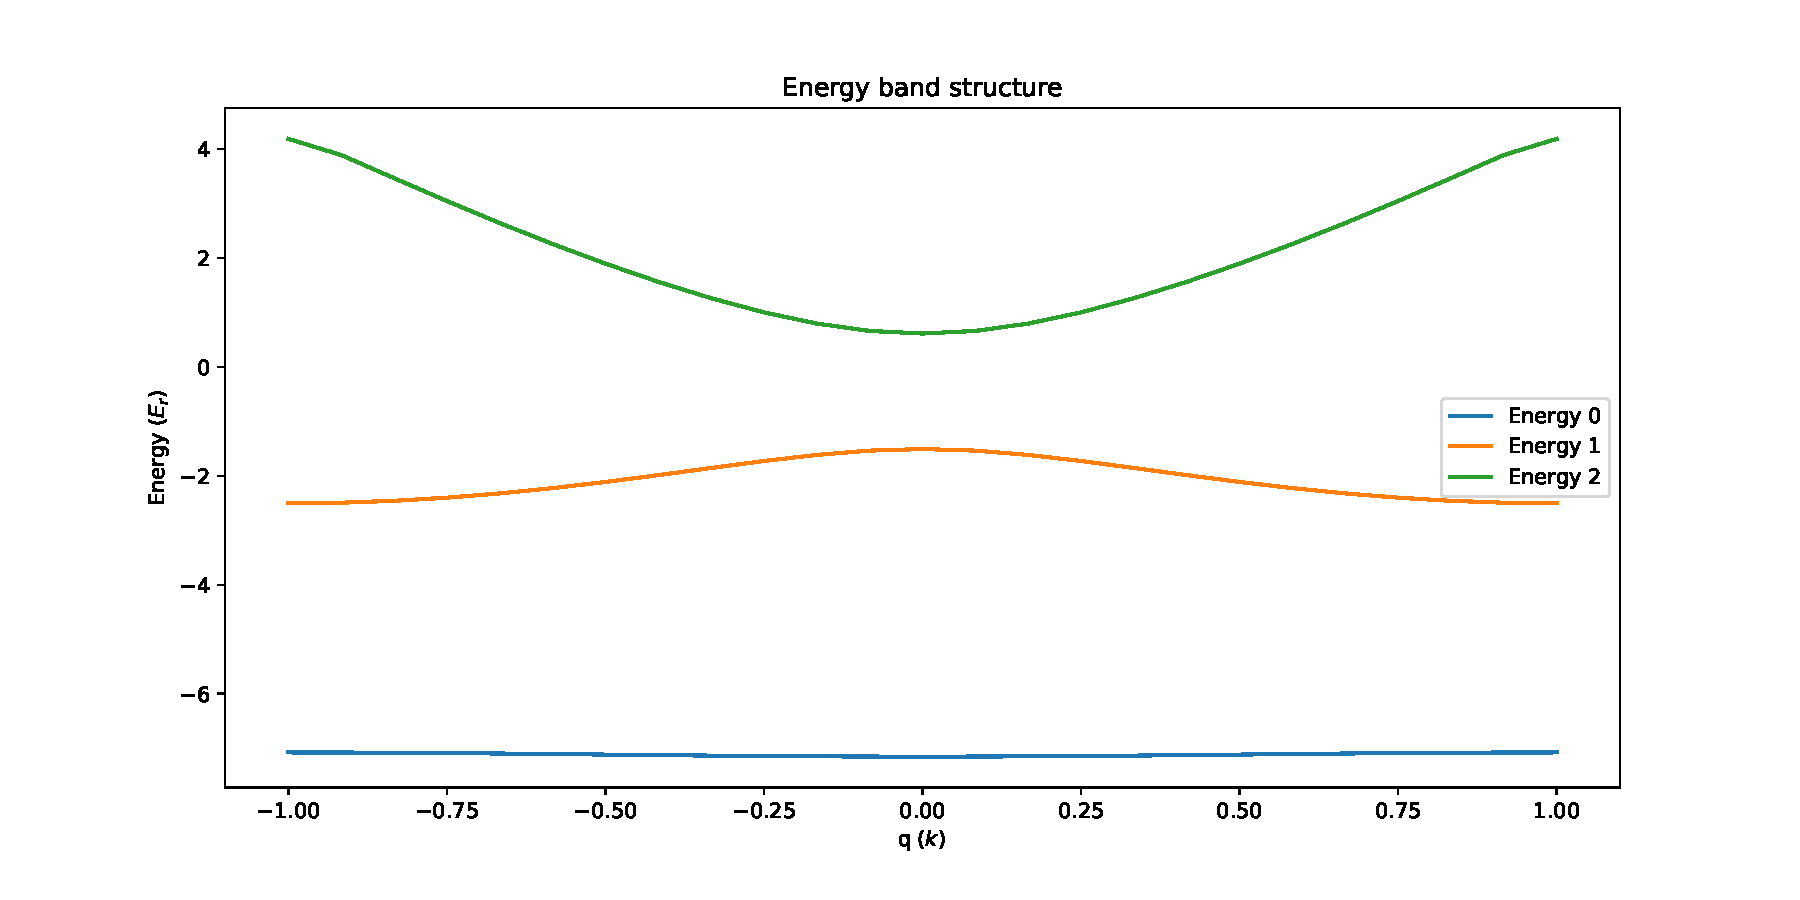
\includegraphics[width=\textwidth]{\figuredir{hopping/band-structure.pdf}}
  \captionsetup{width=.9\textwidth}
  \caption{First three energy bands for an optical lattice depth of
      $V_0=-10E_r$.}
  \label{fig:band_structure}
\end{figure}

In \Cref{fig:band_structure} we visualized the first energy bands for a
lattice depth of $V_0=-10E_r$ from a matrix with dimensions 60.

the coefficients of the Bloch states
\cref{eq:state_bloch_in_reciprocal_lattice} numerically and thereof the
hopping terms using either the exact expression
\cref{eq:element_energy_hopping} over all quasi-momenta $\hbar q$ or through
the tight binding approximation \cref{eq:hopping_amplitude_energies}.

\subsection{Analytical proximity}

The literature \cite{Bloch2008} also reports the analytical proxmity
\begin{equation}
  J^n_1\approx
  \frac{4}{\sqrt{\pi}}\left(\frac{V_0}{E_r}\right)^{3/4}\exp(-2\sqrt{V_0/E_r})
  \label{eq:hopping_proximity}
\end{equation}
to be valid for sinusoidal potentials like \cref{eq:potential_effective} and
to be derived from the Mathieu equation. The Mathieu equation can be obtained
from the time-independent Schrödinger equation with
$V_0\cos^2(kx)=\frac{1}{2}V_0\left(1-\cos(2kx)\right)$. \cite{Connor1984}
gives a more elaborate deviation of \cref{eq:hopping_proximity}.

\subsection{Results}

Comparison of different methods to obtain the hopping amplitude and how
they behave for different potential deeps. Conversion of the hopping term to
a frequency and significance for our experiment.

\chapter{Digital signal synthesis}

The previous chapters have covered the physical theory behind our targeted
application. From that we were able to recover some technical requirements
imposed on our implementation. In this chapter we will review the fundamentals
of digital signal synthesis as \gls{rf} signal source to control the \gls{aod}.

\gls{dds} offer some distinct advantages over traditional analog synthesiser.
For one they can cover up a wide frequency range with high tuning resolution.
In contrast thereto analog devices have to be fitted to a narrow operation
range and are subject to variations caused by aging, thermal drift and
manufacturing. In addition \gls{dds} permit extremly fast, phase-continous
changes of the output signal parameters, without the loop-settling behaviour
known to analog devices. Most recently \gls{dds} can easily be integrated into
existing digital circuits giving rise to a cost-competitive remote
controllable device. Overall these advantages make the \gls{dds} an attractive
solution for our projected application \gls{rf} signal source \cite{ADTutDDS}.

\section{Operating principle}

\Cref{fig:dds_simple_architecture} depicts a flow diagram of the components
that make up a simple \gls{dds}. Given a system clock frequency $f_\text{sys}$
and the desired output frequency $f_\text{out}$ one can derive the phase
accumulator increment
\begin{equation}
  \Delta\varphi
  =
  \lceil\frac{f_\text{out}}{f_\text{sys}}2^N+\frac{1}{2}\rceil
  \label{eq:dds_phase_increment}
\end{equation}
where $N$ denotes the number of bits the phase accumulator can store.
\begin{figure}[ht]
  \centering
  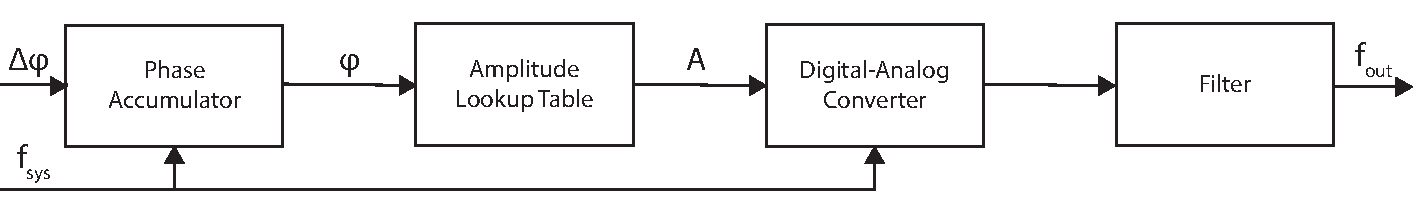
\includegraphics[width=\textwidth]{\figuredir{digital-signal-synthesis/simple-architecture.pdf}}
  \captionsetup{width=.8\textwidth}
  \caption{Signal flow through a simple \gls{dds}. The output frequency
    determines a phase step by which the accumulator is incremented at each
    clock cycle. The value of the phase accumulator is used for amplitude
    lookup of the desired output signal shape. A \gls{dac} outputs the signal
    which then is filtered to smooth the discrete \gls{dac} output.
  }\label{fig:dds_simple_architecture}
\end{figure}
For every clock cycle the phase accumulator is incremented by $\Delta\varphi$.
On overflow of the accumulator a new signal period starts. The phase
accumulator value is used to lookup the corresponding amplitude value of the
desired output signal shape. For example one can use a lookup table with the
values of a sinusoidal output signal. Alternatively one can omit the lookup
table and output a sawtooth output signal by suppling the phase accumulator
output directly to the \gls{dac} or a square wave signal output by suppling
the most significant bit directly. Finally a \gls{dac} converts the digital
amplitude value to an analog signal. An optional analog filter can be used to
smooth the discrete output. In \Cref{fig:dds_simple_output} the signal at the
different processing stages inside a simple \gls{dds} are presented for a
\SI{8}{\bit} precision, system clock frequency
$f_\text{sys}=\SI{1}{\giga\hertz}$ and output frequency
$f_\text{out}=\SI{100}{\mega\hertz}$.
\begin{figure}[ht]
  \centering
  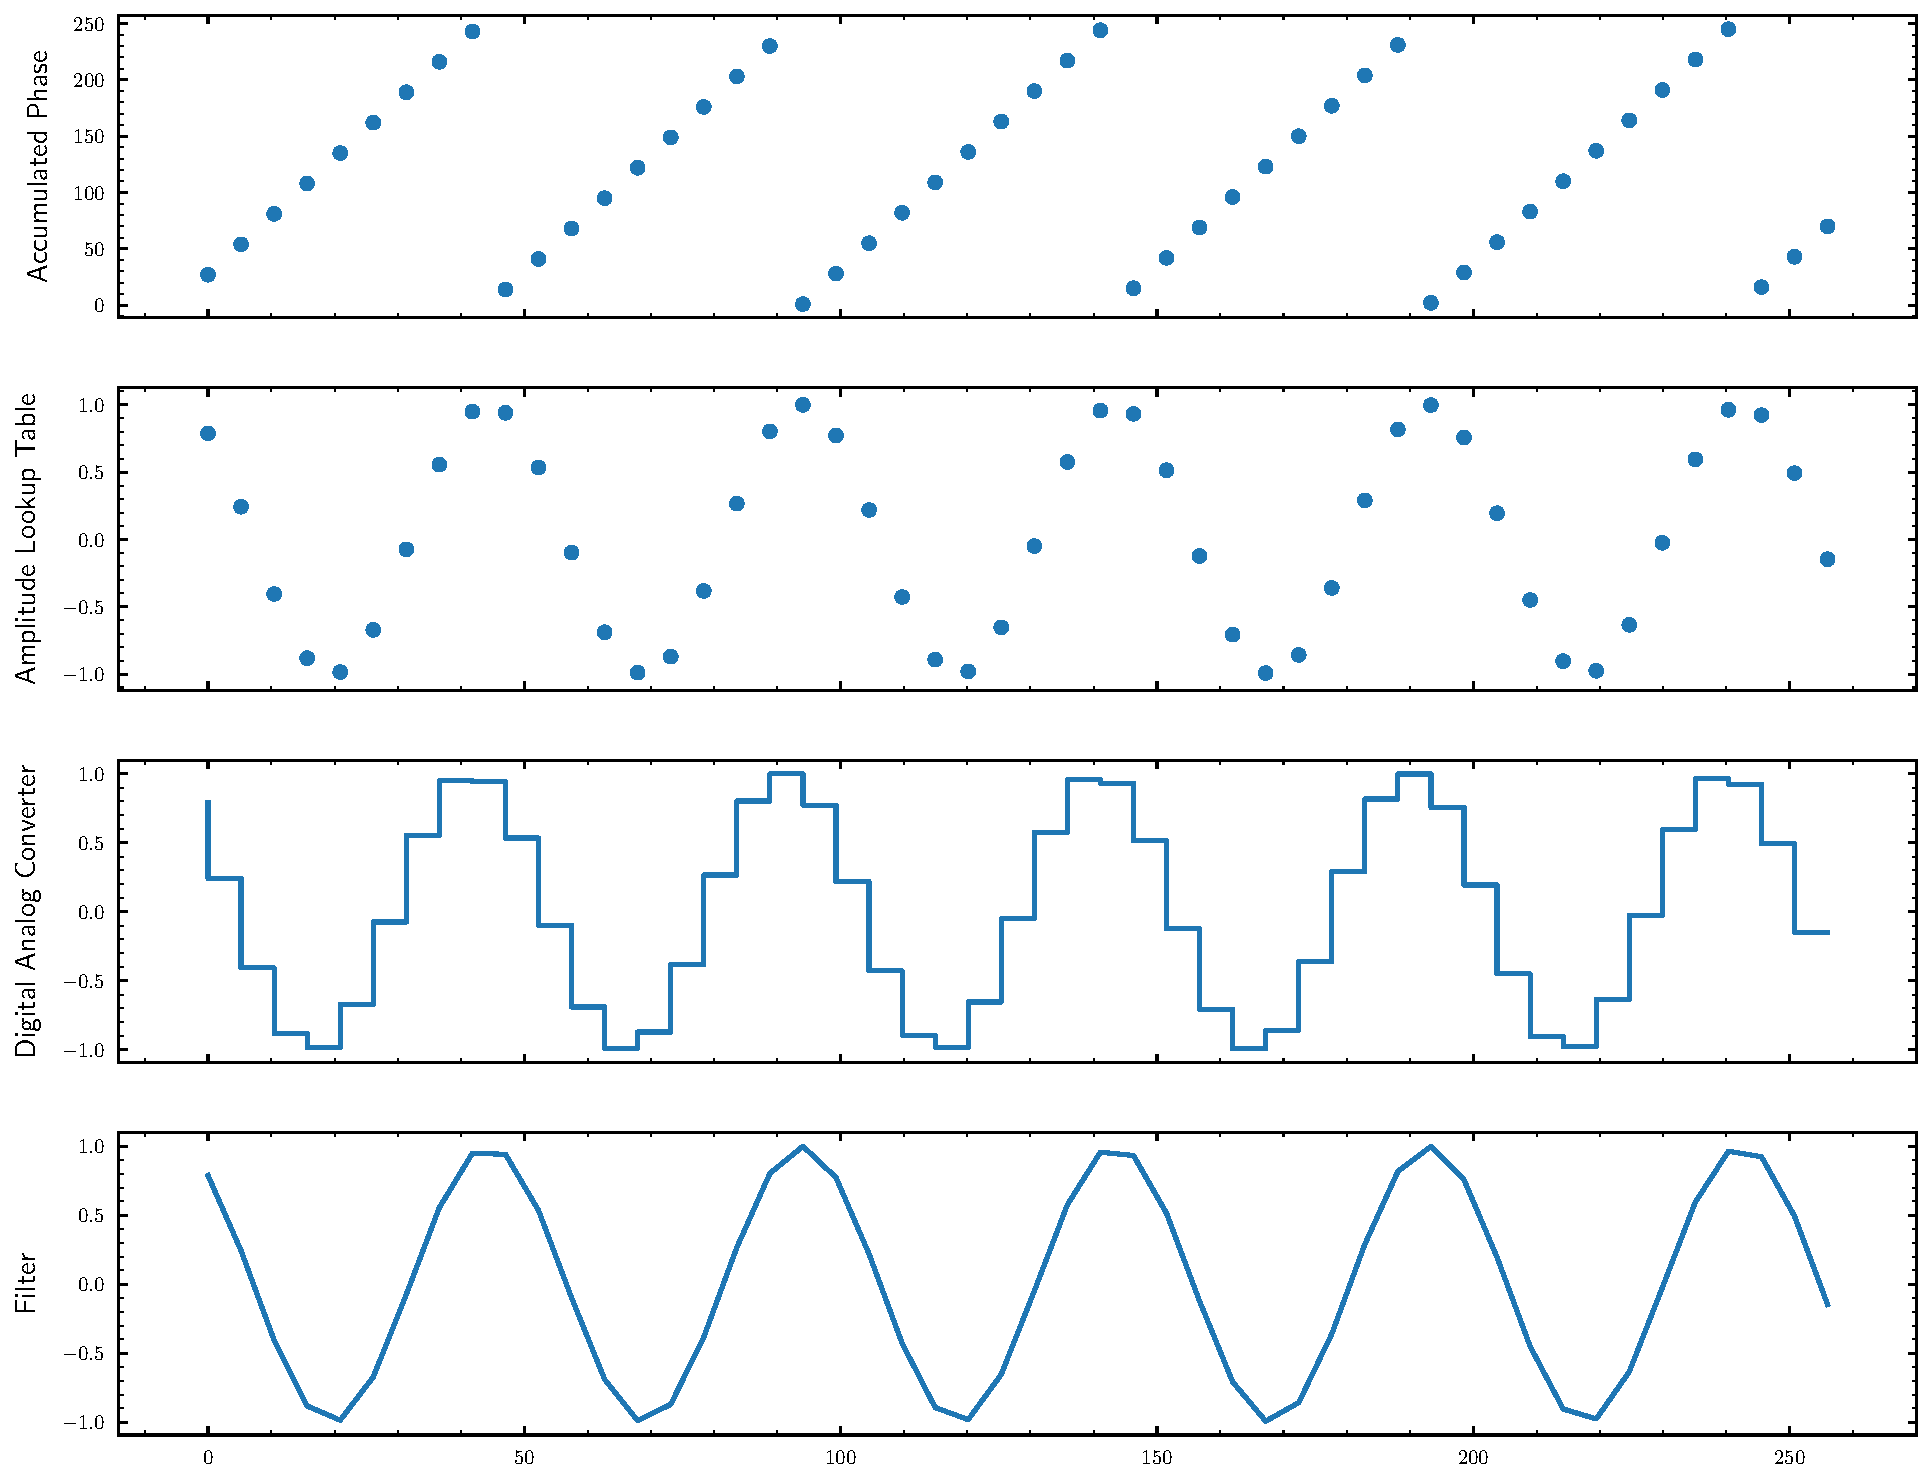
\includegraphics[width=\textwidth]{\figuredir{digital-signal-synthesis/simple-output.pdf}}
  \captionsetup{width=.8\textwidth}
  \caption{Signal outputs at different stages in a simple \gls{dds}. The
    phase accumulator is incremented at each clock cycle by $\Delta\phi$. The
    phase accumulator value is used to lookup a sinusoidal amplitude value
    that is supplied to a \gls{dac}. The final result is smoothed using a
    filter.}\label{fig:dds_simple_output}
\end{figure}
In the first column of \Cref{fig:dds_simple_output} we can see how the phase
accumulator is incremented on every clock iteration and resets on overflow.
In the second column the lookup table has been used to return the
corresponding cosine amplitude. We can see a difference in output shape
between even and odd samples. This is caused by the fact that the phase
increment is not a divisor of the phase accumulator size and we will later
discuss workarounds.

\subsection{Clock generation}

The Nyquist-Shannon sampling theorem states that for a given sample rate a
perfect reconstruction is guaranteed possible for
$f_\text{out}<f_\text{samp}/2$. Until now we have considered the system clock
frequency $f_\text{sys}=f_\text{samp}$ as given. In practice reliable
reference signals are clocked below the desired output range and thereby
cannot directly be used as system clock according to the Nyquist-Shannon
sampling theorem.
\begin{figure}[ht]
  \centering
  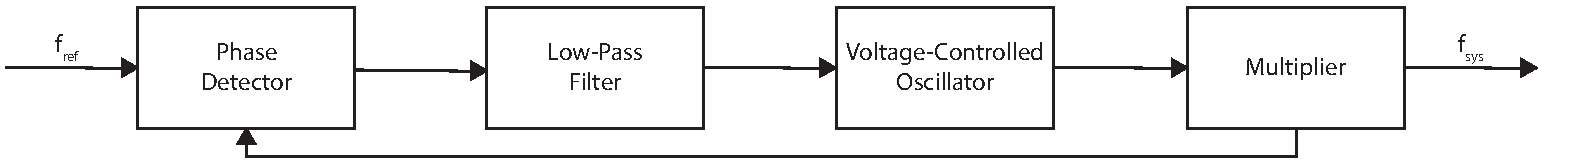
\includegraphics[width=\textwidth]{\figuredir{digital-signal-synthesis/clock-generation.pdf}}
  \captionsetup{width=.8\textwidth}
  \caption{Clock generation signal generation with \gls{pll} and multiplier.
    The phase detector compares the output system phase with the reference
    phase and yields a non-linear error response. The low-pass filter removes
    fast oscillations. The \gls{vco} changes the output phase in dependence
    of the error response. Finally system and reference phase will go in lock.
    }\label{fig:dds_clock_generation}
\end{figure}
\Cref{fig:dds_clock_generation} the system clock generation from a reference
signal is illustrated. The phase detector yields a non-linear error response
comparing the output signal phase with the reference signal phase. After a
low-pass filter removes fast oscillations a \gls{vco} changes its phase
proportional to the error signal. Finally a frequency multiplier creates
harmonics of the reference frequency and extracts a programmed frequency
multiple of $M$ such that the system frequency relates to the reference
clock by $f_\text{sys}=Mf_\text{ref}$ with $1<M\in\mathbb{N}$.

\subsection{Parameter modulation}

So far we only discussed the case of frequency modulation. We will see that
the previous architecture can be easily extended to support amplitude
and phase modulation too.
\begin{figure}[ht]
  \centering
  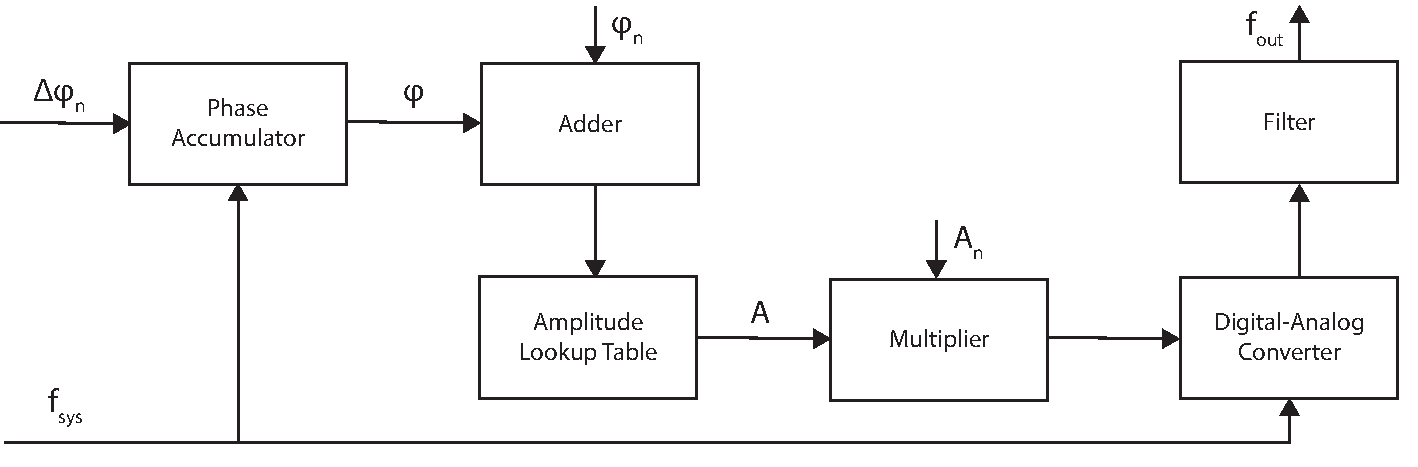
\includegraphics[width=\textwidth]{\figuredir{digital-signal-synthesis/modulation-architecture.pdf}}
  \captionsetup{width=.8\textwidth}
  \caption{
    \gls{dds} architecture supporting modulation of frequency, amplitude and
    phase offset parameters. Phase accumulator increment is now time dependent.
    The phase offset is also time dependent is added as last step to the
    phase accumulator before supplied to the \gls{dac}. The time dependent
    amplitude parameter is multiplied with the amplitude obtained from the
    lookup table.
    }\label{fig:dds_modulation_architecture}
\end{figure}
In \Cref{fig:dds_modulation_architecture} we can see one realization of an
architecture that supports amplitude, frequency and phase modulation. The main
components are the same as in \Cref{fig:dds_simple_architecture}. In addition
we have an adder for a time dependent phase offset and a multiplier for the
digital amplitude value obtained from the lookup table. The time dependence
of the parameters can be either determined by reading from memory or through
generation of another circuit. In a later section we will discuss the case of
a linear frequency sweep provided by a digital ramp.

\section{Quantization errors}
\section{Frequency response}

\section{Operating range}

We apply a reference signal of
\begin{equation}
  f_\text{ref}=\SI{10}{\mega\hertz}
\end{equation}
configured to be used with a \gls{pll} multiplier of
$N=100$ yielding a system clock of
\begin{equation}
  f_\text{sys}=Nf_\text{ref}=\SI{1}{\giga\hertz}.
\end{equation}
The timer clock used for the linear ramp and memory playback runs with
a quarter of the system clock
\begin{equation}
  f_\text{timer}=f_\text{sys}/4=\SI{250}{\mega\hertz}.
\end{equation}

The \gls{ad9910} uses a \SI{14}{\bit} \gls{asf} and \SI{32}{\bit} \gls{ftw}
to parameterize amplitude $A(t)$ and output frequency $f(t)$ by
\begin{align}
  FTW
  :=
  \left\lfloor2^{32}\left(\frac{f_\text{out}}{f_\text{sys}}\right)\right\rceil
  &&
  ASF
  :=
  \left\lfloor\frac{A_\text{out}}{2^{14}}\right\rceil
  \label{eq:elec:ftwasf}
\end{align}
wherein $\lfloor{\cdot}\rceil$ rounds the given float to the nearest integer.
The theoretical limit for the maximum output frequency then is found via
\begin{equation*}
  f_\text{max}
  =
  \left(1-\frac{2^{31}-1}{2^{32}}\right)f_\text{sys}
  =
  \left(\frac{1}{2}-\frac{1}{2^{31}}\right)f_\text{sys}
  \approx
  \frac{1}{2}f_\text{sys}
  =
  \SI{500}{\mega\hertz}.
\end{equation*}
Yet the datasheet \cite{AD9910} reports $f_\text{max}=\SI{420}{\mega\hertz}$
and in fact we found the output signal to be very noisy at the theoretical
limit.

We continue with the assessment of the digital ramp that does a unidrectional
linear sweep on the frequency from \SI{90}{\mega\hertz} to
\SI{110}{\mega\hertz}. The digital ramp of the \gls{ad9910} lets us define
a \gls{ftw} step $M$ word of \SI{32}{\bit} as well as a step rate word $S$ of
\SI{16}{\bit} resolution. They relate to the frequency step and the time
step through
\begin{align}
  \Delta f
  =
  \frac{M}{2^{32}}f_\text{sys}
  &&
  \Delta t
  =
  \frac{S}{f_\text{timer}}
  =
  \frac{S}{4f_\text{sys}}.
  \label{eq:elec:step}
\end{align}
The sweep duration is deterimened by $S,M$ through
\begin{equation}
  T_\text{duration}
  =
  \frac{f_\text{upper}-f_\text{lower}}{\Delta f}\Delta t
  =
  2^{32}\frac{f_\text{upper}-f_\text{lower}}{f_\text{sys}}\frac{S/M}{f_\text{timer}}
\end{equation}
for a target sweep duration of $T_\text{duration}=\SI{10}{ms}$ we find
\begin{equation*}
  \frac{S}{M}
  =
  \frac{T f_\text{timer}}{2^{32}}\frac{f_\text{sys}}{f_\text{upper}-f_\text{lower}}
  =
  \frac{10^9}{2^{35}}
  \approx
  \num{2.9104e-2}
  =
  \frac{1819}{62500}
\end{equation*}
the last step can be obtained by best ratio approximation using continued
fractions as for example described in \cite{Ashley2003}. It should be kept in
mind that the best ratio approximation is likable to introduce an error,
therefore realistic durations may differ from the configured value and it
is possible that better approximations exist that allow smaller $\Delta f,
\Delta t$, thus providing a sweep resolution. In the above case the given
time duration translates to
\begin{align*}
  \Delta f
  =
  \frac{62500}{2^{32}}f_\text{sys}
  \approx
  \SI{145}{\kilo\hertz}
  &&
  \Delta t
  =
  \frac{1819}{f_\text{timer}}
  \approx
  \SI{7.28}{\micro\second}
\end{align*}
or $(f_\text{upper}-f_\text{lower})/\Delta f=138$ discrete data points.

Eventually we are left with the assessment of the amplitude sequence. The
memory fits at most 1024 discrete amplitude values and the \gls{ad9910}
allows us to set the time spent at each amplitude value via the \SI{16}{\bit}
playback rate $P$ word
\begin{equation}
  \Delta t
  =
  \frac{P}{f_\text{timer}}
  =
  \frac{4P}{f_\text{sys}}
\end{equation}
which gives us range from $\min\Delta t=\SI{4}{\nano\second}$ to
$\max\Delta t=\SI{26.14}{\micro\second}$. As we incorporate all of the 1024
data points this gives us a duration range from about
$\min T=\SI{4}{\micro\second}$ to $\max T=\SI{26.84}{\milli\second}$.


\chapter{Experimental setup}

The exerimental setup was largely adopted from \cite{Hertlein2017}, amendments
made include the \gls{rf} signal source of the \gls{aod} and an additional
photodiode to measure the deflected beam intensity.

\section{Optics}

The optical setup can be dissect into a closed first section that reduces
the power of the $\SI{532}{\nano\meter}$ laser source from $\SI{10}{\watt}$
to below $\SI{2}{\milli\watt}$ and an open second section for beam deflection.
Both sections are connected through a \gls{smf}.

\subsection{Power reduction}
\label{sec:powerbox}

Because of safety concerns the power reduction section is confined into a
visually sealed superstructure. \Cref{fig:powerbox} reveals the inside of the
power reduction box.

\begin{figure}[h]
  \centering
  \includegraphics[width=\textwidth]{standalone/powerbox.pdf}
  \caption{Optical configuration of the power reduction section.}
  \label{fig:powerbox}
\end{figure}

The laser beam leaving the laser source is polarized by a $\lambda/2$ retarder
plate such that the succeeding high power beamsplitter BS can divert the
majority of the beams power into a high power beam dump.
Afterwards mirrors M1 and M2 direct the beam towards the center of a $2:1$
telescope composed of two lenses L1, L2 with focal lengths
$f_1=\SI{100}{\milli\meter}$ and $f_2=\SI{50}{\milli\meter}$.
An \gls{aom} diffracts the laser beam into multiple orders. Mirrors M3, M4
project theses orders onto a pinhole which is configured to intromit only the
the first order deflection. The intensity of the first order is subject to
amplitude modulation apllied to the \gls{aom}.
Finally a tunable $\lambda/2$ retarder plate can be used to couple the beam
polarization with the \gls{smf}.

\subsection{Beam deflection and detection}
\label{sec:deflection}

The section for beam deflection and detection as disclosed in
\cref{fig:deflection} receives the down-powered laser beam from previously
described section by a \gls{smf}. Hereinafter the beam passes a tunable
retarder plate and beam splitter BS1. The tunable retarder plate can be used
to adjust the beam intensity without having to access the power box.
A second polarizer with cube BS2 is used to branch off a part of the beam
to a photodiode PD1 that is positioned to be at the focal point of lens L1.
Photodiode PD1 is connected via a control system with the amplitude
modulation of the \gls{aom} depicted in \cref{fig:powerbox} to stabilize
the laser intensity against i.e. thermal drifts.

\begin{figure}[h]
  \centering
  \includegraphics[width=\textwidth]{standalone/deflection.pdf}
  \caption{Optical configuration of the beam deflection section.}
  \label{fig:deflection}
\end{figure}

For horizontal and vertical beam deflection two \gls{aod}s are used. A $1:1$
telescope comprised of two lenses L2, L3
each with focal length $f_2=f_3=\SI{250}{\milli\meter}$ projects the beam
on a pair of objectives that are built of lenses L4 to L7. The purpose of the
objective pair is to focus the laser on to the atom plane.
Consecutively the laser is reflected by a pair of mirrors M3 and M4 to the
part intended for detection. Lens L8 acts as a camera lens and projects the
beam to infinite focus on to the CCD camera sensor. Cube BS3 forks a portion
of the beam away from the CCD camera on to mirror M5 that guides the beam
towards lens L9 in order to focus the beam onto a second photodiode PD2.

\section{Electronics}

Beforehand we described the optical setups used. Now we want to emphasize
on the electronics how they are integrated into the optical setup.

\subsection{Signal source}

The requirements placed by the two \gls{aod} demand flexible but precise
\gls{rf} sources. Fortunately we can resort to a custom made signal
sources based on the \gls{ad9910} \gls{dds} \cite{AD9910} \gls{ic} that can
operate up to \SI{420}{\mega\hertz} and allows modulation of amplitude,
frequency and phase offset by either a constant value or through a single
digital ramp or playback from a memory sequence.

The signal output of the \gls{dds} is of the form
\begin{equation}
  U(t)=A(t)\sin(2\pi f(t)+\phi(t)).
  \label{eq:dds:signal}
\end{equation}
In the following we will ignore the unsynced phase offset, thus setting
$\phi=0$. In case of the single \gls{dds} which drives the \gls{aom} we
have a constant signal, in that sense we can set $A=1$ and
$f_\text{aom}=\SI{80}{\mega\hertz}$ on \cref{eq:dds:signal}.
In the case of the two \gls{dds} which drive the horizontal and vertical
\gls{aod} we configure the frequency to be controlled by the digital ramp in
order to do a linear frequency sweep from
$f_\text{lower}=\SI{90}{\mega\hertz}$ to
$f_\text{upper}=\SI{110}{\mega\hertz}$, yielding
\begin{align}
  f_\text{aod}(t)
  =
  f_\text{lower} + \frac{f_\text{upper}-f_\text{lower}}{T_\text{duration}}t
\end{align}
wherein $T_\text{duration}>0$ denotes the sweep duration. The amplitude is
controlled by memory playback. Given a discrete set of amplitude values
$A_i\in[0,1]$ with $i=1,\dots,N=1024$ the amplitude of the \gls{aod} can be
formulated as
\begin{align}
  A_\text{aod}(t)
  =\sum^N_{i=1}A_i\mathbb{1}_{B_i}(t)
  &&
  B_i:=\left[iT_\text{interval}, (i+1)T_\text{interval}\right[
\end{align}
wherein $T_\text{interval}>0$ denotes the playback interval and
$\mathbb{1}_{B_i}$ is the characteristic function on the set $B_i$.

So far we have assumed $f_\text{aod}(t)$ to be continous and
$T_\text{interval},T_\text{duration}>0$ to be arbitrary, however the internals
of the \gls{ad9910} impose theoretical restrictions on the possible operating
ranges.

\subsection{Signal amplifier}

We use three signal amplifiers with respective input from the signal sources
to have an output power of about $P=\SI{2}{\watt}$ required by the \gls{aod}s
and \gls{aom} for ideal operation. The used amplifiers offer a second input
for external amplitude modulation. In case of the \gls{aom} we connect this
input with the intensity controller.

\subsection{Intensity controller}

The intensity controller is connected to photodiode PD1 that converts the
laser intensity to an input voltage signal of the controller. Given the
input signal we can configure the controller for a reference input voltage.
The controller will then compare the input voltage with set reference voltage
and output an error signal that is proportional to the deviation of the
input from the reference voltage. The inverted error signal is feed to the
signal amplifier connected with the \gls{aom}.

In one attempt we tried to use the intensity controller to compensate for
frequency dependent intensity changes during frequency sweep of the \gls{aod},
however we found that even slow sweep times of $\SI{2}{\second}$ could not
be balanced, therefore the intensity controller only compensates for slow
intensity shifts caused by thermal stress of the laser source.

The intensity controller has to be connected correctly with photodiode PD1
of the setup as well as signal amplifier of the signal that drives the
\gls{aom}.

\begin{figure}[h]
  \centering
  \includegraphics[height=6cm]{example-image-a}
  \caption{The intensity controller next to the \gls{aom} amplifier.}
  \label{fig:intcontrol}
\end{figure}

The XY can be tuned to set the reference signal.

\subsection{Trigger source}

To syncronize the signal sources, the \gls{ccd} camera and the oscilloscope
it was necessary to design a global trigger source that outputs a rising edge
signal to multiple devices and exposes a network programable interface.

\begin{figure}[h]
  \centering
  \includegraphics[height=6cm]{example-image-a}
  \caption{The trigger source exposes a network programable interface and
  provides enough power to drive four output signals.}
  \label{fig:elec:trig}
\end{figure}
The schematics and board layout can be found in the
\cref{app:electronics:trigger_hub}.

\section{Acousto-Optics}

\subsection{Modulator}
\subsection{Deflector}

\section{Assessment}

With the previously described calibration steps in place we can assess the
final quality of the beam with an image capture of the \gls{ccd} camera in the
aligned setup \cref{sec:deflection}.

\begin{figure}[ht]
  \centering
  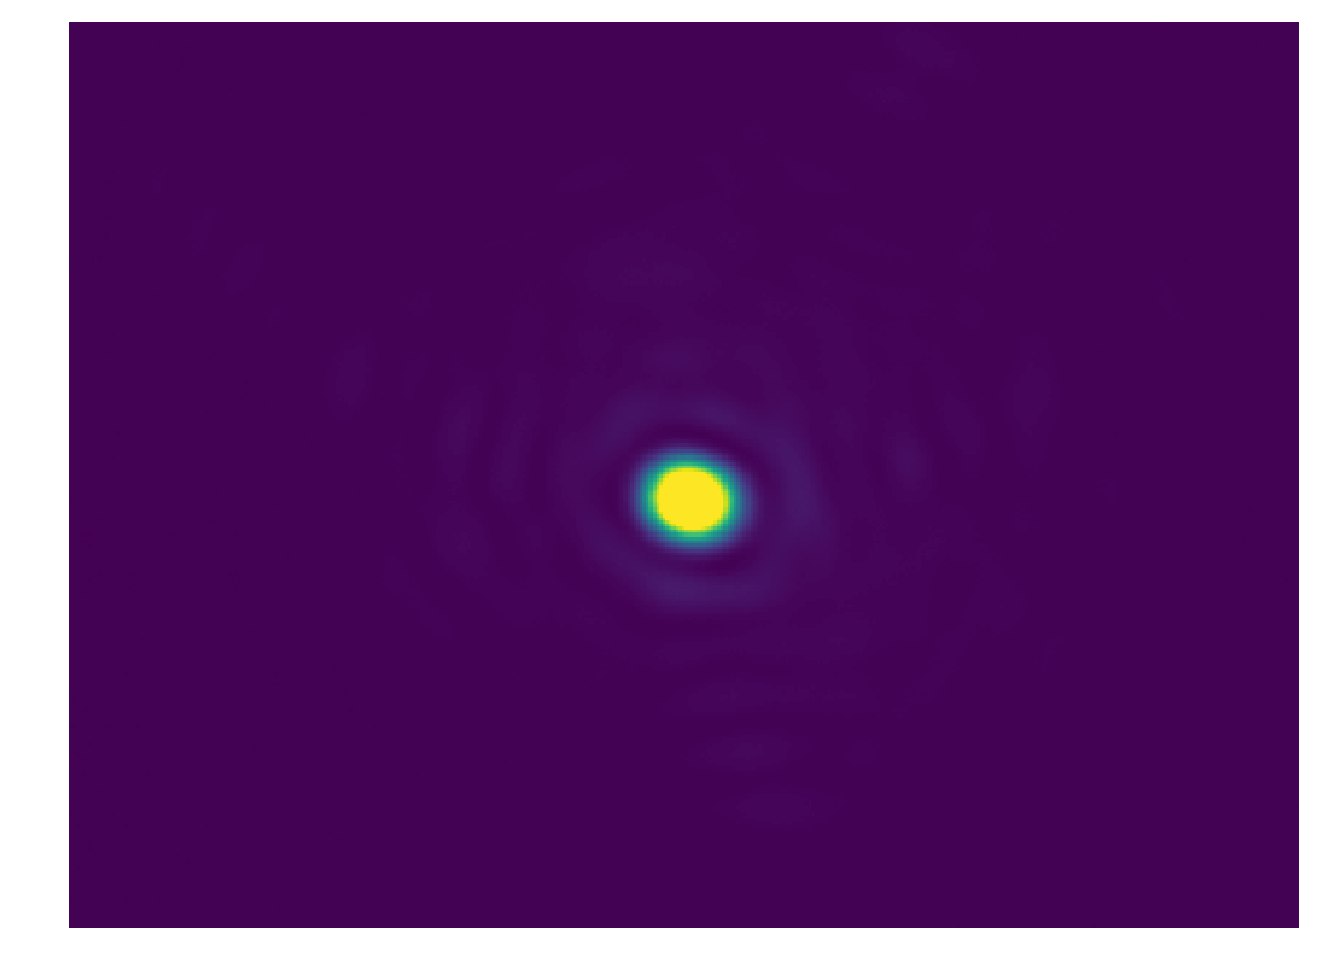
\includegraphics[width=.5\textwidth]{\figuredir{camera/profile2d.pdf}}
  \caption{Image detail from the captured beam with the \gls{ccd} camera.}
  \label{fig:beamprofile:2d}
\end{figure}

The two dimensional beam profile shows the characteristical two dimensional
gaussian distribution with diffraction rings caused by beam clipping at
finite apertures as described in \cite{Hertlein2017}.

\begin{figure}[ht]
  \centering
  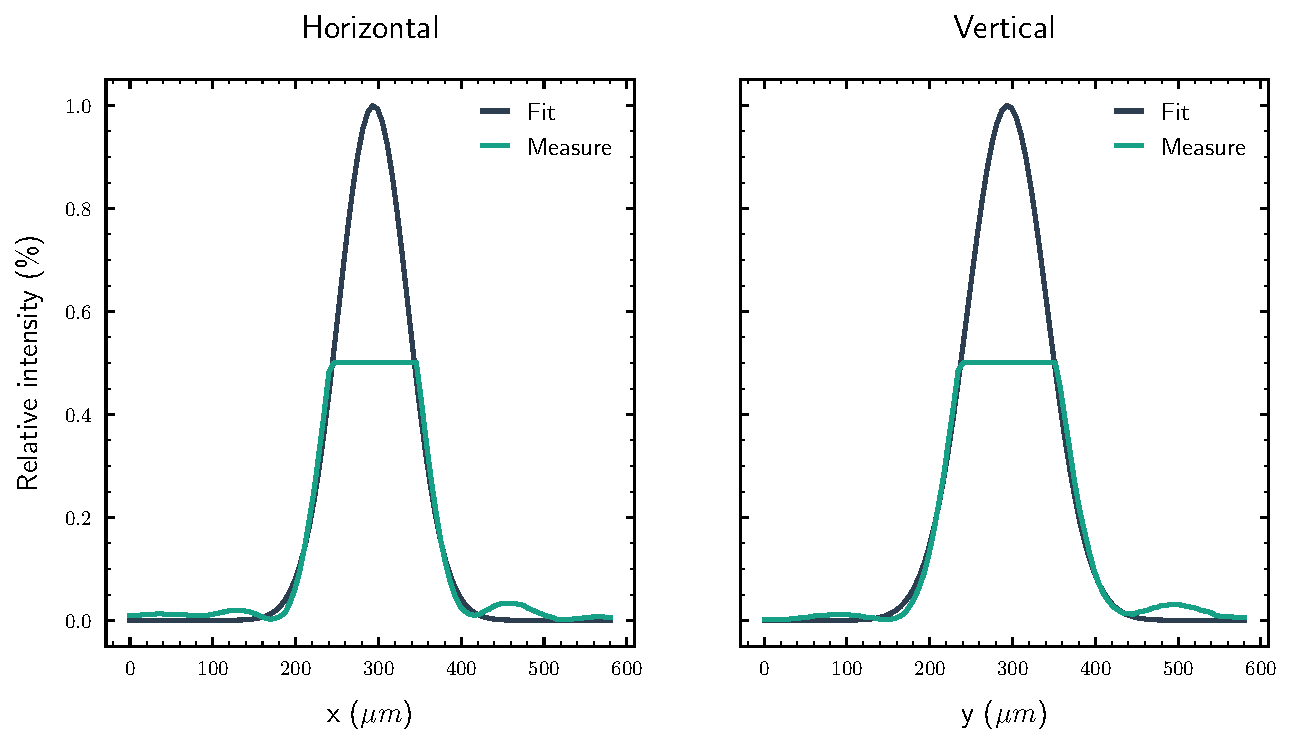
\includegraphics[width=\textwidth]{\figuredir{camera/profile1d.pdf}}
  \caption{1D horizontal and vertical profile extracted from the center of
    the image detail in \cref{fig:beamprofile:2d} with fitted gaussian curve
  and residue.}
  \label{fig:beamprofile:1d}
\end{figure}

By inspecting the one dimensional profiles with fitted gaussian and residue
we again confirm conclusions drawn in \cite{Hertlein2017}. The clipped top
of the measured intensity originates from the saturated pixels of the
\gls{ccd} camera and can be ignored. We further observe a slight assymmetry
at the diffraction rings. Overall the shown profiles can be considered to
confirm a good alignment.

\chapter{Characterisation of the electronic setup}

\textit{By the time the \gls{rf} signal has reached the acoustic transducer,
it has been synthesized from a reference signal, amplified, and matched to
the impedance of the \gls{aod} transducer. We are going to inspect the
\gls{rf} signal characteristics at each transmission and find that each stage
unintentionally carries out frequency dependent amplitude characteristics
which, as we will see in the next chapter, are responsible for the complex
intensity distribution observed with the photodiode.}

\section{Digital signal synthesizer}

We already covered the fundamental functionality of the \gls{dds} in
\cref{ch:digital_signal_synthesis} and its integration in our experimental
setup in \cref{subsec:setup_signal_source}, yet we are missing physical
measurements of the frequency and the amplitude characteristics.

Physical analysis of the \gls{dds} output \gls{rf} signal is in fact no simple
endeavour as usual operation time scales are of many magnitudes greater than
the signal periodicity. The strategy we used to resolve this circumstance is
depcited in \Cref{fig:signal_window}.
\begin{figure}[ht]
  \centering
  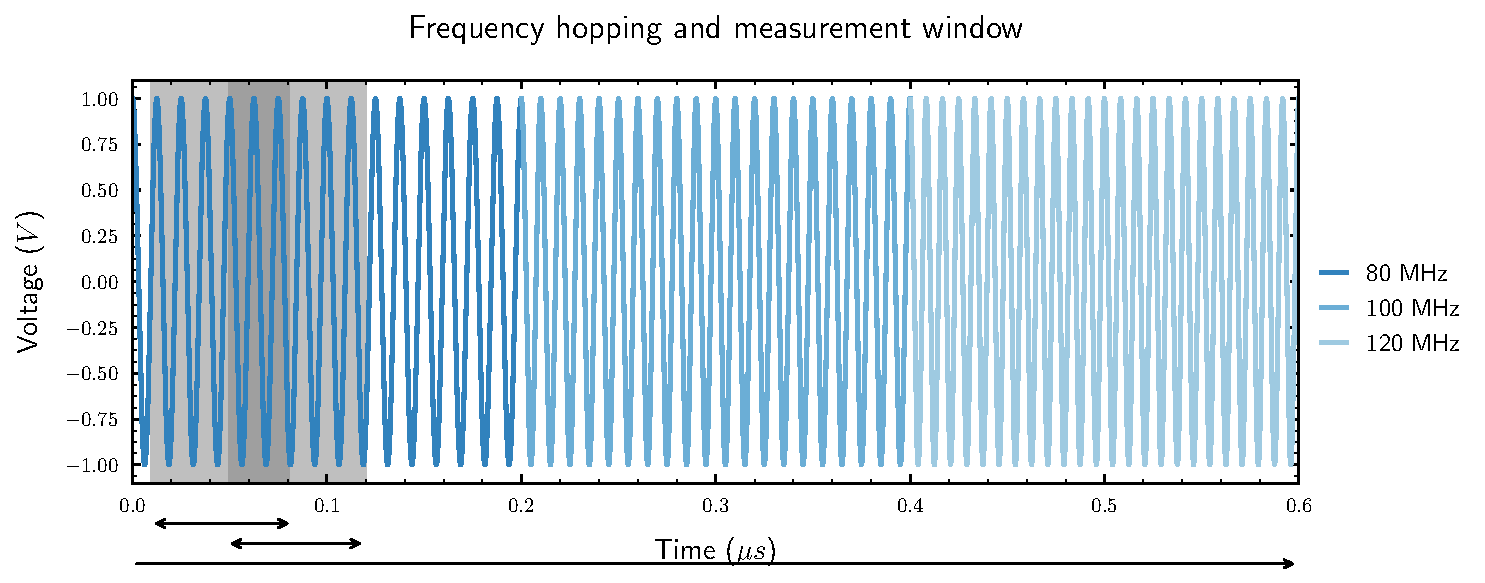
\includegraphics[width=\textwidth]{\figuredir{signal/window.pdf}}
  \captionsetup{width=.9\textwidth}
  \caption{Idealized \gls{dds} signal output with constant frequency
    increments. The measured window only captures a subset (gray) of the complete
    modulation (shades of blue).}\label{fig:signal_window}
\end{figure}
The strategy consists of capturing multiple, small time windows of the signal
(gray) which delayed would cover the complete signal trace (blue).
\begin{figure}[ht]
  \centering
  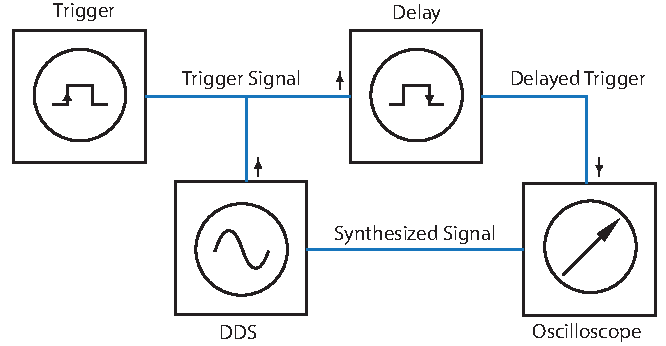
\includegraphics[width=.8\textwidth]{\figuredir{signal/setup-dds.pdf}}
  \captionsetup{width=.8\textwidth}
  \caption{Measurement setup of the synthesiyer signal. By inserting a pulse
    generator in between the trigger source and the oscilloscope we can delay
    the capture window of the oscilloscope by the pulse width.
  }\label{fig:signal_window_setup}
\end{figure}
The experimental setup used to reailize this concept is schematically drawn in
\Cref{fig:signal_window_setup}. In between the oscilloscope and the trigger
source we inserted a pulse generator. The pulse generator width equals the
delay time of the oscilloscope as the oscilloscope is configured to capture
on the falling edge signal of the pulse generator. Further the oscilloscope's
impedance was configured to \SI{50}{\ohm}. High impedance measurements at
such frequencies causes very different behaviour as the electromagnetic wave
is reflected subject to the actual frequency inside the coaxial cable. In 
\Cref{tab:signal_parameters_dds} we can find an overview of the experimental
parameters used.
\begin{table}[h]
  \centering
  \begin{tabular}{|c|c|c|c|c|c|}
    \hline
    Frequency Range $f$ &
    Sweep Duration $T_s$ &
    Window Duration $T_w$ &
    Number Windows $N_w$ \\
    \hline
    \SIrange{80}{120}{\mega\hertz} &
    \SI{30}{\milli\second} &
    \SI{50}{\micro\second} &
    300 \\
    \hline
  \end{tabular}
  \captionsetup{width=.8\textwidth}
  \caption{Experimental parameters used to inspect the output \gls{rf} signal
  of the \gls{dds}.}
  \label{tab:signal_parameters_dds}
\end{table}
The specified frequency range is motivated to cover the greatest possible
spatial dimensions permitted by the dimensions of the optics. Sweep and
window duration where selected as a compromise between the oscilloscope being
able to resolve the signal fine enough to perform \gls{fft} and the sweep
duration being comparable to later experiments. Time delay was incremented
in $N_w$ steps until $T_s=T_w$, thus we will capture $N_w$ overlapping windows.

\subsubsection{Frequency spectrum}

For an ideal linear frequency sweep we would expect a continous increase of
the frequency with respect to time, yet we know that \gls{dds} makes use of
digital signal processing methods which suggests a discrete frequency
spectrum. To help us expose the characteristics of the digital frequency
sweep we will utilize a spectrogram. A spectrogram visualizes how the
frequency spectrum varies in time. One way to obtain a spectrogram is to
partition the data into overlapping time chunks while performing \gls{fft}
which allows us to combine time and frequency domain specific
characteristics. In our case we choose the relative spectral power to be
encoded through color.
\begin{figure}[ht]
  \centering
  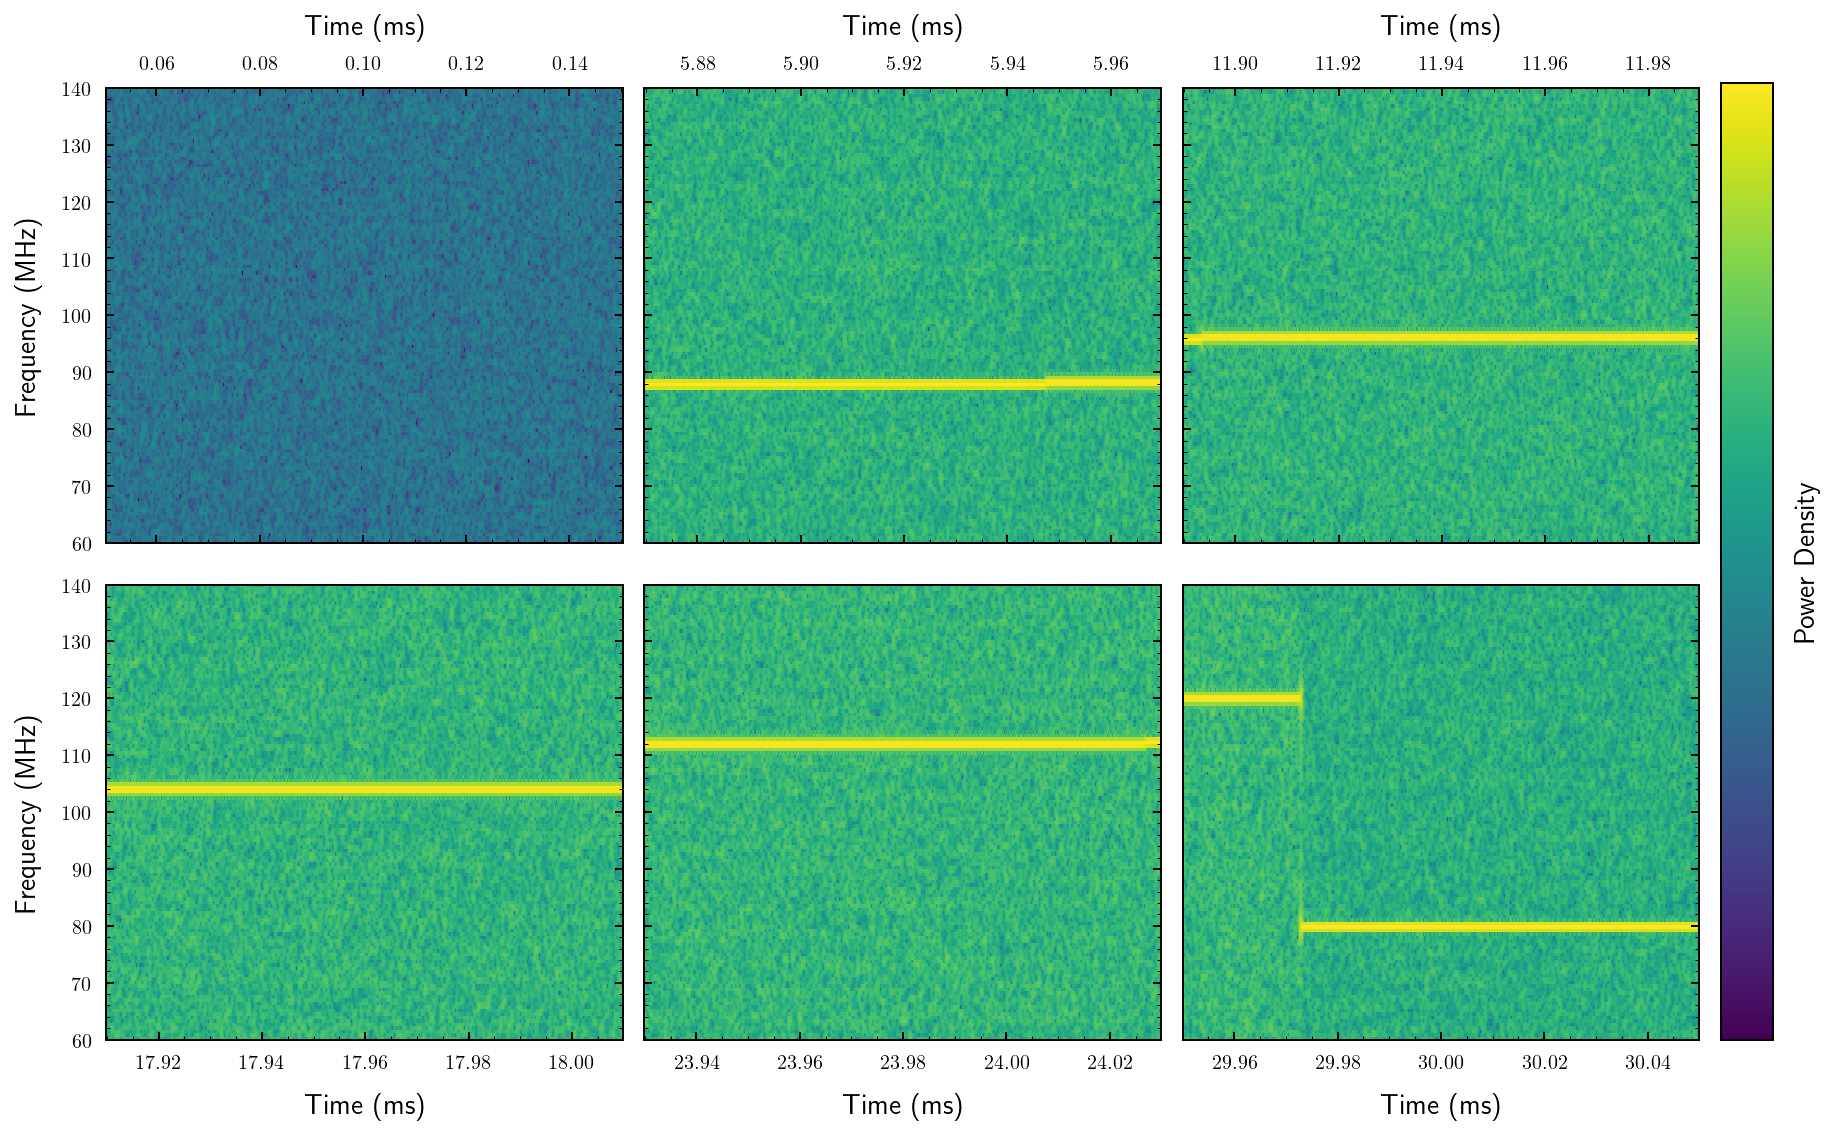
\includegraphics[width=\textwidth]{\figuredir{signal/synthesis/spectrogram.png}}
  \captionsetup{width=.8\textwidth}
  \caption{Spectrogram of delayed time windows of the \gls{dds} output signal
    configured to perform a linear frequency sweep. For an ideal linear sweep
    we would expect a linear timeline of the frequency, instead we observe a
    discrete set of frequencies.}
  \label{fig:signal_synthesis_spectrogram}
\end{figure}
\Cref{fig:signal_synthesis_spectrogram} depicts four spectrograms, each taken
at a different time window of the frequency sweep passthrough. The first
spectrogram captures the start of the frequency sweep as can be read from
the time scale. The first time window does not disclose any signal. This
phenomena will be observed frequently. For unknown reasons the output signal
of the \gls{dds} is absent for multiple microseconds after the \gls{dds}
receives the external trigger signal. The exact duration of the trigger hole
varies but does not affect the internal state of the \gls{dds} as the first
measured frequency matches the theoretically expected frequency according to
the ramp. If we take a look at the following spectrogram windows we can see
how the \gls{dds} outputs a constant frequency over a short time period,
therefore the frequency range consists of discrete frequencies. We can
actually even observe such a frequency increment in the second, third and
fifth spectrogram. Finally in the last spectrogram the frequency drops back
to the initial value - a side effect of the \gls{dds} sweep mode which
supports an external trigger signal.

\subsubsection{Amplitude frequency response}

In the Fourier space we can locate the dominant frequency at the maximum of
the power spectrum. That in mind we can reduce the previous obtained time
window measurements to pairs of dominant frequencies and maximum amplitude.
Under the assumption that the maximum voltage per measurement is approximately
the mean peak-to-peak amplitude of the signal - which during the oscilloscope
suggested during measurements - we can find the amplitude frequency response
spectrum with manageable effort. \Cref{fig:signal_synthesis_response}
visualizes the described routine for the \gls{dds} assigned to the \gls{h} and
\gls{v} \gls{aod} with frequency control by digital ramp and manual increments.
\begin{figure}[ht]
  \centering
  \includegraphics[width=.9\textwidth]{\figuredir{signal/synthesis/response.pdf}}
  \captionsetup{width=.9\textwidth}
  \caption{Amplitude frequency response of the \gls{dds} signal sources for
    the \gls{h} and \gls{v} \gls{aod}. The frequency increments
    are performed through the integrated digital ramp and manually.
  }\label{fig:signal_synthesis_response}
\end{figure}
The peak-to-peak amplitude of the synthesizser signal is constant with small
noise contribution. On a closer view we can see that the oscilloscopes voltage
resolution is at its limit, thus we only observe discrete voltage steps.
We therewith conclude from \Cref{fig:signal_synthesis_response} that the
amplitude response of the \gls{dds} is independent of the output frequency
and the method used to provide frequency increments. The inverse sinc response
we theorized in \cref{ch:digital_signal_synthesis} is not observable in the
measured frequency range as \SI{100}{\mega\hertz} are a fraction of the
Nyquist frequency \SI{1}{\giga\hertz} used for sampling inside the \gls{dds}.

\section{Power amplifier}

The piezoelectric attached to the acousto-optic crystal inside the \gls{aod}
elements has to emit acoustic waves strong enough to propagate through the
crystal of the \gls{aod}. The power demands specified by the \gls{aod} are
not met by the \gls{dds}, therefore we have to employ a power amplifier
between the \gls{dds} and \gls{aod}. Even though we previously concluded that
the \gls{dds} signal amplitude is independent of the output frequency, the
power amplifier can introduce new frequency dependent characteristics which
we dedicate ourselves to.

\subsubsection{Amplitude frequency response}

The measurement procedure described in the previous section is still valid
for the now amplified signal of projected \SI{33}{\decibel\meter}. At the
usual \SI{50}{\ohm} in between coaxial cables this corresponds to an
approximate voltage of \SI{10}{\volt}. In order to protect the oscilloscope
against potential damage caused by too much power, we inserted a chain of
attentuators (order given from coaxial cable to oscilloscope):
\begin{inparaenum}
  \item \SI{1}{\decibel}
  \item \SI{3}{\decibel}
  \item \SI{3}{\decibel}
  \item \SI{6}{\decibel}
  \item \SI{10}{\decibel}
  \item \SI{10}{\decibel}
\end{inparaenum}
The order was chosen in such a way to distribute heat dissipation uniformly
accross the attentuators. The total damping of this configuration yields
\SI{33}{\decibel} which should give us the same signal power from the
\gls{dds}. \Cref{fig:signal_amplification_frequency_max_amplitude} presents us
the damped output signal subject to the signal frequency after amplification
for the two distinct (\gls{h}, \gls{v}) amplifiers and \gls{dds} signals.
\begin{figure}[ht]
  \centering
  \includegraphics[width=.9\textwidth]{\figuredir{signal/amplification/response.pdf}}
  \captionsetup{width=.9\textwidth}
  \caption{Amplitude frequency response of the \gls{dds} signal after power
    amplification. In comparison to the \gls{dds} we observe very small
    oscillations.
  }\label{fig:signal_amplification_response}
\end{figure}
In comparison to the \gls{dds} response the amplifier introduce small ripple
around about \SI{97}{\mega\hertz} and \SI{107}{\mega\hertz}. Further we note
a small constant offset between the \gls{h} and \gls{v} amplifier. We also
cannot identify significant differences between the type of frequency
increment used. Despite these effects are small in terms of voltage it is
difficult to relate them to the overall power response as only voltage but
not current was measured.

\subsubsection{Network analyzer transmission}

We previously discovered that the amplifier amends the frequency amplitude
response, nevertheless it is difficult to isolate the actual influence of
the amplifier and to preclude interaction effects caused by the already
unideal \gls{dds} signal. Therefore we conducted more detailed measurements
of the amplifiers power transmission with the network analyzer. The network
analyzer is a device that can measure reflection and transmission parameters
of electric components and does provide a cleaner input signal then used in
the previous measurement. As in the measurement with the oscilloscope we also
have to protect the network analyzer against the output power of the
amplifier. This time we used a single \SI{30}{\decibel} attentuator in between
the network analyzer input and the power amplifier output.
\begin{figure}[ht]
  \centering
  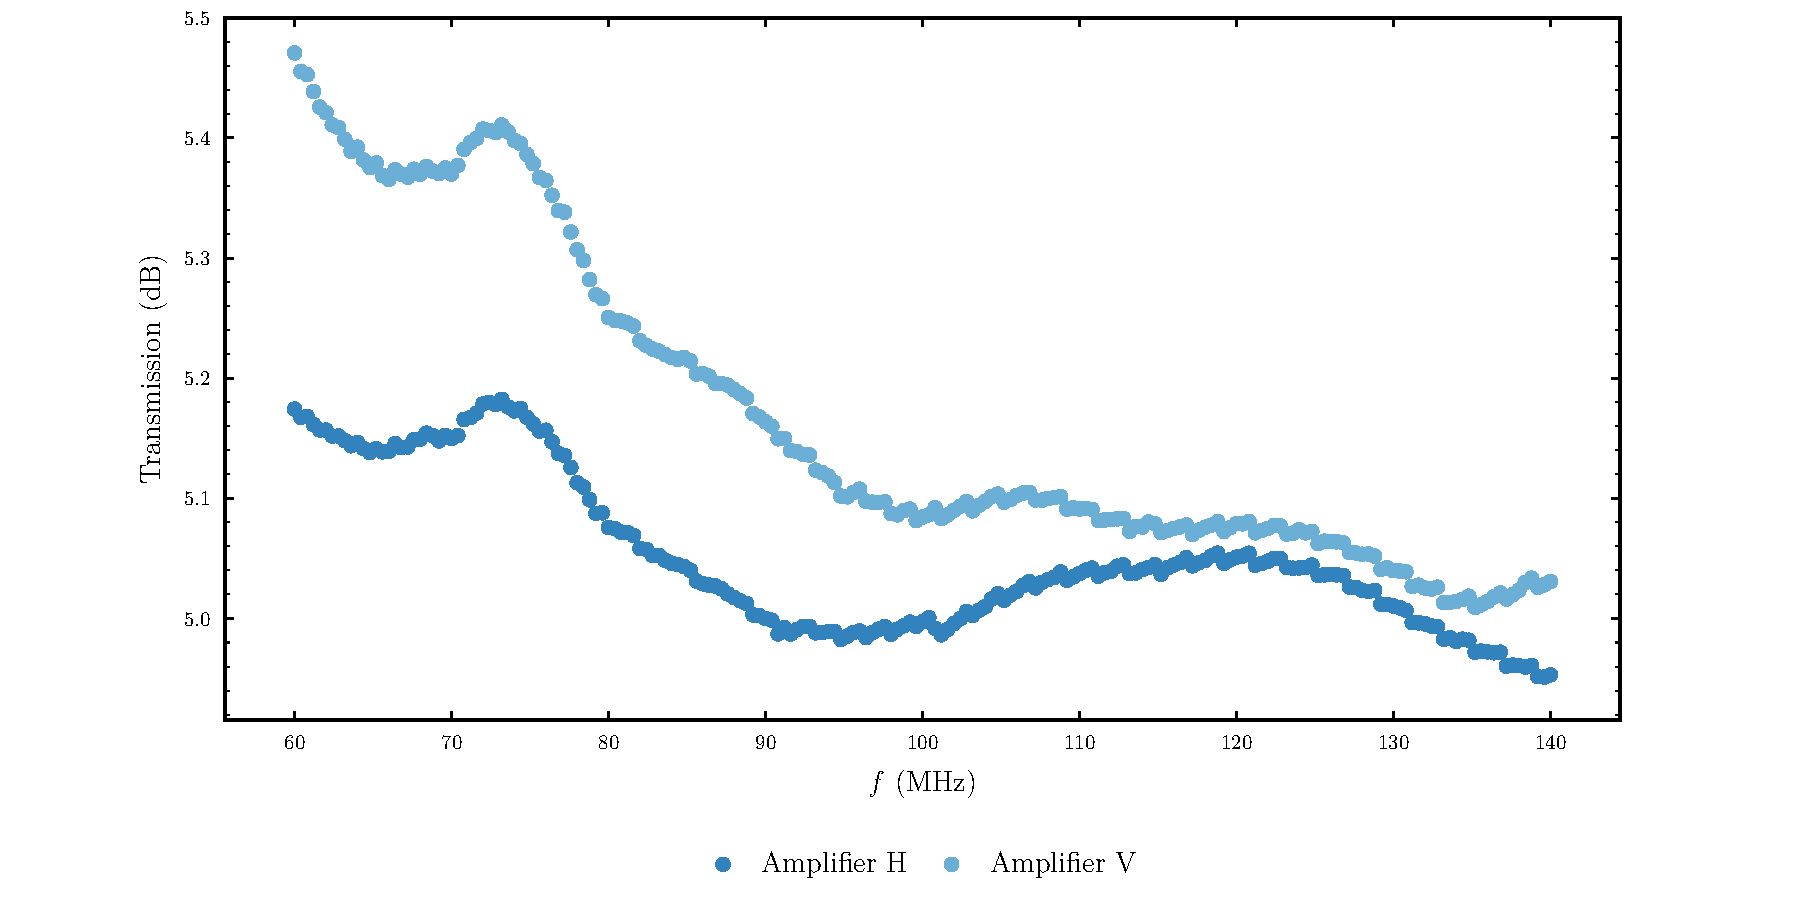
\includegraphics[width=.9\textwidth]{\figuredir{signal/amplification/transmission.pdf}}
  \captionsetup{width=.9\textwidth}
  \caption{Frequency transmission spectrum obtained via the network analyzer
  of the horziontal and vertical amplifiers.}
  \label{fig:signal_amplification_spectrum}
\end{figure}
In \Cref{fig:signal_amplification_spectrum} we see the frequency transmission
spectrum obtained through the network analyzer connected to the horizontal
and vertical amplifiers. We can confirm a fixed offset of the amplification
gain between both amplifiers. If we take a assume a power amplification
difference of $L=\SI{.2}{\decibel}$, i.e.\ between \SI{80}{\mega\hertz} and
\SI{115}{\mega\hertz} with the \gls{v} amplifier, according to
\begin{equation}
  P
  =
  P_010^{L/\SI{10}{\decibel}}
  \label{eq:power_gain_decibel}
\end{equation}
and $P_0=\SI{2}{\watt}$ we would have to expect a drop of up to
\SI{.05}{\watt} in power. Unfortunately we cannot say in how far this is
a relevant magnitude for the \gls{aod}.

\section{Acoustic transducer}

In the previous sections we explored the signal transfer at the synthesis
and amplification stage. The last stage that is accessable to us without
destruction of the \gls{aod} concerns the power reflection at the \gls{aod}
itself. From the reflection we may estimate power transmission
characteristics, hence for a large reflection we would expect a small
transmission and in that sense less beam intensity in the first deflection
order.

\subsection{Reflection spectrum}

The power reflection measurements were conducted with the network analyzer
we already introduced on the power amplifiers. In a first embodiment of the
experiment we directly supplied the \gls{aod} through a coaxial cable of the
network analyzer with power and measured the reflection. In a second
embodiment we used a direct-coupler to supply the respective amplifier with a
signal and measure the reflection through a direct-coupler.

\subsubsection{Direct connection}

\Cref{fig:signal_reflection_direct} visualizes the power reflection spectrum
of both \gls{aod} elements when directly connected to the network analyzer at
a maximum output power of \SI{10}{\decibel\meter}.
\begin{figure}[ht]
  \centering
  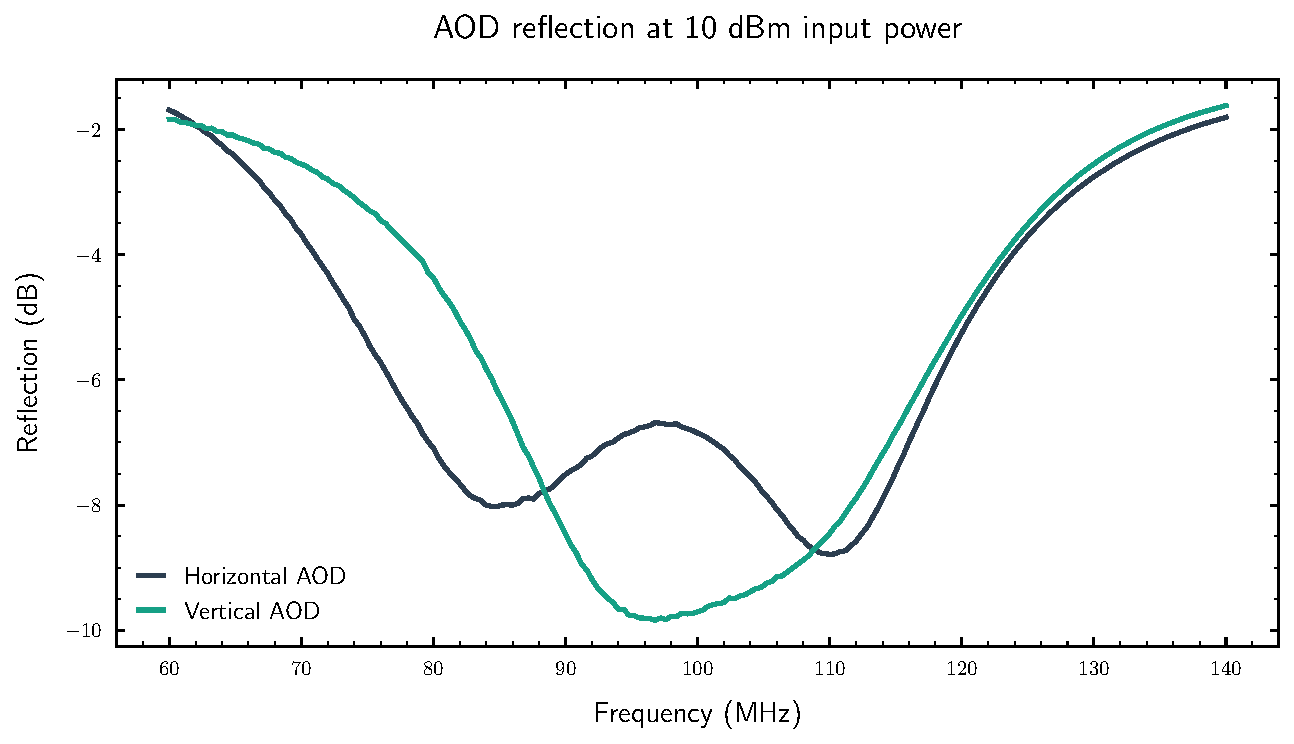
\includegraphics[width=.9\textwidth]{\figuredir{signal/reflection/direct.pdf}}
  \captionsetup{width=.8\textwidth}
  \caption{Signal reflection of the two different \gls{aod} when directly
    connected to the network analyzer.}
  \label{fig:signal_reflection_direct}
\end{figure}
The most interesting finding in \Cref{fig:signal_reflection_direct} is that
the power reflection shows very different behaviour in between the distinct
\gls{aod} elements. The \gls{aod} anticipated for the vertical deflection
is most transmissive at \SI{97}{\mega\hertz} with transmission falling of
on both sides while the \gls{aod} anticipated for the horizontal deflection
has two local transmission maxima and a rather bad transmision near the center
frequency.

\subsubsection{Amplified coupled connection}

In the second procedure we amplify the signal and couple the network analyzer
through a direct-coupler to measure the refleciton. This is done in order to
avoid harm to the network analyzer and because the network analyzer is not
able to provide \SI{2}{\watt} of output power as required by the \gls{aod}.
\begin{figure}[ht]
  \centering
  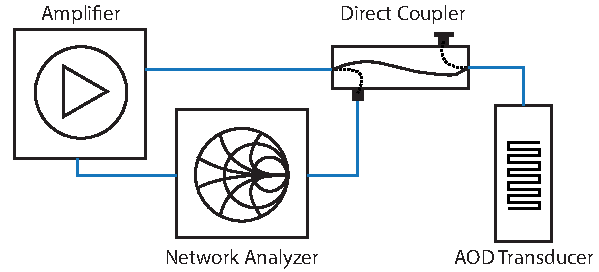
\includegraphics[width=.8\textwidth]{\figuredir{signal/setup-transducer.pdf}}
  \captionsetup{width=.8\textwidth}
  \caption{Experimental setup to measure the reflection at the acouso-optic
  transducer component. The network analyzer supplies an input signal to
  the amplifier. The output signal of the amplifier is connected through
  a direct-coupler with the acousto-optic element. The direct-coupler allows
  to safely measure input and output reflection.
  }\label{fig:signal_amplification_transducer_setup}
\end{figure}
The setup is depicted in \Cref{fig:signal_amplification_transducer_setup}.
The network analyzer on the left-hand side supplies an input signal to the
amplifier. The input signal changes linear in frequency. The output signal
of the amplifier is connected through a direct-coupler with the acousto-optic
element. The direct-coupler allows to measure input and output reflection.
\begin{figure}[ht]
  \centering
  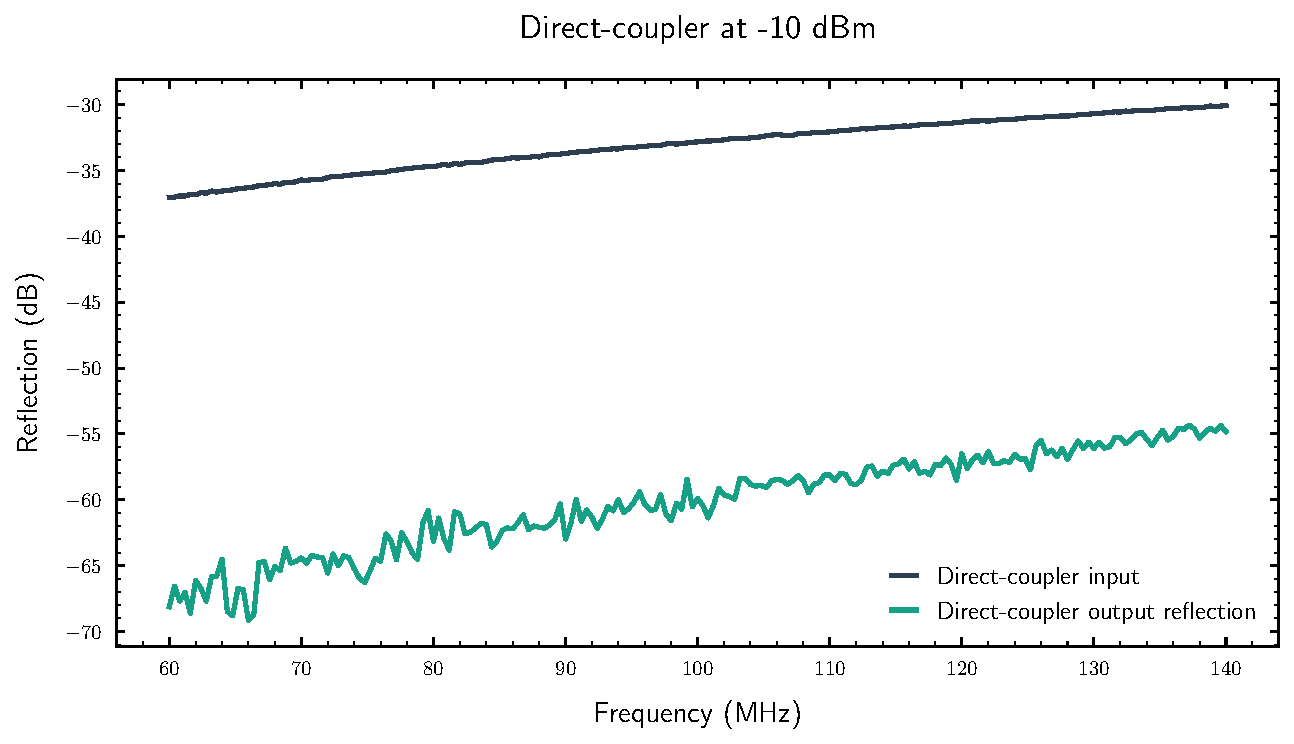
\includegraphics[width=\textwidth]{\figuredir{signal/reflection/coupler.pdf}}
  \captionsetup{width=.8\textwidth}
  \caption{Input power reflection when supplying the direct-coupler with
    \SI{-10}{\decibel\meter} input signal and reflection at the closed output
    of the direct-coupler while other ports are closed with \SI{50}{\ohm}.
  }\label{fig:signal_reflection_coupler}
\end{figure}
The direct-coupler is an apparatus comprising a coaxial input and output
port as well as a coaxial input reflection and output reflection port. It is
disignated to measure the reflection of a (possible) high power signal
without jeopardizing measurement equipement.
\begin{figure}[ht]
  \centering
  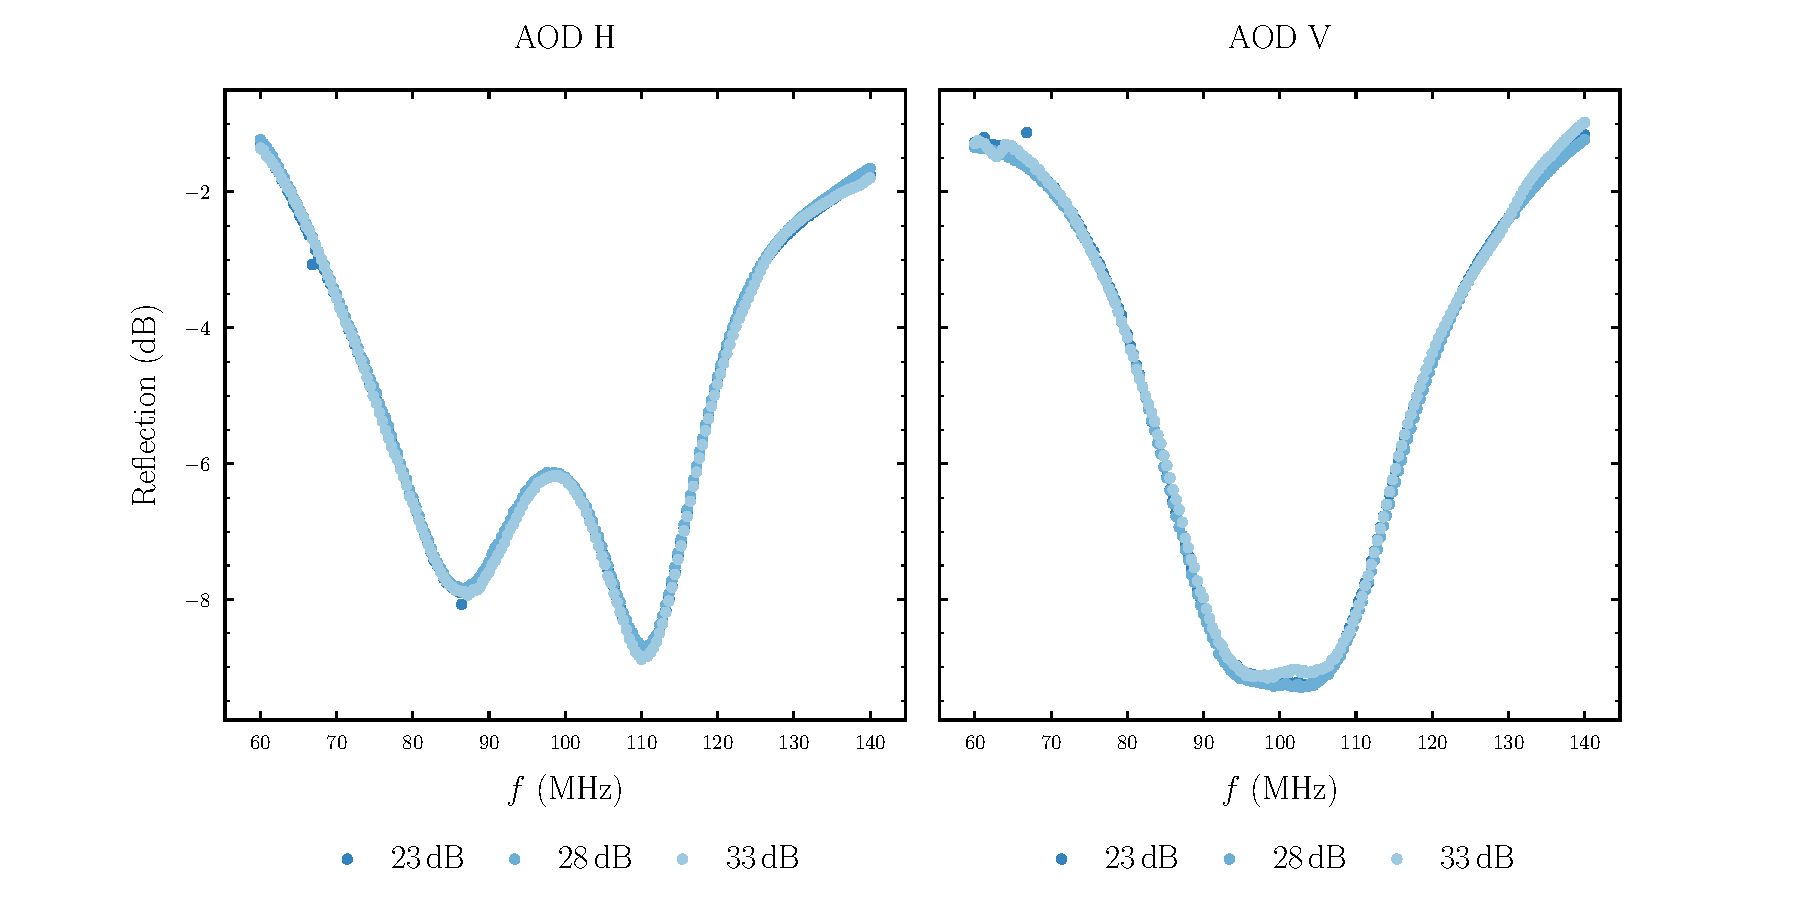
\includegraphics[width=\textwidth]{\figuredir{signal/reflection/coupled.pdf}}
  \captionsetup{width=.8\textwidth}
  \caption{Reflection at the direct-coupler output after amplification of the
  network analyzer input signal for different effective powers. We see that
the applied power does not effect the spectrum.
}\label{fig:signal_reflection_coupled}
\end{figure}
In \Cref{fig:signal_reflection_coupler} we see the reflection spectrum for
the case that we provide the network analyzer output signal to the input of
the direct-coupler and connect the reflection output of the direct-coupler
with the second network analyzer port while the remaining ports are under
\SI{50}{\ohm} closure.

We note that the reflection measured through the direct-coupler is lowered
by many orders of magnitude compared to the input signal but essentially of
the same shape. The noise in the reflection is very high because of the low
power supplied into the direct-coupler. We now use the direct-coupler to
measure the output reflection at the
\gls{aod} elements after the signal was amplified.

In \Cref{fig:signal_reflection_coupled} we see the effective reflection
spectrum for the distinct \gls{aod} elements. The effective reflection
spectrum is obtained when subtracting the input reflection from the output
reflection.

\subsubsection{Comparison}

In the previous part we saw that the reflection spectrum does not show any
power dependence, thus we should be able to compare the spectrum we obtained
directly with the amplified result.
\begin{figure}[ht]
  \centering
  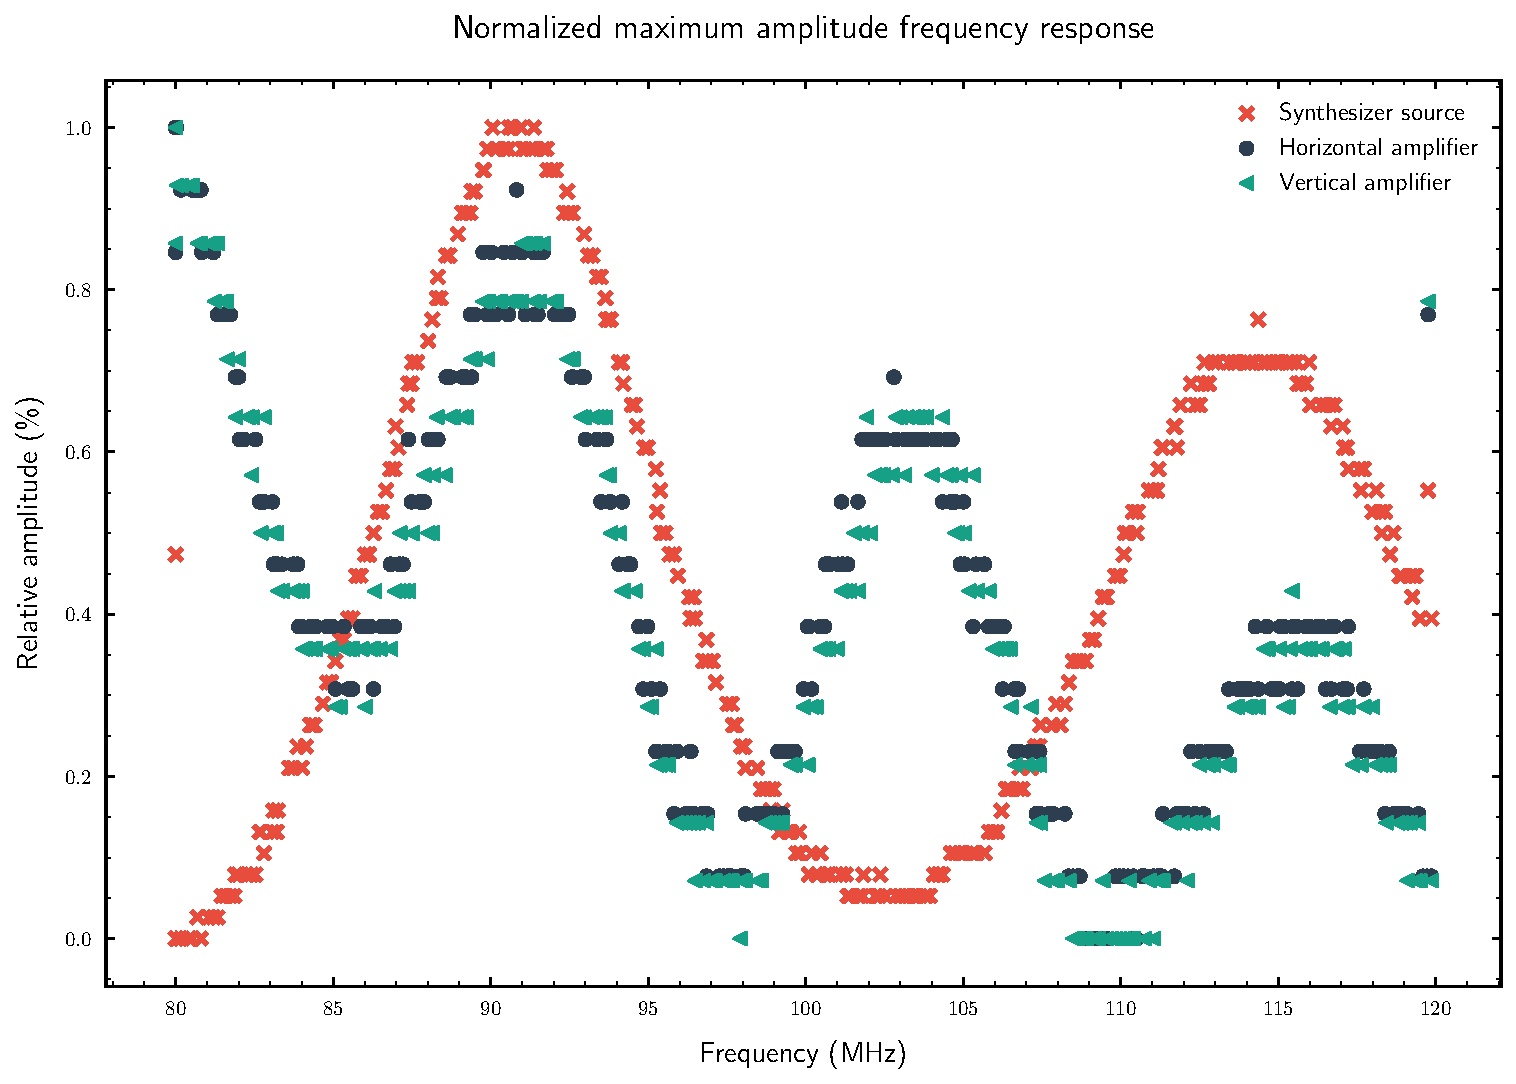
\includegraphics[width=\textwidth]{\figuredir{signal/reflection/comparison.pdf}}
  \captionsetup{width=.8\textwidth}
  \caption{Reflection from amplified input signal and direct signal as well as
    transmission from the amplifier spectrum.
  }\label{fig:signal_reflection_comparison}
\end{figure}
In \Cref{fig:signal_reflection_comparison} we can see how there is additional
reflection from the amplifier, nevertheless the global spectrum
characteristics stay in place.

\subsubsection{Summary}

Distinct \gls{aod} elements show different power transmission characteristics
independent of the applied power. Examination of the \gls{aod} elements in
details discloses different impedance matching circuits. Impedance matching
is used to reduce power reflection by providing a constant input resistance
of \SI{50}{\ohm} accross an ideally wide frequency range. Still the impedance
differs between the \gls{aod}s. We assume that the crystal properties
i.e.\ cut, purity are responsible for that, this is supported by the fact
that the impedance matching circuits differ between the \gls{aod} elements.

\chapter{Characterisation of the optical setup}

\textit{In the previous chapter we seeked for different aspects of the
\gls{rf} signal powering the \gls{aod} elements and found that the
electronic equipement provides an overall stable signal for the \gls{aod}.
In this chapter we want to examine the intensity characteristics subject
to frequency and amplitude parameters of the \gls{rf} signal. In the end
we will find that the intensity shows highly non-linear behaviour with
respect to the \gls{rf} signal parameters.}

\section{Intensity control}

In \cref{ch:experimental_setup} we stated that the laser intensity is
regulated by a control loop using an \gls{aom} in the power reduction setup.
Without the additional intensity regulation we would
observe various intensity drifts from the laser source throughout the
measurements as depicted in \Cref{fig:intensity_uncontrolled} where we can
observe short- and long-term oscillations over a large intensity range.
\begin{figure}[htb]
  \centering
  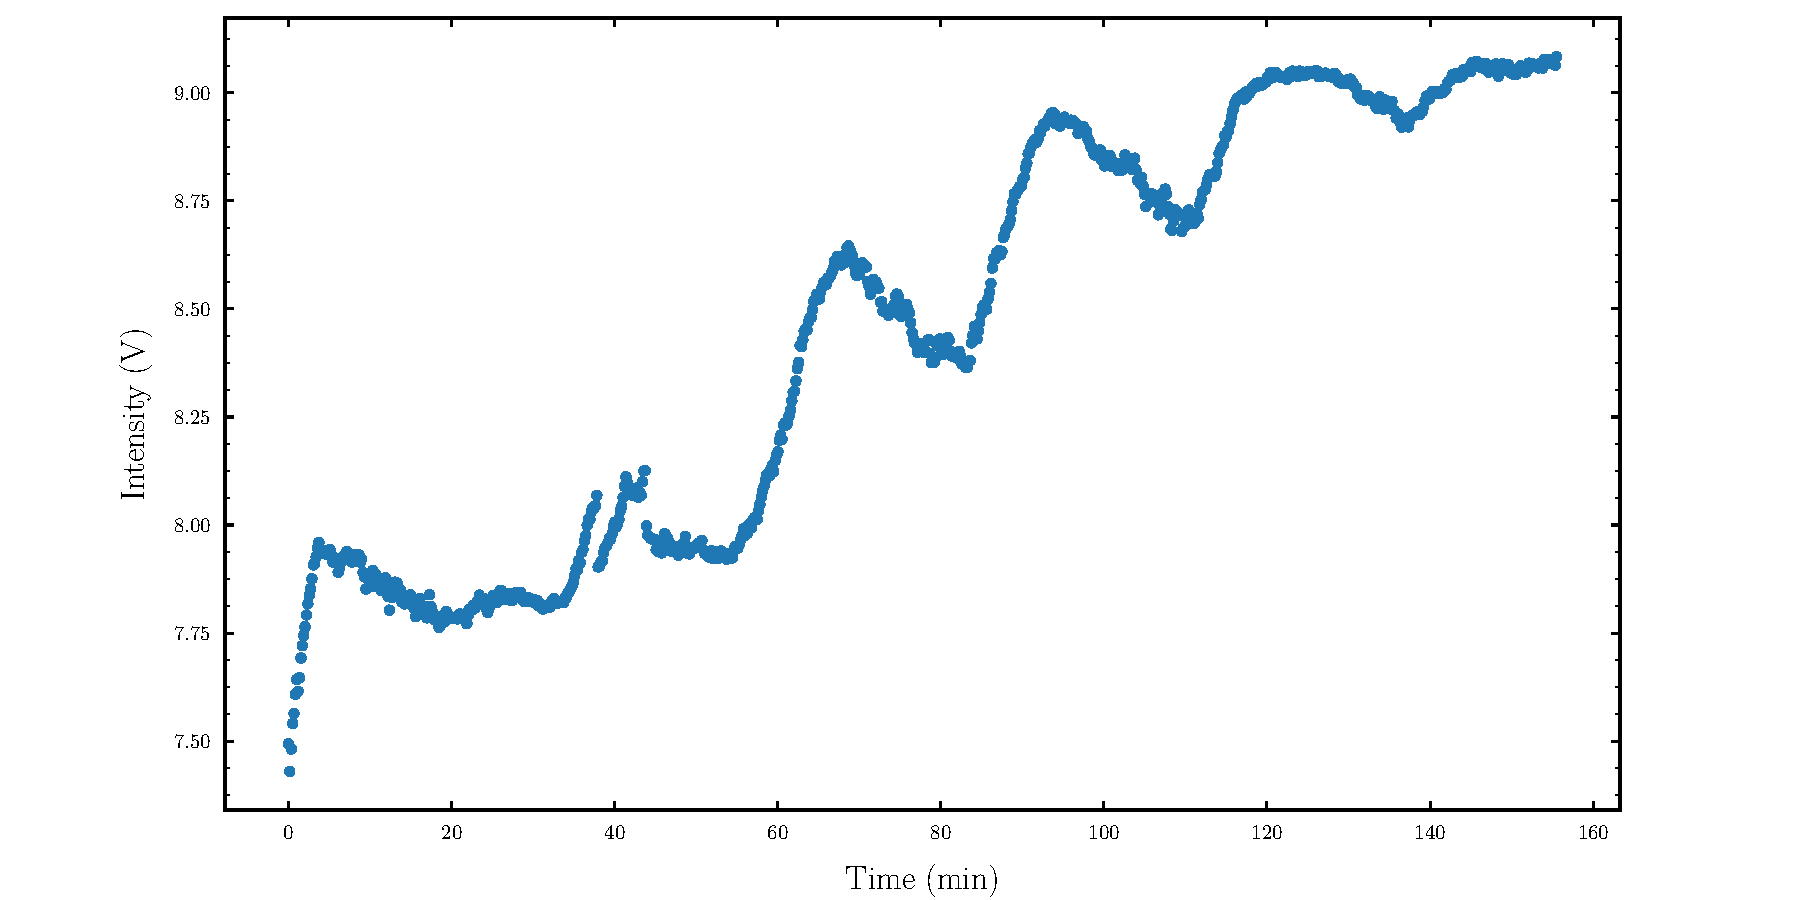
\includegraphics[width=\textwidth]
  {\figuredir{intensity/control/uncontrolled.pdf}}
  \captionsetup{width=.9\textwidth}
  \caption{Time evolution of the uncontrolled laser intensity.
  }\label{fig:intensity_uncontrolled}
\end{figure}
The setup used to record the intensity evolutions is disclosed in
\Cref{fig:intensity_control_setup}. It differs from the optical setup
described in \cref{ch:experimental_setup} by the absence of the \gls{aod}
and the relocation of Photodiode 2 at the end of the laser beam. The
photodiode gain of Photodiode 2 was lowered from \SI{70}{\decibel} to
\SI{50}{\decibel} because the lack of \gls{aod}s would otherwise cause the
photodiode to saturate.
\begin{figure}[htb]
  \centering
  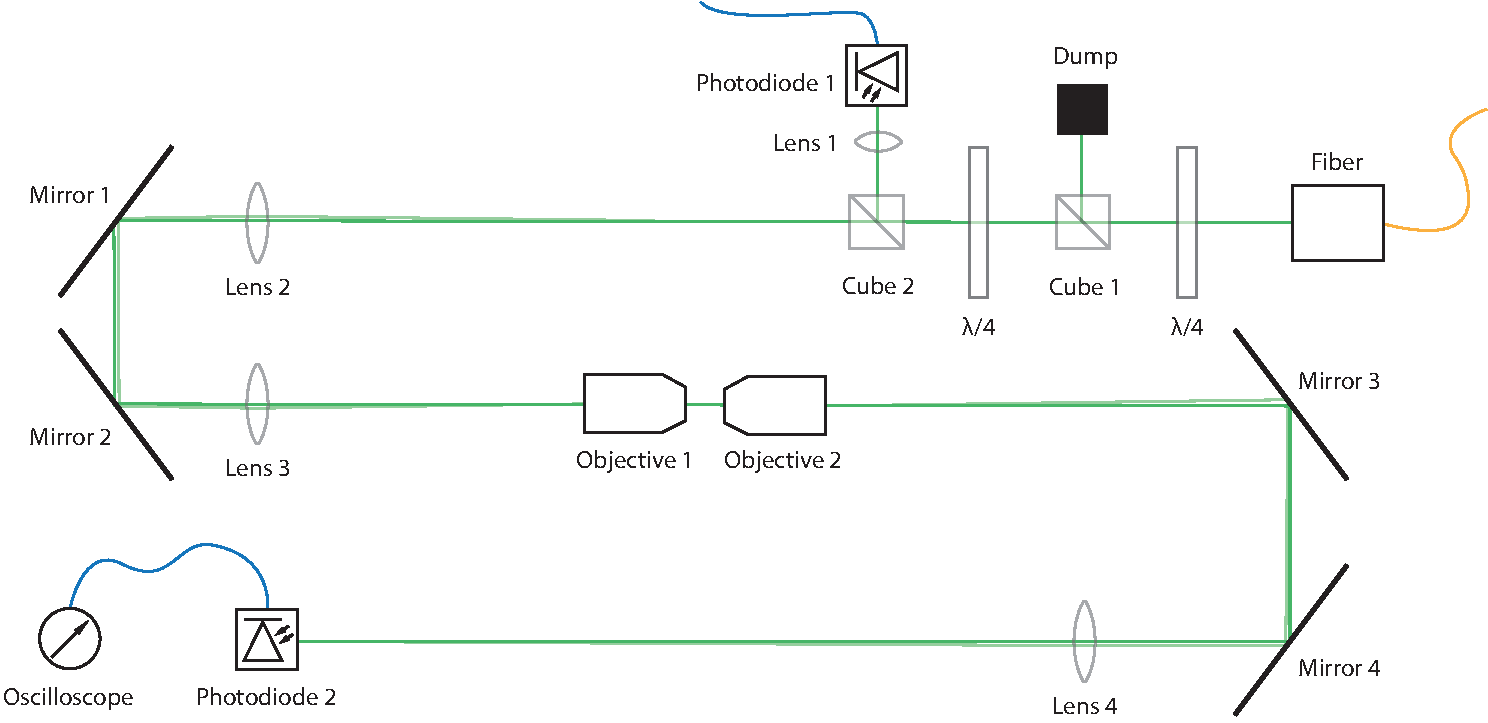
\includegraphics[width=.9\textwidth]{\mediadir{setup/intensity-control.pdf}}
  \captionsetup{width=.9\textwidth}
  \caption{Optical setup and intensity detection. The beam hits Photodiode 2
    which is connected to the oscilloscope.
  }\label{fig:intensity_control_setup}
\end{figure}
In order to to estimate the error contribution due to imperfect intensity
regulation, we will conduct a short- and a long-term measurement of the
controlled intensity. Technically a typical intensity measurement takes about
a fraction of a millisecond, yet we can decide on different intervals between
the measurements in order to separate local from global trends like the ones
noted in the uncontrolled meausrement. \Cref{tab:intensity_control_times}
summarizes the different time scales for the conducted short- and long-term
measurement of the intensity control.
\begin{table}[htb]
  \centering
  \begin{tabular}{cccc}
    \toprule
    & Short & Long & Typical \\
    \midrule
    Interval &
    \SI{10}{\second} &
    \SI{120}{\second} &
    \SI{3}{\second} \\
    Duration &
    \SI{1}{\hour} &
    \SI{16}{\hour} &
    \SI{<2}{\hour} \\
    \bottomrule
  \end{tabular}
  \captionsetup{width=.9\textwidth}
  \caption{Interval and duration times of the short- and long-term measurement
    as well as a typical sweep measurement.
  }\label{tab:intensity_control_times}
\end{table}
The voltage time series for both intensity control measurements are presented
in \Cref{fig:intensity_control}. The outlier at about 22:45 h was caused by
accidently interfering with the setup during measurement. Beside of that
incident the long-term intensity seems stable. On a smaller timescale we see
that the intensity evolution performs periodic oscillations.
\begin{table}[htb]
  \centering
  \begin{tabular}{lcccc}
    \toprule
    Measure & Uncontrolled & Long & Short & Typical \\
    \midrule
    Mean $\mu$ &
    \SI{8.45}{\volt} &
    \SI{6.79}{\volt} &
    \SI{6.79}{\volt} &
    \SI{1.95}{\volt} \\
    Minimum &
    \SI{7.43}{\volt} &
    \SI{4.88}{\volt} &
    \SI{6.77}{\volt} &
    \SI{0.00}{\volt} \\
    Maximum &
    \SI{6.82}{\volt} &
    \SI{6.86}{\volt} &
    \SI{6.82}{\volt} &
    \SI{9.08}{\volt} \\
    Standard Deviation $\sigma$ &
    \SI{0.49}{\volt} &
    \SI{0.09}{\volt} &
    \SI{0.01}{\volt} &
    \SI{0.54}{\volt} \\
    Relative Standard Deviation $\sigma/\mu$ &
    \SI{5.75}{\percent} &
    \SI{1.35}{\percent} &
    \SI{0.19}{\percent} &
    \SI{27.69}{\percent} \\
    \bottomrule
  \end{tabular}
  \captionsetup{width=.9\textwidth}
  \caption{Descriptive statistics of uncontrolled and controlled short- and
    long-term intensity evolutions as well as a typical intensity measurement
    with \gls{aod}s for comparison.
  }\label{tab:intensity_control_statistics}
\end{table}
Overall we can confirm that the intensity control loop successfully holds the
intensity mean, though with small oscillations. In order to estimate the
relevance for these small oscillations of the controlled intensity for later
measurements, we selected an measurement of the intensity transmission
response of the \gls{aod} subject to constant frequency increments for
comparison. \Cref{tab:intensity_control_statistics} presents the statistics of
said intensity measurements.
\begin{figure}[htb]
  \centering
  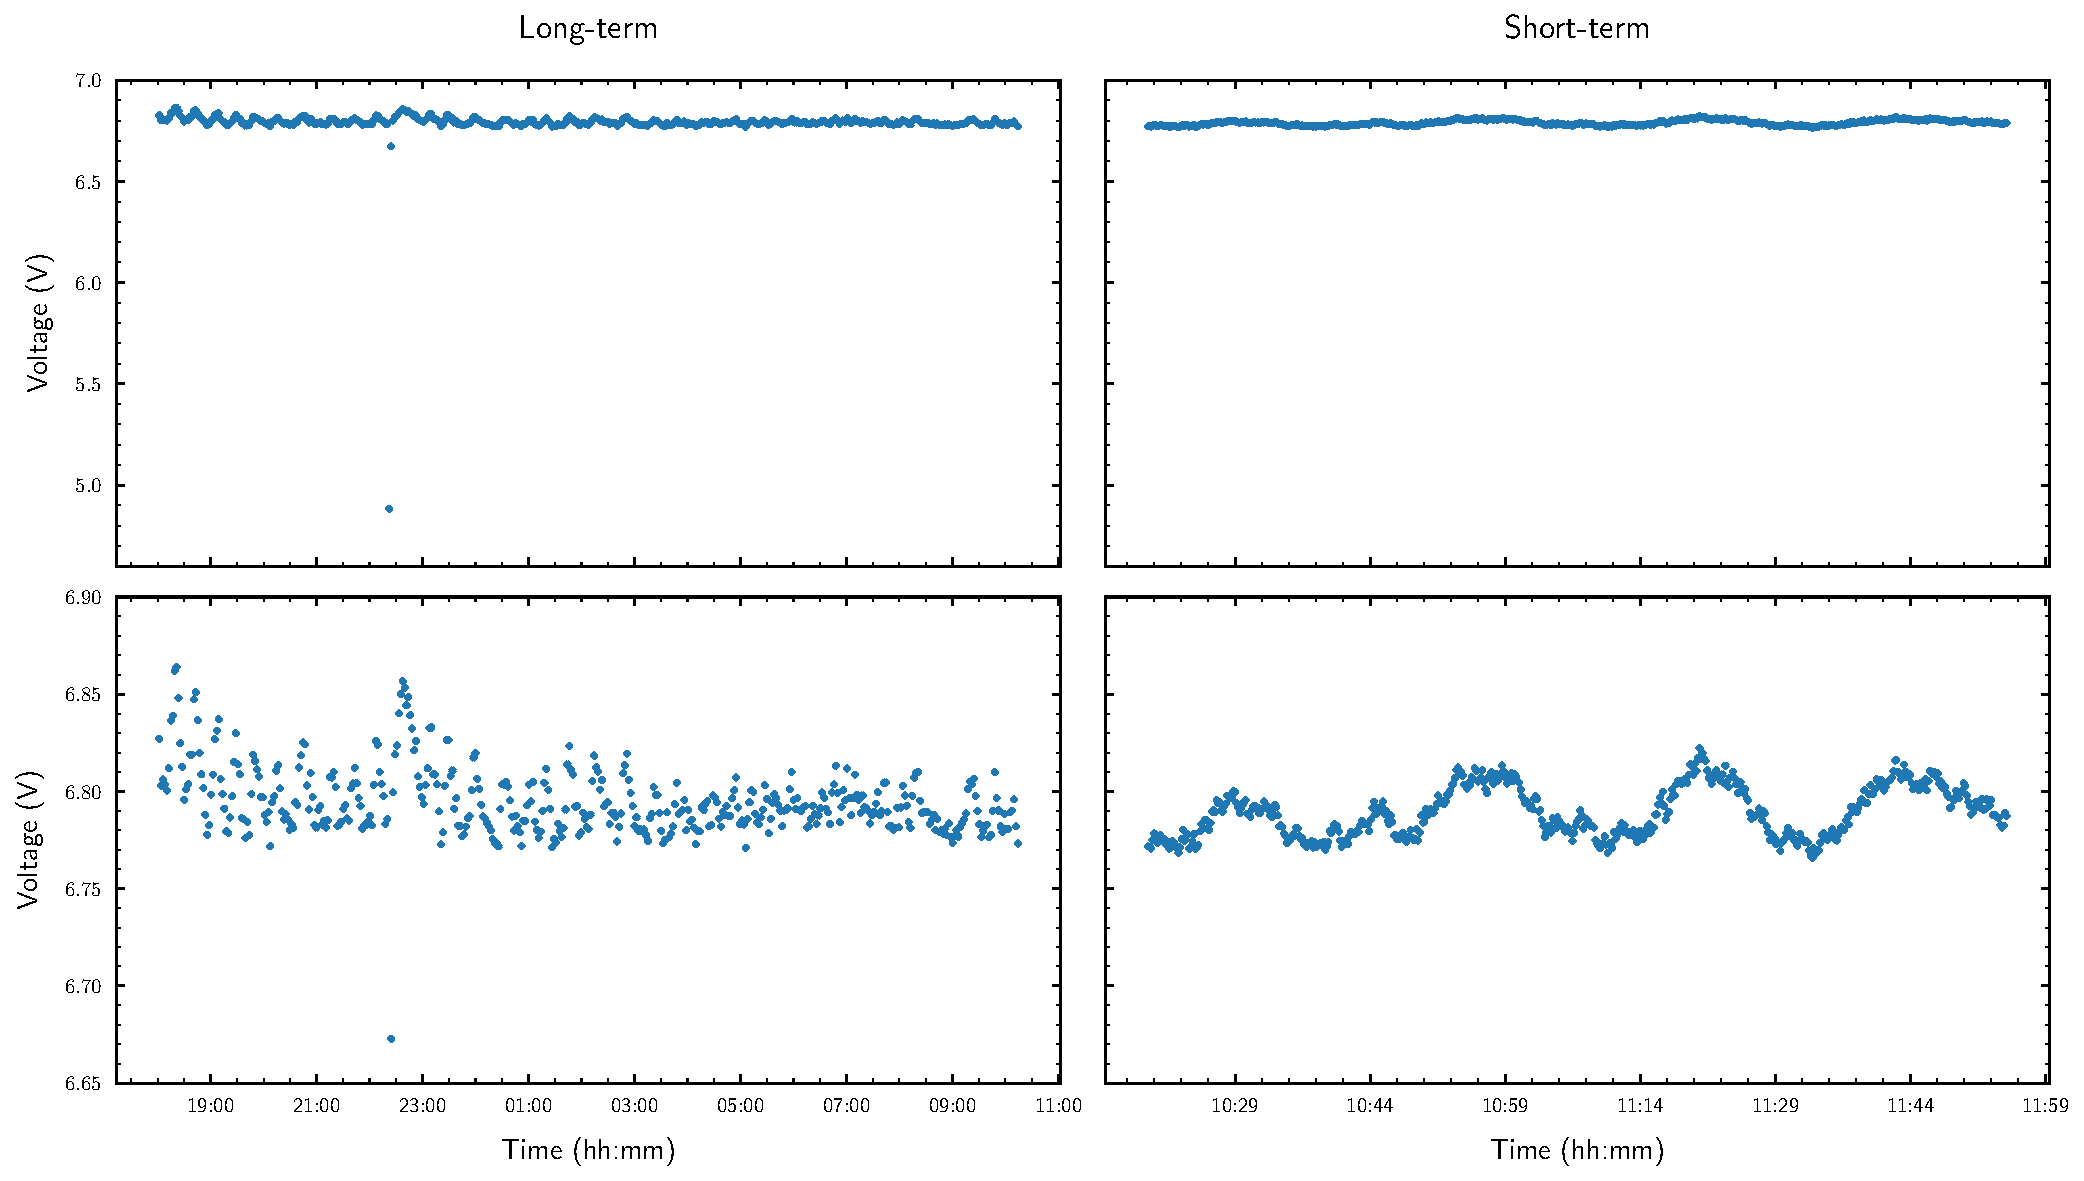
\includegraphics[width=\textwidth]{\figuredir{intensity/control/long-short.pdf}}
  \captionsetup{width=.9\textwidth}
  \caption{Long- and short-term measurement of the controlled intensity at
    different voltage scales.
  }\label{fig:intensity_control}
\end{figure}
We should note that not all of the statistical measurements are directly
comparable because of the \SI{20}{\decibel} higher photodiode gain used in
the typical measurement with \gls{aod}s. Nevertheless we can directly compare
the uncontrolled and the controlled short- and long-term measurements
directly. As we divide by the mean $\mu$, the relative standard deviation
$\sigma/\mu$ is a scale invariant statistical measure and thereby comparable
through measurements conducted with different photodiode gain setting.
Comparing the relative standard deviation yields that the intensity drifts
are small on a short time scale compared to intensity variations in a typcial
measurement. In contrast the uncontrolled intensity --- also conducted on
a short-term time scale --- contributes a significant error. In order to
compare the intensity deviations further we calculate the \gls{rmd} via
\begin{equation}
  I_\text{rmd}
  =
  \frac{I-\overline{I}}{\overline{I}}
  \label{eq:relative_mean_deviation}
\end{equation}
where $\overline{I}$ denotes the intensity mean. In
\Cref{fig:intensity_control_rmd} the \gls{rmd} of the controlled and
uncontrolled as the controlled measurements are presented as boxplots.
\begin{figure}[htb]
  \centering
  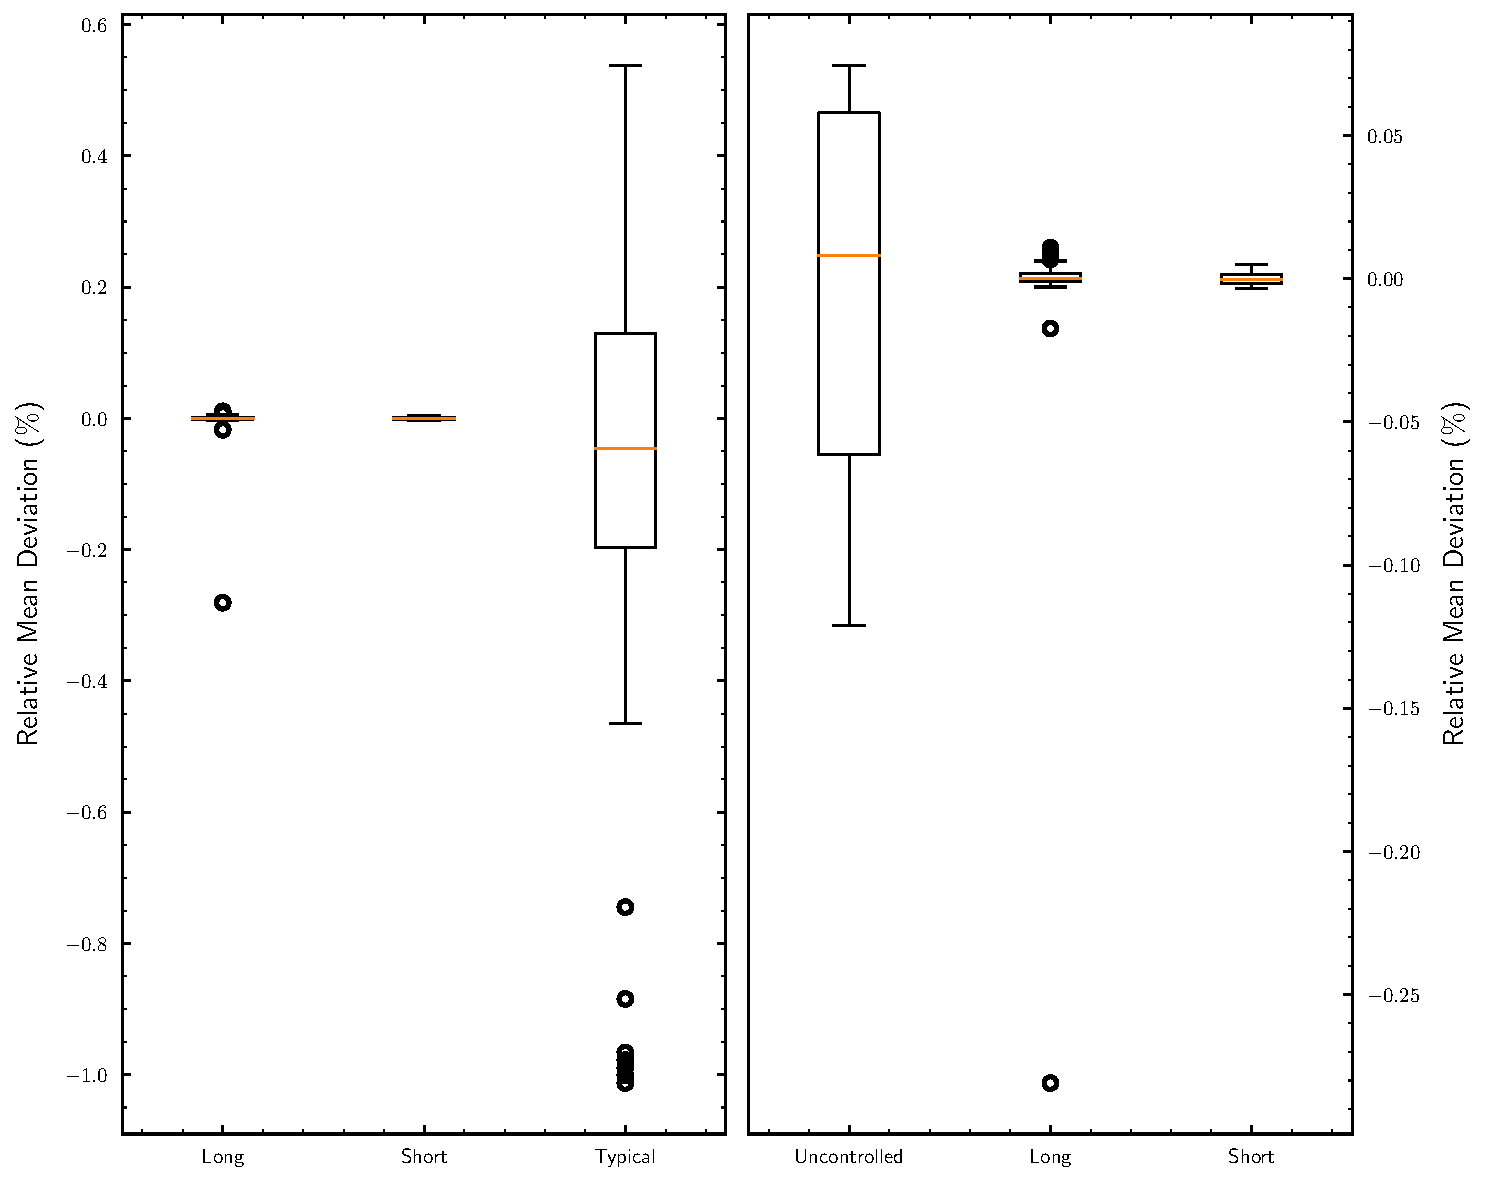
\includegraphics[width=\textwidth]
  {\figuredir{intensity/control/relative-mean-deviation.pdf}}
  \captionsetup{width=.9\textwidth}
  \caption{Relative mean deviation of uncontrolled and controlled long- and
    short-term measurement as well as typical controlled intensity measurement.
  }\label{fig:intensity_control_rmd}
\end{figure}
Boxplots are heavily based on the concept of \gls{iqr}. The \gls{iqr} is a
scale invariant measure of statistical dispersion and is defined as the
inverse of the \gls{cdf}. The start and end of the boxes inside a boxplot
denote the lower (first) quantile $Q_1$ and the upper (third) quantile $Q_3$
of the \gls{iqr}. Expressed through the \gls{cdf} these read
\begin{align}
  Q_1=\text{CDF}^{-1}{\left(\frac{1}{4}\right)} &&
  Q_3=\text{CDF}^{-1}{\left(\frac{3}{4}\right)}.
\end{align}
Alternatively one can define $Q_1$ as the median of the $n$ smallest entries
and $Q_3$ as the median of the $n$ largest entries where the total dataset
consists out of $2n$ entries for the even and $2n+1$ entries for the odd case.
The whiskers below and atop of the boxes are at $Q_1\pm1.5IQR$. Values outside
this range are usually considered outliers and marked as circles. The median
is denoted with an orange line. The left boxplot confirms that the
oscillations of the controlled intensity are negligible for typical intensity
measurements. Further the right boxplot confirms that the intensity control
oscillations cover a much smaller range as the uncontrolled oscillations.

\section{Beam profile}

Perpendicular to the error introduced by the imperfect intensity control,
errors can originate from unideal optical alignment. One way to assess the
quality of our alignment is to evaluate the spatial profile of the laser beam
as registered with the \gls{ccd} camera.
\begin{figure}[htb!]
  \centering
  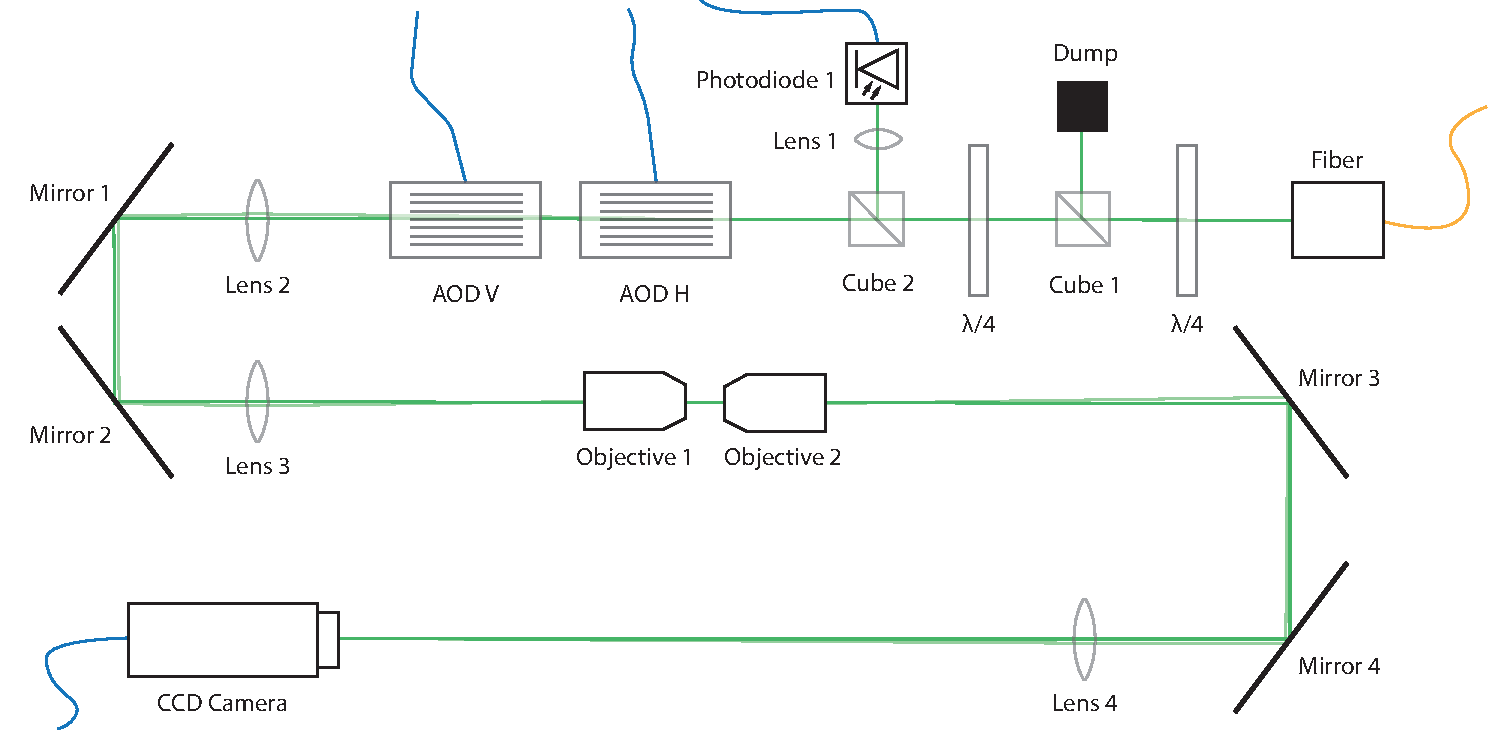
\includegraphics[width=\textwidth]{\mediadir{setup/intensity-profile.pdf}}
  \captionsetup{width=.9\textwidth}
  \caption{The beam is focused onto the \gls{ccd} sensor of the camera.
  }\label{fig:intensity_profile_setup}
\end{figure}
In \Cref{fig:intensity_profile_setup} we present the setup used to measure
the spatial beam profile. In comparison to the previous setup we replaced
Photodiode 2 with a \gls{ccd} camera. The \gls{aod}s are configured at a
center frequency of \SI{100}{\mega\hertz}. The distance between Lens 4 and
the \gls{ccd} sensor is chosen such that the laser beam is focused onto the
\gls{ccd} sensor of the camera.
\begin{figure}[htb]
  \centering
  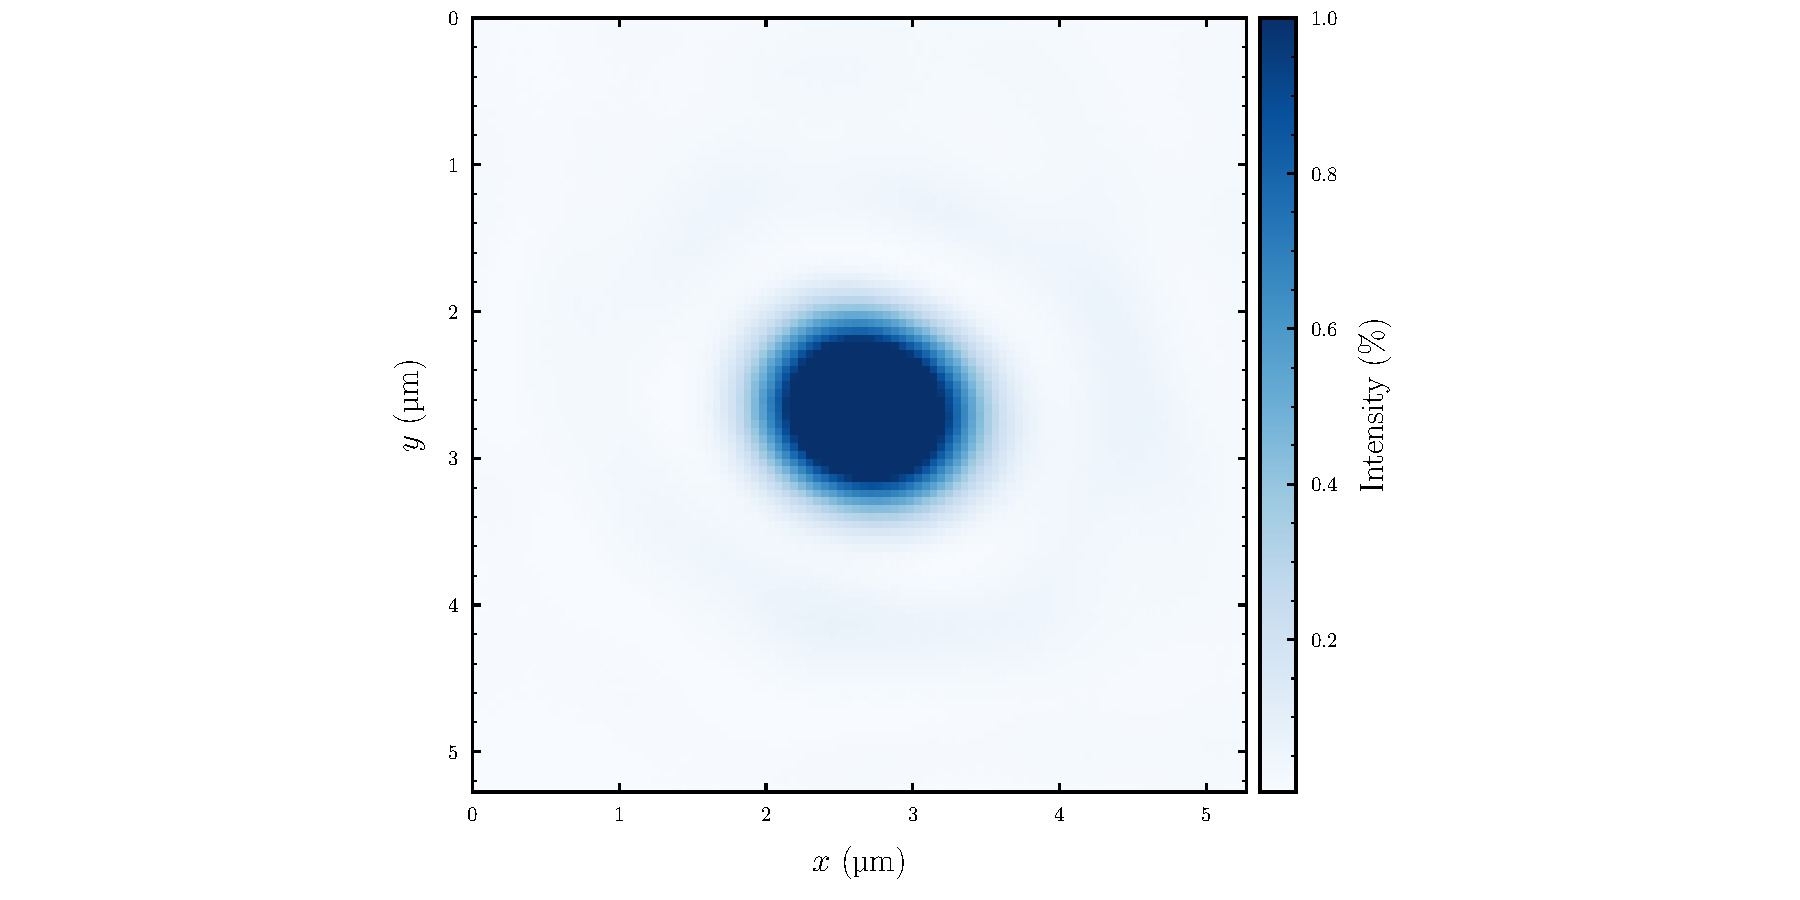
\includegraphics[width=.6\textwidth]
  {\figuredir{intensity/profile/image.pdf}}
  \caption{Image of the focused laser beam measured with the \gls{ccd} camera.
  }\label{fig:intensity_spatial_image}
\end{figure}
\Cref{fig:intensity_spatial_image} shows an enlarged image patch of the
complete image capture taken with the \gls{ccd} camera. We can see a strong
illuminated circular spot in the center of the image with an area of about
\SI{2.5}{\milli\meter}. The intensity inside the spot seems homogeneous,
however this is caused by a saturation of the pixels in this area. We could
reduce the intensity or apply an optical filter to the camera to resolve the
intensity gradient inside the spot, but only at the cost of the intensity
distribution around the spot. Around the circular spot we can see a
diffraction ring. The diffraction ring is well described
in~\cite{Hertlein2017} and originates from the finite aperture of the
objectives.
\begin{figure}[htb]
  \centering
  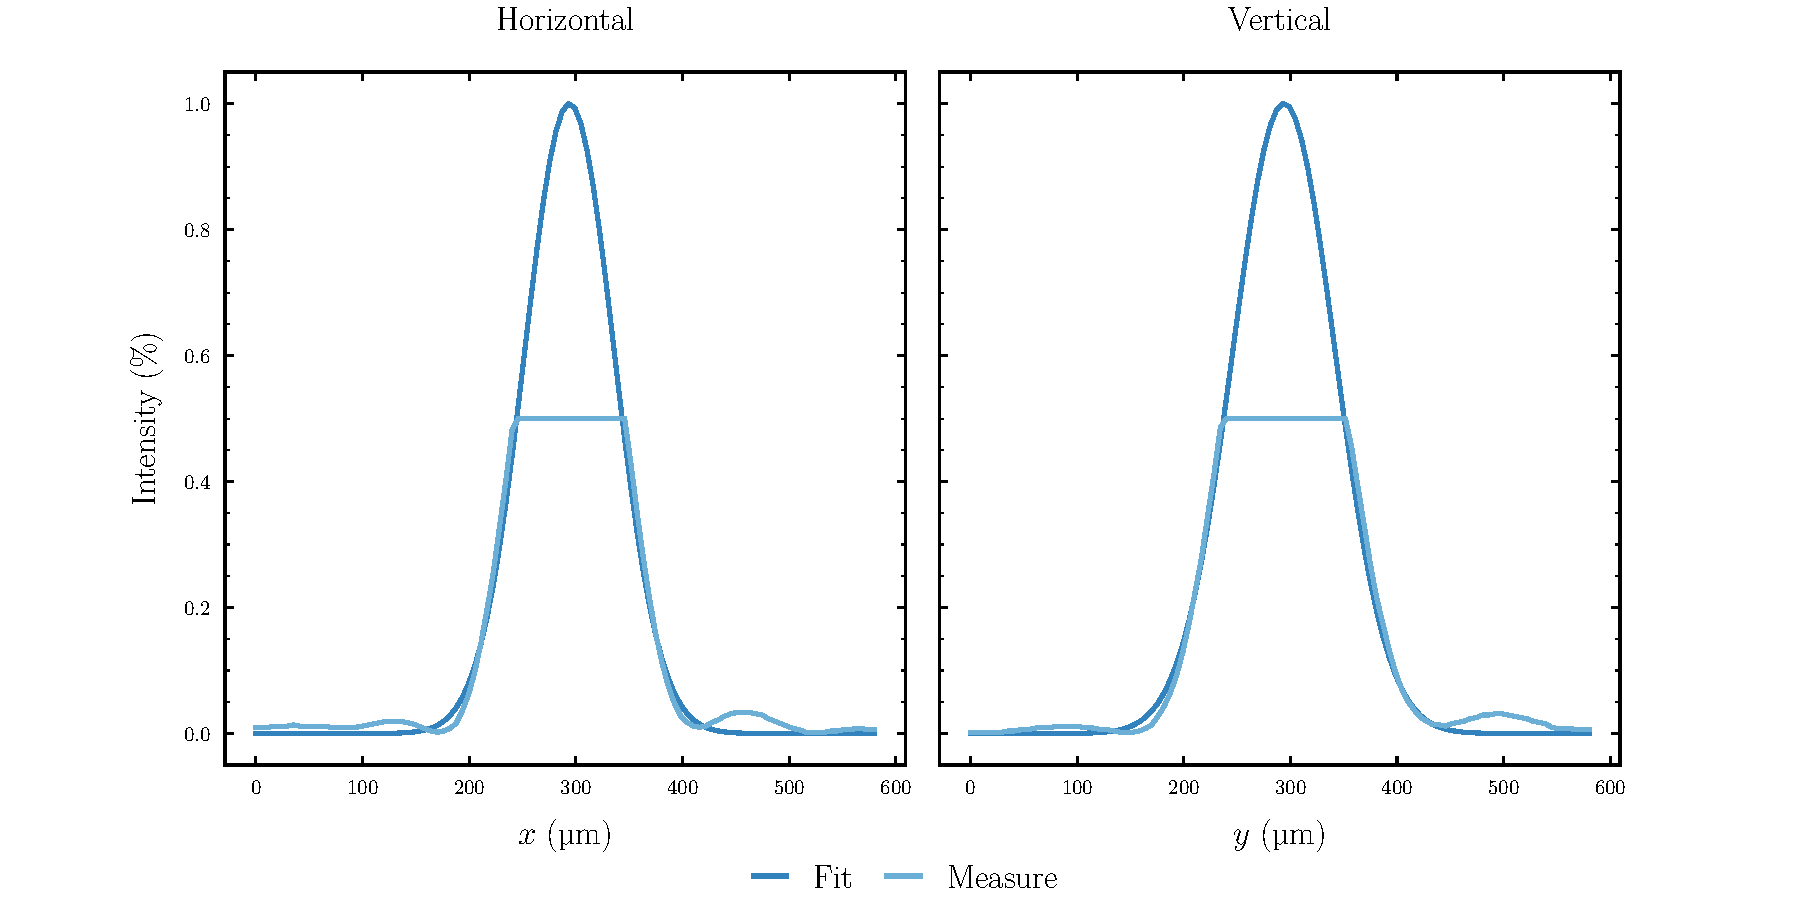
\includegraphics[width=.9\textwidth]{\figuredir{intensity/profile/profile.pdf}}
  \captionsetup{width=.9\textwidth}
  \caption{One dimensional perpendicular cut of the two dimensional intensity
    distribution from the two dimensional beam profile in
    \Cref{fig:intensity_spatial_image} with fitted gaussian curve.
  }\label{fig:intensity_spatial_profile}
\end{figure}
For better comparison of the radial symmetry we performed two perpendicular
cuts and visualized the one dimensional spatial beam distribution in
\Cref{fig:intensity_spatial_profile}.
In \Cref{fig:intensity_spatial_profile} we can clearly observe the effects of
saturation around the center and how we would expect the intensity to be
if we could experimentally resolve it in the Gaussian fit. In contrast to the
ideal Gaussian profile we again observe contributions to the Airy disc around
the otherwise Gaussian profile causes by the finite aperture. Further we can
now clearly observe assymmetry from the intensity contributions around the
Gaussian which means that our alignment is not perfect.

We can confirm the results reported in~\cite{Hertlein2017} that the spatial
beam profile equals a two dimensional Gaussian combined with a Airy disks
caused from the finite aperture of the objectives. Further we observe
slight assymmetries in the diffraction ring suggesting inperfect alignment.
Though asymetries in the spatial beam profile are present, we do not see any
further complications as the intensity measurements with the photodiode will
cover the complete beam profile.

\section{Difference between individual acousto-optic deflectors}

Our optical setup uses a single two dimensional \gls{aod} that comprises two
\gls{aod} elements perpendicular to each other. At first we want to examine the
behaviour of the individual \gls{aod} elements to each other. In particular we
are interested if and how the elements differ.
\begin{figure}[htb]
  \centering
  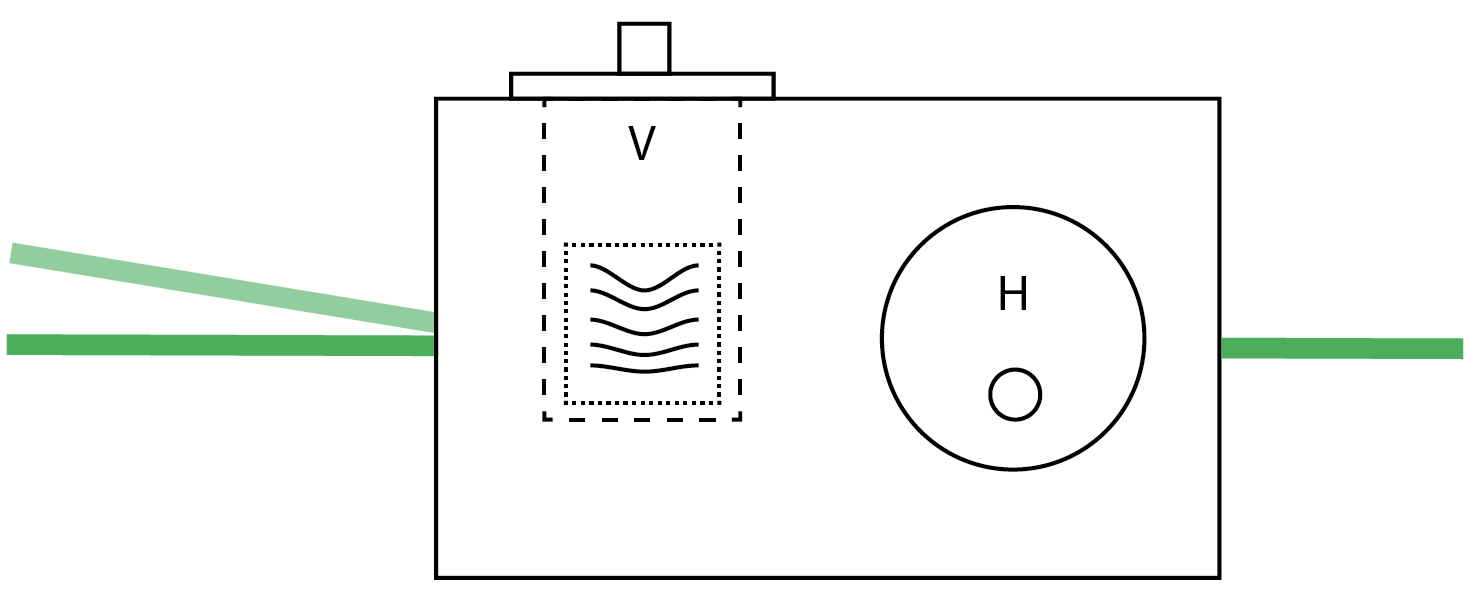
\includegraphics[width=\textwidth]{\mediadir{setup/aod-socket.png}}
  \captionsetup{width=.9\textwidth}
  \caption{Drawing of the used 2D \gls{aod}.
  }\label{fig:aod_socket}
\end{figure}
A schematic drawing of the \gls{aod} is depicted in \Cref{fig:aod_socket}. We
see the two \gls{aod} elements in the respective horizontal and vertical slot.
The internals of the vertical \gls{aod} (left-hand side) are illustrated. The
element itself spans through the casing (dashed line) while the acousto-optic
crystal (dotted line) is glued onto the element. The laser beam (green) passes
through the acousto-optic crystal. In the following we will refer to the
horizontal \gls{aod} element as the \gls{aod} element anticipated for the
horizontal slot and accordingly to the vertical \gls{aod} element as the
\gls{aod} element intended for the vertical \gls{aod} socket.

\subsection{Individual acousto-optic deflectors}

For the following experiment we will only leave one \gls{aod} element mounted
in the casing depicted in \Cref{fig:aod_socket}. The other slot will be empty.
Then we will exchange socket positions for each respective \gls{aod} element
and measure the beam intensity subject to the linear frequency sweep from
\SI{80}{\mega\hertz} to \SI{120}{\mega\hertz} over a duration of
\SI{260}{\milli\second} and the configured \gls{dds} amplitude. As \gls{rf}
signal source the amplifier and \gls{dds} combination intended for the
horizontal \gls{aod} element was used to avoid influences of the amplification
offset between the two amplifiers.
\begin{figure}[htb]
  \centering
  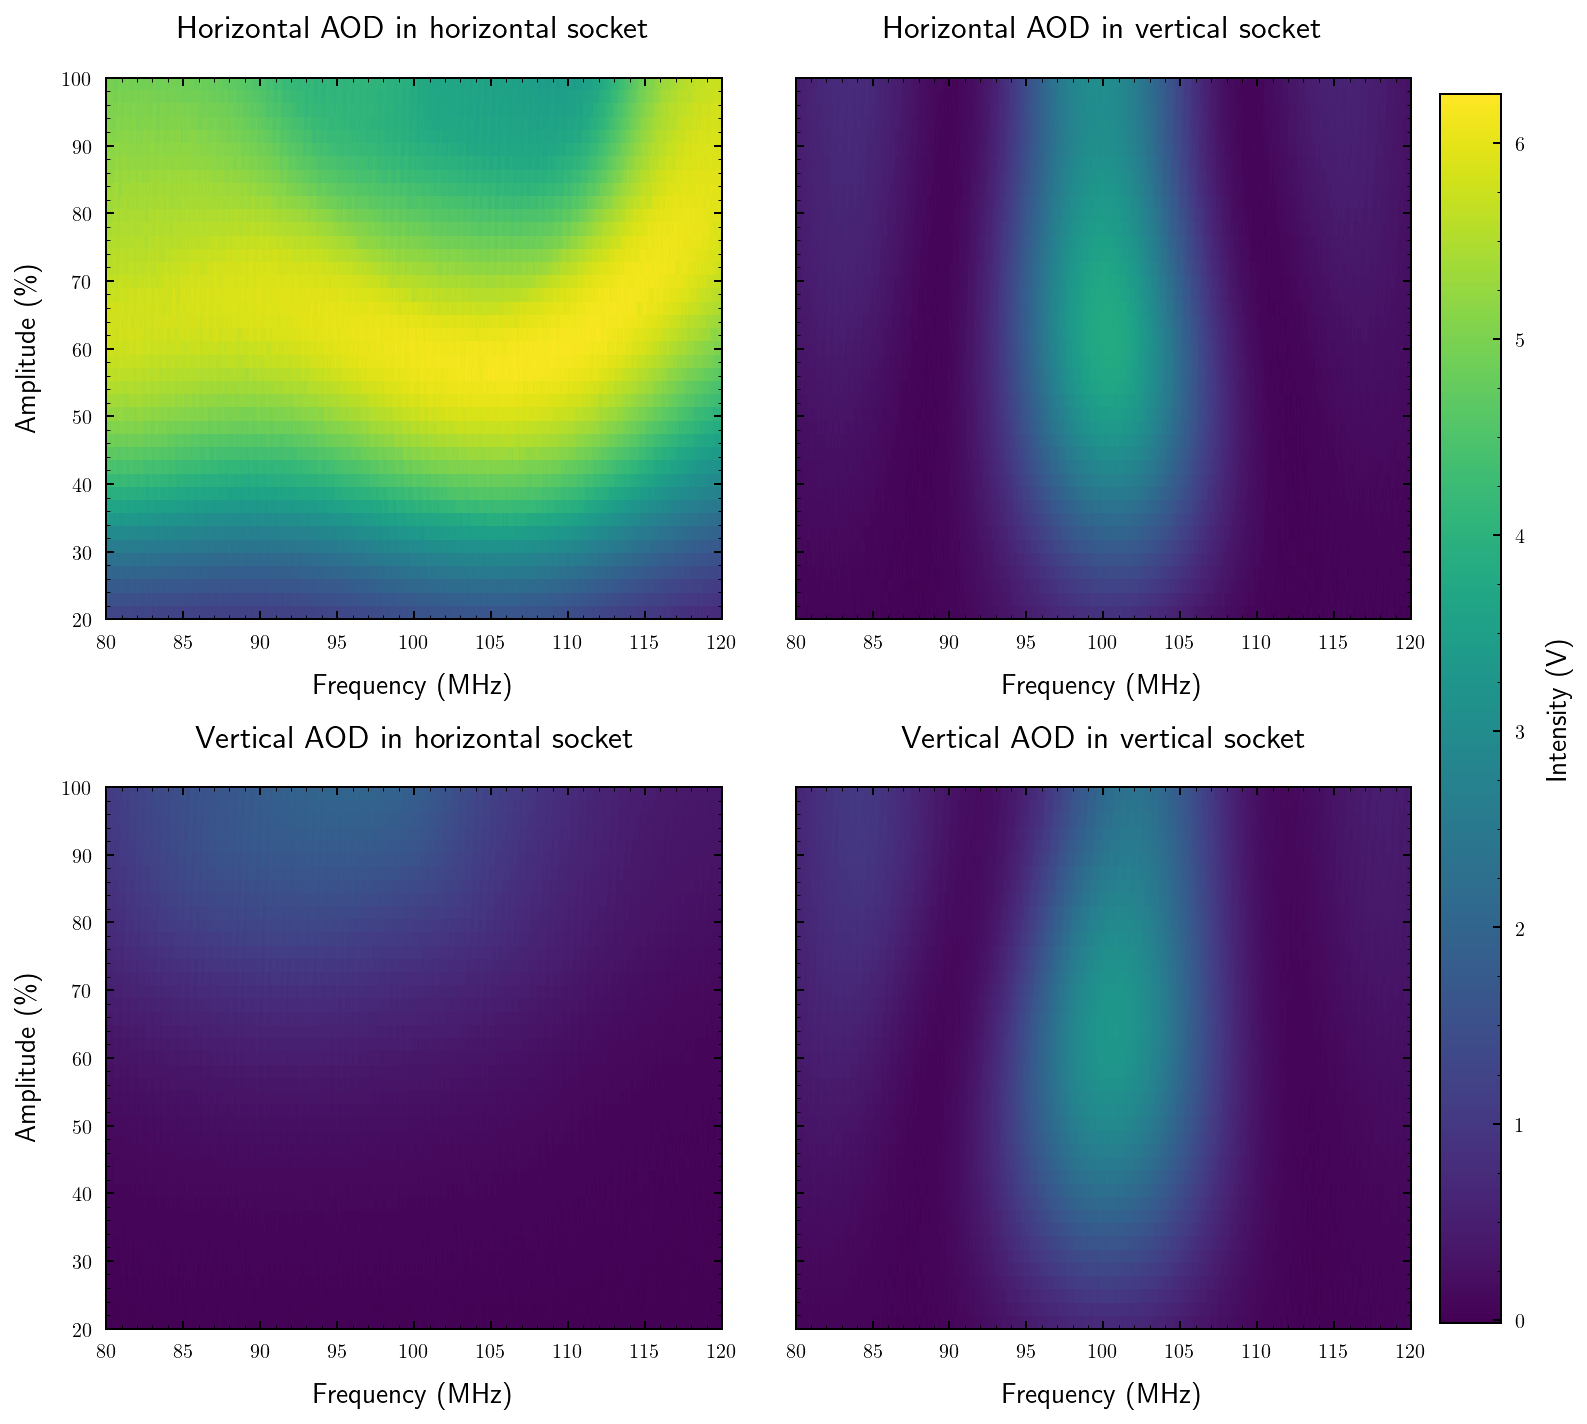
\includegraphics[width=\textwidth]
  {\figuredir{intensity/distribution/unpaired-amplitude.png}}
  \captionsetup{width=.8\textwidth}
  \caption{Intensity distribution over linear frequency sweep at different
    configured \gls{dds} amplitudes for different individual \gls{aod}
    configurations.
  }\label{fig:intensity_distribution_unpaired}
\end{figure}
The results for the four configurations (horizontal element in horizontal
slot, horizontal element in vertical slot, vertical element in horizontal
slot and vertical element in vertical slot) are visualized as heatmaps in
\Cref{fig:intensity_distribution_unpaired}. The color values are normalized in
between the different heatmaps and can be related to the measured voltage from
the photodiode via the colorbar on the right-hand side. Oddly enough we
observe that both \gls{aod}s differ strongly in their respective intensity
transmission behaviour depending on their slot position. Furthermore we
observe that the intensity transmission is much higher in the case of the
horizontal \gls{aod} element mounted to the intended horizontal slot compared
to all other configurations. In addition we can see that the intensity map
measured with the horizontal \gls{aod} displays a jump. The highest intensity
transmission is obtained for relative amplitudes configured between
\SI{60}{\percent} and \SI{90}{\percent} with large dependence on the
frequency. Another interesting observation is that the intensity transmission
seems very similar for the horizontal element in the vertical slot and the
vertical element in the vertical slot whose map also seems more symmetric with
respect to the frequency axis. In fact for these configurations the amplitude
dependence seems to be essentially independent of the frequency dependence.
We assume that the individual elements are designed for different
polarisation angles. In order to prove this hypothesis we added a tunable
$\lambda/2$ retarder plate after Cube 2. Tuning the $\lambda/2$ retarder
before Cube 2 would change the intensity fraction that gets redirected into
the beam dump as Cube 2 is a beam splitter sensible to polarisation.
\begin{figure}[htb]
  \centering
  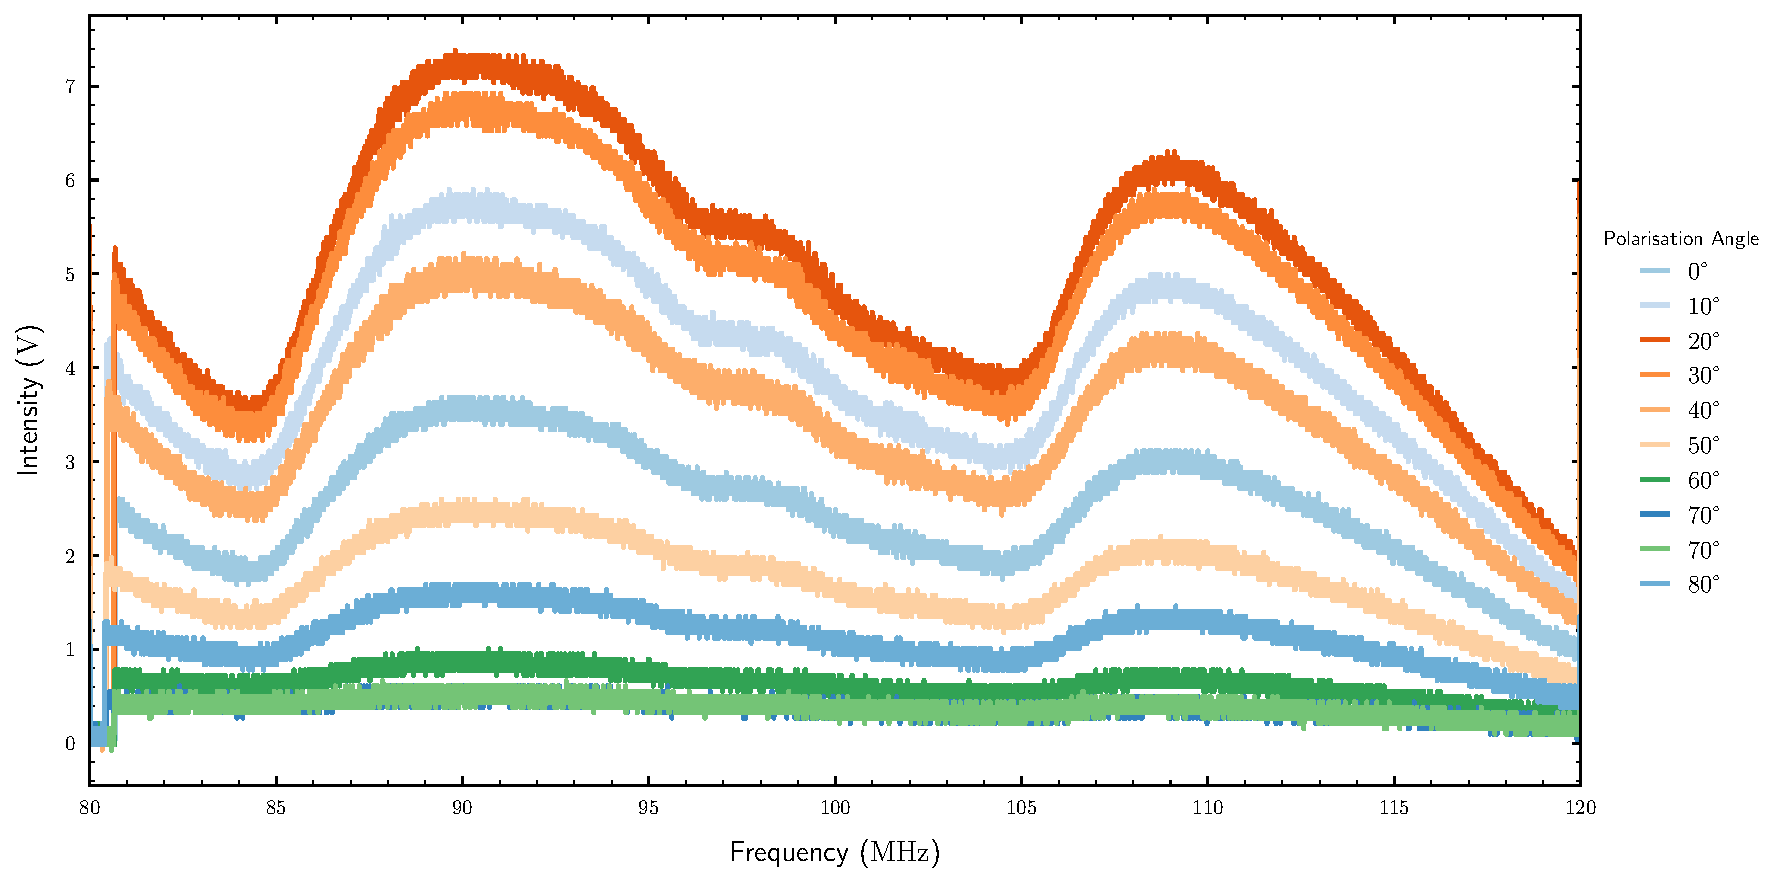
\includegraphics[width=\textwidth]
  {\figuredir{intensity/distribution/polarisation-horizontal.pdf}}
  \captionsetup{width=.8\textwidth}
  \caption{Intensity transmission of the \gls{h} \gls{aod} in the \gls{h} slot
    at maximum output amplitude for different polarisation angles.
  }\label{fig:intensity_polarisation_h}
\end{figure}
In \Cref{fig:intensity_polarisation_h} the intensity transmission of the
\gls{h} \gls{aod} in the \gls{h} slot at maximum output amplitude is presented
for different polarisation angles. The polarisation angles are the remainders
of the angles read of from the retarder plate mount divided by \ang{90}. The
reason behind this step is that a rotation of a retarder plate by $\phi$
effectively changes the polarisation angle by $2\phi$. Further the
polarisation domain is limited to $\left[0,\ang{90}\right]$.
\begin{figure}[htb]
  \centering
  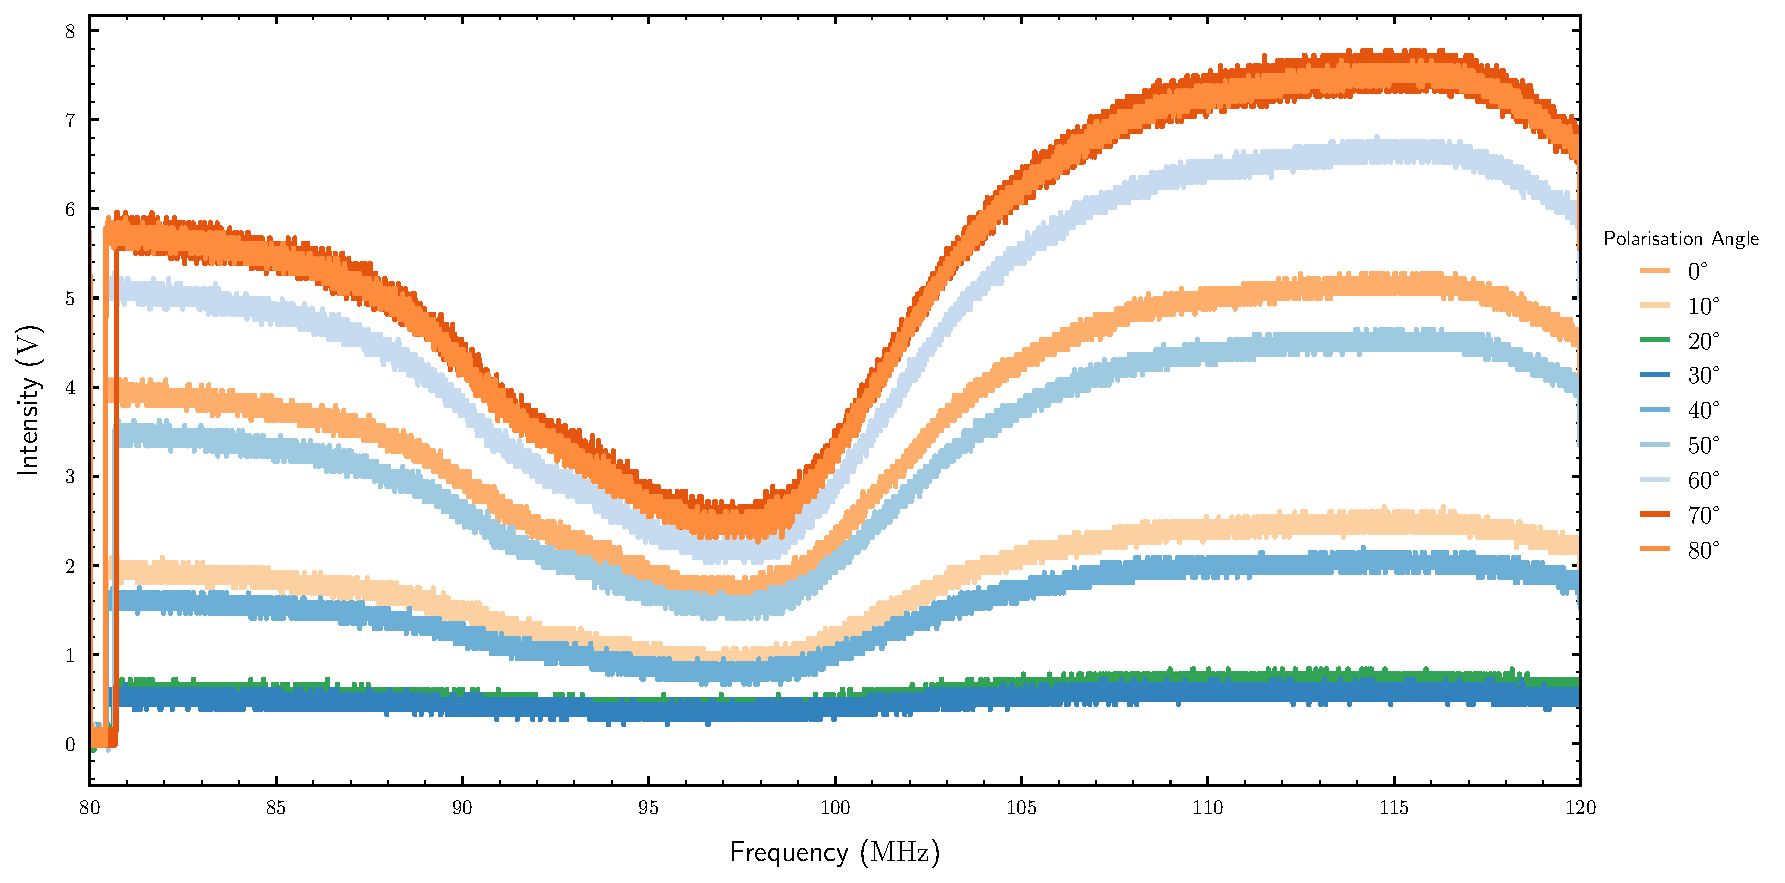
\includegraphics[width=\textwidth]
  {\figuredir{intensity/distribution/polarisation-vertical.pdf}}
  \captionsetup{width=.8\textwidth}
  \caption{Intensity transmission of the \gls{v} \gls{aod} in the \gls{v} slot
    at maximum output amplitude for different polarisation angles.
  }\label{fig:intensity_polarisation_v}
\end{figure}
We note the maximum intensity transmission of the \gls{h} \gls{aod} at
\ang{20} and the minimum intensity transmission at around \ang{70}. The
difference between the polarisation angle at minimum and maximum intensity
is about \ang{50} which is close to \ang{45} that would suggest that
intensity minimum and maximum are located at the respective perpendicular
polarisation axis. In \Cref{fig:intensity_polarisation_v} the intensity
transmission subject to the polarisation angle of the \gls{v} \gls{aod} in
the \gls{v} slot is shown. We again observe a difference of about \ang{45}
between the polarisation angles at maximum and minimum intensity transmission.
\begin{figure}[htb]
  \centering
  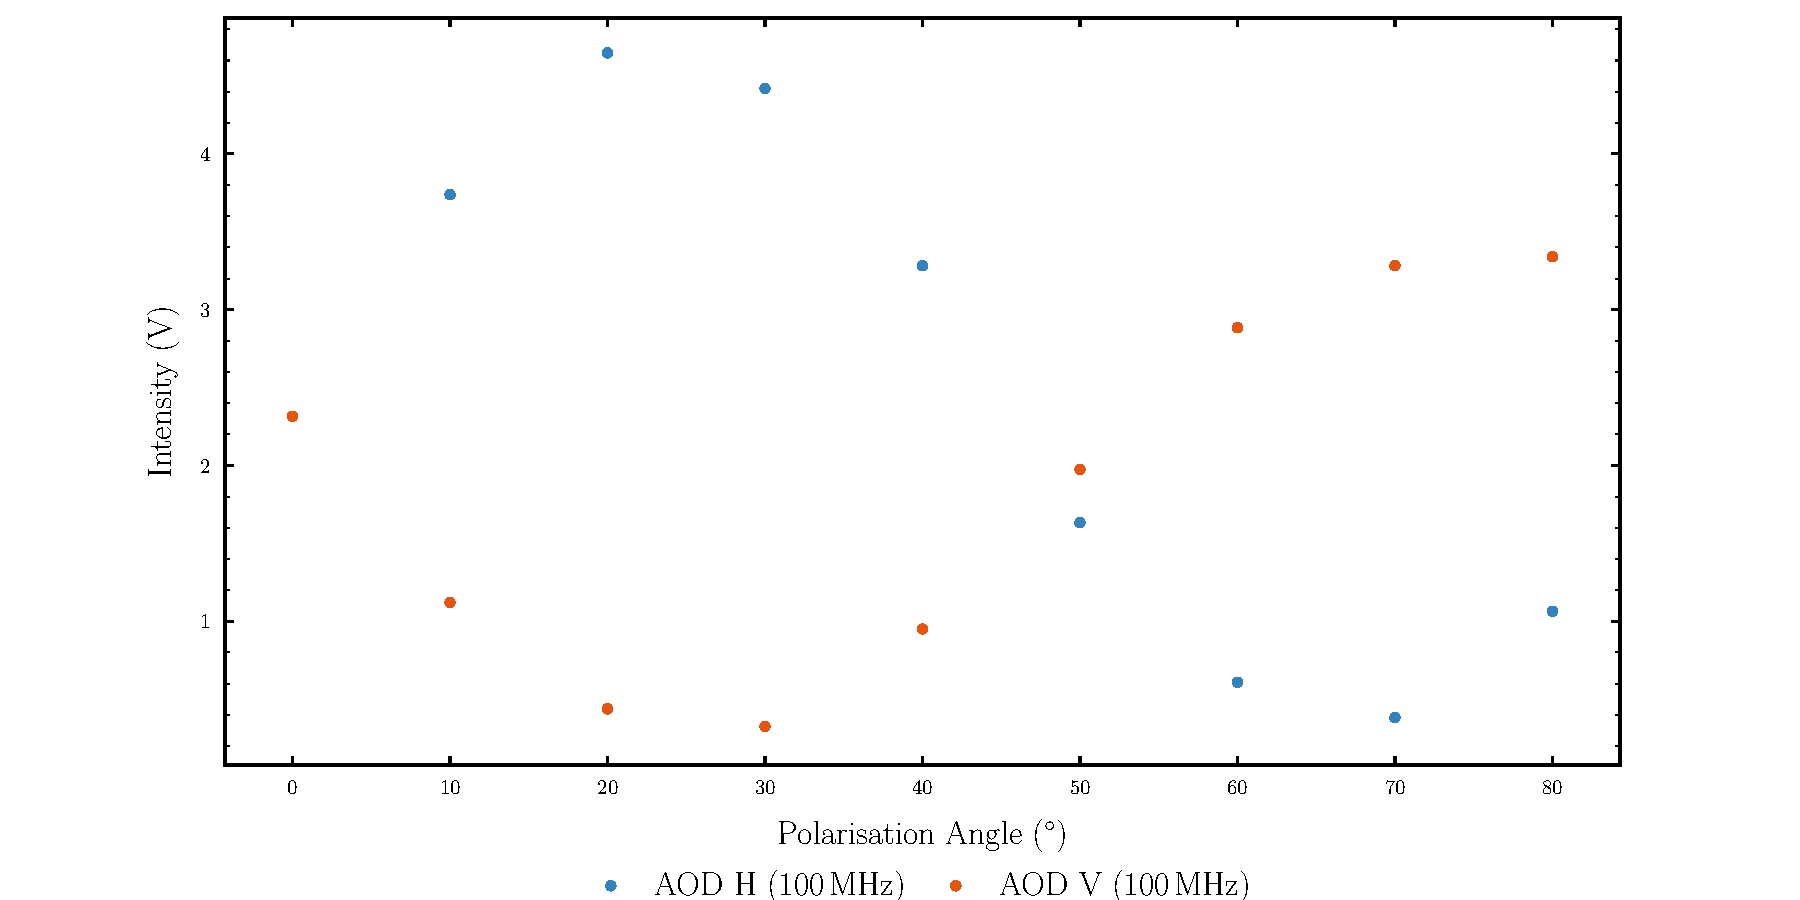
\includegraphics[width=\textwidth]
  {\figuredir{intensity/distribution/polarisation.pdf}}
  \captionsetup{width=.8\textwidth}
  \caption{Intensity transmission of the \gls{h} and \gls{v} \gls{aod} at
    \SI{100}{\mega\hertz} and maximum output amplitude for different
    polarisation angles.
  }\label{fig:intensity_polarisation}
\end{figure}
Finally we want to compare the polarisation angles between the individual
\gls{aod}s. Therefore we extracted the intensity transmission at
\SI{100}{\mega\hertz} frequency for both \gls{aod} measurements and plotted
them against the polarisation angle in \Cref{fig:intensity_polarisation}. We
observe a sinusoidal shaped intensity response of the polarisation angle
for the \gls{h} and \gls{v} \gls{aod} which seem out of phase by nearly
\ang{90}.

The 2D \gls{aod} casing allows to rotate the individual \gls{aod} elements. So
far we choose the rotation angle of the \gls{aod} elements that maximizes the
intensity transmission at the center frequency. What would we obtain if we
tilted the rotation angle a bit to the left and to the right?
\begin{figure}[htb]
  \centering
  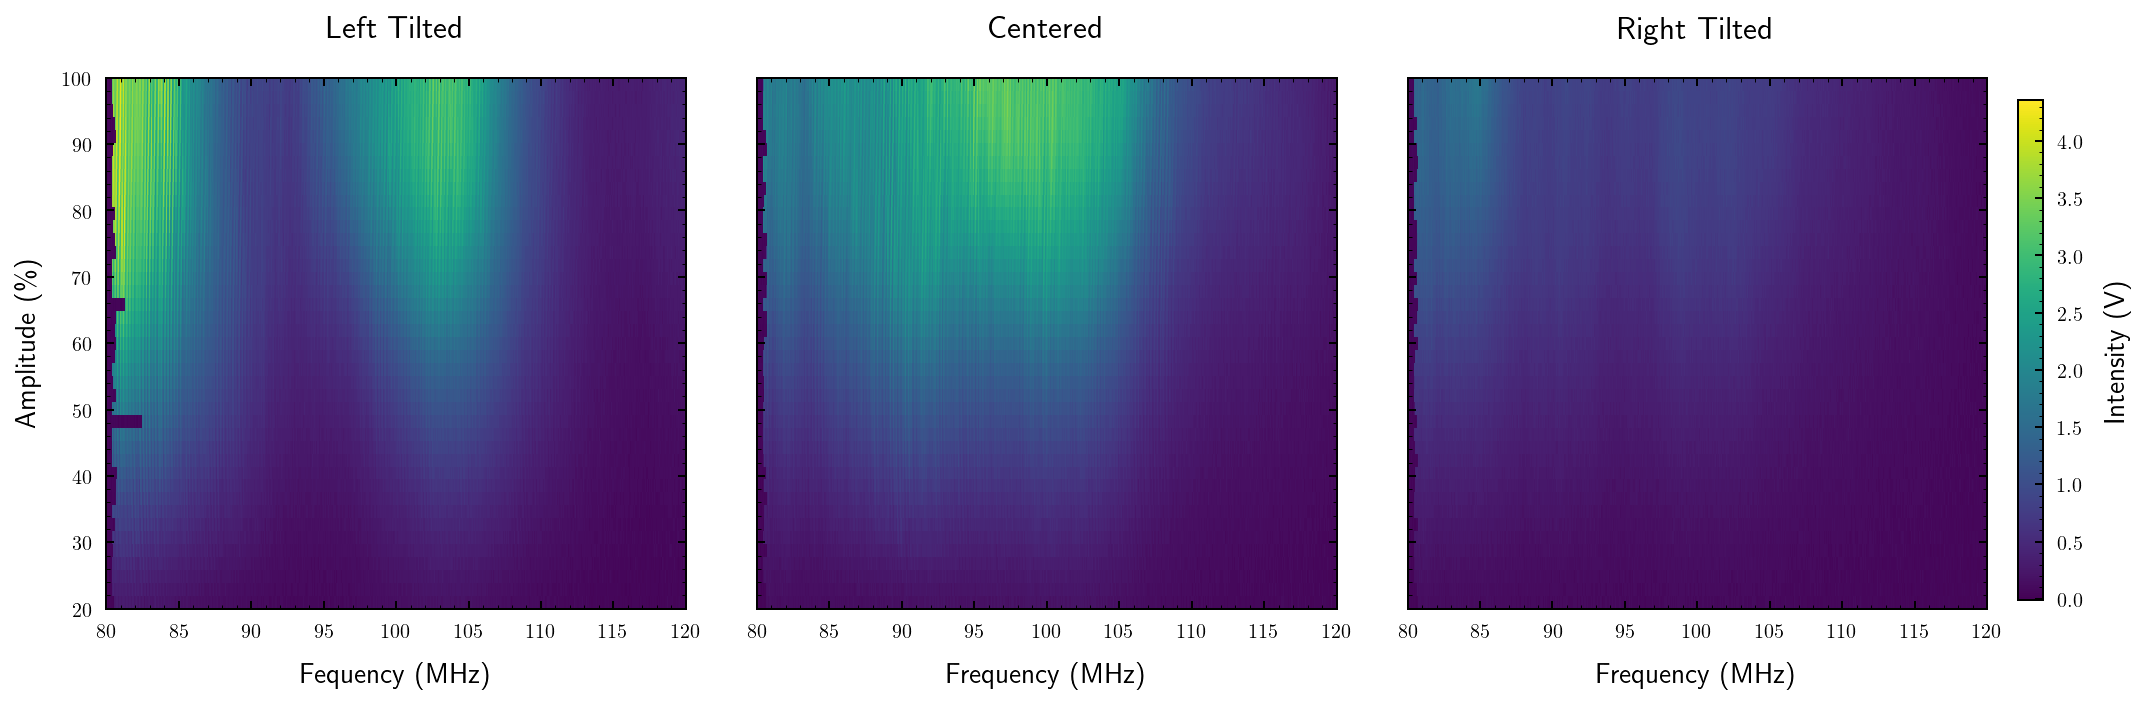
\includegraphics[width=\textwidth]
  {\figuredir{intensity/distribution/unpaired-tilted.png}}
  \captionsetup{width=.8\textwidth}
  \caption{Intensity distribution at different amplitudes for tilted
    individual \gls{aod}. We observe that the intensity decreases if the
    incident angle deviates from \ang{90}.
  }\label{fig:intensity_distribution_tilted}
\end{figure}
In \Cref{fig:intensity_distribution_tilted} we find the answer to this
question. We observe changes in shape and overall intensity with respect
to the incident angle. We should note that small changes in the incident
angle cause already large deflections of the beam, thus it is not guaranteed
that the left and right measurements are free from aperture effects.
Nevertheless we can record that the incident beam angle is an important
parameter in the intensity transmission of the \gls{aod}s. In particular we
need to consider the incident beam angle for the 2D \gls{aod} configuration.
It may make sense to change the setup to a configuration consisting of two
1D \gls{aod} with a telescope in between.

\subsection{Paired acousto-optic deflectors}

The \gls{aod} elements differ significantly in their intensity transmission
in between and with respect to their position. We find the horizontal element
in the anticipated horizontal position to have a significantly higher
transmission then any other configuration. Therefore we presume that the
\gls{aod} elements have a very high polarization dependency and are concerted
to eachother. We may find more evidence for this hypothesis by mounting both
\gls{aod} elements in their intended and exchanged slots.
\begin{figure}[ht]
  \centering
  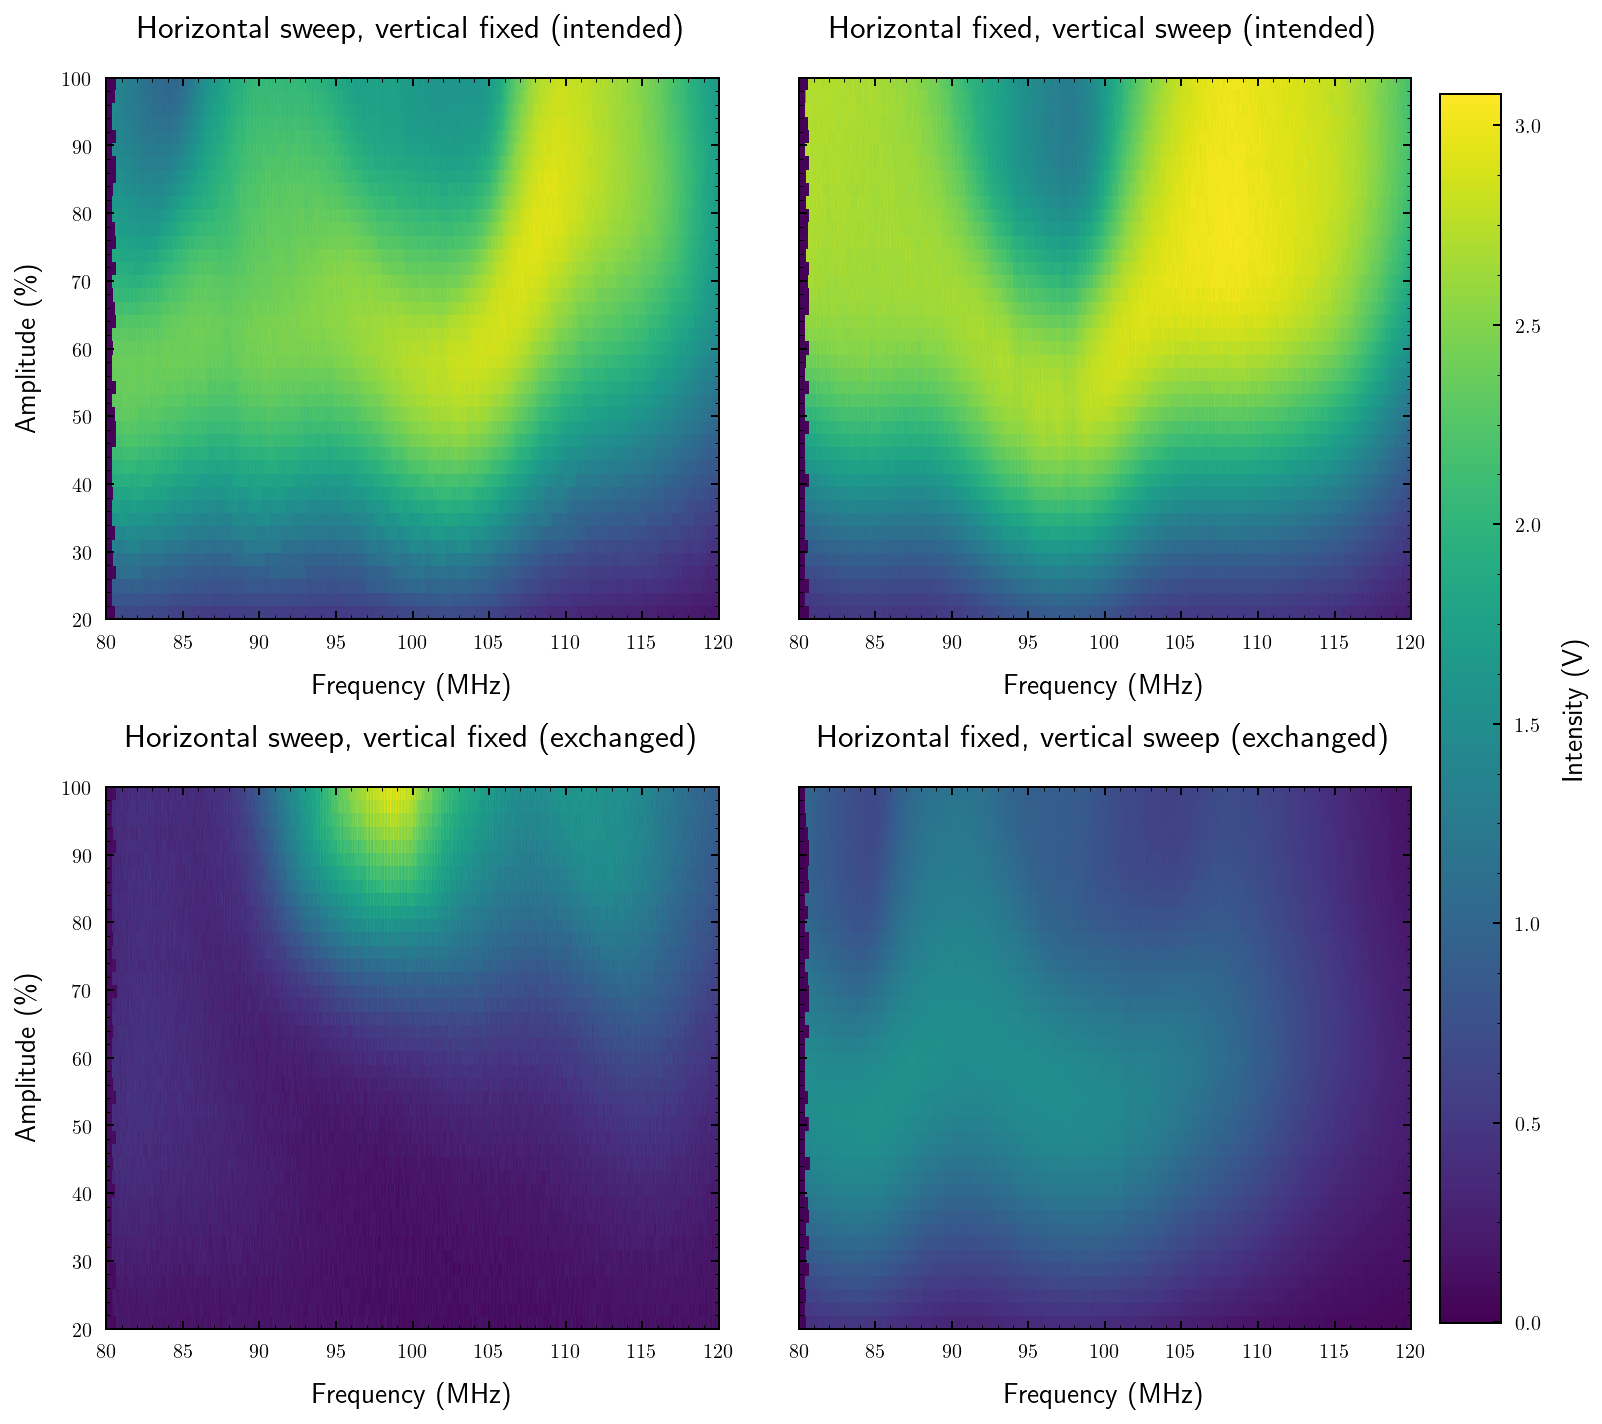
\includegraphics[width=\textwidth]
  {\figuredir{intensity/distribution/paired-amplitude.png}}
  \captionsetup{width=.8\textwidth}
  \caption{Intensity distribution over linear frequency sweep at different
  configured \gls{dds} amplitudes for different individual \gls{aod}
  configurations.
  }\label{fig:intensity_distribution_paired}
\end{figure}
In \Cref{fig:intensity_distribution_paired} the measured voltage of the
second photodiode are visualized in a two-dimensional heatmap. The horizontal
axis represents the frequency of the \gls{rf} signal applied to the \gls{aod}
elements whereas the vertical axis the configured \gls{dds} relative
amplitude. In the first row the elements where in their intended slots whereas
we exchanged them for the second row. In the first column the frequency
sweep was applied such that the beam moves along the horizontal axis while
in the second column the frequency sweep was applied to the element that
causes beam movement in the vertical direction.

We see that for the exchanged positions the transmission is reduced and
asymmetric with respect to the sweep direction whereas the elements in their
intended position perform better in every aspect. We therefore conclude that
the \gls{aod} are cut in a intended way to account among others for
polarization effects and it is advised to operate them in their anticipated
slot as we will do for all following experiments.

\section{2D intensity distribution}

In the previous section we sorted out the influence of the \gls{aod} element
position and acknowledged that \gls{aod}s differ significant in their
optical properties. In the present section we now want to explore the
intensity transmission for a two dimensional sweep as intended to be used
for the optical potentials.

The experimental setup is similar to the previous setups and is shown in
\Cref{fig:intensity_distribution_setup}. We have both \gls{aod}s mounted in
their anticipated position. The \gls{aod} elements are aligned to maximize
intensity at the center frequency. The laser beam is directed into a second
photodiode where we measure the intensity with respect to the configured
\gls{dds} signal.
\begin{figure}[ht]
  \centering
  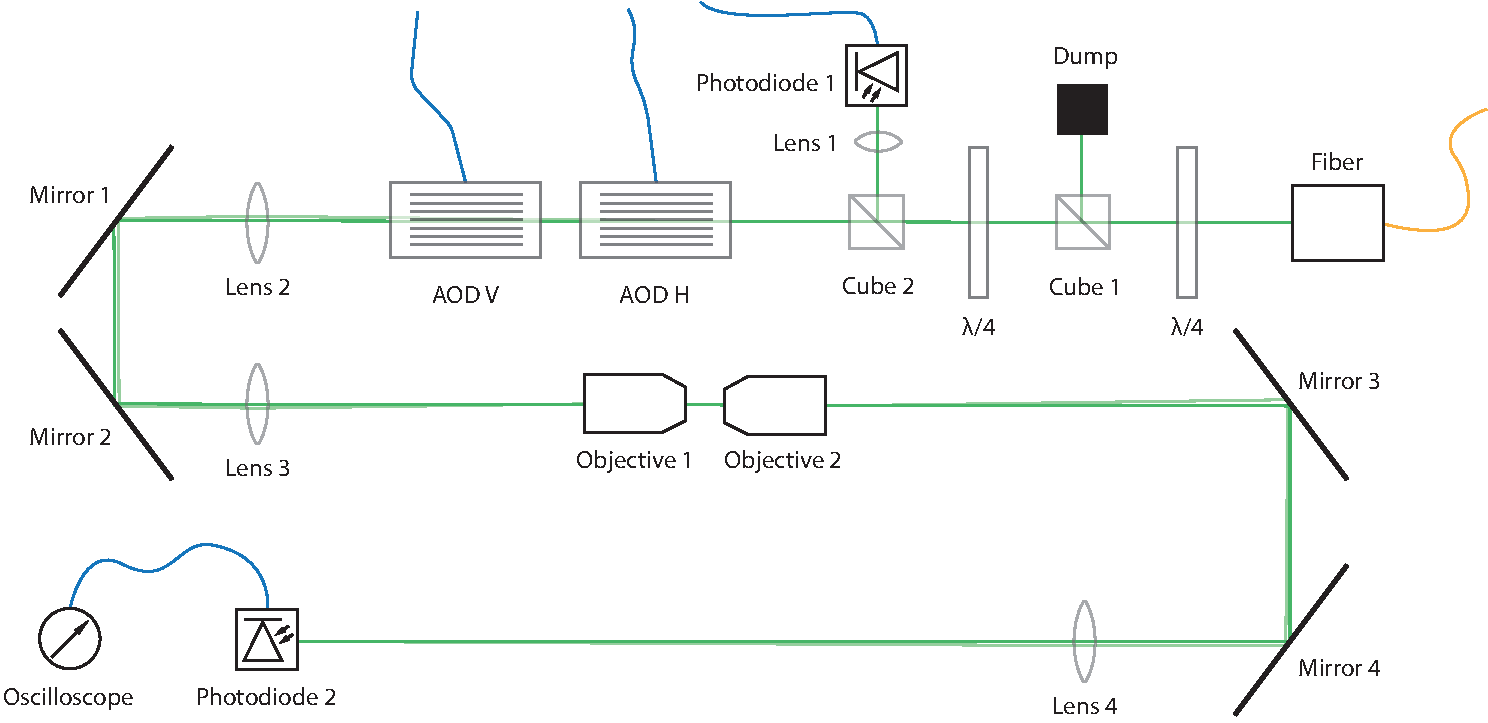
\includegraphics[width=\textwidth]{\mediadir{setup/intensity-distribution.pdf}}
  \captionsetup{width=.8\textwidth}
  \caption{Experimental setup used to measure the intensity transmission of
    the 2D \gls{aod} in dependence of the configured \gls{dds} signal.
  }\label{fig:intensity_distribution_setup}
\end{figure}

\subsubsection{Digital ramp frequency sweep}

In a first attempt we configure a first \gls{dds} to output a constant
frequency whereas a second \gls{dds} is configured to do a frequency sweep
using the internal digital ramp. After one such sweep the constant frequency
output of the first \gls{dds} is increased and the measurement repeats. The
procedure is repeated until the first \gls{dds} covered the same frequency
range as the second \gls{dds}.
\begin{figure}[ht]
  \centering
  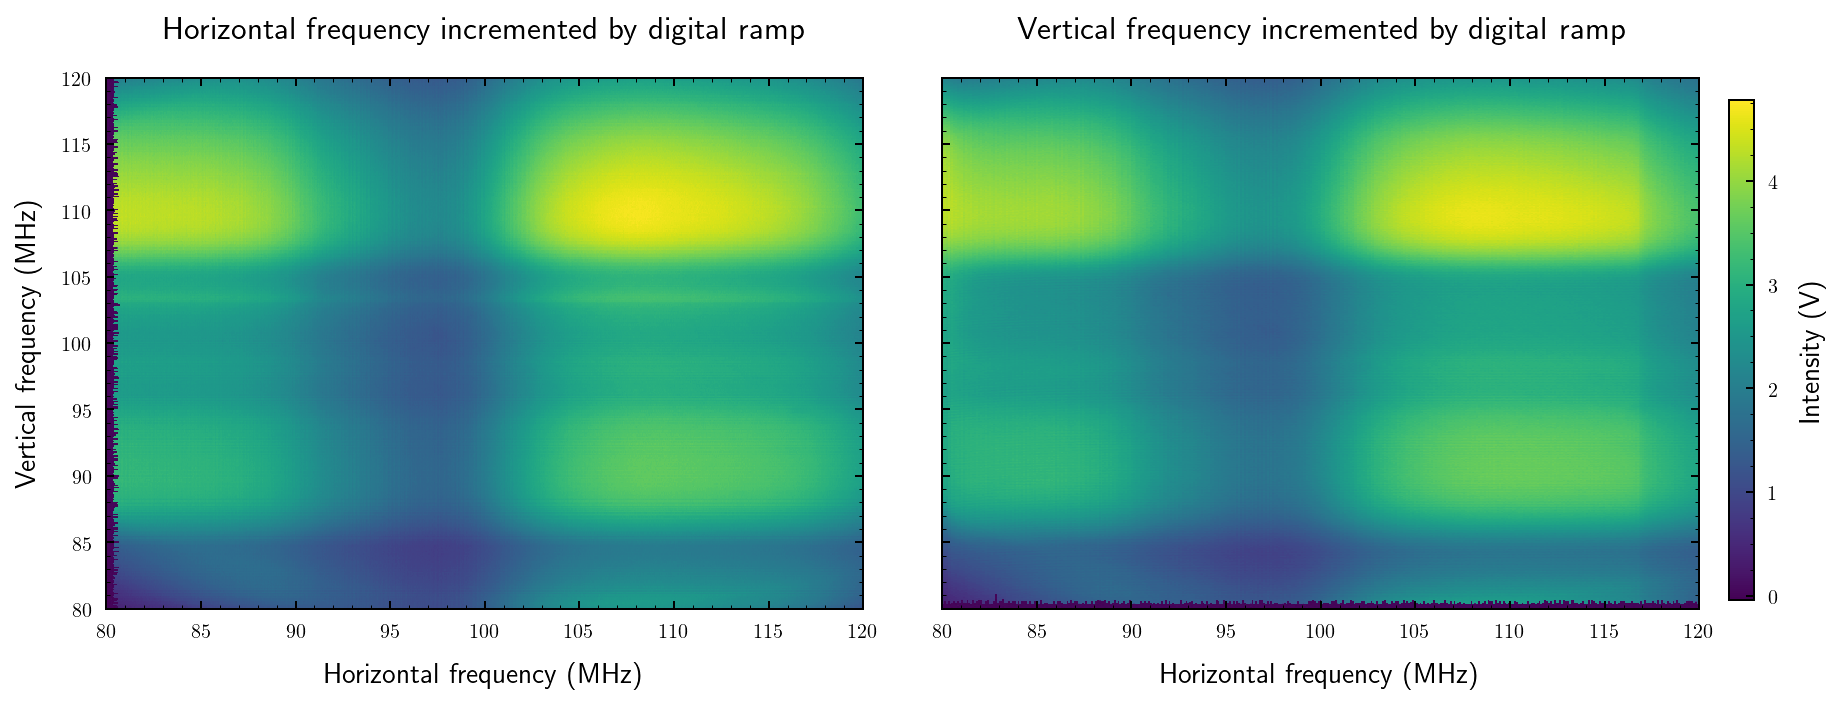
\includegraphics[width=\textwidth]
  {\figuredir{intensity/distribution/paired-frequency.png}}
  \captionsetup{width=.8\textwidth}
  \caption{Intensity measured as voltage at the photodiode in dependence of
    the horizontal and vertical applied frequency signal to the \gls{aod}. The
    left map is obtained by enabling the digital ramp on the horizontal
    \gls{dds} whereas the vertical \gls{dds} is configured to output a
    constant frequency which is manually increased after each measurement.
    On the right-hand side map the roles are exchanged.
  }\label{fig:intensity_distribution_frequency}
\end{figure}
In \Cref{fig:intensity_distribution_frequency} we present the intensity
measured at the second photodiode in the setup shown in
\Cref{fig:intensity_distribution_setup}. On the left-hand map the first
\gls{dds} is the \gls{dds} responsible for translations in vertical direction
whereas the second \gls{dds} is responsible for translations in horizontal
direction. The frequency sweep performed by the digital ramp is more dense
compared to the frequency sweep performed by manual increments in our
configuration as the manual increments require driver calls whereas the
digital ramp increments are performed internal of the \gls{dds}.
\begin{figure}[ht]
  \centering
  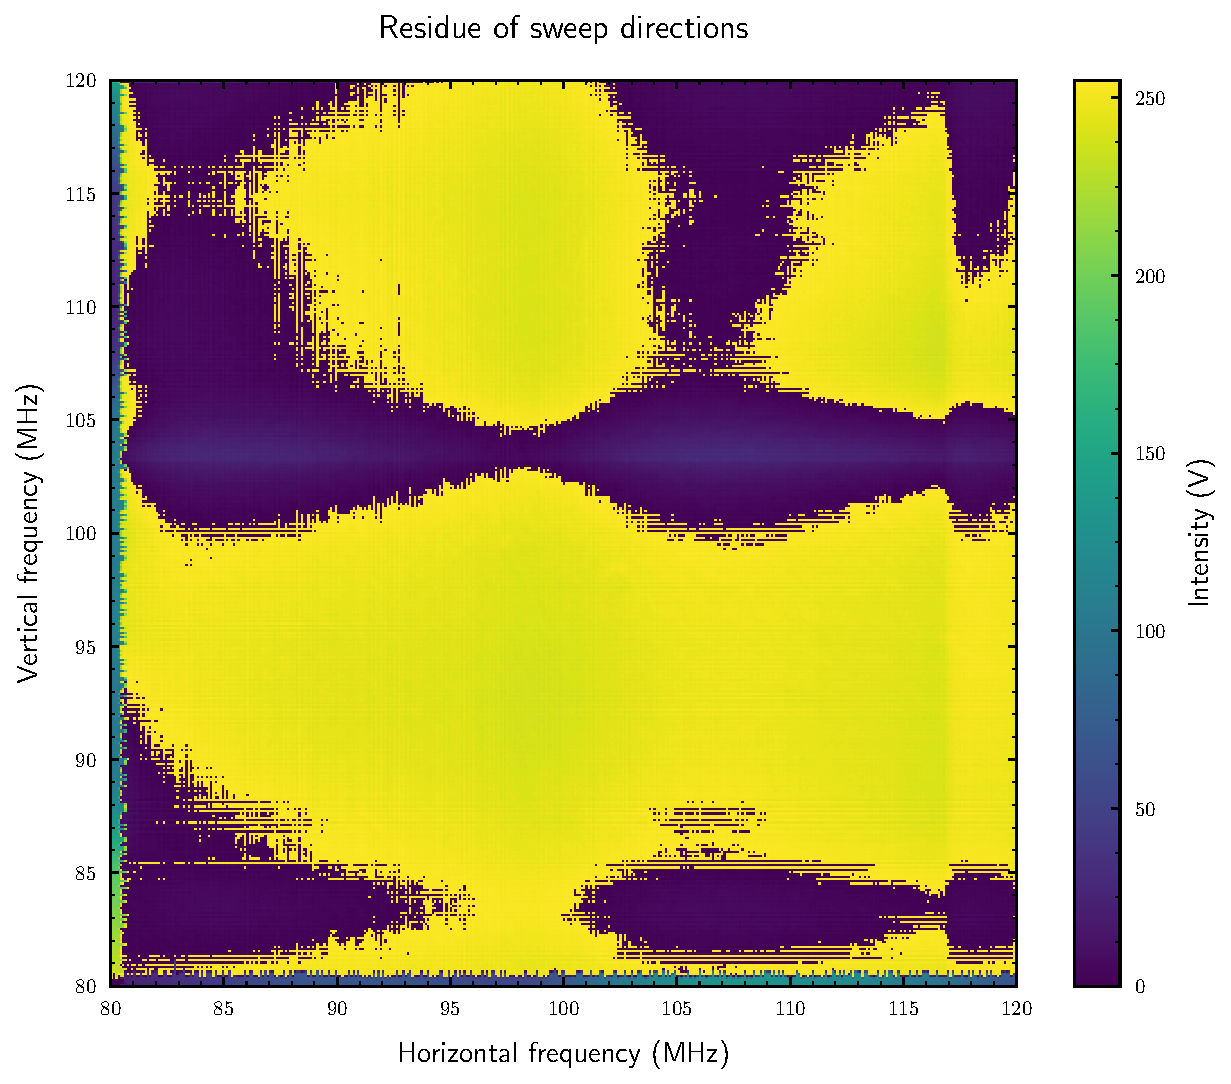
\includegraphics[width=.7\textwidth]
  {\figuredir{intensity/distribution/paired-frequency-residue.pdf}}
  \captionsetup{width=.9\textwidth}
  \caption{Absolute difference between the 2D intensity distribution
  performed with the digital ramp configured set to different axes.}
  \label{fig:intensity_distribution_frequency_residue}
\end{figure}
As the differences in \Cref{fig:intensity_distribution_frequency} are of only
subtile nature we additionally reveal the absolute difference between both
maps in \Cref{fig:intensity_distribution_frequency_residue}. We observe
nearly a binary map of dark purple and yellow areas whereas the dark area can
be intepreted as small and the yellow area as large difference. The binary
nature of the absolute difference could be interpreted as a fixed offset
in the power level between the \gls{h} and \gls{v} \gls{rf} signal supplied to
the \gls{aod}s. In areas of small intensity difference (purple) the ouptut
level may be sufficient to saturate the acousto-optics. However we must admit
that these are simply suggestions and need further evidence.

\subsubsection{Constant sampled frequencies}

In \cref{subsec:electronic_amplitude_frequency_response} we did not find
differences in the amplitude frequency response of the amplified \gls{rf}
signal between frequency increments performed by the internal digital ramp of
the \gls{dds} and frequency increments performed by manually updating the
output frequency through the driver. Yet, it remains open if differences
arise in the transmission frequency response of the \gls{aod} as the \gls{aod}
is not a purely electronic device.
\begin{figure}[ht]
  \centering
  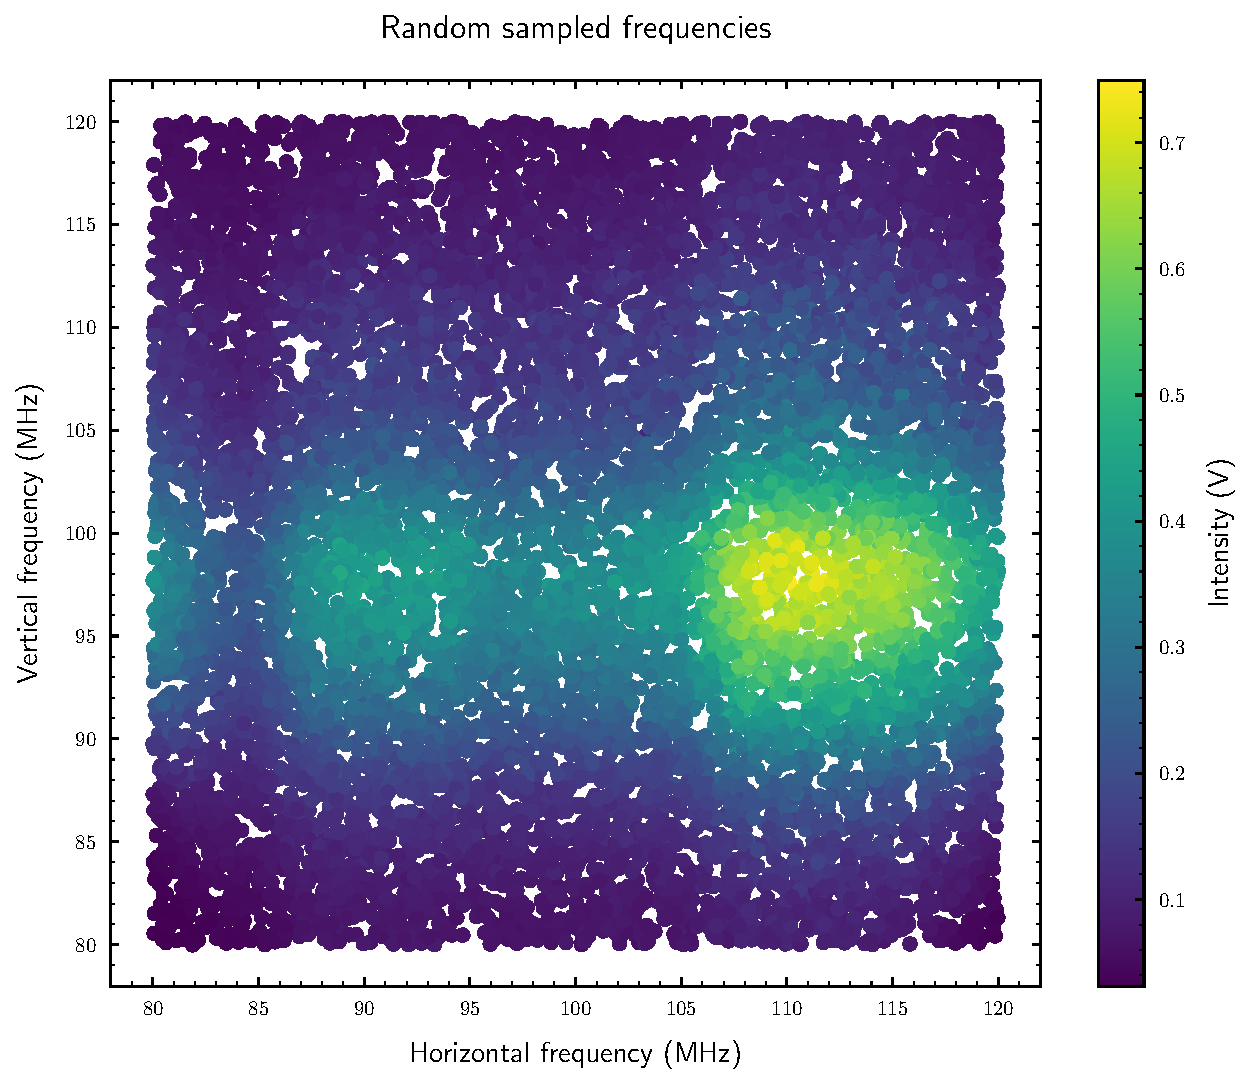
\includegraphics[width=.7\textwidth]
  {\figuredir{intensity/distribution/sample-frequency.pdf}}
  \captionsetup{width=.9\textwidth}
  \caption{Intensity measured as voltage at the photodiode in dependence of
    the horizontal and vertical applied frequency signal to the \gls{aod}.
    Frequency pairs are sampled over a uniform distribution and then passed
    as constant output frequency paramter to the \gls{dds}.
  }\label{fig:intensity_distribution_frequency_sampled}
\end{figure}
To partly answer this question we sampled random frequency pairs over a
two dimensional uniform distribution and passed them as constant frequency
parameter to the respective \gls{dds} through the driver interface. The
yielded intensity distribution is visualized in
\Cref{fig:intensity_distribution_frequency_sampled}. We note that in
comparison to \Cref{fig:intensity_distribution_frequency} the intensity
differences are more concentrated around the vertical axis. We believe that
acousto-optics possess a non-instantaneous frequency response characteristic
that requires further investigation.

\subsubsection{Different radio frequency signal source}

In the previous two sections we found that the \gls{aod}s are quite sensible
to the method used to perform frequency increments in a frequency sweep. In
order to further investigate this phenomena we decided to replace one
\gls{dds} with a high-quality signal generator while the other \gls{dds} was
configured to output a constant \SI{100}{\mega\hertz} signal. The output
level of the signal generator was configured to match the output level of
the \gls{dds} and amplified using the usual power amplifier.
\Cref{fig:intensity_distribution_signal_sources} discloses the different
intensity transmission registered by the photodiode for a frequency sweep
performed by the \gls{dds} through the digital ramp and by the signal
generator. In comparison to the \gls{dds} the signal generator does not
support continous frequency changes as we can see from the intensity drops
between the frequency increments of the signal generator trace.
\begin{figure}[ht]
  \centering
  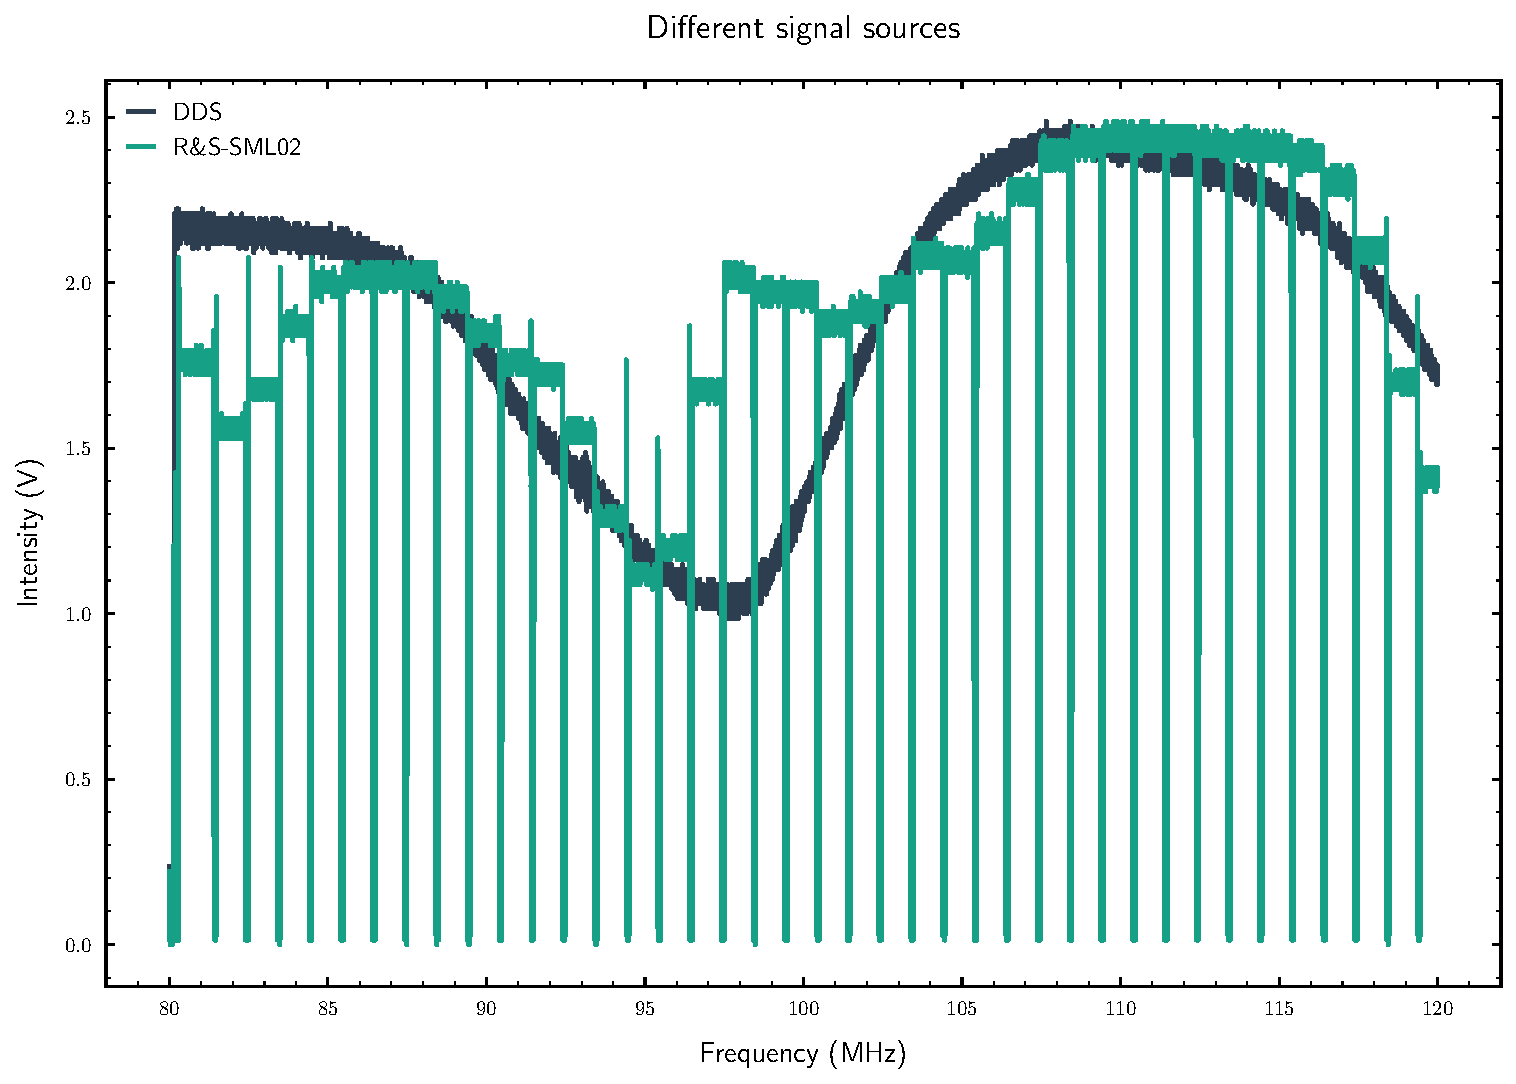
\includegraphics[width=.9\textwidth]{\figuredir{intensity/distribution/signal-sources.pdf}}
  \captionsetup{width=.9\textwidth}
  \caption{Intensity measured as voltage at the photodiode with one \gls{aod}
    at constant center frequency supplied by a \gls{dds} and the other
    \gls{aod} performing a linear frequency sweep with the \gls{dds} and a
    high-quality signal generator.
  }\label{fig:intensity_distribution_signal_sources}
\end{figure}
Further ignoring these intensity drops we observe that the global response
characteristics differ in particular at the begin of the frequency sweep and
at the center. As the power amplifier remains unchanged through the
measurements and the output voltage of the signal sources are independent of
frequency, we are only left with two explainations. For one the power supplied
to the \gls{aod} could differ as we did not meausre the current response. On
the other the frequency drops in between frequency increments of the signal
generator could cause the observed characteristis. The later hyphothesis would
also confirm the result of the previous section in which we found a different
transmission characteristic for differen frequency sampling strategies.

\subsubsection{Summary}

In summary we found that the intensity transmission of the \gls{aod} show a
highly non-linear dependency in the applied power and the method used for
frequency sampling. It will continue to be interesting to explore the
intensity transmission subject to the effective power of the \gls{rf} signal
applied to the \gls{aod}. So far we only know that the voltage of the \gls{rf}
signal of the \gls{dds} is constant over our frequency range of
\SI{80}{\mega\hertz} to \SI{120}{\mega\hertz}, however we cannot make any
statements with respect to the current characteristics. All in all there are
too many factors to consider to describe with a simple analytical model and we
will further try to work with a model-free optimization procedure in the next
chapter in order to minimize the intensity transmission variance and produce
a constant laser intensity in the atom plane.

\chapter{Intensity transmission optimization}

The previous two chapters addressed the characteristics of the \gls{rf}
signal and the intensity transmission of the \gls{aod}. Therewith the
groundwork has been set out to finally approach the mission of minimizing the
intensity variance to obtain a homogenous optical potential.

But how do we minimize the intensity variance? The \gls{dds} permits to read
$N=1024$ amplitude values from memory. The optimization problem therefore is to
minimize the variance of the intensity distribution $I(A)$ subject to an
amplitude vector $A\in[0,1]^N$. The conclusions drawn from the intensity
measurements suggest that we have to expect non-linear, irregular behaviour
in $I(A)$. and indeed first attempts to model $I(A)$ through polynomial fits,
multilayer perceptron networks and least-squared minimizations have failed.

During these optimization procedures we observed that changing an amplitude
value $A_i\in A$ does affect the intensity voltage at subsequent
$A_{i+1},\dots,A_N$. Fortunately we found that by respecting the amplitude
order with respect to increasing frequency during optimization we where able
to bypass these effects. Further we created amplitude segments
$\left(A_j,\dots,A_{j+m}\right)$ consisting of $m$ ordered amplitude values
to reduce the optimization time. Optimization then was performed through
random search which was proven to yield better results as grid search
\cite{Bergstra2012}.

\subsubsection{Overview}

First, we want to provide an overview of the final optimization results
obtained at different hyperparameters for the random search. The
hyperparameter includes the number of amplitude segments $N/m$ and the target
intensity.
\begin{figure}[ht]
  \centering
  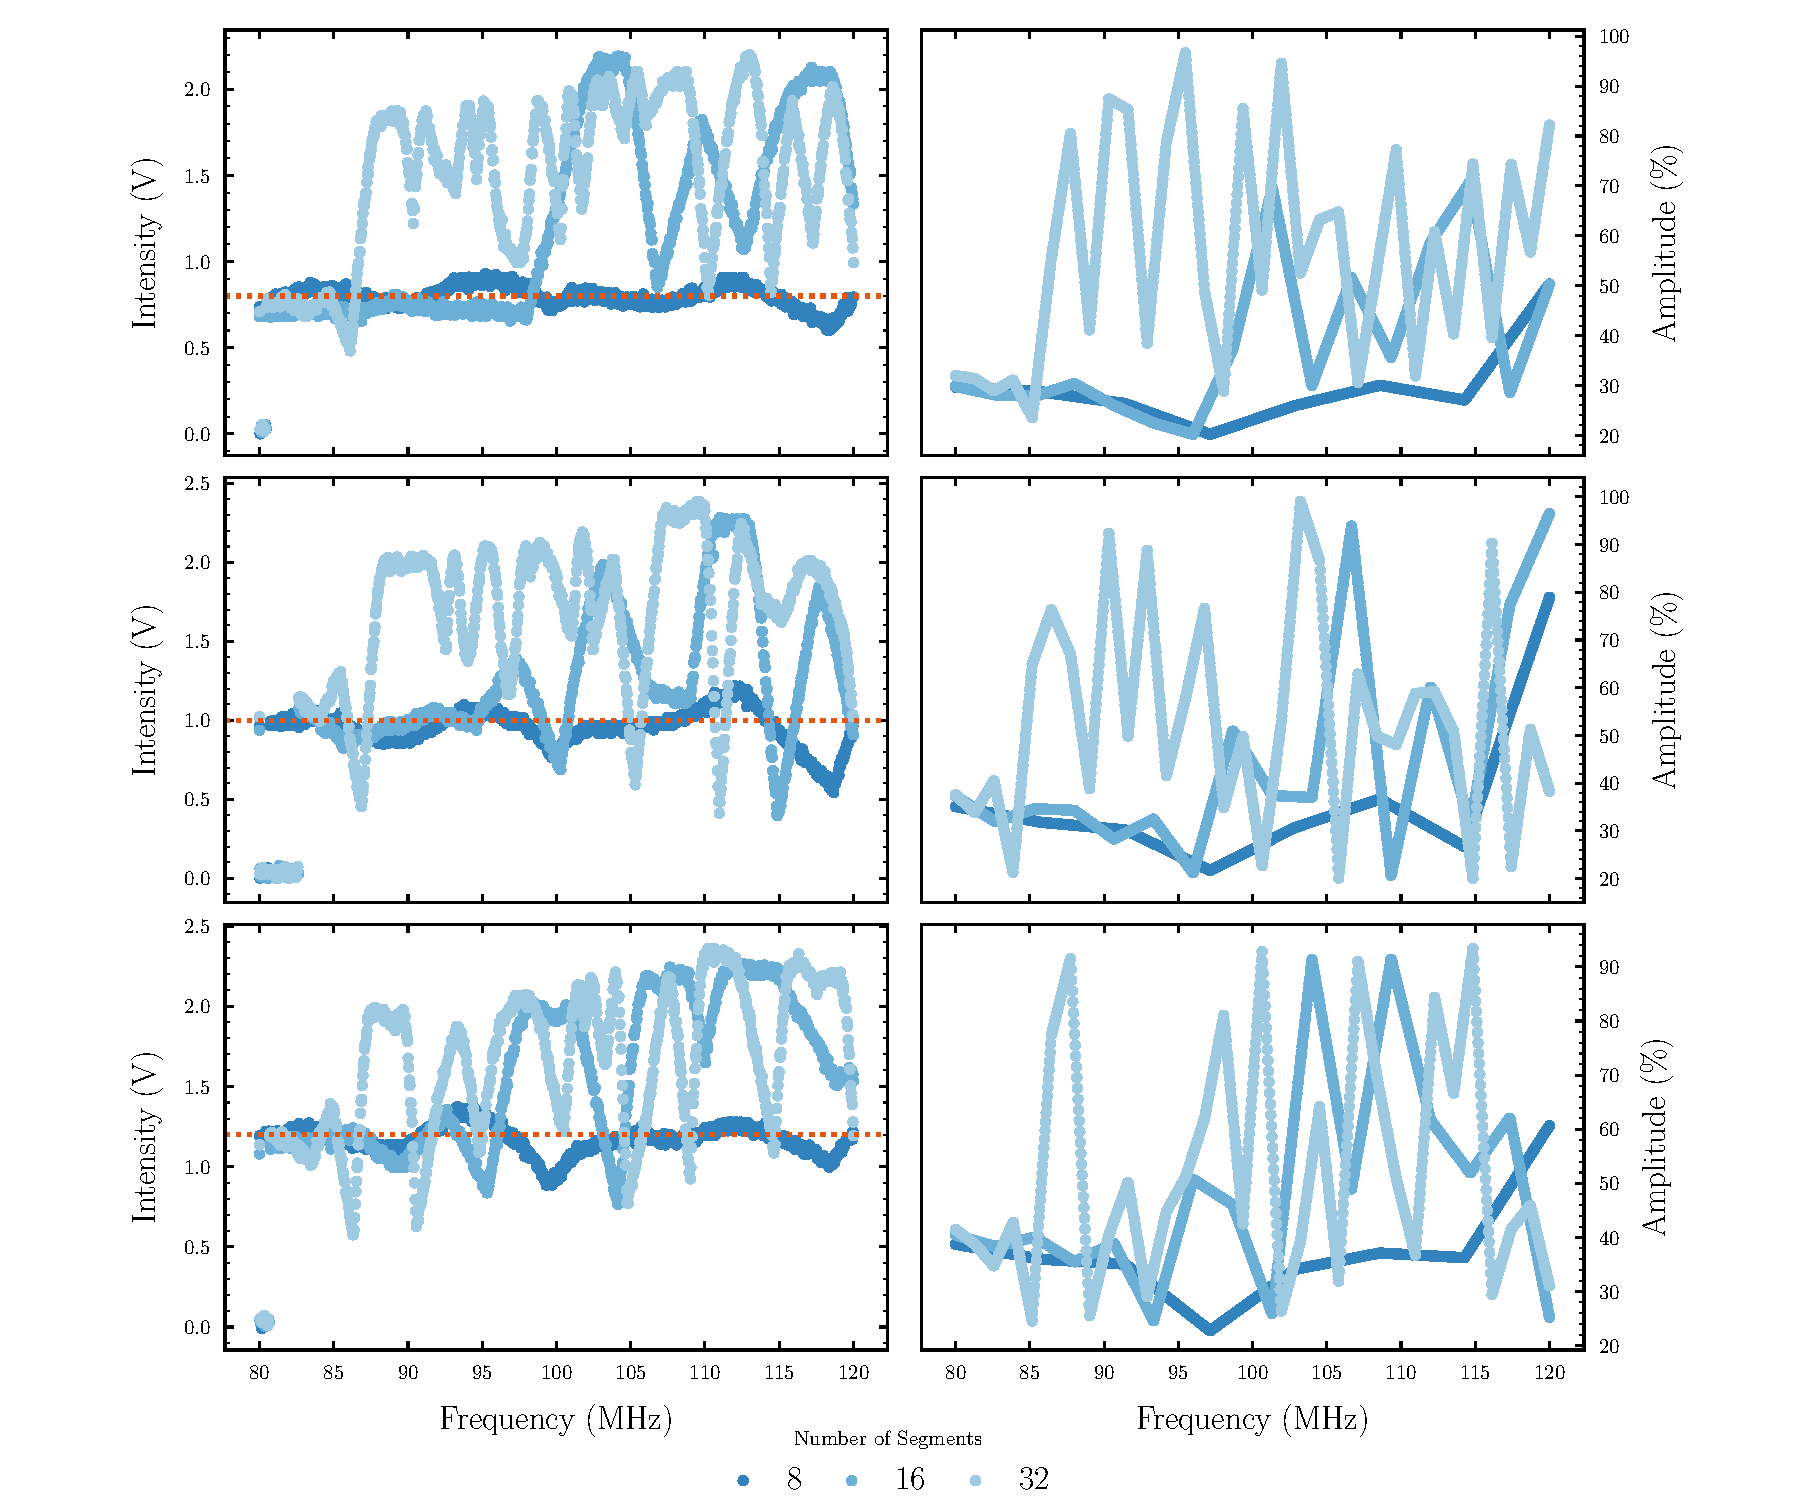
\includegraphics[width=\textwidth]{\figuredir{intensity/optimization/overview.pdf}}
  \captionsetup{width=.8\textwidth}
  \caption{Minimized intensity variance for different target intensities
  and number of amplitude segments. We note heavy oscillations for
  amplitude segments greater than eight.}
  \label{fig:intensity_optimization_overview}
\end{figure}
In \Cref{fig:intensity_optimization_overview} we present the final
optimization results for target intensities of \SI{800}{\milli\volt},
\SI{1000}{\milli\volt} and \SI{1200}{\milli\volt} and amplitude segments
$8,16,32$. We observe heavy oscillations for amplitude segments greater than
eight. The optimization results using 16 amplitude segments performs better
than the run with 32 amplitude segments.

We assume that inductive effects occur when choosing more amplitude segments
that consolidate a non-linear intensity response. For the sake of simplicity
we will first limit us to the case of eight amplitude segments.

\begin{figure}[ht]
  \centering
  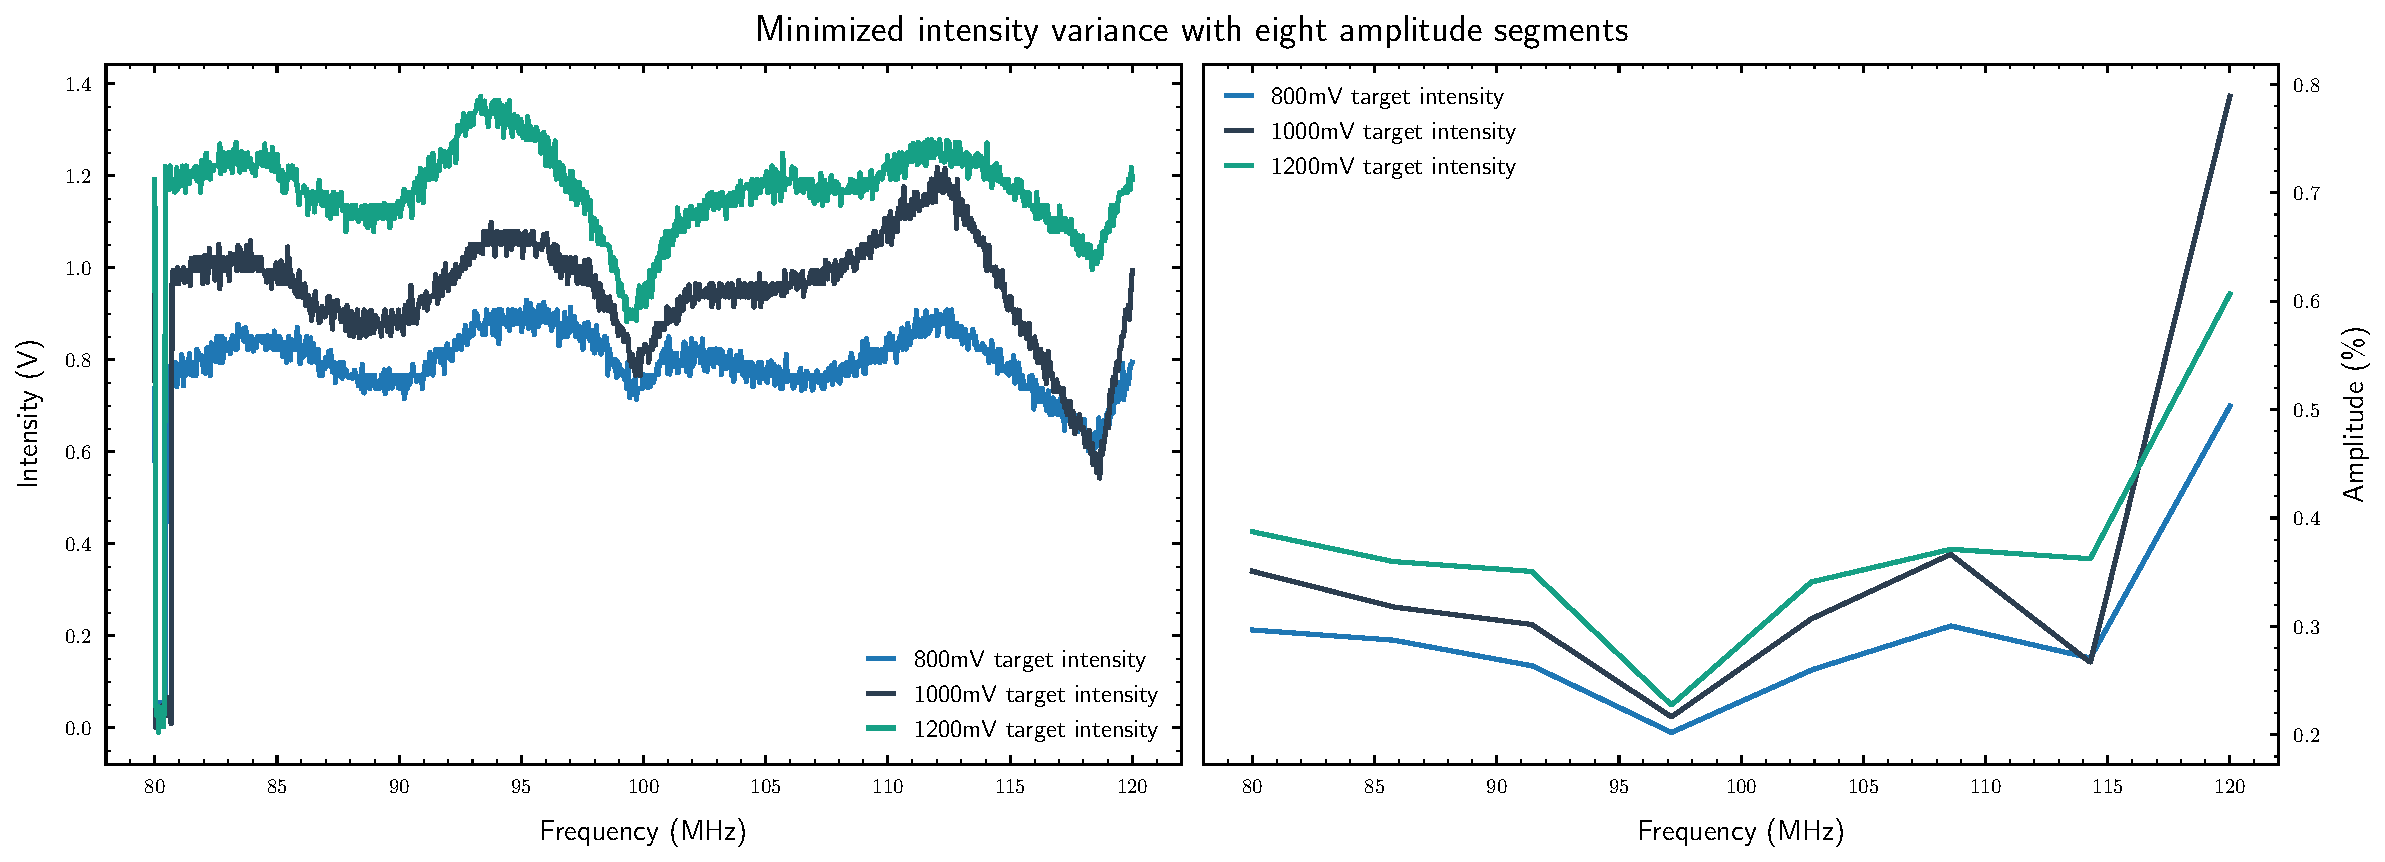
\includegraphics[width=\textwidth]{\figuredir{intensity/optimization/intensity-amplitude.pdf}}
  \captionsetup{width=.8\textwidth}
  \caption{Final result of the intensity variance minimization and the
  corresponding amplitude segment values obtained through random search with
  eight independent amplitude segments.}
  \label{fig:intensity_optimization_intensity_amplitude}
\end{figure}

In \Cref{fig:intensity_optimization_intensity_amplitude} we have a closer
view on the first column of \Cref{fig:intensity_optimization_overview}. We
can notice similar characteristics observed in the \gls{rf} signal. In
particular the more power drop near the center frequency is present and the
linear power fall off with the frequency in the second half of the frequency
sweep.

\subsubsection{Process}

We now want to elaborate on the optimization process. We limit ourselves to
the optimization process with eight amplitude segments as it was the most
successful one and can be covered completly with eight plots.

\begin{figure}[ht]
  \centering
  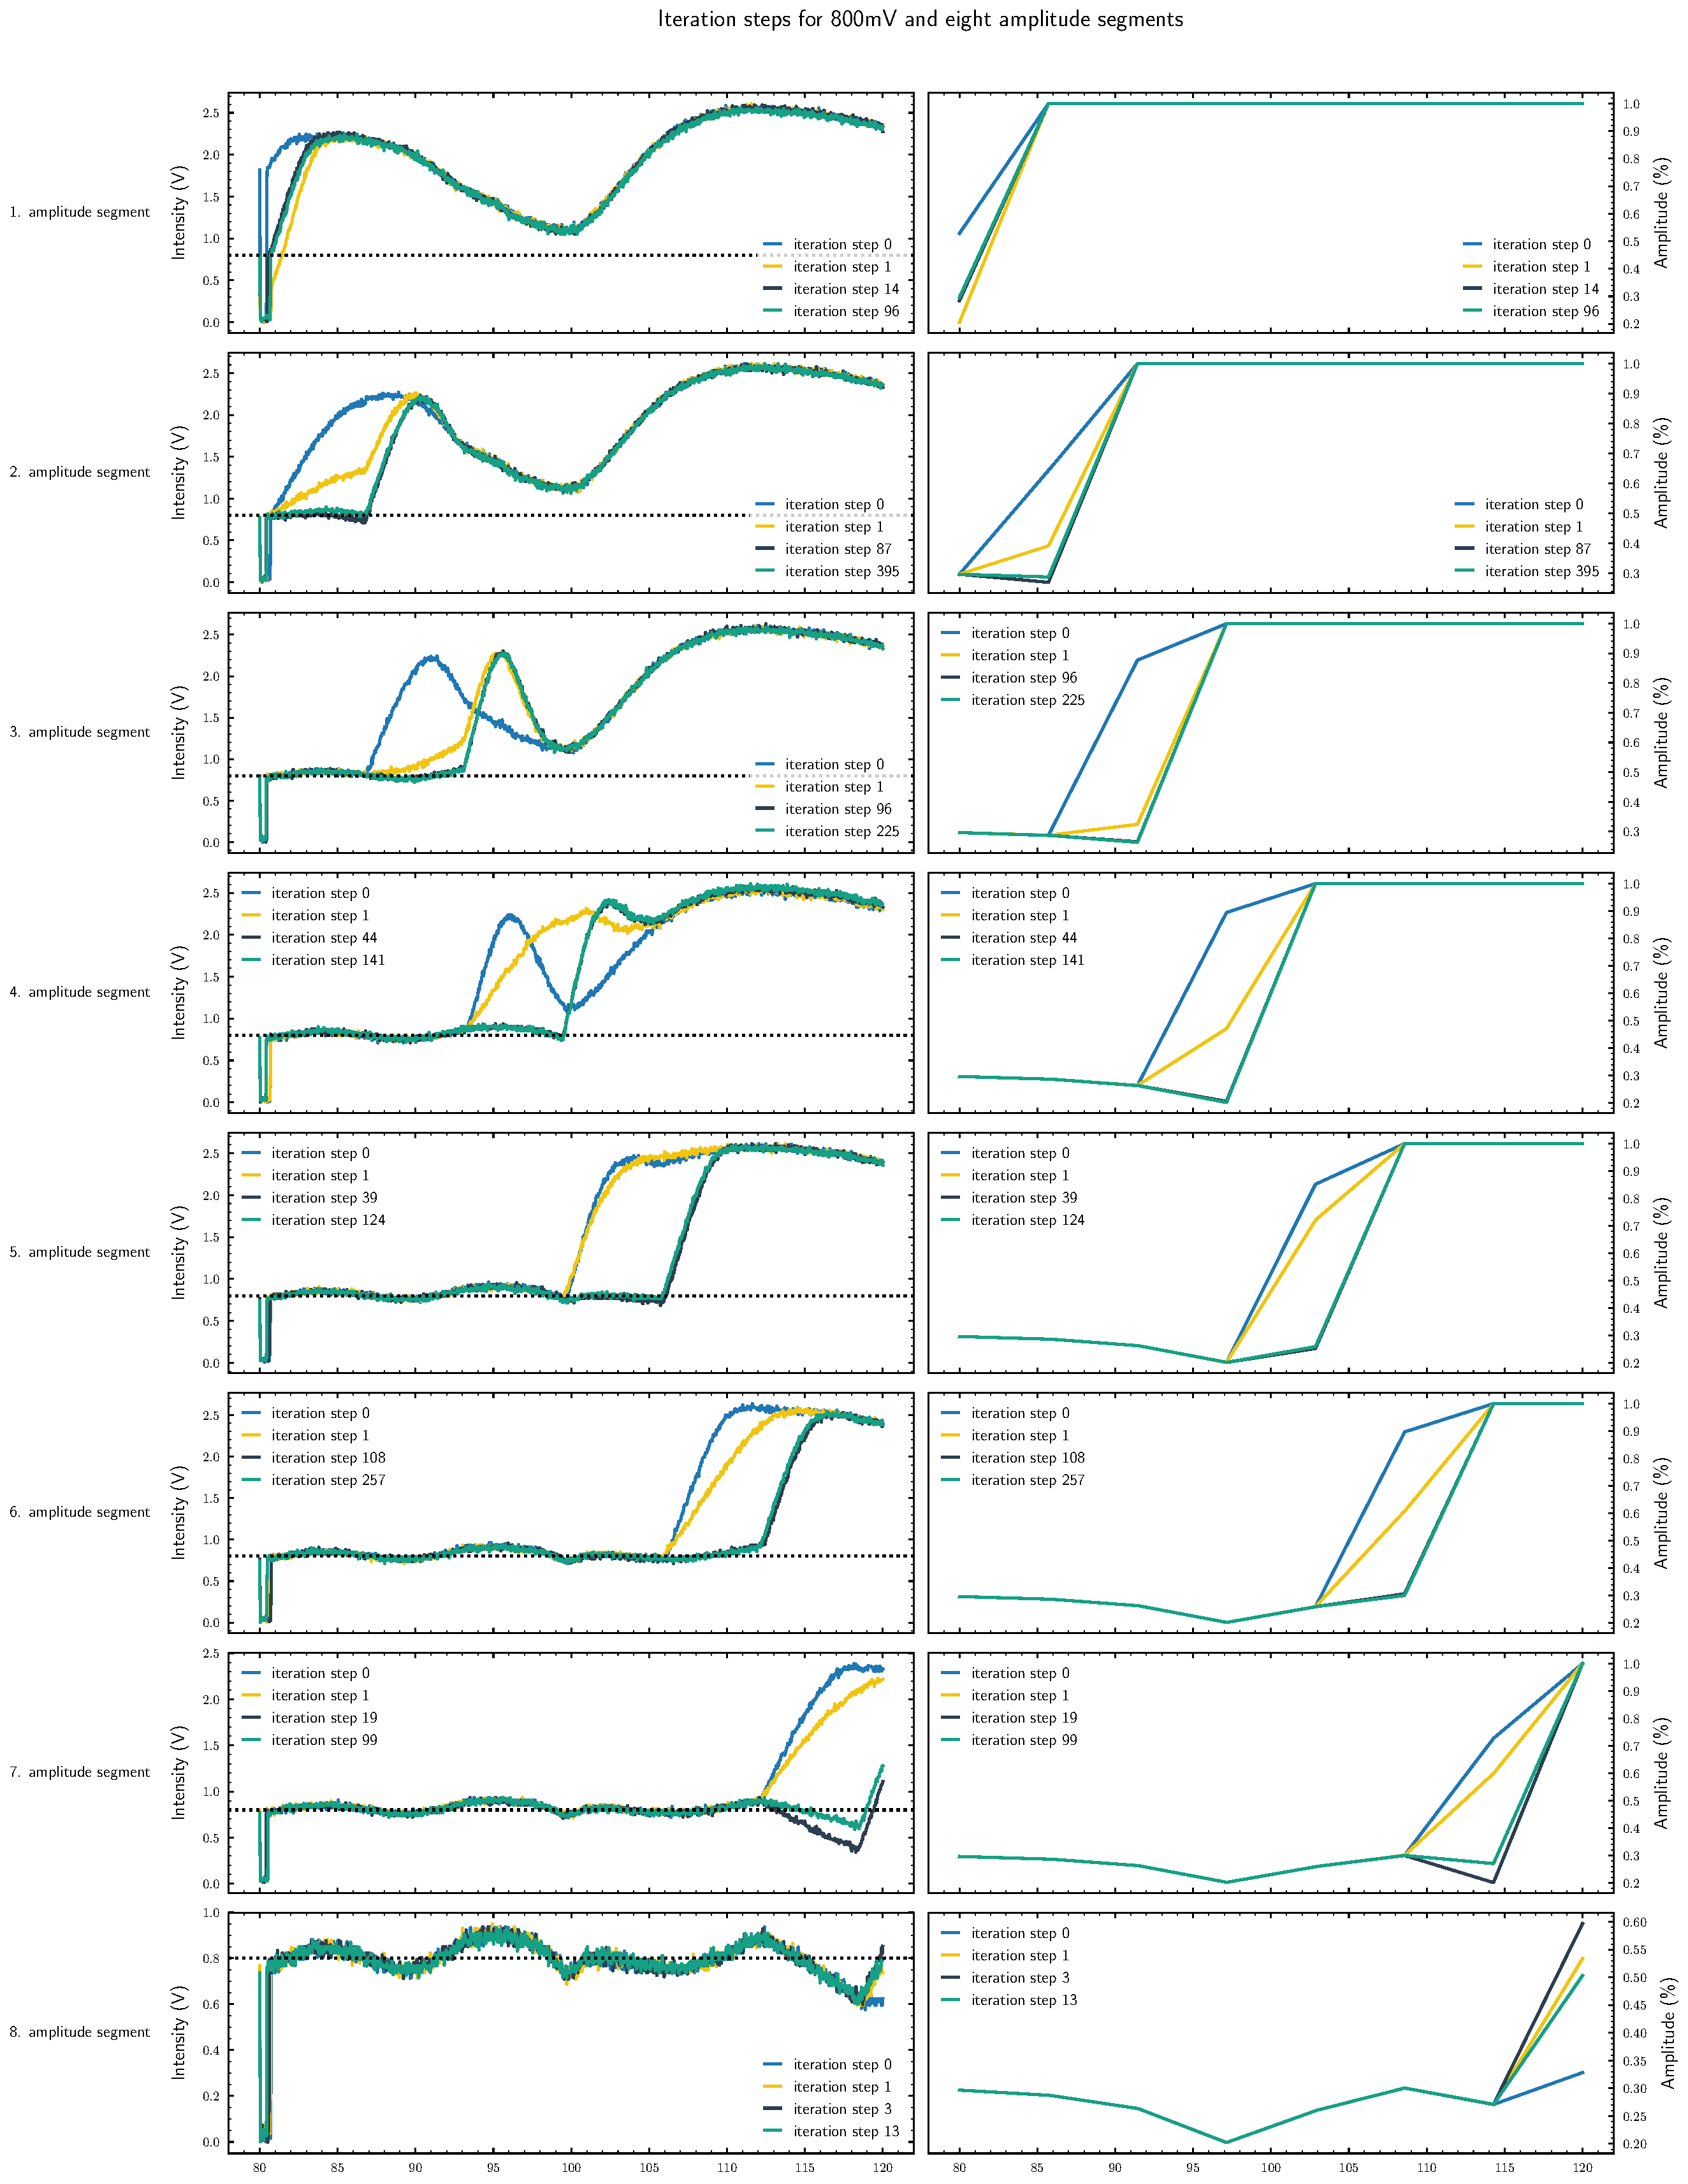
\includegraphics[width=\textwidth]{\figuredir{intensity/optimization/process.pdf}}
  \captionsetup{width=.8\textwidth}
  \caption{Intensity and amplitude at different stages of the optimization
  process. In each column a different amplitude segment is optimized.
  The different traces in each plot mark the respective iteration.}
  \label{fig:intensity_optimization_process}
\end{figure}

In \Cref{fig:intensity_optimization_process} we see the intensity and
amplitude at different optimization stages. At each stage one amplitude
segment is sampled from a uniform distribution over $[.2, .8]$. The intensity
segment associated with this amplitude segment is then used to calculate
the \gls{mse} and compare it to the previous best \gls{mse}. If the new
\gls{mse} is less than the previous best \gls{mse} the previous best \gls{mse}
is updated and the amplitude segment value is saved. This procedure is
repeated 500 times. Every time a new best value was found we saved the
data. For the diagrams we choose the four most separated iteration steps to
visualize the process of the optimization.

If we take a look at the succeeding segment from the currently optimized
amplitude segment we observe that these differ for different amplitude
values and henceforth confirms that amplitude values are not independent but
affect subsequent segments.

\subsubsection{Failure}

With the optimization showing reasonable convergence for eight amplitude
segments we would expect it to improve if we choose a more amplitude segments,
yet we observed heavy oscillations. In this section we want to check the
optimization process in the case of 32 amplitude segments to investigate in
possible origins of the optimization failure.

\begin{figure}[ht]
  \centering
  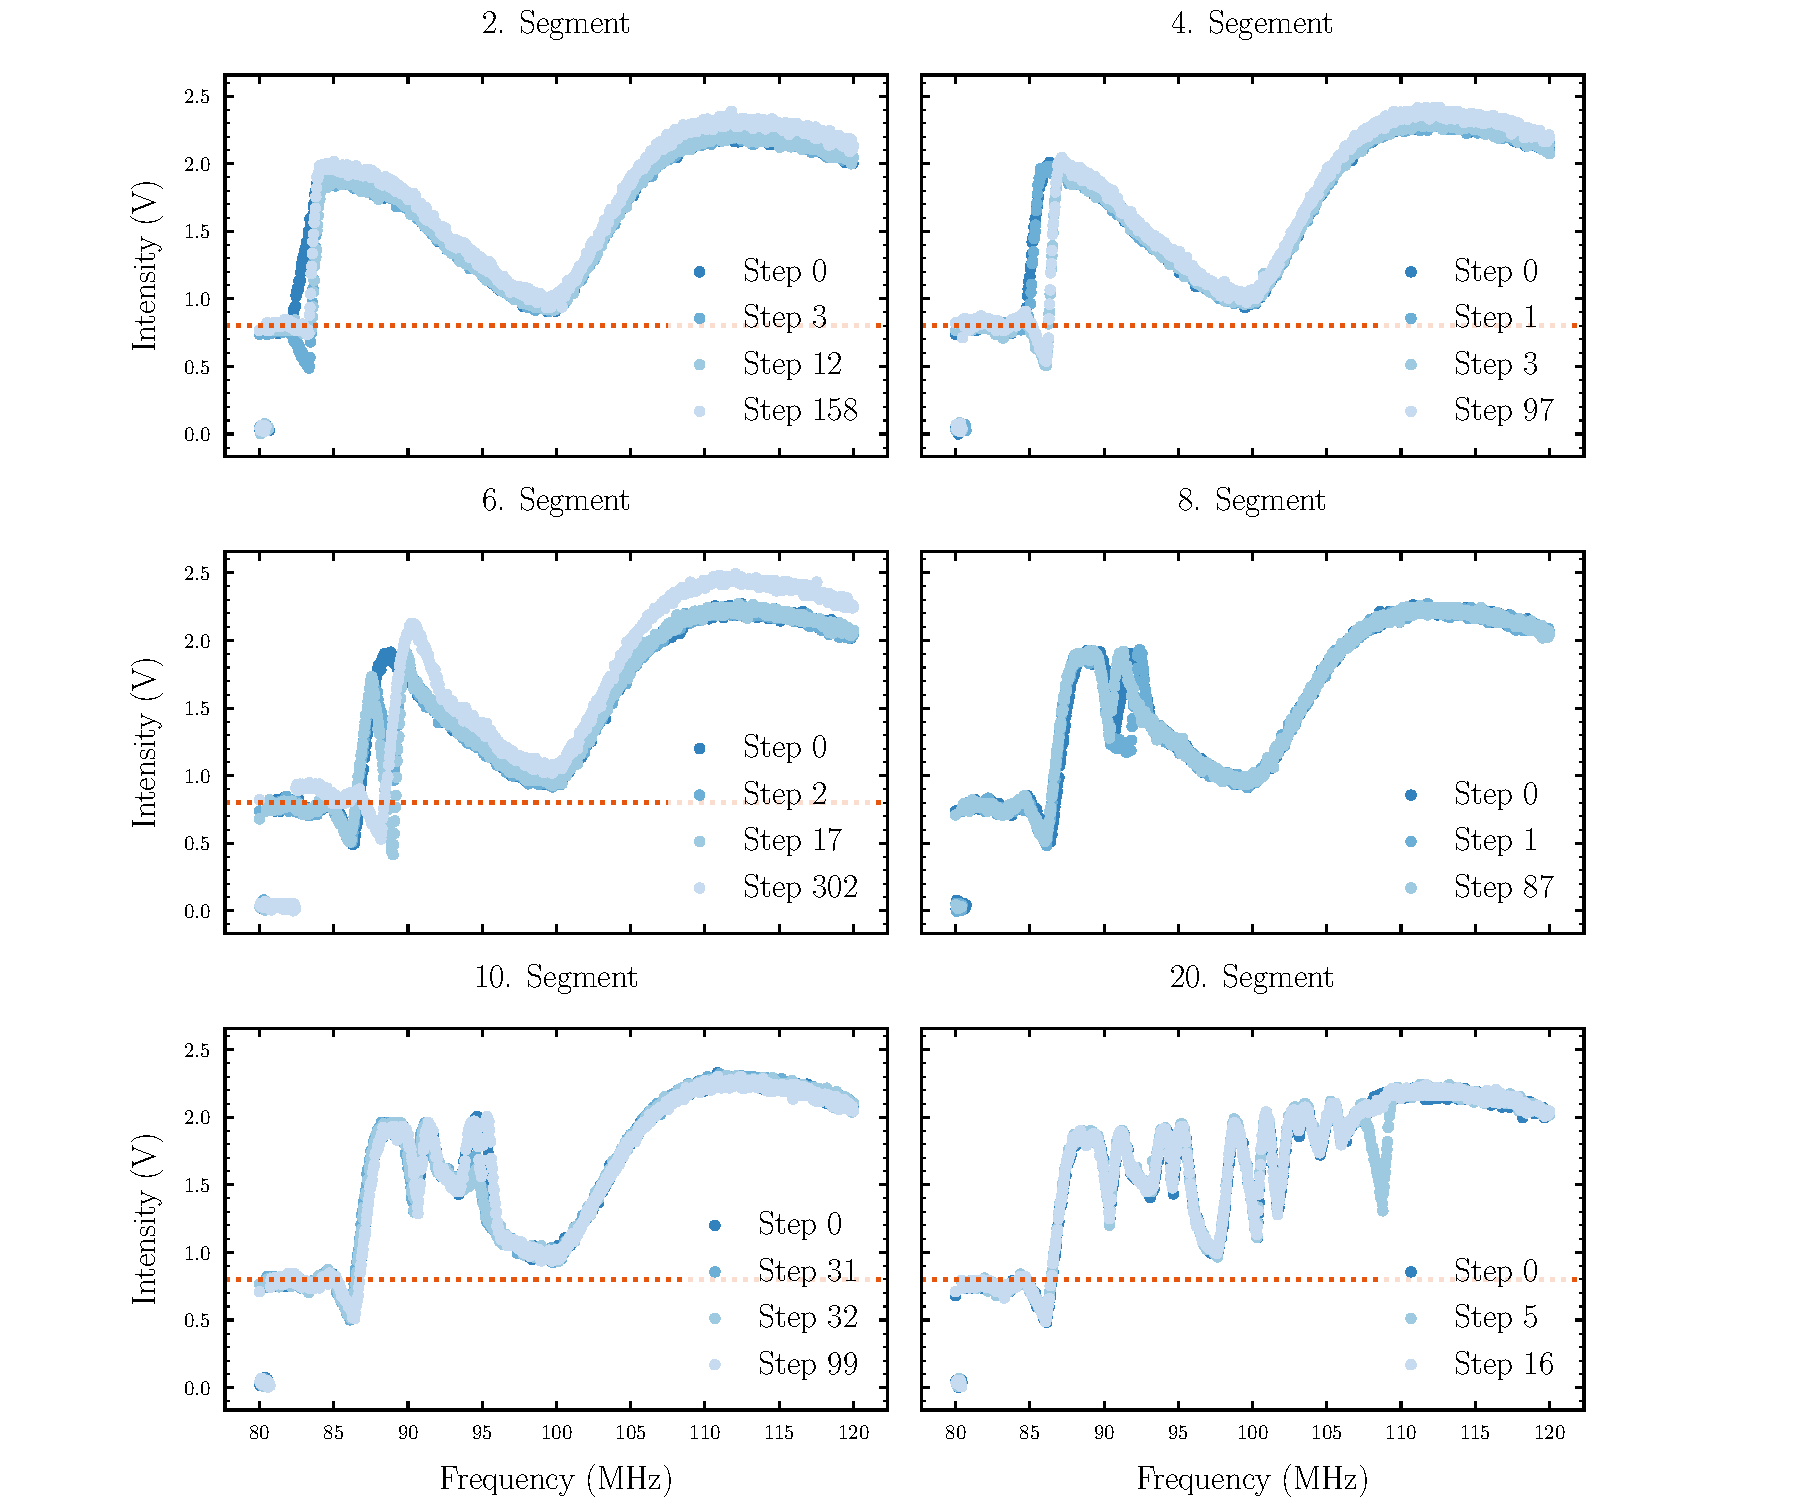
\includegraphics[width=\textwidth]{\figuredir{intensity/optimization/failure.pdf}}
  \captionsetup{width=.8\textwidth}
  \caption{Optimization progress for the 2.,4.,6.,8.,10. and 20. amplitude
  segment of the failed optimization run with 32 amplitude segments. We can
  see that with increasing amplitude segments the non-linear response
  following the optimized amplitude segment increases.}
  \label{fig:intensity_optimization_failure}
\end{figure}

In \Cref{fig:intensity_optimization_failure} we can see the optimization
progress for selected amplitude segments of the optimization run with 32
segments. We observe that with the non-linear response following the actual
optimized amplitude segment increases more and more.

\subsubsection{Summary}

Our attemps to minimize the intensity variance where of mixed success. One
the one hand side we were able to minimize the intensity deviation down
to \SI{100}{\milli\volt} on the other hand we were not able to train any
model on the intensity response that would allow fast optimization or even
predicition of the expected intensity response given an amplitude
configuration.

However we also found out that irregularities arise with increase in the
number of amplitude segments. We suspect that fast changes of the output
amplitude draws power that may non deterministicyl affect the next clock
cycle inside the \gls{dds}. Given that the one dimensional optimizations
already required multiple hours to run and the non-linear response between
amplitude segments we do not believe that it is not in the capabilites of the
\gls{dds} to compensate for the two dimensional intensity distribution
measured in the previous chapter.

\chapter{Conclusion}

\section{Summary}

\section{Future Outlook}

\section{Further Applications}


\printglossaries
\listoffigures
\listoftables
\listoflistings
\printbibliography

\appendix
\chapter{Electronics}

\section{Trigger Hub}
\label{app:electronics:trigger_hub}

The trigger hub is driven by a \SI{3.3}{\volt} input signal and a
\SI{5}{\volt} voltage source. The input signal is amplified to drive four
\gls{ttl} inputs through use of the \gls{sn74128} \cite{SN74128} line driver.
Furthermore the hub is designed to be mounted on the \gls{bbb} which itself
provides the trigger network interface.

\begin{figure}[h]
  \centering
  \captionsetup{width=.8\textwidth}
  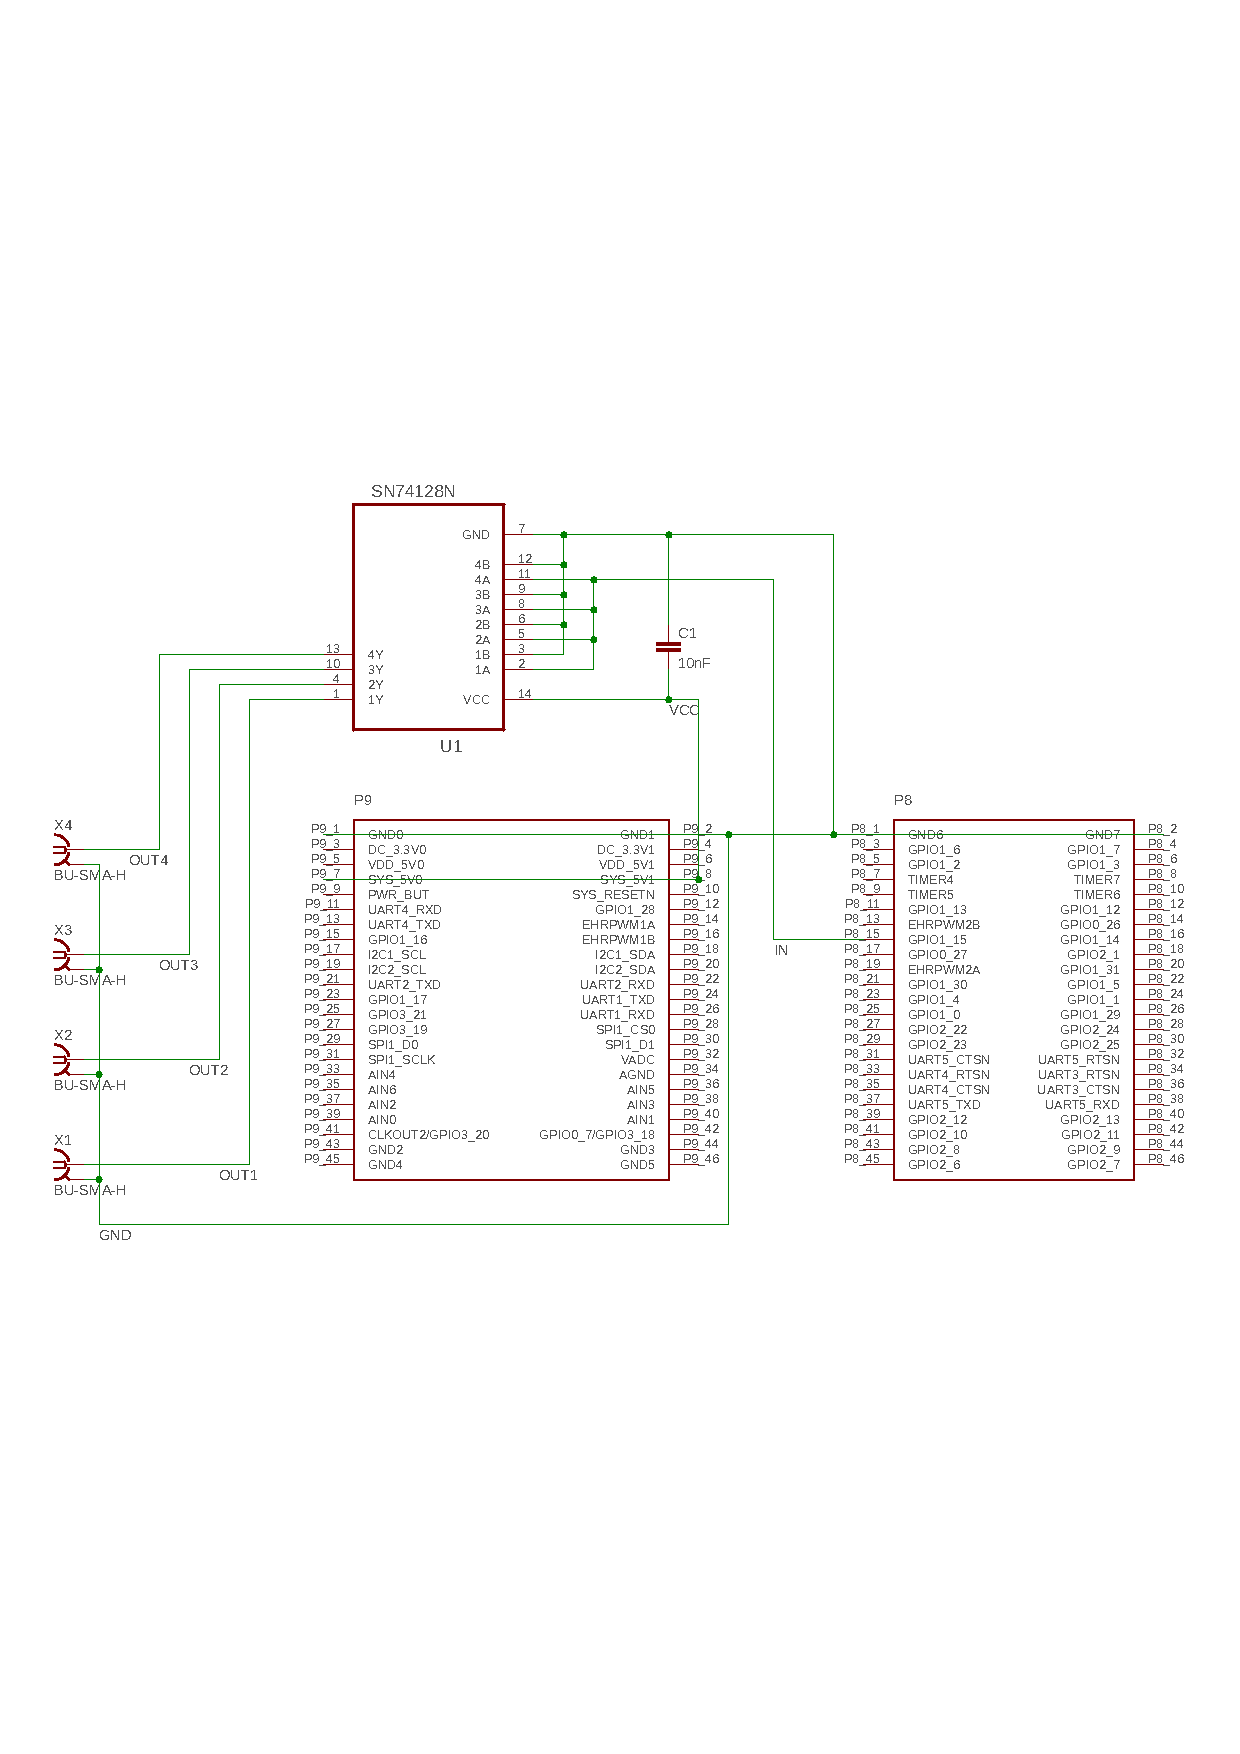
\includegraphics[width=\textwidth]{images/circuits/line-driver/schematic.pdf}
  \caption{Elecronic circuit schematics of the trigger hub. The
    \SI{3.3}{\volt} input signal is amplified by the \gls{sn74128} line
    driver and outputed to four \gls{sma} connectors.}
\end{figure}

The \gls{sn74128} exposes four independent outputs $Y$, each is driven by a
two-input ($A$ and $B$) with NOR ($\overline{A+B}=Y$) logic. As our objective
is to forward rising edge trigger signals we pulled all four $B$ to low by
connecting them with \gls{gnd}. The four $A$ where connected together with
the input signal. The input signal has to transition from $1$ to $0$ in order
to signal a rising edge trigger signal.

\begin{listing}[h]
  \inputminted[xleftmargin=.2\linewidth]{javascript}{scripts/trigger.js}
  \captionsetup{width=.6\linewidth}
  \caption{\gls{bbb} script that starts a \gls{http} server to listen for
requests on which to trigger a rising edge signal. On execution it pulls the
signal \gls{gpio} to high. The request callback then pulls the \gls{gpio} to
low for one \SI{1}{\milli\second}.}
\end{listing}

Using the \gls{bbb} makes it easy to write scripts that communicate with
other devices over the \gls{lan}. We used the bonescript library to access
the \gls{gpio} interface as it is pre-installed on the \gls{bbb}.

\begin{figure}[h]
  \centering
  \begin{minipage}{.40\textwidth}
    \centering
    \includegraphics[width=\linewidth]{images/circuits/line-driver/layout.pdf}
    \captionsetup{width=\linewidth}
    \caption{Board layout of the trigger hub. The source amplifier is designed
to fit on top of the \gls{bbb} expansion headers.}
  \end{minipage}
  \begin{minipage}{.50\textwidth}
    \centering
    \includegraphics[width=.6\linewidth]{images/circuits/line-driver/board.jpg}
    \captionsetup{width=.8\linewidth}
    \caption{Picture of the trigger hub on the \gls{bbb}. The \gls{bbb} is
connected with the \gls{lan} via cable. The trigger hub forwards the signal
to the oscilloscope, the camera and the two \gls{dds}.}
  \end{minipage}
\end{figure}

\chapter{Calibration}

Alterations of the laboratory environment combined with the exchange of
components from the original setup made it advisable to recalibrate the setup.
In this chapter we want to document the steps necessary for calibration for
successive experiments.

\section{Fiber Coupling}

The visually shielded section of the setup used to reduce the output power
of the laser source is optically paired with the open section for beam
deflection via a \gls{smf} that only permits two orthogonal polarization and
a single gaussian mode. Through tuning the polarisator inside the power
reduction section we can try to match one of the orthogonal polarization
modes supported by the \gls{smf}. Polarization discrepancies induce the
polarization inside the \gls{smf} to oscillate on environmental changes like
temperature or vibration. Henceforth it is key to couple polarization modes
in order to ensure a stable operation.

The following receipt has proven to be successful to find an approximate
polarization match between the laser beam and the \gls{smf}. In addition
to the setup described in \cref{sec:powerbox} and \cref{sec:deflection}
an oscilloscope and a hot air gun are highly recommended.

\begin{enumerate}
  \item Connect the photodiode to the oscilloscope and use a coarse time
    scale of i.e. \SI{2}{\second}.
  \item Apply safety measures i.e. put on appropiete laser safety glasses and
    inform present personal of the imminent danger.
  \item Open the cover of the power reduction setup.
  \item Apply heat to the \gls{smf} through the hot air gun, alternatively
    you can try to move the fiber.
  \item The photodiode signal should start to oscillate. Tune the polarizor
    inside the power reduction subject to minimizing the oscillation.
\end{enumerate}

The oscillations occur as the polarization circulates inside the fiber and
will stop at some point. In this case yu should remove the heat or mechanical 
stress on the fiber and wait some time before you can reapply with the initial
response.

\section{Beam Alignment}

As is well known, beams that pass off-centered through spherical lenses
experience optical aberrations. Additionally we found that uncentered beams
may cause further optical defects from reflections at boundaries. Both effects
should be avoided as far as possible by adjusting positions and mirror angles.

As auxilliaries we recommend a pair of iris diaphragms that are mountable to
the lens mounts and a screen i.e. a white sheet of hard paper. With the iris
diaphragms we can easily find a center reference point visually by inspecting
the symmetry of the iris illumination at different pinhole diameters. Exact
steps are summarized in the below receipt. We refer to the optics as annotated
in \cref{fig:deflection}.

\begin{enumerate}
  \item Place screen in front of L2 and adjust screws on fiber coupler subject
    to a clean beam profile on the screen of the (1,1) diffraction order of
    the \gls{aom}s.
  \item Apply one iris to L2 and find center frequency of the \gls{aom}s.
  \item Mount irises on L3 and L4. Mount mirror pair M1, M2 to direct beam
    through both pinholes.
  \item Place auxilliary lens with mounted iris between L7 and M3 and adjust
    second objective pair L6, L7.
  \item Mount iris on L8 and place auxilliary lens with mounted iris in front
    of BS3. Align the mirror pair M3 and M4 to reflect the beam through both
    irises.
  \item Adjust the objective pair distance until you see an output similar to
    XY on the \gls{ccd} camera.
\end{enumerate}

The alignment of a mirror pair can be simplified by using the below algorithm:

\begin{enumerate}
  \item Select axis to align.
  \item Align the beam on the outside lens by tuning the inner mirror.
  \item Align the beam on the inner lens by tuning the outside mirror.
  \item Repeat steps 2 and 3 until beam is aligned on both lenses. Proceed
    with other axis.
\end{enumerate}

\section{Camera Focus}

Finally we had to reposition the camera to focus the incoming beam correctly
in order to register the beam profile as would be seen later by the atoms.
To find the precise focus position we followed the procedure described in
\cite{Hertlein2017} that consits of extracting the camera rail with its lens
and focusing it on a far distant object.

\begin{figure}[ht]
  \centering
  \includegraphics[width=\textwidth]{\builddir{focus.pdf}}
  \caption{Camera focused on far distant object. In this case a window from the
  building accross the courtyard.}
\end{figure}

\section{Beam Profile}

% Image from CCD camera with gaussian fit


\addchap{Declearation of Authorship}

\addsec{Statutory Declearation}

I hereby declare that this thesis has been composed solely by myself except
where indicated otherwise by reference or acknowledgment.

The work presented has not been submitted, in whole or in part, in any
previous application for a degree.

\vspace{1em}
\textbf{Munich, \today}


\end{document}
